\documentclass[UKenglish]{uiomasterthesis} %% ... or norsk or nynorsk or USenglish
\usepackage[utf8]{inputenc} %% ... or latin1
\usepackage[T1]{url}\urlstyle{sf}
\usepackage{babel, csquotes, graphicx, textcomp, uiomasterfp, varioref}
\usepackage{amsthm}
\usepackage{pgf}
\usepackage{tikz}
\usepackage{amsmath, amssymb, amsfonts, bm}
\usepackage{acronym}
\usepackage{multirow}
\usepackage{mathtools}
\usepackage{algorithm}
\usepackage{array}
\usepackage{listings}
\usepackage[table]{xcolor}
\usepackage{listofitems}
\usepackage{pgfplots}
\usepackage{algpseudocode}
\usepackage{tikzlings}
\usepackage[backend=biber,style=numeric-comp, sorting=none]{biblatex}
\usepackage[hidelinks, hypertexnames=false]{hyperref}


\usetikzlibrary{arrows.meta} % for arrow size
\usepackage[outline]{contour} % glow around text
\contourlength{1.4pt}

\usetikzlibrary{positioning, matrix, backgrounds}
\usetikzlibrary{3d,decorations.text,shapes.arrows,fit}

\definecolor{codegreen}{rgb}{0,0.6,0}
\definecolor{codegray}{rgb}{0.5,0.5,0.5}
\definecolor{codepurple}{rgb}{0.58,0,0.82}
\definecolor{backcolour}{rgb}{0.95,0.95,0.92}

\lstdefinestyle{pythonstyle}{
    language=Python,
    backgroundcolor=\color{white},
    commentstyle=\color{codegreen},
    keywordstyle=\color{magenta},
    numberstyle=\tiny\color{codegray},
    stringstyle=\color{codepurple},
    basicstyle=\ttfamily\footnotesize,
    breakatwhitespace=false,
    escapeinside=||,
    breaklines=true,
    captionpos=b,
    keepspaces=true,
    frame=single,
    numbersep=5pt,
    showspaces=false,
    showstringspaces=false,
    showtabs=false,
    tabsize=2,
    morekeywords={self},
}

\lstset{
	breaklines=true,
	style=pythonstyle,
}


\let\origthelstnumber\thelstnumber
\makeatletter
\newcommand*\Suppressnumber{%
  \lst@AddToHook{OnNewLine}{%
    \let\thelstnumber\relax%
     \advance\c@lstnumber-\@ne\relax%
    }%
}

\newcommand*\Reactivatenumber[1]{%
  \setcounter{lstnumber}{\numexpr#1-1\relax}
  \lst@AddToHook{OnNewLine}{%
   \let\thelstnumber\origthelstnumber%
   \refstepcounter{lstnumber}
  }%
}


\makeatother


\pgfplotsset{colormap={turbo}{
   rgb=(0.19,0.07,0.23)
   rgb=(0.24,0.22,0.58)
   rgb=(0.27,0.37,0.82)
   rgb=(0.28,0.50,0.97)
   rgb=(0.23,0.64,0.99)
   rgb=(0.14,0.76,0.89)
   rgb=(0.09,0.87,0.76)
   rgb=(0.17,0.94,0.62)
   rgb=(0.36,0.99,0.45)
   rgb=(0.56,1.00,0.29)
   rgb=(0.71,0.97,0.21)
   rgb=(0.84,0.90,0.21)
   rgb=(0.94,0.80,0.23)
   rgb=(0.99,0.69,0.21)
   rgb=(0.99,0.54,0.15)
   rgb=(0.95,0.38,0.08)
   rgb=(0.88,0.26,0.04)
   rgb=(0.78,0.16,0.01)
   rgb=(0.65,0.08,0.00)
   rgb=(0.48,0.02,0.01)
}}

\tikzset{pics/fake box/.style args={% #1=color, #2=x dimension, #3=y dimension, #4=z dimension
#1 with dimensions #2 and #3 and #4 and #5}{
code={
\draw[thin]  (0,0,0) coordinate(-front-bottom-left) to
++ (0,#3,0) coordinate(-front-top-right) --++
(#2,0,0) coordinate(-front-top-right) --++ (0,-#3,0) 
coordinate(-front-bottom-right) -- cycle;
\draw[thin] (0,#3,0)  --++ 
 (0,0,#4) coordinate(-back-top-left) --++ (#2,0,0) 
 coordinate(-back-top-right) --++ (0,0,-#4)  -- cycle;
\draw[thin] (#2,0,0) --++ (0,0,#4) coordinate(-back-bottom-right)
--++ (0,#3,0) --++ (0,0,-#4) -- cycle;
\path[decorate,decoration={text effects along path, text={#5}}] (#2/2,{2+(#3-2)/2},0) -- (#2/2,0,0);
}
}}
% from https://tex.stackexchange.com/a/52856/121799
\tikzset{circle dotted/.style={dash pattern=on .05mm off 2mm,
                                         line cap=round}}

\pgfdeclarelayer{foreground}
\pgfsetlayers{background, main, foreground}

\renewcommand{\algorithmicrequire}{\textbf{Input:}}
\renewcommand{\algorithmicensure}{\textbf{Output:}}
\newcommand{\R}{\mathbb{R}}

\providecommand{\mathdefault}[1]{#1}


\definecolor{id}{rgb}{0.4, 0.7607843137254902, 0.6470588235294118}
\definecolor{near}{rgb}{0.5529411764705883, 0.6274509803921569, 0.796078431372549}
\definecolor{far}{rgb}{0.9882352941176471, 0.5529411764705883, 0.3843137254901961}

\definecolor{ca0a0a0}{RGB}{160,160,160}
\definecolor{ce0e0e0}{RGB}{224,224,224}
\colorlet{myred}{red!80!black}
\colorlet{myblue}{blue!80!black}
\colorlet{mygreen}{green!60!black}
\colorlet{myorange}{orange!70!red!60!black}
\colorlet{mydarkred}{red!30!black}
\colorlet{mydarkblue}{blue!40!black}
\colorlet{mydarkgreen}{green!30!black}

% STYLES
\tikzset{
  >=latex, % for default LaTeX arrow head
  node/.style={thick,circle,draw=myblue,minimum size=22,inner sep=0.5,outer sep=0.6},
  node in/.style={node,green!20!black,draw=mygreen!30!black,fill=mygreen!25},
  node hidden/.style={node,blue!20!black,draw=myblue!30!black,fill=myblue!20},
  node convol/.style={node,orange!20!black,draw=myorange!30!black,fill=myorange!20},
  node out/.style={node,red!20!black,draw=myred!30!black,fill=myred!20},
  connect/.style={thick,mydarkblue}, %,line cap=round
  connect arrow/.style={-{Latex[length=4,width=3.5]},thick,mydarkblue,shorten <=0.5,shorten >=1},
  node 1/.style={node in}, % node styles, numbered for easy mapping with \nstyle
  node 2/.style={node hidden},
  node 3/.style={node out}
}
\def\nstyle{int(\lay<\Nnodlen?min(2,\lay):3)} % map layer number onto 1, 2, or 3

\title{Explainable Artificial Intelligence for Out-of-Distribution Detection}
\subtitle{Using irregularities in machine learning explanations to detect when a model is faced with unusual data}
\author{Jonatan Hoffmann Hanssen}

\addbibresource{bibliography.bib}

\theoremstyle{definition}
\newtheorem*{definition}{Definition}

\begin{document}


\uiomasterfp[dept={Department of Informatics},
program={Robotics and Intelligent Systems},
supervisors={Hugo Lewi Hammer \and Kyrre Harald Glette}, image={/home/jona/.config/zsh/cat.jpg},
long]

\frontmatter{}
\begin{abstract}
As Artificial Intelligence becomes a larger and larger part of society, the need for robust and understandable models becomes paramount. When neural networks are used in high-impact settings such as cancer detection or autonomous driving, we must require that they 
\end{abstract}

\begin{xabstract}[Sammendrag]
Here comes the abstract in a different language.
\end{xabstract}


\tableofcontents{}
\listoffigures{}
\listoftables{}

\begin{acronym}[ICANN]
    \acro  {ood}   [OOD]   {Out-of-Distribution}
    \acro  {dl}   [DL]   {Deep Learning}
    \acro  {id} [ID] {In-Distribution}
    \acro  {cam} [CAM] {Class Activation Mapping}
    \acro  {gradcam} [GradCAM] {Gradient Class Activation Mapping}
    \acro  {gap}   [GAP]   {Global Average Pooling}
    \acro  {msp}   [MSP]   {Maximum Softmax Probability}
    \acro  {lime}   [LIME]   {Local Interpretable Model-Agnostic Explanations}
    \acro  {relu}   [ReLU]   {Rectified Linear Unit}
    \acro  {mls}   [MLS]   {Maximum Logit Score}
    \acro  {msp}   [MSP]   {Maximum Softmax Probability}
    \acro  {rmd}   [RMD]   {Relative Mean Absolute Difference}
    \acro  {qcd}   [QCD]   {Quartile Coefficient of Determination}
    \acro  {vim}   [VIM]   {Virtual Logit Matching}
    \acro  {sota}   [SoTA]   {State-of-the-Art}

    \acro  {cnn}   [CNN]   {Convolutional Neural Network}
    \acro  {pca}   [PCA]   {Principal Component Analysis}

    \acro  {slic} [SLIC] {Simple Linear Iterative Clustering}

    \acro  {ffnn}[FFNN]{Feed Forward Neural Network}
    \acro  {cv}[CV]{Coefficient of Variance}

    \acro  {gbp}   [GBP]   {Guided Backpropagation}
    \acro  {ml}   [ML]   {Machine Learning}
    \acro  {lrp}   [LRP]   {Layer Relevance Propagation}
    \acro  {xai}   [XAI]   {Explainable Artificial Intelligence}
    \acro  {ai}   [AI]   {Artificial Intelligence}
    \acro  {auroc}   [AUROC]   {Area Under Receiver Operating Characteristic}
    \acro  {aupr}   [AUPR]   {Area Under Precision Recall Curve}
    \acro  {roc}   [ROC]   {Receiver Operating Characteristic}
    \acro  {fpr}   [FPR]   {False Positive Rate}
    \acro  {tpr}   [TPR]   {True Positive Rate}
    \acro  {fpr95}   [FPR95]   {False Positive Rate at 95\% Recall}
\end{acronym}

\begin{preface}
Generative \ac{ai} has \textbf{not} been used to generate or enhance any written text contained in this thesis. However, generative \ac{ai} has been used for some programmatic tasks. Services such as GPT UiO have been used for code debugging, for generating TikZ code used for creating diagrams, and for generating some boilerplate Python code. All data and personal information have been processed in accordance with the University of Oslo's regulations, and I, as the author of the document, take full responsibility for the validity of any generated code used as part of this work.
\end{preface}

\mainmatter{}



\chapter{Introduction}

\section{Motivation}

\ac{ml} generally, and \ac{dl} specifically, have seen a tremendous increase in performance in recent years, performing comparable to humans in tasks such as image classification, speech and handwriting recognition, as well as many others \cite{performance}. Consequently, \ac{dl} methods have been deployed in a multitude of fields and have become a part of our daily lives through their role in web search, text translation, computer vision, and in many other technologies which are taken for granted. In the medical field, deep learning has the potential to provide faster and more accurate detection of diseases by being trained on cases from thousands of previous patients \cite{xaisurvey}. Despite this, the adoption \ac{dl} in high impact fields, such as medicine, has been slow, with \cite{dlmed} stating that: "surprisingly little in health care is driven by machine learning".

% TODO: make these citations more specific

To explain this discrepancy, we should consider that, despite their impressive performance, the application of deep learning methods is not without drawbacks. Firstly, deep neural networks are inherently unexplainable due to the large number of parameters that any non-trivial network has. \ac{sota} models will perform millions of operations to evaluate a single data point, and it is therefore impossible for humans to comprehend and explain the entire process which lead the model to make a particular decision. In medicine, this is a major limitation of deep learning methods, as both doctors and patients expect to be able to understand why a decision was made \cite{tingsim}. In other high-impact fields, such as autonomous driving, this lack of transparency also has serious practical and legal ramifications. % TODO cite this

Secondly, although neural networks may attain high accuracy on test data and appear to have learned great insights about the tasks they are employed in, they often lack robustness and can suffer large drops in performance on data points which are slightly different from the training data. As \cite{intriguing} has shown, it is possible to create data points which are imperceptibly different from normal data points, yet still fool otherwise high performing models. More problematically, unlike humans, who recognize when they are faced with a novel situation where their expertise might be lacking, \ac{dl} methods will predict equally confidently on data points which are far outside the data they have been trained on \cite{tingsim}.

These two problems lead to the fields of \ac{xai}, and \ac{ood} detection. \ac{xai} attempts to explain the reasons why a model came to a decision, which helps to remedy the black-box nature of complicated \ac{dl} models. In a healthcare setting, such explanations can be inspected by medical practitioners to confirm the diagnosis, and can be used to give patients information about why decisions regarding their health were made. In autonomous driving or other automated high impact fields, \ac{xai} can be used to detect failure modes or to understand and improve trained models. \ac{ood} detection attempts to uncover when a data point is too different from the training data to be classified reliably. These methods could alert medical practitioners when such data points occur, thus avoiding potentially fatal misclassifications. In autonomous driving, the system could detect novel situations and cede control back to the user, avoiding accidents.

Both of these fields have seen increased interest in recent years, and are vital parts of any integration of \ac{dl} in high impact settings. As two vibrant fields of study, there is great potential to combining insights from one field to improve performance in the other, an area which is underexplored. This thesis will focus on \ac{ood} detection, but will attempt to use \ac{xai} methods to improve detection performance. The overarching intuition is that by inspecting the explanation of a model on a specific data point, we may be able to uncover flaws or irregularities in the explanation which could help us determine whether the data point is \ac{ood}. This methodology is essentially non-existent in the literature: OpenOOD, the standard \ac{ood} detection benchmarking framework which includes over 40 different methods, contains no methods which use \ac{xai} as part of their functioning.

\section{Problem Statement} \label{section:problemstatement}

As explained in the previous segment, \ac{ood} detection is a developing field, which has become more important in recent years as machine learning is being used for higher impact tasks, such as disease detection, autonomous driving or infrastructure inspection. As reported by \ac{openood15}, there are to date no \ac{ood} detection methods which outperform all others on different benchmarks, which means that there is great potential for further research. Finding novel methods which improve a model's ability to detect when input is \ac{ood} is important to increase the robustness of machine learning models as they are used in these real-world scenarios. The field of \ac{xai} is concerned with understanding the inner workings of a model, and could thus offer insights which can help us detect unusual behaviour in the model as a result of \ac{ood} data points. The problem statement is thus as follows:

\textbf{To what degree can methods from the field of Explainable Artificial Intelligence be used to improve Out-of-Distribution Detection?}
\\

To answer this question, I introduce 3 objectives:

\begin{enumerate}
    \item Develop one or more \ac{ood} detection frameworks which utilize \ac{xai} as part of their functionality, either by combining traditional \ac{ood} detection methods and \ac{xai} explanations, or by using \ac{xai} explanations on their own.
    \item Analyse the behaviour of different \ac{xai} methods on \ac{id} and \ac{ood} data, to be able to develop effective \ac{ood} detectors under the benchmarks created as part of objective 1.
    \item Perform comprehensive tests on the developed \ac{ood} detectors on \ac{sota} \ac{ood} detection benchmarks, to be able to accurately assess the performance of \ac{xai} based \ac{ood} detection in comparison with existing \ac{ood} detection methods.
\end{enumerate}

\section{Scope} \label{section:scope}

As we will see in chapter \ref{chapter:background}, both the fields of \ac{xai} and \ac{ood} detection are very large, which makes it impossible to explore all the possible ways one might combine \ac{xai} and \ac{ood} detection. Thus, it is necessary to restrict the scope of both the \ac{xai} and \ac{ood} detection methods used. In this section, I will describe the choices I've made and give a short explanation. In later chapters, the choices will be justified more thoroughly.

The field of \ac{ood} detection is primarily concerned with image classification tasks. Thus, my project will also deal exclusively with image classification datasets. Given this type of data, the choice of \ac{xai} algorithms naturally gravitates towards post-hoc, saliency based methods. The choice of \ac{ood} detection methods is not significantly restricted by the choice to deal exclusively with image data, but I will exclude methods which use outlier exposure to improve performance, or which require retraining of the model. These choices are informed by \cite{openood}, which have found that outlier data is not necessary to achieve \ac{sota} performance, and that "post-hoc methods [...] are generally no worse than methods that require training". Excluding methods which require training drastically decreases the time required for development and testing of new methods, and is thus suitable for an exploratory thesis such as this one. For image classifiers, I limit myself to \ac{cnn} based models, as they are compatible with a far larger amount of \ac{xai} methods than other computer vision models, such as vision transformers.

\section{Research Methods}

Use ACM.

\section{Ethical Considerations}

What are the ethical considerations?

Computing power, environmental impact

Using ImageNet, CIFAR

Ethics of using ai for high impact tasks

\section{Main Contributions}

In this thesis, the goal has been to investigate whether \ac{xai} methods can be used for \ac{ood} detection, and to introduce proof-of-concept \ac{ood} detection frameworks which use \ac{xai} explanations as part of their functioning. As part of this work, I have developed three frameworks for \ac{xai} based \ac{ood} detection methods, which use the saliency maps (heatmaps) generated by \ac{xai} methods applied to images: {\it Saliency Aggregation}, {\it Saliency Aggregation+Logits} and {\it Saliency\acs*{vim}}. These three frameworks have been thoroughly tested on all four \ac{ood} detection benchmarks included in OpenOOD \cite{openood, openood15}, the de-facto standard \ac{ood} detection benchmarking tool.

Through the testing of these three methods, I show that \ac{xai} methods can indeed be used for \ac{ood} detection, contrary to the results found by previous research \cite{martinez}. The key takeaways of this thesis are as follows:

\begin{itemize}
    \item \ac{xai} saliency mapping methods generate values which can be used to predict \ac{ood} samples comparable to baseline methods. However, most \ac{xai} methods output normalized saliencies, which removes valuable information necessary to perform \ac{ood} detection. By removing this normalization and using raw saliency values, I show substantial improvements over previous methods \cite{martinez}.
    \item A simple aggregation of raw saliency values performs slightly below the baseline methods of \ac{mls} and \ac{msp} on Near-\ac{ood} datasets, and sometimes outperforms the baselines on Far-\ac{ood} datasets. This shows that \ac{xai} saliency maps, on their own, capture enough information about a network's response to a data sample to effectively discriminate between \ac{id} and \ac{ood} data points.% Aggregations which are effective in this regard consider the magnitude of the saliencies, such as the mean or vector norm. Aggregations which capture the statistical dispersion of the saliencies do not differ very much between \ac{id} and \ac{ood} data points.
    \item Depending on the choice of \ac{xai} method, \ac{xai} saliency maps output values which are relatively uncorrelated with traditional baseline \ac{ood} methods. This means that their outputs can be combined with other \ac{ood} detection methods to increase \ac{ood} detection performance. Inspired by the work of \cite{combood}, I combine \ac{xai} saliency aggregates with \ac{mls} by a simple addition. Under this framework, I find that the performance is increased by several percentage points over the baselines in several cases, and in one case performs quite close to the \ac{sota} amongst \ac{ood} detection models which do not retrain the underlying classifier.
    \item Saliency values can also be appended directly to the model logits in \ac{ood} detection methods such as \ac{vim} \cite{vim}, leading to statistically significant improvements over using the method without \ac{xai} saliency values in some cases. However, the improvement in this case is not a strong as when using saliency aggregation.
\end{itemize}

These three frameworks are highly general and enable further research into the integration of \ac{xai} and \ac{ood} detection. In addition, I have had code merged into the codebase for OpenOOD, the definitive \ac{ood} detection framework and benchmarking tool. By improving the code used when benchmarking new \ac{ood} detection methods, I have contributed to the broader field of \ac{ood} detection.

\section{Thesis Outline}

Chapter \ref{chapter:background} gives a short introduction to machine learning, followed by a deeper look at the fields of \ac{xai} and \ac{ood} detection. Chapter \ref{chapter:methodology} introduces my methodology; the methods I have used to compare and contrast \ac{xai} explanations on \ac{id} and \ac{ood} data, as well as the three general \ac{ood} detection frameworks which integrate explanations into their functioning. Furthermore, I introduce the different benchmarks which have been used to test each method, the statistical methods used to ensure that the results are statistically significant and the software and hardware architecture used. \ref{chapter:experiments} first goes into the results of the comparison between \ac{id} and \ac{ood} explanations, detailing the differences between different \ac{xai} methods. These investigations have been done on validation benchmarks which are not used during testing, to ensure unbiased results. Based on these results, I have chosen a selection of \ac{xai} \ac{ood} detection methods under these frameworks. These frameworks are then tested on bootstrapped testing benchmarks and compared against baseline methods using statistical analysis. After the experiments follow a discussion (chapter \ref{chapter:discussion}), where I reflect on the benefits and drawbacks of using \ac{xai} methods for \ac{ood} detection, and summarize the results from \ref{chapter:experiments}. Furthermore, the discussion also uses the results from chapter \ref{chapter:experiments} to answer the research question stated in the preceding section. Finally, the conclusion (chapter \ref{chapter:conclusion}) gives a short conclusion of my findings, and envisions a way forward for future work.

\chapter{Background} \label{chapter:background}

In this chapter, I give a short introduction to important concepts in the field of machine learning generally, followed by a more in-depth look at the fields of \ac{ood} detection and \ac{xai}. Finally, I give an overview of related works; papers which have attempted to use \ac{xai} for \ac{ood} detection.

\section{Machine Learning}

Machine Learning is the field of algorithms that are able to learn from data, as opposed to being explicitly programmed. Such algorithms use statistical methods to learn relationships in data, and use these relationships to generalize to unseen data. More formally, \cite{mitchell} gives the following definition of machine learning algorithms:

\begin{definition}
A computer program is said to learn from experience $E$ with respect to some class of tasks $T$ and performance measure $P$ if its performance at tasks in $T$, as measured by $P$, improves with experience $E$.
\end{definition}

Thus, machine learning is a different paradigm from traditional problem solving, where programs are made to solve problems by following explicit rules. For example, a traditional image classification system attempting to differentiate between malignant and benign tumors might use hand-crafted rules which consider the texture, color and size of a tumor, developed by medical professional with years of experience. As one might imagine, such rules will quickly become very complicated when we consider all the possible factors which might influence the appearance of a tumor. Using a machine learning approach, we would instead feed an algorithm with thousands of images of both benign and malignant tumors, and the rules could then be automatically updated until the algorithm predicted the correct category with a high enough accuracy.

Machine Learning is commonly divided into the three subcategories of supervised, unsupervised and reinforcement learning

% A simple comparison is between the two chess engines Stockfish and AlphaZero. Stockfish plays chess by evaluating possible moves according to metrics created by humans\footnote{This is actually no longer the case, as the classical evaluation has been replaced by a neural network (a machine learning approach), however, I will pretend that it still is for the sake of argument}, such as valuing a Queen as equivalent to nine pawns and a 

\subsection{Supervised Learning}

Supervised Learning is a subcategory of machine learning where we have a dataset containing both inputs and desired outputs. In the example above, we could use supervised learning by creating a dataset of images of tumors (the input) and corresponding labels which indicate whether each tumor is malignant or benign (the desired output). The learning goal of the algorithm is then to associate images with the correct label. Because we know the correct answer, we are able to fine-tune the algorithm automatically whenever it makes a mistake. However, supervised learning requires labeled data, which can be very costly, especially in the medical domain, where deciding whether a tumor is malignant or benign requires expert knowledge.

\subsection{Unsupervised Learning}

In unsupervised learning, we do not have any labels. In these cases, we might not know whether data points belong to different classes or not. Instead, we can use machine learning to uncover patterns in the data, for example by attempting to cluster the data into different groups and seeing if these groups are sufficiently separated. An example use case could be for fraud detection in a bank. By feeding financial transaction from many different users into an unsupervised learning model and asking it to perform clustering of the data, it might be possible to find a group of users whose transactions differ substantially from the rest, which might indicate that their transactions are fraudulent.

\subsection{Reinforcement Learning}

Reinforcement Learning deals with problems where we do not know exactly what the correct solution is, but we are able to assess whether a given solution is good or not. For example, when controlling a robot arm, it is difficult to say exactly what angles each joint should be for every millisecond when picking up an object, but if the arm does not pick up the object, we know the algorithm has failed. In these problems, the algorithm is trained through reinforcement, where good attempts are rewarded and bad attempts are punished.

\section{Neural Networks}

Neural Networks constitute a class of machine learning algorithms which have become the clear \ac{sota} in almost all fields where machine learning is applied. Notable examples are computer vision, image classification, speech recognition, text and image generation and machine translation. Neural networks are loosely inspired by our own brains, where neurons are connected together and send information between each other. By connecting thousands of neurons together, neural networks are able to learn complicated relationships between the input and output.

\subsection{Feed Forward Neural Networks}

The \ac{ffnn}, also known as a Multilayer Perceptron, traces its roots to the very beginning of machine learning, through the work of Frank Rosenblatt \cite{rosenblatt}. It forms the basic structure for neural networks which has been adapted and modified over the years to form more complex architectures such as convolutional, recurrent or residual neural networks. The basic structure of an \ac{ffnn} is that the input values are passed through an affine transformation (a matrix multiplication followed by the addition of a bias), and then passed through an activation function, which produces outputs. These outputs can then go through the same process again, which constitutes a single "layer". By stacking several of these layers, with non-linear activation functions, an \ac{ffnn} is able to learn arbitrarily complex mappings between inputs and outputs\footnote{In fact, by the Universal Approximation Theorem \cite{uat}, only a single hidden layer between the input and output is necessary, although this theorem does not give a way to construct such a network for any given function}. Figure \ref{fig:ffnn}\footnote{Figure by Izaak Neutelings, "Neural Network with coefficients, arrows", TikZ.net, licensed under CC BY-SA 4.0, [\url{https://tikz.net/neural\_networks/}].} shows a simple \ac{ffnn} architecture with three hidden layers. In this case, the bias has been omitted for brevity. Here, we can see how all nodes of a layer are connected to the following layer. By using an activation function on the nodes of the hidden layer, before their values are sent to the next layer, we achieve the non-linearity required to learn complex patterns.

\begin{figure}[H]
    \begin{center}

    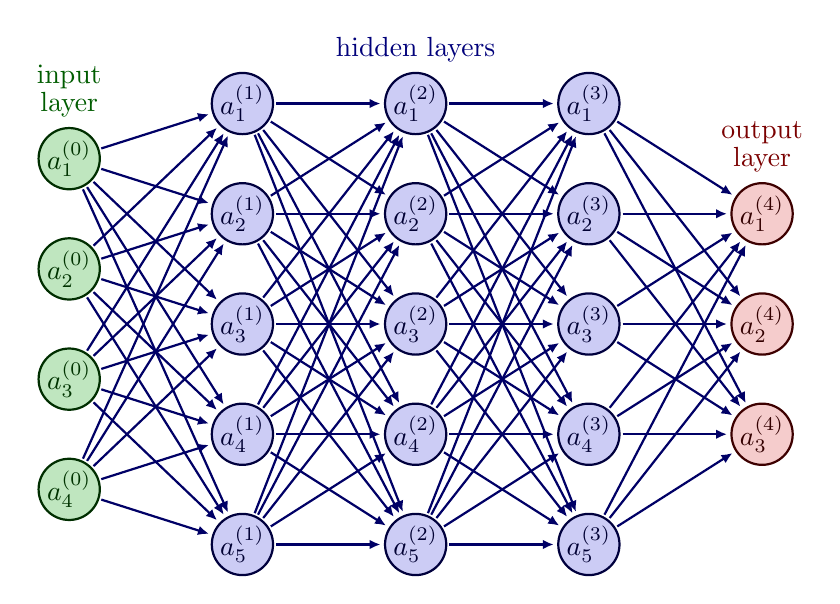
\begin{tikzpicture}[x=2.2cm,y=1.4cm]
  \message{^^JNeural network with arrows}
  \readlist\Nnod{4,5,5,5,3} % array of number of nodes per layer
  
  \message{^^J  Layer}
  \foreachitem \N \in \Nnod{ % loop over layers
    \edef\lay{\Ncnt} % alias of index of current layer
    \message{\lay,}
    \pgfmathsetmacro\prev{int(\Ncnt-1)} % number of previous layer
    \foreach \i [evaluate={\y=\N/2-\i; \x=\lay; \n=\nstyle;}] in {1,...,\N}{ % loop over nodes
      
      % NODES
      \node[node \n] (N\lay-\i) at (\x,\y) {$a_\i^{(\prev)}$};
      %\node[circle,inner sep=2] (N\lay-\i') at (\x-0.15,\y) {}; % shifted node
      %\draw[node] (N\lay-\i) circle (\R);
      
      % CONNECTIONS
      \ifnum\lay>1 % connect to previous layer
        \foreach \j in {1,...,\Nnod[\prev]}{ % loop over nodes in previous layer
          \draw[connect arrow] (N\prev-\j) -- (N\lay-\i); % connect arrows directly
          %\draw[connect arrow] (N\prev-\j) -- (N\lay-\i'); % connect arrows to shifted node
        }
      \fi % else: nothing to connect first layer
      
    }
    
  }
  
  % LABELS
  \node[above=0,align=center,mygreen!60!black] at (N1-1.90) {input\\[-0.2em]layer};
  \node[above=0,align=center,myblue!60!black] at (N3-1.90) {hidden layers};
  \node[above=0,align=center,myred!60!black] at (N\Nnodlen-1.90) {output\\[-0.2em]layer};
  

    \end{tikzpicture}
    \end{center}
    \caption[Feed Forward Neural Network]{Figure showing a simple Feed Forward Neural Network, with nodes labeled. The number in parentheses indicates the layer number while the subscript indicates the node number within the layer.}
    \label{fig:ffnn}
\end{figure}



Mathematically, a single layer can then be described as follows:

\begin{equation}
\bm{x_{i+1}} = \sigma_i (A_i \bm{x_i} + \bm{b_i})
\label{ffnn}
\end{equation}

Here, the input $\bm{x_i}$ is linearly transformed by the weights of the matrix $A_i$ from the input space to the output space, then each value of the new vector in the output space is adjusted by an addition of a bias term, and finally an activation function ($\sigma_i$) is applied to each value. The size of the input and output layers is determined by the number of input and output features, respectively. Furthermore, the activation function of the output layer is also determined by the application, most commonly {\it sigmoid} for binary classification, {\it softmax} for multi-class classification and simply identity for regression.


\subsection{Convolutional Neural Networks} \label{section:cnn}

\acp{ffnn} have some inherent flaws which make them unsuitable for working with high dimensional, spatially connected data, such as the pixels which make up an image. Firstly, each input of a \ac{ffnn} is connected to every output of the following layer. If we want to connect the input pixels of a $224$ by $224$ image to a layer of 100 nodes, our first layer will have over 5 million weights, which is already quite a lot for a relatively small image. Furthermore, these weights will have to encode redundant information, because each pixel is considered separately. Consider a network attempting to detect the presence of a cat in an image: We would want the network to detect the cat regardless of whether it is in the middle, the right corner, or any other position in the image. In an \ac{ffnn}, the weights connected to any of these positions in the image would then have to encode a cat detector separately from all the others.

\acp{cnn} solve both these issues by using small kernels of weights which are "slid" across the entire input. By using the same weights across all positions of the image, we do not need to train separate detectors for different positions, giving us translation invariance. Figure \ref{fig:conv} shows the functioning of a convolutional kernel on a 3-channel image. Each value in the output is a weighted sum of a neighbourhood of values in the input image, where the weights are defined by the kernel. As we can see, the same weights are used on all positions, drastically reducing the number of parameters that need to be tuned. In a 2d-convolution, the kernel has the same number of channels as the input, and is only slid across the height and width dimension. The kernel in this figure is a {\it Sobel Operator}, and detects vertical edges. In a \ac{cnn}, the weights of each kernel are not specified manually, but rather learned through backpropagation.

\begin{figure}[H]
    \begin{center}

        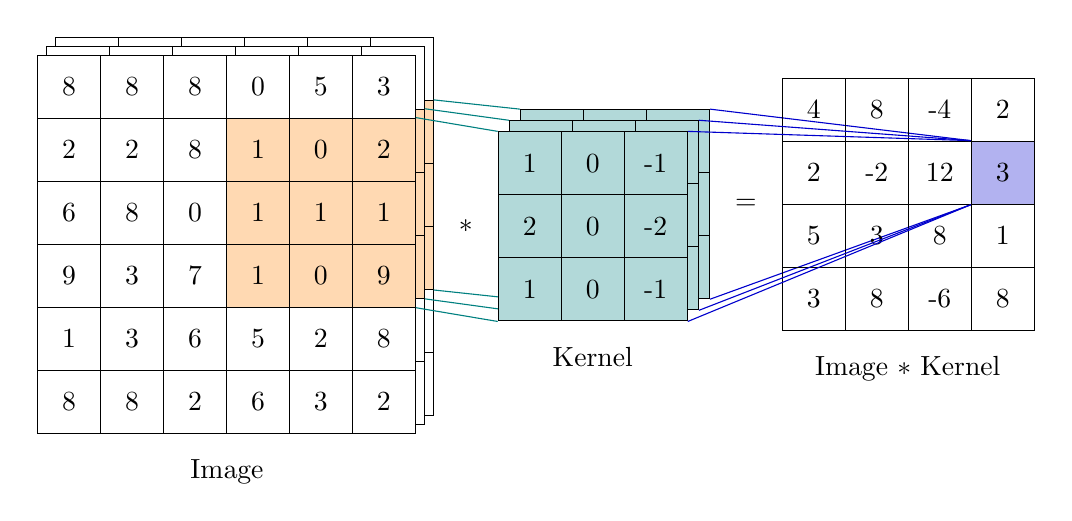
\begin{tikzpicture}[
    2d-arr/.style={minimum size=0.8cm, matrix of nodes, row sep=-\pgflinewidth, column sep=-\pgflinewidth, nodes={draw}}
  ]

  \begin{pgfonlayer}{foreground}
      \matrix (mtr) [2d-arr] {
      |[fill=white]| 8 & |[fill=white]| 8 & |[fill=white]| 8 & |[fill=white]| 0 & |[fill=white]| 5 & |[fill=white]| 3\\
      |[fill=white]| 2 & |[fill=white]| 2 & |[fill=white]| 8 & |[fill=orange!30]| 1 & |[fill=orange!30]| 0 & |[fill=orange!30]| 2\\
      |[fill=white]| 6 & |[fill=white]| 8 & |[fill=white]| 0 & |[fill=orange!30]| 1 & |[fill=orange!30]| 1 & |[fill=orange!30]| 1\\
      |[fill=white]| 9 & |[fill=white]| 3 & |[fill=white]| 7 & |[fill=orange!30]| 1 & |[fill=orange!30]| 0 & |[fill=orange!30]| 9\\
      |[fill=white]| 1 & |[fill=white]| 3 & |[fill=white]| 6 & |[fill=white]| 5 & |[fill=white]| 2 & |[fill=white]| 8\\
      |[fill=white]| 8 & |[fill=white]| 8 & |[fill=white]| 2 & |[fill=white]| 6 & |[fill=white]| 3 & |[fill=white]| 2\\
      };
  \end{pgfonlayer}

  \begin{pgfonlayer}{main}
      \matrix (mtr2) [2d-arr, above right=-7 cm of mtr] {
          |[fill=white]| 1 & |[fill=white]| 1 & |[fill=white]| 1 & |[fill=white]| 0 & |[fill=white]| 0 & |[fill=white]| 0\\
          |[fill=white]| 0 & |[fill=white]| 1 & |[fill=white]| 1 & |[fill=orange!30]| 1 & |[fill=orange!30]| 0 & |[fill=orange!30]| 0\\
          |[fill=white]| 0 & |[fill=white]| 0 & |[fill=white]| 1 & |[fill=orange!30]| 1 & |[fill=orange!30]| 1 & |[fill=orange!30]| 0\\
          |[fill=white]| 0 & |[fill=white]| 0 & |[fill=white]| 1 & |[fill=orange!30]| 1 & |[fill=orange!30]| 0 & |[fill=orange!30]| 0\\
          |[fill=white]| 0 & |[fill=white]| 1 & |[fill=white]| 1 & |[fill=white]| 0 & |[fill=white]| 0 & |[fill=white]| 0\\
          |[fill=white]| 1 & |[fill=white]| 1 & |[fill=white]| 0 & |[fill=white]| 0 & |[fill=white]| 0 & |[fill=white]| 0\\
      };
    \end{pgfonlayer}

  \begin{pgfonlayer}{background}
      \matrix (mtr3) [2d-arr, above right=-7 cm of mtr2] {
          |[fill=white]| 1 & |[fill=white]| 1 & |[fill=white]| 1 & |[fill=white]| 0 & |[fill=white]| 0 & |[fill=white]| 0\\
          |[fill=white]| 0 & |[fill=white]| 1 & |[fill=white]| 1 & |[fill=orange!30]| 1 & |[fill=orange!30]| 0 & |[fill=orange!30]| 0\\
          |[fill=white]| 0 & |[fill=white]| 0 & |[fill=white]| 1 & |[fill=orange!30]| 1 & |[fill=orange!30]| 1 & |[fill=orange!30]| 0\\
          |[fill=white]| 0 & |[fill=white]| 0 & |[fill=white]| 1 & |[fill=orange!30]| 1 & |[fill=orange!30]| 0 & |[fill=orange!30]| 0\\
          |[fill=white]| 0 & |[fill=white]| 1 & |[fill=white]| 1 & |[fill=white]| 0 & |[fill=white]| 0 & |[fill=white]| 0\\
          |[fill=white]| 1 & |[fill=white]| 1 & |[fill=white]| 0 & |[fill=white]| 0 & |[fill=white]| 0 & |[fill=white]| 0\\
      };
    \end{pgfonlayer}

  \node[below=of mtr-5-3.south east] {Image};

  \node[right=0.2em of mtr3] (str) {$*$};

  \begin{pgfonlayer}{foreground}
  \matrix (K) [2d-arr, right=0.2em of str, nodes={draw, fill=teal!30}] {
    1 & 0 & -1 \\
    2 & 0 & -2 \\
    1 & 0 & -1 \\
  };
  \end{pgfonlayer}

  \begin{pgfonlayer}{main}
  \matrix (K2) [2d-arr, below left=-3.965cm of K, nodes={draw, fill=teal!30}] {
    1 & 0 & 1 \\
    0 & 1 & 0 \\
    1 & 0 & 1 \\
  };
  \end{pgfonlayer}

  \begin{pgfonlayer}{background}
  \matrix (K3) [2d-arr, below left=-3.965cm of K2, nodes={draw, fill=teal!30}] {
    1 & 0 & 1 \\
    0 & 1 & 0 \\
    1 & 0 & 1 \\
  };
  \end{pgfonlayer}

  \node[below=of K-2-2] {Kernel};

  \node[right=0.2em of K3] (eq) {$=$};

  \matrix (ret) [2d-arr, right=0.2em of eq] {
  4 & 8 & -4 & 2\\
  2 & -2 & 12 & |[fill=blue!80!black!30]| 3\\
  5 & 3 & 8 & 1\\
  3 & 8 & -6 & 8\\
  };
  \node[below=of ret-3-3.south west] {Image $*$ Kernel};

  \begin{pgfonlayer}{foreground}
      \draw[teal] (mtr-4-6.south east) -- (K-3-1.south west);
      \draw[teal] (mtr-2-6.north east) -- (K-1-1.north west);

      \draw[blue!80!black] (K-1-3.north east) -- (ret-2-4.north west);
      \draw[blue!80!black] (K-3-3.south east) -- (ret-2-4.south west);
  \end{pgfonlayer}

  \begin{pgfonlayer}{main}
      \draw[teal] (mtr2-4-6.south east) -- (K2-3-1.south west);
      \draw[teal] (mtr2-2-6.north east) -- (K2-1-1.north west);

      \draw[blue!80!black] (K2-1-3.north east) -- (ret-2-4.north west);
      \draw[blue!80!black] (K2-3-3.south east) -- (ret-2-4.south west);
  \end{pgfonlayer}

  \begin{pgfonlayer}{background}
      \draw[teal] (mtr3-4-6.south east) -- (K3-3-1.south west);
      \draw[teal] (mtr3-2-6.north east) -- (K3-1-1.north west);

      \draw[blue!80!black] (K3-1-3.north east) -- (ret-2-4.north west);
      \draw[blue!80!black] (K3-3-3.south east) -- (ret-2-4.south west);
  \end{pgfonlayer}


\end{tikzpicture}

    \end{center}
    \caption[Convolution example]{Figure showing a convolutional kernel applied to a 3-channel image.}
    \label{fig:conv}
\end{figure}

By using several different kernels, we can detect many different patterns despite each kernel only detecting a single type. By using the outputs of all the kernels as inputs to a new set of kernels, we can use the same type layer structure as in an \ac{ffnn}, allowing us to extract information in a hierarchical manner. It is common to see that trained \acp{cnn} have early layers that detect edges and texture, later layers that use these edge and pattern detections to detect larger shapes, while the final layers combine the shapes to detect entire objects \cite{lenet5}.

By not evaluating every possible position in the input image, \acp{cnn} downsample the image, and are able to reduce the number of operations considerably. Simultaneously, this downsampling enables each subsequent layer to consider a larger area of the input image than the previous (a larger field-of-view), which allows larger patterns to be discovered. Simultaneously, it is common to use a larger and larger amounts of kernels on the new input, thus increasing the channel depth while the spatial dimensions are reduced. Between each layer, we use non-linear activation functions, similarly to how the are used in \acp{ffnn}.

After several such convolutions, we can flatten the output, either by aggregating each channel using \ac{gap} or a similar method, or we can simply flatten all dimensions and consider the three dimensional feature map as a long vector of shape $C \times H \times W$. By doing this, we can pass the output to one or more linear layers, which can perform classification or regression on the extracted features and give us a final prediction. Figure \ref{fig:cnn2} shows a high level overview of this process. Here, the input, which has only 3 channels, has its spatial dimensions reduced while its channel depth increases through consecutive convolutions. Finally, we have a certain number of channels in our final feature map, which are flattened (in this case with \ac{gap}) and processed through a linear layer to give a final prediction.


\begin{figure}[H]
    \begin{center}
    \end{center}


    \newcommand{\drawRectangles}[5]{
    % #1: Starting x-coordinate
    % #2: Starting y-coordinate (top)
    % #3: Rectangle size
    % #4: Spacing between rectangles
    % #5: Number of rectangles


    % Loop to draw rectangles
    \foreach \i in {0, 1, ..., \the\numexpr#5-1} {
        % Calculate x-coordinate for the current rectangle
        \pgfmathsetmacro{\x}{#1 + \i * #4)}
        \pgfmathsetmacro{\y}{#2 - \i * #4)}
        
        \pgfmathsetmacro{\fillColor}{mod(\i, 2) ? "ce0e0e0" : "ca0a0a0"}
        
        % Draw the rectangle
        \path[draw=black, fill=\fillColor, opacity=1, line width=0.0cm] 
            (\x, \y) rectangle (\x + #3, \y - #3);
    }
}


\def \globalscale {0.7}
\begin{tikzpicture}[y=1cm, x=1cm, yscale=\globalscale,xscale=\globalscale, every node/.append, inner sep=0pt, outer sep=0pt]
  \begin{scope}[shift={(3.5, 0.3)}]
    \path[draw=black,fill=red!20,opacity=1, line width=0.0cm] (12.6, 16.2) 
  rectangle (18.6, 10.3);
    \path[draw=black,fill=green!20,opacity=1, line width=0.0cm] (12.7, 16.1) 
  rectangle (18.7, 10.2);
    \path[draw=black,fill=blue!20,opacity=1, line width=0.0cm] (12.8, 16) 
  rectangle (18.8, 10.1);

    \begin{scope}[shift={(14, 11)}]
        \marmot[scale=1.3, body=blue]
        \bear[xshift=2.4cm, yshift=2.5cm, body=blue]
        \coati[rotatehead=-15, xshift=2.6cm, yshift=-0.5cm, body=blue]
    \end{scope}

    \drawRectangles{19.9}{15.0}{3.0}{0.1}{8}

    \drawRectangles{23.9}{14.8}{1.5}{0.12}{16}

    \drawRectangles{26.9}{15.3}{0.4}{0.133}{32}



    \path[draw=black,fill,fill opacity=0.0,draw opacity=1, line width=0.2mm] 
  (16.4, 14.3) rectangle (16.6, 14.1);
    \path[draw=black,fill,fill opacity=0.0,draw opacity=1, line width=0.2mm] 
  (21.3, 12.4) rectangle (21.7, 12.0);
    \path[draw=black,fill,fill opacity=0.0,draw opacity=1, line width=0.2mm] 
  (26.2, 11.9) rectangle (26.4, 11.7);

    \path[draw=black,fill,draw opacity=1, line width=0.2mm] (16.6, 14.1) -- 
  (22.6, 13.3);
    \path[draw=black,fill,draw opacity=1, line width=0.2mm] (16.6, 14.3) -- 
  (22.6, 13.3);
    \path[draw=black,fill,draw opacity=1, line width=0.2mm] (21.7, 12.0) -- 
  (26.2, 11.8);
    \path[draw=black,fill,draw opacity=1, line width=0.2mm] (21.7, 12.4) -- 
  (26.2, 11.8);
    \path[draw=black,fill,draw opacity=1, line width=0.2mm] (26.4, 11.7) -- 
  (31.1, 11.0);
    \path[draw=black,fill,draw opacity=1, line width=0.2mm] (26.4, 11.9) -- 
  (31.1, 11.0);

    \path[draw=black,fill=ce0e0e0,opacity=1, line width=0.0mm] (30.8, 13.5) -- 
  (31.1, 13.5) -- (32.0, 12.6) -- (31.7, 12.6) -- (30.8, 13.5)-- cycle;;
    \path[draw=black,fill=ce0e0e0,opacity=1, line width=0.0mm] (32.0, 13.2) -- 
  (32.3, 13.2) -- (32.6, 12.9) -- (32.3, 12.9) -- (32.0, 13.2)-- cycle;;

    \path[draw=black,fill,draw opacity=1, line width=0.2mm] (31.41, 11.15) -- 
  (31.7, 12.6);
    \path[draw=black,fill,draw opacity=1, line width=0.2mm] (27.3, 15.3) -- 
  (30.8, 13.5);
    \path[draw=black,fill,draw opacity=1, line width=0.2mm] (32.0, 12.6) -- 
  (32.3, 12.9);
    \path[draw=black,fill,draw opacity=1, line width=0.2mm] (31.1, 13.5) -- 
  (32.0, 13.2);


    \node[anchor=south west] (text10) at (19.9, 10.0){Conv};
    \node[anchor=south west] (text11) at (24.3, 10.0){Conv};
    \node[anchor=south west] (text12) at (27.9, 10.0){Conv};
    \node[anchor=south west] (text13) at (31.9, 11.0){GAP};
    \node[anchor=south west, align=left] (text14) at (12.6, 16.5){Input RGB Image:\\3@224x224};
    \node[anchor=south west] (text15) at (19.9, 15.4){8@112x112};
    \node[anchor=south west] (text16) at (23.9, 15.2){16@56x56};
    \node[anchor=south west] (text17) at (26.9, 15.7){32@14x14};
    \node[anchor=south west] (text18) at (30.8, 13.9){1x32};
    \node[anchor=south west] (text19) at (32.0, 13.6){1x10};
  \end{scope}



\end{tikzpicture}

    \caption[CNN example]{Figure showing a high level overview of how a CNN functions}
    \label{fig:cnn2}
\end{figure}


% \begin{figure}[H]
%     \begin{center}
%
%
%     \begin{tikzpicture}[x={(1,0)},y={(0,1)},z={({cos(60)},{sin(60)})}, scale=1.5]
% %
% % comment these out if you want to see where the axes point to
% % \draw[-latex] (0,0,0) -- (3,0,0) node[below]{$x$};
% % \draw[-latex] (0,0,0) -- (0,3,0) node[left]{$y$};
% % \draw[-latex] (0,0,0) -- (0,0,3) node[below]{$z$};
% % a plane
% \draw pic (box1-1) at (1,-1.6/2,0) {fake box=white!70!gray with dimensions {1/1.6/1.6} and {2*1.6} and {1*1.6} and Input};
%
% \foreach \X [count=\Y] in {1.4,1.2,1.2,1}
% {
%     \draw pic (box1-\Y) at (\Y+1,-\X/2,0) {fake box=white!70!gray with dimensions {1/\X/\X} and {2*\X} and {1*\X} and Conv};
% }
%
% \foreach \X/\Col in {6.5/blue,6.7/red,6.9/lightgray, 7.1/lightgray, 7.3/green}
% {\draw[canvas is yz plane at x = \X, transform shape, fill =
% \Col!50!white] (0,0.10) rectangle (1,-0.5);}
% % \draw[gray!60,thick] (6.3,-0.1,-1.6) coordinate (1-1) -- (6.3,-0.1,0.6) coordinate (1-2) -- (6.3,2.,0.6) coordinate (1-3) -- (6.3,2.1,-1.6) coordinate (1-4) -- cycle;
% % \draw[gray!60,thick] (7.1,-0.1,-1.6) coordinate (2-1) -- (7.1,-0.1,0.6) coordinate (2-2) -- (7.1,2.,0.6) coordinate (2-3) -- (7.1,2.1,-1.6) coordinate (2-4) -- cycle;
% % \foreach \X in {4,1,3}
% % {\draw[gray!60,thick] (1-\X) -- (2-\X);}
% %
% \node[draw,single arrow, fill=blue!10] at (8,0.5,0) {GAP};
% \node[circle,draw,blue,fill=blue!30] (A1) at (9,1,0) {~~~};
% \node[circle,draw,red,fill=red!30,below=4pt of A1] (A2) {~~~};
% \node[circle,draw,green,fill=green!30,below=18pt of A2] (A3) {~~~};
% \draw[circle dotted, line width=2pt,shorten <=3pt] (A2) -- (A3);
% \node[circle,draw,gray,fill=gray!20] (B1) at (10,1,0) {~~~};
% \node[circle,draw,fill=gray!60,below=4pt of B1] (B2) {~~~};
% \node[circle,draw,gray,fill=gray!20,below=18pt of B2] (B3) {~~~};
% \draw[circle dotted, line width=2pt,shorten <=3pt] (B2) -- (B3);
% \begin{scope}[on background layer]
% \node[orange,thick,rounded corners,fill=blue!10,fit=(A1) (A3)]{};
% \node[gray,thick,rounded corners,fill=gray!10,fit=(B1) (B3)]{};
% \end{scope}
% \foreach \X in {1,2,3}
% {\draw[-latex] (A\X) -- (B2);}
% \end{tikzpicture}
%
%     \end{center}
%     \caption[CNN example]{Figure showing a high level overview of how a CNN functions}
%     \label{fig:cnn2}
% \end{figure}

\section{Model evaluation}

\subsection{Metrics}

\ac{ood} detection is essentially a binary classification problem. Thus, the metrics I will use in this thesis are those used for such problems. In the field of \ac{ood} detection, \ac{auroc} and \ac{fpr} are most commonly used. As such I shall focus on these metrics, as opposed to for example the \ac{aupr}.

\subsubsection{Accuracy}

Accuracy is the simplest metric used in binary classification. It is simply the ratio of correct predictions over all instances in the data set. %, as seen in equation \ref{accuracy} below.

% \begin{equation}
% \text{accuracy} = \frac{TP + TN}{TP + TN + FP + FN}
% \label{eq:accuracy}
% \end{equation}

Accuracy has the advantage of being simple to understand and calculate, but it is very often insufficient. A simple (and quite common) scenario where accuracy fails to capture the performance of a model is any situation where there are large class imbalances. For example, imagine we have trained a \ac{cnn} to predict whether a person has lung cancer or not, based on CT-scans of their lungs. As most people do not have lung cancer, we can imagine that such a dataset is highly imbalanced, for example that only 1 in 100 people actually have cancer. If a model simply predicts that no one ever has lung cancer, it will be correct in $99\%$ of cases, and will thus have an accuracy of $99\%$, although it has missed every instance of cancer and is completely unusable in any real context.

For the purposes of \ac{ood} detection, accuracy is thus insufficient, as we have no guarantees that \ac{id} and OOD will be balanced. In fact, we expect OOD data to be relatively rare, given that the goal of developing an \ac{ai} model is to ensure high performance during deployment, which necessitates having training data which covers as much as possible of the data seen during inference.

\subsubsection{Metrics utilizing the binary classification confusion matrix} \label{section:aurocfpr95}

Instead of simply considering whether a prediction was correct or not, we should take into account the different combinations of prediction and ground truth, considering positive and negative classes separately. Figure \ref{fig:confusion} shows the possible four possible combinations given a ground truth class and a predicted class.

\begin{figure}[H]
    \begin{center}

    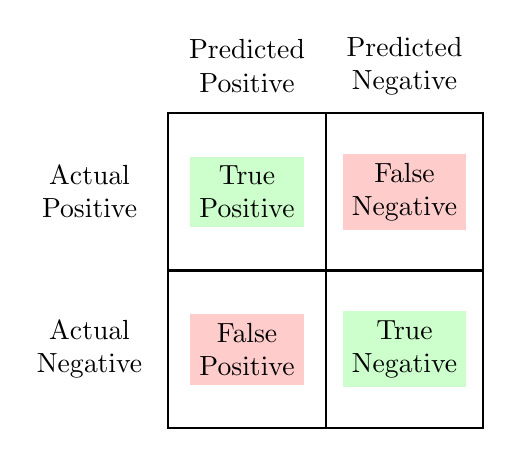
\begin{tikzpicture}
            % Draw the grid
    \draw[thick] (0,0) rectangle (4,4);
    \draw[thick] (2,0) -- (2,4);
    \draw[thick] (0,2) -- (4,2);

    % Label the axes
    \node[align=center] at (1,4.6) {Predicted\\Positive};
    \node[align=center] at (3,4.6) {Predicted\\Negative};

    \node[align=center] at (-1, 3) {Actual\\Positive};
    \node[align=center] at (-1, 1) {Actual\\Negative};

    % Label the cells
    \node[align=center, fill=green!20] at (1,3) {True\\Positive};
    \node[align=center, fill=red!20] at (1,1) {False\\Positive};
    \node[align=center, fill=red!20] at (3,3) {False\\Negative};
    \node[align=center, fill=green!20] at (3,1) {True\\Negative};
    \end{tikzpicture}

\end{center}
    \caption[Binary classification confusion matrix]{Figure showing the binary classification confusion matrix, denoting the four possible combinations created by the ground truth and predicted class. Green cells denote correct predictions, while red cells denote wrong predictions.}
\label{fig:confusion}
\end{figure}

With these possibilities defined, we can begin to gain a clearer picture of the performance of a model.

\noindent \textbf{Precision and Recall}

\noindent Precision is the share of positive predictions that were actually positive. With a high false positive rate, we have a low precision, which means that the model is erroneously flagging many negative classes as positive. In an \ac{ood} detection setting, a model which flags many \ac{id} samples as \ac{ood} would have a low precision, if we treat \ac{ood} samples as the positive class.

Recall is the share of actual positive samples that were predicted positive. Recall tells us how many of positive samples we missed. In and \ac{ood} detection context, a model which lets many \ac{ood} samples slip by undetected will have a low recall score.

Precision and recall are often used together because evaluate the model in different ways that complement each other. If a model has both high precision and high recall, it does not erroneously flag many negative classes as positive, nor does it miss many positive classes.

\noindent \textbf{Sensitivity and Specificity}

\noindent Sensitivity and specificity is another pair of metrics that is commonly used for evaluating binary classification. Sensitivity is equivalent to recall; the share of positive samples that were correctly predicted as positive. Specificity is the share of the negative samples that were correctly predicted as negative. Sensitivity and specificity are also known as \ac{tpr} and {\it True Negative Rate}.

\subsubsection{Threshold Independent Metrics}

The previous metrics are a clear improvement over simply using accuracy. However, they still have the problem that they are all dependent on what threshold one sets when predicting something to be a negative or positive class. Thus, it becomes harder to compare different models by using these metrics. Indeed, by simply increasing the threshold of any classifier, we can increase the true negative rate. Similarly, by decreasing the threshold, we can increase the true positive rate.\\

\noindent \textbf{Area under Receiver Operating Characteristic}:

\noindent \ac{auroc} remedies this problem by looking at all possible thresholds, and calculating the \ac{tpr} (equivalent to sensitivity, recall), and the \ac{fpr} (equivalent to $1 -$ specificity) for each possible threshold. With these values calculated, we can plot each point on a graph, giving us an \ac{roc} plot. Figure \ref{fig:auroc} shows this plot, for three different models.

\begin{figure}[H]
    \begin{center}
        %% Creator: Matplotlib, PGF backend
%%
%% To include the figure in your LaTeX document, write
%%   \input{<filename>.pgf}
%%
%% Make sure the required packages are loaded in your preamble
%%   \usepackage{pgf}
%%
%% Also ensure that all the required font packages are loaded; for instance,
%% the lmodern package is sometimes necessary when using math font.
%%   \usepackage{lmodern}
%%
%% Figures using additional raster images can only be included by \input if
%% they are in the same directory as the main LaTeX file. For loading figures
%% from other directories you can use the `import` package
%%   \usepackage{import}
%%
%% and then include the figures with
%%   \import{<path to file>}{<filename>.pgf}
%%
%% Matplotlib used the following preamble
%%   \def\mathdefault#1{#1}
%%   \everymath=\expandafter{\the\everymath\displaystyle}
%%   \IfFileExists{scrextend.sty}{
%%     \usepackage[fontsize=10.000000pt]{scrextend}
%%   }{
%%     \renewcommand{\normalsize}{\fontsize{10.000000}{12.000000}\selectfont}
%%     \normalsize
%%   }
%%   
%%   \makeatletter\@ifpackageloaded{underscore}{}{\usepackage[strings]{underscore}}\makeatother
%%
\begingroup%
\makeatletter%
\begin{pgfpicture}%
\pgfpathrectangle{\pgfpointorigin}{\pgfqpoint{6.400000in}{4.800000in}}%
\pgfusepath{use as bounding box, clip}%
\begin{pgfscope}%
\pgfsetbuttcap%
\pgfsetmiterjoin%
\definecolor{currentfill}{rgb}{1.000000,1.000000,1.000000}%
\pgfsetfillcolor{currentfill}%
\pgfsetlinewidth{0.000000pt}%
\definecolor{currentstroke}{rgb}{1.000000,1.000000,1.000000}%
\pgfsetstrokecolor{currentstroke}%
\pgfsetdash{}{0pt}%
\pgfpathmoveto{\pgfqpoint{0.000000in}{0.000000in}}%
\pgfpathlineto{\pgfqpoint{6.400000in}{0.000000in}}%
\pgfpathlineto{\pgfqpoint{6.400000in}{4.800000in}}%
\pgfpathlineto{\pgfqpoint{0.000000in}{4.800000in}}%
\pgfpathlineto{\pgfqpoint{0.000000in}{0.000000in}}%
\pgfpathclose%
\pgfusepath{fill}%
\end{pgfscope}%
\begin{pgfscope}%
\pgfsetbuttcap%
\pgfsetmiterjoin%
\definecolor{currentfill}{rgb}{1.000000,1.000000,1.000000}%
\pgfsetfillcolor{currentfill}%
\pgfsetlinewidth{0.000000pt}%
\definecolor{currentstroke}{rgb}{0.000000,0.000000,0.000000}%
\pgfsetstrokecolor{currentstroke}%
\pgfsetstrokeopacity{0.000000}%
\pgfsetdash{}{0pt}%
\pgfpathmoveto{\pgfqpoint{0.800000in}{0.528000in}}%
\pgfpathlineto{\pgfqpoint{5.760000in}{0.528000in}}%
\pgfpathlineto{\pgfqpoint{5.760000in}{4.224000in}}%
\pgfpathlineto{\pgfqpoint{0.800000in}{4.224000in}}%
\pgfpathlineto{\pgfqpoint{0.800000in}{0.528000in}}%
\pgfpathclose%
\pgfusepath{fill}%
\end{pgfscope}%
\begin{pgfscope}%
\pgfpathrectangle{\pgfqpoint{0.800000in}{0.528000in}}{\pgfqpoint{4.960000in}{3.696000in}}%
\pgfusepath{clip}%
\pgfsetrectcap%
\pgfsetroundjoin%
\pgfsetlinewidth{0.803000pt}%
\definecolor{currentstroke}{rgb}{0.690196,0.690196,0.690196}%
\pgfsetstrokecolor{currentstroke}%
\pgfsetdash{}{0pt}%
\pgfpathmoveto{\pgfqpoint{0.800000in}{0.528000in}}%
\pgfpathlineto{\pgfqpoint{0.800000in}{4.224000in}}%
\pgfusepath{stroke}%
\end{pgfscope}%
\begin{pgfscope}%
\pgfsetbuttcap%
\pgfsetroundjoin%
\definecolor{currentfill}{rgb}{0.000000,0.000000,0.000000}%
\pgfsetfillcolor{currentfill}%
\pgfsetlinewidth{0.803000pt}%
\definecolor{currentstroke}{rgb}{0.000000,0.000000,0.000000}%
\pgfsetstrokecolor{currentstroke}%
\pgfsetdash{}{0pt}%
\pgfsys@defobject{currentmarker}{\pgfqpoint{0.000000in}{-0.048611in}}{\pgfqpoint{0.000000in}{0.000000in}}{%
\pgfpathmoveto{\pgfqpoint{0.000000in}{0.000000in}}%
\pgfpathlineto{\pgfqpoint{0.000000in}{-0.048611in}}%
\pgfusepath{stroke,fill}%
}%
\begin{pgfscope}%
\pgfsys@transformshift{0.800000in}{0.528000in}%
\pgfsys@useobject{currentmarker}{}%
\end{pgfscope}%
\end{pgfscope}%
\begin{pgfscope}%
\definecolor{textcolor}{rgb}{0.000000,0.000000,0.000000}%
\pgfsetstrokecolor{textcolor}%
\pgfsetfillcolor{textcolor}%
\pgftext[x=0.800000in,y=0.430778in,,top]{\color{textcolor}{\rmfamily\fontsize{10.000000}{12.000000}\selectfont\catcode`\^=\active\def^{\ifmmode\sp\else\^{}\fi}\catcode`\%=\active\def%{\%}$\mathdefault{0.0}$}}%
\end{pgfscope}%
\begin{pgfscope}%
\pgfpathrectangle{\pgfqpoint{0.800000in}{0.528000in}}{\pgfqpoint{4.960000in}{3.696000in}}%
\pgfusepath{clip}%
\pgfsetrectcap%
\pgfsetroundjoin%
\pgfsetlinewidth{0.803000pt}%
\definecolor{currentstroke}{rgb}{0.690196,0.690196,0.690196}%
\pgfsetstrokecolor{currentstroke}%
\pgfsetdash{}{0pt}%
\pgfpathmoveto{\pgfqpoint{1.792000in}{0.528000in}}%
\pgfpathlineto{\pgfqpoint{1.792000in}{4.224000in}}%
\pgfusepath{stroke}%
\end{pgfscope}%
\begin{pgfscope}%
\pgfsetbuttcap%
\pgfsetroundjoin%
\definecolor{currentfill}{rgb}{0.000000,0.000000,0.000000}%
\pgfsetfillcolor{currentfill}%
\pgfsetlinewidth{0.803000pt}%
\definecolor{currentstroke}{rgb}{0.000000,0.000000,0.000000}%
\pgfsetstrokecolor{currentstroke}%
\pgfsetdash{}{0pt}%
\pgfsys@defobject{currentmarker}{\pgfqpoint{0.000000in}{-0.048611in}}{\pgfqpoint{0.000000in}{0.000000in}}{%
\pgfpathmoveto{\pgfqpoint{0.000000in}{0.000000in}}%
\pgfpathlineto{\pgfqpoint{0.000000in}{-0.048611in}}%
\pgfusepath{stroke,fill}%
}%
\begin{pgfscope}%
\pgfsys@transformshift{1.792000in}{0.528000in}%
\pgfsys@useobject{currentmarker}{}%
\end{pgfscope}%
\end{pgfscope}%
\begin{pgfscope}%
\definecolor{textcolor}{rgb}{0.000000,0.000000,0.000000}%
\pgfsetstrokecolor{textcolor}%
\pgfsetfillcolor{textcolor}%
\pgftext[x=1.792000in,y=0.430778in,,top]{\color{textcolor}{\rmfamily\fontsize{10.000000}{12.000000}\selectfont\catcode`\^=\active\def^{\ifmmode\sp\else\^{}\fi}\catcode`\%=\active\def%{\%}$\mathdefault{0.2}$}}%
\end{pgfscope}%
\begin{pgfscope}%
\pgfpathrectangle{\pgfqpoint{0.800000in}{0.528000in}}{\pgfqpoint{4.960000in}{3.696000in}}%
\pgfusepath{clip}%
\pgfsetrectcap%
\pgfsetroundjoin%
\pgfsetlinewidth{0.803000pt}%
\definecolor{currentstroke}{rgb}{0.690196,0.690196,0.690196}%
\pgfsetstrokecolor{currentstroke}%
\pgfsetdash{}{0pt}%
\pgfpathmoveto{\pgfqpoint{2.784000in}{0.528000in}}%
\pgfpathlineto{\pgfqpoint{2.784000in}{4.224000in}}%
\pgfusepath{stroke}%
\end{pgfscope}%
\begin{pgfscope}%
\pgfsetbuttcap%
\pgfsetroundjoin%
\definecolor{currentfill}{rgb}{0.000000,0.000000,0.000000}%
\pgfsetfillcolor{currentfill}%
\pgfsetlinewidth{0.803000pt}%
\definecolor{currentstroke}{rgb}{0.000000,0.000000,0.000000}%
\pgfsetstrokecolor{currentstroke}%
\pgfsetdash{}{0pt}%
\pgfsys@defobject{currentmarker}{\pgfqpoint{0.000000in}{-0.048611in}}{\pgfqpoint{0.000000in}{0.000000in}}{%
\pgfpathmoveto{\pgfqpoint{0.000000in}{0.000000in}}%
\pgfpathlineto{\pgfqpoint{0.000000in}{-0.048611in}}%
\pgfusepath{stroke,fill}%
}%
\begin{pgfscope}%
\pgfsys@transformshift{2.784000in}{0.528000in}%
\pgfsys@useobject{currentmarker}{}%
\end{pgfscope}%
\end{pgfscope}%
\begin{pgfscope}%
\definecolor{textcolor}{rgb}{0.000000,0.000000,0.000000}%
\pgfsetstrokecolor{textcolor}%
\pgfsetfillcolor{textcolor}%
\pgftext[x=2.784000in,y=0.430778in,,top]{\color{textcolor}{\rmfamily\fontsize{10.000000}{12.000000}\selectfont\catcode`\^=\active\def^{\ifmmode\sp\else\^{}\fi}\catcode`\%=\active\def%{\%}$\mathdefault{0.4}$}}%
\end{pgfscope}%
\begin{pgfscope}%
\pgfpathrectangle{\pgfqpoint{0.800000in}{0.528000in}}{\pgfqpoint{4.960000in}{3.696000in}}%
\pgfusepath{clip}%
\pgfsetrectcap%
\pgfsetroundjoin%
\pgfsetlinewidth{0.803000pt}%
\definecolor{currentstroke}{rgb}{0.690196,0.690196,0.690196}%
\pgfsetstrokecolor{currentstroke}%
\pgfsetdash{}{0pt}%
\pgfpathmoveto{\pgfqpoint{3.776000in}{0.528000in}}%
\pgfpathlineto{\pgfqpoint{3.776000in}{4.224000in}}%
\pgfusepath{stroke}%
\end{pgfscope}%
\begin{pgfscope}%
\pgfsetbuttcap%
\pgfsetroundjoin%
\definecolor{currentfill}{rgb}{0.000000,0.000000,0.000000}%
\pgfsetfillcolor{currentfill}%
\pgfsetlinewidth{0.803000pt}%
\definecolor{currentstroke}{rgb}{0.000000,0.000000,0.000000}%
\pgfsetstrokecolor{currentstroke}%
\pgfsetdash{}{0pt}%
\pgfsys@defobject{currentmarker}{\pgfqpoint{0.000000in}{-0.048611in}}{\pgfqpoint{0.000000in}{0.000000in}}{%
\pgfpathmoveto{\pgfqpoint{0.000000in}{0.000000in}}%
\pgfpathlineto{\pgfqpoint{0.000000in}{-0.048611in}}%
\pgfusepath{stroke,fill}%
}%
\begin{pgfscope}%
\pgfsys@transformshift{3.776000in}{0.528000in}%
\pgfsys@useobject{currentmarker}{}%
\end{pgfscope}%
\end{pgfscope}%
\begin{pgfscope}%
\definecolor{textcolor}{rgb}{0.000000,0.000000,0.000000}%
\pgfsetstrokecolor{textcolor}%
\pgfsetfillcolor{textcolor}%
\pgftext[x=3.776000in,y=0.430778in,,top]{\color{textcolor}{\rmfamily\fontsize{10.000000}{12.000000}\selectfont\catcode`\^=\active\def^{\ifmmode\sp\else\^{}\fi}\catcode`\%=\active\def%{\%}$\mathdefault{0.6}$}}%
\end{pgfscope}%
\begin{pgfscope}%
\pgfpathrectangle{\pgfqpoint{0.800000in}{0.528000in}}{\pgfqpoint{4.960000in}{3.696000in}}%
\pgfusepath{clip}%
\pgfsetrectcap%
\pgfsetroundjoin%
\pgfsetlinewidth{0.803000pt}%
\definecolor{currentstroke}{rgb}{0.690196,0.690196,0.690196}%
\pgfsetstrokecolor{currentstroke}%
\pgfsetdash{}{0pt}%
\pgfpathmoveto{\pgfqpoint{4.768000in}{0.528000in}}%
\pgfpathlineto{\pgfqpoint{4.768000in}{4.224000in}}%
\pgfusepath{stroke}%
\end{pgfscope}%
\begin{pgfscope}%
\pgfsetbuttcap%
\pgfsetroundjoin%
\definecolor{currentfill}{rgb}{0.000000,0.000000,0.000000}%
\pgfsetfillcolor{currentfill}%
\pgfsetlinewidth{0.803000pt}%
\definecolor{currentstroke}{rgb}{0.000000,0.000000,0.000000}%
\pgfsetstrokecolor{currentstroke}%
\pgfsetdash{}{0pt}%
\pgfsys@defobject{currentmarker}{\pgfqpoint{0.000000in}{-0.048611in}}{\pgfqpoint{0.000000in}{0.000000in}}{%
\pgfpathmoveto{\pgfqpoint{0.000000in}{0.000000in}}%
\pgfpathlineto{\pgfqpoint{0.000000in}{-0.048611in}}%
\pgfusepath{stroke,fill}%
}%
\begin{pgfscope}%
\pgfsys@transformshift{4.768000in}{0.528000in}%
\pgfsys@useobject{currentmarker}{}%
\end{pgfscope}%
\end{pgfscope}%
\begin{pgfscope}%
\definecolor{textcolor}{rgb}{0.000000,0.000000,0.000000}%
\pgfsetstrokecolor{textcolor}%
\pgfsetfillcolor{textcolor}%
\pgftext[x=4.768000in,y=0.430778in,,top]{\color{textcolor}{\rmfamily\fontsize{10.000000}{12.000000}\selectfont\catcode`\^=\active\def^{\ifmmode\sp\else\^{}\fi}\catcode`\%=\active\def%{\%}$\mathdefault{0.8}$}}%
\end{pgfscope}%
\begin{pgfscope}%
\pgfpathrectangle{\pgfqpoint{0.800000in}{0.528000in}}{\pgfqpoint{4.960000in}{3.696000in}}%
\pgfusepath{clip}%
\pgfsetrectcap%
\pgfsetroundjoin%
\pgfsetlinewidth{0.803000pt}%
\definecolor{currentstroke}{rgb}{0.690196,0.690196,0.690196}%
\pgfsetstrokecolor{currentstroke}%
\pgfsetdash{}{0pt}%
\pgfpathmoveto{\pgfqpoint{5.760000in}{0.528000in}}%
\pgfpathlineto{\pgfqpoint{5.760000in}{4.224000in}}%
\pgfusepath{stroke}%
\end{pgfscope}%
\begin{pgfscope}%
\pgfsetbuttcap%
\pgfsetroundjoin%
\definecolor{currentfill}{rgb}{0.000000,0.000000,0.000000}%
\pgfsetfillcolor{currentfill}%
\pgfsetlinewidth{0.803000pt}%
\definecolor{currentstroke}{rgb}{0.000000,0.000000,0.000000}%
\pgfsetstrokecolor{currentstroke}%
\pgfsetdash{}{0pt}%
\pgfsys@defobject{currentmarker}{\pgfqpoint{0.000000in}{-0.048611in}}{\pgfqpoint{0.000000in}{0.000000in}}{%
\pgfpathmoveto{\pgfqpoint{0.000000in}{0.000000in}}%
\pgfpathlineto{\pgfqpoint{0.000000in}{-0.048611in}}%
\pgfusepath{stroke,fill}%
}%
\begin{pgfscope}%
\pgfsys@transformshift{5.760000in}{0.528000in}%
\pgfsys@useobject{currentmarker}{}%
\end{pgfscope}%
\end{pgfscope}%
\begin{pgfscope}%
\definecolor{textcolor}{rgb}{0.000000,0.000000,0.000000}%
\pgfsetstrokecolor{textcolor}%
\pgfsetfillcolor{textcolor}%
\pgftext[x=5.760000in,y=0.430778in,,top]{\color{textcolor}{\rmfamily\fontsize{10.000000}{12.000000}\selectfont\catcode`\^=\active\def^{\ifmmode\sp\else\^{}\fi}\catcode`\%=\active\def%{\%}$\mathdefault{1.0}$}}%
\end{pgfscope}%
\begin{pgfscope}%
\definecolor{textcolor}{rgb}{0.000000,0.000000,0.000000}%
\pgfsetstrokecolor{textcolor}%
\pgfsetfillcolor{textcolor}%
\pgftext[x=3.280000in,y=0.251766in,,top]{\color{textcolor}{\rmfamily\fontsize{10.000000}{12.000000}\selectfont\catcode`\^=\active\def^{\ifmmode\sp\else\^{}\fi}\catcode`\%=\active\def%{\%}False Positive Rate (FPR)}}%
\end{pgfscope}%
\begin{pgfscope}%
\pgfpathrectangle{\pgfqpoint{0.800000in}{0.528000in}}{\pgfqpoint{4.960000in}{3.696000in}}%
\pgfusepath{clip}%
\pgfsetrectcap%
\pgfsetroundjoin%
\pgfsetlinewidth{0.803000pt}%
\definecolor{currentstroke}{rgb}{0.690196,0.690196,0.690196}%
\pgfsetstrokecolor{currentstroke}%
\pgfsetdash{}{0pt}%
\pgfpathmoveto{\pgfqpoint{0.800000in}{0.528000in}}%
\pgfpathlineto{\pgfqpoint{5.760000in}{0.528000in}}%
\pgfusepath{stroke}%
\end{pgfscope}%
\begin{pgfscope}%
\pgfsetbuttcap%
\pgfsetroundjoin%
\definecolor{currentfill}{rgb}{0.000000,0.000000,0.000000}%
\pgfsetfillcolor{currentfill}%
\pgfsetlinewidth{0.803000pt}%
\definecolor{currentstroke}{rgb}{0.000000,0.000000,0.000000}%
\pgfsetstrokecolor{currentstroke}%
\pgfsetdash{}{0pt}%
\pgfsys@defobject{currentmarker}{\pgfqpoint{-0.048611in}{0.000000in}}{\pgfqpoint{-0.000000in}{0.000000in}}{%
\pgfpathmoveto{\pgfqpoint{-0.000000in}{0.000000in}}%
\pgfpathlineto{\pgfqpoint{-0.048611in}{0.000000in}}%
\pgfusepath{stroke,fill}%
}%
\begin{pgfscope}%
\pgfsys@transformshift{0.800000in}{0.528000in}%
\pgfsys@useobject{currentmarker}{}%
\end{pgfscope}%
\end{pgfscope}%
\begin{pgfscope}%
\definecolor{textcolor}{rgb}{0.000000,0.000000,0.000000}%
\pgfsetstrokecolor{textcolor}%
\pgfsetfillcolor{textcolor}%
\pgftext[x=0.525308in, y=0.479775in, left, base]{\color{textcolor}{\rmfamily\fontsize{10.000000}{12.000000}\selectfont\catcode`\^=\active\def^{\ifmmode\sp\else\^{}\fi}\catcode`\%=\active\def%{\%}$\mathdefault{0.0}$}}%
\end{pgfscope}%
\begin{pgfscope}%
\pgfpathrectangle{\pgfqpoint{0.800000in}{0.528000in}}{\pgfqpoint{4.960000in}{3.696000in}}%
\pgfusepath{clip}%
\pgfsetrectcap%
\pgfsetroundjoin%
\pgfsetlinewidth{0.803000pt}%
\definecolor{currentstroke}{rgb}{0.690196,0.690196,0.690196}%
\pgfsetstrokecolor{currentstroke}%
\pgfsetdash{}{0pt}%
\pgfpathmoveto{\pgfqpoint{0.800000in}{1.267200in}}%
\pgfpathlineto{\pgfqpoint{5.760000in}{1.267200in}}%
\pgfusepath{stroke}%
\end{pgfscope}%
\begin{pgfscope}%
\pgfsetbuttcap%
\pgfsetroundjoin%
\definecolor{currentfill}{rgb}{0.000000,0.000000,0.000000}%
\pgfsetfillcolor{currentfill}%
\pgfsetlinewidth{0.803000pt}%
\definecolor{currentstroke}{rgb}{0.000000,0.000000,0.000000}%
\pgfsetstrokecolor{currentstroke}%
\pgfsetdash{}{0pt}%
\pgfsys@defobject{currentmarker}{\pgfqpoint{-0.048611in}{0.000000in}}{\pgfqpoint{-0.000000in}{0.000000in}}{%
\pgfpathmoveto{\pgfqpoint{-0.000000in}{0.000000in}}%
\pgfpathlineto{\pgfqpoint{-0.048611in}{0.000000in}}%
\pgfusepath{stroke,fill}%
}%
\begin{pgfscope}%
\pgfsys@transformshift{0.800000in}{1.267200in}%
\pgfsys@useobject{currentmarker}{}%
\end{pgfscope}%
\end{pgfscope}%
\begin{pgfscope}%
\definecolor{textcolor}{rgb}{0.000000,0.000000,0.000000}%
\pgfsetstrokecolor{textcolor}%
\pgfsetfillcolor{textcolor}%
\pgftext[x=0.525308in, y=1.218975in, left, base]{\color{textcolor}{\rmfamily\fontsize{10.000000}{12.000000}\selectfont\catcode`\^=\active\def^{\ifmmode\sp\else\^{}\fi}\catcode`\%=\active\def%{\%}$\mathdefault{0.2}$}}%
\end{pgfscope}%
\begin{pgfscope}%
\pgfpathrectangle{\pgfqpoint{0.800000in}{0.528000in}}{\pgfqpoint{4.960000in}{3.696000in}}%
\pgfusepath{clip}%
\pgfsetrectcap%
\pgfsetroundjoin%
\pgfsetlinewidth{0.803000pt}%
\definecolor{currentstroke}{rgb}{0.690196,0.690196,0.690196}%
\pgfsetstrokecolor{currentstroke}%
\pgfsetdash{}{0pt}%
\pgfpathmoveto{\pgfqpoint{0.800000in}{2.006400in}}%
\pgfpathlineto{\pgfqpoint{5.760000in}{2.006400in}}%
\pgfusepath{stroke}%
\end{pgfscope}%
\begin{pgfscope}%
\pgfsetbuttcap%
\pgfsetroundjoin%
\definecolor{currentfill}{rgb}{0.000000,0.000000,0.000000}%
\pgfsetfillcolor{currentfill}%
\pgfsetlinewidth{0.803000pt}%
\definecolor{currentstroke}{rgb}{0.000000,0.000000,0.000000}%
\pgfsetstrokecolor{currentstroke}%
\pgfsetdash{}{0pt}%
\pgfsys@defobject{currentmarker}{\pgfqpoint{-0.048611in}{0.000000in}}{\pgfqpoint{-0.000000in}{0.000000in}}{%
\pgfpathmoveto{\pgfqpoint{-0.000000in}{0.000000in}}%
\pgfpathlineto{\pgfqpoint{-0.048611in}{0.000000in}}%
\pgfusepath{stroke,fill}%
}%
\begin{pgfscope}%
\pgfsys@transformshift{0.800000in}{2.006400in}%
\pgfsys@useobject{currentmarker}{}%
\end{pgfscope}%
\end{pgfscope}%
\begin{pgfscope}%
\definecolor{textcolor}{rgb}{0.000000,0.000000,0.000000}%
\pgfsetstrokecolor{textcolor}%
\pgfsetfillcolor{textcolor}%
\pgftext[x=0.525308in, y=1.958175in, left, base]{\color{textcolor}{\rmfamily\fontsize{10.000000}{12.000000}\selectfont\catcode`\^=\active\def^{\ifmmode\sp\else\^{}\fi}\catcode`\%=\active\def%{\%}$\mathdefault{0.4}$}}%
\end{pgfscope}%
\begin{pgfscope}%
\pgfpathrectangle{\pgfqpoint{0.800000in}{0.528000in}}{\pgfqpoint{4.960000in}{3.696000in}}%
\pgfusepath{clip}%
\pgfsetrectcap%
\pgfsetroundjoin%
\pgfsetlinewidth{0.803000pt}%
\definecolor{currentstroke}{rgb}{0.690196,0.690196,0.690196}%
\pgfsetstrokecolor{currentstroke}%
\pgfsetdash{}{0pt}%
\pgfpathmoveto{\pgfqpoint{0.800000in}{2.745600in}}%
\pgfpathlineto{\pgfqpoint{5.760000in}{2.745600in}}%
\pgfusepath{stroke}%
\end{pgfscope}%
\begin{pgfscope}%
\pgfsetbuttcap%
\pgfsetroundjoin%
\definecolor{currentfill}{rgb}{0.000000,0.000000,0.000000}%
\pgfsetfillcolor{currentfill}%
\pgfsetlinewidth{0.803000pt}%
\definecolor{currentstroke}{rgb}{0.000000,0.000000,0.000000}%
\pgfsetstrokecolor{currentstroke}%
\pgfsetdash{}{0pt}%
\pgfsys@defobject{currentmarker}{\pgfqpoint{-0.048611in}{0.000000in}}{\pgfqpoint{-0.000000in}{0.000000in}}{%
\pgfpathmoveto{\pgfqpoint{-0.000000in}{0.000000in}}%
\pgfpathlineto{\pgfqpoint{-0.048611in}{0.000000in}}%
\pgfusepath{stroke,fill}%
}%
\begin{pgfscope}%
\pgfsys@transformshift{0.800000in}{2.745600in}%
\pgfsys@useobject{currentmarker}{}%
\end{pgfscope}%
\end{pgfscope}%
\begin{pgfscope}%
\definecolor{textcolor}{rgb}{0.000000,0.000000,0.000000}%
\pgfsetstrokecolor{textcolor}%
\pgfsetfillcolor{textcolor}%
\pgftext[x=0.525308in, y=2.697375in, left, base]{\color{textcolor}{\rmfamily\fontsize{10.000000}{12.000000}\selectfont\catcode`\^=\active\def^{\ifmmode\sp\else\^{}\fi}\catcode`\%=\active\def%{\%}$\mathdefault{0.6}$}}%
\end{pgfscope}%
\begin{pgfscope}%
\pgfpathrectangle{\pgfqpoint{0.800000in}{0.528000in}}{\pgfqpoint{4.960000in}{3.696000in}}%
\pgfusepath{clip}%
\pgfsetrectcap%
\pgfsetroundjoin%
\pgfsetlinewidth{0.803000pt}%
\definecolor{currentstroke}{rgb}{0.690196,0.690196,0.690196}%
\pgfsetstrokecolor{currentstroke}%
\pgfsetdash{}{0pt}%
\pgfpathmoveto{\pgfqpoint{0.800000in}{3.484800in}}%
\pgfpathlineto{\pgfqpoint{5.760000in}{3.484800in}}%
\pgfusepath{stroke}%
\end{pgfscope}%
\begin{pgfscope}%
\pgfsetbuttcap%
\pgfsetroundjoin%
\definecolor{currentfill}{rgb}{0.000000,0.000000,0.000000}%
\pgfsetfillcolor{currentfill}%
\pgfsetlinewidth{0.803000pt}%
\definecolor{currentstroke}{rgb}{0.000000,0.000000,0.000000}%
\pgfsetstrokecolor{currentstroke}%
\pgfsetdash{}{0pt}%
\pgfsys@defobject{currentmarker}{\pgfqpoint{-0.048611in}{0.000000in}}{\pgfqpoint{-0.000000in}{0.000000in}}{%
\pgfpathmoveto{\pgfqpoint{-0.000000in}{0.000000in}}%
\pgfpathlineto{\pgfqpoint{-0.048611in}{0.000000in}}%
\pgfusepath{stroke,fill}%
}%
\begin{pgfscope}%
\pgfsys@transformshift{0.800000in}{3.484800in}%
\pgfsys@useobject{currentmarker}{}%
\end{pgfscope}%
\end{pgfscope}%
\begin{pgfscope}%
\definecolor{textcolor}{rgb}{0.000000,0.000000,0.000000}%
\pgfsetstrokecolor{textcolor}%
\pgfsetfillcolor{textcolor}%
\pgftext[x=0.525308in, y=3.436575in, left, base]{\color{textcolor}{\rmfamily\fontsize{10.000000}{12.000000}\selectfont\catcode`\^=\active\def^{\ifmmode\sp\else\^{}\fi}\catcode`\%=\active\def%{\%}$\mathdefault{0.8}$}}%
\end{pgfscope}%
\begin{pgfscope}%
\pgfpathrectangle{\pgfqpoint{0.800000in}{0.528000in}}{\pgfqpoint{4.960000in}{3.696000in}}%
\pgfusepath{clip}%
\pgfsetrectcap%
\pgfsetroundjoin%
\pgfsetlinewidth{0.803000pt}%
\definecolor{currentstroke}{rgb}{0.690196,0.690196,0.690196}%
\pgfsetstrokecolor{currentstroke}%
\pgfsetdash{}{0pt}%
\pgfpathmoveto{\pgfqpoint{0.800000in}{4.224000in}}%
\pgfpathlineto{\pgfqpoint{5.760000in}{4.224000in}}%
\pgfusepath{stroke}%
\end{pgfscope}%
\begin{pgfscope}%
\pgfsetbuttcap%
\pgfsetroundjoin%
\definecolor{currentfill}{rgb}{0.000000,0.000000,0.000000}%
\pgfsetfillcolor{currentfill}%
\pgfsetlinewidth{0.803000pt}%
\definecolor{currentstroke}{rgb}{0.000000,0.000000,0.000000}%
\pgfsetstrokecolor{currentstroke}%
\pgfsetdash{}{0pt}%
\pgfsys@defobject{currentmarker}{\pgfqpoint{-0.048611in}{0.000000in}}{\pgfqpoint{-0.000000in}{0.000000in}}{%
\pgfpathmoveto{\pgfqpoint{-0.000000in}{0.000000in}}%
\pgfpathlineto{\pgfqpoint{-0.048611in}{0.000000in}}%
\pgfusepath{stroke,fill}%
}%
\begin{pgfscope}%
\pgfsys@transformshift{0.800000in}{4.224000in}%
\pgfsys@useobject{currentmarker}{}%
\end{pgfscope}%
\end{pgfscope}%
\begin{pgfscope}%
\definecolor{textcolor}{rgb}{0.000000,0.000000,0.000000}%
\pgfsetstrokecolor{textcolor}%
\pgfsetfillcolor{textcolor}%
\pgftext[x=0.525308in, y=4.175775in, left, base]{\color{textcolor}{\rmfamily\fontsize{10.000000}{12.000000}\selectfont\catcode`\^=\active\def^{\ifmmode\sp\else\^{}\fi}\catcode`\%=\active\def%{\%}$\mathdefault{1.0}$}}%
\end{pgfscope}%
\begin{pgfscope}%
\definecolor{textcolor}{rgb}{0.000000,0.000000,0.000000}%
\pgfsetstrokecolor{textcolor}%
\pgfsetfillcolor{textcolor}%
\pgftext[x=0.469752in,y=2.376000in,,bottom,rotate=90.000000]{\color{textcolor}{\rmfamily\fontsize{10.000000}{12.000000}\selectfont\catcode`\^=\active\def^{\ifmmode\sp\else\^{}\fi}\catcode`\%=\active\def%{\%}True Positive Rate (TPR)}}%
\end{pgfscope}%
\begin{pgfscope}%
\pgfpathrectangle{\pgfqpoint{0.800000in}{0.528000in}}{\pgfqpoint{4.960000in}{3.696000in}}%
\pgfusepath{clip}%
\pgfsetrectcap%
\pgfsetroundjoin%
\pgfsetlinewidth{1.505625pt}%
\definecolor{currentstroke}{rgb}{0.000000,0.501961,0.000000}%
\pgfsetstrokecolor{currentstroke}%
\pgfsetdash{}{0pt}%
\pgfpathmoveto{\pgfqpoint{0.800000in}{0.528000in}}%
\pgfpathlineto{\pgfqpoint{0.800000in}{0.564960in}}%
\pgfpathlineto{\pgfqpoint{0.800000in}{1.415040in}}%
\pgfpathlineto{\pgfqpoint{0.849600in}{1.415040in}}%
\pgfpathlineto{\pgfqpoint{0.849600in}{3.041280in}}%
\pgfpathlineto{\pgfqpoint{0.899200in}{3.041280in}}%
\pgfpathlineto{\pgfqpoint{0.899200in}{3.595680in}}%
\pgfpathlineto{\pgfqpoint{0.948800in}{3.595680in}}%
\pgfpathlineto{\pgfqpoint{0.948800in}{3.669600in}}%
\pgfpathlineto{\pgfqpoint{0.998400in}{3.669600in}}%
\pgfpathlineto{\pgfqpoint{0.998400in}{3.706560in}}%
\pgfpathlineto{\pgfqpoint{1.048000in}{3.706560in}}%
\pgfpathlineto{\pgfqpoint{1.048000in}{3.891360in}}%
\pgfpathlineto{\pgfqpoint{1.246400in}{3.891360in}}%
\pgfpathlineto{\pgfqpoint{1.246400in}{4.039200in}}%
\pgfpathlineto{\pgfqpoint{1.296000in}{4.039200in}}%
\pgfpathlineto{\pgfqpoint{1.296000in}{4.076160in}}%
\pgfpathlineto{\pgfqpoint{1.593600in}{4.076160in}}%
\pgfpathlineto{\pgfqpoint{1.593600in}{4.113120in}}%
\pgfpathlineto{\pgfqpoint{1.891200in}{4.113120in}}%
\pgfpathlineto{\pgfqpoint{1.891200in}{4.150080in}}%
\pgfpathlineto{\pgfqpoint{2.288000in}{4.150080in}}%
\pgfpathlineto{\pgfqpoint{2.288000in}{4.187040in}}%
\pgfpathlineto{\pgfqpoint{2.536000in}{4.187040in}}%
\pgfpathlineto{\pgfqpoint{2.536000in}{4.224000in}}%
\pgfpathlineto{\pgfqpoint{5.760000in}{4.224000in}}%
\pgfusepath{stroke}%
\end{pgfscope}%
\begin{pgfscope}%
\pgfpathrectangle{\pgfqpoint{0.800000in}{0.528000in}}{\pgfqpoint{4.960000in}{3.696000in}}%
\pgfusepath{clip}%
\pgfsetrectcap%
\pgfsetroundjoin%
\pgfsetlinewidth{1.505625pt}%
\definecolor{currentstroke}{rgb}{0.000000,0.000000,1.000000}%
\pgfsetstrokecolor{currentstroke}%
\pgfsetdash{}{0pt}%
\pgfpathmoveto{\pgfqpoint{0.800000in}{0.528000in}}%
\pgfpathlineto{\pgfqpoint{0.849600in}{0.528000in}}%
\pgfpathlineto{\pgfqpoint{0.849600in}{1.008480in}}%
\pgfpathlineto{\pgfqpoint{0.899200in}{1.008480in}}%
\pgfpathlineto{\pgfqpoint{0.899200in}{1.119360in}}%
\pgfpathlineto{\pgfqpoint{0.948800in}{1.119360in}}%
\pgfpathlineto{\pgfqpoint{0.948800in}{1.267200in}}%
\pgfpathlineto{\pgfqpoint{0.998400in}{1.267200in}}%
\pgfpathlineto{\pgfqpoint{0.998400in}{1.378080in}}%
\pgfpathlineto{\pgfqpoint{1.048000in}{1.378080in}}%
\pgfpathlineto{\pgfqpoint{1.048000in}{1.415040in}}%
\pgfpathlineto{\pgfqpoint{1.097600in}{1.415040in}}%
\pgfpathlineto{\pgfqpoint{1.097600in}{1.525920in}}%
\pgfpathlineto{\pgfqpoint{1.147200in}{1.525920in}}%
\pgfpathlineto{\pgfqpoint{1.147200in}{1.821600in}}%
\pgfpathlineto{\pgfqpoint{1.196800in}{1.821600in}}%
\pgfpathlineto{\pgfqpoint{1.196800in}{1.895520in}}%
\pgfpathlineto{\pgfqpoint{1.246400in}{1.895520in}}%
\pgfpathlineto{\pgfqpoint{1.246400in}{1.932480in}}%
\pgfpathlineto{\pgfqpoint{1.296000in}{1.932480in}}%
\pgfpathlineto{\pgfqpoint{1.296000in}{2.043360in}}%
\pgfpathlineto{\pgfqpoint{1.444800in}{2.043360in}}%
\pgfpathlineto{\pgfqpoint{1.444800in}{2.449920in}}%
\pgfpathlineto{\pgfqpoint{1.494400in}{2.449920in}}%
\pgfpathlineto{\pgfqpoint{1.494400in}{2.634720in}}%
\pgfpathlineto{\pgfqpoint{1.544000in}{2.634720in}}%
\pgfpathlineto{\pgfqpoint{1.544000in}{2.930400in}}%
\pgfpathlineto{\pgfqpoint{1.593600in}{2.930400in}}%
\pgfpathlineto{\pgfqpoint{1.593600in}{3.041280in}}%
\pgfpathlineto{\pgfqpoint{1.643200in}{3.041280in}}%
\pgfpathlineto{\pgfqpoint{1.643200in}{3.078240in}}%
\pgfpathlineto{\pgfqpoint{1.692800in}{3.078240in}}%
\pgfpathlineto{\pgfqpoint{1.692800in}{3.115200in}}%
\pgfpathlineto{\pgfqpoint{1.841600in}{3.115200in}}%
\pgfpathlineto{\pgfqpoint{1.841600in}{3.189120in}}%
\pgfpathlineto{\pgfqpoint{2.040000in}{3.189120in}}%
\pgfpathlineto{\pgfqpoint{2.040000in}{3.226080in}}%
\pgfpathlineto{\pgfqpoint{2.139200in}{3.226080in}}%
\pgfpathlineto{\pgfqpoint{2.139200in}{3.336960in}}%
\pgfpathlineto{\pgfqpoint{2.188800in}{3.336960in}}%
\pgfpathlineto{\pgfqpoint{2.188800in}{3.410880in}}%
\pgfpathlineto{\pgfqpoint{2.238400in}{3.410880in}}%
\pgfpathlineto{\pgfqpoint{2.238400in}{3.484800in}}%
\pgfpathlineto{\pgfqpoint{2.288000in}{3.484800in}}%
\pgfpathlineto{\pgfqpoint{2.288000in}{3.558720in}}%
\pgfpathlineto{\pgfqpoint{2.436800in}{3.558720in}}%
\pgfpathlineto{\pgfqpoint{2.436800in}{3.595680in}}%
\pgfpathlineto{\pgfqpoint{2.486400in}{3.595680in}}%
\pgfpathlineto{\pgfqpoint{2.486400in}{3.632640in}}%
\pgfpathlineto{\pgfqpoint{2.536000in}{3.632640in}}%
\pgfpathlineto{\pgfqpoint{2.536000in}{3.669600in}}%
\pgfpathlineto{\pgfqpoint{2.734400in}{3.669600in}}%
\pgfpathlineto{\pgfqpoint{2.734400in}{3.706560in}}%
\pgfpathlineto{\pgfqpoint{2.932800in}{3.706560in}}%
\pgfpathlineto{\pgfqpoint{2.932800in}{3.780480in}}%
\pgfpathlineto{\pgfqpoint{3.230400in}{3.780480in}}%
\pgfpathlineto{\pgfqpoint{3.230400in}{3.854400in}}%
\pgfpathlineto{\pgfqpoint{3.280000in}{3.854400in}}%
\pgfpathlineto{\pgfqpoint{3.280000in}{3.891360in}}%
\pgfpathlineto{\pgfqpoint{3.676800in}{3.891360in}}%
\pgfpathlineto{\pgfqpoint{3.676800in}{3.928320in}}%
\pgfpathlineto{\pgfqpoint{3.726400in}{3.928320in}}%
\pgfpathlineto{\pgfqpoint{3.726400in}{3.965280in}}%
\pgfpathlineto{\pgfqpoint{3.825600in}{3.965280in}}%
\pgfpathlineto{\pgfqpoint{3.825600in}{4.002240in}}%
\pgfpathlineto{\pgfqpoint{3.875200in}{4.002240in}}%
\pgfpathlineto{\pgfqpoint{3.875200in}{4.076160in}}%
\pgfpathlineto{\pgfqpoint{3.974400in}{4.076160in}}%
\pgfpathlineto{\pgfqpoint{3.974400in}{4.113120in}}%
\pgfpathlineto{\pgfqpoint{4.172800in}{4.113120in}}%
\pgfpathlineto{\pgfqpoint{4.172800in}{4.150080in}}%
\pgfpathlineto{\pgfqpoint{5.115200in}{4.150080in}}%
\pgfpathlineto{\pgfqpoint{5.115200in}{4.224000in}}%
\pgfpathlineto{\pgfqpoint{5.760000in}{4.224000in}}%
\pgfusepath{stroke}%
\end{pgfscope}%
\begin{pgfscope}%
\pgfpathrectangle{\pgfqpoint{0.800000in}{0.528000in}}{\pgfqpoint{4.960000in}{3.696000in}}%
\pgfusepath{clip}%
\pgfsetbuttcap%
\pgfsetroundjoin%
\pgfsetlinewidth{1.505625pt}%
\definecolor{currentstroke}{rgb}{0.501961,0.501961,0.501961}%
\pgfsetstrokecolor{currentstroke}%
\pgfsetdash{{5.550000pt}{2.400000pt}}{0.000000pt}%
\pgfpathmoveto{\pgfqpoint{0.800000in}{0.528000in}}%
\pgfpathlineto{\pgfqpoint{5.760000in}{4.224000in}}%
\pgfusepath{stroke}%
\end{pgfscope}%
\begin{pgfscope}%
\pgfsetrectcap%
\pgfsetmiterjoin%
\pgfsetlinewidth{0.803000pt}%
\definecolor{currentstroke}{rgb}{0.000000,0.000000,0.000000}%
\pgfsetstrokecolor{currentstroke}%
\pgfsetdash{}{0pt}%
\pgfpathmoveto{\pgfqpoint{0.800000in}{0.528000in}}%
\pgfpathlineto{\pgfqpoint{0.800000in}{4.224000in}}%
\pgfusepath{stroke}%
\end{pgfscope}%
\begin{pgfscope}%
\pgfsetrectcap%
\pgfsetmiterjoin%
\pgfsetlinewidth{0.803000pt}%
\definecolor{currentstroke}{rgb}{0.000000,0.000000,0.000000}%
\pgfsetstrokecolor{currentstroke}%
\pgfsetdash{}{0pt}%
\pgfpathmoveto{\pgfqpoint{5.760000in}{0.528000in}}%
\pgfpathlineto{\pgfqpoint{5.760000in}{4.224000in}}%
\pgfusepath{stroke}%
\end{pgfscope}%
\begin{pgfscope}%
\pgfsetrectcap%
\pgfsetmiterjoin%
\pgfsetlinewidth{0.803000pt}%
\definecolor{currentstroke}{rgb}{0.000000,0.000000,0.000000}%
\pgfsetstrokecolor{currentstroke}%
\pgfsetdash{}{0pt}%
\pgfpathmoveto{\pgfqpoint{0.800000in}{0.528000in}}%
\pgfpathlineto{\pgfqpoint{5.760000in}{0.528000in}}%
\pgfusepath{stroke}%
\end{pgfscope}%
\begin{pgfscope}%
\pgfsetrectcap%
\pgfsetmiterjoin%
\pgfsetlinewidth{0.803000pt}%
\definecolor{currentstroke}{rgb}{0.000000,0.000000,0.000000}%
\pgfsetstrokecolor{currentstroke}%
\pgfsetdash{}{0pt}%
\pgfpathmoveto{\pgfqpoint{0.800000in}{4.224000in}}%
\pgfpathlineto{\pgfqpoint{5.760000in}{4.224000in}}%
\pgfusepath{stroke}%
\end{pgfscope}%
\begin{pgfscope}%
\definecolor{textcolor}{rgb}{0.000000,0.000000,0.000000}%
\pgfsetstrokecolor{textcolor}%
\pgfsetfillcolor{textcolor}%
\pgftext[x=3.280000in,y=4.307333in,,base]{\color{textcolor}{\rmfamily\fontsize{12.000000}{14.400000}\selectfont\catcode`\^=\active\def^{\ifmmode\sp\else\^{}\fi}\catcode`\%=\active\def%{\%}Receiver Operating Characteristic (ROC)}}%
\end{pgfscope}%
\begin{pgfscope}%
\pgfsetbuttcap%
\pgfsetmiterjoin%
\definecolor{currentfill}{rgb}{1.000000,1.000000,1.000000}%
\pgfsetfillcolor{currentfill}%
\pgfsetfillopacity{0.800000}%
\pgfsetlinewidth{1.003750pt}%
\definecolor{currentstroke}{rgb}{0.800000,0.800000,0.800000}%
\pgfsetstrokecolor{currentstroke}%
\pgfsetstrokeopacity{0.800000}%
\pgfsetdash{}{0pt}%
\pgfpathmoveto{\pgfqpoint{4.259613in}{0.597444in}}%
\pgfpathlineto{\pgfqpoint{5.662778in}{0.597444in}}%
\pgfpathquadraticcurveto{\pgfqpoint{5.690556in}{0.597444in}}{\pgfqpoint{5.690556in}{0.625222in}}%
\pgfpathlineto{\pgfqpoint{5.690556in}{1.192352in}}%
\pgfpathquadraticcurveto{\pgfqpoint{5.690556in}{1.220129in}}{\pgfqpoint{5.662778in}{1.220129in}}%
\pgfpathlineto{\pgfqpoint{4.259613in}{1.220129in}}%
\pgfpathquadraticcurveto{\pgfqpoint{4.231835in}{1.220129in}}{\pgfqpoint{4.231835in}{1.192352in}}%
\pgfpathlineto{\pgfqpoint{4.231835in}{0.625222in}}%
\pgfpathquadraticcurveto{\pgfqpoint{4.231835in}{0.597444in}}{\pgfqpoint{4.259613in}{0.597444in}}%
\pgfpathlineto{\pgfqpoint{4.259613in}{0.597444in}}%
\pgfpathclose%
\pgfusepath{stroke,fill}%
\end{pgfscope}%
\begin{pgfscope}%
\pgfsetrectcap%
\pgfsetroundjoin%
\pgfsetlinewidth{1.505625pt}%
\definecolor{currentstroke}{rgb}{0.000000,0.501961,0.000000}%
\pgfsetstrokecolor{currentstroke}%
\pgfsetdash{}{0pt}%
\pgfpathmoveto{\pgfqpoint{4.287390in}{1.115963in}}%
\pgfpathlineto{\pgfqpoint{4.426279in}{1.115963in}}%
\pgfpathlineto{\pgfqpoint{4.565168in}{1.115963in}}%
\pgfusepath{stroke}%
\end{pgfscope}%
\begin{pgfscope}%
\definecolor{textcolor}{rgb}{0.000000,0.000000,0.000000}%
\pgfsetstrokecolor{textcolor}%
\pgfsetfillcolor{textcolor}%
\pgftext[x=4.676279in,y=1.067352in,left,base]{\color{textcolor}{\rmfamily\fontsize{10.000000}{12.000000}\selectfont\catcode`\^=\active\def^{\ifmmode\sp\else\^{}\fi}\catcode`\%=\active\def%{\%}AUROC = 0.97}}%
\end{pgfscope}%
\begin{pgfscope}%
\pgfsetrectcap%
\pgfsetroundjoin%
\pgfsetlinewidth{1.505625pt}%
\definecolor{currentstroke}{rgb}{0.000000,0.000000,1.000000}%
\pgfsetstrokecolor{currentstroke}%
\pgfsetdash{}{0pt}%
\pgfpathmoveto{\pgfqpoint{4.287390in}{0.922290in}}%
\pgfpathlineto{\pgfqpoint{4.426279in}{0.922290in}}%
\pgfpathlineto{\pgfqpoint{4.565168in}{0.922290in}}%
\pgfusepath{stroke}%
\end{pgfscope}%
\begin{pgfscope}%
\definecolor{textcolor}{rgb}{0.000000,0.000000,0.000000}%
\pgfsetstrokecolor{textcolor}%
\pgfsetfillcolor{textcolor}%
\pgftext[x=4.676279in,y=0.873679in,left,base]{\color{textcolor}{\rmfamily\fontsize{10.000000}{12.000000}\selectfont\catcode`\^=\active\def^{\ifmmode\sp\else\^{}\fi}\catcode`\%=\active\def%{\%}AUROC = 0.81}}%
\end{pgfscope}%
\begin{pgfscope}%
\pgfsetbuttcap%
\pgfsetroundjoin%
\pgfsetlinewidth{1.505625pt}%
\definecolor{currentstroke}{rgb}{0.501961,0.501961,0.501961}%
\pgfsetstrokecolor{currentstroke}%
\pgfsetdash{{5.550000pt}{2.400000pt}}{0.000000pt}%
\pgfpathmoveto{\pgfqpoint{4.287390in}{0.728617in}}%
\pgfpathlineto{\pgfqpoint{4.426279in}{0.728617in}}%
\pgfpathlineto{\pgfqpoint{4.565168in}{0.728617in}}%
\pgfusepath{stroke}%
\end{pgfscope}%
\begin{pgfscope}%
\definecolor{textcolor}{rgb}{0.000000,0.000000,0.000000}%
\pgfsetstrokecolor{textcolor}%
\pgfsetfillcolor{textcolor}%
\pgftext[x=4.676279in,y=0.680006in,left,base]{\color{textcolor}{\rmfamily\fontsize{10.000000}{12.000000}\selectfont\catcode`\^=\active\def^{\ifmmode\sp\else\^{}\fi}\catcode`\%=\active\def%{\%}AUROC = 0.50}}%
\end{pgfscope}%
\end{pgfpicture}%
\makeatother%
\endgroup%

    \end{center}
    \caption[AUROC example figure]{Figure showing the \ac{auroc} curve for two imagined classifiers; one which has an \ac{auroc} of 0.97 and one which has an \ac{auroc} of 0.80. In addition, the \ac{auroc} curve of pure guessing is shown in gray.}
    \label{fig:auroc}
\end{figure}

Once we have done this, we can calculate the integral under this curve, giving us the \ac{auroc}. If a binary classification model can perfectly separate the two classes, then all possible thresholds will either have 100\% \ac{tpr} or 0\% \ac{fpr}, giving an area under the curve of 1. If instead a model has no discriminative power, then the predicted values of positive and negative classes are entirely random, and all changes to the threshold will increase one of the metrics at the expense of the other. Such a model would have \acp{tpr} and \acp{fpr} making a straight line of points, and an \ac{auroc} of 0.5. In between these extremes, we can evaluate different models, without having to consider different thresholds. Figure \ref{fig:auroc} shows what the \ac{roc}-curve of a model with either 0.97 or 0.80 \ac{auroc} looks like, as well as that of a random classifier with \ac{auroc} = 0.50. 

One important thing to note about the \ac{auroc} is that values lower than 0.50 do not mean that a model is worse than random guessing. This is because if a model is consistently wrong, we can simply choose the opposite category of what the model outputs, and gain a new model which is better than random guessing. For example, if a cat versus dog detector gave an actual image dog a higher chance of being a cat than an actual image of a cat in 95\% of cases, it would have an \ac{auroc} of only 0.05. However, if we simply multiplied all outputs of the model by -1, we would suddenly have a model which correctly gives a cat a higher chance of being a cat in 95\% of the cases, and an \ac{auroc} of 0.95. Thus, we really only care about getting \ac{auroc} scores far away from 0.50.\\

\noindent \textbf{False Positive Rate at 95\% Recall}

\noindent \ac{fpr95} is another way of comparing models without having to consider specific thresholds. Instead, we simply select the threshold which gives a recall (equivalent to \ac{tpr}) of 0.95, and calculate the \ac{fpr} at this threshold. The drawback to this metric as opposed to \ac{auroc} is that we do not get a general view of how the model performs. However, if we have a requirement that the model has a very high true positive rate, we may not care about how the model performs at any other threshold, and thus this metric is suitable. It is of course also possible to calculate this metric at any other recall value, depending on the application. However, in the field of \ac{ood} detection, \ac{fpr95} is the metric that is used in the vast majority of cases \cite{oodbaseline, odin, oodoverview, openood, vim}.

\subsection{Statistics: Bootstrapping and T-tests}

Bootstrapping \cite{bootstrap} is a way to get a better estimation of the true generalization error of a model, by performing the same experiments several times on resampled versions of the original dataset.


\section{Explainable Artificial Intelligence} \label{chapter:xai}

Below follows a thorough introduction to \ac{xai}, as well as detailed look at some important methods for explainability for neural networks applied to images. Specifically, saliency methods will be explained in detail, as they constitute a core part of my thesis.

\subsection{The motivation for Explainable Artificial Intelligence}

Given the impressive performance of \ac{dl} methods, one might be convinced that these models do not need to be explainable or interpretable, and that we instead should just place our faith in the model without knowing exactly how it came to a decision. However, as \cite{doshivelez} points out, "a single metric, such as classification accuracy, is an incomplete description of most real-world tasks". Small differences between the data distribution when the test data was collected and when the model is deployed may have a large impact on the model's performance, or the model may have learned artifacts or specificities in the training dataset which were also present in the test dataset, leading to a false belief that the model has gained generalizable knowledge when it has not. By using explainable methods, we may reveal these shortcomings. Relevant to this thesis, this may also have the secondary effect of separating \ac{id} and \ac{ood} data points.

\ac{xai} is also especially important whenever the model is used in settings where its decisions have a high impact. If a model is used by a hospital for disease detection, both the patient and doctor will probably want to be able to understand why the model has found that a disease is present. For them, high performance on a test set of different cases may not be enough. As \cite{xaisurvey} states, "for the regulated healthcare domain, it is utmost important to comprehend, justify, and explain the AI model predictions for a wider adoption of automated diagnosis". In other high impact areas, such as autonomous driving, the impact of wrong decisions by the network can have fatal consequences, and customers and regulators will want to be absolutely sure that the models used are robust and base their decisions on relevant factors as opposed to quirks in the training data. Furthermore, the right to an explanation of an automated decision affecting a person is included in the EU's General Data Protection Regulation, which states that "In any case, such processing should be subject to suitable safeguards, which should include specific information to the data subject and the right [...] to obtain an explanation of the decision reached after such assessment and to challenge the decision." \cite{gdpr}.

% \subsection{The Properties of an Explanation}

\subsection{Taxonomy of Explainable Artificial Intelligence}

This section goes through three axes which define an \ac{xai} method:

\begin{itemize}
  \item Intrinsically explainable models versus post hoc methods
  \item Model dependent versus model agnostic methods
  \item Global versus local explanations
\end{itemize}


\subsubsection{Intrinsically explainable models versus post hoc methods}

Intrinsically explainable models are models which have sufficiently low complexity, such that it is feasible for a human to understand them without further modifications. Examples of such methods are linear regression, logistic regression and decision trees \cite{molnar}. 

Post hoc methods are methods which are applied to the model after training. These methods do not aim to constrain the model to be interpretable, but inspect the model after training. For example, after using a convolutional neural network to classify a CT-scan of a tumour (which gave a prediction of malignant), we could run post hoc algorithms on the network which are able to extract which part of the image contributed the most to the prediction. Thus, post hoc methods remove the need for the model to be simple enough for a human to understand by extracting the relevant information for us.

\subsubsection{Model dependent versus model agnostic methods}

Model dependence/agnosticity denotes whether an \ac{xai} method uses specifics of a particular type of model to generate the explanation, or whether the method can generate an explanation without using specifics of the model at all. Explanations based intrinsically explainable models are clearly model dependent, while methods that only use the input and output of the model instead of looking at the internal operations are model agnostic. An example of a model dependent method (which is not simply an intrinsically explainable model) is Class Activation Mapping, which requires a \ac{cnn} with a specific architecture to function, while an example of a model agnostic method is Shapley \cite{shapley}, which treats the underlying model as a black box and uses the inputs and outputs to calculate the marginal effect of a single feature on the output value.

\subsubsection{Global versus local explanations}

Global explanations provide general relationships between the input features and outputs learned by the model over the entire dataset \cite{xaioverview}. In this way, they can show how a specific feature affects the output in general, instead of just how it affects the output of a single point. These methods are ideal for finding trends in the data, but may not be suitable for a patient wanting an explanation for their specific case.

Local explanations do not describe general trends, but focus only on a single data point. These methods give insight into how the features influenced the prediction of a single data point, but these relationships may not hold for other data points, and as such these methods do not give the same insight into the general behaviour of the model.

% \subsection{Benchmarking}
%
% In general, it is difficult to evaluate an AI explanations, and there is no clear consensus in the field as to what metrics should be the standard \cite{molnar, evalxai}.

\subsection{\ac{xai} methods adapted to images: Saliency maps and segmentation} \label{section:saliencymapbackground}


As explained in section \ref{section:scope}, the field of \ac{ood} detection is primarily focused on image data, and as such this is the focus of this thesis as well. Thus, before delving into specific \ac{xai} methods, it is beneficial to elaborate on how \ac{xai} methods are adapted to images. When explaining tabular data made up of categorical and numerical values, it is often common to explain each feature by associating it with some change in the output prediction. For example, one might say that increasing the number of rooms in a house by one increases the predicted sale price by 30 000 NOK, or that the absence of a balcony decreases it by 25 000 NOK. But, given that images are made up of tens or hundreds of thousands of features (RGB pixel values), such an approach may not be suitable.

Firstly, given that we have so many features, it may no longer be interesting to know exactly how much each feature contributes to a prediction, given that we don't expect any single pixel to have a very large impact. Furthermore, inspecting the contribution of each individual pixel, like one might do for tabular data, is not even realistically feasible, due the overwhelming number of features. Given that our input is in the form of an image, which is best understood visually as opposed to numerically, it is then natural to instead present the explanation in the same way.

These visual explanations take the form of saliency maps, as shown in figure \ref{fig:saliency_ex}. Here, we display the saliency values of all pixels in a heatmap. Instead of considering the absolute values, we instead display the saliencies in relation to each other, such that the most important and least important pixel has colors on opposite sides of the colormap. In this way, it is easy and intuitive to see where the important regions of the image are, and we do not need to consider the absolute values of each pixel.

\begin{figure}[H]
    \begin{center}

    \begin{tikzpicture}[
    SIR/.style={rectangle, draw=black!80, thick, minimum size=5mm},
    ]

    \node[SIR, label={[align=center]\textbf{Input image}}] (id1) {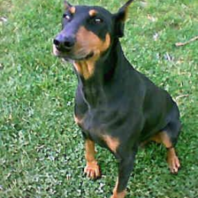
\includegraphics[width=0.25\textwidth, height=0.25\textwidth]{figure/saliency_example/input.png}};
    \node[SIR, label={[align=center]\textbf{Saliency map}}] (id2) [right=of id1] {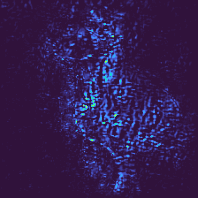
\includegraphics[width=0.25\textwidth, height=0.25\textwidth]{figure/saliency_example/saliency.png}};


    \begin{scope}[shift={($(id2.east)+(0.1cm,0.25\textwidth / 2)$)}]
        \pgfplotscolorbardrawstandalone[
        colormap name=turbo,
        point meta min=0,
        point meta max=1,
        colorbar style={
            height=0.25\textwidth, % Match the height of the images
            width=0.4cm, % Desired width of the colorbar
            ytick={0, 0.5, 1},
            % yticklabels={Low, Medium, High},
        }]
    \end{scope}

    \end{tikzpicture}

    \end{center}
    \caption[Saliency Example]{Figure showing an input image and the corresponding saliency map, generated by an \ac{xai} algorithm which shows the important pixels for the predicted class (Rhodesian Ridgeback). The colorbar and heatmap show the relative saliency for all pixels, with 0 being the least important pixel and 1 being the most important pixel}
    \label{fig:saliency_ex}
\end{figure}

Secondly, many methods which are designed for data tabular data (which have may have 10-20 features) are far too slow when the number of features may be over a hundred thousand. Methods such as \ac{lime}, Occlusion, or Shapley fall into this category, as they permute the input at a rate which scales with the number of inputs.

A solution to this is to segment the image into larger regions, which are treated as one. As opposed to asking "how does the prediction change if we change this pixel", we instead ask "how does the prediction change if we change this {\it region}". All pixels in a region are then awarded the same amount of importance. This drastically reduces the dimensionality of the problem, and allows us to use a much larger range of methods. The output of such methods is thus also a saliency map, but one where each pixel is not given an individual saliency score, but rather a score derived from the larger region in which it is contained.

Regions of pixels can be created in different ways. The simplest option is consider a window of a specific height and width, and slide this window over the image with a specific stride. By adjusting the stride and size, the number of dimensions can be adjusted. The benefit of such a simple approach is that the segmentation itself introduces no extra computation. However, a substantial downside is that each region can contain completely unrelated objects, because the regions are created without considering the underlying image. For example, if a 60 by 60 pixel region contains in its lower right corner a part of a dog, occluding this region could lead to a large change in confidence and thus high importance. However, it is not just the lower right corner that is awarded high importance, but the entire region, which may contain other objects or parts of the background which are not actually important.

By using more sophisticated segmentation methods, we can avoid this problem. Methods such as \ac{slic} \cite{slic} create regions which can be considered more intuitive than simply using a rectangular sliding window. \ac{slic} performs an iterative clustering of pixels, grouping similar pixels into larger regions called superpixels. The downside to this method is that the iterative, CPU-bound process introduces a considerable computational overhead. Figure \ref{fig:segmentationcomp} shows a comparison between the saliency map of the \ac{lime} algorithm applied to an image segmented using rectangular regions and to an image segmented using \ac{slic}. As we can see, the rectangular segmentation means that the some of the grass in the background is given a high saliency, because it happens to be in the same region as the dog's head. Using \ac{slic}, there are few regions which contain both grass and the dog, and thus the high saliency of the dog's face does not affect other parts of the image.

\begin{figure}[H]
    \begin{center}

    \begin{tikzpicture}[
    SIR/.style={rectangle, draw=black!80, thick, minimum size=5mm},
    ]

    \node[SIR, label={[align=center]\textbf{Input image}}] (id1) {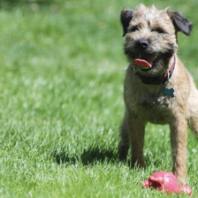
\includegraphics[width=0.25\textwidth, height=0.25\textwidth]{figure/segmentation_comparison/lime_rectangular-img0.png}};
    \node[SIR, label={[align=center]\textbf{\ac{lime} applied to}\\\textbf{rectangular regions}}] (id2) [right=of id1] {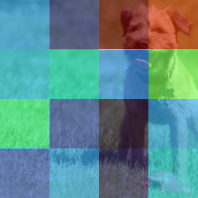
\includegraphics[width=0.25\textwidth, height=0.25\textwidth]{figure/segmentation_comparison/lime_rectangular-img1.png}};
    \node[SIR, label={[align=center]\textbf{\ac{lime} applied to}\\\textbf{superpixel regions}}] (id3) [right=of id2] {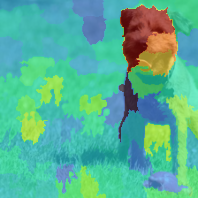
\includegraphics[width=0.25\textwidth, height=0.25\textwidth]{figure/segmentation_comparison/lime_slic-img1.png}};

    \begin{scope}[shift={($(id3.east)+(0.1cm,0.25\textwidth / 2)$)}]
        \pgfplotscolorbardrawstandalone[
        colormap name=turbo,
        point meta min=0,
        point meta max=1,
        colorbar style={
            height=0.25\textwidth, % Match the height of the images
            width=0.4cm, % Desired width of the colorbar
            ytick={0, 0.5, 1},
            % yticklabels={Low, Medium, High},
        }]
    \end{scope}


    \end{tikzpicture}

    \end{center}
    \caption[Segmentation comparison]{Figure showing a comparison between generating saliency maps using the \ac{lime} algorithm on rectangular and superpixel regions. The colorbar and heatmap show the relative saliency for all regions, with 0 being the least important region and 1 being the most important region}
    \label{fig:segmentationcomp}
\end{figure}



\subsection{Specific methods} \label{section:xaimethodsbackground}


The following section goes through several specific \ac{xai} methods. This serves two purposes: Firstly, by explaining how commonly used \ac{xai} methods function in more detail, it is easier to understand how \ac{xai} methods work in practice. Secondly, this section also covers the specific methods that will be integrated into the three \ac{ood} detection frameworks. By thoroughly detailing the functions of these methods in this chapter, it becomes easier to analyse and explain the proposed methods in chapter \ref{chapter:methodology} and the results in chapter \ref{chapter:experiments}.
\\


\subsubsection{Local Interpretable Model-Agnostic Explanations (LIME)}

\ac{lime} \cite{lime} is a post-hoc, model independent \ac{xai} method. The method is built on the idea that while the decision function of a large neural network (or any other large model) might be far too complex to easily interpret, it can most likely be approximated quite well by a simpler function, as long as we only look at the feature space around a single data point. For example, we could approximate a large feed forward neural network with a simple linear regression model, which can be intrinsically explained due to its low complexity.

To create a locally interpretable model, we need a neighbourhood of data points around our point of interest. To do this, we can sample a number of points from our dataset and weigh them by their distance to our original point. This sampling can be done in many ways, for example by calculating a mean and variance for each feature and sampling from a normal distribution. For image data, we can create new points similar to the image by masking out different regions of the image \cite{molnar}. The distance measure depends on the type of data we are dealing with. Regardless, the distance values are passed through a smoothing kernel which can be tuned to adjust the size of the "neighbourhood".

With these new data points, we can generate new predictions using the original, complex model. Thus, we now have a series of points, each with a weighting based on their distance to our original point, and each with a predicted score from our original model. With such a dataset, we can train a simpler model, which will then approximate the complex model around the point of interest. By inspecting this simple model (for example: the learned weights of a linear regression model, or the structure of a decision tree), we can learn approximately how the complex model functions in a region around this single data point.

\subsubsection{Occlusion methods}

Occlusion methods are a family of post-hoc, model independent \ac{xai} methods. They function by masking different parts of the image and inspecting the change in output score. If an area leads to a large drop in softmax score for the predicted class when masked, this area must have been important for the network when making the prediction. The mask can be as simple as replacing all masked pixels with a single color, such as gray \cite{occlusion}, or they could use more advanced inpainting methods using generative models, for example by replacing a masked tumor with generated healthy tissue. 

Regardless of the mask, one can easily calculate the importance of any pixel for a prediction by calculating the average change in the output score for all masks which contain the specific pixel \cite{diagnostic}. Occlusion methods have the advantage of being completely model independent, since they do not consider the internals of the model. However, the computation can be expensive, because we need to run a forward pass for each position of the mask on the image. % Figure \ref{fig:occlusion} shows the process visually.

\subsubsection{Class Activation Mapping (CAM)}

\ac{cam} \cite{cam} is a model dependent, post hoc \ac{xai} method, which is used on Convolutional Neural Nets (\ac{cnn}s). For a specific output node of a model (for example, the one denoting the presence of a specific class, such as "cat"), \ac{cam} outputs a heat map showing which areas of the input image contributed to this node. In this way, \ac{cam} gives a visual explanation to which parts of an image the model focused on when making a decision to classify an image to a specific class. This method is model dependent, because it requires a specific architecture in the final layers of the network to work.

\ac{cam} is a relatively simple method to understand. It exploits the fact that various convolutional layers of \ac{cnn}s actually behave as object detectors, even when the training objective is classification \cite{cam}. As \cite{lenet5} explains, the earlier layers "extract elementary visual features such as oriented edges, end-points [or] corners", which can be used by subsequent layers to detect higher-order features. In this manner, the final convolutional layer will detect very high level visual features, combining the extracted information from all the previous layers. This layer is composed of several feature maps, where each map can be thought of as denoting the presence of some specific feature across the original image. The authors perform global average pooling (GAP) on these feature maps, giving a single value for each map, which is followed by a single dense layer and the Softmax activation function. In this way, each output node in the final layer is a weighted sum of all the global average pooled feature maps from the final convolutional layer. This means that we can represent the areas of the image which were used to perform the classification by performing the same weighted sum on the actual feature maps instead, which gives us a heat map which we can overlay on the original image (after upsampling the feature maps).

Figure \ref{camimg} shows the process visually. From this we can see that the resulting Class Activation Map (bottom right) gives an intuitive explanation for why the image in the top left gives a high score for the presence of the class "Australian Terrier".

\begin{figure}[h]
\centerline{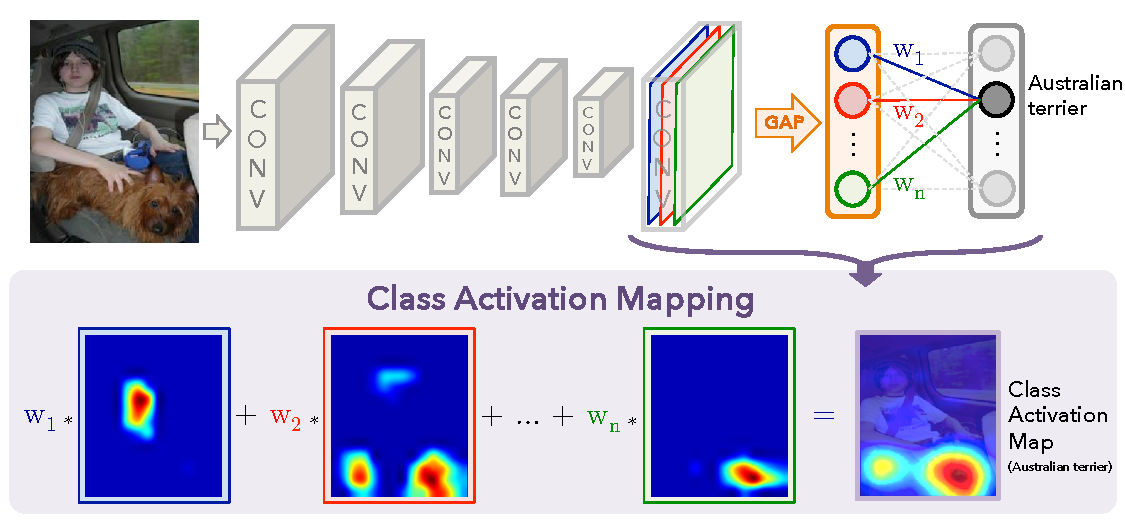
\includegraphics[width=3.25in]{figure/cam.pdf}}
\caption{Figure taken from \cite{cam}, showing the steps required to create a Class Activation Map}
\label{camimg}
\end{figure}

\begin{figure}[H]
    \begin{center}
    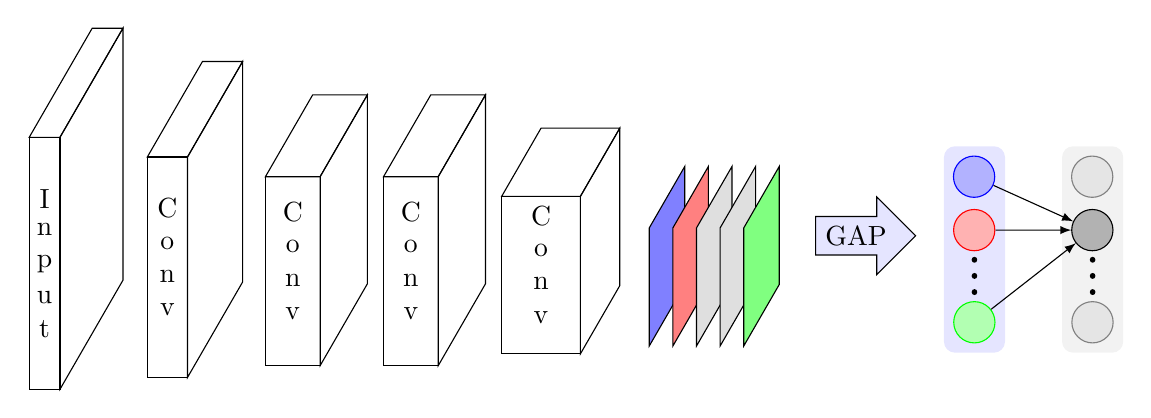
\begin{tikzpicture}[x={(1,0)},y={(0,1)},z={({cos(60)},{sin(60)})}, scale=1.5]
%
% comment these out if you want to see where the axes point to
% \draw[-latex] (0,0,0) -- (3,0,0) node[below]{$x$};
% \draw[-latex] (0,0,0) -- (0,3,0) node[left]{$y$};
% \draw[-latex] (0,0,0) -- (0,0,3) node[below]{$z$};
% a plane
\draw pic (box1-1) at (1,-1.6/2,0) {fake box=white!70!gray with dimensions {1/1.6/1.6} and {2*1.6} and {1*1.6} and Input};

\foreach \X [count=\Y] in {1.4,1.2,1.2,1}
{
    \draw pic (box1-\Y) at (\Y+1,-\X/2,0) {fake box=white!70!gray with dimensions {1/\X/\X} and {2*\X} and {1*\X} and Conv};
}

\foreach \X/\Col in {6.5/blue,6.7/red,6.9/lightgray, 7.1/lightgray, 7.3/green}
{\draw[canvas is yz plane at x = \X, transform shape, fill =
\Col!50!white] (0,0.10) rectangle (1,-0.5);}
% \draw[gray!60,thick] (6.3,-0.1,-1.6) coordinate (1-1) -- (6.3,-0.1,0.6) coordinate (1-2) -- (6.3,2.,0.6) coordinate (1-3) -- (6.3,2.1,-1.6) coordinate (1-4) -- cycle;
% \draw[gray!60,thick] (7.1,-0.1,-1.6) coordinate (2-1) -- (7.1,-0.1,0.6) coordinate (2-2) -- (7.1,2.,0.6) coordinate (2-3) -- (7.1,2.1,-1.6) coordinate (2-4) -- cycle;
% \foreach \X in {4,1,3}
% {\draw[gray!60,thick] (1-\X) -- (2-\X);}
%
\node[draw,single arrow, fill=blue!10] at (8,0.5,0) {GAP};
\node[circle,draw,blue,fill=blue!30] (A1) at (9,1,0) {~~~};
\node[circle,draw,red,fill=red!30,below=4pt of A1] (A2) {~~~};
\node[circle,draw,green,fill=green!30,below=18pt of A2] (A3) {~~~};
\draw[circle dotted, line width=2pt,shorten <=3pt] (A2) -- (A3);
\node[circle,draw,gray,fill=gray!20] (B1) at (10,1,0) {~~~};
\node[circle,draw,fill=gray!60,below=4pt of B1] (B2) {~~~};
\node[circle,draw,gray,fill=gray!20,below=18pt of B2] (B3) {~~~};
\draw[circle dotted, line width=2pt,shorten <=3pt] (B2) -- (B3);
\begin{scope}[on background layer]
\node[orange,thick,rounded corners,fill=blue!10,fit=(A1) (A3)]{};
\node[gray,thick,rounded corners,fill=gray!10,fit=(B1) (B3)]{};
\end{scope}
\foreach \X in {1,2,3}
{\draw[-latex] (A\X) -- (B2);}
\end{tikzpicture}

    \end{center}
    \caption[CNN example]{Figure showing a high level overview of how a CNN functions}
    \label{fig:cam2}
\end{figure}

Although \ac{cam} is an intuitive and effective method of visualizing the inner workings of a \ac{cnn}, it has some downsides. Firstly, it is highly model dependent, requiring that the model only have a single dense layer after the convolutions. Although there are some \ac{sota} models which only use a single dense layer, this still places a limit on what models can be used, or requires the simplification of models that use more than a single dense layer. \cite[4]{cam} notes a 1-2\% drop in classification performance when performing this simplification. Secondly, the output of \ac{cam} is simply a weighted sum of all the feature maps after the final convolutional layer. As we move deeper in a \ac{cnn}, we reduce the spatial resolution by downsampling, while increasing the number of channels (increasing the depth of the output while reducing the height and width). Because of this, the \ac{cam} will have a drastically lower resolution than the original image, often less than $10 \times 10$, while the input image may be hundreds of pixels in both dimensions. Because of this, \ac{cam} can only show general areas, as opposed to pixel wise explanations.
\\

\subsubsection{Gradient Class Activation Mapping (GradCAM)} \label{section:gradcam}

\ac{gradcam} \cite{gradcam} is an improvement on \ac{cam}, which generalizes the method to function with any \ac{cnn} architecture, thus making the method much less model dependent and avoiding the performance drop incurred when simplifying the model with \ac{cam}. Instead of using the weights of a final layer to calculate a weighted sum of feature maps in the last convolutional layer, \ac{gradcam} uses gradients flowing from the relevant output node to the activation maps to calculate the weights for each feature map. Furthermore, the authors prove that this method is a strict generalization of \ac{cam} \cite[5]{gradcam}, so that no information is lost by using gradients instead of weights.

Like the simplicity of the \ac{cam} method, the calculation of the weights using the gradients is also quite simple, as seen in Equation \ref{gradcameq}.

\begin{equation}
\alpha^c_k = \frac{1}{Z} \sum_i \sum_j \frac{\delta y^c}{\delta A^k_{ij}}
\label{gradcameq}
\end{equation}

Here, $c$ represents the index of the class we are interested in, $k$ the index of the feature map, and $i$ and $j$ the width and height of the image. $y^c$ is the element of the output vector $y$ which corresponds to the class $c$, while $A^k$ is the $k$'th feature map. $Z$ is equal to the number of elements in each channel of the feature map, and simply normalizes the sum. Thus, we are actually just performing global average pooling of the gradients of $A^k$ with respect to $y^c$, which gives us a single value we can use as the weight for this feature map. Doing this for all feature maps for a specific class gives us all the weights we need to calculate a weighted sum, which we can upsample and visualize to get an explanation for the decision of the \ac{cnn}.

Thus, \ac{gradcam} improves upon \ac{cam} by making the method less model dependent. However, the explanations are still the same low resolution, which may not be ideal in all cases.
\\

\subsubsection{Guided Backpropagation} \label{section:guidebackpropagation}

\ac{gbp} \cite{gbp} is another \ac{xai} method which utilizes the gradients of the network to calculate saliencies. In this case, we do not stop at the final feature map, but backpropagate through the entire network to the input image. Simply backpropagating in this way produces a saliency map for the entire input image. However, \cite{gbp} finds that by only backpropagating positive gradients through \acs{relu} functions, they are able to produce "sharper visualizations of descriptive image regions than the previously known methods". Although the choice to simply neglect negative gradients when backpropagating lacks theoretical justification, \ac{gbp} has been shown to be accurate and trustworthy compared to other methods \cite{arras2022clevr, pianpanit2021parkinson}. Compared to the previous methods, \ac{gbp} differs in the sense that it produces a saliency value for every single input feature (every pixel, for example) as opposed to regions.

\subsubsection{Integrated Gradients} \label{section:integratedgradients}

Integrated Gradients \cite{integratedgradients} is another gradient based \ac{xai} method. The method was developed as part of an effort to create an \ac{xai} method which satisfies two axioms; sensitivity, and implementation invariance. Sensitivity states that if an input and a baseline differ in only one input feature, and have different outputs, then this input feature should have non-zero saliency. \cite{integratedgradients} shows that gradients violate this property because "the prediction function may flatten at the input and thus have zero gradient despite the function value at the input being different from that at the baseline". Implementation invariance states that if two models are functionally identical (their outputs are equal for all inputs), then their attributions should be identical as well. Gradients satisfy this property, but methods which modify the gradients, such as \ac{gbp} and \ac{lrp} \cite{lrp}, break this axiom.

Both these axioms represent desirable qualities for an \ac{xai} method; we don't want our attribution method to miss any features which lead to a change in the model prediction, and we don't want the internal structure of the model to affect the attribution if it does not affect the output score in any way. Thus, it is problematic that there are few methods which satisfy both criteria. \cite{integratedgradients} finds that by integrating the gradients of the network in the straight line path between a baseline and the input, both these axioms are satisfied. Mathematically, the saliency for a specific input feature $\mathbf{x}_i$ is defined as follows, given an input $\mathbf{x}$, a baseline $\mathbf{x'}$ and a deep learning model $f$:

\begin{equation}
    \text{IntegratedGradients}_i(\mathbf{x}) := (\mathbf{x}_i - \mathbf{x}_i') \times \int_{\alpha = 0}^1 \frac{\delta f(\mathbf{x}' + \alpha \times (\mathbf{x} - \mathbf{x}'))}{\delta \mathbf{x}_i}d\alpha
\end{equation}

By cumulating the gradients of the network at all points between the baseline and the input, \cite{integratedgradients} manages to combine the implementation invariance of gradients with the sensitivity of techniques like \ac{lrp}. In addition, they prove that if the model $f$ is differentiable "almost everywhere", then the sum of all attributions is equal to the difference in output between the baseline and the input:

\begin{equation}
    \sum_{i=1}^n \text{IntegratedGradients}_i(\mathbf{x}) = f(\mathbf{x}) - f(\mathbf{x'})
\end{equation}

If we then choose a baseline which has $f(\mathbf{x'}) \approx 0$, we see that integrated gradients is equivalent to distributing the output prediction amongst the input features, a very desirable interpretation for an \ac{xai} attribution method.


\section{Out-of-Distribution Detection} \label{ood_intro}

This section discusses \ac{ood} detection, the field which attempts to tackle the second problem discussed in the introduction and which is the main focus of this thesis; that \ac{ml} models have significantly worse performance on \ac{ood} data points and will often "fail silently", making completely wrong predictions with apparent high confidence \cite{adversarial}. \ac{ood} detection is a developing field, and still in an initial stage \cite{ooddl}. In 2017, \cite{oodbaseline} proposed a baseline \ac{ood} detection method. This section will discuss this method and the methods which follow it.

\subsection{Motivation for Out-of-Distribution Detection}

When training a model using supervised learning, we implicitly use the "closed-world assumption", which means that we assume that test data will be drawn from the same distribution as the training data \cite{oodoverview}. However, when a model is deployed, the data we see may not obey this assumption. Without \ac{ood} detection, the model will behave in the exact same way when encountering \ac{ood} samples or in distribution (\ac{id}) samples, and may even claim to be highly confident in its prediction although the sample is far away from the distribution of the training data \cite[1]{energy}. In any system where models make high impact decisions, this is a huge problem. We do not want a medical \ac{ai} system to attempt to classify a rare disease that was not part of the training data, nor do we want an autonomous car to continue to drive on snowy dirt roads if its training data only contains the sunny streets of San Francisco. Thus, \ac{ood} detection methods are necessary, so that \ac{ood} samples can be caught before the model takes any (potentially catastrophic) action.

Intuitively, one might assume that distinguishing \ac{id} and \ac{ood} samples from each other can be solved by simple binary classification using a dataset of \ac{id} samples and one of \ac{ood} samples. Indeed, if one has sufficient amount of high quality \ac{ood} samples, this can be done. However, this can be difficult to obtain in practice \cite[15]{oodoverview}. A key problem is that \ac{ood} data is, almost by definition, data which we do not have at development and training time of a specific model. \ac{ood} data is unexpected and surprising data, which cannot be predicted before hand; we cannot possibly predict all situations a self-driving car could end up in, nor account for every single disease in the world when developing a medicinal \ac{ai} system. Thus, we require more sophisticated methods of \ac{ood} detection, which catch \ac{ood} data points in a general manner and do not rely on explicit examples of \ac{ood} data. Indeed, the majority of methods developed in the field of \ac{ood} detection do not rely on such auxiliary datasets \cite{openood}. % TODO check this citation

\subsection{Semantic versus covariate shift}

The first distinction to make in \ac{ood} detection tasks is whether an \ac{ood} sample is \ac{ood} because of {\it semantic} or {\it covariate} shift. Semantic shift refers to samples with different classes than the ones the model is trained on. A picture of a giraffe would represent a semantic shift for a model trained to differentiate between different breeds of dogs, as a giraffe does not belong to any breed of dog. Covariate shift refers to samples which come from a different distribution while still belonging to one of the classes of the original data set. An image of a Beagle puppy could represent covariate shift for a dog breed classifier despite Beagle being one of the classes, if all \ac{id} images were of adult dogs. Likewise, an image of a dog in a dark room could represent covariate shift, if all the \ac{id} images were of dogs outside, in well lit conditions. Figure \ref{fig:semanticcovariate} shows this distinction visually. Here, we can easily see the difference between covariate and semantic shift; covariate shifted images come from the same classes as \ac{id} samples, while semantically shifted images come from completely unknown classes.

\begin{figure}[H]
    \begin{center}

    \begin{tikzpicture}[
    SIR/.style={rectangle, draw=black!80, thick, minimum size=5mm},
    ]

    \node[SIR, label={[align=center, above=0.2cm]\textbf{In Distribution}\\\textbf{images}}] (id1) {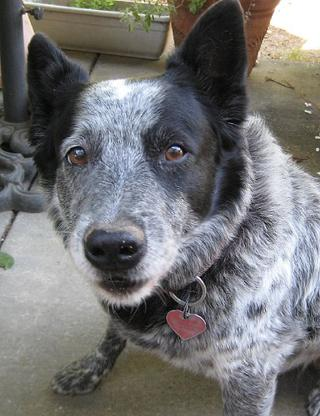
\includegraphics[width=0.25\textwidth, height=0.25\textwidth]{figure/semanticcovariate/id1.jpg}};
    \node[SIR] (id2) [below=of id1] {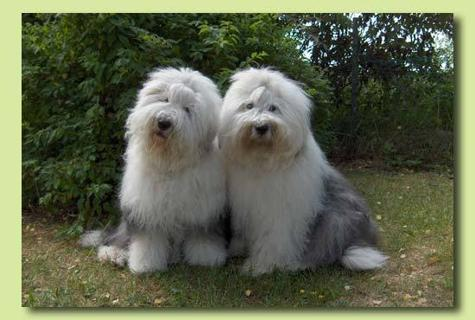
\includegraphics[width=0.25\textwidth, height=0.25\textwidth]{figure/semanticcovariate/id2.jpg}};
    \node[SIR] (id3) [below=of id2] {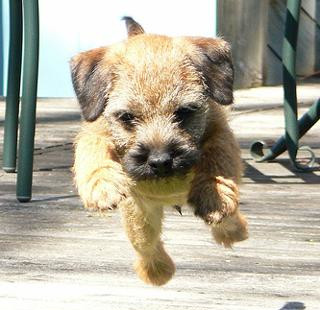
\includegraphics[width=0.25\textwidth, height=0.25\textwidth]{figure/semanticcovariate/id3.jpg}};

    \node[SIR, label={[align=center, above=0.2cm]\textbf{Covariate shifted}\\\textbf{images}}, right=of id1] (cov1) {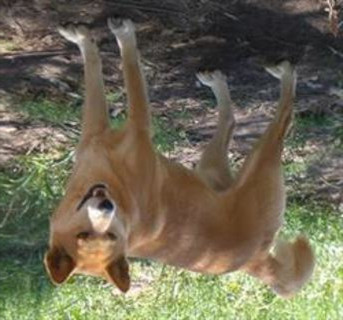
\includegraphics[width=0.25\textwidth, height=0.25\textwidth]{figure/semanticcovariate/cov1.jpg}};
    \node[SIR] (cov2) [below=of cov1] {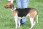
\includegraphics[width=0.25\textwidth, height=0.25\textwidth]{figure/semanticcovariate/cov2.jpg}};
    \node[SIR] (cov3) [below=of cov2] {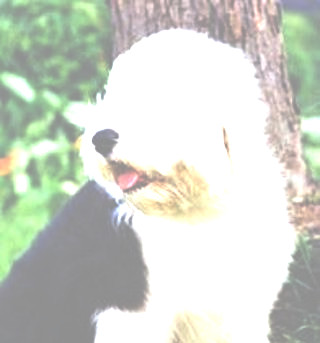
\includegraphics[width=0.25\textwidth, height=0.25\textwidth]{figure/semanticcovariate/cov3.jpg}};

    \node[SIR, label={[align=center, above=0.2cm]\textbf{Semantically shifted}\\\textbf{images}}, right=of cov1] (sem1) {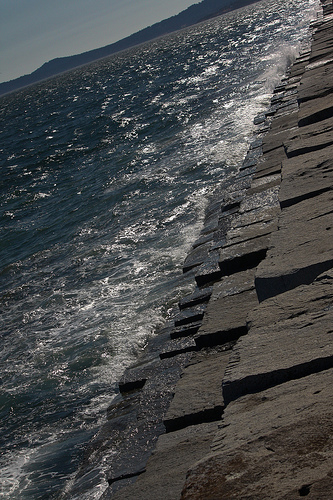
\includegraphics[width=0.25\textwidth, height=0.25\textwidth]{figure/semanticcovariate/sem1.jpg}};
    \node[SIR] (sem2) [below=of sem1] {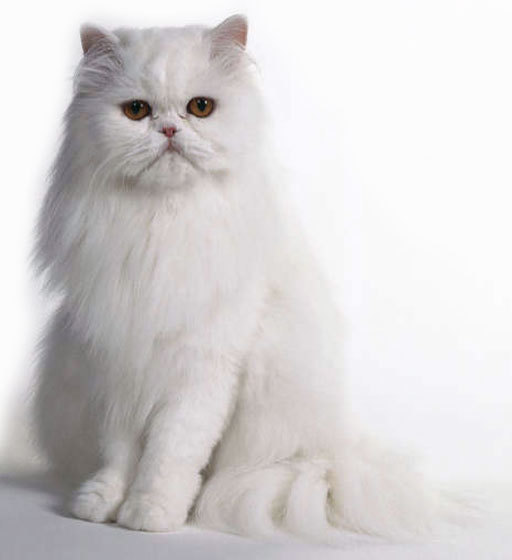
\includegraphics[width=0.25\textwidth, height=0.25\textwidth]{figure/semanticcovariate/sem2.jpg}};
    \node[SIR] (sem3) [below=of sem2] {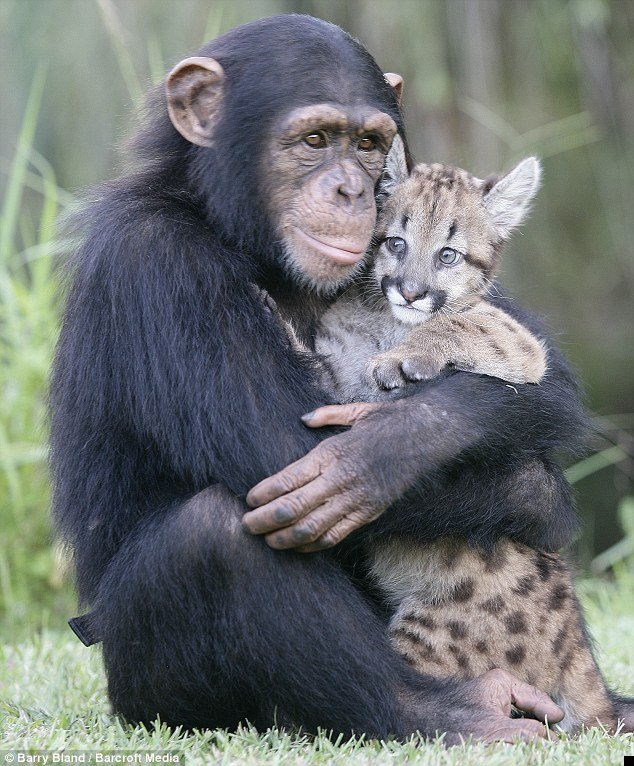
\includegraphics[width=0.25\textwidth, height=0.25\textwidth]{figure/semanticcovariate/sem3.jpg}};

    \begin{scope}[on background layer={color=id!50}]
        \fill (-2.5,2.15) rectangle (2.5,-12.1);
    \end{scope}

    \begin{scope}[on background layer={color=near!50}]
        \fill (2.5,2.15) rectangle (7.5,-12.1);
    \end{scope}

    \begin{scope}[on background layer={color=far!50}]
        \fill (7.5,2.15) rectangle (12.5,-12.1);
    \end{scope}

    \end{tikzpicture}

    \caption[Mean Saliency visual explanation]{Figure showing in-distribution, covariate shifted and semantically shifted images for an imagined dog breed classifier. Images are taken from the ImageNet dataset}
    \label{fig:semanticcovariate}

    \end{center}
\end{figure}

The detection of semantic shift, as opposed to covariate shift, is the main focus of most \ac{ood} detection tasks \cite{oodoverview}. In many applications, it is expected that the model should be able to generalize its prediction to covariate-shifted data, and therefore the focus is on detecting semantic shift. However, the field of medical image classification is one where detecting covariate shift is also important, as the model should only make predictions on data points which are very similar to its training data \cite{oodoverview}.

Given that the detection of semantic shift has been the main focus of most \ac{ood} literature, my work will primarily deal with semantic shift as well. Thus, unless otherwise specified, when I refer to \ac{ood} data points, I mean data points which are semantically shifted, i.e that come from another class than those the model has been trained on.

\subsection{Benchmarking}

The performance of an \ac{xai} is hard to quantify, because the quality of an explanation is not easily reduced to a number. For \ac{ood} detection, performance is much easier to measure, as the problem can be described as a binary classification problem, with \ac{ood} and \ac{id} samples as the positive and negative class, respectively. Thus, we can calculate many different metrics and compare methods against each other. For \ac{ood} methods, the two most common metrics to report are \ac{fpr95} and the \ac{auroc} (see section \ref{section:aurocfpr95}). It is common to use ImageNet or CIFAR as the \ac{id} dataset, and calculate \ac{fpr95} and \ac{auroc} on other datasets which contain no overlapping class labels. When selecting \ac{ood} datasets, it is common to differentiate between \textbf{Near-\ac{ood}} and \textbf{Far-\ac{ood}}. Far-\ac{ood} samples are samples which are drastically different from the \ac{id} samples, while Near-\ac{ood} samples only differ slightly. For a cat-versus-dog classifier, a tiger and a wolf would represent Near-\ac{ood} semantic shift, while a plane and a car would represent Far-\ac{ood} semantic shift. As one might expect, detecting Near-\ac{ood} samples is much harder than Far-\ac{ood}.

% FPR95 is, as the name implies, the number of false positives (i.e the number of ID data points that the method falsely believes to be \ac{ood}) when 95\% of the \ac{ood} data points are correctly detected. AUROC can defined as the chance that a random ID data point has a higher ID-score than a random \ac{ood} data point \cite{openood}. An AUROC of 0.5 is equivalent to random guessing, while an AUROC of 1 is a perfect model that catches all \ac{ood} data points.


In 2021, \cite{oodoverview} defined a generalized \ac{ood} detection framework, and in 2023 \cite{openood} introduced a comprehensive benchmark called OpenOOD, which evaluates all relevant \ac{ood} methods under this framework. Prior to this work, different methods were tested on different benchmarks, with different image preprocessing procedures, and with other externalities which inhibited effective comparison between methods \cite{openood}.

OpenOOD includes 11 different benchmarks across Anomaly Detection, Open Set Recognition and \ac{ood} detection, three fields which are very closely related. Of these, 4 benchmarks are used to test methods for standard \ac{ood} detection, which are the ones I will be concerned with. Each benchmark is defined by an \ac{id} dataset, with 6 or more corresponding \ac{ood} datasets, separated into Near-\ac{ood} and Far-\ac{ood}. For each benchmark, \ac{auroc}, \ac{aupr} and \ac{fpr95} is reported over all \ac{ood} datasets, and Near-\ac{ood} \ac{auroc} is used to rank methods against each other.

\subsection{Methods}

This section will follow the same outline as section \ref{chapter:xai}; firstly, the overarching categories of methods will be discussed, followed by a more detailed look at a selection of specific methods within the field.
\\

The field of \ac{ood} is separated into four categories of methods \cite{oodoverview}:

\begin{itemize}
  \item Classification-based methods
  \item Density-based methods
  \item Distance-based methods
  \item Reconstruction-based methods
\end{itemize}

All methods can also be categorized by whether they are post-hoc or training based. Post-hoc methods take an already trained network and attempt to extract information which separates \ac{id} and \ac{ood} samples out of the network during inference. These methods have the obvious advantage that they can work out of the box with large pre-trained network without requiring expensive training from scratch. Training based methods train the network in ways which maximize the difference between \ac{id} and \ac{ood} samples. These methods do not necessarily require \ac{ood} samples, but can train using auxiliary loss functions which amplify the differences in network behaviour when faced with \ac{ood} data as opposed to \ac{id}. Regardless, these methods come with a much higher computational requirement than post-hoc methods, as they require training from scratch or at least retraining using the new loss criterion. 

Given the fact that post-hoc methods can be applied to trained networks out of the box, it is quite common to combine both post-hoc and training strategies to achieve the best performance.


Below follows a short explanation of each the four categories mentioned above.
\\

\subsubsection{Classification-based methods}

Classification-based methods usually use the softmax score or logits of a model to attempt to distinguish \ac{ood} and \ac{id} samples. \cite{oodbaseline} made the observation that while the softmax score may be a poor indication of the actual confidence of the model on a single data point, it is still higher on average for \ac{id} samples as opposed to \ac{ood} samples. By using this simple distinction, they created a baseline model which separated \ac{ood} and \ac{id} samples. Using input perturbations and temperature scaling, \cite{odin} further improved on this method, by amplifying the difference in softmax score of \ac{id} and \ac{ood} data. 

More generally, classification-based methods do not need to use the softmax score, but may attempt to find any metric which separates the distribution of \ac{id} samples from \ac{ood} samples. Figure \ref{fig:ood_metric} shows the probability density for an unspecified metric for both \ac{ood} and \ac{id} samples. The goal of classification-based \ac{ood} detection is to find metrics or training methods which make these probability densities have as little overlap as possible, such that they are easily separated by a threshold. The threshold, often denoted as $\delta$, is a parameter that needs to be set at a specific value based on the values of a validation \ac{id} and validation \ac{ood} data set. Often, one sets the $\delta$ such that a certain percentage of \ac{ood} samples in the validation set are correctly detected, for example 95\%.

There are several \ac{sota} methods which utilize a classification-based approach, and these make up a large part of the representative methodologies for \ac{ood} detection today \cite[8]{oodoverview}. As such, I shall devote the majority of section \ref{ood_specific} to classification-based methods.

\begin{figure}
    \label{fig:ood_metric}
    \begin{center}
        %% Creator: Matplotlib, PGF backend
%%
%% To include the figure in your LaTeX document, write
%%   \input{<filename>.pgf}
%%
%% Make sure the required packages are loaded in your preamble
%%   \usepackage{pgf}
%%
%% Also ensure that all the required font packages are loaded; for instance,
%% the lmodern package is sometimes necessary when using math font.
%%   \usepackage{lmodern}
%%
%% Figures using additional raster images can only be included by \input if
%% they are in the same directory as the main LaTeX file. For loading figures
%% from other directories you can use the `import` package
%%   \usepackage{import}
%%
%% and then include the figures with
%%   \import{<path to file>}{<filename>.pgf}
%%
%% Matplotlib used the following preamble
%%   \def\mathdefault#1{#1}
%%   \everymath=\expandafter{\the\everymath\displaystyle}
%%   \IfFileExists{scrextend.sty}{
%%     \usepackage[fontsize=10.000000pt]{scrextend}
%%   }{
%%     \renewcommand{\normalsize}{\fontsize{10.000000}{12.000000}\selectfont}
%%     \normalsize
%%   }
%%   
%%   \makeatletter\@ifpackageloaded{underscore}{}{\usepackage[strings]{underscore}}\makeatother
%%
\begingroup%
\makeatletter%
\begin{pgfpicture}%
\pgfpathrectangle{\pgfpointorigin}{\pgfqpoint{6.400000in}{4.800000in}}%
\pgfusepath{use as bounding box, clip}%
\begin{pgfscope}%
\pgfsetbuttcap%
\pgfsetmiterjoin%
\definecolor{currentfill}{rgb}{1.000000,1.000000,1.000000}%
\pgfsetfillcolor{currentfill}%
\pgfsetlinewidth{0.000000pt}%
\definecolor{currentstroke}{rgb}{1.000000,1.000000,1.000000}%
\pgfsetstrokecolor{currentstroke}%
\pgfsetdash{}{0pt}%
\pgfpathmoveto{\pgfqpoint{0.000000in}{0.000000in}}%
\pgfpathlineto{\pgfqpoint{6.400000in}{0.000000in}}%
\pgfpathlineto{\pgfqpoint{6.400000in}{4.800000in}}%
\pgfpathlineto{\pgfqpoint{0.000000in}{4.800000in}}%
\pgfpathlineto{\pgfqpoint{0.000000in}{0.000000in}}%
\pgfpathclose%
\pgfusepath{fill}%
\end{pgfscope}%
\begin{pgfscope}%
\pgfsetbuttcap%
\pgfsetmiterjoin%
\definecolor{currentfill}{rgb}{1.000000,1.000000,1.000000}%
\pgfsetfillcolor{currentfill}%
\pgfsetlinewidth{0.000000pt}%
\definecolor{currentstroke}{rgb}{0.000000,0.000000,0.000000}%
\pgfsetstrokecolor{currentstroke}%
\pgfsetstrokeopacity{0.000000}%
\pgfsetdash{}{0pt}%
\pgfpathmoveto{\pgfqpoint{0.800000in}{0.528000in}}%
\pgfpathlineto{\pgfqpoint{5.760000in}{0.528000in}}%
\pgfpathlineto{\pgfqpoint{5.760000in}{4.224000in}}%
\pgfpathlineto{\pgfqpoint{0.800000in}{4.224000in}}%
\pgfpathlineto{\pgfqpoint{0.800000in}{0.528000in}}%
\pgfpathclose%
\pgfusepath{fill}%
\end{pgfscope}%
\begin{pgfscope}%
\pgfpathrectangle{\pgfqpoint{0.800000in}{0.528000in}}{\pgfqpoint{4.960000in}{3.696000in}}%
\pgfusepath{clip}%
\pgfsetbuttcap%
\pgfsetroundjoin%
\definecolor{currentfill}{rgb}{0.501961,0.501961,0.501961}%
\pgfsetfillcolor{currentfill}%
\pgfsetfillopacity{0.500000}%
\pgfsetlinewidth{1.003750pt}%
\definecolor{currentstroke}{rgb}{0.501961,0.501961,0.501961}%
\pgfsetstrokecolor{currentstroke}%
\pgfsetstrokeopacity{0.500000}%
\pgfsetdash{}{0pt}%
\pgfsys@defobject{currentmarker}{\pgfqpoint{1.025455in}{0.696000in}}{\pgfqpoint{5.534545in}{1.722527in}}{%
\pgfpathmoveto{\pgfqpoint{1.025455in}{0.696000in}}%
\pgfpathlineto{\pgfqpoint{1.025455in}{0.696000in}}%
\pgfpathlineto{\pgfqpoint{1.029968in}{0.696000in}}%
\pgfpathlineto{\pgfqpoint{1.034482in}{0.696000in}}%
\pgfpathlineto{\pgfqpoint{1.038995in}{0.696000in}}%
\pgfpathlineto{\pgfqpoint{1.043509in}{0.696000in}}%
\pgfpathlineto{\pgfqpoint{1.048023in}{0.696000in}}%
\pgfpathlineto{\pgfqpoint{1.052536in}{0.696000in}}%
\pgfpathlineto{\pgfqpoint{1.057050in}{0.696000in}}%
\pgfpathlineto{\pgfqpoint{1.061563in}{0.696000in}}%
\pgfpathlineto{\pgfqpoint{1.066077in}{0.696000in}}%
\pgfpathlineto{\pgfqpoint{1.070591in}{0.696000in}}%
\pgfpathlineto{\pgfqpoint{1.075104in}{0.696000in}}%
\pgfpathlineto{\pgfqpoint{1.079618in}{0.696000in}}%
\pgfpathlineto{\pgfqpoint{1.084131in}{0.696000in}}%
\pgfpathlineto{\pgfqpoint{1.088645in}{0.696000in}}%
\pgfpathlineto{\pgfqpoint{1.093159in}{0.696000in}}%
\pgfpathlineto{\pgfqpoint{1.097672in}{0.696000in}}%
\pgfpathlineto{\pgfqpoint{1.102186in}{0.696000in}}%
\pgfpathlineto{\pgfqpoint{1.106699in}{0.696000in}}%
\pgfpathlineto{\pgfqpoint{1.111213in}{0.696000in}}%
\pgfpathlineto{\pgfqpoint{1.115727in}{0.696000in}}%
\pgfpathlineto{\pgfqpoint{1.120240in}{0.696000in}}%
\pgfpathlineto{\pgfqpoint{1.124754in}{0.696000in}}%
\pgfpathlineto{\pgfqpoint{1.129267in}{0.696000in}}%
\pgfpathlineto{\pgfqpoint{1.133781in}{0.696000in}}%
\pgfpathlineto{\pgfqpoint{1.138295in}{0.696000in}}%
\pgfpathlineto{\pgfqpoint{1.142808in}{0.696000in}}%
\pgfpathlineto{\pgfqpoint{1.147322in}{0.696000in}}%
\pgfpathlineto{\pgfqpoint{1.151835in}{0.696000in}}%
\pgfpathlineto{\pgfqpoint{1.156349in}{0.696000in}}%
\pgfpathlineto{\pgfqpoint{1.160863in}{0.696000in}}%
\pgfpathlineto{\pgfqpoint{1.165376in}{0.696000in}}%
\pgfpathlineto{\pgfqpoint{1.169890in}{0.696000in}}%
\pgfpathlineto{\pgfqpoint{1.174403in}{0.696000in}}%
\pgfpathlineto{\pgfqpoint{1.178917in}{0.696000in}}%
\pgfpathlineto{\pgfqpoint{1.183431in}{0.696000in}}%
\pgfpathlineto{\pgfqpoint{1.187944in}{0.696000in}}%
\pgfpathlineto{\pgfqpoint{1.192458in}{0.696000in}}%
\pgfpathlineto{\pgfqpoint{1.196972in}{0.696000in}}%
\pgfpathlineto{\pgfqpoint{1.201485in}{0.696000in}}%
\pgfpathlineto{\pgfqpoint{1.205999in}{0.696000in}}%
\pgfpathlineto{\pgfqpoint{1.210512in}{0.696000in}}%
\pgfpathlineto{\pgfqpoint{1.215026in}{0.696000in}}%
\pgfpathlineto{\pgfqpoint{1.219540in}{0.696000in}}%
\pgfpathlineto{\pgfqpoint{1.224053in}{0.696000in}}%
\pgfpathlineto{\pgfqpoint{1.228567in}{0.696000in}}%
\pgfpathlineto{\pgfqpoint{1.233080in}{0.696000in}}%
\pgfpathlineto{\pgfqpoint{1.237594in}{0.696000in}}%
\pgfpathlineto{\pgfqpoint{1.242108in}{0.696000in}}%
\pgfpathlineto{\pgfqpoint{1.246621in}{0.696000in}}%
\pgfpathlineto{\pgfqpoint{1.251135in}{0.696000in}}%
\pgfpathlineto{\pgfqpoint{1.255648in}{0.696000in}}%
\pgfpathlineto{\pgfqpoint{1.260162in}{0.696000in}}%
\pgfpathlineto{\pgfqpoint{1.264676in}{0.696000in}}%
\pgfpathlineto{\pgfqpoint{1.269189in}{0.696000in}}%
\pgfpathlineto{\pgfqpoint{1.273703in}{0.696000in}}%
\pgfpathlineto{\pgfqpoint{1.278216in}{0.696000in}}%
\pgfpathlineto{\pgfqpoint{1.282730in}{0.696000in}}%
\pgfpathlineto{\pgfqpoint{1.287244in}{0.696000in}}%
\pgfpathlineto{\pgfqpoint{1.291757in}{0.696000in}}%
\pgfpathlineto{\pgfqpoint{1.296271in}{0.696000in}}%
\pgfpathlineto{\pgfqpoint{1.300784in}{0.696000in}}%
\pgfpathlineto{\pgfqpoint{1.305298in}{0.696000in}}%
\pgfpathlineto{\pgfqpoint{1.309812in}{0.696000in}}%
\pgfpathlineto{\pgfqpoint{1.314325in}{0.696000in}}%
\pgfpathlineto{\pgfqpoint{1.318839in}{0.696000in}}%
\pgfpathlineto{\pgfqpoint{1.323352in}{0.696000in}}%
\pgfpathlineto{\pgfqpoint{1.327866in}{0.696000in}}%
\pgfpathlineto{\pgfqpoint{1.332380in}{0.696000in}}%
\pgfpathlineto{\pgfqpoint{1.336893in}{0.696000in}}%
\pgfpathlineto{\pgfqpoint{1.341407in}{0.696000in}}%
\pgfpathlineto{\pgfqpoint{1.345920in}{0.696000in}}%
\pgfpathlineto{\pgfqpoint{1.350434in}{0.696000in}}%
\pgfpathlineto{\pgfqpoint{1.354948in}{0.696000in}}%
\pgfpathlineto{\pgfqpoint{1.359461in}{0.696000in}}%
\pgfpathlineto{\pgfqpoint{1.363975in}{0.696000in}}%
\pgfpathlineto{\pgfqpoint{1.368488in}{0.696000in}}%
\pgfpathlineto{\pgfqpoint{1.373002in}{0.696000in}}%
\pgfpathlineto{\pgfqpoint{1.377516in}{0.696000in}}%
\pgfpathlineto{\pgfqpoint{1.382029in}{0.696000in}}%
\pgfpathlineto{\pgfqpoint{1.386543in}{0.696000in}}%
\pgfpathlineto{\pgfqpoint{1.391057in}{0.696000in}}%
\pgfpathlineto{\pgfqpoint{1.395570in}{0.696000in}}%
\pgfpathlineto{\pgfqpoint{1.400084in}{0.696000in}}%
\pgfpathlineto{\pgfqpoint{1.404597in}{0.696000in}}%
\pgfpathlineto{\pgfqpoint{1.409111in}{0.696000in}}%
\pgfpathlineto{\pgfqpoint{1.413625in}{0.696000in}}%
\pgfpathlineto{\pgfqpoint{1.418138in}{0.696000in}}%
\pgfpathlineto{\pgfqpoint{1.422652in}{0.696000in}}%
\pgfpathlineto{\pgfqpoint{1.427165in}{0.696000in}}%
\pgfpathlineto{\pgfqpoint{1.431679in}{0.696000in}}%
\pgfpathlineto{\pgfqpoint{1.436193in}{0.696000in}}%
\pgfpathlineto{\pgfqpoint{1.440706in}{0.696000in}}%
\pgfpathlineto{\pgfqpoint{1.445220in}{0.696000in}}%
\pgfpathlineto{\pgfqpoint{1.449733in}{0.696000in}}%
\pgfpathlineto{\pgfqpoint{1.454247in}{0.696000in}}%
\pgfpathlineto{\pgfqpoint{1.458761in}{0.696000in}}%
\pgfpathlineto{\pgfqpoint{1.463274in}{0.696000in}}%
\pgfpathlineto{\pgfqpoint{1.467788in}{0.696000in}}%
\pgfpathlineto{\pgfqpoint{1.472301in}{0.696000in}}%
\pgfpathlineto{\pgfqpoint{1.476815in}{0.696000in}}%
\pgfpathlineto{\pgfqpoint{1.481329in}{0.696000in}}%
\pgfpathlineto{\pgfqpoint{1.485842in}{0.696000in}}%
\pgfpathlineto{\pgfqpoint{1.490356in}{0.696000in}}%
\pgfpathlineto{\pgfqpoint{1.494869in}{0.696000in}}%
\pgfpathlineto{\pgfqpoint{1.499383in}{0.696000in}}%
\pgfpathlineto{\pgfqpoint{1.503897in}{0.696000in}}%
\pgfpathlineto{\pgfqpoint{1.508410in}{0.696000in}}%
\pgfpathlineto{\pgfqpoint{1.512924in}{0.696000in}}%
\pgfpathlineto{\pgfqpoint{1.517437in}{0.696000in}}%
\pgfpathlineto{\pgfqpoint{1.521951in}{0.696000in}}%
\pgfpathlineto{\pgfqpoint{1.526465in}{0.696000in}}%
\pgfpathlineto{\pgfqpoint{1.530978in}{0.696000in}}%
\pgfpathlineto{\pgfqpoint{1.535492in}{0.696000in}}%
\pgfpathlineto{\pgfqpoint{1.540005in}{0.696000in}}%
\pgfpathlineto{\pgfqpoint{1.544519in}{0.696000in}}%
\pgfpathlineto{\pgfqpoint{1.549033in}{0.696000in}}%
\pgfpathlineto{\pgfqpoint{1.553546in}{0.696000in}}%
\pgfpathlineto{\pgfqpoint{1.558060in}{0.696000in}}%
\pgfpathlineto{\pgfqpoint{1.562573in}{0.696000in}}%
\pgfpathlineto{\pgfqpoint{1.567087in}{0.696000in}}%
\pgfpathlineto{\pgfqpoint{1.571601in}{0.696000in}}%
\pgfpathlineto{\pgfqpoint{1.576114in}{0.696000in}}%
\pgfpathlineto{\pgfqpoint{1.580628in}{0.696000in}}%
\pgfpathlineto{\pgfqpoint{1.585142in}{0.696000in}}%
\pgfpathlineto{\pgfqpoint{1.589655in}{0.696000in}}%
\pgfpathlineto{\pgfqpoint{1.594169in}{0.696000in}}%
\pgfpathlineto{\pgfqpoint{1.598682in}{0.696000in}}%
\pgfpathlineto{\pgfqpoint{1.603196in}{0.696000in}}%
\pgfpathlineto{\pgfqpoint{1.607710in}{0.696000in}}%
\pgfpathlineto{\pgfqpoint{1.612223in}{0.696000in}}%
\pgfpathlineto{\pgfqpoint{1.616737in}{0.696000in}}%
\pgfpathlineto{\pgfqpoint{1.621250in}{0.696000in}}%
\pgfpathlineto{\pgfqpoint{1.625764in}{0.696000in}}%
\pgfpathlineto{\pgfqpoint{1.630278in}{0.696000in}}%
\pgfpathlineto{\pgfqpoint{1.634791in}{0.696000in}}%
\pgfpathlineto{\pgfqpoint{1.639305in}{0.696000in}}%
\pgfpathlineto{\pgfqpoint{1.643818in}{0.696000in}}%
\pgfpathlineto{\pgfqpoint{1.648332in}{0.696000in}}%
\pgfpathlineto{\pgfqpoint{1.652846in}{0.696000in}}%
\pgfpathlineto{\pgfqpoint{1.657359in}{0.696000in}}%
\pgfpathlineto{\pgfqpoint{1.661873in}{0.696000in}}%
\pgfpathlineto{\pgfqpoint{1.666386in}{0.696000in}}%
\pgfpathlineto{\pgfqpoint{1.670900in}{0.696000in}}%
\pgfpathlineto{\pgfqpoint{1.675414in}{0.696000in}}%
\pgfpathlineto{\pgfqpoint{1.679927in}{0.696000in}}%
\pgfpathlineto{\pgfqpoint{1.684441in}{0.696000in}}%
\pgfpathlineto{\pgfqpoint{1.688954in}{0.696000in}}%
\pgfpathlineto{\pgfqpoint{1.693468in}{0.696000in}}%
\pgfpathlineto{\pgfqpoint{1.697982in}{0.696000in}}%
\pgfpathlineto{\pgfqpoint{1.702495in}{0.696000in}}%
\pgfpathlineto{\pgfqpoint{1.707009in}{0.696000in}}%
\pgfpathlineto{\pgfqpoint{1.711522in}{0.696000in}}%
\pgfpathlineto{\pgfqpoint{1.716036in}{0.696000in}}%
\pgfpathlineto{\pgfqpoint{1.720550in}{0.696000in}}%
\pgfpathlineto{\pgfqpoint{1.725063in}{0.696000in}}%
\pgfpathlineto{\pgfqpoint{1.729577in}{0.696000in}}%
\pgfpathlineto{\pgfqpoint{1.734090in}{0.696000in}}%
\pgfpathlineto{\pgfqpoint{1.738604in}{0.696000in}}%
\pgfpathlineto{\pgfqpoint{1.743118in}{0.696000in}}%
\pgfpathlineto{\pgfqpoint{1.747631in}{0.696000in}}%
\pgfpathlineto{\pgfqpoint{1.752145in}{0.696000in}}%
\pgfpathlineto{\pgfqpoint{1.756658in}{0.696000in}}%
\pgfpathlineto{\pgfqpoint{1.761172in}{0.696000in}}%
\pgfpathlineto{\pgfqpoint{1.765686in}{0.696000in}}%
\pgfpathlineto{\pgfqpoint{1.770199in}{0.696000in}}%
\pgfpathlineto{\pgfqpoint{1.774713in}{0.696000in}}%
\pgfpathlineto{\pgfqpoint{1.779226in}{0.696000in}}%
\pgfpathlineto{\pgfqpoint{1.783740in}{0.696000in}}%
\pgfpathlineto{\pgfqpoint{1.788254in}{0.696000in}}%
\pgfpathlineto{\pgfqpoint{1.792767in}{0.696000in}}%
\pgfpathlineto{\pgfqpoint{1.797281in}{0.696000in}}%
\pgfpathlineto{\pgfqpoint{1.801795in}{0.696000in}}%
\pgfpathlineto{\pgfqpoint{1.806308in}{0.696000in}}%
\pgfpathlineto{\pgfqpoint{1.810822in}{0.696000in}}%
\pgfpathlineto{\pgfqpoint{1.815335in}{0.696000in}}%
\pgfpathlineto{\pgfqpoint{1.819849in}{0.696000in}}%
\pgfpathlineto{\pgfqpoint{1.824363in}{0.696000in}}%
\pgfpathlineto{\pgfqpoint{1.828876in}{0.696000in}}%
\pgfpathlineto{\pgfqpoint{1.833390in}{0.696000in}}%
\pgfpathlineto{\pgfqpoint{1.837903in}{0.696000in}}%
\pgfpathlineto{\pgfqpoint{1.842417in}{0.696000in}}%
\pgfpathlineto{\pgfqpoint{1.846931in}{0.696000in}}%
\pgfpathlineto{\pgfqpoint{1.851444in}{0.696000in}}%
\pgfpathlineto{\pgfqpoint{1.855958in}{0.696000in}}%
\pgfpathlineto{\pgfqpoint{1.860471in}{0.696000in}}%
\pgfpathlineto{\pgfqpoint{1.864985in}{0.696000in}}%
\pgfpathlineto{\pgfqpoint{1.869499in}{0.696000in}}%
\pgfpathlineto{\pgfqpoint{1.874012in}{0.696000in}}%
\pgfpathlineto{\pgfqpoint{1.878526in}{0.696000in}}%
\pgfpathlineto{\pgfqpoint{1.883039in}{0.696000in}}%
\pgfpathlineto{\pgfqpoint{1.887553in}{0.696000in}}%
\pgfpathlineto{\pgfqpoint{1.892067in}{0.696000in}}%
\pgfpathlineto{\pgfqpoint{1.896580in}{0.696000in}}%
\pgfpathlineto{\pgfqpoint{1.901094in}{0.696000in}}%
\pgfpathlineto{\pgfqpoint{1.905607in}{0.696000in}}%
\pgfpathlineto{\pgfqpoint{1.910121in}{0.696000in}}%
\pgfpathlineto{\pgfqpoint{1.914635in}{0.696000in}}%
\pgfpathlineto{\pgfqpoint{1.919148in}{0.696000in}}%
\pgfpathlineto{\pgfqpoint{1.923662in}{0.696000in}}%
\pgfpathlineto{\pgfqpoint{1.928175in}{0.696000in}}%
\pgfpathlineto{\pgfqpoint{1.932689in}{0.696000in}}%
\pgfpathlineto{\pgfqpoint{1.937203in}{0.696000in}}%
\pgfpathlineto{\pgfqpoint{1.941716in}{0.696000in}}%
\pgfpathlineto{\pgfqpoint{1.946230in}{0.696000in}}%
\pgfpathlineto{\pgfqpoint{1.950743in}{0.696000in}}%
\pgfpathlineto{\pgfqpoint{1.955257in}{0.696000in}}%
\pgfpathlineto{\pgfqpoint{1.959771in}{0.696000in}}%
\pgfpathlineto{\pgfqpoint{1.964284in}{0.696000in}}%
\pgfpathlineto{\pgfqpoint{1.968798in}{0.696000in}}%
\pgfpathlineto{\pgfqpoint{1.973311in}{0.696000in}}%
\pgfpathlineto{\pgfqpoint{1.977825in}{0.696000in}}%
\pgfpathlineto{\pgfqpoint{1.982339in}{0.696000in}}%
\pgfpathlineto{\pgfqpoint{1.986852in}{0.696000in}}%
\pgfpathlineto{\pgfqpoint{1.991366in}{0.696000in}}%
\pgfpathlineto{\pgfqpoint{1.995880in}{0.696000in}}%
\pgfpathlineto{\pgfqpoint{2.000393in}{0.696000in}}%
\pgfpathlineto{\pgfqpoint{2.004907in}{0.696000in}}%
\pgfpathlineto{\pgfqpoint{2.009420in}{0.696000in}}%
\pgfpathlineto{\pgfqpoint{2.013934in}{0.696000in}}%
\pgfpathlineto{\pgfqpoint{2.018448in}{0.696000in}}%
\pgfpathlineto{\pgfqpoint{2.022961in}{0.696000in}}%
\pgfpathlineto{\pgfqpoint{2.027475in}{0.696000in}}%
\pgfpathlineto{\pgfqpoint{2.031988in}{0.696000in}}%
\pgfpathlineto{\pgfqpoint{2.036502in}{0.696000in}}%
\pgfpathlineto{\pgfqpoint{2.041016in}{0.696000in}}%
\pgfpathlineto{\pgfqpoint{2.045529in}{0.696000in}}%
\pgfpathlineto{\pgfqpoint{2.050043in}{0.696000in}}%
\pgfpathlineto{\pgfqpoint{2.054556in}{0.696000in}}%
\pgfpathlineto{\pgfqpoint{2.059070in}{0.696000in}}%
\pgfpathlineto{\pgfqpoint{2.063584in}{0.696000in}}%
\pgfpathlineto{\pgfqpoint{2.068097in}{0.696000in}}%
\pgfpathlineto{\pgfqpoint{2.072611in}{0.696000in}}%
\pgfpathlineto{\pgfqpoint{2.077124in}{0.696000in}}%
\pgfpathlineto{\pgfqpoint{2.081638in}{0.696000in}}%
\pgfpathlineto{\pgfqpoint{2.086152in}{0.696000in}}%
\pgfpathlineto{\pgfqpoint{2.090665in}{0.696000in}}%
\pgfpathlineto{\pgfqpoint{2.095179in}{0.696000in}}%
\pgfpathlineto{\pgfqpoint{2.099692in}{0.696000in}}%
\pgfpathlineto{\pgfqpoint{2.104206in}{0.696000in}}%
\pgfpathlineto{\pgfqpoint{2.108720in}{0.696000in}}%
\pgfpathlineto{\pgfqpoint{2.113233in}{0.696000in}}%
\pgfpathlineto{\pgfqpoint{2.117747in}{0.696000in}}%
\pgfpathlineto{\pgfqpoint{2.122260in}{0.696000in}}%
\pgfpathlineto{\pgfqpoint{2.126774in}{0.696000in}}%
\pgfpathlineto{\pgfqpoint{2.131288in}{0.696000in}}%
\pgfpathlineto{\pgfqpoint{2.135801in}{0.696000in}}%
\pgfpathlineto{\pgfqpoint{2.140315in}{0.696000in}}%
\pgfpathlineto{\pgfqpoint{2.144828in}{0.696000in}}%
\pgfpathlineto{\pgfqpoint{2.149342in}{0.696000in}}%
\pgfpathlineto{\pgfqpoint{2.153856in}{0.696000in}}%
\pgfpathlineto{\pgfqpoint{2.158369in}{0.696000in}}%
\pgfpathlineto{\pgfqpoint{2.162883in}{0.696000in}}%
\pgfpathlineto{\pgfqpoint{2.167396in}{0.696000in}}%
\pgfpathlineto{\pgfqpoint{2.171910in}{0.696000in}}%
\pgfpathlineto{\pgfqpoint{2.176424in}{0.696000in}}%
\pgfpathlineto{\pgfqpoint{2.180937in}{0.696000in}}%
\pgfpathlineto{\pgfqpoint{2.185451in}{0.696000in}}%
\pgfpathlineto{\pgfqpoint{2.189965in}{0.696000in}}%
\pgfpathlineto{\pgfqpoint{2.194478in}{0.696000in}}%
\pgfpathlineto{\pgfqpoint{2.198992in}{0.696000in}}%
\pgfpathlineto{\pgfqpoint{2.203505in}{0.696000in}}%
\pgfpathlineto{\pgfqpoint{2.208019in}{0.696000in}}%
\pgfpathlineto{\pgfqpoint{2.212533in}{0.696000in}}%
\pgfpathlineto{\pgfqpoint{2.217046in}{0.696000in}}%
\pgfpathlineto{\pgfqpoint{2.221560in}{0.696000in}}%
\pgfpathlineto{\pgfqpoint{2.226073in}{0.696000in}}%
\pgfpathlineto{\pgfqpoint{2.230587in}{0.696000in}}%
\pgfpathlineto{\pgfqpoint{2.235101in}{0.696000in}}%
\pgfpathlineto{\pgfqpoint{2.239614in}{0.696000in}}%
\pgfpathlineto{\pgfqpoint{2.244128in}{0.696000in}}%
\pgfpathlineto{\pgfqpoint{2.248641in}{0.696000in}}%
\pgfpathlineto{\pgfqpoint{2.253155in}{0.696000in}}%
\pgfpathlineto{\pgfqpoint{2.257669in}{0.696000in}}%
\pgfpathlineto{\pgfqpoint{2.262182in}{0.696000in}}%
\pgfpathlineto{\pgfqpoint{2.266696in}{0.696000in}}%
\pgfpathlineto{\pgfqpoint{2.271209in}{0.696000in}}%
\pgfpathlineto{\pgfqpoint{2.275723in}{0.696000in}}%
\pgfpathlineto{\pgfqpoint{2.280237in}{0.696000in}}%
\pgfpathlineto{\pgfqpoint{2.284750in}{0.696000in}}%
\pgfpathlineto{\pgfqpoint{2.289264in}{0.696000in}}%
\pgfpathlineto{\pgfqpoint{2.293777in}{0.696000in}}%
\pgfpathlineto{\pgfqpoint{2.298291in}{0.696000in}}%
\pgfpathlineto{\pgfqpoint{2.302805in}{0.696000in}}%
\pgfpathlineto{\pgfqpoint{2.307318in}{0.696000in}}%
\pgfpathlineto{\pgfqpoint{2.311832in}{0.696000in}}%
\pgfpathlineto{\pgfqpoint{2.316345in}{0.696000in}}%
\pgfpathlineto{\pgfqpoint{2.320859in}{0.696000in}}%
\pgfpathlineto{\pgfqpoint{2.325373in}{0.696000in}}%
\pgfpathlineto{\pgfqpoint{2.329886in}{0.696000in}}%
\pgfpathlineto{\pgfqpoint{2.334400in}{0.696000in}}%
\pgfpathlineto{\pgfqpoint{2.338913in}{0.696000in}}%
\pgfpathlineto{\pgfqpoint{2.343427in}{0.696000in}}%
\pgfpathlineto{\pgfqpoint{2.347941in}{0.696001in}}%
\pgfpathlineto{\pgfqpoint{2.352454in}{0.696001in}}%
\pgfpathlineto{\pgfqpoint{2.356968in}{0.696001in}}%
\pgfpathlineto{\pgfqpoint{2.361481in}{0.696001in}}%
\pgfpathlineto{\pgfqpoint{2.365995in}{0.696001in}}%
\pgfpathlineto{\pgfqpoint{2.370509in}{0.696001in}}%
\pgfpathlineto{\pgfqpoint{2.375022in}{0.696001in}}%
\pgfpathlineto{\pgfqpoint{2.379536in}{0.696001in}}%
\pgfpathlineto{\pgfqpoint{2.384050in}{0.696001in}}%
\pgfpathlineto{\pgfqpoint{2.388563in}{0.696001in}}%
\pgfpathlineto{\pgfqpoint{2.393077in}{0.696001in}}%
\pgfpathlineto{\pgfqpoint{2.397590in}{0.696001in}}%
\pgfpathlineto{\pgfqpoint{2.402104in}{0.696001in}}%
\pgfpathlineto{\pgfqpoint{2.406618in}{0.696002in}}%
\pgfpathlineto{\pgfqpoint{2.411131in}{0.696002in}}%
\pgfpathlineto{\pgfqpoint{2.415645in}{0.696002in}}%
\pgfpathlineto{\pgfqpoint{2.420158in}{0.696002in}}%
\pgfpathlineto{\pgfqpoint{2.424672in}{0.696002in}}%
\pgfpathlineto{\pgfqpoint{2.429186in}{0.696002in}}%
\pgfpathlineto{\pgfqpoint{2.433699in}{0.696002in}}%
\pgfpathlineto{\pgfqpoint{2.438213in}{0.696003in}}%
\pgfpathlineto{\pgfqpoint{2.442726in}{0.696003in}}%
\pgfpathlineto{\pgfqpoint{2.447240in}{0.696003in}}%
\pgfpathlineto{\pgfqpoint{2.451754in}{0.696003in}}%
\pgfpathlineto{\pgfqpoint{2.456267in}{0.696004in}}%
\pgfpathlineto{\pgfqpoint{2.460781in}{0.696004in}}%
\pgfpathlineto{\pgfqpoint{2.465294in}{0.696004in}}%
\pgfpathlineto{\pgfqpoint{2.469808in}{0.696005in}}%
\pgfpathlineto{\pgfqpoint{2.474322in}{0.696005in}}%
\pgfpathlineto{\pgfqpoint{2.478835in}{0.696005in}}%
\pgfpathlineto{\pgfqpoint{2.483349in}{0.696006in}}%
\pgfpathlineto{\pgfqpoint{2.487862in}{0.696006in}}%
\pgfpathlineto{\pgfqpoint{2.492376in}{0.696007in}}%
\pgfpathlineto{\pgfqpoint{2.496890in}{0.696007in}}%
\pgfpathlineto{\pgfqpoint{2.501403in}{0.696008in}}%
\pgfpathlineto{\pgfqpoint{2.505917in}{0.696009in}}%
\pgfpathlineto{\pgfqpoint{2.510430in}{0.696009in}}%
\pgfpathlineto{\pgfqpoint{2.514944in}{0.696010in}}%
\pgfpathlineto{\pgfqpoint{2.519458in}{0.696011in}}%
\pgfpathlineto{\pgfqpoint{2.523971in}{0.696012in}}%
\pgfpathlineto{\pgfqpoint{2.528485in}{0.696013in}}%
\pgfpathlineto{\pgfqpoint{2.532998in}{0.696013in}}%
\pgfpathlineto{\pgfqpoint{2.537512in}{0.696015in}}%
\pgfpathlineto{\pgfqpoint{2.542026in}{0.696016in}}%
\pgfpathlineto{\pgfqpoint{2.546539in}{0.696017in}}%
\pgfpathlineto{\pgfqpoint{2.551053in}{0.696018in}}%
\pgfpathlineto{\pgfqpoint{2.555566in}{0.696020in}}%
\pgfpathlineto{\pgfqpoint{2.560080in}{0.696021in}}%
\pgfpathlineto{\pgfqpoint{2.564594in}{0.696023in}}%
\pgfpathlineto{\pgfqpoint{2.569107in}{0.696024in}}%
\pgfpathlineto{\pgfqpoint{2.573621in}{0.696026in}}%
\pgfpathlineto{\pgfqpoint{2.578134in}{0.696028in}}%
\pgfpathlineto{\pgfqpoint{2.582648in}{0.696030in}}%
\pgfpathlineto{\pgfqpoint{2.587162in}{0.696033in}}%
\pgfpathlineto{\pgfqpoint{2.591675in}{0.696035in}}%
\pgfpathlineto{\pgfqpoint{2.596189in}{0.696038in}}%
\pgfpathlineto{\pgfqpoint{2.600703in}{0.696040in}}%
\pgfpathlineto{\pgfqpoint{2.605216in}{0.696043in}}%
\pgfpathlineto{\pgfqpoint{2.609730in}{0.696047in}}%
\pgfpathlineto{\pgfqpoint{2.614243in}{0.696050in}}%
\pgfpathlineto{\pgfqpoint{2.618757in}{0.696054in}}%
\pgfpathlineto{\pgfqpoint{2.623271in}{0.696058in}}%
\pgfpathlineto{\pgfqpoint{2.627784in}{0.696062in}}%
\pgfpathlineto{\pgfqpoint{2.632298in}{0.696066in}}%
\pgfpathlineto{\pgfqpoint{2.636811in}{0.696071in}}%
\pgfpathlineto{\pgfqpoint{2.641325in}{0.696076in}}%
\pgfpathlineto{\pgfqpoint{2.645839in}{0.696082in}}%
\pgfpathlineto{\pgfqpoint{2.650352in}{0.696088in}}%
\pgfpathlineto{\pgfqpoint{2.654866in}{0.696094in}}%
\pgfpathlineto{\pgfqpoint{2.659379in}{0.696100in}}%
\pgfpathlineto{\pgfqpoint{2.663893in}{0.696108in}}%
\pgfpathlineto{\pgfqpoint{2.668407in}{0.696115in}}%
\pgfpathlineto{\pgfqpoint{2.672920in}{0.696123in}}%
\pgfpathlineto{\pgfqpoint{2.677434in}{0.696132in}}%
\pgfpathlineto{\pgfqpoint{2.681947in}{0.696141in}}%
\pgfpathlineto{\pgfqpoint{2.686461in}{0.696151in}}%
\pgfpathlineto{\pgfqpoint{2.690975in}{0.696161in}}%
\pgfpathlineto{\pgfqpoint{2.695488in}{0.696173in}}%
\pgfpathlineto{\pgfqpoint{2.700002in}{0.696184in}}%
\pgfpathlineto{\pgfqpoint{2.704515in}{0.696197in}}%
\pgfpathlineto{\pgfqpoint{2.709029in}{0.696211in}}%
\pgfpathlineto{\pgfqpoint{2.713543in}{0.696225in}}%
\pgfpathlineto{\pgfqpoint{2.718056in}{0.696240in}}%
\pgfpathlineto{\pgfqpoint{2.722570in}{0.696257in}}%
\pgfpathlineto{\pgfqpoint{2.727083in}{0.696274in}}%
\pgfpathlineto{\pgfqpoint{2.731597in}{0.696292in}}%
\pgfpathlineto{\pgfqpoint{2.736111in}{0.696312in}}%
\pgfpathlineto{\pgfqpoint{2.740624in}{0.696333in}}%
\pgfpathlineto{\pgfqpoint{2.745138in}{0.696355in}}%
\pgfpathlineto{\pgfqpoint{2.749651in}{0.696378in}}%
\pgfpathlineto{\pgfqpoint{2.754165in}{0.696403in}}%
\pgfpathlineto{\pgfqpoint{2.758679in}{0.696430in}}%
\pgfpathlineto{\pgfqpoint{2.763192in}{0.696458in}}%
\pgfpathlineto{\pgfqpoint{2.767706in}{0.696488in}}%
\pgfpathlineto{\pgfqpoint{2.772219in}{0.696519in}}%
\pgfpathlineto{\pgfqpoint{2.776733in}{0.696553in}}%
\pgfpathlineto{\pgfqpoint{2.781247in}{0.696589in}}%
\pgfpathlineto{\pgfqpoint{2.785760in}{0.696627in}}%
\pgfpathlineto{\pgfqpoint{2.790274in}{0.696667in}}%
\pgfpathlineto{\pgfqpoint{2.794788in}{0.696709in}}%
\pgfpathlineto{\pgfqpoint{2.799301in}{0.696755in}}%
\pgfpathlineto{\pgfqpoint{2.803815in}{0.696802in}}%
\pgfpathlineto{\pgfqpoint{2.808328in}{0.696853in}}%
\pgfpathlineto{\pgfqpoint{2.812842in}{0.696907in}}%
\pgfpathlineto{\pgfqpoint{2.817356in}{0.696963in}}%
\pgfpathlineto{\pgfqpoint{2.821869in}{0.697024in}}%
\pgfpathlineto{\pgfqpoint{2.826383in}{0.697087in}}%
\pgfpathlineto{\pgfqpoint{2.830896in}{0.697155in}}%
\pgfpathlineto{\pgfqpoint{2.835410in}{0.697226in}}%
\pgfpathlineto{\pgfqpoint{2.839924in}{0.697301in}}%
\pgfpathlineto{\pgfqpoint{2.844437in}{0.697381in}}%
\pgfpathlineto{\pgfqpoint{2.848951in}{0.697465in}}%
\pgfpathlineto{\pgfqpoint{2.853464in}{0.697554in}}%
\pgfpathlineto{\pgfqpoint{2.857978in}{0.697648in}}%
\pgfpathlineto{\pgfqpoint{2.862492in}{0.697747in}}%
\pgfpathlineto{\pgfqpoint{2.867005in}{0.697852in}}%
\pgfpathlineto{\pgfqpoint{2.871519in}{0.697963in}}%
\pgfpathlineto{\pgfqpoint{2.876032in}{0.698080in}}%
\pgfpathlineto{\pgfqpoint{2.880546in}{0.698203in}}%
\pgfpathlineto{\pgfqpoint{2.885060in}{0.698333in}}%
\pgfpathlineto{\pgfqpoint{2.889573in}{0.698470in}}%
\pgfpathlineto{\pgfqpoint{2.894087in}{0.698615in}}%
\pgfpathlineto{\pgfqpoint{2.898600in}{0.698767in}}%
\pgfpathlineto{\pgfqpoint{2.903114in}{0.698928in}}%
\pgfpathlineto{\pgfqpoint{2.907628in}{0.699098in}}%
\pgfpathlineto{\pgfqpoint{2.912141in}{0.699276in}}%
\pgfpathlineto{\pgfqpoint{2.916655in}{0.699464in}}%
\pgfpathlineto{\pgfqpoint{2.921168in}{0.699662in}}%
\pgfpathlineto{\pgfqpoint{2.925682in}{0.699870in}}%
\pgfpathlineto{\pgfqpoint{2.930196in}{0.700090in}}%
\pgfpathlineto{\pgfqpoint{2.934709in}{0.700321in}}%
\pgfpathlineto{\pgfqpoint{2.939223in}{0.700563in}}%
\pgfpathlineto{\pgfqpoint{2.943736in}{0.700819in}}%
\pgfpathlineto{\pgfqpoint{2.948250in}{0.701087in}}%
\pgfpathlineto{\pgfqpoint{2.952764in}{0.701369in}}%
\pgfpathlineto{\pgfqpoint{2.957277in}{0.701666in}}%
\pgfpathlineto{\pgfqpoint{2.961791in}{0.701978in}}%
\pgfpathlineto{\pgfqpoint{2.966304in}{0.702305in}}%
\pgfpathlineto{\pgfqpoint{2.970818in}{0.702649in}}%
\pgfpathlineto{\pgfqpoint{2.975332in}{0.703010in}}%
\pgfpathlineto{\pgfqpoint{2.979845in}{0.703389in}}%
\pgfpathlineto{\pgfqpoint{2.984359in}{0.703786in}}%
\pgfpathlineto{\pgfqpoint{2.988873in}{0.704203in}}%
\pgfpathlineto{\pgfqpoint{2.993386in}{0.704641in}}%
\pgfpathlineto{\pgfqpoint{2.997900in}{0.705100in}}%
\pgfpathlineto{\pgfqpoint{3.002413in}{0.705581in}}%
\pgfpathlineto{\pgfqpoint{3.006927in}{0.706085in}}%
\pgfpathlineto{\pgfqpoint{3.011441in}{0.706614in}}%
\pgfpathlineto{\pgfqpoint{3.015954in}{0.707167in}}%
\pgfpathlineto{\pgfqpoint{3.020468in}{0.707747in}}%
\pgfpathlineto{\pgfqpoint{3.024981in}{0.708354in}}%
\pgfpathlineto{\pgfqpoint{3.029495in}{0.708989in}}%
\pgfpathlineto{\pgfqpoint{3.034009in}{0.709655in}}%
\pgfpathlineto{\pgfqpoint{3.038522in}{0.710351in}}%
\pgfpathlineto{\pgfqpoint{3.043036in}{0.711079in}}%
\pgfpathlineto{\pgfqpoint{3.047549in}{0.711840in}}%
\pgfpathlineto{\pgfqpoint{3.052063in}{0.712636in}}%
\pgfpathlineto{\pgfqpoint{3.056577in}{0.713468in}}%
\pgfpathlineto{\pgfqpoint{3.061090in}{0.714338in}}%
\pgfpathlineto{\pgfqpoint{3.065604in}{0.715246in}}%
\pgfpathlineto{\pgfqpoint{3.070117in}{0.716196in}}%
\pgfpathlineto{\pgfqpoint{3.074631in}{0.717187in}}%
\pgfpathlineto{\pgfqpoint{3.079145in}{0.718221in}}%
\pgfpathlineto{\pgfqpoint{3.083658in}{0.719301in}}%
\pgfpathlineto{\pgfqpoint{3.088172in}{0.720428in}}%
\pgfpathlineto{\pgfqpoint{3.092685in}{0.721604in}}%
\pgfpathlineto{\pgfqpoint{3.097199in}{0.722830in}}%
\pgfpathlineto{\pgfqpoint{3.101713in}{0.724109in}}%
\pgfpathlineto{\pgfqpoint{3.106226in}{0.725442in}}%
\pgfpathlineto{\pgfqpoint{3.110740in}{0.726831in}}%
\pgfpathlineto{\pgfqpoint{3.115253in}{0.728278in}}%
\pgfpathlineto{\pgfqpoint{3.119767in}{0.729786in}}%
\pgfpathlineto{\pgfqpoint{3.124281in}{0.731356in}}%
\pgfpathlineto{\pgfqpoint{3.128794in}{0.732991in}}%
\pgfpathlineto{\pgfqpoint{3.133308in}{0.734693in}}%
\pgfpathlineto{\pgfqpoint{3.137821in}{0.736464in}}%
\pgfpathlineto{\pgfqpoint{3.142335in}{0.738306in}}%
\pgfpathlineto{\pgfqpoint{3.146849in}{0.740223in}}%
\pgfpathlineto{\pgfqpoint{3.151362in}{0.742216in}}%
\pgfpathlineto{\pgfqpoint{3.155876in}{0.744287in}}%
\pgfpathlineto{\pgfqpoint{3.160389in}{0.746440in}}%
\pgfpathlineto{\pgfqpoint{3.164903in}{0.748678in}}%
\pgfpathlineto{\pgfqpoint{3.169417in}{0.751002in}}%
\pgfpathlineto{\pgfqpoint{3.173930in}{0.753415in}}%
\pgfpathlineto{\pgfqpoint{3.178444in}{0.755921in}}%
\pgfpathlineto{\pgfqpoint{3.182958in}{0.758523in}}%
\pgfpathlineto{\pgfqpoint{3.187471in}{0.761222in}}%
\pgfpathlineto{\pgfqpoint{3.191985in}{0.764023in}}%
\pgfpathlineto{\pgfqpoint{3.196498in}{0.766928in}}%
\pgfpathlineto{\pgfqpoint{3.201012in}{0.769941in}}%
\pgfpathlineto{\pgfqpoint{3.205526in}{0.773064in}}%
\pgfpathlineto{\pgfqpoint{3.210039in}{0.776301in}}%
\pgfpathlineto{\pgfqpoint{3.214553in}{0.779655in}}%
\pgfpathlineto{\pgfqpoint{3.219066in}{0.783129in}}%
\pgfpathlineto{\pgfqpoint{3.223580in}{0.786728in}}%
\pgfpathlineto{\pgfqpoint{3.228094in}{0.790453in}}%
\pgfpathlineto{\pgfqpoint{3.232607in}{0.794310in}}%
\pgfpathlineto{\pgfqpoint{3.237121in}{0.798301in}}%
\pgfpathlineto{\pgfqpoint{3.241634in}{0.802429in}}%
\pgfpathlineto{\pgfqpoint{3.246148in}{0.806700in}}%
\pgfpathlineto{\pgfqpoint{3.250662in}{0.811116in}}%
\pgfpathlineto{\pgfqpoint{3.255175in}{0.815681in}}%
\pgfpathlineto{\pgfqpoint{3.259689in}{0.820399in}}%
\pgfpathlineto{\pgfqpoint{3.264202in}{0.825274in}}%
\pgfpathlineto{\pgfqpoint{3.268716in}{0.830310in}}%
\pgfpathlineto{\pgfqpoint{3.273230in}{0.835510in}}%
\pgfpathlineto{\pgfqpoint{3.277743in}{0.840879in}}%
\pgfpathlineto{\pgfqpoint{3.282257in}{0.846421in}}%
\pgfpathlineto{\pgfqpoint{3.286770in}{0.852139in}}%
\pgfpathlineto{\pgfqpoint{3.291284in}{0.858039in}}%
\pgfpathlineto{\pgfqpoint{3.295798in}{0.864123in}}%
\pgfpathlineto{\pgfqpoint{3.300311in}{0.870397in}}%
\pgfpathlineto{\pgfqpoint{3.304825in}{0.876864in}}%
\pgfpathlineto{\pgfqpoint{3.309338in}{0.883528in}}%
\pgfpathlineto{\pgfqpoint{3.313852in}{0.890394in}}%
\pgfpathlineto{\pgfqpoint{3.318366in}{0.897466in}}%
\pgfpathlineto{\pgfqpoint{3.322879in}{0.904748in}}%
\pgfpathlineto{\pgfqpoint{3.327393in}{0.912245in}}%
\pgfpathlineto{\pgfqpoint{3.331906in}{0.919961in}}%
\pgfpathlineto{\pgfqpoint{3.336420in}{0.927899in}}%
\pgfpathlineto{\pgfqpoint{3.340934in}{0.936065in}}%
\pgfpathlineto{\pgfqpoint{3.345447in}{0.944462in}}%
\pgfpathlineto{\pgfqpoint{3.349961in}{0.953095in}}%
\pgfpathlineto{\pgfqpoint{3.354474in}{0.961968in}}%
\pgfpathlineto{\pgfqpoint{3.358988in}{0.971085in}}%
\pgfpathlineto{\pgfqpoint{3.363502in}{0.980451in}}%
\pgfpathlineto{\pgfqpoint{3.368015in}{0.990069in}}%
\pgfpathlineto{\pgfqpoint{3.372529in}{0.999944in}}%
\pgfpathlineto{\pgfqpoint{3.377042in}{1.010079in}}%
\pgfpathlineto{\pgfqpoint{3.381556in}{1.020480in}}%
\pgfpathlineto{\pgfqpoint{3.386070in}{1.031149in}}%
\pgfpathlineto{\pgfqpoint{3.390583in}{1.042091in}}%
\pgfpathlineto{\pgfqpoint{3.395097in}{1.053310in}}%
\pgfpathlineto{\pgfqpoint{3.399611in}{1.064809in}}%
\pgfpathlineto{\pgfqpoint{3.404124in}{1.076593in}}%
\pgfpathlineto{\pgfqpoint{3.408638in}{1.088664in}}%
\pgfpathlineto{\pgfqpoint{3.413151in}{1.101027in}}%
\pgfpathlineto{\pgfqpoint{3.417665in}{1.113685in}}%
\pgfpathlineto{\pgfqpoint{3.422179in}{1.126642in}}%
\pgfpathlineto{\pgfqpoint{3.426692in}{1.139900in}}%
\pgfpathlineto{\pgfqpoint{3.431206in}{1.153464in}}%
\pgfpathlineto{\pgfqpoint{3.435719in}{1.167335in}}%
\pgfpathlineto{\pgfqpoint{3.440233in}{1.181518in}}%
\pgfpathlineto{\pgfqpoint{3.444747in}{1.196015in}}%
\pgfpathlineto{\pgfqpoint{3.449260in}{1.210829in}}%
\pgfpathlineto{\pgfqpoint{3.453774in}{1.225961in}}%
\pgfpathlineto{\pgfqpoint{3.458287in}{1.241416in}}%
\pgfpathlineto{\pgfqpoint{3.462801in}{1.257195in}}%
\pgfpathlineto{\pgfqpoint{3.467315in}{1.273300in}}%
\pgfpathlineto{\pgfqpoint{3.471828in}{1.289734in}}%
\pgfpathlineto{\pgfqpoint{3.476342in}{1.306498in}}%
\pgfpathlineto{\pgfqpoint{3.480855in}{1.323593in}}%
\pgfpathlineto{\pgfqpoint{3.485369in}{1.341022in}}%
\pgfpathlineto{\pgfqpoint{3.489883in}{1.358785in}}%
\pgfpathlineto{\pgfqpoint{3.494396in}{1.376885in}}%
\pgfpathlineto{\pgfqpoint{3.498910in}{1.395320in}}%
\pgfpathlineto{\pgfqpoint{3.503423in}{1.414093in}}%
\pgfpathlineto{\pgfqpoint{3.507937in}{1.433204in}}%
\pgfpathlineto{\pgfqpoint{3.512451in}{1.452652in}}%
\pgfpathlineto{\pgfqpoint{3.516964in}{1.472439in}}%
\pgfpathlineto{\pgfqpoint{3.521478in}{1.492563in}}%
\pgfpathlineto{\pgfqpoint{3.525991in}{1.513025in}}%
\pgfpathlineto{\pgfqpoint{3.530505in}{1.533823in}}%
\pgfpathlineto{\pgfqpoint{3.535019in}{1.554958in}}%
\pgfpathlineto{\pgfqpoint{3.539532in}{1.576427in}}%
\pgfpathlineto{\pgfqpoint{3.544046in}{1.598229in}}%
\pgfpathlineto{\pgfqpoint{3.548559in}{1.620362in}}%
\pgfpathlineto{\pgfqpoint{3.553073in}{1.642825in}}%
\pgfpathlineto{\pgfqpoint{3.557587in}{1.665615in}}%
\pgfpathlineto{\pgfqpoint{3.562100in}{1.688730in}}%
\pgfpathlineto{\pgfqpoint{3.566614in}{1.712167in}}%
\pgfpathlineto{\pgfqpoint{3.571127in}{1.722527in}}%
\pgfpathlineto{\pgfqpoint{3.575641in}{1.713169in}}%
\pgfpathlineto{\pgfqpoint{3.580155in}{1.703827in}}%
\pgfpathlineto{\pgfqpoint{3.584668in}{1.694502in}}%
\pgfpathlineto{\pgfqpoint{3.589182in}{1.685193in}}%
\pgfpathlineto{\pgfqpoint{3.593696in}{1.675904in}}%
\pgfpathlineto{\pgfqpoint{3.598209in}{1.666634in}}%
\pgfpathlineto{\pgfqpoint{3.602723in}{1.657385in}}%
\pgfpathlineto{\pgfqpoint{3.607236in}{1.648157in}}%
\pgfpathlineto{\pgfqpoint{3.611750in}{1.638953in}}%
\pgfpathlineto{\pgfqpoint{3.616264in}{1.629773in}}%
\pgfpathlineto{\pgfqpoint{3.620777in}{1.620617in}}%
\pgfpathlineto{\pgfqpoint{3.625291in}{1.611488in}}%
\pgfpathlineto{\pgfqpoint{3.629804in}{1.602386in}}%
\pgfpathlineto{\pgfqpoint{3.634318in}{1.593312in}}%
\pgfpathlineto{\pgfqpoint{3.638832in}{1.584267in}}%
\pgfpathlineto{\pgfqpoint{3.643345in}{1.575252in}}%
\pgfpathlineto{\pgfqpoint{3.647859in}{1.566267in}}%
\pgfpathlineto{\pgfqpoint{3.652372in}{1.557315in}}%
\pgfpathlineto{\pgfqpoint{3.656886in}{1.548396in}}%
\pgfpathlineto{\pgfqpoint{3.661400in}{1.539510in}}%
\pgfpathlineto{\pgfqpoint{3.665913in}{1.530658in}}%
\pgfpathlineto{\pgfqpoint{3.670427in}{1.521842in}}%
\pgfpathlineto{\pgfqpoint{3.674940in}{1.513063in}}%
\pgfpathlineto{\pgfqpoint{3.679454in}{1.504320in}}%
\pgfpathlineto{\pgfqpoint{3.683968in}{1.495616in}}%
\pgfpathlineto{\pgfqpoint{3.688481in}{1.486950in}}%
\pgfpathlineto{\pgfqpoint{3.692995in}{1.478323in}}%
\pgfpathlineto{\pgfqpoint{3.697508in}{1.469737in}}%
\pgfpathlineto{\pgfqpoint{3.702022in}{1.461192in}}%
\pgfpathlineto{\pgfqpoint{3.706536in}{1.452688in}}%
\pgfpathlineto{\pgfqpoint{3.711049in}{1.444227in}}%
\pgfpathlineto{\pgfqpoint{3.715563in}{1.435809in}}%
\pgfpathlineto{\pgfqpoint{3.720076in}{1.427435in}}%
\pgfpathlineto{\pgfqpoint{3.724590in}{1.419106in}}%
\pgfpathlineto{\pgfqpoint{3.729104in}{1.410821in}}%
\pgfpathlineto{\pgfqpoint{3.733617in}{1.402582in}}%
\pgfpathlineto{\pgfqpoint{3.738131in}{1.394390in}}%
\pgfpathlineto{\pgfqpoint{3.742644in}{1.386244in}}%
\pgfpathlineto{\pgfqpoint{3.747158in}{1.378146in}}%
\pgfpathlineto{\pgfqpoint{3.751672in}{1.370096in}}%
\pgfpathlineto{\pgfqpoint{3.756185in}{1.362095in}}%
\pgfpathlineto{\pgfqpoint{3.760699in}{1.354143in}}%
\pgfpathlineto{\pgfqpoint{3.765212in}{1.346241in}}%
\pgfpathlineto{\pgfqpoint{3.769726in}{1.338389in}}%
\pgfpathlineto{\pgfqpoint{3.774240in}{1.330587in}}%
\pgfpathlineto{\pgfqpoint{3.778753in}{1.322837in}}%
\pgfpathlineto{\pgfqpoint{3.783267in}{1.315138in}}%
\pgfpathlineto{\pgfqpoint{3.787781in}{1.307491in}}%
\pgfpathlineto{\pgfqpoint{3.792294in}{1.299897in}}%
\pgfpathlineto{\pgfqpoint{3.796808in}{1.292355in}}%
\pgfpathlineto{\pgfqpoint{3.801321in}{1.284867in}}%
\pgfpathlineto{\pgfqpoint{3.805835in}{1.277432in}}%
\pgfpathlineto{\pgfqpoint{3.810349in}{1.270051in}}%
\pgfpathlineto{\pgfqpoint{3.814862in}{1.262725in}}%
\pgfpathlineto{\pgfqpoint{3.819376in}{1.255453in}}%
\pgfpathlineto{\pgfqpoint{3.823889in}{1.248236in}}%
\pgfpathlineto{\pgfqpoint{3.828403in}{1.241074in}}%
\pgfpathlineto{\pgfqpoint{3.832917in}{1.233967in}}%
\pgfpathlineto{\pgfqpoint{3.837430in}{1.226916in}}%
\pgfpathlineto{\pgfqpoint{3.841944in}{1.219921in}}%
\pgfpathlineto{\pgfqpoint{3.846457in}{1.212983in}}%
\pgfpathlineto{\pgfqpoint{3.850971in}{1.206100in}}%
\pgfpathlineto{\pgfqpoint{3.855485in}{1.199275in}}%
\pgfpathlineto{\pgfqpoint{3.859998in}{1.192506in}}%
\pgfpathlineto{\pgfqpoint{3.864512in}{1.185794in}}%
\pgfpathlineto{\pgfqpoint{3.869025in}{1.179139in}}%
\pgfpathlineto{\pgfqpoint{3.873539in}{1.172542in}}%
\pgfpathlineto{\pgfqpoint{3.878053in}{1.166001in}}%
\pgfpathlineto{\pgfqpoint{3.882566in}{1.159519in}}%
\pgfpathlineto{\pgfqpoint{3.887080in}{1.153094in}}%
\pgfpathlineto{\pgfqpoint{3.891593in}{1.146726in}}%
\pgfpathlineto{\pgfqpoint{3.896107in}{1.140417in}}%
\pgfpathlineto{\pgfqpoint{3.900621in}{1.134165in}}%
\pgfpathlineto{\pgfqpoint{3.905134in}{1.127971in}}%
\pgfpathlineto{\pgfqpoint{3.909648in}{1.121835in}}%
\pgfpathlineto{\pgfqpoint{3.914161in}{1.115757in}}%
\pgfpathlineto{\pgfqpoint{3.918675in}{1.109737in}}%
\pgfpathlineto{\pgfqpoint{3.923189in}{1.103775in}}%
\pgfpathlineto{\pgfqpoint{3.927702in}{1.097871in}}%
\pgfpathlineto{\pgfqpoint{3.932216in}{1.092025in}}%
\pgfpathlineto{\pgfqpoint{3.936729in}{1.086236in}}%
\pgfpathlineto{\pgfqpoint{3.941243in}{1.080506in}}%
\pgfpathlineto{\pgfqpoint{3.945757in}{1.074833in}}%
\pgfpathlineto{\pgfqpoint{3.950270in}{1.069218in}}%
\pgfpathlineto{\pgfqpoint{3.954784in}{1.063661in}}%
\pgfpathlineto{\pgfqpoint{3.959297in}{1.058161in}}%
\pgfpathlineto{\pgfqpoint{3.963811in}{1.052719in}}%
\pgfpathlineto{\pgfqpoint{3.968325in}{1.047334in}}%
\pgfpathlineto{\pgfqpoint{3.972838in}{1.042006in}}%
\pgfpathlineto{\pgfqpoint{3.977352in}{1.036736in}}%
\pgfpathlineto{\pgfqpoint{3.981866in}{1.031522in}}%
\pgfpathlineto{\pgfqpoint{3.986379in}{1.026365in}}%
\pgfpathlineto{\pgfqpoint{3.990893in}{1.021264in}}%
\pgfpathlineto{\pgfqpoint{3.995406in}{1.016221in}}%
\pgfpathlineto{\pgfqpoint{3.999920in}{1.011233in}}%
\pgfpathlineto{\pgfqpoint{4.004434in}{1.006302in}}%
\pgfpathlineto{\pgfqpoint{4.008947in}{1.001426in}}%
\pgfpathlineto{\pgfqpoint{4.013461in}{0.996606in}}%
\pgfpathlineto{\pgfqpoint{4.017974in}{0.991842in}}%
\pgfpathlineto{\pgfqpoint{4.022488in}{0.987132in}}%
\pgfpathlineto{\pgfqpoint{4.027002in}{0.982478in}}%
\pgfpathlineto{\pgfqpoint{4.031515in}{0.977879in}}%
\pgfpathlineto{\pgfqpoint{4.036029in}{0.973334in}}%
\pgfpathlineto{\pgfqpoint{4.040542in}{0.968844in}}%
\pgfpathlineto{\pgfqpoint{4.045056in}{0.964407in}}%
\pgfpathlineto{\pgfqpoint{4.049570in}{0.960024in}}%
\pgfpathlineto{\pgfqpoint{4.054083in}{0.955695in}}%
\pgfpathlineto{\pgfqpoint{4.058597in}{0.951419in}}%
\pgfpathlineto{\pgfqpoint{4.063110in}{0.947196in}}%
\pgfpathlineto{\pgfqpoint{4.067624in}{0.943025in}}%
\pgfpathlineto{\pgfqpoint{4.072138in}{0.938907in}}%
\pgfpathlineto{\pgfqpoint{4.076651in}{0.934841in}}%
\pgfpathlineto{\pgfqpoint{4.081165in}{0.930827in}}%
\pgfpathlineto{\pgfqpoint{4.085678in}{0.926864in}}%
\pgfpathlineto{\pgfqpoint{4.090192in}{0.922952in}}%
\pgfpathlineto{\pgfqpoint{4.094706in}{0.919091in}}%
\pgfpathlineto{\pgfqpoint{4.099219in}{0.915280in}}%
\pgfpathlineto{\pgfqpoint{4.103733in}{0.911520in}}%
\pgfpathlineto{\pgfqpoint{4.108246in}{0.907809in}}%
\pgfpathlineto{\pgfqpoint{4.112760in}{0.904147in}}%
\pgfpathlineto{\pgfqpoint{4.117274in}{0.900535in}}%
\pgfpathlineto{\pgfqpoint{4.121787in}{0.896971in}}%
\pgfpathlineto{\pgfqpoint{4.126301in}{0.893456in}}%
\pgfpathlineto{\pgfqpoint{4.130814in}{0.889989in}}%
\pgfpathlineto{\pgfqpoint{4.135328in}{0.886569in}}%
\pgfpathlineto{\pgfqpoint{4.139842in}{0.883197in}}%
\pgfpathlineto{\pgfqpoint{4.144355in}{0.879871in}}%
\pgfpathlineto{\pgfqpoint{4.148869in}{0.876592in}}%
\pgfpathlineto{\pgfqpoint{4.153382in}{0.873359in}}%
\pgfpathlineto{\pgfqpoint{4.157896in}{0.870172in}}%
\pgfpathlineto{\pgfqpoint{4.162410in}{0.867030in}}%
\pgfpathlineto{\pgfqpoint{4.166923in}{0.863933in}}%
\pgfpathlineto{\pgfqpoint{4.171437in}{0.860881in}}%
\pgfpathlineto{\pgfqpoint{4.175950in}{0.857873in}}%
\pgfpathlineto{\pgfqpoint{4.180464in}{0.854909in}}%
\pgfpathlineto{\pgfqpoint{4.184978in}{0.851988in}}%
\pgfpathlineto{\pgfqpoint{4.189491in}{0.849111in}}%
\pgfpathlineto{\pgfqpoint{4.194005in}{0.846275in}}%
\pgfpathlineto{\pgfqpoint{4.198519in}{0.843483in}}%
\pgfpathlineto{\pgfqpoint{4.203032in}{0.840732in}}%
\pgfpathlineto{\pgfqpoint{4.207546in}{0.838022in}}%
\pgfpathlineto{\pgfqpoint{4.212059in}{0.835353in}}%
\pgfpathlineto{\pgfqpoint{4.216573in}{0.832726in}}%
\pgfpathlineto{\pgfqpoint{4.221087in}{0.830138in}}%
\pgfpathlineto{\pgfqpoint{4.225600in}{0.827590in}}%
\pgfpathlineto{\pgfqpoint{4.230114in}{0.825081in}}%
\pgfpathlineto{\pgfqpoint{4.234627in}{0.822612in}}%
\pgfpathlineto{\pgfqpoint{4.239141in}{0.820181in}}%
\pgfpathlineto{\pgfqpoint{4.243655in}{0.817789in}}%
\pgfpathlineto{\pgfqpoint{4.248168in}{0.815434in}}%
\pgfpathlineto{\pgfqpoint{4.252682in}{0.813116in}}%
\pgfpathlineto{\pgfqpoint{4.257195in}{0.810836in}}%
\pgfpathlineto{\pgfqpoint{4.261709in}{0.808592in}}%
\pgfpathlineto{\pgfqpoint{4.266223in}{0.806384in}}%
\pgfpathlineto{\pgfqpoint{4.270736in}{0.804212in}}%
\pgfpathlineto{\pgfqpoint{4.275250in}{0.802075in}}%
\pgfpathlineto{\pgfqpoint{4.279763in}{0.799974in}}%
\pgfpathlineto{\pgfqpoint{4.284277in}{0.797906in}}%
\pgfpathlineto{\pgfqpoint{4.288791in}{0.795873in}}%
\pgfpathlineto{\pgfqpoint{4.293304in}{0.793874in}}%
\pgfpathlineto{\pgfqpoint{4.297818in}{0.791908in}}%
\pgfpathlineto{\pgfqpoint{4.302331in}{0.789975in}}%
\pgfpathlineto{\pgfqpoint{4.306845in}{0.788075in}}%
\pgfpathlineto{\pgfqpoint{4.311359in}{0.786207in}}%
\pgfpathlineto{\pgfqpoint{4.315872in}{0.784370in}}%
\pgfpathlineto{\pgfqpoint{4.320386in}{0.782565in}}%
\pgfpathlineto{\pgfqpoint{4.324899in}{0.780791in}}%
\pgfpathlineto{\pgfqpoint{4.329413in}{0.779047in}}%
\pgfpathlineto{\pgfqpoint{4.333927in}{0.777334in}}%
\pgfpathlineto{\pgfqpoint{4.338440in}{0.775650in}}%
\pgfpathlineto{\pgfqpoint{4.342954in}{0.773996in}}%
\pgfpathlineto{\pgfqpoint{4.347467in}{0.772371in}}%
\pgfpathlineto{\pgfqpoint{4.351981in}{0.770775in}}%
\pgfpathlineto{\pgfqpoint{4.356495in}{0.769206in}}%
\pgfpathlineto{\pgfqpoint{4.361008in}{0.767666in}}%
\pgfpathlineto{\pgfqpoint{4.365522in}{0.766153in}}%
\pgfpathlineto{\pgfqpoint{4.370035in}{0.764668in}}%
\pgfpathlineto{\pgfqpoint{4.374549in}{0.763209in}}%
\pgfpathlineto{\pgfqpoint{4.379063in}{0.761777in}}%
\pgfpathlineto{\pgfqpoint{4.383576in}{0.760370in}}%
\pgfpathlineto{\pgfqpoint{4.388090in}{0.758990in}}%
\pgfpathlineto{\pgfqpoint{4.392604in}{0.757634in}}%
\pgfpathlineto{\pgfqpoint{4.397117in}{0.756304in}}%
\pgfpathlineto{\pgfqpoint{4.401631in}{0.754998in}}%
\pgfpathlineto{\pgfqpoint{4.406144in}{0.753717in}}%
\pgfpathlineto{\pgfqpoint{4.410658in}{0.752459in}}%
\pgfpathlineto{\pgfqpoint{4.415172in}{0.751225in}}%
\pgfpathlineto{\pgfqpoint{4.419685in}{0.750014in}}%
\pgfpathlineto{\pgfqpoint{4.424199in}{0.748826in}}%
\pgfpathlineto{\pgfqpoint{4.428712in}{0.747661in}}%
\pgfpathlineto{\pgfqpoint{4.433226in}{0.746517in}}%
\pgfpathlineto{\pgfqpoint{4.437740in}{0.745396in}}%
\pgfpathlineto{\pgfqpoint{4.442253in}{0.744296in}}%
\pgfpathlineto{\pgfqpoint{4.446767in}{0.743218in}}%
\pgfpathlineto{\pgfqpoint{4.451280in}{0.742160in}}%
\pgfpathlineto{\pgfqpoint{4.455794in}{0.741123in}}%
\pgfpathlineto{\pgfqpoint{4.460308in}{0.740106in}}%
\pgfpathlineto{\pgfqpoint{4.464821in}{0.739109in}}%
\pgfpathlineto{\pgfqpoint{4.469335in}{0.738131in}}%
\pgfpathlineto{\pgfqpoint{4.473848in}{0.737173in}}%
\pgfpathlineto{\pgfqpoint{4.478362in}{0.736234in}}%
\pgfpathlineto{\pgfqpoint{4.482876in}{0.735313in}}%
\pgfpathlineto{\pgfqpoint{4.487389in}{0.734411in}}%
\pgfpathlineto{\pgfqpoint{4.491903in}{0.733527in}}%
\pgfpathlineto{\pgfqpoint{4.496416in}{0.732661in}}%
\pgfpathlineto{\pgfqpoint{4.500930in}{0.731813in}}%
\pgfpathlineto{\pgfqpoint{4.505444in}{0.730981in}}%
\pgfpathlineto{\pgfqpoint{4.509957in}{0.730166in}}%
\pgfpathlineto{\pgfqpoint{4.514471in}{0.729369in}}%
\pgfpathlineto{\pgfqpoint{4.518984in}{0.728587in}}%
\pgfpathlineto{\pgfqpoint{4.523498in}{0.727822in}}%
\pgfpathlineto{\pgfqpoint{4.528012in}{0.727072in}}%
\pgfpathlineto{\pgfqpoint{4.532525in}{0.726338in}}%
\pgfpathlineto{\pgfqpoint{4.537039in}{0.725619in}}%
\pgfpathlineto{\pgfqpoint{4.541552in}{0.724915in}}%
\pgfpathlineto{\pgfqpoint{4.546066in}{0.724226in}}%
\pgfpathlineto{\pgfqpoint{4.550580in}{0.723552in}}%
\pgfpathlineto{\pgfqpoint{4.555093in}{0.722891in}}%
\pgfpathlineto{\pgfqpoint{4.559607in}{0.722245in}}%
\pgfpathlineto{\pgfqpoint{4.564120in}{0.721613in}}%
\pgfpathlineto{\pgfqpoint{4.568634in}{0.720994in}}%
\pgfpathlineto{\pgfqpoint{4.573148in}{0.720388in}}%
\pgfpathlineto{\pgfqpoint{4.577661in}{0.719795in}}%
\pgfpathlineto{\pgfqpoint{4.582175in}{0.719215in}}%
\pgfpathlineto{\pgfqpoint{4.586689in}{0.718648in}}%
\pgfpathlineto{\pgfqpoint{4.591202in}{0.718093in}}%
\pgfpathlineto{\pgfqpoint{4.595716in}{0.717550in}}%
\pgfpathlineto{\pgfqpoint{4.600229in}{0.717019in}}%
\pgfpathlineto{\pgfqpoint{4.604743in}{0.716499in}}%
\pgfpathlineto{\pgfqpoint{4.609257in}{0.715991in}}%
\pgfpathlineto{\pgfqpoint{4.613770in}{0.715495in}}%
\pgfpathlineto{\pgfqpoint{4.618284in}{0.715009in}}%
\pgfpathlineto{\pgfqpoint{4.622797in}{0.714534in}}%
\pgfpathlineto{\pgfqpoint{4.627311in}{0.714070in}}%
\pgfpathlineto{\pgfqpoint{4.631825in}{0.713616in}}%
\pgfpathlineto{\pgfqpoint{4.636338in}{0.713172in}}%
\pgfpathlineto{\pgfqpoint{4.640852in}{0.712738in}}%
\pgfpathlineto{\pgfqpoint{4.645365in}{0.712315in}}%
\pgfpathlineto{\pgfqpoint{4.649879in}{0.711900in}}%
\pgfpathlineto{\pgfqpoint{4.654393in}{0.711496in}}%
\pgfpathlineto{\pgfqpoint{4.658906in}{0.711100in}}%
\pgfpathlineto{\pgfqpoint{4.663420in}{0.710714in}}%
\pgfpathlineto{\pgfqpoint{4.667933in}{0.710336in}}%
\pgfpathlineto{\pgfqpoint{4.672447in}{0.709967in}}%
\pgfpathlineto{\pgfqpoint{4.676961in}{0.709607in}}%
\pgfpathlineto{\pgfqpoint{4.681474in}{0.709255in}}%
\pgfpathlineto{\pgfqpoint{4.685988in}{0.708911in}}%
\pgfpathlineto{\pgfqpoint{4.690501in}{0.708575in}}%
\pgfpathlineto{\pgfqpoint{4.695015in}{0.708248in}}%
\pgfpathlineto{\pgfqpoint{4.699529in}{0.707928in}}%
\pgfpathlineto{\pgfqpoint{4.704042in}{0.707615in}}%
\pgfpathlineto{\pgfqpoint{4.708556in}{0.707310in}}%
\pgfpathlineto{\pgfqpoint{4.713069in}{0.707012in}}%
\pgfpathlineto{\pgfqpoint{4.717583in}{0.706721in}}%
\pgfpathlineto{\pgfqpoint{4.722097in}{0.706437in}}%
\pgfpathlineto{\pgfqpoint{4.726610in}{0.706160in}}%
\pgfpathlineto{\pgfqpoint{4.731124in}{0.705890in}}%
\pgfpathlineto{\pgfqpoint{4.735637in}{0.705626in}}%
\pgfpathlineto{\pgfqpoint{4.740151in}{0.705369in}}%
\pgfpathlineto{\pgfqpoint{4.744665in}{0.705117in}}%
\pgfpathlineto{\pgfqpoint{4.749178in}{0.704872in}}%
\pgfpathlineto{\pgfqpoint{4.753692in}{0.704633in}}%
\pgfpathlineto{\pgfqpoint{4.758205in}{0.704400in}}%
\pgfpathlineto{\pgfqpoint{4.762719in}{0.704172in}}%
\pgfpathlineto{\pgfqpoint{4.767233in}{0.703951in}}%
\pgfpathlineto{\pgfqpoint{4.771746in}{0.703734in}}%
\pgfpathlineto{\pgfqpoint{4.776260in}{0.703523in}}%
\pgfpathlineto{\pgfqpoint{4.780774in}{0.703317in}}%
\pgfpathlineto{\pgfqpoint{4.785287in}{0.703117in}}%
\pgfpathlineto{\pgfqpoint{4.789801in}{0.702921in}}%
\pgfpathlineto{\pgfqpoint{4.794314in}{0.702730in}}%
\pgfpathlineto{\pgfqpoint{4.798828in}{0.702544in}}%
\pgfpathlineto{\pgfqpoint{4.803342in}{0.702363in}}%
\pgfpathlineto{\pgfqpoint{4.807855in}{0.702187in}}%
\pgfpathlineto{\pgfqpoint{4.812369in}{0.702014in}}%
\pgfpathlineto{\pgfqpoint{4.816882in}{0.701847in}}%
\pgfpathlineto{\pgfqpoint{4.821396in}{0.701683in}}%
\pgfpathlineto{\pgfqpoint{4.825910in}{0.701524in}}%
\pgfpathlineto{\pgfqpoint{4.830423in}{0.701369in}}%
\pgfpathlineto{\pgfqpoint{4.834937in}{0.701217in}}%
\pgfpathlineto{\pgfqpoint{4.839450in}{0.701070in}}%
\pgfpathlineto{\pgfqpoint{4.843964in}{0.700927in}}%
\pgfpathlineto{\pgfqpoint{4.848478in}{0.700787in}}%
\pgfpathlineto{\pgfqpoint{4.852991in}{0.700651in}}%
\pgfpathlineto{\pgfqpoint{4.857505in}{0.700518in}}%
\pgfpathlineto{\pgfqpoint{4.862018in}{0.700389in}}%
\pgfpathlineto{\pgfqpoint{4.866532in}{0.700263in}}%
\pgfpathlineto{\pgfqpoint{4.871046in}{0.700141in}}%
\pgfpathlineto{\pgfqpoint{4.875559in}{0.700022in}}%
\pgfpathlineto{\pgfqpoint{4.880073in}{0.699906in}}%
\pgfpathlineto{\pgfqpoint{4.884586in}{0.699793in}}%
\pgfpathlineto{\pgfqpoint{4.889100in}{0.699683in}}%
\pgfpathlineto{\pgfqpoint{4.893614in}{0.699576in}}%
\pgfpathlineto{\pgfqpoint{4.898127in}{0.699472in}}%
\pgfpathlineto{\pgfqpoint{4.902641in}{0.699371in}}%
\pgfpathlineto{\pgfqpoint{4.907154in}{0.699272in}}%
\pgfpathlineto{\pgfqpoint{4.911668in}{0.699176in}}%
\pgfpathlineto{\pgfqpoint{4.916182in}{0.699083in}}%
\pgfpathlineto{\pgfqpoint{4.920695in}{0.698992in}}%
\pgfpathlineto{\pgfqpoint{4.925209in}{0.698904in}}%
\pgfpathlineto{\pgfqpoint{4.929722in}{0.698818in}}%
\pgfpathlineto{\pgfqpoint{4.934236in}{0.698734in}}%
\pgfpathlineto{\pgfqpoint{4.938750in}{0.698653in}}%
\pgfpathlineto{\pgfqpoint{4.943263in}{0.698574in}}%
\pgfpathlineto{\pgfqpoint{4.947777in}{0.698497in}}%
\pgfpathlineto{\pgfqpoint{4.952290in}{0.698422in}}%
\pgfpathlineto{\pgfqpoint{4.956804in}{0.698350in}}%
\pgfpathlineto{\pgfqpoint{4.961318in}{0.698279in}}%
\pgfpathlineto{\pgfqpoint{4.965831in}{0.698210in}}%
\pgfpathlineto{\pgfqpoint{4.970345in}{0.698144in}}%
\pgfpathlineto{\pgfqpoint{4.974858in}{0.698079in}}%
\pgfpathlineto{\pgfqpoint{4.979372in}{0.698016in}}%
\pgfpathlineto{\pgfqpoint{4.983886in}{0.697954in}}%
\pgfpathlineto{\pgfqpoint{4.988399in}{0.697895in}}%
\pgfpathlineto{\pgfqpoint{4.992913in}{0.697837in}}%
\pgfpathlineto{\pgfqpoint{4.997427in}{0.697781in}}%
\pgfpathlineto{\pgfqpoint{5.001940in}{0.697726in}}%
\pgfpathlineto{\pgfqpoint{5.006454in}{0.697673in}}%
\pgfpathlineto{\pgfqpoint{5.010967in}{0.697622in}}%
\pgfpathlineto{\pgfqpoint{5.015481in}{0.697572in}}%
\pgfpathlineto{\pgfqpoint{5.019995in}{0.697523in}}%
\pgfpathlineto{\pgfqpoint{5.024508in}{0.697476in}}%
\pgfpathlineto{\pgfqpoint{5.029022in}{0.697430in}}%
\pgfpathlineto{\pgfqpoint{5.033535in}{0.697385in}}%
\pgfpathlineto{\pgfqpoint{5.038049in}{0.697342in}}%
\pgfpathlineto{\pgfqpoint{5.042563in}{0.697300in}}%
\pgfpathlineto{\pgfqpoint{5.047076in}{0.697259in}}%
\pgfpathlineto{\pgfqpoint{5.051590in}{0.697220in}}%
\pgfpathlineto{\pgfqpoint{5.056103in}{0.697181in}}%
\pgfpathlineto{\pgfqpoint{5.060617in}{0.697144in}}%
\pgfpathlineto{\pgfqpoint{5.065131in}{0.697108in}}%
\pgfpathlineto{\pgfqpoint{5.069644in}{0.697073in}}%
\pgfpathlineto{\pgfqpoint{5.074158in}{0.697039in}}%
\pgfpathlineto{\pgfqpoint{5.078671in}{0.697006in}}%
\pgfpathlineto{\pgfqpoint{5.083185in}{0.696974in}}%
\pgfpathlineto{\pgfqpoint{5.087699in}{0.696943in}}%
\pgfpathlineto{\pgfqpoint{5.092212in}{0.696912in}}%
\pgfpathlineto{\pgfqpoint{5.096726in}{0.696883in}}%
\pgfpathlineto{\pgfqpoint{5.101239in}{0.696855in}}%
\pgfpathlineto{\pgfqpoint{5.105753in}{0.696827in}}%
\pgfpathlineto{\pgfqpoint{5.110267in}{0.696801in}}%
\pgfpathlineto{\pgfqpoint{5.114780in}{0.696775in}}%
\pgfpathlineto{\pgfqpoint{5.119294in}{0.696750in}}%
\pgfpathlineto{\pgfqpoint{5.123807in}{0.696725in}}%
\pgfpathlineto{\pgfqpoint{5.128321in}{0.696702in}}%
\pgfpathlineto{\pgfqpoint{5.132835in}{0.696679in}}%
\pgfpathlineto{\pgfqpoint{5.137348in}{0.696657in}}%
\pgfpathlineto{\pgfqpoint{5.141862in}{0.696635in}}%
\pgfpathlineto{\pgfqpoint{5.146375in}{0.696614in}}%
\pgfpathlineto{\pgfqpoint{5.150889in}{0.696594in}}%
\pgfpathlineto{\pgfqpoint{5.155403in}{0.696574in}}%
\pgfpathlineto{\pgfqpoint{5.159916in}{0.696555in}}%
\pgfpathlineto{\pgfqpoint{5.164430in}{0.696537in}}%
\pgfpathlineto{\pgfqpoint{5.168943in}{0.696519in}}%
\pgfpathlineto{\pgfqpoint{5.173457in}{0.696502in}}%
\pgfpathlineto{\pgfqpoint{5.177971in}{0.696485in}}%
\pgfpathlineto{\pgfqpoint{5.182484in}{0.696469in}}%
\pgfpathlineto{\pgfqpoint{5.186998in}{0.696453in}}%
\pgfpathlineto{\pgfqpoint{5.191512in}{0.696438in}}%
\pgfpathlineto{\pgfqpoint{5.196025in}{0.696424in}}%
\pgfpathlineto{\pgfqpoint{5.200539in}{0.696409in}}%
\pgfpathlineto{\pgfqpoint{5.205052in}{0.696395in}}%
\pgfpathlineto{\pgfqpoint{5.209566in}{0.696382in}}%
\pgfpathlineto{\pgfqpoint{5.214080in}{0.696369in}}%
\pgfpathlineto{\pgfqpoint{5.218593in}{0.696357in}}%
\pgfpathlineto{\pgfqpoint{5.223107in}{0.696345in}}%
\pgfpathlineto{\pgfqpoint{5.227620in}{0.696333in}}%
\pgfpathlineto{\pgfqpoint{5.232134in}{0.696322in}}%
\pgfpathlineto{\pgfqpoint{5.236648in}{0.696311in}}%
\pgfpathlineto{\pgfqpoint{5.241161in}{0.696300in}}%
\pgfpathlineto{\pgfqpoint{5.245675in}{0.696290in}}%
\pgfpathlineto{\pgfqpoint{5.250188in}{0.696280in}}%
\pgfpathlineto{\pgfqpoint{5.254702in}{0.696270in}}%
\pgfpathlineto{\pgfqpoint{5.259216in}{0.696261in}}%
\pgfpathlineto{\pgfqpoint{5.263729in}{0.696252in}}%
\pgfpathlineto{\pgfqpoint{5.268243in}{0.696243in}}%
\pgfpathlineto{\pgfqpoint{5.272756in}{0.696235in}}%
\pgfpathlineto{\pgfqpoint{5.277270in}{0.696226in}}%
\pgfpathlineto{\pgfqpoint{5.281784in}{0.696218in}}%
\pgfpathlineto{\pgfqpoint{5.286297in}{0.696211in}}%
\pgfpathlineto{\pgfqpoint{5.290811in}{0.696203in}}%
\pgfpathlineto{\pgfqpoint{5.295324in}{0.696196in}}%
\pgfpathlineto{\pgfqpoint{5.299838in}{0.696189in}}%
\pgfpathlineto{\pgfqpoint{5.304352in}{0.696183in}}%
\pgfpathlineto{\pgfqpoint{5.308865in}{0.696176in}}%
\pgfpathlineto{\pgfqpoint{5.313379in}{0.696170in}}%
\pgfpathlineto{\pgfqpoint{5.317892in}{0.696164in}}%
\pgfpathlineto{\pgfqpoint{5.322406in}{0.696158in}}%
\pgfpathlineto{\pgfqpoint{5.326920in}{0.696153in}}%
\pgfpathlineto{\pgfqpoint{5.331433in}{0.696147in}}%
\pgfpathlineto{\pgfqpoint{5.335947in}{0.696142in}}%
\pgfpathlineto{\pgfqpoint{5.340460in}{0.696137in}}%
\pgfpathlineto{\pgfqpoint{5.344974in}{0.696132in}}%
\pgfpathlineto{\pgfqpoint{5.349488in}{0.696127in}}%
\pgfpathlineto{\pgfqpoint{5.354001in}{0.696123in}}%
\pgfpathlineto{\pgfqpoint{5.358515in}{0.696118in}}%
\pgfpathlineto{\pgfqpoint{5.363028in}{0.696114in}}%
\pgfpathlineto{\pgfqpoint{5.367542in}{0.696110in}}%
\pgfpathlineto{\pgfqpoint{5.372056in}{0.696106in}}%
\pgfpathlineto{\pgfqpoint{5.376569in}{0.696102in}}%
\pgfpathlineto{\pgfqpoint{5.381083in}{0.696098in}}%
\pgfpathlineto{\pgfqpoint{5.385597in}{0.696095in}}%
\pgfpathlineto{\pgfqpoint{5.390110in}{0.696091in}}%
\pgfpathlineto{\pgfqpoint{5.394624in}{0.696088in}}%
\pgfpathlineto{\pgfqpoint{5.399137in}{0.696085in}}%
\pgfpathlineto{\pgfqpoint{5.403651in}{0.696082in}}%
\pgfpathlineto{\pgfqpoint{5.408165in}{0.696079in}}%
\pgfpathlineto{\pgfqpoint{5.412678in}{0.696076in}}%
\pgfpathlineto{\pgfqpoint{5.417192in}{0.696073in}}%
\pgfpathlineto{\pgfqpoint{5.421705in}{0.696070in}}%
\pgfpathlineto{\pgfqpoint{5.426219in}{0.696068in}}%
\pgfpathlineto{\pgfqpoint{5.430733in}{0.696065in}}%
\pgfpathlineto{\pgfqpoint{5.435246in}{0.696062in}}%
\pgfpathlineto{\pgfqpoint{5.439760in}{0.696058in}}%
\pgfpathlineto{\pgfqpoint{5.444273in}{0.696054in}}%
\pgfpathlineto{\pgfqpoint{5.448787in}{0.696050in}}%
\pgfpathlineto{\pgfqpoint{5.453301in}{0.696047in}}%
\pgfpathlineto{\pgfqpoint{5.457814in}{0.696043in}}%
\pgfpathlineto{\pgfqpoint{5.462328in}{0.696040in}}%
\pgfpathlineto{\pgfqpoint{5.466841in}{0.696038in}}%
\pgfpathlineto{\pgfqpoint{5.471355in}{0.696035in}}%
\pgfpathlineto{\pgfqpoint{5.475869in}{0.696033in}}%
\pgfpathlineto{\pgfqpoint{5.480382in}{0.696030in}}%
\pgfpathlineto{\pgfqpoint{5.484896in}{0.696028in}}%
\pgfpathlineto{\pgfqpoint{5.489409in}{0.696026in}}%
\pgfpathlineto{\pgfqpoint{5.493923in}{0.696024in}}%
\pgfpathlineto{\pgfqpoint{5.498437in}{0.696023in}}%
\pgfpathlineto{\pgfqpoint{5.502950in}{0.696021in}}%
\pgfpathlineto{\pgfqpoint{5.507464in}{0.696020in}}%
\pgfpathlineto{\pgfqpoint{5.511977in}{0.696018in}}%
\pgfpathlineto{\pgfqpoint{5.516491in}{0.696017in}}%
\pgfpathlineto{\pgfqpoint{5.521005in}{0.696016in}}%
\pgfpathlineto{\pgfqpoint{5.525518in}{0.696015in}}%
\pgfpathlineto{\pgfqpoint{5.530032in}{0.696013in}}%
\pgfpathlineto{\pgfqpoint{5.534545in}{0.696013in}}%
\pgfpathlineto{\pgfqpoint{5.534545in}{0.696000in}}%
\pgfpathlineto{\pgfqpoint{5.534545in}{0.696000in}}%
\pgfpathlineto{\pgfqpoint{5.530032in}{0.696000in}}%
\pgfpathlineto{\pgfqpoint{5.525518in}{0.696000in}}%
\pgfpathlineto{\pgfqpoint{5.521005in}{0.696000in}}%
\pgfpathlineto{\pgfqpoint{5.516491in}{0.696000in}}%
\pgfpathlineto{\pgfqpoint{5.511977in}{0.696000in}}%
\pgfpathlineto{\pgfqpoint{5.507464in}{0.696000in}}%
\pgfpathlineto{\pgfqpoint{5.502950in}{0.696000in}}%
\pgfpathlineto{\pgfqpoint{5.498437in}{0.696000in}}%
\pgfpathlineto{\pgfqpoint{5.493923in}{0.696000in}}%
\pgfpathlineto{\pgfqpoint{5.489409in}{0.696000in}}%
\pgfpathlineto{\pgfqpoint{5.484896in}{0.696000in}}%
\pgfpathlineto{\pgfqpoint{5.480382in}{0.696000in}}%
\pgfpathlineto{\pgfqpoint{5.475869in}{0.696000in}}%
\pgfpathlineto{\pgfqpoint{5.471355in}{0.696000in}}%
\pgfpathlineto{\pgfqpoint{5.466841in}{0.696000in}}%
\pgfpathlineto{\pgfqpoint{5.462328in}{0.696000in}}%
\pgfpathlineto{\pgfqpoint{5.457814in}{0.696000in}}%
\pgfpathlineto{\pgfqpoint{5.453301in}{0.696000in}}%
\pgfpathlineto{\pgfqpoint{5.448787in}{0.696000in}}%
\pgfpathlineto{\pgfqpoint{5.444273in}{0.696000in}}%
\pgfpathlineto{\pgfqpoint{5.439760in}{0.696000in}}%
\pgfpathlineto{\pgfqpoint{5.435246in}{0.696000in}}%
\pgfpathlineto{\pgfqpoint{5.430733in}{0.696000in}}%
\pgfpathlineto{\pgfqpoint{5.426219in}{0.696000in}}%
\pgfpathlineto{\pgfqpoint{5.421705in}{0.696000in}}%
\pgfpathlineto{\pgfqpoint{5.417192in}{0.696000in}}%
\pgfpathlineto{\pgfqpoint{5.412678in}{0.696000in}}%
\pgfpathlineto{\pgfqpoint{5.408165in}{0.696000in}}%
\pgfpathlineto{\pgfqpoint{5.403651in}{0.696000in}}%
\pgfpathlineto{\pgfqpoint{5.399137in}{0.696000in}}%
\pgfpathlineto{\pgfqpoint{5.394624in}{0.696000in}}%
\pgfpathlineto{\pgfqpoint{5.390110in}{0.696000in}}%
\pgfpathlineto{\pgfqpoint{5.385597in}{0.696000in}}%
\pgfpathlineto{\pgfqpoint{5.381083in}{0.696000in}}%
\pgfpathlineto{\pgfqpoint{5.376569in}{0.696000in}}%
\pgfpathlineto{\pgfqpoint{5.372056in}{0.696000in}}%
\pgfpathlineto{\pgfqpoint{5.367542in}{0.696000in}}%
\pgfpathlineto{\pgfqpoint{5.363028in}{0.696000in}}%
\pgfpathlineto{\pgfqpoint{5.358515in}{0.696000in}}%
\pgfpathlineto{\pgfqpoint{5.354001in}{0.696000in}}%
\pgfpathlineto{\pgfqpoint{5.349488in}{0.696000in}}%
\pgfpathlineto{\pgfqpoint{5.344974in}{0.696000in}}%
\pgfpathlineto{\pgfqpoint{5.340460in}{0.696000in}}%
\pgfpathlineto{\pgfqpoint{5.335947in}{0.696000in}}%
\pgfpathlineto{\pgfqpoint{5.331433in}{0.696000in}}%
\pgfpathlineto{\pgfqpoint{5.326920in}{0.696000in}}%
\pgfpathlineto{\pgfqpoint{5.322406in}{0.696000in}}%
\pgfpathlineto{\pgfqpoint{5.317892in}{0.696000in}}%
\pgfpathlineto{\pgfqpoint{5.313379in}{0.696000in}}%
\pgfpathlineto{\pgfqpoint{5.308865in}{0.696000in}}%
\pgfpathlineto{\pgfqpoint{5.304352in}{0.696000in}}%
\pgfpathlineto{\pgfqpoint{5.299838in}{0.696000in}}%
\pgfpathlineto{\pgfqpoint{5.295324in}{0.696000in}}%
\pgfpathlineto{\pgfqpoint{5.290811in}{0.696000in}}%
\pgfpathlineto{\pgfqpoint{5.286297in}{0.696000in}}%
\pgfpathlineto{\pgfqpoint{5.281784in}{0.696000in}}%
\pgfpathlineto{\pgfqpoint{5.277270in}{0.696000in}}%
\pgfpathlineto{\pgfqpoint{5.272756in}{0.696000in}}%
\pgfpathlineto{\pgfqpoint{5.268243in}{0.696000in}}%
\pgfpathlineto{\pgfqpoint{5.263729in}{0.696000in}}%
\pgfpathlineto{\pgfqpoint{5.259216in}{0.696000in}}%
\pgfpathlineto{\pgfqpoint{5.254702in}{0.696000in}}%
\pgfpathlineto{\pgfqpoint{5.250188in}{0.696000in}}%
\pgfpathlineto{\pgfqpoint{5.245675in}{0.696000in}}%
\pgfpathlineto{\pgfqpoint{5.241161in}{0.696000in}}%
\pgfpathlineto{\pgfqpoint{5.236648in}{0.696000in}}%
\pgfpathlineto{\pgfqpoint{5.232134in}{0.696000in}}%
\pgfpathlineto{\pgfqpoint{5.227620in}{0.696000in}}%
\pgfpathlineto{\pgfqpoint{5.223107in}{0.696000in}}%
\pgfpathlineto{\pgfqpoint{5.218593in}{0.696000in}}%
\pgfpathlineto{\pgfqpoint{5.214080in}{0.696000in}}%
\pgfpathlineto{\pgfqpoint{5.209566in}{0.696000in}}%
\pgfpathlineto{\pgfqpoint{5.205052in}{0.696000in}}%
\pgfpathlineto{\pgfqpoint{5.200539in}{0.696000in}}%
\pgfpathlineto{\pgfqpoint{5.196025in}{0.696000in}}%
\pgfpathlineto{\pgfqpoint{5.191512in}{0.696000in}}%
\pgfpathlineto{\pgfqpoint{5.186998in}{0.696000in}}%
\pgfpathlineto{\pgfqpoint{5.182484in}{0.696000in}}%
\pgfpathlineto{\pgfqpoint{5.177971in}{0.696000in}}%
\pgfpathlineto{\pgfqpoint{5.173457in}{0.696000in}}%
\pgfpathlineto{\pgfqpoint{5.168943in}{0.696000in}}%
\pgfpathlineto{\pgfqpoint{5.164430in}{0.696000in}}%
\pgfpathlineto{\pgfqpoint{5.159916in}{0.696000in}}%
\pgfpathlineto{\pgfqpoint{5.155403in}{0.696000in}}%
\pgfpathlineto{\pgfqpoint{5.150889in}{0.696000in}}%
\pgfpathlineto{\pgfqpoint{5.146375in}{0.696000in}}%
\pgfpathlineto{\pgfqpoint{5.141862in}{0.696000in}}%
\pgfpathlineto{\pgfqpoint{5.137348in}{0.696000in}}%
\pgfpathlineto{\pgfqpoint{5.132835in}{0.696000in}}%
\pgfpathlineto{\pgfqpoint{5.128321in}{0.696000in}}%
\pgfpathlineto{\pgfqpoint{5.123807in}{0.696000in}}%
\pgfpathlineto{\pgfqpoint{5.119294in}{0.696000in}}%
\pgfpathlineto{\pgfqpoint{5.114780in}{0.696000in}}%
\pgfpathlineto{\pgfqpoint{5.110267in}{0.696000in}}%
\pgfpathlineto{\pgfqpoint{5.105753in}{0.696000in}}%
\pgfpathlineto{\pgfqpoint{5.101239in}{0.696000in}}%
\pgfpathlineto{\pgfqpoint{5.096726in}{0.696000in}}%
\pgfpathlineto{\pgfqpoint{5.092212in}{0.696000in}}%
\pgfpathlineto{\pgfqpoint{5.087699in}{0.696000in}}%
\pgfpathlineto{\pgfqpoint{5.083185in}{0.696000in}}%
\pgfpathlineto{\pgfqpoint{5.078671in}{0.696000in}}%
\pgfpathlineto{\pgfqpoint{5.074158in}{0.696000in}}%
\pgfpathlineto{\pgfqpoint{5.069644in}{0.696000in}}%
\pgfpathlineto{\pgfqpoint{5.065131in}{0.696000in}}%
\pgfpathlineto{\pgfqpoint{5.060617in}{0.696000in}}%
\pgfpathlineto{\pgfqpoint{5.056103in}{0.696000in}}%
\pgfpathlineto{\pgfqpoint{5.051590in}{0.696000in}}%
\pgfpathlineto{\pgfqpoint{5.047076in}{0.696000in}}%
\pgfpathlineto{\pgfqpoint{5.042563in}{0.696000in}}%
\pgfpathlineto{\pgfqpoint{5.038049in}{0.696000in}}%
\pgfpathlineto{\pgfqpoint{5.033535in}{0.696000in}}%
\pgfpathlineto{\pgfqpoint{5.029022in}{0.696000in}}%
\pgfpathlineto{\pgfqpoint{5.024508in}{0.696000in}}%
\pgfpathlineto{\pgfqpoint{5.019995in}{0.696000in}}%
\pgfpathlineto{\pgfqpoint{5.015481in}{0.696000in}}%
\pgfpathlineto{\pgfqpoint{5.010967in}{0.696000in}}%
\pgfpathlineto{\pgfqpoint{5.006454in}{0.696000in}}%
\pgfpathlineto{\pgfqpoint{5.001940in}{0.696000in}}%
\pgfpathlineto{\pgfqpoint{4.997427in}{0.696000in}}%
\pgfpathlineto{\pgfqpoint{4.992913in}{0.696000in}}%
\pgfpathlineto{\pgfqpoint{4.988399in}{0.696000in}}%
\pgfpathlineto{\pgfqpoint{4.983886in}{0.696000in}}%
\pgfpathlineto{\pgfqpoint{4.979372in}{0.696000in}}%
\pgfpathlineto{\pgfqpoint{4.974858in}{0.696000in}}%
\pgfpathlineto{\pgfqpoint{4.970345in}{0.696000in}}%
\pgfpathlineto{\pgfqpoint{4.965831in}{0.696000in}}%
\pgfpathlineto{\pgfqpoint{4.961318in}{0.696000in}}%
\pgfpathlineto{\pgfqpoint{4.956804in}{0.696000in}}%
\pgfpathlineto{\pgfqpoint{4.952290in}{0.696000in}}%
\pgfpathlineto{\pgfqpoint{4.947777in}{0.696000in}}%
\pgfpathlineto{\pgfqpoint{4.943263in}{0.696000in}}%
\pgfpathlineto{\pgfqpoint{4.938750in}{0.696000in}}%
\pgfpathlineto{\pgfqpoint{4.934236in}{0.696000in}}%
\pgfpathlineto{\pgfqpoint{4.929722in}{0.696000in}}%
\pgfpathlineto{\pgfqpoint{4.925209in}{0.696000in}}%
\pgfpathlineto{\pgfqpoint{4.920695in}{0.696000in}}%
\pgfpathlineto{\pgfqpoint{4.916182in}{0.696000in}}%
\pgfpathlineto{\pgfqpoint{4.911668in}{0.696000in}}%
\pgfpathlineto{\pgfqpoint{4.907154in}{0.696000in}}%
\pgfpathlineto{\pgfqpoint{4.902641in}{0.696000in}}%
\pgfpathlineto{\pgfqpoint{4.898127in}{0.696000in}}%
\pgfpathlineto{\pgfqpoint{4.893614in}{0.696000in}}%
\pgfpathlineto{\pgfqpoint{4.889100in}{0.696000in}}%
\pgfpathlineto{\pgfqpoint{4.884586in}{0.696000in}}%
\pgfpathlineto{\pgfqpoint{4.880073in}{0.696000in}}%
\pgfpathlineto{\pgfqpoint{4.875559in}{0.696000in}}%
\pgfpathlineto{\pgfqpoint{4.871046in}{0.696000in}}%
\pgfpathlineto{\pgfqpoint{4.866532in}{0.696000in}}%
\pgfpathlineto{\pgfqpoint{4.862018in}{0.696000in}}%
\pgfpathlineto{\pgfqpoint{4.857505in}{0.696000in}}%
\pgfpathlineto{\pgfqpoint{4.852991in}{0.696000in}}%
\pgfpathlineto{\pgfqpoint{4.848478in}{0.696000in}}%
\pgfpathlineto{\pgfqpoint{4.843964in}{0.696000in}}%
\pgfpathlineto{\pgfqpoint{4.839450in}{0.696000in}}%
\pgfpathlineto{\pgfqpoint{4.834937in}{0.696000in}}%
\pgfpathlineto{\pgfqpoint{4.830423in}{0.696000in}}%
\pgfpathlineto{\pgfqpoint{4.825910in}{0.696000in}}%
\pgfpathlineto{\pgfqpoint{4.821396in}{0.696000in}}%
\pgfpathlineto{\pgfqpoint{4.816882in}{0.696000in}}%
\pgfpathlineto{\pgfqpoint{4.812369in}{0.696000in}}%
\pgfpathlineto{\pgfqpoint{4.807855in}{0.696000in}}%
\pgfpathlineto{\pgfqpoint{4.803342in}{0.696000in}}%
\pgfpathlineto{\pgfqpoint{4.798828in}{0.696000in}}%
\pgfpathlineto{\pgfqpoint{4.794314in}{0.696000in}}%
\pgfpathlineto{\pgfqpoint{4.789801in}{0.696000in}}%
\pgfpathlineto{\pgfqpoint{4.785287in}{0.696000in}}%
\pgfpathlineto{\pgfqpoint{4.780774in}{0.696000in}}%
\pgfpathlineto{\pgfqpoint{4.776260in}{0.696000in}}%
\pgfpathlineto{\pgfqpoint{4.771746in}{0.696000in}}%
\pgfpathlineto{\pgfqpoint{4.767233in}{0.696000in}}%
\pgfpathlineto{\pgfqpoint{4.762719in}{0.696000in}}%
\pgfpathlineto{\pgfqpoint{4.758205in}{0.696000in}}%
\pgfpathlineto{\pgfqpoint{4.753692in}{0.696000in}}%
\pgfpathlineto{\pgfqpoint{4.749178in}{0.696000in}}%
\pgfpathlineto{\pgfqpoint{4.744665in}{0.696000in}}%
\pgfpathlineto{\pgfqpoint{4.740151in}{0.696000in}}%
\pgfpathlineto{\pgfqpoint{4.735637in}{0.696000in}}%
\pgfpathlineto{\pgfqpoint{4.731124in}{0.696000in}}%
\pgfpathlineto{\pgfqpoint{4.726610in}{0.696000in}}%
\pgfpathlineto{\pgfqpoint{4.722097in}{0.696000in}}%
\pgfpathlineto{\pgfqpoint{4.717583in}{0.696000in}}%
\pgfpathlineto{\pgfqpoint{4.713069in}{0.696000in}}%
\pgfpathlineto{\pgfqpoint{4.708556in}{0.696000in}}%
\pgfpathlineto{\pgfqpoint{4.704042in}{0.696000in}}%
\pgfpathlineto{\pgfqpoint{4.699529in}{0.696000in}}%
\pgfpathlineto{\pgfqpoint{4.695015in}{0.696000in}}%
\pgfpathlineto{\pgfqpoint{4.690501in}{0.696000in}}%
\pgfpathlineto{\pgfqpoint{4.685988in}{0.696000in}}%
\pgfpathlineto{\pgfqpoint{4.681474in}{0.696000in}}%
\pgfpathlineto{\pgfqpoint{4.676961in}{0.696000in}}%
\pgfpathlineto{\pgfqpoint{4.672447in}{0.696000in}}%
\pgfpathlineto{\pgfqpoint{4.667933in}{0.696000in}}%
\pgfpathlineto{\pgfqpoint{4.663420in}{0.696000in}}%
\pgfpathlineto{\pgfqpoint{4.658906in}{0.696000in}}%
\pgfpathlineto{\pgfqpoint{4.654393in}{0.696000in}}%
\pgfpathlineto{\pgfqpoint{4.649879in}{0.696000in}}%
\pgfpathlineto{\pgfqpoint{4.645365in}{0.696000in}}%
\pgfpathlineto{\pgfqpoint{4.640852in}{0.696000in}}%
\pgfpathlineto{\pgfqpoint{4.636338in}{0.696000in}}%
\pgfpathlineto{\pgfqpoint{4.631825in}{0.696000in}}%
\pgfpathlineto{\pgfqpoint{4.627311in}{0.696000in}}%
\pgfpathlineto{\pgfqpoint{4.622797in}{0.696000in}}%
\pgfpathlineto{\pgfqpoint{4.618284in}{0.696000in}}%
\pgfpathlineto{\pgfqpoint{4.613770in}{0.696000in}}%
\pgfpathlineto{\pgfqpoint{4.609257in}{0.696000in}}%
\pgfpathlineto{\pgfqpoint{4.604743in}{0.696000in}}%
\pgfpathlineto{\pgfqpoint{4.600229in}{0.696000in}}%
\pgfpathlineto{\pgfqpoint{4.595716in}{0.696000in}}%
\pgfpathlineto{\pgfqpoint{4.591202in}{0.696000in}}%
\pgfpathlineto{\pgfqpoint{4.586689in}{0.696000in}}%
\pgfpathlineto{\pgfqpoint{4.582175in}{0.696000in}}%
\pgfpathlineto{\pgfqpoint{4.577661in}{0.696000in}}%
\pgfpathlineto{\pgfqpoint{4.573148in}{0.696000in}}%
\pgfpathlineto{\pgfqpoint{4.568634in}{0.696000in}}%
\pgfpathlineto{\pgfqpoint{4.564120in}{0.696000in}}%
\pgfpathlineto{\pgfqpoint{4.559607in}{0.696000in}}%
\pgfpathlineto{\pgfqpoint{4.555093in}{0.696000in}}%
\pgfpathlineto{\pgfqpoint{4.550580in}{0.696000in}}%
\pgfpathlineto{\pgfqpoint{4.546066in}{0.696000in}}%
\pgfpathlineto{\pgfqpoint{4.541552in}{0.696000in}}%
\pgfpathlineto{\pgfqpoint{4.537039in}{0.696000in}}%
\pgfpathlineto{\pgfqpoint{4.532525in}{0.696000in}}%
\pgfpathlineto{\pgfqpoint{4.528012in}{0.696000in}}%
\pgfpathlineto{\pgfqpoint{4.523498in}{0.696000in}}%
\pgfpathlineto{\pgfqpoint{4.518984in}{0.696000in}}%
\pgfpathlineto{\pgfqpoint{4.514471in}{0.696000in}}%
\pgfpathlineto{\pgfqpoint{4.509957in}{0.696000in}}%
\pgfpathlineto{\pgfqpoint{4.505444in}{0.696000in}}%
\pgfpathlineto{\pgfqpoint{4.500930in}{0.696000in}}%
\pgfpathlineto{\pgfqpoint{4.496416in}{0.696000in}}%
\pgfpathlineto{\pgfqpoint{4.491903in}{0.696000in}}%
\pgfpathlineto{\pgfqpoint{4.487389in}{0.696000in}}%
\pgfpathlineto{\pgfqpoint{4.482876in}{0.696000in}}%
\pgfpathlineto{\pgfqpoint{4.478362in}{0.696000in}}%
\pgfpathlineto{\pgfqpoint{4.473848in}{0.696000in}}%
\pgfpathlineto{\pgfqpoint{4.469335in}{0.696000in}}%
\pgfpathlineto{\pgfqpoint{4.464821in}{0.696000in}}%
\pgfpathlineto{\pgfqpoint{4.460308in}{0.696000in}}%
\pgfpathlineto{\pgfqpoint{4.455794in}{0.696000in}}%
\pgfpathlineto{\pgfqpoint{4.451280in}{0.696000in}}%
\pgfpathlineto{\pgfqpoint{4.446767in}{0.696000in}}%
\pgfpathlineto{\pgfqpoint{4.442253in}{0.696000in}}%
\pgfpathlineto{\pgfqpoint{4.437740in}{0.696000in}}%
\pgfpathlineto{\pgfqpoint{4.433226in}{0.696000in}}%
\pgfpathlineto{\pgfqpoint{4.428712in}{0.696000in}}%
\pgfpathlineto{\pgfqpoint{4.424199in}{0.696000in}}%
\pgfpathlineto{\pgfqpoint{4.419685in}{0.696000in}}%
\pgfpathlineto{\pgfqpoint{4.415172in}{0.696000in}}%
\pgfpathlineto{\pgfqpoint{4.410658in}{0.696000in}}%
\pgfpathlineto{\pgfqpoint{4.406144in}{0.696000in}}%
\pgfpathlineto{\pgfqpoint{4.401631in}{0.696000in}}%
\pgfpathlineto{\pgfqpoint{4.397117in}{0.696000in}}%
\pgfpathlineto{\pgfqpoint{4.392604in}{0.696000in}}%
\pgfpathlineto{\pgfqpoint{4.388090in}{0.696000in}}%
\pgfpathlineto{\pgfqpoint{4.383576in}{0.696000in}}%
\pgfpathlineto{\pgfqpoint{4.379063in}{0.696000in}}%
\pgfpathlineto{\pgfqpoint{4.374549in}{0.696000in}}%
\pgfpathlineto{\pgfqpoint{4.370035in}{0.696000in}}%
\pgfpathlineto{\pgfqpoint{4.365522in}{0.696000in}}%
\pgfpathlineto{\pgfqpoint{4.361008in}{0.696000in}}%
\pgfpathlineto{\pgfqpoint{4.356495in}{0.696000in}}%
\pgfpathlineto{\pgfqpoint{4.351981in}{0.696000in}}%
\pgfpathlineto{\pgfqpoint{4.347467in}{0.696000in}}%
\pgfpathlineto{\pgfqpoint{4.342954in}{0.696000in}}%
\pgfpathlineto{\pgfqpoint{4.338440in}{0.696000in}}%
\pgfpathlineto{\pgfqpoint{4.333927in}{0.696000in}}%
\pgfpathlineto{\pgfqpoint{4.329413in}{0.696000in}}%
\pgfpathlineto{\pgfqpoint{4.324899in}{0.696000in}}%
\pgfpathlineto{\pgfqpoint{4.320386in}{0.696000in}}%
\pgfpathlineto{\pgfqpoint{4.315872in}{0.696000in}}%
\pgfpathlineto{\pgfqpoint{4.311359in}{0.696000in}}%
\pgfpathlineto{\pgfqpoint{4.306845in}{0.696000in}}%
\pgfpathlineto{\pgfqpoint{4.302331in}{0.696000in}}%
\pgfpathlineto{\pgfqpoint{4.297818in}{0.696000in}}%
\pgfpathlineto{\pgfqpoint{4.293304in}{0.696000in}}%
\pgfpathlineto{\pgfqpoint{4.288791in}{0.696000in}}%
\pgfpathlineto{\pgfqpoint{4.284277in}{0.696000in}}%
\pgfpathlineto{\pgfqpoint{4.279763in}{0.696000in}}%
\pgfpathlineto{\pgfqpoint{4.275250in}{0.696000in}}%
\pgfpathlineto{\pgfqpoint{4.270736in}{0.696000in}}%
\pgfpathlineto{\pgfqpoint{4.266223in}{0.696000in}}%
\pgfpathlineto{\pgfqpoint{4.261709in}{0.696000in}}%
\pgfpathlineto{\pgfqpoint{4.257195in}{0.696000in}}%
\pgfpathlineto{\pgfqpoint{4.252682in}{0.696000in}}%
\pgfpathlineto{\pgfqpoint{4.248168in}{0.696000in}}%
\pgfpathlineto{\pgfqpoint{4.243655in}{0.696000in}}%
\pgfpathlineto{\pgfqpoint{4.239141in}{0.696000in}}%
\pgfpathlineto{\pgfqpoint{4.234627in}{0.696000in}}%
\pgfpathlineto{\pgfqpoint{4.230114in}{0.696000in}}%
\pgfpathlineto{\pgfqpoint{4.225600in}{0.696000in}}%
\pgfpathlineto{\pgfqpoint{4.221087in}{0.696000in}}%
\pgfpathlineto{\pgfqpoint{4.216573in}{0.696000in}}%
\pgfpathlineto{\pgfqpoint{4.212059in}{0.696000in}}%
\pgfpathlineto{\pgfqpoint{4.207546in}{0.696000in}}%
\pgfpathlineto{\pgfqpoint{4.203032in}{0.696000in}}%
\pgfpathlineto{\pgfqpoint{4.198519in}{0.696000in}}%
\pgfpathlineto{\pgfqpoint{4.194005in}{0.696000in}}%
\pgfpathlineto{\pgfqpoint{4.189491in}{0.696000in}}%
\pgfpathlineto{\pgfqpoint{4.184978in}{0.696000in}}%
\pgfpathlineto{\pgfqpoint{4.180464in}{0.696000in}}%
\pgfpathlineto{\pgfqpoint{4.175950in}{0.696000in}}%
\pgfpathlineto{\pgfqpoint{4.171437in}{0.696000in}}%
\pgfpathlineto{\pgfqpoint{4.166923in}{0.696000in}}%
\pgfpathlineto{\pgfqpoint{4.162410in}{0.696000in}}%
\pgfpathlineto{\pgfqpoint{4.157896in}{0.696000in}}%
\pgfpathlineto{\pgfqpoint{4.153382in}{0.696000in}}%
\pgfpathlineto{\pgfqpoint{4.148869in}{0.696000in}}%
\pgfpathlineto{\pgfqpoint{4.144355in}{0.696000in}}%
\pgfpathlineto{\pgfqpoint{4.139842in}{0.696000in}}%
\pgfpathlineto{\pgfqpoint{4.135328in}{0.696000in}}%
\pgfpathlineto{\pgfqpoint{4.130814in}{0.696000in}}%
\pgfpathlineto{\pgfqpoint{4.126301in}{0.696000in}}%
\pgfpathlineto{\pgfqpoint{4.121787in}{0.696000in}}%
\pgfpathlineto{\pgfqpoint{4.117274in}{0.696000in}}%
\pgfpathlineto{\pgfqpoint{4.112760in}{0.696000in}}%
\pgfpathlineto{\pgfqpoint{4.108246in}{0.696000in}}%
\pgfpathlineto{\pgfqpoint{4.103733in}{0.696000in}}%
\pgfpathlineto{\pgfqpoint{4.099219in}{0.696000in}}%
\pgfpathlineto{\pgfqpoint{4.094706in}{0.696000in}}%
\pgfpathlineto{\pgfqpoint{4.090192in}{0.696000in}}%
\pgfpathlineto{\pgfqpoint{4.085678in}{0.696000in}}%
\pgfpathlineto{\pgfqpoint{4.081165in}{0.696000in}}%
\pgfpathlineto{\pgfqpoint{4.076651in}{0.696000in}}%
\pgfpathlineto{\pgfqpoint{4.072138in}{0.696000in}}%
\pgfpathlineto{\pgfqpoint{4.067624in}{0.696000in}}%
\pgfpathlineto{\pgfqpoint{4.063110in}{0.696000in}}%
\pgfpathlineto{\pgfqpoint{4.058597in}{0.696000in}}%
\pgfpathlineto{\pgfqpoint{4.054083in}{0.696000in}}%
\pgfpathlineto{\pgfqpoint{4.049570in}{0.696000in}}%
\pgfpathlineto{\pgfqpoint{4.045056in}{0.696000in}}%
\pgfpathlineto{\pgfqpoint{4.040542in}{0.696000in}}%
\pgfpathlineto{\pgfqpoint{4.036029in}{0.696000in}}%
\pgfpathlineto{\pgfqpoint{4.031515in}{0.696000in}}%
\pgfpathlineto{\pgfqpoint{4.027002in}{0.696000in}}%
\pgfpathlineto{\pgfqpoint{4.022488in}{0.696000in}}%
\pgfpathlineto{\pgfqpoint{4.017974in}{0.696000in}}%
\pgfpathlineto{\pgfqpoint{4.013461in}{0.696000in}}%
\pgfpathlineto{\pgfqpoint{4.008947in}{0.696000in}}%
\pgfpathlineto{\pgfqpoint{4.004434in}{0.696000in}}%
\pgfpathlineto{\pgfqpoint{3.999920in}{0.696000in}}%
\pgfpathlineto{\pgfqpoint{3.995406in}{0.696000in}}%
\pgfpathlineto{\pgfqpoint{3.990893in}{0.696000in}}%
\pgfpathlineto{\pgfqpoint{3.986379in}{0.696000in}}%
\pgfpathlineto{\pgfqpoint{3.981866in}{0.696000in}}%
\pgfpathlineto{\pgfqpoint{3.977352in}{0.696000in}}%
\pgfpathlineto{\pgfqpoint{3.972838in}{0.696000in}}%
\pgfpathlineto{\pgfqpoint{3.968325in}{0.696000in}}%
\pgfpathlineto{\pgfqpoint{3.963811in}{0.696000in}}%
\pgfpathlineto{\pgfqpoint{3.959297in}{0.696000in}}%
\pgfpathlineto{\pgfqpoint{3.954784in}{0.696000in}}%
\pgfpathlineto{\pgfqpoint{3.950270in}{0.696000in}}%
\pgfpathlineto{\pgfqpoint{3.945757in}{0.696000in}}%
\pgfpathlineto{\pgfqpoint{3.941243in}{0.696000in}}%
\pgfpathlineto{\pgfqpoint{3.936729in}{0.696000in}}%
\pgfpathlineto{\pgfqpoint{3.932216in}{0.696000in}}%
\pgfpathlineto{\pgfqpoint{3.927702in}{0.696000in}}%
\pgfpathlineto{\pgfqpoint{3.923189in}{0.696000in}}%
\pgfpathlineto{\pgfqpoint{3.918675in}{0.696000in}}%
\pgfpathlineto{\pgfqpoint{3.914161in}{0.696000in}}%
\pgfpathlineto{\pgfqpoint{3.909648in}{0.696000in}}%
\pgfpathlineto{\pgfqpoint{3.905134in}{0.696000in}}%
\pgfpathlineto{\pgfqpoint{3.900621in}{0.696000in}}%
\pgfpathlineto{\pgfqpoint{3.896107in}{0.696000in}}%
\pgfpathlineto{\pgfqpoint{3.891593in}{0.696000in}}%
\pgfpathlineto{\pgfqpoint{3.887080in}{0.696000in}}%
\pgfpathlineto{\pgfqpoint{3.882566in}{0.696000in}}%
\pgfpathlineto{\pgfqpoint{3.878053in}{0.696000in}}%
\pgfpathlineto{\pgfqpoint{3.873539in}{0.696000in}}%
\pgfpathlineto{\pgfqpoint{3.869025in}{0.696000in}}%
\pgfpathlineto{\pgfqpoint{3.864512in}{0.696000in}}%
\pgfpathlineto{\pgfqpoint{3.859998in}{0.696000in}}%
\pgfpathlineto{\pgfqpoint{3.855485in}{0.696000in}}%
\pgfpathlineto{\pgfqpoint{3.850971in}{0.696000in}}%
\pgfpathlineto{\pgfqpoint{3.846457in}{0.696000in}}%
\pgfpathlineto{\pgfqpoint{3.841944in}{0.696000in}}%
\pgfpathlineto{\pgfqpoint{3.837430in}{0.696000in}}%
\pgfpathlineto{\pgfqpoint{3.832917in}{0.696000in}}%
\pgfpathlineto{\pgfqpoint{3.828403in}{0.696000in}}%
\pgfpathlineto{\pgfqpoint{3.823889in}{0.696000in}}%
\pgfpathlineto{\pgfqpoint{3.819376in}{0.696000in}}%
\pgfpathlineto{\pgfqpoint{3.814862in}{0.696000in}}%
\pgfpathlineto{\pgfqpoint{3.810349in}{0.696000in}}%
\pgfpathlineto{\pgfqpoint{3.805835in}{0.696000in}}%
\pgfpathlineto{\pgfqpoint{3.801321in}{0.696000in}}%
\pgfpathlineto{\pgfqpoint{3.796808in}{0.696000in}}%
\pgfpathlineto{\pgfqpoint{3.792294in}{0.696000in}}%
\pgfpathlineto{\pgfqpoint{3.787781in}{0.696000in}}%
\pgfpathlineto{\pgfqpoint{3.783267in}{0.696000in}}%
\pgfpathlineto{\pgfqpoint{3.778753in}{0.696000in}}%
\pgfpathlineto{\pgfqpoint{3.774240in}{0.696000in}}%
\pgfpathlineto{\pgfqpoint{3.769726in}{0.696000in}}%
\pgfpathlineto{\pgfqpoint{3.765212in}{0.696000in}}%
\pgfpathlineto{\pgfqpoint{3.760699in}{0.696000in}}%
\pgfpathlineto{\pgfqpoint{3.756185in}{0.696000in}}%
\pgfpathlineto{\pgfqpoint{3.751672in}{0.696000in}}%
\pgfpathlineto{\pgfqpoint{3.747158in}{0.696000in}}%
\pgfpathlineto{\pgfqpoint{3.742644in}{0.696000in}}%
\pgfpathlineto{\pgfqpoint{3.738131in}{0.696000in}}%
\pgfpathlineto{\pgfqpoint{3.733617in}{0.696000in}}%
\pgfpathlineto{\pgfqpoint{3.729104in}{0.696000in}}%
\pgfpathlineto{\pgfqpoint{3.724590in}{0.696000in}}%
\pgfpathlineto{\pgfqpoint{3.720076in}{0.696000in}}%
\pgfpathlineto{\pgfqpoint{3.715563in}{0.696000in}}%
\pgfpathlineto{\pgfqpoint{3.711049in}{0.696000in}}%
\pgfpathlineto{\pgfqpoint{3.706536in}{0.696000in}}%
\pgfpathlineto{\pgfqpoint{3.702022in}{0.696000in}}%
\pgfpathlineto{\pgfqpoint{3.697508in}{0.696000in}}%
\pgfpathlineto{\pgfqpoint{3.692995in}{0.696000in}}%
\pgfpathlineto{\pgfqpoint{3.688481in}{0.696000in}}%
\pgfpathlineto{\pgfqpoint{3.683968in}{0.696000in}}%
\pgfpathlineto{\pgfqpoint{3.679454in}{0.696000in}}%
\pgfpathlineto{\pgfqpoint{3.674940in}{0.696000in}}%
\pgfpathlineto{\pgfqpoint{3.670427in}{0.696000in}}%
\pgfpathlineto{\pgfqpoint{3.665913in}{0.696000in}}%
\pgfpathlineto{\pgfqpoint{3.661400in}{0.696000in}}%
\pgfpathlineto{\pgfqpoint{3.656886in}{0.696000in}}%
\pgfpathlineto{\pgfqpoint{3.652372in}{0.696000in}}%
\pgfpathlineto{\pgfqpoint{3.647859in}{0.696000in}}%
\pgfpathlineto{\pgfqpoint{3.643345in}{0.696000in}}%
\pgfpathlineto{\pgfqpoint{3.638832in}{0.696000in}}%
\pgfpathlineto{\pgfqpoint{3.634318in}{0.696000in}}%
\pgfpathlineto{\pgfqpoint{3.629804in}{0.696000in}}%
\pgfpathlineto{\pgfqpoint{3.625291in}{0.696000in}}%
\pgfpathlineto{\pgfqpoint{3.620777in}{0.696000in}}%
\pgfpathlineto{\pgfqpoint{3.616264in}{0.696000in}}%
\pgfpathlineto{\pgfqpoint{3.611750in}{0.696000in}}%
\pgfpathlineto{\pgfqpoint{3.607236in}{0.696000in}}%
\pgfpathlineto{\pgfqpoint{3.602723in}{0.696000in}}%
\pgfpathlineto{\pgfqpoint{3.598209in}{0.696000in}}%
\pgfpathlineto{\pgfqpoint{3.593696in}{0.696000in}}%
\pgfpathlineto{\pgfqpoint{3.589182in}{0.696000in}}%
\pgfpathlineto{\pgfqpoint{3.584668in}{0.696000in}}%
\pgfpathlineto{\pgfqpoint{3.580155in}{0.696000in}}%
\pgfpathlineto{\pgfqpoint{3.575641in}{0.696000in}}%
\pgfpathlineto{\pgfqpoint{3.571127in}{0.696000in}}%
\pgfpathlineto{\pgfqpoint{3.566614in}{0.696000in}}%
\pgfpathlineto{\pgfqpoint{3.562100in}{0.696000in}}%
\pgfpathlineto{\pgfqpoint{3.557587in}{0.696000in}}%
\pgfpathlineto{\pgfqpoint{3.553073in}{0.696000in}}%
\pgfpathlineto{\pgfqpoint{3.548559in}{0.696000in}}%
\pgfpathlineto{\pgfqpoint{3.544046in}{0.696000in}}%
\pgfpathlineto{\pgfqpoint{3.539532in}{0.696000in}}%
\pgfpathlineto{\pgfqpoint{3.535019in}{0.696000in}}%
\pgfpathlineto{\pgfqpoint{3.530505in}{0.696000in}}%
\pgfpathlineto{\pgfqpoint{3.525991in}{0.696000in}}%
\pgfpathlineto{\pgfqpoint{3.521478in}{0.696000in}}%
\pgfpathlineto{\pgfqpoint{3.516964in}{0.696000in}}%
\pgfpathlineto{\pgfqpoint{3.512451in}{0.696000in}}%
\pgfpathlineto{\pgfqpoint{3.507937in}{0.696000in}}%
\pgfpathlineto{\pgfqpoint{3.503423in}{0.696000in}}%
\pgfpathlineto{\pgfqpoint{3.498910in}{0.696000in}}%
\pgfpathlineto{\pgfqpoint{3.494396in}{0.696000in}}%
\pgfpathlineto{\pgfqpoint{3.489883in}{0.696000in}}%
\pgfpathlineto{\pgfqpoint{3.485369in}{0.696000in}}%
\pgfpathlineto{\pgfqpoint{3.480855in}{0.696000in}}%
\pgfpathlineto{\pgfqpoint{3.476342in}{0.696000in}}%
\pgfpathlineto{\pgfqpoint{3.471828in}{0.696000in}}%
\pgfpathlineto{\pgfqpoint{3.467315in}{0.696000in}}%
\pgfpathlineto{\pgfqpoint{3.462801in}{0.696000in}}%
\pgfpathlineto{\pgfqpoint{3.458287in}{0.696000in}}%
\pgfpathlineto{\pgfqpoint{3.453774in}{0.696000in}}%
\pgfpathlineto{\pgfqpoint{3.449260in}{0.696000in}}%
\pgfpathlineto{\pgfqpoint{3.444747in}{0.696000in}}%
\pgfpathlineto{\pgfqpoint{3.440233in}{0.696000in}}%
\pgfpathlineto{\pgfqpoint{3.435719in}{0.696000in}}%
\pgfpathlineto{\pgfqpoint{3.431206in}{0.696000in}}%
\pgfpathlineto{\pgfqpoint{3.426692in}{0.696000in}}%
\pgfpathlineto{\pgfqpoint{3.422179in}{0.696000in}}%
\pgfpathlineto{\pgfqpoint{3.417665in}{0.696000in}}%
\pgfpathlineto{\pgfqpoint{3.413151in}{0.696000in}}%
\pgfpathlineto{\pgfqpoint{3.408638in}{0.696000in}}%
\pgfpathlineto{\pgfqpoint{3.404124in}{0.696000in}}%
\pgfpathlineto{\pgfqpoint{3.399611in}{0.696000in}}%
\pgfpathlineto{\pgfqpoint{3.395097in}{0.696000in}}%
\pgfpathlineto{\pgfqpoint{3.390583in}{0.696000in}}%
\pgfpathlineto{\pgfqpoint{3.386070in}{0.696000in}}%
\pgfpathlineto{\pgfqpoint{3.381556in}{0.696000in}}%
\pgfpathlineto{\pgfqpoint{3.377042in}{0.696000in}}%
\pgfpathlineto{\pgfqpoint{3.372529in}{0.696000in}}%
\pgfpathlineto{\pgfqpoint{3.368015in}{0.696000in}}%
\pgfpathlineto{\pgfqpoint{3.363502in}{0.696000in}}%
\pgfpathlineto{\pgfqpoint{3.358988in}{0.696000in}}%
\pgfpathlineto{\pgfqpoint{3.354474in}{0.696000in}}%
\pgfpathlineto{\pgfqpoint{3.349961in}{0.696000in}}%
\pgfpathlineto{\pgfqpoint{3.345447in}{0.696000in}}%
\pgfpathlineto{\pgfqpoint{3.340934in}{0.696000in}}%
\pgfpathlineto{\pgfqpoint{3.336420in}{0.696000in}}%
\pgfpathlineto{\pgfqpoint{3.331906in}{0.696000in}}%
\pgfpathlineto{\pgfqpoint{3.327393in}{0.696000in}}%
\pgfpathlineto{\pgfqpoint{3.322879in}{0.696000in}}%
\pgfpathlineto{\pgfqpoint{3.318366in}{0.696000in}}%
\pgfpathlineto{\pgfqpoint{3.313852in}{0.696000in}}%
\pgfpathlineto{\pgfqpoint{3.309338in}{0.696000in}}%
\pgfpathlineto{\pgfqpoint{3.304825in}{0.696000in}}%
\pgfpathlineto{\pgfqpoint{3.300311in}{0.696000in}}%
\pgfpathlineto{\pgfqpoint{3.295798in}{0.696000in}}%
\pgfpathlineto{\pgfqpoint{3.291284in}{0.696000in}}%
\pgfpathlineto{\pgfqpoint{3.286770in}{0.696000in}}%
\pgfpathlineto{\pgfqpoint{3.282257in}{0.696000in}}%
\pgfpathlineto{\pgfqpoint{3.277743in}{0.696000in}}%
\pgfpathlineto{\pgfqpoint{3.273230in}{0.696000in}}%
\pgfpathlineto{\pgfqpoint{3.268716in}{0.696000in}}%
\pgfpathlineto{\pgfqpoint{3.264202in}{0.696000in}}%
\pgfpathlineto{\pgfqpoint{3.259689in}{0.696000in}}%
\pgfpathlineto{\pgfqpoint{3.255175in}{0.696000in}}%
\pgfpathlineto{\pgfqpoint{3.250662in}{0.696000in}}%
\pgfpathlineto{\pgfqpoint{3.246148in}{0.696000in}}%
\pgfpathlineto{\pgfqpoint{3.241634in}{0.696000in}}%
\pgfpathlineto{\pgfqpoint{3.237121in}{0.696000in}}%
\pgfpathlineto{\pgfqpoint{3.232607in}{0.696000in}}%
\pgfpathlineto{\pgfqpoint{3.228094in}{0.696000in}}%
\pgfpathlineto{\pgfqpoint{3.223580in}{0.696000in}}%
\pgfpathlineto{\pgfqpoint{3.219066in}{0.696000in}}%
\pgfpathlineto{\pgfqpoint{3.214553in}{0.696000in}}%
\pgfpathlineto{\pgfqpoint{3.210039in}{0.696000in}}%
\pgfpathlineto{\pgfqpoint{3.205526in}{0.696000in}}%
\pgfpathlineto{\pgfqpoint{3.201012in}{0.696000in}}%
\pgfpathlineto{\pgfqpoint{3.196498in}{0.696000in}}%
\pgfpathlineto{\pgfqpoint{3.191985in}{0.696000in}}%
\pgfpathlineto{\pgfqpoint{3.187471in}{0.696000in}}%
\pgfpathlineto{\pgfqpoint{3.182958in}{0.696000in}}%
\pgfpathlineto{\pgfqpoint{3.178444in}{0.696000in}}%
\pgfpathlineto{\pgfqpoint{3.173930in}{0.696000in}}%
\pgfpathlineto{\pgfqpoint{3.169417in}{0.696000in}}%
\pgfpathlineto{\pgfqpoint{3.164903in}{0.696000in}}%
\pgfpathlineto{\pgfqpoint{3.160389in}{0.696000in}}%
\pgfpathlineto{\pgfqpoint{3.155876in}{0.696000in}}%
\pgfpathlineto{\pgfqpoint{3.151362in}{0.696000in}}%
\pgfpathlineto{\pgfqpoint{3.146849in}{0.696000in}}%
\pgfpathlineto{\pgfqpoint{3.142335in}{0.696000in}}%
\pgfpathlineto{\pgfqpoint{3.137821in}{0.696000in}}%
\pgfpathlineto{\pgfqpoint{3.133308in}{0.696000in}}%
\pgfpathlineto{\pgfqpoint{3.128794in}{0.696000in}}%
\pgfpathlineto{\pgfqpoint{3.124281in}{0.696000in}}%
\pgfpathlineto{\pgfqpoint{3.119767in}{0.696000in}}%
\pgfpathlineto{\pgfqpoint{3.115253in}{0.696000in}}%
\pgfpathlineto{\pgfqpoint{3.110740in}{0.696000in}}%
\pgfpathlineto{\pgfqpoint{3.106226in}{0.696000in}}%
\pgfpathlineto{\pgfqpoint{3.101713in}{0.696000in}}%
\pgfpathlineto{\pgfqpoint{3.097199in}{0.696000in}}%
\pgfpathlineto{\pgfqpoint{3.092685in}{0.696000in}}%
\pgfpathlineto{\pgfqpoint{3.088172in}{0.696000in}}%
\pgfpathlineto{\pgfqpoint{3.083658in}{0.696000in}}%
\pgfpathlineto{\pgfqpoint{3.079145in}{0.696000in}}%
\pgfpathlineto{\pgfqpoint{3.074631in}{0.696000in}}%
\pgfpathlineto{\pgfqpoint{3.070117in}{0.696000in}}%
\pgfpathlineto{\pgfqpoint{3.065604in}{0.696000in}}%
\pgfpathlineto{\pgfqpoint{3.061090in}{0.696000in}}%
\pgfpathlineto{\pgfqpoint{3.056577in}{0.696000in}}%
\pgfpathlineto{\pgfqpoint{3.052063in}{0.696000in}}%
\pgfpathlineto{\pgfqpoint{3.047549in}{0.696000in}}%
\pgfpathlineto{\pgfqpoint{3.043036in}{0.696000in}}%
\pgfpathlineto{\pgfqpoint{3.038522in}{0.696000in}}%
\pgfpathlineto{\pgfqpoint{3.034009in}{0.696000in}}%
\pgfpathlineto{\pgfqpoint{3.029495in}{0.696000in}}%
\pgfpathlineto{\pgfqpoint{3.024981in}{0.696000in}}%
\pgfpathlineto{\pgfqpoint{3.020468in}{0.696000in}}%
\pgfpathlineto{\pgfqpoint{3.015954in}{0.696000in}}%
\pgfpathlineto{\pgfqpoint{3.011441in}{0.696000in}}%
\pgfpathlineto{\pgfqpoint{3.006927in}{0.696000in}}%
\pgfpathlineto{\pgfqpoint{3.002413in}{0.696000in}}%
\pgfpathlineto{\pgfqpoint{2.997900in}{0.696000in}}%
\pgfpathlineto{\pgfqpoint{2.993386in}{0.696000in}}%
\pgfpathlineto{\pgfqpoint{2.988873in}{0.696000in}}%
\pgfpathlineto{\pgfqpoint{2.984359in}{0.696000in}}%
\pgfpathlineto{\pgfqpoint{2.979845in}{0.696000in}}%
\pgfpathlineto{\pgfqpoint{2.975332in}{0.696000in}}%
\pgfpathlineto{\pgfqpoint{2.970818in}{0.696000in}}%
\pgfpathlineto{\pgfqpoint{2.966304in}{0.696000in}}%
\pgfpathlineto{\pgfqpoint{2.961791in}{0.696000in}}%
\pgfpathlineto{\pgfqpoint{2.957277in}{0.696000in}}%
\pgfpathlineto{\pgfqpoint{2.952764in}{0.696000in}}%
\pgfpathlineto{\pgfqpoint{2.948250in}{0.696000in}}%
\pgfpathlineto{\pgfqpoint{2.943736in}{0.696000in}}%
\pgfpathlineto{\pgfqpoint{2.939223in}{0.696000in}}%
\pgfpathlineto{\pgfqpoint{2.934709in}{0.696000in}}%
\pgfpathlineto{\pgfqpoint{2.930196in}{0.696000in}}%
\pgfpathlineto{\pgfqpoint{2.925682in}{0.696000in}}%
\pgfpathlineto{\pgfqpoint{2.921168in}{0.696000in}}%
\pgfpathlineto{\pgfqpoint{2.916655in}{0.696000in}}%
\pgfpathlineto{\pgfqpoint{2.912141in}{0.696000in}}%
\pgfpathlineto{\pgfqpoint{2.907628in}{0.696000in}}%
\pgfpathlineto{\pgfqpoint{2.903114in}{0.696000in}}%
\pgfpathlineto{\pgfqpoint{2.898600in}{0.696000in}}%
\pgfpathlineto{\pgfqpoint{2.894087in}{0.696000in}}%
\pgfpathlineto{\pgfqpoint{2.889573in}{0.696000in}}%
\pgfpathlineto{\pgfqpoint{2.885060in}{0.696000in}}%
\pgfpathlineto{\pgfqpoint{2.880546in}{0.696000in}}%
\pgfpathlineto{\pgfqpoint{2.876032in}{0.696000in}}%
\pgfpathlineto{\pgfqpoint{2.871519in}{0.696000in}}%
\pgfpathlineto{\pgfqpoint{2.867005in}{0.696000in}}%
\pgfpathlineto{\pgfqpoint{2.862492in}{0.696000in}}%
\pgfpathlineto{\pgfqpoint{2.857978in}{0.696000in}}%
\pgfpathlineto{\pgfqpoint{2.853464in}{0.696000in}}%
\pgfpathlineto{\pgfqpoint{2.848951in}{0.696000in}}%
\pgfpathlineto{\pgfqpoint{2.844437in}{0.696000in}}%
\pgfpathlineto{\pgfqpoint{2.839924in}{0.696000in}}%
\pgfpathlineto{\pgfqpoint{2.835410in}{0.696000in}}%
\pgfpathlineto{\pgfqpoint{2.830896in}{0.696000in}}%
\pgfpathlineto{\pgfqpoint{2.826383in}{0.696000in}}%
\pgfpathlineto{\pgfqpoint{2.821869in}{0.696000in}}%
\pgfpathlineto{\pgfqpoint{2.817356in}{0.696000in}}%
\pgfpathlineto{\pgfqpoint{2.812842in}{0.696000in}}%
\pgfpathlineto{\pgfqpoint{2.808328in}{0.696000in}}%
\pgfpathlineto{\pgfqpoint{2.803815in}{0.696000in}}%
\pgfpathlineto{\pgfqpoint{2.799301in}{0.696000in}}%
\pgfpathlineto{\pgfqpoint{2.794788in}{0.696000in}}%
\pgfpathlineto{\pgfqpoint{2.790274in}{0.696000in}}%
\pgfpathlineto{\pgfqpoint{2.785760in}{0.696000in}}%
\pgfpathlineto{\pgfqpoint{2.781247in}{0.696000in}}%
\pgfpathlineto{\pgfqpoint{2.776733in}{0.696000in}}%
\pgfpathlineto{\pgfqpoint{2.772219in}{0.696000in}}%
\pgfpathlineto{\pgfqpoint{2.767706in}{0.696000in}}%
\pgfpathlineto{\pgfqpoint{2.763192in}{0.696000in}}%
\pgfpathlineto{\pgfqpoint{2.758679in}{0.696000in}}%
\pgfpathlineto{\pgfqpoint{2.754165in}{0.696000in}}%
\pgfpathlineto{\pgfqpoint{2.749651in}{0.696000in}}%
\pgfpathlineto{\pgfqpoint{2.745138in}{0.696000in}}%
\pgfpathlineto{\pgfqpoint{2.740624in}{0.696000in}}%
\pgfpathlineto{\pgfqpoint{2.736111in}{0.696000in}}%
\pgfpathlineto{\pgfqpoint{2.731597in}{0.696000in}}%
\pgfpathlineto{\pgfqpoint{2.727083in}{0.696000in}}%
\pgfpathlineto{\pgfqpoint{2.722570in}{0.696000in}}%
\pgfpathlineto{\pgfqpoint{2.718056in}{0.696000in}}%
\pgfpathlineto{\pgfqpoint{2.713543in}{0.696000in}}%
\pgfpathlineto{\pgfqpoint{2.709029in}{0.696000in}}%
\pgfpathlineto{\pgfqpoint{2.704515in}{0.696000in}}%
\pgfpathlineto{\pgfqpoint{2.700002in}{0.696000in}}%
\pgfpathlineto{\pgfqpoint{2.695488in}{0.696000in}}%
\pgfpathlineto{\pgfqpoint{2.690975in}{0.696000in}}%
\pgfpathlineto{\pgfqpoint{2.686461in}{0.696000in}}%
\pgfpathlineto{\pgfqpoint{2.681947in}{0.696000in}}%
\pgfpathlineto{\pgfqpoint{2.677434in}{0.696000in}}%
\pgfpathlineto{\pgfqpoint{2.672920in}{0.696000in}}%
\pgfpathlineto{\pgfqpoint{2.668407in}{0.696000in}}%
\pgfpathlineto{\pgfqpoint{2.663893in}{0.696000in}}%
\pgfpathlineto{\pgfqpoint{2.659379in}{0.696000in}}%
\pgfpathlineto{\pgfqpoint{2.654866in}{0.696000in}}%
\pgfpathlineto{\pgfqpoint{2.650352in}{0.696000in}}%
\pgfpathlineto{\pgfqpoint{2.645839in}{0.696000in}}%
\pgfpathlineto{\pgfqpoint{2.641325in}{0.696000in}}%
\pgfpathlineto{\pgfqpoint{2.636811in}{0.696000in}}%
\pgfpathlineto{\pgfqpoint{2.632298in}{0.696000in}}%
\pgfpathlineto{\pgfqpoint{2.627784in}{0.696000in}}%
\pgfpathlineto{\pgfqpoint{2.623271in}{0.696000in}}%
\pgfpathlineto{\pgfqpoint{2.618757in}{0.696000in}}%
\pgfpathlineto{\pgfqpoint{2.614243in}{0.696000in}}%
\pgfpathlineto{\pgfqpoint{2.609730in}{0.696000in}}%
\pgfpathlineto{\pgfqpoint{2.605216in}{0.696000in}}%
\pgfpathlineto{\pgfqpoint{2.600703in}{0.696000in}}%
\pgfpathlineto{\pgfqpoint{2.596189in}{0.696000in}}%
\pgfpathlineto{\pgfqpoint{2.591675in}{0.696000in}}%
\pgfpathlineto{\pgfqpoint{2.587162in}{0.696000in}}%
\pgfpathlineto{\pgfqpoint{2.582648in}{0.696000in}}%
\pgfpathlineto{\pgfqpoint{2.578134in}{0.696000in}}%
\pgfpathlineto{\pgfqpoint{2.573621in}{0.696000in}}%
\pgfpathlineto{\pgfqpoint{2.569107in}{0.696000in}}%
\pgfpathlineto{\pgfqpoint{2.564594in}{0.696000in}}%
\pgfpathlineto{\pgfqpoint{2.560080in}{0.696000in}}%
\pgfpathlineto{\pgfqpoint{2.555566in}{0.696000in}}%
\pgfpathlineto{\pgfqpoint{2.551053in}{0.696000in}}%
\pgfpathlineto{\pgfqpoint{2.546539in}{0.696000in}}%
\pgfpathlineto{\pgfqpoint{2.542026in}{0.696000in}}%
\pgfpathlineto{\pgfqpoint{2.537512in}{0.696000in}}%
\pgfpathlineto{\pgfqpoint{2.532998in}{0.696000in}}%
\pgfpathlineto{\pgfqpoint{2.528485in}{0.696000in}}%
\pgfpathlineto{\pgfqpoint{2.523971in}{0.696000in}}%
\pgfpathlineto{\pgfqpoint{2.519458in}{0.696000in}}%
\pgfpathlineto{\pgfqpoint{2.514944in}{0.696000in}}%
\pgfpathlineto{\pgfqpoint{2.510430in}{0.696000in}}%
\pgfpathlineto{\pgfqpoint{2.505917in}{0.696000in}}%
\pgfpathlineto{\pgfqpoint{2.501403in}{0.696000in}}%
\pgfpathlineto{\pgfqpoint{2.496890in}{0.696000in}}%
\pgfpathlineto{\pgfqpoint{2.492376in}{0.696000in}}%
\pgfpathlineto{\pgfqpoint{2.487862in}{0.696000in}}%
\pgfpathlineto{\pgfqpoint{2.483349in}{0.696000in}}%
\pgfpathlineto{\pgfqpoint{2.478835in}{0.696000in}}%
\pgfpathlineto{\pgfqpoint{2.474322in}{0.696000in}}%
\pgfpathlineto{\pgfqpoint{2.469808in}{0.696000in}}%
\pgfpathlineto{\pgfqpoint{2.465294in}{0.696000in}}%
\pgfpathlineto{\pgfqpoint{2.460781in}{0.696000in}}%
\pgfpathlineto{\pgfqpoint{2.456267in}{0.696000in}}%
\pgfpathlineto{\pgfqpoint{2.451754in}{0.696000in}}%
\pgfpathlineto{\pgfqpoint{2.447240in}{0.696000in}}%
\pgfpathlineto{\pgfqpoint{2.442726in}{0.696000in}}%
\pgfpathlineto{\pgfqpoint{2.438213in}{0.696000in}}%
\pgfpathlineto{\pgfqpoint{2.433699in}{0.696000in}}%
\pgfpathlineto{\pgfqpoint{2.429186in}{0.696000in}}%
\pgfpathlineto{\pgfqpoint{2.424672in}{0.696000in}}%
\pgfpathlineto{\pgfqpoint{2.420158in}{0.696000in}}%
\pgfpathlineto{\pgfqpoint{2.415645in}{0.696000in}}%
\pgfpathlineto{\pgfqpoint{2.411131in}{0.696000in}}%
\pgfpathlineto{\pgfqpoint{2.406618in}{0.696000in}}%
\pgfpathlineto{\pgfqpoint{2.402104in}{0.696000in}}%
\pgfpathlineto{\pgfqpoint{2.397590in}{0.696000in}}%
\pgfpathlineto{\pgfqpoint{2.393077in}{0.696000in}}%
\pgfpathlineto{\pgfqpoint{2.388563in}{0.696000in}}%
\pgfpathlineto{\pgfqpoint{2.384050in}{0.696000in}}%
\pgfpathlineto{\pgfqpoint{2.379536in}{0.696000in}}%
\pgfpathlineto{\pgfqpoint{2.375022in}{0.696000in}}%
\pgfpathlineto{\pgfqpoint{2.370509in}{0.696000in}}%
\pgfpathlineto{\pgfqpoint{2.365995in}{0.696000in}}%
\pgfpathlineto{\pgfqpoint{2.361481in}{0.696000in}}%
\pgfpathlineto{\pgfqpoint{2.356968in}{0.696000in}}%
\pgfpathlineto{\pgfqpoint{2.352454in}{0.696000in}}%
\pgfpathlineto{\pgfqpoint{2.347941in}{0.696000in}}%
\pgfpathlineto{\pgfqpoint{2.343427in}{0.696000in}}%
\pgfpathlineto{\pgfqpoint{2.338913in}{0.696000in}}%
\pgfpathlineto{\pgfqpoint{2.334400in}{0.696000in}}%
\pgfpathlineto{\pgfqpoint{2.329886in}{0.696000in}}%
\pgfpathlineto{\pgfqpoint{2.325373in}{0.696000in}}%
\pgfpathlineto{\pgfqpoint{2.320859in}{0.696000in}}%
\pgfpathlineto{\pgfqpoint{2.316345in}{0.696000in}}%
\pgfpathlineto{\pgfqpoint{2.311832in}{0.696000in}}%
\pgfpathlineto{\pgfqpoint{2.307318in}{0.696000in}}%
\pgfpathlineto{\pgfqpoint{2.302805in}{0.696000in}}%
\pgfpathlineto{\pgfqpoint{2.298291in}{0.696000in}}%
\pgfpathlineto{\pgfqpoint{2.293777in}{0.696000in}}%
\pgfpathlineto{\pgfqpoint{2.289264in}{0.696000in}}%
\pgfpathlineto{\pgfqpoint{2.284750in}{0.696000in}}%
\pgfpathlineto{\pgfqpoint{2.280237in}{0.696000in}}%
\pgfpathlineto{\pgfqpoint{2.275723in}{0.696000in}}%
\pgfpathlineto{\pgfqpoint{2.271209in}{0.696000in}}%
\pgfpathlineto{\pgfqpoint{2.266696in}{0.696000in}}%
\pgfpathlineto{\pgfqpoint{2.262182in}{0.696000in}}%
\pgfpathlineto{\pgfqpoint{2.257669in}{0.696000in}}%
\pgfpathlineto{\pgfqpoint{2.253155in}{0.696000in}}%
\pgfpathlineto{\pgfqpoint{2.248641in}{0.696000in}}%
\pgfpathlineto{\pgfqpoint{2.244128in}{0.696000in}}%
\pgfpathlineto{\pgfqpoint{2.239614in}{0.696000in}}%
\pgfpathlineto{\pgfqpoint{2.235101in}{0.696000in}}%
\pgfpathlineto{\pgfqpoint{2.230587in}{0.696000in}}%
\pgfpathlineto{\pgfqpoint{2.226073in}{0.696000in}}%
\pgfpathlineto{\pgfqpoint{2.221560in}{0.696000in}}%
\pgfpathlineto{\pgfqpoint{2.217046in}{0.696000in}}%
\pgfpathlineto{\pgfqpoint{2.212533in}{0.696000in}}%
\pgfpathlineto{\pgfqpoint{2.208019in}{0.696000in}}%
\pgfpathlineto{\pgfqpoint{2.203505in}{0.696000in}}%
\pgfpathlineto{\pgfqpoint{2.198992in}{0.696000in}}%
\pgfpathlineto{\pgfqpoint{2.194478in}{0.696000in}}%
\pgfpathlineto{\pgfqpoint{2.189965in}{0.696000in}}%
\pgfpathlineto{\pgfqpoint{2.185451in}{0.696000in}}%
\pgfpathlineto{\pgfqpoint{2.180937in}{0.696000in}}%
\pgfpathlineto{\pgfqpoint{2.176424in}{0.696000in}}%
\pgfpathlineto{\pgfqpoint{2.171910in}{0.696000in}}%
\pgfpathlineto{\pgfqpoint{2.167396in}{0.696000in}}%
\pgfpathlineto{\pgfqpoint{2.162883in}{0.696000in}}%
\pgfpathlineto{\pgfqpoint{2.158369in}{0.696000in}}%
\pgfpathlineto{\pgfqpoint{2.153856in}{0.696000in}}%
\pgfpathlineto{\pgfqpoint{2.149342in}{0.696000in}}%
\pgfpathlineto{\pgfqpoint{2.144828in}{0.696000in}}%
\pgfpathlineto{\pgfqpoint{2.140315in}{0.696000in}}%
\pgfpathlineto{\pgfqpoint{2.135801in}{0.696000in}}%
\pgfpathlineto{\pgfqpoint{2.131288in}{0.696000in}}%
\pgfpathlineto{\pgfqpoint{2.126774in}{0.696000in}}%
\pgfpathlineto{\pgfqpoint{2.122260in}{0.696000in}}%
\pgfpathlineto{\pgfqpoint{2.117747in}{0.696000in}}%
\pgfpathlineto{\pgfqpoint{2.113233in}{0.696000in}}%
\pgfpathlineto{\pgfqpoint{2.108720in}{0.696000in}}%
\pgfpathlineto{\pgfqpoint{2.104206in}{0.696000in}}%
\pgfpathlineto{\pgfqpoint{2.099692in}{0.696000in}}%
\pgfpathlineto{\pgfqpoint{2.095179in}{0.696000in}}%
\pgfpathlineto{\pgfqpoint{2.090665in}{0.696000in}}%
\pgfpathlineto{\pgfqpoint{2.086152in}{0.696000in}}%
\pgfpathlineto{\pgfqpoint{2.081638in}{0.696000in}}%
\pgfpathlineto{\pgfqpoint{2.077124in}{0.696000in}}%
\pgfpathlineto{\pgfqpoint{2.072611in}{0.696000in}}%
\pgfpathlineto{\pgfqpoint{2.068097in}{0.696000in}}%
\pgfpathlineto{\pgfqpoint{2.063584in}{0.696000in}}%
\pgfpathlineto{\pgfqpoint{2.059070in}{0.696000in}}%
\pgfpathlineto{\pgfqpoint{2.054556in}{0.696000in}}%
\pgfpathlineto{\pgfqpoint{2.050043in}{0.696000in}}%
\pgfpathlineto{\pgfqpoint{2.045529in}{0.696000in}}%
\pgfpathlineto{\pgfqpoint{2.041016in}{0.696000in}}%
\pgfpathlineto{\pgfqpoint{2.036502in}{0.696000in}}%
\pgfpathlineto{\pgfqpoint{2.031988in}{0.696000in}}%
\pgfpathlineto{\pgfqpoint{2.027475in}{0.696000in}}%
\pgfpathlineto{\pgfqpoint{2.022961in}{0.696000in}}%
\pgfpathlineto{\pgfqpoint{2.018448in}{0.696000in}}%
\pgfpathlineto{\pgfqpoint{2.013934in}{0.696000in}}%
\pgfpathlineto{\pgfqpoint{2.009420in}{0.696000in}}%
\pgfpathlineto{\pgfqpoint{2.004907in}{0.696000in}}%
\pgfpathlineto{\pgfqpoint{2.000393in}{0.696000in}}%
\pgfpathlineto{\pgfqpoint{1.995880in}{0.696000in}}%
\pgfpathlineto{\pgfqpoint{1.991366in}{0.696000in}}%
\pgfpathlineto{\pgfqpoint{1.986852in}{0.696000in}}%
\pgfpathlineto{\pgfqpoint{1.982339in}{0.696000in}}%
\pgfpathlineto{\pgfqpoint{1.977825in}{0.696000in}}%
\pgfpathlineto{\pgfqpoint{1.973311in}{0.696000in}}%
\pgfpathlineto{\pgfqpoint{1.968798in}{0.696000in}}%
\pgfpathlineto{\pgfqpoint{1.964284in}{0.696000in}}%
\pgfpathlineto{\pgfqpoint{1.959771in}{0.696000in}}%
\pgfpathlineto{\pgfqpoint{1.955257in}{0.696000in}}%
\pgfpathlineto{\pgfqpoint{1.950743in}{0.696000in}}%
\pgfpathlineto{\pgfqpoint{1.946230in}{0.696000in}}%
\pgfpathlineto{\pgfqpoint{1.941716in}{0.696000in}}%
\pgfpathlineto{\pgfqpoint{1.937203in}{0.696000in}}%
\pgfpathlineto{\pgfqpoint{1.932689in}{0.696000in}}%
\pgfpathlineto{\pgfqpoint{1.928175in}{0.696000in}}%
\pgfpathlineto{\pgfqpoint{1.923662in}{0.696000in}}%
\pgfpathlineto{\pgfqpoint{1.919148in}{0.696000in}}%
\pgfpathlineto{\pgfqpoint{1.914635in}{0.696000in}}%
\pgfpathlineto{\pgfqpoint{1.910121in}{0.696000in}}%
\pgfpathlineto{\pgfqpoint{1.905607in}{0.696000in}}%
\pgfpathlineto{\pgfqpoint{1.901094in}{0.696000in}}%
\pgfpathlineto{\pgfqpoint{1.896580in}{0.696000in}}%
\pgfpathlineto{\pgfqpoint{1.892067in}{0.696000in}}%
\pgfpathlineto{\pgfqpoint{1.887553in}{0.696000in}}%
\pgfpathlineto{\pgfqpoint{1.883039in}{0.696000in}}%
\pgfpathlineto{\pgfqpoint{1.878526in}{0.696000in}}%
\pgfpathlineto{\pgfqpoint{1.874012in}{0.696000in}}%
\pgfpathlineto{\pgfqpoint{1.869499in}{0.696000in}}%
\pgfpathlineto{\pgfqpoint{1.864985in}{0.696000in}}%
\pgfpathlineto{\pgfqpoint{1.860471in}{0.696000in}}%
\pgfpathlineto{\pgfqpoint{1.855958in}{0.696000in}}%
\pgfpathlineto{\pgfqpoint{1.851444in}{0.696000in}}%
\pgfpathlineto{\pgfqpoint{1.846931in}{0.696000in}}%
\pgfpathlineto{\pgfqpoint{1.842417in}{0.696000in}}%
\pgfpathlineto{\pgfqpoint{1.837903in}{0.696000in}}%
\pgfpathlineto{\pgfqpoint{1.833390in}{0.696000in}}%
\pgfpathlineto{\pgfqpoint{1.828876in}{0.696000in}}%
\pgfpathlineto{\pgfqpoint{1.824363in}{0.696000in}}%
\pgfpathlineto{\pgfqpoint{1.819849in}{0.696000in}}%
\pgfpathlineto{\pgfqpoint{1.815335in}{0.696000in}}%
\pgfpathlineto{\pgfqpoint{1.810822in}{0.696000in}}%
\pgfpathlineto{\pgfqpoint{1.806308in}{0.696000in}}%
\pgfpathlineto{\pgfqpoint{1.801795in}{0.696000in}}%
\pgfpathlineto{\pgfqpoint{1.797281in}{0.696000in}}%
\pgfpathlineto{\pgfqpoint{1.792767in}{0.696000in}}%
\pgfpathlineto{\pgfqpoint{1.788254in}{0.696000in}}%
\pgfpathlineto{\pgfqpoint{1.783740in}{0.696000in}}%
\pgfpathlineto{\pgfqpoint{1.779226in}{0.696000in}}%
\pgfpathlineto{\pgfqpoint{1.774713in}{0.696000in}}%
\pgfpathlineto{\pgfqpoint{1.770199in}{0.696000in}}%
\pgfpathlineto{\pgfqpoint{1.765686in}{0.696000in}}%
\pgfpathlineto{\pgfqpoint{1.761172in}{0.696000in}}%
\pgfpathlineto{\pgfqpoint{1.756658in}{0.696000in}}%
\pgfpathlineto{\pgfqpoint{1.752145in}{0.696000in}}%
\pgfpathlineto{\pgfqpoint{1.747631in}{0.696000in}}%
\pgfpathlineto{\pgfqpoint{1.743118in}{0.696000in}}%
\pgfpathlineto{\pgfqpoint{1.738604in}{0.696000in}}%
\pgfpathlineto{\pgfqpoint{1.734090in}{0.696000in}}%
\pgfpathlineto{\pgfqpoint{1.729577in}{0.696000in}}%
\pgfpathlineto{\pgfqpoint{1.725063in}{0.696000in}}%
\pgfpathlineto{\pgfqpoint{1.720550in}{0.696000in}}%
\pgfpathlineto{\pgfqpoint{1.716036in}{0.696000in}}%
\pgfpathlineto{\pgfqpoint{1.711522in}{0.696000in}}%
\pgfpathlineto{\pgfqpoint{1.707009in}{0.696000in}}%
\pgfpathlineto{\pgfqpoint{1.702495in}{0.696000in}}%
\pgfpathlineto{\pgfqpoint{1.697982in}{0.696000in}}%
\pgfpathlineto{\pgfqpoint{1.693468in}{0.696000in}}%
\pgfpathlineto{\pgfqpoint{1.688954in}{0.696000in}}%
\pgfpathlineto{\pgfqpoint{1.684441in}{0.696000in}}%
\pgfpathlineto{\pgfqpoint{1.679927in}{0.696000in}}%
\pgfpathlineto{\pgfqpoint{1.675414in}{0.696000in}}%
\pgfpathlineto{\pgfqpoint{1.670900in}{0.696000in}}%
\pgfpathlineto{\pgfqpoint{1.666386in}{0.696000in}}%
\pgfpathlineto{\pgfqpoint{1.661873in}{0.696000in}}%
\pgfpathlineto{\pgfqpoint{1.657359in}{0.696000in}}%
\pgfpathlineto{\pgfqpoint{1.652846in}{0.696000in}}%
\pgfpathlineto{\pgfqpoint{1.648332in}{0.696000in}}%
\pgfpathlineto{\pgfqpoint{1.643818in}{0.696000in}}%
\pgfpathlineto{\pgfqpoint{1.639305in}{0.696000in}}%
\pgfpathlineto{\pgfqpoint{1.634791in}{0.696000in}}%
\pgfpathlineto{\pgfqpoint{1.630278in}{0.696000in}}%
\pgfpathlineto{\pgfqpoint{1.625764in}{0.696000in}}%
\pgfpathlineto{\pgfqpoint{1.621250in}{0.696000in}}%
\pgfpathlineto{\pgfqpoint{1.616737in}{0.696000in}}%
\pgfpathlineto{\pgfqpoint{1.612223in}{0.696000in}}%
\pgfpathlineto{\pgfqpoint{1.607710in}{0.696000in}}%
\pgfpathlineto{\pgfqpoint{1.603196in}{0.696000in}}%
\pgfpathlineto{\pgfqpoint{1.598682in}{0.696000in}}%
\pgfpathlineto{\pgfqpoint{1.594169in}{0.696000in}}%
\pgfpathlineto{\pgfqpoint{1.589655in}{0.696000in}}%
\pgfpathlineto{\pgfqpoint{1.585142in}{0.696000in}}%
\pgfpathlineto{\pgfqpoint{1.580628in}{0.696000in}}%
\pgfpathlineto{\pgfqpoint{1.576114in}{0.696000in}}%
\pgfpathlineto{\pgfqpoint{1.571601in}{0.696000in}}%
\pgfpathlineto{\pgfqpoint{1.567087in}{0.696000in}}%
\pgfpathlineto{\pgfqpoint{1.562573in}{0.696000in}}%
\pgfpathlineto{\pgfqpoint{1.558060in}{0.696000in}}%
\pgfpathlineto{\pgfqpoint{1.553546in}{0.696000in}}%
\pgfpathlineto{\pgfqpoint{1.549033in}{0.696000in}}%
\pgfpathlineto{\pgfqpoint{1.544519in}{0.696000in}}%
\pgfpathlineto{\pgfqpoint{1.540005in}{0.696000in}}%
\pgfpathlineto{\pgfqpoint{1.535492in}{0.696000in}}%
\pgfpathlineto{\pgfqpoint{1.530978in}{0.696000in}}%
\pgfpathlineto{\pgfqpoint{1.526465in}{0.696000in}}%
\pgfpathlineto{\pgfqpoint{1.521951in}{0.696000in}}%
\pgfpathlineto{\pgfqpoint{1.517437in}{0.696000in}}%
\pgfpathlineto{\pgfqpoint{1.512924in}{0.696000in}}%
\pgfpathlineto{\pgfqpoint{1.508410in}{0.696000in}}%
\pgfpathlineto{\pgfqpoint{1.503897in}{0.696000in}}%
\pgfpathlineto{\pgfqpoint{1.499383in}{0.696000in}}%
\pgfpathlineto{\pgfqpoint{1.494869in}{0.696000in}}%
\pgfpathlineto{\pgfqpoint{1.490356in}{0.696000in}}%
\pgfpathlineto{\pgfqpoint{1.485842in}{0.696000in}}%
\pgfpathlineto{\pgfqpoint{1.481329in}{0.696000in}}%
\pgfpathlineto{\pgfqpoint{1.476815in}{0.696000in}}%
\pgfpathlineto{\pgfqpoint{1.472301in}{0.696000in}}%
\pgfpathlineto{\pgfqpoint{1.467788in}{0.696000in}}%
\pgfpathlineto{\pgfqpoint{1.463274in}{0.696000in}}%
\pgfpathlineto{\pgfqpoint{1.458761in}{0.696000in}}%
\pgfpathlineto{\pgfqpoint{1.454247in}{0.696000in}}%
\pgfpathlineto{\pgfqpoint{1.449733in}{0.696000in}}%
\pgfpathlineto{\pgfqpoint{1.445220in}{0.696000in}}%
\pgfpathlineto{\pgfqpoint{1.440706in}{0.696000in}}%
\pgfpathlineto{\pgfqpoint{1.436193in}{0.696000in}}%
\pgfpathlineto{\pgfqpoint{1.431679in}{0.696000in}}%
\pgfpathlineto{\pgfqpoint{1.427165in}{0.696000in}}%
\pgfpathlineto{\pgfqpoint{1.422652in}{0.696000in}}%
\pgfpathlineto{\pgfqpoint{1.418138in}{0.696000in}}%
\pgfpathlineto{\pgfqpoint{1.413625in}{0.696000in}}%
\pgfpathlineto{\pgfqpoint{1.409111in}{0.696000in}}%
\pgfpathlineto{\pgfqpoint{1.404597in}{0.696000in}}%
\pgfpathlineto{\pgfqpoint{1.400084in}{0.696000in}}%
\pgfpathlineto{\pgfqpoint{1.395570in}{0.696000in}}%
\pgfpathlineto{\pgfqpoint{1.391057in}{0.696000in}}%
\pgfpathlineto{\pgfqpoint{1.386543in}{0.696000in}}%
\pgfpathlineto{\pgfqpoint{1.382029in}{0.696000in}}%
\pgfpathlineto{\pgfqpoint{1.377516in}{0.696000in}}%
\pgfpathlineto{\pgfqpoint{1.373002in}{0.696000in}}%
\pgfpathlineto{\pgfqpoint{1.368488in}{0.696000in}}%
\pgfpathlineto{\pgfqpoint{1.363975in}{0.696000in}}%
\pgfpathlineto{\pgfqpoint{1.359461in}{0.696000in}}%
\pgfpathlineto{\pgfqpoint{1.354948in}{0.696000in}}%
\pgfpathlineto{\pgfqpoint{1.350434in}{0.696000in}}%
\pgfpathlineto{\pgfqpoint{1.345920in}{0.696000in}}%
\pgfpathlineto{\pgfqpoint{1.341407in}{0.696000in}}%
\pgfpathlineto{\pgfqpoint{1.336893in}{0.696000in}}%
\pgfpathlineto{\pgfqpoint{1.332380in}{0.696000in}}%
\pgfpathlineto{\pgfqpoint{1.327866in}{0.696000in}}%
\pgfpathlineto{\pgfqpoint{1.323352in}{0.696000in}}%
\pgfpathlineto{\pgfqpoint{1.318839in}{0.696000in}}%
\pgfpathlineto{\pgfqpoint{1.314325in}{0.696000in}}%
\pgfpathlineto{\pgfqpoint{1.309812in}{0.696000in}}%
\pgfpathlineto{\pgfqpoint{1.305298in}{0.696000in}}%
\pgfpathlineto{\pgfqpoint{1.300784in}{0.696000in}}%
\pgfpathlineto{\pgfqpoint{1.296271in}{0.696000in}}%
\pgfpathlineto{\pgfqpoint{1.291757in}{0.696000in}}%
\pgfpathlineto{\pgfqpoint{1.287244in}{0.696000in}}%
\pgfpathlineto{\pgfqpoint{1.282730in}{0.696000in}}%
\pgfpathlineto{\pgfqpoint{1.278216in}{0.696000in}}%
\pgfpathlineto{\pgfqpoint{1.273703in}{0.696000in}}%
\pgfpathlineto{\pgfqpoint{1.269189in}{0.696000in}}%
\pgfpathlineto{\pgfqpoint{1.264676in}{0.696000in}}%
\pgfpathlineto{\pgfqpoint{1.260162in}{0.696000in}}%
\pgfpathlineto{\pgfqpoint{1.255648in}{0.696000in}}%
\pgfpathlineto{\pgfqpoint{1.251135in}{0.696000in}}%
\pgfpathlineto{\pgfqpoint{1.246621in}{0.696000in}}%
\pgfpathlineto{\pgfqpoint{1.242108in}{0.696000in}}%
\pgfpathlineto{\pgfqpoint{1.237594in}{0.696000in}}%
\pgfpathlineto{\pgfqpoint{1.233080in}{0.696000in}}%
\pgfpathlineto{\pgfqpoint{1.228567in}{0.696000in}}%
\pgfpathlineto{\pgfqpoint{1.224053in}{0.696000in}}%
\pgfpathlineto{\pgfqpoint{1.219540in}{0.696000in}}%
\pgfpathlineto{\pgfqpoint{1.215026in}{0.696000in}}%
\pgfpathlineto{\pgfqpoint{1.210512in}{0.696000in}}%
\pgfpathlineto{\pgfqpoint{1.205999in}{0.696000in}}%
\pgfpathlineto{\pgfqpoint{1.201485in}{0.696000in}}%
\pgfpathlineto{\pgfqpoint{1.196972in}{0.696000in}}%
\pgfpathlineto{\pgfqpoint{1.192458in}{0.696000in}}%
\pgfpathlineto{\pgfqpoint{1.187944in}{0.696000in}}%
\pgfpathlineto{\pgfqpoint{1.183431in}{0.696000in}}%
\pgfpathlineto{\pgfqpoint{1.178917in}{0.696000in}}%
\pgfpathlineto{\pgfqpoint{1.174403in}{0.696000in}}%
\pgfpathlineto{\pgfqpoint{1.169890in}{0.696000in}}%
\pgfpathlineto{\pgfqpoint{1.165376in}{0.696000in}}%
\pgfpathlineto{\pgfqpoint{1.160863in}{0.696000in}}%
\pgfpathlineto{\pgfqpoint{1.156349in}{0.696000in}}%
\pgfpathlineto{\pgfqpoint{1.151835in}{0.696000in}}%
\pgfpathlineto{\pgfqpoint{1.147322in}{0.696000in}}%
\pgfpathlineto{\pgfqpoint{1.142808in}{0.696000in}}%
\pgfpathlineto{\pgfqpoint{1.138295in}{0.696000in}}%
\pgfpathlineto{\pgfqpoint{1.133781in}{0.696000in}}%
\pgfpathlineto{\pgfqpoint{1.129267in}{0.696000in}}%
\pgfpathlineto{\pgfqpoint{1.124754in}{0.696000in}}%
\pgfpathlineto{\pgfqpoint{1.120240in}{0.696000in}}%
\pgfpathlineto{\pgfqpoint{1.115727in}{0.696000in}}%
\pgfpathlineto{\pgfqpoint{1.111213in}{0.696000in}}%
\pgfpathlineto{\pgfqpoint{1.106699in}{0.696000in}}%
\pgfpathlineto{\pgfqpoint{1.102186in}{0.696000in}}%
\pgfpathlineto{\pgfqpoint{1.097672in}{0.696000in}}%
\pgfpathlineto{\pgfqpoint{1.093159in}{0.696000in}}%
\pgfpathlineto{\pgfqpoint{1.088645in}{0.696000in}}%
\pgfpathlineto{\pgfqpoint{1.084131in}{0.696000in}}%
\pgfpathlineto{\pgfqpoint{1.079618in}{0.696000in}}%
\pgfpathlineto{\pgfqpoint{1.075104in}{0.696000in}}%
\pgfpathlineto{\pgfqpoint{1.070591in}{0.696000in}}%
\pgfpathlineto{\pgfqpoint{1.066077in}{0.696000in}}%
\pgfpathlineto{\pgfqpoint{1.061563in}{0.696000in}}%
\pgfpathlineto{\pgfqpoint{1.057050in}{0.696000in}}%
\pgfpathlineto{\pgfqpoint{1.052536in}{0.696000in}}%
\pgfpathlineto{\pgfqpoint{1.048023in}{0.696000in}}%
\pgfpathlineto{\pgfqpoint{1.043509in}{0.696000in}}%
\pgfpathlineto{\pgfqpoint{1.038995in}{0.696000in}}%
\pgfpathlineto{\pgfqpoint{1.034482in}{0.696000in}}%
\pgfpathlineto{\pgfqpoint{1.029968in}{0.696000in}}%
\pgfpathlineto{\pgfqpoint{1.025455in}{0.696000in}}%
\pgfpathlineto{\pgfqpoint{1.025455in}{0.696000in}}%
\pgfpathclose%
\pgfusepath{stroke,fill}%
}%
\begin{pgfscope}%
\pgfsys@transformshift{0.000000in}{0.000000in}%
\pgfsys@useobject{currentmarker}{}%
\end{pgfscope}%
\end{pgfscope}%
\begin{pgfscope}%
\pgfsetbuttcap%
\pgfsetroundjoin%
\definecolor{currentfill}{rgb}{0.000000,0.000000,0.000000}%
\pgfsetfillcolor{currentfill}%
\pgfsetlinewidth{0.803000pt}%
\definecolor{currentstroke}{rgb}{0.000000,0.000000,0.000000}%
\pgfsetstrokecolor{currentstroke}%
\pgfsetdash{}{0pt}%
\pgfsys@defobject{currentmarker}{\pgfqpoint{0.000000in}{-0.048611in}}{\pgfqpoint{0.000000in}{0.000000in}}{%
\pgfpathmoveto{\pgfqpoint{0.000000in}{0.000000in}}%
\pgfpathlineto{\pgfqpoint{0.000000in}{-0.048611in}}%
\pgfusepath{stroke,fill}%
}%
\begin{pgfscope}%
\pgfsys@transformshift{1.326061in}{0.528000in}%
\pgfsys@useobject{currentmarker}{}%
\end{pgfscope}%
\end{pgfscope}%
\begin{pgfscope}%
\definecolor{textcolor}{rgb}{0.000000,0.000000,0.000000}%
\pgfsetstrokecolor{textcolor}%
\pgfsetfillcolor{textcolor}%
\pgftext[x=1.326061in,y=0.430778in,,top]{\color{textcolor}{\rmfamily\fontsize{10.000000}{12.000000}\selectfont\catcode`\^=\active\def^{\ifmmode\sp\else\^{}\fi}\catcode`\%=\active\def%{\%}$\mathdefault{\ensuremath{-}4}$}}%
\end{pgfscope}%
\begin{pgfscope}%
\pgfsetbuttcap%
\pgfsetroundjoin%
\definecolor{currentfill}{rgb}{0.000000,0.000000,0.000000}%
\pgfsetfillcolor{currentfill}%
\pgfsetlinewidth{0.803000pt}%
\definecolor{currentstroke}{rgb}{0.000000,0.000000,0.000000}%
\pgfsetstrokecolor{currentstroke}%
\pgfsetdash{}{0pt}%
\pgfsys@defobject{currentmarker}{\pgfqpoint{0.000000in}{-0.048611in}}{\pgfqpoint{0.000000in}{0.000000in}}{%
\pgfpathmoveto{\pgfqpoint{0.000000in}{0.000000in}}%
\pgfpathlineto{\pgfqpoint{0.000000in}{-0.048611in}}%
\pgfusepath{stroke,fill}%
}%
\begin{pgfscope}%
\pgfsys@transformshift{1.927273in}{0.528000in}%
\pgfsys@useobject{currentmarker}{}%
\end{pgfscope}%
\end{pgfscope}%
\begin{pgfscope}%
\definecolor{textcolor}{rgb}{0.000000,0.000000,0.000000}%
\pgfsetstrokecolor{textcolor}%
\pgfsetfillcolor{textcolor}%
\pgftext[x=1.927273in,y=0.430778in,,top]{\color{textcolor}{\rmfamily\fontsize{10.000000}{12.000000}\selectfont\catcode`\^=\active\def^{\ifmmode\sp\else\^{}\fi}\catcode`\%=\active\def%{\%}$\mathdefault{\ensuremath{-}2}$}}%
\end{pgfscope}%
\begin{pgfscope}%
\pgfsetbuttcap%
\pgfsetroundjoin%
\definecolor{currentfill}{rgb}{0.000000,0.000000,0.000000}%
\pgfsetfillcolor{currentfill}%
\pgfsetlinewidth{0.803000pt}%
\definecolor{currentstroke}{rgb}{0.000000,0.000000,0.000000}%
\pgfsetstrokecolor{currentstroke}%
\pgfsetdash{}{0pt}%
\pgfsys@defobject{currentmarker}{\pgfqpoint{0.000000in}{-0.048611in}}{\pgfqpoint{0.000000in}{0.000000in}}{%
\pgfpathmoveto{\pgfqpoint{0.000000in}{0.000000in}}%
\pgfpathlineto{\pgfqpoint{0.000000in}{-0.048611in}}%
\pgfusepath{stroke,fill}%
}%
\begin{pgfscope}%
\pgfsys@transformshift{2.528485in}{0.528000in}%
\pgfsys@useobject{currentmarker}{}%
\end{pgfscope}%
\end{pgfscope}%
\begin{pgfscope}%
\definecolor{textcolor}{rgb}{0.000000,0.000000,0.000000}%
\pgfsetstrokecolor{textcolor}%
\pgfsetfillcolor{textcolor}%
\pgftext[x=2.528485in,y=0.430778in,,top]{\color{textcolor}{\rmfamily\fontsize{10.000000}{12.000000}\selectfont\catcode`\^=\active\def^{\ifmmode\sp\else\^{}\fi}\catcode`\%=\active\def%{\%}$\mathdefault{0}$}}%
\end{pgfscope}%
\begin{pgfscope}%
\pgfsetbuttcap%
\pgfsetroundjoin%
\definecolor{currentfill}{rgb}{0.000000,0.000000,0.000000}%
\pgfsetfillcolor{currentfill}%
\pgfsetlinewidth{0.803000pt}%
\definecolor{currentstroke}{rgb}{0.000000,0.000000,0.000000}%
\pgfsetstrokecolor{currentstroke}%
\pgfsetdash{}{0pt}%
\pgfsys@defobject{currentmarker}{\pgfqpoint{0.000000in}{-0.048611in}}{\pgfqpoint{0.000000in}{0.000000in}}{%
\pgfpathmoveto{\pgfqpoint{0.000000in}{0.000000in}}%
\pgfpathlineto{\pgfqpoint{0.000000in}{-0.048611in}}%
\pgfusepath{stroke,fill}%
}%
\begin{pgfscope}%
\pgfsys@transformshift{3.129697in}{0.528000in}%
\pgfsys@useobject{currentmarker}{}%
\end{pgfscope}%
\end{pgfscope}%
\begin{pgfscope}%
\definecolor{textcolor}{rgb}{0.000000,0.000000,0.000000}%
\pgfsetstrokecolor{textcolor}%
\pgfsetfillcolor{textcolor}%
\pgftext[x=3.129697in,y=0.430778in,,top]{\color{textcolor}{\rmfamily\fontsize{10.000000}{12.000000}\selectfont\catcode`\^=\active\def^{\ifmmode\sp\else\^{}\fi}\catcode`\%=\active\def%{\%}$\mathdefault{2}$}}%
\end{pgfscope}%
\begin{pgfscope}%
\pgfsetbuttcap%
\pgfsetroundjoin%
\definecolor{currentfill}{rgb}{0.000000,0.000000,0.000000}%
\pgfsetfillcolor{currentfill}%
\pgfsetlinewidth{0.803000pt}%
\definecolor{currentstroke}{rgb}{0.000000,0.000000,0.000000}%
\pgfsetstrokecolor{currentstroke}%
\pgfsetdash{}{0pt}%
\pgfsys@defobject{currentmarker}{\pgfqpoint{0.000000in}{-0.048611in}}{\pgfqpoint{0.000000in}{0.000000in}}{%
\pgfpathmoveto{\pgfqpoint{0.000000in}{0.000000in}}%
\pgfpathlineto{\pgfqpoint{0.000000in}{-0.048611in}}%
\pgfusepath{stroke,fill}%
}%
\begin{pgfscope}%
\pgfsys@transformshift{3.730909in}{0.528000in}%
\pgfsys@useobject{currentmarker}{}%
\end{pgfscope}%
\end{pgfscope}%
\begin{pgfscope}%
\definecolor{textcolor}{rgb}{0.000000,0.000000,0.000000}%
\pgfsetstrokecolor{textcolor}%
\pgfsetfillcolor{textcolor}%
\pgftext[x=3.730909in,y=0.430778in,,top]{\color{textcolor}{\rmfamily\fontsize{10.000000}{12.000000}\selectfont\catcode`\^=\active\def^{\ifmmode\sp\else\^{}\fi}\catcode`\%=\active\def%{\%}$\mathdefault{4}$}}%
\end{pgfscope}%
\begin{pgfscope}%
\pgfsetbuttcap%
\pgfsetroundjoin%
\definecolor{currentfill}{rgb}{0.000000,0.000000,0.000000}%
\pgfsetfillcolor{currentfill}%
\pgfsetlinewidth{0.803000pt}%
\definecolor{currentstroke}{rgb}{0.000000,0.000000,0.000000}%
\pgfsetstrokecolor{currentstroke}%
\pgfsetdash{}{0pt}%
\pgfsys@defobject{currentmarker}{\pgfqpoint{0.000000in}{-0.048611in}}{\pgfqpoint{0.000000in}{0.000000in}}{%
\pgfpathmoveto{\pgfqpoint{0.000000in}{0.000000in}}%
\pgfpathlineto{\pgfqpoint{0.000000in}{-0.048611in}}%
\pgfusepath{stroke,fill}%
}%
\begin{pgfscope}%
\pgfsys@transformshift{4.332121in}{0.528000in}%
\pgfsys@useobject{currentmarker}{}%
\end{pgfscope}%
\end{pgfscope}%
\begin{pgfscope}%
\definecolor{textcolor}{rgb}{0.000000,0.000000,0.000000}%
\pgfsetstrokecolor{textcolor}%
\pgfsetfillcolor{textcolor}%
\pgftext[x=4.332121in,y=0.430778in,,top]{\color{textcolor}{\rmfamily\fontsize{10.000000}{12.000000}\selectfont\catcode`\^=\active\def^{\ifmmode\sp\else\^{}\fi}\catcode`\%=\active\def%{\%}$\mathdefault{6}$}}%
\end{pgfscope}%
\begin{pgfscope}%
\pgfsetbuttcap%
\pgfsetroundjoin%
\definecolor{currentfill}{rgb}{0.000000,0.000000,0.000000}%
\pgfsetfillcolor{currentfill}%
\pgfsetlinewidth{0.803000pt}%
\definecolor{currentstroke}{rgb}{0.000000,0.000000,0.000000}%
\pgfsetstrokecolor{currentstroke}%
\pgfsetdash{}{0pt}%
\pgfsys@defobject{currentmarker}{\pgfqpoint{0.000000in}{-0.048611in}}{\pgfqpoint{0.000000in}{0.000000in}}{%
\pgfpathmoveto{\pgfqpoint{0.000000in}{0.000000in}}%
\pgfpathlineto{\pgfqpoint{0.000000in}{-0.048611in}}%
\pgfusepath{stroke,fill}%
}%
\begin{pgfscope}%
\pgfsys@transformshift{4.933333in}{0.528000in}%
\pgfsys@useobject{currentmarker}{}%
\end{pgfscope}%
\end{pgfscope}%
\begin{pgfscope}%
\definecolor{textcolor}{rgb}{0.000000,0.000000,0.000000}%
\pgfsetstrokecolor{textcolor}%
\pgfsetfillcolor{textcolor}%
\pgftext[x=4.933333in,y=0.430778in,,top]{\color{textcolor}{\rmfamily\fontsize{10.000000}{12.000000}\selectfont\catcode`\^=\active\def^{\ifmmode\sp\else\^{}\fi}\catcode`\%=\active\def%{\%}$\mathdefault{8}$}}%
\end{pgfscope}%
\begin{pgfscope}%
\pgfsetbuttcap%
\pgfsetroundjoin%
\definecolor{currentfill}{rgb}{0.000000,0.000000,0.000000}%
\pgfsetfillcolor{currentfill}%
\pgfsetlinewidth{0.803000pt}%
\definecolor{currentstroke}{rgb}{0.000000,0.000000,0.000000}%
\pgfsetstrokecolor{currentstroke}%
\pgfsetdash{}{0pt}%
\pgfsys@defobject{currentmarker}{\pgfqpoint{0.000000in}{-0.048611in}}{\pgfqpoint{0.000000in}{0.000000in}}{%
\pgfpathmoveto{\pgfqpoint{0.000000in}{0.000000in}}%
\pgfpathlineto{\pgfqpoint{0.000000in}{-0.048611in}}%
\pgfusepath{stroke,fill}%
}%
\begin{pgfscope}%
\pgfsys@transformshift{5.534545in}{0.528000in}%
\pgfsys@useobject{currentmarker}{}%
\end{pgfscope}%
\end{pgfscope}%
\begin{pgfscope}%
\definecolor{textcolor}{rgb}{0.000000,0.000000,0.000000}%
\pgfsetstrokecolor{textcolor}%
\pgfsetfillcolor{textcolor}%
\pgftext[x=5.534545in,y=0.430778in,,top]{\color{textcolor}{\rmfamily\fontsize{10.000000}{12.000000}\selectfont\catcode`\^=\active\def^{\ifmmode\sp\else\^{}\fi}\catcode`\%=\active\def%{\%}$\mathdefault{10}$}}%
\end{pgfscope}%
\begin{pgfscope}%
\definecolor{textcolor}{rgb}{0.000000,0.000000,0.000000}%
\pgfsetstrokecolor{textcolor}%
\pgfsetfillcolor{textcolor}%
\pgftext[x=3.280000in,y=0.251766in,,top]{\color{textcolor}{\rmfamily\fontsize{10.000000}{12.000000}\selectfont\catcode`\^=\active\def^{\ifmmode\sp\else\^{}\fi}\catcode`\%=\active\def%{\%}OOD Detection Metric}}%
\end{pgfscope}%
\begin{pgfscope}%
\pgfsetbuttcap%
\pgfsetroundjoin%
\definecolor{currentfill}{rgb}{0.000000,0.000000,0.000000}%
\pgfsetfillcolor{currentfill}%
\pgfsetlinewidth{0.803000pt}%
\definecolor{currentstroke}{rgb}{0.000000,0.000000,0.000000}%
\pgfsetstrokecolor{currentstroke}%
\pgfsetdash{}{0pt}%
\pgfsys@defobject{currentmarker}{\pgfqpoint{-0.048611in}{0.000000in}}{\pgfqpoint{-0.000000in}{0.000000in}}{%
\pgfpathmoveto{\pgfqpoint{-0.000000in}{0.000000in}}%
\pgfpathlineto{\pgfqpoint{-0.048611in}{0.000000in}}%
\pgfusepath{stroke,fill}%
}%
\begin{pgfscope}%
\pgfsys@transformshift{0.800000in}{0.696000in}%
\pgfsys@useobject{currentmarker}{}%
\end{pgfscope}%
\end{pgfscope}%
\begin{pgfscope}%
\definecolor{textcolor}{rgb}{0.000000,0.000000,0.000000}%
\pgfsetstrokecolor{textcolor}%
\pgfsetfillcolor{textcolor}%
\pgftext[x=0.455863in, y=0.647775in, left, base]{\color{textcolor}{\rmfamily\fontsize{10.000000}{12.000000}\selectfont\catcode`\^=\active\def^{\ifmmode\sp\else\^{}\fi}\catcode`\%=\active\def%{\%}$\mathdefault{0.00}$}}%
\end{pgfscope}%
\begin{pgfscope}%
\pgfsetbuttcap%
\pgfsetroundjoin%
\definecolor{currentfill}{rgb}{0.000000,0.000000,0.000000}%
\pgfsetfillcolor{currentfill}%
\pgfsetlinewidth{0.803000pt}%
\definecolor{currentstroke}{rgb}{0.000000,0.000000,0.000000}%
\pgfsetstrokecolor{currentstroke}%
\pgfsetdash{}{0pt}%
\pgfsys@defobject{currentmarker}{\pgfqpoint{-0.048611in}{0.000000in}}{\pgfqpoint{-0.000000in}{0.000000in}}{%
\pgfpathmoveto{\pgfqpoint{-0.000000in}{0.000000in}}%
\pgfpathlineto{\pgfqpoint{-0.048611in}{0.000000in}}%
\pgfusepath{stroke,fill}%
}%
\begin{pgfscope}%
\pgfsys@transformshift{0.800000in}{1.117114in}%
\pgfsys@useobject{currentmarker}{}%
\end{pgfscope}%
\end{pgfscope}%
\begin{pgfscope}%
\definecolor{textcolor}{rgb}{0.000000,0.000000,0.000000}%
\pgfsetstrokecolor{textcolor}%
\pgfsetfillcolor{textcolor}%
\pgftext[x=0.455863in, y=1.068888in, left, base]{\color{textcolor}{\rmfamily\fontsize{10.000000}{12.000000}\selectfont\catcode`\^=\active\def^{\ifmmode\sp\else\^{}\fi}\catcode`\%=\active\def%{\%}$\mathdefault{0.05}$}}%
\end{pgfscope}%
\begin{pgfscope}%
\pgfsetbuttcap%
\pgfsetroundjoin%
\definecolor{currentfill}{rgb}{0.000000,0.000000,0.000000}%
\pgfsetfillcolor{currentfill}%
\pgfsetlinewidth{0.803000pt}%
\definecolor{currentstroke}{rgb}{0.000000,0.000000,0.000000}%
\pgfsetstrokecolor{currentstroke}%
\pgfsetdash{}{0pt}%
\pgfsys@defobject{currentmarker}{\pgfqpoint{-0.048611in}{0.000000in}}{\pgfqpoint{-0.000000in}{0.000000in}}{%
\pgfpathmoveto{\pgfqpoint{-0.000000in}{0.000000in}}%
\pgfpathlineto{\pgfqpoint{-0.048611in}{0.000000in}}%
\pgfusepath{stroke,fill}%
}%
\begin{pgfscope}%
\pgfsys@transformshift{0.800000in}{1.538227in}%
\pgfsys@useobject{currentmarker}{}%
\end{pgfscope}%
\end{pgfscope}%
\begin{pgfscope}%
\definecolor{textcolor}{rgb}{0.000000,0.000000,0.000000}%
\pgfsetstrokecolor{textcolor}%
\pgfsetfillcolor{textcolor}%
\pgftext[x=0.455863in, y=1.490002in, left, base]{\color{textcolor}{\rmfamily\fontsize{10.000000}{12.000000}\selectfont\catcode`\^=\active\def^{\ifmmode\sp\else\^{}\fi}\catcode`\%=\active\def%{\%}$\mathdefault{0.10}$}}%
\end{pgfscope}%
\begin{pgfscope}%
\pgfsetbuttcap%
\pgfsetroundjoin%
\definecolor{currentfill}{rgb}{0.000000,0.000000,0.000000}%
\pgfsetfillcolor{currentfill}%
\pgfsetlinewidth{0.803000pt}%
\definecolor{currentstroke}{rgb}{0.000000,0.000000,0.000000}%
\pgfsetstrokecolor{currentstroke}%
\pgfsetdash{}{0pt}%
\pgfsys@defobject{currentmarker}{\pgfqpoint{-0.048611in}{0.000000in}}{\pgfqpoint{-0.000000in}{0.000000in}}{%
\pgfpathmoveto{\pgfqpoint{-0.000000in}{0.000000in}}%
\pgfpathlineto{\pgfqpoint{-0.048611in}{0.000000in}}%
\pgfusepath{stroke,fill}%
}%
\begin{pgfscope}%
\pgfsys@transformshift{0.800000in}{1.959341in}%
\pgfsys@useobject{currentmarker}{}%
\end{pgfscope}%
\end{pgfscope}%
\begin{pgfscope}%
\definecolor{textcolor}{rgb}{0.000000,0.000000,0.000000}%
\pgfsetstrokecolor{textcolor}%
\pgfsetfillcolor{textcolor}%
\pgftext[x=0.455863in, y=1.911115in, left, base]{\color{textcolor}{\rmfamily\fontsize{10.000000}{12.000000}\selectfont\catcode`\^=\active\def^{\ifmmode\sp\else\^{}\fi}\catcode`\%=\active\def%{\%}$\mathdefault{0.15}$}}%
\end{pgfscope}%
\begin{pgfscope}%
\pgfsetbuttcap%
\pgfsetroundjoin%
\definecolor{currentfill}{rgb}{0.000000,0.000000,0.000000}%
\pgfsetfillcolor{currentfill}%
\pgfsetlinewidth{0.803000pt}%
\definecolor{currentstroke}{rgb}{0.000000,0.000000,0.000000}%
\pgfsetstrokecolor{currentstroke}%
\pgfsetdash{}{0pt}%
\pgfsys@defobject{currentmarker}{\pgfqpoint{-0.048611in}{0.000000in}}{\pgfqpoint{-0.000000in}{0.000000in}}{%
\pgfpathmoveto{\pgfqpoint{-0.000000in}{0.000000in}}%
\pgfpathlineto{\pgfqpoint{-0.048611in}{0.000000in}}%
\pgfusepath{stroke,fill}%
}%
\begin{pgfscope}%
\pgfsys@transformshift{0.800000in}{2.380454in}%
\pgfsys@useobject{currentmarker}{}%
\end{pgfscope}%
\end{pgfscope}%
\begin{pgfscope}%
\definecolor{textcolor}{rgb}{0.000000,0.000000,0.000000}%
\pgfsetstrokecolor{textcolor}%
\pgfsetfillcolor{textcolor}%
\pgftext[x=0.455863in, y=2.332229in, left, base]{\color{textcolor}{\rmfamily\fontsize{10.000000}{12.000000}\selectfont\catcode`\^=\active\def^{\ifmmode\sp\else\^{}\fi}\catcode`\%=\active\def%{\%}$\mathdefault{0.20}$}}%
\end{pgfscope}%
\begin{pgfscope}%
\pgfsetbuttcap%
\pgfsetroundjoin%
\definecolor{currentfill}{rgb}{0.000000,0.000000,0.000000}%
\pgfsetfillcolor{currentfill}%
\pgfsetlinewidth{0.803000pt}%
\definecolor{currentstroke}{rgb}{0.000000,0.000000,0.000000}%
\pgfsetstrokecolor{currentstroke}%
\pgfsetdash{}{0pt}%
\pgfsys@defobject{currentmarker}{\pgfqpoint{-0.048611in}{0.000000in}}{\pgfqpoint{-0.000000in}{0.000000in}}{%
\pgfpathmoveto{\pgfqpoint{-0.000000in}{0.000000in}}%
\pgfpathlineto{\pgfqpoint{-0.048611in}{0.000000in}}%
\pgfusepath{stroke,fill}%
}%
\begin{pgfscope}%
\pgfsys@transformshift{0.800000in}{2.801568in}%
\pgfsys@useobject{currentmarker}{}%
\end{pgfscope}%
\end{pgfscope}%
\begin{pgfscope}%
\definecolor{textcolor}{rgb}{0.000000,0.000000,0.000000}%
\pgfsetstrokecolor{textcolor}%
\pgfsetfillcolor{textcolor}%
\pgftext[x=0.455863in, y=2.753342in, left, base]{\color{textcolor}{\rmfamily\fontsize{10.000000}{12.000000}\selectfont\catcode`\^=\active\def^{\ifmmode\sp\else\^{}\fi}\catcode`\%=\active\def%{\%}$\mathdefault{0.25}$}}%
\end{pgfscope}%
\begin{pgfscope}%
\pgfsetbuttcap%
\pgfsetroundjoin%
\definecolor{currentfill}{rgb}{0.000000,0.000000,0.000000}%
\pgfsetfillcolor{currentfill}%
\pgfsetlinewidth{0.803000pt}%
\definecolor{currentstroke}{rgb}{0.000000,0.000000,0.000000}%
\pgfsetstrokecolor{currentstroke}%
\pgfsetdash{}{0pt}%
\pgfsys@defobject{currentmarker}{\pgfqpoint{-0.048611in}{0.000000in}}{\pgfqpoint{-0.000000in}{0.000000in}}{%
\pgfpathmoveto{\pgfqpoint{-0.000000in}{0.000000in}}%
\pgfpathlineto{\pgfqpoint{-0.048611in}{0.000000in}}%
\pgfusepath{stroke,fill}%
}%
\begin{pgfscope}%
\pgfsys@transformshift{0.800000in}{3.222681in}%
\pgfsys@useobject{currentmarker}{}%
\end{pgfscope}%
\end{pgfscope}%
\begin{pgfscope}%
\definecolor{textcolor}{rgb}{0.000000,0.000000,0.000000}%
\pgfsetstrokecolor{textcolor}%
\pgfsetfillcolor{textcolor}%
\pgftext[x=0.455863in, y=3.174456in, left, base]{\color{textcolor}{\rmfamily\fontsize{10.000000}{12.000000}\selectfont\catcode`\^=\active\def^{\ifmmode\sp\else\^{}\fi}\catcode`\%=\active\def%{\%}$\mathdefault{0.30}$}}%
\end{pgfscope}%
\begin{pgfscope}%
\pgfsetbuttcap%
\pgfsetroundjoin%
\definecolor{currentfill}{rgb}{0.000000,0.000000,0.000000}%
\pgfsetfillcolor{currentfill}%
\pgfsetlinewidth{0.803000pt}%
\definecolor{currentstroke}{rgb}{0.000000,0.000000,0.000000}%
\pgfsetstrokecolor{currentstroke}%
\pgfsetdash{}{0pt}%
\pgfsys@defobject{currentmarker}{\pgfqpoint{-0.048611in}{0.000000in}}{\pgfqpoint{-0.000000in}{0.000000in}}{%
\pgfpathmoveto{\pgfqpoint{-0.000000in}{0.000000in}}%
\pgfpathlineto{\pgfqpoint{-0.048611in}{0.000000in}}%
\pgfusepath{stroke,fill}%
}%
\begin{pgfscope}%
\pgfsys@transformshift{0.800000in}{3.643795in}%
\pgfsys@useobject{currentmarker}{}%
\end{pgfscope}%
\end{pgfscope}%
\begin{pgfscope}%
\definecolor{textcolor}{rgb}{0.000000,0.000000,0.000000}%
\pgfsetstrokecolor{textcolor}%
\pgfsetfillcolor{textcolor}%
\pgftext[x=0.455863in, y=3.595570in, left, base]{\color{textcolor}{\rmfamily\fontsize{10.000000}{12.000000}\selectfont\catcode`\^=\active\def^{\ifmmode\sp\else\^{}\fi}\catcode`\%=\active\def%{\%}$\mathdefault{0.35}$}}%
\end{pgfscope}%
\begin{pgfscope}%
\pgfsetbuttcap%
\pgfsetroundjoin%
\definecolor{currentfill}{rgb}{0.000000,0.000000,0.000000}%
\pgfsetfillcolor{currentfill}%
\pgfsetlinewidth{0.803000pt}%
\definecolor{currentstroke}{rgb}{0.000000,0.000000,0.000000}%
\pgfsetstrokecolor{currentstroke}%
\pgfsetdash{}{0pt}%
\pgfsys@defobject{currentmarker}{\pgfqpoint{-0.048611in}{0.000000in}}{\pgfqpoint{-0.000000in}{0.000000in}}{%
\pgfpathmoveto{\pgfqpoint{-0.000000in}{0.000000in}}%
\pgfpathlineto{\pgfqpoint{-0.048611in}{0.000000in}}%
\pgfusepath{stroke,fill}%
}%
\begin{pgfscope}%
\pgfsys@transformshift{0.800000in}{4.064908in}%
\pgfsys@useobject{currentmarker}{}%
\end{pgfscope}%
\end{pgfscope}%
\begin{pgfscope}%
\definecolor{textcolor}{rgb}{0.000000,0.000000,0.000000}%
\pgfsetstrokecolor{textcolor}%
\pgfsetfillcolor{textcolor}%
\pgftext[x=0.455863in, y=4.016683in, left, base]{\color{textcolor}{\rmfamily\fontsize{10.000000}{12.000000}\selectfont\catcode`\^=\active\def^{\ifmmode\sp\else\^{}\fi}\catcode`\%=\active\def%{\%}$\mathdefault{0.40}$}}%
\end{pgfscope}%
\begin{pgfscope}%
\definecolor{textcolor}{rgb}{0.000000,0.000000,0.000000}%
\pgfsetstrokecolor{textcolor}%
\pgfsetfillcolor{textcolor}%
\pgftext[x=0.400308in,y=2.376000in,,bottom,rotate=90.000000]{\color{textcolor}{\rmfamily\fontsize{10.000000}{12.000000}\selectfont\catcode`\^=\active\def^{\ifmmode\sp\else\^{}\fi}\catcode`\%=\active\def%{\%}Probability Density}}%
\end{pgfscope}%
\begin{pgfscope}%
\pgfpathrectangle{\pgfqpoint{0.800000in}{0.528000in}}{\pgfqpoint{4.960000in}{3.696000in}}%
\pgfusepath{clip}%
\pgfsetrectcap%
\pgfsetroundjoin%
\pgfsetlinewidth{2.007500pt}%
\definecolor{currentstroke}{rgb}{0.400000,0.760784,0.647059}%
\pgfsetstrokecolor{currentstroke}%
\pgfsetdash{}{0pt}%
\pgfpathmoveto{\pgfqpoint{1.025455in}{0.696000in}}%
\pgfpathlineto{\pgfqpoint{2.826383in}{0.697087in}}%
\pgfpathlineto{\pgfqpoint{2.916655in}{0.699464in}}%
\pgfpathlineto{\pgfqpoint{2.975332in}{0.703010in}}%
\pgfpathlineto{\pgfqpoint{3.020468in}{0.707747in}}%
\pgfpathlineto{\pgfqpoint{3.056577in}{0.713468in}}%
\pgfpathlineto{\pgfqpoint{3.088172in}{0.720428in}}%
\pgfpathlineto{\pgfqpoint{3.119767in}{0.729786in}}%
\pgfpathlineto{\pgfqpoint{3.146849in}{0.740223in}}%
\pgfpathlineto{\pgfqpoint{3.169417in}{0.751002in}}%
\pgfpathlineto{\pgfqpoint{3.191985in}{0.764023in}}%
\pgfpathlineto{\pgfqpoint{3.214553in}{0.779655in}}%
\pgfpathlineto{\pgfqpoint{3.237121in}{0.798301in}}%
\pgfpathlineto{\pgfqpoint{3.259689in}{0.820399in}}%
\pgfpathlineto{\pgfqpoint{3.277743in}{0.840879in}}%
\pgfpathlineto{\pgfqpoint{3.295798in}{0.864123in}}%
\pgfpathlineto{\pgfqpoint{3.313852in}{0.890394in}}%
\pgfpathlineto{\pgfqpoint{3.331906in}{0.919961in}}%
\pgfpathlineto{\pgfqpoint{3.349961in}{0.953095in}}%
\pgfpathlineto{\pgfqpoint{3.368015in}{0.990069in}}%
\pgfpathlineto{\pgfqpoint{3.390583in}{1.042091in}}%
\pgfpathlineto{\pgfqpoint{3.413151in}{1.101027in}}%
\pgfpathlineto{\pgfqpoint{3.435719in}{1.167335in}}%
\pgfpathlineto{\pgfqpoint{3.458287in}{1.241416in}}%
\pgfpathlineto{\pgfqpoint{3.480855in}{1.323593in}}%
\pgfpathlineto{\pgfqpoint{3.503423in}{1.414093in}}%
\pgfpathlineto{\pgfqpoint{3.525991in}{1.513025in}}%
\pgfpathlineto{\pgfqpoint{3.553073in}{1.642825in}}%
\pgfpathlineto{\pgfqpoint{3.580155in}{1.784377in}}%
\pgfpathlineto{\pgfqpoint{3.607236in}{1.936978in}}%
\pgfpathlineto{\pgfqpoint{3.638832in}{2.127500in}}%
\pgfpathlineto{\pgfqpoint{3.674940in}{2.358666in}}%
\pgfpathlineto{\pgfqpoint{3.729104in}{2.721703in}}%
\pgfpathlineto{\pgfqpoint{3.796808in}{3.173207in}}%
\pgfpathlineto{\pgfqpoint{3.828403in}{3.370259in}}%
\pgfpathlineto{\pgfqpoint{3.855485in}{3.526592in}}%
\pgfpathlineto{\pgfqpoint{3.878053in}{3.645485in}}%
\pgfpathlineto{\pgfqpoint{3.900621in}{3.752098in}}%
\pgfpathlineto{\pgfqpoint{3.918675in}{3.827423in}}%
\pgfpathlineto{\pgfqpoint{3.936729in}{3.893052in}}%
\pgfpathlineto{\pgfqpoint{3.950270in}{3.935497in}}%
\pgfpathlineto{\pgfqpoint{3.963811in}{3.971851in}}%
\pgfpathlineto{\pgfqpoint{3.977352in}{4.001899in}}%
\pgfpathlineto{\pgfqpoint{3.990893in}{4.025460in}}%
\pgfpathlineto{\pgfqpoint{3.999920in}{4.037492in}}%
\pgfpathlineto{\pgfqpoint{4.008947in}{4.046544in}}%
\pgfpathlineto{\pgfqpoint{4.017974in}{4.052593in}}%
\pgfpathlineto{\pgfqpoint{4.027002in}{4.055621in}}%
\pgfpathlineto{\pgfqpoint{4.036029in}{4.055621in}}%
\pgfpathlineto{\pgfqpoint{4.045056in}{4.052593in}}%
\pgfpathlineto{\pgfqpoint{4.054083in}{4.046544in}}%
\pgfpathlineto{\pgfqpoint{4.063110in}{4.037492in}}%
\pgfpathlineto{\pgfqpoint{4.072138in}{4.025460in}}%
\pgfpathlineto{\pgfqpoint{4.081165in}{4.010482in}}%
\pgfpathlineto{\pgfqpoint{4.094706in}{3.982578in}}%
\pgfpathlineto{\pgfqpoint{4.108246in}{3.948303in}}%
\pgfpathlineto{\pgfqpoint{4.121787in}{3.907862in}}%
\pgfpathlineto{\pgfqpoint{4.135328in}{3.861494in}}%
\pgfpathlineto{\pgfqpoint{4.153382in}{3.790927in}}%
\pgfpathlineto{\pgfqpoint{4.171437in}{3.711036in}}%
\pgfpathlineto{\pgfqpoint{4.194005in}{3.599303in}}%
\pgfpathlineto{\pgfqpoint{4.216573in}{3.475997in}}%
\pgfpathlineto{\pgfqpoint{4.243655in}{3.315362in}}%
\pgfpathlineto{\pgfqpoint{4.275250in}{3.114709in}}%
\pgfpathlineto{\pgfqpoint{4.324899in}{2.782893in}}%
\pgfpathlineto{\pgfqpoint{4.397117in}{2.299759in}}%
\pgfpathlineto{\pgfqpoint{4.433226in}{2.071811in}}%
\pgfpathlineto{\pgfqpoint{4.464821in}{1.884943in}}%
\pgfpathlineto{\pgfqpoint{4.496416in}{1.712167in}}%
\pgfpathlineto{\pgfqpoint{4.523498in}{1.576427in}}%
\pgfpathlineto{\pgfqpoint{4.550580in}{1.452652in}}%
\pgfpathlineto{\pgfqpoint{4.573148in}{1.358785in}}%
\pgfpathlineto{\pgfqpoint{4.595716in}{1.273300in}}%
\pgfpathlineto{\pgfqpoint{4.618284in}{1.196015in}}%
\pgfpathlineto{\pgfqpoint{4.640852in}{1.126642in}}%
\pgfpathlineto{\pgfqpoint{4.663420in}{1.064809in}}%
\pgfpathlineto{\pgfqpoint{4.685988in}{1.010079in}}%
\pgfpathlineto{\pgfqpoint{4.708556in}{0.961968in}}%
\pgfpathlineto{\pgfqpoint{4.731124in}{0.919961in}}%
\pgfpathlineto{\pgfqpoint{4.753692in}{0.883528in}}%
\pgfpathlineto{\pgfqpoint{4.776260in}{0.852139in}}%
\pgfpathlineto{\pgfqpoint{4.798828in}{0.825274in}}%
\pgfpathlineto{\pgfqpoint{4.821396in}{0.802429in}}%
\pgfpathlineto{\pgfqpoint{4.843964in}{0.783129in}}%
\pgfpathlineto{\pgfqpoint{4.866532in}{0.766928in}}%
\pgfpathlineto{\pgfqpoint{4.889100in}{0.753415in}}%
\pgfpathlineto{\pgfqpoint{4.911668in}{0.742216in}}%
\pgfpathlineto{\pgfqpoint{4.938750in}{0.731356in}}%
\pgfpathlineto{\pgfqpoint{4.965831in}{0.722830in}}%
\pgfpathlineto{\pgfqpoint{4.997427in}{0.715246in}}%
\pgfpathlineto{\pgfqpoint{5.033535in}{0.708989in}}%
\pgfpathlineto{\pgfqpoint{5.074158in}{0.704203in}}%
\pgfpathlineto{\pgfqpoint{5.123807in}{0.700563in}}%
\pgfpathlineto{\pgfqpoint{5.191512in}{0.697963in}}%
\pgfpathlineto{\pgfqpoint{5.295324in}{0.696488in}}%
\pgfpathlineto{\pgfqpoint{5.534545in}{0.696013in}}%
\pgfpathlineto{\pgfqpoint{5.534545in}{0.696013in}}%
\pgfusepath{stroke}%
\end{pgfscope}%
\begin{pgfscope}%
\pgfpathrectangle{\pgfqpoint{0.800000in}{0.528000in}}{\pgfqpoint{4.960000in}{3.696000in}}%
\pgfusepath{clip}%
\pgfsetrectcap%
\pgfsetroundjoin%
\pgfsetlinewidth{2.007500pt}%
\definecolor{currentstroke}{rgb}{0.552941,0.627451,0.796078}%
\pgfsetstrokecolor{currentstroke}%
\pgfsetdash{}{0pt}%
\pgfpathmoveto{\pgfqpoint{1.025455in}{0.698751in}}%
\pgfpathlineto{\pgfqpoint{1.147322in}{0.702048in}}%
\pgfpathlineto{\pgfqpoint{1.242108in}{0.706779in}}%
\pgfpathlineto{\pgfqpoint{1.318839in}{0.712824in}}%
\pgfpathlineto{\pgfqpoint{1.382029in}{0.719913in}}%
\pgfpathlineto{\pgfqpoint{1.440706in}{0.728742in}}%
\pgfpathlineto{\pgfqpoint{1.490356in}{0.738325in}}%
\pgfpathlineto{\pgfqpoint{1.540005in}{0.750254in}}%
\pgfpathlineto{\pgfqpoint{1.585142in}{0.763499in}}%
\pgfpathlineto{\pgfqpoint{1.625764in}{0.777674in}}%
\pgfpathlineto{\pgfqpoint{1.666386in}{0.794271in}}%
\pgfpathlineto{\pgfqpoint{1.702495in}{0.811289in}}%
\pgfpathlineto{\pgfqpoint{1.738604in}{0.830652in}}%
\pgfpathlineto{\pgfqpoint{1.774713in}{0.852569in}}%
\pgfpathlineto{\pgfqpoint{1.810822in}{0.877244in}}%
\pgfpathlineto{\pgfqpoint{1.846931in}{0.904876in}}%
\pgfpathlineto{\pgfqpoint{1.883039in}{0.935650in}}%
\pgfpathlineto{\pgfqpoint{1.919148in}{0.969737in}}%
\pgfpathlineto{\pgfqpoint{1.955257in}{1.007283in}}%
\pgfpathlineto{\pgfqpoint{1.991366in}{1.048406in}}%
\pgfpathlineto{\pgfqpoint{2.027475in}{1.093189in}}%
\pgfpathlineto{\pgfqpoint{2.063584in}{1.141674in}}%
\pgfpathlineto{\pgfqpoint{2.099692in}{1.193855in}}%
\pgfpathlineto{\pgfqpoint{2.135801in}{1.249675in}}%
\pgfpathlineto{\pgfqpoint{2.176424in}{1.316674in}}%
\pgfpathlineto{\pgfqpoint{2.217046in}{1.387870in}}%
\pgfpathlineto{\pgfqpoint{2.262182in}{1.471451in}}%
\pgfpathlineto{\pgfqpoint{2.311832in}{1.568062in}}%
\pgfpathlineto{\pgfqpoint{2.375022in}{1.696365in}}%
\pgfpathlineto{\pgfqpoint{2.578134in}{2.113915in}}%
\pgfpathlineto{\pgfqpoint{2.623271in}{2.199158in}}%
\pgfpathlineto{\pgfqpoint{2.659379in}{2.263156in}}%
\pgfpathlineto{\pgfqpoint{2.695488in}{2.322619in}}%
\pgfpathlineto{\pgfqpoint{2.727083in}{2.370369in}}%
\pgfpathlineto{\pgfqpoint{2.754165in}{2.407761in}}%
\pgfpathlineto{\pgfqpoint{2.781247in}{2.441609in}}%
\pgfpathlineto{\pgfqpoint{2.808328in}{2.471672in}}%
\pgfpathlineto{\pgfqpoint{2.830896in}{2.493677in}}%
\pgfpathlineto{\pgfqpoint{2.853464in}{2.512792in}}%
\pgfpathlineto{\pgfqpoint{2.876032in}{2.528918in}}%
\pgfpathlineto{\pgfqpoint{2.898600in}{2.541973in}}%
\pgfpathlineto{\pgfqpoint{2.916655in}{2.550161in}}%
\pgfpathlineto{\pgfqpoint{2.934709in}{2.556312in}}%
\pgfpathlineto{\pgfqpoint{2.952764in}{2.560407in}}%
\pgfpathlineto{\pgfqpoint{2.970818in}{2.562432in}}%
\pgfpathlineto{\pgfqpoint{2.988873in}{2.562380in}}%
\pgfpathlineto{\pgfqpoint{3.006927in}{2.560252in}}%
\pgfpathlineto{\pgfqpoint{3.024981in}{2.556053in}}%
\pgfpathlineto{\pgfqpoint{3.043036in}{2.549800in}}%
\pgfpathlineto{\pgfqpoint{3.061090in}{2.541511in}}%
\pgfpathlineto{\pgfqpoint{3.083658in}{2.528331in}}%
\pgfpathlineto{\pgfqpoint{3.106226in}{2.512084in}}%
\pgfpathlineto{\pgfqpoint{3.128794in}{2.492852in}}%
\pgfpathlineto{\pgfqpoint{3.151362in}{2.470733in}}%
\pgfpathlineto{\pgfqpoint{3.173930in}{2.445841in}}%
\pgfpathlineto{\pgfqpoint{3.201012in}{2.412484in}}%
\pgfpathlineto{\pgfqpoint{3.228094in}{2.375550in}}%
\pgfpathlineto{\pgfqpoint{3.259689in}{2.328288in}}%
\pgfpathlineto{\pgfqpoint{3.291284in}{2.276957in}}%
\pgfpathlineto{\pgfqpoint{3.327393in}{2.213915in}}%
\pgfpathlineto{\pgfqpoint{3.368015in}{2.138295in}}%
\pgfpathlineto{\pgfqpoint{3.417665in}{2.040636in}}%
\pgfpathlineto{\pgfqpoint{3.480855in}{1.910961in}}%
\pgfpathlineto{\pgfqpoint{3.638832in}{1.584267in}}%
\pgfpathlineto{\pgfqpoint{3.692995in}{1.478323in}}%
\pgfpathlineto{\pgfqpoint{3.742644in}{1.386244in}}%
\pgfpathlineto{\pgfqpoint{3.787781in}{1.307491in}}%
\pgfpathlineto{\pgfqpoint{3.828403in}{1.241074in}}%
\pgfpathlineto{\pgfqpoint{3.869025in}{1.179139in}}%
\pgfpathlineto{\pgfqpoint{3.905134in}{1.127971in}}%
\pgfpathlineto{\pgfqpoint{3.941243in}{1.080506in}}%
\pgfpathlineto{\pgfqpoint{3.977352in}{1.036736in}}%
\pgfpathlineto{\pgfqpoint{4.013461in}{0.996606in}}%
\pgfpathlineto{\pgfqpoint{4.049570in}{0.960024in}}%
\pgfpathlineto{\pgfqpoint{4.085678in}{0.926864in}}%
\pgfpathlineto{\pgfqpoint{4.121787in}{0.896971in}}%
\pgfpathlineto{\pgfqpoint{4.157896in}{0.870172in}}%
\pgfpathlineto{\pgfqpoint{4.194005in}{0.846275in}}%
\pgfpathlineto{\pgfqpoint{4.230114in}{0.825081in}}%
\pgfpathlineto{\pgfqpoint{4.266223in}{0.806384in}}%
\pgfpathlineto{\pgfqpoint{4.302331in}{0.789975in}}%
\pgfpathlineto{\pgfqpoint{4.342954in}{0.773996in}}%
\pgfpathlineto{\pgfqpoint{4.383576in}{0.760370in}}%
\pgfpathlineto{\pgfqpoint{4.428712in}{0.747661in}}%
\pgfpathlineto{\pgfqpoint{4.473848in}{0.737173in}}%
\pgfpathlineto{\pgfqpoint{4.523498in}{0.727822in}}%
\pgfpathlineto{\pgfqpoint{4.577661in}{0.719795in}}%
\pgfpathlineto{\pgfqpoint{4.640852in}{0.712738in}}%
\pgfpathlineto{\pgfqpoint{4.713069in}{0.707012in}}%
\pgfpathlineto{\pgfqpoint{4.798828in}{0.702544in}}%
\pgfpathlineto{\pgfqpoint{4.907154in}{0.699272in}}%
\pgfpathlineto{\pgfqpoint{5.056103in}{0.697181in}}%
\pgfpathlineto{\pgfqpoint{5.308865in}{0.696176in}}%
\pgfpathlineto{\pgfqpoint{5.534545in}{0.696027in}}%
\pgfpathlineto{\pgfqpoint{5.534545in}{0.696027in}}%
\pgfusepath{stroke}%
\end{pgfscope}%
\begin{pgfscope}%
\pgfpathrectangle{\pgfqpoint{0.800000in}{0.528000in}}{\pgfqpoint{4.960000in}{3.696000in}}%
\pgfusepath{clip}%
\pgfsetrectcap%
\pgfsetroundjoin%
\pgfsetlinewidth{2.007500pt}%
\definecolor{currentstroke}{rgb}{0.988235,0.552941,0.384314}%
\pgfsetstrokecolor{currentstroke}%
\pgfsetdash{}{0pt}%
\pgfpathmoveto{\pgfqpoint{1.025455in}{0.769814in}}%
\pgfpathlineto{\pgfqpoint{1.070591in}{0.784803in}}%
\pgfpathlineto{\pgfqpoint{1.115727in}{0.802235in}}%
\pgfpathlineto{\pgfqpoint{1.156349in}{0.820231in}}%
\pgfpathlineto{\pgfqpoint{1.196972in}{0.840614in}}%
\pgfpathlineto{\pgfqpoint{1.237594in}{0.863575in}}%
\pgfpathlineto{\pgfqpoint{1.278216in}{0.889296in}}%
\pgfpathlineto{\pgfqpoint{1.318839in}{0.917950in}}%
\pgfpathlineto{\pgfqpoint{1.354948in}{0.946007in}}%
\pgfpathlineto{\pgfqpoint{1.391057in}{0.976598in}}%
\pgfpathlineto{\pgfqpoint{1.431679in}{1.014133in}}%
\pgfpathlineto{\pgfqpoint{1.472301in}{1.055047in}}%
\pgfpathlineto{\pgfqpoint{1.512924in}{1.099376in}}%
\pgfpathlineto{\pgfqpoint{1.553546in}{1.147114in}}%
\pgfpathlineto{\pgfqpoint{1.594169in}{1.198204in}}%
\pgfpathlineto{\pgfqpoint{1.639305in}{1.258764in}}%
\pgfpathlineto{\pgfqpoint{1.684441in}{1.323081in}}%
\pgfpathlineto{\pgfqpoint{1.734090in}{1.397769in}}%
\pgfpathlineto{\pgfqpoint{1.788254in}{1.483280in}}%
\pgfpathlineto{\pgfqpoint{1.855958in}{1.594651in}}%
\pgfpathlineto{\pgfqpoint{2.081638in}{1.970544in}}%
\pgfpathlineto{\pgfqpoint{2.131288in}{2.046612in}}%
\pgfpathlineto{\pgfqpoint{2.171910in}{2.105048in}}%
\pgfpathlineto{\pgfqpoint{2.208019in}{2.153513in}}%
\pgfpathlineto{\pgfqpoint{2.244128in}{2.198217in}}%
\pgfpathlineto{\pgfqpoint{2.275723in}{2.233899in}}%
\pgfpathlineto{\pgfqpoint{2.307318in}{2.266086in}}%
\pgfpathlineto{\pgfqpoint{2.334400in}{2.290701in}}%
\pgfpathlineto{\pgfqpoint{2.361481in}{2.312420in}}%
\pgfpathlineto{\pgfqpoint{2.388563in}{2.331112in}}%
\pgfpathlineto{\pgfqpoint{2.411131in}{2.344298in}}%
\pgfpathlineto{\pgfqpoint{2.433699in}{2.355250in}}%
\pgfpathlineto{\pgfqpoint{2.456267in}{2.363923in}}%
\pgfpathlineto{\pgfqpoint{2.478835in}{2.370281in}}%
\pgfpathlineto{\pgfqpoint{2.501403in}{2.374296in}}%
\pgfpathlineto{\pgfqpoint{2.523971in}{2.375953in}}%
\pgfpathlineto{\pgfqpoint{2.546539in}{2.375243in}}%
\pgfpathlineto{\pgfqpoint{2.569107in}{2.372169in}}%
\pgfpathlineto{\pgfqpoint{2.591675in}{2.366746in}}%
\pgfpathlineto{\pgfqpoint{2.614243in}{2.358995in}}%
\pgfpathlineto{\pgfqpoint{2.636811in}{2.348950in}}%
\pgfpathlineto{\pgfqpoint{2.659379in}{2.336651in}}%
\pgfpathlineto{\pgfqpoint{2.681947in}{2.322151in}}%
\pgfpathlineto{\pgfqpoint{2.709029in}{2.301931in}}%
\pgfpathlineto{\pgfqpoint{2.736111in}{2.278747in}}%
\pgfpathlineto{\pgfqpoint{2.763192in}{2.252736in}}%
\pgfpathlineto{\pgfqpoint{2.794788in}{2.219019in}}%
\pgfpathlineto{\pgfqpoint{2.826383in}{2.181923in}}%
\pgfpathlineto{\pgfqpoint{2.862492in}{2.135755in}}%
\pgfpathlineto{\pgfqpoint{2.898600in}{2.085998in}}%
\pgfpathlineto{\pgfqpoint{2.939223in}{2.026326in}}%
\pgfpathlineto{\pgfqpoint{2.988873in}{1.949068in}}%
\pgfpathlineto{\pgfqpoint{3.047549in}{1.853307in}}%
\pgfpathlineto{\pgfqpoint{3.142335in}{1.693555in}}%
\pgfpathlineto{\pgfqpoint{3.241634in}{1.527333in}}%
\pgfpathlineto{\pgfqpoint{3.304825in}{1.425845in}}%
\pgfpathlineto{\pgfqpoint{3.358988in}{1.343062in}}%
\pgfpathlineto{\pgfqpoint{3.408638in}{1.271336in}}%
\pgfpathlineto{\pgfqpoint{3.453774in}{1.210003in}}%
\pgfpathlineto{\pgfqpoint{3.498910in}{1.152627in}}%
\pgfpathlineto{\pgfqpoint{3.539532in}{1.104512in}}%
\pgfpathlineto{\pgfqpoint{3.580155in}{1.059803in}}%
\pgfpathlineto{\pgfqpoint{3.620777in}{1.018511in}}%
\pgfpathlineto{\pgfqpoint{3.661400in}{0.980603in}}%
\pgfpathlineto{\pgfqpoint{3.702022in}{0.946007in}}%
\pgfpathlineto{\pgfqpoint{3.742644in}{0.914617in}}%
\pgfpathlineto{\pgfqpoint{3.783267in}{0.886296in}}%
\pgfpathlineto{\pgfqpoint{3.823889in}{0.860890in}}%
\pgfpathlineto{\pgfqpoint{3.864512in}{0.838225in}}%
\pgfpathlineto{\pgfqpoint{3.905134in}{0.818117in}}%
\pgfpathlineto{\pgfqpoint{3.945757in}{0.800374in}}%
\pgfpathlineto{\pgfqpoint{3.990893in}{0.783198in}}%
\pgfpathlineto{\pgfqpoint{4.036029in}{0.768440in}}%
\pgfpathlineto{\pgfqpoint{4.085678in}{0.754690in}}%
\pgfpathlineto{\pgfqpoint{4.135328in}{0.743227in}}%
\pgfpathlineto{\pgfqpoint{4.189491in}{0.732970in}}%
\pgfpathlineto{\pgfqpoint{4.248168in}{0.724099in}}%
\pgfpathlineto{\pgfqpoint{4.315872in}{0.716232in}}%
\pgfpathlineto{\pgfqpoint{4.392604in}{0.709731in}}%
\pgfpathlineto{\pgfqpoint{4.478362in}{0.704734in}}%
\pgfpathlineto{\pgfqpoint{4.586689in}{0.700791in}}%
\pgfpathlineto{\pgfqpoint{4.726610in}{0.698102in}}%
\pgfpathlineto{\pgfqpoint{4.934236in}{0.696560in}}%
\pgfpathlineto{\pgfqpoint{5.381083in}{0.696022in}}%
\pgfpathlineto{\pgfqpoint{5.534545in}{0.696006in}}%
\pgfpathlineto{\pgfqpoint{5.534545in}{0.696006in}}%
\pgfusepath{stroke}%
\end{pgfscope}%
\begin{pgfscope}%
\pgfsetrectcap%
\pgfsetmiterjoin%
\pgfsetlinewidth{0.803000pt}%
\definecolor{currentstroke}{rgb}{0.000000,0.000000,0.000000}%
\pgfsetstrokecolor{currentstroke}%
\pgfsetdash{}{0pt}%
\pgfpathmoveto{\pgfqpoint{0.800000in}{0.528000in}}%
\pgfpathlineto{\pgfqpoint{0.800000in}{4.224000in}}%
\pgfusepath{stroke}%
\end{pgfscope}%
\begin{pgfscope}%
\pgfsetrectcap%
\pgfsetmiterjoin%
\pgfsetlinewidth{0.803000pt}%
\definecolor{currentstroke}{rgb}{0.000000,0.000000,0.000000}%
\pgfsetstrokecolor{currentstroke}%
\pgfsetdash{}{0pt}%
\pgfpathmoveto{\pgfqpoint{5.760000in}{0.528000in}}%
\pgfpathlineto{\pgfqpoint{5.760000in}{4.224000in}}%
\pgfusepath{stroke}%
\end{pgfscope}%
\begin{pgfscope}%
\pgfsetrectcap%
\pgfsetmiterjoin%
\pgfsetlinewidth{0.803000pt}%
\definecolor{currentstroke}{rgb}{0.000000,0.000000,0.000000}%
\pgfsetstrokecolor{currentstroke}%
\pgfsetdash{}{0pt}%
\pgfpathmoveto{\pgfqpoint{0.800000in}{0.528000in}}%
\pgfpathlineto{\pgfqpoint{5.760000in}{0.528000in}}%
\pgfusepath{stroke}%
\end{pgfscope}%
\begin{pgfscope}%
\pgfsetrectcap%
\pgfsetmiterjoin%
\pgfsetlinewidth{0.803000pt}%
\definecolor{currentstroke}{rgb}{0.000000,0.000000,0.000000}%
\pgfsetstrokecolor{currentstroke}%
\pgfsetdash{}{0pt}%
\pgfpathmoveto{\pgfqpoint{0.800000in}{4.224000in}}%
\pgfpathlineto{\pgfqpoint{5.760000in}{4.224000in}}%
\pgfusepath{stroke}%
\end{pgfscope}%
\begin{pgfscope}%
\pgfsetbuttcap%
\pgfsetmiterjoin%
\definecolor{currentfill}{rgb}{1.000000,1.000000,1.000000}%
\pgfsetfillcolor{currentfill}%
\pgfsetfillopacity{0.800000}%
\pgfsetlinewidth{1.003750pt}%
\definecolor{currentstroke}{rgb}{0.800000,0.800000,0.800000}%
\pgfsetstrokecolor{currentstroke}%
\pgfsetstrokeopacity{0.800000}%
\pgfsetdash{}{0pt}%
\pgfpathmoveto{\pgfqpoint{0.897222in}{3.338198in}}%
\pgfpathlineto{\pgfqpoint{3.206640in}{3.338198in}}%
\pgfpathquadraticcurveto{\pgfqpoint{3.234417in}{3.338198in}}{\pgfqpoint{3.234417in}{3.365976in}}%
\pgfpathlineto{\pgfqpoint{3.234417in}{4.126778in}}%
\pgfpathquadraticcurveto{\pgfqpoint{3.234417in}{4.154556in}}{\pgfqpoint{3.206640in}{4.154556in}}%
\pgfpathlineto{\pgfqpoint{0.897222in}{4.154556in}}%
\pgfpathquadraticcurveto{\pgfqpoint{0.869444in}{4.154556in}}{\pgfqpoint{0.869444in}{4.126778in}}%
\pgfpathlineto{\pgfqpoint{0.869444in}{3.365976in}}%
\pgfpathquadraticcurveto{\pgfqpoint{0.869444in}{3.338198in}}{\pgfqpoint{0.897222in}{3.338198in}}%
\pgfpathlineto{\pgfqpoint{0.897222in}{3.338198in}}%
\pgfpathclose%
\pgfusepath{stroke,fill}%
\end{pgfscope}%
\begin{pgfscope}%
\pgfsetrectcap%
\pgfsetroundjoin%
\pgfsetlinewidth{2.007500pt}%
\definecolor{currentstroke}{rgb}{0.400000,0.760784,0.647059}%
\pgfsetstrokecolor{currentstroke}%
\pgfsetdash{}{0pt}%
\pgfpathmoveto{\pgfqpoint{0.925000in}{4.050389in}}%
\pgfpathlineto{\pgfqpoint{1.063889in}{4.050389in}}%
\pgfpathlineto{\pgfqpoint{1.202778in}{4.050389in}}%
\pgfusepath{stroke}%
\end{pgfscope}%
\begin{pgfscope}%
\definecolor{textcolor}{rgb}{0.000000,0.000000,0.000000}%
\pgfsetstrokecolor{textcolor}%
\pgfsetfillcolor{textcolor}%
\pgftext[x=1.313889in,y=4.001778in,left,base]{\color{textcolor}{\rmfamily\fontsize{10.000000}{12.000000}\selectfont\catcode`\^=\active\def^{\ifmmode\sp\else\^{}\fi}\catcode`\%=\active\def%{\%}In Distribution Data}}%
\end{pgfscope}%
\begin{pgfscope}%
\pgfsetrectcap%
\pgfsetroundjoin%
\pgfsetlinewidth{2.007500pt}%
\definecolor{currentstroke}{rgb}{0.552941,0.627451,0.796078}%
\pgfsetstrokecolor{currentstroke}%
\pgfsetdash{}{0pt}%
\pgfpathmoveto{\pgfqpoint{0.925000in}{3.856716in}}%
\pgfpathlineto{\pgfqpoint{1.063889in}{3.856716in}}%
\pgfpathlineto{\pgfqpoint{1.202778in}{3.856716in}}%
\pgfusepath{stroke}%
\end{pgfscope}%
\begin{pgfscope}%
\definecolor{textcolor}{rgb}{0.000000,0.000000,0.000000}%
\pgfsetstrokecolor{textcolor}%
\pgfsetfillcolor{textcolor}%
\pgftext[x=1.313889in,y=3.808105in,left,base]{\color{textcolor}{\rmfamily\fontsize{10.000000}{12.000000}\selectfont\catcode`\^=\active\def^{\ifmmode\sp\else\^{}\fi}\catcode`\%=\active\def%{\%}Near Out of Distribution Data}}%
\end{pgfscope}%
\begin{pgfscope}%
\pgfsetrectcap%
\pgfsetroundjoin%
\pgfsetlinewidth{2.007500pt}%
\definecolor{currentstroke}{rgb}{0.988235,0.552941,0.384314}%
\pgfsetstrokecolor{currentstroke}%
\pgfsetdash{}{0pt}%
\pgfpathmoveto{\pgfqpoint{0.925000in}{3.663043in}}%
\pgfpathlineto{\pgfqpoint{1.063889in}{3.663043in}}%
\pgfpathlineto{\pgfqpoint{1.202778in}{3.663043in}}%
\pgfusepath{stroke}%
\end{pgfscope}%
\begin{pgfscope}%
\definecolor{textcolor}{rgb}{0.000000,0.000000,0.000000}%
\pgfsetstrokecolor{textcolor}%
\pgfsetfillcolor{textcolor}%
\pgftext[x=1.313889in,y=3.614432in,left,base]{\color{textcolor}{\rmfamily\fontsize{10.000000}{12.000000}\selectfont\catcode`\^=\active\def^{\ifmmode\sp\else\^{}\fi}\catcode`\%=\active\def%{\%}Far Out of Distribution Data}}%
\end{pgfscope}%
\begin{pgfscope}%
\pgfsetbuttcap%
\pgfsetmiterjoin%
\definecolor{currentfill}{rgb}{0.501961,0.501961,0.501961}%
\pgfsetfillcolor{currentfill}%
\pgfsetfillopacity{0.500000}%
\pgfsetlinewidth{1.003750pt}%
\definecolor{currentstroke}{rgb}{0.501961,0.501961,0.501961}%
\pgfsetstrokecolor{currentstroke}%
\pgfsetstrokeopacity{0.500000}%
\pgfsetdash{}{0pt}%
\pgfpathmoveto{\pgfqpoint{0.925000in}{3.420759in}}%
\pgfpathlineto{\pgfqpoint{1.202778in}{3.420759in}}%
\pgfpathlineto{\pgfqpoint{1.202778in}{3.517982in}}%
\pgfpathlineto{\pgfqpoint{0.925000in}{3.517982in}}%
\pgfpathlineto{\pgfqpoint{0.925000in}{3.420759in}}%
\pgfpathclose%
\pgfusepath{stroke,fill}%
\end{pgfscope}%
\begin{pgfscope}%
\definecolor{textcolor}{rgb}{0.000000,0.000000,0.000000}%
\pgfsetstrokecolor{textcolor}%
\pgfsetfillcolor{textcolor}%
\pgftext[x=1.313889in,y=3.420759in,left,base]{\color{textcolor}{\rmfamily\fontsize{10.000000}{12.000000}\selectfont\catcode`\^=\active\def^{\ifmmode\sp\else\^{}\fi}\catcode`\%=\active\def%{\%}Overlapping region}}%
\end{pgfscope}%
\end{pgfpicture}%
\makeatother%
\endgroup%

    \end{center}
    \caption[Hypothetical \ac{id}/\ac{ood} distributions for an \ac{ood} detection metric]{Graph showing the distribution of hypothetical \ac{id}, Near-\ac{ood} and Far-\ac{ood} data for an unspecified metric. The shaded region shows the overlap between the \ac{id} and \ac{ood} samples.}
\end{figure}


\subsubsection{Density-based methods}

Density-based methods explicitly try to model the in-distribution \cite{oodoverview}, which is then used to detect outliers in low likelihood regions. Although the idea is intuitive, learning the distribution of the data set can often be prohibitively expensive, and thus these methods often lag behind classification-based methods \cite{oodoverview}.
\\

\subsubsection{Distance-based methods} \label{section:distancebasedood}

Distance-based methods attempt to detect \ac{ood} samples by calculating their distance to \ac{id} samples. Many different distance measures are used, such as Mahalanobis distance to estimated Gaussian distributions, cosine distance to the first singular vector of the data set or Euclidean distance in an embedding space.
\\

\subsubsection{Reconstruction-based methods}

Reconstruction-based methods are based on encoder-decoder frameworks, where the core idea is that the model will be much worse at reconstructing \ac{ood} data than \ac{id}. By measuring the reconstruction loss, we can detect \ac{ood} samples.
\\

\subsection{Specific methods} \label{ood_specific}

Below follows a more detailed look a selection of specific \ac{ood} detection methods.

\subsubsection{Baseline models} \label{section:background_baselines}

The baseline model created by \cite{oodbaseline} is extremely simple, yet effective. It simply compares the softmax score the predicted class to a threshold, and labels it as \ac{ood} if it falls below this threshold. Let us assume we have a model $f: \bm{x} \rightarrow \R^C$ that takes an input $\bm{x}$ (which may be an image, a vector of values, or something else) and returns a vector of logits with length equal to the number of classes $C$. If we define a softmax score function 

\begin{equation}
    S_i(\bm{x}) = \frac{\text{exp} \, (f_i(\bm{x}))}{\sum^N_{j=1} \text{exp} \, (f_j(\bm{x}))},
\label{softmax}
\end{equation}

then the \ac{ood} detector has the following simple form, given a threshold $\delta$:

\begin{align}
\label{eq:msp}
    g(\bm{x}; \delta)=\begin{cases} 
        \text{in } & \max_i S(\bm{x})\ge \delta \\
        \text{out} & \max_i S(\bm{x}) < \delta 
   \end{cases},
\end{align}

As explained previously, the $\delta$ must be set by the user of the system based on results from a validation set of \ac{id} and \ac{ood} data.

This method reasonably well, because the softmax scores for \ac{id} data generally is higher than for \ac{ood} data. Two years later, \cite{mls} showed that this baseline could be improved in settings with larger datasets by forgoing the softmax normalization and instead only looking at the maximum logit, with the even simpler form

\begin{align}
\label{eq:mls}
    g(\bm{x}; \delta)=\begin{cases} 
        \text{in } & \max_i f(\bm{x})\ge \delta \\
        \text{out} & \max_i f(\bm{x}) < \delta 
   \end{cases},
\end{align}

Perhaps surprisingly, both these methods are quite good at detecting \ac{ood} samples. However, there are still many ways to improve these methods, as will be shown in the following sections.
\\

% \subsubsection{Out-of-Distribution Detector for Neural Networks (ODIN)} \label{ood_odin}
%
% \cite{odin} improves on the work of \cite{oodbaseline} by introducing two simple modifications to the method which amplify the difference between the softmax score of \ac{id} and \ac{ood} samples. Firstly, they alter the input image slightly by adding small perturbations based on the gradients of the cross-entropy loss, as shown in equation \ref{perturb}
%
% \begin{equation}
% \tilde{\bm{x}} = \bm{x} - \epsilon \, \text{sign}(-\nabla_{\bm{x}} \text{log}_{\hat{y}}(\bm{x};T))
% \label{perturb}
% \end{equation}
%
% Secondly, they add temperature scaling to the softmax calculation, as shown in equation \ref{softmaxtemp}:
%
% \begin{equation}
% S_i(\tilde{\bm{x}} ; T) = \frac{\text{exp} \, (f_i(\tilde{\bm{x}})/T)}{\sum^N_{j=1} \text{exp} \, (f_j(\tilde{\bm{x}})/T)}
% \label{softmaxtemp}
% \end{equation}
%
% Thus, the \ac{ood} detector has the following form, given a threshold $\delta$:
%
% \begin{align}
%     g(\bm{x}; T, \varepsilon, \delta)=\begin{cases} 
%         \text{in } & \max_{i}S(\tilde{\bm{x}};T) \ge \delta \\
%         \text{out} & \max_{i}S(\tilde{\bm{x}};T) < \delta 
%    \end{cases},
% \label{eq:fullodin}
% \end{align}
%
% With these modifications, they report large improvements over the baseline \cite[4]{odin}. To explain this increase, we should look at the mathematical justification for these modifications.
%
% The idea behind perturbing the input image based on the gradient of the cross entropy loss is that \ac{id} data points have a higher gradient than \ac{ood} data in general. By moving our data point slightly in the direction of the negative gradient, we should expect to see a higher softmax score than if we did not move, regardless of whether the data point is \ac{id} or \ac{ood}. However, because the gradients are larger for \ac{id} data, we expect that the difference between the new softmax scores will be larger than they were before the perturbations, because the \ac{id} data point has moved further towards higher softmax values, as shown in figure \ref{softmaxmove}, taken from \cite[8]{odin}. Here we see two data points, one \ac{id} (red) and one ODD (blue), which are both perturbed. As we can see, the resulting softmax scores after the perturbations differ more than before the perturbation.
%
% \begin{figure}[h]
% \centerline{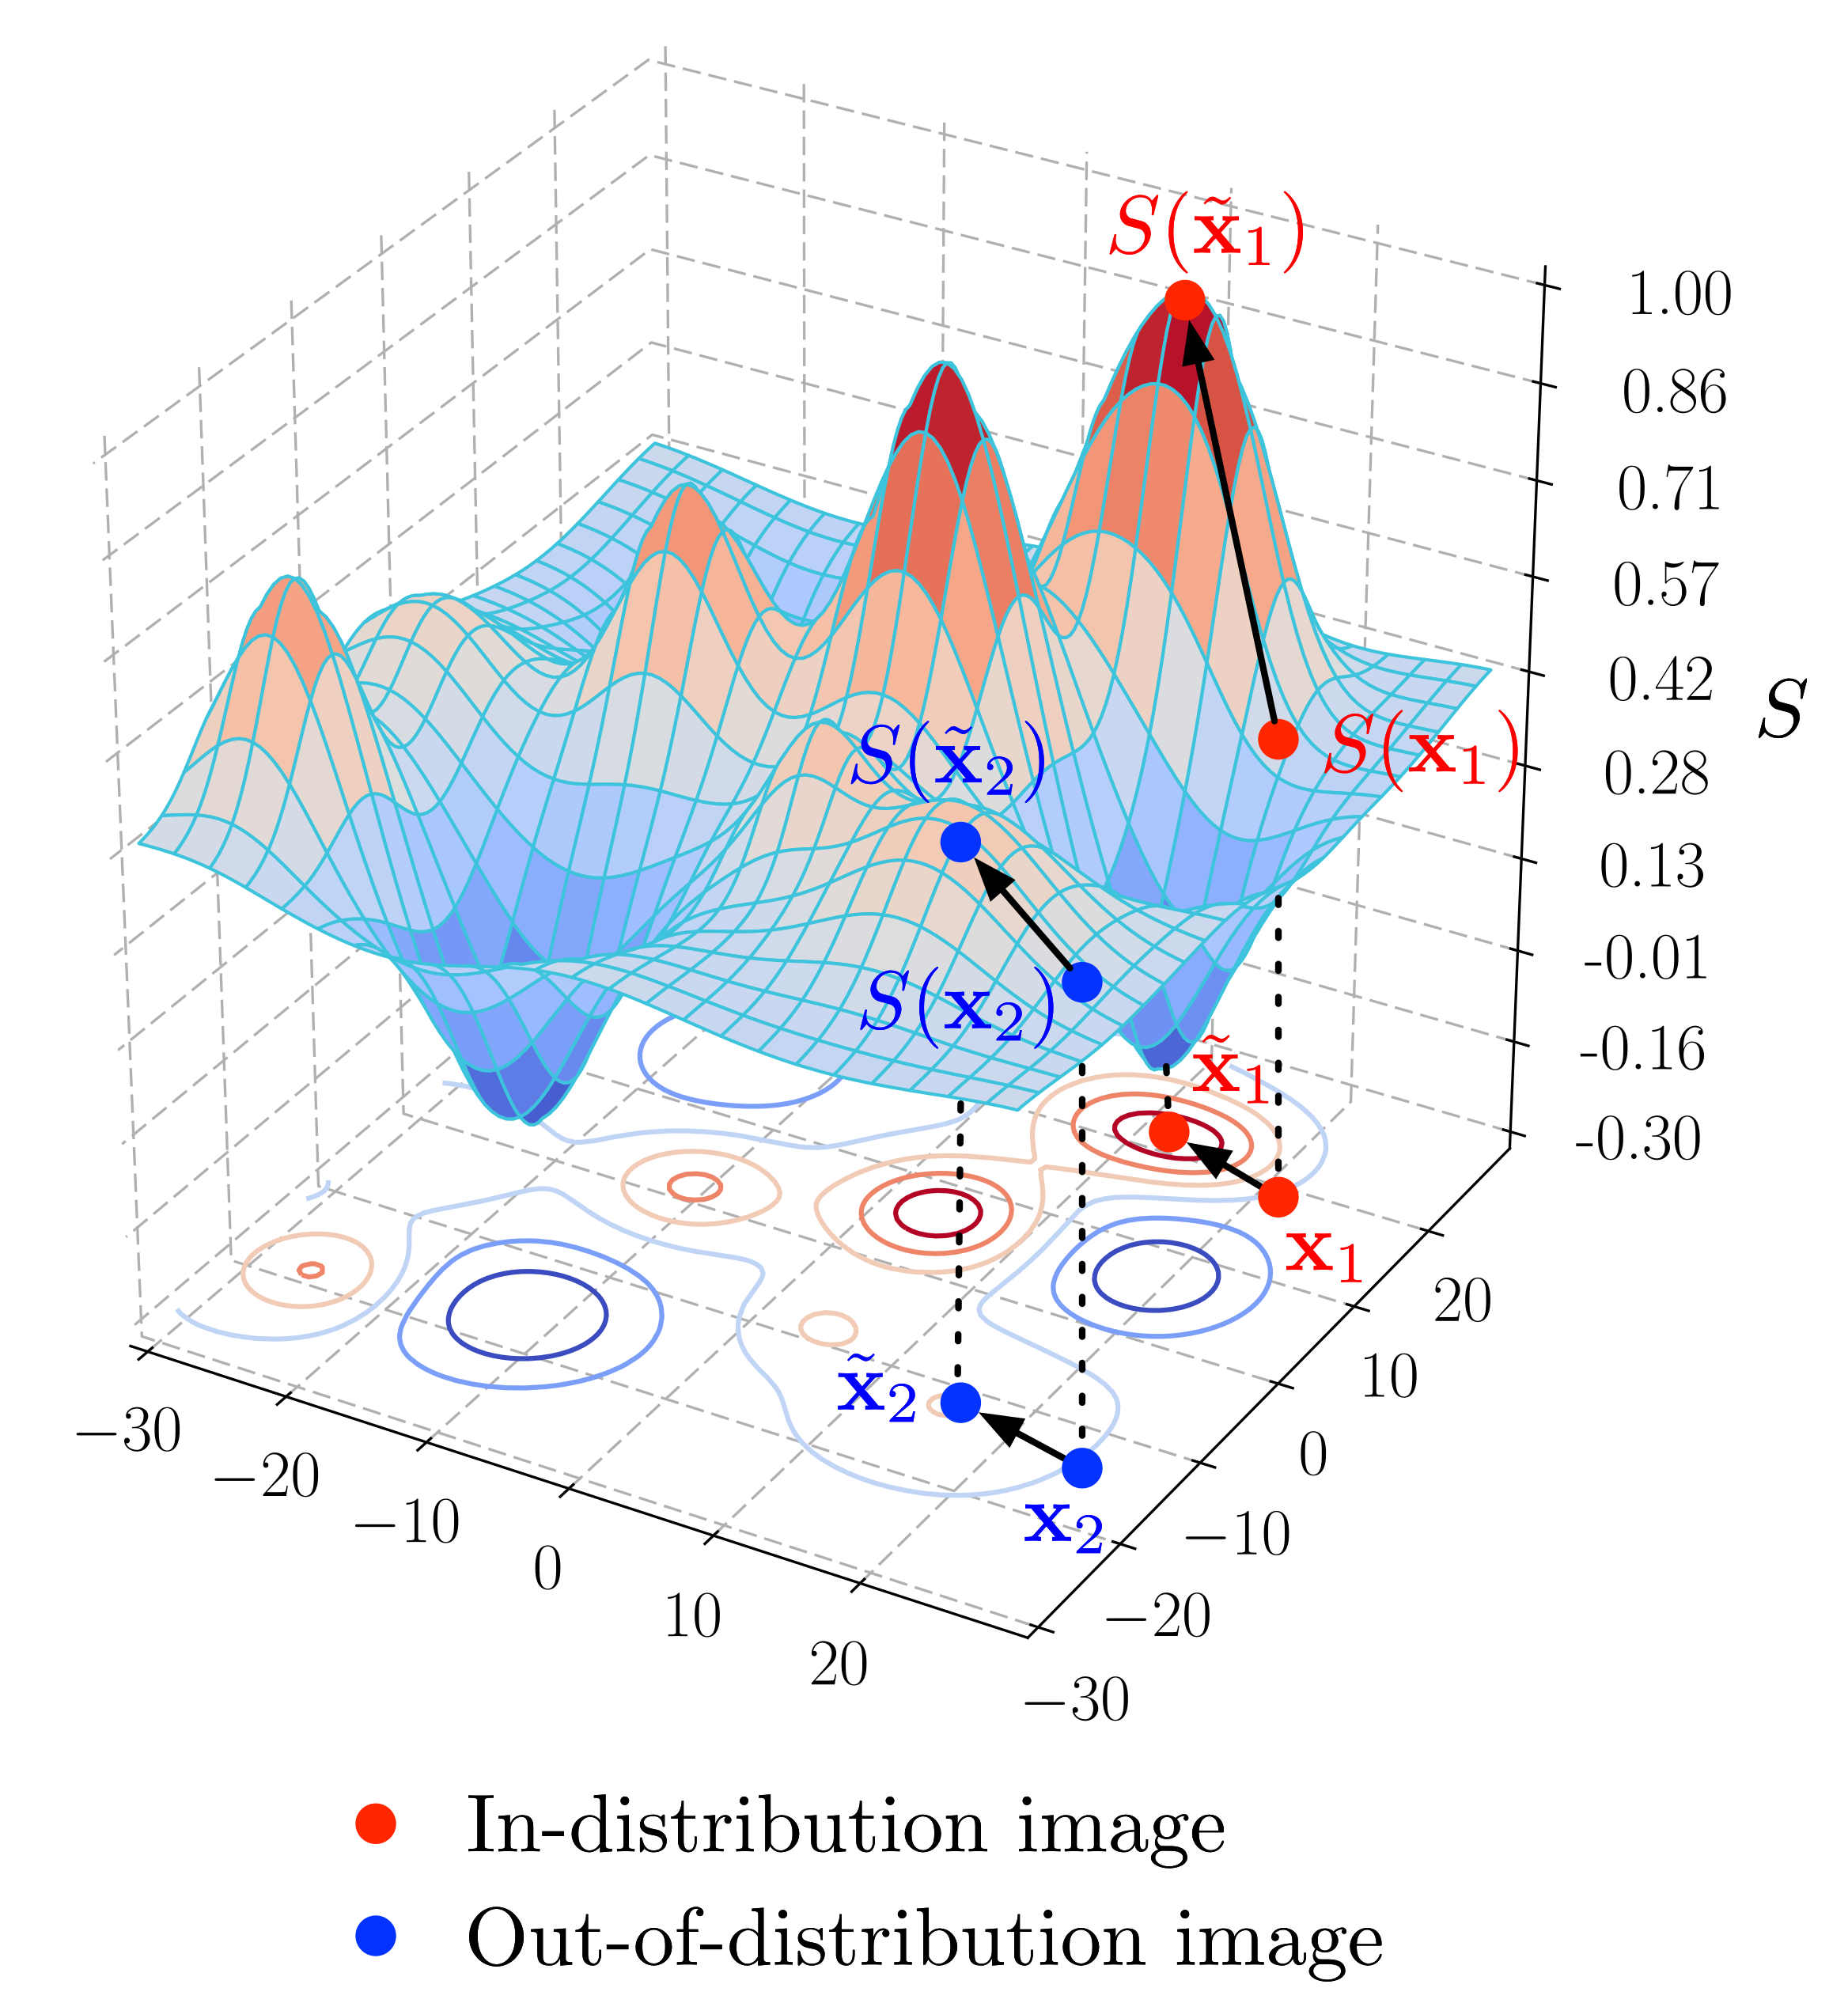
\includegraphics[width=3.25in]{figure/gradient.png}}
% \caption{Figure taken from \cite{odin}, showing the difference in gradients between \ac{id} and \ac{ood} data points}
% \label{softmaxmove}
% \end{figure}
%
% The interpretation of the temperature scaling is slightly more complex. By performing a Taylor expansion and omitting third and higher orders, we can rewrite the softmax score (i.e the value of the predicted class, the highest value) as ${S\propto {(U_{1}-U_{2}/2T)/T}}$, with $U_1$ and $U_2$ defined as follows \cite[4]{odin}:
%
%
% \begin{equation}\label{eq::u1u2}
% U_{1}(\bm{x})=\frac{1}{N-1}\sum_{i\neq\hat{y}}[f_{\hat{y}}(\bm{x})-f_{i}(\bm{x})]
% \end{equation}
%
% \begin{equation}\label{eq::u1u2}
% U_{2}(\bm{x})=\frac{1}{N-1}\sum_{i\neq\hat{y}}[f_{\hat{y}}(\bm{x})-f_{i}(\bm{x})]^{2}
% \end{equation}
%
% $\hat{y}$ is the predicted class, and is thus also the index for the highest value in $f(\bm{x})$. Thus, $U_1$ represents "the extent to which the largest unnormalized output deviates from the remaining outputs", while $U_2$ measures how the remaining outputs deviate from each other \cite[6]{odin}.
%
% \cite{odin} makes the two following observations with regards to these two values: Firstly, they find that the largest unnormalized output tends to deviate more for \ac{id} samples, making $U_1$ larger than for \ac{ood} samples, because the model is more confident in its prediction. Secondly, they find that $E[U_2|U_1]$ is larger for \ac{id} data samples than for \ac{ood} samples, which shows that \ac{id} samples have more separation in the remaining unnormalized inputs than \ac{ood} samples. 
%
% Returning to the Taylor approximated softmax score ${S\propto {(U_{1}-U_{2}/2T)/T}}$, we see that $U_1$ contributes to making the softmax score higher, while $U_2$ reduces the softmax score. Given that both these values are higher for \ac{id} data, we will want to reduce the impact of $U_2$ and increase the impact of $U_1$. As $U_1$ is divided by $T$, while $U_2$ is divided by $2T^2$, increasing the temperature achieves this, as $U_2$ will decrease much faster than $U_1$. Thus, we can see how an increased temperature increases the softmax scores for \ac{id} data, and thus increases the gap between softmax scores for \ac{id} and \ac{ood} samples, making them easier to differentiate.
%
% With these two modifications to the simple baseline proposed by \cite{oodbaseline}, \cite{odin} manages to increase the gap between the softmax scores of \ac{id} and \ac{ood} data and thus facilitates much more effective \ac{ood} detection.
% \\
%
% \subsubsection{Energy Based \ac{ood} Detection}
%
% \cite{energy} proposes using an {\it energy score} as opposed to the softmax score. They show mathematically that "the softmax confidence score is a biased scoring function that is not aligned with the density of the inputs" \cite{energy}, and thus seek to use a different measurement which is better aligned with the probability density.
%
% An energy function is a function $E(\bm{x}) : \mathbb{R}^D \rightarrow \mathbb{R}$ which maps any data point into a non-probabilistic scalar called energy. Energy values can be converted to probabilities using the Gibbs distribution defined below (equation \ref{energy}):
%
% \begin{equation} \label{energy}
%     p(y \mid \*x) = \frac{e^{-E(\*x,y)/T}}{\int_{y'} e^{-E(\*x, y')/T}}
%     = \frac{e^{-E(\*x,y)/T}}{e^{-E(\*x)/T}},
% \end{equation}
%
% This equation is quite similar to the softmax function, and we can see that by defining $E(\bm{x}, y) = -f_y(x)$. We can write the Gibbs distribution as the normal softmax output of a neural network:
%
% \begin{equation}\label{eq:softmax}
%     p(y \mid \*x) = \frac{e^{f_y(\*x)/T}}{\sum_{i}^K e^{f_{i}(\*x)/T}},
% \end{equation}
%
% By using the {\it Helmholtz free energy} measurement, we can get an energy score for each data point given to the model, which can be used to detect \ac{ood} data points. Given that we define $E(\bm{x}, y) = -f_y(x)$, we can write the Helmholtz free energy $E(\bm{x})$ as:
%
% \begin{equation}\label{eq:energy_softmax}
%   E(\*x;f)=- T\cdot \text{log}\sum_i^K e^{f_i(\*x)/T}.
% \end{equation}
%
% The authors show that when training with negative log likelihood loss, the optimization will reduce the free energy of \ac{id} data points, and that the difference  between \ac{id} and \ac{ood} energy scores is higher than the difference in softmax scores \cite{energy}. Thus, thresholding the free energy function is an effective way to separate \ac{id} and \ac{ood} data points. Furthermore, they also present a method for fine tuning a pre trained model using a loss function that is based on the energy score. By doing this, the gap between \ac{id} and \ac{ood} energy scores can be increased even further.
% \\
%
% \subsubsection{ReAct}
%
% ReAct \cite{react} is a very simple method, which also aims to increase the difference in confidence scores between \ac{id} and \ac{ood} data. It does this by rectifying high activations in the penultimate layer, which surprisingly achieves this very effectively. Figure \ref{react} gives an intuition for why this is the case:
%
% \begin{figure}[h]
% \centerline{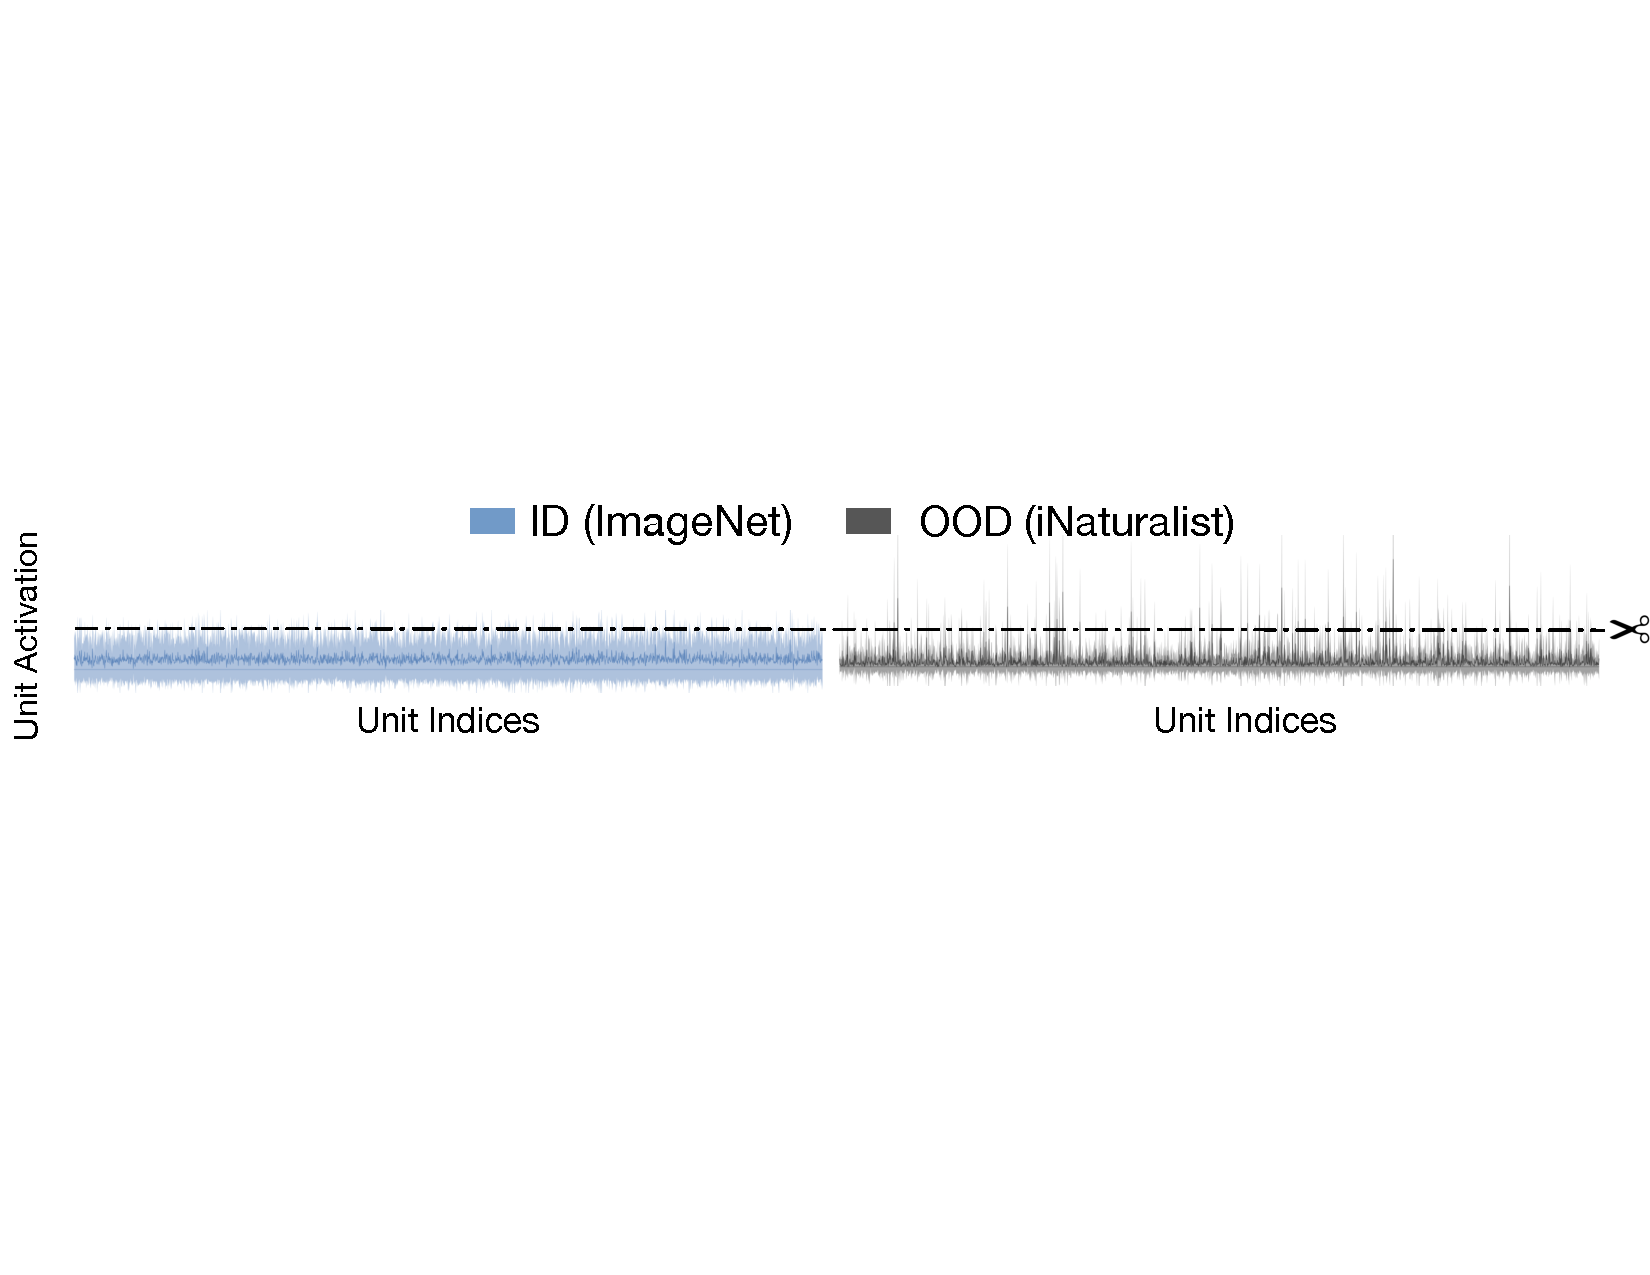
\includegraphics[width=3.25in]{figure/react.pdf}}
% \caption{Figure taken from \cite{react}, showing the activations for the nodes in the penultimate layer for \ac{id} and \ac{ood} data}
% \label{react}
% \end{figure}
%
% From this, we see that \ac{ood} samples have much more irregular activations, with a higher variance and many high value outliers. This gives an explanation for why \ac{ood} samples produce highly confident softmax scores: sharp positive outliers manifest in the model output, producing high logits in the output layer \cite{react}. By using a positive upper limit to rectify these outliers, we can remove their impact and reduce the confidence for \ac{ood} data.
%
% This gives rise to a very simple \ac{ood} detector: Let us denote the feature vector of the penultimate layer as $h(\bm{x})$, where $\bm{x}$ is the input feature vector. The logits of the network would be calculated by the function
%
% \begin{equation}\label{dog}
%   f(\bm{x}) = W \, h(\bm{x}) + \bm{b},
% \end{equation}
%
% where $W$ is a matrix which projects $h(\bm{x})$ down to the output space. $h(\bm{x})$ is the vector which contains the high activations for \ac{ood} data, so by rectifying this vector with $\text{ReAct}(\bm{x}; c) = min(\bm{x}, c)$ for a $c > 0$, we can remove these outlier activations. We then get
%
% \begin{equation}\label{dog}
%   \bar{h}(\bm{x}) = \text{ReAct}(h(\bm{x}; c),
% \end{equation}
%
% which gives us the new output logits 
%
% \begin{align}
% f^{\text{ReAct}}(\*x;\theta) = \*W^\top \bar h(\*x) + \mathbf{b}.
% \end{align}
%
% These logits can be used by any other \ac{ood} method which uses the output values to separate \ac{id} and \ac{ood} samples \cite{react}:
%
% \begin{align}
% \label{eq:threshold}
%     g(\bm{x}; f^\text{ReAct}, \delta)=\begin{cases} 
%         \text{in } & S(\bm{x};f^\text{ReAct})\ge \delta \\
%         \text{out} & S(\bm{x};f^\text{ReAct}) < \delta 
%    \end{cases},
% \end{align}
%
% This simple methods performs well on many benchmarks, with the added benefit that it can be combined with many other methods. For example, we can use ODIN or Energy with output scores calculated using ReAct instead of unrectified outputs, which leads to improvements over the methods used by themselves.
% \\
%
% \subsubsection{Virtual Outlier Synthesis (VOS)}
%
% Generating outliers to expose to the model during training is another way to reduce the model's confidence on \ac{ood} data. However, creating realistic \ac{ood} data points can be difficult, especially if the input space is of a high dimension, such as in image classification. \cite{vos} presents a more tractable method, which synthesizes outliers not in the input space, but in the feature space, which can be of a much lower dimensionality.
%
% In this lower dimension space, previously intractable methods are now less computationally expensive. To synthesize outliers, \cite{vos} simply estimates class conditional Gaussian distributions by computing empirical class means and covariances, and sample outliers from the class boundaries between these Gaussians.
%
% Using these outliers, they present a "unknown-aware training objective", which can be used during training to maximize the separability between \ac{id} and \ac{ood} data during inference.
% \\

\subsubsection{GradNorm}

As opposed to using the feature or output space, GradNorm \cite{gradnorm} attempts to use the gradient space of a network to calculate \ac{ood}-ness. They find that the gradients of the weights actually contain valuable information that allows for effective separation of \ac{id} and \ac{ood} samples, and perform ablation studies which show that this methods outperforms many other methods, including the previously mentioned ODIN and Energy methods.

The gradients are calculated with regards to the Kullback-Leibler divergence between the softmax values and a uniform distribution. An important distinction from other methods is that all the softmax values are used, as opposed to the {\it softmax score} which would be only the score of the predicted class. Thus, this method captures information about the uncertainty across all categories, as opposed to just the most likely class \cite[3]{gradnorm}. Once the gradients have been calculated, the threshold is simply done on the $L_p$-norm of these gradients, giving us the following thresholding function \cite{gradnorm}:

\begin{equation}
\label{eq:score}
    S(\*x) = \lVert\frac{\partial D_\text{KL}(\*u~\lVert~\text{softmax}(f(\*x))}{\partial \*w}  \rVert_p
\end{equation}

As shown in figure \ref{gradnorms}, we see that the gradient norms are consistently lower for \ac{ood} data (gray) than \ac{id} data (blue).

\begin{figure}[h]
\centerline{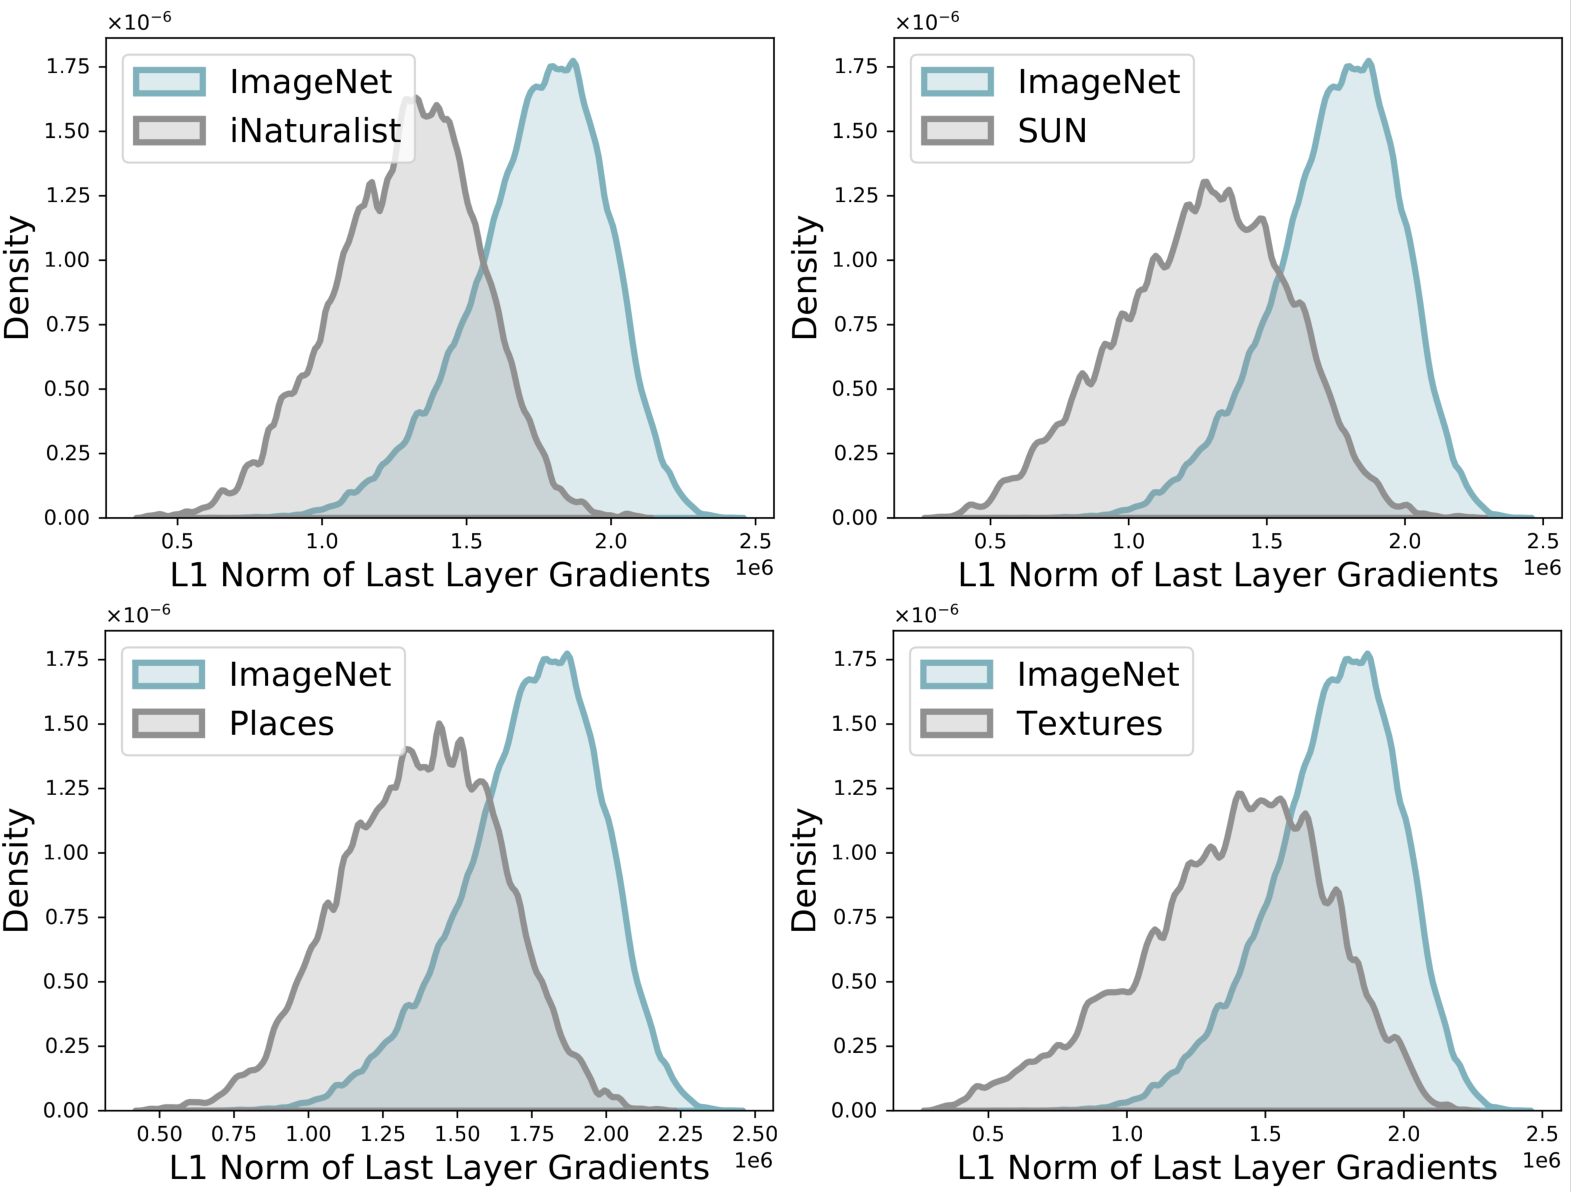
\includegraphics[width=3.25in]{figure/gradnorm.pdf}}
\caption{Figure taken from \cite{gradnorm}, showing the difference in gradient norms between \ac{id} and \ac{ood} data}
\label{gradnorms}
\end{figure}

\cite{gradnorm} find that it is sufficient to only calculate the gradients for the last layer of the network, and that the $L_1$-norm performs the best, as it weights all gradients equally, as opposed to higher norms which place more importance on larger values.

In their mathematical analysis, they show that GradNorm captures joint information from both the feature and output space. By decomposing the $L_1$-norm of gradients of weights of the last layer with regards to the Kullback-Leibler divergence, they reach the following equality:

\begin{equation}
S(\bm{x}) = \frac{1}{CT}  \left(\sum_{i=1}^m |x_i|\right) \left(\sum_{j=1}^C \left|1 - C \cdot \frac{e^{f_j / T}}{\sum_{j=1}^C e^{{f_{j}} / T}}\right|\right)
\label{eq:decomp}
\end{equation}

From this, we see that $S(\bm{x})$ is a product of a factor which is simply the $L_1$-norm of the feature vector $\bm{x}$, and another term which captures information about the softmax values in the output space.
\\


\subsubsection{Virtual Logit Matching (ViM)} \label{section:vim}

\cite{vim} attempts to improve \ac{ood} detection by calculating a score based on the feature, the logit and the softmax probability at once, as opposed to just one of them. By looking at all three elements in conjunction, they see an increase in performance over models which only rely on a single input source (such as the previously mentioned ODIN).

The reasoning behind not just looking at the logits or softmax probability is that there is a lot of information that is lost when going from features to logits \cite{vim}. Once we project the features down to logits, we have only class dependent information, and have lost the class agnostic information which is contained within the features. To show how this information is lost, the authors give an example based on null space analysis \cite{nusa}:

Let us assume that we have a simplified network with only a single layer. Then, we have $\hat{\bm{y}} = W \bm{x}$, where $\hat{\bm{y}}$ is the vector containing the logits, $\bm{x}$ is the feature vector of the input (with an additional 1 for the bias term) and $W$ is the matrix containing the weights and biases transforming the feature vector into logits. A null space $\text{Null}(W)$ of a matrix $W$ is the set of all vectors that map to the zero vector, such that $W \bm{a} = \bm{0} \iff \bm{a} \in \text{Null}(W)$. The null space of a matrix may be trivial (empty), but a matrix which projects vectors to a lower dimension have non-trivial null spaces. Given that the final layer of a neural network projects down to logits, which are the same dimension as the number of classes, this will almost always be the case. Because of the distributivity of matrix multiplication, we have the following:

\begin{equation}
W (\bm{x} + \bm{a}) = W \bm{x} + W \bm{a} = W \bm{x} + \bm{0} = W \bm{x}
\label{matrix}
\end{equation}

The vector $\bm{x}$ can be decomposed into $\bm{x}^W + \bm{x}^{\text{Null}(W)}$, where $\bm{x}^W$ is the projection of $\bm{x}$ onto the column space of $W$ and $\bm{x}^{\text{Null}(W)}$ is the projection of $\bm{x}$ onto the null space of $W$. It follows from this and equation \ref{matrix} that when going from features to logits using the projection $W \bm{x}$, we lose all information contained in $\bm{x}^{\text{Null}(W)}$. \cite{nusa} shows how this can be exploited by adversarial methods, by creating images with added noise derived from the null space of a matrix within the network, which are classified as if the noise was not present, despite having no resemblance to the original image. See figure \ref{dog}.

\begin{figure}[hbt]
    \centering
    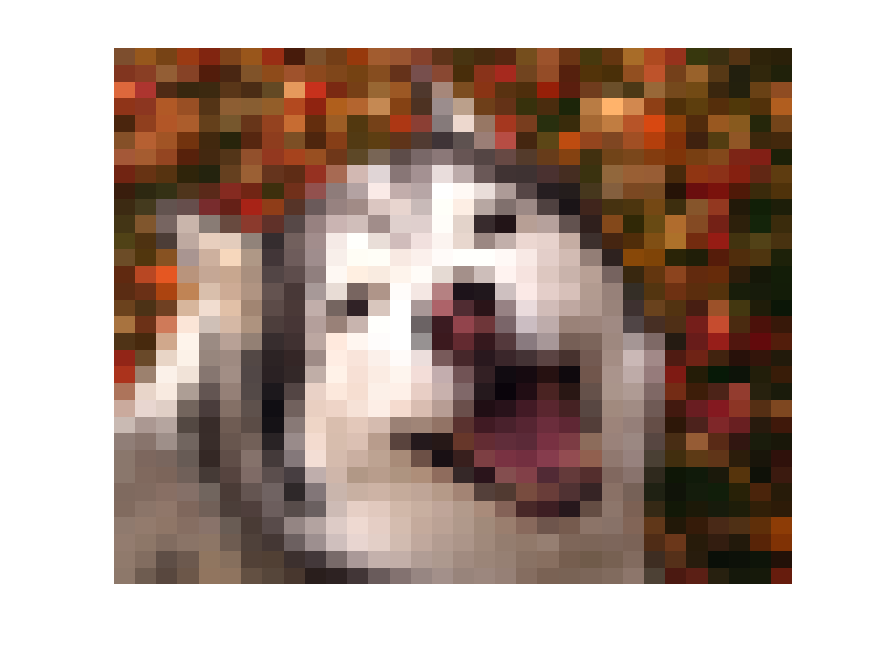
\includegraphics[width=0.32\linewidth,trim={1.25cm 1.25cm 1.25cm 1.25cm},clip]{figure/OrigImage.pdf}
    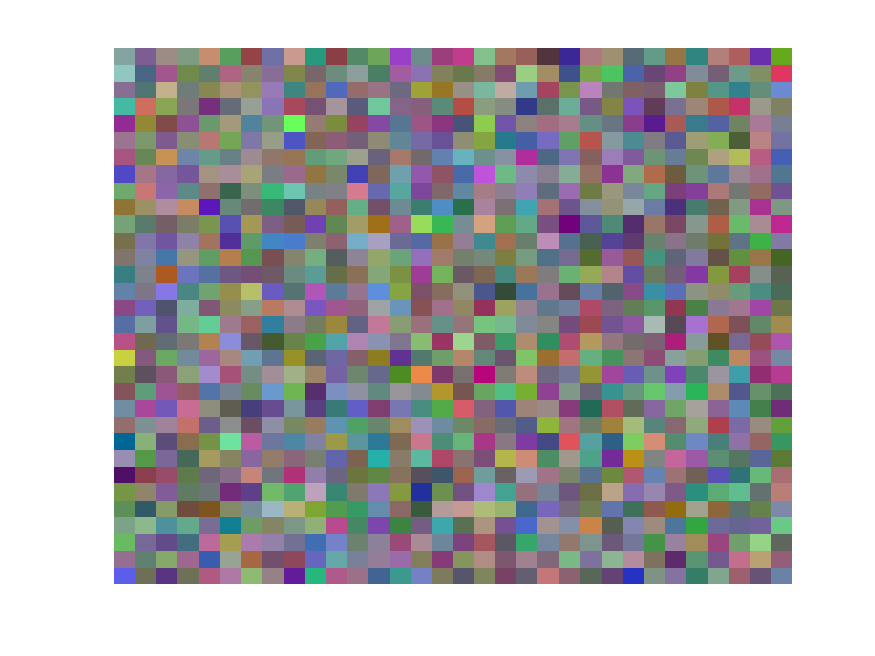
\includegraphics[width=0.32\linewidth,trim={1.25cm 1.25cm 1.25cm 1.25cm},clip]{figure/PureNoise.pdf}
    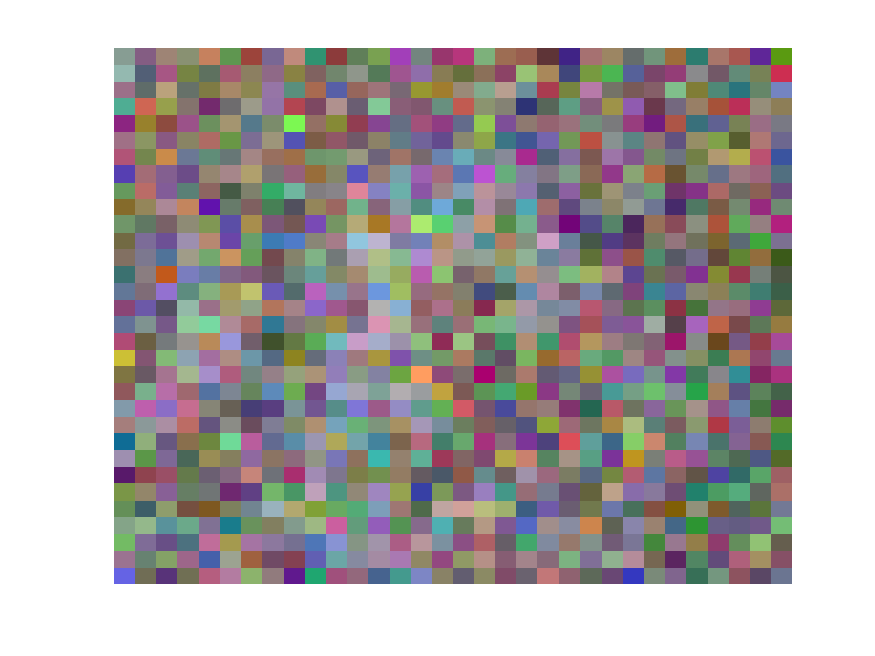
\includegraphics[width=0.32\linewidth,trim={1.25cm 1.25cm 1.25cm 1.25cm},clip]{figure/NoiseAdded.pdf}
    \caption{Image taken from \cite{nusa}. Left: Original image. Center: Additive null space noise. Right: Final image, indistinguishable from original image according to the network the noise in the center column is sampled from.}
    \label{dog}
\end{figure}

From this, we can see that potentially large amounts of information can be lost when going from features to logits. Using this information, it is also possible to perform \ac{ood} detection, as shown by \cite{nusa}. Another method which uses the features performs \ac{pca} and looks at the residual information lost when using the first $N$ principal components \cite{subspace}. However, the information in the features is still class agnostic, and \cite{vim} aims to go beyond using just one input source and combine several elements of the network.

To do this, they propose using a {\it Virtual Logit}. The Virtual Logit is calculated as follows: First, they center the feature space, so that "it is bias free in the computation of logits" \cite{vim}. They then perform \ac{pca} as in \cite{subspace}, and calculate the residual of $\bm{x}$ with regards to the principal components, which is the projection $\bm{x}$ onto the null space of the principal subspace $P$. The residual represents the information lost when using the projection $P$.

\begin{equation}
\text{Residual}(x) = || \bm{x}^{\text{Null}(P)}||
\label{virtuallogit}
\end{equation}

This value is scaled based on the average values of the maximum logit across the dataset, and is appended to the rest of the logits as a Virtual Logit:

\begin{equation}
l_0 := \alpha || \bm{x}^{\text{Null}(P)}||
\label{virtuallogit}
\end{equation}

This now takes part in the computation of the softmax values, and thus is affected by the size of the rest of the logits. They call the softmax value of the Virtual Logit the {\it ViM score}. In this way, the ViM score represents the size of the residual in comparison with the predictions of the model. If the model is very confident, then the norm of the residual will be small in comparison, and the ViM score will be low. If the residual is very large, the ViM score will be higher, and more indicative of an \ac{ood} sample. In this way, \cite{vim} have combined information from the feature, the logit and the softmax probability level to perform \ac{ood} detection.

\subsubsection{COMBOOD}

\texttt{COMBOOD} \cite{combood} is another \ac{ood} detection method which combines information from different sources to increase performance. Unlike \ac{vim}, which combines different internal signals from the network, \texttt{COMBOOD} combines information from two different metrics calculated from the feature space. The two metrics are Mahalanobis distance and nearest neighbour distance, which have both seen decent performance on their own \cite{nearestneighbour, mahalanobis}. \cite{combood} builds on these works by showing that their combination into one single score can increase performance far above either one. Indeed, the performance of \texttt{COMBOOD} is \acl{sota}, being the highest performing \ac{ood} detector on the ImageNet200 and ImageNet1K benchmarks in the OpenOOD framework.\footnote{https://zjysteven.github.io/OpenOOD/}

To understand how \texttt{COMBOOD} works, we must first understand how Mahalanobis and nearest neighbour distance work as \ac{ood} detectors. Mahalanobis distance assumes that the features generated by the network are distributed as a multivariate Gaussian, and calculates the distance based on the mean and standard deviations of this Gaussian. This method is a generalization of calculating the Z-score for a univariate Gaussian, and has the following form, given a mean $\bm{\mu}$ and covariance matrix $\Sigma$, calculated over the \ac{id} training set:

\begin{equation}
    \text{Mahalanobis}(\bm{x}) = \sqrt{(\bm{x} - \bm{\mu})^T\Sigma^{-1}(\bm{x} - \bm{\mu})}
\end{equation}

Nearest neighbour distance has the advantage that it does not impose any assumptions about the distribution of the feature space, and is thus non-parametric. The k-nearest neighbour distance, is simply the distance from a given datapoint to the k'th nearest neighbour in feature space. \cite{nearestneighbour}, which used this distance metric for \ac{ood} detection, normalized the features and used Euclidean distance as the distance metric, giving us the following equation:

\begin{equation}
    \text{NN}(\bm{x}) = \| \bm{x^*} - \bm{z}_k \|_2,
\end{equation}

where $\bm{x^*}$ is the normalized feature $\bm{x}$ and $\bm{z}_k$ is the k'th nearest neighbour from the \ac{id} training set.

\texttt{COMBOOD} combines these metrics by computing "confidence scores" for each distance, which are then added together to produce a final score. In addition, they find that by using different feature extracting methods for each of the different methods, their combined performance can be enhanced considerably, concluding that "COMBOOD performs best when the nonparametric and the parametric components use different feature extraction strategies, penultimate layer embeddings for the former and global extrema of the features for the latter" \cite{combood}.

\section{Related work} \label{section:relatedwork}

In a broad sense, this work is about \ac{ood} detection. In this way, the field of \ac{ood} detection, and methods described in the preceding sections, can be thought of as constituting the related work. However, more specifically, I attempt to use \ac{xai} methods to enhance \ac{ood} detection performance, and thus we may look towards previous work which has attempted a similar combination.

While the combination of \ac{xai} and \ac{ood} detection has been explored in many previous works, the majority of them focus on explaining why a data point was marked as \ac{ood}, as opposed to using \ac{xai} to aid the detection itself. Works like \cite{uncertainty}, \cite{generalxaiforood} and \cite{tallon2020explainable} are papers which combine \ac{xai} and \ac{ood} for this purpose. Within network security, \ac{xai} has been as part of anomaly detection systems to detect malicious or faulty network traffic. Here, it has been used to explain detections (\cite{idsxai}, \cite{mahbooba}), but also to aid in detection itself by inspecting the explanations of the detection system (\cite{tcydenova2021detection}, \cite{dnsxai}). These methods thus use \ac{xai} to aid \ac{ood} detection in a similar manner to my work, however they are strictly focused on sequential network traffic data as opposed to images, and are mostly concerned with detection "unnatural" data samples such as intentionally malicious traffic or that generated by faulty equipment, as opposed to natural \ac{ood} data caused by semantic or covariate shift occurring when a model is deployed.

\cite{martinez} is the most relevant previous work. Here, the authors explicitly aim to use \ac{xai} to improve \ac{ood} detection on images. They do this by looking at saliency maps produced by a \ac{gradcam}-based \ac{xai} method (section \ref{section:gradcam}) during inference, i.e the heatmaps that explain which parts of the image was most influential to classify the image as a specific class. Using these heatmaps, they perform distance-based \ac{ood} detection (section \ref{section:distancebasedood}): By collecting all explanations for each image in the \ac{id} dataset, they are able to construct archetypical explanations, and can make clusters of explanations. To perform \ac{ood} detection, they simply compare the explanation of a new data point to the clusters of archetypical explanations, and mark it as \ac{ood} if it has a distance which is over a certain threshold.

This method performs decently on toy benchmarks, achieving scores similar to \ac{sota} methods when using {\it Fashin MNIST} as \ac{id} and {\it MNIST} as \ac{ood}. However, this method fails catastrophically in more complicated scenarios, achieving an \ac{auroc} score of only $52\%$ on {\it CIFAR10} vs {\it SVHN}, which is only marginally better than pure guessing and far below any other method. The paper thus ends with the authors concluding that "OoD detection approaches that are specifically designed for the purpose achieve in general better detection scores at the cost of an additional computational burden in the model’s construction" \cite{martinez}.

For more potential related work, we can look to OpenOOD (\cite{openood}), which aims to provide a comprehensive benchmark of all relevant methods in the field of \ac{ood} detection. Out of all 41 \ac{ood} detection methods included in this benchmark, there are no methods which use \ac{xai}. However, as many \ac{xai} methods utilize the gradients of the network to generate saliency values, we could also consider \ac{ood} detection models which utilize gradients in some form as tangentially related to this thesis. In this regard \cite{gradnorm} is related, as they utilize the norm of the gradients of the network with respect to the Kullback-Leibler distance between the outputs and a uniform distribution.

From the absence of any relevant method utilizing \ac{xai} in OpenOOD and from the poor results of \cite{martinez}, we can see that the potential for a truly effective \ac{ood} detection system using \ac{xai} has not been fully realized in any previous work.

\section{Summary}

In this chapter, I have given a thorough introduction.

\chapter{Methodology} \label{chapter:methodology}

As shown in the preceding chapter, there exists a plethora of \ac{xai} methods, which exploit gradient information, differences in output scores when altering model inputs, marginal contributions of input features, as well as many other intricacies of deep learning models. The core idea of this master thesis is that these methods, in their attempt to explain a model decision, may also inadvertently extract information which is valuable for \ac{ood} detection. Thus, there may be an unexplored potential in these methods to function not just as explanations, but also as classifiers which allow us to separate \ac{id} and \ac{ood} data. Intuitively, we might expect the explanations to be more spread out on \ac{ood} images, given that there are (by definition) no objects of interest in the image that the model can definitely be said to focus on. In contrast, we might expect an explanation on an \ac{id} image to be more focused on a specific area, which contains an object of interest. Furthermore, given that saliency methods give a numerical value to each region of the image, we might be able to extract information about the "\ac{ood}-ness" of an image by inspecting the magnitudes of these values. Intuitively, it may be the case that such values should be lower for \ac{ood} than \ac{id}, reflecting the higher uncertainty present in \ac{ood} data.

% As an example, let us consider \ac{gradcam}. As explained in section \ref{section:gradcam}, \ac{gradcam} uses the gradients of the weights within the final convolutional layer with regard to the output prediction, along with the final feature maps, to generate an explanation.

\section{Proposed \ac{xai} frameworks for \ac{ood} detection} \label{section:methods}

With the preceding intuitions in mind, I present three frameworks for \ac{ood} detection which utilize \ac{xai} methods as part of their detection pipeline.

\subsection{Stand-alone saliency framework: Aggregate of Saliency} \label{section:saliencyagg_method}

As we have seen from section \ref{section:relatedwork}, there has been little research into using explanations for \ac{ood} detection, aside from the work of \cite{martinez}. Thus, I begin by presenting a simple framework which uses saliency values generated by \ac{xai} methods to calculate an \ac{ood} score.

As mentioned previously, the field of \ac{ood} detection started with the simple baseline introduced by \cite{oodbaseline}, which simply uses the \ac{msp} (i.e the confidence score of the predicted class) as a way to measure \ac{ood}. Later, it was shown that using the \ac{mls} could also serve as an effective baseline. As such, I propose a similarly simple baseline when using explanations for \ac{ood} detection. The analogue of the maximum logit in an \ac{xai} context can reasonably be said to be the explanation generated of the predicted class (the class corresponding to the maximum logit). As explained previously, this explanation will take the form of an $n \times m$ saliency map. This saliency map is not a single scalar value, and does thus not make a suitable \ac{ood} score by itself. Instead, we may perform some form of aggregation on the saliency map (such as taking the mean, the vector norm, the variance or some other form), and use this as the \ac{ood} score.

The intuition for this method is informed by the fact that there are many forms of aggregation over saliencies which one might reasonably expect to be different for \ac{id} and \ac{ood} data. As an example, let us consider the implications of aggregating in some way which captures the magnitude of the saliencies, such as the {\it mean}, the {\it vector norm}, or the {\it max value}. When we generate a saliency map using the predicted class, the \ac{xai} saliency method attempts to calculate a measure of importance for each region of the input image, with regard to this class. For \ac{id} data, as long as the model predicted correctly, we know that there really are regions of the input image which contain the predicted class. If we instead are looking at semantically shifted \ac{ood} data, we know that no input image contains any of the \ac{id} classes. Thus, when a neural network makes a prediction on such a data point, it will always be wrong, because it will always predict one of the \ac{id} classes. By generating a saliency map of this prediction, we are asking a method to decide how each region contributed to a false decision. Given that there are no objects of the predicted class, in any region, we may reasonably assume that the saliency values are very different than in an \ac{id} case, where such objects actually are present.

\subsubsection{Intuition 1: Magnitude of saliencies may be different}

To further justify this intuition, I will present a simple example scenario (figure \ref{fig:meansaliency}) where one might expect the \ac{id} saliencies to be higher than the \ac{ood} saliencies. Here, I imagine a model which has been trained to differentiate between different breeds of dogs. In the first case, it is given an image of a dog, and a prediction of "English Foxhound" is made, which happens to be correct. Generating an explanation for this prediction, each region of the image is given a measure of importance, calculated using gradient information, differences in prediction score on counterfactual examples or by other means. As there actually is an English Foxhound in the image, we may expect that these methods generate saliencies which have a magnitude which is higher than if there was no dog present.

\begin{figure}[H]
    \begin{center}

    \begin{tikzpicture}[
    SIR/.style={rectangle, draw=black!80, thick, minimum size=5mm},
    ]

    \node[SIR, label={[align=center]Image with dog present,\\correctly classified as\\"English Foxhound"}] (idimg) {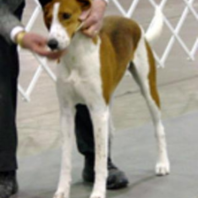
\includegraphics[width=0.25\textwidth]{figure/meansaliency/meansaliency0.png}};
    \node[SIR, label={[align=center]Image without dog\\present, wrongly\\classified as "Samyoed"}] (oodimg) [right=of idimg] {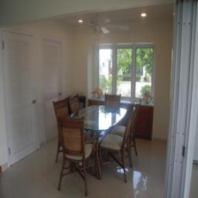
\includegraphics[width=0.25\textwidth]{figure/meansaliency/meansaliency2.png}};

    \node[SIR] (idsal) [below=1.5cm of idimg] {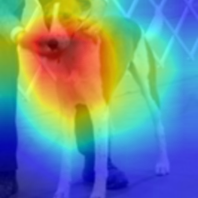
\includegraphics[width=0.25\textwidth]{figure/meansaliency/meansaliency1.png}};
    \node[SIR] (oodsal) [below=1.5cm of oodimg] {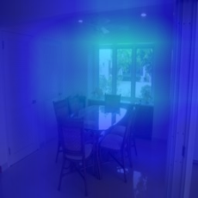
\includegraphics[width=0.25\textwidth]{figure/meansaliency/meansaliency3.png}};

    \node[SIR] (idmean) [below=1.5cm of idsal] {Mean saliency = $0.152$};
    \node[SIR] (oodmean) [below=1.5cm of oodsal] {Mean saliency = $0.034$};

    \draw[->, very thick] (idimg.south)  to node[midway, fill=white, align=center] {Generate \ac{xai} heatmap\\of model prediction} (idsal.north);
    \draw[->, very thick] (oodimg.south)  to node[midway, fill=white, align=center] {Generate \ac{xai} heatmap\\of model prediction} (oodsal.north);

    \draw[->, very thick] (idsal.south)  to node[midway, fill=white, align=center] {Calculate average value\\of heatmap} (idmean.north);
    \draw[->, very thick] (oodsal.south)  to node[midway, fill=white, align=center] {Calculate average value\\of heatmap} (oodmean.north);

    \node[SIR, align=left, draw=id, fill=id!30] (iddecision) [below=of idmean] {Above threshold:\\classified as \ac{id}};
    \node[SIR, align=left, draw=far, fill=far!30] (ooddecision) [below=of oodmean] {Below threshold:\\classified as \ac{ood}};

    \draw[->, very thick] (idmean.south)  to node[midway, fill=white] {Compare with threshold} (iddecision.north);
    \draw[->, very thick] (oodmean.south)  to node[midway, fill=white] {Compare with threshold} (ooddecision.north);

    \begin{scope}[shift={($(oodsal.east)+(0.1cm,0.25\textwidth / 2)$)}]
        \pgfplotscolorbardrawstandalone[
        colormap name=turbo,
        point meta min=0,
        point meta max=0.345,
        colorbar style={
            height=0.25\textwidth, % Match the height of the images
            width=0.4cm, % Desired width of the colorbar
            ytick={0, 0.173, 0.345},
            % yticklabels={Low, Medium, High},
        }]
    \end{scope}
    \end{tikzpicture}
    \caption[Mean Saliency visual explanation]{Figure showing the functioning of the Aggregate of Saliency \ac{ood} detector, using mean as the aggregation, in a hypothetical scenario where a model trained on images of dogs is shown an image with no dogs present. The heatmaps here show the maximum value of both saliency maps as dark red, reflecting the lack of normalization}
    \label{fig:meansaliency}
    \end{center}
\end{figure}

In the second case, the model is given an image without any dogs present. Given that there is no class for images without dogs in them, the model will classify the image as one of the possible dog breeds. In this case, the model predicted the class of "Samoyed", a decision which can be considered essentially arbitrary. When a explanation is generated for this decision, the methods for calculating importance scores will most likely assign saliencies to most regions, given that no region contains a dog. As such, if we calculate mean saliencies for both the image with the dog and the one without, we expect the image with the dog to have a higher mean saliency. As long as we work with semantically shifted \ac{ood} data, it will always be the case that the prediction on \ac{ood} data is wrong, and thus we may also expect that the generated explanations in general output smaller saliencies.

On the contrary, we could also expect that \ac{ood} saliency maps have {\it higher} magnitudes than \ac{id} saliency maps. As has been well documented, neural networks behave unpredictably when exposed to examples far from their training distribution \cite{nguyen2015deepneuralnetworkseasily, geirhos2020shortcut, goodfellow2015explainingharnessingadversarialexamples}. Thus, it is not unreasonable to expect that explanations based on this unpredictable behaviour may also be unstable and unpredictable. This instability could lead to large outliers in saliency maps, which would give larger magnitudes when compared to \ac{id} data points. Figure \ref{fig:meansaliencyless} shows an imagined example scenario where this could be the case. Here, we imagine that the same dog breed classifier is shown two images: the first an image of a Border Terrier in a park, an scenario which we could assume is quite common in the training dataset. The second is a night time picture of a illuminated archway, an image which is very far away from the training distribution of the model, and contains many sharp changes in pixel intensity. In such a scenario, it is possible that a network will behave unpredictably, which may be reflected in the saliency map of the model. As explained in section \ref{section:xaimethodsbackground}, methods such as \ac{gradcam}, \ac{gbp} and integrated gradients use gradient information from the network, which may be affected by sharp activations in the internals of the model.


\begin{figure}[H]
    \begin{center}

    \begin{tikzpicture}[
    SIR/.style={rectangle, draw=black!80, thick, minimum size=5mm},
    ]

    \node[SIR, label={[align=center]Image with dog present,\\correctly classified as\\"Border Terrier"}] (idimg) {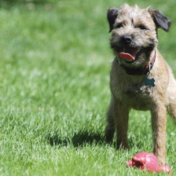
\includegraphics[width=0.25\textwidth]{figure/meansaliencyless/id_less_magnitude-img0.png}};
    \node[SIR, label={[align=center]Image without dog\\present, wrongly\\classified as "Dingo"}] (oodimg) [right=of idimg] {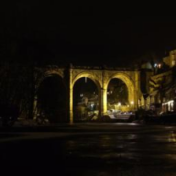
\includegraphics[width=0.25\textwidth]{figure/meansaliencyless/id_less_magnitude-img2}};

    \node[SIR] (idsal) [below=1.5cm of idimg] {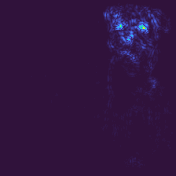
\includegraphics[width=0.25\textwidth]{figure/meansaliencyless/id_less_magnitude-img1.png}};
    \node[SIR] (oodsal) [below=1.5cm of oodimg] {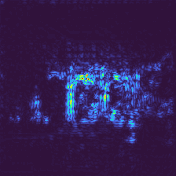
\includegraphics[width=0.25\textwidth]{figure/meansaliencyless/id_less_magnitude-img3.png}};

    \node[SIR] (idmean) [below=1.5cm of idsal] {Mean saliency = $0.23$};
    \node[SIR] (oodmean) [below=1.5cm of oodsal] {Mean saliency = $0.69$};

    \draw[->, very thick] (idimg.south)  to node[midway, fill=white, align=center] {Generate \ac{xai} heatmap\\of model prediction} (idsal.north);
    \draw[->, very thick] (oodimg.south)  to node[midway, fill=white, align=center] {Generate \ac{xai} heatmap\\of model prediction} (oodsal.north);

    \draw[->, very thick] (idsal.south)  to node[midway, fill=white, align=center] {Calculate average value\\of heatmap} (idmean.north);
    \draw[->, very thick] (oodsal.south)  to node[midway, fill=white, align=center] {Calculate average value\\of heatmap} (oodmean.north);

    \node[SIR, align=left, draw=id, fill=id!30] (iddecision) [below=of idmean] {Below threshold:\\classified as \ac{id}};
    \node[SIR, align=left, draw=far, fill=far!30] (ooddecision) [below=of oodmean] {Above threshold:\\classified as \ac{ood}};

    \draw[->, very thick] (idmean.south)  to node[midway, fill=white] {Compare with threshold} (iddecision.north);
    \draw[->, very thick] (oodmean.south)  to node[midway, fill=white] {Compare with threshold} (ooddecision.north);

    \begin{scope}[shift={($(oodsal.east)+(0.1cm,0.25\textwidth / 2)$)}]
        \pgfplotscolorbardrawstandalone[
        colormap name=turbo,
        point meta min=0,
        point meta max=0.82,
        colorbar style={
            height=0.25\textwidth, % Match the height of the images
            width=0.4cm, % Desired width of the colorbar
            ytick={0, 0.41, 0.82},
            % yticklabels={Low, Medium, High},
        }]
    \end{scope}
    \end{tikzpicture}
    \caption[Mean Saliency visual explanation]{Figure showing the functioning of the Aggregate of Saliency \ac{ood} detector, using mean as the aggregation, in a hypothetical scenario where a model trained on images of dogs is shown an image with no dogs present. As opposed to the previous figure, here we assume that \ac{id} samples have lower mean values on average, and as such the thresholding is inverted.}
    \label{fig:meansaliencyless}
    \end{center}
\end{figure}

\subsubsection{Intuition 2: Statistical dispersion of saliencies may be different}

Apart from aggregations which convey information about the magnitude of the saliencies, we may also expect the variation or dispersion of the saliencies to be different between \ac{id} and \ac{ood} data. We might expect the heatmap on \ac{ood} data to be less concentrated and more evenly spread out, given that there are no actual objects of interest present. This would give \ac{ood} data points a low variance, and \ac{id} data points a high variance. Alternatively, we might expect \ac{ood} saliency maps to have large outliers, which could give \ac{ood} saliency maps high variance.

Figure \ref{fig:varsaliency} shows a hypothetical scenario in which calculating the spread could be beneficial in \ac{ood} detection. Like in the previous case, we imagine a model trained on dogs, which is fed two images, one which contains a dog and one which does not. In this case, we do not care about the magnitudes, but instead only the spread of the values in relation to each other, and thus the heatmap is normalized. As we can see, in this case the heatmap is more spread out in the explanation where there is no dog present than for the image with a dog. By calculating a suitable metric, such as the \ac{rmd}, \ac{cv} or another measure of statistical dispersion, we can get a single number which represents how spread out the heatmap is, regardless of its magnitude. Using these values, we can define a threshold which is below most \ac{id} data and above most \ac{ood} data, allowing us to separate these distributions.

\begin{figure}[H]
    \begin{center}

    \begin{tikzpicture}[
    SIR/.style={rectangle, draw=black!80, thick, minimum size=5mm},
    ]

    \node[SIR, label={[align=center]Image with dog present,\\correctly classified as\\"Golden Retriever"}] (idimg) {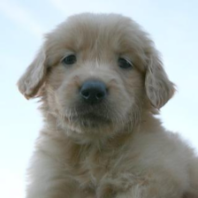
\includegraphics[width=0.25\textwidth]{figure/varsaliency/varsaliency0.png}};
    \node[SIR, label={[align=center]Image without dog\\present, wrongly\\classified as "Dingo"}] (oodimg) [right=of idimg] {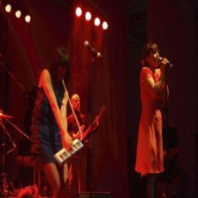
\includegraphics[width=0.25\textwidth]{figure/varsaliency/varsaliency2.png}};

    \node[SIR] (idsal) [below=1.5cm of idimg] {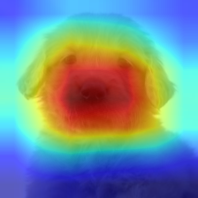
\includegraphics[width=0.25\textwidth]{figure/varsaliency/varsaliency1.png}};
    \node[SIR] (oodsal) [below=1.5cm of oodimg] {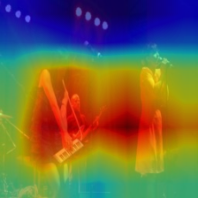
\includegraphics[width=0.25\textwidth]{figure/varsaliency/varsaliency3.png}};

    \node[SIR] (idmean) [below=1.5cm of idsal] {GINI = $0.6$};
    \node[SIR] (oodmean) [below=1.5cm of oodsal] {GINI = $0.2$};

    \draw[->, very thick] (idimg.south)  to node[midway, fill=white, align=center] {Generate \ac{xai} heatmap\\of model prediction} (idsal.north);
    \draw[->, very thick] (oodimg.south)  to node[midway, fill=white, align=center] {Generate \ac{xai} heatmap\\of model prediction} (oodsal.north);

    \draw[->, very thick] (idsal.south)  to node[midway, fill=white, align=center] {Calculate variance\\of normalized heatmap} (idmean.north);
    \draw[->, very thick] (oodsal.south)  to node[midway, fill=white, align=center] {Calculate variance\\of normalized heatmap} (oodmean.north);

    \node[SIR, align=left, draw=id, fill=id!30] (iddecision) [below=of idmean] {Above threshold:\\classified as \ac{id}};
    \node[SIR, align=left, draw=far, fill=far!30] (ooddecision) [below=of oodmean] {Below threshold:\\classified as \ac{ood}};

    \draw[->, very thick] (idmean.south)  to node[midway, fill=white] {Compare with threshold} (iddecision.north);
    \draw[->, very thick] (oodmean.south)  to node[midway, fill=white] {Compare with threshold} (ooddecision.north);

    \begin{scope}[shift={($(oodsal.east)+(0.1cm,0.25\textwidth / 2)$)}]
        \pgfplotscolorbardrawstandalone[
        colormap name=turbo,
        point meta min=0,
        point meta max=1,
        colorbar style={
            height=0.25\textwidth, % Match the height of the images
            width=0.4cm, % Desired width of the colorbar
            ytick={0, 0.5, 1},
            % yticklabels={Low, Medium, High},
        }]
    \end{scope}

    \end{tikzpicture}

    \caption[Spread of Saliency visual explanation]{Figure showing the functioning of the Spread of Saliency \ac{ood} detector in a hypothetical scenario where a model trained on images of dogs is shown an image with no dogs present. The heatmaps are here based on the normalized values of each saliency map, meaning that magnitude information is ignored}
    \label{fig:varsaliency}
    \end{center}
\end{figure}

\subsubsection{Proof that a special case of Saliency Aggregation is equivalent to the \acf{mls} \ac{ood} detector}

Finally, to further prove that the Saliency Aggregation framework can be used for \ac{ood} detection, I present a special case in which the \ac{ood} score outputted by a saliency aggregator is equivalent to \ac{mls}, one of the baseline methods used for \ac{ood} detection. The \ac{mls} \ac{ood} detector simply uses the maximum logit as an indicator of \ac{ood}-ness, and is described in more detail in section \ref{section:background_baselines}.

In this case, we use mean aggregation, and \ac{gradcam} as the saliency mapping method. In addition, we assume that the classification stage of the \ac{cnn} is a simple \ac{gap} over the feature map followed by a single linear layer. This is not an unreasonable assumption, as this is the classification head of all ResNet models. In addition, we perform \ac{gradcam} on the final layer of the network, which is recommended by \cite{gradcam}.

Following \cite{gradcam}, the saliency map has the following definition:

\begin{equation}
    L^c_{\text{GradCAM}} = ReLU\left(\sum_k \left( \frac{1}{N \cdot M} \sum_i \sum_j \frac{\delta y^c}{\delta A_{ij}^k} \right) A^k \right).
\end{equation}

Here, $A^k$ is the k'th channel of the final convolutional feature map, while $N$ and $M$ are its dimensions. The above equation simply describes averaging the gradients of the logit of class $c$ for each channel, and using these values to perform a weighted sum of the channels in the feature map, as described in section \ref{section:xaimethodsbackground}. As will be explained in more detail later, we do not wish to perform ReLU rectification with any of our saliency mapping methods, as we wish to keep all information extracted by the saliency mapping, not just the values which increase the probability of the predicted class. Using mean as the aggregation, the \ac{ood} score is then:

\begin{equation}
    \text{SalAgg}^c = \text{mean} \left(\sum_k \left( \frac{1}{N \cdot M} \sum_i \sum_j \frac{\delta y^c}{\delta A_{ij}^k} \right) A^k \right).
\end{equation}

For the given network, the logit $y^c$ for class $c$ is calculated in the following manner:

\begin{equation} \label{eq:quick}
    y^c = \sum_k \text{mean}(A_k) \cdot W_{ck} = \sum_k \left( \frac{\sum_i \sum_j A^k_{ij} \cdot W_{ck} }{N \cdot M}  \right) .
\end{equation}

This equation simply describes \ac{gap} (all channels are averaged to a single number) followed by a single linear layer (each logit is a weighted sum of the average pooled channels, with the weights defined by a specific row/column in the weight matrix $W$. To prove that Saliency Aggregation is equivalent to \ac{mls} \ac{ood} detection, we must simply prove that $\text{SalAgg}^c = y^c \cdot h$, where $h$ is some constant factor. We return to the equation for $\text{SalAgg}^c$:

\begin{equation} \label{eq:salagg}
    \text{SalAgg}^c = \text{mean} \left(\sum_k \left( \frac{1}{N \cdot M} \sum_i \sum_j \frac{\delta y^c}{\delta A_{ij}^k} \right) A^k \right).
\end{equation}

Given equation \ref{eq:quick},

\begin{equation}
    \frac{\delta y^c}{\delta A^k_{ij}} = \frac{W_{ck}}{N \cdot M}.
\end{equation}

As we can see, the indices $i$ and $j$ have disappeared. This is to be expected, as global average pooling means that all values in each channel are multiplied by the same value when calculating the logits. We may now substitute this derivative in the equation \ref{eq:salagg}:

\begin{equation}
    \text{SalAgg}^c = \text{mean} \left(\sum_k \left( \frac{1}{N \cdot M} \sum_i \sum_j \frac{W_{ck}}{N \cdot M} \right) A^k \right).
\end{equation}

We now reorder the terms somewhat:

\begin{gather}
    \text{SalAgg}^c = \text{mean} \left(\sum_k \left( \frac{1}{N \cdot M} \sum_i \sum_j \frac{W_{ck}}{N \cdot M} \right) A^k \right) \\
    = \frac{1}{N \cdot M} \text{mean} \left(\sum_k \left( \frac{1}{N \cdot M} \sum_i \sum_j W_{ck} \right) A^k \right) \\
    = \frac{1}{N \cdot M} \text{mean} \left(\sum_k \left( \frac{1}{N \cdot M} (N \cdot M) W_{ck} \right) A^k \right) \\
    = \frac{1}{N \cdot M} \text{mean} \left(\sum_k  W_{ck} \cdot A^k \right)
\end{gather}

We know that $\text{mean}(aX + bY) = a \cdot \text{mean}(X) + b \cdot \text{mean}(Y)$, allowing the following:

\begin{equation}
    \text{SalAgg}^c = \frac{1}{N \cdot M} \sum_k  W_{ck} \cdot \text{mean}(A^k).
\end{equation}

We recognize the summation above as $y^c$ as described in equation \ref{eq:quick}. If denote $1 / (N \cdot M)$ as $h$, we have

\begin{equation}
    \text{SalAgg}^c = h \cdot y^c,
\end{equation}

which was what we wanted to prove. Choosing $c$ as $\max_i y^i$, the right hand side is the \ac{mls} \ac{ood} score multiplied by a constant factor, while the left hand side is the mean value of the \ac{gradcam} saliency map generated from the predicted class. The constant factor has no effect on the \ac{ood} detection, as it just means that the threshold on \ac{mls} will be scaled down compared to Saliency Aggregation in this case, with all predictions being the same for either method. We have now shown that \ac{xai} saliency mapping methods, although they are made for an entirely different purpose than \ac{ood} detection, also collect information from the network which can be used for \ac{ood} detection.

\subsubsection{Saliency Aggregation \ac{ood} detector: formal definition}

With the both the intuition and the mathematical justification explained, we may now formalize the method. To define this detector mathematically, let us first define the necessary components. As in chapter \ref{chapter:background}, we assume we have a model $f: \bm{x} \to \R^C$. In this case, $\bm{x} \in \R^{D \times H \times W}$, i.e a $D$ channel image of height $H$ and width $W$. In addition, we define a \ac{xai} saliency mapping method $s: (f, \bm{x}) \to \R^{H_s \times W_s}$. This function takes the model $f$ and an input $\bm{x}$ and returns a $H_s$ by $W_s$ saliency map for the predicted class, i.e. the class corresponding to the highest logit. We also define an aggregation function $A: \bm{x} \rightarrow \R$, where $\bm{x}$ can be of any shape. Given the fact that we do not know whether the saliency aggregation of a specific \ac{xai} method $s$ and a specific model $f$ will be larger or smaller for \ac{id} data, we must also decide whether larger or smaller values should be considered \ac{id}. To do this, we can calculate the mean value of the \ac{ood} detector over a validation \ac{id} and validation \ac{ood} dataset, and compare their values. Requiring the presence of a validation set does not impose any actual limitations on the method, as a validation set is required for all \ac{ood} detection methods, to be able to set the threshold $\delta$. If we denote the mean value of the aggregation over the \ac{id} validation dataset as $\mu_{id}$, and over the \ac{ood} dataset as $\mu_{ood}$, we can use $\text{sign}(\mu_{id} - \mu_{ood})$ to multiply the \ac{ood} detection score by $1$ or $-1$, respectively. This ensures that the \ac{ood} detector follows the convention of the \ac{ood} detection field, which is that \ac{id} samples should have higher scores than \ac{ood} samples on a given \ac{ood} detection metric.

Thus, the \ac{ood} detector has the following form, given a threshold $\delta$:

\begin{align}
    g(\bm{x}; s, A, \delta)=\begin{cases} 
        \text{in } & \text{sign}(\mu_{id} - \mu_{ood}) \cdot A(s(\bm{x}, f)) \ge \delta \\
        \text{out} & \text{sign}(\mu_{id} - \mu_{ood}) \cdot A(s(\bm{x}, f)) < \delta 
   \end{cases}
\label{eq:aggregate}
\end{align}

An astute reader may note that aggregation functions are permutation invariant, meaning that all positional information from the two-dimensional saliency maps is lost when aggregating. This may seem strange, as it is primarily the positions of the different values that is important when using \ac{xai} methods for explaining model predictions on images. However, there is good reason to believe that for many image classification tasks, the positions of the points of interest in an \ac{xai} saliency map does not carry much discriminative potential. For datasets such as CIFAR10 and ImageNet200, there is a huge variety in the positions of the ground truth class (a dog may appear in the middle, the top right corner, or any other position and still be of the class 'dog'). As such, it is not a given that the removal of positional information will be massively detrimental. In fact, when \cite{martinez} reflects upon the poor results of their saliency heatmap clustering for detecting \ac{ood} samples on CIFAR10, it is exactly this variability in position they highlight: "Indeed, the CIFAR10-C dataset does not afford the positional bias and low intra-class variability observed in the previous case studies: informative objects for the classes to be predicted appear in arbitrary parts of the image and have a high degree of compositional variability".

Given the exploratory nature of this thesis, it is reasonable to try many different forms of aggregation. Even when just considering the magnitude, it would be insufficient to just use the mean or maximum value of each saliency map, as each form of aggregation captures different qualities about the underlying data. The maximum value, for example, is sensitive to outliers, which may be detrimental. The median value is far less sensitive to outliers, but given that one might expect \ac{id} data to have regions which are very important while most regions are relatively unimportant, this metric may not capture these high values. The vector norm and range are invariant to the sign of the saliencies, which means that if there are both large positive and negative values, these aggregates will return large scores. This is in contrast to the mean, median and third quartile, which will be lower if there are many negative values. In summary, we do not have the prerequisite knowledge about the distribution of saliency maps on \ac{id} and \ac{ood} data to make an informed selection, and as such we should cast a wide net when choosing which forms of aggregation to use.

In the experiments, the following aggregations have been used. \\


% \begin{center}
% \begin{table}[h]
%     \centering
%     \begin{tabular}{|c|c|}
%     \hline
%     Aggregation & Description \\
%     \hline
%     \multicolumn{2}{|c|}{\textbf{Magnitude}} \\
%     \hline
%     Mean & \\
%     Median & \\
%     Vector norm & \\
%     Range & \\
%     Maximum & \\
%     Third Quartile & \\
%     \hline
%     \multicolumn{2}{|c|}{\textbf{Statistical Dispersion}} \\
%     \hline
%     \acs{cv} & \\
%     \acs{qcd} & \\
%     \acs{rmd} & \\
%     \hline
%     \end{tabular}
%     \caption{Descriptor types}
% \end{table}
% \end{center}

\textbf{Magnitude:}
\begin{itemize}
    \itemsep0em
    \item Mean
    \item Median
    \item Vector norm
    \item Range
    \item Maximum
    \item Third Quartile
\end{itemize}

\textbf{Statistical dispersion:}
\begin{itemize}
    \itemsep0em
    \item \acf{cv}
    \item \acf{qcd}
    \item \acf{rmd}
\end{itemize}

These two categories follow the intuition explained above, and will test whether either the magnitude or statistical spread of \ac{id} saliency maps differ substantially from those of \ac{ood} saliency maps.

% The magnitude based aggregations are essentially self-explanatory. For the distribution based methods, some explanation is necessary. The \acf{cv} is an alternative to using standard deviation, which removes the effect of the magnitude of the values over which the standard deviation is calculated. The \ac{cv} of a set of values is simply the standard deviation divided by the mean: $CV(\mathbf{x}) = \sigma_x / \mu_x$. For exploring whether the saliencies of \ac{ood} data is more dispersed or spread out than \ac{id} data, such a normalization is required, given that we do not expect the saliencies of \ac{id} and \ac{ood} data to have the same magnitude. Skewness is a measure of asymmetry of a distribution, and can tell us something about the outliers of the saliency maps and their location in relation to the rest of the values. The Gini coefficient is another measure of statistical dispersion, most commonly used to measure income and wealth inequality. The Gini-coefficient of a data set where all values are the same is zero, while it is 1 for a data set where all values are 0 except for one. 

\subsection{Saliency integrated into existing \ac{ood} detection algorithms}

Given the poor results of \cite{martinez}, one might expect that saliency maps on their own are insufficient to differentiate \ac{id} and \ac{ood} data. \cite{combood} has shown that by combining the \ac{ood} detection scores of two different methods, the total performance can be improved considerably. Furthermore, \cite{vim} has shown improvements by considering the softmax, logit and feature space in tandem. Thus, there is reason to believe that if \ac{xai} saliency maps have some discriminatory capabilities, these could be combined with traditional method \ac{ood}, resulting in a performance gain. As such, I further present two methods which use both saliencies and traditional \ac{ood} detection metrics, to investigate if the addition of saliency values can enhance existing methods.

\subsubsection{Maximum Logit + Saliency Aggregate} \label{section:salpluslogitmethod}

In 2024, \cite{combood} introduced \texttt{COMBOOD}. This \ac{ood} detector combines the \ac{ood} detection scores of two different distance metrics; Mahalanobis distance and nearest neighbour distance. Each distance metric uses a different feature extraction method, which allows the two methods to collect different forms of information and complement each other. The combination is done by a simple unweighted addition of the confidence scores computed from the log distributions of the two metrics. \texttt{COMBOOD} achieves \ac{sota} performance, and is (at the time of writing) by far the best performing method on ImageNet200 in the OpenOOD benchmark. Based on these results, I propose a similar method for combining \ac{xai}-based and traditional \ac{ood} detection metrics. If it is the case that \ac{xai} methods extract \ac{ood} information from the model in ways which are substantially different from traditional \ac{ood} detection strategies, we may see improvements similar to those observed by \cite{combood}.

For this method, the \ac{ood} score is a sum of the maximum logit and a saliency aggregate. However, due to the fact that both the logit and saliency values can be of any arbitrary magnitude, we must normalize them before summing if we want each part to contribute equally to the final score. Thus, we can sum the Z-scores of each metric instead. This ensures that the values of the maximum logit and the saliency aggregate are distributed in about the same way. To calculate the Z-scores, we can simply subtract the mean and divide by the standard deviation over an entire \ac{id} validation dataset, for each metric. Thus, we calculate the mean and standard deviations of the max logit over an \ac{id} validation set $\mu_{\text{MLS}}^{id}$ and $\sigma_{\text{MLS}}^{id}$, as well as the mean and standard deviation of the aggregate of saliencies $\mu_{\text{Agg}}^{id}$ and $\sigma_{\text{Agg}}^{id}$. In addition, we must calculate the mean value of the aggregation metric over a validation \ac{ood} dataset, as we do not know whether a given aggregation is higher or lower for \ac{id} data. We denote this value as $\mu_{\text{Agg}}^{ood}$. We now have the necessary values required to define this method mathematically:

As in the previous section, we assume we have a model $f: \bm{x} \to \R^C$, an \ac{xai} saliency mapping method $s: (f, \bm{x}) \to \R^{H_s \times W_s}$, and an aggregation function $A: \bm{x} \rightarrow \R$. Let us denote $\text{sign}(\mu_{\text{Agg}}^{id} - \mu_{\text{Agg}}^{ood})$ as $S$, for readability. The \ac{ood} detector then has the following form, given a threshold $\delta$:

{\large
\begin{align}
    g(\bm{x}; s, A, \delta)=\begin{cases} 
    \text{in } &  S \cdot \frac{A(s(\bm{x}, f)) - \mu_{\text{Agg}}^{id}}{\sigma_{\text{Agg}}^{id}} + \frac{\max_i S(\bm{x}) - \mu_{\text{MLS}}^{id}}{\sigma_{\text{MLS}}^{id}} \ge \delta \\[10pt]
    \text{out} &  S \cdot \frac{A(s(\bm{x}, f)) - \mu_{\text{Agg}}^{id}}{\sigma_{\text{Agg}}^{id}} + \frac{\max_i S(\bm{x}) - \mu_{\text{MLS}}^{id}}{\sigma_{\text{MLS}}^{id}} < \delta \\
   \end{cases}
\label{eq:aggregate}
\end{align}
}

In fact, this detector can be simplified somewhat. Consider the following:

\begin{gather}
S \cdot \frac{A(s(\bm{x}, f)) - \mu_{\text{Agg}}^{id}}{\sigma_{\text{Agg}}^{id}} + \frac{\max_i S(\bm{x}) - \mu_{\text{MLS}}^{id}}{\sigma_{\text{MLS}}^{id}} = \\
S \left( \cdot \frac{A(s(\bm{x}, f))}{\sigma_{\text{Agg}}^{id}} - \frac{\mu_{\text{Agg}}^{id}}{\sigma_{\text{Agg}}^{id}} \right) + \frac{\max_i S(\bm{x})}{\sigma_{\text{MLS}}^{id}} - \frac{\mu_{\text{MLS}}^{id}}{\sigma_{\text{MLS}}^{id}} = \\
S \cdot \frac{A(s(\bm{x}, f))}{\sigma_{\text{Agg}}^{id}} + \frac{\max_i S(\bm{x})}{\sigma_{\text{MLS}}^{id}} - \left(S \cdot \frac{\mu_{\text{Agg}}^{id}}{\sigma_{\text{Agg}}^{id}} + \frac{\mu_{\text{MLS}}^{id}}{\sigma_{\text{MLS}}^{id}} \right)
\end{gather}

Notice how all the values in the third term of the above summation are constants; they do not depend on $\bm{x}$. Thus, we can disregard these terms, as all they do is shift all outputs by a constant value. The final \ac{ood} detector thus has the following form:

{\large
\begin{align}
    g(\bm{x}; s, A, \delta)=\begin{cases} 
    \text{in } &  S \cdot \frac{A(s(\bm{x}, f))}{\sigma_{\text{Agg}}^{id}} + \frac{\max_i S(\bm{x})}{\sigma_{\text{MLS}}^{id}} \ge \delta \\[10pt]
    \text{out} &  S \cdot \frac{A(s(\bm{x}, f))}{\sigma_{\text{Agg}}^{id}} + \frac{\max_i S(\bm{x})}{\sigma_{\text{MLS}}^{id}} < \delta \\[10pt]
   \end{cases}
\label{eq:aggregate}
\end{align}
}

\subsubsection{SaliencyVIM: Virtual Logit Matching with Saliencies} \label{section:saliencyvim_method}

As a final proof-of-concept method, I propose adding saliency values directly into preexisting \ac{ood} detection models. For this, \ac{vim} \cite{vim} is a fitting choice, as \ac{vim} attempts to combine information from different sources, namely from the feature, logit and softmax probability space. As we can recall from section \ref{section:vim}, \ac{vim} uses a "virtual logit" which is calculated from the output features on the penultimate layer and appended to the original logits. As a proof-of-concept integration of saliencies into this method, we may append \ac{xai} saliencies to the features prior to the generation of this virtual logit. The virtual logit in \ac{vim} is calculated as the information lost when performing a \ac{pca} feature reduction on the features. By appending the saliencies, the \ac{pca} takes into account not just how the penultimate features vary together, but also the interplay between the penultimate features and the \ac{xai} saliencies, which may be substantially different between \ac{id} and \ac{ood} datasets. This increase in variance could increase the reconstruction loss when projecting \ac{ood} samples using the principal components calculated from the \ac{id} dataset, increasing the separability of \ac{id} and \ac{ood} data points. Because there is no equivalent to centering the feature space as described in \cite{vim} for saliencies, I keep the saliencies as they are while the features are centered.

To define this \ac{ood} detector mathematically, we follow the definition of \cite{vim} very closely. We assume we have a model $f: \bm{x} \to \R^C$ and a \ac{xai} saliency mapping method $s: (f, \bm{x}) \to \R^{H_s \times W_s}$. We further assume we can extract the penultimate features $h \in \R^K$, with a function $g: (f, \bm{x}) \to \R^K$. We denote these extracted features as $\bm{z}$, and the entire set of feature vectors over the \ac{id} dataset as $Z \in \R^{N \times K}$. As in \cite{vim}, we calculate an offset $\bm{o} = -(W^T)^+\bm{b}$, where $W$ and $\bm{b}$ are the weights and biases which transform the features into logits. The feature matrix $Z$ is transformed by this offset: $Z^\dagger = Z + \bm{o}$. In addition to this feature matrix, we also calculate saliencies over the \ac{id} dataset, and flatten them to produce a saliency matrix $S \in \R^{N \times (H_s \cdot W_s)}$. These two matrices are concatenated, giving us the matrix $Y = \left[ Z^\dagger, S \right]$. We then perform and eigendecomposition on $Y^TY$, as part of the \ac{pca} and in accordance with the method described by \cite{vim}:

\begin{equation}
    Y^TY = Q\Lambda Q^{-1}
\end{equation}

The first $D$ columns of $Q$ make up the $D$-dimensional principal subspace $P$. $D$ is a hyperparameter that must be tuned, and is usually some fraction of $K$, the amount of logits in the penultimate layer (for example, if the number of logits is 1024, $D$ may be 512 or 256). For this thesis, $D$ has been fixed at 256, to avoid the extra computational overhead required for hyperparameter tuning. Regardless of the value of $D$, the remaining $K - D$ columns make up the null-space of $P$. We denote matrix making up these remaining columns as $R$. With this matrix, we can calculate the residual of $\bm{x}$ onto $P$ as $\bm{x}^{P^T} = RR^T\bm{x}$. The virtual logit then has the following form:

\begin{equation}
l_0 := \alpha || \bm{x}^{\text{Null}(P)}|| = \alpha \sqrt{\bm{x}^T RR^T\bm{x}}
\end{equation}

This is exactly the same as the virtual logit for \ac{vim}, with the only difference being that $R$ is calculated from the concatenated matrix $Y$, which includes both saliencies and logits, as opposed to only logits. To make it clear that $R$ no longer depends solely on the network $f$ and the input data, but also on the choice of saliency generator $s$, we can denote $R$ as $R_s$. As with \ac{vim}, $\alpha$ is calculated from the average virtual and maximum logit over the \ac{id} dataset before the \ac{ood} detector is put into use.

The \ac{ood} detection score is the softmax score of the virtual logit when appended to the rest of the logits:

\begin{equation}
\text{SaliencyVIM}(\bm{x}) = \frac{e^{\alpha\sqrt{\bm{x}^TR_sR_s^T\bm{x}}}}{\sum_{i=1}^C e^{l_i} + e^{\alpha\sqrt{\bm{x}^TR_sR_s^T\bm{x}}}}
\end{equation}

Thus, the formal definition of the SaliencyVIM \ac{ood} detector is as follows, given a threshold $\delta$:

\begin{align}
    g(\bm{x}; \delta)=\begin{cases} 
        \text{in } & \text{SaliencyVIM}(\bm{x}) \ge \delta \\[10pt]
        \text{out} & \text{SaliencyVIM}(\bm{x}) < \delta \\[10pt]
   \end{cases}
\label{eq:aggregate}
\end{align}

Because we are no longer aggregating the saliencies, the choice of saliency method is no longer as free as with the previous two methods. When we wish to use the saliencies directly, we cannot use methods which output one value for every single pixel in the input image, as this would lead tens of thousands of dimensions over which to compute a \acf{pca}. This is computationally intractable. Instead, we must use methods which calculate saliencies over larger windows, such as occlusion, \ac{lime} or \ac{gradcam}.


\section{Benchmarks} \label{section:benchmarks}

After having introduced the three novel \ac{ood} detection methods that I plan to test, I will now introduce the \ac{ood} detection benchmarks that will be used. To best align this thesis with the broader \ac{ood} detection field, I will use the OpenOOD framework, and their collection of \ac{id} and \ac{ood} datasets. Each \ac{ood} detection benchmark is defined by an \ac{id} dataset, and a selection of corresponding \ac{ood} datasets. As described in \cite{openood15}, the four standard \ac{ood} detection benchmarks included in OpenOOD are CIFAR10, CIFAR100, ImageNet200, and ImageNet1K. I have used all four benchmarks in this thesis, to ensure that the results are robust and easily comparable to the \ac{sota} within the field of \ac{ood} detection.

\subsection{CIFAR10/CIFAR100}

CIFAR10 and CIFAR100 are two general object recognition datasets collected by \cite{cifar}. These datasets are commonly used in \ac{ai} research \cite{pouyanfar2018survey}. Each RGB image has dimensions $32 \times 32$, and there are 50 000 training images and 10 000 test images for both datasets. In CIFAR10, each of the ten classes has 5000 training samples and 1000 test samples, while for CIFAR100 each of the one hundred classes has 500 training samples and 100 test samples. For CIFAR10, the ten classes are as follows: airplanes, cars, birds, cats, deer, dogs, frogs, horses, ships, and trucks. The classes in CIFAR100 is in the same vein, but without any overlap with CIFAR10. OpenOOD presents a series of Near-\ac{ood} and Far-\ac{ood} datasets which are used in conjunction with these datasets and constitute the benchmarks. Both datasets have the same Far-\ac{ood} datasets, and also use TinyImageNet for Near-\ac{ood} evaluation. In addition, the CIFAR10 benchmark uses CIFAR100 as a Near-\ac{ood} dataset, while the CIFAR100 benchmark uses CIFAR10. Table \ref{table:cifar10} presents a short description of each dataset in the benchmarks, as well as the number of samples in the set for each dataset.

\begin{table}[H]
\begin{center}
\begin{tabular}{ |c|c|l| } 
    \hline
    Dataset & Size & Description \\
    \hline
    \rowcolor{id!50}
    CIFAR10/CIFAR100 & 10 000 & General objects \\ 
    \hline
    \rowcolor{near!50}
    CIFAR100/CIFAR10 & 10 000 & General objects \\ 
    \rowcolor{near!50}
    TinyImageNet & 7 793 & General objects downsampled from ImageNet \\ 
    \hline
    \rowcolor{far!50}
    MNIST & 70 000 & Handwritten digits from 0 to 9 \\ 
    \rowcolor{far!50}
    SVHN & 26 032 & Street view house numbers \\ 
    \rowcolor{far!50}
    Texture & 5 640 & Textural patterns \\ 
    \rowcolor{far!50}
    Places365 & 35 195 & Places, scenes, locations \\ 
    \hline
    \end{tabular}
    \caption{Hello}
    \label{table:cifar10}
\end{center}
\end{table}

In addition, a sample of images from CIFAR10 and the corresponding \ac{ood} datasets are shown in figure \ref{fig:cifar10}. Given that the only difference between the CIFAR10 and CIFAR100 benchmark is that CIFAR10 becomes a Near-\ac{ood} dataset and CIFAR100 becomes the \ac{id} dataset, this figure will suffice to give an impression of both benchmarks.

\begin{figure}[H]
    \begin{center}
    \begin{tikzpicture}[
    SIR/.style={rectangle, draw=black!80, thick, minimum size=5mm},
    ]
    % Define the size of each image cell
    \def\cellwidth{2.3cm}
    \def\cellheight{2.3cm}
    \def\rowpadding{0.8cm}
    \pgfmathtruncatemacro{\offset}{\cellheight + \rowpadding}
    % Loop through the grid
    \foreach \row in {0, 1, 2, 3, 4, 5, 6} {
        \foreach \col in {0, 1, 2} {
            % Calculate the image number
            \pgfmathtruncatemacro{\imagenumber}{\row * 3 + \col}
            % Draw the image
            \node[inner sep=0] (\imagenumber) at (\col * \cellwidth, -\row * \offset - \cellheight) 
                {\includegraphics[width=\cellwidth, height=\cellheight]{figure/cifar10_examples/image-img\imagenumber.png}};
        }
    }
    \node [above=0.1cm of 1] {\ac{id}: CIFAR10};
    \node [above=0.1cm of 4] {Near-\ac{ood}: CIFAR100};
    \node [above=0.1cm of 7] {Near-\ac{ood}: TinyImageNet};
    \node [above=0.1cm of 10] {Far-\ac{ood}: MNIST};
    \node [above=0.1cm of 13] {Far-\ac{ood}: SVHN};
    \node [above=0.1cm of 16] {Far-\ac{ood}: Texture};
    \node [above=0.1cm of 19] {Far-\ac{ood}: Places365};
    \begin{scope}[on background layer={color=id!50}]
        \fill (-1.5,-0.4) rectangle (6.2,-3.6);
    \end{scope}
    \begin{scope}[on background layer={color=near!50}]
        \fill (-1.5,-3.6) rectangle (6.2,-9.8);
    \end{scope}
    \begin{scope}[on background layer={color=far!50}]
        \fill (-1.5,-9.8) rectangle (6.2,-22.3);
    \end{scope}
    \end{tikzpicture}
    \caption[CIFAR10 dataset example images]{Figure showing three example images from CIFAR10 and from the corresponding \ac{ood} datasets}
    \label{fig:cifar10}
    \end{center}
\end{figure}



\subsection{ImageNet200/ImageNet1K}

ImageNet is another ubiquitous image classification dataset, which is used in large majority of computer vision works. In contrast to CIFAR, ImageNet images are substantially larger, at $256 \times 256$\footnote{It is common to center crop as part of preprocessing on ImageNet, and as such you will more often see the dimensions $224 \times 224$ mentioned in this thesis}. This increase in dimensionality could be used to argue that ImageNet tasks are more realistic, as it is rare that one would use $32 \times 32$ images in practical applications. The ImageNet dataset contains 1000 classes of general objects. In addition, there exists smaller versions, such as ImageNet200. As with the other \ac{id} datasets, OpenOOD contains a selection of \ac{ood} datasets which are chosen to test a model's ability to differentiate between different forms of \ac{ood} data. These \ac{ood} datasets, along with the \ac{id} dataset, constitute the \ac{ood} detection benchmark. Here, OpenOOD does not use ImageNet200 as a Near-\ac{ood} dataset for ImageNet1K, nor vice versa.Instead, both datasets use exactly the same \ac{ood} datasets, to facilitate straight comparisons between the performance on ImageNet1K and ImageNet200 \cite{openood15}. Table \ref{table:imagenet200} lists these datasets, and gives a short description for each one.

\begin{table}
\begin{center}
\begin{tabular}{ |c|c|l| } 
    \hline
    Dataset & Size & Description \\
    \hline
    \rowcolor{id!50}
    ImageNet200/ImageNet1K & 45 000/9 000 & General objects \\ 
    \hline
    \rowcolor{near!50}
    SSB-Hard & 49 000 & General objects taken from ImageNet21K \\ 
    \rowcolor{near!50}
    NINCO & 5 879 & General objects, manually curated by \cite{bitterwolf2023ninco} \\ 
    \hline
    \rowcolor{far!50}
    iNaturalist & 10 000 & Various animals \\ 
    \rowcolor{far!50}
    Texture & 5 160 & Textural patterns \\ 
    \rowcolor{far!50}
    OpenImage-O & 15 869 & General objects, manually curated by \cite{vim} \\ 
    \hline
    \end{tabular}
    \caption{Hello}
    \label{table:imagenet200}
\end{center}
\end{table}

In addition, figure \ref{fig:imagenet200} shows three example images for each dataset in the ImageNet200 benchmark. Like the preceding section, I will not show a separate figure for ImageNet1K, as the only change would be the \ac{id} dataset, which would show slightly different classes.

\begin{figure}[H]
    \begin{center}
    \begin{tikzpicture}[
    SIR/.style={rectangle, draw=black!80, thick, minimum size=5mm},
    ]
    % Define the size of each image cell
    \def\cellwidth{2.3cm}
    \def\cellheight{2.3cm}
    \def\rowpadding{0.8cm}
    \pgfmathtruncatemacro{\offset}{\cellheight + \rowpadding}
    % Loop through the grid
    \foreach \row in {0, 1, 2, 3, 4, 5} {
        \foreach \col in {0, 1, 2} {
            % Calculate the image number
            \pgfmathtruncatemacro{\imagenumber}{\row * 3 + \col}
            % Draw the image
            \node[inner sep=0] (\imagenumber) at (\col * \cellwidth, -\row * \offset - \cellheight) 
                {\includegraphics[width=\cellwidth, height=\cellheight]{figure/imagenet200_examples/image-img\imagenumber.png}};
        }
    }
    \node [above=0.1cm of 1] {\ac{id}: ImageNet200};
    \node [above=0.1cm of 4] {Near-\ac{ood}: SSB-Hard};
    \node [above=0.1cm of 7] {Near-\ac{ood}: NINCO};
    \node [above=0.1cm of 10] {Far-\ac{ood}: iNaturalist};
    \node [above=0.1cm of 13] {Far-\ac{ood}: Texture};
    \node [above=0.1cm of 16] {Far-\ac{ood}: OpenImage-O};
    \begin{scope}[on background layer={color=id!50}]
        \fill (-1.5,-0.4) rectangle (6.2,-3.6);
    \end{scope}
    \begin{scope}[on background layer={color=near!50}]
        \fill (-1.5,-3.6) rectangle (6.2,-9.8);
    \end{scope}
    \begin{scope}[on background layer={color=far!50}]
        \fill (-1.5,-9.8) rectangle (6.2,-19.1);
    \end{scope}
    \end{tikzpicture}
    \caption[ImageNet200 dataset example images]{Figure showing three example images from ImageNet200 and from the corresponding \ac{ood} datasets}
    \label{fig:imagenet200}
    \end{center}
\end{figure}


\subsection{Overview of testing environment} \label{section:testing_environment}

After having introduced the specific benchmarks, I will describe the testing environment that has been used, so that it is clear for the reader how the \ac{ood} detection metrics are calculated.

As we have seen, for a given \ac{id} dataset, we have a series of \ac{ood} datasets, which are all semantically shifted in relation to the \ac{id} dataset. These \ac{ood} datasets are categorized into Near- and Far-\ac{ood}, depending on the degree of their semantic shift. The \ac{id} dataset is split into a train, validation and test set, while the \ac{ood} datasets are split into validation and test sets. A network is trained on the train \ac{id} set.  Then, one \ac{ood} validation set is chosen to be used for hyperparameter tuning. Any hyperparameters that the \ac{ood} detection algorithm may have are tuned on this validation set and the \ac{id} validation dataset. After having trained the network and tuned the \ac{ood} detector, we now have every part needed to perform \ac{ood} detection and calculate performance metrics.

First, we calculate \ac{ood} detection scores over the entire \ac{id} test set. By convention, these are expected to be higher than for \ac{ood} samples. For example, if we use the \ac{msp} \ac{ood} detector as described in section \ref{section:background_baselines}, we would calculate the softmax score of the predicted class for all samples in the \ac{id} test set and store them. Then, for each \ac{ood} test dataset, we perform the same calculation of \ac{ood} detection scores. To calculate \ac{auroc} and \ac{fpr95}, each set of \ac{ood} test set scores is compared against the \ac{id} test set scores we calculated previously by denoting all \ac{id} samples as class 0 and all \ac{ood} samples as class 1. After having done this for each \ac{ood} test set individually, we have a series of Near- and Far-\ac{ood} \ac{auroc} and \ac{fpr95} scores. The average performance of our classifier on Near- and Far-\ac{ood} can then be calculated by averaging over these individual scores. Figure \ref{fig:testing_environment} shows a diagram of this process.

TODO: FIGURE

This process describes how the performance of an \ac{ood} detector can be calculated for a given \ac{id} dataset and set of \ac{ood} datasets. However, when developing a new method, one cannot repeatedly perform this process on the same \ac{id} and \ac{ood} datasets, as this will bias then final results. A common option in such a scenario is to simply use some benchmarks for development and some for the final tests. However, in this case, this is not desirable. Firstly, to ensure comparisons with all methods tested under the OpenOOD framework, we should evaluate our performance on all benchmarks included within it. In addition, we have seen from the preceding section that the \ac{ood} datasets are shared between different \ac{id} benchmarks, which means that if we used the ImageNet200 benchmark as a development benchmark, we will have seen all \ac{ood} data of both ImageNet200 and ImageNet1K during development, which would disallow using ImageNet1K as a benchmark during testing.

Because of this, I have separated all benchmarks into validation and test benchmarks. Specifically, all \ac{id} and \ac{ood} validation sets, and all \ac{id} and \ac{ood} test sets have been split in two equally sized subsets, of which one half has been used during development and the other half has been used during the final testing. This has been done for all four benchmarks, ensuring that the results reported in chapter \ref{chapter:experiments} have not been biased by repeated testing on the same data. The development of new methods has been done on ImageNet200 and CIFAR10, as there is little benefit to using all four benchmarks during development. The final testing has been done on all benchmarks included in OpenOOD, as mentioned previously.

\section{Networks}

While it may be interesting to see how these new methods function on different network architectures, the combination of several different novel \ac{ood} detection algorithms and \ac{xai} saliency methods, as well as four different benchmarks, already presents a considerable amount of evaluation. Thus, to focus the thesis on comparing different \ac{ood} detection methods against each other, I believe it is best to fix other parameters such as network architecture. With this in mind, I choose to limit myself to the ResNet \cite{resnet} family of neural networks. In particular, I use ResNet18 for evaluation on CIFAR10, CIFAR100 and ImageNet200, and ResNet50 for evaluation on ImageNet1K. Given the scope of the of the thesis as described in section \ref{section:scope}, I do not use methods which require retraining of the network. As such, all networks are pretrained and I do not perform any training as part of this thesis.

Aside from \acp{cnn}, Vision Transformers also perform exceptionally on computer vision tasks, and achieve \ac{sota} results in many settings \cite{vit}. On ImageNet, they are even dominant, and the top 10 models when considering (top-1) accuracy are all based on vision transformers, as opposed to \acp{cnn}.\footnote{https://paperswithcode.com/sota/image-classification-on-imagenet} As such one might question the choice of a \ac{cnn} model, when newer and better models have been developed.

However, given that a large part of \ac{xai} methods have been developed under the \ac{cnn} paradigm, many \ac{xai} methods are not easily adapted to vision transformers. Methods such as \ac{gradcam} and \ac{lrp} exploit specific parts of \ac{cnn} architectures when generating explanations \cite{legrad}, and are thus difficult to use with different architectures. To be able to use a broad section of the representative \ac{xai} methods in use today, it is thus preferable to use \acp{cnn} as opposed to vision transformers.

\section{\ac{xai} Saliency Methods}

The theory of each \ac{xai} saliency method used in this thesis has been described in section \ref{section:xaimethodsbackground} of chapter \ref{chapter:background}. In the following section, I will describe the specifics of how I have applied each method in my efforts to better align them with the goal of separating \ac{id} and \ac{ood} data points.

For all saliency methods, one significant difference between my application and those commonly used for model explanation is that I modify all methods to return unnormalized and unrectified saliencies. For most \ac{xai} applications, it is common to rectify the saliencies such that negative saliencies are set to zero. In addition, some methods output normalized saliencies, as \ac{xai} saliency maps are intended to be inspected individually. In these cases, the absolute magnitude can be considered less relevant, and looking at saliencies relative to each other more informative. For my purposes, both negative values and the magnitude may convey important information which should not be discarded.

In addition any parameters of each \ac{xai} method has been fixed, and no hyperparameter tuning has been performed. Given that I have introduced three different \ac{xai} \ac{ood} detection frameworks which have been tested on four different benchmarks, tuning five \ac{xai} methods has been an additional computational burden that could not be afforded.

\subsection{\ac{lime}}

As is common when applying \ac{lime} to images, I have used segmentations of the input image to reduce the dimensionality of the input that is fed into the \ac{lime} algorithm. As explained in section \ref{section:saliencymapbackground}, superpixel segmentation algorithms such as \ac{slic} may increase the accuracy of the explanations, but are CPU-bound and thus introduce a considerable computational overhead (which is problematic when tens of thousands of samples are to be evaluated). Thus, I have chosen to stick to a simple rectangular segmentation instead. Each image is split into $N \times N$ equally sized rectangular regions, with $N$ being set to 4.

\subsection{Occlusion}

Like with \ac{lime}, I have used a rectangular segmentation approach, with each image being split into $N \times N$ regions. As with \ac{lime}, $N$ is set to 4, which ensures that accurate comparisons between \ac{lime} and occlusion can be made.

\subsection{\ac{gradcam}}

When utilizing \ac{gradcam}, a choice must be made about which convolutional layer one should calculate gradients from. As described in section \ref{section:cnn}, earlier layers have higher resolution (more precise spatial information) but lower field of view (less comprehensive semantic information) than later layers. In most cases, the final convolutional layer is seen as most informative, with \cite{gradcam} stating that "convolutional layers naturally retain spatial information which is lost in fully-connected layers, so we can expect the last convolutional layers to have the best compromise between high-level semantics and detailed spatial information". For this reason, I also use the final convolutional layer.

As mentioned previously, I do not apply any \ac{relu} activation function after calculating the saliencies, despite this being an explicit part of the methodology of \cite{gradcam}. This is because information about what the model regards as detrimental to the prediction may also be informative for \ac{ood} detection.

\subsection{Guided Backpropagation}

\ac{gbp} is a very simple method which is completely non-parametric, and as such no specific choices have had to be made. Like with all other methods, no normalization or rectification has been done to the output of \ac{gbp}.

\subsection{Integrated Gradients}

For integrated gradients, the only choice that must be made is the choice of baseline. An ideal baseline should convey no information, and should ideally lead to an output of zero from the network. As \cite{sturmfels2020visualizing} shows, there are no perfect choices for such a baseline, as all methods carry some assumption about our dataset and what it means for an input to "convey no information". However, the common choice for image classification tasks is the zero vector (a completely black image), as recommended by \cite{integratedgradients}. As such, this is the baseline I have used.

\section{Evaluation}

This section describes the details of how I have evaluated my methods on the four OpenOOD benchmarks.


\subsection{Metrics}

\ac{auroc} and \ac{fpr95} are the most common metrics used for \ac{ood} detection \cite{oodbaseline, odin, oodoverview, openood, vim}. In OpenOOD (\cite{openood}), \ac{auroc} is chosen as the primary metric used to rank methods against each other, as mentioned previously. As \cite{openood} by far presents the most comprehensive complete benchmark of all \ac{ood} detection methods to date, I have followed their methodology and used \ac{auroc} when evaluating my methods, while also calculating \ac{fpr95} as a secondary metric.

\ac{auroc} is agnostic to which class is the positive and which is the negative. Whether we consider \ac{ood} samples as 0 or 1, the result will be the same. However, the same is not true for \ac{fpr95}, necessitating a choice of positive and negative classes. There is no correct answer, but \cite{openood} chooses to consider \ac{ood} samples as the positive class, to "align with ML convention": It is common to consider abnormalities, anomalies, or the unexpected as the positive class (for example, a cancer detection system would consider the presence of cancer to be part of the positive class). This aligns with the goal of \ac{ood} detection, which is to detect abnormal inputs with regard to the data the model is trained on. Thus, I have also followed this convention and considered \ac{ood} samples as positive, and \ac{id} samples as negative. In this case, \ac{fpr95} has the following interpretation: "If a specific threshold leads to 95\% of \ac{ood} samples being correctly classified as \ac{ood}, what percentage of \ac{id} samples are then incorrectly classified as \ac{ood}"? In other words, \ac{fpr95} measures the rate of "false alarms" when 95\% of actual anomalies are caught.

For both of these metrics, the calculations are done on each \ac{ood} dataset individually, as opposed to comparing all \ac{ood} samples to the \ac{id} dataset. Afterwards, the metrics of all Near-\ac{ood} and Far-\ac{ood} are averaged, giving us two general performance metrics which tell us how a method functions on either Near-\ac{ood} or Far-\ac{ood}. This aligns with the methodology of \cite{openood}. Similarly, when plotting density plots for a given \ac{ood} detection metric, the densities of all Near- and all Far-\ac{ood} data points are combined, giving a more comprehensible overview than if all \ac{ood} data sets are individually. Figure \ref{fig:full_not_full} shows density plots before and after combining Near- and Far-\ac{ood}, on the maximum logit score of images from the CIFAR10 dataset. As we can see, there is not that much internal variance between the \ac{ood} datasets, allowing us to combine them without losing too much information.

\begin{figure}[H]
    \begin{center}
        %% Creator: Matplotlib, PGF backend
%%
%% To include the figure in your LaTeX document, write
%%   \input{<filename>.pgf}
%%
%% Make sure the required packages are loaded in your preamble
%%   \usepackage{pgf}
%%
%% Also ensure that all the required font packages are loaded; for instance,
%% the lmodern package is sometimes necessary when using math font.
%%   \usepackage{lmodern}
%%
%% Figures using additional raster images can only be included by \input if
%% they are in the same directory as the main LaTeX file. For loading figures
%% from other directories you can use the `import` package
%%   \usepackage{import}
%%
%% and then include the figures with
%%   \import{<path to file>}{<filename>.pgf}
%%
%% Matplotlib used the following preamble
%%   \def\mathdefault#1{#1}
%%   \everymath=\expandafter{\the\everymath\displaystyle}
%%   
%%   \ifdefined\pdftexversion\else  % non-pdftex case.
%%     \usepackage{fontspec}
%%   \fi
%%   \makeatletter\@ifpackageloaded{underscore}{}{\usepackage[strings]{underscore}}\makeatother
%%
\begingroup%
\makeatletter%
\begin{pgfpicture}%
\pgfpathrectangle{\pgfpointorigin}{\pgfqpoint{6.400000in}{4.800000in}}%
\pgfusepath{use as bounding box, clip}%
\begin{pgfscope}%
\pgfsetbuttcap%
\pgfsetmiterjoin%
\definecolor{currentfill}{rgb}{1.000000,1.000000,1.000000}%
\pgfsetfillcolor{currentfill}%
\pgfsetlinewidth{0.000000pt}%
\definecolor{currentstroke}{rgb}{1.000000,1.000000,1.000000}%
\pgfsetstrokecolor{currentstroke}%
\pgfsetdash{}{0pt}%
\pgfpathmoveto{\pgfqpoint{0.000000in}{0.000000in}}%
\pgfpathlineto{\pgfqpoint{6.400000in}{0.000000in}}%
\pgfpathlineto{\pgfqpoint{6.400000in}{4.800000in}}%
\pgfpathlineto{\pgfqpoint{0.000000in}{4.800000in}}%
\pgfpathlineto{\pgfqpoint{0.000000in}{0.000000in}}%
\pgfpathclose%
\pgfusepath{fill}%
\end{pgfscope}%
\begin{pgfscope}%
\pgfsetbuttcap%
\pgfsetmiterjoin%
\definecolor{currentfill}{rgb}{1.000000,1.000000,1.000000}%
\pgfsetfillcolor{currentfill}%
\pgfsetlinewidth{0.000000pt}%
\definecolor{currentstroke}{rgb}{0.000000,0.000000,0.000000}%
\pgfsetstrokecolor{currentstroke}%
\pgfsetstrokeopacity{0.000000}%
\pgfsetdash{}{0pt}%
\pgfpathmoveto{\pgfqpoint{0.800000in}{0.528000in}}%
\pgfpathlineto{\pgfqpoint{3.054545in}{0.528000in}}%
\pgfpathlineto{\pgfqpoint{3.054545in}{4.224000in}}%
\pgfpathlineto{\pgfqpoint{0.800000in}{4.224000in}}%
\pgfpathlineto{\pgfqpoint{0.800000in}{0.528000in}}%
\pgfpathclose%
\pgfusepath{fill}%
\end{pgfscope}%
\begin{pgfscope}%
\pgfsetbuttcap%
\pgfsetroundjoin%
\definecolor{currentfill}{rgb}{0.000000,0.000000,0.000000}%
\pgfsetfillcolor{currentfill}%
\pgfsetlinewidth{0.803000pt}%
\definecolor{currentstroke}{rgb}{0.000000,0.000000,0.000000}%
\pgfsetstrokecolor{currentstroke}%
\pgfsetdash{}{0pt}%
\pgfsys@defobject{currentmarker}{\pgfqpoint{0.000000in}{-0.048611in}}{\pgfqpoint{0.000000in}{0.000000in}}{%
\pgfpathmoveto{\pgfqpoint{0.000000in}{0.000000in}}%
\pgfpathlineto{\pgfqpoint{0.000000in}{-0.048611in}}%
\pgfusepath{stroke,fill}%
}%
\begin{pgfscope}%
\pgfsys@transformshift{0.994589in}{0.528000in}%
\pgfsys@useobject{currentmarker}{}%
\end{pgfscope}%
\end{pgfscope}%
\begin{pgfscope}%
\definecolor{textcolor}{rgb}{0.000000,0.000000,0.000000}%
\pgfsetstrokecolor{textcolor}%
\pgfsetfillcolor{textcolor}%
\pgftext[x=0.994589in,y=0.430778in,,top]{\color{textcolor}{\rmfamily\fontsize{10.000000}{12.000000}\selectfont\catcode`\^=\active\def^{\ifmmode\sp\else\^{}\fi}\catcode`\%=\active\def%{\%}$\mathdefault{0}$}}%
\end{pgfscope}%
\begin{pgfscope}%
\pgfsetbuttcap%
\pgfsetroundjoin%
\definecolor{currentfill}{rgb}{0.000000,0.000000,0.000000}%
\pgfsetfillcolor{currentfill}%
\pgfsetlinewidth{0.803000pt}%
\definecolor{currentstroke}{rgb}{0.000000,0.000000,0.000000}%
\pgfsetstrokecolor{currentstroke}%
\pgfsetdash{}{0pt}%
\pgfsys@defobject{currentmarker}{\pgfqpoint{0.000000in}{-0.048611in}}{\pgfqpoint{0.000000in}{0.000000in}}{%
\pgfpathmoveto{\pgfqpoint{0.000000in}{0.000000in}}%
\pgfpathlineto{\pgfqpoint{0.000000in}{-0.048611in}}%
\pgfusepath{stroke,fill}%
}%
\begin{pgfscope}%
\pgfsys@transformshift{1.619733in}{0.528000in}%
\pgfsys@useobject{currentmarker}{}%
\end{pgfscope}%
\end{pgfscope}%
\begin{pgfscope}%
\definecolor{textcolor}{rgb}{0.000000,0.000000,0.000000}%
\pgfsetstrokecolor{textcolor}%
\pgfsetfillcolor{textcolor}%
\pgftext[x=1.619733in,y=0.430778in,,top]{\color{textcolor}{\rmfamily\fontsize{10.000000}{12.000000}\selectfont\catcode`\^=\active\def^{\ifmmode\sp\else\^{}\fi}\catcode`\%=\active\def%{\%}$\mathdefault{5}$}}%
\end{pgfscope}%
\begin{pgfscope}%
\pgfsetbuttcap%
\pgfsetroundjoin%
\definecolor{currentfill}{rgb}{0.000000,0.000000,0.000000}%
\pgfsetfillcolor{currentfill}%
\pgfsetlinewidth{0.803000pt}%
\definecolor{currentstroke}{rgb}{0.000000,0.000000,0.000000}%
\pgfsetstrokecolor{currentstroke}%
\pgfsetdash{}{0pt}%
\pgfsys@defobject{currentmarker}{\pgfqpoint{0.000000in}{-0.048611in}}{\pgfqpoint{0.000000in}{0.000000in}}{%
\pgfpathmoveto{\pgfqpoint{0.000000in}{0.000000in}}%
\pgfpathlineto{\pgfqpoint{0.000000in}{-0.048611in}}%
\pgfusepath{stroke,fill}%
}%
\begin{pgfscope}%
\pgfsys@transformshift{2.244877in}{0.528000in}%
\pgfsys@useobject{currentmarker}{}%
\end{pgfscope}%
\end{pgfscope}%
\begin{pgfscope}%
\definecolor{textcolor}{rgb}{0.000000,0.000000,0.000000}%
\pgfsetstrokecolor{textcolor}%
\pgfsetfillcolor{textcolor}%
\pgftext[x=2.244877in,y=0.430778in,,top]{\color{textcolor}{\rmfamily\fontsize{10.000000}{12.000000}\selectfont\catcode`\^=\active\def^{\ifmmode\sp\else\^{}\fi}\catcode`\%=\active\def%{\%}$\mathdefault{10}$}}%
\end{pgfscope}%
\begin{pgfscope}%
\pgfsetbuttcap%
\pgfsetroundjoin%
\definecolor{currentfill}{rgb}{0.000000,0.000000,0.000000}%
\pgfsetfillcolor{currentfill}%
\pgfsetlinewidth{0.803000pt}%
\definecolor{currentstroke}{rgb}{0.000000,0.000000,0.000000}%
\pgfsetstrokecolor{currentstroke}%
\pgfsetdash{}{0pt}%
\pgfsys@defobject{currentmarker}{\pgfqpoint{0.000000in}{-0.048611in}}{\pgfqpoint{0.000000in}{0.000000in}}{%
\pgfpathmoveto{\pgfqpoint{0.000000in}{0.000000in}}%
\pgfpathlineto{\pgfqpoint{0.000000in}{-0.048611in}}%
\pgfusepath{stroke,fill}%
}%
\begin{pgfscope}%
\pgfsys@transformshift{2.870021in}{0.528000in}%
\pgfsys@useobject{currentmarker}{}%
\end{pgfscope}%
\end{pgfscope}%
\begin{pgfscope}%
\definecolor{textcolor}{rgb}{0.000000,0.000000,0.000000}%
\pgfsetstrokecolor{textcolor}%
\pgfsetfillcolor{textcolor}%
\pgftext[x=2.870021in,y=0.430778in,,top]{\color{textcolor}{\rmfamily\fontsize{10.000000}{12.000000}\selectfont\catcode`\^=\active\def^{\ifmmode\sp\else\^{}\fi}\catcode`\%=\active\def%{\%}$\mathdefault{15}$}}%
\end{pgfscope}%
\begin{pgfscope}%
\definecolor{textcolor}{rgb}{0.000000,0.000000,0.000000}%
\pgfsetstrokecolor{textcolor}%
\pgfsetfillcolor{textcolor}%
\pgftext[x=1.927273in,y=0.251766in,,top]{\color{textcolor}{\rmfamily\fontsize{10.000000}{12.000000}\selectfont\catcode`\^=\active\def^{\ifmmode\sp\else\^{}\fi}\catcode`\%=\active\def%{\%}Maximum Logit Score}}%
\end{pgfscope}%
\begin{pgfscope}%
\pgfsetbuttcap%
\pgfsetroundjoin%
\definecolor{currentfill}{rgb}{0.000000,0.000000,0.000000}%
\pgfsetfillcolor{currentfill}%
\pgfsetlinewidth{0.803000pt}%
\definecolor{currentstroke}{rgb}{0.000000,0.000000,0.000000}%
\pgfsetstrokecolor{currentstroke}%
\pgfsetdash{}{0pt}%
\pgfsys@defobject{currentmarker}{\pgfqpoint{-0.048611in}{0.000000in}}{\pgfqpoint{-0.000000in}{0.000000in}}{%
\pgfpathmoveto{\pgfqpoint{-0.000000in}{0.000000in}}%
\pgfpathlineto{\pgfqpoint{-0.048611in}{0.000000in}}%
\pgfusepath{stroke,fill}%
}%
\begin{pgfscope}%
\pgfsys@transformshift{0.800000in}{0.528000in}%
\pgfsys@useobject{currentmarker}{}%
\end{pgfscope}%
\end{pgfscope}%
\begin{pgfscope}%
\definecolor{textcolor}{rgb}{0.000000,0.000000,0.000000}%
\pgfsetstrokecolor{textcolor}%
\pgfsetfillcolor{textcolor}%
\pgftext[x=0.455863in, y=0.479775in, left, base]{\color{textcolor}{\rmfamily\fontsize{10.000000}{12.000000}\selectfont\catcode`\^=\active\def^{\ifmmode\sp\else\^{}\fi}\catcode`\%=\active\def%{\%}$\mathdefault{0.00}$}}%
\end{pgfscope}%
\begin{pgfscope}%
\pgfsetbuttcap%
\pgfsetroundjoin%
\definecolor{currentfill}{rgb}{0.000000,0.000000,0.000000}%
\pgfsetfillcolor{currentfill}%
\pgfsetlinewidth{0.803000pt}%
\definecolor{currentstroke}{rgb}{0.000000,0.000000,0.000000}%
\pgfsetstrokecolor{currentstroke}%
\pgfsetdash{}{0pt}%
\pgfsys@defobject{currentmarker}{\pgfqpoint{-0.048611in}{0.000000in}}{\pgfqpoint{-0.000000in}{0.000000in}}{%
\pgfpathmoveto{\pgfqpoint{-0.000000in}{0.000000in}}%
\pgfpathlineto{\pgfqpoint{-0.048611in}{0.000000in}}%
\pgfusepath{stroke,fill}%
}%
\begin{pgfscope}%
\pgfsys@transformshift{0.800000in}{1.003609in}%
\pgfsys@useobject{currentmarker}{}%
\end{pgfscope}%
\end{pgfscope}%
\begin{pgfscope}%
\definecolor{textcolor}{rgb}{0.000000,0.000000,0.000000}%
\pgfsetstrokecolor{textcolor}%
\pgfsetfillcolor{textcolor}%
\pgftext[x=0.455863in, y=0.955384in, left, base]{\color{textcolor}{\rmfamily\fontsize{10.000000}{12.000000}\selectfont\catcode`\^=\active\def^{\ifmmode\sp\else\^{}\fi}\catcode`\%=\active\def%{\%}$\mathdefault{0.05}$}}%
\end{pgfscope}%
\begin{pgfscope}%
\pgfsetbuttcap%
\pgfsetroundjoin%
\definecolor{currentfill}{rgb}{0.000000,0.000000,0.000000}%
\pgfsetfillcolor{currentfill}%
\pgfsetlinewidth{0.803000pt}%
\definecolor{currentstroke}{rgb}{0.000000,0.000000,0.000000}%
\pgfsetstrokecolor{currentstroke}%
\pgfsetdash{}{0pt}%
\pgfsys@defobject{currentmarker}{\pgfqpoint{-0.048611in}{0.000000in}}{\pgfqpoint{-0.000000in}{0.000000in}}{%
\pgfpathmoveto{\pgfqpoint{-0.000000in}{0.000000in}}%
\pgfpathlineto{\pgfqpoint{-0.048611in}{0.000000in}}%
\pgfusepath{stroke,fill}%
}%
\begin{pgfscope}%
\pgfsys@transformshift{0.800000in}{1.479218in}%
\pgfsys@useobject{currentmarker}{}%
\end{pgfscope}%
\end{pgfscope}%
\begin{pgfscope}%
\definecolor{textcolor}{rgb}{0.000000,0.000000,0.000000}%
\pgfsetstrokecolor{textcolor}%
\pgfsetfillcolor{textcolor}%
\pgftext[x=0.455863in, y=1.430993in, left, base]{\color{textcolor}{\rmfamily\fontsize{10.000000}{12.000000}\selectfont\catcode`\^=\active\def^{\ifmmode\sp\else\^{}\fi}\catcode`\%=\active\def%{\%}$\mathdefault{0.10}$}}%
\end{pgfscope}%
\begin{pgfscope}%
\pgfsetbuttcap%
\pgfsetroundjoin%
\definecolor{currentfill}{rgb}{0.000000,0.000000,0.000000}%
\pgfsetfillcolor{currentfill}%
\pgfsetlinewidth{0.803000pt}%
\definecolor{currentstroke}{rgb}{0.000000,0.000000,0.000000}%
\pgfsetstrokecolor{currentstroke}%
\pgfsetdash{}{0pt}%
\pgfsys@defobject{currentmarker}{\pgfqpoint{-0.048611in}{0.000000in}}{\pgfqpoint{-0.000000in}{0.000000in}}{%
\pgfpathmoveto{\pgfqpoint{-0.000000in}{0.000000in}}%
\pgfpathlineto{\pgfqpoint{-0.048611in}{0.000000in}}%
\pgfusepath{stroke,fill}%
}%
\begin{pgfscope}%
\pgfsys@transformshift{0.800000in}{1.954828in}%
\pgfsys@useobject{currentmarker}{}%
\end{pgfscope}%
\end{pgfscope}%
\begin{pgfscope}%
\definecolor{textcolor}{rgb}{0.000000,0.000000,0.000000}%
\pgfsetstrokecolor{textcolor}%
\pgfsetfillcolor{textcolor}%
\pgftext[x=0.455863in, y=1.906602in, left, base]{\color{textcolor}{\rmfamily\fontsize{10.000000}{12.000000}\selectfont\catcode`\^=\active\def^{\ifmmode\sp\else\^{}\fi}\catcode`\%=\active\def%{\%}$\mathdefault{0.15}$}}%
\end{pgfscope}%
\begin{pgfscope}%
\pgfsetbuttcap%
\pgfsetroundjoin%
\definecolor{currentfill}{rgb}{0.000000,0.000000,0.000000}%
\pgfsetfillcolor{currentfill}%
\pgfsetlinewidth{0.803000pt}%
\definecolor{currentstroke}{rgb}{0.000000,0.000000,0.000000}%
\pgfsetstrokecolor{currentstroke}%
\pgfsetdash{}{0pt}%
\pgfsys@defobject{currentmarker}{\pgfqpoint{-0.048611in}{0.000000in}}{\pgfqpoint{-0.000000in}{0.000000in}}{%
\pgfpathmoveto{\pgfqpoint{-0.000000in}{0.000000in}}%
\pgfpathlineto{\pgfqpoint{-0.048611in}{0.000000in}}%
\pgfusepath{stroke,fill}%
}%
\begin{pgfscope}%
\pgfsys@transformshift{0.800000in}{2.430437in}%
\pgfsys@useobject{currentmarker}{}%
\end{pgfscope}%
\end{pgfscope}%
\begin{pgfscope}%
\definecolor{textcolor}{rgb}{0.000000,0.000000,0.000000}%
\pgfsetstrokecolor{textcolor}%
\pgfsetfillcolor{textcolor}%
\pgftext[x=0.455863in, y=2.382212in, left, base]{\color{textcolor}{\rmfamily\fontsize{10.000000}{12.000000}\selectfont\catcode`\^=\active\def^{\ifmmode\sp\else\^{}\fi}\catcode`\%=\active\def%{\%}$\mathdefault{0.20}$}}%
\end{pgfscope}%
\begin{pgfscope}%
\pgfsetbuttcap%
\pgfsetroundjoin%
\definecolor{currentfill}{rgb}{0.000000,0.000000,0.000000}%
\pgfsetfillcolor{currentfill}%
\pgfsetlinewidth{0.803000pt}%
\definecolor{currentstroke}{rgb}{0.000000,0.000000,0.000000}%
\pgfsetstrokecolor{currentstroke}%
\pgfsetdash{}{0pt}%
\pgfsys@defobject{currentmarker}{\pgfqpoint{-0.048611in}{0.000000in}}{\pgfqpoint{-0.000000in}{0.000000in}}{%
\pgfpathmoveto{\pgfqpoint{-0.000000in}{0.000000in}}%
\pgfpathlineto{\pgfqpoint{-0.048611in}{0.000000in}}%
\pgfusepath{stroke,fill}%
}%
\begin{pgfscope}%
\pgfsys@transformshift{0.800000in}{2.906046in}%
\pgfsys@useobject{currentmarker}{}%
\end{pgfscope}%
\end{pgfscope}%
\begin{pgfscope}%
\definecolor{textcolor}{rgb}{0.000000,0.000000,0.000000}%
\pgfsetstrokecolor{textcolor}%
\pgfsetfillcolor{textcolor}%
\pgftext[x=0.455863in, y=2.857821in, left, base]{\color{textcolor}{\rmfamily\fontsize{10.000000}{12.000000}\selectfont\catcode`\^=\active\def^{\ifmmode\sp\else\^{}\fi}\catcode`\%=\active\def%{\%}$\mathdefault{0.25}$}}%
\end{pgfscope}%
\begin{pgfscope}%
\pgfsetbuttcap%
\pgfsetroundjoin%
\definecolor{currentfill}{rgb}{0.000000,0.000000,0.000000}%
\pgfsetfillcolor{currentfill}%
\pgfsetlinewidth{0.803000pt}%
\definecolor{currentstroke}{rgb}{0.000000,0.000000,0.000000}%
\pgfsetstrokecolor{currentstroke}%
\pgfsetdash{}{0pt}%
\pgfsys@defobject{currentmarker}{\pgfqpoint{-0.048611in}{0.000000in}}{\pgfqpoint{-0.000000in}{0.000000in}}{%
\pgfpathmoveto{\pgfqpoint{-0.000000in}{0.000000in}}%
\pgfpathlineto{\pgfqpoint{-0.048611in}{0.000000in}}%
\pgfusepath{stroke,fill}%
}%
\begin{pgfscope}%
\pgfsys@transformshift{0.800000in}{3.381655in}%
\pgfsys@useobject{currentmarker}{}%
\end{pgfscope}%
\end{pgfscope}%
\begin{pgfscope}%
\definecolor{textcolor}{rgb}{0.000000,0.000000,0.000000}%
\pgfsetstrokecolor{textcolor}%
\pgfsetfillcolor{textcolor}%
\pgftext[x=0.455863in, y=3.333430in, left, base]{\color{textcolor}{\rmfamily\fontsize{10.000000}{12.000000}\selectfont\catcode`\^=\active\def^{\ifmmode\sp\else\^{}\fi}\catcode`\%=\active\def%{\%}$\mathdefault{0.30}$}}%
\end{pgfscope}%
\begin{pgfscope}%
\pgfsetbuttcap%
\pgfsetroundjoin%
\definecolor{currentfill}{rgb}{0.000000,0.000000,0.000000}%
\pgfsetfillcolor{currentfill}%
\pgfsetlinewidth{0.803000pt}%
\definecolor{currentstroke}{rgb}{0.000000,0.000000,0.000000}%
\pgfsetstrokecolor{currentstroke}%
\pgfsetdash{}{0pt}%
\pgfsys@defobject{currentmarker}{\pgfqpoint{-0.048611in}{0.000000in}}{\pgfqpoint{-0.000000in}{0.000000in}}{%
\pgfpathmoveto{\pgfqpoint{-0.000000in}{0.000000in}}%
\pgfpathlineto{\pgfqpoint{-0.048611in}{0.000000in}}%
\pgfusepath{stroke,fill}%
}%
\begin{pgfscope}%
\pgfsys@transformshift{0.800000in}{3.857265in}%
\pgfsys@useobject{currentmarker}{}%
\end{pgfscope}%
\end{pgfscope}%
\begin{pgfscope}%
\definecolor{textcolor}{rgb}{0.000000,0.000000,0.000000}%
\pgfsetstrokecolor{textcolor}%
\pgfsetfillcolor{textcolor}%
\pgftext[x=0.455863in, y=3.809039in, left, base]{\color{textcolor}{\rmfamily\fontsize{10.000000}{12.000000}\selectfont\catcode`\^=\active\def^{\ifmmode\sp\else\^{}\fi}\catcode`\%=\active\def%{\%}$\mathdefault{0.35}$}}%
\end{pgfscope}%
\begin{pgfscope}%
\definecolor{textcolor}{rgb}{0.000000,0.000000,0.000000}%
\pgfsetstrokecolor{textcolor}%
\pgfsetfillcolor{textcolor}%
\pgftext[x=0.400308in,y=2.376000in,,bottom,rotate=90.000000]{\color{textcolor}{\rmfamily\fontsize{10.000000}{12.000000}\selectfont\catcode`\^=\active\def^{\ifmmode\sp\else\^{}\fi}\catcode`\%=\active\def%{\%}Density}}%
\end{pgfscope}%
\begin{pgfscope}%
\pgfpathrectangle{\pgfqpoint{0.800000in}{0.528000in}}{\pgfqpoint{2.254545in}{3.696000in}}%
\pgfusepath{clip}%
\pgfsetrectcap%
\pgfsetroundjoin%
\pgfsetlinewidth{2.007500pt}%
\definecolor{currentstroke}{rgb}{0.400000,0.760784,0.647059}%
\pgfsetstrokecolor{currentstroke}%
\pgfsetdash{}{0pt}%
\pgfpathmoveto{\pgfqpoint{1.156435in}{0.528027in}}%
\pgfpathlineto{\pgfqpoint{1.239031in}{0.529265in}}%
\pgfpathlineto{\pgfqpoint{1.280329in}{0.532216in}}%
\pgfpathlineto{\pgfqpoint{1.313367in}{0.536720in}}%
\pgfpathlineto{\pgfqpoint{1.338146in}{0.541811in}}%
\pgfpathlineto{\pgfqpoint{1.362924in}{0.548929in}}%
\pgfpathlineto{\pgfqpoint{1.387703in}{0.558635in}}%
\pgfpathlineto{\pgfqpoint{1.412482in}{0.571161in}}%
\pgfpathlineto{\pgfqpoint{1.445520in}{0.591228in}}%
\pgfpathlineto{\pgfqpoint{1.503337in}{0.626914in}}%
\pgfpathlineto{\pgfqpoint{1.536375in}{0.647660in}}%
\pgfpathlineto{\pgfqpoint{1.561154in}{0.666366in}}%
\pgfpathlineto{\pgfqpoint{1.585933in}{0.688209in}}%
\pgfpathlineto{\pgfqpoint{1.734605in}{0.828406in}}%
\pgfpathlineto{\pgfqpoint{1.751124in}{0.848699in}}%
\pgfpathlineto{\pgfqpoint{1.767643in}{0.873216in}}%
\pgfpathlineto{\pgfqpoint{1.784162in}{0.902630in}}%
\pgfpathlineto{\pgfqpoint{1.800682in}{0.936740in}}%
\pgfpathlineto{\pgfqpoint{1.825460in}{0.994424in}}%
\pgfpathlineto{\pgfqpoint{1.858499in}{1.078100in}}%
\pgfpathlineto{\pgfqpoint{1.883277in}{1.147641in}}%
\pgfpathlineto{\pgfqpoint{1.899796in}{1.201798in}}%
\pgfpathlineto{\pgfqpoint{1.916316in}{1.266768in}}%
\pgfpathlineto{\pgfqpoint{1.932835in}{1.347011in}}%
\pgfpathlineto{\pgfqpoint{1.949354in}{1.446953in}}%
\pgfpathlineto{\pgfqpoint{1.965873in}{1.570614in}}%
\pgfpathlineto{\pgfqpoint{1.982392in}{1.721301in}}%
\pgfpathlineto{\pgfqpoint{1.998911in}{1.901374in}}%
\pgfpathlineto{\pgfqpoint{2.015430in}{2.111909in}}%
\pgfpathlineto{\pgfqpoint{2.031950in}{2.352024in}}%
\pgfpathlineto{\pgfqpoint{2.056728in}{2.757667in}}%
\pgfpathlineto{\pgfqpoint{2.098026in}{3.458214in}}%
\pgfpathlineto{\pgfqpoint{2.114545in}{3.695690in}}%
\pgfpathlineto{\pgfqpoint{2.122805in}{3.795863in}}%
\pgfpathlineto{\pgfqpoint{2.131064in}{3.881080in}}%
\pgfpathlineto{\pgfqpoint{2.139324in}{3.949837in}}%
\pgfpathlineto{\pgfqpoint{2.147584in}{4.001009in}}%
\pgfpathlineto{\pgfqpoint{2.155843in}{4.033856in}}%
\pgfpathlineto{\pgfqpoint{2.164103in}{4.048000in}}%
\pgfpathlineto{\pgfqpoint{2.172362in}{4.043402in}}%
\pgfpathlineto{\pgfqpoint{2.180622in}{4.020327in}}%
\pgfpathlineto{\pgfqpoint{2.188881in}{3.979319in}}%
\pgfpathlineto{\pgfqpoint{2.197141in}{3.921172in}}%
\pgfpathlineto{\pgfqpoint{2.205401in}{3.846915in}}%
\pgfpathlineto{\pgfqpoint{2.213660in}{3.757789in}}%
\pgfpathlineto{\pgfqpoint{2.230179in}{3.540817in}}%
\pgfpathlineto{\pgfqpoint{2.246698in}{3.283422in}}%
\pgfpathlineto{\pgfqpoint{2.271477in}{2.853142in}}%
\pgfpathlineto{\pgfqpoint{2.312775in}{2.129048in}}%
\pgfpathlineto{\pgfqpoint{2.329294in}{1.867054in}}%
\pgfpathlineto{\pgfqpoint{2.345813in}{1.630895in}}%
\pgfpathlineto{\pgfqpoint{2.362332in}{1.423972in}}%
\pgfpathlineto{\pgfqpoint{2.378852in}{1.247449in}}%
\pgfpathlineto{\pgfqpoint{2.395371in}{1.100518in}}%
\pgfpathlineto{\pgfqpoint{2.411890in}{0.980825in}}%
\pgfpathlineto{\pgfqpoint{2.428409in}{0.885012in}}%
\pgfpathlineto{\pgfqpoint{2.444928in}{0.809276in}}%
\pgfpathlineto{\pgfqpoint{2.461447in}{0.749832in}}%
\pgfpathlineto{\pgfqpoint{2.477966in}{0.703232in}}%
\pgfpathlineto{\pgfqpoint{2.494486in}{0.666547in}}%
\pgfpathlineto{\pgfqpoint{2.511005in}{0.637451in}}%
\pgfpathlineto{\pgfqpoint{2.527524in}{0.614225in}}%
\pgfpathlineto{\pgfqpoint{2.544043in}{0.595676in}}%
\pgfpathlineto{\pgfqpoint{2.560562in}{0.580979in}}%
\pgfpathlineto{\pgfqpoint{2.577081in}{0.569484in}}%
\pgfpathlineto{\pgfqpoint{2.593600in}{0.560577in}}%
\pgfpathlineto{\pgfqpoint{2.618379in}{0.550704in}}%
\pgfpathlineto{\pgfqpoint{2.643158in}{0.543419in}}%
\pgfpathlineto{\pgfqpoint{2.676196in}{0.536117in}}%
\pgfpathlineto{\pgfqpoint{2.709234in}{0.531356in}}%
\pgfpathlineto{\pgfqpoint{2.742273in}{0.529018in}}%
\pgfpathlineto{\pgfqpoint{2.791830in}{0.528089in}}%
\pgfpathlineto{\pgfqpoint{2.800090in}{0.528055in}}%
\pgfpathlineto{\pgfqpoint{2.800090in}{0.528055in}}%
\pgfusepath{stroke}%
\end{pgfscope}%
\begin{pgfscope}%
\pgfpathrectangle{\pgfqpoint{0.800000in}{0.528000in}}{\pgfqpoint{2.254545in}{3.696000in}}%
\pgfusepath{clip}%
\pgfsetbuttcap%
\pgfsetroundjoin%
\pgfsetlinewidth{2.007500pt}%
\definecolor{currentstroke}{rgb}{0.552941,0.627451,0.796078}%
\pgfsetstrokecolor{currentstroke}%
\pgfsetdash{{7.400000pt}{3.200000pt}}{0.000000pt}%
\pgfpathmoveto{\pgfqpoint{0.927220in}{0.528032in}}%
\pgfpathlineto{\pgfqpoint{1.027309in}{0.529241in}}%
\pgfpathlineto{\pgfqpoint{1.063705in}{0.531549in}}%
\pgfpathlineto{\pgfqpoint{1.091002in}{0.535234in}}%
\pgfpathlineto{\pgfqpoint{1.109200in}{0.539257in}}%
\pgfpathlineto{\pgfqpoint{1.127398in}{0.545090in}}%
\pgfpathlineto{\pgfqpoint{1.145596in}{0.553324in}}%
\pgfpathlineto{\pgfqpoint{1.163794in}{0.564637in}}%
\pgfpathlineto{\pgfqpoint{1.181992in}{0.579756in}}%
\pgfpathlineto{\pgfqpoint{1.200190in}{0.599416in}}%
\pgfpathlineto{\pgfqpoint{1.218388in}{0.624316in}}%
\pgfpathlineto{\pgfqpoint{1.236586in}{0.655081in}}%
\pgfpathlineto{\pgfqpoint{1.254784in}{0.692242in}}%
\pgfpathlineto{\pgfqpoint{1.272982in}{0.736228in}}%
\pgfpathlineto{\pgfqpoint{1.291180in}{0.787349in}}%
\pgfpathlineto{\pgfqpoint{1.309378in}{0.845777in}}%
\pgfpathlineto{\pgfqpoint{1.327576in}{0.911496in}}%
\pgfpathlineto{\pgfqpoint{1.345774in}{0.984249in}}%
\pgfpathlineto{\pgfqpoint{1.373071in}{1.105274in}}%
\pgfpathlineto{\pgfqpoint{1.400368in}{1.237593in}}%
\pgfpathlineto{\pgfqpoint{1.500457in}{1.738995in}}%
\pgfpathlineto{\pgfqpoint{1.527754in}{1.857998in}}%
\pgfpathlineto{\pgfqpoint{1.545952in}{1.929369in}}%
\pgfpathlineto{\pgfqpoint{1.564150in}{1.993688in}}%
\pgfpathlineto{\pgfqpoint{1.582348in}{2.050636in}}%
\pgfpathlineto{\pgfqpoint{1.600546in}{2.100070in}}%
\pgfpathlineto{\pgfqpoint{1.618744in}{2.141936in}}%
\pgfpathlineto{\pgfqpoint{1.636942in}{2.176189in}}%
\pgfpathlineto{\pgfqpoint{1.655140in}{2.202755in}}%
\pgfpathlineto{\pgfqpoint{1.664239in}{2.213125in}}%
\pgfpathlineto{\pgfqpoint{1.673338in}{2.221543in}}%
\pgfpathlineto{\pgfqpoint{1.682437in}{2.228004in}}%
\pgfpathlineto{\pgfqpoint{1.691536in}{2.232513in}}%
\pgfpathlineto{\pgfqpoint{1.700635in}{2.235086in}}%
\pgfpathlineto{\pgfqpoint{1.709734in}{2.235746in}}%
\pgfpathlineto{\pgfqpoint{1.718833in}{2.234531in}}%
\pgfpathlineto{\pgfqpoint{1.727932in}{2.231485in}}%
\pgfpathlineto{\pgfqpoint{1.737031in}{2.226664in}}%
\pgfpathlineto{\pgfqpoint{1.746130in}{2.220129in}}%
\pgfpathlineto{\pgfqpoint{1.755229in}{2.211946in}}%
\pgfpathlineto{\pgfqpoint{1.773427in}{2.190920in}}%
\pgfpathlineto{\pgfqpoint{1.791625in}{2.164170in}}%
\pgfpathlineto{\pgfqpoint{1.809823in}{2.132329in}}%
\pgfpathlineto{\pgfqpoint{1.828021in}{2.096101in}}%
\pgfpathlineto{\pgfqpoint{1.855318in}{2.035317in}}%
\pgfpathlineto{\pgfqpoint{1.891714in}{1.946882in}}%
\pgfpathlineto{\pgfqpoint{2.000902in}{1.676877in}}%
\pgfpathlineto{\pgfqpoint{2.046397in}{1.572245in}}%
\pgfpathlineto{\pgfqpoint{2.146487in}{1.346837in}}%
\pgfpathlineto{\pgfqpoint{2.173784in}{1.278792in}}%
\pgfpathlineto{\pgfqpoint{2.201081in}{1.205137in}}%
\pgfpathlineto{\pgfqpoint{2.228378in}{1.125490in}}%
\pgfpathlineto{\pgfqpoint{2.273873in}{0.983962in}}%
\pgfpathlineto{\pgfqpoint{2.310269in}{0.872962in}}%
\pgfpathlineto{\pgfqpoint{2.337566in}{0.797832in}}%
\pgfpathlineto{\pgfqpoint{2.355764in}{0.753402in}}%
\pgfpathlineto{\pgfqpoint{2.373962in}{0.714035in}}%
\pgfpathlineto{\pgfqpoint{2.392160in}{0.679795in}}%
\pgfpathlineto{\pgfqpoint{2.410358in}{0.650475in}}%
\pgfpathlineto{\pgfqpoint{2.428556in}{0.625691in}}%
\pgfpathlineto{\pgfqpoint{2.446754in}{0.604970in}}%
\pgfpathlineto{\pgfqpoint{2.464952in}{0.587818in}}%
\pgfpathlineto{\pgfqpoint{2.483150in}{0.573766in}}%
\pgfpathlineto{\pgfqpoint{2.501348in}{0.562387in}}%
\pgfpathlineto{\pgfqpoint{2.519546in}{0.553304in}}%
\pgfpathlineto{\pgfqpoint{2.537744in}{0.546181in}}%
\pgfpathlineto{\pgfqpoint{2.565041in}{0.538515in}}%
\pgfpathlineto{\pgfqpoint{2.592338in}{0.533662in}}%
\pgfpathlineto{\pgfqpoint{2.628734in}{0.530182in}}%
\pgfpathlineto{\pgfqpoint{2.674229in}{0.528525in}}%
\pgfpathlineto{\pgfqpoint{2.737922in}{0.528044in}}%
\pgfpathlineto{\pgfqpoint{2.737922in}{0.528044in}}%
\pgfusepath{stroke}%
\end{pgfscope}%
\begin{pgfscope}%
\pgfpathrectangle{\pgfqpoint{0.800000in}{0.528000in}}{\pgfqpoint{2.254545in}{3.696000in}}%
\pgfusepath{clip}%
\pgfsetbuttcap%
\pgfsetroundjoin%
\pgfsetlinewidth{2.007500pt}%
\definecolor{currentstroke}{rgb}{0.988235,0.552941,0.384314}%
\pgfsetstrokecolor{currentstroke}%
\pgfsetdash{{7.400000pt}{3.200000pt}}{0.000000pt}%
\pgfpathmoveto{\pgfqpoint{0.939395in}{0.528035in}}%
\pgfpathlineto{\pgfqpoint{1.030703in}{0.529243in}}%
\pgfpathlineto{\pgfqpoint{1.067226in}{0.531865in}}%
\pgfpathlineto{\pgfqpoint{1.094618in}{0.536279in}}%
\pgfpathlineto{\pgfqpoint{1.112880in}{0.541237in}}%
\pgfpathlineto{\pgfqpoint{1.131141in}{0.548567in}}%
\pgfpathlineto{\pgfqpoint{1.149403in}{0.559092in}}%
\pgfpathlineto{\pgfqpoint{1.167664in}{0.573784in}}%
\pgfpathlineto{\pgfqpoint{1.185926in}{0.593730in}}%
\pgfpathlineto{\pgfqpoint{1.204187in}{0.620066in}}%
\pgfpathlineto{\pgfqpoint{1.222449in}{0.653903in}}%
\pgfpathlineto{\pgfqpoint{1.240710in}{0.696218in}}%
\pgfpathlineto{\pgfqpoint{1.258972in}{0.747766in}}%
\pgfpathlineto{\pgfqpoint{1.277233in}{0.808997in}}%
\pgfpathlineto{\pgfqpoint{1.295495in}{0.880009in}}%
\pgfpathlineto{\pgfqpoint{1.313756in}{0.960530in}}%
\pgfpathlineto{\pgfqpoint{1.332018in}{1.049913in}}%
\pgfpathlineto{\pgfqpoint{1.359410in}{1.198237in}}%
\pgfpathlineto{\pgfqpoint{1.395933in}{1.413851in}}%
\pgfpathlineto{\pgfqpoint{1.441587in}{1.684939in}}%
\pgfpathlineto{\pgfqpoint{1.468980in}{1.831715in}}%
\pgfpathlineto{\pgfqpoint{1.487241in}{1.918255in}}%
\pgfpathlineto{\pgfqpoint{1.505503in}{1.994597in}}%
\pgfpathlineto{\pgfqpoint{1.523764in}{2.060927in}}%
\pgfpathlineto{\pgfqpoint{1.542026in}{2.118260in}}%
\pgfpathlineto{\pgfqpoint{1.560287in}{2.168009in}}%
\pgfpathlineto{\pgfqpoint{1.578549in}{2.211469in}}%
\pgfpathlineto{\pgfqpoint{1.596810in}{2.249391in}}%
\pgfpathlineto{\pgfqpoint{1.615072in}{2.281788in}}%
\pgfpathlineto{\pgfqpoint{1.633333in}{2.308011in}}%
\pgfpathlineto{\pgfqpoint{1.642464in}{2.318489in}}%
\pgfpathlineto{\pgfqpoint{1.651595in}{2.327024in}}%
\pgfpathlineto{\pgfqpoint{1.660726in}{2.333484in}}%
\pgfpathlineto{\pgfqpoint{1.669856in}{2.337754in}}%
\pgfpathlineto{\pgfqpoint{1.678987in}{2.339742in}}%
\pgfpathlineto{\pgfqpoint{1.688118in}{2.339382in}}%
\pgfpathlineto{\pgfqpoint{1.697249in}{2.336634in}}%
\pgfpathlineto{\pgfqpoint{1.706380in}{2.331487in}}%
\pgfpathlineto{\pgfqpoint{1.715510in}{2.323953in}}%
\pgfpathlineto{\pgfqpoint{1.724641in}{2.314068in}}%
\pgfpathlineto{\pgfqpoint{1.733772in}{2.301885in}}%
\pgfpathlineto{\pgfqpoint{1.742903in}{2.287473in}}%
\pgfpathlineto{\pgfqpoint{1.761164in}{2.252318in}}%
\pgfpathlineto{\pgfqpoint{1.779426in}{2.209443in}}%
\pgfpathlineto{\pgfqpoint{1.797687in}{2.159904in}}%
\pgfpathlineto{\pgfqpoint{1.825080in}{2.075945in}}%
\pgfpathlineto{\pgfqpoint{1.870733in}{1.923126in}}%
\pgfpathlineto{\pgfqpoint{1.907256in}{1.802744in}}%
\pgfpathlineto{\pgfqpoint{1.934649in}{1.718753in}}%
\pgfpathlineto{\pgfqpoint{1.962041in}{1.640888in}}%
\pgfpathlineto{\pgfqpoint{1.998564in}{1.544012in}}%
\pgfpathlineto{\pgfqpoint{2.080741in}{1.329381in}}%
\pgfpathlineto{\pgfqpoint{2.217703in}{0.959769in}}%
\pgfpathlineto{\pgfqpoint{2.245095in}{0.893807in}}%
\pgfpathlineto{\pgfqpoint{2.272487in}{0.833042in}}%
\pgfpathlineto{\pgfqpoint{2.299880in}{0.777738in}}%
\pgfpathlineto{\pgfqpoint{2.327272in}{0.727963in}}%
\pgfpathlineto{\pgfqpoint{2.354664in}{0.683954in}}%
\pgfpathlineto{\pgfqpoint{2.372926in}{0.658031in}}%
\pgfpathlineto{\pgfqpoint{2.391187in}{0.634980in}}%
\pgfpathlineto{\pgfqpoint{2.409449in}{0.614841in}}%
\pgfpathlineto{\pgfqpoint{2.427710in}{0.597551in}}%
\pgfpathlineto{\pgfqpoint{2.445972in}{0.582948in}}%
\pgfpathlineto{\pgfqpoint{2.464233in}{0.570796in}}%
\pgfpathlineto{\pgfqpoint{2.482495in}{0.560824in}}%
\pgfpathlineto{\pgfqpoint{2.500756in}{0.552754in}}%
\pgfpathlineto{\pgfqpoint{2.528149in}{0.543642in}}%
\pgfpathlineto{\pgfqpoint{2.555541in}{0.537410in}}%
\pgfpathlineto{\pgfqpoint{2.582933in}{0.533350in}}%
\pgfpathlineto{\pgfqpoint{2.619456in}{0.530275in}}%
\pgfpathlineto{\pgfqpoint{2.674241in}{0.528486in}}%
\pgfpathlineto{\pgfqpoint{2.756418in}{0.528023in}}%
\pgfpathlineto{\pgfqpoint{2.756418in}{0.528023in}}%
\pgfusepath{stroke}%
\end{pgfscope}%
\begin{pgfscope}%
\pgfpathrectangle{\pgfqpoint{0.800000in}{0.528000in}}{\pgfqpoint{2.254545in}{3.696000in}}%
\pgfusepath{clip}%
\pgfsetbuttcap%
\pgfsetroundjoin%
\pgfsetlinewidth{2.007500pt}%
\definecolor{currentstroke}{rgb}{0.905882,0.541176,0.764706}%
\pgfsetstrokecolor{currentstroke}%
\pgfsetdash{{2.000000pt}{3.300000pt}}{0.000000pt}%
\pgfpathmoveto{\pgfqpoint{0.939485in}{0.528017in}}%
\pgfpathlineto{\pgfqpoint{1.020873in}{0.529104in}}%
\pgfpathlineto{\pgfqpoint{1.045290in}{0.531056in}}%
\pgfpathlineto{\pgfqpoint{1.061568in}{0.533704in}}%
\pgfpathlineto{\pgfqpoint{1.077845in}{0.538214in}}%
\pgfpathlineto{\pgfqpoint{1.094123in}{0.545574in}}%
\pgfpathlineto{\pgfqpoint{1.110401in}{0.557108in}}%
\pgfpathlineto{\pgfqpoint{1.118540in}{0.564949in}}%
\pgfpathlineto{\pgfqpoint{1.126679in}{0.574488in}}%
\pgfpathlineto{\pgfqpoint{1.134817in}{0.585985in}}%
\pgfpathlineto{\pgfqpoint{1.142956in}{0.599716in}}%
\pgfpathlineto{\pgfqpoint{1.151095in}{0.615967in}}%
\pgfpathlineto{\pgfqpoint{1.159234in}{0.635032in}}%
\pgfpathlineto{\pgfqpoint{1.167373in}{0.657203in}}%
\pgfpathlineto{\pgfqpoint{1.183651in}{0.711992in}}%
\pgfpathlineto{\pgfqpoint{1.199928in}{0.782368in}}%
\pgfpathlineto{\pgfqpoint{1.216206in}{0.869816in}}%
\pgfpathlineto{\pgfqpoint{1.232484in}{0.974994in}}%
\pgfpathlineto{\pgfqpoint{1.248762in}{1.097518in}}%
\pgfpathlineto{\pgfqpoint{1.265039in}{1.235872in}}%
\pgfpathlineto{\pgfqpoint{1.289456in}{1.467201in}}%
\pgfpathlineto{\pgfqpoint{1.330150in}{1.885020in}}%
\pgfpathlineto{\pgfqpoint{1.362706in}{2.211198in}}%
\pgfpathlineto{\pgfqpoint{1.387122in}{2.430853in}}%
\pgfpathlineto{\pgfqpoint{1.403400in}{2.559126in}}%
\pgfpathlineto{\pgfqpoint{1.419678in}{2.669584in}}%
\pgfpathlineto{\pgfqpoint{1.435955in}{2.760002in}}%
\pgfpathlineto{\pgfqpoint{1.444094in}{2.797184in}}%
\pgfpathlineto{\pgfqpoint{1.452233in}{2.828836in}}%
\pgfpathlineto{\pgfqpoint{1.460372in}{2.854888in}}%
\pgfpathlineto{\pgfqpoint{1.468511in}{2.875324in}}%
\pgfpathlineto{\pgfqpoint{1.476650in}{2.890177in}}%
\pgfpathlineto{\pgfqpoint{1.484789in}{2.899532in}}%
\pgfpathlineto{\pgfqpoint{1.492928in}{2.903522in}}%
\pgfpathlineto{\pgfqpoint{1.501066in}{2.902325in}}%
\pgfpathlineto{\pgfqpoint{1.509205in}{2.896162in}}%
\pgfpathlineto{\pgfqpoint{1.517344in}{2.885291in}}%
\pgfpathlineto{\pgfqpoint{1.525483in}{2.870007in}}%
\pgfpathlineto{\pgfqpoint{1.533622in}{2.850635in}}%
\pgfpathlineto{\pgfqpoint{1.541761in}{2.827524in}}%
\pgfpathlineto{\pgfqpoint{1.558038in}{2.771569in}}%
\pgfpathlineto{\pgfqpoint{1.574316in}{2.705182in}}%
\pgfpathlineto{\pgfqpoint{1.598733in}{2.592436in}}%
\pgfpathlineto{\pgfqpoint{1.639427in}{2.388496in}}%
\pgfpathlineto{\pgfqpoint{1.728955in}{1.937529in}}%
\pgfpathlineto{\pgfqpoint{1.769649in}{1.742301in}}%
\pgfpathlineto{\pgfqpoint{1.802204in}{1.595376in}}%
\pgfpathlineto{\pgfqpoint{1.826621in}{1.493505in}}%
\pgfpathlineto{\pgfqpoint{1.851038in}{1.400510in}}%
\pgfpathlineto{\pgfqpoint{1.875454in}{1.316520in}}%
\pgfpathlineto{\pgfqpoint{1.899871in}{1.240115in}}%
\pgfpathlineto{\pgfqpoint{1.932426in}{1.146237in}}%
\pgfpathlineto{\pgfqpoint{1.973121in}{1.036303in}}%
\pgfpathlineto{\pgfqpoint{2.005676in}{0.953296in}}%
\pgfpathlineto{\pgfqpoint{2.038232in}{0.876304in}}%
\pgfpathlineto{\pgfqpoint{2.062648in}{0.823641in}}%
\pgfpathlineto{\pgfqpoint{2.087065in}{0.775910in}}%
\pgfpathlineto{\pgfqpoint{2.111481in}{0.733349in}}%
\pgfpathlineto{\pgfqpoint{2.135898in}{0.696004in}}%
\pgfpathlineto{\pgfqpoint{2.160315in}{0.663732in}}%
\pgfpathlineto{\pgfqpoint{2.184731in}{0.636191in}}%
\pgfpathlineto{\pgfqpoint{2.209148in}{0.612900in}}%
\pgfpathlineto{\pgfqpoint{2.233564in}{0.593383in}}%
\pgfpathlineto{\pgfqpoint{2.257981in}{0.577242in}}%
\pgfpathlineto{\pgfqpoint{2.282398in}{0.564147in}}%
\pgfpathlineto{\pgfqpoint{2.306814in}{0.553762in}}%
\pgfpathlineto{\pgfqpoint{2.331231in}{0.545728in}}%
\pgfpathlineto{\pgfqpoint{2.355647in}{0.539683in}}%
\pgfpathlineto{\pgfqpoint{2.388203in}{0.534150in}}%
\pgfpathlineto{\pgfqpoint{2.420758in}{0.530855in}}%
\pgfpathlineto{\pgfqpoint{2.461453in}{0.528873in}}%
\pgfpathlineto{\pgfqpoint{2.534703in}{0.528047in}}%
\pgfpathlineto{\pgfqpoint{2.559119in}{0.528014in}}%
\pgfpathlineto{\pgfqpoint{2.559119in}{0.528014in}}%
\pgfusepath{stroke}%
\end{pgfscope}%
\begin{pgfscope}%
\pgfpathrectangle{\pgfqpoint{0.800000in}{0.528000in}}{\pgfqpoint{2.254545in}{3.696000in}}%
\pgfusepath{clip}%
\pgfsetbuttcap%
\pgfsetroundjoin%
\pgfsetlinewidth{2.007500pt}%
\definecolor{currentstroke}{rgb}{0.650980,0.847059,0.329412}%
\pgfsetstrokecolor{currentstroke}%
\pgfsetdash{{2.000000pt}{3.300000pt}}{0.000000pt}%
\pgfpathmoveto{\pgfqpoint{0.993819in}{0.528008in}}%
\pgfpathlineto{\pgfqpoint{1.111171in}{0.529107in}}%
\pgfpathlineto{\pgfqpoint{1.144700in}{0.531262in}}%
\pgfpathlineto{\pgfqpoint{1.169847in}{0.534931in}}%
\pgfpathlineto{\pgfqpoint{1.186612in}{0.539128in}}%
\pgfpathlineto{\pgfqpoint{1.203377in}{0.545434in}}%
\pgfpathlineto{\pgfqpoint{1.220141in}{0.554641in}}%
\pgfpathlineto{\pgfqpoint{1.236906in}{0.567733in}}%
\pgfpathlineto{\pgfqpoint{1.253670in}{0.585921in}}%
\pgfpathlineto{\pgfqpoint{1.270435in}{0.610666in}}%
\pgfpathlineto{\pgfqpoint{1.287200in}{0.643684in}}%
\pgfpathlineto{\pgfqpoint{1.303964in}{0.686877in}}%
\pgfpathlineto{\pgfqpoint{1.320729in}{0.742185in}}%
\pgfpathlineto{\pgfqpoint{1.337494in}{0.811352in}}%
\pgfpathlineto{\pgfqpoint{1.354258in}{0.895650in}}%
\pgfpathlineto{\pgfqpoint{1.371023in}{0.995627in}}%
\pgfpathlineto{\pgfqpoint{1.387787in}{1.110957in}}%
\pgfpathlineto{\pgfqpoint{1.404552in}{1.240405in}}%
\pgfpathlineto{\pgfqpoint{1.429699in}{1.456350in}}%
\pgfpathlineto{\pgfqpoint{1.471611in}{1.848337in}}%
\pgfpathlineto{\pgfqpoint{1.505140in}{2.155362in}}%
\pgfpathlineto{\pgfqpoint{1.521904in}{2.295091in}}%
\pgfpathlineto{\pgfqpoint{1.538669in}{2.420844in}}%
\pgfpathlineto{\pgfqpoint{1.555434in}{2.530199in}}%
\pgfpathlineto{\pgfqpoint{1.572198in}{2.621818in}}%
\pgfpathlineto{\pgfqpoint{1.588963in}{2.695299in}}%
\pgfpathlineto{\pgfqpoint{1.597345in}{2.725290in}}%
\pgfpathlineto{\pgfqpoint{1.605728in}{2.750863in}}%
\pgfpathlineto{\pgfqpoint{1.614110in}{2.772098in}}%
\pgfpathlineto{\pgfqpoint{1.622492in}{2.789083in}}%
\pgfpathlineto{\pgfqpoint{1.630875in}{2.801917in}}%
\pgfpathlineto{\pgfqpoint{1.639257in}{2.810709in}}%
\pgfpathlineto{\pgfqpoint{1.647639in}{2.815572in}}%
\pgfpathlineto{\pgfqpoint{1.656021in}{2.816631in}}%
\pgfpathlineto{\pgfqpoint{1.664404in}{2.814016in}}%
\pgfpathlineto{\pgfqpoint{1.672786in}{2.807859in}}%
\pgfpathlineto{\pgfqpoint{1.681168in}{2.798295in}}%
\pgfpathlineto{\pgfqpoint{1.689551in}{2.785457in}}%
\pgfpathlineto{\pgfqpoint{1.697933in}{2.769475in}}%
\pgfpathlineto{\pgfqpoint{1.706315in}{2.750473in}}%
\pgfpathlineto{\pgfqpoint{1.723080in}{2.703909in}}%
\pgfpathlineto{\pgfqpoint{1.739845in}{2.646819in}}%
\pgfpathlineto{\pgfqpoint{1.756609in}{2.580496in}}%
\pgfpathlineto{\pgfqpoint{1.781756in}{2.467540in}}%
\pgfpathlineto{\pgfqpoint{1.873962in}{2.028213in}}%
\pgfpathlineto{\pgfqpoint{1.957785in}{1.663845in}}%
\pgfpathlineto{\pgfqpoint{1.991314in}{1.499541in}}%
\pgfpathlineto{\pgfqpoint{2.024843in}{1.334772in}}%
\pgfpathlineto{\pgfqpoint{2.049990in}{1.221886in}}%
\pgfpathlineto{\pgfqpoint{2.075137in}{1.122371in}}%
\pgfpathlineto{\pgfqpoint{2.100284in}{1.035067in}}%
\pgfpathlineto{\pgfqpoint{2.125431in}{0.956917in}}%
\pgfpathlineto{\pgfqpoint{2.150578in}{0.885871in}}%
\pgfpathlineto{\pgfqpoint{2.175725in}{0.821810in}}%
\pgfpathlineto{\pgfqpoint{2.200872in}{0.765598in}}%
\pgfpathlineto{\pgfqpoint{2.217636in}{0.732769in}}%
\pgfpathlineto{\pgfqpoint{2.234401in}{0.703575in}}%
\pgfpathlineto{\pgfqpoint{2.251166in}{0.677732in}}%
\pgfpathlineto{\pgfqpoint{2.267930in}{0.654848in}}%
\pgfpathlineto{\pgfqpoint{2.293077in}{0.625195in}}%
\pgfpathlineto{\pgfqpoint{2.318224in}{0.600252in}}%
\pgfpathlineto{\pgfqpoint{2.343371in}{0.579510in}}%
\pgfpathlineto{\pgfqpoint{2.368518in}{0.562839in}}%
\pgfpathlineto{\pgfqpoint{2.385283in}{0.553955in}}%
\pgfpathlineto{\pgfqpoint{2.402047in}{0.546785in}}%
\pgfpathlineto{\pgfqpoint{2.427194in}{0.538951in}}%
\pgfpathlineto{\pgfqpoint{2.452341in}{0.534025in}}%
\pgfpathlineto{\pgfqpoint{2.485870in}{0.530572in}}%
\pgfpathlineto{\pgfqpoint{2.527782in}{0.528872in}}%
\pgfpathlineto{\pgfqpoint{2.619987in}{0.528048in}}%
\pgfpathlineto{\pgfqpoint{2.661899in}{0.528007in}}%
\pgfpathlineto{\pgfqpoint{2.661899in}{0.528007in}}%
\pgfusepath{stroke}%
\end{pgfscope}%
\begin{pgfscope}%
\pgfpathrectangle{\pgfqpoint{0.800000in}{0.528000in}}{\pgfqpoint{2.254545in}{3.696000in}}%
\pgfusepath{clip}%
\pgfsetbuttcap%
\pgfsetroundjoin%
\pgfsetlinewidth{2.007500pt}%
\definecolor{currentstroke}{rgb}{1.000000,0.850980,0.184314}%
\pgfsetstrokecolor{currentstroke}%
\pgfsetdash{{2.000000pt}{3.300000pt}}{0.000000pt}%
\pgfpathmoveto{\pgfqpoint{0.991837in}{0.528077in}}%
\pgfpathlineto{\pgfqpoint{1.060789in}{0.529380in}}%
\pgfpathlineto{\pgfqpoint{1.090341in}{0.531831in}}%
\pgfpathlineto{\pgfqpoint{1.110041in}{0.535063in}}%
\pgfpathlineto{\pgfqpoint{1.129742in}{0.540356in}}%
\pgfpathlineto{\pgfqpoint{1.149443in}{0.548565in}}%
\pgfpathlineto{\pgfqpoint{1.169144in}{0.560667in}}%
\pgfpathlineto{\pgfqpoint{1.188845in}{0.577708in}}%
\pgfpathlineto{\pgfqpoint{1.208545in}{0.600766in}}%
\pgfpathlineto{\pgfqpoint{1.228246in}{0.630950in}}%
\pgfpathlineto{\pgfqpoint{1.247947in}{0.669426in}}%
\pgfpathlineto{\pgfqpoint{1.267648in}{0.717440in}}%
\pgfpathlineto{\pgfqpoint{1.287349in}{0.776264in}}%
\pgfpathlineto{\pgfqpoint{1.307049in}{0.847020in}}%
\pgfpathlineto{\pgfqpoint{1.326750in}{0.930382in}}%
\pgfpathlineto{\pgfqpoint{1.346451in}{1.026239in}}%
\pgfpathlineto{\pgfqpoint{1.366152in}{1.133424in}}%
\pgfpathlineto{\pgfqpoint{1.395703in}{1.310174in}}%
\pgfpathlineto{\pgfqpoint{1.464656in}{1.736998in}}%
\pgfpathlineto{\pgfqpoint{1.494207in}{1.902651in}}%
\pgfpathlineto{\pgfqpoint{1.523758in}{2.052538in}}%
\pgfpathlineto{\pgfqpoint{1.543459in}{2.143685in}}%
\pgfpathlineto{\pgfqpoint{1.563160in}{2.227211in}}%
\pgfpathlineto{\pgfqpoint{1.582861in}{2.301533in}}%
\pgfpathlineto{\pgfqpoint{1.602561in}{2.364140in}}%
\pgfpathlineto{\pgfqpoint{1.612412in}{2.390126in}}%
\pgfpathlineto{\pgfqpoint{1.622262in}{2.412082in}}%
\pgfpathlineto{\pgfqpoint{1.632113in}{2.429692in}}%
\pgfpathlineto{\pgfqpoint{1.641963in}{2.442702in}}%
\pgfpathlineto{\pgfqpoint{1.651813in}{2.450943in}}%
\pgfpathlineto{\pgfqpoint{1.661664in}{2.454337in}}%
\pgfpathlineto{\pgfqpoint{1.671514in}{2.452910in}}%
\pgfpathlineto{\pgfqpoint{1.681365in}{2.446789in}}%
\pgfpathlineto{\pgfqpoint{1.691215in}{2.436197in}}%
\pgfpathlineto{\pgfqpoint{1.701065in}{2.421449in}}%
\pgfpathlineto{\pgfqpoint{1.710916in}{2.402935in}}%
\pgfpathlineto{\pgfqpoint{1.720766in}{2.381108in}}%
\pgfpathlineto{\pgfqpoint{1.740467in}{2.329514in}}%
\pgfpathlineto{\pgfqpoint{1.770018in}{2.240038in}}%
\pgfpathlineto{\pgfqpoint{1.819270in}{2.087219in}}%
\pgfpathlineto{\pgfqpoint{1.848821in}{2.002853in}}%
\pgfpathlineto{\pgfqpoint{1.957176in}{1.704565in}}%
\pgfpathlineto{\pgfqpoint{1.996577in}{1.583925in}}%
\pgfpathlineto{\pgfqpoint{2.104932in}{1.244518in}}%
\pgfpathlineto{\pgfqpoint{2.154184in}{1.102254in}}%
\pgfpathlineto{\pgfqpoint{2.193585in}{0.995088in}}%
\pgfpathlineto{\pgfqpoint{2.223137in}{0.920880in}}%
\pgfpathlineto{\pgfqpoint{2.252688in}{0.854192in}}%
\pgfpathlineto{\pgfqpoint{2.272389in}{0.814258in}}%
\pgfpathlineto{\pgfqpoint{2.301940in}{0.760585in}}%
\pgfpathlineto{\pgfqpoint{2.331491in}{0.713453in}}%
\pgfpathlineto{\pgfqpoint{2.351192in}{0.685523in}}%
\pgfpathlineto{\pgfqpoint{2.370893in}{0.660615in}}%
\pgfpathlineto{\pgfqpoint{2.390593in}{0.639014in}}%
\pgfpathlineto{\pgfqpoint{2.410294in}{0.620870in}}%
\pgfpathlineto{\pgfqpoint{2.429995in}{0.606073in}}%
\pgfpathlineto{\pgfqpoint{2.449696in}{0.594234in}}%
\pgfpathlineto{\pgfqpoint{2.469397in}{0.584782in}}%
\pgfpathlineto{\pgfqpoint{2.498948in}{0.573752in}}%
\pgfpathlineto{\pgfqpoint{2.538349in}{0.562515in}}%
\pgfpathlineto{\pgfqpoint{2.587601in}{0.551478in}}%
\pgfpathlineto{\pgfqpoint{2.636853in}{0.542691in}}%
\pgfpathlineto{\pgfqpoint{2.686105in}{0.536288in}}%
\pgfpathlineto{\pgfqpoint{2.735357in}{0.532465in}}%
\pgfpathlineto{\pgfqpoint{2.804310in}{0.529696in}}%
\pgfpathlineto{\pgfqpoint{2.892964in}{0.528217in}}%
\pgfpathlineto{\pgfqpoint{2.952066in}{0.528026in}}%
\pgfpathlineto{\pgfqpoint{2.952066in}{0.528026in}}%
\pgfusepath{stroke}%
\end{pgfscope}%
\begin{pgfscope}%
\pgfpathrectangle{\pgfqpoint{0.800000in}{0.528000in}}{\pgfqpoint{2.254545in}{3.696000in}}%
\pgfusepath{clip}%
\pgfsetbuttcap%
\pgfsetroundjoin%
\pgfsetlinewidth{2.007500pt}%
\definecolor{currentstroke}{rgb}{0.898039,0.768627,0.580392}%
\pgfsetstrokecolor{currentstroke}%
\pgfsetdash{{2.000000pt}{3.300000pt}}{0.000000pt}%
\pgfpathmoveto{\pgfqpoint{0.902479in}{0.528014in}}%
\pgfpathlineto{\pgfqpoint{1.013888in}{0.529074in}}%
\pgfpathlineto{\pgfqpoint{1.051025in}{0.531375in}}%
\pgfpathlineto{\pgfqpoint{1.078877in}{0.535356in}}%
\pgfpathlineto{\pgfqpoint{1.097445in}{0.539945in}}%
\pgfpathlineto{\pgfqpoint{1.116014in}{0.546883in}}%
\pgfpathlineto{\pgfqpoint{1.134582in}{0.557080in}}%
\pgfpathlineto{\pgfqpoint{1.153150in}{0.571633in}}%
\pgfpathlineto{\pgfqpoint{1.171718in}{0.591798in}}%
\pgfpathlineto{\pgfqpoint{1.181002in}{0.604406in}}%
\pgfpathlineto{\pgfqpoint{1.190286in}{0.618924in}}%
\pgfpathlineto{\pgfqpoint{1.208854in}{0.654354in}}%
\pgfpathlineto{\pgfqpoint{1.227423in}{0.699309in}}%
\pgfpathlineto{\pgfqpoint{1.245991in}{0.754765in}}%
\pgfpathlineto{\pgfqpoint{1.264559in}{0.821331in}}%
\pgfpathlineto{\pgfqpoint{1.283127in}{0.899155in}}%
\pgfpathlineto{\pgfqpoint{1.301695in}{0.987854in}}%
\pgfpathlineto{\pgfqpoint{1.320264in}{1.086500in}}%
\pgfpathlineto{\pgfqpoint{1.348116in}{1.249790in}}%
\pgfpathlineto{\pgfqpoint{1.385252in}{1.485045in}}%
\pgfpathlineto{\pgfqpoint{1.431673in}{1.778803in}}%
\pgfpathlineto{\pgfqpoint{1.459525in}{1.939505in}}%
\pgfpathlineto{\pgfqpoint{1.478093in}{2.035516in}}%
\pgfpathlineto{\pgfqpoint{1.496661in}{2.120619in}}%
\pgfpathlineto{\pgfqpoint{1.515230in}{2.193542in}}%
\pgfpathlineto{\pgfqpoint{1.533798in}{2.253422in}}%
\pgfpathlineto{\pgfqpoint{1.543082in}{2.278310in}}%
\pgfpathlineto{\pgfqpoint{1.552366in}{2.299794in}}%
\pgfpathlineto{\pgfqpoint{1.561650in}{2.317875in}}%
\pgfpathlineto{\pgfqpoint{1.570934in}{2.332582in}}%
\pgfpathlineto{\pgfqpoint{1.580218in}{2.343968in}}%
\pgfpathlineto{\pgfqpoint{1.589502in}{2.352112in}}%
\pgfpathlineto{\pgfqpoint{1.598787in}{2.357118in}}%
\pgfpathlineto{\pgfqpoint{1.608071in}{2.359116in}}%
\pgfpathlineto{\pgfqpoint{1.617355in}{2.358259in}}%
\pgfpathlineto{\pgfqpoint{1.626639in}{2.354722in}}%
\pgfpathlineto{\pgfqpoint{1.635923in}{2.348695in}}%
\pgfpathlineto{\pgfqpoint{1.645207in}{2.340382in}}%
\pgfpathlineto{\pgfqpoint{1.654491in}{2.329994in}}%
\pgfpathlineto{\pgfqpoint{1.673059in}{2.303826in}}%
\pgfpathlineto{\pgfqpoint{1.691627in}{2.271778in}}%
\pgfpathlineto{\pgfqpoint{1.710196in}{2.235200in}}%
\pgfpathlineto{\pgfqpoint{1.738048in}{2.174007in}}%
\pgfpathlineto{\pgfqpoint{1.765900in}{2.107123in}}%
\pgfpathlineto{\pgfqpoint{1.803037in}{2.011311in}}%
\pgfpathlineto{\pgfqpoint{1.849457in}{1.884020in}}%
\pgfpathlineto{\pgfqpoint{1.988719in}{1.494260in}}%
\pgfpathlineto{\pgfqpoint{2.025855in}{1.401110in}}%
\pgfpathlineto{\pgfqpoint{2.081560in}{1.270083in}}%
\pgfpathlineto{\pgfqpoint{2.127980in}{1.158371in}}%
\pgfpathlineto{\pgfqpoint{2.174400in}{1.039409in}}%
\pgfpathlineto{\pgfqpoint{2.220821in}{0.921085in}}%
\pgfpathlineto{\pgfqpoint{2.248673in}{0.855283in}}%
\pgfpathlineto{\pgfqpoint{2.276526in}{0.795155in}}%
\pgfpathlineto{\pgfqpoint{2.304378in}{0.741093in}}%
\pgfpathlineto{\pgfqpoint{2.332230in}{0.693307in}}%
\pgfpathlineto{\pgfqpoint{2.350798in}{0.665136in}}%
\pgfpathlineto{\pgfqpoint{2.369366in}{0.640089in}}%
\pgfpathlineto{\pgfqpoint{2.387935in}{0.618258in}}%
\pgfpathlineto{\pgfqpoint{2.406503in}{0.599624in}}%
\pgfpathlineto{\pgfqpoint{2.425071in}{0.584038in}}%
\pgfpathlineto{\pgfqpoint{2.443639in}{0.571234in}}%
\pgfpathlineto{\pgfqpoint{2.462207in}{0.560877in}}%
\pgfpathlineto{\pgfqpoint{2.480776in}{0.552610in}}%
\pgfpathlineto{\pgfqpoint{2.508628in}{0.543394in}}%
\pgfpathlineto{\pgfqpoint{2.536480in}{0.537148in}}%
\pgfpathlineto{\pgfqpoint{2.564332in}{0.533103in}}%
\pgfpathlineto{\pgfqpoint{2.601469in}{0.530081in}}%
\pgfpathlineto{\pgfqpoint{2.657173in}{0.528401in}}%
\pgfpathlineto{\pgfqpoint{2.750014in}{0.528010in}}%
\pgfpathlineto{\pgfqpoint{2.750014in}{0.528010in}}%
\pgfusepath{stroke}%
\end{pgfscope}%
\begin{pgfscope}%
\pgfsetrectcap%
\pgfsetmiterjoin%
\pgfsetlinewidth{0.803000pt}%
\definecolor{currentstroke}{rgb}{0.000000,0.000000,0.000000}%
\pgfsetstrokecolor{currentstroke}%
\pgfsetdash{}{0pt}%
\pgfpathmoveto{\pgfqpoint{0.800000in}{0.528000in}}%
\pgfpathlineto{\pgfqpoint{0.800000in}{4.224000in}}%
\pgfusepath{stroke}%
\end{pgfscope}%
\begin{pgfscope}%
\pgfsetrectcap%
\pgfsetmiterjoin%
\pgfsetlinewidth{0.803000pt}%
\definecolor{currentstroke}{rgb}{0.000000,0.000000,0.000000}%
\pgfsetstrokecolor{currentstroke}%
\pgfsetdash{}{0pt}%
\pgfpathmoveto{\pgfqpoint{3.054545in}{0.528000in}}%
\pgfpathlineto{\pgfqpoint{3.054545in}{4.224000in}}%
\pgfusepath{stroke}%
\end{pgfscope}%
\begin{pgfscope}%
\pgfsetrectcap%
\pgfsetmiterjoin%
\pgfsetlinewidth{0.803000pt}%
\definecolor{currentstroke}{rgb}{0.000000,0.000000,0.000000}%
\pgfsetstrokecolor{currentstroke}%
\pgfsetdash{}{0pt}%
\pgfpathmoveto{\pgfqpoint{0.800000in}{0.528000in}}%
\pgfpathlineto{\pgfqpoint{3.054545in}{0.528000in}}%
\pgfusepath{stroke}%
\end{pgfscope}%
\begin{pgfscope}%
\pgfsetrectcap%
\pgfsetmiterjoin%
\pgfsetlinewidth{0.803000pt}%
\definecolor{currentstroke}{rgb}{0.000000,0.000000,0.000000}%
\pgfsetstrokecolor{currentstroke}%
\pgfsetdash{}{0pt}%
\pgfpathmoveto{\pgfqpoint{0.800000in}{4.224000in}}%
\pgfpathlineto{\pgfqpoint{3.054545in}{4.224000in}}%
\pgfusepath{stroke}%
\end{pgfscope}%
\begin{pgfscope}%
\pgfsetbuttcap%
\pgfsetmiterjoin%
\definecolor{currentfill}{rgb}{1.000000,1.000000,1.000000}%
\pgfsetfillcolor{currentfill}%
\pgfsetfillopacity{0.800000}%
\pgfsetlinewidth{1.003750pt}%
\definecolor{currentstroke}{rgb}{0.800000,0.800000,0.800000}%
\pgfsetstrokecolor{currentstroke}%
\pgfsetstrokeopacity{0.800000}%
\pgfsetdash{}{0pt}%
\pgfpathmoveto{\pgfqpoint{0.897222in}{2.757179in}}%
\pgfpathlineto{\pgfqpoint{2.245218in}{2.757179in}}%
\pgfpathquadraticcurveto{\pgfqpoint{2.272996in}{2.757179in}}{\pgfqpoint{2.272996in}{2.784957in}}%
\pgfpathlineto{\pgfqpoint{2.272996in}{4.126778in}}%
\pgfpathquadraticcurveto{\pgfqpoint{2.272996in}{4.154556in}}{\pgfqpoint{2.245218in}{4.154556in}}%
\pgfpathlineto{\pgfqpoint{0.897222in}{4.154556in}}%
\pgfpathquadraticcurveto{\pgfqpoint{0.869444in}{4.154556in}}{\pgfqpoint{0.869444in}{4.126778in}}%
\pgfpathlineto{\pgfqpoint{0.869444in}{2.784957in}}%
\pgfpathquadraticcurveto{\pgfqpoint{0.869444in}{2.757179in}}{\pgfqpoint{0.897222in}{2.757179in}}%
\pgfpathlineto{\pgfqpoint{0.897222in}{2.757179in}}%
\pgfpathclose%
\pgfusepath{stroke,fill}%
\end{pgfscope}%
\begin{pgfscope}%
\pgfsetrectcap%
\pgfsetroundjoin%
\pgfsetlinewidth{2.007500pt}%
\definecolor{currentstroke}{rgb}{0.400000,0.760784,0.647059}%
\pgfsetstrokecolor{currentstroke}%
\pgfsetdash{}{0pt}%
\pgfpathmoveto{\pgfqpoint{0.925000in}{4.050389in}}%
\pgfpathlineto{\pgfqpoint{1.063889in}{4.050389in}}%
\pgfpathlineto{\pgfqpoint{1.202778in}{4.050389in}}%
\pgfusepath{stroke}%
\end{pgfscope}%
\begin{pgfscope}%
\definecolor{textcolor}{rgb}{0.000000,0.000000,0.000000}%
\pgfsetstrokecolor{textcolor}%
\pgfsetfillcolor{textcolor}%
\pgftext[x=1.313889in,y=4.001778in,left,base]{\color{textcolor}{\rmfamily\fontsize{10.000000}{12.000000}\selectfont\catcode`\^=\active\def^{\ifmmode\sp\else\^{}\fi}\catcode`\%=\active\def%{\%}ID: Cifar10}}%
\end{pgfscope}%
\begin{pgfscope}%
\pgfsetbuttcap%
\pgfsetroundjoin%
\pgfsetlinewidth{2.007500pt}%
\definecolor{currentstroke}{rgb}{0.552941,0.627451,0.796078}%
\pgfsetstrokecolor{currentstroke}%
\pgfsetdash{{7.400000pt}{3.200000pt}}{0.000000pt}%
\pgfpathmoveto{\pgfqpoint{0.925000in}{3.856716in}}%
\pgfpathlineto{\pgfqpoint{1.063889in}{3.856716in}}%
\pgfpathlineto{\pgfqpoint{1.202778in}{3.856716in}}%
\pgfusepath{stroke}%
\end{pgfscope}%
\begin{pgfscope}%
\definecolor{textcolor}{rgb}{0.000000,0.000000,0.000000}%
\pgfsetstrokecolor{textcolor}%
\pgfsetfillcolor{textcolor}%
\pgftext[x=1.313889in,y=3.808105in,left,base]{\color{textcolor}{\rmfamily\fontsize{10.000000}{12.000000}\selectfont\catcode`\^=\active\def^{\ifmmode\sp\else\^{}\fi}\catcode`\%=\active\def%{\%}Near: Cifar100}}%
\end{pgfscope}%
\begin{pgfscope}%
\pgfsetbuttcap%
\pgfsetroundjoin%
\pgfsetlinewidth{2.007500pt}%
\definecolor{currentstroke}{rgb}{0.988235,0.552941,0.384314}%
\pgfsetstrokecolor{currentstroke}%
\pgfsetdash{{7.400000pt}{3.200000pt}}{0.000000pt}%
\pgfpathmoveto{\pgfqpoint{0.925000in}{3.663043in}}%
\pgfpathlineto{\pgfqpoint{1.063889in}{3.663043in}}%
\pgfpathlineto{\pgfqpoint{1.202778in}{3.663043in}}%
\pgfusepath{stroke}%
\end{pgfscope}%
\begin{pgfscope}%
\definecolor{textcolor}{rgb}{0.000000,0.000000,0.000000}%
\pgfsetstrokecolor{textcolor}%
\pgfsetfillcolor{textcolor}%
\pgftext[x=1.313889in,y=3.614432in,left,base]{\color{textcolor}{\rmfamily\fontsize{10.000000}{12.000000}\selectfont\catcode`\^=\active\def^{\ifmmode\sp\else\^{}\fi}\catcode`\%=\active\def%{\%}Near: TIN}}%
\end{pgfscope}%
\begin{pgfscope}%
\pgfsetbuttcap%
\pgfsetroundjoin%
\pgfsetlinewidth{2.007500pt}%
\definecolor{currentstroke}{rgb}{0.905882,0.541176,0.764706}%
\pgfsetstrokecolor{currentstroke}%
\pgfsetdash{{2.000000pt}{3.300000pt}}{0.000000pt}%
\pgfpathmoveto{\pgfqpoint{0.925000in}{3.469371in}}%
\pgfpathlineto{\pgfqpoint{1.063889in}{3.469371in}}%
\pgfpathlineto{\pgfqpoint{1.202778in}{3.469371in}}%
\pgfusepath{stroke}%
\end{pgfscope}%
\begin{pgfscope}%
\definecolor{textcolor}{rgb}{0.000000,0.000000,0.000000}%
\pgfsetstrokecolor{textcolor}%
\pgfsetfillcolor{textcolor}%
\pgftext[x=1.313889in,y=3.420759in,left,base]{\color{textcolor}{\rmfamily\fontsize{10.000000}{12.000000}\selectfont\catcode`\^=\active\def^{\ifmmode\sp\else\^{}\fi}\catcode`\%=\active\def%{\%}Far: MNIST}}%
\end{pgfscope}%
\begin{pgfscope}%
\pgfsetbuttcap%
\pgfsetroundjoin%
\pgfsetlinewidth{2.007500pt}%
\definecolor{currentstroke}{rgb}{0.650980,0.847059,0.329412}%
\pgfsetstrokecolor{currentstroke}%
\pgfsetdash{{2.000000pt}{3.300000pt}}{0.000000pt}%
\pgfpathmoveto{\pgfqpoint{0.925000in}{3.275698in}}%
\pgfpathlineto{\pgfqpoint{1.063889in}{3.275698in}}%
\pgfpathlineto{\pgfqpoint{1.202778in}{3.275698in}}%
\pgfusepath{stroke}%
\end{pgfscope}%
\begin{pgfscope}%
\definecolor{textcolor}{rgb}{0.000000,0.000000,0.000000}%
\pgfsetstrokecolor{textcolor}%
\pgfsetfillcolor{textcolor}%
\pgftext[x=1.313889in,y=3.227087in,left,base]{\color{textcolor}{\rmfamily\fontsize{10.000000}{12.000000}\selectfont\catcode`\^=\active\def^{\ifmmode\sp\else\^{}\fi}\catcode`\%=\active\def%{\%}Far: SVHN}}%
\end{pgfscope}%
\begin{pgfscope}%
\pgfsetbuttcap%
\pgfsetroundjoin%
\pgfsetlinewidth{2.007500pt}%
\definecolor{currentstroke}{rgb}{1.000000,0.850980,0.184314}%
\pgfsetstrokecolor{currentstroke}%
\pgfsetdash{{2.000000pt}{3.300000pt}}{0.000000pt}%
\pgfpathmoveto{\pgfqpoint{0.925000in}{3.082025in}}%
\pgfpathlineto{\pgfqpoint{1.063889in}{3.082025in}}%
\pgfpathlineto{\pgfqpoint{1.202778in}{3.082025in}}%
\pgfusepath{stroke}%
\end{pgfscope}%
\begin{pgfscope}%
\definecolor{textcolor}{rgb}{0.000000,0.000000,0.000000}%
\pgfsetstrokecolor{textcolor}%
\pgfsetfillcolor{textcolor}%
\pgftext[x=1.313889in,y=3.033414in,left,base]{\color{textcolor}{\rmfamily\fontsize{10.000000}{12.000000}\selectfont\catcode`\^=\active\def^{\ifmmode\sp\else\^{}\fi}\catcode`\%=\active\def%{\%}Far: Texture}}%
\end{pgfscope}%
\begin{pgfscope}%
\pgfsetbuttcap%
\pgfsetroundjoin%
\pgfsetlinewidth{2.007500pt}%
\definecolor{currentstroke}{rgb}{0.898039,0.768627,0.580392}%
\pgfsetstrokecolor{currentstroke}%
\pgfsetdash{{2.000000pt}{3.300000pt}}{0.000000pt}%
\pgfpathmoveto{\pgfqpoint{0.925000in}{2.888352in}}%
\pgfpathlineto{\pgfqpoint{1.063889in}{2.888352in}}%
\pgfpathlineto{\pgfqpoint{1.202778in}{2.888352in}}%
\pgfusepath{stroke}%
\end{pgfscope}%
\begin{pgfscope}%
\definecolor{textcolor}{rgb}{0.000000,0.000000,0.000000}%
\pgfsetstrokecolor{textcolor}%
\pgfsetfillcolor{textcolor}%
\pgftext[x=1.313889in,y=2.839741in,left,base]{\color{textcolor}{\rmfamily\fontsize{10.000000}{12.000000}\selectfont\catcode`\^=\active\def^{\ifmmode\sp\else\^{}\fi}\catcode`\%=\active\def%{\%}Far: Places365}}%
\end{pgfscope}%
\begin{pgfscope}%
\pgfsetbuttcap%
\pgfsetmiterjoin%
\definecolor{currentfill}{rgb}{1.000000,1.000000,1.000000}%
\pgfsetfillcolor{currentfill}%
\pgfsetlinewidth{0.000000pt}%
\definecolor{currentstroke}{rgb}{0.000000,0.000000,0.000000}%
\pgfsetstrokecolor{currentstroke}%
\pgfsetstrokeopacity{0.000000}%
\pgfsetdash{}{0pt}%
\pgfpathmoveto{\pgfqpoint{3.505455in}{0.528000in}}%
\pgfpathlineto{\pgfqpoint{5.760000in}{0.528000in}}%
\pgfpathlineto{\pgfqpoint{5.760000in}{4.224000in}}%
\pgfpathlineto{\pgfqpoint{3.505455in}{4.224000in}}%
\pgfpathlineto{\pgfqpoint{3.505455in}{0.528000in}}%
\pgfpathclose%
\pgfusepath{fill}%
\end{pgfscope}%
\begin{pgfscope}%
\pgfsetbuttcap%
\pgfsetroundjoin%
\definecolor{currentfill}{rgb}{0.000000,0.000000,0.000000}%
\pgfsetfillcolor{currentfill}%
\pgfsetlinewidth{0.803000pt}%
\definecolor{currentstroke}{rgb}{0.000000,0.000000,0.000000}%
\pgfsetstrokecolor{currentstroke}%
\pgfsetdash{}{0pt}%
\pgfsys@defobject{currentmarker}{\pgfqpoint{0.000000in}{-0.048611in}}{\pgfqpoint{0.000000in}{0.000000in}}{%
\pgfpathmoveto{\pgfqpoint{0.000000in}{0.000000in}}%
\pgfpathlineto{\pgfqpoint{0.000000in}{-0.048611in}}%
\pgfusepath{stroke,fill}%
}%
\begin{pgfscope}%
\pgfsys@transformshift{3.685320in}{0.528000in}%
\pgfsys@useobject{currentmarker}{}%
\end{pgfscope}%
\end{pgfscope}%
\begin{pgfscope}%
\definecolor{textcolor}{rgb}{0.000000,0.000000,0.000000}%
\pgfsetstrokecolor{textcolor}%
\pgfsetfillcolor{textcolor}%
\pgftext[x=3.685320in,y=0.430778in,,top]{\color{textcolor}{\rmfamily\fontsize{10.000000}{12.000000}\selectfont\catcode`\^=\active\def^{\ifmmode\sp\else\^{}\fi}\catcode`\%=\active\def%{\%}$\mathdefault{0}$}}%
\end{pgfscope}%
\begin{pgfscope}%
\pgfsetbuttcap%
\pgfsetroundjoin%
\definecolor{currentfill}{rgb}{0.000000,0.000000,0.000000}%
\pgfsetfillcolor{currentfill}%
\pgfsetlinewidth{0.803000pt}%
\definecolor{currentstroke}{rgb}{0.000000,0.000000,0.000000}%
\pgfsetstrokecolor{currentstroke}%
\pgfsetdash{}{0pt}%
\pgfsys@defobject{currentmarker}{\pgfqpoint{0.000000in}{-0.048611in}}{\pgfqpoint{0.000000in}{0.000000in}}{%
\pgfpathmoveto{\pgfqpoint{0.000000in}{0.000000in}}%
\pgfpathlineto{\pgfqpoint{0.000000in}{-0.048611in}}%
\pgfusepath{stroke,fill}%
}%
\begin{pgfscope}%
\pgfsys@transformshift{4.319439in}{0.528000in}%
\pgfsys@useobject{currentmarker}{}%
\end{pgfscope}%
\end{pgfscope}%
\begin{pgfscope}%
\definecolor{textcolor}{rgb}{0.000000,0.000000,0.000000}%
\pgfsetstrokecolor{textcolor}%
\pgfsetfillcolor{textcolor}%
\pgftext[x=4.319439in,y=0.430778in,,top]{\color{textcolor}{\rmfamily\fontsize{10.000000}{12.000000}\selectfont\catcode`\^=\active\def^{\ifmmode\sp\else\^{}\fi}\catcode`\%=\active\def%{\%}$\mathdefault{5}$}}%
\end{pgfscope}%
\begin{pgfscope}%
\pgfsetbuttcap%
\pgfsetroundjoin%
\definecolor{currentfill}{rgb}{0.000000,0.000000,0.000000}%
\pgfsetfillcolor{currentfill}%
\pgfsetlinewidth{0.803000pt}%
\definecolor{currentstroke}{rgb}{0.000000,0.000000,0.000000}%
\pgfsetstrokecolor{currentstroke}%
\pgfsetdash{}{0pt}%
\pgfsys@defobject{currentmarker}{\pgfqpoint{0.000000in}{-0.048611in}}{\pgfqpoint{0.000000in}{0.000000in}}{%
\pgfpathmoveto{\pgfqpoint{0.000000in}{0.000000in}}%
\pgfpathlineto{\pgfqpoint{0.000000in}{-0.048611in}}%
\pgfusepath{stroke,fill}%
}%
\begin{pgfscope}%
\pgfsys@transformshift{4.953557in}{0.528000in}%
\pgfsys@useobject{currentmarker}{}%
\end{pgfscope}%
\end{pgfscope}%
\begin{pgfscope}%
\definecolor{textcolor}{rgb}{0.000000,0.000000,0.000000}%
\pgfsetstrokecolor{textcolor}%
\pgfsetfillcolor{textcolor}%
\pgftext[x=4.953557in,y=0.430778in,,top]{\color{textcolor}{\rmfamily\fontsize{10.000000}{12.000000}\selectfont\catcode`\^=\active\def^{\ifmmode\sp\else\^{}\fi}\catcode`\%=\active\def%{\%}$\mathdefault{10}$}}%
\end{pgfscope}%
\begin{pgfscope}%
\pgfsetbuttcap%
\pgfsetroundjoin%
\definecolor{currentfill}{rgb}{0.000000,0.000000,0.000000}%
\pgfsetfillcolor{currentfill}%
\pgfsetlinewidth{0.803000pt}%
\definecolor{currentstroke}{rgb}{0.000000,0.000000,0.000000}%
\pgfsetstrokecolor{currentstroke}%
\pgfsetdash{}{0pt}%
\pgfsys@defobject{currentmarker}{\pgfqpoint{0.000000in}{-0.048611in}}{\pgfqpoint{0.000000in}{0.000000in}}{%
\pgfpathmoveto{\pgfqpoint{0.000000in}{0.000000in}}%
\pgfpathlineto{\pgfqpoint{0.000000in}{-0.048611in}}%
\pgfusepath{stroke,fill}%
}%
\begin{pgfscope}%
\pgfsys@transformshift{5.587676in}{0.528000in}%
\pgfsys@useobject{currentmarker}{}%
\end{pgfscope}%
\end{pgfscope}%
\begin{pgfscope}%
\definecolor{textcolor}{rgb}{0.000000,0.000000,0.000000}%
\pgfsetstrokecolor{textcolor}%
\pgfsetfillcolor{textcolor}%
\pgftext[x=5.587676in,y=0.430778in,,top]{\color{textcolor}{\rmfamily\fontsize{10.000000}{12.000000}\selectfont\catcode`\^=\active\def^{\ifmmode\sp\else\^{}\fi}\catcode`\%=\active\def%{\%}$\mathdefault{15}$}}%
\end{pgfscope}%
\begin{pgfscope}%
\definecolor{textcolor}{rgb}{0.000000,0.000000,0.000000}%
\pgfsetstrokecolor{textcolor}%
\pgfsetfillcolor{textcolor}%
\pgftext[x=4.632727in,y=0.251766in,,top]{\color{textcolor}{\rmfamily\fontsize{10.000000}{12.000000}\selectfont\catcode`\^=\active\def^{\ifmmode\sp\else\^{}\fi}\catcode`\%=\active\def%{\%}MLS after combining Near and Far}}%
\end{pgfscope}%
\begin{pgfscope}%
\pgfsetbuttcap%
\pgfsetroundjoin%
\definecolor{currentfill}{rgb}{0.000000,0.000000,0.000000}%
\pgfsetfillcolor{currentfill}%
\pgfsetlinewidth{0.803000pt}%
\definecolor{currentstroke}{rgb}{0.000000,0.000000,0.000000}%
\pgfsetstrokecolor{currentstroke}%
\pgfsetdash{}{0pt}%
\pgfsys@defobject{currentmarker}{\pgfqpoint{-0.048611in}{0.000000in}}{\pgfqpoint{-0.000000in}{0.000000in}}{%
\pgfpathmoveto{\pgfqpoint{-0.000000in}{0.000000in}}%
\pgfpathlineto{\pgfqpoint{-0.048611in}{0.000000in}}%
\pgfusepath{stroke,fill}%
}%
\begin{pgfscope}%
\pgfsys@transformshift{3.505455in}{0.528000in}%
\pgfsys@useobject{currentmarker}{}%
\end{pgfscope}%
\end{pgfscope}%
\begin{pgfscope}%
\definecolor{textcolor}{rgb}{0.000000,0.000000,0.000000}%
\pgfsetstrokecolor{textcolor}%
\pgfsetfillcolor{textcolor}%
\pgftext[x=3.161318in, y=0.479775in, left, base]{\color{textcolor}{\rmfamily\fontsize{10.000000}{12.000000}\selectfont\catcode`\^=\active\def^{\ifmmode\sp\else\^{}\fi}\catcode`\%=\active\def%{\%}$\mathdefault{0.00}$}}%
\end{pgfscope}%
\begin{pgfscope}%
\pgfsetbuttcap%
\pgfsetroundjoin%
\definecolor{currentfill}{rgb}{0.000000,0.000000,0.000000}%
\pgfsetfillcolor{currentfill}%
\pgfsetlinewidth{0.803000pt}%
\definecolor{currentstroke}{rgb}{0.000000,0.000000,0.000000}%
\pgfsetstrokecolor{currentstroke}%
\pgfsetdash{}{0pt}%
\pgfsys@defobject{currentmarker}{\pgfqpoint{-0.048611in}{0.000000in}}{\pgfqpoint{-0.000000in}{0.000000in}}{%
\pgfpathmoveto{\pgfqpoint{-0.000000in}{0.000000in}}%
\pgfpathlineto{\pgfqpoint{-0.048611in}{0.000000in}}%
\pgfusepath{stroke,fill}%
}%
\begin{pgfscope}%
\pgfsys@transformshift{3.505455in}{1.003609in}%
\pgfsys@useobject{currentmarker}{}%
\end{pgfscope}%
\end{pgfscope}%
\begin{pgfscope}%
\definecolor{textcolor}{rgb}{0.000000,0.000000,0.000000}%
\pgfsetstrokecolor{textcolor}%
\pgfsetfillcolor{textcolor}%
\pgftext[x=3.161318in, y=0.955384in, left, base]{\color{textcolor}{\rmfamily\fontsize{10.000000}{12.000000}\selectfont\catcode`\^=\active\def^{\ifmmode\sp\else\^{}\fi}\catcode`\%=\active\def%{\%}$\mathdefault{0.05}$}}%
\end{pgfscope}%
\begin{pgfscope}%
\pgfsetbuttcap%
\pgfsetroundjoin%
\definecolor{currentfill}{rgb}{0.000000,0.000000,0.000000}%
\pgfsetfillcolor{currentfill}%
\pgfsetlinewidth{0.803000pt}%
\definecolor{currentstroke}{rgb}{0.000000,0.000000,0.000000}%
\pgfsetstrokecolor{currentstroke}%
\pgfsetdash{}{0pt}%
\pgfsys@defobject{currentmarker}{\pgfqpoint{-0.048611in}{0.000000in}}{\pgfqpoint{-0.000000in}{0.000000in}}{%
\pgfpathmoveto{\pgfqpoint{-0.000000in}{0.000000in}}%
\pgfpathlineto{\pgfqpoint{-0.048611in}{0.000000in}}%
\pgfusepath{stroke,fill}%
}%
\begin{pgfscope}%
\pgfsys@transformshift{3.505455in}{1.479218in}%
\pgfsys@useobject{currentmarker}{}%
\end{pgfscope}%
\end{pgfscope}%
\begin{pgfscope}%
\definecolor{textcolor}{rgb}{0.000000,0.000000,0.000000}%
\pgfsetstrokecolor{textcolor}%
\pgfsetfillcolor{textcolor}%
\pgftext[x=3.161318in, y=1.430993in, left, base]{\color{textcolor}{\rmfamily\fontsize{10.000000}{12.000000}\selectfont\catcode`\^=\active\def^{\ifmmode\sp\else\^{}\fi}\catcode`\%=\active\def%{\%}$\mathdefault{0.10}$}}%
\end{pgfscope}%
\begin{pgfscope}%
\pgfsetbuttcap%
\pgfsetroundjoin%
\definecolor{currentfill}{rgb}{0.000000,0.000000,0.000000}%
\pgfsetfillcolor{currentfill}%
\pgfsetlinewidth{0.803000pt}%
\definecolor{currentstroke}{rgb}{0.000000,0.000000,0.000000}%
\pgfsetstrokecolor{currentstroke}%
\pgfsetdash{}{0pt}%
\pgfsys@defobject{currentmarker}{\pgfqpoint{-0.048611in}{0.000000in}}{\pgfqpoint{-0.000000in}{0.000000in}}{%
\pgfpathmoveto{\pgfqpoint{-0.000000in}{0.000000in}}%
\pgfpathlineto{\pgfqpoint{-0.048611in}{0.000000in}}%
\pgfusepath{stroke,fill}%
}%
\begin{pgfscope}%
\pgfsys@transformshift{3.505455in}{1.954828in}%
\pgfsys@useobject{currentmarker}{}%
\end{pgfscope}%
\end{pgfscope}%
\begin{pgfscope}%
\definecolor{textcolor}{rgb}{0.000000,0.000000,0.000000}%
\pgfsetstrokecolor{textcolor}%
\pgfsetfillcolor{textcolor}%
\pgftext[x=3.161318in, y=1.906602in, left, base]{\color{textcolor}{\rmfamily\fontsize{10.000000}{12.000000}\selectfont\catcode`\^=\active\def^{\ifmmode\sp\else\^{}\fi}\catcode`\%=\active\def%{\%}$\mathdefault{0.15}$}}%
\end{pgfscope}%
\begin{pgfscope}%
\pgfsetbuttcap%
\pgfsetroundjoin%
\definecolor{currentfill}{rgb}{0.000000,0.000000,0.000000}%
\pgfsetfillcolor{currentfill}%
\pgfsetlinewidth{0.803000pt}%
\definecolor{currentstroke}{rgb}{0.000000,0.000000,0.000000}%
\pgfsetstrokecolor{currentstroke}%
\pgfsetdash{}{0pt}%
\pgfsys@defobject{currentmarker}{\pgfqpoint{-0.048611in}{0.000000in}}{\pgfqpoint{-0.000000in}{0.000000in}}{%
\pgfpathmoveto{\pgfqpoint{-0.000000in}{0.000000in}}%
\pgfpathlineto{\pgfqpoint{-0.048611in}{0.000000in}}%
\pgfusepath{stroke,fill}%
}%
\begin{pgfscope}%
\pgfsys@transformshift{3.505455in}{2.430437in}%
\pgfsys@useobject{currentmarker}{}%
\end{pgfscope}%
\end{pgfscope}%
\begin{pgfscope}%
\definecolor{textcolor}{rgb}{0.000000,0.000000,0.000000}%
\pgfsetstrokecolor{textcolor}%
\pgfsetfillcolor{textcolor}%
\pgftext[x=3.161318in, y=2.382211in, left, base]{\color{textcolor}{\rmfamily\fontsize{10.000000}{12.000000}\selectfont\catcode`\^=\active\def^{\ifmmode\sp\else\^{}\fi}\catcode`\%=\active\def%{\%}$\mathdefault{0.20}$}}%
\end{pgfscope}%
\begin{pgfscope}%
\pgfsetbuttcap%
\pgfsetroundjoin%
\definecolor{currentfill}{rgb}{0.000000,0.000000,0.000000}%
\pgfsetfillcolor{currentfill}%
\pgfsetlinewidth{0.803000pt}%
\definecolor{currentstroke}{rgb}{0.000000,0.000000,0.000000}%
\pgfsetstrokecolor{currentstroke}%
\pgfsetdash{}{0pt}%
\pgfsys@defobject{currentmarker}{\pgfqpoint{-0.048611in}{0.000000in}}{\pgfqpoint{-0.000000in}{0.000000in}}{%
\pgfpathmoveto{\pgfqpoint{-0.000000in}{0.000000in}}%
\pgfpathlineto{\pgfqpoint{-0.048611in}{0.000000in}}%
\pgfusepath{stroke,fill}%
}%
\begin{pgfscope}%
\pgfsys@transformshift{3.505455in}{2.906046in}%
\pgfsys@useobject{currentmarker}{}%
\end{pgfscope}%
\end{pgfscope}%
\begin{pgfscope}%
\definecolor{textcolor}{rgb}{0.000000,0.000000,0.000000}%
\pgfsetstrokecolor{textcolor}%
\pgfsetfillcolor{textcolor}%
\pgftext[x=3.161318in, y=2.857821in, left, base]{\color{textcolor}{\rmfamily\fontsize{10.000000}{12.000000}\selectfont\catcode`\^=\active\def^{\ifmmode\sp\else\^{}\fi}\catcode`\%=\active\def%{\%}$\mathdefault{0.25}$}}%
\end{pgfscope}%
\begin{pgfscope}%
\pgfsetbuttcap%
\pgfsetroundjoin%
\definecolor{currentfill}{rgb}{0.000000,0.000000,0.000000}%
\pgfsetfillcolor{currentfill}%
\pgfsetlinewidth{0.803000pt}%
\definecolor{currentstroke}{rgb}{0.000000,0.000000,0.000000}%
\pgfsetstrokecolor{currentstroke}%
\pgfsetdash{}{0pt}%
\pgfsys@defobject{currentmarker}{\pgfqpoint{-0.048611in}{0.000000in}}{\pgfqpoint{-0.000000in}{0.000000in}}{%
\pgfpathmoveto{\pgfqpoint{-0.000000in}{0.000000in}}%
\pgfpathlineto{\pgfqpoint{-0.048611in}{0.000000in}}%
\pgfusepath{stroke,fill}%
}%
\begin{pgfscope}%
\pgfsys@transformshift{3.505455in}{3.381655in}%
\pgfsys@useobject{currentmarker}{}%
\end{pgfscope}%
\end{pgfscope}%
\begin{pgfscope}%
\definecolor{textcolor}{rgb}{0.000000,0.000000,0.000000}%
\pgfsetstrokecolor{textcolor}%
\pgfsetfillcolor{textcolor}%
\pgftext[x=3.161318in, y=3.333430in, left, base]{\color{textcolor}{\rmfamily\fontsize{10.000000}{12.000000}\selectfont\catcode`\^=\active\def^{\ifmmode\sp\else\^{}\fi}\catcode`\%=\active\def%{\%}$\mathdefault{0.30}$}}%
\end{pgfscope}%
\begin{pgfscope}%
\pgfsetbuttcap%
\pgfsetroundjoin%
\definecolor{currentfill}{rgb}{0.000000,0.000000,0.000000}%
\pgfsetfillcolor{currentfill}%
\pgfsetlinewidth{0.803000pt}%
\definecolor{currentstroke}{rgb}{0.000000,0.000000,0.000000}%
\pgfsetstrokecolor{currentstroke}%
\pgfsetdash{}{0pt}%
\pgfsys@defobject{currentmarker}{\pgfqpoint{-0.048611in}{0.000000in}}{\pgfqpoint{-0.000000in}{0.000000in}}{%
\pgfpathmoveto{\pgfqpoint{-0.000000in}{0.000000in}}%
\pgfpathlineto{\pgfqpoint{-0.048611in}{0.000000in}}%
\pgfusepath{stroke,fill}%
}%
\begin{pgfscope}%
\pgfsys@transformshift{3.505455in}{3.857264in}%
\pgfsys@useobject{currentmarker}{}%
\end{pgfscope}%
\end{pgfscope}%
\begin{pgfscope}%
\definecolor{textcolor}{rgb}{0.000000,0.000000,0.000000}%
\pgfsetstrokecolor{textcolor}%
\pgfsetfillcolor{textcolor}%
\pgftext[x=3.161318in, y=3.809039in, left, base]{\color{textcolor}{\rmfamily\fontsize{10.000000}{12.000000}\selectfont\catcode`\^=\active\def^{\ifmmode\sp\else\^{}\fi}\catcode`\%=\active\def%{\%}$\mathdefault{0.35}$}}%
\end{pgfscope}%
\begin{pgfscope}%
\pgfpathrectangle{\pgfqpoint{3.505455in}{0.528000in}}{\pgfqpoint{2.254545in}{3.696000in}}%
\pgfusepath{clip}%
\pgfsetrectcap%
\pgfsetroundjoin%
\pgfsetlinewidth{2.007500pt}%
\definecolor{currentstroke}{rgb}{0.400000,0.760784,0.647059}%
\pgfsetstrokecolor{currentstroke}%
\pgfsetdash{}{0pt}%
\pgfpathmoveto{\pgfqpoint{3.849489in}{0.528027in}}%
\pgfpathlineto{\pgfqpoint{3.933271in}{0.529265in}}%
\pgfpathlineto{\pgfqpoint{3.975162in}{0.532216in}}%
\pgfpathlineto{\pgfqpoint{4.008674in}{0.536720in}}%
\pgfpathlineto{\pgfqpoint{4.033809in}{0.541811in}}%
\pgfpathlineto{\pgfqpoint{4.058943in}{0.548929in}}%
\pgfpathlineto{\pgfqpoint{4.084078in}{0.558635in}}%
\pgfpathlineto{\pgfqpoint{4.109212in}{0.571161in}}%
\pgfpathlineto{\pgfqpoint{4.142725in}{0.591228in}}%
\pgfpathlineto{\pgfqpoint{4.201372in}{0.626914in}}%
\pgfpathlineto{\pgfqpoint{4.234884in}{0.647660in}}%
\pgfpathlineto{\pgfqpoint{4.260019in}{0.666366in}}%
\pgfpathlineto{\pgfqpoint{4.285153in}{0.688209in}}%
\pgfpathlineto{\pgfqpoint{4.435960in}{0.828406in}}%
\pgfpathlineto{\pgfqpoint{4.452716in}{0.848699in}}%
\pgfpathlineto{\pgfqpoint{4.469472in}{0.873216in}}%
\pgfpathlineto{\pgfqpoint{4.486229in}{0.902630in}}%
\pgfpathlineto{\pgfqpoint{4.502985in}{0.936740in}}%
\pgfpathlineto{\pgfqpoint{4.528119in}{0.994424in}}%
\pgfpathlineto{\pgfqpoint{4.561632in}{1.078100in}}%
\pgfpathlineto{\pgfqpoint{4.586766in}{1.147641in}}%
\pgfpathlineto{\pgfqpoint{4.603523in}{1.201798in}}%
\pgfpathlineto{\pgfqpoint{4.620279in}{1.266768in}}%
\pgfpathlineto{\pgfqpoint{4.637035in}{1.347011in}}%
\pgfpathlineto{\pgfqpoint{4.653791in}{1.446953in}}%
\pgfpathlineto{\pgfqpoint{4.670548in}{1.570614in}}%
\pgfpathlineto{\pgfqpoint{4.687304in}{1.721301in}}%
\pgfpathlineto{\pgfqpoint{4.704060in}{1.901374in}}%
\pgfpathlineto{\pgfqpoint{4.720817in}{2.111909in}}%
\pgfpathlineto{\pgfqpoint{4.737573in}{2.352023in}}%
\pgfpathlineto{\pgfqpoint{4.762707in}{2.757667in}}%
\pgfpathlineto{\pgfqpoint{4.804598in}{3.458214in}}%
\pgfpathlineto{\pgfqpoint{4.821354in}{3.695690in}}%
\pgfpathlineto{\pgfqpoint{4.829732in}{3.795862in}}%
\pgfpathlineto{\pgfqpoint{4.838111in}{3.881079in}}%
\pgfpathlineto{\pgfqpoint{4.846489in}{3.949836in}}%
\pgfpathlineto{\pgfqpoint{4.854867in}{4.001009in}}%
\pgfpathlineto{\pgfqpoint{4.863245in}{4.033856in}}%
\pgfpathlineto{\pgfqpoint{4.871623in}{4.048000in}}%
\pgfpathlineto{\pgfqpoint{4.880001in}{4.043402in}}%
\pgfpathlineto{\pgfqpoint{4.888380in}{4.020327in}}%
\pgfpathlineto{\pgfqpoint{4.896758in}{3.979318in}}%
\pgfpathlineto{\pgfqpoint{4.905136in}{3.921172in}}%
\pgfpathlineto{\pgfqpoint{4.913514in}{3.846915in}}%
\pgfpathlineto{\pgfqpoint{4.921892in}{3.757789in}}%
\pgfpathlineto{\pgfqpoint{4.938648in}{3.540817in}}%
\pgfpathlineto{\pgfqpoint{4.955405in}{3.283422in}}%
\pgfpathlineto{\pgfqpoint{4.980539in}{2.853142in}}%
\pgfpathlineto{\pgfqpoint{5.022430in}{2.129048in}}%
\pgfpathlineto{\pgfqpoint{5.039186in}{1.867054in}}%
\pgfpathlineto{\pgfqpoint{5.055942in}{1.630895in}}%
\pgfpathlineto{\pgfqpoint{5.072699in}{1.423972in}}%
\pgfpathlineto{\pgfqpoint{5.089455in}{1.247449in}}%
\pgfpathlineto{\pgfqpoint{5.106211in}{1.100518in}}%
\pgfpathlineto{\pgfqpoint{5.122968in}{0.980825in}}%
\pgfpathlineto{\pgfqpoint{5.139724in}{0.885012in}}%
\pgfpathlineto{\pgfqpoint{5.156480in}{0.809276in}}%
\pgfpathlineto{\pgfqpoint{5.173236in}{0.749832in}}%
\pgfpathlineto{\pgfqpoint{5.189993in}{0.703232in}}%
\pgfpathlineto{\pgfqpoint{5.206749in}{0.666547in}}%
\pgfpathlineto{\pgfqpoint{5.223505in}{0.637451in}}%
\pgfpathlineto{\pgfqpoint{5.240262in}{0.614225in}}%
\pgfpathlineto{\pgfqpoint{5.257018in}{0.595676in}}%
\pgfpathlineto{\pgfqpoint{5.273774in}{0.580979in}}%
\pgfpathlineto{\pgfqpoint{5.290531in}{0.569484in}}%
\pgfpathlineto{\pgfqpoint{5.307287in}{0.560577in}}%
\pgfpathlineto{\pgfqpoint{5.332421in}{0.550704in}}%
\pgfpathlineto{\pgfqpoint{5.357556in}{0.543419in}}%
\pgfpathlineto{\pgfqpoint{5.391068in}{0.536117in}}%
\pgfpathlineto{\pgfqpoint{5.424581in}{0.531356in}}%
\pgfpathlineto{\pgfqpoint{5.458093in}{0.529018in}}%
\pgfpathlineto{\pgfqpoint{5.508362in}{0.528089in}}%
\pgfpathlineto{\pgfqpoint{5.516740in}{0.528055in}}%
\pgfpathlineto{\pgfqpoint{5.516740in}{0.528055in}}%
\pgfusepath{stroke}%
\end{pgfscope}%
\begin{pgfscope}%
\pgfpathrectangle{\pgfqpoint{3.505455in}{0.528000in}}{\pgfqpoint{2.254545in}{3.696000in}}%
\pgfusepath{clip}%
\pgfsetrectcap%
\pgfsetroundjoin%
\pgfsetlinewidth{2.007500pt}%
\definecolor{currentstroke}{rgb}{0.552941,0.627451,0.796078}%
\pgfsetstrokecolor{currentstroke}%
\pgfsetdash{}{0pt}%
\pgfpathmoveto{\pgfqpoint{3.619475in}{0.528030in}}%
\pgfpathlineto{\pgfqpoint{3.712826in}{0.529009in}}%
\pgfpathlineto{\pgfqpoint{3.750167in}{0.531098in}}%
\pgfpathlineto{\pgfqpoint{3.778173in}{0.534601in}}%
\pgfpathlineto{\pgfqpoint{3.796843in}{0.538539in}}%
\pgfpathlineto{\pgfqpoint{3.815514in}{0.544374in}}%
\pgfpathlineto{\pgfqpoint{3.834184in}{0.552780in}}%
\pgfpathlineto{\pgfqpoint{3.852854in}{0.564553in}}%
\pgfpathlineto{\pgfqpoint{3.871525in}{0.580584in}}%
\pgfpathlineto{\pgfqpoint{3.890195in}{0.601809in}}%
\pgfpathlineto{\pgfqpoint{3.908866in}{0.629148in}}%
\pgfpathlineto{\pgfqpoint{3.927536in}{0.663439in}}%
\pgfpathlineto{\pgfqpoint{3.946206in}{0.705382in}}%
\pgfpathlineto{\pgfqpoint{3.964877in}{0.755489in}}%
\pgfpathlineto{\pgfqpoint{3.983547in}{0.814054in}}%
\pgfpathlineto{\pgfqpoint{4.002217in}{0.881126in}}%
\pgfpathlineto{\pgfqpoint{4.020888in}{0.956476in}}%
\pgfpathlineto{\pgfqpoint{4.039558in}{1.039562in}}%
\pgfpathlineto{\pgfqpoint{4.067564in}{1.176614in}}%
\pgfpathlineto{\pgfqpoint{4.104905in}{1.374740in}}%
\pgfpathlineto{\pgfqpoint{4.151581in}{1.624379in}}%
\pgfpathlineto{\pgfqpoint{4.179586in}{1.762505in}}%
\pgfpathlineto{\pgfqpoint{4.198257in}{1.846381in}}%
\pgfpathlineto{\pgfqpoint{4.216927in}{1.922749in}}%
\pgfpathlineto{\pgfqpoint{4.235597in}{1.991412in}}%
\pgfpathlineto{\pgfqpoint{4.254268in}{2.052555in}}%
\pgfpathlineto{\pgfqpoint{4.272938in}{2.106527in}}%
\pgfpathlineto{\pgfqpoint{4.291608in}{2.153612in}}%
\pgfpathlineto{\pgfqpoint{4.310279in}{2.193868in}}%
\pgfpathlineto{\pgfqpoint{4.328949in}{2.227077in}}%
\pgfpathlineto{\pgfqpoint{4.347620in}{2.252796in}}%
\pgfpathlineto{\pgfqpoint{4.356955in}{2.262682in}}%
\pgfpathlineto{\pgfqpoint{4.366290in}{2.270502in}}%
\pgfpathlineto{\pgfqpoint{4.375625in}{2.276205in}}%
\pgfpathlineto{\pgfqpoint{4.384960in}{2.279753in}}%
\pgfpathlineto{\pgfqpoint{4.394296in}{2.281125in}}%
\pgfpathlineto{\pgfqpoint{4.403631in}{2.280320in}}%
\pgfpathlineto{\pgfqpoint{4.412966in}{2.277352in}}%
\pgfpathlineto{\pgfqpoint{4.422301in}{2.272254in}}%
\pgfpathlineto{\pgfqpoint{4.431636in}{2.265074in}}%
\pgfpathlineto{\pgfqpoint{4.440972in}{2.255872in}}%
\pgfpathlineto{\pgfqpoint{4.450307in}{2.244723in}}%
\pgfpathlineto{\pgfqpoint{4.468977in}{2.216916in}}%
\pgfpathlineto{\pgfqpoint{4.487647in}{2.182402in}}%
\pgfpathlineto{\pgfqpoint{4.506318in}{2.142055in}}%
\pgfpathlineto{\pgfqpoint{4.524988in}{2.096881in}}%
\pgfpathlineto{\pgfqpoint{4.552994in}{2.022592in}}%
\pgfpathlineto{\pgfqpoint{4.665016in}{1.715102in}}%
\pgfpathlineto{\pgfqpoint{4.711692in}{1.598742in}}%
\pgfpathlineto{\pgfqpoint{4.870390in}{1.212825in}}%
\pgfpathlineto{\pgfqpoint{4.917066in}{1.090201in}}%
\pgfpathlineto{\pgfqpoint{5.001083in}{0.866068in}}%
\pgfpathlineto{\pgfqpoint{5.029089in}{0.798186in}}%
\pgfpathlineto{\pgfqpoint{5.047759in}{0.756974in}}%
\pgfpathlineto{\pgfqpoint{5.066429in}{0.719596in}}%
\pgfpathlineto{\pgfqpoint{5.085100in}{0.686333in}}%
\pgfpathlineto{\pgfqpoint{5.103770in}{0.657252in}}%
\pgfpathlineto{\pgfqpoint{5.122441in}{0.632234in}}%
\pgfpathlineto{\pgfqpoint{5.141111in}{0.611018in}}%
\pgfpathlineto{\pgfqpoint{5.159781in}{0.593257in}}%
\pgfpathlineto{\pgfqpoint{5.178452in}{0.578565in}}%
\pgfpathlineto{\pgfqpoint{5.197122in}{0.566555in}}%
\pgfpathlineto{\pgfqpoint{5.215793in}{0.556865in}}%
\pgfpathlineto{\pgfqpoint{5.234463in}{0.549166in}}%
\pgfpathlineto{\pgfqpoint{5.262469in}{0.540706in}}%
\pgfpathlineto{\pgfqpoint{5.290474in}{0.535166in}}%
\pgfpathlineto{\pgfqpoint{5.318480in}{0.531763in}}%
\pgfpathlineto{\pgfqpoint{5.355820in}{0.529406in}}%
\pgfpathlineto{\pgfqpoint{5.421167in}{0.528169in}}%
\pgfpathlineto{\pgfqpoint{5.477178in}{0.528018in}}%
\pgfpathlineto{\pgfqpoint{5.477178in}{0.528018in}}%
\pgfusepath{stroke}%
\end{pgfscope}%
\begin{pgfscope}%
\pgfpathrectangle{\pgfqpoint{3.505455in}{0.528000in}}{\pgfqpoint{2.254545in}{3.696000in}}%
\pgfusepath{clip}%
\pgfsetrectcap%
\pgfsetroundjoin%
\pgfsetlinewidth{2.007500pt}%
\definecolor{currentstroke}{rgb}{0.988235,0.552941,0.384314}%
\pgfsetstrokecolor{currentstroke}%
\pgfsetdash{}{0pt}%
\pgfpathmoveto{\pgfqpoint{3.607934in}{0.528013in}}%
\pgfpathlineto{\pgfqpoint{3.700629in}{0.528879in}}%
\pgfpathlineto{\pgfqpoint{3.731527in}{0.530730in}}%
\pgfpathlineto{\pgfqpoint{3.752126in}{0.533436in}}%
\pgfpathlineto{\pgfqpoint{3.772725in}{0.538294in}}%
\pgfpathlineto{\pgfqpoint{3.793324in}{0.546573in}}%
\pgfpathlineto{\pgfqpoint{3.803623in}{0.552516in}}%
\pgfpathlineto{\pgfqpoint{3.813923in}{0.559996in}}%
\pgfpathlineto{\pgfqpoint{3.824222in}{0.569298in}}%
\pgfpathlineto{\pgfqpoint{3.834521in}{0.580730in}}%
\pgfpathlineto{\pgfqpoint{3.844821in}{0.594615in}}%
\pgfpathlineto{\pgfqpoint{3.855120in}{0.611283in}}%
\pgfpathlineto{\pgfqpoint{3.865420in}{0.631066in}}%
\pgfpathlineto{\pgfqpoint{3.875719in}{0.654281in}}%
\pgfpathlineto{\pgfqpoint{3.886019in}{0.681224in}}%
\pgfpathlineto{\pgfqpoint{3.896318in}{0.712151in}}%
\pgfpathlineto{\pgfqpoint{3.906617in}{0.747272in}}%
\pgfpathlineto{\pgfqpoint{3.916917in}{0.786739in}}%
\pgfpathlineto{\pgfqpoint{3.937516in}{0.878969in}}%
\pgfpathlineto{\pgfqpoint{3.958115in}{0.988616in}}%
\pgfpathlineto{\pgfqpoint{3.978713in}{1.114250in}}%
\pgfpathlineto{\pgfqpoint{3.999312in}{1.253363in}}%
\pgfpathlineto{\pgfqpoint{4.030211in}{1.479795in}}%
\pgfpathlineto{\pgfqpoint{4.092007in}{1.944747in}}%
\pgfpathlineto{\pgfqpoint{4.112606in}{2.086926in}}%
\pgfpathlineto{\pgfqpoint{4.133205in}{2.215608in}}%
\pgfpathlineto{\pgfqpoint{4.153804in}{2.327296in}}%
\pgfpathlineto{\pgfqpoint{4.174403in}{2.419358in}}%
\pgfpathlineto{\pgfqpoint{4.184702in}{2.457489in}}%
\pgfpathlineto{\pgfqpoint{4.195001in}{2.490205in}}%
\pgfpathlineto{\pgfqpoint{4.205301in}{2.517482in}}%
\pgfpathlineto{\pgfqpoint{4.215600in}{2.539363in}}%
\pgfpathlineto{\pgfqpoint{4.225900in}{2.555952in}}%
\pgfpathlineto{\pgfqpoint{4.236199in}{2.567413in}}%
\pgfpathlineto{\pgfqpoint{4.246499in}{2.573954in}}%
\pgfpathlineto{\pgfqpoint{4.256798in}{2.575823in}}%
\pgfpathlineto{\pgfqpoint{4.267097in}{2.573295in}}%
\pgfpathlineto{\pgfqpoint{4.277397in}{2.566664in}}%
\pgfpathlineto{\pgfqpoint{4.287696in}{2.556232in}}%
\pgfpathlineto{\pgfqpoint{4.297996in}{2.542299in}}%
\pgfpathlineto{\pgfqpoint{4.308295in}{2.525160in}}%
\pgfpathlineto{\pgfqpoint{4.318595in}{2.505096in}}%
\pgfpathlineto{\pgfqpoint{4.339193in}{2.457239in}}%
\pgfpathlineto{\pgfqpoint{4.359792in}{2.400640in}}%
\pgfpathlineto{\pgfqpoint{4.380391in}{2.336940in}}%
\pgfpathlineto{\pgfqpoint{4.411290in}{2.231086in}}%
\pgfpathlineto{\pgfqpoint{4.442188in}{2.116446in}}%
\pgfpathlineto{\pgfqpoint{4.545182in}{1.723153in}}%
\pgfpathlineto{\pgfqpoint{4.576080in}{1.615825in}}%
\pgfpathlineto{\pgfqpoint{4.617278in}{1.482171in}}%
\pgfpathlineto{\pgfqpoint{4.679075in}{1.291855in}}%
\pgfpathlineto{\pgfqpoint{4.720272in}{1.171041in}}%
\pgfpathlineto{\pgfqpoint{4.751171in}{1.086806in}}%
\pgfpathlineto{\pgfqpoint{4.782069in}{1.009586in}}%
\pgfpathlineto{\pgfqpoint{4.812967in}{0.939094in}}%
\pgfpathlineto{\pgfqpoint{4.843866in}{0.874276in}}%
\pgfpathlineto{\pgfqpoint{4.874764in}{0.814587in}}%
\pgfpathlineto{\pgfqpoint{4.905662in}{0.760496in}}%
\pgfpathlineto{\pgfqpoint{4.926261in}{0.728005in}}%
\pgfpathlineto{\pgfqpoint{4.946860in}{0.698582in}}%
\pgfpathlineto{\pgfqpoint{4.967459in}{0.672211in}}%
\pgfpathlineto{\pgfqpoint{4.988058in}{0.648716in}}%
\pgfpathlineto{\pgfqpoint{5.008657in}{0.627848in}}%
\pgfpathlineto{\pgfqpoint{5.029255in}{0.609394in}}%
\pgfpathlineto{\pgfqpoint{5.049854in}{0.593228in}}%
\pgfpathlineto{\pgfqpoint{5.070453in}{0.579304in}}%
\pgfpathlineto{\pgfqpoint{5.091052in}{0.567597in}}%
\pgfpathlineto{\pgfqpoint{5.111651in}{0.558035in}}%
\pgfpathlineto{\pgfqpoint{5.132250in}{0.550455in}}%
\pgfpathlineto{\pgfqpoint{5.163148in}{0.542244in}}%
\pgfpathlineto{\pgfqpoint{5.194046in}{0.536911in}}%
\pgfpathlineto{\pgfqpoint{5.235244in}{0.532690in}}%
\pgfpathlineto{\pgfqpoint{5.286741in}{0.530056in}}%
\pgfpathlineto{\pgfqpoint{5.369137in}{0.528565in}}%
\pgfpathlineto{\pgfqpoint{5.575125in}{0.528020in}}%
\pgfpathlineto{\pgfqpoint{5.657521in}{0.528001in}}%
\pgfpathlineto{\pgfqpoint{5.657521in}{0.528001in}}%
\pgfusepath{stroke}%
\end{pgfscope}%
\begin{pgfscope}%
\pgfsetrectcap%
\pgfsetmiterjoin%
\pgfsetlinewidth{0.803000pt}%
\definecolor{currentstroke}{rgb}{0.000000,0.000000,0.000000}%
\pgfsetstrokecolor{currentstroke}%
\pgfsetdash{}{0pt}%
\pgfpathmoveto{\pgfqpoint{3.505455in}{0.528000in}}%
\pgfpathlineto{\pgfqpoint{3.505455in}{4.224000in}}%
\pgfusepath{stroke}%
\end{pgfscope}%
\begin{pgfscope}%
\pgfsetrectcap%
\pgfsetmiterjoin%
\pgfsetlinewidth{0.803000pt}%
\definecolor{currentstroke}{rgb}{0.000000,0.000000,0.000000}%
\pgfsetstrokecolor{currentstroke}%
\pgfsetdash{}{0pt}%
\pgfpathmoveto{\pgfqpoint{5.760000in}{0.528000in}}%
\pgfpathlineto{\pgfqpoint{5.760000in}{4.224000in}}%
\pgfusepath{stroke}%
\end{pgfscope}%
\begin{pgfscope}%
\pgfsetrectcap%
\pgfsetmiterjoin%
\pgfsetlinewidth{0.803000pt}%
\definecolor{currentstroke}{rgb}{0.000000,0.000000,0.000000}%
\pgfsetstrokecolor{currentstroke}%
\pgfsetdash{}{0pt}%
\pgfpathmoveto{\pgfqpoint{3.505455in}{0.528000in}}%
\pgfpathlineto{\pgfqpoint{5.760000in}{0.528000in}}%
\pgfusepath{stroke}%
\end{pgfscope}%
\begin{pgfscope}%
\pgfsetrectcap%
\pgfsetmiterjoin%
\pgfsetlinewidth{0.803000pt}%
\definecolor{currentstroke}{rgb}{0.000000,0.000000,0.000000}%
\pgfsetstrokecolor{currentstroke}%
\pgfsetdash{}{0pt}%
\pgfpathmoveto{\pgfqpoint{3.505455in}{4.224000in}}%
\pgfpathlineto{\pgfqpoint{5.760000in}{4.224000in}}%
\pgfusepath{stroke}%
\end{pgfscope}%
\begin{pgfscope}%
\pgfsetbuttcap%
\pgfsetmiterjoin%
\definecolor{currentfill}{rgb}{1.000000,1.000000,1.000000}%
\pgfsetfillcolor{currentfill}%
\pgfsetfillopacity{0.800000}%
\pgfsetlinewidth{1.003750pt}%
\definecolor{currentstroke}{rgb}{0.800000,0.800000,0.800000}%
\pgfsetstrokecolor{currentstroke}%
\pgfsetstrokeopacity{0.800000}%
\pgfsetdash{}{0pt}%
\pgfpathmoveto{\pgfqpoint{3.602677in}{3.531871in}}%
\pgfpathlineto{\pgfqpoint{4.705301in}{3.531871in}}%
\pgfpathquadraticcurveto{\pgfqpoint{4.733079in}{3.531871in}}{\pgfqpoint{4.733079in}{3.559648in}}%
\pgfpathlineto{\pgfqpoint{4.733079in}{4.126778in}}%
\pgfpathquadraticcurveto{\pgfqpoint{4.733079in}{4.154556in}}{\pgfqpoint{4.705301in}{4.154556in}}%
\pgfpathlineto{\pgfqpoint{3.602677in}{4.154556in}}%
\pgfpathquadraticcurveto{\pgfqpoint{3.574899in}{4.154556in}}{\pgfqpoint{3.574899in}{4.126778in}}%
\pgfpathlineto{\pgfqpoint{3.574899in}{3.559648in}}%
\pgfpathquadraticcurveto{\pgfqpoint{3.574899in}{3.531871in}}{\pgfqpoint{3.602677in}{3.531871in}}%
\pgfpathlineto{\pgfqpoint{3.602677in}{3.531871in}}%
\pgfpathclose%
\pgfusepath{stroke,fill}%
\end{pgfscope}%
\begin{pgfscope}%
\pgfsetrectcap%
\pgfsetroundjoin%
\pgfsetlinewidth{2.007500pt}%
\definecolor{currentstroke}{rgb}{0.400000,0.760784,0.647059}%
\pgfsetstrokecolor{currentstroke}%
\pgfsetdash{}{0pt}%
\pgfpathmoveto{\pgfqpoint{3.630455in}{4.050389in}}%
\pgfpathlineto{\pgfqpoint{3.769343in}{4.050389in}}%
\pgfpathlineto{\pgfqpoint{3.908232in}{4.050389in}}%
\pgfusepath{stroke}%
\end{pgfscope}%
\begin{pgfscope}%
\definecolor{textcolor}{rgb}{0.000000,0.000000,0.000000}%
\pgfsetstrokecolor{textcolor}%
\pgfsetfillcolor{textcolor}%
\pgftext[x=4.019343in,y=4.001778in,left,base]{\color{textcolor}{\rmfamily\fontsize{10.000000}{12.000000}\selectfont\catcode`\^=\active\def^{\ifmmode\sp\else\^{}\fi}\catcode`\%=\active\def%{\%}ID}}%
\end{pgfscope}%
\begin{pgfscope}%
\pgfsetrectcap%
\pgfsetroundjoin%
\pgfsetlinewidth{2.007500pt}%
\definecolor{currentstroke}{rgb}{0.552941,0.627451,0.796078}%
\pgfsetstrokecolor{currentstroke}%
\pgfsetdash{}{0pt}%
\pgfpathmoveto{\pgfqpoint{3.630455in}{3.856716in}}%
\pgfpathlineto{\pgfqpoint{3.769343in}{3.856716in}}%
\pgfpathlineto{\pgfqpoint{3.908232in}{3.856716in}}%
\pgfusepath{stroke}%
\end{pgfscope}%
\begin{pgfscope}%
\definecolor{textcolor}{rgb}{0.000000,0.000000,0.000000}%
\pgfsetstrokecolor{textcolor}%
\pgfsetfillcolor{textcolor}%
\pgftext[x=4.019343in,y=3.808105in,left,base]{\color{textcolor}{\rmfamily\fontsize{10.000000}{12.000000}\selectfont\catcode`\^=\active\def^{\ifmmode\sp\else\^{}\fi}\catcode`\%=\active\def%{\%}Near-OOD}}%
\end{pgfscope}%
\begin{pgfscope}%
\pgfsetrectcap%
\pgfsetroundjoin%
\pgfsetlinewidth{2.007500pt}%
\definecolor{currentstroke}{rgb}{0.988235,0.552941,0.384314}%
\pgfsetstrokecolor{currentstroke}%
\pgfsetdash{}{0pt}%
\pgfpathmoveto{\pgfqpoint{3.630455in}{3.663043in}}%
\pgfpathlineto{\pgfqpoint{3.769343in}{3.663043in}}%
\pgfpathlineto{\pgfqpoint{3.908232in}{3.663043in}}%
\pgfusepath{stroke}%
\end{pgfscope}%
\begin{pgfscope}%
\definecolor{textcolor}{rgb}{0.000000,0.000000,0.000000}%
\pgfsetstrokecolor{textcolor}%
\pgfsetfillcolor{textcolor}%
\pgftext[x=4.019343in,y=3.614432in,left,base]{\color{textcolor}{\rmfamily\fontsize{10.000000}{12.000000}\selectfont\catcode`\^=\active\def^{\ifmmode\sp\else\^{}\fi}\catcode`\%=\active\def%{\%}Far-OOD}}%
\end{pgfscope}%
\end{pgfpicture}%
\makeatother%
\endgroup%

    \end{center}
    \caption{Density plots of \acs*{mls} on CIFAR10 for all datasets individually and after combining Near- and Far-\acs*{ood}}
    \label{fig:full_not_full}
\end{figure}

% \subsection{Development and Test Sets}
%
% Given the scope of my thesis, which focuses on post-hoc \ac{ood} methods which do not use outlier exposure or require any form of training, there is no need for a training dataset. Despite this, there is still a chance of overfitting, due to the exploratory nature of developing an entirely new class of methods. By trying out different methods and by tuning different parameters to find out how one might best separate \ac{id} and \ac{ood} data using XAI, I am also biasing the results. Therefore, it may be possible that potential improvements in performance are not due to the increased quality of the method, but instead because of peculiarities in the specific datasets that the method is used on.
%
% Thus, I have split all the datasets mentioned in \ref{section:datasets} into development and test sets, and have performed all development of the methods exclusively on the development set. Only when calculating the final metrics have I used the test set, to remove any bias associated with performing multiple experiments on the same data. Due to the large amount of data available in the CIFAR10 and ImageNet200 datasets, and their associated \ac{ood} datasets, I have simply split all datasets into two equally large parts.

\subsection{Statistical Analysis of Results} \label{section:ttest_methodology}

When evaluating a new method, it is not enough to simply report the results from a single experiment. Instead one should run the same experiment multiple times and perform statistical analysis to ensure that the results are robust. Therefore, I have bootstrapped each testing benchmark ten times during the calculation of the final test results. This makes it possible to report means and standard deviations of the results as opposed to a single point estimate. With these repeated experiments, it is also possible to perform t-tests comparing the new methods against baseline \ac{ood} detection methods. Given that I have designed my methods to be general frameworks for integrating \ac{xai} saliencies, it is possible to test the same method with many different \ac{xai} algorithms. Doing this, however, will introduce the {\it multiple comparison problem}, where a p-value of 0.05 will no longer be sufficient for each test, as the chance of randomly receiving results that seem statistically significant is increased by the presence of multiple tests. Thus, I use Bonferroni corrected p-values whenever multiple tests are conducted on the same method. I set the threshold for statistical significance at 0.05, leading to a Bonferroni corrected p-value of $0.05 / n$ for a given method, where $n$ is the number of experiments conducted for a single method.

\section{Implementation}

This section goes over the implementation details of my thesis.

\subsection{Basic hardware and software}

Python is the most popular programming language for data science and \ac{ml} research \cite{nguyen2019machine}, and as such it is my language of choice as well. For this thesis, \texttt{Python 3.9} has been used. Below is a table of the key libraries that have been utilized.

\begin{center}
    \begin{tabular}{ |l|c|l| } 
    \hline
    Library & Version number & Short description \\
    \hline
    OpenOOD & 1.5 & Comprehensive \ac{ood} detection framework \\ 
    PyTorch & 2.4.1 & GPU-accelerated \ac{ml} library \\ 
    Captum & 0.7.1 & \ac{xai} methods integrated with PyTorch \\ 
    Scikit-Learn & 1.5.2 & Various \ac{ml} methods \\ 
    NumPy & 1.26.4 & Efficient matrix multiplication and scientific computing \\ 
    Matplotlib & 3.9.2  & Visualization library \\ 
    Seaborn & 0.13.2 & Visualization library built on top of Matplotlib \\
    Pandas & 2.2.3 & Data visualization and manipulation library \\
    SciPy & 1.13.1 & Scientific computing library \\
    \hline
    \end{tabular}
\end{center}

All development and computation was done on a single computer with an \texttt{Intel i7-8700K} CPU and an \texttt{Nvidia GeForce RTX 3090} GPU.

\subsection{Method Evaluation: OpenOOD}

As explained previously, OpenOOD \cite{openood} represents the most comprehensive benchmark for \ac{ood} detection methods. It is also a framework which easily allows for development and benchmarking of new methods, and is thus the ideal framework for the purposes of this thesis.

In particular, OpenOOD includes a "unified, easy to use evaluator" \cite{openood15} that makes evaluating new methods very simple. All that is required is that new methods inherit from a base class (\texttt{BasePostprocessor}\footnote{In OpenOOD, \texttt{Postprocessor}s are the \ac{ood} detection algorithms that generate an \ac{ood} score during inference}), and override the calculation of \ac{ood} scores. Code listing \ref{code:aggregate} shows all the code required to create the Aggregate of Saliency \ac{ood} detector.

\begin{lstlisting}[style=pythonstyle, caption={Source code listing for the Aggregate of Saliency \ac{ood} detector}, captionpos=b, label={code:aggregate}]
class SaliencyAggregatorPostprocessor(BasePostprocessor):
    def __init__(self, config, saliency_generator, aggregator):
        super().__init__(config)

        self.saliency_generator = saliency_generator
        self.aggregator = aggregator

    def postprocess(self, net: nn.Module, data: Any):
        predictions = torch.argmax(net(data), dim=-1)

        saliencies = self.saliency_generator(net, data)
        score_ood = self.aggregator(saliencies, dim=-1)

        return predictions, score_ood
\end{lstlisting}

With this \texttt{postprocessor} defined, evaluating it on a specific benchmark is similarly simple (listing \ref{code:eval}):

\begin{lstlisting}[style=pythonstyle, caption={Source code listing for evaluating methods within the OpenOOD framework}, captionpos=b, label={code:eval}]
resnet18_pretrained = get_network('cifar10')

ood_detector = SaliencyAggregatorPostprocessor(None, GradCAM, torch.mean)

evaluator = Evaluator(
    net=resnet18_pretrained,
    id_name='cifar10',
    postprocessor=ood_detector,
)

metrics = evaluator.eval_ood()

print(metrics)
\end{lstlisting}

This code will calculate the \ac{ood} scores for all data samples in both the \ac{id} and \ac{ood} datasets, and subsequently calculate the \ac{auroc} and \ac{fpr95} for all the \ac{ood} datasets when comparing their \ac{ood} values to the values of the \ac{id} datasets. Code listing \ref{code:msp} shows this output when using the baseline \ac{msp} method.

\begin{lstlisting}[style=pythonstyle, caption={Output of calling \texttt{evaluator.eval\_ood} with CIFAR10 as the benchmark and \ac{msp} as the detector}, captionpos=b, label={code:msp}]
           FPR@95  AUROC  AUPR_IN  AUPR_OUT   ACC
cifar100    61.36  86.51    84.20     85.05 95.56
tin         42.02  88.88    88.81     85.57 95.56
nearood     51.69  87.69    86.51     85.31 95.56 # average of two above
mnist       19.38  93.86    79.72     98.89 95.56
svhn        24.78  91.38    84.26     95.49 95.56
texture     43.31  88.68    91.01     80.97 95.56
places365   41.62  89.21    68.49     96.28 95.56
farood      32.27  90.78    80.87     92.91 95.56 # average of four above
\end{lstlisting}

As we can see, OpenOOD allows for very easy evaluation of new methods. Furthermore, it allows for easy comparisons between methods, one of the stated goals of the framework \cite{openood}. This makes it an ideal framework for this thesis.


\subsubsection{Modifications to OpenOOD}

As explained previously, continually testing new methods on the same benchmarks will bias the final results. As of the writing of this thesis, there are no functionalities in OpenOOD which allow for creating development or testing benchmarks; all evaluations are done with entire datasets. For my purposes, which involve continuous exploration of different methods and careful inspection of the datasets, this is inadequate. Thus, I have made modifications to the \texttt{Evaluator} class such that it takes a \texttt{data\_split} parameter during initialization, and have also modified the function \texttt{get\_id\_ood\_dataloader} to accept this parameter and return the correct split accordingly.

Furthermore, there is no functionality for sampling from the datasets as opposed to using them as they are, which is necessary to perform bootstrapping and calculate the statistical significance of the results. This has been done by passing a seed to the \texttt{Evaluator} class, which, if defined, will be used to seed a random sampling operation on the datasets. By instantiating several \texttt{Evaluator} classes with different seeds, we can bootstrap the evaluation and perform statistical analysis on the results.

\subsection{Implementation of Saliency Methods}

There are many libraries which implement \ac{xai} methods, such as \cite{lime, captum, jacobgilpytorchcam}. When these implementations were suitable for my purposes, I have used them. However, given that I am not using these explanations for their original purpose (elucidating why a model came to a specific decision), there are many cases where the current implementations are inadequate. The two main problems are lack of access to the raw saliency values and slow speeds.

\subsubsection{\ac{gradcam}}

\ac{gradcam} has been implemented from scratch in \texttt{PyTorch}. There are several libraries which implement \ac{gradcam} (\cite{jacobgilpytorchcam, captum}). However, given that these libraries are concerned with simply producing heatmaps that users can inspect, they do not output the raw saliency values, but upscale the saliencies to match the input image dimensions. As explained in \ref{section:gradcam}, \ac{gradcam} uses the final feature map to generate an explanation, which usually has a spatial dimension which is far smaller than the input image (e.g. $7 \times 7$ versus $224 \times 224$). When overlaying these values on the input image, it is common to use bilinear interpolation \cite{jacobgilpytorchcam}, which interpolates all $224 \times 224$ positions based on the original $7 \times 7$ saliency map. For visualizations, this is reasonable. When attempting to use this data to separate \ac{id} and \ac{ood} data however, this is undesirable. Bilinear interpolation introduces new values, which changes many statistical qualities of the saliency values. This may reduce the separability of different samples. Furthermore, given that these new values do not add any new information, it is inefficient to involve these upscaled saliency maps in any computational operation.

Although it is relatively simple to modify the source code of these libraries to remove the interpolation, \ac{gradcam} is not very difficult to implement, and as such I have simply used my own implementation.

\subsubsection{\ac{lime}}

\ac{lime} has an implementation for Python, written by the original authors \cite{lime}. However, this implementation is not suitable for my purposes. The main issue is that it is far too slow, being implemented with \texttt{NumPy} which restricts the computation to the CPU. Furthermore, \cite{lime} also returns full size heatmaps, although the actual number of saliency values used to create this heatmap is far smaller than the number of pixels in the image.

Thus I have implemented \ac{lime} myself using PyTorch.

\subsubsection{Occlusion}

Captum \cite{captum} is a library of \ac{xai} methods implemented in PyTorch, and this library contains a suitable implementation of occlusion. As explained previously, occlusion occludes parts of the image and compares the prediction scores before and after the occlusion. By occluding all parts of the image, we can get a saliency value for all positions. Occlusion is usually done using a sliding window, similar to a convolutional kernel, which is slid over all parts of the image. Such a window is rarely a single pixel, because it is often not interesting to see how a single pixel contributes to a prediction, but rather a larger region. What this means is that the final heatmap, although it is the same size as the input image, actually contains far fewer unique values. To avoid performing computations on thousands of repeated values, I reduce the size of the heatmap by sampling one pixel from each of the positions the sliding window has been applied, which can be efficiently done using a $1 \times 1$ MaxPooling kernel with a stride equal to the stride used during the occlusion.

\subsubsection{Guided Backpropagation and Integrated Gradients}

Captum also contains a suitable implementation for guided backpropagation and integrated gradients, which I have utilized in essentially unmodified forms. By definition (see section \ref{section:guidebackpropagation} and \ref{section:integratedgradients}), these methods return saliency maps over the entire input image dimensions. This separates them from the other methods, which return a far lower number of distinct saliencies, which are upscaled or transformed to the entire image (\ac{lime} and Occlusion output the same values for all pixels within a segment, \ac{gradcam} outputs an amount of saliencies corresponding to the final feature map, which is then upscaled). Because of this, the saliencies returned are exactly equivalent to the raw values I require, and no modifications are necessary.

However, this lack of dimensionality reduction also poses a technical challenge when we wish to store these saliency maps for later data analysis. For example, storing all saliencies, without dimensionality reduction, for ImageNet200 and its associated \ac{ood} datasets would require 28 GB. Thus, instead of storing the saliencies themselves, I calculate the aggregate values during saliency generation and store them instead. This has the downside that if a new form of aggregation is to be tested, the whole dataset of saliencies has to be generated again. However, the decrease in storage requirements is immense, being between a 1000 and 10 000 times decrease depending on the number of aggregates stored. This is strictly an implementation detail and has no effect on any analysis or evaluation of methods.

\section{Summary}

In this chapter, I have introduced the methodology that has been used in this thesis. I have described the three proposed \ac{xai} \ac{ood} detection frameworks that will be evaluated in chapter \ref{chapter:experiments}. In addition, I have described the four OpenOOD benchmarks and the datasets which constitute them, as well as the testing environment and the choice of evaluation metrics. Finally, I have described the implementation details of my work.

\chapter{Experiments and Results} \label{chapter:experiments}

This chapter contains the results of experiments as described in chapter \ref{chapter:methodology}. In section \ref{section:saliencyagg}, I show how different forms of aggregation over saliency maps separate \ac{id} and \ac{ood} data points. This step is important, because it informs the choice of aggregation used in the Saliency Aggregation and Saliency Aggregation+Logits \ac{ood} detection methods. I report \ac{auroc} for different forms of aggregation over CIFAR10 and ImageNet200. This is done on the validation sets, to avoid biasing the final results.

In section \ref{section:results}, \ac{ood} detection on the testing benchmarks is performed using the three methods I have introduced in section \ref{section:methods}. The choice of aggregation and \ac{xai} method is informed by the findings from the preceding section. The \ac{auroc} for each method is calculated over ten bootstraps for each benchmark, enabling statistical analyses which investigate whether \ac{xai} \ac{ood} detection methods outperform baseline methods.

\section{Data Analysis of Saliency Maps} \label{section:saliencyagg}

This section will detail how various \ac{xai} methods generate explanations which differ between \ac{id} and \ac{ood}. The section considers each benchmark individually. For each benchmark, I first present the level of separation achieved by the two baseline methods \ac{msp} and \ac{mls}, to give a general intuition about how easily the \ac{id} and \ac{ood} datasets are to separate. Following this, I go through the different \ac{xai} methods and their different statistical qualities.

\subsection{ImageNet200}

The ImageNet200 benchmark is a suitable benchmark to begin with, given ImageNet's ubiquity in \ac{ai} research. Figure \ref{fig:imagenet200logits} shows the distribution of the maximum softmax score and the maximum logit. Here, we see that there is a decent amount of separation between \ac{id} and \ac{ood} data points, even with the simple baseline methods introduced by \cite{oodbaseline} and \cite{mls}. Separating the distributions using \ac{msp}, we get an \ac{auroc} score of 0.834 for Near-\ac{ood} and 0.915 for Far-\ac{ood}. Using \ac{mls}, we get an \ac{auroc} score of 0.833 for Near-\ac{ood} and 0.903 for Far-\ac{ood}.

\begin{figure}[H]
    \begin{center}
        %% Creator: Matplotlib, PGF backend
%%
%% To include the figure in your LaTeX document, write
%%   \input{<filename>.pgf}
%%
%% Make sure the required packages are loaded in your preamble
%%   \usepackage{pgf}
%%
%% Also ensure that all the required font packages are loaded; for instance,
%% the lmodern package is sometimes necessary when using math font.
%%   \usepackage{lmodern}
%%
%% Figures using additional raster images can only be included by \input if
%% they are in the same directory as the main LaTeX file. For loading figures
%% from other directories you can use the `import` package
%%   \usepackage{import}
%%
%% and then include the figures with
%%   \import{<path to file>}{<filename>.pgf}
%%
%% Matplotlib used the following preamble
%%   \def\mathdefault#1{#1}
%%   \everymath=\expandafter{\the\everymath\displaystyle}
%%   
%%   \ifdefined\pdftexversion\else  % non-pdftex case.
%%     \usepackage{fontspec}
%%   \fi
%%   \makeatletter\@ifpackageloaded{underscore}{}{\usepackage[strings]{underscore}}\makeatother
%%
\begingroup%
\makeatletter%
\begin{pgfpicture}%
\pgfpathrectangle{\pgfpointorigin}{\pgfqpoint{6.400000in}{4.800000in}}%
\pgfusepath{use as bounding box, clip}%
\begin{pgfscope}%
\pgfsetbuttcap%
\pgfsetmiterjoin%
\definecolor{currentfill}{rgb}{1.000000,1.000000,1.000000}%
\pgfsetfillcolor{currentfill}%
\pgfsetlinewidth{0.000000pt}%
\definecolor{currentstroke}{rgb}{1.000000,1.000000,1.000000}%
\pgfsetstrokecolor{currentstroke}%
\pgfsetdash{}{0pt}%
\pgfpathmoveto{\pgfqpoint{0.000000in}{0.000000in}}%
\pgfpathlineto{\pgfqpoint{6.400000in}{0.000000in}}%
\pgfpathlineto{\pgfqpoint{6.400000in}{4.800000in}}%
\pgfpathlineto{\pgfqpoint{0.000000in}{4.800000in}}%
\pgfpathlineto{\pgfqpoint{0.000000in}{0.000000in}}%
\pgfpathclose%
\pgfusepath{fill}%
\end{pgfscope}%
\begin{pgfscope}%
\pgfsetbuttcap%
\pgfsetmiterjoin%
\definecolor{currentfill}{rgb}{1.000000,1.000000,1.000000}%
\pgfsetfillcolor{currentfill}%
\pgfsetlinewidth{0.000000pt}%
\definecolor{currentstroke}{rgb}{0.000000,0.000000,0.000000}%
\pgfsetstrokecolor{currentstroke}%
\pgfsetstrokeopacity{0.000000}%
\pgfsetdash{}{0pt}%
\pgfpathmoveto{\pgfqpoint{0.800000in}{0.528000in}}%
\pgfpathlineto{\pgfqpoint{3.054545in}{0.528000in}}%
\pgfpathlineto{\pgfqpoint{3.054545in}{4.224000in}}%
\pgfpathlineto{\pgfqpoint{0.800000in}{4.224000in}}%
\pgfpathlineto{\pgfqpoint{0.800000in}{0.528000in}}%
\pgfpathclose%
\pgfusepath{fill}%
\end{pgfscope}%
\begin{pgfscope}%
\pgfsetbuttcap%
\pgfsetroundjoin%
\definecolor{currentfill}{rgb}{0.000000,0.000000,0.000000}%
\pgfsetfillcolor{currentfill}%
\pgfsetlinewidth{0.803000pt}%
\definecolor{currentstroke}{rgb}{0.000000,0.000000,0.000000}%
\pgfsetstrokecolor{currentstroke}%
\pgfsetdash{}{0pt}%
\pgfsys@defobject{currentmarker}{\pgfqpoint{0.000000in}{-0.048611in}}{\pgfqpoint{0.000000in}{0.000000in}}{%
\pgfpathmoveto{\pgfqpoint{0.000000in}{0.000000in}}%
\pgfpathlineto{\pgfqpoint{0.000000in}{-0.048611in}}%
\pgfusepath{stroke,fill}%
}%
\begin{pgfscope}%
\pgfsys@transformshift{0.952367in}{0.528000in}%
\pgfsys@useobject{currentmarker}{}%
\end{pgfscope}%
\end{pgfscope}%
\begin{pgfscope}%
\definecolor{textcolor}{rgb}{0.000000,0.000000,0.000000}%
\pgfsetstrokecolor{textcolor}%
\pgfsetfillcolor{textcolor}%
\pgftext[x=0.952367in,y=0.430778in,,top]{\color{textcolor}{\rmfamily\fontsize{10.000000}{12.000000}\selectfont\catcode`\^=\active\def^{\ifmmode\sp\else\^{}\fi}\catcode`\%=\active\def%{\%}$\mathdefault{0}$}}%
\end{pgfscope}%
\begin{pgfscope}%
\pgfsetbuttcap%
\pgfsetroundjoin%
\definecolor{currentfill}{rgb}{0.000000,0.000000,0.000000}%
\pgfsetfillcolor{currentfill}%
\pgfsetlinewidth{0.803000pt}%
\definecolor{currentstroke}{rgb}{0.000000,0.000000,0.000000}%
\pgfsetstrokecolor{currentstroke}%
\pgfsetdash{}{0pt}%
\pgfsys@defobject{currentmarker}{\pgfqpoint{0.000000in}{-0.048611in}}{\pgfqpoint{0.000000in}{0.000000in}}{%
\pgfpathmoveto{\pgfqpoint{0.000000in}{0.000000in}}%
\pgfpathlineto{\pgfqpoint{0.000000in}{-0.048611in}}%
\pgfusepath{stroke,fill}%
}%
\begin{pgfscope}%
\pgfsys@transformshift{1.846715in}{0.528000in}%
\pgfsys@useobject{currentmarker}{}%
\end{pgfscope}%
\end{pgfscope}%
\begin{pgfscope}%
\definecolor{textcolor}{rgb}{0.000000,0.000000,0.000000}%
\pgfsetstrokecolor{textcolor}%
\pgfsetfillcolor{textcolor}%
\pgftext[x=1.846715in,y=0.430778in,,top]{\color{textcolor}{\rmfamily\fontsize{10.000000}{12.000000}\selectfont\catcode`\^=\active\def^{\ifmmode\sp\else\^{}\fi}\catcode`\%=\active\def%{\%}$\mathdefault{20}$}}%
\end{pgfscope}%
\begin{pgfscope}%
\pgfsetbuttcap%
\pgfsetroundjoin%
\definecolor{currentfill}{rgb}{0.000000,0.000000,0.000000}%
\pgfsetfillcolor{currentfill}%
\pgfsetlinewidth{0.803000pt}%
\definecolor{currentstroke}{rgb}{0.000000,0.000000,0.000000}%
\pgfsetstrokecolor{currentstroke}%
\pgfsetdash{}{0pt}%
\pgfsys@defobject{currentmarker}{\pgfqpoint{0.000000in}{-0.048611in}}{\pgfqpoint{0.000000in}{0.000000in}}{%
\pgfpathmoveto{\pgfqpoint{0.000000in}{0.000000in}}%
\pgfpathlineto{\pgfqpoint{0.000000in}{-0.048611in}}%
\pgfusepath{stroke,fill}%
}%
\begin{pgfscope}%
\pgfsys@transformshift{2.741063in}{0.528000in}%
\pgfsys@useobject{currentmarker}{}%
\end{pgfscope}%
\end{pgfscope}%
\begin{pgfscope}%
\definecolor{textcolor}{rgb}{0.000000,0.000000,0.000000}%
\pgfsetstrokecolor{textcolor}%
\pgfsetfillcolor{textcolor}%
\pgftext[x=2.741063in,y=0.430778in,,top]{\color{textcolor}{\rmfamily\fontsize{10.000000}{12.000000}\selectfont\catcode`\^=\active\def^{\ifmmode\sp\else\^{}\fi}\catcode`\%=\active\def%{\%}$\mathdefault{40}$}}%
\end{pgfscope}%
\begin{pgfscope}%
\definecolor{textcolor}{rgb}{0.000000,0.000000,0.000000}%
\pgfsetstrokecolor{textcolor}%
\pgfsetfillcolor{textcolor}%
\pgftext[x=1.927273in,y=0.251766in,,top]{\color{textcolor}{\rmfamily\fontsize{10.000000}{12.000000}\selectfont\catcode`\^=\active\def^{\ifmmode\sp\else\^{}\fi}\catcode`\%=\active\def%{\%}Maximum Softmax Probability}}%
\end{pgfscope}%
\begin{pgfscope}%
\pgfsetbuttcap%
\pgfsetroundjoin%
\definecolor{currentfill}{rgb}{0.000000,0.000000,0.000000}%
\pgfsetfillcolor{currentfill}%
\pgfsetlinewidth{0.803000pt}%
\definecolor{currentstroke}{rgb}{0.000000,0.000000,0.000000}%
\pgfsetstrokecolor{currentstroke}%
\pgfsetdash{}{0pt}%
\pgfsys@defobject{currentmarker}{\pgfqpoint{-0.048611in}{0.000000in}}{\pgfqpoint{-0.000000in}{0.000000in}}{%
\pgfpathmoveto{\pgfqpoint{-0.000000in}{0.000000in}}%
\pgfpathlineto{\pgfqpoint{-0.048611in}{0.000000in}}%
\pgfusepath{stroke,fill}%
}%
\begin{pgfscope}%
\pgfsys@transformshift{0.800000in}{0.528000in}%
\pgfsys@useobject{currentmarker}{}%
\end{pgfscope}%
\end{pgfscope}%
\begin{pgfscope}%
\definecolor{textcolor}{rgb}{0.000000,0.000000,0.000000}%
\pgfsetstrokecolor{textcolor}%
\pgfsetfillcolor{textcolor}%
\pgftext[x=0.386419in, y=0.479775in, left, base]{\color{textcolor}{\rmfamily\fontsize{10.000000}{12.000000}\selectfont\catcode`\^=\active\def^{\ifmmode\sp\else\^{}\fi}\catcode`\%=\active\def%{\%}$\mathdefault{0.000}$}}%
\end{pgfscope}%
\begin{pgfscope}%
\pgfsetbuttcap%
\pgfsetroundjoin%
\definecolor{currentfill}{rgb}{0.000000,0.000000,0.000000}%
\pgfsetfillcolor{currentfill}%
\pgfsetlinewidth{0.803000pt}%
\definecolor{currentstroke}{rgb}{0.000000,0.000000,0.000000}%
\pgfsetstrokecolor{currentstroke}%
\pgfsetdash{}{0pt}%
\pgfsys@defobject{currentmarker}{\pgfqpoint{-0.048611in}{0.000000in}}{\pgfqpoint{-0.000000in}{0.000000in}}{%
\pgfpathmoveto{\pgfqpoint{-0.000000in}{0.000000in}}%
\pgfpathlineto{\pgfqpoint{-0.048611in}{0.000000in}}%
\pgfusepath{stroke,fill}%
}%
\begin{pgfscope}%
\pgfsys@transformshift{0.800000in}{1.006107in}%
\pgfsys@useobject{currentmarker}{}%
\end{pgfscope}%
\end{pgfscope}%
\begin{pgfscope}%
\definecolor{textcolor}{rgb}{0.000000,0.000000,0.000000}%
\pgfsetstrokecolor{textcolor}%
\pgfsetfillcolor{textcolor}%
\pgftext[x=0.386419in, y=0.957881in, left, base]{\color{textcolor}{\rmfamily\fontsize{10.000000}{12.000000}\selectfont\catcode`\^=\active\def^{\ifmmode\sp\else\^{}\fi}\catcode`\%=\active\def%{\%}$\mathdefault{0.025}$}}%
\end{pgfscope}%
\begin{pgfscope}%
\pgfsetbuttcap%
\pgfsetroundjoin%
\definecolor{currentfill}{rgb}{0.000000,0.000000,0.000000}%
\pgfsetfillcolor{currentfill}%
\pgfsetlinewidth{0.803000pt}%
\definecolor{currentstroke}{rgb}{0.000000,0.000000,0.000000}%
\pgfsetstrokecolor{currentstroke}%
\pgfsetdash{}{0pt}%
\pgfsys@defobject{currentmarker}{\pgfqpoint{-0.048611in}{0.000000in}}{\pgfqpoint{-0.000000in}{0.000000in}}{%
\pgfpathmoveto{\pgfqpoint{-0.000000in}{0.000000in}}%
\pgfpathlineto{\pgfqpoint{-0.048611in}{0.000000in}}%
\pgfusepath{stroke,fill}%
}%
\begin{pgfscope}%
\pgfsys@transformshift{0.800000in}{1.484213in}%
\pgfsys@useobject{currentmarker}{}%
\end{pgfscope}%
\end{pgfscope}%
\begin{pgfscope}%
\definecolor{textcolor}{rgb}{0.000000,0.000000,0.000000}%
\pgfsetstrokecolor{textcolor}%
\pgfsetfillcolor{textcolor}%
\pgftext[x=0.386419in, y=1.435988in, left, base]{\color{textcolor}{\rmfamily\fontsize{10.000000}{12.000000}\selectfont\catcode`\^=\active\def^{\ifmmode\sp\else\^{}\fi}\catcode`\%=\active\def%{\%}$\mathdefault{0.050}$}}%
\end{pgfscope}%
\begin{pgfscope}%
\pgfsetbuttcap%
\pgfsetroundjoin%
\definecolor{currentfill}{rgb}{0.000000,0.000000,0.000000}%
\pgfsetfillcolor{currentfill}%
\pgfsetlinewidth{0.803000pt}%
\definecolor{currentstroke}{rgb}{0.000000,0.000000,0.000000}%
\pgfsetstrokecolor{currentstroke}%
\pgfsetdash{}{0pt}%
\pgfsys@defobject{currentmarker}{\pgfqpoint{-0.048611in}{0.000000in}}{\pgfqpoint{-0.000000in}{0.000000in}}{%
\pgfpathmoveto{\pgfqpoint{-0.000000in}{0.000000in}}%
\pgfpathlineto{\pgfqpoint{-0.048611in}{0.000000in}}%
\pgfusepath{stroke,fill}%
}%
\begin{pgfscope}%
\pgfsys@transformshift{0.800000in}{1.962320in}%
\pgfsys@useobject{currentmarker}{}%
\end{pgfscope}%
\end{pgfscope}%
\begin{pgfscope}%
\definecolor{textcolor}{rgb}{0.000000,0.000000,0.000000}%
\pgfsetstrokecolor{textcolor}%
\pgfsetfillcolor{textcolor}%
\pgftext[x=0.386419in, y=1.914094in, left, base]{\color{textcolor}{\rmfamily\fontsize{10.000000}{12.000000}\selectfont\catcode`\^=\active\def^{\ifmmode\sp\else\^{}\fi}\catcode`\%=\active\def%{\%}$\mathdefault{0.075}$}}%
\end{pgfscope}%
\begin{pgfscope}%
\pgfsetbuttcap%
\pgfsetroundjoin%
\definecolor{currentfill}{rgb}{0.000000,0.000000,0.000000}%
\pgfsetfillcolor{currentfill}%
\pgfsetlinewidth{0.803000pt}%
\definecolor{currentstroke}{rgb}{0.000000,0.000000,0.000000}%
\pgfsetstrokecolor{currentstroke}%
\pgfsetdash{}{0pt}%
\pgfsys@defobject{currentmarker}{\pgfqpoint{-0.048611in}{0.000000in}}{\pgfqpoint{-0.000000in}{0.000000in}}{%
\pgfpathmoveto{\pgfqpoint{-0.000000in}{0.000000in}}%
\pgfpathlineto{\pgfqpoint{-0.048611in}{0.000000in}}%
\pgfusepath{stroke,fill}%
}%
\begin{pgfscope}%
\pgfsys@transformshift{0.800000in}{2.440426in}%
\pgfsys@useobject{currentmarker}{}%
\end{pgfscope}%
\end{pgfscope}%
\begin{pgfscope}%
\definecolor{textcolor}{rgb}{0.000000,0.000000,0.000000}%
\pgfsetstrokecolor{textcolor}%
\pgfsetfillcolor{textcolor}%
\pgftext[x=0.386419in, y=2.392201in, left, base]{\color{textcolor}{\rmfamily\fontsize{10.000000}{12.000000}\selectfont\catcode`\^=\active\def^{\ifmmode\sp\else\^{}\fi}\catcode`\%=\active\def%{\%}$\mathdefault{0.100}$}}%
\end{pgfscope}%
\begin{pgfscope}%
\pgfsetbuttcap%
\pgfsetroundjoin%
\definecolor{currentfill}{rgb}{0.000000,0.000000,0.000000}%
\pgfsetfillcolor{currentfill}%
\pgfsetlinewidth{0.803000pt}%
\definecolor{currentstroke}{rgb}{0.000000,0.000000,0.000000}%
\pgfsetstrokecolor{currentstroke}%
\pgfsetdash{}{0pt}%
\pgfsys@defobject{currentmarker}{\pgfqpoint{-0.048611in}{0.000000in}}{\pgfqpoint{-0.000000in}{0.000000in}}{%
\pgfpathmoveto{\pgfqpoint{-0.000000in}{0.000000in}}%
\pgfpathlineto{\pgfqpoint{-0.048611in}{0.000000in}}%
\pgfusepath{stroke,fill}%
}%
\begin{pgfscope}%
\pgfsys@transformshift{0.800000in}{2.918533in}%
\pgfsys@useobject{currentmarker}{}%
\end{pgfscope}%
\end{pgfscope}%
\begin{pgfscope}%
\definecolor{textcolor}{rgb}{0.000000,0.000000,0.000000}%
\pgfsetstrokecolor{textcolor}%
\pgfsetfillcolor{textcolor}%
\pgftext[x=0.386419in, y=2.870307in, left, base]{\color{textcolor}{\rmfamily\fontsize{10.000000}{12.000000}\selectfont\catcode`\^=\active\def^{\ifmmode\sp\else\^{}\fi}\catcode`\%=\active\def%{\%}$\mathdefault{0.125}$}}%
\end{pgfscope}%
\begin{pgfscope}%
\pgfsetbuttcap%
\pgfsetroundjoin%
\definecolor{currentfill}{rgb}{0.000000,0.000000,0.000000}%
\pgfsetfillcolor{currentfill}%
\pgfsetlinewidth{0.803000pt}%
\definecolor{currentstroke}{rgb}{0.000000,0.000000,0.000000}%
\pgfsetstrokecolor{currentstroke}%
\pgfsetdash{}{0pt}%
\pgfsys@defobject{currentmarker}{\pgfqpoint{-0.048611in}{0.000000in}}{\pgfqpoint{-0.000000in}{0.000000in}}{%
\pgfpathmoveto{\pgfqpoint{-0.000000in}{0.000000in}}%
\pgfpathlineto{\pgfqpoint{-0.048611in}{0.000000in}}%
\pgfusepath{stroke,fill}%
}%
\begin{pgfscope}%
\pgfsys@transformshift{0.800000in}{3.396639in}%
\pgfsys@useobject{currentmarker}{}%
\end{pgfscope}%
\end{pgfscope}%
\begin{pgfscope}%
\definecolor{textcolor}{rgb}{0.000000,0.000000,0.000000}%
\pgfsetstrokecolor{textcolor}%
\pgfsetfillcolor{textcolor}%
\pgftext[x=0.386419in, y=3.348414in, left, base]{\color{textcolor}{\rmfamily\fontsize{10.000000}{12.000000}\selectfont\catcode`\^=\active\def^{\ifmmode\sp\else\^{}\fi}\catcode`\%=\active\def%{\%}$\mathdefault{0.150}$}}%
\end{pgfscope}%
\begin{pgfscope}%
\pgfsetbuttcap%
\pgfsetroundjoin%
\definecolor{currentfill}{rgb}{0.000000,0.000000,0.000000}%
\pgfsetfillcolor{currentfill}%
\pgfsetlinewidth{0.803000pt}%
\definecolor{currentstroke}{rgb}{0.000000,0.000000,0.000000}%
\pgfsetstrokecolor{currentstroke}%
\pgfsetdash{}{0pt}%
\pgfsys@defobject{currentmarker}{\pgfqpoint{-0.048611in}{0.000000in}}{\pgfqpoint{-0.000000in}{0.000000in}}{%
\pgfpathmoveto{\pgfqpoint{-0.000000in}{0.000000in}}%
\pgfpathlineto{\pgfqpoint{-0.048611in}{0.000000in}}%
\pgfusepath{stroke,fill}%
}%
\begin{pgfscope}%
\pgfsys@transformshift{0.800000in}{3.874746in}%
\pgfsys@useobject{currentmarker}{}%
\end{pgfscope}%
\end{pgfscope}%
\begin{pgfscope}%
\definecolor{textcolor}{rgb}{0.000000,0.000000,0.000000}%
\pgfsetstrokecolor{textcolor}%
\pgfsetfillcolor{textcolor}%
\pgftext[x=0.386419in, y=3.826521in, left, base]{\color{textcolor}{\rmfamily\fontsize{10.000000}{12.000000}\selectfont\catcode`\^=\active\def^{\ifmmode\sp\else\^{}\fi}\catcode`\%=\active\def%{\%}$\mathdefault{0.175}$}}%
\end{pgfscope}%
\begin{pgfscope}%
\definecolor{textcolor}{rgb}{0.000000,0.000000,0.000000}%
\pgfsetstrokecolor{textcolor}%
\pgfsetfillcolor{textcolor}%
\pgftext[x=0.330863in,y=2.376000in,,bottom,rotate=90.000000]{\color{textcolor}{\rmfamily\fontsize{10.000000}{12.000000}\selectfont\catcode`\^=\active\def^{\ifmmode\sp\else\^{}\fi}\catcode`\%=\active\def%{\%}Density}}%
\end{pgfscope}%
\begin{pgfscope}%
\pgfpathrectangle{\pgfqpoint{0.800000in}{0.528000in}}{\pgfqpoint{2.254545in}{3.696000in}}%
\pgfusepath{clip}%
\pgfsetrectcap%
\pgfsetroundjoin%
\pgfsetlinewidth{2.007500pt}%
\definecolor{currentstroke}{rgb}{0.400000,0.760784,0.647059}%
\pgfsetstrokecolor{currentstroke}%
\pgfsetdash{}{0pt}%
\pgfpathmoveto{\pgfqpoint{0.910456in}{0.528087in}}%
\pgfpathlineto{\pgfqpoint{0.965212in}{0.529228in}}%
\pgfpathlineto{\pgfqpoint{0.992590in}{0.531730in}}%
\pgfpathlineto{\pgfqpoint{1.010842in}{0.535271in}}%
\pgfpathlineto{\pgfqpoint{1.029095in}{0.541406in}}%
\pgfpathlineto{\pgfqpoint{1.047347in}{0.551437in}}%
\pgfpathlineto{\pgfqpoint{1.056473in}{0.558400in}}%
\pgfpathlineto{\pgfqpoint{1.065599in}{0.566948in}}%
\pgfpathlineto{\pgfqpoint{1.074725in}{0.577302in}}%
\pgfpathlineto{\pgfqpoint{1.083851in}{0.589681in}}%
\pgfpathlineto{\pgfqpoint{1.092977in}{0.604291in}}%
\pgfpathlineto{\pgfqpoint{1.102103in}{0.621318in}}%
\pgfpathlineto{\pgfqpoint{1.111229in}{0.640918in}}%
\pgfpathlineto{\pgfqpoint{1.129481in}{0.688234in}}%
\pgfpathlineto{\pgfqpoint{1.147734in}{0.746503in}}%
\pgfpathlineto{\pgfqpoint{1.165986in}{0.815000in}}%
\pgfpathlineto{\pgfqpoint{1.184238in}{0.892002in}}%
\pgfpathlineto{\pgfqpoint{1.211616in}{1.017821in}}%
\pgfpathlineto{\pgfqpoint{1.266372in}{1.273126in}}%
\pgfpathlineto{\pgfqpoint{1.293751in}{1.391384in}}%
\pgfpathlineto{\pgfqpoint{1.330255in}{1.538839in}}%
\pgfpathlineto{\pgfqpoint{1.375885in}{1.712437in}}%
\pgfpathlineto{\pgfqpoint{1.403263in}{1.808255in}}%
\pgfpathlineto{\pgfqpoint{1.421516in}{1.865243in}}%
\pgfpathlineto{\pgfqpoint{1.439768in}{1.914361in}}%
\pgfpathlineto{\pgfqpoint{1.458020in}{1.954107in}}%
\pgfpathlineto{\pgfqpoint{1.467146in}{1.970237in}}%
\pgfpathlineto{\pgfqpoint{1.476272in}{1.983875in}}%
\pgfpathlineto{\pgfqpoint{1.485398in}{1.995092in}}%
\pgfpathlineto{\pgfqpoint{1.494524in}{2.004004in}}%
\pgfpathlineto{\pgfqpoint{1.503650in}{2.010747in}}%
\pgfpathlineto{\pgfqpoint{1.512776in}{2.015465in}}%
\pgfpathlineto{\pgfqpoint{1.521902in}{2.018290in}}%
\pgfpathlineto{\pgfqpoint{1.531028in}{2.019325in}}%
\pgfpathlineto{\pgfqpoint{1.540154in}{2.018634in}}%
\pgfpathlineto{\pgfqpoint{1.549281in}{2.016238in}}%
\pgfpathlineto{\pgfqpoint{1.558407in}{2.012113in}}%
\pgfpathlineto{\pgfqpoint{1.567533in}{2.006201in}}%
\pgfpathlineto{\pgfqpoint{1.576659in}{1.998420in}}%
\pgfpathlineto{\pgfqpoint{1.585785in}{1.988682in}}%
\pgfpathlineto{\pgfqpoint{1.594911in}{1.976906in}}%
\pgfpathlineto{\pgfqpoint{1.604037in}{1.963038in}}%
\pgfpathlineto{\pgfqpoint{1.622289in}{1.929006in}}%
\pgfpathlineto{\pgfqpoint{1.640541in}{1.887004in}}%
\pgfpathlineto{\pgfqpoint{1.658793in}{1.838093in}}%
\pgfpathlineto{\pgfqpoint{1.677046in}{1.783628in}}%
\pgfpathlineto{\pgfqpoint{1.704424in}{1.694033in}}%
\pgfpathlineto{\pgfqpoint{1.731802in}{1.596872in}}%
\pgfpathlineto{\pgfqpoint{1.768306in}{1.458272in}}%
\pgfpathlineto{\pgfqpoint{1.813937in}{1.284239in}}%
\pgfpathlineto{\pgfqpoint{1.841315in}{1.189566in}}%
\pgfpathlineto{\pgfqpoint{1.868693in}{1.105307in}}%
\pgfpathlineto{\pgfqpoint{1.896071in}{1.029257in}}%
\pgfpathlineto{\pgfqpoint{1.932575in}{0.935207in}}%
\pgfpathlineto{\pgfqpoint{1.959954in}{0.869316in}}%
\pgfpathlineto{\pgfqpoint{1.987332in}{0.809511in}}%
\pgfpathlineto{\pgfqpoint{2.005584in}{0.774119in}}%
\pgfpathlineto{\pgfqpoint{2.023836in}{0.742663in}}%
\pgfpathlineto{\pgfqpoint{2.042088in}{0.715053in}}%
\pgfpathlineto{\pgfqpoint{2.060340in}{0.690952in}}%
\pgfpathlineto{\pgfqpoint{2.078593in}{0.669910in}}%
\pgfpathlineto{\pgfqpoint{2.096845in}{0.651476in}}%
\pgfpathlineto{\pgfqpoint{2.124223in}{0.627869in}}%
\pgfpathlineto{\pgfqpoint{2.151601in}{0.608228in}}%
\pgfpathlineto{\pgfqpoint{2.178979in}{0.591856in}}%
\pgfpathlineto{\pgfqpoint{2.206358in}{0.578291in}}%
\pgfpathlineto{\pgfqpoint{2.233736in}{0.567161in}}%
\pgfpathlineto{\pgfqpoint{2.261114in}{0.558115in}}%
\pgfpathlineto{\pgfqpoint{2.297618in}{0.548842in}}%
\pgfpathlineto{\pgfqpoint{2.334123in}{0.542407in}}%
\pgfpathlineto{\pgfqpoint{2.370627in}{0.538219in}}%
\pgfpathlineto{\pgfqpoint{2.434509in}{0.533586in}}%
\pgfpathlineto{\pgfqpoint{2.507518in}{0.530484in}}%
\pgfpathlineto{\pgfqpoint{2.626157in}{0.528437in}}%
\pgfpathlineto{\pgfqpoint{2.726544in}{0.528013in}}%
\pgfpathlineto{\pgfqpoint{2.726544in}{0.528013in}}%
\pgfusepath{stroke}%
\end{pgfscope}%
\begin{pgfscope}%
\pgfpathrectangle{\pgfqpoint{0.800000in}{0.528000in}}{\pgfqpoint{2.254545in}{3.696000in}}%
\pgfusepath{clip}%
\pgfsetrectcap%
\pgfsetroundjoin%
\pgfsetlinewidth{2.007500pt}%
\definecolor{currentstroke}{rgb}{0.552941,0.627451,0.796078}%
\pgfsetstrokecolor{currentstroke}%
\pgfsetdash{}{0pt}%
\pgfpathmoveto{\pgfqpoint{0.902479in}{0.528031in}}%
\pgfpathlineto{\pgfqpoint{0.953976in}{0.529209in}}%
\pgfpathlineto{\pgfqpoint{0.974575in}{0.532120in}}%
\pgfpathlineto{\pgfqpoint{0.984875in}{0.535240in}}%
\pgfpathlineto{\pgfqpoint{0.995174in}{0.540322in}}%
\pgfpathlineto{\pgfqpoint{1.005474in}{0.548325in}}%
\pgfpathlineto{\pgfqpoint{1.015773in}{0.560514in}}%
\pgfpathlineto{\pgfqpoint{1.026073in}{0.578484in}}%
\pgfpathlineto{\pgfqpoint{1.036372in}{0.604137in}}%
\pgfpathlineto{\pgfqpoint{1.046671in}{0.639616in}}%
\pgfpathlineto{\pgfqpoint{1.056971in}{0.687185in}}%
\pgfpathlineto{\pgfqpoint{1.067270in}{0.749039in}}%
\pgfpathlineto{\pgfqpoint{1.077570in}{0.827083in}}%
\pgfpathlineto{\pgfqpoint{1.087869in}{0.922672in}}%
\pgfpathlineto{\pgfqpoint{1.098169in}{1.036377in}}%
\pgfpathlineto{\pgfqpoint{1.108468in}{1.167782in}}%
\pgfpathlineto{\pgfqpoint{1.129067in}{1.476589in}}%
\pgfpathlineto{\pgfqpoint{1.190863in}{2.497465in}}%
\pgfpathlineto{\pgfqpoint{1.201163in}{2.635730in}}%
\pgfpathlineto{\pgfqpoint{1.211462in}{2.755747in}}%
\pgfpathlineto{\pgfqpoint{1.221762in}{2.855698in}}%
\pgfpathlineto{\pgfqpoint{1.232061in}{2.934542in}}%
\pgfpathlineto{\pgfqpoint{1.242361in}{2.991976in}}%
\pgfpathlineto{\pgfqpoint{1.252660in}{3.028372in}}%
\pgfpathlineto{\pgfqpoint{1.262959in}{3.044688in}}%
\pgfpathlineto{\pgfqpoint{1.273259in}{3.042345in}}%
\pgfpathlineto{\pgfqpoint{1.283558in}{3.023078in}}%
\pgfpathlineto{\pgfqpoint{1.293858in}{2.988771in}}%
\pgfpathlineto{\pgfqpoint{1.304157in}{2.941308in}}%
\pgfpathlineto{\pgfqpoint{1.314457in}{2.882478in}}%
\pgfpathlineto{\pgfqpoint{1.324756in}{2.813926in}}%
\pgfpathlineto{\pgfqpoint{1.345355in}{2.653673in}}%
\pgfpathlineto{\pgfqpoint{1.365954in}{2.472200in}}%
\pgfpathlineto{\pgfqpoint{1.417451in}{2.001970in}}%
\pgfpathlineto{\pgfqpoint{1.438050in}{1.832639in}}%
\pgfpathlineto{\pgfqpoint{1.458649in}{1.681371in}}%
\pgfpathlineto{\pgfqpoint{1.479247in}{1.547779in}}%
\pgfpathlineto{\pgfqpoint{1.499846in}{1.429367in}}%
\pgfpathlineto{\pgfqpoint{1.520445in}{1.323450in}}%
\pgfpathlineto{\pgfqpoint{1.541044in}{1.228251in}}%
\pgfpathlineto{\pgfqpoint{1.561643in}{1.142843in}}%
\pgfpathlineto{\pgfqpoint{1.582242in}{1.066528in}}%
\pgfpathlineto{\pgfqpoint{1.602841in}{0.998527in}}%
\pgfpathlineto{\pgfqpoint{1.623440in}{0.938214in}}%
\pgfpathlineto{\pgfqpoint{1.644038in}{0.885471in}}%
\pgfpathlineto{\pgfqpoint{1.664637in}{0.840504in}}%
\pgfpathlineto{\pgfqpoint{1.685236in}{0.803068in}}%
\pgfpathlineto{\pgfqpoint{1.705835in}{0.771795in}}%
\pgfpathlineto{\pgfqpoint{1.736733in}{0.731517in}}%
\pgfpathlineto{\pgfqpoint{1.788230in}{0.669782in}}%
\pgfpathlineto{\pgfqpoint{1.819129in}{0.636327in}}%
\pgfpathlineto{\pgfqpoint{1.839728in}{0.617035in}}%
\pgfpathlineto{\pgfqpoint{1.860326in}{0.600831in}}%
\pgfpathlineto{\pgfqpoint{1.880925in}{0.587906in}}%
\pgfpathlineto{\pgfqpoint{1.901524in}{0.577990in}}%
\pgfpathlineto{\pgfqpoint{1.922123in}{0.570424in}}%
\pgfpathlineto{\pgfqpoint{1.953021in}{0.561757in}}%
\pgfpathlineto{\pgfqpoint{1.994219in}{0.552540in}}%
\pgfpathlineto{\pgfqpoint{2.035417in}{0.545196in}}%
\pgfpathlineto{\pgfqpoint{2.086914in}{0.538180in}}%
\pgfpathlineto{\pgfqpoint{2.138411in}{0.533466in}}%
\pgfpathlineto{\pgfqpoint{2.200208in}{0.530557in}}%
\pgfpathlineto{\pgfqpoint{2.303202in}{0.528522in}}%
\pgfpathlineto{\pgfqpoint{2.467993in}{0.528316in}}%
\pgfpathlineto{\pgfqpoint{2.612185in}{0.528087in}}%
\pgfpathlineto{\pgfqpoint{2.952066in}{0.528003in}}%
\pgfpathlineto{\pgfqpoint{2.952066in}{0.528003in}}%
\pgfusepath{stroke}%
\end{pgfscope}%
\begin{pgfscope}%
\pgfpathrectangle{\pgfqpoint{0.800000in}{0.528000in}}{\pgfqpoint{2.254545in}{3.696000in}}%
\pgfusepath{clip}%
\pgfsetrectcap%
\pgfsetroundjoin%
\pgfsetlinewidth{2.007500pt}%
\definecolor{currentstroke}{rgb}{0.988235,0.552941,0.384314}%
\pgfsetstrokecolor{currentstroke}%
\pgfsetdash{}{0pt}%
\pgfpathmoveto{\pgfqpoint{0.915996in}{0.528014in}}%
\pgfpathlineto{\pgfqpoint{0.963098in}{0.529161in}}%
\pgfpathlineto{\pgfqpoint{0.976556in}{0.531360in}}%
\pgfpathlineto{\pgfqpoint{0.983285in}{0.533533in}}%
\pgfpathlineto{\pgfqpoint{0.990014in}{0.536912in}}%
\pgfpathlineto{\pgfqpoint{0.996742in}{0.542045in}}%
\pgfpathlineto{\pgfqpoint{1.003471in}{0.549651in}}%
\pgfpathlineto{\pgfqpoint{1.010200in}{0.560651in}}%
\pgfpathlineto{\pgfqpoint{1.016929in}{0.576181in}}%
\pgfpathlineto{\pgfqpoint{1.023658in}{0.597585in}}%
\pgfpathlineto{\pgfqpoint{1.030387in}{0.626398in}}%
\pgfpathlineto{\pgfqpoint{1.037116in}{0.664298in}}%
\pgfpathlineto{\pgfqpoint{1.043845in}{0.713036in}}%
\pgfpathlineto{\pgfqpoint{1.050573in}{0.774349in}}%
\pgfpathlineto{\pgfqpoint{1.057302in}{0.849851in}}%
\pgfpathlineto{\pgfqpoint{1.064031in}{0.940918in}}%
\pgfpathlineto{\pgfqpoint{1.077489in}{1.173391in}}%
\pgfpathlineto{\pgfqpoint{1.090947in}{1.473905in}}%
\pgfpathlineto{\pgfqpoint{1.104404in}{1.834859in}}%
\pgfpathlineto{\pgfqpoint{1.131320in}{2.657758in}}%
\pgfpathlineto{\pgfqpoint{1.151507in}{3.249094in}}%
\pgfpathlineto{\pgfqpoint{1.164964in}{3.575340in}}%
\pgfpathlineto{\pgfqpoint{1.178422in}{3.821800in}}%
\pgfpathlineto{\pgfqpoint{1.185151in}{3.911486in}}%
\pgfpathlineto{\pgfqpoint{1.191880in}{3.978299in}}%
\pgfpathlineto{\pgfqpoint{1.198609in}{4.022657in}}%
\pgfpathlineto{\pgfqpoint{1.205338in}{4.045475in}}%
\pgfpathlineto{\pgfqpoint{1.212067in}{4.048000in}}%
\pgfpathlineto{\pgfqpoint{1.218795in}{4.031654in}}%
\pgfpathlineto{\pgfqpoint{1.225524in}{3.997899in}}%
\pgfpathlineto{\pgfqpoint{1.232253in}{3.948169in}}%
\pgfpathlineto{\pgfqpoint{1.238982in}{3.883858in}}%
\pgfpathlineto{\pgfqpoint{1.252440in}{3.717136in}}%
\pgfpathlineto{\pgfqpoint{1.265898in}{3.509974in}}%
\pgfpathlineto{\pgfqpoint{1.286084in}{3.154696in}}%
\pgfpathlineto{\pgfqpoint{1.319729in}{2.557725in}}%
\pgfpathlineto{\pgfqpoint{1.339915in}{2.244923in}}%
\pgfpathlineto{\pgfqpoint{1.360102in}{1.974447in}}%
\pgfpathlineto{\pgfqpoint{1.380288in}{1.735765in}}%
\pgfpathlineto{\pgfqpoint{1.400475in}{1.519355in}}%
\pgfpathlineto{\pgfqpoint{1.420662in}{1.325549in}}%
\pgfpathlineto{\pgfqpoint{1.434119in}{1.211514in}}%
\pgfpathlineto{\pgfqpoint{1.447577in}{1.111185in}}%
\pgfpathlineto{\pgfqpoint{1.461035in}{1.025258in}}%
\pgfpathlineto{\pgfqpoint{1.474493in}{0.953634in}}%
\pgfpathlineto{\pgfqpoint{1.487951in}{0.895044in}}%
\pgfpathlineto{\pgfqpoint{1.501408in}{0.846892in}}%
\pgfpathlineto{\pgfqpoint{1.521595in}{0.786849in}}%
\pgfpathlineto{\pgfqpoint{1.548510in}{0.716974in}}%
\pgfpathlineto{\pgfqpoint{1.568697in}{0.671628in}}%
\pgfpathlineto{\pgfqpoint{1.582155in}{0.646863in}}%
\pgfpathlineto{\pgfqpoint{1.595613in}{0.627042in}}%
\pgfpathlineto{\pgfqpoint{1.609070in}{0.611652in}}%
\pgfpathlineto{\pgfqpoint{1.622528in}{0.599774in}}%
\pgfpathlineto{\pgfqpoint{1.635986in}{0.590560in}}%
\pgfpathlineto{\pgfqpoint{1.656172in}{0.580172in}}%
\pgfpathlineto{\pgfqpoint{1.723461in}{0.551625in}}%
\pgfpathlineto{\pgfqpoint{1.743648in}{0.546374in}}%
\pgfpathlineto{\pgfqpoint{1.770563in}{0.542986in}}%
\pgfpathlineto{\pgfqpoint{1.824394in}{0.539364in}}%
\pgfpathlineto{\pgfqpoint{1.898412in}{0.535661in}}%
\pgfpathlineto{\pgfqpoint{1.985887in}{0.529523in}}%
\pgfpathlineto{\pgfqpoint{2.039718in}{0.528796in}}%
\pgfpathlineto{\pgfqpoint{2.255043in}{0.528007in}}%
\pgfpathlineto{\pgfqpoint{2.255043in}{0.528007in}}%
\pgfusepath{stroke}%
\end{pgfscope}%
\begin{pgfscope}%
\pgfsetrectcap%
\pgfsetmiterjoin%
\pgfsetlinewidth{0.803000pt}%
\definecolor{currentstroke}{rgb}{0.000000,0.000000,0.000000}%
\pgfsetstrokecolor{currentstroke}%
\pgfsetdash{}{0pt}%
\pgfpathmoveto{\pgfqpoint{0.800000in}{0.528000in}}%
\pgfpathlineto{\pgfqpoint{0.800000in}{4.224000in}}%
\pgfusepath{stroke}%
\end{pgfscope}%
\begin{pgfscope}%
\pgfsetrectcap%
\pgfsetmiterjoin%
\pgfsetlinewidth{0.803000pt}%
\definecolor{currentstroke}{rgb}{0.000000,0.000000,0.000000}%
\pgfsetstrokecolor{currentstroke}%
\pgfsetdash{}{0pt}%
\pgfpathmoveto{\pgfqpoint{3.054545in}{0.528000in}}%
\pgfpathlineto{\pgfqpoint{3.054545in}{4.224000in}}%
\pgfusepath{stroke}%
\end{pgfscope}%
\begin{pgfscope}%
\pgfsetrectcap%
\pgfsetmiterjoin%
\pgfsetlinewidth{0.803000pt}%
\definecolor{currentstroke}{rgb}{0.000000,0.000000,0.000000}%
\pgfsetstrokecolor{currentstroke}%
\pgfsetdash{}{0pt}%
\pgfpathmoveto{\pgfqpoint{0.800000in}{0.528000in}}%
\pgfpathlineto{\pgfqpoint{3.054545in}{0.528000in}}%
\pgfusepath{stroke}%
\end{pgfscope}%
\begin{pgfscope}%
\pgfsetrectcap%
\pgfsetmiterjoin%
\pgfsetlinewidth{0.803000pt}%
\definecolor{currentstroke}{rgb}{0.000000,0.000000,0.000000}%
\pgfsetstrokecolor{currentstroke}%
\pgfsetdash{}{0pt}%
\pgfpathmoveto{\pgfqpoint{0.800000in}{4.224000in}}%
\pgfpathlineto{\pgfqpoint{3.054545in}{4.224000in}}%
\pgfusepath{stroke}%
\end{pgfscope}%
\begin{pgfscope}%
\pgfsetbuttcap%
\pgfsetmiterjoin%
\definecolor{currentfill}{rgb}{1.000000,1.000000,1.000000}%
\pgfsetfillcolor{currentfill}%
\pgfsetfillopacity{0.800000}%
\pgfsetlinewidth{1.003750pt}%
\definecolor{currentstroke}{rgb}{0.800000,0.800000,0.800000}%
\pgfsetstrokecolor{currentstroke}%
\pgfsetstrokeopacity{0.800000}%
\pgfsetdash{}{0pt}%
\pgfpathmoveto{\pgfqpoint{1.854699in}{3.531871in}}%
\pgfpathlineto{\pgfqpoint{2.957323in}{3.531871in}}%
\pgfpathquadraticcurveto{\pgfqpoint{2.985101in}{3.531871in}}{\pgfqpoint{2.985101in}{3.559648in}}%
\pgfpathlineto{\pgfqpoint{2.985101in}{4.126778in}}%
\pgfpathquadraticcurveto{\pgfqpoint{2.985101in}{4.154556in}}{\pgfqpoint{2.957323in}{4.154556in}}%
\pgfpathlineto{\pgfqpoint{1.854699in}{4.154556in}}%
\pgfpathquadraticcurveto{\pgfqpoint{1.826921in}{4.154556in}}{\pgfqpoint{1.826921in}{4.126778in}}%
\pgfpathlineto{\pgfqpoint{1.826921in}{3.559648in}}%
\pgfpathquadraticcurveto{\pgfqpoint{1.826921in}{3.531871in}}{\pgfqpoint{1.854699in}{3.531871in}}%
\pgfpathlineto{\pgfqpoint{1.854699in}{3.531871in}}%
\pgfpathclose%
\pgfusepath{stroke,fill}%
\end{pgfscope}%
\begin{pgfscope}%
\pgfsetrectcap%
\pgfsetroundjoin%
\pgfsetlinewidth{2.007500pt}%
\definecolor{currentstroke}{rgb}{0.400000,0.760784,0.647059}%
\pgfsetstrokecolor{currentstroke}%
\pgfsetdash{}{0pt}%
\pgfpathmoveto{\pgfqpoint{1.882476in}{4.050389in}}%
\pgfpathlineto{\pgfqpoint{2.021365in}{4.050389in}}%
\pgfpathlineto{\pgfqpoint{2.160254in}{4.050389in}}%
\pgfusepath{stroke}%
\end{pgfscope}%
\begin{pgfscope}%
\definecolor{textcolor}{rgb}{0.000000,0.000000,0.000000}%
\pgfsetstrokecolor{textcolor}%
\pgfsetfillcolor{textcolor}%
\pgftext[x=2.271365in,y=4.001778in,left,base]{\color{textcolor}{\rmfamily\fontsize{10.000000}{12.000000}\selectfont\catcode`\^=\active\def^{\ifmmode\sp\else\^{}\fi}\catcode`\%=\active\def%{\%}ID}}%
\end{pgfscope}%
\begin{pgfscope}%
\pgfsetrectcap%
\pgfsetroundjoin%
\pgfsetlinewidth{2.007500pt}%
\definecolor{currentstroke}{rgb}{0.552941,0.627451,0.796078}%
\pgfsetstrokecolor{currentstroke}%
\pgfsetdash{}{0pt}%
\pgfpathmoveto{\pgfqpoint{1.882476in}{3.856716in}}%
\pgfpathlineto{\pgfqpoint{2.021365in}{3.856716in}}%
\pgfpathlineto{\pgfqpoint{2.160254in}{3.856716in}}%
\pgfusepath{stroke}%
\end{pgfscope}%
\begin{pgfscope}%
\definecolor{textcolor}{rgb}{0.000000,0.000000,0.000000}%
\pgfsetstrokecolor{textcolor}%
\pgfsetfillcolor{textcolor}%
\pgftext[x=2.271365in,y=3.808105in,left,base]{\color{textcolor}{\rmfamily\fontsize{10.000000}{12.000000}\selectfont\catcode`\^=\active\def^{\ifmmode\sp\else\^{}\fi}\catcode`\%=\active\def%{\%}Near-OOD}}%
\end{pgfscope}%
\begin{pgfscope}%
\pgfsetrectcap%
\pgfsetroundjoin%
\pgfsetlinewidth{2.007500pt}%
\definecolor{currentstroke}{rgb}{0.988235,0.552941,0.384314}%
\pgfsetstrokecolor{currentstroke}%
\pgfsetdash{}{0pt}%
\pgfpathmoveto{\pgfqpoint{1.882476in}{3.663043in}}%
\pgfpathlineto{\pgfqpoint{2.021365in}{3.663043in}}%
\pgfpathlineto{\pgfqpoint{2.160254in}{3.663043in}}%
\pgfusepath{stroke}%
\end{pgfscope}%
\begin{pgfscope}%
\definecolor{textcolor}{rgb}{0.000000,0.000000,0.000000}%
\pgfsetstrokecolor{textcolor}%
\pgfsetfillcolor{textcolor}%
\pgftext[x=2.271365in,y=3.614432in,left,base]{\color{textcolor}{\rmfamily\fontsize{10.000000}{12.000000}\selectfont\catcode`\^=\active\def^{\ifmmode\sp\else\^{}\fi}\catcode`\%=\active\def%{\%}Far-OOD}}%
\end{pgfscope}%
\begin{pgfscope}%
\pgfsetbuttcap%
\pgfsetmiterjoin%
\definecolor{currentfill}{rgb}{1.000000,1.000000,1.000000}%
\pgfsetfillcolor{currentfill}%
\pgfsetlinewidth{0.000000pt}%
\definecolor{currentstroke}{rgb}{0.000000,0.000000,0.000000}%
\pgfsetstrokecolor{currentstroke}%
\pgfsetstrokeopacity{0.000000}%
\pgfsetdash{}{0pt}%
\pgfpathmoveto{\pgfqpoint{3.505455in}{0.528000in}}%
\pgfpathlineto{\pgfqpoint{5.760000in}{0.528000in}}%
\pgfpathlineto{\pgfqpoint{5.760000in}{4.224000in}}%
\pgfpathlineto{\pgfqpoint{3.505455in}{4.224000in}}%
\pgfpathlineto{\pgfqpoint{3.505455in}{0.528000in}}%
\pgfpathclose%
\pgfusepath{fill}%
\end{pgfscope}%
\begin{pgfscope}%
\pgfsetbuttcap%
\pgfsetroundjoin%
\definecolor{currentfill}{rgb}{0.000000,0.000000,0.000000}%
\pgfsetfillcolor{currentfill}%
\pgfsetlinewidth{0.803000pt}%
\definecolor{currentstroke}{rgb}{0.000000,0.000000,0.000000}%
\pgfsetstrokecolor{currentstroke}%
\pgfsetdash{}{0pt}%
\pgfsys@defobject{currentmarker}{\pgfqpoint{0.000000in}{-0.048611in}}{\pgfqpoint{0.000000in}{0.000000in}}{%
\pgfpathmoveto{\pgfqpoint{0.000000in}{0.000000in}}%
\pgfpathlineto{\pgfqpoint{0.000000in}{-0.048611in}}%
\pgfusepath{stroke,fill}%
}%
\begin{pgfscope}%
\pgfsys@transformshift{3.931784in}{0.528000in}%
\pgfsys@useobject{currentmarker}{}%
\end{pgfscope}%
\end{pgfscope}%
\begin{pgfscope}%
\definecolor{textcolor}{rgb}{0.000000,0.000000,0.000000}%
\pgfsetstrokecolor{textcolor}%
\pgfsetfillcolor{textcolor}%
\pgftext[x=3.931784in,y=0.430778in,,top]{\color{textcolor}{\rmfamily\fontsize{10.000000}{12.000000}\selectfont\catcode`\^=\active\def^{\ifmmode\sp\else\^{}\fi}\catcode`\%=\active\def%{\%}$\mathdefault{0.0}$}}%
\end{pgfscope}%
\begin{pgfscope}%
\pgfsetbuttcap%
\pgfsetroundjoin%
\definecolor{currentfill}{rgb}{0.000000,0.000000,0.000000}%
\pgfsetfillcolor{currentfill}%
\pgfsetlinewidth{0.803000pt}%
\definecolor{currentstroke}{rgb}{0.000000,0.000000,0.000000}%
\pgfsetstrokecolor{currentstroke}%
\pgfsetdash{}{0pt}%
\pgfsys@defobject{currentmarker}{\pgfqpoint{0.000000in}{-0.048611in}}{\pgfqpoint{0.000000in}{0.000000in}}{%
\pgfpathmoveto{\pgfqpoint{0.000000in}{0.000000in}}%
\pgfpathlineto{\pgfqpoint{0.000000in}{-0.048611in}}%
\pgfusepath{stroke,fill}%
}%
\begin{pgfscope}%
\pgfsys@transformshift{4.611831in}{0.528000in}%
\pgfsys@useobject{currentmarker}{}%
\end{pgfscope}%
\end{pgfscope}%
\begin{pgfscope}%
\definecolor{textcolor}{rgb}{0.000000,0.000000,0.000000}%
\pgfsetstrokecolor{textcolor}%
\pgfsetfillcolor{textcolor}%
\pgftext[x=4.611831in,y=0.430778in,,top]{\color{textcolor}{\rmfamily\fontsize{10.000000}{12.000000}\selectfont\catcode`\^=\active\def^{\ifmmode\sp\else\^{}\fi}\catcode`\%=\active\def%{\%}$\mathdefault{0.5}$}}%
\end{pgfscope}%
\begin{pgfscope}%
\pgfsetbuttcap%
\pgfsetroundjoin%
\definecolor{currentfill}{rgb}{0.000000,0.000000,0.000000}%
\pgfsetfillcolor{currentfill}%
\pgfsetlinewidth{0.803000pt}%
\definecolor{currentstroke}{rgb}{0.000000,0.000000,0.000000}%
\pgfsetstrokecolor{currentstroke}%
\pgfsetdash{}{0pt}%
\pgfsys@defobject{currentmarker}{\pgfqpoint{0.000000in}{-0.048611in}}{\pgfqpoint{0.000000in}{0.000000in}}{%
\pgfpathmoveto{\pgfqpoint{0.000000in}{0.000000in}}%
\pgfpathlineto{\pgfqpoint{0.000000in}{-0.048611in}}%
\pgfusepath{stroke,fill}%
}%
\begin{pgfscope}%
\pgfsys@transformshift{5.291878in}{0.528000in}%
\pgfsys@useobject{currentmarker}{}%
\end{pgfscope}%
\end{pgfscope}%
\begin{pgfscope}%
\definecolor{textcolor}{rgb}{0.000000,0.000000,0.000000}%
\pgfsetstrokecolor{textcolor}%
\pgfsetfillcolor{textcolor}%
\pgftext[x=5.291878in,y=0.430778in,,top]{\color{textcolor}{\rmfamily\fontsize{10.000000}{12.000000}\selectfont\catcode`\^=\active\def^{\ifmmode\sp\else\^{}\fi}\catcode`\%=\active\def%{\%}$\mathdefault{1.0}$}}%
\end{pgfscope}%
\begin{pgfscope}%
\definecolor{textcolor}{rgb}{0.000000,0.000000,0.000000}%
\pgfsetstrokecolor{textcolor}%
\pgfsetfillcolor{textcolor}%
\pgftext[x=4.632727in,y=0.251766in,,top]{\color{textcolor}{\rmfamily\fontsize{10.000000}{12.000000}\selectfont\catcode`\^=\active\def^{\ifmmode\sp\else\^{}\fi}\catcode`\%=\active\def%{\%}Maximum Logit Score}}%
\end{pgfscope}%
\begin{pgfscope}%
\pgfsetbuttcap%
\pgfsetroundjoin%
\definecolor{currentfill}{rgb}{0.000000,0.000000,0.000000}%
\pgfsetfillcolor{currentfill}%
\pgfsetlinewidth{0.803000pt}%
\definecolor{currentstroke}{rgb}{0.000000,0.000000,0.000000}%
\pgfsetstrokecolor{currentstroke}%
\pgfsetdash{}{0pt}%
\pgfsys@defobject{currentmarker}{\pgfqpoint{-0.048611in}{0.000000in}}{\pgfqpoint{-0.000000in}{0.000000in}}{%
\pgfpathmoveto{\pgfqpoint{-0.000000in}{0.000000in}}%
\pgfpathlineto{\pgfqpoint{-0.048611in}{0.000000in}}%
\pgfusepath{stroke,fill}%
}%
\begin{pgfscope}%
\pgfsys@transformshift{3.505455in}{0.528000in}%
\pgfsys@useobject{currentmarker}{}%
\end{pgfscope}%
\end{pgfscope}%
\begin{pgfscope}%
\definecolor{textcolor}{rgb}{0.000000,0.000000,0.000000}%
\pgfsetstrokecolor{textcolor}%
\pgfsetfillcolor{textcolor}%
\pgftext[x=3.230763in, y=0.479775in, left, base]{\color{textcolor}{\rmfamily\fontsize{10.000000}{12.000000}\selectfont\catcode`\^=\active\def^{\ifmmode\sp\else\^{}\fi}\catcode`\%=\active\def%{\%}$\mathdefault{0.0}$}}%
\end{pgfscope}%
\begin{pgfscope}%
\pgfsetbuttcap%
\pgfsetroundjoin%
\definecolor{currentfill}{rgb}{0.000000,0.000000,0.000000}%
\pgfsetfillcolor{currentfill}%
\pgfsetlinewidth{0.803000pt}%
\definecolor{currentstroke}{rgb}{0.000000,0.000000,0.000000}%
\pgfsetstrokecolor{currentstroke}%
\pgfsetdash{}{0pt}%
\pgfsys@defobject{currentmarker}{\pgfqpoint{-0.048611in}{0.000000in}}{\pgfqpoint{-0.000000in}{0.000000in}}{%
\pgfpathmoveto{\pgfqpoint{-0.000000in}{0.000000in}}%
\pgfpathlineto{\pgfqpoint{-0.048611in}{0.000000in}}%
\pgfusepath{stroke,fill}%
}%
\begin{pgfscope}%
\pgfsys@transformshift{3.505455in}{0.963479in}%
\pgfsys@useobject{currentmarker}{}%
\end{pgfscope}%
\end{pgfscope}%
\begin{pgfscope}%
\definecolor{textcolor}{rgb}{0.000000,0.000000,0.000000}%
\pgfsetstrokecolor{textcolor}%
\pgfsetfillcolor{textcolor}%
\pgftext[x=3.230763in, y=0.915254in, left, base]{\color{textcolor}{\rmfamily\fontsize{10.000000}{12.000000}\selectfont\catcode`\^=\active\def^{\ifmmode\sp\else\^{}\fi}\catcode`\%=\active\def%{\%}$\mathdefault{0.5}$}}%
\end{pgfscope}%
\begin{pgfscope}%
\pgfsetbuttcap%
\pgfsetroundjoin%
\definecolor{currentfill}{rgb}{0.000000,0.000000,0.000000}%
\pgfsetfillcolor{currentfill}%
\pgfsetlinewidth{0.803000pt}%
\definecolor{currentstroke}{rgb}{0.000000,0.000000,0.000000}%
\pgfsetstrokecolor{currentstroke}%
\pgfsetdash{}{0pt}%
\pgfsys@defobject{currentmarker}{\pgfqpoint{-0.048611in}{0.000000in}}{\pgfqpoint{-0.000000in}{0.000000in}}{%
\pgfpathmoveto{\pgfqpoint{-0.000000in}{0.000000in}}%
\pgfpathlineto{\pgfqpoint{-0.048611in}{0.000000in}}%
\pgfusepath{stroke,fill}%
}%
\begin{pgfscope}%
\pgfsys@transformshift{3.505455in}{1.398958in}%
\pgfsys@useobject{currentmarker}{}%
\end{pgfscope}%
\end{pgfscope}%
\begin{pgfscope}%
\definecolor{textcolor}{rgb}{0.000000,0.000000,0.000000}%
\pgfsetstrokecolor{textcolor}%
\pgfsetfillcolor{textcolor}%
\pgftext[x=3.230763in, y=1.350733in, left, base]{\color{textcolor}{\rmfamily\fontsize{10.000000}{12.000000}\selectfont\catcode`\^=\active\def^{\ifmmode\sp\else\^{}\fi}\catcode`\%=\active\def%{\%}$\mathdefault{1.0}$}}%
\end{pgfscope}%
\begin{pgfscope}%
\pgfsetbuttcap%
\pgfsetroundjoin%
\definecolor{currentfill}{rgb}{0.000000,0.000000,0.000000}%
\pgfsetfillcolor{currentfill}%
\pgfsetlinewidth{0.803000pt}%
\definecolor{currentstroke}{rgb}{0.000000,0.000000,0.000000}%
\pgfsetstrokecolor{currentstroke}%
\pgfsetdash{}{0pt}%
\pgfsys@defobject{currentmarker}{\pgfqpoint{-0.048611in}{0.000000in}}{\pgfqpoint{-0.000000in}{0.000000in}}{%
\pgfpathmoveto{\pgfqpoint{-0.000000in}{0.000000in}}%
\pgfpathlineto{\pgfqpoint{-0.048611in}{0.000000in}}%
\pgfusepath{stroke,fill}%
}%
\begin{pgfscope}%
\pgfsys@transformshift{3.505455in}{1.834437in}%
\pgfsys@useobject{currentmarker}{}%
\end{pgfscope}%
\end{pgfscope}%
\begin{pgfscope}%
\definecolor{textcolor}{rgb}{0.000000,0.000000,0.000000}%
\pgfsetstrokecolor{textcolor}%
\pgfsetfillcolor{textcolor}%
\pgftext[x=3.230763in, y=1.786212in, left, base]{\color{textcolor}{\rmfamily\fontsize{10.000000}{12.000000}\selectfont\catcode`\^=\active\def^{\ifmmode\sp\else\^{}\fi}\catcode`\%=\active\def%{\%}$\mathdefault{1.5}$}}%
\end{pgfscope}%
\begin{pgfscope}%
\pgfsetbuttcap%
\pgfsetroundjoin%
\definecolor{currentfill}{rgb}{0.000000,0.000000,0.000000}%
\pgfsetfillcolor{currentfill}%
\pgfsetlinewidth{0.803000pt}%
\definecolor{currentstroke}{rgb}{0.000000,0.000000,0.000000}%
\pgfsetstrokecolor{currentstroke}%
\pgfsetdash{}{0pt}%
\pgfsys@defobject{currentmarker}{\pgfqpoint{-0.048611in}{0.000000in}}{\pgfqpoint{-0.000000in}{0.000000in}}{%
\pgfpathmoveto{\pgfqpoint{-0.000000in}{0.000000in}}%
\pgfpathlineto{\pgfqpoint{-0.048611in}{0.000000in}}%
\pgfusepath{stroke,fill}%
}%
\begin{pgfscope}%
\pgfsys@transformshift{3.505455in}{2.269916in}%
\pgfsys@useobject{currentmarker}{}%
\end{pgfscope}%
\end{pgfscope}%
\begin{pgfscope}%
\definecolor{textcolor}{rgb}{0.000000,0.000000,0.000000}%
\pgfsetstrokecolor{textcolor}%
\pgfsetfillcolor{textcolor}%
\pgftext[x=3.230763in, y=2.221691in, left, base]{\color{textcolor}{\rmfamily\fontsize{10.000000}{12.000000}\selectfont\catcode`\^=\active\def^{\ifmmode\sp\else\^{}\fi}\catcode`\%=\active\def%{\%}$\mathdefault{2.0}$}}%
\end{pgfscope}%
\begin{pgfscope}%
\pgfsetbuttcap%
\pgfsetroundjoin%
\definecolor{currentfill}{rgb}{0.000000,0.000000,0.000000}%
\pgfsetfillcolor{currentfill}%
\pgfsetlinewidth{0.803000pt}%
\definecolor{currentstroke}{rgb}{0.000000,0.000000,0.000000}%
\pgfsetstrokecolor{currentstroke}%
\pgfsetdash{}{0pt}%
\pgfsys@defobject{currentmarker}{\pgfqpoint{-0.048611in}{0.000000in}}{\pgfqpoint{-0.000000in}{0.000000in}}{%
\pgfpathmoveto{\pgfqpoint{-0.000000in}{0.000000in}}%
\pgfpathlineto{\pgfqpoint{-0.048611in}{0.000000in}}%
\pgfusepath{stroke,fill}%
}%
\begin{pgfscope}%
\pgfsys@transformshift{3.505455in}{2.705395in}%
\pgfsys@useobject{currentmarker}{}%
\end{pgfscope}%
\end{pgfscope}%
\begin{pgfscope}%
\definecolor{textcolor}{rgb}{0.000000,0.000000,0.000000}%
\pgfsetstrokecolor{textcolor}%
\pgfsetfillcolor{textcolor}%
\pgftext[x=3.230763in, y=2.657170in, left, base]{\color{textcolor}{\rmfamily\fontsize{10.000000}{12.000000}\selectfont\catcode`\^=\active\def^{\ifmmode\sp\else\^{}\fi}\catcode`\%=\active\def%{\%}$\mathdefault{2.5}$}}%
\end{pgfscope}%
\begin{pgfscope}%
\pgfsetbuttcap%
\pgfsetroundjoin%
\definecolor{currentfill}{rgb}{0.000000,0.000000,0.000000}%
\pgfsetfillcolor{currentfill}%
\pgfsetlinewidth{0.803000pt}%
\definecolor{currentstroke}{rgb}{0.000000,0.000000,0.000000}%
\pgfsetstrokecolor{currentstroke}%
\pgfsetdash{}{0pt}%
\pgfsys@defobject{currentmarker}{\pgfqpoint{-0.048611in}{0.000000in}}{\pgfqpoint{-0.000000in}{0.000000in}}{%
\pgfpathmoveto{\pgfqpoint{-0.000000in}{0.000000in}}%
\pgfpathlineto{\pgfqpoint{-0.048611in}{0.000000in}}%
\pgfusepath{stroke,fill}%
}%
\begin{pgfscope}%
\pgfsys@transformshift{3.505455in}{3.140875in}%
\pgfsys@useobject{currentmarker}{}%
\end{pgfscope}%
\end{pgfscope}%
\begin{pgfscope}%
\definecolor{textcolor}{rgb}{0.000000,0.000000,0.000000}%
\pgfsetstrokecolor{textcolor}%
\pgfsetfillcolor{textcolor}%
\pgftext[x=3.230763in, y=3.092649in, left, base]{\color{textcolor}{\rmfamily\fontsize{10.000000}{12.000000}\selectfont\catcode`\^=\active\def^{\ifmmode\sp\else\^{}\fi}\catcode`\%=\active\def%{\%}$\mathdefault{3.0}$}}%
\end{pgfscope}%
\begin{pgfscope}%
\pgfsetbuttcap%
\pgfsetroundjoin%
\definecolor{currentfill}{rgb}{0.000000,0.000000,0.000000}%
\pgfsetfillcolor{currentfill}%
\pgfsetlinewidth{0.803000pt}%
\definecolor{currentstroke}{rgb}{0.000000,0.000000,0.000000}%
\pgfsetstrokecolor{currentstroke}%
\pgfsetdash{}{0pt}%
\pgfsys@defobject{currentmarker}{\pgfqpoint{-0.048611in}{0.000000in}}{\pgfqpoint{-0.000000in}{0.000000in}}{%
\pgfpathmoveto{\pgfqpoint{-0.000000in}{0.000000in}}%
\pgfpathlineto{\pgfqpoint{-0.048611in}{0.000000in}}%
\pgfusepath{stroke,fill}%
}%
\begin{pgfscope}%
\pgfsys@transformshift{3.505455in}{3.576354in}%
\pgfsys@useobject{currentmarker}{}%
\end{pgfscope}%
\end{pgfscope}%
\begin{pgfscope}%
\definecolor{textcolor}{rgb}{0.000000,0.000000,0.000000}%
\pgfsetstrokecolor{textcolor}%
\pgfsetfillcolor{textcolor}%
\pgftext[x=3.230763in, y=3.528128in, left, base]{\color{textcolor}{\rmfamily\fontsize{10.000000}{12.000000}\selectfont\catcode`\^=\active\def^{\ifmmode\sp\else\^{}\fi}\catcode`\%=\active\def%{\%}$\mathdefault{3.5}$}}%
\end{pgfscope}%
\begin{pgfscope}%
\pgfsetbuttcap%
\pgfsetroundjoin%
\definecolor{currentfill}{rgb}{0.000000,0.000000,0.000000}%
\pgfsetfillcolor{currentfill}%
\pgfsetlinewidth{0.803000pt}%
\definecolor{currentstroke}{rgb}{0.000000,0.000000,0.000000}%
\pgfsetstrokecolor{currentstroke}%
\pgfsetdash{}{0pt}%
\pgfsys@defobject{currentmarker}{\pgfqpoint{-0.048611in}{0.000000in}}{\pgfqpoint{-0.000000in}{0.000000in}}{%
\pgfpathmoveto{\pgfqpoint{-0.000000in}{0.000000in}}%
\pgfpathlineto{\pgfqpoint{-0.048611in}{0.000000in}}%
\pgfusepath{stroke,fill}%
}%
\begin{pgfscope}%
\pgfsys@transformshift{3.505455in}{4.011833in}%
\pgfsys@useobject{currentmarker}{}%
\end{pgfscope}%
\end{pgfscope}%
\begin{pgfscope}%
\definecolor{textcolor}{rgb}{0.000000,0.000000,0.000000}%
\pgfsetstrokecolor{textcolor}%
\pgfsetfillcolor{textcolor}%
\pgftext[x=3.230763in, y=3.963607in, left, base]{\color{textcolor}{\rmfamily\fontsize{10.000000}{12.000000}\selectfont\catcode`\^=\active\def^{\ifmmode\sp\else\^{}\fi}\catcode`\%=\active\def%{\%}$\mathdefault{4.0}$}}%
\end{pgfscope}%
\begin{pgfscope}%
\definecolor{textcolor}{rgb}{0.000000,0.000000,0.000000}%
\pgfsetstrokecolor{textcolor}%
\pgfsetfillcolor{textcolor}%
\pgftext[x=3.175207in,y=2.376000in,,bottom,rotate=90.000000]{\color{textcolor}{\rmfamily\fontsize{10.000000}{12.000000}\selectfont\catcode`\^=\active\def^{\ifmmode\sp\else\^{}\fi}\catcode`\%=\active\def%{\%}Density}}%
\end{pgfscope}%
\begin{pgfscope}%
\pgfpathrectangle{\pgfqpoint{3.505455in}{0.528000in}}{\pgfqpoint{2.254545in}{3.696000in}}%
\pgfusepath{clip}%
\pgfsetrectcap%
\pgfsetroundjoin%
\pgfsetlinewidth{2.007500pt}%
\definecolor{currentstroke}{rgb}{0.400000,0.760784,0.647059}%
\pgfsetstrokecolor{currentstroke}%
\pgfsetdash{}{0pt}%
\pgfpathmoveto{\pgfqpoint{3.730875in}{0.528046in}}%
\pgfpathlineto{\pgfqpoint{3.832293in}{0.529192in}}%
\pgfpathlineto{\pgfqpoint{3.878392in}{0.531819in}}%
\pgfpathlineto{\pgfqpoint{3.915272in}{0.536486in}}%
\pgfpathlineto{\pgfqpoint{3.942931in}{0.542344in}}%
\pgfpathlineto{\pgfqpoint{3.970591in}{0.550826in}}%
\pgfpathlineto{\pgfqpoint{3.998250in}{0.562300in}}%
\pgfpathlineto{\pgfqpoint{4.025910in}{0.576832in}}%
\pgfpathlineto{\pgfqpoint{4.053569in}{0.594126in}}%
\pgfpathlineto{\pgfqpoint{4.090449in}{0.620343in}}%
\pgfpathlineto{\pgfqpoint{4.191867in}{0.695188in}}%
\pgfpathlineto{\pgfqpoint{4.228747in}{0.718368in}}%
\pgfpathlineto{\pgfqpoint{4.256406in}{0.733382in}}%
\pgfpathlineto{\pgfqpoint{4.284066in}{0.746334in}}%
\pgfpathlineto{\pgfqpoint{4.320945in}{0.760963in}}%
\pgfpathlineto{\pgfqpoint{4.459243in}{0.812108in}}%
\pgfpathlineto{\pgfqpoint{4.533002in}{0.841086in}}%
\pgfpathlineto{\pgfqpoint{4.569881in}{0.853044in}}%
\pgfpathlineto{\pgfqpoint{4.597541in}{0.860104in}}%
\pgfpathlineto{\pgfqpoint{4.625200in}{0.865236in}}%
\pgfpathlineto{\pgfqpoint{4.652860in}{0.868432in}}%
\pgfpathlineto{\pgfqpoint{4.689739in}{0.870414in}}%
\pgfpathlineto{\pgfqpoint{4.745059in}{0.873095in}}%
\pgfpathlineto{\pgfqpoint{4.772718in}{0.876658in}}%
\pgfpathlineto{\pgfqpoint{4.800378in}{0.882480in}}%
\pgfpathlineto{\pgfqpoint{4.837257in}{0.893298in}}%
\pgfpathlineto{\pgfqpoint{4.874137in}{0.906462in}}%
\pgfpathlineto{\pgfqpoint{4.901796in}{0.918074in}}%
\pgfpathlineto{\pgfqpoint{4.920236in}{0.927508in}}%
\pgfpathlineto{\pgfqpoint{4.938676in}{0.939403in}}%
\pgfpathlineto{\pgfqpoint{4.957115in}{0.955171in}}%
\pgfpathlineto{\pgfqpoint{4.966335in}{0.965081in}}%
\pgfpathlineto{\pgfqpoint{4.975555in}{0.976719in}}%
\pgfpathlineto{\pgfqpoint{4.984775in}{0.990421in}}%
\pgfpathlineto{\pgfqpoint{4.993995in}{1.006572in}}%
\pgfpathlineto{\pgfqpoint{5.003215in}{1.025615in}}%
\pgfpathlineto{\pgfqpoint{5.012434in}{1.048053in}}%
\pgfpathlineto{\pgfqpoint{5.021654in}{1.074461in}}%
\pgfpathlineto{\pgfqpoint{5.030874in}{1.105483in}}%
\pgfpathlineto{\pgfqpoint{5.040094in}{1.141840in}}%
\pgfpathlineto{\pgfqpoint{5.049314in}{1.184316in}}%
\pgfpathlineto{\pgfqpoint{5.058534in}{1.233756in}}%
\pgfpathlineto{\pgfqpoint{5.067754in}{1.291047in}}%
\pgfpathlineto{\pgfqpoint{5.076973in}{1.357087in}}%
\pgfpathlineto{\pgfqpoint{5.086193in}{1.432755in}}%
\pgfpathlineto{\pgfqpoint{5.095413in}{1.518862in}}%
\pgfpathlineto{\pgfqpoint{5.113853in}{1.724982in}}%
\pgfpathlineto{\pgfqpoint{5.132293in}{1.978403in}}%
\pgfpathlineto{\pgfqpoint{5.150732in}{2.277038in}}%
\pgfpathlineto{\pgfqpoint{5.178392in}{2.787793in}}%
\pgfpathlineto{\pgfqpoint{5.206051in}{3.313922in}}%
\pgfpathlineto{\pgfqpoint{5.224491in}{3.626033in}}%
\pgfpathlineto{\pgfqpoint{5.233711in}{3.758488in}}%
\pgfpathlineto{\pgfqpoint{5.242931in}{3.870057in}}%
\pgfpathlineto{\pgfqpoint{5.252151in}{3.957311in}}%
\pgfpathlineto{\pgfqpoint{5.261370in}{4.017361in}}%
\pgfpathlineto{\pgfqpoint{5.270590in}{4.048002in}}%
\pgfpathlineto{\pgfqpoint{5.279810in}{4.047828in}}%
\pgfpathlineto{\pgfqpoint{5.289030in}{4.016308in}}%
\pgfpathlineto{\pgfqpoint{5.298250in}{3.953823in}}%
\pgfpathlineto{\pgfqpoint{5.307470in}{3.861660in}}%
\pgfpathlineto{\pgfqpoint{5.316690in}{3.741954in}}%
\pgfpathlineto{\pgfqpoint{5.325909in}{3.597595in}}%
\pgfpathlineto{\pgfqpoint{5.344349in}{3.249454in}}%
\pgfpathlineto{\pgfqpoint{5.372009in}{2.641850in}}%
\pgfpathlineto{\pgfqpoint{5.399668in}{2.032147in}}%
\pgfpathlineto{\pgfqpoint{5.418108in}{1.669356in}}%
\pgfpathlineto{\pgfqpoint{5.436548in}{1.360466in}}%
\pgfpathlineto{\pgfqpoint{5.454987in}{1.111517in}}%
\pgfpathlineto{\pgfqpoint{5.464207in}{1.009289in}}%
\pgfpathlineto{\pgfqpoint{5.473427in}{0.921026in}}%
\pgfpathlineto{\pgfqpoint{5.482647in}{0.845757in}}%
\pgfpathlineto{\pgfqpoint{5.491867in}{0.782344in}}%
\pgfpathlineto{\pgfqpoint{5.501087in}{0.729555in}}%
\pgfpathlineto{\pgfqpoint{5.510307in}{0.686128in}}%
\pgfpathlineto{\pgfqpoint{5.519526in}{0.650819in}}%
\pgfpathlineto{\pgfqpoint{5.528746in}{0.622439in}}%
\pgfpathlineto{\pgfqpoint{5.537966in}{0.599891in}}%
\pgfpathlineto{\pgfqpoint{5.547186in}{0.582178in}}%
\pgfpathlineto{\pgfqpoint{5.556406in}{0.568420in}}%
\pgfpathlineto{\pgfqpoint{5.565626in}{0.557853in}}%
\pgfpathlineto{\pgfqpoint{5.565626in}{0.557853in}}%
\pgfusepath{stroke}%
\end{pgfscope}%
\begin{pgfscope}%
\pgfpathrectangle{\pgfqpoint{3.505455in}{0.528000in}}{\pgfqpoint{2.254545in}{3.696000in}}%
\pgfusepath{clip}%
\pgfsetrectcap%
\pgfsetroundjoin%
\pgfsetlinewidth{2.007500pt}%
\definecolor{currentstroke}{rgb}{0.552941,0.627451,0.796078}%
\pgfsetstrokecolor{currentstroke}%
\pgfsetdash{}{0pt}%
\pgfpathmoveto{\pgfqpoint{3.607934in}{0.528299in}}%
\pgfpathlineto{\pgfqpoint{3.680030in}{0.530116in}}%
\pgfpathlineto{\pgfqpoint{3.721228in}{0.533644in}}%
\pgfpathlineto{\pgfqpoint{3.752126in}{0.539046in}}%
\pgfpathlineto{\pgfqpoint{3.772725in}{0.544768in}}%
\pgfpathlineto{\pgfqpoint{3.793324in}{0.552855in}}%
\pgfpathlineto{\pgfqpoint{3.813923in}{0.563985in}}%
\pgfpathlineto{\pgfqpoint{3.834521in}{0.578903in}}%
\pgfpathlineto{\pgfqpoint{3.855120in}{0.598378in}}%
\pgfpathlineto{\pgfqpoint{3.875719in}{0.623143in}}%
\pgfpathlineto{\pgfqpoint{3.896318in}{0.653820in}}%
\pgfpathlineto{\pgfqpoint{3.916917in}{0.690841in}}%
\pgfpathlineto{\pgfqpoint{3.937516in}{0.734367in}}%
\pgfpathlineto{\pgfqpoint{3.958115in}{0.784227in}}%
\pgfpathlineto{\pgfqpoint{3.978713in}{0.839880in}}%
\pgfpathlineto{\pgfqpoint{4.009612in}{0.932122in}}%
\pgfpathlineto{\pgfqpoint{4.112606in}{1.254679in}}%
\pgfpathlineto{\pgfqpoint{4.133205in}{1.309879in}}%
\pgfpathlineto{\pgfqpoint{4.153804in}{1.358990in}}%
\pgfpathlineto{\pgfqpoint{4.174403in}{1.401349in}}%
\pgfpathlineto{\pgfqpoint{4.195001in}{1.436650in}}%
\pgfpathlineto{\pgfqpoint{4.215600in}{1.464913in}}%
\pgfpathlineto{\pgfqpoint{4.236199in}{1.486437in}}%
\pgfpathlineto{\pgfqpoint{4.246499in}{1.494824in}}%
\pgfpathlineto{\pgfqpoint{4.256798in}{1.501730in}}%
\pgfpathlineto{\pgfqpoint{4.267097in}{1.507240in}}%
\pgfpathlineto{\pgfqpoint{4.277397in}{1.511446in}}%
\pgfpathlineto{\pgfqpoint{4.297996in}{1.516320in}}%
\pgfpathlineto{\pgfqpoint{4.318595in}{1.517107in}}%
\pgfpathlineto{\pgfqpoint{4.339193in}{1.514542in}}%
\pgfpathlineto{\pgfqpoint{4.359792in}{1.509305in}}%
\pgfpathlineto{\pgfqpoint{4.380391in}{1.501996in}}%
\pgfpathlineto{\pgfqpoint{4.411290in}{1.488238in}}%
\pgfpathlineto{\pgfqpoint{4.452487in}{1.466591in}}%
\pgfpathlineto{\pgfqpoint{4.503984in}{1.436562in}}%
\pgfpathlineto{\pgfqpoint{4.555482in}{1.404151in}}%
\pgfpathlineto{\pgfqpoint{4.606979in}{1.369129in}}%
\pgfpathlineto{\pgfqpoint{4.668775in}{1.323864in}}%
\pgfpathlineto{\pgfqpoint{4.751171in}{1.263050in}}%
\pgfpathlineto{\pgfqpoint{4.792368in}{1.235936in}}%
\pgfpathlineto{\pgfqpoint{4.823267in}{1.218463in}}%
\pgfpathlineto{\pgfqpoint{4.854165in}{1.204284in}}%
\pgfpathlineto{\pgfqpoint{4.874764in}{1.197082in}}%
\pgfpathlineto{\pgfqpoint{4.895363in}{1.192031in}}%
\pgfpathlineto{\pgfqpoint{4.915962in}{1.189491in}}%
\pgfpathlineto{\pgfqpoint{4.936560in}{1.189883in}}%
\pgfpathlineto{\pgfqpoint{4.957159in}{1.193677in}}%
\pgfpathlineto{\pgfqpoint{4.977758in}{1.201368in}}%
\pgfpathlineto{\pgfqpoint{4.998357in}{1.213427in}}%
\pgfpathlineto{\pgfqpoint{5.018956in}{1.230222in}}%
\pgfpathlineto{\pgfqpoint{5.039555in}{1.251922in}}%
\pgfpathlineto{\pgfqpoint{5.060154in}{1.278375in}}%
\pgfpathlineto{\pgfqpoint{5.080753in}{1.308989in}}%
\pgfpathlineto{\pgfqpoint{5.111651in}{1.360066in}}%
\pgfpathlineto{\pgfqpoint{5.142549in}{1.411457in}}%
\pgfpathlineto{\pgfqpoint{5.163148in}{1.441504in}}%
\pgfpathlineto{\pgfqpoint{5.173447in}{1.454121in}}%
\pgfpathlineto{\pgfqpoint{5.183747in}{1.464606in}}%
\pgfpathlineto{\pgfqpoint{5.194046in}{1.472576in}}%
\pgfpathlineto{\pgfqpoint{5.204346in}{1.477669in}}%
\pgfpathlineto{\pgfqpoint{5.214645in}{1.479555in}}%
\pgfpathlineto{\pgfqpoint{5.224945in}{1.477949in}}%
\pgfpathlineto{\pgfqpoint{5.235244in}{1.472621in}}%
\pgfpathlineto{\pgfqpoint{5.245543in}{1.463405in}}%
\pgfpathlineto{\pgfqpoint{5.255843in}{1.450204in}}%
\pgfpathlineto{\pgfqpoint{5.266142in}{1.433000in}}%
\pgfpathlineto{\pgfqpoint{5.276442in}{1.411852in}}%
\pgfpathlineto{\pgfqpoint{5.286741in}{1.386898in}}%
\pgfpathlineto{\pgfqpoint{5.297041in}{1.358353in}}%
\pgfpathlineto{\pgfqpoint{5.317639in}{1.291704in}}%
\pgfpathlineto{\pgfqpoint{5.338238in}{1.214914in}}%
\pgfpathlineto{\pgfqpoint{5.369137in}{1.088885in}}%
\pgfpathlineto{\pgfqpoint{5.410334in}{0.921071in}}%
\pgfpathlineto{\pgfqpoint{5.430933in}{0.844861in}}%
\pgfpathlineto{\pgfqpoint{5.451532in}{0.776934in}}%
\pgfpathlineto{\pgfqpoint{5.472131in}{0.718533in}}%
\pgfpathlineto{\pgfqpoint{5.492730in}{0.670036in}}%
\pgfpathlineto{\pgfqpoint{5.513329in}{0.631100in}}%
\pgfpathlineto{\pgfqpoint{5.533927in}{0.600856in}}%
\pgfpathlineto{\pgfqpoint{5.554526in}{0.578111in}}%
\pgfpathlineto{\pgfqpoint{5.575125in}{0.561542in}}%
\pgfpathlineto{\pgfqpoint{5.595724in}{0.549847in}}%
\pgfpathlineto{\pgfqpoint{5.616323in}{0.541844in}}%
\pgfpathlineto{\pgfqpoint{5.636922in}{0.536535in}}%
\pgfpathlineto{\pgfqpoint{5.657521in}{0.533118in}}%
\pgfpathlineto{\pgfqpoint{5.657521in}{0.533118in}}%
\pgfusepath{stroke}%
\end{pgfscope}%
\begin{pgfscope}%
\pgfpathrectangle{\pgfqpoint{3.505455in}{0.528000in}}{\pgfqpoint{2.254545in}{3.696000in}}%
\pgfusepath{clip}%
\pgfsetrectcap%
\pgfsetroundjoin%
\pgfsetlinewidth{2.007500pt}%
\definecolor{currentstroke}{rgb}{0.988235,0.552941,0.384314}%
\pgfsetstrokecolor{currentstroke}%
\pgfsetdash{}{0pt}%
\pgfpathmoveto{\pgfqpoint{3.632061in}{0.528604in}}%
\pgfpathlineto{\pgfqpoint{3.681908in}{0.530863in}}%
\pgfpathlineto{\pgfqpoint{3.711816in}{0.534649in}}%
\pgfpathlineto{\pgfqpoint{3.731755in}{0.539231in}}%
\pgfpathlineto{\pgfqpoint{3.751694in}{0.546415in}}%
\pgfpathlineto{\pgfqpoint{3.771633in}{0.557321in}}%
\pgfpathlineto{\pgfqpoint{3.781603in}{0.564597in}}%
\pgfpathlineto{\pgfqpoint{3.791572in}{0.573348in}}%
\pgfpathlineto{\pgfqpoint{3.801541in}{0.583789in}}%
\pgfpathlineto{\pgfqpoint{3.811511in}{0.596147in}}%
\pgfpathlineto{\pgfqpoint{3.821480in}{0.610654in}}%
\pgfpathlineto{\pgfqpoint{3.831450in}{0.627546in}}%
\pgfpathlineto{\pgfqpoint{3.841419in}{0.647057in}}%
\pgfpathlineto{\pgfqpoint{3.851389in}{0.669410in}}%
\pgfpathlineto{\pgfqpoint{3.861358in}{0.694811in}}%
\pgfpathlineto{\pgfqpoint{3.881297in}{0.755450in}}%
\pgfpathlineto{\pgfqpoint{3.901236in}{0.829980in}}%
\pgfpathlineto{\pgfqpoint{3.921175in}{0.918629in}}%
\pgfpathlineto{\pgfqpoint{3.941114in}{1.020647in}}%
\pgfpathlineto{\pgfqpoint{3.961053in}{1.134191in}}%
\pgfpathlineto{\pgfqpoint{3.990961in}{1.319489in}}%
\pgfpathlineto{\pgfqpoint{4.040809in}{1.633397in}}%
\pgfpathlineto{\pgfqpoint{4.060747in}{1.747320in}}%
\pgfpathlineto{\pgfqpoint{4.080686in}{1.848357in}}%
\pgfpathlineto{\pgfqpoint{4.100625in}{1.933465in}}%
\pgfpathlineto{\pgfqpoint{4.110595in}{1.969397in}}%
\pgfpathlineto{\pgfqpoint{4.120564in}{2.000716in}}%
\pgfpathlineto{\pgfqpoint{4.130534in}{2.027366in}}%
\pgfpathlineto{\pgfqpoint{4.140503in}{2.049357in}}%
\pgfpathlineto{\pgfqpoint{4.150473in}{2.066769in}}%
\pgfpathlineto{\pgfqpoint{4.160442in}{2.079735in}}%
\pgfpathlineto{\pgfqpoint{4.170412in}{2.088440in}}%
\pgfpathlineto{\pgfqpoint{4.180381in}{2.093111in}}%
\pgfpathlineto{\pgfqpoint{4.190351in}{2.094006in}}%
\pgfpathlineto{\pgfqpoint{4.200320in}{2.091408in}}%
\pgfpathlineto{\pgfqpoint{4.210289in}{2.085616in}}%
\pgfpathlineto{\pgfqpoint{4.220259in}{2.076934in}}%
\pgfpathlineto{\pgfqpoint{4.230228in}{2.065668in}}%
\pgfpathlineto{\pgfqpoint{4.240198in}{2.052117in}}%
\pgfpathlineto{\pgfqpoint{4.260137in}{2.019304in}}%
\pgfpathlineto{\pgfqpoint{4.280076in}{1.980603in}}%
\pgfpathlineto{\pgfqpoint{4.309984in}{1.915357in}}%
\pgfpathlineto{\pgfqpoint{4.359831in}{1.798026in}}%
\pgfpathlineto{\pgfqpoint{4.419648in}{1.657940in}}%
\pgfpathlineto{\pgfqpoint{4.459526in}{1.570252in}}%
\pgfpathlineto{\pgfqpoint{4.499404in}{1.489039in}}%
\pgfpathlineto{\pgfqpoint{4.529312in}{1.432708in}}%
\pgfpathlineto{\pgfqpoint{4.559221in}{1.380250in}}%
\pgfpathlineto{\pgfqpoint{4.589129in}{1.331488in}}%
\pgfpathlineto{\pgfqpoint{4.619037in}{1.286245in}}%
\pgfpathlineto{\pgfqpoint{4.648946in}{1.244405in}}%
\pgfpathlineto{\pgfqpoint{4.678854in}{1.205903in}}%
\pgfpathlineto{\pgfqpoint{4.708763in}{1.170646in}}%
\pgfpathlineto{\pgfqpoint{4.738671in}{1.138449in}}%
\pgfpathlineto{\pgfqpoint{4.768579in}{1.109014in}}%
\pgfpathlineto{\pgfqpoint{4.808457in}{1.073478in}}%
\pgfpathlineto{\pgfqpoint{4.848335in}{1.041650in}}%
\pgfpathlineto{\pgfqpoint{4.878243in}{1.020144in}}%
\pgfpathlineto{\pgfqpoint{4.908152in}{1.000834in}}%
\pgfpathlineto{\pgfqpoint{4.938060in}{0.983994in}}%
\pgfpathlineto{\pgfqpoint{4.967969in}{0.969937in}}%
\pgfpathlineto{\pgfqpoint{4.997877in}{0.958948in}}%
\pgfpathlineto{\pgfqpoint{5.027785in}{0.951195in}}%
\pgfpathlineto{\pgfqpoint{5.057694in}{0.946569in}}%
\pgfpathlineto{\pgfqpoint{5.087602in}{0.944437in}}%
\pgfpathlineto{\pgfqpoint{5.137449in}{0.942098in}}%
\pgfpathlineto{\pgfqpoint{5.157388in}{0.939353in}}%
\pgfpathlineto{\pgfqpoint{5.177327in}{0.934129in}}%
\pgfpathlineto{\pgfqpoint{5.197266in}{0.925447in}}%
\pgfpathlineto{\pgfqpoint{5.217205in}{0.912479in}}%
\pgfpathlineto{\pgfqpoint{5.237144in}{0.894684in}}%
\pgfpathlineto{\pgfqpoint{5.257083in}{0.871922in}}%
\pgfpathlineto{\pgfqpoint{5.277022in}{0.844516in}}%
\pgfpathlineto{\pgfqpoint{5.296961in}{0.813249in}}%
\pgfpathlineto{\pgfqpoint{5.326869in}{0.761747in}}%
\pgfpathlineto{\pgfqpoint{5.366747in}{0.692159in}}%
\pgfpathlineto{\pgfqpoint{5.386686in}{0.660142in}}%
\pgfpathlineto{\pgfqpoint{5.406625in}{0.631426in}}%
\pgfpathlineto{\pgfqpoint{5.426564in}{0.606652in}}%
\pgfpathlineto{\pgfqpoint{5.446503in}{0.586077in}}%
\pgfpathlineto{\pgfqpoint{5.466442in}{0.569618in}}%
\pgfpathlineto{\pgfqpoint{5.486381in}{0.556928in}}%
\pgfpathlineto{\pgfqpoint{5.506320in}{0.547497in}}%
\pgfpathlineto{\pgfqpoint{5.526259in}{0.540737in}}%
\pgfpathlineto{\pgfqpoint{5.546197in}{0.536063in}}%
\pgfpathlineto{\pgfqpoint{5.576106in}{0.531826in}}%
\pgfpathlineto{\pgfqpoint{5.615984in}{0.529266in}}%
\pgfpathlineto{\pgfqpoint{5.615984in}{0.529266in}}%
\pgfusepath{stroke}%
\end{pgfscope}%
\begin{pgfscope}%
\pgfsetrectcap%
\pgfsetmiterjoin%
\pgfsetlinewidth{0.803000pt}%
\definecolor{currentstroke}{rgb}{0.000000,0.000000,0.000000}%
\pgfsetstrokecolor{currentstroke}%
\pgfsetdash{}{0pt}%
\pgfpathmoveto{\pgfqpoint{3.505455in}{0.528000in}}%
\pgfpathlineto{\pgfqpoint{3.505455in}{4.224000in}}%
\pgfusepath{stroke}%
\end{pgfscope}%
\begin{pgfscope}%
\pgfsetrectcap%
\pgfsetmiterjoin%
\pgfsetlinewidth{0.803000pt}%
\definecolor{currentstroke}{rgb}{0.000000,0.000000,0.000000}%
\pgfsetstrokecolor{currentstroke}%
\pgfsetdash{}{0pt}%
\pgfpathmoveto{\pgfqpoint{5.760000in}{0.528000in}}%
\pgfpathlineto{\pgfqpoint{5.760000in}{4.224000in}}%
\pgfusepath{stroke}%
\end{pgfscope}%
\begin{pgfscope}%
\pgfsetrectcap%
\pgfsetmiterjoin%
\pgfsetlinewidth{0.803000pt}%
\definecolor{currentstroke}{rgb}{0.000000,0.000000,0.000000}%
\pgfsetstrokecolor{currentstroke}%
\pgfsetdash{}{0pt}%
\pgfpathmoveto{\pgfqpoint{3.505455in}{0.528000in}}%
\pgfpathlineto{\pgfqpoint{5.760000in}{0.528000in}}%
\pgfusepath{stroke}%
\end{pgfscope}%
\begin{pgfscope}%
\pgfsetrectcap%
\pgfsetmiterjoin%
\pgfsetlinewidth{0.803000pt}%
\definecolor{currentstroke}{rgb}{0.000000,0.000000,0.000000}%
\pgfsetstrokecolor{currentstroke}%
\pgfsetdash{}{0pt}%
\pgfpathmoveto{\pgfqpoint{3.505455in}{4.224000in}}%
\pgfpathlineto{\pgfqpoint{5.760000in}{4.224000in}}%
\pgfusepath{stroke}%
\end{pgfscope}%
\begin{pgfscope}%
\pgfsetbuttcap%
\pgfsetmiterjoin%
\definecolor{currentfill}{rgb}{1.000000,1.000000,1.000000}%
\pgfsetfillcolor{currentfill}%
\pgfsetfillopacity{0.800000}%
\pgfsetlinewidth{1.003750pt}%
\definecolor{currentstroke}{rgb}{0.800000,0.800000,0.800000}%
\pgfsetstrokecolor{currentstroke}%
\pgfsetstrokeopacity{0.800000}%
\pgfsetdash{}{0pt}%
\pgfpathmoveto{\pgfqpoint{3.602677in}{3.531871in}}%
\pgfpathlineto{\pgfqpoint{4.705301in}{3.531871in}}%
\pgfpathquadraticcurveto{\pgfqpoint{4.733079in}{3.531871in}}{\pgfqpoint{4.733079in}{3.559648in}}%
\pgfpathlineto{\pgfqpoint{4.733079in}{4.126778in}}%
\pgfpathquadraticcurveto{\pgfqpoint{4.733079in}{4.154556in}}{\pgfqpoint{4.705301in}{4.154556in}}%
\pgfpathlineto{\pgfqpoint{3.602677in}{4.154556in}}%
\pgfpathquadraticcurveto{\pgfqpoint{3.574899in}{4.154556in}}{\pgfqpoint{3.574899in}{4.126778in}}%
\pgfpathlineto{\pgfqpoint{3.574899in}{3.559648in}}%
\pgfpathquadraticcurveto{\pgfqpoint{3.574899in}{3.531871in}}{\pgfqpoint{3.602677in}{3.531871in}}%
\pgfpathlineto{\pgfqpoint{3.602677in}{3.531871in}}%
\pgfpathclose%
\pgfusepath{stroke,fill}%
\end{pgfscope}%
\begin{pgfscope}%
\pgfsetrectcap%
\pgfsetroundjoin%
\pgfsetlinewidth{2.007500pt}%
\definecolor{currentstroke}{rgb}{0.400000,0.760784,0.647059}%
\pgfsetstrokecolor{currentstroke}%
\pgfsetdash{}{0pt}%
\pgfpathmoveto{\pgfqpoint{3.630455in}{4.050389in}}%
\pgfpathlineto{\pgfqpoint{3.769343in}{4.050389in}}%
\pgfpathlineto{\pgfqpoint{3.908232in}{4.050389in}}%
\pgfusepath{stroke}%
\end{pgfscope}%
\begin{pgfscope}%
\definecolor{textcolor}{rgb}{0.000000,0.000000,0.000000}%
\pgfsetstrokecolor{textcolor}%
\pgfsetfillcolor{textcolor}%
\pgftext[x=4.019343in,y=4.001778in,left,base]{\color{textcolor}{\rmfamily\fontsize{10.000000}{12.000000}\selectfont\catcode`\^=\active\def^{\ifmmode\sp\else\^{}\fi}\catcode`\%=\active\def%{\%}ID}}%
\end{pgfscope}%
\begin{pgfscope}%
\pgfsetrectcap%
\pgfsetroundjoin%
\pgfsetlinewidth{2.007500pt}%
\definecolor{currentstroke}{rgb}{0.552941,0.627451,0.796078}%
\pgfsetstrokecolor{currentstroke}%
\pgfsetdash{}{0pt}%
\pgfpathmoveto{\pgfqpoint{3.630455in}{3.856716in}}%
\pgfpathlineto{\pgfqpoint{3.769343in}{3.856716in}}%
\pgfpathlineto{\pgfqpoint{3.908232in}{3.856716in}}%
\pgfusepath{stroke}%
\end{pgfscope}%
\begin{pgfscope}%
\definecolor{textcolor}{rgb}{0.000000,0.000000,0.000000}%
\pgfsetstrokecolor{textcolor}%
\pgfsetfillcolor{textcolor}%
\pgftext[x=4.019343in,y=3.808105in,left,base]{\color{textcolor}{\rmfamily\fontsize{10.000000}{12.000000}\selectfont\catcode`\^=\active\def^{\ifmmode\sp\else\^{}\fi}\catcode`\%=\active\def%{\%}Near-OOD}}%
\end{pgfscope}%
\begin{pgfscope}%
\pgfsetrectcap%
\pgfsetroundjoin%
\pgfsetlinewidth{2.007500pt}%
\definecolor{currentstroke}{rgb}{0.988235,0.552941,0.384314}%
\pgfsetstrokecolor{currentstroke}%
\pgfsetdash{}{0pt}%
\pgfpathmoveto{\pgfqpoint{3.630455in}{3.663043in}}%
\pgfpathlineto{\pgfqpoint{3.769343in}{3.663043in}}%
\pgfpathlineto{\pgfqpoint{3.908232in}{3.663043in}}%
\pgfusepath{stroke}%
\end{pgfscope}%
\begin{pgfscope}%
\definecolor{textcolor}{rgb}{0.000000,0.000000,0.000000}%
\pgfsetstrokecolor{textcolor}%
\pgfsetfillcolor{textcolor}%
\pgftext[x=4.019343in,y=3.614432in,left,base]{\color{textcolor}{\rmfamily\fontsize{10.000000}{12.000000}\selectfont\catcode`\^=\active\def^{\ifmmode\sp\else\^{}\fi}\catcode`\%=\active\def%{\%}Far-OOD}}%
\end{pgfscope}%
\end{pgfpicture}%
\makeatother%
\endgroup%

    \end{center}
    \caption{Density plot of the maximum softmax probability and maximum logit score on ImageNet200}
    \label{fig:imagenet200logits}
\end{figure}

\subsubsection{\ac{lime}}

With the baselines reported, we turn our attention to the first \ac{xai} saliency method, \ac{lime}. Figure \ref{fig:imagenet200limemeangini} presents graphs representing the two main forms of aggregation that has been applied; those which consider the magnitude of the saliencies and those which consider the statistical spread. These two forms are here represented by the vector norm and the \ac{rmd}.

\begin{figure}[H]
    \begin{center}
        %% Creator: Matplotlib, PGF backend
%%
%% To include the figure in your LaTeX document, write
%%   \input{<filename>.pgf}
%%
%% Make sure the required packages are loaded in your preamble
%%   \usepackage{pgf}
%%
%% Also ensure that all the required font packages are loaded; for instance,
%% the lmodern package is sometimes necessary when using math font.
%%   \usepackage{lmodern}
%%
%% Figures using additional raster images can only be included by \input if
%% they are in the same directory as the main LaTeX file. For loading figures
%% from other directories you can use the `import` package
%%   \usepackage{import}
%%
%% and then include the figures with
%%   \import{<path to file>}{<filename>.pgf}
%%
%% Matplotlib used the following preamble
%%   \def\mathdefault#1{#1}
%%   \everymath=\expandafter{\the\everymath\displaystyle}
%%   
%%   \ifdefined\pdftexversion\else  % non-pdftex case.
%%     \usepackage{fontspec}
%%   \fi
%%   \makeatletter\@ifpackageloaded{underscore}{}{\usepackage[strings]{underscore}}\makeatother
%%
\begingroup%
\makeatletter%
\begin{pgfpicture}%
\pgfpathrectangle{\pgfpointorigin}{\pgfqpoint{6.400000in}{4.800000in}}%
\pgfusepath{use as bounding box, clip}%
\begin{pgfscope}%
\pgfsetbuttcap%
\pgfsetmiterjoin%
\definecolor{currentfill}{rgb}{1.000000,1.000000,1.000000}%
\pgfsetfillcolor{currentfill}%
\pgfsetlinewidth{0.000000pt}%
\definecolor{currentstroke}{rgb}{1.000000,1.000000,1.000000}%
\pgfsetstrokecolor{currentstroke}%
\pgfsetdash{}{0pt}%
\pgfpathmoveto{\pgfqpoint{0.000000in}{0.000000in}}%
\pgfpathlineto{\pgfqpoint{6.400000in}{0.000000in}}%
\pgfpathlineto{\pgfqpoint{6.400000in}{4.800000in}}%
\pgfpathlineto{\pgfqpoint{0.000000in}{4.800000in}}%
\pgfpathlineto{\pgfqpoint{0.000000in}{0.000000in}}%
\pgfpathclose%
\pgfusepath{fill}%
\end{pgfscope}%
\begin{pgfscope}%
\pgfsetbuttcap%
\pgfsetmiterjoin%
\definecolor{currentfill}{rgb}{1.000000,1.000000,1.000000}%
\pgfsetfillcolor{currentfill}%
\pgfsetlinewidth{0.000000pt}%
\definecolor{currentstroke}{rgb}{0.000000,0.000000,0.000000}%
\pgfsetstrokecolor{currentstroke}%
\pgfsetstrokeopacity{0.000000}%
\pgfsetdash{}{0pt}%
\pgfpathmoveto{\pgfqpoint{0.800000in}{0.528000in}}%
\pgfpathlineto{\pgfqpoint{3.054545in}{0.528000in}}%
\pgfpathlineto{\pgfqpoint{3.054545in}{4.224000in}}%
\pgfpathlineto{\pgfqpoint{0.800000in}{4.224000in}}%
\pgfpathlineto{\pgfqpoint{0.800000in}{0.528000in}}%
\pgfpathclose%
\pgfusepath{fill}%
\end{pgfscope}%
\begin{pgfscope}%
\pgfsetbuttcap%
\pgfsetroundjoin%
\definecolor{currentfill}{rgb}{0.000000,0.000000,0.000000}%
\pgfsetfillcolor{currentfill}%
\pgfsetlinewidth{0.803000pt}%
\definecolor{currentstroke}{rgb}{0.000000,0.000000,0.000000}%
\pgfsetstrokecolor{currentstroke}%
\pgfsetdash{}{0pt}%
\pgfsys@defobject{currentmarker}{\pgfqpoint{0.000000in}{-0.048611in}}{\pgfqpoint{0.000000in}{0.000000in}}{%
\pgfpathmoveto{\pgfqpoint{0.000000in}{0.000000in}}%
\pgfpathlineto{\pgfqpoint{0.000000in}{-0.048611in}}%
\pgfusepath{stroke,fill}%
}%
\begin{pgfscope}%
\pgfsys@transformshift{1.013957in}{0.528000in}%
\pgfsys@useobject{currentmarker}{}%
\end{pgfscope}%
\end{pgfscope}%
\begin{pgfscope}%
\definecolor{textcolor}{rgb}{0.000000,0.000000,0.000000}%
\pgfsetstrokecolor{textcolor}%
\pgfsetfillcolor{textcolor}%
\pgftext[x=1.013957in,y=0.430778in,,top]{\color{textcolor}{\rmfamily\fontsize{10.000000}{12.000000}\selectfont\catcode`\^=\active\def^{\ifmmode\sp\else\^{}\fi}\catcode`\%=\active\def%{\%}$\mathdefault{0}$}}%
\end{pgfscope}%
\begin{pgfscope}%
\pgfsetbuttcap%
\pgfsetroundjoin%
\definecolor{currentfill}{rgb}{0.000000,0.000000,0.000000}%
\pgfsetfillcolor{currentfill}%
\pgfsetlinewidth{0.803000pt}%
\definecolor{currentstroke}{rgb}{0.000000,0.000000,0.000000}%
\pgfsetstrokecolor{currentstroke}%
\pgfsetdash{}{0pt}%
\pgfsys@defobject{currentmarker}{\pgfqpoint{0.000000in}{-0.048611in}}{\pgfqpoint{0.000000in}{0.000000in}}{%
\pgfpathmoveto{\pgfqpoint{0.000000in}{0.000000in}}%
\pgfpathlineto{\pgfqpoint{0.000000in}{-0.048611in}}%
\pgfusepath{stroke,fill}%
}%
\begin{pgfscope}%
\pgfsys@transformshift{1.551549in}{0.528000in}%
\pgfsys@useobject{currentmarker}{}%
\end{pgfscope}%
\end{pgfscope}%
\begin{pgfscope}%
\definecolor{textcolor}{rgb}{0.000000,0.000000,0.000000}%
\pgfsetstrokecolor{textcolor}%
\pgfsetfillcolor{textcolor}%
\pgftext[x=1.551549in,y=0.430778in,,top]{\color{textcolor}{\rmfamily\fontsize{10.000000}{12.000000}\selectfont\catcode`\^=\active\def^{\ifmmode\sp\else\^{}\fi}\catcode`\%=\active\def%{\%}$\mathdefault{5}$}}%
\end{pgfscope}%
\begin{pgfscope}%
\pgfsetbuttcap%
\pgfsetroundjoin%
\definecolor{currentfill}{rgb}{0.000000,0.000000,0.000000}%
\pgfsetfillcolor{currentfill}%
\pgfsetlinewidth{0.803000pt}%
\definecolor{currentstroke}{rgb}{0.000000,0.000000,0.000000}%
\pgfsetstrokecolor{currentstroke}%
\pgfsetdash{}{0pt}%
\pgfsys@defobject{currentmarker}{\pgfqpoint{0.000000in}{-0.048611in}}{\pgfqpoint{0.000000in}{0.000000in}}{%
\pgfpathmoveto{\pgfqpoint{0.000000in}{0.000000in}}%
\pgfpathlineto{\pgfqpoint{0.000000in}{-0.048611in}}%
\pgfusepath{stroke,fill}%
}%
\begin{pgfscope}%
\pgfsys@transformshift{2.089141in}{0.528000in}%
\pgfsys@useobject{currentmarker}{}%
\end{pgfscope}%
\end{pgfscope}%
\begin{pgfscope}%
\definecolor{textcolor}{rgb}{0.000000,0.000000,0.000000}%
\pgfsetstrokecolor{textcolor}%
\pgfsetfillcolor{textcolor}%
\pgftext[x=2.089141in,y=0.430778in,,top]{\color{textcolor}{\rmfamily\fontsize{10.000000}{12.000000}\selectfont\catcode`\^=\active\def^{\ifmmode\sp\else\^{}\fi}\catcode`\%=\active\def%{\%}$\mathdefault{10}$}}%
\end{pgfscope}%
\begin{pgfscope}%
\pgfsetbuttcap%
\pgfsetroundjoin%
\definecolor{currentfill}{rgb}{0.000000,0.000000,0.000000}%
\pgfsetfillcolor{currentfill}%
\pgfsetlinewidth{0.803000pt}%
\definecolor{currentstroke}{rgb}{0.000000,0.000000,0.000000}%
\pgfsetstrokecolor{currentstroke}%
\pgfsetdash{}{0pt}%
\pgfsys@defobject{currentmarker}{\pgfqpoint{0.000000in}{-0.048611in}}{\pgfqpoint{0.000000in}{0.000000in}}{%
\pgfpathmoveto{\pgfqpoint{0.000000in}{0.000000in}}%
\pgfpathlineto{\pgfqpoint{0.000000in}{-0.048611in}}%
\pgfusepath{stroke,fill}%
}%
\begin{pgfscope}%
\pgfsys@transformshift{2.626732in}{0.528000in}%
\pgfsys@useobject{currentmarker}{}%
\end{pgfscope}%
\end{pgfscope}%
\begin{pgfscope}%
\definecolor{textcolor}{rgb}{0.000000,0.000000,0.000000}%
\pgfsetstrokecolor{textcolor}%
\pgfsetfillcolor{textcolor}%
\pgftext[x=2.626732in,y=0.430778in,,top]{\color{textcolor}{\rmfamily\fontsize{10.000000}{12.000000}\selectfont\catcode`\^=\active\def^{\ifmmode\sp\else\^{}\fi}\catcode`\%=\active\def%{\%}$\mathdefault{15}$}}%
\end{pgfscope}%
\begin{pgfscope}%
\definecolor{textcolor}{rgb}{0.000000,0.000000,0.000000}%
\pgfsetstrokecolor{textcolor}%
\pgfsetfillcolor{textcolor}%
\pgftext[x=1.927273in,y=0.251766in,,top]{\color{textcolor}{\rmfamily\fontsize{10.000000}{12.000000}\selectfont\catcode`\^=\active\def^{\ifmmode\sp\else\^{}\fi}\catcode`\%=\active\def%{\%}Norm}}%
\end{pgfscope}%
\begin{pgfscope}%
\pgfsetbuttcap%
\pgfsetroundjoin%
\definecolor{currentfill}{rgb}{0.000000,0.000000,0.000000}%
\pgfsetfillcolor{currentfill}%
\pgfsetlinewidth{0.803000pt}%
\definecolor{currentstroke}{rgb}{0.000000,0.000000,0.000000}%
\pgfsetstrokecolor{currentstroke}%
\pgfsetdash{}{0pt}%
\pgfsys@defobject{currentmarker}{\pgfqpoint{-0.048611in}{0.000000in}}{\pgfqpoint{-0.000000in}{0.000000in}}{%
\pgfpathmoveto{\pgfqpoint{-0.000000in}{0.000000in}}%
\pgfpathlineto{\pgfqpoint{-0.048611in}{0.000000in}}%
\pgfusepath{stroke,fill}%
}%
\begin{pgfscope}%
\pgfsys@transformshift{0.800000in}{0.528000in}%
\pgfsys@useobject{currentmarker}{}%
\end{pgfscope}%
\end{pgfscope}%
\begin{pgfscope}%
\definecolor{textcolor}{rgb}{0.000000,0.000000,0.000000}%
\pgfsetstrokecolor{textcolor}%
\pgfsetfillcolor{textcolor}%
\pgftext[x=0.525308in, y=0.479775in, left, base]{\color{textcolor}{\rmfamily\fontsize{10.000000}{12.000000}\selectfont\catcode`\^=\active\def^{\ifmmode\sp\else\^{}\fi}\catcode`\%=\active\def%{\%}$\mathdefault{0.0}$}}%
\end{pgfscope}%
\begin{pgfscope}%
\pgfsetbuttcap%
\pgfsetroundjoin%
\definecolor{currentfill}{rgb}{0.000000,0.000000,0.000000}%
\pgfsetfillcolor{currentfill}%
\pgfsetlinewidth{0.803000pt}%
\definecolor{currentstroke}{rgb}{0.000000,0.000000,0.000000}%
\pgfsetstrokecolor{currentstroke}%
\pgfsetdash{}{0pt}%
\pgfsys@defobject{currentmarker}{\pgfqpoint{-0.048611in}{0.000000in}}{\pgfqpoint{-0.000000in}{0.000000in}}{%
\pgfpathmoveto{\pgfqpoint{-0.000000in}{0.000000in}}%
\pgfpathlineto{\pgfqpoint{-0.048611in}{0.000000in}}%
\pgfusepath{stroke,fill}%
}%
\begin{pgfscope}%
\pgfsys@transformshift{0.800000in}{1.318846in}%
\pgfsys@useobject{currentmarker}{}%
\end{pgfscope}%
\end{pgfscope}%
\begin{pgfscope}%
\definecolor{textcolor}{rgb}{0.000000,0.000000,0.000000}%
\pgfsetstrokecolor{textcolor}%
\pgfsetfillcolor{textcolor}%
\pgftext[x=0.525308in, y=1.270621in, left, base]{\color{textcolor}{\rmfamily\fontsize{10.000000}{12.000000}\selectfont\catcode`\^=\active\def^{\ifmmode\sp\else\^{}\fi}\catcode`\%=\active\def%{\%}$\mathdefault{0.1}$}}%
\end{pgfscope}%
\begin{pgfscope}%
\pgfsetbuttcap%
\pgfsetroundjoin%
\definecolor{currentfill}{rgb}{0.000000,0.000000,0.000000}%
\pgfsetfillcolor{currentfill}%
\pgfsetlinewidth{0.803000pt}%
\definecolor{currentstroke}{rgb}{0.000000,0.000000,0.000000}%
\pgfsetstrokecolor{currentstroke}%
\pgfsetdash{}{0pt}%
\pgfsys@defobject{currentmarker}{\pgfqpoint{-0.048611in}{0.000000in}}{\pgfqpoint{-0.000000in}{0.000000in}}{%
\pgfpathmoveto{\pgfqpoint{-0.000000in}{0.000000in}}%
\pgfpathlineto{\pgfqpoint{-0.048611in}{0.000000in}}%
\pgfusepath{stroke,fill}%
}%
\begin{pgfscope}%
\pgfsys@transformshift{0.800000in}{2.109692in}%
\pgfsys@useobject{currentmarker}{}%
\end{pgfscope}%
\end{pgfscope}%
\begin{pgfscope}%
\definecolor{textcolor}{rgb}{0.000000,0.000000,0.000000}%
\pgfsetstrokecolor{textcolor}%
\pgfsetfillcolor{textcolor}%
\pgftext[x=0.525308in, y=2.061467in, left, base]{\color{textcolor}{\rmfamily\fontsize{10.000000}{12.000000}\selectfont\catcode`\^=\active\def^{\ifmmode\sp\else\^{}\fi}\catcode`\%=\active\def%{\%}$\mathdefault{0.2}$}}%
\end{pgfscope}%
\begin{pgfscope}%
\pgfsetbuttcap%
\pgfsetroundjoin%
\definecolor{currentfill}{rgb}{0.000000,0.000000,0.000000}%
\pgfsetfillcolor{currentfill}%
\pgfsetlinewidth{0.803000pt}%
\definecolor{currentstroke}{rgb}{0.000000,0.000000,0.000000}%
\pgfsetstrokecolor{currentstroke}%
\pgfsetdash{}{0pt}%
\pgfsys@defobject{currentmarker}{\pgfqpoint{-0.048611in}{0.000000in}}{\pgfqpoint{-0.000000in}{0.000000in}}{%
\pgfpathmoveto{\pgfqpoint{-0.000000in}{0.000000in}}%
\pgfpathlineto{\pgfqpoint{-0.048611in}{0.000000in}}%
\pgfusepath{stroke,fill}%
}%
\begin{pgfscope}%
\pgfsys@transformshift{0.800000in}{2.900538in}%
\pgfsys@useobject{currentmarker}{}%
\end{pgfscope}%
\end{pgfscope}%
\begin{pgfscope}%
\definecolor{textcolor}{rgb}{0.000000,0.000000,0.000000}%
\pgfsetstrokecolor{textcolor}%
\pgfsetfillcolor{textcolor}%
\pgftext[x=0.525308in, y=2.852313in, left, base]{\color{textcolor}{\rmfamily\fontsize{10.000000}{12.000000}\selectfont\catcode`\^=\active\def^{\ifmmode\sp\else\^{}\fi}\catcode`\%=\active\def%{\%}$\mathdefault{0.3}$}}%
\end{pgfscope}%
\begin{pgfscope}%
\pgfsetbuttcap%
\pgfsetroundjoin%
\definecolor{currentfill}{rgb}{0.000000,0.000000,0.000000}%
\pgfsetfillcolor{currentfill}%
\pgfsetlinewidth{0.803000pt}%
\definecolor{currentstroke}{rgb}{0.000000,0.000000,0.000000}%
\pgfsetstrokecolor{currentstroke}%
\pgfsetdash{}{0pt}%
\pgfsys@defobject{currentmarker}{\pgfqpoint{-0.048611in}{0.000000in}}{\pgfqpoint{-0.000000in}{0.000000in}}{%
\pgfpathmoveto{\pgfqpoint{-0.000000in}{0.000000in}}%
\pgfpathlineto{\pgfqpoint{-0.048611in}{0.000000in}}%
\pgfusepath{stroke,fill}%
}%
\begin{pgfscope}%
\pgfsys@transformshift{0.800000in}{3.691385in}%
\pgfsys@useobject{currentmarker}{}%
\end{pgfscope}%
\end{pgfscope}%
\begin{pgfscope}%
\definecolor{textcolor}{rgb}{0.000000,0.000000,0.000000}%
\pgfsetstrokecolor{textcolor}%
\pgfsetfillcolor{textcolor}%
\pgftext[x=0.525308in, y=3.643159in, left, base]{\color{textcolor}{\rmfamily\fontsize{10.000000}{12.000000}\selectfont\catcode`\^=\active\def^{\ifmmode\sp\else\^{}\fi}\catcode`\%=\active\def%{\%}$\mathdefault{0.4}$}}%
\end{pgfscope}%
\begin{pgfscope}%
\definecolor{textcolor}{rgb}{0.000000,0.000000,0.000000}%
\pgfsetstrokecolor{textcolor}%
\pgfsetfillcolor{textcolor}%
\pgftext[x=0.469752in,y=2.376000in,,bottom,rotate=90.000000]{\color{textcolor}{\rmfamily\fontsize{10.000000}{12.000000}\selectfont\catcode`\^=\active\def^{\ifmmode\sp\else\^{}\fi}\catcode`\%=\active\def%{\%}Density}}%
\end{pgfscope}%
\begin{pgfscope}%
\pgfpathrectangle{\pgfqpoint{0.800000in}{0.528000in}}{\pgfqpoint{2.254545in}{3.696000in}}%
\pgfusepath{clip}%
\pgfsetrectcap%
\pgfsetroundjoin%
\pgfsetlinewidth{2.007500pt}%
\definecolor{currentstroke}{rgb}{0.400000,0.760784,0.647059}%
\pgfsetstrokecolor{currentstroke}%
\pgfsetdash{}{0pt}%
\pgfpathmoveto{\pgfqpoint{0.902479in}{0.528040in}}%
\pgfpathlineto{\pgfqpoint{0.977267in}{0.529203in}}%
\pgfpathlineto{\pgfqpoint{1.005313in}{0.531451in}}%
\pgfpathlineto{\pgfqpoint{1.024010in}{0.534565in}}%
\pgfpathlineto{\pgfqpoint{1.042707in}{0.539927in}}%
\pgfpathlineto{\pgfqpoint{1.061404in}{0.548716in}}%
\pgfpathlineto{\pgfqpoint{1.070752in}{0.554850in}}%
\pgfpathlineto{\pgfqpoint{1.080101in}{0.562418in}}%
\pgfpathlineto{\pgfqpoint{1.089449in}{0.571637in}}%
\pgfpathlineto{\pgfqpoint{1.098798in}{0.582721in}}%
\pgfpathlineto{\pgfqpoint{1.108146in}{0.595878in}}%
\pgfpathlineto{\pgfqpoint{1.117495in}{0.611294in}}%
\pgfpathlineto{\pgfqpoint{1.126843in}{0.629126in}}%
\pgfpathlineto{\pgfqpoint{1.145541in}{0.672463in}}%
\pgfpathlineto{\pgfqpoint{1.164238in}{0.726261in}}%
\pgfpathlineto{\pgfqpoint{1.182935in}{0.790113in}}%
\pgfpathlineto{\pgfqpoint{1.201632in}{0.862985in}}%
\pgfpathlineto{\pgfqpoint{1.220329in}{0.943540in}}%
\pgfpathlineto{\pgfqpoint{1.248374in}{1.075938in}}%
\pgfpathlineto{\pgfqpoint{1.285768in}{1.268072in}}%
\pgfpathlineto{\pgfqpoint{1.341859in}{1.562988in}}%
\pgfpathlineto{\pgfqpoint{1.360556in}{1.652564in}}%
\pgfpathlineto{\pgfqpoint{1.379253in}{1.732981in}}%
\pgfpathlineto{\pgfqpoint{1.397950in}{1.802334in}}%
\pgfpathlineto{\pgfqpoint{1.416647in}{1.859800in}}%
\pgfpathlineto{\pgfqpoint{1.435344in}{1.905529in}}%
\pgfpathlineto{\pgfqpoint{1.444693in}{1.924217in}}%
\pgfpathlineto{\pgfqpoint{1.454041in}{1.940283in}}%
\pgfpathlineto{\pgfqpoint{1.463390in}{1.953851in}}%
\pgfpathlineto{\pgfqpoint{1.472738in}{1.965043in}}%
\pgfpathlineto{\pgfqpoint{1.482087in}{1.973975in}}%
\pgfpathlineto{\pgfqpoint{1.491435in}{1.980751in}}%
\pgfpathlineto{\pgfqpoint{1.500784in}{1.985471in}}%
\pgfpathlineto{\pgfqpoint{1.510132in}{1.988229in}}%
\pgfpathlineto{\pgfqpoint{1.519481in}{1.989118in}}%
\pgfpathlineto{\pgfqpoint{1.528829in}{1.988229in}}%
\pgfpathlineto{\pgfqpoint{1.538178in}{1.985654in}}%
\pgfpathlineto{\pgfqpoint{1.547526in}{1.981483in}}%
\pgfpathlineto{\pgfqpoint{1.556875in}{1.975801in}}%
\pgfpathlineto{\pgfqpoint{1.575572in}{1.960195in}}%
\pgfpathlineto{\pgfqpoint{1.594269in}{1.939284in}}%
\pgfpathlineto{\pgfqpoint{1.612966in}{1.913234in}}%
\pgfpathlineto{\pgfqpoint{1.631663in}{1.881941in}}%
\pgfpathlineto{\pgfqpoint{1.650360in}{1.845147in}}%
\pgfpathlineto{\pgfqpoint{1.669057in}{1.802632in}}%
\pgfpathlineto{\pgfqpoint{1.687754in}{1.754394in}}%
\pgfpathlineto{\pgfqpoint{1.706451in}{1.700750in}}%
\pgfpathlineto{\pgfqpoint{1.734496in}{1.611574in}}%
\pgfpathlineto{\pgfqpoint{1.771890in}{1.481232in}}%
\pgfpathlineto{\pgfqpoint{1.846678in}{1.213472in}}%
\pgfpathlineto{\pgfqpoint{1.874724in}{1.121358in}}%
\pgfpathlineto{\pgfqpoint{1.902770in}{1.037820in}}%
\pgfpathlineto{\pgfqpoint{1.921467in}{0.987542in}}%
\pgfpathlineto{\pgfqpoint{1.940164in}{0.941730in}}%
\pgfpathlineto{\pgfqpoint{1.958861in}{0.900222in}}%
\pgfpathlineto{\pgfqpoint{1.977558in}{0.862622in}}%
\pgfpathlineto{\pgfqpoint{2.005603in}{0.812300in}}%
\pgfpathlineto{\pgfqpoint{2.033649in}{0.767588in}}%
\pgfpathlineto{\pgfqpoint{2.061694in}{0.727400in}}%
\pgfpathlineto{\pgfqpoint{2.089740in}{0.691728in}}%
\pgfpathlineto{\pgfqpoint{2.108437in}{0.670712in}}%
\pgfpathlineto{\pgfqpoint{2.127134in}{0.652071in}}%
\pgfpathlineto{\pgfqpoint{2.145831in}{0.635861in}}%
\pgfpathlineto{\pgfqpoint{2.164528in}{0.622050in}}%
\pgfpathlineto{\pgfqpoint{2.183225in}{0.610526in}}%
\pgfpathlineto{\pgfqpoint{2.201922in}{0.601085in}}%
\pgfpathlineto{\pgfqpoint{2.229967in}{0.590158in}}%
\pgfpathlineto{\pgfqpoint{2.258013in}{0.581944in}}%
\pgfpathlineto{\pgfqpoint{2.314104in}{0.568721in}}%
\pgfpathlineto{\pgfqpoint{2.398240in}{0.550461in}}%
\pgfpathlineto{\pgfqpoint{2.444983in}{0.542847in}}%
\pgfpathlineto{\pgfqpoint{2.501074in}{0.536516in}}%
\pgfpathlineto{\pgfqpoint{2.566513in}{0.531718in}}%
\pgfpathlineto{\pgfqpoint{2.631953in}{0.529130in}}%
\pgfpathlineto{\pgfqpoint{2.716090in}{0.528098in}}%
\pgfpathlineto{\pgfqpoint{2.762832in}{0.528014in}}%
\pgfpathlineto{\pgfqpoint{2.762832in}{0.528014in}}%
\pgfusepath{stroke}%
\end{pgfscope}%
\begin{pgfscope}%
\pgfpathrectangle{\pgfqpoint{0.800000in}{0.528000in}}{\pgfqpoint{2.254545in}{3.696000in}}%
\pgfusepath{clip}%
\pgfsetrectcap%
\pgfsetroundjoin%
\pgfsetlinewidth{2.007500pt}%
\definecolor{currentstroke}{rgb}{0.552941,0.627451,0.796078}%
\pgfsetstrokecolor{currentstroke}%
\pgfsetdash{}{0pt}%
\pgfpathmoveto{\pgfqpoint{0.921194in}{0.528077in}}%
\pgfpathlineto{\pgfqpoint{0.962016in}{0.529077in}}%
\pgfpathlineto{\pgfqpoint{0.982427in}{0.531307in}}%
\pgfpathlineto{\pgfqpoint{0.992632in}{0.533538in}}%
\pgfpathlineto{\pgfqpoint{1.002837in}{0.537009in}}%
\pgfpathlineto{\pgfqpoint{1.013043in}{0.542254in}}%
\pgfpathlineto{\pgfqpoint{1.023248in}{0.549957in}}%
\pgfpathlineto{\pgfqpoint{1.033454in}{0.560965in}}%
\pgfpathlineto{\pgfqpoint{1.043659in}{0.576289in}}%
\pgfpathlineto{\pgfqpoint{1.053864in}{0.597084in}}%
\pgfpathlineto{\pgfqpoint{1.064070in}{0.624615in}}%
\pgfpathlineto{\pgfqpoint{1.074275in}{0.660203in}}%
\pgfpathlineto{\pgfqpoint{1.084481in}{0.705141in}}%
\pgfpathlineto{\pgfqpoint{1.094686in}{0.760604in}}%
\pgfpathlineto{\pgfqpoint{1.104891in}{0.827541in}}%
\pgfpathlineto{\pgfqpoint{1.115097in}{0.906574in}}%
\pgfpathlineto{\pgfqpoint{1.125302in}{0.997908in}}%
\pgfpathlineto{\pgfqpoint{1.145713in}{1.215860in}}%
\pgfpathlineto{\pgfqpoint{1.166124in}{1.473191in}}%
\pgfpathlineto{\pgfqpoint{1.237561in}{2.437569in}}%
\pgfpathlineto{\pgfqpoint{1.247767in}{2.550709in}}%
\pgfpathlineto{\pgfqpoint{1.257972in}{2.650830in}}%
\pgfpathlineto{\pgfqpoint{1.268178in}{2.736103in}}%
\pgfpathlineto{\pgfqpoint{1.278383in}{2.805041in}}%
\pgfpathlineto{\pgfqpoint{1.288588in}{2.856596in}}%
\pgfpathlineto{\pgfqpoint{1.298794in}{2.890242in}}%
\pgfpathlineto{\pgfqpoint{1.308999in}{2.906030in}}%
\pgfpathlineto{\pgfqpoint{1.319204in}{2.904599in}}%
\pgfpathlineto{\pgfqpoint{1.329410in}{2.887129in}}%
\pgfpathlineto{\pgfqpoint{1.339615in}{2.855248in}}%
\pgfpathlineto{\pgfqpoint{1.349821in}{2.810899in}}%
\pgfpathlineto{\pgfqpoint{1.360026in}{2.756173in}}%
\pgfpathlineto{\pgfqpoint{1.380437in}{2.623777in}}%
\pgfpathlineto{\pgfqpoint{1.400848in}{2.472347in}}%
\pgfpathlineto{\pgfqpoint{1.451874in}{2.065890in}}%
\pgfpathlineto{\pgfqpoint{1.482491in}{1.828222in}}%
\pgfpathlineto{\pgfqpoint{1.502901in}{1.682703in}}%
\pgfpathlineto{\pgfqpoint{1.523312in}{1.552135in}}%
\pgfpathlineto{\pgfqpoint{1.543723in}{1.437372in}}%
\pgfpathlineto{\pgfqpoint{1.564134in}{1.336390in}}%
\pgfpathlineto{\pgfqpoint{1.584544in}{1.245921in}}%
\pgfpathlineto{\pgfqpoint{1.604955in}{1.163437in}}%
\pgfpathlineto{\pgfqpoint{1.625366in}{1.088015in}}%
\pgfpathlineto{\pgfqpoint{1.645777in}{1.019764in}}%
\pgfpathlineto{\pgfqpoint{1.666188in}{0.958776in}}%
\pgfpathlineto{\pgfqpoint{1.686598in}{0.904647in}}%
\pgfpathlineto{\pgfqpoint{1.707009in}{0.856711in}}%
\pgfpathlineto{\pgfqpoint{1.727420in}{0.814373in}}%
\pgfpathlineto{\pgfqpoint{1.747831in}{0.777117in}}%
\pgfpathlineto{\pgfqpoint{1.768241in}{0.744363in}}%
\pgfpathlineto{\pgfqpoint{1.788652in}{0.715527in}}%
\pgfpathlineto{\pgfqpoint{1.809063in}{0.690214in}}%
\pgfpathlineto{\pgfqpoint{1.829474in}{0.668227in}}%
\pgfpathlineto{\pgfqpoint{1.849884in}{0.649313in}}%
\pgfpathlineto{\pgfqpoint{1.870295in}{0.632958in}}%
\pgfpathlineto{\pgfqpoint{1.900911in}{0.611834in}}%
\pgfpathlineto{\pgfqpoint{1.931528in}{0.593798in}}%
\pgfpathlineto{\pgfqpoint{1.962144in}{0.579111in}}%
\pgfpathlineto{\pgfqpoint{1.992760in}{0.568025in}}%
\pgfpathlineto{\pgfqpoint{2.023376in}{0.559734in}}%
\pgfpathlineto{\pgfqpoint{2.064198in}{0.551250in}}%
\pgfpathlineto{\pgfqpoint{2.115225in}{0.543017in}}%
\pgfpathlineto{\pgfqpoint{2.166251in}{0.536466in}}%
\pgfpathlineto{\pgfqpoint{2.207073in}{0.533313in}}%
\pgfpathlineto{\pgfqpoint{2.268305in}{0.531702in}}%
\pgfpathlineto{\pgfqpoint{2.482618in}{0.528468in}}%
\pgfpathlineto{\pgfqpoint{2.727548in}{0.528077in}}%
\pgfpathlineto{\pgfqpoint{2.952066in}{0.528003in}}%
\pgfpathlineto{\pgfqpoint{2.952066in}{0.528003in}}%
\pgfusepath{stroke}%
\end{pgfscope}%
\begin{pgfscope}%
\pgfpathrectangle{\pgfqpoint{0.800000in}{0.528000in}}{\pgfqpoint{2.254545in}{3.696000in}}%
\pgfusepath{clip}%
\pgfsetrectcap%
\pgfsetroundjoin%
\pgfsetlinewidth{2.007500pt}%
\definecolor{currentstroke}{rgb}{0.988235,0.552941,0.384314}%
\pgfsetstrokecolor{currentstroke}%
\pgfsetdash{}{0pt}%
\pgfpathmoveto{\pgfqpoint{0.948518in}{0.528065in}}%
\pgfpathlineto{\pgfqpoint{0.976187in}{0.529147in}}%
\pgfpathlineto{\pgfqpoint{0.990021in}{0.531807in}}%
\pgfpathlineto{\pgfqpoint{0.996938in}{0.534565in}}%
\pgfpathlineto{\pgfqpoint{1.003855in}{0.538935in}}%
\pgfpathlineto{\pgfqpoint{1.010772in}{0.545617in}}%
\pgfpathlineto{\pgfqpoint{1.017689in}{0.555490in}}%
\pgfpathlineto{\pgfqpoint{1.024606in}{0.569614in}}%
\pgfpathlineto{\pgfqpoint{1.031524in}{0.589210in}}%
\pgfpathlineto{\pgfqpoint{1.038441in}{0.615618in}}%
\pgfpathlineto{\pgfqpoint{1.045358in}{0.650241in}}%
\pgfpathlineto{\pgfqpoint{1.052275in}{0.694473in}}%
\pgfpathlineto{\pgfqpoint{1.059192in}{0.749614in}}%
\pgfpathlineto{\pgfqpoint{1.066109in}{0.816784in}}%
\pgfpathlineto{\pgfqpoint{1.073026in}{0.896847in}}%
\pgfpathlineto{\pgfqpoint{1.086861in}{1.097471in}}%
\pgfpathlineto{\pgfqpoint{1.100695in}{1.351506in}}%
\pgfpathlineto{\pgfqpoint{1.114529in}{1.653488in}}%
\pgfpathlineto{\pgfqpoint{1.135280in}{2.174124in}}%
\pgfpathlineto{\pgfqpoint{1.176783in}{3.270814in}}%
\pgfpathlineto{\pgfqpoint{1.190617in}{3.578443in}}%
\pgfpathlineto{\pgfqpoint{1.204452in}{3.819586in}}%
\pgfpathlineto{\pgfqpoint{1.211369in}{3.909709in}}%
\pgfpathlineto{\pgfqpoint{1.218286in}{3.977725in}}%
\pgfpathlineto{\pgfqpoint{1.225203in}{4.023160in}}%
\pgfpathlineto{\pgfqpoint{1.232120in}{4.046272in}}%
\pgfpathlineto{\pgfqpoint{1.239037in}{4.048000in}}%
\pgfpathlineto{\pgfqpoint{1.245954in}{4.029842in}}%
\pgfpathlineto{\pgfqpoint{1.252872in}{3.993677in}}%
\pgfpathlineto{\pgfqpoint{1.259789in}{3.941552in}}%
\pgfpathlineto{\pgfqpoint{1.266706in}{3.875471in}}%
\pgfpathlineto{\pgfqpoint{1.280540in}{3.708284in}}%
\pgfpathlineto{\pgfqpoint{1.294374in}{3.502715in}}%
\pgfpathlineto{\pgfqpoint{1.308209in}{3.266212in}}%
\pgfpathlineto{\pgfqpoint{1.335877in}{2.739831in}}%
\pgfpathlineto{\pgfqpoint{1.363546in}{2.229661in}}%
\pgfpathlineto{\pgfqpoint{1.384297in}{1.894345in}}%
\pgfpathlineto{\pgfqpoint{1.405048in}{1.601102in}}%
\pgfpathlineto{\pgfqpoint{1.418883in}{1.431519in}}%
\pgfpathlineto{\pgfqpoint{1.432717in}{1.285996in}}%
\pgfpathlineto{\pgfqpoint{1.446551in}{1.164640in}}%
\pgfpathlineto{\pgfqpoint{1.460385in}{1.064152in}}%
\pgfpathlineto{\pgfqpoint{1.474219in}{0.979778in}}%
\pgfpathlineto{\pgfqpoint{1.488054in}{0.907380in}}%
\pgfpathlineto{\pgfqpoint{1.501888in}{0.844343in}}%
\pgfpathlineto{\pgfqpoint{1.515722in}{0.789633in}}%
\pgfpathlineto{\pgfqpoint{1.529556in}{0.743284in}}%
\pgfpathlineto{\pgfqpoint{1.543391in}{0.705467in}}%
\pgfpathlineto{\pgfqpoint{1.557225in}{0.675811in}}%
\pgfpathlineto{\pgfqpoint{1.571059in}{0.653318in}}%
\pgfpathlineto{\pgfqpoint{1.584893in}{0.636536in}}%
\pgfpathlineto{\pgfqpoint{1.598728in}{0.623755in}}%
\pgfpathlineto{\pgfqpoint{1.619479in}{0.608599in}}%
\pgfpathlineto{\pgfqpoint{1.647148in}{0.591377in}}%
\pgfpathlineto{\pgfqpoint{1.674816in}{0.576566in}}%
\pgfpathlineto{\pgfqpoint{1.702485in}{0.564334in}}%
\pgfpathlineto{\pgfqpoint{1.730153in}{0.554671in}}%
\pgfpathlineto{\pgfqpoint{1.785490in}{0.538850in}}%
\pgfpathlineto{\pgfqpoint{1.806241in}{0.534224in}}%
\pgfpathlineto{\pgfqpoint{1.826993in}{0.531538in}}%
\pgfpathlineto{\pgfqpoint{1.854661in}{0.530276in}}%
\pgfpathlineto{\pgfqpoint{2.048341in}{0.528000in}}%
\pgfpathlineto{\pgfqpoint{2.325026in}{0.528008in}}%
\pgfpathlineto{\pgfqpoint{2.325026in}{0.528008in}}%
\pgfusepath{stroke}%
\end{pgfscope}%
\begin{pgfscope}%
\pgfsetrectcap%
\pgfsetmiterjoin%
\pgfsetlinewidth{0.803000pt}%
\definecolor{currentstroke}{rgb}{0.000000,0.000000,0.000000}%
\pgfsetstrokecolor{currentstroke}%
\pgfsetdash{}{0pt}%
\pgfpathmoveto{\pgfqpoint{0.800000in}{0.528000in}}%
\pgfpathlineto{\pgfqpoint{0.800000in}{4.224000in}}%
\pgfusepath{stroke}%
\end{pgfscope}%
\begin{pgfscope}%
\pgfsetrectcap%
\pgfsetmiterjoin%
\pgfsetlinewidth{0.803000pt}%
\definecolor{currentstroke}{rgb}{0.000000,0.000000,0.000000}%
\pgfsetstrokecolor{currentstroke}%
\pgfsetdash{}{0pt}%
\pgfpathmoveto{\pgfqpoint{3.054545in}{0.528000in}}%
\pgfpathlineto{\pgfqpoint{3.054545in}{4.224000in}}%
\pgfusepath{stroke}%
\end{pgfscope}%
\begin{pgfscope}%
\pgfsetrectcap%
\pgfsetmiterjoin%
\pgfsetlinewidth{0.803000pt}%
\definecolor{currentstroke}{rgb}{0.000000,0.000000,0.000000}%
\pgfsetstrokecolor{currentstroke}%
\pgfsetdash{}{0pt}%
\pgfpathmoveto{\pgfqpoint{0.800000in}{0.528000in}}%
\pgfpathlineto{\pgfqpoint{3.054545in}{0.528000in}}%
\pgfusepath{stroke}%
\end{pgfscope}%
\begin{pgfscope}%
\pgfsetrectcap%
\pgfsetmiterjoin%
\pgfsetlinewidth{0.803000pt}%
\definecolor{currentstroke}{rgb}{0.000000,0.000000,0.000000}%
\pgfsetstrokecolor{currentstroke}%
\pgfsetdash{}{0pt}%
\pgfpathmoveto{\pgfqpoint{0.800000in}{4.224000in}}%
\pgfpathlineto{\pgfqpoint{3.054545in}{4.224000in}}%
\pgfusepath{stroke}%
\end{pgfscope}%
\begin{pgfscope}%
\pgfsetbuttcap%
\pgfsetmiterjoin%
\definecolor{currentfill}{rgb}{1.000000,1.000000,1.000000}%
\pgfsetfillcolor{currentfill}%
\pgfsetfillopacity{0.800000}%
\pgfsetlinewidth{1.003750pt}%
\definecolor{currentstroke}{rgb}{0.800000,0.800000,0.800000}%
\pgfsetstrokecolor{currentstroke}%
\pgfsetstrokeopacity{0.800000}%
\pgfsetdash{}{0pt}%
\pgfpathmoveto{\pgfqpoint{2.107785in}{3.531871in}}%
\pgfpathlineto{\pgfqpoint{2.957323in}{3.531871in}}%
\pgfpathquadraticcurveto{\pgfqpoint{2.985101in}{3.531871in}}{\pgfqpoint{2.985101in}{3.559648in}}%
\pgfpathlineto{\pgfqpoint{2.985101in}{4.126778in}}%
\pgfpathquadraticcurveto{\pgfqpoint{2.985101in}{4.154556in}}{\pgfqpoint{2.957323in}{4.154556in}}%
\pgfpathlineto{\pgfqpoint{2.107785in}{4.154556in}}%
\pgfpathquadraticcurveto{\pgfqpoint{2.080008in}{4.154556in}}{\pgfqpoint{2.080008in}{4.126778in}}%
\pgfpathlineto{\pgfqpoint{2.080008in}{3.559648in}}%
\pgfpathquadraticcurveto{\pgfqpoint{2.080008in}{3.531871in}}{\pgfqpoint{2.107785in}{3.531871in}}%
\pgfpathlineto{\pgfqpoint{2.107785in}{3.531871in}}%
\pgfpathclose%
\pgfusepath{stroke,fill}%
\end{pgfscope}%
\begin{pgfscope}%
\pgfsetrectcap%
\pgfsetroundjoin%
\pgfsetlinewidth{2.007500pt}%
\definecolor{currentstroke}{rgb}{0.400000,0.760784,0.647059}%
\pgfsetstrokecolor{currentstroke}%
\pgfsetdash{}{0pt}%
\pgfpathmoveto{\pgfqpoint{2.135563in}{4.050389in}}%
\pgfpathlineto{\pgfqpoint{2.274452in}{4.050389in}}%
\pgfpathlineto{\pgfqpoint{2.413341in}{4.050389in}}%
\pgfusepath{stroke}%
\end{pgfscope}%
\begin{pgfscope}%
\definecolor{textcolor}{rgb}{0.000000,0.000000,0.000000}%
\pgfsetstrokecolor{textcolor}%
\pgfsetfillcolor{textcolor}%
\pgftext[x=2.524452in,y=4.001778in,left,base]{\color{textcolor}{\rmfamily\fontsize{10.000000}{12.000000}\selectfont\catcode`\^=\active\def^{\ifmmode\sp\else\^{}\fi}\catcode`\%=\active\def%{\%}ID}}%
\end{pgfscope}%
\begin{pgfscope}%
\pgfsetrectcap%
\pgfsetroundjoin%
\pgfsetlinewidth{2.007500pt}%
\definecolor{currentstroke}{rgb}{0.552941,0.627451,0.796078}%
\pgfsetstrokecolor{currentstroke}%
\pgfsetdash{}{0pt}%
\pgfpathmoveto{\pgfqpoint{2.135563in}{3.856716in}}%
\pgfpathlineto{\pgfqpoint{2.274452in}{3.856716in}}%
\pgfpathlineto{\pgfqpoint{2.413341in}{3.856716in}}%
\pgfusepath{stroke}%
\end{pgfscope}%
\begin{pgfscope}%
\definecolor{textcolor}{rgb}{0.000000,0.000000,0.000000}%
\pgfsetstrokecolor{textcolor}%
\pgfsetfillcolor{textcolor}%
\pgftext[x=2.524452in,y=3.808105in,left,base]{\color{textcolor}{\rmfamily\fontsize{10.000000}{12.000000}\selectfont\catcode`\^=\active\def^{\ifmmode\sp\else\^{}\fi}\catcode`\%=\active\def%{\%}NEAR}}%
\end{pgfscope}%
\begin{pgfscope}%
\pgfsetrectcap%
\pgfsetroundjoin%
\pgfsetlinewidth{2.007500pt}%
\definecolor{currentstroke}{rgb}{0.988235,0.552941,0.384314}%
\pgfsetstrokecolor{currentstroke}%
\pgfsetdash{}{0pt}%
\pgfpathmoveto{\pgfqpoint{2.135563in}{3.663043in}}%
\pgfpathlineto{\pgfqpoint{2.274452in}{3.663043in}}%
\pgfpathlineto{\pgfqpoint{2.413341in}{3.663043in}}%
\pgfusepath{stroke}%
\end{pgfscope}%
\begin{pgfscope}%
\definecolor{textcolor}{rgb}{0.000000,0.000000,0.000000}%
\pgfsetstrokecolor{textcolor}%
\pgfsetfillcolor{textcolor}%
\pgftext[x=2.524452in,y=3.614432in,left,base]{\color{textcolor}{\rmfamily\fontsize{10.000000}{12.000000}\selectfont\catcode`\^=\active\def^{\ifmmode\sp\else\^{}\fi}\catcode`\%=\active\def%{\%}FAR}}%
\end{pgfscope}%
\begin{pgfscope}%
\pgfsetbuttcap%
\pgfsetmiterjoin%
\definecolor{currentfill}{rgb}{1.000000,1.000000,1.000000}%
\pgfsetfillcolor{currentfill}%
\pgfsetlinewidth{0.000000pt}%
\definecolor{currentstroke}{rgb}{0.000000,0.000000,0.000000}%
\pgfsetstrokecolor{currentstroke}%
\pgfsetstrokeopacity{0.000000}%
\pgfsetdash{}{0pt}%
\pgfpathmoveto{\pgfqpoint{3.505455in}{0.528000in}}%
\pgfpathlineto{\pgfqpoint{5.760000in}{0.528000in}}%
\pgfpathlineto{\pgfqpoint{5.760000in}{4.224000in}}%
\pgfpathlineto{\pgfqpoint{3.505455in}{4.224000in}}%
\pgfpathlineto{\pgfqpoint{3.505455in}{0.528000in}}%
\pgfpathclose%
\pgfusepath{fill}%
\end{pgfscope}%
\begin{pgfscope}%
\pgfsetbuttcap%
\pgfsetroundjoin%
\definecolor{currentfill}{rgb}{0.000000,0.000000,0.000000}%
\pgfsetfillcolor{currentfill}%
\pgfsetlinewidth{0.803000pt}%
\definecolor{currentstroke}{rgb}{0.000000,0.000000,0.000000}%
\pgfsetstrokecolor{currentstroke}%
\pgfsetdash{}{0pt}%
\pgfsys@defobject{currentmarker}{\pgfqpoint{0.000000in}{-0.048611in}}{\pgfqpoint{0.000000in}{0.000000in}}{%
\pgfpathmoveto{\pgfqpoint{0.000000in}{0.000000in}}%
\pgfpathlineto{\pgfqpoint{0.000000in}{-0.048611in}}%
\pgfusepath{stroke,fill}%
}%
\begin{pgfscope}%
\pgfsys@transformshift{3.573992in}{0.528000in}%
\pgfsys@useobject{currentmarker}{}%
\end{pgfscope}%
\end{pgfscope}%
\begin{pgfscope}%
\definecolor{textcolor}{rgb}{0.000000,0.000000,0.000000}%
\pgfsetstrokecolor{textcolor}%
\pgfsetfillcolor{textcolor}%
\pgftext[x=3.573992in,y=0.430778in,,top]{\color{textcolor}{\rmfamily\fontsize{10.000000}{12.000000}\selectfont\catcode`\^=\active\def^{\ifmmode\sp\else\^{}\fi}\catcode`\%=\active\def%{\%}$\mathdefault{0.0}$}}%
\end{pgfscope}%
\begin{pgfscope}%
\pgfsetbuttcap%
\pgfsetroundjoin%
\definecolor{currentfill}{rgb}{0.000000,0.000000,0.000000}%
\pgfsetfillcolor{currentfill}%
\pgfsetlinewidth{0.803000pt}%
\definecolor{currentstroke}{rgb}{0.000000,0.000000,0.000000}%
\pgfsetstrokecolor{currentstroke}%
\pgfsetdash{}{0pt}%
\pgfsys@defobject{currentmarker}{\pgfqpoint{0.000000in}{-0.048611in}}{\pgfqpoint{0.000000in}{0.000000in}}{%
\pgfpathmoveto{\pgfqpoint{0.000000in}{0.000000in}}%
\pgfpathlineto{\pgfqpoint{0.000000in}{-0.048611in}}%
\pgfusepath{stroke,fill}%
}%
\begin{pgfscope}%
\pgfsys@transformshift{4.174352in}{0.528000in}%
\pgfsys@useobject{currentmarker}{}%
\end{pgfscope}%
\end{pgfscope}%
\begin{pgfscope}%
\definecolor{textcolor}{rgb}{0.000000,0.000000,0.000000}%
\pgfsetstrokecolor{textcolor}%
\pgfsetfillcolor{textcolor}%
\pgftext[x=4.174352in,y=0.430778in,,top]{\color{textcolor}{\rmfamily\fontsize{10.000000}{12.000000}\selectfont\catcode`\^=\active\def^{\ifmmode\sp\else\^{}\fi}\catcode`\%=\active\def%{\%}$\mathdefault{0.5}$}}%
\end{pgfscope}%
\begin{pgfscope}%
\pgfsetbuttcap%
\pgfsetroundjoin%
\definecolor{currentfill}{rgb}{0.000000,0.000000,0.000000}%
\pgfsetfillcolor{currentfill}%
\pgfsetlinewidth{0.803000pt}%
\definecolor{currentstroke}{rgb}{0.000000,0.000000,0.000000}%
\pgfsetstrokecolor{currentstroke}%
\pgfsetdash{}{0pt}%
\pgfsys@defobject{currentmarker}{\pgfqpoint{0.000000in}{-0.048611in}}{\pgfqpoint{0.000000in}{0.000000in}}{%
\pgfpathmoveto{\pgfqpoint{0.000000in}{0.000000in}}%
\pgfpathlineto{\pgfqpoint{0.000000in}{-0.048611in}}%
\pgfusepath{stroke,fill}%
}%
\begin{pgfscope}%
\pgfsys@transformshift{4.774712in}{0.528000in}%
\pgfsys@useobject{currentmarker}{}%
\end{pgfscope}%
\end{pgfscope}%
\begin{pgfscope}%
\definecolor{textcolor}{rgb}{0.000000,0.000000,0.000000}%
\pgfsetstrokecolor{textcolor}%
\pgfsetfillcolor{textcolor}%
\pgftext[x=4.774712in,y=0.430778in,,top]{\color{textcolor}{\rmfamily\fontsize{10.000000}{12.000000}\selectfont\catcode`\^=\active\def^{\ifmmode\sp\else\^{}\fi}\catcode`\%=\active\def%{\%}$\mathdefault{1.0}$}}%
\end{pgfscope}%
\begin{pgfscope}%
\pgfsetbuttcap%
\pgfsetroundjoin%
\definecolor{currentfill}{rgb}{0.000000,0.000000,0.000000}%
\pgfsetfillcolor{currentfill}%
\pgfsetlinewidth{0.803000pt}%
\definecolor{currentstroke}{rgb}{0.000000,0.000000,0.000000}%
\pgfsetstrokecolor{currentstroke}%
\pgfsetdash{}{0pt}%
\pgfsys@defobject{currentmarker}{\pgfqpoint{0.000000in}{-0.048611in}}{\pgfqpoint{0.000000in}{0.000000in}}{%
\pgfpathmoveto{\pgfqpoint{0.000000in}{0.000000in}}%
\pgfpathlineto{\pgfqpoint{0.000000in}{-0.048611in}}%
\pgfusepath{stroke,fill}%
}%
\begin{pgfscope}%
\pgfsys@transformshift{5.375072in}{0.528000in}%
\pgfsys@useobject{currentmarker}{}%
\end{pgfscope}%
\end{pgfscope}%
\begin{pgfscope}%
\definecolor{textcolor}{rgb}{0.000000,0.000000,0.000000}%
\pgfsetstrokecolor{textcolor}%
\pgfsetfillcolor{textcolor}%
\pgftext[x=5.375072in,y=0.430778in,,top]{\color{textcolor}{\rmfamily\fontsize{10.000000}{12.000000}\selectfont\catcode`\^=\active\def^{\ifmmode\sp\else\^{}\fi}\catcode`\%=\active\def%{\%}$\mathdefault{1.5}$}}%
\end{pgfscope}%
\begin{pgfscope}%
\definecolor{textcolor}{rgb}{0.000000,0.000000,0.000000}%
\pgfsetstrokecolor{textcolor}%
\pgfsetfillcolor{textcolor}%
\pgftext[x=4.632727in,y=0.251766in,,top]{\color{textcolor}{\rmfamily\fontsize{10.000000}{12.000000}\selectfont\catcode`\^=\active\def^{\ifmmode\sp\else\^{}\fi}\catcode`\%=\active\def%{\%}RMD}}%
\end{pgfscope}%
\begin{pgfscope}%
\pgfsetbuttcap%
\pgfsetroundjoin%
\definecolor{currentfill}{rgb}{0.000000,0.000000,0.000000}%
\pgfsetfillcolor{currentfill}%
\pgfsetlinewidth{0.803000pt}%
\definecolor{currentstroke}{rgb}{0.000000,0.000000,0.000000}%
\pgfsetstrokecolor{currentstroke}%
\pgfsetdash{}{0pt}%
\pgfsys@defobject{currentmarker}{\pgfqpoint{-0.048611in}{0.000000in}}{\pgfqpoint{-0.000000in}{0.000000in}}{%
\pgfpathmoveto{\pgfqpoint{-0.000000in}{0.000000in}}%
\pgfpathlineto{\pgfqpoint{-0.048611in}{0.000000in}}%
\pgfusepath{stroke,fill}%
}%
\begin{pgfscope}%
\pgfsys@transformshift{3.505455in}{0.528000in}%
\pgfsys@useobject{currentmarker}{}%
\end{pgfscope}%
\end{pgfscope}%
\begin{pgfscope}%
\definecolor{textcolor}{rgb}{0.000000,0.000000,0.000000}%
\pgfsetstrokecolor{textcolor}%
\pgfsetfillcolor{textcolor}%
\pgftext[x=3.230763in, y=0.479775in, left, base]{\color{textcolor}{\rmfamily\fontsize{10.000000}{12.000000}\selectfont\catcode`\^=\active\def^{\ifmmode\sp\else\^{}\fi}\catcode`\%=\active\def%{\%}$\mathdefault{0.0}$}}%
\end{pgfscope}%
\begin{pgfscope}%
\pgfsetbuttcap%
\pgfsetroundjoin%
\definecolor{currentfill}{rgb}{0.000000,0.000000,0.000000}%
\pgfsetfillcolor{currentfill}%
\pgfsetlinewidth{0.803000pt}%
\definecolor{currentstroke}{rgb}{0.000000,0.000000,0.000000}%
\pgfsetstrokecolor{currentstroke}%
\pgfsetdash{}{0pt}%
\pgfsys@defobject{currentmarker}{\pgfqpoint{-0.048611in}{0.000000in}}{\pgfqpoint{-0.000000in}{0.000000in}}{%
\pgfpathmoveto{\pgfqpoint{-0.000000in}{0.000000in}}%
\pgfpathlineto{\pgfqpoint{-0.048611in}{0.000000in}}%
\pgfusepath{stroke,fill}%
}%
\begin{pgfscope}%
\pgfsys@transformshift{3.505455in}{1.204070in}%
\pgfsys@useobject{currentmarker}{}%
\end{pgfscope}%
\end{pgfscope}%
\begin{pgfscope}%
\definecolor{textcolor}{rgb}{0.000000,0.000000,0.000000}%
\pgfsetstrokecolor{textcolor}%
\pgfsetfillcolor{textcolor}%
\pgftext[x=3.230763in, y=1.155845in, left, base]{\color{textcolor}{\rmfamily\fontsize{10.000000}{12.000000}\selectfont\catcode`\^=\active\def^{\ifmmode\sp\else\^{}\fi}\catcode`\%=\active\def%{\%}$\mathdefault{0.5}$}}%
\end{pgfscope}%
\begin{pgfscope}%
\pgfsetbuttcap%
\pgfsetroundjoin%
\definecolor{currentfill}{rgb}{0.000000,0.000000,0.000000}%
\pgfsetfillcolor{currentfill}%
\pgfsetlinewidth{0.803000pt}%
\definecolor{currentstroke}{rgb}{0.000000,0.000000,0.000000}%
\pgfsetstrokecolor{currentstroke}%
\pgfsetdash{}{0pt}%
\pgfsys@defobject{currentmarker}{\pgfqpoint{-0.048611in}{0.000000in}}{\pgfqpoint{-0.000000in}{0.000000in}}{%
\pgfpathmoveto{\pgfqpoint{-0.000000in}{0.000000in}}%
\pgfpathlineto{\pgfqpoint{-0.048611in}{0.000000in}}%
\pgfusepath{stroke,fill}%
}%
\begin{pgfscope}%
\pgfsys@transformshift{3.505455in}{1.880140in}%
\pgfsys@useobject{currentmarker}{}%
\end{pgfscope}%
\end{pgfscope}%
\begin{pgfscope}%
\definecolor{textcolor}{rgb}{0.000000,0.000000,0.000000}%
\pgfsetstrokecolor{textcolor}%
\pgfsetfillcolor{textcolor}%
\pgftext[x=3.230763in, y=1.831915in, left, base]{\color{textcolor}{\rmfamily\fontsize{10.000000}{12.000000}\selectfont\catcode`\^=\active\def^{\ifmmode\sp\else\^{}\fi}\catcode`\%=\active\def%{\%}$\mathdefault{1.0}$}}%
\end{pgfscope}%
\begin{pgfscope}%
\pgfsetbuttcap%
\pgfsetroundjoin%
\definecolor{currentfill}{rgb}{0.000000,0.000000,0.000000}%
\pgfsetfillcolor{currentfill}%
\pgfsetlinewidth{0.803000pt}%
\definecolor{currentstroke}{rgb}{0.000000,0.000000,0.000000}%
\pgfsetstrokecolor{currentstroke}%
\pgfsetdash{}{0pt}%
\pgfsys@defobject{currentmarker}{\pgfqpoint{-0.048611in}{0.000000in}}{\pgfqpoint{-0.000000in}{0.000000in}}{%
\pgfpathmoveto{\pgfqpoint{-0.000000in}{0.000000in}}%
\pgfpathlineto{\pgfqpoint{-0.048611in}{0.000000in}}%
\pgfusepath{stroke,fill}%
}%
\begin{pgfscope}%
\pgfsys@transformshift{3.505455in}{2.556210in}%
\pgfsys@useobject{currentmarker}{}%
\end{pgfscope}%
\end{pgfscope}%
\begin{pgfscope}%
\definecolor{textcolor}{rgb}{0.000000,0.000000,0.000000}%
\pgfsetstrokecolor{textcolor}%
\pgfsetfillcolor{textcolor}%
\pgftext[x=3.230763in, y=2.507985in, left, base]{\color{textcolor}{\rmfamily\fontsize{10.000000}{12.000000}\selectfont\catcode`\^=\active\def^{\ifmmode\sp\else\^{}\fi}\catcode`\%=\active\def%{\%}$\mathdefault{1.5}$}}%
\end{pgfscope}%
\begin{pgfscope}%
\pgfsetbuttcap%
\pgfsetroundjoin%
\definecolor{currentfill}{rgb}{0.000000,0.000000,0.000000}%
\pgfsetfillcolor{currentfill}%
\pgfsetlinewidth{0.803000pt}%
\definecolor{currentstroke}{rgb}{0.000000,0.000000,0.000000}%
\pgfsetstrokecolor{currentstroke}%
\pgfsetdash{}{0pt}%
\pgfsys@defobject{currentmarker}{\pgfqpoint{-0.048611in}{0.000000in}}{\pgfqpoint{-0.000000in}{0.000000in}}{%
\pgfpathmoveto{\pgfqpoint{-0.000000in}{0.000000in}}%
\pgfpathlineto{\pgfqpoint{-0.048611in}{0.000000in}}%
\pgfusepath{stroke,fill}%
}%
\begin{pgfscope}%
\pgfsys@transformshift{3.505455in}{3.232280in}%
\pgfsys@useobject{currentmarker}{}%
\end{pgfscope}%
\end{pgfscope}%
\begin{pgfscope}%
\definecolor{textcolor}{rgb}{0.000000,0.000000,0.000000}%
\pgfsetstrokecolor{textcolor}%
\pgfsetfillcolor{textcolor}%
\pgftext[x=3.230763in, y=3.184055in, left, base]{\color{textcolor}{\rmfamily\fontsize{10.000000}{12.000000}\selectfont\catcode`\^=\active\def^{\ifmmode\sp\else\^{}\fi}\catcode`\%=\active\def%{\%}$\mathdefault{2.0}$}}%
\end{pgfscope}%
\begin{pgfscope}%
\pgfsetbuttcap%
\pgfsetroundjoin%
\definecolor{currentfill}{rgb}{0.000000,0.000000,0.000000}%
\pgfsetfillcolor{currentfill}%
\pgfsetlinewidth{0.803000pt}%
\definecolor{currentstroke}{rgb}{0.000000,0.000000,0.000000}%
\pgfsetstrokecolor{currentstroke}%
\pgfsetdash{}{0pt}%
\pgfsys@defobject{currentmarker}{\pgfqpoint{-0.048611in}{0.000000in}}{\pgfqpoint{-0.000000in}{0.000000in}}{%
\pgfpathmoveto{\pgfqpoint{-0.000000in}{0.000000in}}%
\pgfpathlineto{\pgfqpoint{-0.048611in}{0.000000in}}%
\pgfusepath{stroke,fill}%
}%
\begin{pgfscope}%
\pgfsys@transformshift{3.505455in}{3.908350in}%
\pgfsys@useobject{currentmarker}{}%
\end{pgfscope}%
\end{pgfscope}%
\begin{pgfscope}%
\definecolor{textcolor}{rgb}{0.000000,0.000000,0.000000}%
\pgfsetstrokecolor{textcolor}%
\pgfsetfillcolor{textcolor}%
\pgftext[x=3.230763in, y=3.860125in, left, base]{\color{textcolor}{\rmfamily\fontsize{10.000000}{12.000000}\selectfont\catcode`\^=\active\def^{\ifmmode\sp\else\^{}\fi}\catcode`\%=\active\def%{\%}$\mathdefault{2.5}$}}%
\end{pgfscope}%
\begin{pgfscope}%
\pgfpathrectangle{\pgfqpoint{3.505455in}{0.528000in}}{\pgfqpoint{2.254545in}{3.696000in}}%
\pgfusepath{clip}%
\pgfsetrectcap%
\pgfsetroundjoin%
\pgfsetlinewidth{2.007500pt}%
\definecolor{currentstroke}{rgb}{0.400000,0.760784,0.647059}%
\pgfsetstrokecolor{currentstroke}%
\pgfsetdash{}{0pt}%
\pgfpathmoveto{\pgfqpoint{3.705493in}{0.528069in}}%
\pgfpathlineto{\pgfqpoint{3.776816in}{0.529337in}}%
\pgfpathlineto{\pgfqpoint{3.812477in}{0.531878in}}%
\pgfpathlineto{\pgfqpoint{3.848138in}{0.536896in}}%
\pgfpathlineto{\pgfqpoint{3.874884in}{0.542799in}}%
\pgfpathlineto{\pgfqpoint{3.901630in}{0.551388in}}%
\pgfpathlineto{\pgfqpoint{3.919461in}{0.559521in}}%
\pgfpathlineto{\pgfqpoint{3.937292in}{0.570692in}}%
\pgfpathlineto{\pgfqpoint{3.955123in}{0.586207in}}%
\pgfpathlineto{\pgfqpoint{3.972953in}{0.607537in}}%
\pgfpathlineto{\pgfqpoint{3.990784in}{0.636101in}}%
\pgfpathlineto{\pgfqpoint{4.008615in}{0.673030in}}%
\pgfpathlineto{\pgfqpoint{4.026445in}{0.718997in}}%
\pgfpathlineto{\pgfqpoint{4.044276in}{0.774180in}}%
\pgfpathlineto{\pgfqpoint{4.062107in}{0.838383in}}%
\pgfpathlineto{\pgfqpoint{4.079937in}{0.911268in}}%
\pgfpathlineto{\pgfqpoint{4.097768in}{0.992635in}}%
\pgfpathlineto{\pgfqpoint{4.115599in}{1.082615in}}%
\pgfpathlineto{\pgfqpoint{4.133429in}{1.181732in}}%
\pgfpathlineto{\pgfqpoint{4.151260in}{1.290760in}}%
\pgfpathlineto{\pgfqpoint{4.169091in}{1.410444in}}%
\pgfpathlineto{\pgfqpoint{4.186921in}{1.541147in}}%
\pgfpathlineto{\pgfqpoint{4.213667in}{1.756940in}}%
\pgfpathlineto{\pgfqpoint{4.240413in}{1.991866in}}%
\pgfpathlineto{\pgfqpoint{4.311736in}{2.635315in}}%
\pgfpathlineto{\pgfqpoint{4.338482in}{2.850283in}}%
\pgfpathlineto{\pgfqpoint{4.356313in}{2.979119in}}%
\pgfpathlineto{\pgfqpoint{4.374144in}{3.095277in}}%
\pgfpathlineto{\pgfqpoint{4.391974in}{3.198181in}}%
\pgfpathlineto{\pgfqpoint{4.409805in}{3.287064in}}%
\pgfpathlineto{\pgfqpoint{4.427636in}{3.360681in}}%
\pgfpathlineto{\pgfqpoint{4.436551in}{3.391245in}}%
\pgfpathlineto{\pgfqpoint{4.445466in}{3.417336in}}%
\pgfpathlineto{\pgfqpoint{4.454382in}{3.438725in}}%
\pgfpathlineto{\pgfqpoint{4.463297in}{3.455207in}}%
\pgfpathlineto{\pgfqpoint{4.472212in}{3.466615in}}%
\pgfpathlineto{\pgfqpoint{4.481128in}{3.472838in}}%
\pgfpathlineto{\pgfqpoint{4.490043in}{3.473832in}}%
\pgfpathlineto{\pgfqpoint{4.498958in}{3.469626in}}%
\pgfpathlineto{\pgfqpoint{4.507874in}{3.460321in}}%
\pgfpathlineto{\pgfqpoint{4.516789in}{3.446090in}}%
\pgfpathlineto{\pgfqpoint{4.525704in}{3.427159in}}%
\pgfpathlineto{\pgfqpoint{4.534620in}{3.403794in}}%
\pgfpathlineto{\pgfqpoint{4.543535in}{3.376280in}}%
\pgfpathlineto{\pgfqpoint{4.561366in}{3.309907in}}%
\pgfpathlineto{\pgfqpoint{4.579197in}{3.229971in}}%
\pgfpathlineto{\pgfqpoint{4.597027in}{3.137854in}}%
\pgfpathlineto{\pgfqpoint{4.614858in}{3.034580in}}%
\pgfpathlineto{\pgfqpoint{4.641604in}{2.861456in}}%
\pgfpathlineto{\pgfqpoint{4.677265in}{2.607576in}}%
\pgfpathlineto{\pgfqpoint{4.739673in}{2.156634in}}%
\pgfpathlineto{\pgfqpoint{4.784249in}{1.854426in}}%
\pgfpathlineto{\pgfqpoint{4.828826in}{1.566293in}}%
\pgfpathlineto{\pgfqpoint{4.855572in}{1.402730in}}%
\pgfpathlineto{\pgfqpoint{4.882318in}{1.252344in}}%
\pgfpathlineto{\pgfqpoint{4.900149in}{1.161941in}}%
\pgfpathlineto{\pgfqpoint{4.917980in}{1.080424in}}%
\pgfpathlineto{\pgfqpoint{4.935810in}{1.007949in}}%
\pgfpathlineto{\pgfqpoint{4.953641in}{0.944193in}}%
\pgfpathlineto{\pgfqpoint{4.971472in}{0.888533in}}%
\pgfpathlineto{\pgfqpoint{4.989302in}{0.840191in}}%
\pgfpathlineto{\pgfqpoint{5.007133in}{0.798314in}}%
\pgfpathlineto{\pgfqpoint{5.024964in}{0.762045in}}%
\pgfpathlineto{\pgfqpoint{5.042794in}{0.730580in}}%
\pgfpathlineto{\pgfqpoint{5.060625in}{0.703213in}}%
\pgfpathlineto{\pgfqpoint{5.078456in}{0.679347in}}%
\pgfpathlineto{\pgfqpoint{5.096286in}{0.658462in}}%
\pgfpathlineto{\pgfqpoint{5.114117in}{0.640069in}}%
\pgfpathlineto{\pgfqpoint{5.140863in}{0.616156in}}%
\pgfpathlineto{\pgfqpoint{5.167609in}{0.595575in}}%
\pgfpathlineto{\pgfqpoint{5.194355in}{0.577774in}}%
\pgfpathlineto{\pgfqpoint{5.221101in}{0.562917in}}%
\pgfpathlineto{\pgfqpoint{5.247847in}{0.551356in}}%
\pgfpathlineto{\pgfqpoint{5.274593in}{0.543037in}}%
\pgfpathlineto{\pgfqpoint{5.301339in}{0.537377in}}%
\pgfpathlineto{\pgfqpoint{5.337001in}{0.532661in}}%
\pgfpathlineto{\pgfqpoint{5.381577in}{0.529579in}}%
\pgfpathlineto{\pgfqpoint{5.443985in}{0.528187in}}%
\pgfpathlineto{\pgfqpoint{5.479646in}{0.528037in}}%
\pgfpathlineto{\pgfqpoint{5.479646in}{0.528037in}}%
\pgfusepath{stroke}%
\end{pgfscope}%
\begin{pgfscope}%
\pgfpathrectangle{\pgfqpoint{3.505455in}{0.528000in}}{\pgfqpoint{2.254545in}{3.696000in}}%
\pgfusepath{clip}%
\pgfsetrectcap%
\pgfsetroundjoin%
\pgfsetlinewidth{2.007500pt}%
\definecolor{currentstroke}{rgb}{0.552941,0.627451,0.796078}%
\pgfsetstrokecolor{currentstroke}%
\pgfsetdash{}{0pt}%
\pgfpathmoveto{\pgfqpoint{3.607934in}{0.528004in}}%
\pgfpathlineto{\pgfqpoint{3.772725in}{0.529133in}}%
\pgfpathlineto{\pgfqpoint{3.813923in}{0.531610in}}%
\pgfpathlineto{\pgfqpoint{3.834521in}{0.534426in}}%
\pgfpathlineto{\pgfqpoint{3.855120in}{0.539145in}}%
\pgfpathlineto{\pgfqpoint{3.875719in}{0.546654in}}%
\pgfpathlineto{\pgfqpoint{3.896318in}{0.558049in}}%
\pgfpathlineto{\pgfqpoint{3.906617in}{0.565601in}}%
\pgfpathlineto{\pgfqpoint{3.916917in}{0.574629in}}%
\pgfpathlineto{\pgfqpoint{3.927216in}{0.585330in}}%
\pgfpathlineto{\pgfqpoint{3.937516in}{0.597918in}}%
\pgfpathlineto{\pgfqpoint{3.947815in}{0.612623in}}%
\pgfpathlineto{\pgfqpoint{3.958115in}{0.629692in}}%
\pgfpathlineto{\pgfqpoint{3.968414in}{0.649390in}}%
\pgfpathlineto{\pgfqpoint{3.978713in}{0.672001in}}%
\pgfpathlineto{\pgfqpoint{3.989013in}{0.697820in}}%
\pgfpathlineto{\pgfqpoint{3.999312in}{0.727152in}}%
\pgfpathlineto{\pgfqpoint{4.009612in}{0.760299in}}%
\pgfpathlineto{\pgfqpoint{4.019911in}{0.797554in}}%
\pgfpathlineto{\pgfqpoint{4.040510in}{0.885406in}}%
\pgfpathlineto{\pgfqpoint{4.061109in}{0.992244in}}%
\pgfpathlineto{\pgfqpoint{4.081708in}{1.118544in}}%
\pgfpathlineto{\pgfqpoint{4.102307in}{1.263575in}}%
\pgfpathlineto{\pgfqpoint{4.122905in}{1.425587in}}%
\pgfpathlineto{\pgfqpoint{4.143504in}{1.602152in}}%
\pgfpathlineto{\pgfqpoint{4.174403in}{1.887907in}}%
\pgfpathlineto{\pgfqpoint{4.277397in}{2.874268in}}%
\pgfpathlineto{\pgfqpoint{4.297996in}{3.047456in}}%
\pgfpathlineto{\pgfqpoint{4.318595in}{3.202276in}}%
\pgfpathlineto{\pgfqpoint{4.339193in}{3.334403in}}%
\pgfpathlineto{\pgfqpoint{4.349493in}{3.390856in}}%
\pgfpathlineto{\pgfqpoint{4.359792in}{3.440493in}}%
\pgfpathlineto{\pgfqpoint{4.370092in}{3.483134in}}%
\pgfpathlineto{\pgfqpoint{4.380391in}{3.518708in}}%
\pgfpathlineto{\pgfqpoint{4.390691in}{3.547242in}}%
\pgfpathlineto{\pgfqpoint{4.400990in}{3.568841in}}%
\pgfpathlineto{\pgfqpoint{4.411290in}{3.583670in}}%
\pgfpathlineto{\pgfqpoint{4.421589in}{3.591920in}}%
\pgfpathlineto{\pgfqpoint{4.431888in}{3.593783in}}%
\pgfpathlineto{\pgfqpoint{4.442188in}{3.589421in}}%
\pgfpathlineto{\pgfqpoint{4.452487in}{3.578951in}}%
\pgfpathlineto{\pgfqpoint{4.462787in}{3.562440in}}%
\pgfpathlineto{\pgfqpoint{4.473086in}{3.539903in}}%
\pgfpathlineto{\pgfqpoint{4.483386in}{3.511328in}}%
\pgfpathlineto{\pgfqpoint{4.493685in}{3.476702in}}%
\pgfpathlineto{\pgfqpoint{4.503984in}{3.436038in}}%
\pgfpathlineto{\pgfqpoint{4.514284in}{3.389413in}}%
\pgfpathlineto{\pgfqpoint{4.534883in}{3.279039in}}%
\pgfpathlineto{\pgfqpoint{4.555482in}{3.148157in}}%
\pgfpathlineto{\pgfqpoint{4.576080in}{3.000892in}}%
\pgfpathlineto{\pgfqpoint{4.606979in}{2.760165in}}%
\pgfpathlineto{\pgfqpoint{4.709973in}{1.937232in}}%
\pgfpathlineto{\pgfqpoint{4.740871in}{1.711915in}}%
\pgfpathlineto{\pgfqpoint{4.771770in}{1.506802in}}%
\pgfpathlineto{\pgfqpoint{4.792368in}{1.383580in}}%
\pgfpathlineto{\pgfqpoint{4.812967in}{1.271883in}}%
\pgfpathlineto{\pgfqpoint{4.833566in}{1.171491in}}%
\pgfpathlineto{\pgfqpoint{4.854165in}{1.081603in}}%
\pgfpathlineto{\pgfqpoint{4.874764in}{1.001137in}}%
\pgfpathlineto{\pgfqpoint{4.895363in}{0.929037in}}%
\pgfpathlineto{\pgfqpoint{4.915962in}{0.864473in}}%
\pgfpathlineto{\pgfqpoint{4.936560in}{0.806921in}}%
\pgfpathlineto{\pgfqpoint{4.957159in}{0.756133in}}%
\pgfpathlineto{\pgfqpoint{4.977758in}{0.712039in}}%
\pgfpathlineto{\pgfqpoint{4.998357in}{0.674600in}}%
\pgfpathlineto{\pgfqpoint{5.018956in}{0.643623in}}%
\pgfpathlineto{\pgfqpoint{5.039555in}{0.618631in}}%
\pgfpathlineto{\pgfqpoint{5.060154in}{0.598839in}}%
\pgfpathlineto{\pgfqpoint{5.080753in}{0.583281in}}%
\pgfpathlineto{\pgfqpoint{5.101351in}{0.571009in}}%
\pgfpathlineto{\pgfqpoint{5.121950in}{0.561250in}}%
\pgfpathlineto{\pgfqpoint{5.142549in}{0.553447in}}%
\pgfpathlineto{\pgfqpoint{5.173447in}{0.544593in}}%
\pgfpathlineto{\pgfqpoint{5.204346in}{0.538352in}}%
\pgfpathlineto{\pgfqpoint{5.245543in}{0.532972in}}%
\pgfpathlineto{\pgfqpoint{5.286741in}{0.530084in}}%
\pgfpathlineto{\pgfqpoint{5.338238in}{0.528785in}}%
\pgfpathlineto{\pgfqpoint{5.523628in}{0.528310in}}%
\pgfpathlineto{\pgfqpoint{5.657521in}{0.528004in}}%
\pgfpathlineto{\pgfqpoint{5.657521in}{0.528004in}}%
\pgfusepath{stroke}%
\end{pgfscope}%
\begin{pgfscope}%
\pgfpathrectangle{\pgfqpoint{3.505455in}{0.528000in}}{\pgfqpoint{2.254545in}{3.696000in}}%
\pgfusepath{clip}%
\pgfsetrectcap%
\pgfsetroundjoin%
\pgfsetlinewidth{2.007500pt}%
\definecolor{currentstroke}{rgb}{0.988235,0.552941,0.384314}%
\pgfsetstrokecolor{currentstroke}%
\pgfsetdash{}{0pt}%
\pgfpathmoveto{\pgfqpoint{3.679085in}{0.528021in}}%
\pgfpathlineto{\pgfqpoint{3.756332in}{0.529029in}}%
\pgfpathlineto{\pgfqpoint{3.790663in}{0.531550in}}%
\pgfpathlineto{\pgfqpoint{3.816412in}{0.535682in}}%
\pgfpathlineto{\pgfqpoint{3.833578in}{0.540097in}}%
\pgfpathlineto{\pgfqpoint{3.850744in}{0.546331in}}%
\pgfpathlineto{\pgfqpoint{3.867910in}{0.554972in}}%
\pgfpathlineto{\pgfqpoint{3.885075in}{0.566865in}}%
\pgfpathlineto{\pgfqpoint{3.902241in}{0.583204in}}%
\pgfpathlineto{\pgfqpoint{3.919407in}{0.605554in}}%
\pgfpathlineto{\pgfqpoint{3.927990in}{0.619552in}}%
\pgfpathlineto{\pgfqpoint{3.936573in}{0.635752in}}%
\pgfpathlineto{\pgfqpoint{3.945156in}{0.654396in}}%
\pgfpathlineto{\pgfqpoint{3.962322in}{0.699933in}}%
\pgfpathlineto{\pgfqpoint{3.979487in}{0.757928in}}%
\pgfpathlineto{\pgfqpoint{3.996653in}{0.830115in}}%
\pgfpathlineto{\pgfqpoint{4.013819in}{0.918390in}}%
\pgfpathlineto{\pgfqpoint{4.030985in}{1.024848in}}%
\pgfpathlineto{\pgfqpoint{4.048151in}{1.151442in}}%
\pgfpathlineto{\pgfqpoint{4.065317in}{1.299310in}}%
\pgfpathlineto{\pgfqpoint{4.082482in}{1.468135in}}%
\pgfpathlineto{\pgfqpoint{4.099648in}{1.655964in}}%
\pgfpathlineto{\pgfqpoint{4.125397in}{1.966180in}}%
\pgfpathlineto{\pgfqpoint{4.159729in}{2.412691in}}%
\pgfpathlineto{\pgfqpoint{4.211226in}{3.083434in}}%
\pgfpathlineto{\pgfqpoint{4.236975in}{3.384106in}}%
\pgfpathlineto{\pgfqpoint{4.254141in}{3.561234in}}%
\pgfpathlineto{\pgfqpoint{4.271307in}{3.715211in}}%
\pgfpathlineto{\pgfqpoint{4.288472in}{3.842659in}}%
\pgfpathlineto{\pgfqpoint{4.297055in}{3.895530in}}%
\pgfpathlineto{\pgfqpoint{4.305638in}{3.940783in}}%
\pgfpathlineto{\pgfqpoint{4.314221in}{3.978209in}}%
\pgfpathlineto{\pgfqpoint{4.322804in}{4.007671in}}%
\pgfpathlineto{\pgfqpoint{4.331387in}{4.029108in}}%
\pgfpathlineto{\pgfqpoint{4.339970in}{4.042527in}}%
\pgfpathlineto{\pgfqpoint{4.348553in}{4.048000in}}%
\pgfpathlineto{\pgfqpoint{4.357136in}{4.045657in}}%
\pgfpathlineto{\pgfqpoint{4.365719in}{4.035675in}}%
\pgfpathlineto{\pgfqpoint{4.374302in}{4.018275in}}%
\pgfpathlineto{\pgfqpoint{4.382885in}{3.993716in}}%
\pgfpathlineto{\pgfqpoint{4.391467in}{3.962292in}}%
\pgfpathlineto{\pgfqpoint{4.400050in}{3.924329in}}%
\pgfpathlineto{\pgfqpoint{4.417216in}{3.830253in}}%
\pgfpathlineto{\pgfqpoint{4.434382in}{3.714724in}}%
\pgfpathlineto{\pgfqpoint{4.451548in}{3.581371in}}%
\pgfpathlineto{\pgfqpoint{4.477297in}{3.356276in}}%
\pgfpathlineto{\pgfqpoint{4.511628in}{3.027626in}}%
\pgfpathlineto{\pgfqpoint{4.631789in}{1.847350in}}%
\pgfpathlineto{\pgfqpoint{4.657538in}{1.632388in}}%
\pgfpathlineto{\pgfqpoint{4.674704in}{1.503818in}}%
\pgfpathlineto{\pgfqpoint{4.691870in}{1.387092in}}%
\pgfpathlineto{\pgfqpoint{4.709035in}{1.281388in}}%
\pgfpathlineto{\pgfqpoint{4.726201in}{1.185570in}}%
\pgfpathlineto{\pgfqpoint{4.743367in}{1.098636in}}%
\pgfpathlineto{\pgfqpoint{4.760533in}{1.020000in}}%
\pgfpathlineto{\pgfqpoint{4.777699in}{0.949461in}}%
\pgfpathlineto{\pgfqpoint{4.794865in}{0.886939in}}%
\pgfpathlineto{\pgfqpoint{4.812030in}{0.832138in}}%
\pgfpathlineto{\pgfqpoint{4.829196in}{0.784381in}}%
\pgfpathlineto{\pgfqpoint{4.846362in}{0.742689in}}%
\pgfpathlineto{\pgfqpoint{4.863528in}{0.706077in}}%
\pgfpathlineto{\pgfqpoint{4.880694in}{0.673844in}}%
\pgfpathlineto{\pgfqpoint{4.897860in}{0.645700in}}%
\pgfpathlineto{\pgfqpoint{4.915025in}{0.621655in}}%
\pgfpathlineto{\pgfqpoint{4.932191in}{0.601756in}}%
\pgfpathlineto{\pgfqpoint{4.949357in}{0.585861in}}%
\pgfpathlineto{\pgfqpoint{4.966523in}{0.573550in}}%
\pgfpathlineto{\pgfqpoint{4.983689in}{0.564191in}}%
\pgfpathlineto{\pgfqpoint{5.000855in}{0.557086in}}%
\pgfpathlineto{\pgfqpoint{5.026603in}{0.549299in}}%
\pgfpathlineto{\pgfqpoint{5.060935in}{0.542045in}}%
\pgfpathlineto{\pgfqpoint{5.095267in}{0.536904in}}%
\pgfpathlineto{\pgfqpoint{5.138181in}{0.532932in}}%
\pgfpathlineto{\pgfqpoint{5.189679in}{0.530830in}}%
\pgfpathlineto{\pgfqpoint{5.335588in}{0.528128in}}%
\pgfpathlineto{\pgfqpoint{5.387086in}{0.528010in}}%
\pgfpathlineto{\pgfqpoint{5.387086in}{0.528010in}}%
\pgfusepath{stroke}%
\end{pgfscope}%
\begin{pgfscope}%
\pgfsetrectcap%
\pgfsetmiterjoin%
\pgfsetlinewidth{0.803000pt}%
\definecolor{currentstroke}{rgb}{0.000000,0.000000,0.000000}%
\pgfsetstrokecolor{currentstroke}%
\pgfsetdash{}{0pt}%
\pgfpathmoveto{\pgfqpoint{3.505455in}{0.528000in}}%
\pgfpathlineto{\pgfqpoint{3.505455in}{4.224000in}}%
\pgfusepath{stroke}%
\end{pgfscope}%
\begin{pgfscope}%
\pgfsetrectcap%
\pgfsetmiterjoin%
\pgfsetlinewidth{0.803000pt}%
\definecolor{currentstroke}{rgb}{0.000000,0.000000,0.000000}%
\pgfsetstrokecolor{currentstroke}%
\pgfsetdash{}{0pt}%
\pgfpathmoveto{\pgfqpoint{5.760000in}{0.528000in}}%
\pgfpathlineto{\pgfqpoint{5.760000in}{4.224000in}}%
\pgfusepath{stroke}%
\end{pgfscope}%
\begin{pgfscope}%
\pgfsetrectcap%
\pgfsetmiterjoin%
\pgfsetlinewidth{0.803000pt}%
\definecolor{currentstroke}{rgb}{0.000000,0.000000,0.000000}%
\pgfsetstrokecolor{currentstroke}%
\pgfsetdash{}{0pt}%
\pgfpathmoveto{\pgfqpoint{3.505455in}{0.528000in}}%
\pgfpathlineto{\pgfqpoint{5.760000in}{0.528000in}}%
\pgfusepath{stroke}%
\end{pgfscope}%
\begin{pgfscope}%
\pgfsetrectcap%
\pgfsetmiterjoin%
\pgfsetlinewidth{0.803000pt}%
\definecolor{currentstroke}{rgb}{0.000000,0.000000,0.000000}%
\pgfsetstrokecolor{currentstroke}%
\pgfsetdash{}{0pt}%
\pgfpathmoveto{\pgfqpoint{3.505455in}{4.224000in}}%
\pgfpathlineto{\pgfqpoint{5.760000in}{4.224000in}}%
\pgfusepath{stroke}%
\end{pgfscope}%
\begin{pgfscope}%
\pgfsetbuttcap%
\pgfsetmiterjoin%
\definecolor{currentfill}{rgb}{1.000000,1.000000,1.000000}%
\pgfsetfillcolor{currentfill}%
\pgfsetfillopacity{0.800000}%
\pgfsetlinewidth{1.003750pt}%
\definecolor{currentstroke}{rgb}{0.800000,0.800000,0.800000}%
\pgfsetstrokecolor{currentstroke}%
\pgfsetstrokeopacity{0.800000}%
\pgfsetdash{}{0pt}%
\pgfpathmoveto{\pgfqpoint{4.813240in}{3.531871in}}%
\pgfpathlineto{\pgfqpoint{5.662778in}{3.531871in}}%
\pgfpathquadraticcurveto{\pgfqpoint{5.690556in}{3.531871in}}{\pgfqpoint{5.690556in}{3.559648in}}%
\pgfpathlineto{\pgfqpoint{5.690556in}{4.126778in}}%
\pgfpathquadraticcurveto{\pgfqpoint{5.690556in}{4.154556in}}{\pgfqpoint{5.662778in}{4.154556in}}%
\pgfpathlineto{\pgfqpoint{4.813240in}{4.154556in}}%
\pgfpathquadraticcurveto{\pgfqpoint{4.785462in}{4.154556in}}{\pgfqpoint{4.785462in}{4.126778in}}%
\pgfpathlineto{\pgfqpoint{4.785462in}{3.559648in}}%
\pgfpathquadraticcurveto{\pgfqpoint{4.785462in}{3.531871in}}{\pgfqpoint{4.813240in}{3.531871in}}%
\pgfpathlineto{\pgfqpoint{4.813240in}{3.531871in}}%
\pgfpathclose%
\pgfusepath{stroke,fill}%
\end{pgfscope}%
\begin{pgfscope}%
\pgfsetrectcap%
\pgfsetroundjoin%
\pgfsetlinewidth{2.007500pt}%
\definecolor{currentstroke}{rgb}{0.400000,0.760784,0.647059}%
\pgfsetstrokecolor{currentstroke}%
\pgfsetdash{}{0pt}%
\pgfpathmoveto{\pgfqpoint{4.841018in}{4.050389in}}%
\pgfpathlineto{\pgfqpoint{4.979907in}{4.050389in}}%
\pgfpathlineto{\pgfqpoint{5.118796in}{4.050389in}}%
\pgfusepath{stroke}%
\end{pgfscope}%
\begin{pgfscope}%
\definecolor{textcolor}{rgb}{0.000000,0.000000,0.000000}%
\pgfsetstrokecolor{textcolor}%
\pgfsetfillcolor{textcolor}%
\pgftext[x=5.229907in,y=4.001778in,left,base]{\color{textcolor}{\rmfamily\fontsize{10.000000}{12.000000}\selectfont\catcode`\^=\active\def^{\ifmmode\sp\else\^{}\fi}\catcode`\%=\active\def%{\%}ID}}%
\end{pgfscope}%
\begin{pgfscope}%
\pgfsetrectcap%
\pgfsetroundjoin%
\pgfsetlinewidth{2.007500pt}%
\definecolor{currentstroke}{rgb}{0.552941,0.627451,0.796078}%
\pgfsetstrokecolor{currentstroke}%
\pgfsetdash{}{0pt}%
\pgfpathmoveto{\pgfqpoint{4.841018in}{3.856716in}}%
\pgfpathlineto{\pgfqpoint{4.979907in}{3.856716in}}%
\pgfpathlineto{\pgfqpoint{5.118796in}{3.856716in}}%
\pgfusepath{stroke}%
\end{pgfscope}%
\begin{pgfscope}%
\definecolor{textcolor}{rgb}{0.000000,0.000000,0.000000}%
\pgfsetstrokecolor{textcolor}%
\pgfsetfillcolor{textcolor}%
\pgftext[x=5.229907in,y=3.808105in,left,base]{\color{textcolor}{\rmfamily\fontsize{10.000000}{12.000000}\selectfont\catcode`\^=\active\def^{\ifmmode\sp\else\^{}\fi}\catcode`\%=\active\def%{\%}NEAR}}%
\end{pgfscope}%
\begin{pgfscope}%
\pgfsetrectcap%
\pgfsetroundjoin%
\pgfsetlinewidth{2.007500pt}%
\definecolor{currentstroke}{rgb}{0.988235,0.552941,0.384314}%
\pgfsetstrokecolor{currentstroke}%
\pgfsetdash{}{0pt}%
\pgfpathmoveto{\pgfqpoint{4.841018in}{3.663043in}}%
\pgfpathlineto{\pgfqpoint{4.979907in}{3.663043in}}%
\pgfpathlineto{\pgfqpoint{5.118796in}{3.663043in}}%
\pgfusepath{stroke}%
\end{pgfscope}%
\begin{pgfscope}%
\definecolor{textcolor}{rgb}{0.000000,0.000000,0.000000}%
\pgfsetstrokecolor{textcolor}%
\pgfsetfillcolor{textcolor}%
\pgftext[x=5.229907in,y=3.614432in,left,base]{\color{textcolor}{\rmfamily\fontsize{10.000000}{12.000000}\selectfont\catcode`\^=\active\def^{\ifmmode\sp\else\^{}\fi}\catcode`\%=\active\def%{\%}FAR}}%
\end{pgfscope}%
\end{pgfpicture}%
\makeatother%
\endgroup%

    \end{center}
    \caption{Vector norm and \acs*{rmd} density plots for \acs*{lime} on ImageNet200}
    \label{fig:imagenet200limemeangini}
\end{figure}

From the figure we can see that for \ac{lime} on ImageNet200, it is indeed the case that saliencies are higher for \ac{id} data points than for \ac{ood} data points. Using the vector norm to distinguish \ac{id} and \ac{ood}, we get an \ac{auroc} of 0.814 on Near-\ac{ood}, which is slightly lower than the baseline methods, and 0.925 on Far-\ac{ood}, which is actually higher than the baselines. These results are far better than those attained by \cite{martinez}, the only other related work which has attempted to use saliency maps to separate \ac{id} and \ac{ood} data. This work achieved an \ac{auroc} score of only 0.52 when used on benchmark which did not just contain small toy datasets, which is for all practical purposes equivalent to guessing. This large improvement suggests that the usage of raw saliency values, rather than normalized heatmaps (as was used by \cite{martinez}) is highly consequential for the performance of \ac{xai} \ac{ood} detection algorithms.

Measuring the statistical spread using \ac{rmd}, we find that there is indeed also a higher spread in \ac{id} data when compared to \ac{ood} data. However, in this case the overlap is substantial, which is reflected in the \ac{auroc} scores attained when discriminating using \ac{rmd}: The Near-\ac{ood} \ac{auroc} score was 0.594, and the Far-\ac{ood} score was 0.695. In both cases, the scores attained are far lower than the both of the baselines.

Table \ref{table:imagenet200_lime_metrics} shows the \ac{auroc} scores for all forms of aggregation on \ac{lime}, as well as the previously mentioned \ac{auroc} of the baseline methods. The \ac{auroc} scores are multiplied by 100, to avoid having a redundant leading zero in all cells. In addition to the \ac{auroc}, the correlation between the aggregates and the maximum logit and maximum softmax score is reported, which gives insight into how \ac{xai} saliency maps are related to the prediction confidence of the model.

\begin{table}[H]
\setlength\tabcolsep{3pt}
\begin{center}
\begin{tabular}{ |p{5.1em}|c c|c c c c c c|c c c| }
    \hline
     \centering Aggregation type & \multicolumn{2}{c|}{Baselines} & \multicolumn{6}{c|}{Magnitude of saliencies} & \multicolumn{3}{p{8em}|}{\centering Statistical dispersion} \\
    \hline
    Aggregate & \ac{mls} & \ac{msp} & Mean & Median & Norm & Range & Max & Q3 & CV$\downarrow$ & RMD & QCD$\downarrow$  \\
    \hline
    \rowcolor{near!50}
    Near-\ac{ood} \ac{auroc} & 83.3 & 83.4 & 78.8 & 69.3 &\textbf{ 81.4 }& 77.1 & 78.1 & 78.0 & 53.7 & 59.4 & 53.2  \\
    \hline
    \rowcolor{far!50}
    Far-\ac{ood} \ac{auroc} & 91.5 & 90.3 & 88.1 & 75.2 &\textbf{ 92.5 }& 90.2 & 91.4 & 87.4 & 49.3 & 69.5 & 49.8  \\
    \hline
    Correlation with \ac{mls}& - & - & 0.75 & 0.60 & 0.71 & 0.45 & 0.54 & 0.72 & -0.01 & 0.08 & -0.01  \\
    \hline
    Correlation with \ac{msp}& - & - & 0.61 & 0.48 & 0.61 & 0.41 & 0.48 & 0.60 & -0.01 & 0.09 & -0.01  \\
    \hline
    \end{tabular}
    \caption[\ac{auroc} scores for \ac{lime} on ImageNet200]{\ac{auroc} scores for \ac{lime} on ImageNet200. The highest non-baseline value for Near- and Far-\ac{ood} is highlighted in bold. $\downarrow$ denotes that \ac{id} data points more often have a lower score with this aggregation, and thus the output values have been negated (as described in section \ref{section:aurocfpr95})}
    \label{table:imagenet200_lime_metrics}
\end{center}
\setlength\tabcolsep{6pt}
\end{table}


From this table, we can note several interesting observations. Firstly, we see that the magnitude based aggregations in general perform quite well, with vector norm in this case being the best. In contrast, the methods based on statistical dispersion perform poorly, putting into question the hypothesis that the saliency maps of \ac{id} data is more concentrated and less spread out than those on \ac{ood} data. Indeed, we see that while the \ac{rmd} is higher on average for \ac{id} data, the \ac{qcd} and \ac{cv} is lower on average when generating saliencies using \ac{lime}. This further puts doubt on the idea that the spread of saliency maps is a reliable indicator of \ac{ood}-ness.

Secondly, the aggregates which capture information about the magnitude of the saliencies are highly correlated with both the maximum logit and the maximum softmax score of the predicted class. This is not unexpected, as \ac{lime} generates saliencies using differences in prediction values as different parts of the image is masked. If the predicted value is higher on average for \ac{id} data, then it is likely that the drop in predicted value when masking parts of the image is larger as well, leading to higher saliencies. Regardless, it seems clear that it is not only the correlation to the model output which explains the discriminative power of these aggregates, as we see that vector norm aggregation has lower correlation with \ac{mls} and equal correlation with \ac{msp} when compared to the mean, but has higher scores.

In general, the results from these aggregations are promising, and show that there is definite potential for \ac{ood} detection algorithms based on \ac{xai} outputs. However, the reader should note that these results are done on the validation set, and that no statistical tests have been done at this point. The statistical significance of using \ac{xai} saliency maps for \ac{ood} detection will be revealed in section \ref{section:results}, when the final testing is done on the testing benchmarks and bootstrapping is performed.

\subsubsection{Occlusion}

Now, we turn our attention to occlusion saliency mapping. Looking at figure \ref{fig:imagenet200_occlusion_mean_rmd}, we see that there is far more overlap between the \ac{id} and \ac{ood} densities than with \ac{lime}.

\begin{figure}[H]
    \begin{center}
        %% Creator: Matplotlib, PGF backend
%%
%% To include the figure in your LaTeX document, write
%%   \input{<filename>.pgf}
%%
%% Make sure the required packages are loaded in your preamble
%%   \usepackage{pgf}
%%
%% Also ensure that all the required font packages are loaded; for instance,
%% the lmodern package is sometimes necessary when using math font.
%%   \usepackage{lmodern}
%%
%% Figures using additional raster images can only be included by \input if
%% they are in the same directory as the main LaTeX file. For loading figures
%% from other directories you can use the `import` package
%%   \usepackage{import}
%%
%% and then include the figures with
%%   \import{<path to file>}{<filename>.pgf}
%%
%% Matplotlib used the following preamble
%%   \def\mathdefault#1{#1}
%%   \everymath=\expandafter{\the\everymath\displaystyle}
%%   
%%   \ifdefined\pdftexversion\else  % non-pdftex case.
%%     \usepackage{fontspec}
%%   \fi
%%   \makeatletter\@ifpackageloaded{underscore}{}{\usepackage[strings]{underscore}}\makeatother
%%
\begingroup%
\makeatletter%
\begin{pgfpicture}%
\pgfpathrectangle{\pgfpointorigin}{\pgfqpoint{6.400000in}{4.800000in}}%
\pgfusepath{use as bounding box, clip}%
\begin{pgfscope}%
\pgfsetbuttcap%
\pgfsetmiterjoin%
\definecolor{currentfill}{rgb}{1.000000,1.000000,1.000000}%
\pgfsetfillcolor{currentfill}%
\pgfsetlinewidth{0.000000pt}%
\definecolor{currentstroke}{rgb}{1.000000,1.000000,1.000000}%
\pgfsetstrokecolor{currentstroke}%
\pgfsetdash{}{0pt}%
\pgfpathmoveto{\pgfqpoint{0.000000in}{0.000000in}}%
\pgfpathlineto{\pgfqpoint{6.400000in}{0.000000in}}%
\pgfpathlineto{\pgfqpoint{6.400000in}{4.800000in}}%
\pgfpathlineto{\pgfqpoint{0.000000in}{4.800000in}}%
\pgfpathlineto{\pgfqpoint{0.000000in}{0.000000in}}%
\pgfpathclose%
\pgfusepath{fill}%
\end{pgfscope}%
\begin{pgfscope}%
\pgfsetbuttcap%
\pgfsetmiterjoin%
\definecolor{currentfill}{rgb}{1.000000,1.000000,1.000000}%
\pgfsetfillcolor{currentfill}%
\pgfsetlinewidth{0.000000pt}%
\definecolor{currentstroke}{rgb}{0.000000,0.000000,0.000000}%
\pgfsetstrokecolor{currentstroke}%
\pgfsetstrokeopacity{0.000000}%
\pgfsetdash{}{0pt}%
\pgfpathmoveto{\pgfqpoint{0.800000in}{0.528000in}}%
\pgfpathlineto{\pgfqpoint{3.054545in}{0.528000in}}%
\pgfpathlineto{\pgfqpoint{3.054545in}{4.224000in}}%
\pgfpathlineto{\pgfqpoint{0.800000in}{4.224000in}}%
\pgfpathlineto{\pgfqpoint{0.800000in}{0.528000in}}%
\pgfpathclose%
\pgfusepath{fill}%
\end{pgfscope}%
\begin{pgfscope}%
\pgfsetbuttcap%
\pgfsetroundjoin%
\definecolor{currentfill}{rgb}{0.000000,0.000000,0.000000}%
\pgfsetfillcolor{currentfill}%
\pgfsetlinewidth{0.803000pt}%
\definecolor{currentstroke}{rgb}{0.000000,0.000000,0.000000}%
\pgfsetstrokecolor{currentstroke}%
\pgfsetdash{}{0pt}%
\pgfsys@defobject{currentmarker}{\pgfqpoint{0.000000in}{-0.048611in}}{\pgfqpoint{0.000000in}{0.000000in}}{%
\pgfpathmoveto{\pgfqpoint{0.000000in}{0.000000in}}%
\pgfpathlineto{\pgfqpoint{0.000000in}{-0.048611in}}%
\pgfusepath{stroke,fill}%
}%
\begin{pgfscope}%
\pgfsys@transformshift{1.007118in}{0.528000in}%
\pgfsys@useobject{currentmarker}{}%
\end{pgfscope}%
\end{pgfscope}%
\begin{pgfscope}%
\definecolor{textcolor}{rgb}{0.000000,0.000000,0.000000}%
\pgfsetstrokecolor{textcolor}%
\pgfsetfillcolor{textcolor}%
\pgftext[x=1.007118in,y=0.430778in,,top]{\color{textcolor}{\rmfamily\fontsize{10.000000}{12.000000}\selectfont\catcode`\^=\active\def^{\ifmmode\sp\else\^{}\fi}\catcode`\%=\active\def%{\%}$\mathdefault{0}$}}%
\end{pgfscope}%
\begin{pgfscope}%
\pgfsetbuttcap%
\pgfsetroundjoin%
\definecolor{currentfill}{rgb}{0.000000,0.000000,0.000000}%
\pgfsetfillcolor{currentfill}%
\pgfsetlinewidth{0.803000pt}%
\definecolor{currentstroke}{rgb}{0.000000,0.000000,0.000000}%
\pgfsetstrokecolor{currentstroke}%
\pgfsetdash{}{0pt}%
\pgfsys@defobject{currentmarker}{\pgfqpoint{0.000000in}{-0.048611in}}{\pgfqpoint{0.000000in}{0.000000in}}{%
\pgfpathmoveto{\pgfqpoint{0.000000in}{0.000000in}}%
\pgfpathlineto{\pgfqpoint{0.000000in}{-0.048611in}}%
\pgfusepath{stroke,fill}%
}%
\begin{pgfscope}%
\pgfsys@transformshift{1.466627in}{0.528000in}%
\pgfsys@useobject{currentmarker}{}%
\end{pgfscope}%
\end{pgfscope}%
\begin{pgfscope}%
\definecolor{textcolor}{rgb}{0.000000,0.000000,0.000000}%
\pgfsetstrokecolor{textcolor}%
\pgfsetfillcolor{textcolor}%
\pgftext[x=1.466627in,y=0.430778in,,top]{\color{textcolor}{\rmfamily\fontsize{10.000000}{12.000000}\selectfont\catcode`\^=\active\def^{\ifmmode\sp\else\^{}\fi}\catcode`\%=\active\def%{\%}$\mathdefault{25}$}}%
\end{pgfscope}%
\begin{pgfscope}%
\pgfsetbuttcap%
\pgfsetroundjoin%
\definecolor{currentfill}{rgb}{0.000000,0.000000,0.000000}%
\pgfsetfillcolor{currentfill}%
\pgfsetlinewidth{0.803000pt}%
\definecolor{currentstroke}{rgb}{0.000000,0.000000,0.000000}%
\pgfsetstrokecolor{currentstroke}%
\pgfsetdash{}{0pt}%
\pgfsys@defobject{currentmarker}{\pgfqpoint{0.000000in}{-0.048611in}}{\pgfqpoint{0.000000in}{0.000000in}}{%
\pgfpathmoveto{\pgfqpoint{0.000000in}{0.000000in}}%
\pgfpathlineto{\pgfqpoint{0.000000in}{-0.048611in}}%
\pgfusepath{stroke,fill}%
}%
\begin{pgfscope}%
\pgfsys@transformshift{1.926136in}{0.528000in}%
\pgfsys@useobject{currentmarker}{}%
\end{pgfscope}%
\end{pgfscope}%
\begin{pgfscope}%
\definecolor{textcolor}{rgb}{0.000000,0.000000,0.000000}%
\pgfsetstrokecolor{textcolor}%
\pgfsetfillcolor{textcolor}%
\pgftext[x=1.926136in,y=0.430778in,,top]{\color{textcolor}{\rmfamily\fontsize{10.000000}{12.000000}\selectfont\catcode`\^=\active\def^{\ifmmode\sp\else\^{}\fi}\catcode`\%=\active\def%{\%}$\mathdefault{50}$}}%
\end{pgfscope}%
\begin{pgfscope}%
\pgfsetbuttcap%
\pgfsetroundjoin%
\definecolor{currentfill}{rgb}{0.000000,0.000000,0.000000}%
\pgfsetfillcolor{currentfill}%
\pgfsetlinewidth{0.803000pt}%
\definecolor{currentstroke}{rgb}{0.000000,0.000000,0.000000}%
\pgfsetstrokecolor{currentstroke}%
\pgfsetdash{}{0pt}%
\pgfsys@defobject{currentmarker}{\pgfqpoint{0.000000in}{-0.048611in}}{\pgfqpoint{0.000000in}{0.000000in}}{%
\pgfpathmoveto{\pgfqpoint{0.000000in}{0.000000in}}%
\pgfpathlineto{\pgfqpoint{0.000000in}{-0.048611in}}%
\pgfusepath{stroke,fill}%
}%
\begin{pgfscope}%
\pgfsys@transformshift{2.385645in}{0.528000in}%
\pgfsys@useobject{currentmarker}{}%
\end{pgfscope}%
\end{pgfscope}%
\begin{pgfscope}%
\definecolor{textcolor}{rgb}{0.000000,0.000000,0.000000}%
\pgfsetstrokecolor{textcolor}%
\pgfsetfillcolor{textcolor}%
\pgftext[x=2.385645in,y=0.430778in,,top]{\color{textcolor}{\rmfamily\fontsize{10.000000}{12.000000}\selectfont\catcode`\^=\active\def^{\ifmmode\sp\else\^{}\fi}\catcode`\%=\active\def%{\%}$\mathdefault{75}$}}%
\end{pgfscope}%
\begin{pgfscope}%
\pgfsetbuttcap%
\pgfsetroundjoin%
\definecolor{currentfill}{rgb}{0.000000,0.000000,0.000000}%
\pgfsetfillcolor{currentfill}%
\pgfsetlinewidth{0.803000pt}%
\definecolor{currentstroke}{rgb}{0.000000,0.000000,0.000000}%
\pgfsetstrokecolor{currentstroke}%
\pgfsetdash{}{0pt}%
\pgfsys@defobject{currentmarker}{\pgfqpoint{0.000000in}{-0.048611in}}{\pgfqpoint{0.000000in}{0.000000in}}{%
\pgfpathmoveto{\pgfqpoint{0.000000in}{0.000000in}}%
\pgfpathlineto{\pgfqpoint{0.000000in}{-0.048611in}}%
\pgfusepath{stroke,fill}%
}%
\begin{pgfscope}%
\pgfsys@transformshift{2.845154in}{0.528000in}%
\pgfsys@useobject{currentmarker}{}%
\end{pgfscope}%
\end{pgfscope}%
\begin{pgfscope}%
\definecolor{textcolor}{rgb}{0.000000,0.000000,0.000000}%
\pgfsetstrokecolor{textcolor}%
\pgfsetfillcolor{textcolor}%
\pgftext[x=2.845154in,y=0.430778in,,top]{\color{textcolor}{\rmfamily\fontsize{10.000000}{12.000000}\selectfont\catcode`\^=\active\def^{\ifmmode\sp\else\^{}\fi}\catcode`\%=\active\def%{\%}$\mathdefault{100}$}}%
\end{pgfscope}%
\begin{pgfscope}%
\definecolor{textcolor}{rgb}{0.000000,0.000000,0.000000}%
\pgfsetstrokecolor{textcolor}%
\pgfsetfillcolor{textcolor}%
\pgftext[x=1.927273in,y=0.251766in,,top]{\color{textcolor}{\rmfamily\fontsize{10.000000}{12.000000}\selectfont\catcode`\^=\active\def^{\ifmmode\sp\else\^{}\fi}\catcode`\%=\active\def%{\%}Norm}}%
\end{pgfscope}%
\begin{pgfscope}%
\pgfsetbuttcap%
\pgfsetroundjoin%
\definecolor{currentfill}{rgb}{0.000000,0.000000,0.000000}%
\pgfsetfillcolor{currentfill}%
\pgfsetlinewidth{0.803000pt}%
\definecolor{currentstroke}{rgb}{0.000000,0.000000,0.000000}%
\pgfsetstrokecolor{currentstroke}%
\pgfsetdash{}{0pt}%
\pgfsys@defobject{currentmarker}{\pgfqpoint{-0.048611in}{0.000000in}}{\pgfqpoint{-0.000000in}{0.000000in}}{%
\pgfpathmoveto{\pgfqpoint{-0.000000in}{0.000000in}}%
\pgfpathlineto{\pgfqpoint{-0.048611in}{0.000000in}}%
\pgfusepath{stroke,fill}%
}%
\begin{pgfscope}%
\pgfsys@transformshift{0.800000in}{0.528000in}%
\pgfsys@useobject{currentmarker}{}%
\end{pgfscope}%
\end{pgfscope}%
\begin{pgfscope}%
\definecolor{textcolor}{rgb}{0.000000,0.000000,0.000000}%
\pgfsetstrokecolor{textcolor}%
\pgfsetfillcolor{textcolor}%
\pgftext[x=0.455863in, y=0.479775in, left, base]{\color{textcolor}{\rmfamily\fontsize{10.000000}{12.000000}\selectfont\catcode`\^=\active\def^{\ifmmode\sp\else\^{}\fi}\catcode`\%=\active\def%{\%}$\mathdefault{0.00}$}}%
\end{pgfscope}%
\begin{pgfscope}%
\pgfsetbuttcap%
\pgfsetroundjoin%
\definecolor{currentfill}{rgb}{0.000000,0.000000,0.000000}%
\pgfsetfillcolor{currentfill}%
\pgfsetlinewidth{0.803000pt}%
\definecolor{currentstroke}{rgb}{0.000000,0.000000,0.000000}%
\pgfsetstrokecolor{currentstroke}%
\pgfsetdash{}{0pt}%
\pgfsys@defobject{currentmarker}{\pgfqpoint{-0.048611in}{0.000000in}}{\pgfqpoint{-0.000000in}{0.000000in}}{%
\pgfpathmoveto{\pgfqpoint{-0.000000in}{0.000000in}}%
\pgfpathlineto{\pgfqpoint{-0.048611in}{0.000000in}}%
\pgfusepath{stroke,fill}%
}%
\begin{pgfscope}%
\pgfsys@transformshift{0.800000in}{0.978850in}%
\pgfsys@useobject{currentmarker}{}%
\end{pgfscope}%
\end{pgfscope}%
\begin{pgfscope}%
\definecolor{textcolor}{rgb}{0.000000,0.000000,0.000000}%
\pgfsetstrokecolor{textcolor}%
\pgfsetfillcolor{textcolor}%
\pgftext[x=0.455863in, y=0.930625in, left, base]{\color{textcolor}{\rmfamily\fontsize{10.000000}{12.000000}\selectfont\catcode`\^=\active\def^{\ifmmode\sp\else\^{}\fi}\catcode`\%=\active\def%{\%}$\mathdefault{0.01}$}}%
\end{pgfscope}%
\begin{pgfscope}%
\pgfsetbuttcap%
\pgfsetroundjoin%
\definecolor{currentfill}{rgb}{0.000000,0.000000,0.000000}%
\pgfsetfillcolor{currentfill}%
\pgfsetlinewidth{0.803000pt}%
\definecolor{currentstroke}{rgb}{0.000000,0.000000,0.000000}%
\pgfsetstrokecolor{currentstroke}%
\pgfsetdash{}{0pt}%
\pgfsys@defobject{currentmarker}{\pgfqpoint{-0.048611in}{0.000000in}}{\pgfqpoint{-0.000000in}{0.000000in}}{%
\pgfpathmoveto{\pgfqpoint{-0.000000in}{0.000000in}}%
\pgfpathlineto{\pgfqpoint{-0.048611in}{0.000000in}}%
\pgfusepath{stroke,fill}%
}%
\begin{pgfscope}%
\pgfsys@transformshift{0.800000in}{1.429700in}%
\pgfsys@useobject{currentmarker}{}%
\end{pgfscope}%
\end{pgfscope}%
\begin{pgfscope}%
\definecolor{textcolor}{rgb}{0.000000,0.000000,0.000000}%
\pgfsetstrokecolor{textcolor}%
\pgfsetfillcolor{textcolor}%
\pgftext[x=0.455863in, y=1.381475in, left, base]{\color{textcolor}{\rmfamily\fontsize{10.000000}{12.000000}\selectfont\catcode`\^=\active\def^{\ifmmode\sp\else\^{}\fi}\catcode`\%=\active\def%{\%}$\mathdefault{0.02}$}}%
\end{pgfscope}%
\begin{pgfscope}%
\pgfsetbuttcap%
\pgfsetroundjoin%
\definecolor{currentfill}{rgb}{0.000000,0.000000,0.000000}%
\pgfsetfillcolor{currentfill}%
\pgfsetlinewidth{0.803000pt}%
\definecolor{currentstroke}{rgb}{0.000000,0.000000,0.000000}%
\pgfsetstrokecolor{currentstroke}%
\pgfsetdash{}{0pt}%
\pgfsys@defobject{currentmarker}{\pgfqpoint{-0.048611in}{0.000000in}}{\pgfqpoint{-0.000000in}{0.000000in}}{%
\pgfpathmoveto{\pgfqpoint{-0.000000in}{0.000000in}}%
\pgfpathlineto{\pgfqpoint{-0.048611in}{0.000000in}}%
\pgfusepath{stroke,fill}%
}%
\begin{pgfscope}%
\pgfsys@transformshift{0.800000in}{1.880550in}%
\pgfsys@useobject{currentmarker}{}%
\end{pgfscope}%
\end{pgfscope}%
\begin{pgfscope}%
\definecolor{textcolor}{rgb}{0.000000,0.000000,0.000000}%
\pgfsetstrokecolor{textcolor}%
\pgfsetfillcolor{textcolor}%
\pgftext[x=0.455863in, y=1.832325in, left, base]{\color{textcolor}{\rmfamily\fontsize{10.000000}{12.000000}\selectfont\catcode`\^=\active\def^{\ifmmode\sp\else\^{}\fi}\catcode`\%=\active\def%{\%}$\mathdefault{0.03}$}}%
\end{pgfscope}%
\begin{pgfscope}%
\pgfsetbuttcap%
\pgfsetroundjoin%
\definecolor{currentfill}{rgb}{0.000000,0.000000,0.000000}%
\pgfsetfillcolor{currentfill}%
\pgfsetlinewidth{0.803000pt}%
\definecolor{currentstroke}{rgb}{0.000000,0.000000,0.000000}%
\pgfsetstrokecolor{currentstroke}%
\pgfsetdash{}{0pt}%
\pgfsys@defobject{currentmarker}{\pgfqpoint{-0.048611in}{0.000000in}}{\pgfqpoint{-0.000000in}{0.000000in}}{%
\pgfpathmoveto{\pgfqpoint{-0.000000in}{0.000000in}}%
\pgfpathlineto{\pgfqpoint{-0.048611in}{0.000000in}}%
\pgfusepath{stroke,fill}%
}%
\begin{pgfscope}%
\pgfsys@transformshift{0.800000in}{2.331401in}%
\pgfsys@useobject{currentmarker}{}%
\end{pgfscope}%
\end{pgfscope}%
\begin{pgfscope}%
\definecolor{textcolor}{rgb}{0.000000,0.000000,0.000000}%
\pgfsetstrokecolor{textcolor}%
\pgfsetfillcolor{textcolor}%
\pgftext[x=0.455863in, y=2.283175in, left, base]{\color{textcolor}{\rmfamily\fontsize{10.000000}{12.000000}\selectfont\catcode`\^=\active\def^{\ifmmode\sp\else\^{}\fi}\catcode`\%=\active\def%{\%}$\mathdefault{0.04}$}}%
\end{pgfscope}%
\begin{pgfscope}%
\pgfsetbuttcap%
\pgfsetroundjoin%
\definecolor{currentfill}{rgb}{0.000000,0.000000,0.000000}%
\pgfsetfillcolor{currentfill}%
\pgfsetlinewidth{0.803000pt}%
\definecolor{currentstroke}{rgb}{0.000000,0.000000,0.000000}%
\pgfsetstrokecolor{currentstroke}%
\pgfsetdash{}{0pt}%
\pgfsys@defobject{currentmarker}{\pgfqpoint{-0.048611in}{0.000000in}}{\pgfqpoint{-0.000000in}{0.000000in}}{%
\pgfpathmoveto{\pgfqpoint{-0.000000in}{0.000000in}}%
\pgfpathlineto{\pgfqpoint{-0.048611in}{0.000000in}}%
\pgfusepath{stroke,fill}%
}%
\begin{pgfscope}%
\pgfsys@transformshift{0.800000in}{2.782251in}%
\pgfsys@useobject{currentmarker}{}%
\end{pgfscope}%
\end{pgfscope}%
\begin{pgfscope}%
\definecolor{textcolor}{rgb}{0.000000,0.000000,0.000000}%
\pgfsetstrokecolor{textcolor}%
\pgfsetfillcolor{textcolor}%
\pgftext[x=0.455863in, y=2.734025in, left, base]{\color{textcolor}{\rmfamily\fontsize{10.000000}{12.000000}\selectfont\catcode`\^=\active\def^{\ifmmode\sp\else\^{}\fi}\catcode`\%=\active\def%{\%}$\mathdefault{0.05}$}}%
\end{pgfscope}%
\begin{pgfscope}%
\pgfsetbuttcap%
\pgfsetroundjoin%
\definecolor{currentfill}{rgb}{0.000000,0.000000,0.000000}%
\pgfsetfillcolor{currentfill}%
\pgfsetlinewidth{0.803000pt}%
\definecolor{currentstroke}{rgb}{0.000000,0.000000,0.000000}%
\pgfsetstrokecolor{currentstroke}%
\pgfsetdash{}{0pt}%
\pgfsys@defobject{currentmarker}{\pgfqpoint{-0.048611in}{0.000000in}}{\pgfqpoint{-0.000000in}{0.000000in}}{%
\pgfpathmoveto{\pgfqpoint{-0.000000in}{0.000000in}}%
\pgfpathlineto{\pgfqpoint{-0.048611in}{0.000000in}}%
\pgfusepath{stroke,fill}%
}%
\begin{pgfscope}%
\pgfsys@transformshift{0.800000in}{3.233101in}%
\pgfsys@useobject{currentmarker}{}%
\end{pgfscope}%
\end{pgfscope}%
\begin{pgfscope}%
\definecolor{textcolor}{rgb}{0.000000,0.000000,0.000000}%
\pgfsetstrokecolor{textcolor}%
\pgfsetfillcolor{textcolor}%
\pgftext[x=0.455863in, y=3.184876in, left, base]{\color{textcolor}{\rmfamily\fontsize{10.000000}{12.000000}\selectfont\catcode`\^=\active\def^{\ifmmode\sp\else\^{}\fi}\catcode`\%=\active\def%{\%}$\mathdefault{0.06}$}}%
\end{pgfscope}%
\begin{pgfscope}%
\pgfsetbuttcap%
\pgfsetroundjoin%
\definecolor{currentfill}{rgb}{0.000000,0.000000,0.000000}%
\pgfsetfillcolor{currentfill}%
\pgfsetlinewidth{0.803000pt}%
\definecolor{currentstroke}{rgb}{0.000000,0.000000,0.000000}%
\pgfsetstrokecolor{currentstroke}%
\pgfsetdash{}{0pt}%
\pgfsys@defobject{currentmarker}{\pgfqpoint{-0.048611in}{0.000000in}}{\pgfqpoint{-0.000000in}{0.000000in}}{%
\pgfpathmoveto{\pgfqpoint{-0.000000in}{0.000000in}}%
\pgfpathlineto{\pgfqpoint{-0.048611in}{0.000000in}}%
\pgfusepath{stroke,fill}%
}%
\begin{pgfscope}%
\pgfsys@transformshift{0.800000in}{3.683951in}%
\pgfsys@useobject{currentmarker}{}%
\end{pgfscope}%
\end{pgfscope}%
\begin{pgfscope}%
\definecolor{textcolor}{rgb}{0.000000,0.000000,0.000000}%
\pgfsetstrokecolor{textcolor}%
\pgfsetfillcolor{textcolor}%
\pgftext[x=0.455863in, y=3.635726in, left, base]{\color{textcolor}{\rmfamily\fontsize{10.000000}{12.000000}\selectfont\catcode`\^=\active\def^{\ifmmode\sp\else\^{}\fi}\catcode`\%=\active\def%{\%}$\mathdefault{0.07}$}}%
\end{pgfscope}%
\begin{pgfscope}%
\pgfsetbuttcap%
\pgfsetroundjoin%
\definecolor{currentfill}{rgb}{0.000000,0.000000,0.000000}%
\pgfsetfillcolor{currentfill}%
\pgfsetlinewidth{0.803000pt}%
\definecolor{currentstroke}{rgb}{0.000000,0.000000,0.000000}%
\pgfsetstrokecolor{currentstroke}%
\pgfsetdash{}{0pt}%
\pgfsys@defobject{currentmarker}{\pgfqpoint{-0.048611in}{0.000000in}}{\pgfqpoint{-0.000000in}{0.000000in}}{%
\pgfpathmoveto{\pgfqpoint{-0.000000in}{0.000000in}}%
\pgfpathlineto{\pgfqpoint{-0.048611in}{0.000000in}}%
\pgfusepath{stroke,fill}%
}%
\begin{pgfscope}%
\pgfsys@transformshift{0.800000in}{4.134801in}%
\pgfsys@useobject{currentmarker}{}%
\end{pgfscope}%
\end{pgfscope}%
\begin{pgfscope}%
\definecolor{textcolor}{rgb}{0.000000,0.000000,0.000000}%
\pgfsetstrokecolor{textcolor}%
\pgfsetfillcolor{textcolor}%
\pgftext[x=0.455863in, y=4.086576in, left, base]{\color{textcolor}{\rmfamily\fontsize{10.000000}{12.000000}\selectfont\catcode`\^=\active\def^{\ifmmode\sp\else\^{}\fi}\catcode`\%=\active\def%{\%}$\mathdefault{0.08}$}}%
\end{pgfscope}%
\begin{pgfscope}%
\definecolor{textcolor}{rgb}{0.000000,0.000000,0.000000}%
\pgfsetstrokecolor{textcolor}%
\pgfsetfillcolor{textcolor}%
\pgftext[x=0.400308in,y=2.376000in,,bottom,rotate=90.000000]{\color{textcolor}{\rmfamily\fontsize{10.000000}{12.000000}\selectfont\catcode`\^=\active\def^{\ifmmode\sp\else\^{}\fi}\catcode`\%=\active\def%{\%}Density}}%
\end{pgfscope}%
\begin{pgfscope}%
\pgfpathrectangle{\pgfqpoint{0.800000in}{0.528000in}}{\pgfqpoint{2.254545in}{3.696000in}}%
\pgfusepath{clip}%
\pgfsetrectcap%
\pgfsetroundjoin%
\pgfsetlinewidth{2.007500pt}%
\definecolor{currentstroke}{rgb}{0.400000,0.760784,0.647059}%
\pgfsetstrokecolor{currentstroke}%
\pgfsetdash{}{0pt}%
\pgfpathmoveto{\pgfqpoint{0.902479in}{0.528087in}}%
\pgfpathlineto{\pgfqpoint{0.946818in}{0.529110in}}%
\pgfpathlineto{\pgfqpoint{0.973420in}{0.532119in}}%
\pgfpathlineto{\pgfqpoint{0.991156in}{0.537077in}}%
\pgfpathlineto{\pgfqpoint{1.000023in}{0.541148in}}%
\pgfpathlineto{\pgfqpoint{1.008891in}{0.546744in}}%
\pgfpathlineto{\pgfqpoint{1.017759in}{0.554307in}}%
\pgfpathlineto{\pgfqpoint{1.026626in}{0.564354in}}%
\pgfpathlineto{\pgfqpoint{1.035494in}{0.577478in}}%
\pgfpathlineto{\pgfqpoint{1.044362in}{0.594336in}}%
\pgfpathlineto{\pgfqpoint{1.053229in}{0.615631in}}%
\pgfpathlineto{\pgfqpoint{1.062097in}{0.642084in}}%
\pgfpathlineto{\pgfqpoint{1.070965in}{0.674403in}}%
\pgfpathlineto{\pgfqpoint{1.079832in}{0.713239in}}%
\pgfpathlineto{\pgfqpoint{1.088700in}{0.759144in}}%
\pgfpathlineto{\pgfqpoint{1.097567in}{0.812521in}}%
\pgfpathlineto{\pgfqpoint{1.115303in}{0.942338in}}%
\pgfpathlineto{\pgfqpoint{1.133038in}{1.101610in}}%
\pgfpathlineto{\pgfqpoint{1.150773in}{1.285281in}}%
\pgfpathlineto{\pgfqpoint{1.221714in}{2.066174in}}%
\pgfpathlineto{\pgfqpoint{1.239450in}{2.219726in}}%
\pgfpathlineto{\pgfqpoint{1.248317in}{2.284800in}}%
\pgfpathlineto{\pgfqpoint{1.257185in}{2.341483in}}%
\pgfpathlineto{\pgfqpoint{1.266053in}{2.389577in}}%
\pgfpathlineto{\pgfqpoint{1.274920in}{2.429066in}}%
\pgfpathlineto{\pgfqpoint{1.283788in}{2.460089in}}%
\pgfpathlineto{\pgfqpoint{1.292656in}{2.482911in}}%
\pgfpathlineto{\pgfqpoint{1.301523in}{2.497896in}}%
\pgfpathlineto{\pgfqpoint{1.310391in}{2.505478in}}%
\pgfpathlineto{\pgfqpoint{1.319259in}{2.506143in}}%
\pgfpathlineto{\pgfqpoint{1.328126in}{2.500407in}}%
\pgfpathlineto{\pgfqpoint{1.336994in}{2.488809in}}%
\pgfpathlineto{\pgfqpoint{1.345861in}{2.471896in}}%
\pgfpathlineto{\pgfqpoint{1.354729in}{2.450224in}}%
\pgfpathlineto{\pgfqpoint{1.363597in}{2.424344in}}%
\pgfpathlineto{\pgfqpoint{1.381332in}{2.362081in}}%
\pgfpathlineto{\pgfqpoint{1.399067in}{2.289017in}}%
\pgfpathlineto{\pgfqpoint{1.425670in}{2.165582in}}%
\pgfpathlineto{\pgfqpoint{1.452273in}{2.030334in}}%
\pgfpathlineto{\pgfqpoint{1.487744in}{1.835573in}}%
\pgfpathlineto{\pgfqpoint{1.549817in}{1.485431in}}%
\pgfpathlineto{\pgfqpoint{1.576420in}{1.352387in}}%
\pgfpathlineto{\pgfqpoint{1.594155in}{1.274498in}}%
\pgfpathlineto{\pgfqpoint{1.611891in}{1.206029in}}%
\pgfpathlineto{\pgfqpoint{1.629626in}{1.146587in}}%
\pgfpathlineto{\pgfqpoint{1.647361in}{1.095059in}}%
\pgfpathlineto{\pgfqpoint{1.665097in}{1.049923in}}%
\pgfpathlineto{\pgfqpoint{1.691700in}{0.990663in}}%
\pgfpathlineto{\pgfqpoint{1.727170in}{0.920195in}}%
\pgfpathlineto{\pgfqpoint{1.780376in}{0.821027in}}%
\pgfpathlineto{\pgfqpoint{1.806979in}{0.774988in}}%
\pgfpathlineto{\pgfqpoint{1.833582in}{0.733909in}}%
\pgfpathlineto{\pgfqpoint{1.851317in}{0.709919in}}%
\pgfpathlineto{\pgfqpoint{1.869052in}{0.688630in}}%
\pgfpathlineto{\pgfqpoint{1.886788in}{0.669788in}}%
\pgfpathlineto{\pgfqpoint{1.904523in}{0.653132in}}%
\pgfpathlineto{\pgfqpoint{1.922258in}{0.638533in}}%
\pgfpathlineto{\pgfqpoint{1.939994in}{0.625982in}}%
\pgfpathlineto{\pgfqpoint{1.957729in}{0.615469in}}%
\pgfpathlineto{\pgfqpoint{1.984332in}{0.603073in}}%
\pgfpathlineto{\pgfqpoint{2.019802in}{0.590192in}}%
\pgfpathlineto{\pgfqpoint{2.126214in}{0.554134in}}%
\pgfpathlineto{\pgfqpoint{2.152817in}{0.549473in}}%
\pgfpathlineto{\pgfqpoint{2.188288in}{0.546509in}}%
\pgfpathlineto{\pgfqpoint{2.250361in}{0.542006in}}%
\pgfpathlineto{\pgfqpoint{2.312435in}{0.536659in}}%
\pgfpathlineto{\pgfqpoint{2.365640in}{0.535130in}}%
\pgfpathlineto{\pgfqpoint{2.436582in}{0.532819in}}%
\pgfpathlineto{\pgfqpoint{2.534126in}{0.529338in}}%
\pgfpathlineto{\pgfqpoint{2.631670in}{0.528078in}}%
\pgfpathlineto{\pgfqpoint{2.667140in}{0.528014in}}%
\pgfpathlineto{\pgfqpoint{2.667140in}{0.528014in}}%
\pgfusepath{stroke}%
\end{pgfscope}%
\begin{pgfscope}%
\pgfpathrectangle{\pgfqpoint{0.800000in}{0.528000in}}{\pgfqpoint{2.254545in}{3.696000in}}%
\pgfusepath{clip}%
\pgfsetrectcap%
\pgfsetroundjoin%
\pgfsetlinewidth{2.007500pt}%
\definecolor{currentstroke}{rgb}{0.552941,0.627451,0.796078}%
\pgfsetstrokecolor{currentstroke}%
\pgfsetdash{}{0pt}%
\pgfpathmoveto{\pgfqpoint{0.912313in}{0.528028in}}%
\pgfpathlineto{\pgfqpoint{0.953313in}{0.528684in}}%
\pgfpathlineto{\pgfqpoint{0.973813in}{0.530695in}}%
\pgfpathlineto{\pgfqpoint{0.984063in}{0.533066in}}%
\pgfpathlineto{\pgfqpoint{0.994313in}{0.537191in}}%
\pgfpathlineto{\pgfqpoint{1.004563in}{0.544101in}}%
\pgfpathlineto{\pgfqpoint{1.014813in}{0.555250in}}%
\pgfpathlineto{\pgfqpoint{1.025063in}{0.572582in}}%
\pgfpathlineto{\pgfqpoint{1.035313in}{0.598547in}}%
\pgfpathlineto{\pgfqpoint{1.045563in}{0.636045in}}%
\pgfpathlineto{\pgfqpoint{1.055813in}{0.688259in}}%
\pgfpathlineto{\pgfqpoint{1.066063in}{0.758380in}}%
\pgfpathlineto{\pgfqpoint{1.076313in}{0.849229in}}%
\pgfpathlineto{\pgfqpoint{1.086563in}{0.962825in}}%
\pgfpathlineto{\pgfqpoint{1.096813in}{1.099960in}}%
\pgfpathlineto{\pgfqpoint{1.107063in}{1.259870in}}%
\pgfpathlineto{\pgfqpoint{1.127563in}{1.636377in}}%
\pgfpathlineto{\pgfqpoint{1.168563in}{2.459414in}}%
\pgfpathlineto{\pgfqpoint{1.178813in}{2.640946in}}%
\pgfpathlineto{\pgfqpoint{1.189063in}{2.801122in}}%
\pgfpathlineto{\pgfqpoint{1.199313in}{2.936124in}}%
\pgfpathlineto{\pgfqpoint{1.209563in}{3.043583in}}%
\pgfpathlineto{\pgfqpoint{1.219813in}{3.122532in}}%
\pgfpathlineto{\pgfqpoint{1.230063in}{3.173244in}}%
\pgfpathlineto{\pgfqpoint{1.240313in}{3.196986in}}%
\pgfpathlineto{\pgfqpoint{1.250563in}{3.195747in}}%
\pgfpathlineto{\pgfqpoint{1.260813in}{3.171987in}}%
\pgfpathlineto{\pgfqpoint{1.271063in}{3.128420in}}%
\pgfpathlineto{\pgfqpoint{1.281313in}{3.067863in}}%
\pgfpathlineto{\pgfqpoint{1.291563in}{2.993123in}}%
\pgfpathlineto{\pgfqpoint{1.312063in}{2.811882in}}%
\pgfpathlineto{\pgfqpoint{1.342814in}{2.496998in}}%
\pgfpathlineto{\pgfqpoint{1.373564in}{2.177649in}}%
\pgfpathlineto{\pgfqpoint{1.394064in}{1.980789in}}%
\pgfpathlineto{\pgfqpoint{1.414564in}{1.803785in}}%
\pgfpathlineto{\pgfqpoint{1.435064in}{1.647820in}}%
\pgfpathlineto{\pgfqpoint{1.455564in}{1.510926in}}%
\pgfpathlineto{\pgfqpoint{1.476064in}{1.390256in}}%
\pgfpathlineto{\pgfqpoint{1.496564in}{1.283651in}}%
\pgfpathlineto{\pgfqpoint{1.517064in}{1.189460in}}%
\pgfpathlineto{\pgfqpoint{1.537564in}{1.105799in}}%
\pgfpathlineto{\pgfqpoint{1.558064in}{1.030769in}}%
\pgfpathlineto{\pgfqpoint{1.578564in}{0.963428in}}%
\pgfpathlineto{\pgfqpoint{1.599064in}{0.904060in}}%
\pgfpathlineto{\pgfqpoint{1.619564in}{0.853227in}}%
\pgfpathlineto{\pgfqpoint{1.640064in}{0.810476in}}%
\pgfpathlineto{\pgfqpoint{1.660564in}{0.773981in}}%
\pgfpathlineto{\pgfqpoint{1.681064in}{0.741500in}}%
\pgfpathlineto{\pgfqpoint{1.711814in}{0.697781in}}%
\pgfpathlineto{\pgfqpoint{1.732314in}{0.672185in}}%
\pgfpathlineto{\pgfqpoint{1.752814in}{0.649891in}}%
\pgfpathlineto{\pgfqpoint{1.773314in}{0.630699in}}%
\pgfpathlineto{\pgfqpoint{1.793814in}{0.614022in}}%
\pgfpathlineto{\pgfqpoint{1.814314in}{0.599376in}}%
\pgfpathlineto{\pgfqpoint{1.834814in}{0.586664in}}%
\pgfpathlineto{\pgfqpoint{1.855314in}{0.576084in}}%
\pgfpathlineto{\pgfqpoint{1.875814in}{0.567831in}}%
\pgfpathlineto{\pgfqpoint{1.896314in}{0.561826in}}%
\pgfpathlineto{\pgfqpoint{1.927064in}{0.556003in}}%
\pgfpathlineto{\pgfqpoint{2.080815in}{0.535403in}}%
\pgfpathlineto{\pgfqpoint{2.132065in}{0.532510in}}%
\pgfpathlineto{\pgfqpoint{2.224315in}{0.530876in}}%
\pgfpathlineto{\pgfqpoint{2.542065in}{0.528000in}}%
\pgfpathlineto{\pgfqpoint{2.952066in}{0.528003in}}%
\pgfpathlineto{\pgfqpoint{2.952066in}{0.528003in}}%
\pgfusepath{stroke}%
\end{pgfscope}%
\begin{pgfscope}%
\pgfpathrectangle{\pgfqpoint{0.800000in}{0.528000in}}{\pgfqpoint{2.254545in}{3.696000in}}%
\pgfusepath{clip}%
\pgfsetrectcap%
\pgfsetroundjoin%
\pgfsetlinewidth{2.007500pt}%
\definecolor{currentstroke}{rgb}{0.988235,0.552941,0.384314}%
\pgfsetstrokecolor{currentstroke}%
\pgfsetdash{}{0pt}%
\pgfpathmoveto{\pgfqpoint{0.933647in}{0.528059in}}%
\pgfpathlineto{\pgfqpoint{0.961728in}{0.528823in}}%
\pgfpathlineto{\pgfqpoint{0.975768in}{0.530617in}}%
\pgfpathlineto{\pgfqpoint{0.982788in}{0.532492in}}%
\pgfpathlineto{\pgfqpoint{0.989808in}{0.535522in}}%
\pgfpathlineto{\pgfqpoint{0.996829in}{0.540297in}}%
\pgfpathlineto{\pgfqpoint{1.003849in}{0.547634in}}%
\pgfpathlineto{\pgfqpoint{1.010869in}{0.558631in}}%
\pgfpathlineto{\pgfqpoint{1.017889in}{0.574710in}}%
\pgfpathlineto{\pgfqpoint{1.024909in}{0.597647in}}%
\pgfpathlineto{\pgfqpoint{1.031929in}{0.629574in}}%
\pgfpathlineto{\pgfqpoint{1.038950in}{0.672941in}}%
\pgfpathlineto{\pgfqpoint{1.045970in}{0.730428in}}%
\pgfpathlineto{\pgfqpoint{1.052990in}{0.804797in}}%
\pgfpathlineto{\pgfqpoint{1.060010in}{0.898691in}}%
\pgfpathlineto{\pgfqpoint{1.067030in}{1.014383in}}%
\pgfpathlineto{\pgfqpoint{1.074050in}{1.153493in}}%
\pgfpathlineto{\pgfqpoint{1.088091in}{1.503550in}}%
\pgfpathlineto{\pgfqpoint{1.102131in}{1.939334in}}%
\pgfpathlineto{\pgfqpoint{1.144252in}{3.372309in}}%
\pgfpathlineto{\pgfqpoint{1.158292in}{3.722100in}}%
\pgfpathlineto{\pgfqpoint{1.165313in}{3.851057in}}%
\pgfpathlineto{\pgfqpoint{1.172333in}{3.947255in}}%
\pgfpathlineto{\pgfqpoint{1.179353in}{4.010961in}}%
\pgfpathlineto{\pgfqpoint{1.186373in}{4.043710in}}%
\pgfpathlineto{\pgfqpoint{1.193393in}{4.048000in}}%
\pgfpathlineto{\pgfqpoint{1.200413in}{4.026941in}}%
\pgfpathlineto{\pgfqpoint{1.207434in}{3.983901in}}%
\pgfpathlineto{\pgfqpoint{1.214454in}{3.922212in}}%
\pgfpathlineto{\pgfqpoint{1.221474in}{3.844953in}}%
\pgfpathlineto{\pgfqpoint{1.235514in}{3.654205in}}%
\pgfpathlineto{\pgfqpoint{1.249555in}{3.429187in}}%
\pgfpathlineto{\pgfqpoint{1.277635in}{2.930545in}}%
\pgfpathlineto{\pgfqpoint{1.305716in}{2.445473in}}%
\pgfpathlineto{\pgfqpoint{1.326776in}{2.130005in}}%
\pgfpathlineto{\pgfqpoint{1.340817in}{1.947993in}}%
\pgfpathlineto{\pgfqpoint{1.354857in}{1.787165in}}%
\pgfpathlineto{\pgfqpoint{1.375917in}{1.577854in}}%
\pgfpathlineto{\pgfqpoint{1.396978in}{1.395595in}}%
\pgfpathlineto{\pgfqpoint{1.418038in}{1.235338in}}%
\pgfpathlineto{\pgfqpoint{1.432079in}{1.142693in}}%
\pgfpathlineto{\pgfqpoint{1.446119in}{1.063275in}}%
\pgfpathlineto{\pgfqpoint{1.460159in}{0.997076in}}%
\pgfpathlineto{\pgfqpoint{1.474200in}{0.942213in}}%
\pgfpathlineto{\pgfqpoint{1.488240in}{0.895666in}}%
\pgfpathlineto{\pgfqpoint{1.509301in}{0.835314in}}%
\pgfpathlineto{\pgfqpoint{1.530361in}{0.782290in}}%
\pgfpathlineto{\pgfqpoint{1.551422in}{0.736568in}}%
\pgfpathlineto{\pgfqpoint{1.565462in}{0.710384in}}%
\pgfpathlineto{\pgfqpoint{1.579502in}{0.687393in}}%
\pgfpathlineto{\pgfqpoint{1.593543in}{0.667341in}}%
\pgfpathlineto{\pgfqpoint{1.607583in}{0.650045in}}%
\pgfpathlineto{\pgfqpoint{1.628643in}{0.628537in}}%
\pgfpathlineto{\pgfqpoint{1.649704in}{0.610682in}}%
\pgfpathlineto{\pgfqpoint{1.670764in}{0.595285in}}%
\pgfpathlineto{\pgfqpoint{1.691825in}{0.582601in}}%
\pgfpathlineto{\pgfqpoint{1.712885in}{0.572836in}}%
\pgfpathlineto{\pgfqpoint{1.740966in}{0.562952in}}%
\pgfpathlineto{\pgfqpoint{1.776067in}{0.553236in}}%
\pgfpathlineto{\pgfqpoint{1.811168in}{0.546270in}}%
\pgfpathlineto{\pgfqpoint{1.867329in}{0.537149in}}%
\pgfpathlineto{\pgfqpoint{1.895410in}{0.534907in}}%
\pgfpathlineto{\pgfqpoint{1.951571in}{0.533386in}}%
\pgfpathlineto{\pgfqpoint{2.063894in}{0.530995in}}%
\pgfpathlineto{\pgfqpoint{2.141116in}{0.528280in}}%
\pgfpathlineto{\pgfqpoint{2.225358in}{0.528607in}}%
\pgfpathlineto{\pgfqpoint{2.330660in}{0.528007in}}%
\pgfpathlineto{\pgfqpoint{2.330660in}{0.528007in}}%
\pgfusepath{stroke}%
\end{pgfscope}%
\begin{pgfscope}%
\pgfsetrectcap%
\pgfsetmiterjoin%
\pgfsetlinewidth{0.803000pt}%
\definecolor{currentstroke}{rgb}{0.000000,0.000000,0.000000}%
\pgfsetstrokecolor{currentstroke}%
\pgfsetdash{}{0pt}%
\pgfpathmoveto{\pgfqpoint{0.800000in}{0.528000in}}%
\pgfpathlineto{\pgfqpoint{0.800000in}{4.224000in}}%
\pgfusepath{stroke}%
\end{pgfscope}%
\begin{pgfscope}%
\pgfsetrectcap%
\pgfsetmiterjoin%
\pgfsetlinewidth{0.803000pt}%
\definecolor{currentstroke}{rgb}{0.000000,0.000000,0.000000}%
\pgfsetstrokecolor{currentstroke}%
\pgfsetdash{}{0pt}%
\pgfpathmoveto{\pgfqpoint{3.054545in}{0.528000in}}%
\pgfpathlineto{\pgfqpoint{3.054545in}{4.224000in}}%
\pgfusepath{stroke}%
\end{pgfscope}%
\begin{pgfscope}%
\pgfsetrectcap%
\pgfsetmiterjoin%
\pgfsetlinewidth{0.803000pt}%
\definecolor{currentstroke}{rgb}{0.000000,0.000000,0.000000}%
\pgfsetstrokecolor{currentstroke}%
\pgfsetdash{}{0pt}%
\pgfpathmoveto{\pgfqpoint{0.800000in}{0.528000in}}%
\pgfpathlineto{\pgfqpoint{3.054545in}{0.528000in}}%
\pgfusepath{stroke}%
\end{pgfscope}%
\begin{pgfscope}%
\pgfsetrectcap%
\pgfsetmiterjoin%
\pgfsetlinewidth{0.803000pt}%
\definecolor{currentstroke}{rgb}{0.000000,0.000000,0.000000}%
\pgfsetstrokecolor{currentstroke}%
\pgfsetdash{}{0pt}%
\pgfpathmoveto{\pgfqpoint{0.800000in}{4.224000in}}%
\pgfpathlineto{\pgfqpoint{3.054545in}{4.224000in}}%
\pgfusepath{stroke}%
\end{pgfscope}%
\begin{pgfscope}%
\pgfsetbuttcap%
\pgfsetmiterjoin%
\definecolor{currentfill}{rgb}{1.000000,1.000000,1.000000}%
\pgfsetfillcolor{currentfill}%
\pgfsetfillopacity{0.800000}%
\pgfsetlinewidth{1.003750pt}%
\definecolor{currentstroke}{rgb}{0.800000,0.800000,0.800000}%
\pgfsetstrokecolor{currentstroke}%
\pgfsetstrokeopacity{0.800000}%
\pgfsetdash{}{0pt}%
\pgfpathmoveto{\pgfqpoint{2.107785in}{3.531871in}}%
\pgfpathlineto{\pgfqpoint{2.957323in}{3.531871in}}%
\pgfpathquadraticcurveto{\pgfqpoint{2.985101in}{3.531871in}}{\pgfqpoint{2.985101in}{3.559648in}}%
\pgfpathlineto{\pgfqpoint{2.985101in}{4.126778in}}%
\pgfpathquadraticcurveto{\pgfqpoint{2.985101in}{4.154556in}}{\pgfqpoint{2.957323in}{4.154556in}}%
\pgfpathlineto{\pgfqpoint{2.107785in}{4.154556in}}%
\pgfpathquadraticcurveto{\pgfqpoint{2.080008in}{4.154556in}}{\pgfqpoint{2.080008in}{4.126778in}}%
\pgfpathlineto{\pgfqpoint{2.080008in}{3.559648in}}%
\pgfpathquadraticcurveto{\pgfqpoint{2.080008in}{3.531871in}}{\pgfqpoint{2.107785in}{3.531871in}}%
\pgfpathlineto{\pgfqpoint{2.107785in}{3.531871in}}%
\pgfpathclose%
\pgfusepath{stroke,fill}%
\end{pgfscope}%
\begin{pgfscope}%
\pgfsetrectcap%
\pgfsetroundjoin%
\pgfsetlinewidth{2.007500pt}%
\definecolor{currentstroke}{rgb}{0.400000,0.760784,0.647059}%
\pgfsetstrokecolor{currentstroke}%
\pgfsetdash{}{0pt}%
\pgfpathmoveto{\pgfqpoint{2.135563in}{4.050389in}}%
\pgfpathlineto{\pgfqpoint{2.274452in}{4.050389in}}%
\pgfpathlineto{\pgfqpoint{2.413341in}{4.050389in}}%
\pgfusepath{stroke}%
\end{pgfscope}%
\begin{pgfscope}%
\definecolor{textcolor}{rgb}{0.000000,0.000000,0.000000}%
\pgfsetstrokecolor{textcolor}%
\pgfsetfillcolor{textcolor}%
\pgftext[x=2.524452in,y=4.001778in,left,base]{\color{textcolor}{\rmfamily\fontsize{10.000000}{12.000000}\selectfont\catcode`\^=\active\def^{\ifmmode\sp\else\^{}\fi}\catcode`\%=\active\def%{\%}ID}}%
\end{pgfscope}%
\begin{pgfscope}%
\pgfsetrectcap%
\pgfsetroundjoin%
\pgfsetlinewidth{2.007500pt}%
\definecolor{currentstroke}{rgb}{0.552941,0.627451,0.796078}%
\pgfsetstrokecolor{currentstroke}%
\pgfsetdash{}{0pt}%
\pgfpathmoveto{\pgfqpoint{2.135563in}{3.856716in}}%
\pgfpathlineto{\pgfqpoint{2.274452in}{3.856716in}}%
\pgfpathlineto{\pgfqpoint{2.413341in}{3.856716in}}%
\pgfusepath{stroke}%
\end{pgfscope}%
\begin{pgfscope}%
\definecolor{textcolor}{rgb}{0.000000,0.000000,0.000000}%
\pgfsetstrokecolor{textcolor}%
\pgfsetfillcolor{textcolor}%
\pgftext[x=2.524452in,y=3.808105in,left,base]{\color{textcolor}{\rmfamily\fontsize{10.000000}{12.000000}\selectfont\catcode`\^=\active\def^{\ifmmode\sp\else\^{}\fi}\catcode`\%=\active\def%{\%}NEAR}}%
\end{pgfscope}%
\begin{pgfscope}%
\pgfsetrectcap%
\pgfsetroundjoin%
\pgfsetlinewidth{2.007500pt}%
\definecolor{currentstroke}{rgb}{0.988235,0.552941,0.384314}%
\pgfsetstrokecolor{currentstroke}%
\pgfsetdash{}{0pt}%
\pgfpathmoveto{\pgfqpoint{2.135563in}{3.663043in}}%
\pgfpathlineto{\pgfqpoint{2.274452in}{3.663043in}}%
\pgfpathlineto{\pgfqpoint{2.413341in}{3.663043in}}%
\pgfusepath{stroke}%
\end{pgfscope}%
\begin{pgfscope}%
\definecolor{textcolor}{rgb}{0.000000,0.000000,0.000000}%
\pgfsetstrokecolor{textcolor}%
\pgfsetfillcolor{textcolor}%
\pgftext[x=2.524452in,y=3.614432in,left,base]{\color{textcolor}{\rmfamily\fontsize{10.000000}{12.000000}\selectfont\catcode`\^=\active\def^{\ifmmode\sp\else\^{}\fi}\catcode`\%=\active\def%{\%}FAR}}%
\end{pgfscope}%
\begin{pgfscope}%
\pgfsetbuttcap%
\pgfsetmiterjoin%
\definecolor{currentfill}{rgb}{1.000000,1.000000,1.000000}%
\pgfsetfillcolor{currentfill}%
\pgfsetlinewidth{0.000000pt}%
\definecolor{currentstroke}{rgb}{0.000000,0.000000,0.000000}%
\pgfsetstrokecolor{currentstroke}%
\pgfsetstrokeopacity{0.000000}%
\pgfsetdash{}{0pt}%
\pgfpathmoveto{\pgfqpoint{3.505455in}{0.528000in}}%
\pgfpathlineto{\pgfqpoint{5.760000in}{0.528000in}}%
\pgfpathlineto{\pgfqpoint{5.760000in}{4.224000in}}%
\pgfpathlineto{\pgfqpoint{3.505455in}{4.224000in}}%
\pgfpathlineto{\pgfqpoint{3.505455in}{0.528000in}}%
\pgfpathclose%
\pgfusepath{fill}%
\end{pgfscope}%
\begin{pgfscope}%
\pgfsetbuttcap%
\pgfsetroundjoin%
\definecolor{currentfill}{rgb}{0.000000,0.000000,0.000000}%
\pgfsetfillcolor{currentfill}%
\pgfsetlinewidth{0.803000pt}%
\definecolor{currentstroke}{rgb}{0.000000,0.000000,0.000000}%
\pgfsetstrokecolor{currentstroke}%
\pgfsetdash{}{0pt}%
\pgfsys@defobject{currentmarker}{\pgfqpoint{0.000000in}{-0.048611in}}{\pgfqpoint{0.000000in}{0.000000in}}{%
\pgfpathmoveto{\pgfqpoint{0.000000in}{0.000000in}}%
\pgfpathlineto{\pgfqpoint{0.000000in}{-0.048611in}}%
\pgfusepath{stroke,fill}%
}%
\begin{pgfscope}%
\pgfsys@transformshift{3.580722in}{0.528000in}%
\pgfsys@useobject{currentmarker}{}%
\end{pgfscope}%
\end{pgfscope}%
\begin{pgfscope}%
\definecolor{textcolor}{rgb}{0.000000,0.000000,0.000000}%
\pgfsetstrokecolor{textcolor}%
\pgfsetfillcolor{textcolor}%
\pgftext[x=3.580722in,y=0.430778in,,top]{\color{textcolor}{\rmfamily\fontsize{10.000000}{12.000000}\selectfont\catcode`\^=\active\def^{\ifmmode\sp\else\^{}\fi}\catcode`\%=\active\def%{\%}$\mathdefault{0.0}$}}%
\end{pgfscope}%
\begin{pgfscope}%
\pgfsetbuttcap%
\pgfsetroundjoin%
\definecolor{currentfill}{rgb}{0.000000,0.000000,0.000000}%
\pgfsetfillcolor{currentfill}%
\pgfsetlinewidth{0.803000pt}%
\definecolor{currentstroke}{rgb}{0.000000,0.000000,0.000000}%
\pgfsetstrokecolor{currentstroke}%
\pgfsetdash{}{0pt}%
\pgfsys@defobject{currentmarker}{\pgfqpoint{0.000000in}{-0.048611in}}{\pgfqpoint{0.000000in}{0.000000in}}{%
\pgfpathmoveto{\pgfqpoint{0.000000in}{0.000000in}}%
\pgfpathlineto{\pgfqpoint{0.000000in}{-0.048611in}}%
\pgfusepath{stroke,fill}%
}%
\begin{pgfscope}%
\pgfsys@transformshift{4.214238in}{0.528000in}%
\pgfsys@useobject{currentmarker}{}%
\end{pgfscope}%
\end{pgfscope}%
\begin{pgfscope}%
\definecolor{textcolor}{rgb}{0.000000,0.000000,0.000000}%
\pgfsetstrokecolor{textcolor}%
\pgfsetfillcolor{textcolor}%
\pgftext[x=4.214238in,y=0.430778in,,top]{\color{textcolor}{\rmfamily\fontsize{10.000000}{12.000000}\selectfont\catcode`\^=\active\def^{\ifmmode\sp\else\^{}\fi}\catcode`\%=\active\def%{\%}$\mathdefault{0.5}$}}%
\end{pgfscope}%
\begin{pgfscope}%
\pgfsetbuttcap%
\pgfsetroundjoin%
\definecolor{currentfill}{rgb}{0.000000,0.000000,0.000000}%
\pgfsetfillcolor{currentfill}%
\pgfsetlinewidth{0.803000pt}%
\definecolor{currentstroke}{rgb}{0.000000,0.000000,0.000000}%
\pgfsetstrokecolor{currentstroke}%
\pgfsetdash{}{0pt}%
\pgfsys@defobject{currentmarker}{\pgfqpoint{0.000000in}{-0.048611in}}{\pgfqpoint{0.000000in}{0.000000in}}{%
\pgfpathmoveto{\pgfqpoint{0.000000in}{0.000000in}}%
\pgfpathlineto{\pgfqpoint{0.000000in}{-0.048611in}}%
\pgfusepath{stroke,fill}%
}%
\begin{pgfscope}%
\pgfsys@transformshift{4.847754in}{0.528000in}%
\pgfsys@useobject{currentmarker}{}%
\end{pgfscope}%
\end{pgfscope}%
\begin{pgfscope}%
\definecolor{textcolor}{rgb}{0.000000,0.000000,0.000000}%
\pgfsetstrokecolor{textcolor}%
\pgfsetfillcolor{textcolor}%
\pgftext[x=4.847754in,y=0.430778in,,top]{\color{textcolor}{\rmfamily\fontsize{10.000000}{12.000000}\selectfont\catcode`\^=\active\def^{\ifmmode\sp\else\^{}\fi}\catcode`\%=\active\def%{\%}$\mathdefault{1.0}$}}%
\end{pgfscope}%
\begin{pgfscope}%
\pgfsetbuttcap%
\pgfsetroundjoin%
\definecolor{currentfill}{rgb}{0.000000,0.000000,0.000000}%
\pgfsetfillcolor{currentfill}%
\pgfsetlinewidth{0.803000pt}%
\definecolor{currentstroke}{rgb}{0.000000,0.000000,0.000000}%
\pgfsetstrokecolor{currentstroke}%
\pgfsetdash{}{0pt}%
\pgfsys@defobject{currentmarker}{\pgfqpoint{0.000000in}{-0.048611in}}{\pgfqpoint{0.000000in}{0.000000in}}{%
\pgfpathmoveto{\pgfqpoint{0.000000in}{0.000000in}}%
\pgfpathlineto{\pgfqpoint{0.000000in}{-0.048611in}}%
\pgfusepath{stroke,fill}%
}%
\begin{pgfscope}%
\pgfsys@transformshift{5.481270in}{0.528000in}%
\pgfsys@useobject{currentmarker}{}%
\end{pgfscope}%
\end{pgfscope}%
\begin{pgfscope}%
\definecolor{textcolor}{rgb}{0.000000,0.000000,0.000000}%
\pgfsetstrokecolor{textcolor}%
\pgfsetfillcolor{textcolor}%
\pgftext[x=5.481270in,y=0.430778in,,top]{\color{textcolor}{\rmfamily\fontsize{10.000000}{12.000000}\selectfont\catcode`\^=\active\def^{\ifmmode\sp\else\^{}\fi}\catcode`\%=\active\def%{\%}$\mathdefault{1.5}$}}%
\end{pgfscope}%
\begin{pgfscope}%
\definecolor{textcolor}{rgb}{0.000000,0.000000,0.000000}%
\pgfsetstrokecolor{textcolor}%
\pgfsetfillcolor{textcolor}%
\pgftext[x=4.632727in,y=0.251766in,,top]{\color{textcolor}{\rmfamily\fontsize{10.000000}{12.000000}\selectfont\catcode`\^=\active\def^{\ifmmode\sp\else\^{}\fi}\catcode`\%=\active\def%{\%}RMD}}%
\end{pgfscope}%
\begin{pgfscope}%
\pgfsetbuttcap%
\pgfsetroundjoin%
\definecolor{currentfill}{rgb}{0.000000,0.000000,0.000000}%
\pgfsetfillcolor{currentfill}%
\pgfsetlinewidth{0.803000pt}%
\definecolor{currentstroke}{rgb}{0.000000,0.000000,0.000000}%
\pgfsetstrokecolor{currentstroke}%
\pgfsetdash{}{0pt}%
\pgfsys@defobject{currentmarker}{\pgfqpoint{-0.048611in}{0.000000in}}{\pgfqpoint{-0.000000in}{0.000000in}}{%
\pgfpathmoveto{\pgfqpoint{-0.000000in}{0.000000in}}%
\pgfpathlineto{\pgfqpoint{-0.048611in}{0.000000in}}%
\pgfusepath{stroke,fill}%
}%
\begin{pgfscope}%
\pgfsys@transformshift{3.505455in}{0.528000in}%
\pgfsys@useobject{currentmarker}{}%
\end{pgfscope}%
\end{pgfscope}%
\begin{pgfscope}%
\definecolor{textcolor}{rgb}{0.000000,0.000000,0.000000}%
\pgfsetstrokecolor{textcolor}%
\pgfsetfillcolor{textcolor}%
\pgftext[x=3.230763in, y=0.479775in, left, base]{\color{textcolor}{\rmfamily\fontsize{10.000000}{12.000000}\selectfont\catcode`\^=\active\def^{\ifmmode\sp\else\^{}\fi}\catcode`\%=\active\def%{\%}$\mathdefault{0.0}$}}%
\end{pgfscope}%
\begin{pgfscope}%
\pgfsetbuttcap%
\pgfsetroundjoin%
\definecolor{currentfill}{rgb}{0.000000,0.000000,0.000000}%
\pgfsetfillcolor{currentfill}%
\pgfsetlinewidth{0.803000pt}%
\definecolor{currentstroke}{rgb}{0.000000,0.000000,0.000000}%
\pgfsetstrokecolor{currentstroke}%
\pgfsetdash{}{0pt}%
\pgfsys@defobject{currentmarker}{\pgfqpoint{-0.048611in}{0.000000in}}{\pgfqpoint{-0.000000in}{0.000000in}}{%
\pgfpathmoveto{\pgfqpoint{-0.000000in}{0.000000in}}%
\pgfpathlineto{\pgfqpoint{-0.048611in}{0.000000in}}%
\pgfusepath{stroke,fill}%
}%
\begin{pgfscope}%
\pgfsys@transformshift{3.505455in}{1.221070in}%
\pgfsys@useobject{currentmarker}{}%
\end{pgfscope}%
\end{pgfscope}%
\begin{pgfscope}%
\definecolor{textcolor}{rgb}{0.000000,0.000000,0.000000}%
\pgfsetstrokecolor{textcolor}%
\pgfsetfillcolor{textcolor}%
\pgftext[x=3.230763in, y=1.172845in, left, base]{\color{textcolor}{\rmfamily\fontsize{10.000000}{12.000000}\selectfont\catcode`\^=\active\def^{\ifmmode\sp\else\^{}\fi}\catcode`\%=\active\def%{\%}$\mathdefault{0.5}$}}%
\end{pgfscope}%
\begin{pgfscope}%
\pgfsetbuttcap%
\pgfsetroundjoin%
\definecolor{currentfill}{rgb}{0.000000,0.000000,0.000000}%
\pgfsetfillcolor{currentfill}%
\pgfsetlinewidth{0.803000pt}%
\definecolor{currentstroke}{rgb}{0.000000,0.000000,0.000000}%
\pgfsetstrokecolor{currentstroke}%
\pgfsetdash{}{0pt}%
\pgfsys@defobject{currentmarker}{\pgfqpoint{-0.048611in}{0.000000in}}{\pgfqpoint{-0.000000in}{0.000000in}}{%
\pgfpathmoveto{\pgfqpoint{-0.000000in}{0.000000in}}%
\pgfpathlineto{\pgfqpoint{-0.048611in}{0.000000in}}%
\pgfusepath{stroke,fill}%
}%
\begin{pgfscope}%
\pgfsys@transformshift{3.505455in}{1.914141in}%
\pgfsys@useobject{currentmarker}{}%
\end{pgfscope}%
\end{pgfscope}%
\begin{pgfscope}%
\definecolor{textcolor}{rgb}{0.000000,0.000000,0.000000}%
\pgfsetstrokecolor{textcolor}%
\pgfsetfillcolor{textcolor}%
\pgftext[x=3.230763in, y=1.865916in, left, base]{\color{textcolor}{\rmfamily\fontsize{10.000000}{12.000000}\selectfont\catcode`\^=\active\def^{\ifmmode\sp\else\^{}\fi}\catcode`\%=\active\def%{\%}$\mathdefault{1.0}$}}%
\end{pgfscope}%
\begin{pgfscope}%
\pgfsetbuttcap%
\pgfsetroundjoin%
\definecolor{currentfill}{rgb}{0.000000,0.000000,0.000000}%
\pgfsetfillcolor{currentfill}%
\pgfsetlinewidth{0.803000pt}%
\definecolor{currentstroke}{rgb}{0.000000,0.000000,0.000000}%
\pgfsetstrokecolor{currentstroke}%
\pgfsetdash{}{0pt}%
\pgfsys@defobject{currentmarker}{\pgfqpoint{-0.048611in}{0.000000in}}{\pgfqpoint{-0.000000in}{0.000000in}}{%
\pgfpathmoveto{\pgfqpoint{-0.000000in}{0.000000in}}%
\pgfpathlineto{\pgfqpoint{-0.048611in}{0.000000in}}%
\pgfusepath{stroke,fill}%
}%
\begin{pgfscope}%
\pgfsys@transformshift{3.505455in}{2.607211in}%
\pgfsys@useobject{currentmarker}{}%
\end{pgfscope}%
\end{pgfscope}%
\begin{pgfscope}%
\definecolor{textcolor}{rgb}{0.000000,0.000000,0.000000}%
\pgfsetstrokecolor{textcolor}%
\pgfsetfillcolor{textcolor}%
\pgftext[x=3.230763in, y=2.558986in, left, base]{\color{textcolor}{\rmfamily\fontsize{10.000000}{12.000000}\selectfont\catcode`\^=\active\def^{\ifmmode\sp\else\^{}\fi}\catcode`\%=\active\def%{\%}$\mathdefault{1.5}$}}%
\end{pgfscope}%
\begin{pgfscope}%
\pgfsetbuttcap%
\pgfsetroundjoin%
\definecolor{currentfill}{rgb}{0.000000,0.000000,0.000000}%
\pgfsetfillcolor{currentfill}%
\pgfsetlinewidth{0.803000pt}%
\definecolor{currentstroke}{rgb}{0.000000,0.000000,0.000000}%
\pgfsetstrokecolor{currentstroke}%
\pgfsetdash{}{0pt}%
\pgfsys@defobject{currentmarker}{\pgfqpoint{-0.048611in}{0.000000in}}{\pgfqpoint{-0.000000in}{0.000000in}}{%
\pgfpathmoveto{\pgfqpoint{-0.000000in}{0.000000in}}%
\pgfpathlineto{\pgfqpoint{-0.048611in}{0.000000in}}%
\pgfusepath{stroke,fill}%
}%
\begin{pgfscope}%
\pgfsys@transformshift{3.505455in}{3.300282in}%
\pgfsys@useobject{currentmarker}{}%
\end{pgfscope}%
\end{pgfscope}%
\begin{pgfscope}%
\definecolor{textcolor}{rgb}{0.000000,0.000000,0.000000}%
\pgfsetstrokecolor{textcolor}%
\pgfsetfillcolor{textcolor}%
\pgftext[x=3.230763in, y=3.252057in, left, base]{\color{textcolor}{\rmfamily\fontsize{10.000000}{12.000000}\selectfont\catcode`\^=\active\def^{\ifmmode\sp\else\^{}\fi}\catcode`\%=\active\def%{\%}$\mathdefault{2.0}$}}%
\end{pgfscope}%
\begin{pgfscope}%
\pgfsetbuttcap%
\pgfsetroundjoin%
\definecolor{currentfill}{rgb}{0.000000,0.000000,0.000000}%
\pgfsetfillcolor{currentfill}%
\pgfsetlinewidth{0.803000pt}%
\definecolor{currentstroke}{rgb}{0.000000,0.000000,0.000000}%
\pgfsetstrokecolor{currentstroke}%
\pgfsetdash{}{0pt}%
\pgfsys@defobject{currentmarker}{\pgfqpoint{-0.048611in}{0.000000in}}{\pgfqpoint{-0.000000in}{0.000000in}}{%
\pgfpathmoveto{\pgfqpoint{-0.000000in}{0.000000in}}%
\pgfpathlineto{\pgfqpoint{-0.048611in}{0.000000in}}%
\pgfusepath{stroke,fill}%
}%
\begin{pgfscope}%
\pgfsys@transformshift{3.505455in}{3.993352in}%
\pgfsys@useobject{currentmarker}{}%
\end{pgfscope}%
\end{pgfscope}%
\begin{pgfscope}%
\definecolor{textcolor}{rgb}{0.000000,0.000000,0.000000}%
\pgfsetstrokecolor{textcolor}%
\pgfsetfillcolor{textcolor}%
\pgftext[x=3.230763in, y=3.945127in, left, base]{\color{textcolor}{\rmfamily\fontsize{10.000000}{12.000000}\selectfont\catcode`\^=\active\def^{\ifmmode\sp\else\^{}\fi}\catcode`\%=\active\def%{\%}$\mathdefault{2.5}$}}%
\end{pgfscope}%
\begin{pgfscope}%
\pgfpathrectangle{\pgfqpoint{3.505455in}{0.528000in}}{\pgfqpoint{2.254545in}{3.696000in}}%
\pgfusepath{clip}%
\pgfsetrectcap%
\pgfsetroundjoin%
\pgfsetlinewidth{2.007500pt}%
\definecolor{currentstroke}{rgb}{0.400000,0.760784,0.647059}%
\pgfsetstrokecolor{currentstroke}%
\pgfsetdash{}{0pt}%
\pgfpathmoveto{\pgfqpoint{3.673485in}{0.528080in}}%
\pgfpathlineto{\pgfqpoint{3.739089in}{0.529379in}}%
\pgfpathlineto{\pgfqpoint{3.767204in}{0.531778in}}%
\pgfpathlineto{\pgfqpoint{3.785948in}{0.534915in}}%
\pgfpathlineto{\pgfqpoint{3.804692in}{0.540029in}}%
\pgfpathlineto{\pgfqpoint{3.823436in}{0.547935in}}%
\pgfpathlineto{\pgfqpoint{3.842179in}{0.559574in}}%
\pgfpathlineto{\pgfqpoint{3.860923in}{0.575960in}}%
\pgfpathlineto{\pgfqpoint{3.879667in}{0.598130in}}%
\pgfpathlineto{\pgfqpoint{3.898411in}{0.627106in}}%
\pgfpathlineto{\pgfqpoint{3.917155in}{0.663872in}}%
\pgfpathlineto{\pgfqpoint{3.935899in}{0.709347in}}%
\pgfpathlineto{\pgfqpoint{3.954642in}{0.764339in}}%
\pgfpathlineto{\pgfqpoint{3.973386in}{0.829487in}}%
\pgfpathlineto{\pgfqpoint{3.992130in}{0.905194in}}%
\pgfpathlineto{\pgfqpoint{4.010874in}{0.991589in}}%
\pgfpathlineto{\pgfqpoint{4.029618in}{1.088512in}}%
\pgfpathlineto{\pgfqpoint{4.048361in}{1.195510in}}%
\pgfpathlineto{\pgfqpoint{4.076477in}{1.373150in}}%
\pgfpathlineto{\pgfqpoint{4.104593in}{1.567709in}}%
\pgfpathlineto{\pgfqpoint{4.142081in}{1.843997in}}%
\pgfpathlineto{\pgfqpoint{4.245171in}{2.616596in}}%
\pgfpathlineto{\pgfqpoint{4.273287in}{2.812754in}}%
\pgfpathlineto{\pgfqpoint{4.292031in}{2.933192in}}%
\pgfpathlineto{\pgfqpoint{4.310775in}{3.041331in}}%
\pgfpathlineto{\pgfqpoint{4.329519in}{3.133691in}}%
\pgfpathlineto{\pgfqpoint{4.338891in}{3.173036in}}%
\pgfpathlineto{\pgfqpoint{4.348262in}{3.207472in}}%
\pgfpathlineto{\pgfqpoint{4.357634in}{3.236849in}}%
\pgfpathlineto{\pgfqpoint{4.367006in}{3.261117in}}%
\pgfpathlineto{\pgfqpoint{4.376378in}{3.280323in}}%
\pgfpathlineto{\pgfqpoint{4.385750in}{3.294610in}}%
\pgfpathlineto{\pgfqpoint{4.395122in}{3.304201in}}%
\pgfpathlineto{\pgfqpoint{4.404494in}{3.309382in}}%
\pgfpathlineto{\pgfqpoint{4.413866in}{3.310483in}}%
\pgfpathlineto{\pgfqpoint{4.423238in}{3.307859in}}%
\pgfpathlineto{\pgfqpoint{4.432610in}{3.301865in}}%
\pgfpathlineto{\pgfqpoint{4.441982in}{3.292842in}}%
\pgfpathlineto{\pgfqpoint{4.451353in}{3.281103in}}%
\pgfpathlineto{\pgfqpoint{4.460725in}{3.266920in}}%
\pgfpathlineto{\pgfqpoint{4.479469in}{3.232099in}}%
\pgfpathlineto{\pgfqpoint{4.498213in}{3.189686in}}%
\pgfpathlineto{\pgfqpoint{4.516957in}{3.140353in}}%
\pgfpathlineto{\pgfqpoint{4.535701in}{3.084270in}}%
\pgfpathlineto{\pgfqpoint{4.554444in}{3.021242in}}%
\pgfpathlineto{\pgfqpoint{4.573188in}{2.950842in}}%
\pgfpathlineto{\pgfqpoint{4.591932in}{2.872580in}}%
\pgfpathlineto{\pgfqpoint{4.610676in}{2.786127in}}%
\pgfpathlineto{\pgfqpoint{4.629420in}{2.691546in}}%
\pgfpathlineto{\pgfqpoint{4.657535in}{2.535978in}}%
\pgfpathlineto{\pgfqpoint{4.695023in}{2.310593in}}%
\pgfpathlineto{\pgfqpoint{4.779370in}{1.794527in}}%
\pgfpathlineto{\pgfqpoint{4.816858in}{1.582035in}}%
\pgfpathlineto{\pgfqpoint{4.844974in}{1.434518in}}%
\pgfpathlineto{\pgfqpoint{4.873089in}{1.299384in}}%
\pgfpathlineto{\pgfqpoint{4.901205in}{1.177722in}}%
\pgfpathlineto{\pgfqpoint{4.929321in}{1.069525in}}%
\pgfpathlineto{\pgfqpoint{4.948065in}{1.004545in}}%
\pgfpathlineto{\pgfqpoint{4.966808in}{0.945009in}}%
\pgfpathlineto{\pgfqpoint{4.985552in}{0.890716in}}%
\pgfpathlineto{\pgfqpoint{5.004296in}{0.841491in}}%
\pgfpathlineto{\pgfqpoint{5.023040in}{0.797151in}}%
\pgfpathlineto{\pgfqpoint{5.041784in}{0.757485in}}%
\pgfpathlineto{\pgfqpoint{5.060527in}{0.722255in}}%
\pgfpathlineto{\pgfqpoint{5.079271in}{0.691221in}}%
\pgfpathlineto{\pgfqpoint{5.098015in}{0.664157in}}%
\pgfpathlineto{\pgfqpoint{5.116759in}{0.640844in}}%
\pgfpathlineto{\pgfqpoint{5.135503in}{0.621044in}}%
\pgfpathlineto{\pgfqpoint{5.154246in}{0.604468in}}%
\pgfpathlineto{\pgfqpoint{5.172990in}{0.590766in}}%
\pgfpathlineto{\pgfqpoint{5.191734in}{0.579542in}}%
\pgfpathlineto{\pgfqpoint{5.210478in}{0.570385in}}%
\pgfpathlineto{\pgfqpoint{5.238594in}{0.559668in}}%
\pgfpathlineto{\pgfqpoint{5.266709in}{0.551568in}}%
\pgfpathlineto{\pgfqpoint{5.304197in}{0.543418in}}%
\pgfpathlineto{\pgfqpoint{5.351057in}{0.536074in}}%
\pgfpathlineto{\pgfqpoint{5.397916in}{0.531394in}}%
\pgfpathlineto{\pgfqpoint{5.444776in}{0.529058in}}%
\pgfpathlineto{\pgfqpoint{5.519751in}{0.528078in}}%
\pgfpathlineto{\pgfqpoint{5.538495in}{0.528034in}}%
\pgfpathlineto{\pgfqpoint{5.538495in}{0.528034in}}%
\pgfusepath{stroke}%
\end{pgfscope}%
\begin{pgfscope}%
\pgfpathrectangle{\pgfqpoint{3.505455in}{0.528000in}}{\pgfqpoint{2.254545in}{3.696000in}}%
\pgfusepath{clip}%
\pgfsetrectcap%
\pgfsetroundjoin%
\pgfsetlinewidth{2.007500pt}%
\definecolor{currentstroke}{rgb}{0.552941,0.627451,0.796078}%
\pgfsetstrokecolor{currentstroke}%
\pgfsetdash{}{0pt}%
\pgfpathmoveto{\pgfqpoint{3.607934in}{0.528011in}}%
\pgfpathlineto{\pgfqpoint{3.710928in}{0.528960in}}%
\pgfpathlineto{\pgfqpoint{3.741826in}{0.530740in}}%
\pgfpathlineto{\pgfqpoint{3.762425in}{0.533226in}}%
\pgfpathlineto{\pgfqpoint{3.783024in}{0.537583in}}%
\pgfpathlineto{\pgfqpoint{3.803623in}{0.544906in}}%
\pgfpathlineto{\pgfqpoint{3.813923in}{0.550131in}}%
\pgfpathlineto{\pgfqpoint{3.824222in}{0.556689in}}%
\pgfpathlineto{\pgfqpoint{3.834521in}{0.564822in}}%
\pgfpathlineto{\pgfqpoint{3.844821in}{0.574792in}}%
\pgfpathlineto{\pgfqpoint{3.855120in}{0.586870in}}%
\pgfpathlineto{\pgfqpoint{3.865420in}{0.601332in}}%
\pgfpathlineto{\pgfqpoint{3.875719in}{0.618451in}}%
\pgfpathlineto{\pgfqpoint{3.886019in}{0.638493in}}%
\pgfpathlineto{\pgfqpoint{3.896318in}{0.661709in}}%
\pgfpathlineto{\pgfqpoint{3.906617in}{0.688332in}}%
\pgfpathlineto{\pgfqpoint{3.916917in}{0.718571in}}%
\pgfpathlineto{\pgfqpoint{3.927216in}{0.752608in}}%
\pgfpathlineto{\pgfqpoint{3.947815in}{0.832661in}}%
\pgfpathlineto{\pgfqpoint{3.968414in}{0.929339in}}%
\pgfpathlineto{\pgfqpoint{3.989013in}{1.042925in}}%
\pgfpathlineto{\pgfqpoint{4.009612in}{1.173086in}}%
\pgfpathlineto{\pgfqpoint{4.030211in}{1.318804in}}%
\pgfpathlineto{\pgfqpoint{4.050809in}{1.478304in}}%
\pgfpathlineto{\pgfqpoint{4.081708in}{1.737516in}}%
\pgfpathlineto{\pgfqpoint{4.184702in}{2.628035in}}%
\pgfpathlineto{\pgfqpoint{4.215600in}{2.865789in}}%
\pgfpathlineto{\pgfqpoint{4.236199in}{3.011367in}}%
\pgfpathlineto{\pgfqpoint{4.256798in}{3.144299in}}%
\pgfpathlineto{\pgfqpoint{4.277397in}{3.262013in}}%
\pgfpathlineto{\pgfqpoint{4.297996in}{3.361664in}}%
\pgfpathlineto{\pgfqpoint{4.308295in}{3.403839in}}%
\pgfpathlineto{\pgfqpoint{4.318595in}{3.440488in}}%
\pgfpathlineto{\pgfqpoint{4.328894in}{3.471339in}}%
\pgfpathlineto{\pgfqpoint{4.339193in}{3.496169in}}%
\pgfpathlineto{\pgfqpoint{4.349493in}{3.514815in}}%
\pgfpathlineto{\pgfqpoint{4.359792in}{3.527180in}}%
\pgfpathlineto{\pgfqpoint{4.370092in}{3.533240in}}%
\pgfpathlineto{\pgfqpoint{4.380391in}{3.533049in}}%
\pgfpathlineto{\pgfqpoint{4.390691in}{3.526731in}}%
\pgfpathlineto{\pgfqpoint{4.400990in}{3.514484in}}%
\pgfpathlineto{\pgfqpoint{4.411290in}{3.496561in}}%
\pgfpathlineto{\pgfqpoint{4.421589in}{3.473267in}}%
\pgfpathlineto{\pgfqpoint{4.431888in}{3.444942in}}%
\pgfpathlineto{\pgfqpoint{4.442188in}{3.411945in}}%
\pgfpathlineto{\pgfqpoint{4.462787in}{3.333403in}}%
\pgfpathlineto{\pgfqpoint{4.483386in}{3.240446in}}%
\pgfpathlineto{\pgfqpoint{4.503984in}{3.135496in}}%
\pgfpathlineto{\pgfqpoint{4.524583in}{3.020456in}}%
\pgfpathlineto{\pgfqpoint{4.555482in}{2.832085in}}%
\pgfpathlineto{\pgfqpoint{4.586380in}{2.628632in}}%
\pgfpathlineto{\pgfqpoint{4.699674in}{1.861681in}}%
\pgfpathlineto{\pgfqpoint{4.730572in}{1.674825in}}%
\pgfpathlineto{\pgfqpoint{4.761470in}{1.503157in}}%
\pgfpathlineto{\pgfqpoint{4.792368in}{1.347875in}}%
\pgfpathlineto{\pgfqpoint{4.812967in}{1.253610in}}%
\pgfpathlineto{\pgfqpoint{4.833566in}{1.166385in}}%
\pgfpathlineto{\pgfqpoint{4.854165in}{1.085660in}}%
\pgfpathlineto{\pgfqpoint{4.874764in}{1.010979in}}%
\pgfpathlineto{\pgfqpoint{4.895363in}{0.942203in}}%
\pgfpathlineto{\pgfqpoint{4.915962in}{0.879560in}}%
\pgfpathlineto{\pgfqpoint{4.936560in}{0.823479in}}%
\pgfpathlineto{\pgfqpoint{4.957159in}{0.774314in}}%
\pgfpathlineto{\pgfqpoint{4.977758in}{0.732093in}}%
\pgfpathlineto{\pgfqpoint{4.998357in}{0.696416in}}%
\pgfpathlineto{\pgfqpoint{5.018956in}{0.666541in}}%
\pgfpathlineto{\pgfqpoint{5.039555in}{0.641572in}}%
\pgfpathlineto{\pgfqpoint{5.060154in}{0.620660in}}%
\pgfpathlineto{\pgfqpoint{5.080753in}{0.603106in}}%
\pgfpathlineto{\pgfqpoint{5.101351in}{0.588377in}}%
\pgfpathlineto{\pgfqpoint{5.121950in}{0.576053in}}%
\pgfpathlineto{\pgfqpoint{5.142549in}{0.565783in}}%
\pgfpathlineto{\pgfqpoint{5.173447in}{0.553598in}}%
\pgfpathlineto{\pgfqpoint{5.204346in}{0.544631in}}%
\pgfpathlineto{\pgfqpoint{5.235244in}{0.538355in}}%
\pgfpathlineto{\pgfqpoint{5.266142in}{0.534264in}}%
\pgfpathlineto{\pgfqpoint{5.307340in}{0.531168in}}%
\pgfpathlineto{\pgfqpoint{5.369137in}{0.529146in}}%
\pgfpathlineto{\pgfqpoint{5.482430in}{0.528394in}}%
\pgfpathlineto{\pgfqpoint{5.657521in}{0.528004in}}%
\pgfpathlineto{\pgfqpoint{5.657521in}{0.528004in}}%
\pgfusepath{stroke}%
\end{pgfscope}%
\begin{pgfscope}%
\pgfpathrectangle{\pgfqpoint{3.505455in}{0.528000in}}{\pgfqpoint{2.254545in}{3.696000in}}%
\pgfusepath{clip}%
\pgfsetrectcap%
\pgfsetroundjoin%
\pgfsetlinewidth{2.007500pt}%
\definecolor{currentstroke}{rgb}{0.988235,0.552941,0.384314}%
\pgfsetstrokecolor{currentstroke}%
\pgfsetdash{}{0pt}%
\pgfpathmoveto{\pgfqpoint{3.617281in}{0.528014in}}%
\pgfpathlineto{\pgfqpoint{3.712185in}{0.528903in}}%
\pgfpathlineto{\pgfqpoint{3.750146in}{0.531142in}}%
\pgfpathlineto{\pgfqpoint{3.778617in}{0.535427in}}%
\pgfpathlineto{\pgfqpoint{3.797597in}{0.540820in}}%
\pgfpathlineto{\pgfqpoint{3.816578in}{0.549595in}}%
\pgfpathlineto{\pgfqpoint{3.826068in}{0.555733in}}%
\pgfpathlineto{\pgfqpoint{3.835558in}{0.563342in}}%
\pgfpathlineto{\pgfqpoint{3.845049in}{0.572671in}}%
\pgfpathlineto{\pgfqpoint{3.854539in}{0.583984in}}%
\pgfpathlineto{\pgfqpoint{3.864029in}{0.597553in}}%
\pgfpathlineto{\pgfqpoint{3.873520in}{0.613657in}}%
\pgfpathlineto{\pgfqpoint{3.883010in}{0.632571in}}%
\pgfpathlineto{\pgfqpoint{3.892500in}{0.654573in}}%
\pgfpathlineto{\pgfqpoint{3.901991in}{0.679932in}}%
\pgfpathlineto{\pgfqpoint{3.911481in}{0.708912in}}%
\pgfpathlineto{\pgfqpoint{3.920971in}{0.741773in}}%
\pgfpathlineto{\pgfqpoint{3.939952in}{0.820117in}}%
\pgfpathlineto{\pgfqpoint{3.958932in}{0.916781in}}%
\pgfpathlineto{\pgfqpoint{3.977913in}{1.033164in}}%
\pgfpathlineto{\pgfqpoint{3.996894in}{1.169906in}}%
\pgfpathlineto{\pgfqpoint{4.015874in}{1.326566in}}%
\pgfpathlineto{\pgfqpoint{4.034855in}{1.501478in}}%
\pgfpathlineto{\pgfqpoint{4.063326in}{1.791831in}}%
\pgfpathlineto{\pgfqpoint{4.101287in}{2.211818in}}%
\pgfpathlineto{\pgfqpoint{4.158229in}{2.848925in}}%
\pgfpathlineto{\pgfqpoint{4.186700in}{3.145880in}}%
\pgfpathlineto{\pgfqpoint{4.215171in}{3.416830in}}%
\pgfpathlineto{\pgfqpoint{4.234151in}{3.579088in}}%
\pgfpathlineto{\pgfqpoint{4.253132in}{3.723343in}}%
\pgfpathlineto{\pgfqpoint{4.272112in}{3.846118in}}%
\pgfpathlineto{\pgfqpoint{4.281603in}{3.898224in}}%
\pgfpathlineto{\pgfqpoint{4.291093in}{3.943441in}}%
\pgfpathlineto{\pgfqpoint{4.300583in}{3.981230in}}%
\pgfpathlineto{\pgfqpoint{4.310074in}{4.011057in}}%
\pgfpathlineto{\pgfqpoint{4.319564in}{4.032415in}}%
\pgfpathlineto{\pgfqpoint{4.329054in}{4.044851in}}%
\pgfpathlineto{\pgfqpoint{4.338545in}{4.048000in}}%
\pgfpathlineto{\pgfqpoint{4.348035in}{4.041626in}}%
\pgfpathlineto{\pgfqpoint{4.357525in}{4.025655in}}%
\pgfpathlineto{\pgfqpoint{4.367016in}{4.000205in}}%
\pgfpathlineto{\pgfqpoint{4.376506in}{3.965611in}}%
\pgfpathlineto{\pgfqpoint{4.385996in}{3.922415in}}%
\pgfpathlineto{\pgfqpoint{4.395486in}{3.871358in}}%
\pgfpathlineto{\pgfqpoint{4.414467in}{3.749342in}}%
\pgfpathlineto{\pgfqpoint{4.433448in}{3.607567in}}%
\pgfpathlineto{\pgfqpoint{4.461919in}{3.373810in}}%
\pgfpathlineto{\pgfqpoint{4.499880in}{3.043906in}}%
\pgfpathlineto{\pgfqpoint{4.547331in}{2.611610in}}%
\pgfpathlineto{\pgfqpoint{4.604273in}{2.089848in}}%
\pgfpathlineto{\pgfqpoint{4.632744in}{1.845364in}}%
\pgfpathlineto{\pgfqpoint{4.661215in}{1.620566in}}%
\pgfpathlineto{\pgfqpoint{4.680196in}{1.484840in}}%
\pgfpathlineto{\pgfqpoint{4.699176in}{1.362242in}}%
\pgfpathlineto{\pgfqpoint{4.718157in}{1.253312in}}%
\pgfpathlineto{\pgfqpoint{4.737137in}{1.157404in}}%
\pgfpathlineto{\pgfqpoint{4.756118in}{1.072954in}}%
\pgfpathlineto{\pgfqpoint{4.775099in}{0.998104in}}%
\pgfpathlineto{\pgfqpoint{4.794079in}{0.931349in}}%
\pgfpathlineto{\pgfqpoint{4.813060in}{0.871835in}}%
\pgfpathlineto{\pgfqpoint{4.832040in}{0.819195in}}%
\pgfpathlineto{\pgfqpoint{4.851021in}{0.773152in}}%
\pgfpathlineto{\pgfqpoint{4.870002in}{0.733222in}}%
\pgfpathlineto{\pgfqpoint{4.888982in}{0.698707in}}%
\pgfpathlineto{\pgfqpoint{4.907963in}{0.668923in}}%
\pgfpathlineto{\pgfqpoint{4.926943in}{0.643387in}}%
\pgfpathlineto{\pgfqpoint{4.945924in}{0.621810in}}%
\pgfpathlineto{\pgfqpoint{4.964905in}{0.603930in}}%
\pgfpathlineto{\pgfqpoint{4.983885in}{0.589347in}}%
\pgfpathlineto{\pgfqpoint{5.002866in}{0.577507in}}%
\pgfpathlineto{\pgfqpoint{5.021846in}{0.567811in}}%
\pgfpathlineto{\pgfqpoint{5.050317in}{0.556263in}}%
\pgfpathlineto{\pgfqpoint{5.078788in}{0.547550in}}%
\pgfpathlineto{\pgfqpoint{5.107259in}{0.541249in}}%
\pgfpathlineto{\pgfqpoint{5.145220in}{0.535728in}}%
\pgfpathlineto{\pgfqpoint{5.192672in}{0.531548in}}%
\pgfpathlineto{\pgfqpoint{5.240123in}{0.529362in}}%
\pgfpathlineto{\pgfqpoint{5.306556in}{0.528808in}}%
\pgfpathlineto{\pgfqpoint{5.505852in}{0.528009in}}%
\pgfpathlineto{\pgfqpoint{5.505852in}{0.528009in}}%
\pgfusepath{stroke}%
\end{pgfscope}%
\begin{pgfscope}%
\pgfsetrectcap%
\pgfsetmiterjoin%
\pgfsetlinewidth{0.803000pt}%
\definecolor{currentstroke}{rgb}{0.000000,0.000000,0.000000}%
\pgfsetstrokecolor{currentstroke}%
\pgfsetdash{}{0pt}%
\pgfpathmoveto{\pgfqpoint{3.505455in}{0.528000in}}%
\pgfpathlineto{\pgfqpoint{3.505455in}{4.224000in}}%
\pgfusepath{stroke}%
\end{pgfscope}%
\begin{pgfscope}%
\pgfsetrectcap%
\pgfsetmiterjoin%
\pgfsetlinewidth{0.803000pt}%
\definecolor{currentstroke}{rgb}{0.000000,0.000000,0.000000}%
\pgfsetstrokecolor{currentstroke}%
\pgfsetdash{}{0pt}%
\pgfpathmoveto{\pgfqpoint{5.760000in}{0.528000in}}%
\pgfpathlineto{\pgfqpoint{5.760000in}{4.224000in}}%
\pgfusepath{stroke}%
\end{pgfscope}%
\begin{pgfscope}%
\pgfsetrectcap%
\pgfsetmiterjoin%
\pgfsetlinewidth{0.803000pt}%
\definecolor{currentstroke}{rgb}{0.000000,0.000000,0.000000}%
\pgfsetstrokecolor{currentstroke}%
\pgfsetdash{}{0pt}%
\pgfpathmoveto{\pgfqpoint{3.505455in}{0.528000in}}%
\pgfpathlineto{\pgfqpoint{5.760000in}{0.528000in}}%
\pgfusepath{stroke}%
\end{pgfscope}%
\begin{pgfscope}%
\pgfsetrectcap%
\pgfsetmiterjoin%
\pgfsetlinewidth{0.803000pt}%
\definecolor{currentstroke}{rgb}{0.000000,0.000000,0.000000}%
\pgfsetstrokecolor{currentstroke}%
\pgfsetdash{}{0pt}%
\pgfpathmoveto{\pgfqpoint{3.505455in}{4.224000in}}%
\pgfpathlineto{\pgfqpoint{5.760000in}{4.224000in}}%
\pgfusepath{stroke}%
\end{pgfscope}%
\begin{pgfscope}%
\pgfsetbuttcap%
\pgfsetmiterjoin%
\definecolor{currentfill}{rgb}{1.000000,1.000000,1.000000}%
\pgfsetfillcolor{currentfill}%
\pgfsetfillopacity{0.800000}%
\pgfsetlinewidth{1.003750pt}%
\definecolor{currentstroke}{rgb}{0.800000,0.800000,0.800000}%
\pgfsetstrokecolor{currentstroke}%
\pgfsetstrokeopacity{0.800000}%
\pgfsetdash{}{0pt}%
\pgfpathmoveto{\pgfqpoint{4.813240in}{3.531871in}}%
\pgfpathlineto{\pgfqpoint{5.662778in}{3.531871in}}%
\pgfpathquadraticcurveto{\pgfqpoint{5.690556in}{3.531871in}}{\pgfqpoint{5.690556in}{3.559648in}}%
\pgfpathlineto{\pgfqpoint{5.690556in}{4.126778in}}%
\pgfpathquadraticcurveto{\pgfqpoint{5.690556in}{4.154556in}}{\pgfqpoint{5.662778in}{4.154556in}}%
\pgfpathlineto{\pgfqpoint{4.813240in}{4.154556in}}%
\pgfpathquadraticcurveto{\pgfqpoint{4.785462in}{4.154556in}}{\pgfqpoint{4.785462in}{4.126778in}}%
\pgfpathlineto{\pgfqpoint{4.785462in}{3.559648in}}%
\pgfpathquadraticcurveto{\pgfqpoint{4.785462in}{3.531871in}}{\pgfqpoint{4.813240in}{3.531871in}}%
\pgfpathlineto{\pgfqpoint{4.813240in}{3.531871in}}%
\pgfpathclose%
\pgfusepath{stroke,fill}%
\end{pgfscope}%
\begin{pgfscope}%
\pgfsetrectcap%
\pgfsetroundjoin%
\pgfsetlinewidth{2.007500pt}%
\definecolor{currentstroke}{rgb}{0.400000,0.760784,0.647059}%
\pgfsetstrokecolor{currentstroke}%
\pgfsetdash{}{0pt}%
\pgfpathmoveto{\pgfqpoint{4.841018in}{4.050389in}}%
\pgfpathlineto{\pgfqpoint{4.979907in}{4.050389in}}%
\pgfpathlineto{\pgfqpoint{5.118796in}{4.050389in}}%
\pgfusepath{stroke}%
\end{pgfscope}%
\begin{pgfscope}%
\definecolor{textcolor}{rgb}{0.000000,0.000000,0.000000}%
\pgfsetstrokecolor{textcolor}%
\pgfsetfillcolor{textcolor}%
\pgftext[x=5.229907in,y=4.001778in,left,base]{\color{textcolor}{\rmfamily\fontsize{10.000000}{12.000000}\selectfont\catcode`\^=\active\def^{\ifmmode\sp\else\^{}\fi}\catcode`\%=\active\def%{\%}ID}}%
\end{pgfscope}%
\begin{pgfscope}%
\pgfsetrectcap%
\pgfsetroundjoin%
\pgfsetlinewidth{2.007500pt}%
\definecolor{currentstroke}{rgb}{0.552941,0.627451,0.796078}%
\pgfsetstrokecolor{currentstroke}%
\pgfsetdash{}{0pt}%
\pgfpathmoveto{\pgfqpoint{4.841018in}{3.856716in}}%
\pgfpathlineto{\pgfqpoint{4.979907in}{3.856716in}}%
\pgfpathlineto{\pgfqpoint{5.118796in}{3.856716in}}%
\pgfusepath{stroke}%
\end{pgfscope}%
\begin{pgfscope}%
\definecolor{textcolor}{rgb}{0.000000,0.000000,0.000000}%
\pgfsetstrokecolor{textcolor}%
\pgfsetfillcolor{textcolor}%
\pgftext[x=5.229907in,y=3.808105in,left,base]{\color{textcolor}{\rmfamily\fontsize{10.000000}{12.000000}\selectfont\catcode`\^=\active\def^{\ifmmode\sp\else\^{}\fi}\catcode`\%=\active\def%{\%}NEAR}}%
\end{pgfscope}%
\begin{pgfscope}%
\pgfsetrectcap%
\pgfsetroundjoin%
\pgfsetlinewidth{2.007500pt}%
\definecolor{currentstroke}{rgb}{0.988235,0.552941,0.384314}%
\pgfsetstrokecolor{currentstroke}%
\pgfsetdash{}{0pt}%
\pgfpathmoveto{\pgfqpoint{4.841018in}{3.663043in}}%
\pgfpathlineto{\pgfqpoint{4.979907in}{3.663043in}}%
\pgfpathlineto{\pgfqpoint{5.118796in}{3.663043in}}%
\pgfusepath{stroke}%
\end{pgfscope}%
\begin{pgfscope}%
\definecolor{textcolor}{rgb}{0.000000,0.000000,0.000000}%
\pgfsetstrokecolor{textcolor}%
\pgfsetfillcolor{textcolor}%
\pgftext[x=5.229907in,y=3.614432in,left,base]{\color{textcolor}{\rmfamily\fontsize{10.000000}{12.000000}\selectfont\catcode`\^=\active\def^{\ifmmode\sp\else\^{}\fi}\catcode`\%=\active\def%{\%}FAR}}%
\end{pgfscope}%
\end{pgfpicture}%
\makeatother%
\endgroup%

    \end{center}
    \caption[Density plots of Norm and RMD for occlusion on ImageNet200]{Density plots of Norm and RMD for occlusion on ImageNet200}
    \label{fig:imagenet200_occlusion_mean_rmd}
\end{figure}

From table \ref{table:cifar10_occlusion_metrics} we see that this trend is apparent over all of the different forms of aggregation, not just the vector norm and \ac{rmd}. Regardless, there is still a clear trend \ac{id} saliency magnitudes being higher than \ac{ood} magnitudes, as all \ac{auroc} scores are above 0.50 without negation. With this saliency method, aggregating using range performs the best, with max relatively close behind. Interestingly, we see that for occlusion, all the statistical dispersion aggregates are higher for \ac{id} data, as was the original hypothesis. Regardless, the \ac{auroc} scores are very poor, and thus these metrics do not seem suitable to discriminate between \ac{id} and \ac{ood}.

\begin{table}[H]
\setlength\tabcolsep{3pt}
\begin{center}
\begin{tabular}{ |p{5.1em}|c c|c c c c c c|c c c| }
    \hline
     \centering Aggregation type & \multicolumn{2}{c|}{Baselines} & \multicolumn{6}{c|}{Magnitude of saliencies} & \multicolumn{3}{p{8em}|}{\centering Statistical dispersion} \\
    \hline
    Aggregate & \ac{mls} & \ac{msp} & Mean & Median & Norm & Range & Max & Q3 & CV & RMD & QCD  \\
    \hline
    \rowcolor{near!50}
    Near-\ac{ood} \ac{auroc} & 83.3 & 83.4 & 58.6 & 54.2 & 65.7 &\textbf{ 69.1 }& 66.8 & 60.4 & 55.0 & 57.7 & 55.4  \\
    \hline
    \rowcolor{far!50}
    Far-\ac{ood} \ac{auroc} & 91.5 & 90.3 & 69.7 & 62.9 & 77.8 &\textbf{ 84.6 }& 83.5 & 72.3 & 63.8 & 64.7 & 62.7  \\
    \hline
    Correlation with \ac{mls}& - & - & 0.37 & 0.31 & 0.42 & 0.44 & 0.47 & 0.41 & 0.01 & 0.14 & 0.01  \\
    \hline
    Correlation with \ac{msp}& - & - & 0.29 & 0.24 & 0.37 & 0.41 & 0.41 & 0.34 & 0.01 & 0.13 & 0.01  \\
    \hline
    \end{tabular}
    \caption[\ac{auroc} scores for Occlusion on ImageNet200]{\ac{auroc} scores for Occlusion on ImageNet200. The highest non-baseline value for Near- and Far-\ac{ood} is highlighted in bold. $\downarrow$ denotes that \ac{id} data points more often have a lower score with this aggregation, and thus the output values have been negated (as described in section \ref{section:aurocfpr95})}
    \label{table:imagenet200_occlusion_metrics}
\end{center}
\setlength\tabcolsep{6pt}
\end{table}

\subsubsection{\ac{gradcam}}

After having inspected two completely model independent \ac{xai} methods, we turn our attention to the first of the three gradient based methods, \ac{gradcam}. As we have seen density plots for both \ac{lime} and occlusion, I will omit these here, as the table contains the necessary information. From table \ref{table:cifar10_gradcam_metrics}, we see that vector norm aggregation of \ac{gradcam} saliencies actually beats the baselines on both Near- and Far-\ac{ood} detection. The increase on Far-\ac{ood} is particularly impressive, with an increase of 1.4 percentage points. However, we should keep in mind that these results are done on the validation set and that the final results and their statistical significance will only be explored in section \ref{section:results}.

\begin{table}[H]
\setlength\tabcolsep{3pt}
\begin{center}
\begin{tabular}{ |p{5.1em}|c c|c c c c c c|c c c| }
    \hline
     \centering Aggregation type & \multicolumn{2}{c|}{Baselines} & \multicolumn{6}{c|}{Magnitude of saliencies} & \multicolumn{3}{p{8em}|}{\centering Statistical dispersion} \\
    \hline
    Aggregate & \ac{mls} & \ac{msp} & Mean & Median & Norm & Range & Max & Q3 & CV & RMD & QCD  \\
    \hline
    \rowcolor{near!50}
    Near-\ac{ood} \ac{auroc} & 83.3 & 83.4 & 83.3 & 80.3 &\textbf{ 83.8 }& 80.5 & 81.9 & 83.5 & 50.8 & 51.8 & 51.7  \\
    \hline
    \rowcolor{far!50}
    Far-\ac{ood} \ac{auroc} & 91.5 & 90.3 & 91.5 & 87.6 &\textbf{ 92.9 }& 92.2 & 92.8 & 92.7 & 63.6 & 64.9 & 64.8  \\
    \hline
    Correlation with \ac{mls}& - & - & 1.00 & 0.94 & 0.97 & 0.69 & 0.81 & 0.96 & -0.16 & -0.12 & -0.12  \\
    \hline
    Correlation with \ac{msp}& - & - & 0.83 & 0.78 & 0.82 & 0.62 & 0.70 & 0.81 & -0.11 & -0.07 & -0.07  \\
    \hline
    \end{tabular}
    \caption[\ac{auroc} scores for \ac{gradcam} on ImageNet200]{\ac{auroc} scores for \ac{gradcam} on ImageNet200. The highest non-baseline value for Near- and Far-\ac{ood} is highlighted in bold. $\downarrow$ denotes that \ac{id} data points more often have a lower score with this aggregation, and thus the output values have been negated (as described in section \ref{section:aurocfpr95})}
    \label{table:imagenet200_gradcam_metrics}
\end{center}
\setlength\tabcolsep{6pt}
\end{table}

As was expected, the mean value of the \ac{gradcam} saliencies is completely correlated with the maximum logit. As proven in section \ref{section:saliencyagg_method}, performing mean aggregation on \ac{gradcam} saliency maps performed on the final convolutional layer of a ResNet network is indeed equivalent to \ac{mls} \ac{ood} detection, hence the total correlation. In general, the correlations with the baseline scores are far higher here than with the previous two \ac{xai} methods.

\subsubsection{Integrated Gradients}

Looking at table \ref{table:imagenet200_integratedgradients_metrics}, we see that the trend of larger saliency magnitudes on \ac{id} data continues to hold for integrated gradients as well. With integrated gradients the mean and the vector norm seem to be the most discriminative, with the mean saliency having scores which are around 1 percentage point below the baselines.

\begin{table}[H]
\setlength\tabcolsep{3pt}
\begin{center}
\begin{tabular}{ |p{5.1em}|c c|c c c c c c|c c c| }
    \hline
     \centering Aggregation type & \multicolumn{2}{c|}{Baselines} & \multicolumn{6}{c|}{Magnitude of saliencies} & \multicolumn{3}{p{8em}|}{\centering Statistical dispersion} \\
    \hline
    Aggregate & \ac{mls} & \ac{msp} & Mean & Median & Norm & Range & Max & Q3 & CV$\downarrow$ & RMD & QCD  \\
    \hline
    \rowcolor{near!50}
    Near-\ac{ood} \ac{auroc} & 83.3 & 83.4 &\textbf{ 82.1 }& 55.3 & 67.3 & 63.9 & 63.5 & 64.1 & 66.1 & 51.3 & 50.5  \\
    \hline
    \rowcolor{far!50}
    Far-\ac{ood} \ac{auroc} & 91.5 & 90.3 &\textbf{ 90.5 }& 56.0 & 87.8 & 86.7 & 85.9 & 79.6 & 49.8 & 39.1 & 53.4  \\
    \hline
    Correlation with \ac{mls}& - & - & 0.94 & 0.14 & 0.40 & 0.31 & 0.30 & 0.35 & -0.16 & 0.01 & 0.01  \\
    \hline
    Correlation with \ac{msp}& - & - & 0.79 & 0.10 & 0.36 & 0.29 & 0.28 & 0.31 & -0.15 & 0.00 & 0.00  \\
    \hline
    \end{tabular}
    \caption[\ac{auroc} scores for IntegratedGradients on ImageNet200]{\ac{auroc} scores for IntegratedGradients on ImageNet200. The highest non-baseline value for Near- and Far-\ac{ood} is highlighted in bold. $\downarrow$ denotes that \ac{id} data points more often have a lower score with this aggregation, and thus the output values have been negated (as described in section \ref{section:aurocfpr95})}
    \label{table:imagenet200_integratedgradients_metrics}
\end{center}
\setlength\tabcolsep{6pt}
\end{table}

\subsubsection{\ac*{gbp}}

We now turn our attention to the final \ac{xai} saliency method, \ac{gbp}. Here we see something interesting; as the only method on CIFAR10, \ac{gbp} actually has two magnitude metrics where \ac{ood} data points have higher values than \ac{id} data points. Looking at table \ref{table:imagenet200_gbp_metrics}, we see that both the mean and median saliency is lower on \ac{id} data. Moreover, the mean is considerably lower, with an \ac{auroc} of 0.737 on Near-\ac{ood} and 0.817 on Far-\ac{ood} when choosing lower values as \ac{id} as opposed to higher. The vector norm, range and maximum aggregations are still higher for \ac{id} data. These aggregations are the ones which are not affected by large negative values. The conclusion to draw from these results is as follows: For \ac{gbp}, \ac{id} \ac{xai} saliency maps exhibit higher magnitudes, but they are not restricted to positive attributions.

\begin{table}[H]
\setlength\tabcolsep{3pt}
\begin{center}
\begin{tabular}{ |p{5.1em}|c c|c c c c c c|c c c| }
    \hline
     \centering Aggregation type & \multicolumn{2}{c|}{Baselines} & \multicolumn{6}{c|}{Magnitude of saliencies} & \multicolumn{3}{p{8em}|}{\centering Statistical dispersion} \\
    \hline
    Aggregate & \ac{mls} & \ac{msp} & Mean$\downarrow$ & Median$\downarrow$ & Norm & Range & Max & Q3 & CV & RMD$\downarrow$ & QCD$\downarrow$  \\
    \hline
    \rowcolor{near!50}
    Near-\ac{ood} \ac{auroc} & 83.3 & 83.4 & 73.7 & 55.7 &\textbf{ 77.4 }& 71.3 & 71.8 & 71.0 & 50.2 & 52.8 & 51.5  \\
    \hline
    \rowcolor{far!50}
    Far-\ac{ood} \ac{auroc} & 91.5 & 90.3 & 81.7 & 51.1 &\textbf{ 92.3 }& 90.7 & 90.6 & 68.7 & 43.5 & 72.3 & 50.7  \\
    \hline
    Correlation with \ac{mls}& - & - & -0.33 & -0.08 & 0.45 & 0.25 & 0.25 & 0.36 & 0.00 & -0.01 & 0.01  \\
    \hline
    Correlation with \ac{msp}& - & - & -0.30 & -0.08 & 0.42 & 0.25 & 0.24 & 0.35 & 0.00 & -0.00 & 0.01  \\
    \hline
    \end{tabular}
    \caption[\ac{auroc} scores for \ac{gbp} on ImageNet200]{\ac{auroc} scores for \ac{gbp} on ImageNet200. The highest non-baseline value for Near- and Far-\ac{ood} is highlighted in bold. $\downarrow$ denotes that \ac{id} data points more often have a lower score with this aggregation, and thus the output values have been negated (as described in section \ref{section:aurocfpr95})}
    \label{table:imagenet200_gbp_metrics}
\end{center}
\setlength\tabcolsep{6pt}
\end{table}

Looking at figure \ref{fig:imagenet200_gbp_mean_full}, we see that the mean saliency value is indeed lower for \ac{id} data when compared to all the \ac{ood} data sets.

\begin{figure}[H]
    \begin{center}
        %% Creator: Matplotlib, PGF backend
%%
%% To include the figure in your LaTeX document, write
%%   \input{<filename>.pgf}
%%
%% Make sure the required packages are loaded in your preamble
%%   \usepackage{pgf}
%%
%% Also ensure that all the required font packages are loaded; for instance,
%% the lmodern package is sometimes necessary when using math font.
%%   \usepackage{lmodern}
%%
%% Figures using additional raster images can only be included by \input if
%% they are in the same directory as the main LaTeX file. For loading figures
%% from other directories you can use the `import` package
%%   \usepackage{import}
%%
%% and then include the figures with
%%   \import{<path to file>}{<filename>.pgf}
%%
%% Matplotlib used the following preamble
%%   \def\mathdefault#1{#1}
%%   \everymath=\expandafter{\the\everymath\displaystyle}
%%   
%%   \ifdefined\pdftexversion\else  % non-pdftex case.
%%     \usepackage{fontspec}
%%   \fi
%%   \makeatletter\@ifpackageloaded{underscore}{}{\usepackage[strings]{underscore}}\makeatother
%%
\begingroup%
\makeatletter%
\begin{pgfpicture}%
\pgfpathrectangle{\pgfpointorigin}{\pgfqpoint{6.400000in}{4.800000in}}%
\pgfusepath{use as bounding box, clip}%
\begin{pgfscope}%
\pgfsetbuttcap%
\pgfsetmiterjoin%
\definecolor{currentfill}{rgb}{1.000000,1.000000,1.000000}%
\pgfsetfillcolor{currentfill}%
\pgfsetlinewidth{0.000000pt}%
\definecolor{currentstroke}{rgb}{1.000000,1.000000,1.000000}%
\pgfsetstrokecolor{currentstroke}%
\pgfsetdash{}{0pt}%
\pgfpathmoveto{\pgfqpoint{0.000000in}{0.000000in}}%
\pgfpathlineto{\pgfqpoint{6.400000in}{0.000000in}}%
\pgfpathlineto{\pgfqpoint{6.400000in}{4.800000in}}%
\pgfpathlineto{\pgfqpoint{0.000000in}{4.800000in}}%
\pgfpathlineto{\pgfqpoint{0.000000in}{0.000000in}}%
\pgfpathclose%
\pgfusepath{fill}%
\end{pgfscope}%
\begin{pgfscope}%
\pgfsetbuttcap%
\pgfsetmiterjoin%
\definecolor{currentfill}{rgb}{1.000000,1.000000,1.000000}%
\pgfsetfillcolor{currentfill}%
\pgfsetlinewidth{0.000000pt}%
\definecolor{currentstroke}{rgb}{0.000000,0.000000,0.000000}%
\pgfsetstrokecolor{currentstroke}%
\pgfsetstrokeopacity{0.000000}%
\pgfsetdash{}{0pt}%
\pgfpathmoveto{\pgfqpoint{0.800000in}{0.528000in}}%
\pgfpathlineto{\pgfqpoint{5.760000in}{0.528000in}}%
\pgfpathlineto{\pgfqpoint{5.760000in}{4.224000in}}%
\pgfpathlineto{\pgfqpoint{0.800000in}{4.224000in}}%
\pgfpathlineto{\pgfqpoint{0.800000in}{0.528000in}}%
\pgfpathclose%
\pgfusepath{fill}%
\end{pgfscope}%
\begin{pgfscope}%
\pgfsetbuttcap%
\pgfsetroundjoin%
\definecolor{currentfill}{rgb}{0.000000,0.000000,0.000000}%
\pgfsetfillcolor{currentfill}%
\pgfsetlinewidth{0.803000pt}%
\definecolor{currentstroke}{rgb}{0.000000,0.000000,0.000000}%
\pgfsetstrokecolor{currentstroke}%
\pgfsetdash{}{0pt}%
\pgfsys@defobject{currentmarker}{\pgfqpoint{0.000000in}{-0.048611in}}{\pgfqpoint{0.000000in}{0.000000in}}{%
\pgfpathmoveto{\pgfqpoint{0.000000in}{0.000000in}}%
\pgfpathlineto{\pgfqpoint{0.000000in}{-0.048611in}}%
\pgfusepath{stroke,fill}%
}%
\begin{pgfscope}%
\pgfsys@transformshift{1.197913in}{0.528000in}%
\pgfsys@useobject{currentmarker}{}%
\end{pgfscope}%
\end{pgfscope}%
\begin{pgfscope}%
\definecolor{textcolor}{rgb}{0.000000,0.000000,0.000000}%
\pgfsetstrokecolor{textcolor}%
\pgfsetfillcolor{textcolor}%
\pgftext[x=1.197913in,y=0.430778in,,top]{\color{textcolor}{\rmfamily\fontsize{10.000000}{12.000000}\selectfont\catcode`\^=\active\def^{\ifmmode\sp\else\^{}\fi}\catcode`\%=\active\def%{\%}$\mathdefault{\ensuremath{-}0.00125}$}}%
\end{pgfscope}%
\begin{pgfscope}%
\pgfsetbuttcap%
\pgfsetroundjoin%
\definecolor{currentfill}{rgb}{0.000000,0.000000,0.000000}%
\pgfsetfillcolor{currentfill}%
\pgfsetlinewidth{0.803000pt}%
\definecolor{currentstroke}{rgb}{0.000000,0.000000,0.000000}%
\pgfsetstrokecolor{currentstroke}%
\pgfsetdash{}{0pt}%
\pgfsys@defobject{currentmarker}{\pgfqpoint{0.000000in}{-0.048611in}}{\pgfqpoint{0.000000in}{0.000000in}}{%
\pgfpathmoveto{\pgfqpoint{0.000000in}{0.000000in}}%
\pgfpathlineto{\pgfqpoint{0.000000in}{-0.048611in}}%
\pgfusepath{stroke,fill}%
}%
\begin{pgfscope}%
\pgfsys@transformshift{1.807954in}{0.528000in}%
\pgfsys@useobject{currentmarker}{}%
\end{pgfscope}%
\end{pgfscope}%
\begin{pgfscope}%
\definecolor{textcolor}{rgb}{0.000000,0.000000,0.000000}%
\pgfsetstrokecolor{textcolor}%
\pgfsetfillcolor{textcolor}%
\pgftext[x=1.807954in,y=0.430778in,,top]{\color{textcolor}{\rmfamily\fontsize{10.000000}{12.000000}\selectfont\catcode`\^=\active\def^{\ifmmode\sp\else\^{}\fi}\catcode`\%=\active\def%{\%}$\mathdefault{\ensuremath{-}0.00100}$}}%
\end{pgfscope}%
\begin{pgfscope}%
\pgfsetbuttcap%
\pgfsetroundjoin%
\definecolor{currentfill}{rgb}{0.000000,0.000000,0.000000}%
\pgfsetfillcolor{currentfill}%
\pgfsetlinewidth{0.803000pt}%
\definecolor{currentstroke}{rgb}{0.000000,0.000000,0.000000}%
\pgfsetstrokecolor{currentstroke}%
\pgfsetdash{}{0pt}%
\pgfsys@defobject{currentmarker}{\pgfqpoint{0.000000in}{-0.048611in}}{\pgfqpoint{0.000000in}{0.000000in}}{%
\pgfpathmoveto{\pgfqpoint{0.000000in}{0.000000in}}%
\pgfpathlineto{\pgfqpoint{0.000000in}{-0.048611in}}%
\pgfusepath{stroke,fill}%
}%
\begin{pgfscope}%
\pgfsys@transformshift{2.417995in}{0.528000in}%
\pgfsys@useobject{currentmarker}{}%
\end{pgfscope}%
\end{pgfscope}%
\begin{pgfscope}%
\definecolor{textcolor}{rgb}{0.000000,0.000000,0.000000}%
\pgfsetstrokecolor{textcolor}%
\pgfsetfillcolor{textcolor}%
\pgftext[x=2.417995in,y=0.430778in,,top]{\color{textcolor}{\rmfamily\fontsize{10.000000}{12.000000}\selectfont\catcode`\^=\active\def^{\ifmmode\sp\else\^{}\fi}\catcode`\%=\active\def%{\%}$\mathdefault{\ensuremath{-}0.00075}$}}%
\end{pgfscope}%
\begin{pgfscope}%
\pgfsetbuttcap%
\pgfsetroundjoin%
\definecolor{currentfill}{rgb}{0.000000,0.000000,0.000000}%
\pgfsetfillcolor{currentfill}%
\pgfsetlinewidth{0.803000pt}%
\definecolor{currentstroke}{rgb}{0.000000,0.000000,0.000000}%
\pgfsetstrokecolor{currentstroke}%
\pgfsetdash{}{0pt}%
\pgfsys@defobject{currentmarker}{\pgfqpoint{0.000000in}{-0.048611in}}{\pgfqpoint{0.000000in}{0.000000in}}{%
\pgfpathmoveto{\pgfqpoint{0.000000in}{0.000000in}}%
\pgfpathlineto{\pgfqpoint{0.000000in}{-0.048611in}}%
\pgfusepath{stroke,fill}%
}%
\begin{pgfscope}%
\pgfsys@transformshift{3.028036in}{0.528000in}%
\pgfsys@useobject{currentmarker}{}%
\end{pgfscope}%
\end{pgfscope}%
\begin{pgfscope}%
\definecolor{textcolor}{rgb}{0.000000,0.000000,0.000000}%
\pgfsetstrokecolor{textcolor}%
\pgfsetfillcolor{textcolor}%
\pgftext[x=3.028036in,y=0.430778in,,top]{\color{textcolor}{\rmfamily\fontsize{10.000000}{12.000000}\selectfont\catcode`\^=\active\def^{\ifmmode\sp\else\^{}\fi}\catcode`\%=\active\def%{\%}$\mathdefault{\ensuremath{-}0.00050}$}}%
\end{pgfscope}%
\begin{pgfscope}%
\pgfsetbuttcap%
\pgfsetroundjoin%
\definecolor{currentfill}{rgb}{0.000000,0.000000,0.000000}%
\pgfsetfillcolor{currentfill}%
\pgfsetlinewidth{0.803000pt}%
\definecolor{currentstroke}{rgb}{0.000000,0.000000,0.000000}%
\pgfsetstrokecolor{currentstroke}%
\pgfsetdash{}{0pt}%
\pgfsys@defobject{currentmarker}{\pgfqpoint{0.000000in}{-0.048611in}}{\pgfqpoint{0.000000in}{0.000000in}}{%
\pgfpathmoveto{\pgfqpoint{0.000000in}{0.000000in}}%
\pgfpathlineto{\pgfqpoint{0.000000in}{-0.048611in}}%
\pgfusepath{stroke,fill}%
}%
\begin{pgfscope}%
\pgfsys@transformshift{3.638077in}{0.528000in}%
\pgfsys@useobject{currentmarker}{}%
\end{pgfscope}%
\end{pgfscope}%
\begin{pgfscope}%
\definecolor{textcolor}{rgb}{0.000000,0.000000,0.000000}%
\pgfsetstrokecolor{textcolor}%
\pgfsetfillcolor{textcolor}%
\pgftext[x=3.638077in,y=0.430778in,,top]{\color{textcolor}{\rmfamily\fontsize{10.000000}{12.000000}\selectfont\catcode`\^=\active\def^{\ifmmode\sp\else\^{}\fi}\catcode`\%=\active\def%{\%}$\mathdefault{\ensuremath{-}0.00025}$}}%
\end{pgfscope}%
\begin{pgfscope}%
\pgfsetbuttcap%
\pgfsetroundjoin%
\definecolor{currentfill}{rgb}{0.000000,0.000000,0.000000}%
\pgfsetfillcolor{currentfill}%
\pgfsetlinewidth{0.803000pt}%
\definecolor{currentstroke}{rgb}{0.000000,0.000000,0.000000}%
\pgfsetstrokecolor{currentstroke}%
\pgfsetdash{}{0pt}%
\pgfsys@defobject{currentmarker}{\pgfqpoint{0.000000in}{-0.048611in}}{\pgfqpoint{0.000000in}{0.000000in}}{%
\pgfpathmoveto{\pgfqpoint{0.000000in}{0.000000in}}%
\pgfpathlineto{\pgfqpoint{0.000000in}{-0.048611in}}%
\pgfusepath{stroke,fill}%
}%
\begin{pgfscope}%
\pgfsys@transformshift{4.248118in}{0.528000in}%
\pgfsys@useobject{currentmarker}{}%
\end{pgfscope}%
\end{pgfscope}%
\begin{pgfscope}%
\definecolor{textcolor}{rgb}{0.000000,0.000000,0.000000}%
\pgfsetstrokecolor{textcolor}%
\pgfsetfillcolor{textcolor}%
\pgftext[x=4.248118in,y=0.430778in,,top]{\color{textcolor}{\rmfamily\fontsize{10.000000}{12.000000}\selectfont\catcode`\^=\active\def^{\ifmmode\sp\else\^{}\fi}\catcode`\%=\active\def%{\%}$\mathdefault{0.00000}$}}%
\end{pgfscope}%
\begin{pgfscope}%
\pgfsetbuttcap%
\pgfsetroundjoin%
\definecolor{currentfill}{rgb}{0.000000,0.000000,0.000000}%
\pgfsetfillcolor{currentfill}%
\pgfsetlinewidth{0.803000pt}%
\definecolor{currentstroke}{rgb}{0.000000,0.000000,0.000000}%
\pgfsetstrokecolor{currentstroke}%
\pgfsetdash{}{0pt}%
\pgfsys@defobject{currentmarker}{\pgfqpoint{0.000000in}{-0.048611in}}{\pgfqpoint{0.000000in}{0.000000in}}{%
\pgfpathmoveto{\pgfqpoint{0.000000in}{0.000000in}}%
\pgfpathlineto{\pgfqpoint{0.000000in}{-0.048611in}}%
\pgfusepath{stroke,fill}%
}%
\begin{pgfscope}%
\pgfsys@transformshift{4.858159in}{0.528000in}%
\pgfsys@useobject{currentmarker}{}%
\end{pgfscope}%
\end{pgfscope}%
\begin{pgfscope}%
\definecolor{textcolor}{rgb}{0.000000,0.000000,0.000000}%
\pgfsetstrokecolor{textcolor}%
\pgfsetfillcolor{textcolor}%
\pgftext[x=4.858159in,y=0.430778in,,top]{\color{textcolor}{\rmfamily\fontsize{10.000000}{12.000000}\selectfont\catcode`\^=\active\def^{\ifmmode\sp\else\^{}\fi}\catcode`\%=\active\def%{\%}$\mathdefault{0.00025}$}}%
\end{pgfscope}%
\begin{pgfscope}%
\pgfsetbuttcap%
\pgfsetroundjoin%
\definecolor{currentfill}{rgb}{0.000000,0.000000,0.000000}%
\pgfsetfillcolor{currentfill}%
\pgfsetlinewidth{0.803000pt}%
\definecolor{currentstroke}{rgb}{0.000000,0.000000,0.000000}%
\pgfsetstrokecolor{currentstroke}%
\pgfsetdash{}{0pt}%
\pgfsys@defobject{currentmarker}{\pgfqpoint{0.000000in}{-0.048611in}}{\pgfqpoint{0.000000in}{0.000000in}}{%
\pgfpathmoveto{\pgfqpoint{0.000000in}{0.000000in}}%
\pgfpathlineto{\pgfqpoint{0.000000in}{-0.048611in}}%
\pgfusepath{stroke,fill}%
}%
\begin{pgfscope}%
\pgfsys@transformshift{5.468200in}{0.528000in}%
\pgfsys@useobject{currentmarker}{}%
\end{pgfscope}%
\end{pgfscope}%
\begin{pgfscope}%
\definecolor{textcolor}{rgb}{0.000000,0.000000,0.000000}%
\pgfsetstrokecolor{textcolor}%
\pgfsetfillcolor{textcolor}%
\pgftext[x=5.468200in,y=0.430778in,,top]{\color{textcolor}{\rmfamily\fontsize{10.000000}{12.000000}\selectfont\catcode`\^=\active\def^{\ifmmode\sp\else\^{}\fi}\catcode`\%=\active\def%{\%}$\mathdefault{0.00050}$}}%
\end{pgfscope}%
\begin{pgfscope}%
\definecolor{textcolor}{rgb}{0.000000,0.000000,0.000000}%
\pgfsetstrokecolor{textcolor}%
\pgfsetfillcolor{textcolor}%
\pgftext[x=3.280000in,y=0.251766in,,top]{\color{textcolor}{\rmfamily\fontsize{10.000000}{12.000000}\selectfont\catcode`\^=\active\def^{\ifmmode\sp\else\^{}\fi}\catcode`\%=\active\def%{\%}Mean}}%
\end{pgfscope}%
\begin{pgfscope}%
\pgfsetbuttcap%
\pgfsetroundjoin%
\definecolor{currentfill}{rgb}{0.000000,0.000000,0.000000}%
\pgfsetfillcolor{currentfill}%
\pgfsetlinewidth{0.803000pt}%
\definecolor{currentstroke}{rgb}{0.000000,0.000000,0.000000}%
\pgfsetstrokecolor{currentstroke}%
\pgfsetdash{}{0pt}%
\pgfsys@defobject{currentmarker}{\pgfqpoint{-0.048611in}{0.000000in}}{\pgfqpoint{-0.000000in}{0.000000in}}{%
\pgfpathmoveto{\pgfqpoint{-0.000000in}{0.000000in}}%
\pgfpathlineto{\pgfqpoint{-0.048611in}{0.000000in}}%
\pgfusepath{stroke,fill}%
}%
\begin{pgfscope}%
\pgfsys@transformshift{0.800000in}{0.528000in}%
\pgfsys@useobject{currentmarker}{}%
\end{pgfscope}%
\end{pgfscope}%
\begin{pgfscope}%
\definecolor{textcolor}{rgb}{0.000000,0.000000,0.000000}%
\pgfsetstrokecolor{textcolor}%
\pgfsetfillcolor{textcolor}%
\pgftext[x=0.633333in, y=0.479775in, left, base]{\color{textcolor}{\rmfamily\fontsize{10.000000}{12.000000}\selectfont\catcode`\^=\active\def^{\ifmmode\sp\else\^{}\fi}\catcode`\%=\active\def%{\%}$\mathdefault{0}$}}%
\end{pgfscope}%
\begin{pgfscope}%
\pgfsetbuttcap%
\pgfsetroundjoin%
\definecolor{currentfill}{rgb}{0.000000,0.000000,0.000000}%
\pgfsetfillcolor{currentfill}%
\pgfsetlinewidth{0.803000pt}%
\definecolor{currentstroke}{rgb}{0.000000,0.000000,0.000000}%
\pgfsetstrokecolor{currentstroke}%
\pgfsetdash{}{0pt}%
\pgfsys@defobject{currentmarker}{\pgfqpoint{-0.048611in}{0.000000in}}{\pgfqpoint{-0.000000in}{0.000000in}}{%
\pgfpathmoveto{\pgfqpoint{-0.000000in}{0.000000in}}%
\pgfpathlineto{\pgfqpoint{-0.048611in}{0.000000in}}%
\pgfusepath{stroke,fill}%
}%
\begin{pgfscope}%
\pgfsys@transformshift{0.800000in}{1.230889in}%
\pgfsys@useobject{currentmarker}{}%
\end{pgfscope}%
\end{pgfscope}%
\begin{pgfscope}%
\definecolor{textcolor}{rgb}{0.000000,0.000000,0.000000}%
\pgfsetstrokecolor{textcolor}%
\pgfsetfillcolor{textcolor}%
\pgftext[x=0.424999in, y=1.182664in, left, base]{\color{textcolor}{\rmfamily\fontsize{10.000000}{12.000000}\selectfont\catcode`\^=\active\def^{\ifmmode\sp\else\^{}\fi}\catcode`\%=\active\def%{\%}$\mathdefault{1000}$}}%
\end{pgfscope}%
\begin{pgfscope}%
\pgfsetbuttcap%
\pgfsetroundjoin%
\definecolor{currentfill}{rgb}{0.000000,0.000000,0.000000}%
\pgfsetfillcolor{currentfill}%
\pgfsetlinewidth{0.803000pt}%
\definecolor{currentstroke}{rgb}{0.000000,0.000000,0.000000}%
\pgfsetstrokecolor{currentstroke}%
\pgfsetdash{}{0pt}%
\pgfsys@defobject{currentmarker}{\pgfqpoint{-0.048611in}{0.000000in}}{\pgfqpoint{-0.000000in}{0.000000in}}{%
\pgfpathmoveto{\pgfqpoint{-0.000000in}{0.000000in}}%
\pgfpathlineto{\pgfqpoint{-0.048611in}{0.000000in}}%
\pgfusepath{stroke,fill}%
}%
\begin{pgfscope}%
\pgfsys@transformshift{0.800000in}{1.933778in}%
\pgfsys@useobject{currentmarker}{}%
\end{pgfscope}%
\end{pgfscope}%
\begin{pgfscope}%
\definecolor{textcolor}{rgb}{0.000000,0.000000,0.000000}%
\pgfsetstrokecolor{textcolor}%
\pgfsetfillcolor{textcolor}%
\pgftext[x=0.424999in, y=1.885552in, left, base]{\color{textcolor}{\rmfamily\fontsize{10.000000}{12.000000}\selectfont\catcode`\^=\active\def^{\ifmmode\sp\else\^{}\fi}\catcode`\%=\active\def%{\%}$\mathdefault{2000}$}}%
\end{pgfscope}%
\begin{pgfscope}%
\pgfsetbuttcap%
\pgfsetroundjoin%
\definecolor{currentfill}{rgb}{0.000000,0.000000,0.000000}%
\pgfsetfillcolor{currentfill}%
\pgfsetlinewidth{0.803000pt}%
\definecolor{currentstroke}{rgb}{0.000000,0.000000,0.000000}%
\pgfsetstrokecolor{currentstroke}%
\pgfsetdash{}{0pt}%
\pgfsys@defobject{currentmarker}{\pgfqpoint{-0.048611in}{0.000000in}}{\pgfqpoint{-0.000000in}{0.000000in}}{%
\pgfpathmoveto{\pgfqpoint{-0.000000in}{0.000000in}}%
\pgfpathlineto{\pgfqpoint{-0.048611in}{0.000000in}}%
\pgfusepath{stroke,fill}%
}%
\begin{pgfscope}%
\pgfsys@transformshift{0.800000in}{2.636667in}%
\pgfsys@useobject{currentmarker}{}%
\end{pgfscope}%
\end{pgfscope}%
\begin{pgfscope}%
\definecolor{textcolor}{rgb}{0.000000,0.000000,0.000000}%
\pgfsetstrokecolor{textcolor}%
\pgfsetfillcolor{textcolor}%
\pgftext[x=0.424999in, y=2.588441in, left, base]{\color{textcolor}{\rmfamily\fontsize{10.000000}{12.000000}\selectfont\catcode`\^=\active\def^{\ifmmode\sp\else\^{}\fi}\catcode`\%=\active\def%{\%}$\mathdefault{3000}$}}%
\end{pgfscope}%
\begin{pgfscope}%
\pgfsetbuttcap%
\pgfsetroundjoin%
\definecolor{currentfill}{rgb}{0.000000,0.000000,0.000000}%
\pgfsetfillcolor{currentfill}%
\pgfsetlinewidth{0.803000pt}%
\definecolor{currentstroke}{rgb}{0.000000,0.000000,0.000000}%
\pgfsetstrokecolor{currentstroke}%
\pgfsetdash{}{0pt}%
\pgfsys@defobject{currentmarker}{\pgfqpoint{-0.048611in}{0.000000in}}{\pgfqpoint{-0.000000in}{0.000000in}}{%
\pgfpathmoveto{\pgfqpoint{-0.000000in}{0.000000in}}%
\pgfpathlineto{\pgfqpoint{-0.048611in}{0.000000in}}%
\pgfusepath{stroke,fill}%
}%
\begin{pgfscope}%
\pgfsys@transformshift{0.800000in}{3.339556in}%
\pgfsys@useobject{currentmarker}{}%
\end{pgfscope}%
\end{pgfscope}%
\begin{pgfscope}%
\definecolor{textcolor}{rgb}{0.000000,0.000000,0.000000}%
\pgfsetstrokecolor{textcolor}%
\pgfsetfillcolor{textcolor}%
\pgftext[x=0.424999in, y=3.291330in, left, base]{\color{textcolor}{\rmfamily\fontsize{10.000000}{12.000000}\selectfont\catcode`\^=\active\def^{\ifmmode\sp\else\^{}\fi}\catcode`\%=\active\def%{\%}$\mathdefault{4000}$}}%
\end{pgfscope}%
\begin{pgfscope}%
\pgfsetbuttcap%
\pgfsetroundjoin%
\definecolor{currentfill}{rgb}{0.000000,0.000000,0.000000}%
\pgfsetfillcolor{currentfill}%
\pgfsetlinewidth{0.803000pt}%
\definecolor{currentstroke}{rgb}{0.000000,0.000000,0.000000}%
\pgfsetstrokecolor{currentstroke}%
\pgfsetdash{}{0pt}%
\pgfsys@defobject{currentmarker}{\pgfqpoint{-0.048611in}{0.000000in}}{\pgfqpoint{-0.000000in}{0.000000in}}{%
\pgfpathmoveto{\pgfqpoint{-0.000000in}{0.000000in}}%
\pgfpathlineto{\pgfqpoint{-0.048611in}{0.000000in}}%
\pgfusepath{stroke,fill}%
}%
\begin{pgfscope}%
\pgfsys@transformshift{0.800000in}{4.042444in}%
\pgfsys@useobject{currentmarker}{}%
\end{pgfscope}%
\end{pgfscope}%
\begin{pgfscope}%
\definecolor{textcolor}{rgb}{0.000000,0.000000,0.000000}%
\pgfsetstrokecolor{textcolor}%
\pgfsetfillcolor{textcolor}%
\pgftext[x=0.424999in, y=3.994219in, left, base]{\color{textcolor}{\rmfamily\fontsize{10.000000}{12.000000}\selectfont\catcode`\^=\active\def^{\ifmmode\sp\else\^{}\fi}\catcode`\%=\active\def%{\%}$\mathdefault{5000}$}}%
\end{pgfscope}%
\begin{pgfscope}%
\definecolor{textcolor}{rgb}{0.000000,0.000000,0.000000}%
\pgfsetstrokecolor{textcolor}%
\pgfsetfillcolor{textcolor}%
\pgftext[x=0.369444in,y=2.376000in,,bottom,rotate=90.000000]{\color{textcolor}{\rmfamily\fontsize{10.000000}{12.000000}\selectfont\catcode`\^=\active\def^{\ifmmode\sp\else\^{}\fi}\catcode`\%=\active\def%{\%}Density}}%
\end{pgfscope}%
\begin{pgfscope}%
\pgfpathrectangle{\pgfqpoint{0.800000in}{0.528000in}}{\pgfqpoint{4.960000in}{3.696000in}}%
\pgfusepath{clip}%
\pgfsetrectcap%
\pgfsetroundjoin%
\pgfsetlinewidth{2.007500pt}%
\definecolor{currentstroke}{rgb}{0.400000,0.760784,0.647059}%
\pgfsetstrokecolor{currentstroke}%
\pgfsetdash{}{0pt}%
\pgfpathmoveto{\pgfqpoint{1.025455in}{0.528034in}}%
\pgfpathlineto{\pgfqpoint{1.215976in}{0.529159in}}%
\pgfpathlineto{\pgfqpoint{1.321822in}{0.532118in}}%
\pgfpathlineto{\pgfqpoint{1.427667in}{0.537542in}}%
\pgfpathlineto{\pgfqpoint{1.554682in}{0.544220in}}%
\pgfpathlineto{\pgfqpoint{1.639358in}{0.546377in}}%
\pgfpathlineto{\pgfqpoint{1.829880in}{0.548943in}}%
\pgfpathlineto{\pgfqpoint{1.893387in}{0.553138in}}%
\pgfpathlineto{\pgfqpoint{1.956894in}{0.560172in}}%
\pgfpathlineto{\pgfqpoint{2.041571in}{0.572844in}}%
\pgfpathlineto{\pgfqpoint{2.168585in}{0.594709in}}%
\pgfpathlineto{\pgfqpoint{2.210924in}{0.603442in}}%
\pgfpathlineto{\pgfqpoint{2.253262in}{0.614165in}}%
\pgfpathlineto{\pgfqpoint{2.295600in}{0.627846in}}%
\pgfpathlineto{\pgfqpoint{2.337938in}{0.645216in}}%
\pgfpathlineto{\pgfqpoint{2.380276in}{0.666552in}}%
\pgfpathlineto{\pgfqpoint{2.422614in}{0.691599in}}%
\pgfpathlineto{\pgfqpoint{2.464953in}{0.719681in}}%
\pgfpathlineto{\pgfqpoint{2.528460in}{0.765670in}}%
\pgfpathlineto{\pgfqpoint{2.591967in}{0.814544in}}%
\pgfpathlineto{\pgfqpoint{2.655474in}{0.866238in}}%
\pgfpathlineto{\pgfqpoint{2.697813in}{0.903133in}}%
\pgfpathlineto{\pgfqpoint{2.740151in}{0.942872in}}%
\pgfpathlineto{\pgfqpoint{2.782489in}{0.986211in}}%
\pgfpathlineto{\pgfqpoint{2.824827in}{1.033749in}}%
\pgfpathlineto{\pgfqpoint{2.867165in}{1.085858in}}%
\pgfpathlineto{\pgfqpoint{2.909503in}{1.142651in}}%
\pgfpathlineto{\pgfqpoint{2.951842in}{1.203970in}}%
\pgfpathlineto{\pgfqpoint{2.994180in}{1.269384in}}%
\pgfpathlineto{\pgfqpoint{3.036518in}{1.338201in}}%
\pgfpathlineto{\pgfqpoint{3.100025in}{1.445699in}}%
\pgfpathlineto{\pgfqpoint{3.205871in}{1.625589in}}%
\pgfpathlineto{\pgfqpoint{3.248209in}{1.693598in}}%
\pgfpathlineto{\pgfqpoint{3.290547in}{1.757518in}}%
\pgfpathlineto{\pgfqpoint{3.332885in}{1.816734in}}%
\pgfpathlineto{\pgfqpoint{3.375223in}{1.871066in}}%
\pgfpathlineto{\pgfqpoint{3.417562in}{1.920366in}}%
\pgfpathlineto{\pgfqpoint{3.459900in}{1.963954in}}%
\pgfpathlineto{\pgfqpoint{3.481069in}{1.983140in}}%
\pgfpathlineto{\pgfqpoint{3.502238in}{2.000208in}}%
\pgfpathlineto{\pgfqpoint{3.523407in}{2.014811in}}%
\pgfpathlineto{\pgfqpoint{3.544576in}{2.026566in}}%
\pgfpathlineto{\pgfqpoint{3.565745in}{2.035086in}}%
\pgfpathlineto{\pgfqpoint{3.586914in}{2.039997in}}%
\pgfpathlineto{\pgfqpoint{3.608083in}{2.040965in}}%
\pgfpathlineto{\pgfqpoint{3.629253in}{2.037720in}}%
\pgfpathlineto{\pgfqpoint{3.650422in}{2.030069in}}%
\pgfpathlineto{\pgfqpoint{3.671591in}{2.017906in}}%
\pgfpathlineto{\pgfqpoint{3.692760in}{2.001222in}}%
\pgfpathlineto{\pgfqpoint{3.713929in}{1.980095in}}%
\pgfpathlineto{\pgfqpoint{3.735098in}{1.954687in}}%
\pgfpathlineto{\pgfqpoint{3.756267in}{1.925226in}}%
\pgfpathlineto{\pgfqpoint{3.777436in}{1.891990in}}%
\pgfpathlineto{\pgfqpoint{3.798605in}{1.855285in}}%
\pgfpathlineto{\pgfqpoint{3.819774in}{1.815428in}}%
\pgfpathlineto{\pgfqpoint{3.840943in}{1.772730in}}%
\pgfpathlineto{\pgfqpoint{3.883282in}{1.679995in}}%
\pgfpathlineto{\pgfqpoint{3.925620in}{1.579329in}}%
\pgfpathlineto{\pgfqpoint{3.989127in}{1.418618in}}%
\pgfpathlineto{\pgfqpoint{4.073803in}{1.202014in}}%
\pgfpathlineto{\pgfqpoint{4.116142in}{1.100529in}}%
\pgfpathlineto{\pgfqpoint{4.158480in}{1.007590in}}%
\pgfpathlineto{\pgfqpoint{4.179649in}{0.964905in}}%
\pgfpathlineto{\pgfqpoint{4.200818in}{0.924897in}}%
\pgfpathlineto{\pgfqpoint{4.221987in}{0.887588in}}%
\pgfpathlineto{\pgfqpoint{4.243156in}{0.852942in}}%
\pgfpathlineto{\pgfqpoint{4.264325in}{0.820873in}}%
\pgfpathlineto{\pgfqpoint{4.285494in}{0.791265in}}%
\pgfpathlineto{\pgfqpoint{4.306663in}{0.763984in}}%
\pgfpathlineto{\pgfqpoint{4.327832in}{0.738886in}}%
\pgfpathlineto{\pgfqpoint{4.349002in}{0.715833in}}%
\pgfpathlineto{\pgfqpoint{4.370171in}{0.694694in}}%
\pgfpathlineto{\pgfqpoint{4.391340in}{0.675353in}}%
\pgfpathlineto{\pgfqpoint{4.412509in}{0.657709in}}%
\pgfpathlineto{\pgfqpoint{4.433678in}{0.641676in}}%
\pgfpathlineto{\pgfqpoint{4.454847in}{0.627181in}}%
\pgfpathlineto{\pgfqpoint{4.476016in}{0.614157in}}%
\pgfpathlineto{\pgfqpoint{4.497185in}{0.602544in}}%
\pgfpathlineto{\pgfqpoint{4.518354in}{0.592277in}}%
\pgfpathlineto{\pgfqpoint{4.560692in}{0.575491in}}%
\pgfpathlineto{\pgfqpoint{4.603031in}{0.563115in}}%
\pgfpathlineto{\pgfqpoint{4.645369in}{0.554296in}}%
\pgfpathlineto{\pgfqpoint{4.687707in}{0.548101in}}%
\pgfpathlineto{\pgfqpoint{4.751214in}{0.541862in}}%
\pgfpathlineto{\pgfqpoint{4.835891in}{0.536284in}}%
\pgfpathlineto{\pgfqpoint{4.941736in}{0.531518in}}%
\pgfpathlineto{\pgfqpoint{5.047581in}{0.529020in}}%
\pgfpathlineto{\pgfqpoint{5.195765in}{0.528082in}}%
\pgfpathlineto{\pgfqpoint{5.238103in}{0.528033in}}%
\pgfpathlineto{\pgfqpoint{5.238103in}{0.528033in}}%
\pgfusepath{stroke}%
\end{pgfscope}%
\begin{pgfscope}%
\pgfpathrectangle{\pgfqpoint{0.800000in}{0.528000in}}{\pgfqpoint{4.960000in}{3.696000in}}%
\pgfusepath{clip}%
\pgfsetbuttcap%
\pgfsetroundjoin%
\pgfsetlinewidth{2.007500pt}%
\definecolor{currentstroke}{rgb}{0.552941,0.627451,0.796078}%
\pgfsetstrokecolor{currentstroke}%
\pgfsetdash{{7.400000pt}{3.200000pt}}{0.000000pt}%
\pgfpathmoveto{\pgfqpoint{1.102559in}{0.528003in}}%
\pgfpathlineto{\pgfqpoint{2.030157in}{0.529178in}}%
\pgfpathlineto{\pgfqpoint{2.156647in}{0.531465in}}%
\pgfpathlineto{\pgfqpoint{2.283138in}{0.535934in}}%
\pgfpathlineto{\pgfqpoint{2.430710in}{0.542952in}}%
\pgfpathlineto{\pgfqpoint{2.493956in}{0.548096in}}%
\pgfpathlineto{\pgfqpoint{2.557201in}{0.555836in}}%
\pgfpathlineto{\pgfqpoint{2.620446in}{0.566004in}}%
\pgfpathlineto{\pgfqpoint{2.683692in}{0.578308in}}%
\pgfpathlineto{\pgfqpoint{2.725855in}{0.588034in}}%
\pgfpathlineto{\pgfqpoint{2.768019in}{0.599636in}}%
\pgfpathlineto{\pgfqpoint{2.810182in}{0.613814in}}%
\pgfpathlineto{\pgfqpoint{2.852346in}{0.631194in}}%
\pgfpathlineto{\pgfqpoint{2.894509in}{0.652365in}}%
\pgfpathlineto{\pgfqpoint{2.936673in}{0.678077in}}%
\pgfpathlineto{\pgfqpoint{2.957755in}{0.692925in}}%
\pgfpathlineto{\pgfqpoint{2.978836in}{0.709257in}}%
\pgfpathlineto{\pgfqpoint{2.999918in}{0.727165in}}%
\pgfpathlineto{\pgfqpoint{3.021000in}{0.746711in}}%
\pgfpathlineto{\pgfqpoint{3.042082in}{0.767929in}}%
\pgfpathlineto{\pgfqpoint{3.063163in}{0.790827in}}%
\pgfpathlineto{\pgfqpoint{3.105327in}{0.841659in}}%
\pgfpathlineto{\pgfqpoint{3.147490in}{0.899362in}}%
\pgfpathlineto{\pgfqpoint{3.168572in}{0.930975in}}%
\pgfpathlineto{\pgfqpoint{3.189654in}{0.964623in}}%
\pgfpathlineto{\pgfqpoint{3.210736in}{1.000527in}}%
\pgfpathlineto{\pgfqpoint{3.231818in}{1.038966in}}%
\pgfpathlineto{\pgfqpoint{3.252899in}{1.080275in}}%
\pgfpathlineto{\pgfqpoint{3.273981in}{1.124825in}}%
\pgfpathlineto{\pgfqpoint{3.295063in}{1.172979in}}%
\pgfpathlineto{\pgfqpoint{3.316145in}{1.225046in}}%
\pgfpathlineto{\pgfqpoint{3.337226in}{1.281225in}}%
\pgfpathlineto{\pgfqpoint{3.358308in}{1.341560in}}%
\pgfpathlineto{\pgfqpoint{3.379390in}{1.405915in}}%
\pgfpathlineto{\pgfqpoint{3.421553in}{1.545308in}}%
\pgfpathlineto{\pgfqpoint{3.463717in}{1.695598in}}%
\pgfpathlineto{\pgfqpoint{3.526962in}{1.932423in}}%
\pgfpathlineto{\pgfqpoint{3.611289in}{2.250829in}}%
\pgfpathlineto{\pgfqpoint{3.653453in}{2.400123in}}%
\pgfpathlineto{\pgfqpoint{3.674535in}{2.468939in}}%
\pgfpathlineto{\pgfqpoint{3.695616in}{2.532341in}}%
\pgfpathlineto{\pgfqpoint{3.716698in}{2.589203in}}%
\pgfpathlineto{\pgfqpoint{3.737780in}{2.638487in}}%
\pgfpathlineto{\pgfqpoint{3.758862in}{2.679264in}}%
\pgfpathlineto{\pgfqpoint{3.779943in}{2.710724in}}%
\pgfpathlineto{\pgfqpoint{3.801025in}{2.732157in}}%
\pgfpathlineto{\pgfqpoint{3.822107in}{2.742943in}}%
\pgfpathlineto{\pgfqpoint{3.843189in}{2.742543in}}%
\pgfpathlineto{\pgfqpoint{3.864270in}{2.730512in}}%
\pgfpathlineto{\pgfqpoint{3.885352in}{2.706529in}}%
\pgfpathlineto{\pgfqpoint{3.906434in}{2.670444in}}%
\pgfpathlineto{\pgfqpoint{3.927516in}{2.622330in}}%
\pgfpathlineto{\pgfqpoint{3.948598in}{2.562528in}}%
\pgfpathlineto{\pgfqpoint{3.969679in}{2.491682in}}%
\pgfpathlineto{\pgfqpoint{3.990761in}{2.410743in}}%
\pgfpathlineto{\pgfqpoint{4.011843in}{2.320942in}}%
\pgfpathlineto{\pgfqpoint{4.032925in}{2.223727in}}%
\pgfpathlineto{\pgfqpoint{4.075088in}{2.013462in}}%
\pgfpathlineto{\pgfqpoint{4.180497in}{1.468840in}}%
\pgfpathlineto{\pgfqpoint{4.222661in}{1.272427in}}%
\pgfpathlineto{\pgfqpoint{4.243742in}{1.183251in}}%
\pgfpathlineto{\pgfqpoint{4.264824in}{1.101037in}}%
\pgfpathlineto{\pgfqpoint{4.285906in}{1.026166in}}%
\pgfpathlineto{\pgfqpoint{4.306988in}{0.958753in}}%
\pgfpathlineto{\pgfqpoint{4.328069in}{0.898678in}}%
\pgfpathlineto{\pgfqpoint{4.349151in}{0.845636in}}%
\pgfpathlineto{\pgfqpoint{4.370233in}{0.799192in}}%
\pgfpathlineto{\pgfqpoint{4.391315in}{0.758835in}}%
\pgfpathlineto{\pgfqpoint{4.412396in}{0.724009in}}%
\pgfpathlineto{\pgfqpoint{4.433478in}{0.694137in}}%
\pgfpathlineto{\pgfqpoint{4.454560in}{0.668635in}}%
\pgfpathlineto{\pgfqpoint{4.475642in}{0.646924in}}%
\pgfpathlineto{\pgfqpoint{4.496723in}{0.628455in}}%
\pgfpathlineto{\pgfqpoint{4.517805in}{0.612720in}}%
\pgfpathlineto{\pgfqpoint{4.538887in}{0.599280in}}%
\pgfpathlineto{\pgfqpoint{4.559969in}{0.587766in}}%
\pgfpathlineto{\pgfqpoint{4.581051in}{0.577884in}}%
\pgfpathlineto{\pgfqpoint{4.602132in}{0.569409in}}%
\pgfpathlineto{\pgfqpoint{4.644296in}{0.556004in}}%
\pgfpathlineto{\pgfqpoint{4.686459in}{0.546463in}}%
\pgfpathlineto{\pgfqpoint{4.728623in}{0.539914in}}%
\pgfpathlineto{\pgfqpoint{4.770786in}{0.535585in}}%
\pgfpathlineto{\pgfqpoint{4.834032in}{0.531874in}}%
\pgfpathlineto{\pgfqpoint{4.918359in}{0.529742in}}%
\pgfpathlineto{\pgfqpoint{5.108095in}{0.528246in}}%
\pgfpathlineto{\pgfqpoint{5.297831in}{0.528003in}}%
\pgfpathlineto{\pgfqpoint{5.297831in}{0.528003in}}%
\pgfusepath{stroke}%
\end{pgfscope}%
\begin{pgfscope}%
\pgfpathrectangle{\pgfqpoint{0.800000in}{0.528000in}}{\pgfqpoint{4.960000in}{3.696000in}}%
\pgfusepath{clip}%
\pgfsetbuttcap%
\pgfsetroundjoin%
\pgfsetlinewidth{2.007500pt}%
\definecolor{currentstroke}{rgb}{0.988235,0.552941,0.384314}%
\pgfsetstrokecolor{currentstroke}%
\pgfsetdash{{7.400000pt}{3.200000pt}}{0.000000pt}%
\pgfpathmoveto{\pgfqpoint{2.030262in}{0.528029in}}%
\pgfpathlineto{\pgfqpoint{2.184172in}{0.529230in}}%
\pgfpathlineto{\pgfqpoint{2.307300in}{0.533010in}}%
\pgfpathlineto{\pgfqpoint{2.415037in}{0.535793in}}%
\pgfpathlineto{\pgfqpoint{2.568947in}{0.538689in}}%
\pgfpathlineto{\pgfqpoint{2.615120in}{0.541836in}}%
\pgfpathlineto{\pgfqpoint{2.661293in}{0.546787in}}%
\pgfpathlineto{\pgfqpoint{2.722857in}{0.556063in}}%
\pgfpathlineto{\pgfqpoint{2.784421in}{0.567915in}}%
\pgfpathlineto{\pgfqpoint{2.830594in}{0.578614in}}%
\pgfpathlineto{\pgfqpoint{2.876766in}{0.591574in}}%
\pgfpathlineto{\pgfqpoint{2.922939in}{0.607252in}}%
\pgfpathlineto{\pgfqpoint{2.984503in}{0.631120in}}%
\pgfpathlineto{\pgfqpoint{3.061458in}{0.662739in}}%
\pgfpathlineto{\pgfqpoint{3.092240in}{0.677028in}}%
\pgfpathlineto{\pgfqpoint{3.123022in}{0.693804in}}%
\pgfpathlineto{\pgfqpoint{3.153804in}{0.714306in}}%
\pgfpathlineto{\pgfqpoint{3.184586in}{0.739610in}}%
\pgfpathlineto{\pgfqpoint{3.215368in}{0.770556in}}%
\pgfpathlineto{\pgfqpoint{3.246150in}{0.807840in}}%
\pgfpathlineto{\pgfqpoint{3.276932in}{0.852167in}}%
\pgfpathlineto{\pgfqpoint{3.307714in}{0.904334in}}%
\pgfpathlineto{\pgfqpoint{3.338496in}{0.965201in}}%
\pgfpathlineto{\pgfqpoint{3.369278in}{1.035666in}}%
\pgfpathlineto{\pgfqpoint{3.400060in}{1.116692in}}%
\pgfpathlineto{\pgfqpoint{3.430842in}{1.209254in}}%
\pgfpathlineto{\pgfqpoint{3.461624in}{1.313985in}}%
\pgfpathlineto{\pgfqpoint{3.492406in}{1.430446in}}%
\pgfpathlineto{\pgfqpoint{3.523188in}{1.556351in}}%
\pgfpathlineto{\pgfqpoint{3.600143in}{1.881082in}}%
\pgfpathlineto{\pgfqpoint{3.630925in}{2.001904in}}%
\pgfpathlineto{\pgfqpoint{3.661707in}{2.114672in}}%
\pgfpathlineto{\pgfqpoint{3.723271in}{2.327452in}}%
\pgfpathlineto{\pgfqpoint{3.800226in}{2.590625in}}%
\pgfpathlineto{\pgfqpoint{3.831008in}{2.685246in}}%
\pgfpathlineto{\pgfqpoint{3.846399in}{2.726834in}}%
\pgfpathlineto{\pgfqpoint{3.861790in}{2.763471in}}%
\pgfpathlineto{\pgfqpoint{3.877181in}{2.794451in}}%
\pgfpathlineto{\pgfqpoint{3.892572in}{2.819202in}}%
\pgfpathlineto{\pgfqpoint{3.907963in}{2.837271in}}%
\pgfpathlineto{\pgfqpoint{3.923354in}{2.848304in}}%
\pgfpathlineto{\pgfqpoint{3.938745in}{2.852013in}}%
\pgfpathlineto{\pgfqpoint{3.954136in}{2.848162in}}%
\pgfpathlineto{\pgfqpoint{3.969527in}{2.836564in}}%
\pgfpathlineto{\pgfqpoint{3.984918in}{2.817092in}}%
\pgfpathlineto{\pgfqpoint{4.000309in}{2.789707in}}%
\pgfpathlineto{\pgfqpoint{4.015700in}{2.754490in}}%
\pgfpathlineto{\pgfqpoint{4.031091in}{2.711661in}}%
\pgfpathlineto{\pgfqpoint{4.046482in}{2.661593in}}%
\pgfpathlineto{\pgfqpoint{4.061873in}{2.604793in}}%
\pgfpathlineto{\pgfqpoint{4.077264in}{2.541874in}}%
\pgfpathlineto{\pgfqpoint{4.108046in}{2.400385in}}%
\pgfpathlineto{\pgfqpoint{4.138828in}{2.242436in}}%
\pgfpathlineto{\pgfqpoint{4.169610in}{2.072727in}}%
\pgfpathlineto{\pgfqpoint{4.292738in}{1.374021in}}%
\pgfpathlineto{\pgfqpoint{4.323520in}{1.224373in}}%
\pgfpathlineto{\pgfqpoint{4.338911in}{1.156973in}}%
\pgfpathlineto{\pgfqpoint{4.354302in}{1.094911in}}%
\pgfpathlineto{\pgfqpoint{4.369693in}{1.038261in}}%
\pgfpathlineto{\pgfqpoint{4.385084in}{0.986949in}}%
\pgfpathlineto{\pgfqpoint{4.400475in}{0.940773in}}%
\pgfpathlineto{\pgfqpoint{4.415866in}{0.899436in}}%
\pgfpathlineto{\pgfqpoint{4.431257in}{0.862581in}}%
\pgfpathlineto{\pgfqpoint{4.446648in}{0.829812in}}%
\pgfpathlineto{\pgfqpoint{4.462039in}{0.800723in}}%
\pgfpathlineto{\pgfqpoint{4.477430in}{0.774903in}}%
\pgfpathlineto{\pgfqpoint{4.492821in}{0.751955in}}%
\pgfpathlineto{\pgfqpoint{4.508212in}{0.731496in}}%
\pgfpathlineto{\pgfqpoint{4.523603in}{0.713163in}}%
\pgfpathlineto{\pgfqpoint{4.554385in}{0.681565in}}%
\pgfpathlineto{\pgfqpoint{4.585167in}{0.654906in}}%
\pgfpathlineto{\pgfqpoint{4.615949in}{0.631635in}}%
\pgfpathlineto{\pgfqpoint{4.646731in}{0.610956in}}%
\pgfpathlineto{\pgfqpoint{4.677513in}{0.592666in}}%
\pgfpathlineto{\pgfqpoint{4.708295in}{0.576860in}}%
\pgfpathlineto{\pgfqpoint{4.739077in}{0.563673in}}%
\pgfpathlineto{\pgfqpoint{4.769858in}{0.553115in}}%
\pgfpathlineto{\pgfqpoint{4.800640in}{0.545026in}}%
\pgfpathlineto{\pgfqpoint{4.831422in}{0.539100in}}%
\pgfpathlineto{\pgfqpoint{4.862204in}{0.534947in}}%
\pgfpathlineto{\pgfqpoint{4.908377in}{0.531162in}}%
\pgfpathlineto{\pgfqpoint{4.969941in}{0.528914in}}%
\pgfpathlineto{\pgfqpoint{5.077678in}{0.528051in}}%
\pgfpathlineto{\pgfqpoint{5.093069in}{0.528031in}}%
\pgfpathlineto{\pgfqpoint{5.093069in}{0.528031in}}%
\pgfusepath{stroke}%
\end{pgfscope}%
\begin{pgfscope}%
\pgfpathrectangle{\pgfqpoint{0.800000in}{0.528000in}}{\pgfqpoint{4.960000in}{3.696000in}}%
\pgfusepath{clip}%
\pgfsetbuttcap%
\pgfsetroundjoin%
\pgfsetlinewidth{2.007500pt}%
\definecolor{currentstroke}{rgb}{0.905882,0.541176,0.764706}%
\pgfsetstrokecolor{currentstroke}%
\pgfsetdash{{2.000000pt}{3.300000pt}}{0.000000pt}%
\pgfpathmoveto{\pgfqpoint{2.428901in}{0.528025in}}%
\pgfpathlineto{\pgfqpoint{2.547876in}{0.529289in}}%
\pgfpathlineto{\pgfqpoint{2.631158in}{0.530189in}}%
\pgfpathlineto{\pgfqpoint{2.738236in}{0.529921in}}%
\pgfpathlineto{\pgfqpoint{2.857210in}{0.531801in}}%
\pgfpathlineto{\pgfqpoint{2.952390in}{0.531563in}}%
\pgfpathlineto{\pgfqpoint{2.999980in}{0.534570in}}%
\pgfpathlineto{\pgfqpoint{3.035673in}{0.538816in}}%
\pgfpathlineto{\pgfqpoint{3.071365in}{0.544946in}}%
\pgfpathlineto{\pgfqpoint{3.107057in}{0.552946in}}%
\pgfpathlineto{\pgfqpoint{3.166545in}{0.568975in}}%
\pgfpathlineto{\pgfqpoint{3.249827in}{0.593177in}}%
\pgfpathlineto{\pgfqpoint{3.273622in}{0.602648in}}%
\pgfpathlineto{\pgfqpoint{3.297417in}{0.615395in}}%
\pgfpathlineto{\pgfqpoint{3.321212in}{0.632442in}}%
\pgfpathlineto{\pgfqpoint{3.345007in}{0.653795in}}%
\pgfpathlineto{\pgfqpoint{3.368802in}{0.678328in}}%
\pgfpathlineto{\pgfqpoint{3.404494in}{0.718309in}}%
\pgfpathlineto{\pgfqpoint{3.428289in}{0.747124in}}%
\pgfpathlineto{\pgfqpoint{3.452084in}{0.779568in}}%
\pgfpathlineto{\pgfqpoint{3.475879in}{0.817753in}}%
\pgfpathlineto{\pgfqpoint{3.499674in}{0.863249in}}%
\pgfpathlineto{\pgfqpoint{3.523469in}{0.917401in}}%
\pgfpathlineto{\pgfqpoint{3.547264in}{0.982402in}}%
\pgfpathlineto{\pgfqpoint{3.559162in}{1.019997in}}%
\pgfpathlineto{\pgfqpoint{3.571059in}{1.061582in}}%
\pgfpathlineto{\pgfqpoint{3.582957in}{1.107501in}}%
\pgfpathlineto{\pgfqpoint{3.606751in}{1.212735in}}%
\pgfpathlineto{\pgfqpoint{3.630546in}{1.333913in}}%
\pgfpathlineto{\pgfqpoint{3.666239in}{1.534138in}}%
\pgfpathlineto{\pgfqpoint{3.701931in}{1.744708in}}%
\pgfpathlineto{\pgfqpoint{3.725726in}{1.893701in}}%
\pgfpathlineto{\pgfqpoint{3.749521in}{2.056510in}}%
\pgfpathlineto{\pgfqpoint{3.773316in}{2.237264in}}%
\pgfpathlineto{\pgfqpoint{3.797111in}{2.435013in}}%
\pgfpathlineto{\pgfqpoint{3.844701in}{2.857194in}}%
\pgfpathlineto{\pgfqpoint{3.880393in}{3.169169in}}%
\pgfpathlineto{\pgfqpoint{3.904188in}{3.365086in}}%
\pgfpathlineto{\pgfqpoint{3.927983in}{3.547567in}}%
\pgfpathlineto{\pgfqpoint{3.951778in}{3.713195in}}%
\pgfpathlineto{\pgfqpoint{3.975573in}{3.856021in}}%
\pgfpathlineto{\pgfqpoint{3.987471in}{3.916026in}}%
\pgfpathlineto{\pgfqpoint{3.999368in}{3.966558in}}%
\pgfpathlineto{\pgfqpoint{4.011266in}{4.006186in}}%
\pgfpathlineto{\pgfqpoint{4.023163in}{4.033619in}}%
\pgfpathlineto{\pgfqpoint{4.035061in}{4.047807in}}%
\pgfpathlineto{\pgfqpoint{4.046958in}{4.048000in}}%
\pgfpathlineto{\pgfqpoint{4.058856in}{4.033736in}}%
\pgfpathlineto{\pgfqpoint{4.070753in}{4.004768in}}%
\pgfpathlineto{\pgfqpoint{4.082651in}{3.960970in}}%
\pgfpathlineto{\pgfqpoint{4.094548in}{3.902232in}}%
\pgfpathlineto{\pgfqpoint{4.106445in}{3.828409in}}%
\pgfpathlineto{\pgfqpoint{4.118343in}{3.739311in}}%
\pgfpathlineto{\pgfqpoint{4.130240in}{3.634767in}}%
\pgfpathlineto{\pgfqpoint{4.142138in}{3.514738in}}%
\pgfpathlineto{\pgfqpoint{4.154035in}{3.379453in}}%
\pgfpathlineto{\pgfqpoint{4.177830in}{3.066185in}}%
\pgfpathlineto{\pgfqpoint{4.201625in}{2.706648in}}%
\pgfpathlineto{\pgfqpoint{4.261113in}{1.756124in}}%
\pgfpathlineto{\pgfqpoint{4.284908in}{1.426531in}}%
\pgfpathlineto{\pgfqpoint{4.296805in}{1.283426in}}%
\pgfpathlineto{\pgfqpoint{4.308703in}{1.156467in}}%
\pgfpathlineto{\pgfqpoint{4.320600in}{1.045956in}}%
\pgfpathlineto{\pgfqpoint{4.332498in}{0.951494in}}%
\pgfpathlineto{\pgfqpoint{4.344395in}{0.872109in}}%
\pgfpathlineto{\pgfqpoint{4.356292in}{0.806405in}}%
\pgfpathlineto{\pgfqpoint{4.368190in}{0.752728in}}%
\pgfpathlineto{\pgfqpoint{4.380087in}{0.709321in}}%
\pgfpathlineto{\pgfqpoint{4.391985in}{0.674445in}}%
\pgfpathlineto{\pgfqpoint{4.403882in}{0.646490in}}%
\pgfpathlineto{\pgfqpoint{4.415780in}{0.624033in}}%
\pgfpathlineto{\pgfqpoint{4.427677in}{0.605880in}}%
\pgfpathlineto{\pgfqpoint{4.439575in}{0.591074in}}%
\pgfpathlineto{\pgfqpoint{4.451472in}{0.578882in}}%
\pgfpathlineto{\pgfqpoint{4.463370in}{0.568769in}}%
\pgfpathlineto{\pgfqpoint{4.475267in}{0.560355in}}%
\pgfpathlineto{\pgfqpoint{4.499062in}{0.547657in}}%
\pgfpathlineto{\pgfqpoint{4.522857in}{0.539412in}}%
\pgfpathlineto{\pgfqpoint{4.546652in}{0.534600in}}%
\pgfpathlineto{\pgfqpoint{4.570447in}{0.532177in}}%
\pgfpathlineto{\pgfqpoint{4.618037in}{0.530583in}}%
\pgfpathlineto{\pgfqpoint{4.796499in}{0.528025in}}%
\pgfpathlineto{\pgfqpoint{4.796499in}{0.528025in}}%
\pgfusepath{stroke}%
\end{pgfscope}%
\begin{pgfscope}%
\pgfpathrectangle{\pgfqpoint{0.800000in}{0.528000in}}{\pgfqpoint{4.960000in}{3.696000in}}%
\pgfusepath{clip}%
\pgfsetbuttcap%
\pgfsetroundjoin%
\pgfsetlinewidth{2.007500pt}%
\definecolor{currentstroke}{rgb}{0.650980,0.847059,0.329412}%
\pgfsetstrokecolor{currentstroke}%
\pgfsetdash{{2.000000pt}{3.300000pt}}{0.000000pt}%
\pgfpathmoveto{\pgfqpoint{1.188458in}{0.528026in}}%
\pgfpathlineto{\pgfqpoint{1.385015in}{0.529108in}}%
\pgfpathlineto{\pgfqpoint{1.799968in}{0.533837in}}%
\pgfpathlineto{\pgfqpoint{1.909166in}{0.532395in}}%
\pgfpathlineto{\pgfqpoint{2.040204in}{0.530461in}}%
\pgfpathlineto{\pgfqpoint{2.105723in}{0.531350in}}%
\pgfpathlineto{\pgfqpoint{2.171242in}{0.534707in}}%
\pgfpathlineto{\pgfqpoint{2.236761in}{0.540421in}}%
\pgfpathlineto{\pgfqpoint{2.433318in}{0.559502in}}%
\pgfpathlineto{\pgfqpoint{2.498836in}{0.563321in}}%
\pgfpathlineto{\pgfqpoint{2.564355in}{0.564681in}}%
\pgfpathlineto{\pgfqpoint{2.651714in}{0.566059in}}%
\pgfpathlineto{\pgfqpoint{2.695393in}{0.569253in}}%
\pgfpathlineto{\pgfqpoint{2.739072in}{0.575533in}}%
\pgfpathlineto{\pgfqpoint{2.782752in}{0.585263in}}%
\pgfpathlineto{\pgfqpoint{2.826431in}{0.597979in}}%
\pgfpathlineto{\pgfqpoint{2.957469in}{0.639438in}}%
\pgfpathlineto{\pgfqpoint{3.066667in}{0.668383in}}%
\pgfpathlineto{\pgfqpoint{3.088507in}{0.676041in}}%
\pgfpathlineto{\pgfqpoint{3.110346in}{0.685213in}}%
\pgfpathlineto{\pgfqpoint{3.132186in}{0.696192in}}%
\pgfpathlineto{\pgfqpoint{3.154025in}{0.709157in}}%
\pgfpathlineto{\pgfqpoint{3.175865in}{0.724157in}}%
\pgfpathlineto{\pgfqpoint{3.197705in}{0.741118in}}%
\pgfpathlineto{\pgfqpoint{3.219544in}{0.759863in}}%
\pgfpathlineto{\pgfqpoint{3.263224in}{0.801746in}}%
\pgfpathlineto{\pgfqpoint{3.306903in}{0.848140in}}%
\pgfpathlineto{\pgfqpoint{3.350582in}{0.898719in}}%
\pgfpathlineto{\pgfqpoint{3.394261in}{0.954939in}}%
\pgfpathlineto{\pgfqpoint{3.416101in}{0.985908in}}%
\pgfpathlineto{\pgfqpoint{3.437941in}{1.019165in}}%
\pgfpathlineto{\pgfqpoint{3.459780in}{1.054920in}}%
\pgfpathlineto{\pgfqpoint{3.481620in}{1.093302in}}%
\pgfpathlineto{\pgfqpoint{3.503460in}{1.134368in}}%
\pgfpathlineto{\pgfqpoint{3.525299in}{1.178126in}}%
\pgfpathlineto{\pgfqpoint{3.547139in}{1.224559in}}%
\pgfpathlineto{\pgfqpoint{3.590818in}{1.325279in}}%
\pgfpathlineto{\pgfqpoint{3.634497in}{1.435743in}}%
\pgfpathlineto{\pgfqpoint{3.678177in}{1.553816in}}%
\pgfpathlineto{\pgfqpoint{3.787375in}{1.860260in}}%
\pgfpathlineto{\pgfqpoint{3.831054in}{1.985149in}}%
\pgfpathlineto{\pgfqpoint{3.874733in}{2.116693in}}%
\pgfpathlineto{\pgfqpoint{3.918413in}{2.258721in}}%
\pgfpathlineto{\pgfqpoint{3.983931in}{2.486952in}}%
\pgfpathlineto{\pgfqpoint{4.027611in}{2.633864in}}%
\pgfpathlineto{\pgfqpoint{4.049450in}{2.698869in}}%
\pgfpathlineto{\pgfqpoint{4.071290in}{2.754223in}}%
\pgfpathlineto{\pgfqpoint{4.093130in}{2.796614in}}%
\pgfpathlineto{\pgfqpoint{4.114969in}{2.822719in}}%
\pgfpathlineto{\pgfqpoint{4.136809in}{2.829462in}}%
\pgfpathlineto{\pgfqpoint{4.158649in}{2.814309in}}%
\pgfpathlineto{\pgfqpoint{4.180488in}{2.775567in}}%
\pgfpathlineto{\pgfqpoint{4.202328in}{2.712648in}}%
\pgfpathlineto{\pgfqpoint{4.224167in}{2.626235in}}%
\pgfpathlineto{\pgfqpoint{4.246007in}{2.518337in}}%
\pgfpathlineto{\pgfqpoint{4.267847in}{2.392182in}}%
\pgfpathlineto{\pgfqpoint{4.289686in}{2.251981in}}%
\pgfpathlineto{\pgfqpoint{4.333366in}{1.948959in}}%
\pgfpathlineto{\pgfqpoint{4.377045in}{1.647761in}}%
\pgfpathlineto{\pgfqpoint{4.398885in}{1.507698in}}%
\pgfpathlineto{\pgfqpoint{4.420724in}{1.378110in}}%
\pgfpathlineto{\pgfqpoint{4.442564in}{1.260350in}}%
\pgfpathlineto{\pgfqpoint{4.464403in}{1.154896in}}%
\pgfpathlineto{\pgfqpoint{4.486243in}{1.061544in}}%
\pgfpathlineto{\pgfqpoint{4.508083in}{0.979631in}}%
\pgfpathlineto{\pgfqpoint{4.529922in}{0.908248in}}%
\pgfpathlineto{\pgfqpoint{4.551762in}{0.846414in}}%
\pgfpathlineto{\pgfqpoint{4.573602in}{0.793188in}}%
\pgfpathlineto{\pgfqpoint{4.595441in}{0.747729in}}%
\pgfpathlineto{\pgfqpoint{4.617281in}{0.709296in}}%
\pgfpathlineto{\pgfqpoint{4.639120in}{0.677224in}}%
\pgfpathlineto{\pgfqpoint{4.660960in}{0.650881in}}%
\pgfpathlineto{\pgfqpoint{4.682800in}{0.629637in}}%
\pgfpathlineto{\pgfqpoint{4.704639in}{0.612838in}}%
\pgfpathlineto{\pgfqpoint{4.726479in}{0.599813in}}%
\pgfpathlineto{\pgfqpoint{4.748319in}{0.589884in}}%
\pgfpathlineto{\pgfqpoint{4.770158in}{0.582394in}}%
\pgfpathlineto{\pgfqpoint{4.791998in}{0.576741in}}%
\pgfpathlineto{\pgfqpoint{4.835677in}{0.568921in}}%
\pgfpathlineto{\pgfqpoint{4.901196in}{0.560815in}}%
\pgfpathlineto{\pgfqpoint{5.075913in}{0.541918in}}%
\pgfpathlineto{\pgfqpoint{5.163272in}{0.535432in}}%
\pgfpathlineto{\pgfqpoint{5.250630in}{0.531522in}}%
\pgfpathlineto{\pgfqpoint{5.359828in}{0.528973in}}%
\pgfpathlineto{\pgfqpoint{5.512706in}{0.528047in}}%
\pgfpathlineto{\pgfqpoint{5.534545in}{0.528027in}}%
\pgfpathlineto{\pgfqpoint{5.534545in}{0.528027in}}%
\pgfusepath{stroke}%
\end{pgfscope}%
\begin{pgfscope}%
\pgfpathrectangle{\pgfqpoint{0.800000in}{0.528000in}}{\pgfqpoint{4.960000in}{3.696000in}}%
\pgfusepath{clip}%
\pgfsetbuttcap%
\pgfsetroundjoin%
\pgfsetlinewidth{2.007500pt}%
\definecolor{currentstroke}{rgb}{1.000000,0.850980,0.184314}%
\pgfsetstrokecolor{currentstroke}%
\pgfsetdash{{2.000000pt}{3.300000pt}}{0.000000pt}%
\pgfpathmoveto{\pgfqpoint{1.135569in}{0.528011in}}%
\pgfpathlineto{\pgfqpoint{1.791342in}{0.529355in}}%
\pgfpathlineto{\pgfqpoint{1.934793in}{0.529862in}}%
\pgfpathlineto{\pgfqpoint{2.098736in}{0.530636in}}%
\pgfpathlineto{\pgfqpoint{2.365144in}{0.535137in}}%
\pgfpathlineto{\pgfqpoint{2.508594in}{0.539754in}}%
\pgfpathlineto{\pgfqpoint{2.570073in}{0.543864in}}%
\pgfpathlineto{\pgfqpoint{2.815988in}{0.566410in}}%
\pgfpathlineto{\pgfqpoint{2.856974in}{0.572389in}}%
\pgfpathlineto{\pgfqpoint{2.897960in}{0.580450in}}%
\pgfpathlineto{\pgfqpoint{2.938946in}{0.590806in}}%
\pgfpathlineto{\pgfqpoint{2.979932in}{0.603593in}}%
\pgfpathlineto{\pgfqpoint{3.020918in}{0.619405in}}%
\pgfpathlineto{\pgfqpoint{3.041410in}{0.628849in}}%
\pgfpathlineto{\pgfqpoint{3.061903in}{0.639612in}}%
\pgfpathlineto{\pgfqpoint{3.082396in}{0.651917in}}%
\pgfpathlineto{\pgfqpoint{3.102889in}{0.665943in}}%
\pgfpathlineto{\pgfqpoint{3.123382in}{0.681806in}}%
\pgfpathlineto{\pgfqpoint{3.143875in}{0.699550in}}%
\pgfpathlineto{\pgfqpoint{3.164368in}{0.719172in}}%
\pgfpathlineto{\pgfqpoint{3.184861in}{0.740662in}}%
\pgfpathlineto{\pgfqpoint{3.205354in}{0.764054in}}%
\pgfpathlineto{\pgfqpoint{3.225847in}{0.789465in}}%
\pgfpathlineto{\pgfqpoint{3.246340in}{0.817114in}}%
\pgfpathlineto{\pgfqpoint{3.266833in}{0.847308in}}%
\pgfpathlineto{\pgfqpoint{3.287326in}{0.880392in}}%
\pgfpathlineto{\pgfqpoint{3.307818in}{0.916687in}}%
\pgfpathlineto{\pgfqpoint{3.328311in}{0.956416in}}%
\pgfpathlineto{\pgfqpoint{3.348804in}{0.999652in}}%
\pgfpathlineto{\pgfqpoint{3.369297in}{1.046286in}}%
\pgfpathlineto{\pgfqpoint{3.410283in}{1.148559in}}%
\pgfpathlineto{\pgfqpoint{3.451269in}{1.260293in}}%
\pgfpathlineto{\pgfqpoint{3.492255in}{1.379701in}}%
\pgfpathlineto{\pgfqpoint{3.533241in}{1.508419in}}%
\pgfpathlineto{\pgfqpoint{3.553733in}{1.577766in}}%
\pgfpathlineto{\pgfqpoint{3.574226in}{1.651473in}}%
\pgfpathlineto{\pgfqpoint{3.594719in}{1.730263in}}%
\pgfpathlineto{\pgfqpoint{3.615212in}{1.814648in}}%
\pgfpathlineto{\pgfqpoint{3.635705in}{1.904810in}}%
\pgfpathlineto{\pgfqpoint{3.676691in}{2.100963in}}%
\pgfpathlineto{\pgfqpoint{3.779156in}{2.616347in}}%
\pgfpathlineto{\pgfqpoint{3.799649in}{2.706235in}}%
\pgfpathlineto{\pgfqpoint{3.820141in}{2.786357in}}%
\pgfpathlineto{\pgfqpoint{3.840634in}{2.854916in}}%
\pgfpathlineto{\pgfqpoint{3.861127in}{2.910558in}}%
\pgfpathlineto{\pgfqpoint{3.881620in}{2.952378in}}%
\pgfpathlineto{\pgfqpoint{3.902113in}{2.979884in}}%
\pgfpathlineto{\pgfqpoint{3.922606in}{2.992913in}}%
\pgfpathlineto{\pgfqpoint{3.943099in}{2.991532in}}%
\pgfpathlineto{\pgfqpoint{3.963592in}{2.975934in}}%
\pgfpathlineto{\pgfqpoint{3.984085in}{2.946364in}}%
\pgfpathlineto{\pgfqpoint{4.004578in}{2.903073in}}%
\pgfpathlineto{\pgfqpoint{4.025071in}{2.846308in}}%
\pgfpathlineto{\pgfqpoint{4.045564in}{2.776345in}}%
\pgfpathlineto{\pgfqpoint{4.066057in}{2.693552in}}%
\pgfpathlineto{\pgfqpoint{4.086549in}{2.598461in}}%
\pgfpathlineto{\pgfqpoint{4.107042in}{2.491854in}}%
\pgfpathlineto{\pgfqpoint{4.127535in}{2.374831in}}%
\pgfpathlineto{\pgfqpoint{4.148028in}{2.248876in}}%
\pgfpathlineto{\pgfqpoint{4.189014in}{1.978165in}}%
\pgfpathlineto{\pgfqpoint{4.250493in}{1.564285in}}%
\pgfpathlineto{\pgfqpoint{4.270986in}{1.435737in}}%
\pgfpathlineto{\pgfqpoint{4.291479in}{1.316189in}}%
\pgfpathlineto{\pgfqpoint{4.311972in}{1.207432in}}%
\pgfpathlineto{\pgfqpoint{4.332465in}{1.110525in}}%
\pgfpathlineto{\pgfqpoint{4.352957in}{1.025757in}}%
\pgfpathlineto{\pgfqpoint{4.373450in}{0.952727in}}%
\pgfpathlineto{\pgfqpoint{4.393943in}{0.890503in}}%
\pgfpathlineto{\pgfqpoint{4.414436in}{0.837821in}}%
\pgfpathlineto{\pgfqpoint{4.434929in}{0.793294in}}%
\pgfpathlineto{\pgfqpoint{4.455422in}{0.755584in}}%
\pgfpathlineto{\pgfqpoint{4.475915in}{0.723513in}}%
\pgfpathlineto{\pgfqpoint{4.496408in}{0.696116in}}%
\pgfpathlineto{\pgfqpoint{4.516901in}{0.672629in}}%
\pgfpathlineto{\pgfqpoint{4.537394in}{0.652449in}}%
\pgfpathlineto{\pgfqpoint{4.557887in}{0.635081in}}%
\pgfpathlineto{\pgfqpoint{4.578380in}{0.620087in}}%
\pgfpathlineto{\pgfqpoint{4.598873in}{0.607069in}}%
\pgfpathlineto{\pgfqpoint{4.619365in}{0.595660in}}%
\pgfpathlineto{\pgfqpoint{4.660351in}{0.576488in}}%
\pgfpathlineto{\pgfqpoint{4.701337in}{0.561009in}}%
\pgfpathlineto{\pgfqpoint{4.742323in}{0.548874in}}%
\pgfpathlineto{\pgfqpoint{4.783309in}{0.540227in}}%
\pgfpathlineto{\pgfqpoint{4.824295in}{0.534857in}}%
\pgfpathlineto{\pgfqpoint{4.865281in}{0.531964in}}%
\pgfpathlineto{\pgfqpoint{4.926759in}{0.530094in}}%
\pgfpathlineto{\pgfqpoint{5.090703in}{0.528274in}}%
\pgfpathlineto{\pgfqpoint{5.213660in}{0.528011in}}%
\pgfpathlineto{\pgfqpoint{5.213660in}{0.528011in}}%
\pgfusepath{stroke}%
\end{pgfscope}%
\begin{pgfscope}%
\pgfsetrectcap%
\pgfsetmiterjoin%
\pgfsetlinewidth{0.803000pt}%
\definecolor{currentstroke}{rgb}{0.000000,0.000000,0.000000}%
\pgfsetstrokecolor{currentstroke}%
\pgfsetdash{}{0pt}%
\pgfpathmoveto{\pgfqpoint{0.800000in}{0.528000in}}%
\pgfpathlineto{\pgfqpoint{0.800000in}{4.224000in}}%
\pgfusepath{stroke}%
\end{pgfscope}%
\begin{pgfscope}%
\pgfsetrectcap%
\pgfsetmiterjoin%
\pgfsetlinewidth{0.803000pt}%
\definecolor{currentstroke}{rgb}{0.000000,0.000000,0.000000}%
\pgfsetstrokecolor{currentstroke}%
\pgfsetdash{}{0pt}%
\pgfpathmoveto{\pgfqpoint{5.760000in}{0.528000in}}%
\pgfpathlineto{\pgfqpoint{5.760000in}{4.224000in}}%
\pgfusepath{stroke}%
\end{pgfscope}%
\begin{pgfscope}%
\pgfsetrectcap%
\pgfsetmiterjoin%
\pgfsetlinewidth{0.803000pt}%
\definecolor{currentstroke}{rgb}{0.000000,0.000000,0.000000}%
\pgfsetstrokecolor{currentstroke}%
\pgfsetdash{}{0pt}%
\pgfpathmoveto{\pgfqpoint{0.800000in}{0.528000in}}%
\pgfpathlineto{\pgfqpoint{5.760000in}{0.528000in}}%
\pgfusepath{stroke}%
\end{pgfscope}%
\begin{pgfscope}%
\pgfsetrectcap%
\pgfsetmiterjoin%
\pgfsetlinewidth{0.803000pt}%
\definecolor{currentstroke}{rgb}{0.000000,0.000000,0.000000}%
\pgfsetstrokecolor{currentstroke}%
\pgfsetdash{}{0pt}%
\pgfpathmoveto{\pgfqpoint{0.800000in}{4.224000in}}%
\pgfpathlineto{\pgfqpoint{5.760000in}{4.224000in}}%
\pgfusepath{stroke}%
\end{pgfscope}%
\begin{pgfscope}%
\pgfsetbuttcap%
\pgfsetmiterjoin%
\definecolor{currentfill}{rgb}{1.000000,1.000000,1.000000}%
\pgfsetfillcolor{currentfill}%
\pgfsetfillopacity{0.800000}%
\pgfsetlinewidth{1.003750pt}%
\definecolor{currentstroke}{rgb}{0.800000,0.800000,0.800000}%
\pgfsetstrokecolor{currentstroke}%
\pgfsetstrokeopacity{0.800000}%
\pgfsetdash{}{0pt}%
\pgfpathmoveto{\pgfqpoint{0.897222in}{2.950852in}}%
\pgfpathlineto{\pgfqpoint{2.497379in}{2.950852in}}%
\pgfpathquadraticcurveto{\pgfqpoint{2.525157in}{2.950852in}}{\pgfqpoint{2.525157in}{2.978630in}}%
\pgfpathlineto{\pgfqpoint{2.525157in}{4.126778in}}%
\pgfpathquadraticcurveto{\pgfqpoint{2.525157in}{4.154556in}}{\pgfqpoint{2.497379in}{4.154556in}}%
\pgfpathlineto{\pgfqpoint{0.897222in}{4.154556in}}%
\pgfpathquadraticcurveto{\pgfqpoint{0.869444in}{4.154556in}}{\pgfqpoint{0.869444in}{4.126778in}}%
\pgfpathlineto{\pgfqpoint{0.869444in}{2.978630in}}%
\pgfpathquadraticcurveto{\pgfqpoint{0.869444in}{2.950852in}}{\pgfqpoint{0.897222in}{2.950852in}}%
\pgfpathlineto{\pgfqpoint{0.897222in}{2.950852in}}%
\pgfpathclose%
\pgfusepath{stroke,fill}%
\end{pgfscope}%
\begin{pgfscope}%
\pgfsetrectcap%
\pgfsetroundjoin%
\pgfsetlinewidth{2.007500pt}%
\definecolor{currentstroke}{rgb}{0.400000,0.760784,0.647059}%
\pgfsetstrokecolor{currentstroke}%
\pgfsetdash{}{0pt}%
\pgfpathmoveto{\pgfqpoint{0.925000in}{4.050389in}}%
\pgfpathlineto{\pgfqpoint{1.063889in}{4.050389in}}%
\pgfpathlineto{\pgfqpoint{1.202778in}{4.050389in}}%
\pgfusepath{stroke}%
\end{pgfscope}%
\begin{pgfscope}%
\definecolor{textcolor}{rgb}{0.000000,0.000000,0.000000}%
\pgfsetstrokecolor{textcolor}%
\pgfsetfillcolor{textcolor}%
\pgftext[x=1.313889in,y=4.001778in,left,base]{\color{textcolor}{\rmfamily\fontsize{10.000000}{12.000000}\selectfont\catcode`\^=\active\def^{\ifmmode\sp\else\^{}\fi}\catcode`\%=\active\def%{\%}ID: ImageNet200}}%
\end{pgfscope}%
\begin{pgfscope}%
\pgfsetbuttcap%
\pgfsetroundjoin%
\pgfsetlinewidth{2.007500pt}%
\definecolor{currentstroke}{rgb}{0.552941,0.627451,0.796078}%
\pgfsetstrokecolor{currentstroke}%
\pgfsetdash{{7.400000pt}{3.200000pt}}{0.000000pt}%
\pgfpathmoveto{\pgfqpoint{0.925000in}{3.856716in}}%
\pgfpathlineto{\pgfqpoint{1.063889in}{3.856716in}}%
\pgfpathlineto{\pgfqpoint{1.202778in}{3.856716in}}%
\pgfusepath{stroke}%
\end{pgfscope}%
\begin{pgfscope}%
\definecolor{textcolor}{rgb}{0.000000,0.000000,0.000000}%
\pgfsetstrokecolor{textcolor}%
\pgfsetfillcolor{textcolor}%
\pgftext[x=1.313889in,y=3.808105in,left,base]{\color{textcolor}{\rmfamily\fontsize{10.000000}{12.000000}\selectfont\catcode`\^=\active\def^{\ifmmode\sp\else\^{}\fi}\catcode`\%=\active\def%{\%}Near: SSB\_HARD}}%
\end{pgfscope}%
\begin{pgfscope}%
\pgfsetbuttcap%
\pgfsetroundjoin%
\pgfsetlinewidth{2.007500pt}%
\definecolor{currentstroke}{rgb}{0.988235,0.552941,0.384314}%
\pgfsetstrokecolor{currentstroke}%
\pgfsetdash{{7.400000pt}{3.200000pt}}{0.000000pt}%
\pgfpathmoveto{\pgfqpoint{0.925000in}{3.663043in}}%
\pgfpathlineto{\pgfqpoint{1.063889in}{3.663043in}}%
\pgfpathlineto{\pgfqpoint{1.202778in}{3.663043in}}%
\pgfusepath{stroke}%
\end{pgfscope}%
\begin{pgfscope}%
\definecolor{textcolor}{rgb}{0.000000,0.000000,0.000000}%
\pgfsetstrokecolor{textcolor}%
\pgfsetfillcolor{textcolor}%
\pgftext[x=1.313889in,y=3.614432in,left,base]{\color{textcolor}{\rmfamily\fontsize{10.000000}{12.000000}\selectfont\catcode`\^=\active\def^{\ifmmode\sp\else\^{}\fi}\catcode`\%=\active\def%{\%}Near: NINCO}}%
\end{pgfscope}%
\begin{pgfscope}%
\pgfsetbuttcap%
\pgfsetroundjoin%
\pgfsetlinewidth{2.007500pt}%
\definecolor{currentstroke}{rgb}{0.905882,0.541176,0.764706}%
\pgfsetstrokecolor{currentstroke}%
\pgfsetdash{{2.000000pt}{3.300000pt}}{0.000000pt}%
\pgfpathmoveto{\pgfqpoint{0.925000in}{3.469371in}}%
\pgfpathlineto{\pgfqpoint{1.063889in}{3.469371in}}%
\pgfpathlineto{\pgfqpoint{1.202778in}{3.469371in}}%
\pgfusepath{stroke}%
\end{pgfscope}%
\begin{pgfscope}%
\definecolor{textcolor}{rgb}{0.000000,0.000000,0.000000}%
\pgfsetstrokecolor{textcolor}%
\pgfsetfillcolor{textcolor}%
\pgftext[x=1.313889in,y=3.420759in,left,base]{\color{textcolor}{\rmfamily\fontsize{10.000000}{12.000000}\selectfont\catcode`\^=\active\def^{\ifmmode\sp\else\^{}\fi}\catcode`\%=\active\def%{\%}Far: iNaturalist}}%
\end{pgfscope}%
\begin{pgfscope}%
\pgfsetbuttcap%
\pgfsetroundjoin%
\pgfsetlinewidth{2.007500pt}%
\definecolor{currentstroke}{rgb}{0.650980,0.847059,0.329412}%
\pgfsetstrokecolor{currentstroke}%
\pgfsetdash{{2.000000pt}{3.300000pt}}{0.000000pt}%
\pgfpathmoveto{\pgfqpoint{0.925000in}{3.275698in}}%
\pgfpathlineto{\pgfqpoint{1.063889in}{3.275698in}}%
\pgfpathlineto{\pgfqpoint{1.202778in}{3.275698in}}%
\pgfusepath{stroke}%
\end{pgfscope}%
\begin{pgfscope}%
\definecolor{textcolor}{rgb}{0.000000,0.000000,0.000000}%
\pgfsetstrokecolor{textcolor}%
\pgfsetfillcolor{textcolor}%
\pgftext[x=1.313889in,y=3.227087in,left,base]{\color{textcolor}{\rmfamily\fontsize{10.000000}{12.000000}\selectfont\catcode`\^=\active\def^{\ifmmode\sp\else\^{}\fi}\catcode`\%=\active\def%{\%}Far: Textures}}%
\end{pgfscope}%
\begin{pgfscope}%
\pgfsetbuttcap%
\pgfsetroundjoin%
\pgfsetlinewidth{2.007500pt}%
\definecolor{currentstroke}{rgb}{1.000000,0.850980,0.184314}%
\pgfsetstrokecolor{currentstroke}%
\pgfsetdash{{2.000000pt}{3.300000pt}}{0.000000pt}%
\pgfpathmoveto{\pgfqpoint{0.925000in}{3.082025in}}%
\pgfpathlineto{\pgfqpoint{1.063889in}{3.082025in}}%
\pgfpathlineto{\pgfqpoint{1.202778in}{3.082025in}}%
\pgfusepath{stroke}%
\end{pgfscope}%
\begin{pgfscope}%
\definecolor{textcolor}{rgb}{0.000000,0.000000,0.000000}%
\pgfsetstrokecolor{textcolor}%
\pgfsetfillcolor{textcolor}%
\pgftext[x=1.313889in,y=3.033414in,left,base]{\color{textcolor}{\rmfamily\fontsize{10.000000}{12.000000}\selectfont\catcode`\^=\active\def^{\ifmmode\sp\else\^{}\fi}\catcode`\%=\active\def%{\%}Far: OpenImage\_O}}%
\end{pgfscope}%
\end{pgfpicture}%
\makeatother%
\endgroup%

    \end{center}
    \caption[Density plots of Norm and RMD for occlusion on ImageNet200]{Density plots of Norm and RMD for occlusion on ImageNet200}
    \label{fig:imagenet200_gbp_mean_full}
\end{figure}

\subsubsection{Overall results on ImageNet200}

Next, we consider the overall performance of the different aggregations and \ac{xai} saliency methods on ImageNet200. Figure \ref{fig:imagenet200_all_metrics_barplot} shows the average Near- and Far-\ac{auroc} for magnitude aggregations. From this, we see that the vector norm, range and maximum aggregations performed the best over all \ac{xai} saliency methods. All statistical dispersion methods performed poorly, and as such I do not plot them. In general, saliency aggregation methods seem to perform far above the heatmap clustering performed by \cite{martinez}, at least on these validation benchmarks.

\begin{figure}[H]
    \begin{center}
        %% Creator: Matplotlib, PGF backend
%%
%% To include the figure in your LaTeX document, write
%%   \input{<filename>.pgf}
%%
%% Make sure the required packages are loaded in your preamble
%%   \usepackage{pgf}
%%
%% Also ensure that all the required font packages are loaded; for instance,
%% the lmodern package is sometimes necessary when using math font.
%%   \usepackage{lmodern}
%%
%% Figures using additional raster images can only be included by \input if
%% they are in the same directory as the main LaTeX file. For loading figures
%% from other directories you can use the `import` package
%%   \usepackage{import}
%%
%% and then include the figures with
%%   \import{<path to file>}{<filename>.pgf}
%%
%% Matplotlib used the following preamble
%%   \def\mathdefault#1{#1}
%%   \everymath=\expandafter{\the\everymath\displaystyle}
%%   
%%   \ifdefined\pdftexversion\else  % non-pdftex case.
%%     \usepackage{fontspec}
%%   \fi
%%   \makeatletter\@ifpackageloaded{underscore}{}{\usepackage[strings]{underscore}}\makeatother
%%
\begingroup%
\makeatletter%
\begin{pgfpicture}%
\pgfpathrectangle{\pgfpointorigin}{\pgfqpoint{6.400000in}{4.800000in}}%
\pgfusepath{use as bounding box, clip}%
\begin{pgfscope}%
\pgfsetbuttcap%
\pgfsetmiterjoin%
\definecolor{currentfill}{rgb}{1.000000,1.000000,1.000000}%
\pgfsetfillcolor{currentfill}%
\pgfsetlinewidth{0.000000pt}%
\definecolor{currentstroke}{rgb}{1.000000,1.000000,1.000000}%
\pgfsetstrokecolor{currentstroke}%
\pgfsetdash{}{0pt}%
\pgfpathmoveto{\pgfqpoint{0.000000in}{0.000000in}}%
\pgfpathlineto{\pgfqpoint{6.400000in}{0.000000in}}%
\pgfpathlineto{\pgfqpoint{6.400000in}{4.800000in}}%
\pgfpathlineto{\pgfqpoint{0.000000in}{4.800000in}}%
\pgfpathlineto{\pgfqpoint{0.000000in}{0.000000in}}%
\pgfpathclose%
\pgfusepath{fill}%
\end{pgfscope}%
\begin{pgfscope}%
\pgfsetbuttcap%
\pgfsetmiterjoin%
\definecolor{currentfill}{rgb}{1.000000,1.000000,1.000000}%
\pgfsetfillcolor{currentfill}%
\pgfsetlinewidth{0.000000pt}%
\definecolor{currentstroke}{rgb}{0.000000,0.000000,0.000000}%
\pgfsetstrokecolor{currentstroke}%
\pgfsetstrokeopacity{0.000000}%
\pgfsetdash{}{0pt}%
\pgfpathmoveto{\pgfqpoint{0.800000in}{0.528000in}}%
\pgfpathlineto{\pgfqpoint{5.760000in}{0.528000in}}%
\pgfpathlineto{\pgfqpoint{5.760000in}{4.224000in}}%
\pgfpathlineto{\pgfqpoint{0.800000in}{4.224000in}}%
\pgfpathlineto{\pgfqpoint{0.800000in}{0.528000in}}%
\pgfpathclose%
\pgfusepath{fill}%
\end{pgfscope}%
\begin{pgfscope}%
\pgfsetbuttcap%
\pgfsetroundjoin%
\definecolor{currentfill}{rgb}{0.000000,0.000000,0.000000}%
\pgfsetfillcolor{currentfill}%
\pgfsetlinewidth{0.803000pt}%
\definecolor{currentstroke}{rgb}{0.000000,0.000000,0.000000}%
\pgfsetstrokecolor{currentstroke}%
\pgfsetdash{}{0pt}%
\pgfsys@defobject{currentmarker}{\pgfqpoint{0.000000in}{-0.048611in}}{\pgfqpoint{0.000000in}{0.000000in}}{%
\pgfpathmoveto{\pgfqpoint{0.000000in}{0.000000in}}%
\pgfpathlineto{\pgfqpoint{0.000000in}{-0.048611in}}%
\pgfusepath{stroke,fill}%
}%
\begin{pgfscope}%
\pgfsys@transformshift{1.336426in}{0.528000in}%
\pgfsys@useobject{currentmarker}{}%
\end{pgfscope}%
\end{pgfscope}%
\begin{pgfscope}%
\definecolor{textcolor}{rgb}{0.000000,0.000000,0.000000}%
\pgfsetstrokecolor{textcolor}%
\pgfsetfillcolor{textcolor}%
\pgftext[x=1.336426in,y=0.430778in,,top]{\color{textcolor}{\rmfamily\fontsize{10.000000}{12.000000}\selectfont\catcode`\^=\active\def^{\ifmmode\sp\else\^{}\fi}\catcode`\%=\active\def%{\%}Mean}}%
\end{pgfscope}%
\begin{pgfscope}%
\pgfsetbuttcap%
\pgfsetroundjoin%
\definecolor{currentfill}{rgb}{0.000000,0.000000,0.000000}%
\pgfsetfillcolor{currentfill}%
\pgfsetlinewidth{0.803000pt}%
\definecolor{currentstroke}{rgb}{0.000000,0.000000,0.000000}%
\pgfsetstrokecolor{currentstroke}%
\pgfsetdash{}{0pt}%
\pgfsys@defobject{currentmarker}{\pgfqpoint{0.000000in}{-0.048611in}}{\pgfqpoint{0.000000in}{0.000000in}}{%
\pgfpathmoveto{\pgfqpoint{0.000000in}{0.000000in}}%
\pgfpathlineto{\pgfqpoint{0.000000in}{-0.048611in}}%
\pgfusepath{stroke,fill}%
}%
\begin{pgfscope}%
\pgfsys@transformshift{2.113856in}{0.528000in}%
\pgfsys@useobject{currentmarker}{}%
\end{pgfscope}%
\end{pgfscope}%
\begin{pgfscope}%
\definecolor{textcolor}{rgb}{0.000000,0.000000,0.000000}%
\pgfsetstrokecolor{textcolor}%
\pgfsetfillcolor{textcolor}%
\pgftext[x=2.113856in,y=0.430778in,,top]{\color{textcolor}{\rmfamily\fontsize{10.000000}{12.000000}\selectfont\catcode`\^=\active\def^{\ifmmode\sp\else\^{}\fi}\catcode`\%=\active\def%{\%}Median}}%
\end{pgfscope}%
\begin{pgfscope}%
\pgfsetbuttcap%
\pgfsetroundjoin%
\definecolor{currentfill}{rgb}{0.000000,0.000000,0.000000}%
\pgfsetfillcolor{currentfill}%
\pgfsetlinewidth{0.803000pt}%
\definecolor{currentstroke}{rgb}{0.000000,0.000000,0.000000}%
\pgfsetstrokecolor{currentstroke}%
\pgfsetdash{}{0pt}%
\pgfsys@defobject{currentmarker}{\pgfqpoint{0.000000in}{-0.048611in}}{\pgfqpoint{0.000000in}{0.000000in}}{%
\pgfpathmoveto{\pgfqpoint{0.000000in}{0.000000in}}%
\pgfpathlineto{\pgfqpoint{0.000000in}{-0.048611in}}%
\pgfusepath{stroke,fill}%
}%
\begin{pgfscope}%
\pgfsys@transformshift{2.891285in}{0.528000in}%
\pgfsys@useobject{currentmarker}{}%
\end{pgfscope}%
\end{pgfscope}%
\begin{pgfscope}%
\definecolor{textcolor}{rgb}{0.000000,0.000000,0.000000}%
\pgfsetstrokecolor{textcolor}%
\pgfsetfillcolor{textcolor}%
\pgftext[x=2.891285in,y=0.430778in,,top]{\color{textcolor}{\rmfamily\fontsize{10.000000}{12.000000}\selectfont\catcode`\^=\active\def^{\ifmmode\sp\else\^{}\fi}\catcode`\%=\active\def%{\%}Norm}}%
\end{pgfscope}%
\begin{pgfscope}%
\pgfsetbuttcap%
\pgfsetroundjoin%
\definecolor{currentfill}{rgb}{0.000000,0.000000,0.000000}%
\pgfsetfillcolor{currentfill}%
\pgfsetlinewidth{0.803000pt}%
\definecolor{currentstroke}{rgb}{0.000000,0.000000,0.000000}%
\pgfsetstrokecolor{currentstroke}%
\pgfsetdash{}{0pt}%
\pgfsys@defobject{currentmarker}{\pgfqpoint{0.000000in}{-0.048611in}}{\pgfqpoint{0.000000in}{0.000000in}}{%
\pgfpathmoveto{\pgfqpoint{0.000000in}{0.000000in}}%
\pgfpathlineto{\pgfqpoint{0.000000in}{-0.048611in}}%
\pgfusepath{stroke,fill}%
}%
\begin{pgfscope}%
\pgfsys@transformshift{3.668715in}{0.528000in}%
\pgfsys@useobject{currentmarker}{}%
\end{pgfscope}%
\end{pgfscope}%
\begin{pgfscope}%
\definecolor{textcolor}{rgb}{0.000000,0.000000,0.000000}%
\pgfsetstrokecolor{textcolor}%
\pgfsetfillcolor{textcolor}%
\pgftext[x=3.668715in,y=0.430778in,,top]{\color{textcolor}{\rmfamily\fontsize{10.000000}{12.000000}\selectfont\catcode`\^=\active\def^{\ifmmode\sp\else\^{}\fi}\catcode`\%=\active\def%{\%}Range}}%
\end{pgfscope}%
\begin{pgfscope}%
\pgfsetbuttcap%
\pgfsetroundjoin%
\definecolor{currentfill}{rgb}{0.000000,0.000000,0.000000}%
\pgfsetfillcolor{currentfill}%
\pgfsetlinewidth{0.803000pt}%
\definecolor{currentstroke}{rgb}{0.000000,0.000000,0.000000}%
\pgfsetstrokecolor{currentstroke}%
\pgfsetdash{}{0pt}%
\pgfsys@defobject{currentmarker}{\pgfqpoint{0.000000in}{-0.048611in}}{\pgfqpoint{0.000000in}{0.000000in}}{%
\pgfpathmoveto{\pgfqpoint{0.000000in}{0.000000in}}%
\pgfpathlineto{\pgfqpoint{0.000000in}{-0.048611in}}%
\pgfusepath{stroke,fill}%
}%
\begin{pgfscope}%
\pgfsys@transformshift{4.446144in}{0.528000in}%
\pgfsys@useobject{currentmarker}{}%
\end{pgfscope}%
\end{pgfscope}%
\begin{pgfscope}%
\definecolor{textcolor}{rgb}{0.000000,0.000000,0.000000}%
\pgfsetstrokecolor{textcolor}%
\pgfsetfillcolor{textcolor}%
\pgftext[x=4.446144in,y=0.430778in,,top]{\color{textcolor}{\rmfamily\fontsize{10.000000}{12.000000}\selectfont\catcode`\^=\active\def^{\ifmmode\sp\else\^{}\fi}\catcode`\%=\active\def%{\%}Max}}%
\end{pgfscope}%
\begin{pgfscope}%
\pgfsetbuttcap%
\pgfsetroundjoin%
\definecolor{currentfill}{rgb}{0.000000,0.000000,0.000000}%
\pgfsetfillcolor{currentfill}%
\pgfsetlinewidth{0.803000pt}%
\definecolor{currentstroke}{rgb}{0.000000,0.000000,0.000000}%
\pgfsetstrokecolor{currentstroke}%
\pgfsetdash{}{0pt}%
\pgfsys@defobject{currentmarker}{\pgfqpoint{0.000000in}{-0.048611in}}{\pgfqpoint{0.000000in}{0.000000in}}{%
\pgfpathmoveto{\pgfqpoint{0.000000in}{0.000000in}}%
\pgfpathlineto{\pgfqpoint{0.000000in}{-0.048611in}}%
\pgfusepath{stroke,fill}%
}%
\begin{pgfscope}%
\pgfsys@transformshift{5.223574in}{0.528000in}%
\pgfsys@useobject{currentmarker}{}%
\end{pgfscope}%
\end{pgfscope}%
\begin{pgfscope}%
\definecolor{textcolor}{rgb}{0.000000,0.000000,0.000000}%
\pgfsetstrokecolor{textcolor}%
\pgfsetfillcolor{textcolor}%
\pgftext[x=5.223574in,y=0.430778in,,top]{\color{textcolor}{\rmfamily\fontsize{10.000000}{12.000000}\selectfont\catcode`\^=\active\def^{\ifmmode\sp\else\^{}\fi}\catcode`\%=\active\def%{\%}Q3}}%
\end{pgfscope}%
\begin{pgfscope}%
\definecolor{textcolor}{rgb}{0.000000,0.000000,0.000000}%
\pgfsetstrokecolor{textcolor}%
\pgfsetfillcolor{textcolor}%
\pgftext[x=3.280000in,y=0.251766in,,top]{\color{textcolor}{\rmfamily\fontsize{10.000000}{12.000000}\selectfont\catcode`\^=\active\def^{\ifmmode\sp\else\^{}\fi}\catcode`\%=\active\def%{\%}Aggregate}}%
\end{pgfscope}%
\begin{pgfscope}%
\pgfpathrectangle{\pgfqpoint{0.800000in}{0.528000in}}{\pgfqpoint{4.960000in}{3.696000in}}%
\pgfusepath{clip}%
\pgfsetbuttcap%
\pgfsetroundjoin%
\pgfsetlinewidth{0.803000pt}%
\definecolor{currentstroke}{rgb}{0.690196,0.690196,0.690196}%
\pgfsetstrokecolor{currentstroke}%
\pgfsetdash{{2.960000pt}{1.280000pt}}{0.000000pt}%
\pgfpathmoveto{\pgfqpoint{0.800000in}{0.528000in}}%
\pgfpathlineto{\pgfqpoint{5.760000in}{0.528000in}}%
\pgfusepath{stroke}%
\end{pgfscope}%
\begin{pgfscope}%
\pgfsetbuttcap%
\pgfsetroundjoin%
\definecolor{currentfill}{rgb}{0.000000,0.000000,0.000000}%
\pgfsetfillcolor{currentfill}%
\pgfsetlinewidth{0.803000pt}%
\definecolor{currentstroke}{rgb}{0.000000,0.000000,0.000000}%
\pgfsetstrokecolor{currentstroke}%
\pgfsetdash{}{0pt}%
\pgfsys@defobject{currentmarker}{\pgfqpoint{-0.048611in}{0.000000in}}{\pgfqpoint{-0.000000in}{0.000000in}}{%
\pgfpathmoveto{\pgfqpoint{-0.000000in}{0.000000in}}%
\pgfpathlineto{\pgfqpoint{-0.048611in}{0.000000in}}%
\pgfusepath{stroke,fill}%
}%
\begin{pgfscope}%
\pgfsys@transformshift{0.800000in}{0.528000in}%
\pgfsys@useobject{currentmarker}{}%
\end{pgfscope}%
\end{pgfscope}%
\begin{pgfscope}%
\definecolor{textcolor}{rgb}{0.000000,0.000000,0.000000}%
\pgfsetstrokecolor{textcolor}%
\pgfsetfillcolor{textcolor}%
\pgftext[x=0.525308in, y=0.479775in, left, base]{\color{textcolor}{\rmfamily\fontsize{10.000000}{12.000000}\selectfont\catcode`\^=\active\def^{\ifmmode\sp\else\^{}\fi}\catcode`\%=\active\def%{\%}$\mathdefault{0.5}$}}%
\end{pgfscope}%
\begin{pgfscope}%
\pgfpathrectangle{\pgfqpoint{0.800000in}{0.528000in}}{\pgfqpoint{4.960000in}{3.696000in}}%
\pgfusepath{clip}%
\pgfsetbuttcap%
\pgfsetroundjoin%
\pgfsetlinewidth{0.803000pt}%
\definecolor{currentstroke}{rgb}{0.690196,0.690196,0.690196}%
\pgfsetstrokecolor{currentstroke}%
\pgfsetdash{{2.960000pt}{1.280000pt}}{0.000000pt}%
\pgfpathmoveto{\pgfqpoint{0.800000in}{1.267200in}}%
\pgfpathlineto{\pgfqpoint{5.760000in}{1.267200in}}%
\pgfusepath{stroke}%
\end{pgfscope}%
\begin{pgfscope}%
\pgfsetbuttcap%
\pgfsetroundjoin%
\definecolor{currentfill}{rgb}{0.000000,0.000000,0.000000}%
\pgfsetfillcolor{currentfill}%
\pgfsetlinewidth{0.803000pt}%
\definecolor{currentstroke}{rgb}{0.000000,0.000000,0.000000}%
\pgfsetstrokecolor{currentstroke}%
\pgfsetdash{}{0pt}%
\pgfsys@defobject{currentmarker}{\pgfqpoint{-0.048611in}{0.000000in}}{\pgfqpoint{-0.000000in}{0.000000in}}{%
\pgfpathmoveto{\pgfqpoint{-0.000000in}{0.000000in}}%
\pgfpathlineto{\pgfqpoint{-0.048611in}{0.000000in}}%
\pgfusepath{stroke,fill}%
}%
\begin{pgfscope}%
\pgfsys@transformshift{0.800000in}{1.267200in}%
\pgfsys@useobject{currentmarker}{}%
\end{pgfscope}%
\end{pgfscope}%
\begin{pgfscope}%
\definecolor{textcolor}{rgb}{0.000000,0.000000,0.000000}%
\pgfsetstrokecolor{textcolor}%
\pgfsetfillcolor{textcolor}%
\pgftext[x=0.525308in, y=1.218975in, left, base]{\color{textcolor}{\rmfamily\fontsize{10.000000}{12.000000}\selectfont\catcode`\^=\active\def^{\ifmmode\sp\else\^{}\fi}\catcode`\%=\active\def%{\%}$\mathdefault{0.6}$}}%
\end{pgfscope}%
\begin{pgfscope}%
\pgfpathrectangle{\pgfqpoint{0.800000in}{0.528000in}}{\pgfqpoint{4.960000in}{3.696000in}}%
\pgfusepath{clip}%
\pgfsetbuttcap%
\pgfsetroundjoin%
\pgfsetlinewidth{0.803000pt}%
\definecolor{currentstroke}{rgb}{0.690196,0.690196,0.690196}%
\pgfsetstrokecolor{currentstroke}%
\pgfsetdash{{2.960000pt}{1.280000pt}}{0.000000pt}%
\pgfpathmoveto{\pgfqpoint{0.800000in}{2.006400in}}%
\pgfpathlineto{\pgfqpoint{5.760000in}{2.006400in}}%
\pgfusepath{stroke}%
\end{pgfscope}%
\begin{pgfscope}%
\pgfsetbuttcap%
\pgfsetroundjoin%
\definecolor{currentfill}{rgb}{0.000000,0.000000,0.000000}%
\pgfsetfillcolor{currentfill}%
\pgfsetlinewidth{0.803000pt}%
\definecolor{currentstroke}{rgb}{0.000000,0.000000,0.000000}%
\pgfsetstrokecolor{currentstroke}%
\pgfsetdash{}{0pt}%
\pgfsys@defobject{currentmarker}{\pgfqpoint{-0.048611in}{0.000000in}}{\pgfqpoint{-0.000000in}{0.000000in}}{%
\pgfpathmoveto{\pgfqpoint{-0.000000in}{0.000000in}}%
\pgfpathlineto{\pgfqpoint{-0.048611in}{0.000000in}}%
\pgfusepath{stroke,fill}%
}%
\begin{pgfscope}%
\pgfsys@transformshift{0.800000in}{2.006400in}%
\pgfsys@useobject{currentmarker}{}%
\end{pgfscope}%
\end{pgfscope}%
\begin{pgfscope}%
\definecolor{textcolor}{rgb}{0.000000,0.000000,0.000000}%
\pgfsetstrokecolor{textcolor}%
\pgfsetfillcolor{textcolor}%
\pgftext[x=0.525308in, y=1.958175in, left, base]{\color{textcolor}{\rmfamily\fontsize{10.000000}{12.000000}\selectfont\catcode`\^=\active\def^{\ifmmode\sp\else\^{}\fi}\catcode`\%=\active\def%{\%}$\mathdefault{0.7}$}}%
\end{pgfscope}%
\begin{pgfscope}%
\pgfpathrectangle{\pgfqpoint{0.800000in}{0.528000in}}{\pgfqpoint{4.960000in}{3.696000in}}%
\pgfusepath{clip}%
\pgfsetbuttcap%
\pgfsetroundjoin%
\pgfsetlinewidth{0.803000pt}%
\definecolor{currentstroke}{rgb}{0.690196,0.690196,0.690196}%
\pgfsetstrokecolor{currentstroke}%
\pgfsetdash{{2.960000pt}{1.280000pt}}{0.000000pt}%
\pgfpathmoveto{\pgfqpoint{0.800000in}{2.745600in}}%
\pgfpathlineto{\pgfqpoint{5.760000in}{2.745600in}}%
\pgfusepath{stroke}%
\end{pgfscope}%
\begin{pgfscope}%
\pgfsetbuttcap%
\pgfsetroundjoin%
\definecolor{currentfill}{rgb}{0.000000,0.000000,0.000000}%
\pgfsetfillcolor{currentfill}%
\pgfsetlinewidth{0.803000pt}%
\definecolor{currentstroke}{rgb}{0.000000,0.000000,0.000000}%
\pgfsetstrokecolor{currentstroke}%
\pgfsetdash{}{0pt}%
\pgfsys@defobject{currentmarker}{\pgfqpoint{-0.048611in}{0.000000in}}{\pgfqpoint{-0.000000in}{0.000000in}}{%
\pgfpathmoveto{\pgfqpoint{-0.000000in}{0.000000in}}%
\pgfpathlineto{\pgfqpoint{-0.048611in}{0.000000in}}%
\pgfusepath{stroke,fill}%
}%
\begin{pgfscope}%
\pgfsys@transformshift{0.800000in}{2.745600in}%
\pgfsys@useobject{currentmarker}{}%
\end{pgfscope}%
\end{pgfscope}%
\begin{pgfscope}%
\definecolor{textcolor}{rgb}{0.000000,0.000000,0.000000}%
\pgfsetstrokecolor{textcolor}%
\pgfsetfillcolor{textcolor}%
\pgftext[x=0.525308in, y=2.697375in, left, base]{\color{textcolor}{\rmfamily\fontsize{10.000000}{12.000000}\selectfont\catcode`\^=\active\def^{\ifmmode\sp\else\^{}\fi}\catcode`\%=\active\def%{\%}$\mathdefault{0.8}$}}%
\end{pgfscope}%
\begin{pgfscope}%
\pgfpathrectangle{\pgfqpoint{0.800000in}{0.528000in}}{\pgfqpoint{4.960000in}{3.696000in}}%
\pgfusepath{clip}%
\pgfsetbuttcap%
\pgfsetroundjoin%
\pgfsetlinewidth{0.803000pt}%
\definecolor{currentstroke}{rgb}{0.690196,0.690196,0.690196}%
\pgfsetstrokecolor{currentstroke}%
\pgfsetdash{{2.960000pt}{1.280000pt}}{0.000000pt}%
\pgfpathmoveto{\pgfqpoint{0.800000in}{3.484800in}}%
\pgfpathlineto{\pgfqpoint{5.760000in}{3.484800in}}%
\pgfusepath{stroke}%
\end{pgfscope}%
\begin{pgfscope}%
\pgfsetbuttcap%
\pgfsetroundjoin%
\definecolor{currentfill}{rgb}{0.000000,0.000000,0.000000}%
\pgfsetfillcolor{currentfill}%
\pgfsetlinewidth{0.803000pt}%
\definecolor{currentstroke}{rgb}{0.000000,0.000000,0.000000}%
\pgfsetstrokecolor{currentstroke}%
\pgfsetdash{}{0pt}%
\pgfsys@defobject{currentmarker}{\pgfqpoint{-0.048611in}{0.000000in}}{\pgfqpoint{-0.000000in}{0.000000in}}{%
\pgfpathmoveto{\pgfqpoint{-0.000000in}{0.000000in}}%
\pgfpathlineto{\pgfqpoint{-0.048611in}{0.000000in}}%
\pgfusepath{stroke,fill}%
}%
\begin{pgfscope}%
\pgfsys@transformshift{0.800000in}{3.484800in}%
\pgfsys@useobject{currentmarker}{}%
\end{pgfscope}%
\end{pgfscope}%
\begin{pgfscope}%
\definecolor{textcolor}{rgb}{0.000000,0.000000,0.000000}%
\pgfsetstrokecolor{textcolor}%
\pgfsetfillcolor{textcolor}%
\pgftext[x=0.525308in, y=3.436575in, left, base]{\color{textcolor}{\rmfamily\fontsize{10.000000}{12.000000}\selectfont\catcode`\^=\active\def^{\ifmmode\sp\else\^{}\fi}\catcode`\%=\active\def%{\%}$\mathdefault{0.9}$}}%
\end{pgfscope}%
\begin{pgfscope}%
\pgfpathrectangle{\pgfqpoint{0.800000in}{0.528000in}}{\pgfqpoint{4.960000in}{3.696000in}}%
\pgfusepath{clip}%
\pgfsetbuttcap%
\pgfsetroundjoin%
\pgfsetlinewidth{0.803000pt}%
\definecolor{currentstroke}{rgb}{0.690196,0.690196,0.690196}%
\pgfsetstrokecolor{currentstroke}%
\pgfsetdash{{2.960000pt}{1.280000pt}}{0.000000pt}%
\pgfpathmoveto{\pgfqpoint{0.800000in}{4.224000in}}%
\pgfpathlineto{\pgfqpoint{5.760000in}{4.224000in}}%
\pgfusepath{stroke}%
\end{pgfscope}%
\begin{pgfscope}%
\pgfsetbuttcap%
\pgfsetroundjoin%
\definecolor{currentfill}{rgb}{0.000000,0.000000,0.000000}%
\pgfsetfillcolor{currentfill}%
\pgfsetlinewidth{0.803000pt}%
\definecolor{currentstroke}{rgb}{0.000000,0.000000,0.000000}%
\pgfsetstrokecolor{currentstroke}%
\pgfsetdash{}{0pt}%
\pgfsys@defobject{currentmarker}{\pgfqpoint{-0.048611in}{0.000000in}}{\pgfqpoint{-0.000000in}{0.000000in}}{%
\pgfpathmoveto{\pgfqpoint{-0.000000in}{0.000000in}}%
\pgfpathlineto{\pgfqpoint{-0.048611in}{0.000000in}}%
\pgfusepath{stroke,fill}%
}%
\begin{pgfscope}%
\pgfsys@transformshift{0.800000in}{4.224000in}%
\pgfsys@useobject{currentmarker}{}%
\end{pgfscope}%
\end{pgfscope}%
\begin{pgfscope}%
\definecolor{textcolor}{rgb}{0.000000,0.000000,0.000000}%
\pgfsetstrokecolor{textcolor}%
\pgfsetfillcolor{textcolor}%
\pgftext[x=0.525308in, y=4.175775in, left, base]{\color{textcolor}{\rmfamily\fontsize{10.000000}{12.000000}\selectfont\catcode`\^=\active\def^{\ifmmode\sp\else\^{}\fi}\catcode`\%=\active\def%{\%}$\mathdefault{1.0}$}}%
\end{pgfscope}%
\begin{pgfscope}%
\definecolor{textcolor}{rgb}{0.000000,0.000000,0.000000}%
\pgfsetstrokecolor{textcolor}%
\pgfsetfillcolor{textcolor}%
\pgftext[x=0.469752in,y=2.376000in,,bottom,rotate=90.000000]{\color{textcolor}{\rmfamily\fontsize{10.000000}{12.000000}\selectfont\catcode`\^=\active\def^{\ifmmode\sp\else\^{}\fi}\catcode`\%=\active\def%{\%}AUROC}}%
\end{pgfscope}%
\begin{pgfscope}%
\pgfpathrectangle{\pgfqpoint{0.800000in}{0.528000in}}{\pgfqpoint{4.960000in}{3.696000in}}%
\pgfusepath{clip}%
\pgfsetbuttcap%
\pgfsetmiterjoin%
\definecolor{currentfill}{rgb}{0.552941,0.627451,0.796078}%
\pgfsetfillcolor{currentfill}%
\pgfsetlinewidth{0.000000pt}%
\definecolor{currentstroke}{rgb}{0.000000,0.000000,0.000000}%
\pgfsetstrokecolor{currentstroke}%
\pgfsetstrokeopacity{0.000000}%
\pgfsetdash{}{0pt}%
\pgfpathmoveto{\pgfqpoint{1.025455in}{-3.168000in}}%
\pgfpathlineto{\pgfqpoint{1.336426in}{-3.168000in}}%
\pgfpathlineto{\pgfqpoint{1.336426in}{2.397886in}}%
\pgfpathlineto{\pgfqpoint{1.025455in}{2.397886in}}%
\pgfpathlineto{\pgfqpoint{1.025455in}{-3.168000in}}%
\pgfpathclose%
\pgfusepath{fill}%
\end{pgfscope}%
\begin{pgfscope}%
\pgfpathrectangle{\pgfqpoint{0.800000in}{0.528000in}}{\pgfqpoint{4.960000in}{3.696000in}}%
\pgfusepath{clip}%
\pgfsetbuttcap%
\pgfsetmiterjoin%
\definecolor{currentfill}{rgb}{0.552941,0.627451,0.796078}%
\pgfsetfillcolor{currentfill}%
\pgfsetlinewidth{0.000000pt}%
\definecolor{currentstroke}{rgb}{0.000000,0.000000,0.000000}%
\pgfsetstrokecolor{currentstroke}%
\pgfsetstrokeopacity{0.000000}%
\pgfsetdash{}{0pt}%
\pgfpathmoveto{\pgfqpoint{1.802884in}{-3.168000in}}%
\pgfpathlineto{\pgfqpoint{2.113856in}{-3.168000in}}%
\pgfpathlineto{\pgfqpoint{2.113856in}{1.486927in}}%
\pgfpathlineto{\pgfqpoint{1.802884in}{1.486927in}}%
\pgfpathlineto{\pgfqpoint{1.802884in}{-3.168000in}}%
\pgfpathclose%
\pgfusepath{fill}%
\end{pgfscope}%
\begin{pgfscope}%
\pgfpathrectangle{\pgfqpoint{0.800000in}{0.528000in}}{\pgfqpoint{4.960000in}{3.696000in}}%
\pgfusepath{clip}%
\pgfsetbuttcap%
\pgfsetmiterjoin%
\definecolor{currentfill}{rgb}{0.552941,0.627451,0.796078}%
\pgfsetfillcolor{currentfill}%
\pgfsetlinewidth{0.000000pt}%
\definecolor{currentstroke}{rgb}{0.000000,0.000000,0.000000}%
\pgfsetstrokecolor{currentstroke}%
\pgfsetstrokeopacity{0.000000}%
\pgfsetdash{}{0pt}%
\pgfpathmoveto{\pgfqpoint{2.580313in}{-3.168000in}}%
\pgfpathlineto{\pgfqpoint{2.891285in}{-3.168000in}}%
\pgfpathlineto{\pgfqpoint{2.891285in}{2.384761in}}%
\pgfpathlineto{\pgfqpoint{2.580313in}{2.384761in}}%
\pgfpathlineto{\pgfqpoint{2.580313in}{-3.168000in}}%
\pgfpathclose%
\pgfusepath{fill}%
\end{pgfscope}%
\begin{pgfscope}%
\pgfpathrectangle{\pgfqpoint{0.800000in}{0.528000in}}{\pgfqpoint{4.960000in}{3.696000in}}%
\pgfusepath{clip}%
\pgfsetbuttcap%
\pgfsetmiterjoin%
\definecolor{currentfill}{rgb}{0.552941,0.627451,0.796078}%
\pgfsetfillcolor{currentfill}%
\pgfsetlinewidth{0.000000pt}%
\definecolor{currentstroke}{rgb}{0.000000,0.000000,0.000000}%
\pgfsetstrokecolor{currentstroke}%
\pgfsetstrokeopacity{0.000000}%
\pgfsetdash{}{0pt}%
\pgfpathmoveto{\pgfqpoint{3.357743in}{-3.168000in}}%
\pgfpathlineto{\pgfqpoint{3.668715in}{-3.168000in}}%
\pgfpathlineto{\pgfqpoint{3.668715in}{2.181021in}}%
\pgfpathlineto{\pgfqpoint{3.357743in}{2.181021in}}%
\pgfpathlineto{\pgfqpoint{3.357743in}{-3.168000in}}%
\pgfpathclose%
\pgfusepath{fill}%
\end{pgfscope}%
\begin{pgfscope}%
\pgfpathrectangle{\pgfqpoint{0.800000in}{0.528000in}}{\pgfqpoint{4.960000in}{3.696000in}}%
\pgfusepath{clip}%
\pgfsetbuttcap%
\pgfsetmiterjoin%
\definecolor{currentfill}{rgb}{0.552941,0.627451,0.796078}%
\pgfsetfillcolor{currentfill}%
\pgfsetlinewidth{0.000000pt}%
\definecolor{currentstroke}{rgb}{0.000000,0.000000,0.000000}%
\pgfsetstrokecolor{currentstroke}%
\pgfsetstrokeopacity{0.000000}%
\pgfsetdash{}{0pt}%
\pgfpathmoveto{\pgfqpoint{4.135172in}{-3.168000in}}%
\pgfpathlineto{\pgfqpoint{4.446144in}{-3.168000in}}%
\pgfpathlineto{\pgfqpoint{4.446144in}{2.186630in}}%
\pgfpathlineto{\pgfqpoint{4.135172in}{2.186630in}}%
\pgfpathlineto{\pgfqpoint{4.135172in}{-3.168000in}}%
\pgfpathclose%
\pgfusepath{fill}%
\end{pgfscope}%
\begin{pgfscope}%
\pgfpathrectangle{\pgfqpoint{0.800000in}{0.528000in}}{\pgfqpoint{4.960000in}{3.696000in}}%
\pgfusepath{clip}%
\pgfsetbuttcap%
\pgfsetmiterjoin%
\definecolor{currentfill}{rgb}{0.552941,0.627451,0.796078}%
\pgfsetfillcolor{currentfill}%
\pgfsetlinewidth{0.000000pt}%
\definecolor{currentstroke}{rgb}{0.000000,0.000000,0.000000}%
\pgfsetstrokecolor{currentstroke}%
\pgfsetstrokeopacity{0.000000}%
\pgfsetdash{}{0pt}%
\pgfpathmoveto{\pgfqpoint{4.912602in}{-3.168000in}}%
\pgfpathlineto{\pgfqpoint{5.223574in}{-3.168000in}}%
\pgfpathlineto{\pgfqpoint{5.223574in}{2.107578in}}%
\pgfpathlineto{\pgfqpoint{4.912602in}{2.107578in}}%
\pgfpathlineto{\pgfqpoint{4.912602in}{-3.168000in}}%
\pgfpathclose%
\pgfusepath{fill}%
\end{pgfscope}%
\begin{pgfscope}%
\pgfpathrectangle{\pgfqpoint{0.800000in}{0.528000in}}{\pgfqpoint{4.960000in}{3.696000in}}%
\pgfusepath{clip}%
\pgfsetbuttcap%
\pgfsetmiterjoin%
\definecolor{currentfill}{rgb}{0.988235,0.552941,0.384314}%
\pgfsetfillcolor{currentfill}%
\pgfsetlinewidth{0.000000pt}%
\definecolor{currentstroke}{rgb}{0.000000,0.000000,0.000000}%
\pgfsetstrokecolor{currentstroke}%
\pgfsetstrokeopacity{0.000000}%
\pgfsetdash{}{0pt}%
\pgfpathmoveto{\pgfqpoint{1.336426in}{-3.168000in}}%
\pgfpathlineto{\pgfqpoint{1.647398in}{-3.168000in}}%
\pgfpathlineto{\pgfqpoint{1.647398in}{3.063516in}}%
\pgfpathlineto{\pgfqpoint{1.336426in}{3.063516in}}%
\pgfpathlineto{\pgfqpoint{1.336426in}{-3.168000in}}%
\pgfpathclose%
\pgfusepath{fill}%
\end{pgfscope}%
\begin{pgfscope}%
\pgfpathrectangle{\pgfqpoint{0.800000in}{0.528000in}}{\pgfqpoint{4.960000in}{3.696000in}}%
\pgfusepath{clip}%
\pgfsetbuttcap%
\pgfsetmiterjoin%
\definecolor{currentfill}{rgb}{0.988235,0.552941,0.384314}%
\pgfsetfillcolor{currentfill}%
\pgfsetlinewidth{0.000000pt}%
\definecolor{currentstroke}{rgb}{0.000000,0.000000,0.000000}%
\pgfsetstrokecolor{currentstroke}%
\pgfsetstrokeopacity{0.000000}%
\pgfsetdash{}{0pt}%
\pgfpathmoveto{\pgfqpoint{2.113856in}{-3.168000in}}%
\pgfpathlineto{\pgfqpoint{2.424828in}{-3.168000in}}%
\pgfpathlineto{\pgfqpoint{2.424828in}{1.752159in}}%
\pgfpathlineto{\pgfqpoint{2.113856in}{1.752159in}}%
\pgfpathlineto{\pgfqpoint{2.113856in}{-3.168000in}}%
\pgfpathclose%
\pgfusepath{fill}%
\end{pgfscope}%
\begin{pgfscope}%
\pgfpathrectangle{\pgfqpoint{0.800000in}{0.528000in}}{\pgfqpoint{4.960000in}{3.696000in}}%
\pgfusepath{clip}%
\pgfsetbuttcap%
\pgfsetmiterjoin%
\definecolor{currentfill}{rgb}{0.988235,0.552941,0.384314}%
\pgfsetfillcolor{currentfill}%
\pgfsetlinewidth{0.000000pt}%
\definecolor{currentstroke}{rgb}{0.000000,0.000000,0.000000}%
\pgfsetstrokecolor{currentstroke}%
\pgfsetstrokeopacity{0.000000}%
\pgfsetdash{}{0pt}%
\pgfpathmoveto{\pgfqpoint{2.891285in}{-3.168000in}}%
\pgfpathlineto{\pgfqpoint{3.202257in}{-3.168000in}}%
\pgfpathlineto{\pgfqpoint{3.202257in}{3.384453in}}%
\pgfpathlineto{\pgfqpoint{2.891285in}{3.384453in}}%
\pgfpathlineto{\pgfqpoint{2.891285in}{-3.168000in}}%
\pgfpathclose%
\pgfusepath{fill}%
\end{pgfscope}%
\begin{pgfscope}%
\pgfpathrectangle{\pgfqpoint{0.800000in}{0.528000in}}{\pgfqpoint{4.960000in}{3.696000in}}%
\pgfusepath{clip}%
\pgfsetbuttcap%
\pgfsetmiterjoin%
\definecolor{currentfill}{rgb}{0.988235,0.552941,0.384314}%
\pgfsetfillcolor{currentfill}%
\pgfsetlinewidth{0.000000pt}%
\definecolor{currentstroke}{rgb}{0.000000,0.000000,0.000000}%
\pgfsetstrokecolor{currentstroke}%
\pgfsetstrokeopacity{0.000000}%
\pgfsetdash{}{0pt}%
\pgfpathmoveto{\pgfqpoint{3.668715in}{-3.168000in}}%
\pgfpathlineto{\pgfqpoint{3.979687in}{-3.168000in}}%
\pgfpathlineto{\pgfqpoint{3.979687in}{3.401859in}}%
\pgfpathlineto{\pgfqpoint{3.668715in}{3.401859in}}%
\pgfpathlineto{\pgfqpoint{3.668715in}{-3.168000in}}%
\pgfpathclose%
\pgfusepath{fill}%
\end{pgfscope}%
\begin{pgfscope}%
\pgfpathrectangle{\pgfqpoint{0.800000in}{0.528000in}}{\pgfqpoint{4.960000in}{3.696000in}}%
\pgfusepath{clip}%
\pgfsetbuttcap%
\pgfsetmiterjoin%
\definecolor{currentfill}{rgb}{0.988235,0.552941,0.384314}%
\pgfsetfillcolor{currentfill}%
\pgfsetlinewidth{0.000000pt}%
\definecolor{currentstroke}{rgb}{0.000000,0.000000,0.000000}%
\pgfsetstrokecolor{currentstroke}%
\pgfsetstrokeopacity{0.000000}%
\pgfsetdash{}{0pt}%
\pgfpathmoveto{\pgfqpoint{4.446144in}{-3.168000in}}%
\pgfpathlineto{\pgfqpoint{4.757116in}{-3.168000in}}%
\pgfpathlineto{\pgfqpoint{4.757116in}{3.399182in}}%
\pgfpathlineto{\pgfqpoint{4.446144in}{3.399182in}}%
\pgfpathlineto{\pgfqpoint{4.446144in}{-3.168000in}}%
\pgfpathclose%
\pgfusepath{fill}%
\end{pgfscope}%
\begin{pgfscope}%
\pgfpathrectangle{\pgfqpoint{0.800000in}{0.528000in}}{\pgfqpoint{4.960000in}{3.696000in}}%
\pgfusepath{clip}%
\pgfsetbuttcap%
\pgfsetmiterjoin%
\definecolor{currentfill}{rgb}{0.988235,0.552941,0.384314}%
\pgfsetfillcolor{currentfill}%
\pgfsetlinewidth{0.000000pt}%
\definecolor{currentstroke}{rgb}{0.000000,0.000000,0.000000}%
\pgfsetstrokecolor{currentstroke}%
\pgfsetstrokeopacity{0.000000}%
\pgfsetdash{}{0pt}%
\pgfpathmoveto{\pgfqpoint{5.223574in}{-3.168000in}}%
\pgfpathlineto{\pgfqpoint{5.534545in}{-3.168000in}}%
\pgfpathlineto{\pgfqpoint{5.534545in}{2.754941in}}%
\pgfpathlineto{\pgfqpoint{5.223574in}{2.754941in}}%
\pgfpathlineto{\pgfqpoint{5.223574in}{-3.168000in}}%
\pgfpathclose%
\pgfusepath{fill}%
\end{pgfscope}%
\begin{pgfscope}%
\pgfsetrectcap%
\pgfsetmiterjoin%
\pgfsetlinewidth{0.803000pt}%
\definecolor{currentstroke}{rgb}{0.000000,0.000000,0.000000}%
\pgfsetstrokecolor{currentstroke}%
\pgfsetdash{}{0pt}%
\pgfpathmoveto{\pgfqpoint{0.800000in}{0.528000in}}%
\pgfpathlineto{\pgfqpoint{0.800000in}{4.224000in}}%
\pgfusepath{stroke}%
\end{pgfscope}%
\begin{pgfscope}%
\pgfsetrectcap%
\pgfsetmiterjoin%
\pgfsetlinewidth{0.803000pt}%
\definecolor{currentstroke}{rgb}{0.000000,0.000000,0.000000}%
\pgfsetstrokecolor{currentstroke}%
\pgfsetdash{}{0pt}%
\pgfpathmoveto{\pgfqpoint{5.760000in}{0.528000in}}%
\pgfpathlineto{\pgfqpoint{5.760000in}{4.224000in}}%
\pgfusepath{stroke}%
\end{pgfscope}%
\begin{pgfscope}%
\pgfsetrectcap%
\pgfsetmiterjoin%
\pgfsetlinewidth{0.803000pt}%
\definecolor{currentstroke}{rgb}{0.000000,0.000000,0.000000}%
\pgfsetstrokecolor{currentstroke}%
\pgfsetdash{}{0pt}%
\pgfpathmoveto{\pgfqpoint{0.800000in}{0.528000in}}%
\pgfpathlineto{\pgfqpoint{5.760000in}{0.528000in}}%
\pgfusepath{stroke}%
\end{pgfscope}%
\begin{pgfscope}%
\pgfsetrectcap%
\pgfsetmiterjoin%
\pgfsetlinewidth{0.803000pt}%
\definecolor{currentstroke}{rgb}{0.000000,0.000000,0.000000}%
\pgfsetstrokecolor{currentstroke}%
\pgfsetdash{}{0pt}%
\pgfpathmoveto{\pgfqpoint{0.800000in}{4.224000in}}%
\pgfpathlineto{\pgfqpoint{5.760000in}{4.224000in}}%
\pgfusepath{stroke}%
\end{pgfscope}%
\begin{pgfscope}%
\pgfsetbuttcap%
\pgfsetmiterjoin%
\definecolor{currentfill}{rgb}{1.000000,1.000000,1.000000}%
\pgfsetfillcolor{currentfill}%
\pgfsetfillopacity{0.800000}%
\pgfsetlinewidth{1.003750pt}%
\definecolor{currentstroke}{rgb}{0.800000,0.800000,0.800000}%
\pgfsetstrokecolor{currentstroke}%
\pgfsetstrokeopacity{0.800000}%
\pgfsetdash{}{0pt}%
\pgfpathmoveto{\pgfqpoint{4.560153in}{3.725543in}}%
\pgfpathlineto{\pgfqpoint{5.662778in}{3.725543in}}%
\pgfpathquadraticcurveto{\pgfqpoint{5.690556in}{3.725543in}}{\pgfqpoint{5.690556in}{3.753321in}}%
\pgfpathlineto{\pgfqpoint{5.690556in}{4.126778in}}%
\pgfpathquadraticcurveto{\pgfqpoint{5.690556in}{4.154556in}}{\pgfqpoint{5.662778in}{4.154556in}}%
\pgfpathlineto{\pgfqpoint{4.560153in}{4.154556in}}%
\pgfpathquadraticcurveto{\pgfqpoint{4.532375in}{4.154556in}}{\pgfqpoint{4.532375in}{4.126778in}}%
\pgfpathlineto{\pgfqpoint{4.532375in}{3.753321in}}%
\pgfpathquadraticcurveto{\pgfqpoint{4.532375in}{3.725543in}}{\pgfqpoint{4.560153in}{3.725543in}}%
\pgfpathlineto{\pgfqpoint{4.560153in}{3.725543in}}%
\pgfpathclose%
\pgfusepath{stroke,fill}%
\end{pgfscope}%
\begin{pgfscope}%
\pgfsetbuttcap%
\pgfsetmiterjoin%
\definecolor{currentfill}{rgb}{0.552941,0.627451,0.796078}%
\pgfsetfillcolor{currentfill}%
\pgfsetlinewidth{0.000000pt}%
\definecolor{currentstroke}{rgb}{0.000000,0.000000,0.000000}%
\pgfsetstrokecolor{currentstroke}%
\pgfsetstrokeopacity{0.000000}%
\pgfsetdash{}{0pt}%
\pgfpathmoveto{\pgfqpoint{4.587931in}{4.001778in}}%
\pgfpathlineto{\pgfqpoint{4.865709in}{4.001778in}}%
\pgfpathlineto{\pgfqpoint{4.865709in}{4.099000in}}%
\pgfpathlineto{\pgfqpoint{4.587931in}{4.099000in}}%
\pgfpathlineto{\pgfqpoint{4.587931in}{4.001778in}}%
\pgfpathclose%
\pgfusepath{fill}%
\end{pgfscope}%
\begin{pgfscope}%
\definecolor{textcolor}{rgb}{0.000000,0.000000,0.000000}%
\pgfsetstrokecolor{textcolor}%
\pgfsetfillcolor{textcolor}%
\pgftext[x=4.976820in,y=4.001778in,left,base]{\color{textcolor}{\rmfamily\fontsize{10.000000}{12.000000}\selectfont\catcode`\^=\active\def^{\ifmmode\sp\else\^{}\fi}\catcode`\%=\active\def%{\%}Near-OOD}}%
\end{pgfscope}%
\begin{pgfscope}%
\pgfsetbuttcap%
\pgfsetmiterjoin%
\definecolor{currentfill}{rgb}{0.988235,0.552941,0.384314}%
\pgfsetfillcolor{currentfill}%
\pgfsetlinewidth{0.000000pt}%
\definecolor{currentstroke}{rgb}{0.000000,0.000000,0.000000}%
\pgfsetstrokecolor{currentstroke}%
\pgfsetstrokeopacity{0.000000}%
\pgfsetdash{}{0pt}%
\pgfpathmoveto{\pgfqpoint{4.587931in}{3.808105in}}%
\pgfpathlineto{\pgfqpoint{4.865709in}{3.808105in}}%
\pgfpathlineto{\pgfqpoint{4.865709in}{3.905327in}}%
\pgfpathlineto{\pgfqpoint{4.587931in}{3.905327in}}%
\pgfpathlineto{\pgfqpoint{4.587931in}{3.808105in}}%
\pgfpathclose%
\pgfusepath{fill}%
\end{pgfscope}%
\begin{pgfscope}%
\definecolor{textcolor}{rgb}{0.000000,0.000000,0.000000}%
\pgfsetstrokecolor{textcolor}%
\pgfsetfillcolor{textcolor}%
\pgftext[x=4.976820in,y=3.808105in,left,base]{\color{textcolor}{\rmfamily\fontsize{10.000000}{12.000000}\selectfont\catcode`\^=\active\def^{\ifmmode\sp\else\^{}\fi}\catcode`\%=\active\def%{\%}Far-OOD}}%
\end{pgfscope}%
\end{pgfpicture}%
\makeatother%
\endgroup%

    \end{center}
    \caption[Average scores]{Barplot of average \ac{auroc} scores on ImageNet200. Note that the y-axis starts at 0.50, the practical floor for an \ac{auroc} score.}
    \label{fig:imagenet200_all_metrics_barplot}
\end{figure}


Table \ref{table:imagenet200_all_metrics} shows the underlying data for the figure above, as well as the mean \ac{auroc} for both Near and Far. Here, we can see that the mean performed the best on Near-\ac{ood} while the range performed the best on Far-\ac{ood}. However, as we know, the mean was lower for \ac{gbp} and lower scores had to be considered \ac{id}, which makes it less desirable than the other methods, which were consistently larger for \ac{id} data. The vector norm was only slightly worse than the mean on Near-\ac{ood} and only slightly worse than the range on Far-\ac{ood}, making it the best aggregation overall. As we can see, all the statistical dispersion methods performed poorly.

\begin{table}[H]
\setlength\tabcolsep{3pt}
\begin{center}
\begin{tabular}{ |p{5.1em}|c c|c c c c c c|c c c| }
    \hline
     \centering Aggregation type & \multicolumn{2}{c|}{Baselines} & \multicolumn{6}{c|}{Magnitude of saliencies} & \multicolumn{3}{p{8em}|}{\centering Statistical dispersion} \\
    \hline
    Aggregate & \ac{mls} & \ac{msp} & Mean & Median & Norm & Range & Max & Q3 & CV & RMD & QCD  \\
    \hline
    \rowcolor{near!50}
    Near-\ac{ood} \ac{auroc} & 83.3 & 83.4 &\textbf{ 75.3 }& 63.0 & 75.1 & 72.4 & 72.4 & 71.4 & 55.2 & 54.6 & 52.5  \\
    \hline
    \rowcolor{far!50}
    Far-\ac{ood} \ac{auroc} & 91.5 & 90.3 & 84.3 & 66.6 & 88.6 &\textbf{ 88.9 }& 88.8 & 80.1 & 54.0 & 62.1 & 56.3  \\
    \hline
    Mean \ac{auroc} & 87.4 & 86.9 & 79.8 & 64.8 &\textbf{ 81.9 }& 80.6 & 80.6 & 75.7 & 54.6 & 58.4 & 54.4  \\
    \hline
    \end{tabular}
    \caption[Average \ac{auroc} scores over all \ac{xai} saliency methods on ImageNet200]{Average \ac{auroc} scores for all \ac{xai} saliency methods on ImageNet200. The highest non-baseline value for Near- and Far-\ac{ood} is highlighted in bold. $\downarrow$ denotes that \ac{id} data points more often have a lower score with this aggregation, and thus the output values have been negated (as described in section \ref{section:aurocfpr95})}
    \label{table:imagenet200_all_metrics}
\end{center}
\setlength\tabcolsep{6pt}
\end{table}

If we instead look at the best aggregation for each \ac{xai} saliency method (figure \ref{fig:imagenet200_all_generators_barplot}), and compare these to the baselines, we find that \ac{lime}, \ac{gradcam} and \ac{gbp} beat the baselines on Far-\ac{ood}, while \ac{gradcam} is the only method who beats the baselines on Near-\ac{ood}. Except for occlusion, all method performed reasonably well, given a correct choice of aggregation.

\begin{figure}[H]
    \begin{center}
        %% Creator: Matplotlib, PGF backend
%%
%% To include the figure in your LaTeX document, write
%%   \input{<filename>.pgf}
%%
%% Make sure the required packages are loaded in your preamble
%%   \usepackage{pgf}
%%
%% Also ensure that all the required font packages are loaded; for instance,
%% the lmodern package is sometimes necessary when using math font.
%%   \usepackage{lmodern}
%%
%% Figures using additional raster images can only be included by \input if
%% they are in the same directory as the main LaTeX file. For loading figures
%% from other directories you can use the `import` package
%%   \usepackage{import}
%%
%% and then include the figures with
%%   \import{<path to file>}{<filename>.pgf}
%%
%% Matplotlib used the following preamble
%%   \def\mathdefault#1{#1}
%%   \everymath=\expandafter{\the\everymath\displaystyle}
%%   
%%   \ifdefined\pdftexversion\else  % non-pdftex case.
%%     \usepackage{fontspec}
%%   \fi
%%   \makeatletter\@ifpackageloaded{underscore}{}{\usepackage[strings]{underscore}}\makeatother
%%
\begingroup%
\makeatletter%
\begin{pgfpicture}%
\pgfpathrectangle{\pgfpointorigin}{\pgfqpoint{6.400000in}{4.800000in}}%
\pgfusepath{use as bounding box, clip}%
\begin{pgfscope}%
\pgfsetbuttcap%
\pgfsetmiterjoin%
\definecolor{currentfill}{rgb}{1.000000,1.000000,1.000000}%
\pgfsetfillcolor{currentfill}%
\pgfsetlinewidth{0.000000pt}%
\definecolor{currentstroke}{rgb}{1.000000,1.000000,1.000000}%
\pgfsetstrokecolor{currentstroke}%
\pgfsetdash{}{0pt}%
\pgfpathmoveto{\pgfqpoint{0.000000in}{0.000000in}}%
\pgfpathlineto{\pgfqpoint{6.400000in}{0.000000in}}%
\pgfpathlineto{\pgfqpoint{6.400000in}{4.800000in}}%
\pgfpathlineto{\pgfqpoint{0.000000in}{4.800000in}}%
\pgfpathlineto{\pgfqpoint{0.000000in}{0.000000in}}%
\pgfpathclose%
\pgfusepath{fill}%
\end{pgfscope}%
\begin{pgfscope}%
\pgfsetbuttcap%
\pgfsetmiterjoin%
\definecolor{currentfill}{rgb}{1.000000,1.000000,1.000000}%
\pgfsetfillcolor{currentfill}%
\pgfsetlinewidth{0.000000pt}%
\definecolor{currentstroke}{rgb}{0.000000,0.000000,0.000000}%
\pgfsetstrokecolor{currentstroke}%
\pgfsetstrokeopacity{0.000000}%
\pgfsetdash{}{0pt}%
\pgfpathmoveto{\pgfqpoint{0.800000in}{0.528000in}}%
\pgfpathlineto{\pgfqpoint{5.760000in}{0.528000in}}%
\pgfpathlineto{\pgfqpoint{5.760000in}{4.224000in}}%
\pgfpathlineto{\pgfqpoint{0.800000in}{4.224000in}}%
\pgfpathlineto{\pgfqpoint{0.800000in}{0.528000in}}%
\pgfpathclose%
\pgfusepath{fill}%
\end{pgfscope}%
\begin{pgfscope}%
\pgfsetbuttcap%
\pgfsetroundjoin%
\definecolor{currentfill}{rgb}{0.000000,0.000000,0.000000}%
\pgfsetfillcolor{currentfill}%
\pgfsetlinewidth{0.803000pt}%
\definecolor{currentstroke}{rgb}{0.000000,0.000000,0.000000}%
\pgfsetstrokecolor{currentstroke}%
\pgfsetdash{}{0pt}%
\pgfsys@defobject{currentmarker}{\pgfqpoint{0.000000in}{-0.048611in}}{\pgfqpoint{0.000000in}{0.000000in}}{%
\pgfpathmoveto{\pgfqpoint{0.000000in}{0.000000in}}%
\pgfpathlineto{\pgfqpoint{0.000000in}{-0.048611in}}%
\pgfusepath{stroke,fill}%
}%
\begin{pgfscope}%
\pgfsys@transformshift{1.352200in}{0.528000in}%
\pgfsys@useobject{currentmarker}{}%
\end{pgfscope}%
\end{pgfscope}%
\begin{pgfscope}%
\definecolor{textcolor}{rgb}{0.000000,0.000000,0.000000}%
\pgfsetstrokecolor{textcolor}%
\pgfsetfillcolor{textcolor}%
\pgftext[x=1.352200in,y=0.430778in,,top]{\color{textcolor}{\rmfamily\fontsize{10.000000}{12.000000}\selectfont\catcode`\^=\active\def^{\ifmmode\sp\else\^{}\fi}\catcode`\%=\active\def%{\%}MLS}}%
\end{pgfscope}%
\begin{pgfscope}%
\pgfsetbuttcap%
\pgfsetroundjoin%
\definecolor{currentfill}{rgb}{0.000000,0.000000,0.000000}%
\pgfsetfillcolor{currentfill}%
\pgfsetlinewidth{0.803000pt}%
\definecolor{currentstroke}{rgb}{0.000000,0.000000,0.000000}%
\pgfsetstrokecolor{currentstroke}%
\pgfsetdash{}{0pt}%
\pgfsys@defobject{currentmarker}{\pgfqpoint{0.000000in}{-0.048611in}}{\pgfqpoint{0.000000in}{0.000000in}}{%
\pgfpathmoveto{\pgfqpoint{0.000000in}{0.000000in}}%
\pgfpathlineto{\pgfqpoint{0.000000in}{-0.048611in}}%
\pgfusepath{stroke,fill}%
}%
\begin{pgfscope}%
\pgfsys@transformshift{2.005692in}{0.528000in}%
\pgfsys@useobject{currentmarker}{}%
\end{pgfscope}%
\end{pgfscope}%
\begin{pgfscope}%
\definecolor{textcolor}{rgb}{0.000000,0.000000,0.000000}%
\pgfsetstrokecolor{textcolor}%
\pgfsetfillcolor{textcolor}%
\pgftext[x=2.005692in,y=0.430778in,,top]{\color{textcolor}{\rmfamily\fontsize{10.000000}{12.000000}\selectfont\catcode`\^=\active\def^{\ifmmode\sp\else\^{}\fi}\catcode`\%=\active\def%{\%}MSP}}%
\end{pgfscope}%
\begin{pgfscope}%
\pgfsetbuttcap%
\pgfsetroundjoin%
\definecolor{currentfill}{rgb}{0.000000,0.000000,0.000000}%
\pgfsetfillcolor{currentfill}%
\pgfsetlinewidth{0.803000pt}%
\definecolor{currentstroke}{rgb}{0.000000,0.000000,0.000000}%
\pgfsetstrokecolor{currentstroke}%
\pgfsetdash{}{0pt}%
\pgfsys@defobject{currentmarker}{\pgfqpoint{0.000000in}{-0.048611in}}{\pgfqpoint{0.000000in}{0.000000in}}{%
\pgfpathmoveto{\pgfqpoint{0.000000in}{0.000000in}}%
\pgfpathlineto{\pgfqpoint{0.000000in}{-0.048611in}}%
\pgfusepath{stroke,fill}%
}%
\begin{pgfscope}%
\pgfsys@transformshift{2.659183in}{0.528000in}%
\pgfsys@useobject{currentmarker}{}%
\end{pgfscope}%
\end{pgfscope}%
\begin{pgfscope}%
\definecolor{textcolor}{rgb}{0.000000,0.000000,0.000000}%
\pgfsetstrokecolor{textcolor}%
\pgfsetfillcolor{textcolor}%
\pgftext[x=2.659183in,y=0.430778in,,top]{\color{textcolor}{\rmfamily\fontsize{10.000000}{12.000000}\selectfont\catcode`\^=\active\def^{\ifmmode\sp\else\^{}\fi}\catcode`\%=\active\def%{\%}LIME}}%
\end{pgfscope}%
\begin{pgfscope}%
\pgfsetbuttcap%
\pgfsetroundjoin%
\definecolor{currentfill}{rgb}{0.000000,0.000000,0.000000}%
\pgfsetfillcolor{currentfill}%
\pgfsetlinewidth{0.803000pt}%
\definecolor{currentstroke}{rgb}{0.000000,0.000000,0.000000}%
\pgfsetstrokecolor{currentstroke}%
\pgfsetdash{}{0pt}%
\pgfsys@defobject{currentmarker}{\pgfqpoint{0.000000in}{-0.048611in}}{\pgfqpoint{0.000000in}{0.000000in}}{%
\pgfpathmoveto{\pgfqpoint{0.000000in}{0.000000in}}%
\pgfpathlineto{\pgfqpoint{0.000000in}{-0.048611in}}%
\pgfusepath{stroke,fill}%
}%
\begin{pgfscope}%
\pgfsys@transformshift{3.312675in}{0.528000in}%
\pgfsys@useobject{currentmarker}{}%
\end{pgfscope}%
\end{pgfscope}%
\begin{pgfscope}%
\definecolor{textcolor}{rgb}{0.000000,0.000000,0.000000}%
\pgfsetstrokecolor{textcolor}%
\pgfsetfillcolor{textcolor}%
\pgftext[x=3.312675in,y=0.430778in,,top]{\color{textcolor}{\rmfamily\fontsize{10.000000}{12.000000}\selectfont\catcode`\^=\active\def^{\ifmmode\sp\else\^{}\fi}\catcode`\%=\active\def%{\%}Occlusion}}%
\end{pgfscope}%
\begin{pgfscope}%
\pgfsetbuttcap%
\pgfsetroundjoin%
\definecolor{currentfill}{rgb}{0.000000,0.000000,0.000000}%
\pgfsetfillcolor{currentfill}%
\pgfsetlinewidth{0.803000pt}%
\definecolor{currentstroke}{rgb}{0.000000,0.000000,0.000000}%
\pgfsetstrokecolor{currentstroke}%
\pgfsetdash{}{0pt}%
\pgfsys@defobject{currentmarker}{\pgfqpoint{0.000000in}{-0.048611in}}{\pgfqpoint{0.000000in}{0.000000in}}{%
\pgfpathmoveto{\pgfqpoint{0.000000in}{0.000000in}}%
\pgfpathlineto{\pgfqpoint{0.000000in}{-0.048611in}}%
\pgfusepath{stroke,fill}%
}%
\begin{pgfscope}%
\pgfsys@transformshift{3.966166in}{0.528000in}%
\pgfsys@useobject{currentmarker}{}%
\end{pgfscope}%
\end{pgfscope}%
\begin{pgfscope}%
\definecolor{textcolor}{rgb}{0.000000,0.000000,0.000000}%
\pgfsetstrokecolor{textcolor}%
\pgfsetfillcolor{textcolor}%
\pgftext[x=3.966166in,y=0.430778in,,top]{\color{textcolor}{\rmfamily\fontsize{10.000000}{12.000000}\selectfont\catcode`\^=\active\def^{\ifmmode\sp\else\^{}\fi}\catcode`\%=\active\def%{\%}GradCAM}}%
\end{pgfscope}%
\begin{pgfscope}%
\pgfsetbuttcap%
\pgfsetroundjoin%
\definecolor{currentfill}{rgb}{0.000000,0.000000,0.000000}%
\pgfsetfillcolor{currentfill}%
\pgfsetlinewidth{0.803000pt}%
\definecolor{currentstroke}{rgb}{0.000000,0.000000,0.000000}%
\pgfsetstrokecolor{currentstroke}%
\pgfsetdash{}{0pt}%
\pgfsys@defobject{currentmarker}{\pgfqpoint{0.000000in}{-0.048611in}}{\pgfqpoint{0.000000in}{0.000000in}}{%
\pgfpathmoveto{\pgfqpoint{0.000000in}{0.000000in}}%
\pgfpathlineto{\pgfqpoint{0.000000in}{-0.048611in}}%
\pgfusepath{stroke,fill}%
}%
\begin{pgfscope}%
\pgfsys@transformshift{4.619657in}{0.528000in}%
\pgfsys@useobject{currentmarker}{}%
\end{pgfscope}%
\end{pgfscope}%
\begin{pgfscope}%
\definecolor{textcolor}{rgb}{0.000000,0.000000,0.000000}%
\pgfsetstrokecolor{textcolor}%
\pgfsetfillcolor{textcolor}%
\pgftext[x=4.619657in,y=0.430778in,,top]{\color{textcolor}{\rmfamily\fontsize{10.000000}{12.000000}\selectfont\catcode`\^=\active\def^{\ifmmode\sp\else\^{}\fi}\catcode`\%=\active\def%{\%}IG}}%
\end{pgfscope}%
\begin{pgfscope}%
\pgfsetbuttcap%
\pgfsetroundjoin%
\definecolor{currentfill}{rgb}{0.000000,0.000000,0.000000}%
\pgfsetfillcolor{currentfill}%
\pgfsetlinewidth{0.803000pt}%
\definecolor{currentstroke}{rgb}{0.000000,0.000000,0.000000}%
\pgfsetstrokecolor{currentstroke}%
\pgfsetdash{}{0pt}%
\pgfsys@defobject{currentmarker}{\pgfqpoint{0.000000in}{-0.048611in}}{\pgfqpoint{0.000000in}{0.000000in}}{%
\pgfpathmoveto{\pgfqpoint{0.000000in}{0.000000in}}%
\pgfpathlineto{\pgfqpoint{0.000000in}{-0.048611in}}%
\pgfusepath{stroke,fill}%
}%
\begin{pgfscope}%
\pgfsys@transformshift{5.273149in}{0.528000in}%
\pgfsys@useobject{currentmarker}{}%
\end{pgfscope}%
\end{pgfscope}%
\begin{pgfscope}%
\definecolor{textcolor}{rgb}{0.000000,0.000000,0.000000}%
\pgfsetstrokecolor{textcolor}%
\pgfsetfillcolor{textcolor}%
\pgftext[x=5.273149in,y=0.430778in,,top]{\color{textcolor}{\rmfamily\fontsize{10.000000}{12.000000}\selectfont\catcode`\^=\active\def^{\ifmmode\sp\else\^{}\fi}\catcode`\%=\active\def%{\%}GBP}}%
\end{pgfscope}%
\begin{pgfscope}%
\definecolor{textcolor}{rgb}{0.000000,0.000000,0.000000}%
\pgfsetstrokecolor{textcolor}%
\pgfsetfillcolor{textcolor}%
\pgftext[x=3.280000in,y=0.251766in,,top]{\color{textcolor}{\rmfamily\fontsize{10.000000}{12.000000}\selectfont\catcode`\^=\active\def^{\ifmmode\sp\else\^{}\fi}\catcode`\%=\active\def%{\%}XAI method}}%
\end{pgfscope}%
\begin{pgfscope}%
\pgfpathrectangle{\pgfqpoint{0.800000in}{0.528000in}}{\pgfqpoint{4.960000in}{3.696000in}}%
\pgfusepath{clip}%
\pgfsetbuttcap%
\pgfsetroundjoin%
\pgfsetlinewidth{0.803000pt}%
\definecolor{currentstroke}{rgb}{0.690196,0.690196,0.690196}%
\pgfsetstrokecolor{currentstroke}%
\pgfsetdash{{2.960000pt}{1.280000pt}}{0.000000pt}%
\pgfpathmoveto{\pgfqpoint{0.800000in}{0.528000in}}%
\pgfpathlineto{\pgfqpoint{5.760000in}{0.528000in}}%
\pgfusepath{stroke}%
\end{pgfscope}%
\begin{pgfscope}%
\pgfsetbuttcap%
\pgfsetroundjoin%
\definecolor{currentfill}{rgb}{0.000000,0.000000,0.000000}%
\pgfsetfillcolor{currentfill}%
\pgfsetlinewidth{0.803000pt}%
\definecolor{currentstroke}{rgb}{0.000000,0.000000,0.000000}%
\pgfsetstrokecolor{currentstroke}%
\pgfsetdash{}{0pt}%
\pgfsys@defobject{currentmarker}{\pgfqpoint{-0.048611in}{0.000000in}}{\pgfqpoint{-0.000000in}{0.000000in}}{%
\pgfpathmoveto{\pgfqpoint{-0.000000in}{0.000000in}}%
\pgfpathlineto{\pgfqpoint{-0.048611in}{0.000000in}}%
\pgfusepath{stroke,fill}%
}%
\begin{pgfscope}%
\pgfsys@transformshift{0.800000in}{0.528000in}%
\pgfsys@useobject{currentmarker}{}%
\end{pgfscope}%
\end{pgfscope}%
\begin{pgfscope}%
\definecolor{textcolor}{rgb}{0.000000,0.000000,0.000000}%
\pgfsetstrokecolor{textcolor}%
\pgfsetfillcolor{textcolor}%
\pgftext[x=0.525308in, y=0.479775in, left, base]{\color{textcolor}{\rmfamily\fontsize{10.000000}{12.000000}\selectfont\catcode`\^=\active\def^{\ifmmode\sp\else\^{}\fi}\catcode`\%=\active\def%{\%}$\mathdefault{0.5}$}}%
\end{pgfscope}%
\begin{pgfscope}%
\pgfpathrectangle{\pgfqpoint{0.800000in}{0.528000in}}{\pgfqpoint{4.960000in}{3.696000in}}%
\pgfusepath{clip}%
\pgfsetbuttcap%
\pgfsetroundjoin%
\pgfsetlinewidth{0.803000pt}%
\definecolor{currentstroke}{rgb}{0.690196,0.690196,0.690196}%
\pgfsetstrokecolor{currentstroke}%
\pgfsetdash{{2.960000pt}{1.280000pt}}{0.000000pt}%
\pgfpathmoveto{\pgfqpoint{0.800000in}{1.200000in}}%
\pgfpathlineto{\pgfqpoint{5.760000in}{1.200000in}}%
\pgfusepath{stroke}%
\end{pgfscope}%
\begin{pgfscope}%
\pgfsetbuttcap%
\pgfsetroundjoin%
\definecolor{currentfill}{rgb}{0.000000,0.000000,0.000000}%
\pgfsetfillcolor{currentfill}%
\pgfsetlinewidth{0.803000pt}%
\definecolor{currentstroke}{rgb}{0.000000,0.000000,0.000000}%
\pgfsetstrokecolor{currentstroke}%
\pgfsetdash{}{0pt}%
\pgfsys@defobject{currentmarker}{\pgfqpoint{-0.048611in}{0.000000in}}{\pgfqpoint{-0.000000in}{0.000000in}}{%
\pgfpathmoveto{\pgfqpoint{-0.000000in}{0.000000in}}%
\pgfpathlineto{\pgfqpoint{-0.048611in}{0.000000in}}%
\pgfusepath{stroke,fill}%
}%
\begin{pgfscope}%
\pgfsys@transformshift{0.800000in}{1.200000in}%
\pgfsys@useobject{currentmarker}{}%
\end{pgfscope}%
\end{pgfscope}%
\begin{pgfscope}%
\definecolor{textcolor}{rgb}{0.000000,0.000000,0.000000}%
\pgfsetstrokecolor{textcolor}%
\pgfsetfillcolor{textcolor}%
\pgftext[x=0.525308in, y=1.151775in, left, base]{\color{textcolor}{\rmfamily\fontsize{10.000000}{12.000000}\selectfont\catcode`\^=\active\def^{\ifmmode\sp\else\^{}\fi}\catcode`\%=\active\def%{\%}$\mathdefault{0.6}$}}%
\end{pgfscope}%
\begin{pgfscope}%
\pgfpathrectangle{\pgfqpoint{0.800000in}{0.528000in}}{\pgfqpoint{4.960000in}{3.696000in}}%
\pgfusepath{clip}%
\pgfsetbuttcap%
\pgfsetroundjoin%
\pgfsetlinewidth{0.803000pt}%
\definecolor{currentstroke}{rgb}{0.690196,0.690196,0.690196}%
\pgfsetstrokecolor{currentstroke}%
\pgfsetdash{{2.960000pt}{1.280000pt}}{0.000000pt}%
\pgfpathmoveto{\pgfqpoint{0.800000in}{1.872000in}}%
\pgfpathlineto{\pgfqpoint{5.760000in}{1.872000in}}%
\pgfusepath{stroke}%
\end{pgfscope}%
\begin{pgfscope}%
\pgfsetbuttcap%
\pgfsetroundjoin%
\definecolor{currentfill}{rgb}{0.000000,0.000000,0.000000}%
\pgfsetfillcolor{currentfill}%
\pgfsetlinewidth{0.803000pt}%
\definecolor{currentstroke}{rgb}{0.000000,0.000000,0.000000}%
\pgfsetstrokecolor{currentstroke}%
\pgfsetdash{}{0pt}%
\pgfsys@defobject{currentmarker}{\pgfqpoint{-0.048611in}{0.000000in}}{\pgfqpoint{-0.000000in}{0.000000in}}{%
\pgfpathmoveto{\pgfqpoint{-0.000000in}{0.000000in}}%
\pgfpathlineto{\pgfqpoint{-0.048611in}{0.000000in}}%
\pgfusepath{stroke,fill}%
}%
\begin{pgfscope}%
\pgfsys@transformshift{0.800000in}{1.872000in}%
\pgfsys@useobject{currentmarker}{}%
\end{pgfscope}%
\end{pgfscope}%
\begin{pgfscope}%
\definecolor{textcolor}{rgb}{0.000000,0.000000,0.000000}%
\pgfsetstrokecolor{textcolor}%
\pgfsetfillcolor{textcolor}%
\pgftext[x=0.525308in, y=1.823775in, left, base]{\color{textcolor}{\rmfamily\fontsize{10.000000}{12.000000}\selectfont\catcode`\^=\active\def^{\ifmmode\sp\else\^{}\fi}\catcode`\%=\active\def%{\%}$\mathdefault{0.7}$}}%
\end{pgfscope}%
\begin{pgfscope}%
\pgfpathrectangle{\pgfqpoint{0.800000in}{0.528000in}}{\pgfqpoint{4.960000in}{3.696000in}}%
\pgfusepath{clip}%
\pgfsetbuttcap%
\pgfsetroundjoin%
\pgfsetlinewidth{0.803000pt}%
\definecolor{currentstroke}{rgb}{0.690196,0.690196,0.690196}%
\pgfsetstrokecolor{currentstroke}%
\pgfsetdash{{2.960000pt}{1.280000pt}}{0.000000pt}%
\pgfpathmoveto{\pgfqpoint{0.800000in}{2.544000in}}%
\pgfpathlineto{\pgfqpoint{5.760000in}{2.544000in}}%
\pgfusepath{stroke}%
\end{pgfscope}%
\begin{pgfscope}%
\pgfsetbuttcap%
\pgfsetroundjoin%
\definecolor{currentfill}{rgb}{0.000000,0.000000,0.000000}%
\pgfsetfillcolor{currentfill}%
\pgfsetlinewidth{0.803000pt}%
\definecolor{currentstroke}{rgb}{0.000000,0.000000,0.000000}%
\pgfsetstrokecolor{currentstroke}%
\pgfsetdash{}{0pt}%
\pgfsys@defobject{currentmarker}{\pgfqpoint{-0.048611in}{0.000000in}}{\pgfqpoint{-0.000000in}{0.000000in}}{%
\pgfpathmoveto{\pgfqpoint{-0.000000in}{0.000000in}}%
\pgfpathlineto{\pgfqpoint{-0.048611in}{0.000000in}}%
\pgfusepath{stroke,fill}%
}%
\begin{pgfscope}%
\pgfsys@transformshift{0.800000in}{2.544000in}%
\pgfsys@useobject{currentmarker}{}%
\end{pgfscope}%
\end{pgfscope}%
\begin{pgfscope}%
\definecolor{textcolor}{rgb}{0.000000,0.000000,0.000000}%
\pgfsetstrokecolor{textcolor}%
\pgfsetfillcolor{textcolor}%
\pgftext[x=0.525308in, y=2.495775in, left, base]{\color{textcolor}{\rmfamily\fontsize{10.000000}{12.000000}\selectfont\catcode`\^=\active\def^{\ifmmode\sp\else\^{}\fi}\catcode`\%=\active\def%{\%}$\mathdefault{0.8}$}}%
\end{pgfscope}%
\begin{pgfscope}%
\pgfpathrectangle{\pgfqpoint{0.800000in}{0.528000in}}{\pgfqpoint{4.960000in}{3.696000in}}%
\pgfusepath{clip}%
\pgfsetbuttcap%
\pgfsetroundjoin%
\pgfsetlinewidth{0.803000pt}%
\definecolor{currentstroke}{rgb}{0.690196,0.690196,0.690196}%
\pgfsetstrokecolor{currentstroke}%
\pgfsetdash{{2.960000pt}{1.280000pt}}{0.000000pt}%
\pgfpathmoveto{\pgfqpoint{0.800000in}{3.216000in}}%
\pgfpathlineto{\pgfqpoint{5.760000in}{3.216000in}}%
\pgfusepath{stroke}%
\end{pgfscope}%
\begin{pgfscope}%
\pgfsetbuttcap%
\pgfsetroundjoin%
\definecolor{currentfill}{rgb}{0.000000,0.000000,0.000000}%
\pgfsetfillcolor{currentfill}%
\pgfsetlinewidth{0.803000pt}%
\definecolor{currentstroke}{rgb}{0.000000,0.000000,0.000000}%
\pgfsetstrokecolor{currentstroke}%
\pgfsetdash{}{0pt}%
\pgfsys@defobject{currentmarker}{\pgfqpoint{-0.048611in}{0.000000in}}{\pgfqpoint{-0.000000in}{0.000000in}}{%
\pgfpathmoveto{\pgfqpoint{-0.000000in}{0.000000in}}%
\pgfpathlineto{\pgfqpoint{-0.048611in}{0.000000in}}%
\pgfusepath{stroke,fill}%
}%
\begin{pgfscope}%
\pgfsys@transformshift{0.800000in}{3.216000in}%
\pgfsys@useobject{currentmarker}{}%
\end{pgfscope}%
\end{pgfscope}%
\begin{pgfscope}%
\definecolor{textcolor}{rgb}{0.000000,0.000000,0.000000}%
\pgfsetstrokecolor{textcolor}%
\pgfsetfillcolor{textcolor}%
\pgftext[x=0.525308in, y=3.167775in, left, base]{\color{textcolor}{\rmfamily\fontsize{10.000000}{12.000000}\selectfont\catcode`\^=\active\def^{\ifmmode\sp\else\^{}\fi}\catcode`\%=\active\def%{\%}$\mathdefault{0.9}$}}%
\end{pgfscope}%
\begin{pgfscope}%
\pgfpathrectangle{\pgfqpoint{0.800000in}{0.528000in}}{\pgfqpoint{4.960000in}{3.696000in}}%
\pgfusepath{clip}%
\pgfsetbuttcap%
\pgfsetroundjoin%
\pgfsetlinewidth{0.803000pt}%
\definecolor{currentstroke}{rgb}{0.690196,0.690196,0.690196}%
\pgfsetstrokecolor{currentstroke}%
\pgfsetdash{{2.960000pt}{1.280000pt}}{0.000000pt}%
\pgfpathmoveto{\pgfqpoint{0.800000in}{3.888000in}}%
\pgfpathlineto{\pgfqpoint{5.760000in}{3.888000in}}%
\pgfusepath{stroke}%
\end{pgfscope}%
\begin{pgfscope}%
\pgfsetbuttcap%
\pgfsetroundjoin%
\definecolor{currentfill}{rgb}{0.000000,0.000000,0.000000}%
\pgfsetfillcolor{currentfill}%
\pgfsetlinewidth{0.803000pt}%
\definecolor{currentstroke}{rgb}{0.000000,0.000000,0.000000}%
\pgfsetstrokecolor{currentstroke}%
\pgfsetdash{}{0pt}%
\pgfsys@defobject{currentmarker}{\pgfqpoint{-0.048611in}{0.000000in}}{\pgfqpoint{-0.000000in}{0.000000in}}{%
\pgfpathmoveto{\pgfqpoint{-0.000000in}{0.000000in}}%
\pgfpathlineto{\pgfqpoint{-0.048611in}{0.000000in}}%
\pgfusepath{stroke,fill}%
}%
\begin{pgfscope}%
\pgfsys@transformshift{0.800000in}{3.888000in}%
\pgfsys@useobject{currentmarker}{}%
\end{pgfscope}%
\end{pgfscope}%
\begin{pgfscope}%
\definecolor{textcolor}{rgb}{0.000000,0.000000,0.000000}%
\pgfsetstrokecolor{textcolor}%
\pgfsetfillcolor{textcolor}%
\pgftext[x=0.525308in, y=3.839775in, left, base]{\color{textcolor}{\rmfamily\fontsize{10.000000}{12.000000}\selectfont\catcode`\^=\active\def^{\ifmmode\sp\else\^{}\fi}\catcode`\%=\active\def%{\%}$\mathdefault{1.0}$}}%
\end{pgfscope}%
\begin{pgfscope}%
\definecolor{textcolor}{rgb}{0.000000,0.000000,0.000000}%
\pgfsetstrokecolor{textcolor}%
\pgfsetfillcolor{textcolor}%
\pgftext[x=0.469752in,y=2.376000in,,bottom,rotate=90.000000]{\color{textcolor}{\rmfamily\fontsize{10.000000}{12.000000}\selectfont\catcode`\^=\active\def^{\ifmmode\sp\else\^{}\fi}\catcode`\%=\active\def%{\%}AUROC}}%
\end{pgfscope}%
\begin{pgfscope}%
\pgfpathrectangle{\pgfqpoint{0.800000in}{0.528000in}}{\pgfqpoint{4.960000in}{3.696000in}}%
\pgfusepath{clip}%
\pgfsetbuttcap%
\pgfsetmiterjoin%
\definecolor{currentfill}{rgb}{0.501961,0.501961,0.501961}%
\pgfsetfillcolor{currentfill}%
\pgfsetfillopacity{0.200000}%
\pgfsetlinewidth{1.003750pt}%
\definecolor{currentstroke}{rgb}{0.501961,0.501961,0.501961}%
\pgfsetstrokecolor{currentstroke}%
\pgfsetstrokeopacity{0.200000}%
\pgfsetdash{}{0pt}%
\pgfpathmoveto{\pgfqpoint{1.025455in}{0.528000in}}%
\pgfpathlineto{\pgfqpoint{2.332437in}{0.528000in}}%
\pgfpathlineto{\pgfqpoint{2.332437in}{4.224000in}}%
\pgfpathlineto{\pgfqpoint{1.025455in}{4.224000in}}%
\pgfpathlineto{\pgfqpoint{1.025455in}{0.528000in}}%
\pgfpathclose%
\pgfusepath{stroke,fill}%
\end{pgfscope}%
\begin{pgfscope}%
\pgfpathrectangle{\pgfqpoint{0.800000in}{0.528000in}}{\pgfqpoint{4.960000in}{3.696000in}}%
\pgfusepath{clip}%
\pgfsetbuttcap%
\pgfsetmiterjoin%
\definecolor{currentfill}{rgb}{0.552941,0.627451,0.796078}%
\pgfsetfillcolor{currentfill}%
\pgfsetlinewidth{0.000000pt}%
\definecolor{currentstroke}{rgb}{0.000000,0.000000,0.000000}%
\pgfsetstrokecolor{currentstroke}%
\pgfsetstrokeopacity{0.000000}%
\pgfsetdash{}{0pt}%
\pgfpathmoveto{\pgfqpoint{1.090804in}{-2.832000in}}%
\pgfpathlineto{\pgfqpoint{1.352200in}{-2.832000in}}%
\pgfpathlineto{\pgfqpoint{1.352200in}{2.764226in}}%
\pgfpathlineto{\pgfqpoint{1.090804in}{2.764226in}}%
\pgfpathlineto{\pgfqpoint{1.090804in}{-2.832000in}}%
\pgfpathclose%
\pgfusepath{fill}%
\end{pgfscope}%
\begin{pgfscope}%
\pgfpathrectangle{\pgfqpoint{0.800000in}{0.528000in}}{\pgfqpoint{4.960000in}{3.696000in}}%
\pgfusepath{clip}%
\pgfsetbuttcap%
\pgfsetmiterjoin%
\definecolor{currentfill}{rgb}{0.552941,0.627451,0.796078}%
\pgfsetfillcolor{currentfill}%
\pgfsetlinewidth{0.000000pt}%
\definecolor{currentstroke}{rgb}{0.000000,0.000000,0.000000}%
\pgfsetstrokecolor{currentstroke}%
\pgfsetstrokeopacity{0.000000}%
\pgfsetdash{}{0pt}%
\pgfpathmoveto{\pgfqpoint{1.744295in}{-2.832000in}}%
\pgfpathlineto{\pgfqpoint{2.005692in}{-2.832000in}}%
\pgfpathlineto{\pgfqpoint{2.005692in}{2.764226in}}%
\pgfpathlineto{\pgfqpoint{1.744295in}{2.764226in}}%
\pgfpathlineto{\pgfqpoint{1.744295in}{-2.832000in}}%
\pgfpathclose%
\pgfusepath{fill}%
\end{pgfscope}%
\begin{pgfscope}%
\pgfpathrectangle{\pgfqpoint{0.800000in}{0.528000in}}{\pgfqpoint{4.960000in}{3.696000in}}%
\pgfusepath{clip}%
\pgfsetbuttcap%
\pgfsetmiterjoin%
\definecolor{currentfill}{rgb}{0.552941,0.627451,0.796078}%
\pgfsetfillcolor{currentfill}%
\pgfsetlinewidth{0.000000pt}%
\definecolor{currentstroke}{rgb}{0.000000,0.000000,0.000000}%
\pgfsetstrokecolor{currentstroke}%
\pgfsetstrokeopacity{0.000000}%
\pgfsetdash{}{0pt}%
\pgfpathmoveto{\pgfqpoint{2.397787in}{-2.832000in}}%
\pgfpathlineto{\pgfqpoint{2.659183in}{-2.832000in}}%
\pgfpathlineto{\pgfqpoint{2.659183in}{2.638545in}}%
\pgfpathlineto{\pgfqpoint{2.397787in}{2.638545in}}%
\pgfpathlineto{\pgfqpoint{2.397787in}{-2.832000in}}%
\pgfpathclose%
\pgfusepath{fill}%
\end{pgfscope}%
\begin{pgfscope}%
\pgfpathrectangle{\pgfqpoint{0.800000in}{0.528000in}}{\pgfqpoint{4.960000in}{3.696000in}}%
\pgfusepath{clip}%
\pgfsetbuttcap%
\pgfsetmiterjoin%
\definecolor{currentfill}{rgb}{0.552941,0.627451,0.796078}%
\pgfsetfillcolor{currentfill}%
\pgfsetlinewidth{0.000000pt}%
\definecolor{currentstroke}{rgb}{0.000000,0.000000,0.000000}%
\pgfsetstrokecolor{currentstroke}%
\pgfsetstrokeopacity{0.000000}%
\pgfsetdash{}{0pt}%
\pgfpathmoveto{\pgfqpoint{3.051278in}{-2.832000in}}%
\pgfpathlineto{\pgfqpoint{3.312675in}{-2.832000in}}%
\pgfpathlineto{\pgfqpoint{3.312675in}{1.810402in}}%
\pgfpathlineto{\pgfqpoint{3.051278in}{1.810402in}}%
\pgfpathlineto{\pgfqpoint{3.051278in}{-2.832000in}}%
\pgfpathclose%
\pgfusepath{fill}%
\end{pgfscope}%
\begin{pgfscope}%
\pgfpathrectangle{\pgfqpoint{0.800000in}{0.528000in}}{\pgfqpoint{4.960000in}{3.696000in}}%
\pgfusepath{clip}%
\pgfsetbuttcap%
\pgfsetmiterjoin%
\definecolor{currentfill}{rgb}{0.552941,0.627451,0.796078}%
\pgfsetfillcolor{currentfill}%
\pgfsetlinewidth{0.000000pt}%
\definecolor{currentstroke}{rgb}{0.000000,0.000000,0.000000}%
\pgfsetstrokecolor{currentstroke}%
\pgfsetstrokeopacity{0.000000}%
\pgfsetdash{}{0pt}%
\pgfpathmoveto{\pgfqpoint{3.704769in}{-2.832000in}}%
\pgfpathlineto{\pgfqpoint{3.966166in}{-2.832000in}}%
\pgfpathlineto{\pgfqpoint{3.966166in}{2.802503in}}%
\pgfpathlineto{\pgfqpoint{3.704769in}{2.802503in}}%
\pgfpathlineto{\pgfqpoint{3.704769in}{-2.832000in}}%
\pgfpathclose%
\pgfusepath{fill}%
\end{pgfscope}%
\begin{pgfscope}%
\pgfpathrectangle{\pgfqpoint{0.800000in}{0.528000in}}{\pgfqpoint{4.960000in}{3.696000in}}%
\pgfusepath{clip}%
\pgfsetbuttcap%
\pgfsetmiterjoin%
\definecolor{currentfill}{rgb}{0.552941,0.627451,0.796078}%
\pgfsetfillcolor{currentfill}%
\pgfsetlinewidth{0.000000pt}%
\definecolor{currentstroke}{rgb}{0.000000,0.000000,0.000000}%
\pgfsetstrokecolor{currentstroke}%
\pgfsetstrokeopacity{0.000000}%
\pgfsetdash{}{0pt}%
\pgfpathmoveto{\pgfqpoint{4.358261in}{-2.832000in}}%
\pgfpathlineto{\pgfqpoint{4.619657in}{-2.832000in}}%
\pgfpathlineto{\pgfqpoint{4.619657in}{2.684837in}}%
\pgfpathlineto{\pgfqpoint{4.358261in}{2.684837in}}%
\pgfpathlineto{\pgfqpoint{4.358261in}{-2.832000in}}%
\pgfpathclose%
\pgfusepath{fill}%
\end{pgfscope}%
\begin{pgfscope}%
\pgfpathrectangle{\pgfqpoint{0.800000in}{0.528000in}}{\pgfqpoint{4.960000in}{3.696000in}}%
\pgfusepath{clip}%
\pgfsetbuttcap%
\pgfsetmiterjoin%
\definecolor{currentfill}{rgb}{0.552941,0.627451,0.796078}%
\pgfsetfillcolor{currentfill}%
\pgfsetlinewidth{0.000000pt}%
\definecolor{currentstroke}{rgb}{0.000000,0.000000,0.000000}%
\pgfsetstrokecolor{currentstroke}%
\pgfsetstrokeopacity{0.000000}%
\pgfsetdash{}{0pt}%
\pgfpathmoveto{\pgfqpoint{5.011752in}{-2.832000in}}%
\pgfpathlineto{\pgfqpoint{5.273149in}{-2.832000in}}%
\pgfpathlineto{\pgfqpoint{5.273149in}{2.366391in}}%
\pgfpathlineto{\pgfqpoint{5.011752in}{2.366391in}}%
\pgfpathlineto{\pgfqpoint{5.011752in}{-2.832000in}}%
\pgfpathclose%
\pgfusepath{fill}%
\end{pgfscope}%
\begin{pgfscope}%
\pgfpathrectangle{\pgfqpoint{0.800000in}{0.528000in}}{\pgfqpoint{4.960000in}{3.696000in}}%
\pgfusepath{clip}%
\pgfsetbuttcap%
\pgfsetmiterjoin%
\definecolor{currentfill}{rgb}{0.988235,0.552941,0.384314}%
\pgfsetfillcolor{currentfill}%
\pgfsetlinewidth{0.000000pt}%
\definecolor{currentstroke}{rgb}{0.000000,0.000000,0.000000}%
\pgfsetstrokecolor{currentstroke}%
\pgfsetstrokeopacity{0.000000}%
\pgfsetdash{}{0pt}%
\pgfpathmoveto{\pgfqpoint{1.352200in}{-2.832000in}}%
\pgfpathlineto{\pgfqpoint{1.613597in}{-2.832000in}}%
\pgfpathlineto{\pgfqpoint{1.613597in}{3.315283in}}%
\pgfpathlineto{\pgfqpoint{1.352200in}{3.315283in}}%
\pgfpathlineto{\pgfqpoint{1.352200in}{-2.832000in}}%
\pgfpathclose%
\pgfusepath{fill}%
\end{pgfscope}%
\begin{pgfscope}%
\pgfpathrectangle{\pgfqpoint{0.800000in}{0.528000in}}{\pgfqpoint{4.960000in}{3.696000in}}%
\pgfusepath{clip}%
\pgfsetbuttcap%
\pgfsetmiterjoin%
\definecolor{currentfill}{rgb}{0.988235,0.552941,0.384314}%
\pgfsetfillcolor{currentfill}%
\pgfsetlinewidth{0.000000pt}%
\definecolor{currentstroke}{rgb}{0.000000,0.000000,0.000000}%
\pgfsetstrokecolor{currentstroke}%
\pgfsetstrokeopacity{0.000000}%
\pgfsetdash{}{0pt}%
\pgfpathmoveto{\pgfqpoint{2.005692in}{-2.832000in}}%
\pgfpathlineto{\pgfqpoint{2.267088in}{-2.832000in}}%
\pgfpathlineto{\pgfqpoint{2.267088in}{3.315283in}}%
\pgfpathlineto{\pgfqpoint{2.005692in}{3.315283in}}%
\pgfpathlineto{\pgfqpoint{2.005692in}{-2.832000in}}%
\pgfpathclose%
\pgfusepath{fill}%
\end{pgfscope}%
\begin{pgfscope}%
\pgfpathrectangle{\pgfqpoint{0.800000in}{0.528000in}}{\pgfqpoint{4.960000in}{3.696000in}}%
\pgfusepath{clip}%
\pgfsetbuttcap%
\pgfsetmiterjoin%
\definecolor{currentfill}{rgb}{0.988235,0.552941,0.384314}%
\pgfsetfillcolor{currentfill}%
\pgfsetlinewidth{0.000000pt}%
\definecolor{currentstroke}{rgb}{0.000000,0.000000,0.000000}%
\pgfsetstrokecolor{currentstroke}%
\pgfsetstrokeopacity{0.000000}%
\pgfsetdash{}{0pt}%
\pgfpathmoveto{\pgfqpoint{2.659183in}{-2.832000in}}%
\pgfpathlineto{\pgfqpoint{2.920580in}{-2.832000in}}%
\pgfpathlineto{\pgfqpoint{2.920580in}{3.384203in}}%
\pgfpathlineto{\pgfqpoint{2.659183in}{3.384203in}}%
\pgfpathlineto{\pgfqpoint{2.659183in}{-2.832000in}}%
\pgfpathclose%
\pgfusepath{fill}%
\end{pgfscope}%
\begin{pgfscope}%
\pgfpathrectangle{\pgfqpoint{0.800000in}{0.528000in}}{\pgfqpoint{4.960000in}{3.696000in}}%
\pgfusepath{clip}%
\pgfsetbuttcap%
\pgfsetmiterjoin%
\definecolor{currentfill}{rgb}{0.988235,0.552941,0.384314}%
\pgfsetfillcolor{currentfill}%
\pgfsetlinewidth{0.000000pt}%
\definecolor{currentstroke}{rgb}{0.000000,0.000000,0.000000}%
\pgfsetstrokecolor{currentstroke}%
\pgfsetstrokeopacity{0.000000}%
\pgfsetdash{}{0pt}%
\pgfpathmoveto{\pgfqpoint{3.312675in}{-2.832000in}}%
\pgfpathlineto{\pgfqpoint{3.574071in}{-2.832000in}}%
\pgfpathlineto{\pgfqpoint{3.574071in}{2.854374in}}%
\pgfpathlineto{\pgfqpoint{3.312675in}{2.854374in}}%
\pgfpathlineto{\pgfqpoint{3.312675in}{-2.832000in}}%
\pgfpathclose%
\pgfusepath{fill}%
\end{pgfscope}%
\begin{pgfscope}%
\pgfpathrectangle{\pgfqpoint{0.800000in}{0.528000in}}{\pgfqpoint{4.960000in}{3.696000in}}%
\pgfusepath{clip}%
\pgfsetbuttcap%
\pgfsetmiterjoin%
\definecolor{currentfill}{rgb}{0.988235,0.552941,0.384314}%
\pgfsetfillcolor{currentfill}%
\pgfsetlinewidth{0.000000pt}%
\definecolor{currentstroke}{rgb}{0.000000,0.000000,0.000000}%
\pgfsetstrokecolor{currentstroke}%
\pgfsetstrokeopacity{0.000000}%
\pgfsetdash{}{0pt}%
\pgfpathmoveto{\pgfqpoint{3.966166in}{-2.832000in}}%
\pgfpathlineto{\pgfqpoint{4.227563in}{-2.832000in}}%
\pgfpathlineto{\pgfqpoint{4.227563in}{3.408587in}}%
\pgfpathlineto{\pgfqpoint{3.966166in}{3.408587in}}%
\pgfpathlineto{\pgfqpoint{3.966166in}{-2.832000in}}%
\pgfpathclose%
\pgfusepath{fill}%
\end{pgfscope}%
\begin{pgfscope}%
\pgfpathrectangle{\pgfqpoint{0.800000in}{0.528000in}}{\pgfqpoint{4.960000in}{3.696000in}}%
\pgfusepath{clip}%
\pgfsetbuttcap%
\pgfsetmiterjoin%
\definecolor{currentfill}{rgb}{0.988235,0.552941,0.384314}%
\pgfsetfillcolor{currentfill}%
\pgfsetlinewidth{0.000000pt}%
\definecolor{currentstroke}{rgb}{0.000000,0.000000,0.000000}%
\pgfsetstrokecolor{currentstroke}%
\pgfsetstrokeopacity{0.000000}%
\pgfsetdash{}{0pt}%
\pgfpathmoveto{\pgfqpoint{4.619657in}{-2.832000in}}%
\pgfpathlineto{\pgfqpoint{4.881054in}{-2.832000in}}%
\pgfpathlineto{\pgfqpoint{4.881054in}{3.250910in}}%
\pgfpathlineto{\pgfqpoint{4.619657in}{3.250910in}}%
\pgfpathlineto{\pgfqpoint{4.619657in}{-2.832000in}}%
\pgfpathclose%
\pgfusepath{fill}%
\end{pgfscope}%
\begin{pgfscope}%
\pgfpathrectangle{\pgfqpoint{0.800000in}{0.528000in}}{\pgfqpoint{4.960000in}{3.696000in}}%
\pgfusepath{clip}%
\pgfsetbuttcap%
\pgfsetmiterjoin%
\definecolor{currentfill}{rgb}{0.988235,0.552941,0.384314}%
\pgfsetfillcolor{currentfill}%
\pgfsetlinewidth{0.000000pt}%
\definecolor{currentstroke}{rgb}{0.000000,0.000000,0.000000}%
\pgfsetstrokecolor{currentstroke}%
\pgfsetstrokeopacity{0.000000}%
\pgfsetdash{}{0pt}%
\pgfpathmoveto{\pgfqpoint{5.273149in}{-2.832000in}}%
\pgfpathlineto{\pgfqpoint{5.534545in}{-2.832000in}}%
\pgfpathlineto{\pgfqpoint{5.534545in}{3.372186in}}%
\pgfpathlineto{\pgfqpoint{5.273149in}{3.372186in}}%
\pgfpathlineto{\pgfqpoint{5.273149in}{-2.832000in}}%
\pgfpathclose%
\pgfusepath{fill}%
\end{pgfscope}%
\begin{pgfscope}%
\pgfsetrectcap%
\pgfsetmiterjoin%
\pgfsetlinewidth{0.803000pt}%
\definecolor{currentstroke}{rgb}{0.000000,0.000000,0.000000}%
\pgfsetstrokecolor{currentstroke}%
\pgfsetdash{}{0pt}%
\pgfpathmoveto{\pgfqpoint{0.800000in}{0.528000in}}%
\pgfpathlineto{\pgfqpoint{0.800000in}{4.224000in}}%
\pgfusepath{stroke}%
\end{pgfscope}%
\begin{pgfscope}%
\pgfsetrectcap%
\pgfsetmiterjoin%
\pgfsetlinewidth{0.803000pt}%
\definecolor{currentstroke}{rgb}{0.000000,0.000000,0.000000}%
\pgfsetstrokecolor{currentstroke}%
\pgfsetdash{}{0pt}%
\pgfpathmoveto{\pgfqpoint{5.760000in}{0.528000in}}%
\pgfpathlineto{\pgfqpoint{5.760000in}{4.224000in}}%
\pgfusepath{stroke}%
\end{pgfscope}%
\begin{pgfscope}%
\pgfsetrectcap%
\pgfsetmiterjoin%
\pgfsetlinewidth{0.803000pt}%
\definecolor{currentstroke}{rgb}{0.000000,0.000000,0.000000}%
\pgfsetstrokecolor{currentstroke}%
\pgfsetdash{}{0pt}%
\pgfpathmoveto{\pgfqpoint{0.800000in}{0.528000in}}%
\pgfpathlineto{\pgfqpoint{5.760000in}{0.528000in}}%
\pgfusepath{stroke}%
\end{pgfscope}%
\begin{pgfscope}%
\pgfsetrectcap%
\pgfsetmiterjoin%
\pgfsetlinewidth{0.803000pt}%
\definecolor{currentstroke}{rgb}{0.000000,0.000000,0.000000}%
\pgfsetstrokecolor{currentstroke}%
\pgfsetdash{}{0pt}%
\pgfpathmoveto{\pgfqpoint{0.800000in}{4.224000in}}%
\pgfpathlineto{\pgfqpoint{5.760000in}{4.224000in}}%
\pgfusepath{stroke}%
\end{pgfscope}%
\begin{pgfscope}%
\pgfsetbuttcap%
\pgfsetmiterjoin%
\definecolor{currentfill}{rgb}{1.000000,1.000000,1.000000}%
\pgfsetfillcolor{currentfill}%
\pgfsetfillopacity{0.800000}%
\pgfsetlinewidth{1.003750pt}%
\definecolor{currentstroke}{rgb}{0.800000,0.800000,0.800000}%
\pgfsetstrokecolor{currentstroke}%
\pgfsetstrokeopacity{0.800000}%
\pgfsetdash{}{0pt}%
\pgfpathmoveto{\pgfqpoint{4.560153in}{3.531871in}}%
\pgfpathlineto{\pgfqpoint{5.662778in}{3.531871in}}%
\pgfpathquadraticcurveto{\pgfqpoint{5.690556in}{3.531871in}}{\pgfqpoint{5.690556in}{3.559648in}}%
\pgfpathlineto{\pgfqpoint{5.690556in}{4.126778in}}%
\pgfpathquadraticcurveto{\pgfqpoint{5.690556in}{4.154556in}}{\pgfqpoint{5.662778in}{4.154556in}}%
\pgfpathlineto{\pgfqpoint{4.560153in}{4.154556in}}%
\pgfpathquadraticcurveto{\pgfqpoint{4.532375in}{4.154556in}}{\pgfqpoint{4.532375in}{4.126778in}}%
\pgfpathlineto{\pgfqpoint{4.532375in}{3.559648in}}%
\pgfpathquadraticcurveto{\pgfqpoint{4.532375in}{3.531871in}}{\pgfqpoint{4.560153in}{3.531871in}}%
\pgfpathlineto{\pgfqpoint{4.560153in}{3.531871in}}%
\pgfpathclose%
\pgfusepath{stroke,fill}%
\end{pgfscope}%
\begin{pgfscope}%
\pgfsetbuttcap%
\pgfsetmiterjoin%
\definecolor{currentfill}{rgb}{0.552941,0.627451,0.796078}%
\pgfsetfillcolor{currentfill}%
\pgfsetlinewidth{0.000000pt}%
\definecolor{currentstroke}{rgb}{0.000000,0.000000,0.000000}%
\pgfsetstrokecolor{currentstroke}%
\pgfsetstrokeopacity{0.000000}%
\pgfsetdash{}{0pt}%
\pgfpathmoveto{\pgfqpoint{4.587931in}{4.001778in}}%
\pgfpathlineto{\pgfqpoint{4.865709in}{4.001778in}}%
\pgfpathlineto{\pgfqpoint{4.865709in}{4.099000in}}%
\pgfpathlineto{\pgfqpoint{4.587931in}{4.099000in}}%
\pgfpathlineto{\pgfqpoint{4.587931in}{4.001778in}}%
\pgfpathclose%
\pgfusepath{fill}%
\end{pgfscope}%
\begin{pgfscope}%
\definecolor{textcolor}{rgb}{0.000000,0.000000,0.000000}%
\pgfsetstrokecolor{textcolor}%
\pgfsetfillcolor{textcolor}%
\pgftext[x=4.976820in,y=4.001778in,left,base]{\color{textcolor}{\rmfamily\fontsize{10.000000}{12.000000}\selectfont\catcode`\^=\active\def^{\ifmmode\sp\else\^{}\fi}\catcode`\%=\active\def%{\%}Near-OOD}}%
\end{pgfscope}%
\begin{pgfscope}%
\pgfsetbuttcap%
\pgfsetmiterjoin%
\definecolor{currentfill}{rgb}{0.988235,0.552941,0.384314}%
\pgfsetfillcolor{currentfill}%
\pgfsetlinewidth{0.000000pt}%
\definecolor{currentstroke}{rgb}{0.000000,0.000000,0.000000}%
\pgfsetstrokecolor{currentstroke}%
\pgfsetstrokeopacity{0.000000}%
\pgfsetdash{}{0pt}%
\pgfpathmoveto{\pgfqpoint{4.587931in}{3.808105in}}%
\pgfpathlineto{\pgfqpoint{4.865709in}{3.808105in}}%
\pgfpathlineto{\pgfqpoint{4.865709in}{3.905327in}}%
\pgfpathlineto{\pgfqpoint{4.587931in}{3.905327in}}%
\pgfpathlineto{\pgfqpoint{4.587931in}{3.808105in}}%
\pgfpathclose%
\pgfusepath{fill}%
\end{pgfscope}%
\begin{pgfscope}%
\definecolor{textcolor}{rgb}{0.000000,0.000000,0.000000}%
\pgfsetstrokecolor{textcolor}%
\pgfsetfillcolor{textcolor}%
\pgftext[x=4.976820in,y=3.808105in,left,base]{\color{textcolor}{\rmfamily\fontsize{10.000000}{12.000000}\selectfont\catcode`\^=\active\def^{\ifmmode\sp\else\^{}\fi}\catcode`\%=\active\def%{\%}Far-OOD}}%
\end{pgfscope}%
\begin{pgfscope}%
\pgfsetbuttcap%
\pgfsetmiterjoin%
\definecolor{currentfill}{rgb}{0.501961,0.501961,0.501961}%
\pgfsetfillcolor{currentfill}%
\pgfsetfillopacity{0.200000}%
\pgfsetlinewidth{1.003750pt}%
\definecolor{currentstroke}{rgb}{0.501961,0.501961,0.501961}%
\pgfsetstrokecolor{currentstroke}%
\pgfsetstrokeopacity{0.200000}%
\pgfsetdash{}{0pt}%
\pgfpathmoveto{\pgfqpoint{4.587931in}{3.614432in}}%
\pgfpathlineto{\pgfqpoint{4.865709in}{3.614432in}}%
\pgfpathlineto{\pgfqpoint{4.865709in}{3.711654in}}%
\pgfpathlineto{\pgfqpoint{4.587931in}{3.711654in}}%
\pgfpathlineto{\pgfqpoint{4.587931in}{3.614432in}}%
\pgfpathclose%
\pgfusepath{stroke,fill}%
\end{pgfscope}%
\begin{pgfscope}%
\definecolor{textcolor}{rgb}{0.000000,0.000000,0.000000}%
\pgfsetstrokecolor{textcolor}%
\pgfsetfillcolor{textcolor}%
\pgftext[x=4.976820in,y=3.614432in,left,base]{\color{textcolor}{\rmfamily\fontsize{10.000000}{12.000000}\selectfont\catcode`\^=\active\def^{\ifmmode\sp\else\^{}\fi}\catcode`\%=\active\def%{\%}Baselines}}%
\end{pgfscope}%
\end{pgfpicture}%
\makeatother%
\endgroup%

    \end{center}
    \caption[Average scores]{Barplot of the highest \ac{auroc} scores per XAI saliency method on ImageNet200. Note that the y-axis starts at 0.50, the practical floor for an \ac{auroc} score.}
    \label{fig:imagenet200_all_generators_barplot}
\end{figure}

Finally, figure \ref{fig:imagenet200_heatmap} shows a heatmap of the average performance over both Near-\ac{ood} and Far-\ac{ood} for all combinations of aggregation and \ac{xai} saliency method. From this we can get a visual overview over what combinations perform well.

\begin{figure}[H]
    \begin{center}
        %% Creator: Matplotlib, PGF backend
%%
%% To include the figure in your LaTeX document, write
%%   \input{<filename>.pgf}
%%
%% Make sure the required packages are loaded in your preamble
%%   \usepackage{pgf}
%%
%% Also ensure that all the required font packages are loaded; for instance,
%% the lmodern package is sometimes necessary when using math font.
%%   \usepackage{lmodern}
%%
%% Figures using additional raster images can only be included by \input if
%% they are in the same directory as the main LaTeX file. For loading figures
%% from other directories you can use the `import` package
%%   \usepackage{import}
%%
%% and then include the figures with
%%   \import{<path to file>}{<filename>.pgf}
%%
%% Matplotlib used the following preamble
%%   \def\mathdefault#1{#1}
%%   \everymath=\expandafter{\the\everymath\displaystyle}
%%   
%%   \ifdefined\pdftexversion\else  % non-pdftex case.
%%     \usepackage{fontspec}
%%   \fi
%%   \makeatletter\@ifpackageloaded{underscore}{}{\usepackage[strings]{underscore}}\makeatother
%%
\begingroup%
\makeatletter%
\begin{pgfpicture}%
\pgfpathrectangle{\pgfpointorigin}{\pgfqpoint{6.400000in}{4.800000in}}%
\pgfusepath{use as bounding box, clip}%
\begin{pgfscope}%
\pgfsetbuttcap%
\pgfsetmiterjoin%
\definecolor{currentfill}{rgb}{1.000000,1.000000,1.000000}%
\pgfsetfillcolor{currentfill}%
\pgfsetlinewidth{0.000000pt}%
\definecolor{currentstroke}{rgb}{1.000000,1.000000,1.000000}%
\pgfsetstrokecolor{currentstroke}%
\pgfsetdash{}{0pt}%
\pgfpathmoveto{\pgfqpoint{0.000000in}{0.000000in}}%
\pgfpathlineto{\pgfqpoint{6.400000in}{0.000000in}}%
\pgfpathlineto{\pgfqpoint{6.400000in}{4.800000in}}%
\pgfpathlineto{\pgfqpoint{0.000000in}{4.800000in}}%
\pgfpathlineto{\pgfqpoint{0.000000in}{0.000000in}}%
\pgfpathclose%
\pgfusepath{fill}%
\end{pgfscope}%
\begin{pgfscope}%
\pgfsetbuttcap%
\pgfsetmiterjoin%
\definecolor{currentfill}{rgb}{1.000000,1.000000,1.000000}%
\pgfsetfillcolor{currentfill}%
\pgfsetlinewidth{0.000000pt}%
\definecolor{currentstroke}{rgb}{0.000000,0.000000,0.000000}%
\pgfsetstrokecolor{currentstroke}%
\pgfsetstrokeopacity{0.000000}%
\pgfsetdash{}{0pt}%
\pgfpathmoveto{\pgfqpoint{0.800000in}{0.528000in}}%
\pgfpathlineto{\pgfqpoint{4.768000in}{0.528000in}}%
\pgfpathlineto{\pgfqpoint{4.768000in}{4.224000in}}%
\pgfpathlineto{\pgfqpoint{0.800000in}{4.224000in}}%
\pgfpathlineto{\pgfqpoint{0.800000in}{0.528000in}}%
\pgfpathclose%
\pgfusepath{fill}%
\end{pgfscope}%
\begin{pgfscope}%
\pgfpathrectangle{\pgfqpoint{0.800000in}{0.528000in}}{\pgfqpoint{3.968000in}{3.696000in}}%
\pgfusepath{clip}%
\pgfsetbuttcap%
\pgfsetroundjoin%
\definecolor{currentfill}{rgb}{0.636902,0.856542,0.216620}%
\pgfsetfillcolor{currentfill}%
\pgfsetlinewidth{0.000000pt}%
\definecolor{currentstroke}{rgb}{1.000000,1.000000,1.000000}%
\pgfsetstrokecolor{currentstroke}%
\pgfsetdash{}{0pt}%
\pgfpathmoveto{\pgfqpoint{0.800000in}{4.224000in}}%
\pgfpathlineto{\pgfqpoint{1.366857in}{4.224000in}}%
\pgfpathlineto{\pgfqpoint{1.366857in}{3.608000in}}%
\pgfpathlineto{\pgfqpoint{0.800000in}{3.608000in}}%
\pgfpathlineto{\pgfqpoint{0.800000in}{4.224000in}}%
\pgfusepath{fill}%
\end{pgfscope}%
\begin{pgfscope}%
\pgfpathrectangle{\pgfqpoint{0.800000in}{0.528000in}}{\pgfqpoint{3.968000in}{3.696000in}}%
\pgfusepath{clip}%
\pgfsetbuttcap%
\pgfsetroundjoin%
\definecolor{currentfill}{rgb}{0.119738,0.603785,0.541400}%
\pgfsetfillcolor{currentfill}%
\pgfsetlinewidth{0.000000pt}%
\definecolor{currentstroke}{rgb}{1.000000,1.000000,1.000000}%
\pgfsetstrokecolor{currentstroke}%
\pgfsetdash{}{0pt}%
\pgfpathmoveto{\pgfqpoint{1.366857in}{4.224000in}}%
\pgfpathlineto{\pgfqpoint{1.933714in}{4.224000in}}%
\pgfpathlineto{\pgfqpoint{1.933714in}{3.608000in}}%
\pgfpathlineto{\pgfqpoint{1.366857in}{3.608000in}}%
\pgfpathlineto{\pgfqpoint{1.366857in}{4.224000in}}%
\pgfusepath{fill}%
\end{pgfscope}%
\begin{pgfscope}%
\pgfpathrectangle{\pgfqpoint{0.800000in}{0.528000in}}{\pgfqpoint{3.968000in}{3.696000in}}%
\pgfusepath{clip}%
\pgfsetbuttcap%
\pgfsetroundjoin%
\definecolor{currentfill}{rgb}{0.896320,0.893616,0.096335}%
\pgfsetfillcolor{currentfill}%
\pgfsetlinewidth{0.000000pt}%
\definecolor{currentstroke}{rgb}{1.000000,1.000000,1.000000}%
\pgfsetstrokecolor{currentstroke}%
\pgfsetdash{}{0pt}%
\pgfpathmoveto{\pgfqpoint{1.933714in}{4.224000in}}%
\pgfpathlineto{\pgfqpoint{2.500571in}{4.224000in}}%
\pgfpathlineto{\pgfqpoint{2.500571in}{3.608000in}}%
\pgfpathlineto{\pgfqpoint{1.933714in}{3.608000in}}%
\pgfpathlineto{\pgfqpoint{1.933714in}{4.224000in}}%
\pgfusepath{fill}%
\end{pgfscope}%
\begin{pgfscope}%
\pgfpathrectangle{\pgfqpoint{0.800000in}{0.528000in}}{\pgfqpoint{3.968000in}{3.696000in}}%
\pgfusepath{clip}%
\pgfsetbuttcap%
\pgfsetroundjoin%
\definecolor{currentfill}{rgb}{0.647257,0.858400,0.209861}%
\pgfsetfillcolor{currentfill}%
\pgfsetlinewidth{0.000000pt}%
\definecolor{currentstroke}{rgb}{1.000000,1.000000,1.000000}%
\pgfsetstrokecolor{currentstroke}%
\pgfsetdash{}{0pt}%
\pgfpathmoveto{\pgfqpoint{2.500571in}{4.224000in}}%
\pgfpathlineto{\pgfqpoint{3.067429in}{4.224000in}}%
\pgfpathlineto{\pgfqpoint{3.067429in}{3.608000in}}%
\pgfpathlineto{\pgfqpoint{2.500571in}{3.608000in}}%
\pgfpathlineto{\pgfqpoint{2.500571in}{4.224000in}}%
\pgfusepath{fill}%
\end{pgfscope}%
\begin{pgfscope}%
\pgfpathrectangle{\pgfqpoint{0.800000in}{0.528000in}}{\pgfqpoint{3.968000in}{3.696000in}}%
\pgfusepath{clip}%
\pgfsetbuttcap%
\pgfsetroundjoin%
\definecolor{currentfill}{rgb}{0.730889,0.871916,0.156029}%
\pgfsetfillcolor{currentfill}%
\pgfsetlinewidth{0.000000pt}%
\definecolor{currentstroke}{rgb}{1.000000,1.000000,1.000000}%
\pgfsetstrokecolor{currentstroke}%
\pgfsetdash{}{0pt}%
\pgfpathmoveto{\pgfqpoint{3.067429in}{4.224000in}}%
\pgfpathlineto{\pgfqpoint{3.634286in}{4.224000in}}%
\pgfpathlineto{\pgfqpoint{3.634286in}{3.608000in}}%
\pgfpathlineto{\pgfqpoint{3.067429in}{3.608000in}}%
\pgfpathlineto{\pgfqpoint{3.067429in}{4.224000in}}%
\pgfusepath{fill}%
\end{pgfscope}%
\begin{pgfscope}%
\pgfpathrectangle{\pgfqpoint{0.800000in}{0.528000in}}{\pgfqpoint{3.968000in}{3.696000in}}%
\pgfusepath{clip}%
\pgfsetbuttcap%
\pgfsetroundjoin%
\definecolor{currentfill}{rgb}{0.575563,0.844566,0.256415}%
\pgfsetfillcolor{currentfill}%
\pgfsetlinewidth{0.000000pt}%
\definecolor{currentstroke}{rgb}{1.000000,1.000000,1.000000}%
\pgfsetstrokecolor{currentstroke}%
\pgfsetdash{}{0pt}%
\pgfpathmoveto{\pgfqpoint{3.634286in}{4.224000in}}%
\pgfpathlineto{\pgfqpoint{4.201143in}{4.224000in}}%
\pgfpathlineto{\pgfqpoint{4.201143in}{3.608000in}}%
\pgfpathlineto{\pgfqpoint{3.634286in}{3.608000in}}%
\pgfpathlineto{\pgfqpoint{3.634286in}{4.224000in}}%
\pgfusepath{fill}%
\end{pgfscope}%
\begin{pgfscope}%
\pgfpathrectangle{\pgfqpoint{0.800000in}{0.528000in}}{\pgfqpoint{3.968000in}{3.696000in}}%
\pgfusepath{clip}%
\pgfsetbuttcap%
\pgfsetroundjoin%
\definecolor{currentfill}{rgb}{0.545524,0.838039,0.275626}%
\pgfsetfillcolor{currentfill}%
\pgfsetlinewidth{0.000000pt}%
\definecolor{currentstroke}{rgb}{1.000000,1.000000,1.000000}%
\pgfsetstrokecolor{currentstroke}%
\pgfsetdash{}{0pt}%
\pgfpathmoveto{\pgfqpoint{4.201143in}{4.224000in}}%
\pgfpathlineto{\pgfqpoint{4.768000in}{4.224000in}}%
\pgfpathlineto{\pgfqpoint{4.768000in}{3.608000in}}%
\pgfpathlineto{\pgfqpoint{4.201143in}{3.608000in}}%
\pgfpathlineto{\pgfqpoint{4.201143in}{4.224000in}}%
\pgfusepath{fill}%
\end{pgfscope}%
\begin{pgfscope}%
\pgfpathrectangle{\pgfqpoint{0.800000in}{0.528000in}}{\pgfqpoint{3.968000in}{3.696000in}}%
\pgfusepath{clip}%
\pgfsetbuttcap%
\pgfsetroundjoin%
\definecolor{currentfill}{rgb}{0.203063,0.379716,0.553925}%
\pgfsetfillcolor{currentfill}%
\pgfsetlinewidth{0.000000pt}%
\definecolor{currentstroke}{rgb}{1.000000,1.000000,1.000000}%
\pgfsetstrokecolor{currentstroke}%
\pgfsetdash{}{0pt}%
\pgfpathmoveto{\pgfqpoint{0.800000in}{3.608000in}}%
\pgfpathlineto{\pgfqpoint{1.366857in}{3.608000in}}%
\pgfpathlineto{\pgfqpoint{1.366857in}{2.992000in}}%
\pgfpathlineto{\pgfqpoint{0.800000in}{2.992000in}}%
\pgfpathlineto{\pgfqpoint{0.800000in}{3.608000in}}%
\pgfusepath{fill}%
\end{pgfscope}%
\begin{pgfscope}%
\pgfpathrectangle{\pgfqpoint{0.800000in}{0.528000in}}{\pgfqpoint{3.968000in}{3.696000in}}%
\pgfusepath{clip}%
\pgfsetbuttcap%
\pgfsetroundjoin%
\definecolor{currentfill}{rgb}{0.274128,0.199721,0.498911}%
\pgfsetfillcolor{currentfill}%
\pgfsetlinewidth{0.000000pt}%
\definecolor{currentstroke}{rgb}{1.000000,1.000000,1.000000}%
\pgfsetstrokecolor{currentstroke}%
\pgfsetdash{}{0pt}%
\pgfpathmoveto{\pgfqpoint{1.366857in}{3.608000in}}%
\pgfpathlineto{\pgfqpoint{1.933714in}{3.608000in}}%
\pgfpathlineto{\pgfqpoint{1.933714in}{2.992000in}}%
\pgfpathlineto{\pgfqpoint{1.366857in}{2.992000in}}%
\pgfpathlineto{\pgfqpoint{1.366857in}{3.608000in}}%
\pgfusepath{fill}%
\end{pgfscope}%
\begin{pgfscope}%
\pgfpathrectangle{\pgfqpoint{0.800000in}{0.528000in}}{\pgfqpoint{3.968000in}{3.696000in}}%
\pgfusepath{clip}%
\pgfsetbuttcap%
\pgfsetroundjoin%
\definecolor{currentfill}{rgb}{0.121831,0.589055,0.545623}%
\pgfsetfillcolor{currentfill}%
\pgfsetlinewidth{0.000000pt}%
\definecolor{currentstroke}{rgb}{1.000000,1.000000,1.000000}%
\pgfsetstrokecolor{currentstroke}%
\pgfsetdash{}{0pt}%
\pgfpathmoveto{\pgfqpoint{1.933714in}{3.608000in}}%
\pgfpathlineto{\pgfqpoint{2.500571in}{3.608000in}}%
\pgfpathlineto{\pgfqpoint{2.500571in}{2.992000in}}%
\pgfpathlineto{\pgfqpoint{1.933714in}{2.992000in}}%
\pgfpathlineto{\pgfqpoint{1.933714in}{3.608000in}}%
\pgfusepath{fill}%
\end{pgfscope}%
\begin{pgfscope}%
\pgfpathrectangle{\pgfqpoint{0.800000in}{0.528000in}}{\pgfqpoint{3.968000in}{3.696000in}}%
\pgfusepath{clip}%
\pgfsetbuttcap%
\pgfsetroundjoin%
\definecolor{currentfill}{rgb}{0.214000,0.722114,0.469588}%
\pgfsetfillcolor{currentfill}%
\pgfsetlinewidth{0.000000pt}%
\definecolor{currentstroke}{rgb}{1.000000,1.000000,1.000000}%
\pgfsetstrokecolor{currentstroke}%
\pgfsetdash{}{0pt}%
\pgfpathmoveto{\pgfqpoint{2.500571in}{3.608000in}}%
\pgfpathlineto{\pgfqpoint{3.067429in}{3.608000in}}%
\pgfpathlineto{\pgfqpoint{3.067429in}{2.992000in}}%
\pgfpathlineto{\pgfqpoint{2.500571in}{2.992000in}}%
\pgfpathlineto{\pgfqpoint{2.500571in}{3.608000in}}%
\pgfusepath{fill}%
\end{pgfscope}%
\begin{pgfscope}%
\pgfpathrectangle{\pgfqpoint{0.800000in}{0.528000in}}{\pgfqpoint{3.968000in}{3.696000in}}%
\pgfusepath{clip}%
\pgfsetbuttcap%
\pgfsetroundjoin%
\definecolor{currentfill}{rgb}{0.153894,0.680203,0.504172}%
\pgfsetfillcolor{currentfill}%
\pgfsetlinewidth{0.000000pt}%
\definecolor{currentstroke}{rgb}{1.000000,1.000000,1.000000}%
\pgfsetstrokecolor{currentstroke}%
\pgfsetdash{}{0pt}%
\pgfpathmoveto{\pgfqpoint{3.067429in}{3.608000in}}%
\pgfpathlineto{\pgfqpoint{3.634286in}{3.608000in}}%
\pgfpathlineto{\pgfqpoint{3.634286in}{2.992000in}}%
\pgfpathlineto{\pgfqpoint{3.067429in}{2.992000in}}%
\pgfpathlineto{\pgfqpoint{3.067429in}{3.608000in}}%
\pgfusepath{fill}%
\end{pgfscope}%
\begin{pgfscope}%
\pgfpathrectangle{\pgfqpoint{0.800000in}{0.528000in}}{\pgfqpoint{3.968000in}{3.696000in}}%
\pgfusepath{clip}%
\pgfsetbuttcap%
\pgfsetroundjoin%
\definecolor{currentfill}{rgb}{0.175841,0.441290,0.557685}%
\pgfsetfillcolor{currentfill}%
\pgfsetlinewidth{0.000000pt}%
\definecolor{currentstroke}{rgb}{1.000000,1.000000,1.000000}%
\pgfsetstrokecolor{currentstroke}%
\pgfsetdash{}{0pt}%
\pgfpathmoveto{\pgfqpoint{3.634286in}{3.608000in}}%
\pgfpathlineto{\pgfqpoint{4.201143in}{3.608000in}}%
\pgfpathlineto{\pgfqpoint{4.201143in}{2.992000in}}%
\pgfpathlineto{\pgfqpoint{3.634286in}{2.992000in}}%
\pgfpathlineto{\pgfqpoint{3.634286in}{3.608000in}}%
\pgfusepath{fill}%
\end{pgfscope}%
\begin{pgfscope}%
\pgfpathrectangle{\pgfqpoint{0.800000in}{0.528000in}}{\pgfqpoint{3.968000in}{3.696000in}}%
\pgfusepath{clip}%
\pgfsetbuttcap%
\pgfsetroundjoin%
\definecolor{currentfill}{rgb}{0.149039,0.508051,0.557250}%
\pgfsetfillcolor{currentfill}%
\pgfsetlinewidth{0.000000pt}%
\definecolor{currentstroke}{rgb}{1.000000,1.000000,1.000000}%
\pgfsetstrokecolor{currentstroke}%
\pgfsetdash{}{0pt}%
\pgfpathmoveto{\pgfqpoint{4.201143in}{3.608000in}}%
\pgfpathlineto{\pgfqpoint{4.768000in}{3.608000in}}%
\pgfpathlineto{\pgfqpoint{4.768000in}{2.992000in}}%
\pgfpathlineto{\pgfqpoint{4.201143in}{2.992000in}}%
\pgfpathlineto{\pgfqpoint{4.201143in}{3.608000in}}%
\pgfusepath{fill}%
\end{pgfscope}%
\begin{pgfscope}%
\pgfpathrectangle{\pgfqpoint{0.800000in}{0.528000in}}{\pgfqpoint{3.968000in}{3.696000in}}%
\pgfusepath{clip}%
\pgfsetbuttcap%
\pgfsetroundjoin%
\definecolor{currentfill}{rgb}{0.926106,0.897330,0.104071}%
\pgfsetfillcolor{currentfill}%
\pgfsetlinewidth{0.000000pt}%
\definecolor{currentstroke}{rgb}{1.000000,1.000000,1.000000}%
\pgfsetstrokecolor{currentstroke}%
\pgfsetdash{}{0pt}%
\pgfpathmoveto{\pgfqpoint{0.800000in}{2.992000in}}%
\pgfpathlineto{\pgfqpoint{1.366857in}{2.992000in}}%
\pgfpathlineto{\pgfqpoint{1.366857in}{2.376000in}}%
\pgfpathlineto{\pgfqpoint{0.800000in}{2.376000in}}%
\pgfpathlineto{\pgfqpoint{0.800000in}{2.992000in}}%
\pgfusepath{fill}%
\end{pgfscope}%
\begin{pgfscope}%
\pgfpathrectangle{\pgfqpoint{0.800000in}{0.528000in}}{\pgfqpoint{3.968000in}{3.696000in}}%
\pgfusepath{clip}%
\pgfsetbuttcap%
\pgfsetroundjoin%
\definecolor{currentfill}{rgb}{0.668054,0.861999,0.196293}%
\pgfsetfillcolor{currentfill}%
\pgfsetlinewidth{0.000000pt}%
\definecolor{currentstroke}{rgb}{1.000000,1.000000,1.000000}%
\pgfsetstrokecolor{currentstroke}%
\pgfsetdash{}{0pt}%
\pgfpathmoveto{\pgfqpoint{1.366857in}{2.992000in}}%
\pgfpathlineto{\pgfqpoint{1.933714in}{2.992000in}}%
\pgfpathlineto{\pgfqpoint{1.933714in}{2.376000in}}%
\pgfpathlineto{\pgfqpoint{1.366857in}{2.376000in}}%
\pgfpathlineto{\pgfqpoint{1.366857in}{2.992000in}}%
\pgfusepath{fill}%
\end{pgfscope}%
\begin{pgfscope}%
\pgfpathrectangle{\pgfqpoint{0.800000in}{0.528000in}}{\pgfqpoint{3.968000in}{3.696000in}}%
\pgfusepath{clip}%
\pgfsetbuttcap%
\pgfsetroundjoin%
\definecolor{currentfill}{rgb}{0.993248,0.906157,0.143936}%
\pgfsetfillcolor{currentfill}%
\pgfsetlinewidth{0.000000pt}%
\definecolor{currentstroke}{rgb}{1.000000,1.000000,1.000000}%
\pgfsetstrokecolor{currentstroke}%
\pgfsetdash{}{0pt}%
\pgfpathmoveto{\pgfqpoint{1.933714in}{2.992000in}}%
\pgfpathlineto{\pgfqpoint{2.500571in}{2.992000in}}%
\pgfpathlineto{\pgfqpoint{2.500571in}{2.376000in}}%
\pgfpathlineto{\pgfqpoint{1.933714in}{2.376000in}}%
\pgfpathlineto{\pgfqpoint{1.933714in}{2.992000in}}%
\pgfusepath{fill}%
\end{pgfscope}%
\begin{pgfscope}%
\pgfpathrectangle{\pgfqpoint{0.800000in}{0.528000in}}{\pgfqpoint{3.968000in}{3.696000in}}%
\pgfusepath{clip}%
\pgfsetbuttcap%
\pgfsetroundjoin%
\definecolor{currentfill}{rgb}{0.855810,0.888601,0.097452}%
\pgfsetfillcolor{currentfill}%
\pgfsetlinewidth{0.000000pt}%
\definecolor{currentstroke}{rgb}{1.000000,1.000000,1.000000}%
\pgfsetstrokecolor{currentstroke}%
\pgfsetdash{}{0pt}%
\pgfpathmoveto{\pgfqpoint{2.500571in}{2.992000in}}%
\pgfpathlineto{\pgfqpoint{3.067429in}{2.992000in}}%
\pgfpathlineto{\pgfqpoint{3.067429in}{2.376000in}}%
\pgfpathlineto{\pgfqpoint{2.500571in}{2.376000in}}%
\pgfpathlineto{\pgfqpoint{2.500571in}{2.992000in}}%
\pgfusepath{fill}%
\end{pgfscope}%
\begin{pgfscope}%
\pgfpathrectangle{\pgfqpoint{0.800000in}{0.528000in}}{\pgfqpoint{3.968000in}{3.696000in}}%
\pgfusepath{clip}%
\pgfsetbuttcap%
\pgfsetroundjoin%
\definecolor{currentfill}{rgb}{0.926106,0.897330,0.104071}%
\pgfsetfillcolor{currentfill}%
\pgfsetlinewidth{0.000000pt}%
\definecolor{currentstroke}{rgb}{1.000000,1.000000,1.000000}%
\pgfsetstrokecolor{currentstroke}%
\pgfsetdash{}{0pt}%
\pgfpathmoveto{\pgfqpoint{3.067429in}{2.992000in}}%
\pgfpathlineto{\pgfqpoint{3.634286in}{2.992000in}}%
\pgfpathlineto{\pgfqpoint{3.634286in}{2.376000in}}%
\pgfpathlineto{\pgfqpoint{3.067429in}{2.376000in}}%
\pgfpathlineto{\pgfqpoint{3.067429in}{2.992000in}}%
\pgfusepath{fill}%
\end{pgfscope}%
\begin{pgfscope}%
\pgfpathrectangle{\pgfqpoint{0.800000in}{0.528000in}}{\pgfqpoint{3.968000in}{3.696000in}}%
\pgfusepath{clip}%
\pgfsetbuttcap%
\pgfsetroundjoin%
\definecolor{currentfill}{rgb}{0.974417,0.903590,0.130215}%
\pgfsetfillcolor{currentfill}%
\pgfsetlinewidth{0.000000pt}%
\definecolor{currentstroke}{rgb}{1.000000,1.000000,1.000000}%
\pgfsetstrokecolor{currentstroke}%
\pgfsetdash{}{0pt}%
\pgfpathmoveto{\pgfqpoint{3.634286in}{2.992000in}}%
\pgfpathlineto{\pgfqpoint{4.201143in}{2.992000in}}%
\pgfpathlineto{\pgfqpoint{4.201143in}{2.376000in}}%
\pgfpathlineto{\pgfqpoint{3.634286in}{2.376000in}}%
\pgfpathlineto{\pgfqpoint{3.634286in}{2.992000in}}%
\pgfusepath{fill}%
\end{pgfscope}%
\begin{pgfscope}%
\pgfpathrectangle{\pgfqpoint{0.800000in}{0.528000in}}{\pgfqpoint{3.968000in}{3.696000in}}%
\pgfusepath{clip}%
\pgfsetbuttcap%
\pgfsetroundjoin%
\definecolor{currentfill}{rgb}{0.896320,0.893616,0.096335}%
\pgfsetfillcolor{currentfill}%
\pgfsetlinewidth{0.000000pt}%
\definecolor{currentstroke}{rgb}{1.000000,1.000000,1.000000}%
\pgfsetstrokecolor{currentstroke}%
\pgfsetdash{}{0pt}%
\pgfpathmoveto{\pgfqpoint{4.201143in}{2.992000in}}%
\pgfpathlineto{\pgfqpoint{4.768000in}{2.992000in}}%
\pgfpathlineto{\pgfqpoint{4.768000in}{2.376000in}}%
\pgfpathlineto{\pgfqpoint{4.201143in}{2.376000in}}%
\pgfpathlineto{\pgfqpoint{4.201143in}{2.992000in}}%
\pgfusepath{fill}%
\end{pgfscope}%
\begin{pgfscope}%
\pgfpathrectangle{\pgfqpoint{0.800000in}{0.528000in}}{\pgfqpoint{3.968000in}{3.696000in}}%
\pgfusepath{clip}%
\pgfsetbuttcap%
\pgfsetroundjoin%
\definecolor{currentfill}{rgb}{0.855810,0.888601,0.097452}%
\pgfsetfillcolor{currentfill}%
\pgfsetlinewidth{0.000000pt}%
\definecolor{currentstroke}{rgb}{1.000000,1.000000,1.000000}%
\pgfsetstrokecolor{currentstroke}%
\pgfsetdash{}{0pt}%
\pgfpathmoveto{\pgfqpoint{0.800000in}{2.376000in}}%
\pgfpathlineto{\pgfqpoint{1.366857in}{2.376000in}}%
\pgfpathlineto{\pgfqpoint{1.366857in}{1.760000in}}%
\pgfpathlineto{\pgfqpoint{0.800000in}{1.760000in}}%
\pgfpathlineto{\pgfqpoint{0.800000in}{2.376000in}}%
\pgfusepath{fill}%
\end{pgfscope}%
\begin{pgfscope}%
\pgfpathrectangle{\pgfqpoint{0.800000in}{0.528000in}}{\pgfqpoint{3.968000in}{3.696000in}}%
\pgfusepath{clip}%
\pgfsetbuttcap%
\pgfsetroundjoin%
\definecolor{currentfill}{rgb}{0.282327,0.094955,0.417331}%
\pgfsetfillcolor{currentfill}%
\pgfsetlinewidth{0.000000pt}%
\definecolor{currentstroke}{rgb}{1.000000,1.000000,1.000000}%
\pgfsetstrokecolor{currentstroke}%
\pgfsetdash{}{0pt}%
\pgfpathmoveto{\pgfqpoint{1.366857in}{2.376000in}}%
\pgfpathlineto{\pgfqpoint{1.933714in}{2.376000in}}%
\pgfpathlineto{\pgfqpoint{1.933714in}{1.760000in}}%
\pgfpathlineto{\pgfqpoint{1.366857in}{1.760000in}}%
\pgfpathlineto{\pgfqpoint{1.366857in}{2.376000in}}%
\pgfusepath{fill}%
\end{pgfscope}%
\begin{pgfscope}%
\pgfpathrectangle{\pgfqpoint{0.800000in}{0.528000in}}{\pgfqpoint{3.968000in}{3.696000in}}%
\pgfusepath{clip}%
\pgfsetbuttcap%
\pgfsetroundjoin%
\definecolor{currentfill}{rgb}{0.246070,0.738910,0.452024}%
\pgfsetfillcolor{currentfill}%
\pgfsetlinewidth{0.000000pt}%
\definecolor{currentstroke}{rgb}{1.000000,1.000000,1.000000}%
\pgfsetstrokecolor{currentstroke}%
\pgfsetdash{}{0pt}%
\pgfpathmoveto{\pgfqpoint{1.933714in}{2.376000in}}%
\pgfpathlineto{\pgfqpoint{2.500571in}{2.376000in}}%
\pgfpathlineto{\pgfqpoint{2.500571in}{1.760000in}}%
\pgfpathlineto{\pgfqpoint{1.933714in}{1.760000in}}%
\pgfpathlineto{\pgfqpoint{1.933714in}{2.376000in}}%
\pgfusepath{fill}%
\end{pgfscope}%
\begin{pgfscope}%
\pgfpathrectangle{\pgfqpoint{0.800000in}{0.528000in}}{\pgfqpoint{3.968000in}{3.696000in}}%
\pgfusepath{clip}%
\pgfsetbuttcap%
\pgfsetroundjoin%
\definecolor{currentfill}{rgb}{0.157851,0.683765,0.501686}%
\pgfsetfillcolor{currentfill}%
\pgfsetlinewidth{0.000000pt}%
\definecolor{currentstroke}{rgb}{1.000000,1.000000,1.000000}%
\pgfsetstrokecolor{currentstroke}%
\pgfsetdash{}{0pt}%
\pgfpathmoveto{\pgfqpoint{2.500571in}{2.376000in}}%
\pgfpathlineto{\pgfqpoint{3.067429in}{2.376000in}}%
\pgfpathlineto{\pgfqpoint{3.067429in}{1.760000in}}%
\pgfpathlineto{\pgfqpoint{2.500571in}{1.760000in}}%
\pgfpathlineto{\pgfqpoint{2.500571in}{2.376000in}}%
\pgfusepath{fill}%
\end{pgfscope}%
\begin{pgfscope}%
\pgfpathrectangle{\pgfqpoint{0.800000in}{0.528000in}}{\pgfqpoint{3.968000in}{3.696000in}}%
\pgfusepath{clip}%
\pgfsetbuttcap%
\pgfsetroundjoin%
\definecolor{currentfill}{rgb}{0.143303,0.669459,0.511215}%
\pgfsetfillcolor{currentfill}%
\pgfsetlinewidth{0.000000pt}%
\definecolor{currentstroke}{rgb}{1.000000,1.000000,1.000000}%
\pgfsetstrokecolor{currentstroke}%
\pgfsetdash{}{0pt}%
\pgfpathmoveto{\pgfqpoint{3.067429in}{2.376000in}}%
\pgfpathlineto{\pgfqpoint{3.634286in}{2.376000in}}%
\pgfpathlineto{\pgfqpoint{3.634286in}{1.760000in}}%
\pgfpathlineto{\pgfqpoint{3.067429in}{1.760000in}}%
\pgfpathlineto{\pgfqpoint{3.067429in}{2.376000in}}%
\pgfusepath{fill}%
\end{pgfscope}%
\begin{pgfscope}%
\pgfpathrectangle{\pgfqpoint{0.800000in}{0.528000in}}{\pgfqpoint{3.968000in}{3.696000in}}%
\pgfusepath{clip}%
\pgfsetbuttcap%
\pgfsetroundjoin%
\definecolor{currentfill}{rgb}{0.121831,0.589055,0.545623}%
\pgfsetfillcolor{currentfill}%
\pgfsetlinewidth{0.000000pt}%
\definecolor{currentstroke}{rgb}{1.000000,1.000000,1.000000}%
\pgfsetstrokecolor{currentstroke}%
\pgfsetdash{}{0pt}%
\pgfpathmoveto{\pgfqpoint{3.634286in}{2.376000in}}%
\pgfpathlineto{\pgfqpoint{4.201143in}{2.376000in}}%
\pgfpathlineto{\pgfqpoint{4.201143in}{1.760000in}}%
\pgfpathlineto{\pgfqpoint{3.634286in}{1.760000in}}%
\pgfpathlineto{\pgfqpoint{3.634286in}{2.376000in}}%
\pgfusepath{fill}%
\end{pgfscope}%
\begin{pgfscope}%
\pgfpathrectangle{\pgfqpoint{0.800000in}{0.528000in}}{\pgfqpoint{3.968000in}{3.696000in}}%
\pgfusepath{clip}%
\pgfsetbuttcap%
\pgfsetroundjoin%
\definecolor{currentfill}{rgb}{0.123444,0.636809,0.528763}%
\pgfsetfillcolor{currentfill}%
\pgfsetlinewidth{0.000000pt}%
\definecolor{currentstroke}{rgb}{1.000000,1.000000,1.000000}%
\pgfsetstrokecolor{currentstroke}%
\pgfsetdash{}{0pt}%
\pgfpathmoveto{\pgfqpoint{4.201143in}{2.376000in}}%
\pgfpathlineto{\pgfqpoint{4.768000in}{2.376000in}}%
\pgfpathlineto{\pgfqpoint{4.768000in}{1.760000in}}%
\pgfpathlineto{\pgfqpoint{4.201143in}{1.760000in}}%
\pgfpathlineto{\pgfqpoint{4.201143in}{2.376000in}}%
\pgfusepath{fill}%
\end{pgfscope}%
\begin{pgfscope}%
\pgfpathrectangle{\pgfqpoint{0.800000in}{0.528000in}}{\pgfqpoint{3.968000in}{3.696000in}}%
\pgfusepath{clip}%
\pgfsetbuttcap%
\pgfsetroundjoin%
\definecolor{currentfill}{rgb}{0.259857,0.745492,0.444467}%
\pgfsetfillcolor{currentfill}%
\pgfsetlinewidth{0.000000pt}%
\definecolor{currentstroke}{rgb}{1.000000,1.000000,1.000000}%
\pgfsetstrokecolor{currentstroke}%
\pgfsetdash{}{0pt}%
\pgfpathmoveto{\pgfqpoint{0.800000in}{1.760000in}}%
\pgfpathlineto{\pgfqpoint{1.366857in}{1.760000in}}%
\pgfpathlineto{\pgfqpoint{1.366857in}{1.144000in}}%
\pgfpathlineto{\pgfqpoint{0.800000in}{1.144000in}}%
\pgfpathlineto{\pgfqpoint{0.800000in}{1.760000in}}%
\pgfusepath{fill}%
\end{pgfscope}%
\begin{pgfscope}%
\pgfpathrectangle{\pgfqpoint{0.800000in}{0.528000in}}{\pgfqpoint{3.968000in}{3.696000in}}%
\pgfusepath{clip}%
\pgfsetbuttcap%
\pgfsetroundjoin%
\definecolor{currentfill}{rgb}{0.267004,0.004874,0.329415}%
\pgfsetfillcolor{currentfill}%
\pgfsetlinewidth{0.000000pt}%
\definecolor{currentstroke}{rgb}{1.000000,1.000000,1.000000}%
\pgfsetstrokecolor{currentstroke}%
\pgfsetdash{}{0pt}%
\pgfpathmoveto{\pgfqpoint{1.366857in}{1.760000in}}%
\pgfpathlineto{\pgfqpoint{1.933714in}{1.760000in}}%
\pgfpathlineto{\pgfqpoint{1.933714in}{1.144000in}}%
\pgfpathlineto{\pgfqpoint{1.366857in}{1.144000in}}%
\pgfpathlineto{\pgfqpoint{1.366857in}{1.760000in}}%
\pgfusepath{fill}%
\end{pgfscope}%
\begin{pgfscope}%
\pgfpathrectangle{\pgfqpoint{0.800000in}{0.528000in}}{\pgfqpoint{3.968000in}{3.696000in}}%
\pgfusepath{clip}%
\pgfsetbuttcap%
\pgfsetroundjoin%
\definecolor{currentfill}{rgb}{0.741388,0.873449,0.149561}%
\pgfsetfillcolor{currentfill}%
\pgfsetlinewidth{0.000000pt}%
\definecolor{currentstroke}{rgb}{1.000000,1.000000,1.000000}%
\pgfsetstrokecolor{currentstroke}%
\pgfsetdash{}{0pt}%
\pgfpathmoveto{\pgfqpoint{1.933714in}{1.760000in}}%
\pgfpathlineto{\pgfqpoint{2.500571in}{1.760000in}}%
\pgfpathlineto{\pgfqpoint{2.500571in}{1.144000in}}%
\pgfpathlineto{\pgfqpoint{1.933714in}{1.144000in}}%
\pgfpathlineto{\pgfqpoint{1.933714in}{1.760000in}}%
\pgfusepath{fill}%
\end{pgfscope}%
\begin{pgfscope}%
\pgfpathrectangle{\pgfqpoint{0.800000in}{0.528000in}}{\pgfqpoint{3.968000in}{3.696000in}}%
\pgfusepath{clip}%
\pgfsetbuttcap%
\pgfsetroundjoin%
\definecolor{currentfill}{rgb}{0.458674,0.816363,0.329727}%
\pgfsetfillcolor{currentfill}%
\pgfsetlinewidth{0.000000pt}%
\definecolor{currentstroke}{rgb}{1.000000,1.000000,1.000000}%
\pgfsetstrokecolor{currentstroke}%
\pgfsetdash{}{0pt}%
\pgfpathmoveto{\pgfqpoint{2.500571in}{1.760000in}}%
\pgfpathlineto{\pgfqpoint{3.067429in}{1.760000in}}%
\pgfpathlineto{\pgfqpoint{3.067429in}{1.144000in}}%
\pgfpathlineto{\pgfqpoint{2.500571in}{1.144000in}}%
\pgfpathlineto{\pgfqpoint{2.500571in}{1.760000in}}%
\pgfusepath{fill}%
\end{pgfscope}%
\begin{pgfscope}%
\pgfpathrectangle{\pgfqpoint{0.800000in}{0.528000in}}{\pgfqpoint{3.968000in}{3.696000in}}%
\pgfusepath{clip}%
\pgfsetbuttcap%
\pgfsetroundjoin%
\definecolor{currentfill}{rgb}{0.468053,0.818921,0.323998}%
\pgfsetfillcolor{currentfill}%
\pgfsetlinewidth{0.000000pt}%
\definecolor{currentstroke}{rgb}{1.000000,1.000000,1.000000}%
\pgfsetstrokecolor{currentstroke}%
\pgfsetdash{}{0pt}%
\pgfpathmoveto{\pgfqpoint{3.067429in}{1.760000in}}%
\pgfpathlineto{\pgfqpoint{3.634286in}{1.760000in}}%
\pgfpathlineto{\pgfqpoint{3.634286in}{1.144000in}}%
\pgfpathlineto{\pgfqpoint{3.067429in}{1.144000in}}%
\pgfpathlineto{\pgfqpoint{3.067429in}{1.760000in}}%
\pgfusepath{fill}%
\end{pgfscope}%
\begin{pgfscope}%
\pgfpathrectangle{\pgfqpoint{0.800000in}{0.528000in}}{\pgfqpoint{3.968000in}{3.696000in}}%
\pgfusepath{clip}%
\pgfsetbuttcap%
\pgfsetroundjoin%
\definecolor{currentfill}{rgb}{0.137770,0.537492,0.554906}%
\pgfsetfillcolor{currentfill}%
\pgfsetlinewidth{0.000000pt}%
\definecolor{currentstroke}{rgb}{1.000000,1.000000,1.000000}%
\pgfsetstrokecolor{currentstroke}%
\pgfsetdash{}{0pt}%
\pgfpathmoveto{\pgfqpoint{3.634286in}{1.760000in}}%
\pgfpathlineto{\pgfqpoint{4.201143in}{1.760000in}}%
\pgfpathlineto{\pgfqpoint{4.201143in}{1.144000in}}%
\pgfpathlineto{\pgfqpoint{3.634286in}{1.144000in}}%
\pgfpathlineto{\pgfqpoint{3.634286in}{1.760000in}}%
\pgfusepath{fill}%
\end{pgfscope}%
\begin{pgfscope}%
\pgfpathrectangle{\pgfqpoint{0.800000in}{0.528000in}}{\pgfqpoint{3.968000in}{3.696000in}}%
\pgfusepath{clip}%
\pgfsetbuttcap%
\pgfsetroundjoin%
\definecolor{currentfill}{rgb}{0.140210,0.665859,0.513427}%
\pgfsetfillcolor{currentfill}%
\pgfsetlinewidth{0.000000pt}%
\definecolor{currentstroke}{rgb}{1.000000,1.000000,1.000000}%
\pgfsetstrokecolor{currentstroke}%
\pgfsetdash{}{0pt}%
\pgfpathmoveto{\pgfqpoint{4.201143in}{1.760000in}}%
\pgfpathlineto{\pgfqpoint{4.768000in}{1.760000in}}%
\pgfpathlineto{\pgfqpoint{4.768000in}{1.144000in}}%
\pgfpathlineto{\pgfqpoint{4.201143in}{1.144000in}}%
\pgfpathlineto{\pgfqpoint{4.201143in}{1.760000in}}%
\pgfusepath{fill}%
\end{pgfscope}%
\begin{pgfscope}%
\pgfpathrectangle{\pgfqpoint{0.800000in}{0.528000in}}{\pgfqpoint{3.968000in}{3.696000in}}%
\pgfusepath{clip}%
\pgfsetbuttcap%
\pgfsetroundjoin%
\definecolor{currentfill}{rgb}{0.377779,0.791781,0.377939}%
\pgfsetfillcolor{currentfill}%
\pgfsetlinewidth{0.000000pt}%
\definecolor{currentstroke}{rgb}{1.000000,1.000000,1.000000}%
\pgfsetstrokecolor{currentstroke}%
\pgfsetdash{}{0pt}%
\pgfpathmoveto{\pgfqpoint{0.800000in}{1.144000in}}%
\pgfpathlineto{\pgfqpoint{1.366857in}{1.144000in}}%
\pgfpathlineto{\pgfqpoint{1.366857in}{0.528000in}}%
\pgfpathlineto{\pgfqpoint{0.800000in}{0.528000in}}%
\pgfpathlineto{\pgfqpoint{0.800000in}{1.144000in}}%
\pgfusepath{fill}%
\end{pgfscope}%
\begin{pgfscope}%
\pgfpathrectangle{\pgfqpoint{0.800000in}{0.528000in}}{\pgfqpoint{3.968000in}{3.696000in}}%
\pgfusepath{clip}%
\pgfsetbuttcap%
\pgfsetroundjoin%
\definecolor{currentfill}{rgb}{0.194100,0.399323,0.555565}%
\pgfsetfillcolor{currentfill}%
\pgfsetlinewidth{0.000000pt}%
\definecolor{currentstroke}{rgb}{1.000000,1.000000,1.000000}%
\pgfsetstrokecolor{currentstroke}%
\pgfsetdash{}{0pt}%
\pgfpathmoveto{\pgfqpoint{1.366857in}{1.144000in}}%
\pgfpathlineto{\pgfqpoint{1.933714in}{1.144000in}}%
\pgfpathlineto{\pgfqpoint{1.933714in}{0.528000in}}%
\pgfpathlineto{\pgfqpoint{1.366857in}{0.528000in}}%
\pgfpathlineto{\pgfqpoint{1.366857in}{1.144000in}}%
\pgfusepath{fill}%
\end{pgfscope}%
\begin{pgfscope}%
\pgfpathrectangle{\pgfqpoint{0.800000in}{0.528000in}}{\pgfqpoint{3.968000in}{3.696000in}}%
\pgfusepath{clip}%
\pgfsetbuttcap%
\pgfsetroundjoin%
\definecolor{currentfill}{rgb}{0.515992,0.831158,0.294279}%
\pgfsetfillcolor{currentfill}%
\pgfsetlinewidth{0.000000pt}%
\definecolor{currentstroke}{rgb}{1.000000,1.000000,1.000000}%
\pgfsetstrokecolor{currentstroke}%
\pgfsetdash{}{0pt}%
\pgfpathmoveto{\pgfqpoint{1.933714in}{1.144000in}}%
\pgfpathlineto{\pgfqpoint{2.500571in}{1.144000in}}%
\pgfpathlineto{\pgfqpoint{2.500571in}{0.528000in}}%
\pgfpathlineto{\pgfqpoint{1.933714in}{0.528000in}}%
\pgfpathlineto{\pgfqpoint{1.933714in}{1.144000in}}%
\pgfusepath{fill}%
\end{pgfscope}%
\begin{pgfscope}%
\pgfpathrectangle{\pgfqpoint{0.800000in}{0.528000in}}{\pgfqpoint{3.968000in}{3.696000in}}%
\pgfusepath{clip}%
\pgfsetbuttcap%
\pgfsetroundjoin%
\definecolor{currentfill}{rgb}{0.430983,0.808473,0.346476}%
\pgfsetfillcolor{currentfill}%
\pgfsetlinewidth{0.000000pt}%
\definecolor{currentstroke}{rgb}{1.000000,1.000000,1.000000}%
\pgfsetstrokecolor{currentstroke}%
\pgfsetdash{}{0pt}%
\pgfpathmoveto{\pgfqpoint{2.500571in}{1.144000in}}%
\pgfpathlineto{\pgfqpoint{3.067429in}{1.144000in}}%
\pgfpathlineto{\pgfqpoint{3.067429in}{0.528000in}}%
\pgfpathlineto{\pgfqpoint{2.500571in}{0.528000in}}%
\pgfpathlineto{\pgfqpoint{2.500571in}{1.144000in}}%
\pgfusepath{fill}%
\end{pgfscope}%
\begin{pgfscope}%
\pgfpathrectangle{\pgfqpoint{0.800000in}{0.528000in}}{\pgfqpoint{3.968000in}{3.696000in}}%
\pgfusepath{clip}%
\pgfsetbuttcap%
\pgfsetroundjoin%
\definecolor{currentfill}{rgb}{0.430983,0.808473,0.346476}%
\pgfsetfillcolor{currentfill}%
\pgfsetlinewidth{0.000000pt}%
\definecolor{currentstroke}{rgb}{1.000000,1.000000,1.000000}%
\pgfsetstrokecolor{currentstroke}%
\pgfsetdash{}{0pt}%
\pgfpathmoveto{\pgfqpoint{3.067429in}{1.144000in}}%
\pgfpathlineto{\pgfqpoint{3.634286in}{1.144000in}}%
\pgfpathlineto{\pgfqpoint{3.634286in}{0.528000in}}%
\pgfpathlineto{\pgfqpoint{3.067429in}{0.528000in}}%
\pgfpathlineto{\pgfqpoint{3.067429in}{1.144000in}}%
\pgfusepath{fill}%
\end{pgfscope}%
\begin{pgfscope}%
\pgfpathrectangle{\pgfqpoint{0.800000in}{0.528000in}}{\pgfqpoint{3.968000in}{3.696000in}}%
\pgfusepath{clip}%
\pgfsetbuttcap%
\pgfsetroundjoin%
\definecolor{currentfill}{rgb}{0.170948,0.694384,0.493803}%
\pgfsetfillcolor{currentfill}%
\pgfsetlinewidth{0.000000pt}%
\definecolor{currentstroke}{rgb}{1.000000,1.000000,1.000000}%
\pgfsetstrokecolor{currentstroke}%
\pgfsetdash{}{0pt}%
\pgfpathmoveto{\pgfqpoint{3.634286in}{1.144000in}}%
\pgfpathlineto{\pgfqpoint{4.201143in}{1.144000in}}%
\pgfpathlineto{\pgfqpoint{4.201143in}{0.528000in}}%
\pgfpathlineto{\pgfqpoint{3.634286in}{0.528000in}}%
\pgfpathlineto{\pgfqpoint{3.634286in}{1.144000in}}%
\pgfusepath{fill}%
\end{pgfscope}%
\begin{pgfscope}%
\pgfpathrectangle{\pgfqpoint{0.800000in}{0.528000in}}{\pgfqpoint{3.968000in}{3.696000in}}%
\pgfusepath{clip}%
\pgfsetbuttcap%
\pgfsetroundjoin%
\definecolor{currentfill}{rgb}{0.232815,0.732247,0.459277}%
\pgfsetfillcolor{currentfill}%
\pgfsetlinewidth{0.000000pt}%
\definecolor{currentstroke}{rgb}{1.000000,1.000000,1.000000}%
\pgfsetstrokecolor{currentstroke}%
\pgfsetdash{}{0pt}%
\pgfpathmoveto{\pgfqpoint{4.201143in}{1.144000in}}%
\pgfpathlineto{\pgfqpoint{4.768000in}{1.144000in}}%
\pgfpathlineto{\pgfqpoint{4.768000in}{0.528000in}}%
\pgfpathlineto{\pgfqpoint{4.201143in}{0.528000in}}%
\pgfpathlineto{\pgfqpoint{4.201143in}{1.144000in}}%
\pgfusepath{fill}%
\end{pgfscope}%
\begin{pgfscope}%
\pgfsetbuttcap%
\pgfsetroundjoin%
\definecolor{currentfill}{rgb}{1.000000,1.000000,1.000000}%
\pgfsetfillcolor{currentfill}%
\pgfsetlinewidth{0.803000pt}%
\definecolor{currentstroke}{rgb}{1.000000,1.000000,1.000000}%
\pgfsetstrokecolor{currentstroke}%
\pgfsetdash{}{0pt}%
\pgfsys@defobject{currentmarker}{\pgfqpoint{0.000000in}{0.000000in}}{\pgfqpoint{0.000000in}{0.048611in}}{%
\pgfpathmoveto{\pgfqpoint{0.000000in}{0.000000in}}%
\pgfpathlineto{\pgfqpoint{0.000000in}{0.048611in}}%
\pgfusepath{stroke,fill}%
}%
\begin{pgfscope}%
\pgfsys@transformshift{1.083429in}{4.224000in}%
\pgfsys@useobject{currentmarker}{}%
\end{pgfscope}%
\end{pgfscope}%
\begin{pgfscope}%
\definecolor{textcolor}{rgb}{0.000000,0.000000,0.000000}%
\pgfsetstrokecolor{textcolor}%
\pgfsetfillcolor{textcolor}%
\pgftext[x=1.083429in,y=4.321222in,,bottom]{\color{textcolor}{\rmfamily\fontsize{10.000000}{12.000000}\selectfont\catcode`\^=\active\def^{\ifmmode\sp\else\^{}\fi}\catcode`\%=\active\def%{\%}Mean}}%
\end{pgfscope}%
\begin{pgfscope}%
\pgfsetbuttcap%
\pgfsetroundjoin%
\definecolor{currentfill}{rgb}{1.000000,1.000000,1.000000}%
\pgfsetfillcolor{currentfill}%
\pgfsetlinewidth{0.803000pt}%
\definecolor{currentstroke}{rgb}{1.000000,1.000000,1.000000}%
\pgfsetstrokecolor{currentstroke}%
\pgfsetdash{}{0pt}%
\pgfsys@defobject{currentmarker}{\pgfqpoint{0.000000in}{0.000000in}}{\pgfqpoint{0.000000in}{0.048611in}}{%
\pgfpathmoveto{\pgfqpoint{0.000000in}{0.000000in}}%
\pgfpathlineto{\pgfqpoint{0.000000in}{0.048611in}}%
\pgfusepath{stroke,fill}%
}%
\begin{pgfscope}%
\pgfsys@transformshift{1.650286in}{4.224000in}%
\pgfsys@useobject{currentmarker}{}%
\end{pgfscope}%
\end{pgfscope}%
\begin{pgfscope}%
\definecolor{textcolor}{rgb}{0.000000,0.000000,0.000000}%
\pgfsetstrokecolor{textcolor}%
\pgfsetfillcolor{textcolor}%
\pgftext[x=1.650286in,y=4.321222in,,bottom]{\color{textcolor}{\rmfamily\fontsize{10.000000}{12.000000}\selectfont\catcode`\^=\active\def^{\ifmmode\sp\else\^{}\fi}\catcode`\%=\active\def%{\%}Median}}%
\end{pgfscope}%
\begin{pgfscope}%
\pgfsetbuttcap%
\pgfsetroundjoin%
\definecolor{currentfill}{rgb}{1.000000,1.000000,1.000000}%
\pgfsetfillcolor{currentfill}%
\pgfsetlinewidth{0.803000pt}%
\definecolor{currentstroke}{rgb}{1.000000,1.000000,1.000000}%
\pgfsetstrokecolor{currentstroke}%
\pgfsetdash{}{0pt}%
\pgfsys@defobject{currentmarker}{\pgfqpoint{0.000000in}{0.000000in}}{\pgfqpoint{0.000000in}{0.048611in}}{%
\pgfpathmoveto{\pgfqpoint{0.000000in}{0.000000in}}%
\pgfpathlineto{\pgfqpoint{0.000000in}{0.048611in}}%
\pgfusepath{stroke,fill}%
}%
\begin{pgfscope}%
\pgfsys@transformshift{2.217143in}{4.224000in}%
\pgfsys@useobject{currentmarker}{}%
\end{pgfscope}%
\end{pgfscope}%
\begin{pgfscope}%
\definecolor{textcolor}{rgb}{0.000000,0.000000,0.000000}%
\pgfsetstrokecolor{textcolor}%
\pgfsetfillcolor{textcolor}%
\pgftext[x=2.217143in,y=4.321222in,,bottom]{\color{textcolor}{\rmfamily\fontsize{10.000000}{12.000000}\selectfont\catcode`\^=\active\def^{\ifmmode\sp\else\^{}\fi}\catcode`\%=\active\def%{\%}Norm}}%
\end{pgfscope}%
\begin{pgfscope}%
\pgfsetbuttcap%
\pgfsetroundjoin%
\definecolor{currentfill}{rgb}{1.000000,1.000000,1.000000}%
\pgfsetfillcolor{currentfill}%
\pgfsetlinewidth{0.803000pt}%
\definecolor{currentstroke}{rgb}{1.000000,1.000000,1.000000}%
\pgfsetstrokecolor{currentstroke}%
\pgfsetdash{}{0pt}%
\pgfsys@defobject{currentmarker}{\pgfqpoint{0.000000in}{0.000000in}}{\pgfqpoint{0.000000in}{0.048611in}}{%
\pgfpathmoveto{\pgfqpoint{0.000000in}{0.000000in}}%
\pgfpathlineto{\pgfqpoint{0.000000in}{0.048611in}}%
\pgfusepath{stroke,fill}%
}%
\begin{pgfscope}%
\pgfsys@transformshift{2.784000in}{4.224000in}%
\pgfsys@useobject{currentmarker}{}%
\end{pgfscope}%
\end{pgfscope}%
\begin{pgfscope}%
\definecolor{textcolor}{rgb}{0.000000,0.000000,0.000000}%
\pgfsetstrokecolor{textcolor}%
\pgfsetfillcolor{textcolor}%
\pgftext[x=2.784000in,y=4.321222in,,bottom]{\color{textcolor}{\rmfamily\fontsize{10.000000}{12.000000}\selectfont\catcode`\^=\active\def^{\ifmmode\sp\else\^{}\fi}\catcode`\%=\active\def%{\%}Range}}%
\end{pgfscope}%
\begin{pgfscope}%
\pgfsetbuttcap%
\pgfsetroundjoin%
\definecolor{currentfill}{rgb}{1.000000,1.000000,1.000000}%
\pgfsetfillcolor{currentfill}%
\pgfsetlinewidth{0.803000pt}%
\definecolor{currentstroke}{rgb}{1.000000,1.000000,1.000000}%
\pgfsetstrokecolor{currentstroke}%
\pgfsetdash{}{0pt}%
\pgfsys@defobject{currentmarker}{\pgfqpoint{0.000000in}{0.000000in}}{\pgfqpoint{0.000000in}{0.048611in}}{%
\pgfpathmoveto{\pgfqpoint{0.000000in}{0.000000in}}%
\pgfpathlineto{\pgfqpoint{0.000000in}{0.048611in}}%
\pgfusepath{stroke,fill}%
}%
\begin{pgfscope}%
\pgfsys@transformshift{3.350857in}{4.224000in}%
\pgfsys@useobject{currentmarker}{}%
\end{pgfscope}%
\end{pgfscope}%
\begin{pgfscope}%
\definecolor{textcolor}{rgb}{0.000000,0.000000,0.000000}%
\pgfsetstrokecolor{textcolor}%
\pgfsetfillcolor{textcolor}%
\pgftext[x=3.350857in,y=4.321222in,,bottom]{\color{textcolor}{\rmfamily\fontsize{10.000000}{12.000000}\selectfont\catcode`\^=\active\def^{\ifmmode\sp\else\^{}\fi}\catcode`\%=\active\def%{\%}Max}}%
\end{pgfscope}%
\begin{pgfscope}%
\pgfsetbuttcap%
\pgfsetroundjoin%
\definecolor{currentfill}{rgb}{1.000000,1.000000,1.000000}%
\pgfsetfillcolor{currentfill}%
\pgfsetlinewidth{0.803000pt}%
\definecolor{currentstroke}{rgb}{1.000000,1.000000,1.000000}%
\pgfsetstrokecolor{currentstroke}%
\pgfsetdash{}{0pt}%
\pgfsys@defobject{currentmarker}{\pgfqpoint{0.000000in}{0.000000in}}{\pgfqpoint{0.000000in}{0.048611in}}{%
\pgfpathmoveto{\pgfqpoint{0.000000in}{0.000000in}}%
\pgfpathlineto{\pgfqpoint{0.000000in}{0.048611in}}%
\pgfusepath{stroke,fill}%
}%
\begin{pgfscope}%
\pgfsys@transformshift{3.917714in}{4.224000in}%
\pgfsys@useobject{currentmarker}{}%
\end{pgfscope}%
\end{pgfscope}%
\begin{pgfscope}%
\definecolor{textcolor}{rgb}{0.000000,0.000000,0.000000}%
\pgfsetstrokecolor{textcolor}%
\pgfsetfillcolor{textcolor}%
\pgftext[x=3.917714in,y=4.321222in,,bottom]{\color{textcolor}{\rmfamily\fontsize{10.000000}{12.000000}\selectfont\catcode`\^=\active\def^{\ifmmode\sp\else\^{}\fi}\catcode`\%=\active\def%{\%}Q3}}%
\end{pgfscope}%
\begin{pgfscope}%
\pgfsetbuttcap%
\pgfsetroundjoin%
\definecolor{currentfill}{rgb}{1.000000,1.000000,1.000000}%
\pgfsetfillcolor{currentfill}%
\pgfsetlinewidth{0.803000pt}%
\definecolor{currentstroke}{rgb}{1.000000,1.000000,1.000000}%
\pgfsetstrokecolor{currentstroke}%
\pgfsetdash{}{0pt}%
\pgfsys@defobject{currentmarker}{\pgfqpoint{0.000000in}{0.000000in}}{\pgfqpoint{0.000000in}{0.048611in}}{%
\pgfpathmoveto{\pgfqpoint{0.000000in}{0.000000in}}%
\pgfpathlineto{\pgfqpoint{0.000000in}{0.048611in}}%
\pgfusepath{stroke,fill}%
}%
\begin{pgfscope}%
\pgfsys@transformshift{4.484571in}{4.224000in}%
\pgfsys@useobject{currentmarker}{}%
\end{pgfscope}%
\end{pgfscope}%
\begin{pgfscope}%
\definecolor{textcolor}{rgb}{0.000000,0.000000,0.000000}%
\pgfsetstrokecolor{textcolor}%
\pgfsetfillcolor{textcolor}%
\pgftext[x=4.484571in,y=4.321222in,,bottom]{\color{textcolor}{\rmfamily\fontsize{10.000000}{12.000000}\selectfont\catcode`\^=\active\def^{\ifmmode\sp\else\^{}\fi}\catcode`\%=\active\def%{\%}Mean Agg.}}%
\end{pgfscope}%
\begin{pgfscope}%
\pgfsetbuttcap%
\pgfsetroundjoin%
\definecolor{currentfill}{rgb}{1.000000,1.000000,1.000000}%
\pgfsetfillcolor{currentfill}%
\pgfsetlinewidth{0.803000pt}%
\definecolor{currentstroke}{rgb}{1.000000,1.000000,1.000000}%
\pgfsetstrokecolor{currentstroke}%
\pgfsetdash{}{0pt}%
\pgfsys@defobject{currentmarker}{\pgfqpoint{-0.048611in}{0.000000in}}{\pgfqpoint{-0.000000in}{0.000000in}}{%
\pgfpathmoveto{\pgfqpoint{-0.000000in}{0.000000in}}%
\pgfpathlineto{\pgfqpoint{-0.048611in}{0.000000in}}%
\pgfusepath{stroke,fill}%
}%
\begin{pgfscope}%
\pgfsys@transformshift{0.800000in}{3.916000in}%
\pgfsys@useobject{currentmarker}{}%
\end{pgfscope}%
\end{pgfscope}%
\begin{pgfscope}%
\definecolor{textcolor}{rgb}{0.000000,0.000000,0.000000}%
\pgfsetstrokecolor{textcolor}%
\pgfsetfillcolor{textcolor}%
\pgftext[x=0.675772in, y=3.736601in, left, base,rotate=90.000000]{\color{textcolor}{\rmfamily\fontsize{10.000000}{12.000000}\selectfont\catcode`\^=\active\def^{\ifmmode\sp\else\^{}\fi}\catcode`\%=\active\def%{\%}LIME}}%
\end{pgfscope}%
\begin{pgfscope}%
\pgfsetbuttcap%
\pgfsetroundjoin%
\definecolor{currentfill}{rgb}{1.000000,1.000000,1.000000}%
\pgfsetfillcolor{currentfill}%
\pgfsetlinewidth{0.803000pt}%
\definecolor{currentstroke}{rgb}{1.000000,1.000000,1.000000}%
\pgfsetstrokecolor{currentstroke}%
\pgfsetdash{}{0pt}%
\pgfsys@defobject{currentmarker}{\pgfqpoint{-0.048611in}{0.000000in}}{\pgfqpoint{-0.000000in}{0.000000in}}{%
\pgfpathmoveto{\pgfqpoint{-0.000000in}{0.000000in}}%
\pgfpathlineto{\pgfqpoint{-0.048611in}{0.000000in}}%
\pgfusepath{stroke,fill}%
}%
\begin{pgfscope}%
\pgfsys@transformshift{0.800000in}{3.300000in}%
\pgfsys@useobject{currentmarker}{}%
\end{pgfscope}%
\end{pgfscope}%
\begin{pgfscope}%
\definecolor{textcolor}{rgb}{0.000000,0.000000,0.000000}%
\pgfsetstrokecolor{textcolor}%
\pgfsetfillcolor{textcolor}%
\pgftext[x=0.675772in, y=3.006404in, left, base,rotate=90.000000]{\color{textcolor}{\rmfamily\fontsize{10.000000}{12.000000}\selectfont\catcode`\^=\active\def^{\ifmmode\sp\else\^{}\fi}\catcode`\%=\active\def%{\%}Occlusion}}%
\end{pgfscope}%
\begin{pgfscope}%
\pgfsetbuttcap%
\pgfsetroundjoin%
\definecolor{currentfill}{rgb}{1.000000,1.000000,1.000000}%
\pgfsetfillcolor{currentfill}%
\pgfsetlinewidth{0.803000pt}%
\definecolor{currentstroke}{rgb}{1.000000,1.000000,1.000000}%
\pgfsetstrokecolor{currentstroke}%
\pgfsetdash{}{0pt}%
\pgfsys@defobject{currentmarker}{\pgfqpoint{-0.048611in}{0.000000in}}{\pgfqpoint{-0.000000in}{0.000000in}}{%
\pgfpathmoveto{\pgfqpoint{-0.000000in}{0.000000in}}%
\pgfpathlineto{\pgfqpoint{-0.048611in}{0.000000in}}%
\pgfusepath{stroke,fill}%
}%
\begin{pgfscope}%
\pgfsys@transformshift{0.800000in}{2.684000in}%
\pgfsys@useobject{currentmarker}{}%
\end{pgfscope}%
\end{pgfscope}%
\begin{pgfscope}%
\definecolor{textcolor}{rgb}{0.000000,0.000000,0.000000}%
\pgfsetstrokecolor{textcolor}%
\pgfsetfillcolor{textcolor}%
\pgftext[x=0.675772in, y=2.363108in, left, base,rotate=90.000000]{\color{textcolor}{\rmfamily\fontsize{10.000000}{12.000000}\selectfont\catcode`\^=\active\def^{\ifmmode\sp\else\^{}\fi}\catcode`\%=\active\def%{\%}GradCAM}}%
\end{pgfscope}%
\begin{pgfscope}%
\pgfsetbuttcap%
\pgfsetroundjoin%
\definecolor{currentfill}{rgb}{1.000000,1.000000,1.000000}%
\pgfsetfillcolor{currentfill}%
\pgfsetlinewidth{0.803000pt}%
\definecolor{currentstroke}{rgb}{1.000000,1.000000,1.000000}%
\pgfsetstrokecolor{currentstroke}%
\pgfsetdash{}{0pt}%
\pgfsys@defobject{currentmarker}{\pgfqpoint{-0.048611in}{0.000000in}}{\pgfqpoint{-0.000000in}{0.000000in}}{%
\pgfpathmoveto{\pgfqpoint{-0.000000in}{0.000000in}}%
\pgfpathlineto{\pgfqpoint{-0.048611in}{0.000000in}}%
\pgfusepath{stroke,fill}%
}%
\begin{pgfscope}%
\pgfsys@transformshift{0.800000in}{2.068000in}%
\pgfsys@useobject{currentmarker}{}%
\end{pgfscope}%
\end{pgfscope}%
\begin{pgfscope}%
\definecolor{textcolor}{rgb}{0.000000,0.000000,0.000000}%
\pgfsetstrokecolor{textcolor}%
\pgfsetfillcolor{textcolor}%
\pgftext[x=0.675772in, y=1.988428in, left, base,rotate=90.000000]{\color{textcolor}{\rmfamily\fontsize{10.000000}{12.000000}\selectfont\catcode`\^=\active\def^{\ifmmode\sp\else\^{}\fi}\catcode`\%=\active\def%{\%}IG}}%
\end{pgfscope}%
\begin{pgfscope}%
\pgfsetbuttcap%
\pgfsetroundjoin%
\definecolor{currentfill}{rgb}{1.000000,1.000000,1.000000}%
\pgfsetfillcolor{currentfill}%
\pgfsetlinewidth{0.803000pt}%
\definecolor{currentstroke}{rgb}{1.000000,1.000000,1.000000}%
\pgfsetstrokecolor{currentstroke}%
\pgfsetdash{}{0pt}%
\pgfsys@defobject{currentmarker}{\pgfqpoint{-0.048611in}{0.000000in}}{\pgfqpoint{-0.000000in}{0.000000in}}{%
\pgfpathmoveto{\pgfqpoint{-0.000000in}{0.000000in}}%
\pgfpathlineto{\pgfqpoint{-0.048611in}{0.000000in}}%
\pgfusepath{stroke,fill}%
}%
\begin{pgfscope}%
\pgfsys@transformshift{0.800000in}{1.452000in}%
\pgfsys@useobject{currentmarker}{}%
\end{pgfscope}%
\end{pgfscope}%
\begin{pgfscope}%
\definecolor{textcolor}{rgb}{0.000000,0.000000,0.000000}%
\pgfsetstrokecolor{textcolor}%
\pgfsetfillcolor{textcolor}%
\pgftext[x=0.675772in, y=1.301054in, left, base,rotate=90.000000]{\color{textcolor}{\rmfamily\fontsize{10.000000}{12.000000}\selectfont\catcode`\^=\active\def^{\ifmmode\sp\else\^{}\fi}\catcode`\%=\active\def%{\%}GBP}}%
\end{pgfscope}%
\begin{pgfscope}%
\pgfsetbuttcap%
\pgfsetroundjoin%
\definecolor{currentfill}{rgb}{1.000000,1.000000,1.000000}%
\pgfsetfillcolor{currentfill}%
\pgfsetlinewidth{0.803000pt}%
\definecolor{currentstroke}{rgb}{1.000000,1.000000,1.000000}%
\pgfsetstrokecolor{currentstroke}%
\pgfsetdash{}{0pt}%
\pgfsys@defobject{currentmarker}{\pgfqpoint{-0.048611in}{0.000000in}}{\pgfqpoint{-0.000000in}{0.000000in}}{%
\pgfpathmoveto{\pgfqpoint{-0.000000in}{0.000000in}}%
\pgfpathlineto{\pgfqpoint{-0.048611in}{0.000000in}}%
\pgfusepath{stroke,fill}%
}%
\begin{pgfscope}%
\pgfsys@transformshift{0.800000in}{0.836000in}%
\pgfsys@useobject{currentmarker}{}%
\end{pgfscope}%
\end{pgfscope}%
\begin{pgfscope}%
\definecolor{textcolor}{rgb}{0.000000,0.000000,0.000000}%
\pgfsetstrokecolor{textcolor}%
\pgfsetfillcolor{textcolor}%
\pgftext[x=0.675772in, y=0.515783in, left, base,rotate=90.000000]{\color{textcolor}{\rmfamily\fontsize{10.000000}{12.000000}\selectfont\catcode`\^=\active\def^{\ifmmode\sp\else\^{}\fi}\catcode`\%=\active\def%{\%}Mean XAI}}%
\end{pgfscope}%
\begin{pgfscope}%
\pgfpathrectangle{\pgfqpoint{0.800000in}{0.528000in}}{\pgfqpoint{3.968000in}{3.696000in}}%
\pgfusepath{clip}%
\pgfsetbuttcap%
\pgfsetroundjoin%
\pgfsetlinewidth{3.011250pt}%
\definecolor{currentstroke}{rgb}{1.000000,1.000000,1.000000}%
\pgfsetstrokecolor{currentstroke}%
\pgfsetdash{}{0pt}%
\pgfpathmoveto{\pgfqpoint{0.794331in}{1.144000in}}%
\pgfpathlineto{\pgfqpoint{4.768000in}{1.144000in}}%
\pgfusepath{stroke}%
\end{pgfscope}%
\begin{pgfscope}%
\pgfpathrectangle{\pgfqpoint{0.800000in}{0.528000in}}{\pgfqpoint{3.968000in}{3.696000in}}%
\pgfusepath{clip}%
\pgfsetbuttcap%
\pgfsetroundjoin%
\pgfsetlinewidth{3.011250pt}%
\definecolor{currentstroke}{rgb}{1.000000,1.000000,1.000000}%
\pgfsetstrokecolor{currentstroke}%
\pgfsetdash{}{0pt}%
\pgfpathmoveto{\pgfqpoint{4.201143in}{4.230160in}}%
\pgfpathlineto{\pgfqpoint{4.201143in}{0.528000in}}%
\pgfusepath{stroke}%
\end{pgfscope}%
\begin{pgfscope}%
\definecolor{textcolor}{rgb}{0.150000,0.150000,0.150000}%
\pgfsetstrokecolor{textcolor}%
\pgfsetfillcolor{textcolor}%
\pgftext[x=1.083429in,y=3.916000in,,]{\color{textcolor}{\rmfamily\fontsize{10.000000}{12.000000}\selectfont\catcode`\^=\active\def^{\ifmmode\sp\else\^{}\fi}\catcode`\%=\active\def%{\%}83.4}}%
\end{pgfscope}%
\begin{pgfscope}%
\definecolor{textcolor}{rgb}{1.000000,1.000000,1.000000}%
\pgfsetstrokecolor{textcolor}%
\pgfsetfillcolor{textcolor}%
\pgftext[x=1.650286in,y=3.916000in,,]{\color{textcolor}{\rmfamily\fontsize{10.000000}{12.000000}\selectfont\catcode`\^=\active\def^{\ifmmode\sp\else\^{}\fi}\catcode`\%=\active\def%{\%}72.3}}%
\end{pgfscope}%
\begin{pgfscope}%
\definecolor{textcolor}{rgb}{0.150000,0.150000,0.150000}%
\pgfsetstrokecolor{textcolor}%
\pgfsetfillcolor{textcolor}%
\pgftext[x=2.217143in,y=3.916000in,,]{\color{textcolor}{\rmfamily\fontsize{10.000000}{12.000000}\selectfont\catcode`\^=\active\def^{\ifmmode\sp\else\^{}\fi}\catcode`\%=\active\def%{\%}87.0}}%
\end{pgfscope}%
\begin{pgfscope}%
\definecolor{textcolor}{rgb}{0.150000,0.150000,0.150000}%
\pgfsetstrokecolor{textcolor}%
\pgfsetfillcolor{textcolor}%
\pgftext[x=2.784000in,y=3.916000in,,]{\color{textcolor}{\rmfamily\fontsize{10.000000}{12.000000}\selectfont\catcode`\^=\active\def^{\ifmmode\sp\else\^{}\fi}\catcode`\%=\active\def%{\%}83.6}}%
\end{pgfscope}%
\begin{pgfscope}%
\definecolor{textcolor}{rgb}{0.150000,0.150000,0.150000}%
\pgfsetstrokecolor{textcolor}%
\pgfsetfillcolor{textcolor}%
\pgftext[x=3.350857in,y=3.916000in,,]{\color{textcolor}{\rmfamily\fontsize{10.000000}{12.000000}\selectfont\catcode`\^=\active\def^{\ifmmode\sp\else\^{}\fi}\catcode`\%=\active\def%{\%}84.7}}%
\end{pgfscope}%
\begin{pgfscope}%
\definecolor{textcolor}{rgb}{0.150000,0.150000,0.150000}%
\pgfsetstrokecolor{textcolor}%
\pgfsetfillcolor{textcolor}%
\pgftext[x=3.917714in,y=3.916000in,,]{\color{textcolor}{\rmfamily\fontsize{10.000000}{12.000000}\selectfont\catcode`\^=\active\def^{\ifmmode\sp\else\^{}\fi}\catcode`\%=\active\def%{\%}82.7}}%
\end{pgfscope}%
\begin{pgfscope}%
\definecolor{textcolor}{rgb}{0.150000,0.150000,0.150000}%
\pgfsetstrokecolor{textcolor}%
\pgfsetfillcolor{textcolor}%
\pgftext[x=4.484571in,y=3.916000in,,]{\color{textcolor}{\rmfamily\fontsize{10.000000}{12.000000}\selectfont\catcode`\^=\active\def^{\ifmmode\sp\else\^{}\fi}\catcode`\%=\active\def%{\%}82.3}}%
\end{pgfscope}%
\begin{pgfscope}%
\definecolor{textcolor}{rgb}{1.000000,1.000000,1.000000}%
\pgfsetstrokecolor{textcolor}%
\pgfsetfillcolor{textcolor}%
\pgftext[x=1.083429in,y=3.300000in,,]{\color{textcolor}{\rmfamily\fontsize{10.000000}{12.000000}\selectfont\catcode`\^=\active\def^{\ifmmode\sp\else\^{}\fi}\catcode`\%=\active\def%{\%}64.2}}%
\end{pgfscope}%
\begin{pgfscope}%
\definecolor{textcolor}{rgb}{1.000000,1.000000,1.000000}%
\pgfsetstrokecolor{textcolor}%
\pgfsetfillcolor{textcolor}%
\pgftext[x=1.650286in,y=3.300000in,,]{\color{textcolor}{\rmfamily\fontsize{10.000000}{12.000000}\selectfont\catcode`\^=\active\def^{\ifmmode\sp\else\^{}\fi}\catcode`\%=\active\def%{\%}58.5}}%
\end{pgfscope}%
\begin{pgfscope}%
\definecolor{textcolor}{rgb}{1.000000,1.000000,1.000000}%
\pgfsetstrokecolor{textcolor}%
\pgfsetfillcolor{textcolor}%
\pgftext[x=2.217143in,y=3.300000in,,]{\color{textcolor}{\rmfamily\fontsize{10.000000}{12.000000}\selectfont\catcode`\^=\active\def^{\ifmmode\sp\else\^{}\fi}\catcode`\%=\active\def%{\%}71.7}}%
\end{pgfscope}%
\begin{pgfscope}%
\definecolor{textcolor}{rgb}{1.000000,1.000000,1.000000}%
\pgfsetstrokecolor{textcolor}%
\pgfsetfillcolor{textcolor}%
\pgftext[x=2.784000in,y=3.300000in,,]{\color{textcolor}{\rmfamily\fontsize{10.000000}{12.000000}\selectfont\catcode`\^=\active\def^{\ifmmode\sp\else\^{}\fi}\catcode`\%=\active\def%{\%}76.9}}%
\end{pgfscope}%
\begin{pgfscope}%
\definecolor{textcolor}{rgb}{1.000000,1.000000,1.000000}%
\pgfsetstrokecolor{textcolor}%
\pgfsetfillcolor{textcolor}%
\pgftext[x=3.350857in,y=3.300000in,,]{\color{textcolor}{\rmfamily\fontsize{10.000000}{12.000000}\selectfont\catcode`\^=\active\def^{\ifmmode\sp\else\^{}\fi}\catcode`\%=\active\def%{\%}75.2}}%
\end{pgfscope}%
\begin{pgfscope}%
\definecolor{textcolor}{rgb}{1.000000,1.000000,1.000000}%
\pgfsetstrokecolor{textcolor}%
\pgfsetfillcolor{textcolor}%
\pgftext[x=3.917714in,y=3.300000in,,]{\color{textcolor}{\rmfamily\fontsize{10.000000}{12.000000}\selectfont\catcode`\^=\active\def^{\ifmmode\sp\else\^{}\fi}\catcode`\%=\active\def%{\%}66.3}}%
\end{pgfscope}%
\begin{pgfscope}%
\definecolor{textcolor}{rgb}{1.000000,1.000000,1.000000}%
\pgfsetstrokecolor{textcolor}%
\pgfsetfillcolor{textcolor}%
\pgftext[x=4.484571in,y=3.300000in,,]{\color{textcolor}{\rmfamily\fontsize{10.000000}{12.000000}\selectfont\catcode`\^=\active\def^{\ifmmode\sp\else\^{}\fi}\catcode`\%=\active\def%{\%}68.8}}%
\end{pgfscope}%
\begin{pgfscope}%
\definecolor{textcolor}{rgb}{0.150000,0.150000,0.150000}%
\pgfsetstrokecolor{textcolor}%
\pgfsetfillcolor{textcolor}%
\pgftext[x=1.083429in,y=2.684000in,,]{\color{textcolor}{\rmfamily\fontsize{10.000000}{12.000000}\selectfont\catcode`\^=\active\def^{\ifmmode\sp\else\^{}\fi}\catcode`\%=\active\def%{\%}87.4}}%
\end{pgfscope}%
\begin{pgfscope}%
\definecolor{textcolor}{rgb}{0.150000,0.150000,0.150000}%
\pgfsetstrokecolor{textcolor}%
\pgfsetfillcolor{textcolor}%
\pgftext[x=1.650286in,y=2.684000in,,]{\color{textcolor}{\rmfamily\fontsize{10.000000}{12.000000}\selectfont\catcode`\^=\active\def^{\ifmmode\sp\else\^{}\fi}\catcode`\%=\active\def%{\%}84.0}}%
\end{pgfscope}%
\begin{pgfscope}%
\definecolor{textcolor}{rgb}{0.150000,0.150000,0.150000}%
\pgfsetstrokecolor{textcolor}%
\pgfsetfillcolor{textcolor}%
\pgftext[x=2.217143in,y=2.684000in,,]{\color{textcolor}{\rmfamily\fontsize{10.000000}{12.000000}\selectfont\catcode`\^=\active\def^{\ifmmode\sp\else\^{}\fi}\catcode`\%=\active\def%{\%}88.4}}%
\end{pgfscope}%
\begin{pgfscope}%
\definecolor{textcolor}{rgb}{0.150000,0.150000,0.150000}%
\pgfsetstrokecolor{textcolor}%
\pgfsetfillcolor{textcolor}%
\pgftext[x=2.784000in,y=2.684000in,,]{\color{textcolor}{\rmfamily\fontsize{10.000000}{12.000000}\selectfont\catcode`\^=\active\def^{\ifmmode\sp\else\^{}\fi}\catcode`\%=\active\def%{\%}86.3}}%
\end{pgfscope}%
\begin{pgfscope}%
\definecolor{textcolor}{rgb}{0.150000,0.150000,0.150000}%
\pgfsetstrokecolor{textcolor}%
\pgfsetfillcolor{textcolor}%
\pgftext[x=3.350857in,y=2.684000in,,]{\color{textcolor}{\rmfamily\fontsize{10.000000}{12.000000}\selectfont\catcode`\^=\active\def^{\ifmmode\sp\else\^{}\fi}\catcode`\%=\active\def%{\%}87.4}}%
\end{pgfscope}%
\begin{pgfscope}%
\definecolor{textcolor}{rgb}{0.150000,0.150000,0.150000}%
\pgfsetstrokecolor{textcolor}%
\pgfsetfillcolor{textcolor}%
\pgftext[x=3.917714in,y=2.684000in,,]{\color{textcolor}{\rmfamily\fontsize{10.000000}{12.000000}\selectfont\catcode`\^=\active\def^{\ifmmode\sp\else\^{}\fi}\catcode`\%=\active\def%{\%}88.1}}%
\end{pgfscope}%
\begin{pgfscope}%
\definecolor{textcolor}{rgb}{0.150000,0.150000,0.150000}%
\pgfsetstrokecolor{textcolor}%
\pgfsetfillcolor{textcolor}%
\pgftext[x=4.484571in,y=2.684000in,,]{\color{textcolor}{\rmfamily\fontsize{10.000000}{12.000000}\selectfont\catcode`\^=\active\def^{\ifmmode\sp\else\^{}\fi}\catcode`\%=\active\def%{\%}86.9}}%
\end{pgfscope}%
\begin{pgfscope}%
\definecolor{textcolor}{rgb}{0.150000,0.150000,0.150000}%
\pgfsetstrokecolor{textcolor}%
\pgfsetfillcolor{textcolor}%
\pgftext[x=1.083429in,y=2.068000in,,]{\color{textcolor}{\rmfamily\fontsize{10.000000}{12.000000}\selectfont\catcode`\^=\active\def^{\ifmmode\sp\else\^{}\fi}\catcode`\%=\active\def%{\%}86.3}}%
\end{pgfscope}%
\begin{pgfscope}%
\definecolor{textcolor}{rgb}{1.000000,1.000000,1.000000}%
\pgfsetstrokecolor{textcolor}%
\pgfsetfillcolor{textcolor}%
\pgftext[x=1.650286in,y=2.068000in,,]{\color{textcolor}{\rmfamily\fontsize{10.000000}{12.000000}\selectfont\catcode`\^=\active\def^{\ifmmode\sp\else\^{}\fi}\catcode`\%=\active\def%{\%}55.7}}%
\end{pgfscope}%
\begin{pgfscope}%
\definecolor{textcolor}{rgb}{1.000000,1.000000,1.000000}%
\pgfsetstrokecolor{textcolor}%
\pgfsetfillcolor{textcolor}%
\pgftext[x=2.217143in,y=2.068000in,,]{\color{textcolor}{\rmfamily\fontsize{10.000000}{12.000000}\selectfont\catcode`\^=\active\def^{\ifmmode\sp\else\^{}\fi}\catcode`\%=\active\def%{\%}77.5}}%
\end{pgfscope}%
\begin{pgfscope}%
\definecolor{textcolor}{rgb}{1.000000,1.000000,1.000000}%
\pgfsetstrokecolor{textcolor}%
\pgfsetfillcolor{textcolor}%
\pgftext[x=2.784000in,y=2.068000in,,]{\color{textcolor}{\rmfamily\fontsize{10.000000}{12.000000}\selectfont\catcode`\^=\active\def^{\ifmmode\sp\else\^{}\fi}\catcode`\%=\active\def%{\%}75.3}}%
\end{pgfscope}%
\begin{pgfscope}%
\definecolor{textcolor}{rgb}{1.000000,1.000000,1.000000}%
\pgfsetstrokecolor{textcolor}%
\pgfsetfillcolor{textcolor}%
\pgftext[x=3.350857in,y=2.068000in,,]{\color{textcolor}{\rmfamily\fontsize{10.000000}{12.000000}\selectfont\catcode`\^=\active\def^{\ifmmode\sp\else\^{}\fi}\catcode`\%=\active\def%{\%}74.7}}%
\end{pgfscope}%
\begin{pgfscope}%
\definecolor{textcolor}{rgb}{1.000000,1.000000,1.000000}%
\pgfsetstrokecolor{textcolor}%
\pgfsetfillcolor{textcolor}%
\pgftext[x=3.917714in,y=2.068000in,,]{\color{textcolor}{\rmfamily\fontsize{10.000000}{12.000000}\selectfont\catcode`\^=\active\def^{\ifmmode\sp\else\^{}\fi}\catcode`\%=\active\def%{\%}71.8}}%
\end{pgfscope}%
\begin{pgfscope}%
\definecolor{textcolor}{rgb}{1.000000,1.000000,1.000000}%
\pgfsetstrokecolor{textcolor}%
\pgfsetfillcolor{textcolor}%
\pgftext[x=4.484571in,y=2.068000in,,]{\color{textcolor}{\rmfamily\fontsize{10.000000}{12.000000}\selectfont\catcode`\^=\active\def^{\ifmmode\sp\else\^{}\fi}\catcode`\%=\active\def%{\%}73.6}}%
\end{pgfscope}%
\begin{pgfscope}%
\definecolor{textcolor}{rgb}{1.000000,1.000000,1.000000}%
\pgfsetstrokecolor{textcolor}%
\pgfsetfillcolor{textcolor}%
\pgftext[x=1.083429in,y=1.452000in,,]{\color{textcolor}{\rmfamily\fontsize{10.000000}{12.000000}\selectfont\catcode`\^=\active\def^{\ifmmode\sp\else\^{}\fi}\catcode`\%=\active\def%{\%}77.7}}%
\end{pgfscope}%
\begin{pgfscope}%
\definecolor{textcolor}{rgb}{1.000000,1.000000,1.000000}%
\pgfsetstrokecolor{textcolor}%
\pgfsetfillcolor{textcolor}%
\pgftext[x=1.650286in,y=1.452000in,,]{\color{textcolor}{\rmfamily\fontsize{10.000000}{12.000000}\selectfont\catcode`\^=\active\def^{\ifmmode\sp\else\^{}\fi}\catcode`\%=\active\def%{\%}53.4}}%
\end{pgfscope}%
\begin{pgfscope}%
\definecolor{textcolor}{rgb}{0.150000,0.150000,0.150000}%
\pgfsetstrokecolor{textcolor}%
\pgfsetfillcolor{textcolor}%
\pgftext[x=2.217143in,y=1.452000in,,]{\color{textcolor}{\rmfamily\fontsize{10.000000}{12.000000}\selectfont\catcode`\^=\active\def^{\ifmmode\sp\else\^{}\fi}\catcode`\%=\active\def%{\%}84.8}}%
\end{pgfscope}%
\begin{pgfscope}%
\definecolor{textcolor}{rgb}{0.150000,0.150000,0.150000}%
\pgfsetstrokecolor{textcolor}%
\pgfsetfillcolor{textcolor}%
\pgftext[x=2.784000in,y=1.452000in,,]{\color{textcolor}{\rmfamily\fontsize{10.000000}{12.000000}\selectfont\catcode`\^=\active\def^{\ifmmode\sp\else\^{}\fi}\catcode`\%=\active\def%{\%}81.0}}%
\end{pgfscope}%
\begin{pgfscope}%
\definecolor{textcolor}{rgb}{0.150000,0.150000,0.150000}%
\pgfsetstrokecolor{textcolor}%
\pgfsetfillcolor{textcolor}%
\pgftext[x=3.350857in,y=1.452000in,,]{\color{textcolor}{\rmfamily\fontsize{10.000000}{12.000000}\selectfont\catcode`\^=\active\def^{\ifmmode\sp\else\^{}\fi}\catcode`\%=\active\def%{\%}81.2}}%
\end{pgfscope}%
\begin{pgfscope}%
\definecolor{textcolor}{rgb}{1.000000,1.000000,1.000000}%
\pgfsetstrokecolor{textcolor}%
\pgfsetfillcolor{textcolor}%
\pgftext[x=3.917714in,y=1.452000in,,]{\color{textcolor}{\rmfamily\fontsize{10.000000}{12.000000}\selectfont\catcode`\^=\active\def^{\ifmmode\sp\else\^{}\fi}\catcode`\%=\active\def%{\%}69.8}}%
\end{pgfscope}%
\begin{pgfscope}%
\definecolor{textcolor}{rgb}{1.000000,1.000000,1.000000}%
\pgfsetstrokecolor{textcolor}%
\pgfsetfillcolor{textcolor}%
\pgftext[x=4.484571in,y=1.452000in,,]{\color{textcolor}{\rmfamily\fontsize{10.000000}{12.000000}\selectfont\catcode`\^=\active\def^{\ifmmode\sp\else\^{}\fi}\catcode`\%=\active\def%{\%}74.7}}%
\end{pgfscope}%
\begin{pgfscope}%
\definecolor{textcolor}{rgb}{0.150000,0.150000,0.150000}%
\pgfsetstrokecolor{textcolor}%
\pgfsetfillcolor{textcolor}%
\pgftext[x=1.083429in,y=0.836000in,,]{\color{textcolor}{\rmfamily\fontsize{10.000000}{12.000000}\selectfont\catcode`\^=\active\def^{\ifmmode\sp\else\^{}\fi}\catcode`\%=\active\def%{\%}79.8}}%
\end{pgfscope}%
\begin{pgfscope}%
\definecolor{textcolor}{rgb}{1.000000,1.000000,1.000000}%
\pgfsetstrokecolor{textcolor}%
\pgfsetfillcolor{textcolor}%
\pgftext[x=1.650286in,y=0.836000in,,]{\color{textcolor}{\rmfamily\fontsize{10.000000}{12.000000}\selectfont\catcode`\^=\active\def^{\ifmmode\sp\else\^{}\fi}\catcode`\%=\active\def%{\%}64.8}}%
\end{pgfscope}%
\begin{pgfscope}%
\definecolor{textcolor}{rgb}{0.150000,0.150000,0.150000}%
\pgfsetstrokecolor{textcolor}%
\pgfsetfillcolor{textcolor}%
\pgftext[x=2.217143in,y=0.836000in,,]{\color{textcolor}{\rmfamily\fontsize{10.000000}{12.000000}\selectfont\catcode`\^=\active\def^{\ifmmode\sp\else\^{}\fi}\catcode`\%=\active\def%{\%}81.9}}%
\end{pgfscope}%
\begin{pgfscope}%
\definecolor{textcolor}{rgb}{0.150000,0.150000,0.150000}%
\pgfsetstrokecolor{textcolor}%
\pgfsetfillcolor{textcolor}%
\pgftext[x=2.784000in,y=0.836000in,,]{\color{textcolor}{\rmfamily\fontsize{10.000000}{12.000000}\selectfont\catcode`\^=\active\def^{\ifmmode\sp\else\^{}\fi}\catcode`\%=\active\def%{\%}80.6}}%
\end{pgfscope}%
\begin{pgfscope}%
\definecolor{textcolor}{rgb}{0.150000,0.150000,0.150000}%
\pgfsetstrokecolor{textcolor}%
\pgfsetfillcolor{textcolor}%
\pgftext[x=3.350857in,y=0.836000in,,]{\color{textcolor}{\rmfamily\fontsize{10.000000}{12.000000}\selectfont\catcode`\^=\active\def^{\ifmmode\sp\else\^{}\fi}\catcode`\%=\active\def%{\%}80.6}}%
\end{pgfscope}%
\begin{pgfscope}%
\definecolor{textcolor}{rgb}{1.000000,1.000000,1.000000}%
\pgfsetstrokecolor{textcolor}%
\pgfsetfillcolor{textcolor}%
\pgftext[x=3.917714in,y=0.836000in,,]{\color{textcolor}{\rmfamily\fontsize{10.000000}{12.000000}\selectfont\catcode`\^=\active\def^{\ifmmode\sp\else\^{}\fi}\catcode`\%=\active\def%{\%}75.7}}%
\end{pgfscope}%
\begin{pgfscope}%
\definecolor{textcolor}{rgb}{1.000000,1.000000,1.000000}%
\pgfsetstrokecolor{textcolor}%
\pgfsetfillcolor{textcolor}%
\pgftext[x=4.484571in,y=0.836000in,,]{\color{textcolor}{\rmfamily\fontsize{10.000000}{12.000000}\selectfont\catcode`\^=\active\def^{\ifmmode\sp\else\^{}\fi}\catcode`\%=\active\def%{\%}77.2}}%
\end{pgfscope}%
\begin{pgfscope}%
\pgfsetbuttcap%
\pgfsetmiterjoin%
\definecolor{currentfill}{rgb}{1.000000,1.000000,1.000000}%
\pgfsetfillcolor{currentfill}%
\pgfsetlinewidth{0.000000pt}%
\definecolor{currentstroke}{rgb}{0.000000,0.000000,0.000000}%
\pgfsetstrokecolor{currentstroke}%
\pgfsetstrokeopacity{0.000000}%
\pgfsetdash{}{0pt}%
\pgfpathmoveto{\pgfqpoint{5.016000in}{0.528000in}}%
\pgfpathlineto{\pgfqpoint{5.200800in}{0.528000in}}%
\pgfpathlineto{\pgfqpoint{5.200800in}{4.224000in}}%
\pgfpathlineto{\pgfqpoint{5.016000in}{4.224000in}}%
\pgfpathlineto{\pgfqpoint{5.016000in}{0.528000in}}%
\pgfpathclose%
\pgfusepath{fill}%
\end{pgfscope}%
\begin{pgfscope}%
\pgfsys@transformshift{5.020000in}{0.530000in}%
\pgftext[left,bottom]{
\includegraphics[interpolate=true,width=0.180000in,height=3.690000in]{figure/imagenet200_heatmap-img0.png}}%
\end{pgfscope}%
\begin{pgfscope}%
\pgfsetbuttcap%
\pgfsetroundjoin%
\definecolor{currentfill}{rgb}{0.000000,0.000000,0.000000}%
\pgfsetfillcolor{currentfill}%
\pgfsetlinewidth{0.803000pt}%
\definecolor{currentstroke}{rgb}{0.000000,0.000000,0.000000}%
\pgfsetstrokecolor{currentstroke}%
\pgfsetdash{}{0pt}%
\pgfsys@defobject{currentmarker}{\pgfqpoint{0.000000in}{0.000000in}}{\pgfqpoint{0.048611in}{0.000000in}}{%
\pgfpathmoveto{\pgfqpoint{0.000000in}{0.000000in}}%
\pgfpathlineto{\pgfqpoint{0.048611in}{0.000000in}}%
\pgfusepath{stroke,fill}%
}%
\begin{pgfscope}%
\pgfsys@transformshift{5.200800in}{0.698543in}%
\pgfsys@useobject{currentmarker}{}%
\end{pgfscope}%
\end{pgfscope}%
\begin{pgfscope}%
\definecolor{textcolor}{rgb}{0.000000,0.000000,0.000000}%
\pgfsetstrokecolor{textcolor}%
\pgfsetfillcolor{textcolor}%
\pgftext[x=5.298022in, y=0.650318in, left, base]{\color{textcolor}{\rmfamily\fontsize{10.000000}{12.000000}\selectfont\catcode`\^=\active\def^{\ifmmode\sp\else\^{}\fi}\catcode`\%=\active\def%{\%}$\mathdefault{55}$}}%
\end{pgfscope}%
\begin{pgfscope}%
\pgfsetbuttcap%
\pgfsetroundjoin%
\definecolor{currentfill}{rgb}{0.000000,0.000000,0.000000}%
\pgfsetfillcolor{currentfill}%
\pgfsetlinewidth{0.803000pt}%
\definecolor{currentstroke}{rgb}{0.000000,0.000000,0.000000}%
\pgfsetstrokecolor{currentstroke}%
\pgfsetdash{}{0pt}%
\pgfsys@defobject{currentmarker}{\pgfqpoint{0.000000in}{0.000000in}}{\pgfqpoint{0.048611in}{0.000000in}}{%
\pgfpathmoveto{\pgfqpoint{0.000000in}{0.000000in}}%
\pgfpathlineto{\pgfqpoint{0.048611in}{0.000000in}}%
\pgfusepath{stroke,fill}%
}%
\begin{pgfscope}%
\pgfsys@transformshift{5.200800in}{1.226997in}%
\pgfsys@useobject{currentmarker}{}%
\end{pgfscope}%
\end{pgfscope}%
\begin{pgfscope}%
\definecolor{textcolor}{rgb}{0.000000,0.000000,0.000000}%
\pgfsetstrokecolor{textcolor}%
\pgfsetfillcolor{textcolor}%
\pgftext[x=5.298022in, y=1.178772in, left, base]{\color{textcolor}{\rmfamily\fontsize{10.000000}{12.000000}\selectfont\catcode`\^=\active\def^{\ifmmode\sp\else\^{}\fi}\catcode`\%=\active\def%{\%}$\mathdefault{60}$}}%
\end{pgfscope}%
\begin{pgfscope}%
\pgfsetbuttcap%
\pgfsetroundjoin%
\definecolor{currentfill}{rgb}{0.000000,0.000000,0.000000}%
\pgfsetfillcolor{currentfill}%
\pgfsetlinewidth{0.803000pt}%
\definecolor{currentstroke}{rgb}{0.000000,0.000000,0.000000}%
\pgfsetstrokecolor{currentstroke}%
\pgfsetdash{}{0pt}%
\pgfsys@defobject{currentmarker}{\pgfqpoint{0.000000in}{0.000000in}}{\pgfqpoint{0.048611in}{0.000000in}}{%
\pgfpathmoveto{\pgfqpoint{0.000000in}{0.000000in}}%
\pgfpathlineto{\pgfqpoint{0.048611in}{0.000000in}}%
\pgfusepath{stroke,fill}%
}%
\begin{pgfscope}%
\pgfsys@transformshift{5.200800in}{1.755451in}%
\pgfsys@useobject{currentmarker}{}%
\end{pgfscope}%
\end{pgfscope}%
\begin{pgfscope}%
\definecolor{textcolor}{rgb}{0.000000,0.000000,0.000000}%
\pgfsetstrokecolor{textcolor}%
\pgfsetfillcolor{textcolor}%
\pgftext[x=5.298022in, y=1.707226in, left, base]{\color{textcolor}{\rmfamily\fontsize{10.000000}{12.000000}\selectfont\catcode`\^=\active\def^{\ifmmode\sp\else\^{}\fi}\catcode`\%=\active\def%{\%}$\mathdefault{65}$}}%
\end{pgfscope}%
\begin{pgfscope}%
\pgfsetbuttcap%
\pgfsetroundjoin%
\definecolor{currentfill}{rgb}{0.000000,0.000000,0.000000}%
\pgfsetfillcolor{currentfill}%
\pgfsetlinewidth{0.803000pt}%
\definecolor{currentstroke}{rgb}{0.000000,0.000000,0.000000}%
\pgfsetstrokecolor{currentstroke}%
\pgfsetdash{}{0pt}%
\pgfsys@defobject{currentmarker}{\pgfqpoint{0.000000in}{0.000000in}}{\pgfqpoint{0.048611in}{0.000000in}}{%
\pgfpathmoveto{\pgfqpoint{0.000000in}{0.000000in}}%
\pgfpathlineto{\pgfqpoint{0.048611in}{0.000000in}}%
\pgfusepath{stroke,fill}%
}%
\begin{pgfscope}%
\pgfsys@transformshift{5.200800in}{2.283905in}%
\pgfsys@useobject{currentmarker}{}%
\end{pgfscope}%
\end{pgfscope}%
\begin{pgfscope}%
\definecolor{textcolor}{rgb}{0.000000,0.000000,0.000000}%
\pgfsetstrokecolor{textcolor}%
\pgfsetfillcolor{textcolor}%
\pgftext[x=5.298022in, y=2.235680in, left, base]{\color{textcolor}{\rmfamily\fontsize{10.000000}{12.000000}\selectfont\catcode`\^=\active\def^{\ifmmode\sp\else\^{}\fi}\catcode`\%=\active\def%{\%}$\mathdefault{70}$}}%
\end{pgfscope}%
\begin{pgfscope}%
\pgfsetbuttcap%
\pgfsetroundjoin%
\definecolor{currentfill}{rgb}{0.000000,0.000000,0.000000}%
\pgfsetfillcolor{currentfill}%
\pgfsetlinewidth{0.803000pt}%
\definecolor{currentstroke}{rgb}{0.000000,0.000000,0.000000}%
\pgfsetstrokecolor{currentstroke}%
\pgfsetdash{}{0pt}%
\pgfsys@defobject{currentmarker}{\pgfqpoint{0.000000in}{0.000000in}}{\pgfqpoint{0.048611in}{0.000000in}}{%
\pgfpathmoveto{\pgfqpoint{0.000000in}{0.000000in}}%
\pgfpathlineto{\pgfqpoint{0.048611in}{0.000000in}}%
\pgfusepath{stroke,fill}%
}%
\begin{pgfscope}%
\pgfsys@transformshift{5.200800in}{2.812359in}%
\pgfsys@useobject{currentmarker}{}%
\end{pgfscope}%
\end{pgfscope}%
\begin{pgfscope}%
\definecolor{textcolor}{rgb}{0.000000,0.000000,0.000000}%
\pgfsetstrokecolor{textcolor}%
\pgfsetfillcolor{textcolor}%
\pgftext[x=5.298022in, y=2.764134in, left, base]{\color{textcolor}{\rmfamily\fontsize{10.000000}{12.000000}\selectfont\catcode`\^=\active\def^{\ifmmode\sp\else\^{}\fi}\catcode`\%=\active\def%{\%}$\mathdefault{75}$}}%
\end{pgfscope}%
\begin{pgfscope}%
\pgfsetbuttcap%
\pgfsetroundjoin%
\definecolor{currentfill}{rgb}{0.000000,0.000000,0.000000}%
\pgfsetfillcolor{currentfill}%
\pgfsetlinewidth{0.803000pt}%
\definecolor{currentstroke}{rgb}{0.000000,0.000000,0.000000}%
\pgfsetstrokecolor{currentstroke}%
\pgfsetdash{}{0pt}%
\pgfsys@defobject{currentmarker}{\pgfqpoint{0.000000in}{0.000000in}}{\pgfqpoint{0.048611in}{0.000000in}}{%
\pgfpathmoveto{\pgfqpoint{0.000000in}{0.000000in}}%
\pgfpathlineto{\pgfqpoint{0.048611in}{0.000000in}}%
\pgfusepath{stroke,fill}%
}%
\begin{pgfscope}%
\pgfsys@transformshift{5.200800in}{3.340813in}%
\pgfsys@useobject{currentmarker}{}%
\end{pgfscope}%
\end{pgfscope}%
\begin{pgfscope}%
\definecolor{textcolor}{rgb}{0.000000,0.000000,0.000000}%
\pgfsetstrokecolor{textcolor}%
\pgfsetfillcolor{textcolor}%
\pgftext[x=5.298022in, y=3.292588in, left, base]{\color{textcolor}{\rmfamily\fontsize{10.000000}{12.000000}\selectfont\catcode`\^=\active\def^{\ifmmode\sp\else\^{}\fi}\catcode`\%=\active\def%{\%}$\mathdefault{80}$}}%
\end{pgfscope}%
\begin{pgfscope}%
\pgfsetbuttcap%
\pgfsetroundjoin%
\definecolor{currentfill}{rgb}{0.000000,0.000000,0.000000}%
\pgfsetfillcolor{currentfill}%
\pgfsetlinewidth{0.803000pt}%
\definecolor{currentstroke}{rgb}{0.000000,0.000000,0.000000}%
\pgfsetstrokecolor{currentstroke}%
\pgfsetdash{}{0pt}%
\pgfsys@defobject{currentmarker}{\pgfqpoint{0.000000in}{0.000000in}}{\pgfqpoint{0.048611in}{0.000000in}}{%
\pgfpathmoveto{\pgfqpoint{0.000000in}{0.000000in}}%
\pgfpathlineto{\pgfqpoint{0.048611in}{0.000000in}}%
\pgfusepath{stroke,fill}%
}%
\begin{pgfscope}%
\pgfsys@transformshift{5.200800in}{3.869267in}%
\pgfsys@useobject{currentmarker}{}%
\end{pgfscope}%
\end{pgfscope}%
\begin{pgfscope}%
\definecolor{textcolor}{rgb}{0.000000,0.000000,0.000000}%
\pgfsetstrokecolor{textcolor}%
\pgfsetfillcolor{textcolor}%
\pgftext[x=5.298022in, y=3.821042in, left, base]{\color{textcolor}{\rmfamily\fontsize{10.000000}{12.000000}\selectfont\catcode`\^=\active\def^{\ifmmode\sp\else\^{}\fi}\catcode`\%=\active\def%{\%}$\mathdefault{85}$}}%
\end{pgfscope}%
\begin{pgfscope}%
\pgfsetrectcap%
\pgfsetmiterjoin%
\pgfsetlinewidth{0.000000pt}%
\definecolor{currentstroke}{rgb}{0.000000,0.000000,0.000000}%
\pgfsetstrokecolor{currentstroke}%
\pgfsetdash{}{0pt}%
\pgfpathmoveto{\pgfqpoint{5.016000in}{0.528000in}}%
\pgfpathlineto{\pgfqpoint{5.108400in}{0.528000in}}%
\pgfpathlineto{\pgfqpoint{5.200800in}{0.528000in}}%
\pgfpathlineto{\pgfqpoint{5.200800in}{4.224000in}}%
\pgfpathlineto{\pgfqpoint{5.108400in}{4.224000in}}%
\pgfpathlineto{\pgfqpoint{5.016000in}{4.224000in}}%
\pgfpathlineto{\pgfqpoint{5.016000in}{0.528000in}}%
\pgfpathclose%
\pgfusepath{}%
\end{pgfscope}%
\end{pgfpicture}%
\makeatother%
\endgroup%

    \end{center}
    \caption[Average scores]{Barplot of average \ac{auroc} scores on CIFAR10. Note that the y-axis starts at 0.50, the practical floor for an \ac{auroc} score.}
    \label{fig:imagenet200_heatmap}
\end{figure}

From this, we can see that \ac{gradcam} performs well overall (likely due to its high correlation with \ac{mls}) while occlusion performs poorly, as we saw previously. Apart from this, we see that some promising combinations are \ac{lime}Norm, \ac{gbp}Norm and IGMean.

% Overall, the results on ImageNet200 are promising, and show that the magnitudes of \ac{id} saliencies are larger than those of \ac{ood} saliencies. Apart from the median and mean, which were lower on \ac{gbp}, all magnitude metrics were higher on average for \ac{id}, and the separation was large enough to outperform the baseline methods on several occasion. 


The results above demonstrate that saliency maps themselves, without any other information from the network, seem to be able to adequately separate \ac{id} from \ac{ood} data points, contrary to what was found by \cite{martinez}. In the next section, I will explore whether these results hold on CIFAR10 as well. After these tests, we will have an informed opinion about what \ac{xai} saliency methods and aggregations best separate the data on the validation set, and we can choose a selection of combinations and gather final results on the testing benchmarks.

\subsection{CIFAR10}

CIFAR10 differs from ImageNet200 in some important respects, making it an ideal second benchmark to investigate. While ImageNet200 has 200 classes, CIFAR10 has only 10. This means that ImageNet200 is a much broader classification task, with networks that are trained to recognize a wide variety of different objects. With a more narrow \ac{id} dataset of only 10 classes, we may see different behaviour when a network is exposed to \ac{ood} data. Another important change is the size of the images. ImageNet200 images are $224 \times 224$ pixels, while CIFAR10 images are only $32 \times 32$. This reduction in resolution may also affect how saliency maps are generated, as each pixel now covers a much larger area of the total image and is thus more important compared to each pixel in ImageNet200 images. First, let us inspect the baseline performances.

From figure \ref{fig:cifar10_logits_distribution}, we can see that there is a decent degree of separation when using the maximum logit and the maximum softmax score. The maximum softmax score is highly concentrated around 0.95-1.00 for \ac{id} data, to a much higher degree than with ImageNet200. This is not surprising, given the much smaller number of classes in CIFAR10. With fewer and more easily separated classes, it is much easier for the network to saturate the maximum softmax score.

\begin{figure}[H]
    \begin{center}
        %% Creator: Matplotlib, PGF backend
%%
%% To include the figure in your LaTeX document, write
%%   \input{<filename>.pgf}
%%
%% Make sure the required packages are loaded in your preamble
%%   \usepackage{pgf}
%%
%% Also ensure that all the required font packages are loaded; for instance,
%% the lmodern package is sometimes necessary when using math font.
%%   \usepackage{lmodern}
%%
%% Figures using additional raster images can only be included by \input if
%% they are in the same directory as the main LaTeX file. For loading figures
%% from other directories you can use the `import` package
%%   \usepackage{import}
%%
%% and then include the figures with
%%   \import{<path to file>}{<filename>.pgf}
%%
%% Matplotlib used the following preamble
%%   \def\mathdefault#1{#1}
%%   \everymath=\expandafter{\the\everymath\displaystyle}
%%   
%%   \ifdefined\pdftexversion\else  % non-pdftex case.
%%     \usepackage{fontspec}
%%   \fi
%%   \makeatletter\@ifpackageloaded{underscore}{}{\usepackage[strings]{underscore}}\makeatother
%%
\begingroup%
\makeatletter%
\begin{pgfpicture}%
\pgfpathrectangle{\pgfpointorigin}{\pgfqpoint{6.400000in}{4.800000in}}%
\pgfusepath{use as bounding box, clip}%
\begin{pgfscope}%
\pgfsetbuttcap%
\pgfsetmiterjoin%
\definecolor{currentfill}{rgb}{1.000000,1.000000,1.000000}%
\pgfsetfillcolor{currentfill}%
\pgfsetlinewidth{0.000000pt}%
\definecolor{currentstroke}{rgb}{1.000000,1.000000,1.000000}%
\pgfsetstrokecolor{currentstroke}%
\pgfsetdash{}{0pt}%
\pgfpathmoveto{\pgfqpoint{0.000000in}{0.000000in}}%
\pgfpathlineto{\pgfqpoint{6.400000in}{0.000000in}}%
\pgfpathlineto{\pgfqpoint{6.400000in}{4.800000in}}%
\pgfpathlineto{\pgfqpoint{0.000000in}{4.800000in}}%
\pgfpathlineto{\pgfqpoint{0.000000in}{0.000000in}}%
\pgfpathclose%
\pgfusepath{fill}%
\end{pgfscope}%
\begin{pgfscope}%
\pgfsetbuttcap%
\pgfsetmiterjoin%
\definecolor{currentfill}{rgb}{1.000000,1.000000,1.000000}%
\pgfsetfillcolor{currentfill}%
\pgfsetlinewidth{0.000000pt}%
\definecolor{currentstroke}{rgb}{0.000000,0.000000,0.000000}%
\pgfsetstrokecolor{currentstroke}%
\pgfsetstrokeopacity{0.000000}%
\pgfsetdash{}{0pt}%
\pgfpathmoveto{\pgfqpoint{0.800000in}{0.528000in}}%
\pgfpathlineto{\pgfqpoint{3.054545in}{0.528000in}}%
\pgfpathlineto{\pgfqpoint{3.054545in}{4.224000in}}%
\pgfpathlineto{\pgfqpoint{0.800000in}{4.224000in}}%
\pgfpathlineto{\pgfqpoint{0.800000in}{0.528000in}}%
\pgfpathclose%
\pgfusepath{fill}%
\end{pgfscope}%
\begin{pgfscope}%
\pgfsetbuttcap%
\pgfsetroundjoin%
\definecolor{currentfill}{rgb}{0.000000,0.000000,0.000000}%
\pgfsetfillcolor{currentfill}%
\pgfsetlinewidth{0.803000pt}%
\definecolor{currentstroke}{rgb}{0.000000,0.000000,0.000000}%
\pgfsetstrokecolor{currentstroke}%
\pgfsetdash{}{0pt}%
\pgfsys@defobject{currentmarker}{\pgfqpoint{0.000000in}{-0.048611in}}{\pgfqpoint{0.000000in}{0.000000in}}{%
\pgfpathmoveto{\pgfqpoint{0.000000in}{0.000000in}}%
\pgfpathlineto{\pgfqpoint{0.000000in}{-0.048611in}}%
\pgfusepath{stroke,fill}%
}%
\begin{pgfscope}%
\pgfsys@transformshift{0.979812in}{0.528000in}%
\pgfsys@useobject{currentmarker}{}%
\end{pgfscope}%
\end{pgfscope}%
\begin{pgfscope}%
\definecolor{textcolor}{rgb}{0.000000,0.000000,0.000000}%
\pgfsetstrokecolor{textcolor}%
\pgfsetfillcolor{textcolor}%
\pgftext[x=0.979812in,y=0.430778in,,top]{\color{textcolor}{\rmfamily\fontsize{10.000000}{12.000000}\selectfont\catcode`\^=\active\def^{\ifmmode\sp\else\^{}\fi}\catcode`\%=\active\def%{\%}$\mathdefault{0}$}}%
\end{pgfscope}%
\begin{pgfscope}%
\pgfsetbuttcap%
\pgfsetroundjoin%
\definecolor{currentfill}{rgb}{0.000000,0.000000,0.000000}%
\pgfsetfillcolor{currentfill}%
\pgfsetlinewidth{0.803000pt}%
\definecolor{currentstroke}{rgb}{0.000000,0.000000,0.000000}%
\pgfsetstrokecolor{currentstroke}%
\pgfsetdash{}{0pt}%
\pgfsys@defobject{currentmarker}{\pgfqpoint{0.000000in}{-0.048611in}}{\pgfqpoint{0.000000in}{0.000000in}}{%
\pgfpathmoveto{\pgfqpoint{0.000000in}{0.000000in}}%
\pgfpathlineto{\pgfqpoint{0.000000in}{-0.048611in}}%
\pgfusepath{stroke,fill}%
}%
\begin{pgfscope}%
\pgfsys@transformshift{1.613936in}{0.528000in}%
\pgfsys@useobject{currentmarker}{}%
\end{pgfscope}%
\end{pgfscope}%
\begin{pgfscope}%
\definecolor{textcolor}{rgb}{0.000000,0.000000,0.000000}%
\pgfsetstrokecolor{textcolor}%
\pgfsetfillcolor{textcolor}%
\pgftext[x=1.613936in,y=0.430778in,,top]{\color{textcolor}{\rmfamily\fontsize{10.000000}{12.000000}\selectfont\catcode`\^=\active\def^{\ifmmode\sp\else\^{}\fi}\catcode`\%=\active\def%{\%}$\mathdefault{5}$}}%
\end{pgfscope}%
\begin{pgfscope}%
\pgfsetbuttcap%
\pgfsetroundjoin%
\definecolor{currentfill}{rgb}{0.000000,0.000000,0.000000}%
\pgfsetfillcolor{currentfill}%
\pgfsetlinewidth{0.803000pt}%
\definecolor{currentstroke}{rgb}{0.000000,0.000000,0.000000}%
\pgfsetstrokecolor{currentstroke}%
\pgfsetdash{}{0pt}%
\pgfsys@defobject{currentmarker}{\pgfqpoint{0.000000in}{-0.048611in}}{\pgfqpoint{0.000000in}{0.000000in}}{%
\pgfpathmoveto{\pgfqpoint{0.000000in}{0.000000in}}%
\pgfpathlineto{\pgfqpoint{0.000000in}{-0.048611in}}%
\pgfusepath{stroke,fill}%
}%
\begin{pgfscope}%
\pgfsys@transformshift{2.248059in}{0.528000in}%
\pgfsys@useobject{currentmarker}{}%
\end{pgfscope}%
\end{pgfscope}%
\begin{pgfscope}%
\definecolor{textcolor}{rgb}{0.000000,0.000000,0.000000}%
\pgfsetstrokecolor{textcolor}%
\pgfsetfillcolor{textcolor}%
\pgftext[x=2.248059in,y=0.430778in,,top]{\color{textcolor}{\rmfamily\fontsize{10.000000}{12.000000}\selectfont\catcode`\^=\active\def^{\ifmmode\sp\else\^{}\fi}\catcode`\%=\active\def%{\%}$\mathdefault{10}$}}%
\end{pgfscope}%
\begin{pgfscope}%
\pgfsetbuttcap%
\pgfsetroundjoin%
\definecolor{currentfill}{rgb}{0.000000,0.000000,0.000000}%
\pgfsetfillcolor{currentfill}%
\pgfsetlinewidth{0.803000pt}%
\definecolor{currentstroke}{rgb}{0.000000,0.000000,0.000000}%
\pgfsetstrokecolor{currentstroke}%
\pgfsetdash{}{0pt}%
\pgfsys@defobject{currentmarker}{\pgfqpoint{0.000000in}{-0.048611in}}{\pgfqpoint{0.000000in}{0.000000in}}{%
\pgfpathmoveto{\pgfqpoint{0.000000in}{0.000000in}}%
\pgfpathlineto{\pgfqpoint{0.000000in}{-0.048611in}}%
\pgfusepath{stroke,fill}%
}%
\begin{pgfscope}%
\pgfsys@transformshift{2.882183in}{0.528000in}%
\pgfsys@useobject{currentmarker}{}%
\end{pgfscope}%
\end{pgfscope}%
\begin{pgfscope}%
\definecolor{textcolor}{rgb}{0.000000,0.000000,0.000000}%
\pgfsetstrokecolor{textcolor}%
\pgfsetfillcolor{textcolor}%
\pgftext[x=2.882183in,y=0.430778in,,top]{\color{textcolor}{\rmfamily\fontsize{10.000000}{12.000000}\selectfont\catcode`\^=\active\def^{\ifmmode\sp\else\^{}\fi}\catcode`\%=\active\def%{\%}$\mathdefault{15}$}}%
\end{pgfscope}%
\begin{pgfscope}%
\definecolor{textcolor}{rgb}{0.000000,0.000000,0.000000}%
\pgfsetstrokecolor{textcolor}%
\pgfsetfillcolor{textcolor}%
\pgftext[x=1.927273in,y=0.251766in,,top]{\color{textcolor}{\rmfamily\fontsize{10.000000}{12.000000}\selectfont\catcode`\^=\active\def^{\ifmmode\sp\else\^{}\fi}\catcode`\%=\active\def%{\%}Maximum Softmax Probability}}%
\end{pgfscope}%
\begin{pgfscope}%
\pgfsetbuttcap%
\pgfsetroundjoin%
\definecolor{currentfill}{rgb}{0.000000,0.000000,0.000000}%
\pgfsetfillcolor{currentfill}%
\pgfsetlinewidth{0.803000pt}%
\definecolor{currentstroke}{rgb}{0.000000,0.000000,0.000000}%
\pgfsetstrokecolor{currentstroke}%
\pgfsetdash{}{0pt}%
\pgfsys@defobject{currentmarker}{\pgfqpoint{-0.048611in}{0.000000in}}{\pgfqpoint{-0.000000in}{0.000000in}}{%
\pgfpathmoveto{\pgfqpoint{-0.000000in}{0.000000in}}%
\pgfpathlineto{\pgfqpoint{-0.048611in}{0.000000in}}%
\pgfusepath{stroke,fill}%
}%
\begin{pgfscope}%
\pgfsys@transformshift{0.800000in}{0.528000in}%
\pgfsys@useobject{currentmarker}{}%
\end{pgfscope}%
\end{pgfscope}%
\begin{pgfscope}%
\definecolor{textcolor}{rgb}{0.000000,0.000000,0.000000}%
\pgfsetstrokecolor{textcolor}%
\pgfsetfillcolor{textcolor}%
\pgftext[x=0.455863in, y=0.479775in, left, base]{\color{textcolor}{\rmfamily\fontsize{10.000000}{12.000000}\selectfont\catcode`\^=\active\def^{\ifmmode\sp\else\^{}\fi}\catcode`\%=\active\def%{\%}$\mathdefault{0.00}$}}%
\end{pgfscope}%
\begin{pgfscope}%
\pgfsetbuttcap%
\pgfsetroundjoin%
\definecolor{currentfill}{rgb}{0.000000,0.000000,0.000000}%
\pgfsetfillcolor{currentfill}%
\pgfsetlinewidth{0.803000pt}%
\definecolor{currentstroke}{rgb}{0.000000,0.000000,0.000000}%
\pgfsetstrokecolor{currentstroke}%
\pgfsetdash{}{0pt}%
\pgfsys@defobject{currentmarker}{\pgfqpoint{-0.048611in}{0.000000in}}{\pgfqpoint{-0.000000in}{0.000000in}}{%
\pgfpathmoveto{\pgfqpoint{-0.000000in}{0.000000in}}%
\pgfpathlineto{\pgfqpoint{-0.048611in}{0.000000in}}%
\pgfusepath{stroke,fill}%
}%
\begin{pgfscope}%
\pgfsys@transformshift{0.800000in}{1.003615in}%
\pgfsys@useobject{currentmarker}{}%
\end{pgfscope}%
\end{pgfscope}%
\begin{pgfscope}%
\definecolor{textcolor}{rgb}{0.000000,0.000000,0.000000}%
\pgfsetstrokecolor{textcolor}%
\pgfsetfillcolor{textcolor}%
\pgftext[x=0.455863in, y=0.955389in, left, base]{\color{textcolor}{\rmfamily\fontsize{10.000000}{12.000000}\selectfont\catcode`\^=\active\def^{\ifmmode\sp\else\^{}\fi}\catcode`\%=\active\def%{\%}$\mathdefault{0.05}$}}%
\end{pgfscope}%
\begin{pgfscope}%
\pgfsetbuttcap%
\pgfsetroundjoin%
\definecolor{currentfill}{rgb}{0.000000,0.000000,0.000000}%
\pgfsetfillcolor{currentfill}%
\pgfsetlinewidth{0.803000pt}%
\definecolor{currentstroke}{rgb}{0.000000,0.000000,0.000000}%
\pgfsetstrokecolor{currentstroke}%
\pgfsetdash{}{0pt}%
\pgfsys@defobject{currentmarker}{\pgfqpoint{-0.048611in}{0.000000in}}{\pgfqpoint{-0.000000in}{0.000000in}}{%
\pgfpathmoveto{\pgfqpoint{-0.000000in}{0.000000in}}%
\pgfpathlineto{\pgfqpoint{-0.048611in}{0.000000in}}%
\pgfusepath{stroke,fill}%
}%
\begin{pgfscope}%
\pgfsys@transformshift{0.800000in}{1.479230in}%
\pgfsys@useobject{currentmarker}{}%
\end{pgfscope}%
\end{pgfscope}%
\begin{pgfscope}%
\definecolor{textcolor}{rgb}{0.000000,0.000000,0.000000}%
\pgfsetstrokecolor{textcolor}%
\pgfsetfillcolor{textcolor}%
\pgftext[x=0.455863in, y=1.431004in, left, base]{\color{textcolor}{\rmfamily\fontsize{10.000000}{12.000000}\selectfont\catcode`\^=\active\def^{\ifmmode\sp\else\^{}\fi}\catcode`\%=\active\def%{\%}$\mathdefault{0.10}$}}%
\end{pgfscope}%
\begin{pgfscope}%
\pgfsetbuttcap%
\pgfsetroundjoin%
\definecolor{currentfill}{rgb}{0.000000,0.000000,0.000000}%
\pgfsetfillcolor{currentfill}%
\pgfsetlinewidth{0.803000pt}%
\definecolor{currentstroke}{rgb}{0.000000,0.000000,0.000000}%
\pgfsetstrokecolor{currentstroke}%
\pgfsetdash{}{0pt}%
\pgfsys@defobject{currentmarker}{\pgfqpoint{-0.048611in}{0.000000in}}{\pgfqpoint{-0.000000in}{0.000000in}}{%
\pgfpathmoveto{\pgfqpoint{-0.000000in}{0.000000in}}%
\pgfpathlineto{\pgfqpoint{-0.048611in}{0.000000in}}%
\pgfusepath{stroke,fill}%
}%
\begin{pgfscope}%
\pgfsys@transformshift{0.800000in}{1.954844in}%
\pgfsys@useobject{currentmarker}{}%
\end{pgfscope}%
\end{pgfscope}%
\begin{pgfscope}%
\definecolor{textcolor}{rgb}{0.000000,0.000000,0.000000}%
\pgfsetstrokecolor{textcolor}%
\pgfsetfillcolor{textcolor}%
\pgftext[x=0.455863in, y=1.906619in, left, base]{\color{textcolor}{\rmfamily\fontsize{10.000000}{12.000000}\selectfont\catcode`\^=\active\def^{\ifmmode\sp\else\^{}\fi}\catcode`\%=\active\def%{\%}$\mathdefault{0.15}$}}%
\end{pgfscope}%
\begin{pgfscope}%
\pgfsetbuttcap%
\pgfsetroundjoin%
\definecolor{currentfill}{rgb}{0.000000,0.000000,0.000000}%
\pgfsetfillcolor{currentfill}%
\pgfsetlinewidth{0.803000pt}%
\definecolor{currentstroke}{rgb}{0.000000,0.000000,0.000000}%
\pgfsetstrokecolor{currentstroke}%
\pgfsetdash{}{0pt}%
\pgfsys@defobject{currentmarker}{\pgfqpoint{-0.048611in}{0.000000in}}{\pgfqpoint{-0.000000in}{0.000000in}}{%
\pgfpathmoveto{\pgfqpoint{-0.000000in}{0.000000in}}%
\pgfpathlineto{\pgfqpoint{-0.048611in}{0.000000in}}%
\pgfusepath{stroke,fill}%
}%
\begin{pgfscope}%
\pgfsys@transformshift{0.800000in}{2.430459in}%
\pgfsys@useobject{currentmarker}{}%
\end{pgfscope}%
\end{pgfscope}%
\begin{pgfscope}%
\definecolor{textcolor}{rgb}{0.000000,0.000000,0.000000}%
\pgfsetstrokecolor{textcolor}%
\pgfsetfillcolor{textcolor}%
\pgftext[x=0.455863in, y=2.382234in, left, base]{\color{textcolor}{\rmfamily\fontsize{10.000000}{12.000000}\selectfont\catcode`\^=\active\def^{\ifmmode\sp\else\^{}\fi}\catcode`\%=\active\def%{\%}$\mathdefault{0.20}$}}%
\end{pgfscope}%
\begin{pgfscope}%
\pgfsetbuttcap%
\pgfsetroundjoin%
\definecolor{currentfill}{rgb}{0.000000,0.000000,0.000000}%
\pgfsetfillcolor{currentfill}%
\pgfsetlinewidth{0.803000pt}%
\definecolor{currentstroke}{rgb}{0.000000,0.000000,0.000000}%
\pgfsetstrokecolor{currentstroke}%
\pgfsetdash{}{0pt}%
\pgfsys@defobject{currentmarker}{\pgfqpoint{-0.048611in}{0.000000in}}{\pgfqpoint{-0.000000in}{0.000000in}}{%
\pgfpathmoveto{\pgfqpoint{-0.000000in}{0.000000in}}%
\pgfpathlineto{\pgfqpoint{-0.048611in}{0.000000in}}%
\pgfusepath{stroke,fill}%
}%
\begin{pgfscope}%
\pgfsys@transformshift{0.800000in}{2.906074in}%
\pgfsys@useobject{currentmarker}{}%
\end{pgfscope}%
\end{pgfscope}%
\begin{pgfscope}%
\definecolor{textcolor}{rgb}{0.000000,0.000000,0.000000}%
\pgfsetstrokecolor{textcolor}%
\pgfsetfillcolor{textcolor}%
\pgftext[x=0.455863in, y=2.857849in, left, base]{\color{textcolor}{\rmfamily\fontsize{10.000000}{12.000000}\selectfont\catcode`\^=\active\def^{\ifmmode\sp\else\^{}\fi}\catcode`\%=\active\def%{\%}$\mathdefault{0.25}$}}%
\end{pgfscope}%
\begin{pgfscope}%
\pgfsetbuttcap%
\pgfsetroundjoin%
\definecolor{currentfill}{rgb}{0.000000,0.000000,0.000000}%
\pgfsetfillcolor{currentfill}%
\pgfsetlinewidth{0.803000pt}%
\definecolor{currentstroke}{rgb}{0.000000,0.000000,0.000000}%
\pgfsetstrokecolor{currentstroke}%
\pgfsetdash{}{0pt}%
\pgfsys@defobject{currentmarker}{\pgfqpoint{-0.048611in}{0.000000in}}{\pgfqpoint{-0.000000in}{0.000000in}}{%
\pgfpathmoveto{\pgfqpoint{-0.000000in}{0.000000in}}%
\pgfpathlineto{\pgfqpoint{-0.048611in}{0.000000in}}%
\pgfusepath{stroke,fill}%
}%
\begin{pgfscope}%
\pgfsys@transformshift{0.800000in}{3.381689in}%
\pgfsys@useobject{currentmarker}{}%
\end{pgfscope}%
\end{pgfscope}%
\begin{pgfscope}%
\definecolor{textcolor}{rgb}{0.000000,0.000000,0.000000}%
\pgfsetstrokecolor{textcolor}%
\pgfsetfillcolor{textcolor}%
\pgftext[x=0.455863in, y=3.333463in, left, base]{\color{textcolor}{\rmfamily\fontsize{10.000000}{12.000000}\selectfont\catcode`\^=\active\def^{\ifmmode\sp\else\^{}\fi}\catcode`\%=\active\def%{\%}$\mathdefault{0.30}$}}%
\end{pgfscope}%
\begin{pgfscope}%
\pgfsetbuttcap%
\pgfsetroundjoin%
\definecolor{currentfill}{rgb}{0.000000,0.000000,0.000000}%
\pgfsetfillcolor{currentfill}%
\pgfsetlinewidth{0.803000pt}%
\definecolor{currentstroke}{rgb}{0.000000,0.000000,0.000000}%
\pgfsetstrokecolor{currentstroke}%
\pgfsetdash{}{0pt}%
\pgfsys@defobject{currentmarker}{\pgfqpoint{-0.048611in}{0.000000in}}{\pgfqpoint{-0.000000in}{0.000000in}}{%
\pgfpathmoveto{\pgfqpoint{-0.000000in}{0.000000in}}%
\pgfpathlineto{\pgfqpoint{-0.048611in}{0.000000in}}%
\pgfusepath{stroke,fill}%
}%
\begin{pgfscope}%
\pgfsys@transformshift{0.800000in}{3.857303in}%
\pgfsys@useobject{currentmarker}{}%
\end{pgfscope}%
\end{pgfscope}%
\begin{pgfscope}%
\definecolor{textcolor}{rgb}{0.000000,0.000000,0.000000}%
\pgfsetstrokecolor{textcolor}%
\pgfsetfillcolor{textcolor}%
\pgftext[x=0.455863in, y=3.809078in, left, base]{\color{textcolor}{\rmfamily\fontsize{10.000000}{12.000000}\selectfont\catcode`\^=\active\def^{\ifmmode\sp\else\^{}\fi}\catcode`\%=\active\def%{\%}$\mathdefault{0.35}$}}%
\end{pgfscope}%
\begin{pgfscope}%
\definecolor{textcolor}{rgb}{0.000000,0.000000,0.000000}%
\pgfsetstrokecolor{textcolor}%
\pgfsetfillcolor{textcolor}%
\pgftext[x=0.400308in,y=2.376000in,,bottom,rotate=90.000000]{\color{textcolor}{\rmfamily\fontsize{10.000000}{12.000000}\selectfont\catcode`\^=\active\def^{\ifmmode\sp\else\^{}\fi}\catcode`\%=\active\def%{\%}Density}}%
\end{pgfscope}%
\begin{pgfscope}%
\pgfpathrectangle{\pgfqpoint{0.800000in}{0.528000in}}{\pgfqpoint{2.254545in}{3.696000in}}%
\pgfusepath{clip}%
\pgfsetrectcap%
\pgfsetroundjoin%
\pgfsetlinewidth{2.007500pt}%
\definecolor{currentstroke}{rgb}{0.400000,0.760784,0.647059}%
\pgfsetstrokecolor{currentstroke}%
\pgfsetdash{}{0pt}%
\pgfpathmoveto{\pgfqpoint{1.144013in}{0.528027in}}%
\pgfpathlineto{\pgfqpoint{1.227793in}{0.529264in}}%
\pgfpathlineto{\pgfqpoint{1.269683in}{0.532214in}}%
\pgfpathlineto{\pgfqpoint{1.303196in}{0.536720in}}%
\pgfpathlineto{\pgfqpoint{1.328330in}{0.541815in}}%
\pgfpathlineto{\pgfqpoint{1.353464in}{0.548938in}}%
\pgfpathlineto{\pgfqpoint{1.378598in}{0.558646in}}%
\pgfpathlineto{\pgfqpoint{1.403732in}{0.571170in}}%
\pgfpathlineto{\pgfqpoint{1.437244in}{0.591232in}}%
\pgfpathlineto{\pgfqpoint{1.495891in}{0.626921in}}%
\pgfpathlineto{\pgfqpoint{1.529403in}{0.647677in}}%
\pgfpathlineto{\pgfqpoint{1.554537in}{0.666390in}}%
\pgfpathlineto{\pgfqpoint{1.579671in}{0.688239in}}%
\pgfpathlineto{\pgfqpoint{1.730476in}{0.828420in}}%
\pgfpathlineto{\pgfqpoint{1.747232in}{0.848705in}}%
\pgfpathlineto{\pgfqpoint{1.763988in}{0.873220in}}%
\pgfpathlineto{\pgfqpoint{1.780745in}{0.902636in}}%
\pgfpathlineto{\pgfqpoint{1.797501in}{0.936753in}}%
\pgfpathlineto{\pgfqpoint{1.822635in}{0.994454in}}%
\pgfpathlineto{\pgfqpoint{1.856147in}{1.078138in}}%
\pgfpathlineto{\pgfqpoint{1.881281in}{1.147677in}}%
\pgfpathlineto{\pgfqpoint{1.898037in}{1.201834in}}%
\pgfpathlineto{\pgfqpoint{1.914793in}{1.266814in}}%
\pgfpathlineto{\pgfqpoint{1.931549in}{1.347075in}}%
\pgfpathlineto{\pgfqpoint{1.948306in}{1.447044in}}%
\pgfpathlineto{\pgfqpoint{1.965062in}{1.570735in}}%
\pgfpathlineto{\pgfqpoint{1.981818in}{1.721452in}}%
\pgfpathlineto{\pgfqpoint{1.998574in}{1.901550in}}%
\pgfpathlineto{\pgfqpoint{2.015330in}{2.112104in}}%
\pgfpathlineto{\pgfqpoint{2.032086in}{2.352227in}}%
\pgfpathlineto{\pgfqpoint{2.057220in}{2.757866in}}%
\pgfpathlineto{\pgfqpoint{2.099110in}{3.458359in}}%
\pgfpathlineto{\pgfqpoint{2.115867in}{3.695802in}}%
\pgfpathlineto{\pgfqpoint{2.124245in}{3.795957in}}%
\pgfpathlineto{\pgfqpoint{2.132623in}{3.881155in}}%
\pgfpathlineto{\pgfqpoint{2.141001in}{3.949894in}}%
\pgfpathlineto{\pgfqpoint{2.149379in}{4.001047in}}%
\pgfpathlineto{\pgfqpoint{2.157757in}{4.033875in}}%
\pgfpathlineto{\pgfqpoint{2.166135in}{4.048000in}}%
\pgfpathlineto{\pgfqpoint{2.174513in}{4.043383in}}%
\pgfpathlineto{\pgfqpoint{2.182891in}{4.020290in}}%
\pgfpathlineto{\pgfqpoint{2.191269in}{3.979265in}}%
\pgfpathlineto{\pgfqpoint{2.199647in}{3.921104in}}%
\pgfpathlineto{\pgfqpoint{2.208025in}{3.846835in}}%
\pgfpathlineto{\pgfqpoint{2.216403in}{3.757701in}}%
\pgfpathlineto{\pgfqpoint{2.233159in}{3.540722in}}%
\pgfpathlineto{\pgfqpoint{2.249915in}{3.283334in}}%
\pgfpathlineto{\pgfqpoint{2.275049in}{2.853079in}}%
\pgfpathlineto{\pgfqpoint{2.316940in}{2.129033in}}%
\pgfpathlineto{\pgfqpoint{2.333696in}{1.867050in}}%
\pgfpathlineto{\pgfqpoint{2.350452in}{1.630898in}}%
\pgfpathlineto{\pgfqpoint{2.367208in}{1.423976in}}%
\pgfpathlineto{\pgfqpoint{2.383964in}{1.247451in}}%
\pgfpathlineto{\pgfqpoint{2.400720in}{1.100519in}}%
\pgfpathlineto{\pgfqpoint{2.417476in}{0.980826in}}%
\pgfpathlineto{\pgfqpoint{2.434232in}{0.885014in}}%
\pgfpathlineto{\pgfqpoint{2.450989in}{0.809281in}}%
\pgfpathlineto{\pgfqpoint{2.467745in}{0.749839in}}%
\pgfpathlineto{\pgfqpoint{2.484501in}{0.703240in}}%
\pgfpathlineto{\pgfqpoint{2.501257in}{0.666555in}}%
\pgfpathlineto{\pgfqpoint{2.518013in}{0.637458in}}%
\pgfpathlineto{\pgfqpoint{2.534769in}{0.614232in}}%
\pgfpathlineto{\pgfqpoint{2.551525in}{0.595684in}}%
\pgfpathlineto{\pgfqpoint{2.568281in}{0.580986in}}%
\pgfpathlineto{\pgfqpoint{2.585037in}{0.569491in}}%
\pgfpathlineto{\pgfqpoint{2.601793in}{0.560584in}}%
\pgfpathlineto{\pgfqpoint{2.626928in}{0.550710in}}%
\pgfpathlineto{\pgfqpoint{2.652062in}{0.543423in}}%
\pgfpathlineto{\pgfqpoint{2.685574in}{0.536120in}}%
\pgfpathlineto{\pgfqpoint{2.719086in}{0.531357in}}%
\pgfpathlineto{\pgfqpoint{2.752598in}{0.529019in}}%
\pgfpathlineto{\pgfqpoint{2.802867in}{0.528089in}}%
\pgfpathlineto{\pgfqpoint{2.811245in}{0.528055in}}%
\pgfpathlineto{\pgfqpoint{2.811245in}{0.528055in}}%
\pgfusepath{stroke}%
\end{pgfscope}%
\begin{pgfscope}%
\pgfpathrectangle{\pgfqpoint{0.800000in}{0.528000in}}{\pgfqpoint{2.254545in}{3.696000in}}%
\pgfusepath{clip}%
\pgfsetrectcap%
\pgfsetroundjoin%
\pgfsetlinewidth{2.007500pt}%
\definecolor{currentstroke}{rgb}{0.552941,0.627451,0.796078}%
\pgfsetstrokecolor{currentstroke}%
\pgfsetdash{}{0pt}%
\pgfpathmoveto{\pgfqpoint{0.914072in}{0.528031in}}%
\pgfpathlineto{\pgfqpoint{1.007419in}{0.529012in}}%
\pgfpathlineto{\pgfqpoint{1.044757in}{0.531106in}}%
\pgfpathlineto{\pgfqpoint{1.072761in}{0.534616in}}%
\pgfpathlineto{\pgfqpoint{1.091431in}{0.538562in}}%
\pgfpathlineto{\pgfqpoint{1.110100in}{0.544407in}}%
\pgfpathlineto{\pgfqpoint{1.128769in}{0.552827in}}%
\pgfpathlineto{\pgfqpoint{1.147439in}{0.564617in}}%
\pgfpathlineto{\pgfqpoint{1.166108in}{0.580670in}}%
\pgfpathlineto{\pgfqpoint{1.184777in}{0.601921in}}%
\pgfpathlineto{\pgfqpoint{1.203447in}{0.629289in}}%
\pgfpathlineto{\pgfqpoint{1.222116in}{0.663613in}}%
\pgfpathlineto{\pgfqpoint{1.240785in}{0.705591in}}%
\pgfpathlineto{\pgfqpoint{1.259455in}{0.755734in}}%
\pgfpathlineto{\pgfqpoint{1.278124in}{0.814335in}}%
\pgfpathlineto{\pgfqpoint{1.296794in}{0.881442in}}%
\pgfpathlineto{\pgfqpoint{1.315463in}{0.956826in}}%
\pgfpathlineto{\pgfqpoint{1.334132in}{1.039940in}}%
\pgfpathlineto{\pgfqpoint{1.362136in}{1.177025in}}%
\pgfpathlineto{\pgfqpoint{1.399475in}{1.375161in}}%
\pgfpathlineto{\pgfqpoint{1.446148in}{1.624748in}}%
\pgfpathlineto{\pgfqpoint{1.474152in}{1.762816in}}%
\pgfpathlineto{\pgfqpoint{1.492822in}{1.846650in}}%
\pgfpathlineto{\pgfqpoint{1.511491in}{1.922975in}}%
\pgfpathlineto{\pgfqpoint{1.530160in}{1.991600in}}%
\pgfpathlineto{\pgfqpoint{1.548830in}{2.052712in}}%
\pgfpathlineto{\pgfqpoint{1.567499in}{2.106658in}}%
\pgfpathlineto{\pgfqpoint{1.586168in}{2.153722in}}%
\pgfpathlineto{\pgfqpoint{1.604838in}{2.193960in}}%
\pgfpathlineto{\pgfqpoint{1.623507in}{2.227152in}}%
\pgfpathlineto{\pgfqpoint{1.642176in}{2.252853in}}%
\pgfpathlineto{\pgfqpoint{1.651511in}{2.262730in}}%
\pgfpathlineto{\pgfqpoint{1.660846in}{2.270540in}}%
\pgfpathlineto{\pgfqpoint{1.670180in}{2.276233in}}%
\pgfpathlineto{\pgfqpoint{1.679515in}{2.279771in}}%
\pgfpathlineto{\pgfqpoint{1.688850in}{2.281134in}}%
\pgfpathlineto{\pgfqpoint{1.698184in}{2.280320in}}%
\pgfpathlineto{\pgfqpoint{1.707519in}{2.277342in}}%
\pgfpathlineto{\pgfqpoint{1.716854in}{2.272236in}}%
\pgfpathlineto{\pgfqpoint{1.726188in}{2.265047in}}%
\pgfpathlineto{\pgfqpoint{1.735523in}{2.255838in}}%
\pgfpathlineto{\pgfqpoint{1.744858in}{2.244682in}}%
\pgfpathlineto{\pgfqpoint{1.763527in}{2.216863in}}%
\pgfpathlineto{\pgfqpoint{1.782196in}{2.182341in}}%
\pgfpathlineto{\pgfqpoint{1.800866in}{2.141987in}}%
\pgfpathlineto{\pgfqpoint{1.819535in}{2.096807in}}%
\pgfpathlineto{\pgfqpoint{1.847539in}{2.022511in}}%
\pgfpathlineto{\pgfqpoint{1.959555in}{1.715026in}}%
\pgfpathlineto{\pgfqpoint{2.006228in}{1.598681in}}%
\pgfpathlineto{\pgfqpoint{2.164918in}{1.212776in}}%
\pgfpathlineto{\pgfqpoint{2.211591in}{1.090162in}}%
\pgfpathlineto{\pgfqpoint{2.295603in}{0.866051in}}%
\pgfpathlineto{\pgfqpoint{2.323607in}{0.798172in}}%
\pgfpathlineto{\pgfqpoint{2.342276in}{0.756961in}}%
\pgfpathlineto{\pgfqpoint{2.360946in}{0.719585in}}%
\pgfpathlineto{\pgfqpoint{2.379615in}{0.686322in}}%
\pgfpathlineto{\pgfqpoint{2.398284in}{0.657241in}}%
\pgfpathlineto{\pgfqpoint{2.416954in}{0.632223in}}%
\pgfpathlineto{\pgfqpoint{2.435623in}{0.611009in}}%
\pgfpathlineto{\pgfqpoint{2.454292in}{0.593249in}}%
\pgfpathlineto{\pgfqpoint{2.472962in}{0.578558in}}%
\pgfpathlineto{\pgfqpoint{2.491631in}{0.566550in}}%
\pgfpathlineto{\pgfqpoint{2.510300in}{0.556861in}}%
\pgfpathlineto{\pgfqpoint{2.528970in}{0.549163in}}%
\pgfpathlineto{\pgfqpoint{2.556974in}{0.540704in}}%
\pgfpathlineto{\pgfqpoint{2.584978in}{0.535165in}}%
\pgfpathlineto{\pgfqpoint{2.612982in}{0.531762in}}%
\pgfpathlineto{\pgfqpoint{2.650320in}{0.529406in}}%
\pgfpathlineto{\pgfqpoint{2.715663in}{0.528169in}}%
\pgfpathlineto{\pgfqpoint{2.771671in}{0.528018in}}%
\pgfpathlineto{\pgfqpoint{2.771671in}{0.528018in}}%
\pgfusepath{stroke}%
\end{pgfscope}%
\begin{pgfscope}%
\pgfpathrectangle{\pgfqpoint{0.800000in}{0.528000in}}{\pgfqpoint{2.254545in}{3.696000in}}%
\pgfusepath{clip}%
\pgfsetrectcap%
\pgfsetroundjoin%
\pgfsetlinewidth{2.007500pt}%
\definecolor{currentstroke}{rgb}{0.988235,0.552941,0.384314}%
\pgfsetstrokecolor{currentstroke}%
\pgfsetdash{}{0pt}%
\pgfpathmoveto{\pgfqpoint{0.902479in}{0.528013in}}%
\pgfpathlineto{\pgfqpoint{0.995174in}{0.528880in}}%
\pgfpathlineto{\pgfqpoint{1.026073in}{0.530733in}}%
\pgfpathlineto{\pgfqpoint{1.046671in}{0.533444in}}%
\pgfpathlineto{\pgfqpoint{1.067270in}{0.538307in}}%
\pgfpathlineto{\pgfqpoint{1.087869in}{0.546595in}}%
\pgfpathlineto{\pgfqpoint{1.098169in}{0.552545in}}%
\pgfpathlineto{\pgfqpoint{1.108468in}{0.560032in}}%
\pgfpathlineto{\pgfqpoint{1.118767in}{0.569344in}}%
\pgfpathlineto{\pgfqpoint{1.129067in}{0.580786in}}%
\pgfpathlineto{\pgfqpoint{1.139366in}{0.594683in}}%
\pgfpathlineto{\pgfqpoint{1.149666in}{0.611365in}}%
\pgfpathlineto{\pgfqpoint{1.159965in}{0.631163in}}%
\pgfpathlineto{\pgfqpoint{1.170265in}{0.654396in}}%
\pgfpathlineto{\pgfqpoint{1.180564in}{0.681357in}}%
\pgfpathlineto{\pgfqpoint{1.190863in}{0.712303in}}%
\pgfpathlineto{\pgfqpoint{1.201163in}{0.747445in}}%
\pgfpathlineto{\pgfqpoint{1.211462in}{0.786933in}}%
\pgfpathlineto{\pgfqpoint{1.232061in}{0.879206in}}%
\pgfpathlineto{\pgfqpoint{1.252660in}{0.988893in}}%
\pgfpathlineto{\pgfqpoint{1.273259in}{1.114562in}}%
\pgfpathlineto{\pgfqpoint{1.293858in}{1.253703in}}%
\pgfpathlineto{\pgfqpoint{1.324756in}{1.480160in}}%
\pgfpathlineto{\pgfqpoint{1.386553in}{1.945091in}}%
\pgfpathlineto{\pgfqpoint{1.407151in}{2.087243in}}%
\pgfpathlineto{\pgfqpoint{1.427750in}{2.215891in}}%
\pgfpathlineto{\pgfqpoint{1.448349in}{2.327538in}}%
\pgfpathlineto{\pgfqpoint{1.468948in}{2.419556in}}%
\pgfpathlineto{\pgfqpoint{1.479247in}{2.457664in}}%
\pgfpathlineto{\pgfqpoint{1.489547in}{2.490357in}}%
\pgfpathlineto{\pgfqpoint{1.499846in}{2.517610in}}%
\pgfpathlineto{\pgfqpoint{1.510146in}{2.539468in}}%
\pgfpathlineto{\pgfqpoint{1.520445in}{2.556035in}}%
\pgfpathlineto{\pgfqpoint{1.530745in}{2.567473in}}%
\pgfpathlineto{\pgfqpoint{1.541044in}{2.573993in}}%
\pgfpathlineto{\pgfqpoint{1.551343in}{2.575841in}}%
\pgfpathlineto{\pgfqpoint{1.561643in}{2.573294in}}%
\pgfpathlineto{\pgfqpoint{1.571942in}{2.566645in}}%
\pgfpathlineto{\pgfqpoint{1.582242in}{2.556196in}}%
\pgfpathlineto{\pgfqpoint{1.592541in}{2.542248in}}%
\pgfpathlineto{\pgfqpoint{1.602841in}{2.525096in}}%
\pgfpathlineto{\pgfqpoint{1.613140in}{2.505019in}}%
\pgfpathlineto{\pgfqpoint{1.633739in}{2.457141in}}%
\pgfpathlineto{\pgfqpoint{1.654338in}{2.400527in}}%
\pgfpathlineto{\pgfqpoint{1.674937in}{2.336813in}}%
\pgfpathlineto{\pgfqpoint{1.705835in}{2.230945in}}%
\pgfpathlineto{\pgfqpoint{1.736733in}{2.116296in}}%
\pgfpathlineto{\pgfqpoint{1.839728in}{1.723011in}}%
\pgfpathlineto{\pgfqpoint{1.870626in}{1.615694in}}%
\pgfpathlineto{\pgfqpoint{1.911824in}{1.482052in}}%
\pgfpathlineto{\pgfqpoint{1.973620in}{1.291751in}}%
\pgfpathlineto{\pgfqpoint{2.014818in}{1.170945in}}%
\pgfpathlineto{\pgfqpoint{2.045716in}{1.086713in}}%
\pgfpathlineto{\pgfqpoint{2.076614in}{1.009496in}}%
\pgfpathlineto{\pgfqpoint{2.107513in}{0.939010in}}%
\pgfpathlineto{\pgfqpoint{2.138411in}{0.874198in}}%
\pgfpathlineto{\pgfqpoint{2.169309in}{0.814517in}}%
\pgfpathlineto{\pgfqpoint{2.200208in}{0.760436in}}%
\pgfpathlineto{\pgfqpoint{2.220807in}{0.727951in}}%
\pgfpathlineto{\pgfqpoint{2.241405in}{0.698535in}}%
\pgfpathlineto{\pgfqpoint{2.262004in}{0.672170in}}%
\pgfpathlineto{\pgfqpoint{2.282603in}{0.648680in}}%
\pgfpathlineto{\pgfqpoint{2.303202in}{0.627818in}}%
\pgfpathlineto{\pgfqpoint{2.323801in}{0.609368in}}%
\pgfpathlineto{\pgfqpoint{2.344400in}{0.593205in}}%
\pgfpathlineto{\pgfqpoint{2.364999in}{0.579285in}}%
\pgfpathlineto{\pgfqpoint{2.385597in}{0.567581in}}%
\pgfpathlineto{\pgfqpoint{2.406196in}{0.558021in}}%
\pgfpathlineto{\pgfqpoint{2.426795in}{0.550444in}}%
\pgfpathlineto{\pgfqpoint{2.457693in}{0.542237in}}%
\pgfpathlineto{\pgfqpoint{2.488592in}{0.536906in}}%
\pgfpathlineto{\pgfqpoint{2.529789in}{0.532688in}}%
\pgfpathlineto{\pgfqpoint{2.581287in}{0.530055in}}%
\pgfpathlineto{\pgfqpoint{2.663682in}{0.528565in}}%
\pgfpathlineto{\pgfqpoint{2.869671in}{0.528020in}}%
\pgfpathlineto{\pgfqpoint{2.952066in}{0.528001in}}%
\pgfpathlineto{\pgfqpoint{2.952066in}{0.528001in}}%
\pgfusepath{stroke}%
\end{pgfscope}%
\begin{pgfscope}%
\pgfsetrectcap%
\pgfsetmiterjoin%
\pgfsetlinewidth{0.803000pt}%
\definecolor{currentstroke}{rgb}{0.000000,0.000000,0.000000}%
\pgfsetstrokecolor{currentstroke}%
\pgfsetdash{}{0pt}%
\pgfpathmoveto{\pgfqpoint{0.800000in}{0.528000in}}%
\pgfpathlineto{\pgfqpoint{0.800000in}{4.224000in}}%
\pgfusepath{stroke}%
\end{pgfscope}%
\begin{pgfscope}%
\pgfsetrectcap%
\pgfsetmiterjoin%
\pgfsetlinewidth{0.803000pt}%
\definecolor{currentstroke}{rgb}{0.000000,0.000000,0.000000}%
\pgfsetstrokecolor{currentstroke}%
\pgfsetdash{}{0pt}%
\pgfpathmoveto{\pgfqpoint{3.054545in}{0.528000in}}%
\pgfpathlineto{\pgfqpoint{3.054545in}{4.224000in}}%
\pgfusepath{stroke}%
\end{pgfscope}%
\begin{pgfscope}%
\pgfsetrectcap%
\pgfsetmiterjoin%
\pgfsetlinewidth{0.803000pt}%
\definecolor{currentstroke}{rgb}{0.000000,0.000000,0.000000}%
\pgfsetstrokecolor{currentstroke}%
\pgfsetdash{}{0pt}%
\pgfpathmoveto{\pgfqpoint{0.800000in}{0.528000in}}%
\pgfpathlineto{\pgfqpoint{3.054545in}{0.528000in}}%
\pgfusepath{stroke}%
\end{pgfscope}%
\begin{pgfscope}%
\pgfsetrectcap%
\pgfsetmiterjoin%
\pgfsetlinewidth{0.803000pt}%
\definecolor{currentstroke}{rgb}{0.000000,0.000000,0.000000}%
\pgfsetstrokecolor{currentstroke}%
\pgfsetdash{}{0pt}%
\pgfpathmoveto{\pgfqpoint{0.800000in}{4.224000in}}%
\pgfpathlineto{\pgfqpoint{3.054545in}{4.224000in}}%
\pgfusepath{stroke}%
\end{pgfscope}%
\begin{pgfscope}%
\pgfsetbuttcap%
\pgfsetmiterjoin%
\definecolor{currentfill}{rgb}{1.000000,1.000000,1.000000}%
\pgfsetfillcolor{currentfill}%
\pgfsetfillopacity{0.800000}%
\pgfsetlinewidth{1.003750pt}%
\definecolor{currentstroke}{rgb}{0.800000,0.800000,0.800000}%
\pgfsetstrokecolor{currentstroke}%
\pgfsetstrokeopacity{0.800000}%
\pgfsetdash{}{0pt}%
\pgfpathmoveto{\pgfqpoint{0.897222in}{3.531871in}}%
\pgfpathlineto{\pgfqpoint{1.999847in}{3.531871in}}%
\pgfpathquadraticcurveto{\pgfqpoint{2.027625in}{3.531871in}}{\pgfqpoint{2.027625in}{3.559648in}}%
\pgfpathlineto{\pgfqpoint{2.027625in}{4.126778in}}%
\pgfpathquadraticcurveto{\pgfqpoint{2.027625in}{4.154556in}}{\pgfqpoint{1.999847in}{4.154556in}}%
\pgfpathlineto{\pgfqpoint{0.897222in}{4.154556in}}%
\pgfpathquadraticcurveto{\pgfqpoint{0.869444in}{4.154556in}}{\pgfqpoint{0.869444in}{4.126778in}}%
\pgfpathlineto{\pgfqpoint{0.869444in}{3.559648in}}%
\pgfpathquadraticcurveto{\pgfqpoint{0.869444in}{3.531871in}}{\pgfqpoint{0.897222in}{3.531871in}}%
\pgfpathlineto{\pgfqpoint{0.897222in}{3.531871in}}%
\pgfpathclose%
\pgfusepath{stroke,fill}%
\end{pgfscope}%
\begin{pgfscope}%
\pgfsetrectcap%
\pgfsetroundjoin%
\pgfsetlinewidth{2.007500pt}%
\definecolor{currentstroke}{rgb}{0.400000,0.760784,0.647059}%
\pgfsetstrokecolor{currentstroke}%
\pgfsetdash{}{0pt}%
\pgfpathmoveto{\pgfqpoint{0.925000in}{4.050389in}}%
\pgfpathlineto{\pgfqpoint{1.063889in}{4.050389in}}%
\pgfpathlineto{\pgfqpoint{1.202778in}{4.050389in}}%
\pgfusepath{stroke}%
\end{pgfscope}%
\begin{pgfscope}%
\definecolor{textcolor}{rgb}{0.000000,0.000000,0.000000}%
\pgfsetstrokecolor{textcolor}%
\pgfsetfillcolor{textcolor}%
\pgftext[x=1.313889in,y=4.001778in,left,base]{\color{textcolor}{\rmfamily\fontsize{10.000000}{12.000000}\selectfont\catcode`\^=\active\def^{\ifmmode\sp\else\^{}\fi}\catcode`\%=\active\def%{\%}ID}}%
\end{pgfscope}%
\begin{pgfscope}%
\pgfsetrectcap%
\pgfsetroundjoin%
\pgfsetlinewidth{2.007500pt}%
\definecolor{currentstroke}{rgb}{0.552941,0.627451,0.796078}%
\pgfsetstrokecolor{currentstroke}%
\pgfsetdash{}{0pt}%
\pgfpathmoveto{\pgfqpoint{0.925000in}{3.856716in}}%
\pgfpathlineto{\pgfqpoint{1.063889in}{3.856716in}}%
\pgfpathlineto{\pgfqpoint{1.202778in}{3.856716in}}%
\pgfusepath{stroke}%
\end{pgfscope}%
\begin{pgfscope}%
\definecolor{textcolor}{rgb}{0.000000,0.000000,0.000000}%
\pgfsetstrokecolor{textcolor}%
\pgfsetfillcolor{textcolor}%
\pgftext[x=1.313889in,y=3.808105in,left,base]{\color{textcolor}{\rmfamily\fontsize{10.000000}{12.000000}\selectfont\catcode`\^=\active\def^{\ifmmode\sp\else\^{}\fi}\catcode`\%=\active\def%{\%}Near-OOD}}%
\end{pgfscope}%
\begin{pgfscope}%
\pgfsetrectcap%
\pgfsetroundjoin%
\pgfsetlinewidth{2.007500pt}%
\definecolor{currentstroke}{rgb}{0.988235,0.552941,0.384314}%
\pgfsetstrokecolor{currentstroke}%
\pgfsetdash{}{0pt}%
\pgfpathmoveto{\pgfqpoint{0.925000in}{3.663043in}}%
\pgfpathlineto{\pgfqpoint{1.063889in}{3.663043in}}%
\pgfpathlineto{\pgfqpoint{1.202778in}{3.663043in}}%
\pgfusepath{stroke}%
\end{pgfscope}%
\begin{pgfscope}%
\definecolor{textcolor}{rgb}{0.000000,0.000000,0.000000}%
\pgfsetstrokecolor{textcolor}%
\pgfsetfillcolor{textcolor}%
\pgftext[x=1.313889in,y=3.614432in,left,base]{\color{textcolor}{\rmfamily\fontsize{10.000000}{12.000000}\selectfont\catcode`\^=\active\def^{\ifmmode\sp\else\^{}\fi}\catcode`\%=\active\def%{\%}Far-OOD}}%
\end{pgfscope}%
\begin{pgfscope}%
\pgfsetbuttcap%
\pgfsetmiterjoin%
\definecolor{currentfill}{rgb}{1.000000,1.000000,1.000000}%
\pgfsetfillcolor{currentfill}%
\pgfsetlinewidth{0.000000pt}%
\definecolor{currentstroke}{rgb}{0.000000,0.000000,0.000000}%
\pgfsetstrokecolor{currentstroke}%
\pgfsetstrokeopacity{0.000000}%
\pgfsetdash{}{0pt}%
\pgfpathmoveto{\pgfqpoint{3.505455in}{0.528000in}}%
\pgfpathlineto{\pgfqpoint{5.760000in}{0.528000in}}%
\pgfpathlineto{\pgfqpoint{5.760000in}{4.224000in}}%
\pgfpathlineto{\pgfqpoint{3.505455in}{4.224000in}}%
\pgfpathlineto{\pgfqpoint{3.505455in}{0.528000in}}%
\pgfpathclose%
\pgfusepath{fill}%
\end{pgfscope}%
\begin{pgfscope}%
\pgfsetbuttcap%
\pgfsetroundjoin%
\definecolor{currentfill}{rgb}{0.000000,0.000000,0.000000}%
\pgfsetfillcolor{currentfill}%
\pgfsetlinewidth{0.803000pt}%
\definecolor{currentstroke}{rgb}{0.000000,0.000000,0.000000}%
\pgfsetstrokecolor{currentstroke}%
\pgfsetdash{}{0pt}%
\pgfsys@defobject{currentmarker}{\pgfqpoint{0.000000in}{-0.048611in}}{\pgfqpoint{0.000000in}{0.000000in}}{%
\pgfpathmoveto{\pgfqpoint{0.000000in}{0.000000in}}%
\pgfpathlineto{\pgfqpoint{0.000000in}{-0.048611in}}%
\pgfusepath{stroke,fill}%
}%
\begin{pgfscope}%
\pgfsys@transformshift{3.613862in}{0.528000in}%
\pgfsys@useobject{currentmarker}{}%
\end{pgfscope}%
\end{pgfscope}%
\begin{pgfscope}%
\definecolor{textcolor}{rgb}{0.000000,0.000000,0.000000}%
\pgfsetstrokecolor{textcolor}%
\pgfsetfillcolor{textcolor}%
\pgftext[x=3.613862in,y=0.430778in,,top]{\color{textcolor}{\rmfamily\fontsize{10.000000}{12.000000}\selectfont\catcode`\^=\active\def^{\ifmmode\sp\else\^{}\fi}\catcode`\%=\active\def%{\%}$\mathdefault{0.0}$}}%
\end{pgfscope}%
\begin{pgfscope}%
\pgfsetbuttcap%
\pgfsetroundjoin%
\definecolor{currentfill}{rgb}{0.000000,0.000000,0.000000}%
\pgfsetfillcolor{currentfill}%
\pgfsetlinewidth{0.803000pt}%
\definecolor{currentstroke}{rgb}{0.000000,0.000000,0.000000}%
\pgfsetstrokecolor{currentstroke}%
\pgfsetdash{}{0pt}%
\pgfsys@defobject{currentmarker}{\pgfqpoint{0.000000in}{-0.048611in}}{\pgfqpoint{0.000000in}{0.000000in}}{%
\pgfpathmoveto{\pgfqpoint{0.000000in}{0.000000in}}%
\pgfpathlineto{\pgfqpoint{0.000000in}{-0.048611in}}%
\pgfusepath{stroke,fill}%
}%
\begin{pgfscope}%
\pgfsys@transformshift{4.477069in}{0.528000in}%
\pgfsys@useobject{currentmarker}{}%
\end{pgfscope}%
\end{pgfscope}%
\begin{pgfscope}%
\definecolor{textcolor}{rgb}{0.000000,0.000000,0.000000}%
\pgfsetstrokecolor{textcolor}%
\pgfsetfillcolor{textcolor}%
\pgftext[x=4.477069in,y=0.430778in,,top]{\color{textcolor}{\rmfamily\fontsize{10.000000}{12.000000}\selectfont\catcode`\^=\active\def^{\ifmmode\sp\else\^{}\fi}\catcode`\%=\active\def%{\%}$\mathdefault{0.5}$}}%
\end{pgfscope}%
\begin{pgfscope}%
\pgfsetbuttcap%
\pgfsetroundjoin%
\definecolor{currentfill}{rgb}{0.000000,0.000000,0.000000}%
\pgfsetfillcolor{currentfill}%
\pgfsetlinewidth{0.803000pt}%
\definecolor{currentstroke}{rgb}{0.000000,0.000000,0.000000}%
\pgfsetstrokecolor{currentstroke}%
\pgfsetdash{}{0pt}%
\pgfsys@defobject{currentmarker}{\pgfqpoint{0.000000in}{-0.048611in}}{\pgfqpoint{0.000000in}{0.000000in}}{%
\pgfpathmoveto{\pgfqpoint{0.000000in}{0.000000in}}%
\pgfpathlineto{\pgfqpoint{0.000000in}{-0.048611in}}%
\pgfusepath{stroke,fill}%
}%
\begin{pgfscope}%
\pgfsys@transformshift{5.340277in}{0.528000in}%
\pgfsys@useobject{currentmarker}{}%
\end{pgfscope}%
\end{pgfscope}%
\begin{pgfscope}%
\definecolor{textcolor}{rgb}{0.000000,0.000000,0.000000}%
\pgfsetstrokecolor{textcolor}%
\pgfsetfillcolor{textcolor}%
\pgftext[x=5.340277in,y=0.430778in,,top]{\color{textcolor}{\rmfamily\fontsize{10.000000}{12.000000}\selectfont\catcode`\^=\active\def^{\ifmmode\sp\else\^{}\fi}\catcode`\%=\active\def%{\%}$\mathdefault{1.0}$}}%
\end{pgfscope}%
\begin{pgfscope}%
\definecolor{textcolor}{rgb}{0.000000,0.000000,0.000000}%
\pgfsetstrokecolor{textcolor}%
\pgfsetfillcolor{textcolor}%
\pgftext[x=4.632727in,y=0.251766in,,top]{\color{textcolor}{\rmfamily\fontsize{10.000000}{12.000000}\selectfont\catcode`\^=\active\def^{\ifmmode\sp\else\^{}\fi}\catcode`\%=\active\def%{\%}Maximum Logit Score}}%
\end{pgfscope}%
\begin{pgfscope}%
\pgfsetbuttcap%
\pgfsetroundjoin%
\definecolor{currentfill}{rgb}{0.000000,0.000000,0.000000}%
\pgfsetfillcolor{currentfill}%
\pgfsetlinewidth{0.803000pt}%
\definecolor{currentstroke}{rgb}{0.000000,0.000000,0.000000}%
\pgfsetstrokecolor{currentstroke}%
\pgfsetdash{}{0pt}%
\pgfsys@defobject{currentmarker}{\pgfqpoint{-0.048611in}{0.000000in}}{\pgfqpoint{-0.000000in}{0.000000in}}{%
\pgfpathmoveto{\pgfqpoint{-0.000000in}{0.000000in}}%
\pgfpathlineto{\pgfqpoint{-0.048611in}{0.000000in}}%
\pgfusepath{stroke,fill}%
}%
\begin{pgfscope}%
\pgfsys@transformshift{3.505455in}{0.528000in}%
\pgfsys@useobject{currentmarker}{}%
\end{pgfscope}%
\end{pgfscope}%
\begin{pgfscope}%
\definecolor{textcolor}{rgb}{0.000000,0.000000,0.000000}%
\pgfsetstrokecolor{textcolor}%
\pgfsetfillcolor{textcolor}%
\pgftext[x=3.338788in, y=0.479775in, left, base]{\color{textcolor}{\rmfamily\fontsize{10.000000}{12.000000}\selectfont\catcode`\^=\active\def^{\ifmmode\sp\else\^{}\fi}\catcode`\%=\active\def%{\%}$\mathdefault{0}$}}%
\end{pgfscope}%
\begin{pgfscope}%
\pgfsetbuttcap%
\pgfsetroundjoin%
\definecolor{currentfill}{rgb}{0.000000,0.000000,0.000000}%
\pgfsetfillcolor{currentfill}%
\pgfsetlinewidth{0.803000pt}%
\definecolor{currentstroke}{rgb}{0.000000,0.000000,0.000000}%
\pgfsetstrokecolor{currentstroke}%
\pgfsetdash{}{0pt}%
\pgfsys@defobject{currentmarker}{\pgfqpoint{-0.048611in}{0.000000in}}{\pgfqpoint{-0.000000in}{0.000000in}}{%
\pgfpathmoveto{\pgfqpoint{-0.000000in}{0.000000in}}%
\pgfpathlineto{\pgfqpoint{-0.048611in}{0.000000in}}%
\pgfusepath{stroke,fill}%
}%
\begin{pgfscope}%
\pgfsys@transformshift{3.505455in}{0.983208in}%
\pgfsys@useobject{currentmarker}{}%
\end{pgfscope}%
\end{pgfscope}%
\begin{pgfscope}%
\definecolor{textcolor}{rgb}{0.000000,0.000000,0.000000}%
\pgfsetstrokecolor{textcolor}%
\pgfsetfillcolor{textcolor}%
\pgftext[x=3.338788in, y=0.934983in, left, base]{\color{textcolor}{\rmfamily\fontsize{10.000000}{12.000000}\selectfont\catcode`\^=\active\def^{\ifmmode\sp\else\^{}\fi}\catcode`\%=\active\def%{\%}$\mathdefault{2}$}}%
\end{pgfscope}%
\begin{pgfscope}%
\pgfsetbuttcap%
\pgfsetroundjoin%
\definecolor{currentfill}{rgb}{0.000000,0.000000,0.000000}%
\pgfsetfillcolor{currentfill}%
\pgfsetlinewidth{0.803000pt}%
\definecolor{currentstroke}{rgb}{0.000000,0.000000,0.000000}%
\pgfsetstrokecolor{currentstroke}%
\pgfsetdash{}{0pt}%
\pgfsys@defobject{currentmarker}{\pgfqpoint{-0.048611in}{0.000000in}}{\pgfqpoint{-0.000000in}{0.000000in}}{%
\pgfpathmoveto{\pgfqpoint{-0.000000in}{0.000000in}}%
\pgfpathlineto{\pgfqpoint{-0.048611in}{0.000000in}}%
\pgfusepath{stroke,fill}%
}%
\begin{pgfscope}%
\pgfsys@transformshift{3.505455in}{1.438416in}%
\pgfsys@useobject{currentmarker}{}%
\end{pgfscope}%
\end{pgfscope}%
\begin{pgfscope}%
\definecolor{textcolor}{rgb}{0.000000,0.000000,0.000000}%
\pgfsetstrokecolor{textcolor}%
\pgfsetfillcolor{textcolor}%
\pgftext[x=3.338788in, y=1.390190in, left, base]{\color{textcolor}{\rmfamily\fontsize{10.000000}{12.000000}\selectfont\catcode`\^=\active\def^{\ifmmode\sp\else\^{}\fi}\catcode`\%=\active\def%{\%}$\mathdefault{4}$}}%
\end{pgfscope}%
\begin{pgfscope}%
\pgfsetbuttcap%
\pgfsetroundjoin%
\definecolor{currentfill}{rgb}{0.000000,0.000000,0.000000}%
\pgfsetfillcolor{currentfill}%
\pgfsetlinewidth{0.803000pt}%
\definecolor{currentstroke}{rgb}{0.000000,0.000000,0.000000}%
\pgfsetstrokecolor{currentstroke}%
\pgfsetdash{}{0pt}%
\pgfsys@defobject{currentmarker}{\pgfqpoint{-0.048611in}{0.000000in}}{\pgfqpoint{-0.000000in}{0.000000in}}{%
\pgfpathmoveto{\pgfqpoint{-0.000000in}{0.000000in}}%
\pgfpathlineto{\pgfqpoint{-0.048611in}{0.000000in}}%
\pgfusepath{stroke,fill}%
}%
\begin{pgfscope}%
\pgfsys@transformshift{3.505455in}{1.893623in}%
\pgfsys@useobject{currentmarker}{}%
\end{pgfscope}%
\end{pgfscope}%
\begin{pgfscope}%
\definecolor{textcolor}{rgb}{0.000000,0.000000,0.000000}%
\pgfsetstrokecolor{textcolor}%
\pgfsetfillcolor{textcolor}%
\pgftext[x=3.338788in, y=1.845398in, left, base]{\color{textcolor}{\rmfamily\fontsize{10.000000}{12.000000}\selectfont\catcode`\^=\active\def^{\ifmmode\sp\else\^{}\fi}\catcode`\%=\active\def%{\%}$\mathdefault{6}$}}%
\end{pgfscope}%
\begin{pgfscope}%
\pgfsetbuttcap%
\pgfsetroundjoin%
\definecolor{currentfill}{rgb}{0.000000,0.000000,0.000000}%
\pgfsetfillcolor{currentfill}%
\pgfsetlinewidth{0.803000pt}%
\definecolor{currentstroke}{rgb}{0.000000,0.000000,0.000000}%
\pgfsetstrokecolor{currentstroke}%
\pgfsetdash{}{0pt}%
\pgfsys@defobject{currentmarker}{\pgfqpoint{-0.048611in}{0.000000in}}{\pgfqpoint{-0.000000in}{0.000000in}}{%
\pgfpathmoveto{\pgfqpoint{-0.000000in}{0.000000in}}%
\pgfpathlineto{\pgfqpoint{-0.048611in}{0.000000in}}%
\pgfusepath{stroke,fill}%
}%
\begin{pgfscope}%
\pgfsys@transformshift{3.505455in}{2.348831in}%
\pgfsys@useobject{currentmarker}{}%
\end{pgfscope}%
\end{pgfscope}%
\begin{pgfscope}%
\definecolor{textcolor}{rgb}{0.000000,0.000000,0.000000}%
\pgfsetstrokecolor{textcolor}%
\pgfsetfillcolor{textcolor}%
\pgftext[x=3.338788in, y=2.300606in, left, base]{\color{textcolor}{\rmfamily\fontsize{10.000000}{12.000000}\selectfont\catcode`\^=\active\def^{\ifmmode\sp\else\^{}\fi}\catcode`\%=\active\def%{\%}$\mathdefault{8}$}}%
\end{pgfscope}%
\begin{pgfscope}%
\pgfsetbuttcap%
\pgfsetroundjoin%
\definecolor{currentfill}{rgb}{0.000000,0.000000,0.000000}%
\pgfsetfillcolor{currentfill}%
\pgfsetlinewidth{0.803000pt}%
\definecolor{currentstroke}{rgb}{0.000000,0.000000,0.000000}%
\pgfsetstrokecolor{currentstroke}%
\pgfsetdash{}{0pt}%
\pgfsys@defobject{currentmarker}{\pgfqpoint{-0.048611in}{0.000000in}}{\pgfqpoint{-0.000000in}{0.000000in}}{%
\pgfpathmoveto{\pgfqpoint{-0.000000in}{0.000000in}}%
\pgfpathlineto{\pgfqpoint{-0.048611in}{0.000000in}}%
\pgfusepath{stroke,fill}%
}%
\begin{pgfscope}%
\pgfsys@transformshift{3.505455in}{2.804039in}%
\pgfsys@useobject{currentmarker}{}%
\end{pgfscope}%
\end{pgfscope}%
\begin{pgfscope}%
\definecolor{textcolor}{rgb}{0.000000,0.000000,0.000000}%
\pgfsetstrokecolor{textcolor}%
\pgfsetfillcolor{textcolor}%
\pgftext[x=3.269343in, y=2.755814in, left, base]{\color{textcolor}{\rmfamily\fontsize{10.000000}{12.000000}\selectfont\catcode`\^=\active\def^{\ifmmode\sp\else\^{}\fi}\catcode`\%=\active\def%{\%}$\mathdefault{10}$}}%
\end{pgfscope}%
\begin{pgfscope}%
\pgfsetbuttcap%
\pgfsetroundjoin%
\definecolor{currentfill}{rgb}{0.000000,0.000000,0.000000}%
\pgfsetfillcolor{currentfill}%
\pgfsetlinewidth{0.803000pt}%
\definecolor{currentstroke}{rgb}{0.000000,0.000000,0.000000}%
\pgfsetstrokecolor{currentstroke}%
\pgfsetdash{}{0pt}%
\pgfsys@defobject{currentmarker}{\pgfqpoint{-0.048611in}{0.000000in}}{\pgfqpoint{-0.000000in}{0.000000in}}{%
\pgfpathmoveto{\pgfqpoint{-0.000000in}{0.000000in}}%
\pgfpathlineto{\pgfqpoint{-0.048611in}{0.000000in}}%
\pgfusepath{stroke,fill}%
}%
\begin{pgfscope}%
\pgfsys@transformshift{3.505455in}{3.259247in}%
\pgfsys@useobject{currentmarker}{}%
\end{pgfscope}%
\end{pgfscope}%
\begin{pgfscope}%
\definecolor{textcolor}{rgb}{0.000000,0.000000,0.000000}%
\pgfsetstrokecolor{textcolor}%
\pgfsetfillcolor{textcolor}%
\pgftext[x=3.269343in, y=3.211021in, left, base]{\color{textcolor}{\rmfamily\fontsize{10.000000}{12.000000}\selectfont\catcode`\^=\active\def^{\ifmmode\sp\else\^{}\fi}\catcode`\%=\active\def%{\%}$\mathdefault{12}$}}%
\end{pgfscope}%
\begin{pgfscope}%
\pgfsetbuttcap%
\pgfsetroundjoin%
\definecolor{currentfill}{rgb}{0.000000,0.000000,0.000000}%
\pgfsetfillcolor{currentfill}%
\pgfsetlinewidth{0.803000pt}%
\definecolor{currentstroke}{rgb}{0.000000,0.000000,0.000000}%
\pgfsetstrokecolor{currentstroke}%
\pgfsetdash{}{0pt}%
\pgfsys@defobject{currentmarker}{\pgfqpoint{-0.048611in}{0.000000in}}{\pgfqpoint{-0.000000in}{0.000000in}}{%
\pgfpathmoveto{\pgfqpoint{-0.000000in}{0.000000in}}%
\pgfpathlineto{\pgfqpoint{-0.048611in}{0.000000in}}%
\pgfusepath{stroke,fill}%
}%
\begin{pgfscope}%
\pgfsys@transformshift{3.505455in}{3.714454in}%
\pgfsys@useobject{currentmarker}{}%
\end{pgfscope}%
\end{pgfscope}%
\begin{pgfscope}%
\definecolor{textcolor}{rgb}{0.000000,0.000000,0.000000}%
\pgfsetstrokecolor{textcolor}%
\pgfsetfillcolor{textcolor}%
\pgftext[x=3.269343in, y=3.666229in, left, base]{\color{textcolor}{\rmfamily\fontsize{10.000000}{12.000000}\selectfont\catcode`\^=\active\def^{\ifmmode\sp\else\^{}\fi}\catcode`\%=\active\def%{\%}$\mathdefault{14}$}}%
\end{pgfscope}%
\begin{pgfscope}%
\pgfsetbuttcap%
\pgfsetroundjoin%
\definecolor{currentfill}{rgb}{0.000000,0.000000,0.000000}%
\pgfsetfillcolor{currentfill}%
\pgfsetlinewidth{0.803000pt}%
\definecolor{currentstroke}{rgb}{0.000000,0.000000,0.000000}%
\pgfsetstrokecolor{currentstroke}%
\pgfsetdash{}{0pt}%
\pgfsys@defobject{currentmarker}{\pgfqpoint{-0.048611in}{0.000000in}}{\pgfqpoint{-0.000000in}{0.000000in}}{%
\pgfpathmoveto{\pgfqpoint{-0.000000in}{0.000000in}}%
\pgfpathlineto{\pgfqpoint{-0.048611in}{0.000000in}}%
\pgfusepath{stroke,fill}%
}%
\begin{pgfscope}%
\pgfsys@transformshift{3.505455in}{4.169662in}%
\pgfsys@useobject{currentmarker}{}%
\end{pgfscope}%
\end{pgfscope}%
\begin{pgfscope}%
\definecolor{textcolor}{rgb}{0.000000,0.000000,0.000000}%
\pgfsetstrokecolor{textcolor}%
\pgfsetfillcolor{textcolor}%
\pgftext[x=3.269343in, y=4.121437in, left, base]{\color{textcolor}{\rmfamily\fontsize{10.000000}{12.000000}\selectfont\catcode`\^=\active\def^{\ifmmode\sp\else\^{}\fi}\catcode`\%=\active\def%{\%}$\mathdefault{16}$}}%
\end{pgfscope}%
\begin{pgfscope}%
\definecolor{textcolor}{rgb}{0.000000,0.000000,0.000000}%
\pgfsetstrokecolor{textcolor}%
\pgfsetfillcolor{textcolor}%
\pgftext[x=3.213787in,y=2.376000in,,bottom,rotate=90.000000]{\color{textcolor}{\rmfamily\fontsize{10.000000}{12.000000}\selectfont\catcode`\^=\active\def^{\ifmmode\sp\else\^{}\fi}\catcode`\%=\active\def%{\%}Density}}%
\end{pgfscope}%
\begin{pgfscope}%
\pgfpathrectangle{\pgfqpoint{3.505455in}{0.528000in}}{\pgfqpoint{2.254545in}{3.696000in}}%
\pgfusepath{clip}%
\pgfsetrectcap%
\pgfsetroundjoin%
\pgfsetlinewidth{2.007500pt}%
\definecolor{currentstroke}{rgb}{0.400000,0.760784,0.647059}%
\pgfsetstrokecolor{currentstroke}%
\pgfsetdash{}{0pt}%
\pgfpathmoveto{\pgfqpoint{4.057260in}{0.528011in}}%
\pgfpathlineto{\pgfqpoint{4.148917in}{0.529133in}}%
\pgfpathlineto{\pgfqpoint{4.226473in}{0.530457in}}%
\pgfpathlineto{\pgfqpoint{4.282877in}{0.531487in}}%
\pgfpathlineto{\pgfqpoint{4.409787in}{0.538157in}}%
\pgfpathlineto{\pgfqpoint{4.522596in}{0.549575in}}%
\pgfpathlineto{\pgfqpoint{4.571950in}{0.551401in}}%
\pgfpathlineto{\pgfqpoint{4.663607in}{0.551261in}}%
\pgfpathlineto{\pgfqpoint{4.712961in}{0.551772in}}%
\pgfpathlineto{\pgfqpoint{4.762315in}{0.555214in}}%
\pgfpathlineto{\pgfqpoint{4.797568in}{0.556788in}}%
\pgfpathlineto{\pgfqpoint{4.825770in}{0.555711in}}%
\pgfpathlineto{\pgfqpoint{4.875124in}{0.552876in}}%
\pgfpathlineto{\pgfqpoint{4.896275in}{0.554321in}}%
\pgfpathlineto{\pgfqpoint{4.924478in}{0.559321in}}%
\pgfpathlineto{\pgfqpoint{4.966781in}{0.567848in}}%
\pgfpathlineto{\pgfqpoint{4.987933in}{0.570095in}}%
\pgfpathlineto{\pgfqpoint{5.016135in}{0.570362in}}%
\pgfpathlineto{\pgfqpoint{5.051388in}{0.569784in}}%
\pgfpathlineto{\pgfqpoint{5.072539in}{0.571519in}}%
\pgfpathlineto{\pgfqpoint{5.093691in}{0.575279in}}%
\pgfpathlineto{\pgfqpoint{5.128944in}{0.584046in}}%
\pgfpathlineto{\pgfqpoint{5.157146in}{0.592495in}}%
\pgfpathlineto{\pgfqpoint{5.171247in}{0.598184in}}%
\pgfpathlineto{\pgfqpoint{5.185348in}{0.606583in}}%
\pgfpathlineto{\pgfqpoint{5.192399in}{0.612769in}}%
\pgfpathlineto{\pgfqpoint{5.199449in}{0.621255in}}%
\pgfpathlineto{\pgfqpoint{5.206500in}{0.633275in}}%
\pgfpathlineto{\pgfqpoint{5.213550in}{0.650656in}}%
\pgfpathlineto{\pgfqpoint{5.220601in}{0.676013in}}%
\pgfpathlineto{\pgfqpoint{5.227651in}{0.712905in}}%
\pgfpathlineto{\pgfqpoint{5.234702in}{0.765941in}}%
\pgfpathlineto{\pgfqpoint{5.241753in}{0.840727in}}%
\pgfpathlineto{\pgfqpoint{5.248803in}{0.943602in}}%
\pgfpathlineto{\pgfqpoint{5.255854in}{1.081085in}}%
\pgfpathlineto{\pgfqpoint{5.262904in}{1.258996in}}%
\pgfpathlineto{\pgfqpoint{5.269955in}{1.481302in}}%
\pgfpathlineto{\pgfqpoint{5.284056in}{2.057727in}}%
\pgfpathlineto{\pgfqpoint{5.319309in}{3.722668in}}%
\pgfpathlineto{\pgfqpoint{5.326359in}{3.927113in}}%
\pgfpathlineto{\pgfqpoint{5.333410in}{4.039102in}}%
\pgfpathlineto{\pgfqpoint{5.340460in}{4.048000in}}%
\pgfpathlineto{\pgfqpoint{5.347511in}{3.952318in}}%
\pgfpathlineto{\pgfqpoint{5.354561in}{3.759980in}}%
\pgfpathlineto{\pgfqpoint{5.361612in}{3.487185in}}%
\pgfpathlineto{\pgfqpoint{5.375713in}{2.791817in}}%
\pgfpathlineto{\pgfqpoint{5.396865in}{1.731840in}}%
\pgfpathlineto{\pgfqpoint{5.403915in}{1.445182in}}%
\pgfpathlineto{\pgfqpoint{5.410966in}{1.205600in}}%
\pgfpathlineto{\pgfqpoint{5.418016in}{1.013412in}}%
\pgfpathlineto{\pgfqpoint{5.425067in}{0.865176in}}%
\pgfpathlineto{\pgfqpoint{5.432117in}{0.755093in}}%
\pgfpathlineto{\pgfqpoint{5.439168in}{0.676301in}}%
\pgfpathlineto{\pgfqpoint{5.446219in}{0.621902in}}%
\pgfpathlineto{\pgfqpoint{5.453269in}{0.585648in}}%
\pgfpathlineto{\pgfqpoint{5.460320in}{0.562314in}}%
\pgfpathlineto{\pgfqpoint{5.460320in}{0.562314in}}%
\pgfusepath{stroke}%
\end{pgfscope}%
\begin{pgfscope}%
\pgfpathrectangle{\pgfqpoint{3.505455in}{0.528000in}}{\pgfqpoint{2.254545in}{3.696000in}}%
\pgfusepath{clip}%
\pgfsetrectcap%
\pgfsetroundjoin%
\pgfsetlinewidth{2.007500pt}%
\definecolor{currentstroke}{rgb}{0.552941,0.627451,0.796078}%
\pgfsetstrokecolor{currentstroke}%
\pgfsetdash{}{0pt}%
\pgfpathmoveto{\pgfqpoint{3.677203in}{0.528007in}}%
\pgfpathlineto{\pgfqpoint{3.864424in}{0.529052in}}%
\pgfpathlineto{\pgfqpoint{3.933400in}{0.531579in}}%
\pgfpathlineto{\pgfqpoint{3.982669in}{0.535268in}}%
\pgfpathlineto{\pgfqpoint{4.031937in}{0.541113in}}%
\pgfpathlineto{\pgfqpoint{4.081206in}{0.549446in}}%
\pgfpathlineto{\pgfqpoint{4.130474in}{0.560409in}}%
\pgfpathlineto{\pgfqpoint{4.179743in}{0.573980in}}%
\pgfpathlineto{\pgfqpoint{4.229011in}{0.589987in}}%
\pgfpathlineto{\pgfqpoint{4.278280in}{0.608136in}}%
\pgfpathlineto{\pgfqpoint{4.347256in}{0.636272in}}%
\pgfpathlineto{\pgfqpoint{4.455647in}{0.681094in}}%
\pgfpathlineto{\pgfqpoint{4.495062in}{0.694622in}}%
\pgfpathlineto{\pgfqpoint{4.524623in}{0.702846in}}%
\pgfpathlineto{\pgfqpoint{4.554184in}{0.709186in}}%
\pgfpathlineto{\pgfqpoint{4.583745in}{0.713678in}}%
\pgfpathlineto{\pgfqpoint{4.623160in}{0.717270in}}%
\pgfpathlineto{\pgfqpoint{4.682282in}{0.719664in}}%
\pgfpathlineto{\pgfqpoint{4.761112in}{0.722632in}}%
\pgfpathlineto{\pgfqpoint{4.810381in}{0.726795in}}%
\pgfpathlineto{\pgfqpoint{4.849796in}{0.732430in}}%
\pgfpathlineto{\pgfqpoint{4.889210in}{0.740755in}}%
\pgfpathlineto{\pgfqpoint{4.918772in}{0.749070in}}%
\pgfpathlineto{\pgfqpoint{4.948333in}{0.759446in}}%
\pgfpathlineto{\pgfqpoint{4.977894in}{0.772339in}}%
\pgfpathlineto{\pgfqpoint{4.997601in}{0.782736in}}%
\pgfpathlineto{\pgfqpoint{5.017309in}{0.795028in}}%
\pgfpathlineto{\pgfqpoint{5.037016in}{0.809772in}}%
\pgfpathlineto{\pgfqpoint{5.056724in}{0.827692in}}%
\pgfpathlineto{\pgfqpoint{5.076431in}{0.849658in}}%
\pgfpathlineto{\pgfqpoint{5.096138in}{0.876624in}}%
\pgfpathlineto{\pgfqpoint{5.115846in}{0.909493in}}%
\pgfpathlineto{\pgfqpoint{5.135553in}{0.948916in}}%
\pgfpathlineto{\pgfqpoint{5.155261in}{0.995012in}}%
\pgfpathlineto{\pgfqpoint{5.174968in}{1.047079in}}%
\pgfpathlineto{\pgfqpoint{5.243944in}{1.239668in}}%
\pgfpathlineto{\pgfqpoint{5.253798in}{1.261559in}}%
\pgfpathlineto{\pgfqpoint{5.263652in}{1.280153in}}%
\pgfpathlineto{\pgfqpoint{5.273505in}{1.294838in}}%
\pgfpathlineto{\pgfqpoint{5.283359in}{1.305060in}}%
\pgfpathlineto{\pgfqpoint{5.293213in}{1.310355in}}%
\pgfpathlineto{\pgfqpoint{5.303066in}{1.310366in}}%
\pgfpathlineto{\pgfqpoint{5.312920in}{1.304867in}}%
\pgfpathlineto{\pgfqpoint{5.322774in}{1.293772in}}%
\pgfpathlineto{\pgfqpoint{5.332628in}{1.277146in}}%
\pgfpathlineto{\pgfqpoint{5.342481in}{1.255203in}}%
\pgfpathlineto{\pgfqpoint{5.352335in}{1.228302in}}%
\pgfpathlineto{\pgfqpoint{5.362189in}{1.196933in}}%
\pgfpathlineto{\pgfqpoint{5.381896in}{1.123282in}}%
\pgfpathlineto{\pgfqpoint{5.411457in}{0.996603in}}%
\pgfpathlineto{\pgfqpoint{5.441018in}{0.868702in}}%
\pgfpathlineto{\pgfqpoint{5.460726in}{0.791323in}}%
\pgfpathlineto{\pgfqpoint{5.480433in}{0.724196in}}%
\pgfpathlineto{\pgfqpoint{5.500141in}{0.668872in}}%
\pgfpathlineto{\pgfqpoint{5.509994in}{0.645712in}}%
\pgfpathlineto{\pgfqpoint{5.519848in}{0.625444in}}%
\pgfpathlineto{\pgfqpoint{5.529702in}{0.607911in}}%
\pgfpathlineto{\pgfqpoint{5.539556in}{0.592919in}}%
\pgfpathlineto{\pgfqpoint{5.549409in}{0.580244in}}%
\pgfpathlineto{\pgfqpoint{5.559263in}{0.569647in}}%
\pgfpathlineto{\pgfqpoint{5.569117in}{0.560887in}}%
\pgfpathlineto{\pgfqpoint{5.588824in}{0.547929in}}%
\pgfpathlineto{\pgfqpoint{5.608532in}{0.539624in}}%
\pgfpathlineto{\pgfqpoint{5.628239in}{0.534526in}}%
\pgfpathlineto{\pgfqpoint{5.638093in}{0.532820in}}%
\pgfpathlineto{\pgfqpoint{5.638093in}{0.532820in}}%
\pgfusepath{stroke}%
\end{pgfscope}%
\begin{pgfscope}%
\pgfpathrectangle{\pgfqpoint{3.505455in}{0.528000in}}{\pgfqpoint{2.254545in}{3.696000in}}%
\pgfusepath{clip}%
\pgfsetrectcap%
\pgfsetroundjoin%
\pgfsetlinewidth{2.007500pt}%
\definecolor{currentstroke}{rgb}{0.988235,0.552941,0.384314}%
\pgfsetstrokecolor{currentstroke}%
\pgfsetdash{}{0pt}%
\pgfpathmoveto{\pgfqpoint{3.607934in}{0.528002in}}%
\pgfpathlineto{\pgfqpoint{3.834521in}{0.529014in}}%
\pgfpathlineto{\pgfqpoint{3.896318in}{0.531223in}}%
\pgfpathlineto{\pgfqpoint{3.947815in}{0.535294in}}%
\pgfpathlineto{\pgfqpoint{3.989013in}{0.540830in}}%
\pgfpathlineto{\pgfqpoint{4.030211in}{0.548988in}}%
\pgfpathlineto{\pgfqpoint{4.071408in}{0.560115in}}%
\pgfpathlineto{\pgfqpoint{4.112606in}{0.574238in}}%
\pgfpathlineto{\pgfqpoint{4.153804in}{0.591024in}}%
\pgfpathlineto{\pgfqpoint{4.205301in}{0.614806in}}%
\pgfpathlineto{\pgfqpoint{4.277397in}{0.650922in}}%
\pgfpathlineto{\pgfqpoint{4.380391in}{0.702637in}}%
\pgfpathlineto{\pgfqpoint{4.421589in}{0.721168in}}%
\pgfpathlineto{\pgfqpoint{4.452487in}{0.733274in}}%
\pgfpathlineto{\pgfqpoint{4.483386in}{0.743361in}}%
\pgfpathlineto{\pgfqpoint{4.514284in}{0.751172in}}%
\pgfpathlineto{\pgfqpoint{4.545182in}{0.756697in}}%
\pgfpathlineto{\pgfqpoint{4.576080in}{0.760178in}}%
\pgfpathlineto{\pgfqpoint{4.617278in}{0.762422in}}%
\pgfpathlineto{\pgfqpoint{4.699674in}{0.763469in}}%
\pgfpathlineto{\pgfqpoint{4.761470in}{0.765240in}}%
\pgfpathlineto{\pgfqpoint{4.812967in}{0.768932in}}%
\pgfpathlineto{\pgfqpoint{4.854165in}{0.773817in}}%
\pgfpathlineto{\pgfqpoint{4.895363in}{0.780866in}}%
\pgfpathlineto{\pgfqpoint{4.926261in}{0.787984in}}%
\pgfpathlineto{\pgfqpoint{4.957159in}{0.797197in}}%
\pgfpathlineto{\pgfqpoint{4.988058in}{0.809266in}}%
\pgfpathlineto{\pgfqpoint{5.008657in}{0.819436in}}%
\pgfpathlineto{\pgfqpoint{5.029255in}{0.831796in}}%
\pgfpathlineto{\pgfqpoint{5.049854in}{0.846840in}}%
\pgfpathlineto{\pgfqpoint{5.070453in}{0.865082in}}%
\pgfpathlineto{\pgfqpoint{5.091052in}{0.886975in}}%
\pgfpathlineto{\pgfqpoint{5.111651in}{0.912791in}}%
\pgfpathlineto{\pgfqpoint{5.132250in}{0.942475in}}%
\pgfpathlineto{\pgfqpoint{5.163148in}{0.992871in}}%
\pgfpathlineto{\pgfqpoint{5.204346in}{1.062933in}}%
\pgfpathlineto{\pgfqpoint{5.224945in}{1.093651in}}%
\pgfpathlineto{\pgfqpoint{5.235244in}{1.106586in}}%
\pgfpathlineto{\pgfqpoint{5.245543in}{1.117367in}}%
\pgfpathlineto{\pgfqpoint{5.255843in}{1.125607in}}%
\pgfpathlineto{\pgfqpoint{5.266142in}{1.130953in}}%
\pgfpathlineto{\pgfqpoint{5.276442in}{1.133102in}}%
\pgfpathlineto{\pgfqpoint{5.286741in}{1.131809in}}%
\pgfpathlineto{\pgfqpoint{5.297041in}{1.126907in}}%
\pgfpathlineto{\pgfqpoint{5.307340in}{1.118311in}}%
\pgfpathlineto{\pgfqpoint{5.317639in}{1.106027in}}%
\pgfpathlineto{\pgfqpoint{5.327939in}{1.090154in}}%
\pgfpathlineto{\pgfqpoint{5.338238in}{1.070884in}}%
\pgfpathlineto{\pgfqpoint{5.348538in}{1.048493in}}%
\pgfpathlineto{\pgfqpoint{5.369137in}{0.995833in}}%
\pgfpathlineto{\pgfqpoint{5.389735in}{0.935692in}}%
\pgfpathlineto{\pgfqpoint{5.441233in}{0.778828in}}%
\pgfpathlineto{\pgfqpoint{5.461831in}{0.722766in}}%
\pgfpathlineto{\pgfqpoint{5.482430in}{0.674122in}}%
\pgfpathlineto{\pgfqpoint{5.503029in}{0.633872in}}%
\pgfpathlineto{\pgfqpoint{5.523628in}{0.602055in}}%
\pgfpathlineto{\pgfqpoint{5.533927in}{0.589117in}}%
\pgfpathlineto{\pgfqpoint{5.544227in}{0.577991in}}%
\pgfpathlineto{\pgfqpoint{5.564826in}{0.560559in}}%
\pgfpathlineto{\pgfqpoint{5.585425in}{0.548455in}}%
\pgfpathlineto{\pgfqpoint{5.606024in}{0.540394in}}%
\pgfpathlineto{\pgfqpoint{5.626622in}{0.535241in}}%
\pgfpathlineto{\pgfqpoint{5.657521in}{0.531019in}}%
\pgfpathlineto{\pgfqpoint{5.657521in}{0.531019in}}%
\pgfusepath{stroke}%
\end{pgfscope}%
\begin{pgfscope}%
\pgfsetrectcap%
\pgfsetmiterjoin%
\pgfsetlinewidth{0.803000pt}%
\definecolor{currentstroke}{rgb}{0.000000,0.000000,0.000000}%
\pgfsetstrokecolor{currentstroke}%
\pgfsetdash{}{0pt}%
\pgfpathmoveto{\pgfqpoint{3.505455in}{0.528000in}}%
\pgfpathlineto{\pgfqpoint{3.505455in}{4.224000in}}%
\pgfusepath{stroke}%
\end{pgfscope}%
\begin{pgfscope}%
\pgfsetrectcap%
\pgfsetmiterjoin%
\pgfsetlinewidth{0.803000pt}%
\definecolor{currentstroke}{rgb}{0.000000,0.000000,0.000000}%
\pgfsetstrokecolor{currentstroke}%
\pgfsetdash{}{0pt}%
\pgfpathmoveto{\pgfqpoint{5.760000in}{0.528000in}}%
\pgfpathlineto{\pgfqpoint{5.760000in}{4.224000in}}%
\pgfusepath{stroke}%
\end{pgfscope}%
\begin{pgfscope}%
\pgfsetrectcap%
\pgfsetmiterjoin%
\pgfsetlinewidth{0.803000pt}%
\definecolor{currentstroke}{rgb}{0.000000,0.000000,0.000000}%
\pgfsetstrokecolor{currentstroke}%
\pgfsetdash{}{0pt}%
\pgfpathmoveto{\pgfqpoint{3.505455in}{0.528000in}}%
\pgfpathlineto{\pgfqpoint{5.760000in}{0.528000in}}%
\pgfusepath{stroke}%
\end{pgfscope}%
\begin{pgfscope}%
\pgfsetrectcap%
\pgfsetmiterjoin%
\pgfsetlinewidth{0.803000pt}%
\definecolor{currentstroke}{rgb}{0.000000,0.000000,0.000000}%
\pgfsetstrokecolor{currentstroke}%
\pgfsetdash{}{0pt}%
\pgfpathmoveto{\pgfqpoint{3.505455in}{4.224000in}}%
\pgfpathlineto{\pgfqpoint{5.760000in}{4.224000in}}%
\pgfusepath{stroke}%
\end{pgfscope}%
\begin{pgfscope}%
\pgfsetbuttcap%
\pgfsetmiterjoin%
\definecolor{currentfill}{rgb}{1.000000,1.000000,1.000000}%
\pgfsetfillcolor{currentfill}%
\pgfsetfillopacity{0.800000}%
\pgfsetlinewidth{1.003750pt}%
\definecolor{currentstroke}{rgb}{0.800000,0.800000,0.800000}%
\pgfsetstrokecolor{currentstroke}%
\pgfsetstrokeopacity{0.800000}%
\pgfsetdash{}{0pt}%
\pgfpathmoveto{\pgfqpoint{3.602677in}{3.531871in}}%
\pgfpathlineto{\pgfqpoint{4.705301in}{3.531871in}}%
\pgfpathquadraticcurveto{\pgfqpoint{4.733079in}{3.531871in}}{\pgfqpoint{4.733079in}{3.559648in}}%
\pgfpathlineto{\pgfqpoint{4.733079in}{4.126778in}}%
\pgfpathquadraticcurveto{\pgfqpoint{4.733079in}{4.154556in}}{\pgfqpoint{4.705301in}{4.154556in}}%
\pgfpathlineto{\pgfqpoint{3.602677in}{4.154556in}}%
\pgfpathquadraticcurveto{\pgfqpoint{3.574899in}{4.154556in}}{\pgfqpoint{3.574899in}{4.126778in}}%
\pgfpathlineto{\pgfqpoint{3.574899in}{3.559648in}}%
\pgfpathquadraticcurveto{\pgfqpoint{3.574899in}{3.531871in}}{\pgfqpoint{3.602677in}{3.531871in}}%
\pgfpathlineto{\pgfqpoint{3.602677in}{3.531871in}}%
\pgfpathclose%
\pgfusepath{stroke,fill}%
\end{pgfscope}%
\begin{pgfscope}%
\pgfsetrectcap%
\pgfsetroundjoin%
\pgfsetlinewidth{2.007500pt}%
\definecolor{currentstroke}{rgb}{0.400000,0.760784,0.647059}%
\pgfsetstrokecolor{currentstroke}%
\pgfsetdash{}{0pt}%
\pgfpathmoveto{\pgfqpoint{3.630455in}{4.050389in}}%
\pgfpathlineto{\pgfqpoint{3.769343in}{4.050389in}}%
\pgfpathlineto{\pgfqpoint{3.908232in}{4.050389in}}%
\pgfusepath{stroke}%
\end{pgfscope}%
\begin{pgfscope}%
\definecolor{textcolor}{rgb}{0.000000,0.000000,0.000000}%
\pgfsetstrokecolor{textcolor}%
\pgfsetfillcolor{textcolor}%
\pgftext[x=4.019343in,y=4.001778in,left,base]{\color{textcolor}{\rmfamily\fontsize{10.000000}{12.000000}\selectfont\catcode`\^=\active\def^{\ifmmode\sp\else\^{}\fi}\catcode`\%=\active\def%{\%}ID}}%
\end{pgfscope}%
\begin{pgfscope}%
\pgfsetrectcap%
\pgfsetroundjoin%
\pgfsetlinewidth{2.007500pt}%
\definecolor{currentstroke}{rgb}{0.552941,0.627451,0.796078}%
\pgfsetstrokecolor{currentstroke}%
\pgfsetdash{}{0pt}%
\pgfpathmoveto{\pgfqpoint{3.630455in}{3.856716in}}%
\pgfpathlineto{\pgfqpoint{3.769343in}{3.856716in}}%
\pgfpathlineto{\pgfqpoint{3.908232in}{3.856716in}}%
\pgfusepath{stroke}%
\end{pgfscope}%
\begin{pgfscope}%
\definecolor{textcolor}{rgb}{0.000000,0.000000,0.000000}%
\pgfsetstrokecolor{textcolor}%
\pgfsetfillcolor{textcolor}%
\pgftext[x=4.019343in,y=3.808105in,left,base]{\color{textcolor}{\rmfamily\fontsize{10.000000}{12.000000}\selectfont\catcode`\^=\active\def^{\ifmmode\sp\else\^{}\fi}\catcode`\%=\active\def%{\%}Near-OOD}}%
\end{pgfscope}%
\begin{pgfscope}%
\pgfsetrectcap%
\pgfsetroundjoin%
\pgfsetlinewidth{2.007500pt}%
\definecolor{currentstroke}{rgb}{0.988235,0.552941,0.384314}%
\pgfsetstrokecolor{currentstroke}%
\pgfsetdash{}{0pt}%
\pgfpathmoveto{\pgfqpoint{3.630455in}{3.663043in}}%
\pgfpathlineto{\pgfqpoint{3.769343in}{3.663043in}}%
\pgfpathlineto{\pgfqpoint{3.908232in}{3.663043in}}%
\pgfusepath{stroke}%
\end{pgfscope}%
\begin{pgfscope}%
\definecolor{textcolor}{rgb}{0.000000,0.000000,0.000000}%
\pgfsetstrokecolor{textcolor}%
\pgfsetfillcolor{textcolor}%
\pgftext[x=4.019343in,y=3.614432in,left,base]{\color{textcolor}{\rmfamily\fontsize{10.000000}{12.000000}\selectfont\catcode`\^=\active\def^{\ifmmode\sp\else\^{}\fi}\catcode`\%=\active\def%{\%}Far-OOD}}%
\end{pgfscope}%
\end{pgfpicture}%
\makeatother%
\endgroup%

    \end{center}
    \caption[Average scores]{Barplot of average \ac{auroc} scores on ImageNet200. Note that the y-axis starts at 0.50, the practical floor for an \ac{auroc} score.}
    \label{fig:cifar10_logits_distribution}
\end{figure}

Separating the distributions using \ac{msp}, we get an \ac{auroc} score of 0.877 for Near-\ac{ood} and 0.908 for Far-\ac{ood}. Using \ac{mls}, we get an \ac{auroc} score of 0.867 for Near-\ac{ood} and 0.914 for Far-\ac{ood}. With the baselines reported, we turn our attention to the first \ac{xai} saliency method, \ac{lime}.

\subsubsection{\ac{lime}}

Table \ref{table:cifar10_lime_metrics} shows the results for the aggregations on the saliency maps generated by \ac{lime}. From this table, we see a similar trend as when we applied \ac{lime} to ImageNet200: the magnitude of saliency methods all show a clear trend of higher values on \ac{id} data, while the statistical dispersion methods are poor and uninformative. However, the performance compared to the baselines is worse on CIFAR10, with over 5 percentage points lower scores on both Near- and Far-\ac{ood}. This is far worse when considering that \ac{lime} actually achieved a better \ac{auroc} than the baselines on ImageNet200 when using vector norm aggregation. It may be that because of the lower resolution of the images, each occluded region used to generate \ac{lime} explanations carries less information, which introduces some instability in when generating explanations.

\begin{table}[H]
\setlength\tabcolsep{3pt}
\begin{center}
\begin{tabular}{ |p{5.1em}|c c|c c c c c c|c c c| }
    \hline
     \centering Aggregation type & \multicolumn{2}{c|}{Baselines} & \multicolumn{6}{c|}{Magnitude of saliencies} & \multicolumn{3}{p{8em}|}{\centering Statistical dispersion} \\
    \hline
    Aggregate & \ac{mls} & \ac{msp} & Mean & Median & Norm & Range & Max & Q3 & CV$\downarrow$ & RMD & QCD$\downarrow$  \\
    \hline
    \rowcolor{near!50}
    Near-\ac{ood} \ac{auroc} & 86.7 & 87.7 &\textbf{ 81.2 }& 73.0 & 77.7 & 67.1 & 76.1 & 76.6 & 63.6 & 61.0 & 59.0  \\
    \hline
    \rowcolor{far!50}
    Far-\ac{ood} \ac{auroc} & 91.4 & 90.8 &\textbf{ 86.1 }& 77.9 & 84.0 & 74.5 & 81.9 & 83.9 & 59.0 & 61.2 & 53.2  \\
    \hline
    Correlation with \ac{mls}& - & - & 0.40 & 0.28 & 0.34 & 0.22 & 0.31 & 0.37 & -0.00 & 0.11 & -0.00  \\
    \hline
    Correlation with \ac{msp}& - & - & 0.29 & 0.20 & 0.23 & 0.15 & 0.22 & 0.26 & 0.01 & 0.08 & -0.00  \\
    \hline
    \end{tabular}
    \caption[\ac{auroc} scores for \ac{lime} on CIFAR10]{\ac{auroc} scores for \ac{lime} on CIFAR10. The highest non-baseline value for Near- and Far-\ac{ood} is highlighted in bold. $\downarrow$ denotes that \ac{id} data points more often have a lower score with this aggregation, and thus the output values have been negated (as described in section \ref{section:aurocfpr95})}
    \label{table:cifar10_lime_metrics}
\end{center}

\setlength\tabcolsep{6pt}
\end{table}

Regardless of the lower scores when compared to ImageNet200, the scores still show that the magnitudes of \ac{xai} saliency maps differ between \ac{id} and \ac{ood} data when using \ac{lime} to generate them.

\subsubsection{Occlusion}

Table \ref{table:cifar10_occlusion_metrics} shows the results of using occlusion to generate saliency maps. Here we see something quite surprising: all magnitude metrics are lower for \ac{id} data. This result forces us to reconsider the theory that the magnitude of saliencies is higher on average for \ac{id} data, as we see a complete inversion of the results we got when using occlusion on ImageNet200. % Furthermore, the results here are quite poor, over 10 percentage points below the Near-\ac{ood} \ac{auroc} baseline and over 15 percentage points below on Far-\ac{ood}.

\begin{table}[H]
\setlength\tabcolsep{3pt}
\begin{center}
\begin{tabular}{ |p{5.1em}|c c|c c c c c c|c c c| }
    \hline
     \centering Aggregation type & \multicolumn{2}{c|}{Baselines} & \multicolumn{6}{c|}{Magnitude of saliencies} & \multicolumn{3}{p{8em}|}{\centering Statistical dispersion} \\
    \hline
    Aggregate & \ac{mls} & \ac{msp} & Mean$\downarrow$ & Median$\downarrow$ & Norm$\downarrow$ & Range$\downarrow$ & Max$\downarrow$ & Q3$\downarrow$ & CV & RMD & QCD$\downarrow$  \\
    \hline
    \rowcolor{near!50}
    Near-\ac{ood} \ac{auroc} & 86.7 & 87.7 & 63.4 & 63.1 &\textbf{ 76.6 }& 74.2 & 67.3 & 75.5 & 52.4 & 54.7 & 50.3  \\
    \hline
    \rowcolor{far!50}
    Far-\ac{ood} \ac{auroc} & 91.4 & 90.8 & 61.4 & 63.1 &\textbf{ 74.6 }& 71.6 & 63.8 & 74.6 & 51.8 & 57.2 & 51.4  \\
    \hline
    Correlation with \ac{mls}& - & - & 0.22 & 0.11 & 0.13 & 0.05 & 0.27 & 0.13 & 0.00 & 0.34 & 0.00  \\
    \hline
    Correlation with \ac{msp}& - & - & 0.22 & 0.12 & 0.14 & 0.07 & 0.25 & 0.15 & 0.00 & 0.26 & 0.00  \\
    \hline
    \end{tabular}
    \caption[\ac{auroc} scores for Occlusion on CIFAR10]{\ac{auroc} scores for Occlusion on CIFAR10. The highest non-baseline value for Near- and Far-\ac{ood} is highlighted in bold. $\downarrow$ denotes that \ac{id} data points more often have a lower score with this aggregation, and thus the output values have been negated (as described in section \ref{section:aurocfpr95})}
    \label{table:cifar10_occlusion_metrics}
\end{center}
\setlength\tabcolsep{6pt}
\end{table}

Looking at the distribution for the vector norm (figure \ref{fig:cifar10_occlusion_norm}), we find a consistently lower \ac{id} value when compared to all \ac{ood} datasets. Essentially the same plot can be seen with the other magnitude metrics as well.

\begin{figure}[H]
    \begin{center}
        %% Creator: Matplotlib, PGF backend
%%
%% To include the figure in your LaTeX document, write
%%   \input{<filename>.pgf}
%%
%% Make sure the required packages are loaded in your preamble
%%   \usepackage{pgf}
%%
%% Also ensure that all the required font packages are loaded; for instance,
%% the lmodern package is sometimes necessary when using math font.
%%   \usepackage{lmodern}
%%
%% Figures using additional raster images can only be included by \input if
%% they are in the same directory as the main LaTeX file. For loading figures
%% from other directories you can use the `import` package
%%   \usepackage{import}
%%
%% and then include the figures with
%%   \import{<path to file>}{<filename>.pgf}
%%
%% Matplotlib used the following preamble
%%   \def\mathdefault#1{#1}
%%   \everymath=\expandafter{\the\everymath\displaystyle}
%%   
%%   \ifdefined\pdftexversion\else  % non-pdftex case.
%%     \usepackage{fontspec}
%%   \fi
%%   \makeatletter\@ifpackageloaded{underscore}{}{\usepackage[strings]{underscore}}\makeatother
%%
\begingroup%
\makeatletter%
\begin{pgfpicture}%
\pgfpathrectangle{\pgfpointorigin}{\pgfqpoint{6.400000in}{4.800000in}}%
\pgfusepath{use as bounding box, clip}%
\begin{pgfscope}%
\pgfsetbuttcap%
\pgfsetmiterjoin%
\definecolor{currentfill}{rgb}{1.000000,1.000000,1.000000}%
\pgfsetfillcolor{currentfill}%
\pgfsetlinewidth{0.000000pt}%
\definecolor{currentstroke}{rgb}{1.000000,1.000000,1.000000}%
\pgfsetstrokecolor{currentstroke}%
\pgfsetdash{}{0pt}%
\pgfpathmoveto{\pgfqpoint{0.000000in}{0.000000in}}%
\pgfpathlineto{\pgfqpoint{6.400000in}{0.000000in}}%
\pgfpathlineto{\pgfqpoint{6.400000in}{4.800000in}}%
\pgfpathlineto{\pgfqpoint{0.000000in}{4.800000in}}%
\pgfpathlineto{\pgfqpoint{0.000000in}{0.000000in}}%
\pgfpathclose%
\pgfusepath{fill}%
\end{pgfscope}%
\begin{pgfscope}%
\pgfsetbuttcap%
\pgfsetmiterjoin%
\definecolor{currentfill}{rgb}{1.000000,1.000000,1.000000}%
\pgfsetfillcolor{currentfill}%
\pgfsetlinewidth{0.000000pt}%
\definecolor{currentstroke}{rgb}{0.000000,0.000000,0.000000}%
\pgfsetstrokecolor{currentstroke}%
\pgfsetstrokeopacity{0.000000}%
\pgfsetdash{}{0pt}%
\pgfpathmoveto{\pgfqpoint{0.800000in}{0.528000in}}%
\pgfpathlineto{\pgfqpoint{5.760000in}{0.528000in}}%
\pgfpathlineto{\pgfqpoint{5.760000in}{4.224000in}}%
\pgfpathlineto{\pgfqpoint{0.800000in}{4.224000in}}%
\pgfpathlineto{\pgfqpoint{0.800000in}{0.528000in}}%
\pgfpathclose%
\pgfusepath{fill}%
\end{pgfscope}%
\begin{pgfscope}%
\pgfsetbuttcap%
\pgfsetroundjoin%
\definecolor{currentfill}{rgb}{0.000000,0.000000,0.000000}%
\pgfsetfillcolor{currentfill}%
\pgfsetlinewidth{0.803000pt}%
\definecolor{currentstroke}{rgb}{0.000000,0.000000,0.000000}%
\pgfsetstrokecolor{currentstroke}%
\pgfsetdash{}{0pt}%
\pgfsys@defobject{currentmarker}{\pgfqpoint{0.000000in}{-0.048611in}}{\pgfqpoint{0.000000in}{0.000000in}}{%
\pgfpathmoveto{\pgfqpoint{0.000000in}{0.000000in}}%
\pgfpathlineto{\pgfqpoint{0.000000in}{-0.048611in}}%
\pgfusepath{stroke,fill}%
}%
\begin{pgfscope}%
\pgfsys@transformshift{1.384079in}{0.528000in}%
\pgfsys@useobject{currentmarker}{}%
\end{pgfscope}%
\end{pgfscope}%
\begin{pgfscope}%
\definecolor{textcolor}{rgb}{0.000000,0.000000,0.000000}%
\pgfsetstrokecolor{textcolor}%
\pgfsetfillcolor{textcolor}%
\pgftext[x=1.384079in,y=0.430778in,,top]{\color{textcolor}{\rmfamily\fontsize{10.000000}{12.000000}\selectfont\catcode`\^=\active\def^{\ifmmode\sp\else\^{}\fi}\catcode`\%=\active\def%{\%}$\mathdefault{0}$}}%
\end{pgfscope}%
\begin{pgfscope}%
\pgfsetbuttcap%
\pgfsetroundjoin%
\definecolor{currentfill}{rgb}{0.000000,0.000000,0.000000}%
\pgfsetfillcolor{currentfill}%
\pgfsetlinewidth{0.803000pt}%
\definecolor{currentstroke}{rgb}{0.000000,0.000000,0.000000}%
\pgfsetstrokecolor{currentstroke}%
\pgfsetdash{}{0pt}%
\pgfsys@defobject{currentmarker}{\pgfqpoint{0.000000in}{-0.048611in}}{\pgfqpoint{0.000000in}{0.000000in}}{%
\pgfpathmoveto{\pgfqpoint{0.000000in}{0.000000in}}%
\pgfpathlineto{\pgfqpoint{0.000000in}{-0.048611in}}%
\pgfusepath{stroke,fill}%
}%
\begin{pgfscope}%
\pgfsys@transformshift{2.420882in}{0.528000in}%
\pgfsys@useobject{currentmarker}{}%
\end{pgfscope}%
\end{pgfscope}%
\begin{pgfscope}%
\definecolor{textcolor}{rgb}{0.000000,0.000000,0.000000}%
\pgfsetstrokecolor{textcolor}%
\pgfsetfillcolor{textcolor}%
\pgftext[x=2.420882in,y=0.430778in,,top]{\color{textcolor}{\rmfamily\fontsize{10.000000}{12.000000}\selectfont\catcode`\^=\active\def^{\ifmmode\sp\else\^{}\fi}\catcode`\%=\active\def%{\%}$\mathdefault{20}$}}%
\end{pgfscope}%
\begin{pgfscope}%
\pgfsetbuttcap%
\pgfsetroundjoin%
\definecolor{currentfill}{rgb}{0.000000,0.000000,0.000000}%
\pgfsetfillcolor{currentfill}%
\pgfsetlinewidth{0.803000pt}%
\definecolor{currentstroke}{rgb}{0.000000,0.000000,0.000000}%
\pgfsetstrokecolor{currentstroke}%
\pgfsetdash{}{0pt}%
\pgfsys@defobject{currentmarker}{\pgfqpoint{0.000000in}{-0.048611in}}{\pgfqpoint{0.000000in}{0.000000in}}{%
\pgfpathmoveto{\pgfqpoint{0.000000in}{0.000000in}}%
\pgfpathlineto{\pgfqpoint{0.000000in}{-0.048611in}}%
\pgfusepath{stroke,fill}%
}%
\begin{pgfscope}%
\pgfsys@transformshift{3.457685in}{0.528000in}%
\pgfsys@useobject{currentmarker}{}%
\end{pgfscope}%
\end{pgfscope}%
\begin{pgfscope}%
\definecolor{textcolor}{rgb}{0.000000,0.000000,0.000000}%
\pgfsetstrokecolor{textcolor}%
\pgfsetfillcolor{textcolor}%
\pgftext[x=3.457685in,y=0.430778in,,top]{\color{textcolor}{\rmfamily\fontsize{10.000000}{12.000000}\selectfont\catcode`\^=\active\def^{\ifmmode\sp\else\^{}\fi}\catcode`\%=\active\def%{\%}$\mathdefault{40}$}}%
\end{pgfscope}%
\begin{pgfscope}%
\pgfsetbuttcap%
\pgfsetroundjoin%
\definecolor{currentfill}{rgb}{0.000000,0.000000,0.000000}%
\pgfsetfillcolor{currentfill}%
\pgfsetlinewidth{0.803000pt}%
\definecolor{currentstroke}{rgb}{0.000000,0.000000,0.000000}%
\pgfsetstrokecolor{currentstroke}%
\pgfsetdash{}{0pt}%
\pgfsys@defobject{currentmarker}{\pgfqpoint{0.000000in}{-0.048611in}}{\pgfqpoint{0.000000in}{0.000000in}}{%
\pgfpathmoveto{\pgfqpoint{0.000000in}{0.000000in}}%
\pgfpathlineto{\pgfqpoint{0.000000in}{-0.048611in}}%
\pgfusepath{stroke,fill}%
}%
\begin{pgfscope}%
\pgfsys@transformshift{4.494489in}{0.528000in}%
\pgfsys@useobject{currentmarker}{}%
\end{pgfscope}%
\end{pgfscope}%
\begin{pgfscope}%
\definecolor{textcolor}{rgb}{0.000000,0.000000,0.000000}%
\pgfsetstrokecolor{textcolor}%
\pgfsetfillcolor{textcolor}%
\pgftext[x=4.494489in,y=0.430778in,,top]{\color{textcolor}{\rmfamily\fontsize{10.000000}{12.000000}\selectfont\catcode`\^=\active\def^{\ifmmode\sp\else\^{}\fi}\catcode`\%=\active\def%{\%}$\mathdefault{60}$}}%
\end{pgfscope}%
\begin{pgfscope}%
\pgfsetbuttcap%
\pgfsetroundjoin%
\definecolor{currentfill}{rgb}{0.000000,0.000000,0.000000}%
\pgfsetfillcolor{currentfill}%
\pgfsetlinewidth{0.803000pt}%
\definecolor{currentstroke}{rgb}{0.000000,0.000000,0.000000}%
\pgfsetstrokecolor{currentstroke}%
\pgfsetdash{}{0pt}%
\pgfsys@defobject{currentmarker}{\pgfqpoint{0.000000in}{-0.048611in}}{\pgfqpoint{0.000000in}{0.000000in}}{%
\pgfpathmoveto{\pgfqpoint{0.000000in}{0.000000in}}%
\pgfpathlineto{\pgfqpoint{0.000000in}{-0.048611in}}%
\pgfusepath{stroke,fill}%
}%
\begin{pgfscope}%
\pgfsys@transformshift{5.531292in}{0.528000in}%
\pgfsys@useobject{currentmarker}{}%
\end{pgfscope}%
\end{pgfscope}%
\begin{pgfscope}%
\definecolor{textcolor}{rgb}{0.000000,0.000000,0.000000}%
\pgfsetstrokecolor{textcolor}%
\pgfsetfillcolor{textcolor}%
\pgftext[x=5.531292in,y=0.430778in,,top]{\color{textcolor}{\rmfamily\fontsize{10.000000}{12.000000}\selectfont\catcode`\^=\active\def^{\ifmmode\sp\else\^{}\fi}\catcode`\%=\active\def%{\%}$\mathdefault{80}$}}%
\end{pgfscope}%
\begin{pgfscope}%
\definecolor{textcolor}{rgb}{0.000000,0.000000,0.000000}%
\pgfsetstrokecolor{textcolor}%
\pgfsetfillcolor{textcolor}%
\pgftext[x=3.280000in,y=0.251766in,,top]{\color{textcolor}{\rmfamily\fontsize{10.000000}{12.000000}\selectfont\catcode`\^=\active\def^{\ifmmode\sp\else\^{}\fi}\catcode`\%=\active\def%{\%}Norm}}%
\end{pgfscope}%
\begin{pgfscope}%
\pgfsetbuttcap%
\pgfsetroundjoin%
\definecolor{currentfill}{rgb}{0.000000,0.000000,0.000000}%
\pgfsetfillcolor{currentfill}%
\pgfsetlinewidth{0.803000pt}%
\definecolor{currentstroke}{rgb}{0.000000,0.000000,0.000000}%
\pgfsetstrokecolor{currentstroke}%
\pgfsetdash{}{0pt}%
\pgfsys@defobject{currentmarker}{\pgfqpoint{-0.048611in}{0.000000in}}{\pgfqpoint{-0.000000in}{0.000000in}}{%
\pgfpathmoveto{\pgfqpoint{-0.000000in}{0.000000in}}%
\pgfpathlineto{\pgfqpoint{-0.048611in}{0.000000in}}%
\pgfusepath{stroke,fill}%
}%
\begin{pgfscope}%
\pgfsys@transformshift{0.800000in}{0.528000in}%
\pgfsys@useobject{currentmarker}{}%
\end{pgfscope}%
\end{pgfscope}%
\begin{pgfscope}%
\definecolor{textcolor}{rgb}{0.000000,0.000000,0.000000}%
\pgfsetstrokecolor{textcolor}%
\pgfsetfillcolor{textcolor}%
\pgftext[x=0.455863in, y=0.479775in, left, base]{\color{textcolor}{\rmfamily\fontsize{10.000000}{12.000000}\selectfont\catcode`\^=\active\def^{\ifmmode\sp\else\^{}\fi}\catcode`\%=\active\def%{\%}$\mathdefault{0.00}$}}%
\end{pgfscope}%
\begin{pgfscope}%
\pgfsetbuttcap%
\pgfsetroundjoin%
\definecolor{currentfill}{rgb}{0.000000,0.000000,0.000000}%
\pgfsetfillcolor{currentfill}%
\pgfsetlinewidth{0.803000pt}%
\definecolor{currentstroke}{rgb}{0.000000,0.000000,0.000000}%
\pgfsetstrokecolor{currentstroke}%
\pgfsetdash{}{0pt}%
\pgfsys@defobject{currentmarker}{\pgfqpoint{-0.048611in}{0.000000in}}{\pgfqpoint{-0.000000in}{0.000000in}}{%
\pgfpathmoveto{\pgfqpoint{-0.000000in}{0.000000in}}%
\pgfpathlineto{\pgfqpoint{-0.048611in}{0.000000in}}%
\pgfusepath{stroke,fill}%
}%
\begin{pgfscope}%
\pgfsys@transformshift{0.800000in}{1.059194in}%
\pgfsys@useobject{currentmarker}{}%
\end{pgfscope}%
\end{pgfscope}%
\begin{pgfscope}%
\definecolor{textcolor}{rgb}{0.000000,0.000000,0.000000}%
\pgfsetstrokecolor{textcolor}%
\pgfsetfillcolor{textcolor}%
\pgftext[x=0.455863in, y=1.010969in, left, base]{\color{textcolor}{\rmfamily\fontsize{10.000000}{12.000000}\selectfont\catcode`\^=\active\def^{\ifmmode\sp\else\^{}\fi}\catcode`\%=\active\def%{\%}$\mathdefault{0.01}$}}%
\end{pgfscope}%
\begin{pgfscope}%
\pgfsetbuttcap%
\pgfsetroundjoin%
\definecolor{currentfill}{rgb}{0.000000,0.000000,0.000000}%
\pgfsetfillcolor{currentfill}%
\pgfsetlinewidth{0.803000pt}%
\definecolor{currentstroke}{rgb}{0.000000,0.000000,0.000000}%
\pgfsetstrokecolor{currentstroke}%
\pgfsetdash{}{0pt}%
\pgfsys@defobject{currentmarker}{\pgfqpoint{-0.048611in}{0.000000in}}{\pgfqpoint{-0.000000in}{0.000000in}}{%
\pgfpathmoveto{\pgfqpoint{-0.000000in}{0.000000in}}%
\pgfpathlineto{\pgfqpoint{-0.048611in}{0.000000in}}%
\pgfusepath{stroke,fill}%
}%
\begin{pgfscope}%
\pgfsys@transformshift{0.800000in}{1.590388in}%
\pgfsys@useobject{currentmarker}{}%
\end{pgfscope}%
\end{pgfscope}%
\begin{pgfscope}%
\definecolor{textcolor}{rgb}{0.000000,0.000000,0.000000}%
\pgfsetstrokecolor{textcolor}%
\pgfsetfillcolor{textcolor}%
\pgftext[x=0.455863in, y=1.542162in, left, base]{\color{textcolor}{\rmfamily\fontsize{10.000000}{12.000000}\selectfont\catcode`\^=\active\def^{\ifmmode\sp\else\^{}\fi}\catcode`\%=\active\def%{\%}$\mathdefault{0.02}$}}%
\end{pgfscope}%
\begin{pgfscope}%
\pgfsetbuttcap%
\pgfsetroundjoin%
\definecolor{currentfill}{rgb}{0.000000,0.000000,0.000000}%
\pgfsetfillcolor{currentfill}%
\pgfsetlinewidth{0.803000pt}%
\definecolor{currentstroke}{rgb}{0.000000,0.000000,0.000000}%
\pgfsetstrokecolor{currentstroke}%
\pgfsetdash{}{0pt}%
\pgfsys@defobject{currentmarker}{\pgfqpoint{-0.048611in}{0.000000in}}{\pgfqpoint{-0.000000in}{0.000000in}}{%
\pgfpathmoveto{\pgfqpoint{-0.000000in}{0.000000in}}%
\pgfpathlineto{\pgfqpoint{-0.048611in}{0.000000in}}%
\pgfusepath{stroke,fill}%
}%
\begin{pgfscope}%
\pgfsys@transformshift{0.800000in}{2.121582in}%
\pgfsys@useobject{currentmarker}{}%
\end{pgfscope}%
\end{pgfscope}%
\begin{pgfscope}%
\definecolor{textcolor}{rgb}{0.000000,0.000000,0.000000}%
\pgfsetstrokecolor{textcolor}%
\pgfsetfillcolor{textcolor}%
\pgftext[x=0.455863in, y=2.073356in, left, base]{\color{textcolor}{\rmfamily\fontsize{10.000000}{12.000000}\selectfont\catcode`\^=\active\def^{\ifmmode\sp\else\^{}\fi}\catcode`\%=\active\def%{\%}$\mathdefault{0.03}$}}%
\end{pgfscope}%
\begin{pgfscope}%
\pgfsetbuttcap%
\pgfsetroundjoin%
\definecolor{currentfill}{rgb}{0.000000,0.000000,0.000000}%
\pgfsetfillcolor{currentfill}%
\pgfsetlinewidth{0.803000pt}%
\definecolor{currentstroke}{rgb}{0.000000,0.000000,0.000000}%
\pgfsetstrokecolor{currentstroke}%
\pgfsetdash{}{0pt}%
\pgfsys@defobject{currentmarker}{\pgfqpoint{-0.048611in}{0.000000in}}{\pgfqpoint{-0.000000in}{0.000000in}}{%
\pgfpathmoveto{\pgfqpoint{-0.000000in}{0.000000in}}%
\pgfpathlineto{\pgfqpoint{-0.048611in}{0.000000in}}%
\pgfusepath{stroke,fill}%
}%
\begin{pgfscope}%
\pgfsys@transformshift{0.800000in}{2.652775in}%
\pgfsys@useobject{currentmarker}{}%
\end{pgfscope}%
\end{pgfscope}%
\begin{pgfscope}%
\definecolor{textcolor}{rgb}{0.000000,0.000000,0.000000}%
\pgfsetstrokecolor{textcolor}%
\pgfsetfillcolor{textcolor}%
\pgftext[x=0.455863in, y=2.604550in, left, base]{\color{textcolor}{\rmfamily\fontsize{10.000000}{12.000000}\selectfont\catcode`\^=\active\def^{\ifmmode\sp\else\^{}\fi}\catcode`\%=\active\def%{\%}$\mathdefault{0.04}$}}%
\end{pgfscope}%
\begin{pgfscope}%
\pgfsetbuttcap%
\pgfsetroundjoin%
\definecolor{currentfill}{rgb}{0.000000,0.000000,0.000000}%
\pgfsetfillcolor{currentfill}%
\pgfsetlinewidth{0.803000pt}%
\definecolor{currentstroke}{rgb}{0.000000,0.000000,0.000000}%
\pgfsetstrokecolor{currentstroke}%
\pgfsetdash{}{0pt}%
\pgfsys@defobject{currentmarker}{\pgfqpoint{-0.048611in}{0.000000in}}{\pgfqpoint{-0.000000in}{0.000000in}}{%
\pgfpathmoveto{\pgfqpoint{-0.000000in}{0.000000in}}%
\pgfpathlineto{\pgfqpoint{-0.048611in}{0.000000in}}%
\pgfusepath{stroke,fill}%
}%
\begin{pgfscope}%
\pgfsys@transformshift{0.800000in}{3.183969in}%
\pgfsys@useobject{currentmarker}{}%
\end{pgfscope}%
\end{pgfscope}%
\begin{pgfscope}%
\definecolor{textcolor}{rgb}{0.000000,0.000000,0.000000}%
\pgfsetstrokecolor{textcolor}%
\pgfsetfillcolor{textcolor}%
\pgftext[x=0.455863in, y=3.135744in, left, base]{\color{textcolor}{\rmfamily\fontsize{10.000000}{12.000000}\selectfont\catcode`\^=\active\def^{\ifmmode\sp\else\^{}\fi}\catcode`\%=\active\def%{\%}$\mathdefault{0.05}$}}%
\end{pgfscope}%
\begin{pgfscope}%
\pgfsetbuttcap%
\pgfsetroundjoin%
\definecolor{currentfill}{rgb}{0.000000,0.000000,0.000000}%
\pgfsetfillcolor{currentfill}%
\pgfsetlinewidth{0.803000pt}%
\definecolor{currentstroke}{rgb}{0.000000,0.000000,0.000000}%
\pgfsetstrokecolor{currentstroke}%
\pgfsetdash{}{0pt}%
\pgfsys@defobject{currentmarker}{\pgfqpoint{-0.048611in}{0.000000in}}{\pgfqpoint{-0.000000in}{0.000000in}}{%
\pgfpathmoveto{\pgfqpoint{-0.000000in}{0.000000in}}%
\pgfpathlineto{\pgfqpoint{-0.048611in}{0.000000in}}%
\pgfusepath{stroke,fill}%
}%
\begin{pgfscope}%
\pgfsys@transformshift{0.800000in}{3.715163in}%
\pgfsys@useobject{currentmarker}{}%
\end{pgfscope}%
\end{pgfscope}%
\begin{pgfscope}%
\definecolor{textcolor}{rgb}{0.000000,0.000000,0.000000}%
\pgfsetstrokecolor{textcolor}%
\pgfsetfillcolor{textcolor}%
\pgftext[x=0.455863in, y=3.666938in, left, base]{\color{textcolor}{\rmfamily\fontsize{10.000000}{12.000000}\selectfont\catcode`\^=\active\def^{\ifmmode\sp\else\^{}\fi}\catcode`\%=\active\def%{\%}$\mathdefault{0.06}$}}%
\end{pgfscope}%
\begin{pgfscope}%
\definecolor{textcolor}{rgb}{0.000000,0.000000,0.000000}%
\pgfsetstrokecolor{textcolor}%
\pgfsetfillcolor{textcolor}%
\pgftext[x=0.400308in,y=2.376000in,,bottom,rotate=90.000000]{\color{textcolor}{\rmfamily\fontsize{10.000000}{12.000000}\selectfont\catcode`\^=\active\def^{\ifmmode\sp\else\^{}\fi}\catcode`\%=\active\def%{\%}Density}}%
\end{pgfscope}%
\begin{pgfscope}%
\pgfpathrectangle{\pgfqpoint{0.800000in}{0.528000in}}{\pgfqpoint{4.960000in}{3.696000in}}%
\pgfusepath{clip}%
\pgfsetrectcap%
\pgfsetroundjoin%
\pgfsetlinewidth{2.007500pt}%
\definecolor{currentstroke}{rgb}{0.400000,0.760784,0.647059}%
\pgfsetstrokecolor{currentstroke}%
\pgfsetdash{}{0pt}%
\pgfpathmoveto{\pgfqpoint{1.025455in}{0.529390in}}%
\pgfpathlineto{\pgfqpoint{1.067298in}{0.531549in}}%
\pgfpathlineto{\pgfqpoint{1.109141in}{0.536484in}}%
\pgfpathlineto{\pgfqpoint{1.130063in}{0.540799in}}%
\pgfpathlineto{\pgfqpoint{1.150985in}{0.546996in}}%
\pgfpathlineto{\pgfqpoint{1.171906in}{0.555743in}}%
\pgfpathlineto{\pgfqpoint{1.192828in}{0.567869in}}%
\pgfpathlineto{\pgfqpoint{1.213750in}{0.584388in}}%
\pgfpathlineto{\pgfqpoint{1.234671in}{0.606495in}}%
\pgfpathlineto{\pgfqpoint{1.255593in}{0.635557in}}%
\pgfpathlineto{\pgfqpoint{1.276515in}{0.673089in}}%
\pgfpathlineto{\pgfqpoint{1.297436in}{0.720699in}}%
\pgfpathlineto{\pgfqpoint{1.318358in}{0.780013in}}%
\pgfpathlineto{\pgfqpoint{1.339280in}{0.852585in}}%
\pgfpathlineto{\pgfqpoint{1.360201in}{0.939771in}}%
\pgfpathlineto{\pgfqpoint{1.381123in}{1.042599in}}%
\pgfpathlineto{\pgfqpoint{1.402045in}{1.161636in}}%
\pgfpathlineto{\pgfqpoint{1.422966in}{1.296851in}}%
\pgfpathlineto{\pgfqpoint{1.443888in}{1.447511in}}%
\pgfpathlineto{\pgfqpoint{1.464810in}{1.612102in}}%
\pgfpathlineto{\pgfqpoint{1.506653in}{1.973017in}}%
\pgfpathlineto{\pgfqpoint{1.569418in}{2.537828in}}%
\pgfpathlineto{\pgfqpoint{1.590340in}{2.714333in}}%
\pgfpathlineto{\pgfqpoint{1.611262in}{2.877182in}}%
\pgfpathlineto{\pgfqpoint{1.632183in}{3.022183in}}%
\pgfpathlineto{\pgfqpoint{1.653105in}{3.145794in}}%
\pgfpathlineto{\pgfqpoint{1.674027in}{3.245315in}}%
\pgfpathlineto{\pgfqpoint{1.694948in}{3.319026in}}%
\pgfpathlineto{\pgfqpoint{1.715870in}{3.366245in}}%
\pgfpathlineto{\pgfqpoint{1.736792in}{3.387328in}}%
\pgfpathlineto{\pgfqpoint{1.757713in}{3.383594in}}%
\pgfpathlineto{\pgfqpoint{1.778635in}{3.357193in}}%
\pgfpathlineto{\pgfqpoint{1.799557in}{3.310934in}}%
\pgfpathlineto{\pgfqpoint{1.820478in}{3.248084in}}%
\pgfpathlineto{\pgfqpoint{1.841400in}{3.172157in}}%
\pgfpathlineto{\pgfqpoint{1.862322in}{3.086716in}}%
\pgfpathlineto{\pgfqpoint{1.904165in}{2.900741in}}%
\pgfpathlineto{\pgfqpoint{1.946008in}{2.713632in}}%
\pgfpathlineto{\pgfqpoint{1.966930in}{2.625087in}}%
\pgfpathlineto{\pgfqpoint{1.987852in}{2.541805in}}%
\pgfpathlineto{\pgfqpoint{2.008773in}{2.464642in}}%
\pgfpathlineto{\pgfqpoint{2.029695in}{2.394047in}}%
\pgfpathlineto{\pgfqpoint{2.050617in}{2.330117in}}%
\pgfpathlineto{\pgfqpoint{2.071539in}{2.272672in}}%
\pgfpathlineto{\pgfqpoint{2.092460in}{2.221326in}}%
\pgfpathlineto{\pgfqpoint{2.113382in}{2.175550in}}%
\pgfpathlineto{\pgfqpoint{2.134304in}{2.134735in}}%
\pgfpathlineto{\pgfqpoint{2.155225in}{2.098242in}}%
\pgfpathlineto{\pgfqpoint{2.176147in}{2.065439in}}%
\pgfpathlineto{\pgfqpoint{2.197069in}{2.035730in}}%
\pgfpathlineto{\pgfqpoint{2.217990in}{2.008574in}}%
\pgfpathlineto{\pgfqpoint{2.259834in}{1.960051in}}%
\pgfpathlineto{\pgfqpoint{2.301677in}{1.916706in}}%
\pgfpathlineto{\pgfqpoint{2.385364in}{1.836184in}}%
\pgfpathlineto{\pgfqpoint{2.448129in}{1.774172in}}%
\pgfpathlineto{\pgfqpoint{2.489972in}{1.729872in}}%
\pgfpathlineto{\pgfqpoint{2.531815in}{1.682894in}}%
\pgfpathlineto{\pgfqpoint{2.594580in}{1.608566in}}%
\pgfpathlineto{\pgfqpoint{2.720111in}{1.454917in}}%
\pgfpathlineto{\pgfqpoint{2.803797in}{1.349832in}}%
\pgfpathlineto{\pgfqpoint{2.887484in}{1.240410in}}%
\pgfpathlineto{\pgfqpoint{2.971171in}{1.131598in}}%
\pgfpathlineto{\pgfqpoint{3.013014in}{1.080727in}}%
\pgfpathlineto{\pgfqpoint{3.054857in}{1.033704in}}%
\pgfpathlineto{\pgfqpoint{3.096701in}{0.990836in}}%
\pgfpathlineto{\pgfqpoint{3.138544in}{0.951668in}}%
\pgfpathlineto{\pgfqpoint{3.201309in}{0.897623in}}%
\pgfpathlineto{\pgfqpoint{3.305918in}{0.812487in}}%
\pgfpathlineto{\pgfqpoint{3.368683in}{0.763630in}}%
\pgfpathlineto{\pgfqpoint{3.410526in}{0.733302in}}%
\pgfpathlineto{\pgfqpoint{3.452369in}{0.705760in}}%
\pgfpathlineto{\pgfqpoint{3.494213in}{0.681625in}}%
\pgfpathlineto{\pgfqpoint{3.536056in}{0.661155in}}%
\pgfpathlineto{\pgfqpoint{3.577899in}{0.644232in}}%
\pgfpathlineto{\pgfqpoint{3.619743in}{0.630434in}}%
\pgfpathlineto{\pgfqpoint{3.661586in}{0.619171in}}%
\pgfpathlineto{\pgfqpoint{3.724351in}{0.605677in}}%
\pgfpathlineto{\pgfqpoint{3.787116in}{0.594697in}}%
\pgfpathlineto{\pgfqpoint{3.912646in}{0.575779in}}%
\pgfpathlineto{\pgfqpoint{4.059098in}{0.555399in}}%
\pgfpathlineto{\pgfqpoint{4.142785in}{0.545822in}}%
\pgfpathlineto{\pgfqpoint{4.205550in}{0.540521in}}%
\pgfpathlineto{\pgfqpoint{4.268315in}{0.537030in}}%
\pgfpathlineto{\pgfqpoint{4.352002in}{0.534836in}}%
\pgfpathlineto{\pgfqpoint{4.477532in}{0.534420in}}%
\pgfpathlineto{\pgfqpoint{4.665827in}{0.533467in}}%
\pgfpathlineto{\pgfqpoint{5.147025in}{0.528060in}}%
\pgfpathlineto{\pgfqpoint{5.188869in}{0.528027in}}%
\pgfpathlineto{\pgfqpoint{5.188869in}{0.528027in}}%
\pgfusepath{stroke}%
\end{pgfscope}%
\begin{pgfscope}%
\pgfpathrectangle{\pgfqpoint{0.800000in}{0.528000in}}{\pgfqpoint{4.960000in}{3.696000in}}%
\pgfusepath{clip}%
\pgfsetbuttcap%
\pgfsetroundjoin%
\pgfsetlinewidth{2.007500pt}%
\definecolor{currentstroke}{rgb}{0.552941,0.627451,0.796078}%
\pgfsetstrokecolor{currentstroke}%
\pgfsetdash{{7.400000pt}{3.200000pt}}{0.000000pt}%
\pgfpathmoveto{\pgfqpoint{1.140601in}{0.528131in}}%
\pgfpathlineto{\pgfqpoint{1.243689in}{0.529297in}}%
\pgfpathlineto{\pgfqpoint{1.305542in}{0.532094in}}%
\pgfpathlineto{\pgfqpoint{1.346778in}{0.536058in}}%
\pgfpathlineto{\pgfqpoint{1.388013in}{0.542821in}}%
\pgfpathlineto{\pgfqpoint{1.408631in}{0.547618in}}%
\pgfpathlineto{\pgfqpoint{1.429249in}{0.553565in}}%
\pgfpathlineto{\pgfqpoint{1.449866in}{0.560820in}}%
\pgfpathlineto{\pgfqpoint{1.470484in}{0.569526in}}%
\pgfpathlineto{\pgfqpoint{1.491102in}{0.579818in}}%
\pgfpathlineto{\pgfqpoint{1.511719in}{0.591811in}}%
\pgfpathlineto{\pgfqpoint{1.532337in}{0.605597in}}%
\pgfpathlineto{\pgfqpoint{1.552955in}{0.621250in}}%
\pgfpathlineto{\pgfqpoint{1.573572in}{0.638824in}}%
\pgfpathlineto{\pgfqpoint{1.594190in}{0.658360in}}%
\pgfpathlineto{\pgfqpoint{1.614808in}{0.679893in}}%
\pgfpathlineto{\pgfqpoint{1.635425in}{0.703463in}}%
\pgfpathlineto{\pgfqpoint{1.656043in}{0.729121in}}%
\pgfpathlineto{\pgfqpoint{1.676661in}{0.756942in}}%
\pgfpathlineto{\pgfqpoint{1.697278in}{0.787033in}}%
\pgfpathlineto{\pgfqpoint{1.717896in}{0.819533in}}%
\pgfpathlineto{\pgfqpoint{1.738514in}{0.854620in}}%
\pgfpathlineto{\pgfqpoint{1.759131in}{0.892505in}}%
\pgfpathlineto{\pgfqpoint{1.779749in}{0.933423in}}%
\pgfpathlineto{\pgfqpoint{1.800367in}{0.977622in}}%
\pgfpathlineto{\pgfqpoint{1.820984in}{1.025351in}}%
\pgfpathlineto{\pgfqpoint{1.841602in}{1.076838in}}%
\pgfpathlineto{\pgfqpoint{1.862220in}{1.132272in}}%
\pgfpathlineto{\pgfqpoint{1.882837in}{1.191788in}}%
\pgfpathlineto{\pgfqpoint{1.903455in}{1.255447in}}%
\pgfpathlineto{\pgfqpoint{1.924073in}{1.323223in}}%
\pgfpathlineto{\pgfqpoint{1.965308in}{1.470551in}}%
\pgfpathlineto{\pgfqpoint{2.006544in}{1.631666in}}%
\pgfpathlineto{\pgfqpoint{2.047779in}{1.803109in}}%
\pgfpathlineto{\pgfqpoint{2.192103in}{2.420007in}}%
\pgfpathlineto{\pgfqpoint{2.233338in}{2.582778in}}%
\pgfpathlineto{\pgfqpoint{2.274573in}{2.731984in}}%
\pgfpathlineto{\pgfqpoint{2.295191in}{2.800214in}}%
\pgfpathlineto{\pgfqpoint{2.315809in}{2.863489in}}%
\pgfpathlineto{\pgfqpoint{2.336426in}{2.921265in}}%
\pgfpathlineto{\pgfqpoint{2.357044in}{2.972996in}}%
\pgfpathlineto{\pgfqpoint{2.377662in}{3.018137in}}%
\pgfpathlineto{\pgfqpoint{2.398280in}{3.056159in}}%
\pgfpathlineto{\pgfqpoint{2.418897in}{3.086558in}}%
\pgfpathlineto{\pgfqpoint{2.439515in}{3.108875in}}%
\pgfpathlineto{\pgfqpoint{2.460133in}{3.122725in}}%
\pgfpathlineto{\pgfqpoint{2.480750in}{3.127814in}}%
\pgfpathlineto{\pgfqpoint{2.501368in}{3.123982in}}%
\pgfpathlineto{\pgfqpoint{2.521986in}{3.111223in}}%
\pgfpathlineto{\pgfqpoint{2.542603in}{3.089720in}}%
\pgfpathlineto{\pgfqpoint{2.563221in}{3.059862in}}%
\pgfpathlineto{\pgfqpoint{2.583839in}{3.022245in}}%
\pgfpathlineto{\pgfqpoint{2.604456in}{2.977667in}}%
\pgfpathlineto{\pgfqpoint{2.625074in}{2.927096in}}%
\pgfpathlineto{\pgfqpoint{2.645692in}{2.871623in}}%
\pgfpathlineto{\pgfqpoint{2.686927in}{2.750581in}}%
\pgfpathlineto{\pgfqpoint{2.810633in}{2.373881in}}%
\pgfpathlineto{\pgfqpoint{2.872486in}{2.197976in}}%
\pgfpathlineto{\pgfqpoint{2.996192in}{1.857174in}}%
\pgfpathlineto{\pgfqpoint{3.058045in}{1.691429in}}%
\pgfpathlineto{\pgfqpoint{3.099281in}{1.586875in}}%
\pgfpathlineto{\pgfqpoint{3.140516in}{1.489600in}}%
\pgfpathlineto{\pgfqpoint{3.181751in}{1.400691in}}%
\pgfpathlineto{\pgfqpoint{3.222987in}{1.319903in}}%
\pgfpathlineto{\pgfqpoint{3.264222in}{1.245867in}}%
\pgfpathlineto{\pgfqpoint{3.305458in}{1.176765in}}%
\pgfpathlineto{\pgfqpoint{3.346693in}{1.111180in}}%
\pgfpathlineto{\pgfqpoint{3.387928in}{1.048759in}}%
\pgfpathlineto{\pgfqpoint{3.429164in}{0.990328in}}%
\pgfpathlineto{\pgfqpoint{3.470399in}{0.937427in}}%
\pgfpathlineto{\pgfqpoint{3.491017in}{0.913519in}}%
\pgfpathlineto{\pgfqpoint{3.511634in}{0.891466in}}%
\pgfpathlineto{\pgfqpoint{3.532252in}{0.871301in}}%
\pgfpathlineto{\pgfqpoint{3.552870in}{0.852974in}}%
\pgfpathlineto{\pgfqpoint{3.573487in}{0.836364in}}%
\pgfpathlineto{\pgfqpoint{3.614723in}{0.807513in}}%
\pgfpathlineto{\pgfqpoint{3.655958in}{0.782883in}}%
\pgfpathlineto{\pgfqpoint{3.717811in}{0.749885in}}%
\pgfpathlineto{\pgfqpoint{3.841517in}{0.687358in}}%
\pgfpathlineto{\pgfqpoint{3.903370in}{0.658235in}}%
\pgfpathlineto{\pgfqpoint{3.944606in}{0.640688in}}%
\pgfpathlineto{\pgfqpoint{3.985841in}{0.625164in}}%
\pgfpathlineto{\pgfqpoint{4.027076in}{0.611912in}}%
\pgfpathlineto{\pgfqpoint{4.068312in}{0.600917in}}%
\pgfpathlineto{\pgfqpoint{4.109547in}{0.591884in}}%
\pgfpathlineto{\pgfqpoint{4.171400in}{0.580921in}}%
\pgfpathlineto{\pgfqpoint{4.295106in}{0.562385in}}%
\pgfpathlineto{\pgfqpoint{4.398195in}{0.548105in}}%
\pgfpathlineto{\pgfqpoint{4.460048in}{0.541251in}}%
\pgfpathlineto{\pgfqpoint{4.521901in}{0.536392in}}%
\pgfpathlineto{\pgfqpoint{4.604371in}{0.532802in}}%
\pgfpathlineto{\pgfqpoint{4.707460in}{0.531137in}}%
\pgfpathlineto{\pgfqpoint{5.243520in}{0.528020in}}%
\pgfpathlineto{\pgfqpoint{5.243520in}{0.528020in}}%
\pgfusepath{stroke}%
\end{pgfscope}%
\begin{pgfscope}%
\pgfpathrectangle{\pgfqpoint{0.800000in}{0.528000in}}{\pgfqpoint{4.960000in}{3.696000in}}%
\pgfusepath{clip}%
\pgfsetbuttcap%
\pgfsetroundjoin%
\pgfsetlinewidth{2.007500pt}%
\definecolor{currentstroke}{rgb}{0.988235,0.552941,0.384314}%
\pgfsetstrokecolor{currentstroke}%
\pgfsetdash{{7.400000pt}{3.200000pt}}{0.000000pt}%
\pgfpathmoveto{\pgfqpoint{1.134926in}{0.528036in}}%
\pgfpathlineto{\pgfqpoint{1.289687in}{0.529145in}}%
\pgfpathlineto{\pgfqpoint{1.356012in}{0.531733in}}%
\pgfpathlineto{\pgfqpoint{1.400230in}{0.535489in}}%
\pgfpathlineto{\pgfqpoint{1.444447in}{0.541994in}}%
\pgfpathlineto{\pgfqpoint{1.488664in}{0.552425in}}%
\pgfpathlineto{\pgfqpoint{1.510773in}{0.559495in}}%
\pgfpathlineto{\pgfqpoint{1.532882in}{0.568000in}}%
\pgfpathlineto{\pgfqpoint{1.554990in}{0.578084in}}%
\pgfpathlineto{\pgfqpoint{1.577099in}{0.589894in}}%
\pgfpathlineto{\pgfqpoint{1.599207in}{0.603592in}}%
\pgfpathlineto{\pgfqpoint{1.621316in}{0.619370in}}%
\pgfpathlineto{\pgfqpoint{1.643425in}{0.637465in}}%
\pgfpathlineto{\pgfqpoint{1.665533in}{0.658176in}}%
\pgfpathlineto{\pgfqpoint{1.687642in}{0.681877in}}%
\pgfpathlineto{\pgfqpoint{1.709751in}{0.709019in}}%
\pgfpathlineto{\pgfqpoint{1.731859in}{0.740124in}}%
\pgfpathlineto{\pgfqpoint{1.753968in}{0.775771in}}%
\pgfpathlineto{\pgfqpoint{1.776077in}{0.816567in}}%
\pgfpathlineto{\pgfqpoint{1.798185in}{0.863118in}}%
\pgfpathlineto{\pgfqpoint{1.820294in}{0.915988in}}%
\pgfpathlineto{\pgfqpoint{1.842403in}{0.975665in}}%
\pgfpathlineto{\pgfqpoint{1.864511in}{1.042532in}}%
\pgfpathlineto{\pgfqpoint{1.886620in}{1.116841in}}%
\pgfpathlineto{\pgfqpoint{1.908728in}{1.198696in}}%
\pgfpathlineto{\pgfqpoint{1.930837in}{1.288046in}}%
\pgfpathlineto{\pgfqpoint{1.952946in}{1.384675in}}%
\pgfpathlineto{\pgfqpoint{1.975054in}{1.488197in}}%
\pgfpathlineto{\pgfqpoint{2.019272in}{1.713468in}}%
\pgfpathlineto{\pgfqpoint{2.063489in}{1.956984in}}%
\pgfpathlineto{\pgfqpoint{2.151923in}{2.455400in}}%
\pgfpathlineto{\pgfqpoint{2.174032in}{2.572583in}}%
\pgfpathlineto{\pgfqpoint{2.196141in}{2.683336in}}%
\pgfpathlineto{\pgfqpoint{2.218249in}{2.786124in}}%
\pgfpathlineto{\pgfqpoint{2.240358in}{2.879625in}}%
\pgfpathlineto{\pgfqpoint{2.262467in}{2.962761in}}%
\pgfpathlineto{\pgfqpoint{2.284575in}{3.034710in}}%
\pgfpathlineto{\pgfqpoint{2.306684in}{3.094902in}}%
\pgfpathlineto{\pgfqpoint{2.328793in}{3.142999in}}%
\pgfpathlineto{\pgfqpoint{2.350901in}{3.178888in}}%
\pgfpathlineto{\pgfqpoint{2.373010in}{3.202681in}}%
\pgfpathlineto{\pgfqpoint{2.395119in}{3.214716in}}%
\pgfpathlineto{\pgfqpoint{2.417227in}{3.215572in}}%
\pgfpathlineto{\pgfqpoint{2.439336in}{3.206073in}}%
\pgfpathlineto{\pgfqpoint{2.461444in}{3.187279in}}%
\pgfpathlineto{\pgfqpoint{2.483553in}{3.160455in}}%
\pgfpathlineto{\pgfqpoint{2.505662in}{3.127005in}}%
\pgfpathlineto{\pgfqpoint{2.527770in}{3.088402in}}%
\pgfpathlineto{\pgfqpoint{2.549879in}{3.046082in}}%
\pgfpathlineto{\pgfqpoint{2.594096in}{2.955297in}}%
\pgfpathlineto{\pgfqpoint{2.726748in}{2.673611in}}%
\pgfpathlineto{\pgfqpoint{2.770965in}{2.571293in}}%
\pgfpathlineto{\pgfqpoint{2.793074in}{2.515949in}}%
\pgfpathlineto{\pgfqpoint{2.815183in}{2.457219in}}%
\pgfpathlineto{\pgfqpoint{2.837291in}{2.394902in}}%
\pgfpathlineto{\pgfqpoint{2.881509in}{2.259792in}}%
\pgfpathlineto{\pgfqpoint{2.925726in}{2.113214in}}%
\pgfpathlineto{\pgfqpoint{3.058378in}{1.660730in}}%
\pgfpathlineto{\pgfqpoint{3.102595in}{1.525631in}}%
\pgfpathlineto{\pgfqpoint{3.124704in}{1.463452in}}%
\pgfpathlineto{\pgfqpoint{3.146812in}{1.405122in}}%
\pgfpathlineto{\pgfqpoint{3.168921in}{1.350667in}}%
\pgfpathlineto{\pgfqpoint{3.191030in}{1.299996in}}%
\pgfpathlineto{\pgfqpoint{3.213138in}{1.252932in}}%
\pgfpathlineto{\pgfqpoint{3.235247in}{1.209234in}}%
\pgfpathlineto{\pgfqpoint{3.257355in}{1.168629in}}%
\pgfpathlineto{\pgfqpoint{3.279464in}{1.130822in}}%
\pgfpathlineto{\pgfqpoint{3.301573in}{1.095513in}}%
\pgfpathlineto{\pgfqpoint{3.345790in}{1.031185in}}%
\pgfpathlineto{\pgfqpoint{3.390007in}{0.973366in}}%
\pgfpathlineto{\pgfqpoint{3.434225in}{0.920247in}}%
\pgfpathlineto{\pgfqpoint{3.478442in}{0.870929in}}%
\pgfpathlineto{\pgfqpoint{3.522659in}{0.825610in}}%
\pgfpathlineto{\pgfqpoint{3.566876in}{0.785255in}}%
\pgfpathlineto{\pgfqpoint{3.588985in}{0.767262in}}%
\pgfpathlineto{\pgfqpoint{3.611094in}{0.750830in}}%
\pgfpathlineto{\pgfqpoint{3.633202in}{0.735960in}}%
\pgfpathlineto{\pgfqpoint{3.655311in}{0.722593in}}%
\pgfpathlineto{\pgfqpoint{3.699528in}{0.699856in}}%
\pgfpathlineto{\pgfqpoint{3.743746in}{0.681287in}}%
\pgfpathlineto{\pgfqpoint{3.787963in}{0.665472in}}%
\pgfpathlineto{\pgfqpoint{3.854289in}{0.644722in}}%
\pgfpathlineto{\pgfqpoint{3.920615in}{0.626191in}}%
\pgfpathlineto{\pgfqpoint{4.009049in}{0.604188in}}%
\pgfpathlineto{\pgfqpoint{4.141701in}{0.574382in}}%
\pgfpathlineto{\pgfqpoint{4.208027in}{0.560700in}}%
\pgfpathlineto{\pgfqpoint{4.252244in}{0.553003in}}%
\pgfpathlineto{\pgfqpoint{4.296462in}{0.547077in}}%
\pgfpathlineto{\pgfqpoint{4.340679in}{0.543096in}}%
\pgfpathlineto{\pgfqpoint{4.407005in}{0.540065in}}%
\pgfpathlineto{\pgfqpoint{4.672308in}{0.532723in}}%
\pgfpathlineto{\pgfqpoint{4.804960in}{0.529220in}}%
\pgfpathlineto{\pgfqpoint{4.915504in}{0.528602in}}%
\pgfpathlineto{\pgfqpoint{5.313459in}{0.528968in}}%
\pgfpathlineto{\pgfqpoint{5.534545in}{0.528024in}}%
\pgfpathlineto{\pgfqpoint{5.534545in}{0.528024in}}%
\pgfusepath{stroke}%
\end{pgfscope}%
\begin{pgfscope}%
\pgfpathrectangle{\pgfqpoint{0.800000in}{0.528000in}}{\pgfqpoint{4.960000in}{3.696000in}}%
\pgfusepath{clip}%
\pgfsetbuttcap%
\pgfsetroundjoin%
\pgfsetlinewidth{2.007500pt}%
\definecolor{currentstroke}{rgb}{0.905882,0.541176,0.764706}%
\pgfsetstrokecolor{currentstroke}%
\pgfsetdash{{2.000000pt}{3.300000pt}}{0.000000pt}%
\pgfpathmoveto{\pgfqpoint{1.336341in}{0.528008in}}%
\pgfpathlineto{\pgfqpoint{1.517029in}{0.529165in}}%
\pgfpathlineto{\pgfqpoint{1.577259in}{0.531667in}}%
\pgfpathlineto{\pgfqpoint{1.622431in}{0.535994in}}%
\pgfpathlineto{\pgfqpoint{1.652545in}{0.541139in}}%
\pgfpathlineto{\pgfqpoint{1.682660in}{0.549291in}}%
\pgfpathlineto{\pgfqpoint{1.697717in}{0.554953in}}%
\pgfpathlineto{\pgfqpoint{1.712775in}{0.561983in}}%
\pgfpathlineto{\pgfqpoint{1.727832in}{0.570654in}}%
\pgfpathlineto{\pgfqpoint{1.742889in}{0.581275in}}%
\pgfpathlineto{\pgfqpoint{1.757947in}{0.594183in}}%
\pgfpathlineto{\pgfqpoint{1.773004in}{0.609748in}}%
\pgfpathlineto{\pgfqpoint{1.788061in}{0.628361in}}%
\pgfpathlineto{\pgfqpoint{1.803119in}{0.650430in}}%
\pgfpathlineto{\pgfqpoint{1.818176in}{0.676371in}}%
\pgfpathlineto{\pgfqpoint{1.833233in}{0.706597in}}%
\pgfpathlineto{\pgfqpoint{1.848291in}{0.741509in}}%
\pgfpathlineto{\pgfqpoint{1.863348in}{0.781482in}}%
\pgfpathlineto{\pgfqpoint{1.878405in}{0.826856in}}%
\pgfpathlineto{\pgfqpoint{1.893463in}{0.877925in}}%
\pgfpathlineto{\pgfqpoint{1.908520in}{0.934932in}}%
\pgfpathlineto{\pgfqpoint{1.923577in}{0.998062in}}%
\pgfpathlineto{\pgfqpoint{1.938635in}{1.067445in}}%
\pgfpathlineto{\pgfqpoint{1.953692in}{1.143145in}}%
\pgfpathlineto{\pgfqpoint{1.968749in}{1.225169in}}%
\pgfpathlineto{\pgfqpoint{1.998864in}{1.407891in}}%
\pgfpathlineto{\pgfqpoint{2.028979in}{1.614315in}}%
\pgfpathlineto{\pgfqpoint{2.059093in}{1.841867in}}%
\pgfpathlineto{\pgfqpoint{2.089208in}{2.086454in}}%
\pgfpathlineto{\pgfqpoint{2.149438in}{2.602257in}}%
\pgfpathlineto{\pgfqpoint{2.194610in}{2.981550in}}%
\pgfpathlineto{\pgfqpoint{2.224724in}{3.215304in}}%
\pgfpathlineto{\pgfqpoint{2.254839in}{3.425758in}}%
\pgfpathlineto{\pgfqpoint{2.269896in}{3.520762in}}%
\pgfpathlineto{\pgfqpoint{2.284954in}{3.608456in}}%
\pgfpathlineto{\pgfqpoint{2.300011in}{3.688622in}}%
\pgfpathlineto{\pgfqpoint{2.315068in}{3.761126in}}%
\pgfpathlineto{\pgfqpoint{2.330126in}{3.825868in}}%
\pgfpathlineto{\pgfqpoint{2.345183in}{3.882745in}}%
\pgfpathlineto{\pgfqpoint{2.360240in}{3.931612in}}%
\pgfpathlineto{\pgfqpoint{2.375298in}{3.972275in}}%
\pgfpathlineto{\pgfqpoint{2.390355in}{4.004488in}}%
\pgfpathlineto{\pgfqpoint{2.405412in}{4.027991in}}%
\pgfpathlineto{\pgfqpoint{2.420470in}{4.042549in}}%
\pgfpathlineto{\pgfqpoint{2.435527in}{4.048000in}}%
\pgfpathlineto{\pgfqpoint{2.450584in}{4.044309in}}%
\pgfpathlineto{\pgfqpoint{2.465642in}{4.031593in}}%
\pgfpathlineto{\pgfqpoint{2.480699in}{4.010141in}}%
\pgfpathlineto{\pgfqpoint{2.495756in}{3.980400in}}%
\pgfpathlineto{\pgfqpoint{2.510814in}{3.942948in}}%
\pgfpathlineto{\pgfqpoint{2.525871in}{3.898447in}}%
\pgfpathlineto{\pgfqpoint{2.540928in}{3.847597in}}%
\pgfpathlineto{\pgfqpoint{2.555986in}{3.791092in}}%
\pgfpathlineto{\pgfqpoint{2.586100in}{3.663663in}}%
\pgfpathlineto{\pgfqpoint{2.616215in}{3.520679in}}%
\pgfpathlineto{\pgfqpoint{2.646330in}{3.365935in}}%
\pgfpathlineto{\pgfqpoint{2.691502in}{3.119601in}}%
\pgfpathlineto{\pgfqpoint{2.796903in}{2.535716in}}%
\pgfpathlineto{\pgfqpoint{2.842075in}{2.297371in}}%
\pgfpathlineto{\pgfqpoint{2.887247in}{2.069582in}}%
\pgfpathlineto{\pgfqpoint{2.932419in}{1.855004in}}%
\pgfpathlineto{\pgfqpoint{2.962534in}{1.721158in}}%
\pgfpathlineto{\pgfqpoint{2.992649in}{1.595967in}}%
\pgfpathlineto{\pgfqpoint{3.022763in}{1.480256in}}%
\pgfpathlineto{\pgfqpoint{3.052878in}{1.374470in}}%
\pgfpathlineto{\pgfqpoint{3.082993in}{1.278613in}}%
\pgfpathlineto{\pgfqpoint{3.113107in}{1.192227in}}%
\pgfpathlineto{\pgfqpoint{3.143222in}{1.114425in}}%
\pgfpathlineto{\pgfqpoint{3.173337in}{1.044049in}}%
\pgfpathlineto{\pgfqpoint{3.203451in}{0.979916in}}%
\pgfpathlineto{\pgfqpoint{3.233566in}{0.921087in}}%
\pgfpathlineto{\pgfqpoint{3.263681in}{0.867029in}}%
\pgfpathlineto{\pgfqpoint{3.293795in}{0.817625in}}%
\pgfpathlineto{\pgfqpoint{3.323910in}{0.773048in}}%
\pgfpathlineto{\pgfqpoint{3.354025in}{0.733558in}}%
\pgfpathlineto{\pgfqpoint{3.384139in}{0.699296in}}%
\pgfpathlineto{\pgfqpoint{3.414254in}{0.670144in}}%
\pgfpathlineto{\pgfqpoint{3.444369in}{0.645693in}}%
\pgfpathlineto{\pgfqpoint{3.474483in}{0.625318in}}%
\pgfpathlineto{\pgfqpoint{3.504598in}{0.608326in}}%
\pgfpathlineto{\pgfqpoint{3.534713in}{0.594094in}}%
\pgfpathlineto{\pgfqpoint{3.564828in}{0.582147in}}%
\pgfpathlineto{\pgfqpoint{3.594942in}{0.572141in}}%
\pgfpathlineto{\pgfqpoint{3.640114in}{0.560212in}}%
\pgfpathlineto{\pgfqpoint{3.685286in}{0.551285in}}%
\pgfpathlineto{\pgfqpoint{3.730458in}{0.544631in}}%
\pgfpathlineto{\pgfqpoint{3.790688in}{0.538308in}}%
\pgfpathlineto{\pgfqpoint{3.850917in}{0.534105in}}%
\pgfpathlineto{\pgfqpoint{3.926204in}{0.531072in}}%
\pgfpathlineto{\pgfqpoint{4.031605in}{0.529370in}}%
\pgfpathlineto{\pgfqpoint{4.287580in}{0.528025in}}%
\pgfpathlineto{\pgfqpoint{4.332752in}{0.528006in}}%
\pgfpathlineto{\pgfqpoint{4.332752in}{0.528006in}}%
\pgfusepath{stroke}%
\end{pgfscope}%
\begin{pgfscope}%
\pgfpathrectangle{\pgfqpoint{0.800000in}{0.528000in}}{\pgfqpoint{4.960000in}{3.696000in}}%
\pgfusepath{clip}%
\pgfsetbuttcap%
\pgfsetroundjoin%
\pgfsetlinewidth{2.007500pt}%
\definecolor{currentstroke}{rgb}{0.650980,0.847059,0.329412}%
\pgfsetstrokecolor{currentstroke}%
\pgfsetdash{{2.000000pt}{3.300000pt}}{0.000000pt}%
\pgfpathmoveto{\pgfqpoint{1.231323in}{0.528018in}}%
\pgfpathlineto{\pgfqpoint{1.423829in}{0.529040in}}%
\pgfpathlineto{\pgfqpoint{1.487998in}{0.531189in}}%
\pgfpathlineto{\pgfqpoint{1.530778in}{0.534376in}}%
\pgfpathlineto{\pgfqpoint{1.573557in}{0.540219in}}%
\pgfpathlineto{\pgfqpoint{1.594947in}{0.544650in}}%
\pgfpathlineto{\pgfqpoint{1.616336in}{0.550452in}}%
\pgfpathlineto{\pgfqpoint{1.637726in}{0.557959in}}%
\pgfpathlineto{\pgfqpoint{1.659115in}{0.567557in}}%
\pgfpathlineto{\pgfqpoint{1.680505in}{0.579684in}}%
\pgfpathlineto{\pgfqpoint{1.701895in}{0.594824in}}%
\pgfpathlineto{\pgfqpoint{1.723284in}{0.613500in}}%
\pgfpathlineto{\pgfqpoint{1.744674in}{0.636260in}}%
\pgfpathlineto{\pgfqpoint{1.766064in}{0.663664in}}%
\pgfpathlineto{\pgfqpoint{1.787453in}{0.696263in}}%
\pgfpathlineto{\pgfqpoint{1.808843in}{0.734572in}}%
\pgfpathlineto{\pgfqpoint{1.830233in}{0.779048in}}%
\pgfpathlineto{\pgfqpoint{1.851622in}{0.830054in}}%
\pgfpathlineto{\pgfqpoint{1.873012in}{0.887840in}}%
\pgfpathlineto{\pgfqpoint{1.894401in}{0.952508in}}%
\pgfpathlineto{\pgfqpoint{1.915791in}{1.024000in}}%
\pgfpathlineto{\pgfqpoint{1.937181in}{1.102074in}}%
\pgfpathlineto{\pgfqpoint{1.958570in}{1.186310in}}%
\pgfpathlineto{\pgfqpoint{2.001350in}{1.370687in}}%
\pgfpathlineto{\pgfqpoint{2.044129in}{1.570485in}}%
\pgfpathlineto{\pgfqpoint{2.151077in}{2.081534in}}%
\pgfpathlineto{\pgfqpoint{2.193856in}{2.268448in}}%
\pgfpathlineto{\pgfqpoint{2.215246in}{2.354629in}}%
\pgfpathlineto{\pgfqpoint{2.236636in}{2.435091in}}%
\pgfpathlineto{\pgfqpoint{2.258025in}{2.509332in}}%
\pgfpathlineto{\pgfqpoint{2.279415in}{2.576968in}}%
\pgfpathlineto{\pgfqpoint{2.300805in}{2.637743in}}%
\pgfpathlineto{\pgfqpoint{2.322194in}{2.691526in}}%
\pgfpathlineto{\pgfqpoint{2.343584in}{2.738313in}}%
\pgfpathlineto{\pgfqpoint{2.364974in}{2.778218in}}%
\pgfpathlineto{\pgfqpoint{2.386363in}{2.811467in}}%
\pgfpathlineto{\pgfqpoint{2.407753in}{2.838377in}}%
\pgfpathlineto{\pgfqpoint{2.429142in}{2.859328in}}%
\pgfpathlineto{\pgfqpoint{2.450532in}{2.874738in}}%
\pgfpathlineto{\pgfqpoint{2.471922in}{2.885029in}}%
\pgfpathlineto{\pgfqpoint{2.493311in}{2.890595in}}%
\pgfpathlineto{\pgfqpoint{2.514701in}{2.891776in}}%
\pgfpathlineto{\pgfqpoint{2.536091in}{2.888839in}}%
\pgfpathlineto{\pgfqpoint{2.557480in}{2.881974in}}%
\pgfpathlineto{\pgfqpoint{2.578870in}{2.871293in}}%
\pgfpathlineto{\pgfqpoint{2.600260in}{2.856848in}}%
\pgfpathlineto{\pgfqpoint{2.621649in}{2.838651in}}%
\pgfpathlineto{\pgfqpoint{2.643039in}{2.816706in}}%
\pgfpathlineto{\pgfqpoint{2.664428in}{2.791033in}}%
\pgfpathlineto{\pgfqpoint{2.685818in}{2.761700in}}%
\pgfpathlineto{\pgfqpoint{2.707208in}{2.728838in}}%
\pgfpathlineto{\pgfqpoint{2.728597in}{2.692650in}}%
\pgfpathlineto{\pgfqpoint{2.749987in}{2.653411in}}%
\pgfpathlineto{\pgfqpoint{2.792766in}{2.567163in}}%
\pgfpathlineto{\pgfqpoint{2.835546in}{2.473096in}}%
\pgfpathlineto{\pgfqpoint{2.899715in}{2.323324in}}%
\pgfpathlineto{\pgfqpoint{2.985273in}{2.115852in}}%
\pgfpathlineto{\pgfqpoint{3.135001in}{1.749104in}}%
\pgfpathlineto{\pgfqpoint{3.177780in}{1.650335in}}%
\pgfpathlineto{\pgfqpoint{3.220559in}{1.557749in}}%
\pgfpathlineto{\pgfqpoint{3.263338in}{1.472435in}}%
\pgfpathlineto{\pgfqpoint{3.306118in}{1.394409in}}%
\pgfpathlineto{\pgfqpoint{3.348897in}{1.322715in}}%
\pgfpathlineto{\pgfqpoint{3.391676in}{1.255858in}}%
\pgfpathlineto{\pgfqpoint{3.455845in}{1.161560in}}%
\pgfpathlineto{\pgfqpoint{3.520014in}{1.072337in}}%
\pgfpathlineto{\pgfqpoint{3.562793in}{1.015910in}}%
\pgfpathlineto{\pgfqpoint{3.605573in}{0.962741in}}%
\pgfpathlineto{\pgfqpoint{3.648352in}{0.913608in}}%
\pgfpathlineto{\pgfqpoint{3.691131in}{0.869060in}}%
\pgfpathlineto{\pgfqpoint{3.733910in}{0.829293in}}%
\pgfpathlineto{\pgfqpoint{3.776690in}{0.794148in}}%
\pgfpathlineto{\pgfqpoint{3.819469in}{0.763213in}}%
\pgfpathlineto{\pgfqpoint{3.862248in}{0.735943in}}%
\pgfpathlineto{\pgfqpoint{3.905028in}{0.711772in}}%
\pgfpathlineto{\pgfqpoint{3.947807in}{0.690189in}}%
\pgfpathlineto{\pgfqpoint{3.990586in}{0.670779in}}%
\pgfpathlineto{\pgfqpoint{4.033365in}{0.653242in}}%
\pgfpathlineto{\pgfqpoint{4.076145in}{0.637387in}}%
\pgfpathlineto{\pgfqpoint{4.140314in}{0.616529in}}%
\pgfpathlineto{\pgfqpoint{4.204483in}{0.599013in}}%
\pgfpathlineto{\pgfqpoint{4.268651in}{0.584696in}}%
\pgfpathlineto{\pgfqpoint{4.332820in}{0.573357in}}%
\pgfpathlineto{\pgfqpoint{4.396989in}{0.564534in}}%
\pgfpathlineto{\pgfqpoint{4.482548in}{0.555398in}}%
\pgfpathlineto{\pgfqpoint{4.610886in}{0.544320in}}%
\pgfpathlineto{\pgfqpoint{4.717834in}{0.537218in}}%
\pgfpathlineto{\pgfqpoint{4.803392in}{0.533595in}}%
\pgfpathlineto{\pgfqpoint{4.910341in}{0.531305in}}%
\pgfpathlineto{\pgfqpoint{5.188406in}{0.528770in}}%
\pgfpathlineto{\pgfqpoint{5.466471in}{0.528013in}}%
\pgfpathlineto{\pgfqpoint{5.487861in}{0.528008in}}%
\pgfpathlineto{\pgfqpoint{5.487861in}{0.528008in}}%
\pgfusepath{stroke}%
\end{pgfscope}%
\begin{pgfscope}%
\pgfpathrectangle{\pgfqpoint{0.800000in}{0.528000in}}{\pgfqpoint{4.960000in}{3.696000in}}%
\pgfusepath{clip}%
\pgfsetbuttcap%
\pgfsetroundjoin%
\pgfsetlinewidth{2.007500pt}%
\definecolor{currentstroke}{rgb}{1.000000,0.850980,0.184314}%
\pgfsetstrokecolor{currentstroke}%
\pgfsetdash{{2.000000pt}{3.300000pt}}{0.000000pt}%
\pgfpathmoveto{\pgfqpoint{1.073326in}{0.528158in}}%
\pgfpathlineto{\pgfqpoint{1.183754in}{0.529623in}}%
\pgfpathlineto{\pgfqpoint{1.227926in}{0.531644in}}%
\pgfpathlineto{\pgfqpoint{1.272097in}{0.535658in}}%
\pgfpathlineto{\pgfqpoint{1.316269in}{0.543094in}}%
\pgfpathlineto{\pgfqpoint{1.338354in}{0.548703in}}%
\pgfpathlineto{\pgfqpoint{1.360440in}{0.555971in}}%
\pgfpathlineto{\pgfqpoint{1.382526in}{0.565239in}}%
\pgfpathlineto{\pgfqpoint{1.404612in}{0.576872in}}%
\pgfpathlineto{\pgfqpoint{1.426697in}{0.591248in}}%
\pgfpathlineto{\pgfqpoint{1.448783in}{0.608752in}}%
\pgfpathlineto{\pgfqpoint{1.470869in}{0.629756in}}%
\pgfpathlineto{\pgfqpoint{1.492954in}{0.654610in}}%
\pgfpathlineto{\pgfqpoint{1.515040in}{0.683625in}}%
\pgfpathlineto{\pgfqpoint{1.537126in}{0.717064in}}%
\pgfpathlineto{\pgfqpoint{1.559212in}{0.755128in}}%
\pgfpathlineto{\pgfqpoint{1.581297in}{0.797953in}}%
\pgfpathlineto{\pgfqpoint{1.603383in}{0.845604in}}%
\pgfpathlineto{\pgfqpoint{1.625469in}{0.898075in}}%
\pgfpathlineto{\pgfqpoint{1.647555in}{0.955286in}}%
\pgfpathlineto{\pgfqpoint{1.669640in}{1.017094in}}%
\pgfpathlineto{\pgfqpoint{1.691726in}{1.083292in}}%
\pgfpathlineto{\pgfqpoint{1.713812in}{1.153617in}}%
\pgfpathlineto{\pgfqpoint{1.757983in}{1.305350in}}%
\pgfpathlineto{\pgfqpoint{1.802155in}{1.469274in}}%
\pgfpathlineto{\pgfqpoint{1.868412in}{1.729975in}}%
\pgfpathlineto{\pgfqpoint{1.956755in}{2.082545in}}%
\pgfpathlineto{\pgfqpoint{2.000926in}{2.250418in}}%
\pgfpathlineto{\pgfqpoint{2.045098in}{2.406691in}}%
\pgfpathlineto{\pgfqpoint{2.067183in}{2.479282in}}%
\pgfpathlineto{\pgfqpoint{2.089269in}{2.547643in}}%
\pgfpathlineto{\pgfqpoint{2.111355in}{2.611435in}}%
\pgfpathlineto{\pgfqpoint{2.133441in}{2.670355in}}%
\pgfpathlineto{\pgfqpoint{2.155526in}{2.724118in}}%
\pgfpathlineto{\pgfqpoint{2.177612in}{2.772446in}}%
\pgfpathlineto{\pgfqpoint{2.199698in}{2.815050in}}%
\pgfpathlineto{\pgfqpoint{2.221784in}{2.851627in}}%
\pgfpathlineto{\pgfqpoint{2.243869in}{2.881863in}}%
\pgfpathlineto{\pgfqpoint{2.265955in}{2.905451in}}%
\pgfpathlineto{\pgfqpoint{2.288041in}{2.922113in}}%
\pgfpathlineto{\pgfqpoint{2.310126in}{2.931635in}}%
\pgfpathlineto{\pgfqpoint{2.332212in}{2.933899in}}%
\pgfpathlineto{\pgfqpoint{2.354298in}{2.928908in}}%
\pgfpathlineto{\pgfqpoint{2.376384in}{2.916810in}}%
\pgfpathlineto{\pgfqpoint{2.398469in}{2.897898in}}%
\pgfpathlineto{\pgfqpoint{2.420555in}{2.872602in}}%
\pgfpathlineto{\pgfqpoint{2.442641in}{2.841463in}}%
\pgfpathlineto{\pgfqpoint{2.464727in}{2.805098in}}%
\pgfpathlineto{\pgfqpoint{2.486812in}{2.764156in}}%
\pgfpathlineto{\pgfqpoint{2.508898in}{2.719281in}}%
\pgfpathlineto{\pgfqpoint{2.530984in}{2.671081in}}%
\pgfpathlineto{\pgfqpoint{2.575155in}{2.566823in}}%
\pgfpathlineto{\pgfqpoint{2.619327in}{2.454981in}}%
\pgfpathlineto{\pgfqpoint{2.685584in}{2.279222in}}%
\pgfpathlineto{\pgfqpoint{2.773927in}{2.044308in}}%
\pgfpathlineto{\pgfqpoint{2.818098in}{1.932453in}}%
\pgfpathlineto{\pgfqpoint{2.862270in}{1.826494in}}%
\pgfpathlineto{\pgfqpoint{2.906441in}{1.726593in}}%
\pgfpathlineto{\pgfqpoint{2.950613in}{1.632053in}}%
\pgfpathlineto{\pgfqpoint{2.994784in}{1.542021in}}%
\pgfpathlineto{\pgfqpoint{3.038956in}{1.456108in}}%
\pgfpathlineto{\pgfqpoint{3.083127in}{1.374579in}}%
\pgfpathlineto{\pgfqpoint{3.127298in}{1.298087in}}%
\pgfpathlineto{\pgfqpoint{3.171470in}{1.227212in}}%
\pgfpathlineto{\pgfqpoint{3.215641in}{1.162141in}}%
\pgfpathlineto{\pgfqpoint{3.259813in}{1.102649in}}%
\pgfpathlineto{\pgfqpoint{3.303984in}{1.048295in}}%
\pgfpathlineto{\pgfqpoint{3.348156in}{0.998631in}}%
\pgfpathlineto{\pgfqpoint{3.392327in}{0.953270in}}%
\pgfpathlineto{\pgfqpoint{3.436499in}{0.911811in}}%
\pgfpathlineto{\pgfqpoint{3.480670in}{0.873756in}}%
\pgfpathlineto{\pgfqpoint{3.524842in}{0.838525in}}%
\pgfpathlineto{\pgfqpoint{3.569013in}{0.805607in}}%
\pgfpathlineto{\pgfqpoint{3.613185in}{0.774733in}}%
\pgfpathlineto{\pgfqpoint{3.657356in}{0.745957in}}%
\pgfpathlineto{\pgfqpoint{3.701527in}{0.719556in}}%
\pgfpathlineto{\pgfqpoint{3.745699in}{0.695843in}}%
\pgfpathlineto{\pgfqpoint{3.789870in}{0.674979in}}%
\pgfpathlineto{\pgfqpoint{3.834042in}{0.656910in}}%
\pgfpathlineto{\pgfqpoint{3.878213in}{0.641419in}}%
\pgfpathlineto{\pgfqpoint{3.922385in}{0.628223in}}%
\pgfpathlineto{\pgfqpoint{3.966556in}{0.617049in}}%
\pgfpathlineto{\pgfqpoint{4.010728in}{0.607644in}}%
\pgfpathlineto{\pgfqpoint{4.076985in}{0.596298in}}%
\pgfpathlineto{\pgfqpoint{4.143242in}{0.587410in}}%
\pgfpathlineto{\pgfqpoint{4.253671in}{0.575369in}}%
\pgfpathlineto{\pgfqpoint{4.496614in}{0.551624in}}%
\pgfpathlineto{\pgfqpoint{4.584957in}{0.544908in}}%
\pgfpathlineto{\pgfqpoint{4.673300in}{0.540294in}}%
\pgfpathlineto{\pgfqpoint{4.783728in}{0.537332in}}%
\pgfpathlineto{\pgfqpoint{5.380043in}{0.528152in}}%
\pgfpathlineto{\pgfqpoint{5.468386in}{0.528030in}}%
\pgfpathlineto{\pgfqpoint{5.468386in}{0.528030in}}%
\pgfusepath{stroke}%
\end{pgfscope}%
\begin{pgfscope}%
\pgfpathrectangle{\pgfqpoint{0.800000in}{0.528000in}}{\pgfqpoint{4.960000in}{3.696000in}}%
\pgfusepath{clip}%
\pgfsetbuttcap%
\pgfsetroundjoin%
\pgfsetlinewidth{2.007500pt}%
\definecolor{currentstroke}{rgb}{0.898039,0.768627,0.580392}%
\pgfsetstrokecolor{currentstroke}%
\pgfsetdash{{2.000000pt}{3.300000pt}}{0.000000pt}%
\pgfpathmoveto{\pgfqpoint{1.203187in}{0.528047in}}%
\pgfpathlineto{\pgfqpoint{1.325153in}{0.529344in}}%
\pgfpathlineto{\pgfqpoint{1.365809in}{0.531346in}}%
\pgfpathlineto{\pgfqpoint{1.406464in}{0.535572in}}%
\pgfpathlineto{\pgfqpoint{1.426792in}{0.539011in}}%
\pgfpathlineto{\pgfqpoint{1.447120in}{0.543670in}}%
\pgfpathlineto{\pgfqpoint{1.467448in}{0.549844in}}%
\pgfpathlineto{\pgfqpoint{1.487775in}{0.557854in}}%
\pgfpathlineto{\pgfqpoint{1.508103in}{0.568038in}}%
\pgfpathlineto{\pgfqpoint{1.528431in}{0.580746in}}%
\pgfpathlineto{\pgfqpoint{1.548759in}{0.596326in}}%
\pgfpathlineto{\pgfqpoint{1.569086in}{0.615117in}}%
\pgfpathlineto{\pgfqpoint{1.589414in}{0.637441in}}%
\pgfpathlineto{\pgfqpoint{1.609742in}{0.663600in}}%
\pgfpathlineto{\pgfqpoint{1.630070in}{0.693876in}}%
\pgfpathlineto{\pgfqpoint{1.650398in}{0.728532in}}%
\pgfpathlineto{\pgfqpoint{1.670725in}{0.767818in}}%
\pgfpathlineto{\pgfqpoint{1.691053in}{0.811986in}}%
\pgfpathlineto{\pgfqpoint{1.711381in}{0.861295in}}%
\pgfpathlineto{\pgfqpoint{1.731709in}{0.916020in}}%
\pgfpathlineto{\pgfqpoint{1.752036in}{0.976457in}}%
\pgfpathlineto{\pgfqpoint{1.772364in}{1.042911in}}%
\pgfpathlineto{\pgfqpoint{1.792692in}{1.115684in}}%
\pgfpathlineto{\pgfqpoint{1.813020in}{1.195046in}}%
\pgfpathlineto{\pgfqpoint{1.833347in}{1.281194in}}%
\pgfpathlineto{\pgfqpoint{1.853675in}{1.374227in}}%
\pgfpathlineto{\pgfqpoint{1.874003in}{1.474105in}}%
\pgfpathlineto{\pgfqpoint{1.894331in}{1.580637in}}%
\pgfpathlineto{\pgfqpoint{1.934986in}{1.812108in}}%
\pgfpathlineto{\pgfqpoint{1.975642in}{2.064122in}}%
\pgfpathlineto{\pgfqpoint{2.036625in}{2.466011in}}%
\pgfpathlineto{\pgfqpoint{2.097608in}{2.868981in}}%
\pgfpathlineto{\pgfqpoint{2.138264in}{3.118215in}}%
\pgfpathlineto{\pgfqpoint{2.158592in}{3.231862in}}%
\pgfpathlineto{\pgfqpoint{2.178919in}{3.335981in}}%
\pgfpathlineto{\pgfqpoint{2.199247in}{3.429120in}}%
\pgfpathlineto{\pgfqpoint{2.219575in}{3.510076in}}%
\pgfpathlineto{\pgfqpoint{2.239903in}{3.577935in}}%
\pgfpathlineto{\pgfqpoint{2.260231in}{3.632084in}}%
\pgfpathlineto{\pgfqpoint{2.280558in}{3.672186in}}%
\pgfpathlineto{\pgfqpoint{2.300886in}{3.698149in}}%
\pgfpathlineto{\pgfqpoint{2.321214in}{3.710082in}}%
\pgfpathlineto{\pgfqpoint{2.341542in}{3.708261in}}%
\pgfpathlineto{\pgfqpoint{2.361869in}{3.693106in}}%
\pgfpathlineto{\pgfqpoint{2.382197in}{3.665181in}}%
\pgfpathlineto{\pgfqpoint{2.402525in}{3.625205in}}%
\pgfpathlineto{\pgfqpoint{2.422853in}{3.574063in}}%
\pgfpathlineto{\pgfqpoint{2.443180in}{3.512819in}}%
\pgfpathlineto{\pgfqpoint{2.463508in}{3.442702in}}%
\pgfpathlineto{\pgfqpoint{2.483836in}{3.365075in}}%
\pgfpathlineto{\pgfqpoint{2.524492in}{3.193032in}}%
\pgfpathlineto{\pgfqpoint{2.565147in}{3.007621in}}%
\pgfpathlineto{\pgfqpoint{2.707441in}{2.348409in}}%
\pgfpathlineto{\pgfqpoint{2.748097in}{2.169785in}}%
\pgfpathlineto{\pgfqpoint{2.788753in}{2.000162in}}%
\pgfpathlineto{\pgfqpoint{2.829408in}{1.841771in}}%
\pgfpathlineto{\pgfqpoint{2.870064in}{1.695450in}}%
\pgfpathlineto{\pgfqpoint{2.910719in}{1.560837in}}%
\pgfpathlineto{\pgfqpoint{2.951375in}{1.437349in}}%
\pgfpathlineto{\pgfqpoint{2.992030in}{1.324928in}}%
\pgfpathlineto{\pgfqpoint{3.032686in}{1.223941in}}%
\pgfpathlineto{\pgfqpoint{3.053013in}{1.177821in}}%
\pgfpathlineto{\pgfqpoint{3.073341in}{1.134593in}}%
\pgfpathlineto{\pgfqpoint{3.093669in}{1.094189in}}%
\pgfpathlineto{\pgfqpoint{3.113997in}{1.056505in}}%
\pgfpathlineto{\pgfqpoint{3.134325in}{1.021413in}}%
\pgfpathlineto{\pgfqpoint{3.154652in}{0.988772in}}%
\pgfpathlineto{\pgfqpoint{3.174980in}{0.958437in}}%
\pgfpathlineto{\pgfqpoint{3.195308in}{0.930263in}}%
\pgfpathlineto{\pgfqpoint{3.215636in}{0.904109in}}%
\pgfpathlineto{\pgfqpoint{3.235963in}{0.879833in}}%
\pgfpathlineto{\pgfqpoint{3.276619in}{0.836356in}}%
\pgfpathlineto{\pgfqpoint{3.317274in}{0.798727in}}%
\pgfpathlineto{\pgfqpoint{3.357930in}{0.765908in}}%
\pgfpathlineto{\pgfqpoint{3.398586in}{0.737017in}}%
\pgfpathlineto{\pgfqpoint{3.439241in}{0.711369in}}%
\pgfpathlineto{\pgfqpoint{3.479897in}{0.688462in}}%
\pgfpathlineto{\pgfqpoint{3.520552in}{0.667935in}}%
\pgfpathlineto{\pgfqpoint{3.561208in}{0.649542in}}%
\pgfpathlineto{\pgfqpoint{3.601863in}{0.633140in}}%
\pgfpathlineto{\pgfqpoint{3.642519in}{0.618686in}}%
\pgfpathlineto{\pgfqpoint{3.683174in}{0.606194in}}%
\pgfpathlineto{\pgfqpoint{3.723830in}{0.595627in}}%
\pgfpathlineto{\pgfqpoint{3.784813in}{0.582869in}}%
\pgfpathlineto{\pgfqpoint{3.866124in}{0.569169in}}%
\pgfpathlineto{\pgfqpoint{3.967763in}{0.554075in}}%
\pgfpathlineto{\pgfqpoint{4.028746in}{0.546913in}}%
\pgfpathlineto{\pgfqpoint{4.089730in}{0.541772in}}%
\pgfpathlineto{\pgfqpoint{4.171041in}{0.537453in}}%
\pgfpathlineto{\pgfqpoint{4.272679in}{0.534869in}}%
\pgfpathlineto{\pgfqpoint{4.862185in}{0.528724in}}%
\pgfpathlineto{\pgfqpoint{5.248412in}{0.528006in}}%
\pgfpathlineto{\pgfqpoint{5.248412in}{0.528006in}}%
\pgfusepath{stroke}%
\end{pgfscope}%
\begin{pgfscope}%
\pgfsetrectcap%
\pgfsetmiterjoin%
\pgfsetlinewidth{0.803000pt}%
\definecolor{currentstroke}{rgb}{0.000000,0.000000,0.000000}%
\pgfsetstrokecolor{currentstroke}%
\pgfsetdash{}{0pt}%
\pgfpathmoveto{\pgfqpoint{0.800000in}{0.528000in}}%
\pgfpathlineto{\pgfqpoint{0.800000in}{4.224000in}}%
\pgfusepath{stroke}%
\end{pgfscope}%
\begin{pgfscope}%
\pgfsetrectcap%
\pgfsetmiterjoin%
\pgfsetlinewidth{0.803000pt}%
\definecolor{currentstroke}{rgb}{0.000000,0.000000,0.000000}%
\pgfsetstrokecolor{currentstroke}%
\pgfsetdash{}{0pt}%
\pgfpathmoveto{\pgfqpoint{5.760000in}{0.528000in}}%
\pgfpathlineto{\pgfqpoint{5.760000in}{4.224000in}}%
\pgfusepath{stroke}%
\end{pgfscope}%
\begin{pgfscope}%
\pgfsetrectcap%
\pgfsetmiterjoin%
\pgfsetlinewidth{0.803000pt}%
\definecolor{currentstroke}{rgb}{0.000000,0.000000,0.000000}%
\pgfsetstrokecolor{currentstroke}%
\pgfsetdash{}{0pt}%
\pgfpathmoveto{\pgfqpoint{0.800000in}{0.528000in}}%
\pgfpathlineto{\pgfqpoint{5.760000in}{0.528000in}}%
\pgfusepath{stroke}%
\end{pgfscope}%
\begin{pgfscope}%
\pgfsetrectcap%
\pgfsetmiterjoin%
\pgfsetlinewidth{0.803000pt}%
\definecolor{currentstroke}{rgb}{0.000000,0.000000,0.000000}%
\pgfsetstrokecolor{currentstroke}%
\pgfsetdash{}{0pt}%
\pgfpathmoveto{\pgfqpoint{0.800000in}{4.224000in}}%
\pgfpathlineto{\pgfqpoint{5.760000in}{4.224000in}}%
\pgfusepath{stroke}%
\end{pgfscope}%
\begin{pgfscope}%
\pgfsetbuttcap%
\pgfsetmiterjoin%
\definecolor{currentfill}{rgb}{1.000000,1.000000,1.000000}%
\pgfsetfillcolor{currentfill}%
\pgfsetfillopacity{0.800000}%
\pgfsetlinewidth{1.003750pt}%
\definecolor{currentstroke}{rgb}{0.800000,0.800000,0.800000}%
\pgfsetstrokecolor{currentstroke}%
\pgfsetstrokeopacity{0.800000}%
\pgfsetdash{}{0pt}%
\pgfpathmoveto{\pgfqpoint{4.187853in}{2.757179in}}%
\pgfpathlineto{\pgfqpoint{5.662778in}{2.757179in}}%
\pgfpathquadraticcurveto{\pgfqpoint{5.690556in}{2.757179in}}{\pgfqpoint{5.690556in}{2.784957in}}%
\pgfpathlineto{\pgfqpoint{5.690556in}{4.126778in}}%
\pgfpathquadraticcurveto{\pgfqpoint{5.690556in}{4.154556in}}{\pgfqpoint{5.662778in}{4.154556in}}%
\pgfpathlineto{\pgfqpoint{4.187853in}{4.154556in}}%
\pgfpathquadraticcurveto{\pgfqpoint{4.160076in}{4.154556in}}{\pgfqpoint{4.160076in}{4.126778in}}%
\pgfpathlineto{\pgfqpoint{4.160076in}{2.784957in}}%
\pgfpathquadraticcurveto{\pgfqpoint{4.160076in}{2.757179in}}{\pgfqpoint{4.187853in}{2.757179in}}%
\pgfpathlineto{\pgfqpoint{4.187853in}{2.757179in}}%
\pgfpathclose%
\pgfusepath{stroke,fill}%
\end{pgfscope}%
\begin{pgfscope}%
\pgfsetrectcap%
\pgfsetroundjoin%
\pgfsetlinewidth{2.007500pt}%
\definecolor{currentstroke}{rgb}{0.400000,0.760784,0.647059}%
\pgfsetstrokecolor{currentstroke}%
\pgfsetdash{}{0pt}%
\pgfpathmoveto{\pgfqpoint{4.215631in}{4.050389in}}%
\pgfpathlineto{\pgfqpoint{4.354520in}{4.050389in}}%
\pgfpathlineto{\pgfqpoint{4.493409in}{4.050389in}}%
\pgfusepath{stroke}%
\end{pgfscope}%
\begin{pgfscope}%
\definecolor{textcolor}{rgb}{0.000000,0.000000,0.000000}%
\pgfsetstrokecolor{textcolor}%
\pgfsetfillcolor{textcolor}%
\pgftext[x=4.604520in,y=4.001778in,left,base]{\color{textcolor}{\rmfamily\fontsize{10.000000}{12.000000}\selectfont\catcode`\^=\active\def^{\ifmmode\sp\else\^{}\fi}\catcode`\%=\active\def%{\%}ID: CIFAR10}}%
\end{pgfscope}%
\begin{pgfscope}%
\pgfsetbuttcap%
\pgfsetroundjoin%
\pgfsetlinewidth{2.007500pt}%
\definecolor{currentstroke}{rgb}{0.552941,0.627451,0.796078}%
\pgfsetstrokecolor{currentstroke}%
\pgfsetdash{{7.400000pt}{3.200000pt}}{0.000000pt}%
\pgfpathmoveto{\pgfqpoint{4.215631in}{3.856716in}}%
\pgfpathlineto{\pgfqpoint{4.354520in}{3.856716in}}%
\pgfpathlineto{\pgfqpoint{4.493409in}{3.856716in}}%
\pgfusepath{stroke}%
\end{pgfscope}%
\begin{pgfscope}%
\definecolor{textcolor}{rgb}{0.000000,0.000000,0.000000}%
\pgfsetstrokecolor{textcolor}%
\pgfsetfillcolor{textcolor}%
\pgftext[x=4.604520in,y=3.808105in,left,base]{\color{textcolor}{\rmfamily\fontsize{10.000000}{12.000000}\selectfont\catcode`\^=\active\def^{\ifmmode\sp\else\^{}\fi}\catcode`\%=\active\def%{\%}Near: CIFAR100}}%
\end{pgfscope}%
\begin{pgfscope}%
\pgfsetbuttcap%
\pgfsetroundjoin%
\pgfsetlinewidth{2.007500pt}%
\definecolor{currentstroke}{rgb}{0.988235,0.552941,0.384314}%
\pgfsetstrokecolor{currentstroke}%
\pgfsetdash{{7.400000pt}{3.200000pt}}{0.000000pt}%
\pgfpathmoveto{\pgfqpoint{4.215631in}{3.663043in}}%
\pgfpathlineto{\pgfqpoint{4.354520in}{3.663043in}}%
\pgfpathlineto{\pgfqpoint{4.493409in}{3.663043in}}%
\pgfusepath{stroke}%
\end{pgfscope}%
\begin{pgfscope}%
\definecolor{textcolor}{rgb}{0.000000,0.000000,0.000000}%
\pgfsetstrokecolor{textcolor}%
\pgfsetfillcolor{textcolor}%
\pgftext[x=4.604520in,y=3.614432in,left,base]{\color{textcolor}{\rmfamily\fontsize{10.000000}{12.000000}\selectfont\catcode`\^=\active\def^{\ifmmode\sp\else\^{}\fi}\catcode`\%=\active\def%{\%}Near: TIN}}%
\end{pgfscope}%
\begin{pgfscope}%
\pgfsetbuttcap%
\pgfsetroundjoin%
\pgfsetlinewidth{2.007500pt}%
\definecolor{currentstroke}{rgb}{0.905882,0.541176,0.764706}%
\pgfsetstrokecolor{currentstroke}%
\pgfsetdash{{2.000000pt}{3.300000pt}}{0.000000pt}%
\pgfpathmoveto{\pgfqpoint{4.215631in}{3.469371in}}%
\pgfpathlineto{\pgfqpoint{4.354520in}{3.469371in}}%
\pgfpathlineto{\pgfqpoint{4.493409in}{3.469371in}}%
\pgfusepath{stroke}%
\end{pgfscope}%
\begin{pgfscope}%
\definecolor{textcolor}{rgb}{0.000000,0.000000,0.000000}%
\pgfsetstrokecolor{textcolor}%
\pgfsetfillcolor{textcolor}%
\pgftext[x=4.604520in,y=3.420759in,left,base]{\color{textcolor}{\rmfamily\fontsize{10.000000}{12.000000}\selectfont\catcode`\^=\active\def^{\ifmmode\sp\else\^{}\fi}\catcode`\%=\active\def%{\%}Far: MNIST}}%
\end{pgfscope}%
\begin{pgfscope}%
\pgfsetbuttcap%
\pgfsetroundjoin%
\pgfsetlinewidth{2.007500pt}%
\definecolor{currentstroke}{rgb}{0.650980,0.847059,0.329412}%
\pgfsetstrokecolor{currentstroke}%
\pgfsetdash{{2.000000pt}{3.300000pt}}{0.000000pt}%
\pgfpathmoveto{\pgfqpoint{4.215631in}{3.275698in}}%
\pgfpathlineto{\pgfqpoint{4.354520in}{3.275698in}}%
\pgfpathlineto{\pgfqpoint{4.493409in}{3.275698in}}%
\pgfusepath{stroke}%
\end{pgfscope}%
\begin{pgfscope}%
\definecolor{textcolor}{rgb}{0.000000,0.000000,0.000000}%
\pgfsetstrokecolor{textcolor}%
\pgfsetfillcolor{textcolor}%
\pgftext[x=4.604520in,y=3.227087in,left,base]{\color{textcolor}{\rmfamily\fontsize{10.000000}{12.000000}\selectfont\catcode`\^=\active\def^{\ifmmode\sp\else\^{}\fi}\catcode`\%=\active\def%{\%}Far: SVHN}}%
\end{pgfscope}%
\begin{pgfscope}%
\pgfsetbuttcap%
\pgfsetroundjoin%
\pgfsetlinewidth{2.007500pt}%
\definecolor{currentstroke}{rgb}{1.000000,0.850980,0.184314}%
\pgfsetstrokecolor{currentstroke}%
\pgfsetdash{{2.000000pt}{3.300000pt}}{0.000000pt}%
\pgfpathmoveto{\pgfqpoint{4.215631in}{3.082025in}}%
\pgfpathlineto{\pgfqpoint{4.354520in}{3.082025in}}%
\pgfpathlineto{\pgfqpoint{4.493409in}{3.082025in}}%
\pgfusepath{stroke}%
\end{pgfscope}%
\begin{pgfscope}%
\definecolor{textcolor}{rgb}{0.000000,0.000000,0.000000}%
\pgfsetstrokecolor{textcolor}%
\pgfsetfillcolor{textcolor}%
\pgftext[x=4.604520in,y=3.033414in,left,base]{\color{textcolor}{\rmfamily\fontsize{10.000000}{12.000000}\selectfont\catcode`\^=\active\def^{\ifmmode\sp\else\^{}\fi}\catcode`\%=\active\def%{\%}Far: Texture}}%
\end{pgfscope}%
\begin{pgfscope}%
\pgfsetbuttcap%
\pgfsetroundjoin%
\pgfsetlinewidth{2.007500pt}%
\definecolor{currentstroke}{rgb}{0.898039,0.768627,0.580392}%
\pgfsetstrokecolor{currentstroke}%
\pgfsetdash{{2.000000pt}{3.300000pt}}{0.000000pt}%
\pgfpathmoveto{\pgfqpoint{4.215631in}{2.888352in}}%
\pgfpathlineto{\pgfqpoint{4.354520in}{2.888352in}}%
\pgfpathlineto{\pgfqpoint{4.493409in}{2.888352in}}%
\pgfusepath{stroke}%
\end{pgfscope}%
\begin{pgfscope}%
\definecolor{textcolor}{rgb}{0.000000,0.000000,0.000000}%
\pgfsetstrokecolor{textcolor}%
\pgfsetfillcolor{textcolor}%
\pgftext[x=4.604520in,y=2.839741in,left,base]{\color{textcolor}{\rmfamily\fontsize{10.000000}{12.000000}\selectfont\catcode`\^=\active\def^{\ifmmode\sp\else\^{}\fi}\catcode`\%=\active\def%{\%}Far: Places365}}%
\end{pgfscope}%
\end{pgfpicture}%
\makeatother%
\endgroup%

    \end{center}
    \caption[Average scores]{Barplot of average \ac{auroc} scores on ImageNet200. Note that the y-axis starts at 0.50, the practical floor for an \ac{auroc} score.}
    \label{fig:cifar10_occlusion_norm}
\end{figure}

These results are very interesting, as they show that there is no guarantee that \ac{xai} saliency maps will be of higher magnitude on \ac{id} data. Even more interesting is the fact that when they are lower, they are lower across all \ac{ood} datasets and still allow for separation between \ac{id} and \ac{ood} by considering low saliency magnitudes as \ac{id} as opposed to high saliency magnitudes. These results imply that even if the main hypothesis of \ac{id} saliency maps having higher magnitudes may not be correct, this does not mean that we cannot separate \ac{id} and \ac{ood} based on magnitude.


\subsubsection{\ac{gradcam}}

Saliency maps made from \ac{gradcam}, with their mathematical equivalence to the maximum logit when applying the mean, unsurprisingly do not suffer from the same problems as occlusion. As we can see from table \ref{table:cifar10_gradcam_metrics}, the results for mean are equivalent to the maximum logit\footnote{The 0.1 difference between \ac{mls} and mean aggregation on Near-\ac{ood} is most likely due to floating point imprecision}.

\begin{table}[H]
\setlength\tabcolsep{3pt}
\begin{center}
\begin{tabular}{ |p{5.1em}|c c|c c c c c c|c c c| }
    \hline
     \centering Aggregation type & \multicolumn{2}{c|}{Baselines} & \multicolumn{6}{c|}{Magnitude of saliencies} & \multicolumn{3}{p{8em}|}{\centering Statistical dispersion} \\
    \hline
    Aggregate & \ac{mls} & \ac{msp} & Mean & Median & Norm & Range & Max & Q3 & CV$\downarrow$ & RMD$\downarrow$ & QCD$\downarrow$  \\
    \hline
    \rowcolor{near!50}
    Near-\ac{ood} \ac{auroc} & 86.7 & 87.7 &\textbf{ 86.8 }& 85.9 & 86.7 & 71.8 & 86.5 & 85.2 & 75.3 & 76.7 & 74.2  \\
    \hline
    \rowcolor{far!50}
    Far-\ac{ood} \ac{auroc} & 91.4 & 90.8 &\textbf{ 91.4 }& 91.2 & 91.4 & 80.7 & 91.2 & 90.6 & 78.8 & 80.1 & 74.5  \\
    \hline
    Correlation with \ac{mls}& - & - & 1.00 & 0.99 & 1.00 & 0.68 & 0.96 & 0.98 & -0.47 & -0.48 & -0.45  \\
    \hline
    Correlation with \ac{msp}& - & - & 0.79 & 0.78 & 0.79 & 0.57 & 0.77 & 0.78 & -0.42 & -0.42 & -0.41  \\
    \hline
    \end{tabular}
    \caption[\ac{auroc} scores for \ac{gradcam} on CIFAR10]{\ac{auroc} scores for \ac{gradcam} on CIFAR10. The highest non-baseline value for Near- and Far-\ac{ood} is highlighted in bold. $\downarrow$ denotes that \ac{id} data points more often have a lower score with this aggregation, and thus the output values have been negated (as described in section \ref{section:aurocfpr95})}
    \label{table:cifar10_gradcam_metrics}
\end{center}
\setlength\tabcolsep{6pt}
\end{table}

\subsubsection{Integrated Gradients}

With integrated gradients we see another surprising result. Here, the mean and median are higher for \ac{id} data, while the vector norm, range, maximum and third quartile are lower.

\begin{table}[H]
\setlength\tabcolsep{3pt}
\begin{center}
\begin{tabular}{ |p{5.1em}|c c|c c c c c c|c c c| }
    \hline
     \centering Aggregation type & \multicolumn{2}{c|}{Baselines} & \multicolumn{6}{c|}{Magnitude of saliencies} & \multicolumn{3}{p{8em}|}{\centering Statistical dispersion} \\
    \hline
    Aggregate & \ac{mls} & \ac{msp} & Mean & Median & Norm$\downarrow$ & Range$\downarrow$ & Max$\downarrow$ & Q3$\downarrow$ & CV$\downarrow$ & RMD$\downarrow$ & QCD$\downarrow$  \\
    \hline
    \rowcolor{near!50}
    Near-\ac{ood} \ac{auroc} & 86.7 & 87.7 & 83.1 & 59.2 & 78.6 & 76.0 & 74.8 & 78.4 &\textbf{ 84.6 }& 51.0 & 52.7  \\
    \hline
    \rowcolor{far!50}
    Far-\ac{ood} \ac{auroc} & 91.4 & 90.8 &\textbf{ 88.4 }& 57.9 & 68.6 & 65.1 & 64.0 & 70.7 & 80.0 & 57.4 & 51.0  \\
    \hline
    Correlation with \ac{mls}& - & - & 0.65 & 0.08 & -0.10 & -0.07 & -0.06 & -0.11 & -0.03 & -0.01 & 0.00  \\
    \hline
    Correlation with \ac{msp}& - & - & 0.50 & 0.06 & -0.07 & -0.05 & -0.05 & -0.06 & -0.02 & 0.01 & -0.00  \\
    \hline
    \end{tabular}
    \caption[\ac{auroc} scores for IntegratedGradients on CIFAR10]{\ac{auroc} scores for IntegratedGradients on CIFAR10. The highest non-baseline value for Near- and Far-\ac{ood} is highlighted in bold. $\downarrow$ denotes that \ac{id} data points more often have a lower score with this aggregation, and thus the output values have been negated (as described in section \ref{section:aurocfpr95})}
    \label{table:cifar10_integratedgradients_metrics}
\end{center}
\setlength\tabcolsep{6pt}
\end{table}

This implies that \ac{id} data has higher positive saliencies on average than \ac{ood} data, but that the magnitude of both positive and negative saliencies is higher on \ac{ood} data. Looking at figure \ref{fig:cifar10_integratedgradients_mean_norm}, we see this difference clearly.

\begin{figure}[H]
    \begin{center}
        %% Creator: Matplotlib, PGF backend
%%
%% To include the figure in your LaTeX document, write
%%   \input{<filename>.pgf}
%%
%% Make sure the required packages are loaded in your preamble
%%   \usepackage{pgf}
%%
%% Also ensure that all the required font packages are loaded; for instance,
%% the lmodern package is sometimes necessary when using math font.
%%   \usepackage{lmodern}
%%
%% Figures using additional raster images can only be included by \input if
%% they are in the same directory as the main LaTeX file. For loading figures
%% from other directories you can use the `import` package
%%   \usepackage{import}
%%
%% and then include the figures with
%%   \import{<path to file>}{<filename>.pgf}
%%
%% Matplotlib used the following preamble
%%   \def\mathdefault#1{#1}
%%   \everymath=\expandafter{\the\everymath\displaystyle}
%%   
%%   \ifdefined\pdftexversion\else  % non-pdftex case.
%%     \usepackage{fontspec}
%%   \fi
%%   \makeatletter\@ifpackageloaded{underscore}{}{\usepackage[strings]{underscore}}\makeatother
%%
\begingroup%
\makeatletter%
\begin{pgfpicture}%
\pgfpathrectangle{\pgfpointorigin}{\pgfqpoint{6.400000in}{4.800000in}}%
\pgfusepath{use as bounding box, clip}%
\begin{pgfscope}%
\pgfsetbuttcap%
\pgfsetmiterjoin%
\definecolor{currentfill}{rgb}{1.000000,1.000000,1.000000}%
\pgfsetfillcolor{currentfill}%
\pgfsetlinewidth{0.000000pt}%
\definecolor{currentstroke}{rgb}{1.000000,1.000000,1.000000}%
\pgfsetstrokecolor{currentstroke}%
\pgfsetdash{}{0pt}%
\pgfpathmoveto{\pgfqpoint{0.000000in}{0.000000in}}%
\pgfpathlineto{\pgfqpoint{6.400000in}{0.000000in}}%
\pgfpathlineto{\pgfqpoint{6.400000in}{4.800000in}}%
\pgfpathlineto{\pgfqpoint{0.000000in}{4.800000in}}%
\pgfpathlineto{\pgfqpoint{0.000000in}{0.000000in}}%
\pgfpathclose%
\pgfusepath{fill}%
\end{pgfscope}%
\begin{pgfscope}%
\pgfsetbuttcap%
\pgfsetmiterjoin%
\definecolor{currentfill}{rgb}{1.000000,1.000000,1.000000}%
\pgfsetfillcolor{currentfill}%
\pgfsetlinewidth{0.000000pt}%
\definecolor{currentstroke}{rgb}{0.000000,0.000000,0.000000}%
\pgfsetstrokecolor{currentstroke}%
\pgfsetstrokeopacity{0.000000}%
\pgfsetdash{}{0pt}%
\pgfpathmoveto{\pgfqpoint{0.800000in}{0.528000in}}%
\pgfpathlineto{\pgfqpoint{3.054545in}{0.528000in}}%
\pgfpathlineto{\pgfqpoint{3.054545in}{4.224000in}}%
\pgfpathlineto{\pgfqpoint{0.800000in}{4.224000in}}%
\pgfpathlineto{\pgfqpoint{0.800000in}{0.528000in}}%
\pgfpathclose%
\pgfusepath{fill}%
\end{pgfscope}%
\begin{pgfscope}%
\pgfsetbuttcap%
\pgfsetroundjoin%
\definecolor{currentfill}{rgb}{0.000000,0.000000,0.000000}%
\pgfsetfillcolor{currentfill}%
\pgfsetlinewidth{0.803000pt}%
\definecolor{currentstroke}{rgb}{0.000000,0.000000,0.000000}%
\pgfsetstrokecolor{currentstroke}%
\pgfsetdash{}{0pt}%
\pgfsys@defobject{currentmarker}{\pgfqpoint{0.000000in}{-0.048611in}}{\pgfqpoint{0.000000in}{0.000000in}}{%
\pgfpathmoveto{\pgfqpoint{0.000000in}{0.000000in}}%
\pgfpathlineto{\pgfqpoint{0.000000in}{-0.048611in}}%
\pgfusepath{stroke,fill}%
}%
\begin{pgfscope}%
\pgfsys@transformshift{0.871677in}{0.528000in}%
\pgfsys@useobject{currentmarker}{}%
\end{pgfscope}%
\end{pgfscope}%
\begin{pgfscope}%
\definecolor{textcolor}{rgb}{0.000000,0.000000,0.000000}%
\pgfsetstrokecolor{textcolor}%
\pgfsetfillcolor{textcolor}%
\pgftext[x=0.871677in,y=0.430778in,,top]{\color{textcolor}{\rmfamily\fontsize{10.000000}{12.000000}\selectfont\catcode`\^=\active\def^{\ifmmode\sp\else\^{}\fi}\catcode`\%=\active\def%{\%}$\mathdefault{\ensuremath{-}0.002}$}}%
\end{pgfscope}%
\begin{pgfscope}%
\pgfsetbuttcap%
\pgfsetroundjoin%
\definecolor{currentfill}{rgb}{0.000000,0.000000,0.000000}%
\pgfsetfillcolor{currentfill}%
\pgfsetlinewidth{0.803000pt}%
\definecolor{currentstroke}{rgb}{0.000000,0.000000,0.000000}%
\pgfsetstrokecolor{currentstroke}%
\pgfsetdash{}{0pt}%
\pgfsys@defobject{currentmarker}{\pgfqpoint{0.000000in}{-0.048611in}}{\pgfqpoint{0.000000in}{0.000000in}}{%
\pgfpathmoveto{\pgfqpoint{0.000000in}{0.000000in}}%
\pgfpathlineto{\pgfqpoint{0.000000in}{-0.048611in}}%
\pgfusepath{stroke,fill}%
}%
\begin{pgfscope}%
\pgfsys@transformshift{1.414949in}{0.528000in}%
\pgfsys@useobject{currentmarker}{}%
\end{pgfscope}%
\end{pgfscope}%
\begin{pgfscope}%
\definecolor{textcolor}{rgb}{0.000000,0.000000,0.000000}%
\pgfsetstrokecolor{textcolor}%
\pgfsetfillcolor{textcolor}%
\pgftext[x=1.414949in,y=0.430778in,,top]{\color{textcolor}{\rmfamily\fontsize{10.000000}{12.000000}\selectfont\catcode`\^=\active\def^{\ifmmode\sp\else\^{}\fi}\catcode`\%=\active\def%{\%}$\mathdefault{0.000}$}}%
\end{pgfscope}%
\begin{pgfscope}%
\pgfsetbuttcap%
\pgfsetroundjoin%
\definecolor{currentfill}{rgb}{0.000000,0.000000,0.000000}%
\pgfsetfillcolor{currentfill}%
\pgfsetlinewidth{0.803000pt}%
\definecolor{currentstroke}{rgb}{0.000000,0.000000,0.000000}%
\pgfsetstrokecolor{currentstroke}%
\pgfsetdash{}{0pt}%
\pgfsys@defobject{currentmarker}{\pgfqpoint{0.000000in}{-0.048611in}}{\pgfqpoint{0.000000in}{0.000000in}}{%
\pgfpathmoveto{\pgfqpoint{0.000000in}{0.000000in}}%
\pgfpathlineto{\pgfqpoint{0.000000in}{-0.048611in}}%
\pgfusepath{stroke,fill}%
}%
\begin{pgfscope}%
\pgfsys@transformshift{1.958222in}{0.528000in}%
\pgfsys@useobject{currentmarker}{}%
\end{pgfscope}%
\end{pgfscope}%
\begin{pgfscope}%
\definecolor{textcolor}{rgb}{0.000000,0.000000,0.000000}%
\pgfsetstrokecolor{textcolor}%
\pgfsetfillcolor{textcolor}%
\pgftext[x=1.958222in,y=0.430778in,,top]{\color{textcolor}{\rmfamily\fontsize{10.000000}{12.000000}\selectfont\catcode`\^=\active\def^{\ifmmode\sp\else\^{}\fi}\catcode`\%=\active\def%{\%}$\mathdefault{0.002}$}}%
\end{pgfscope}%
\begin{pgfscope}%
\pgfsetbuttcap%
\pgfsetroundjoin%
\definecolor{currentfill}{rgb}{0.000000,0.000000,0.000000}%
\pgfsetfillcolor{currentfill}%
\pgfsetlinewidth{0.803000pt}%
\definecolor{currentstroke}{rgb}{0.000000,0.000000,0.000000}%
\pgfsetstrokecolor{currentstroke}%
\pgfsetdash{}{0pt}%
\pgfsys@defobject{currentmarker}{\pgfqpoint{0.000000in}{-0.048611in}}{\pgfqpoint{0.000000in}{0.000000in}}{%
\pgfpathmoveto{\pgfqpoint{0.000000in}{0.000000in}}%
\pgfpathlineto{\pgfqpoint{0.000000in}{-0.048611in}}%
\pgfusepath{stroke,fill}%
}%
\begin{pgfscope}%
\pgfsys@transformshift{2.501494in}{0.528000in}%
\pgfsys@useobject{currentmarker}{}%
\end{pgfscope}%
\end{pgfscope}%
\begin{pgfscope}%
\definecolor{textcolor}{rgb}{0.000000,0.000000,0.000000}%
\pgfsetstrokecolor{textcolor}%
\pgfsetfillcolor{textcolor}%
\pgftext[x=2.501494in,y=0.430778in,,top]{\color{textcolor}{\rmfamily\fontsize{10.000000}{12.000000}\selectfont\catcode`\^=\active\def^{\ifmmode\sp\else\^{}\fi}\catcode`\%=\active\def%{\%}$\mathdefault{0.004}$}}%
\end{pgfscope}%
\begin{pgfscope}%
\pgfsetbuttcap%
\pgfsetroundjoin%
\definecolor{currentfill}{rgb}{0.000000,0.000000,0.000000}%
\pgfsetfillcolor{currentfill}%
\pgfsetlinewidth{0.803000pt}%
\definecolor{currentstroke}{rgb}{0.000000,0.000000,0.000000}%
\pgfsetstrokecolor{currentstroke}%
\pgfsetdash{}{0pt}%
\pgfsys@defobject{currentmarker}{\pgfqpoint{0.000000in}{-0.048611in}}{\pgfqpoint{0.000000in}{0.000000in}}{%
\pgfpathmoveto{\pgfqpoint{0.000000in}{0.000000in}}%
\pgfpathlineto{\pgfqpoint{0.000000in}{-0.048611in}}%
\pgfusepath{stroke,fill}%
}%
\begin{pgfscope}%
\pgfsys@transformshift{3.044766in}{0.528000in}%
\pgfsys@useobject{currentmarker}{}%
\end{pgfscope}%
\end{pgfscope}%
\begin{pgfscope}%
\definecolor{textcolor}{rgb}{0.000000,0.000000,0.000000}%
\pgfsetstrokecolor{textcolor}%
\pgfsetfillcolor{textcolor}%
\pgftext[x=3.044766in,y=0.430778in,,top]{\color{textcolor}{\rmfamily\fontsize{10.000000}{12.000000}\selectfont\catcode`\^=\active\def^{\ifmmode\sp\else\^{}\fi}\catcode`\%=\active\def%{\%}$\mathdefault{0.006}$}}%
\end{pgfscope}%
\begin{pgfscope}%
\definecolor{textcolor}{rgb}{0.000000,0.000000,0.000000}%
\pgfsetstrokecolor{textcolor}%
\pgfsetfillcolor{textcolor}%
\pgftext[x=1.927273in,y=0.251766in,,top]{\color{textcolor}{\rmfamily\fontsize{10.000000}{12.000000}\selectfont\catcode`\^=\active\def^{\ifmmode\sp\else\^{}\fi}\catcode`\%=\active\def%{\%}Mean}}%
\end{pgfscope}%
\begin{pgfscope}%
\pgfsetbuttcap%
\pgfsetroundjoin%
\definecolor{currentfill}{rgb}{0.000000,0.000000,0.000000}%
\pgfsetfillcolor{currentfill}%
\pgfsetlinewidth{0.803000pt}%
\definecolor{currentstroke}{rgb}{0.000000,0.000000,0.000000}%
\pgfsetstrokecolor{currentstroke}%
\pgfsetdash{}{0pt}%
\pgfsys@defobject{currentmarker}{\pgfqpoint{-0.048611in}{0.000000in}}{\pgfqpoint{-0.000000in}{0.000000in}}{%
\pgfpathmoveto{\pgfqpoint{-0.000000in}{0.000000in}}%
\pgfpathlineto{\pgfqpoint{-0.048611in}{0.000000in}}%
\pgfusepath{stroke,fill}%
}%
\begin{pgfscope}%
\pgfsys@transformshift{0.800000in}{0.528000in}%
\pgfsys@useobject{currentmarker}{}%
\end{pgfscope}%
\end{pgfscope}%
\begin{pgfscope}%
\definecolor{textcolor}{rgb}{0.000000,0.000000,0.000000}%
\pgfsetstrokecolor{textcolor}%
\pgfsetfillcolor{textcolor}%
\pgftext[x=0.633333in, y=0.479775in, left, base]{\color{textcolor}{\rmfamily\fontsize{10.000000}{12.000000}\selectfont\catcode`\^=\active\def^{\ifmmode\sp\else\^{}\fi}\catcode`\%=\active\def%{\%}$\mathdefault{0}$}}%
\end{pgfscope}%
\begin{pgfscope}%
\pgfsetbuttcap%
\pgfsetroundjoin%
\definecolor{currentfill}{rgb}{0.000000,0.000000,0.000000}%
\pgfsetfillcolor{currentfill}%
\pgfsetlinewidth{0.803000pt}%
\definecolor{currentstroke}{rgb}{0.000000,0.000000,0.000000}%
\pgfsetstrokecolor{currentstroke}%
\pgfsetdash{}{0pt}%
\pgfsys@defobject{currentmarker}{\pgfqpoint{-0.048611in}{0.000000in}}{\pgfqpoint{-0.000000in}{0.000000in}}{%
\pgfpathmoveto{\pgfqpoint{-0.000000in}{0.000000in}}%
\pgfpathlineto{\pgfqpoint{-0.048611in}{0.000000in}}%
\pgfusepath{stroke,fill}%
}%
\begin{pgfscope}%
\pgfsys@transformshift{0.800000in}{1.195505in}%
\pgfsys@useobject{currentmarker}{}%
\end{pgfscope}%
\end{pgfscope}%
\begin{pgfscope}%
\definecolor{textcolor}{rgb}{0.000000,0.000000,0.000000}%
\pgfsetstrokecolor{textcolor}%
\pgfsetfillcolor{textcolor}%
\pgftext[x=0.494444in, y=1.147279in, left, base]{\color{textcolor}{\rmfamily\fontsize{10.000000}{12.000000}\selectfont\catcode`\^=\active\def^{\ifmmode\sp\else\^{}\fi}\catcode`\%=\active\def%{\%}$\mathdefault{100}$}}%
\end{pgfscope}%
\begin{pgfscope}%
\pgfsetbuttcap%
\pgfsetroundjoin%
\definecolor{currentfill}{rgb}{0.000000,0.000000,0.000000}%
\pgfsetfillcolor{currentfill}%
\pgfsetlinewidth{0.803000pt}%
\definecolor{currentstroke}{rgb}{0.000000,0.000000,0.000000}%
\pgfsetstrokecolor{currentstroke}%
\pgfsetdash{}{0pt}%
\pgfsys@defobject{currentmarker}{\pgfqpoint{-0.048611in}{0.000000in}}{\pgfqpoint{-0.000000in}{0.000000in}}{%
\pgfpathmoveto{\pgfqpoint{-0.000000in}{0.000000in}}%
\pgfpathlineto{\pgfqpoint{-0.048611in}{0.000000in}}%
\pgfusepath{stroke,fill}%
}%
\begin{pgfscope}%
\pgfsys@transformshift{0.800000in}{1.863010in}%
\pgfsys@useobject{currentmarker}{}%
\end{pgfscope}%
\end{pgfscope}%
\begin{pgfscope}%
\definecolor{textcolor}{rgb}{0.000000,0.000000,0.000000}%
\pgfsetstrokecolor{textcolor}%
\pgfsetfillcolor{textcolor}%
\pgftext[x=0.494444in, y=1.814784in, left, base]{\color{textcolor}{\rmfamily\fontsize{10.000000}{12.000000}\selectfont\catcode`\^=\active\def^{\ifmmode\sp\else\^{}\fi}\catcode`\%=\active\def%{\%}$\mathdefault{200}$}}%
\end{pgfscope}%
\begin{pgfscope}%
\pgfsetbuttcap%
\pgfsetroundjoin%
\definecolor{currentfill}{rgb}{0.000000,0.000000,0.000000}%
\pgfsetfillcolor{currentfill}%
\pgfsetlinewidth{0.803000pt}%
\definecolor{currentstroke}{rgb}{0.000000,0.000000,0.000000}%
\pgfsetstrokecolor{currentstroke}%
\pgfsetdash{}{0pt}%
\pgfsys@defobject{currentmarker}{\pgfqpoint{-0.048611in}{0.000000in}}{\pgfqpoint{-0.000000in}{0.000000in}}{%
\pgfpathmoveto{\pgfqpoint{-0.000000in}{0.000000in}}%
\pgfpathlineto{\pgfqpoint{-0.048611in}{0.000000in}}%
\pgfusepath{stroke,fill}%
}%
\begin{pgfscope}%
\pgfsys@transformshift{0.800000in}{2.530514in}%
\pgfsys@useobject{currentmarker}{}%
\end{pgfscope}%
\end{pgfscope}%
\begin{pgfscope}%
\definecolor{textcolor}{rgb}{0.000000,0.000000,0.000000}%
\pgfsetstrokecolor{textcolor}%
\pgfsetfillcolor{textcolor}%
\pgftext[x=0.494444in, y=2.482289in, left, base]{\color{textcolor}{\rmfamily\fontsize{10.000000}{12.000000}\selectfont\catcode`\^=\active\def^{\ifmmode\sp\else\^{}\fi}\catcode`\%=\active\def%{\%}$\mathdefault{300}$}}%
\end{pgfscope}%
\begin{pgfscope}%
\pgfsetbuttcap%
\pgfsetroundjoin%
\definecolor{currentfill}{rgb}{0.000000,0.000000,0.000000}%
\pgfsetfillcolor{currentfill}%
\pgfsetlinewidth{0.803000pt}%
\definecolor{currentstroke}{rgb}{0.000000,0.000000,0.000000}%
\pgfsetstrokecolor{currentstroke}%
\pgfsetdash{}{0pt}%
\pgfsys@defobject{currentmarker}{\pgfqpoint{-0.048611in}{0.000000in}}{\pgfqpoint{-0.000000in}{0.000000in}}{%
\pgfpathmoveto{\pgfqpoint{-0.000000in}{0.000000in}}%
\pgfpathlineto{\pgfqpoint{-0.048611in}{0.000000in}}%
\pgfusepath{stroke,fill}%
}%
\begin{pgfscope}%
\pgfsys@transformshift{0.800000in}{3.198019in}%
\pgfsys@useobject{currentmarker}{}%
\end{pgfscope}%
\end{pgfscope}%
\begin{pgfscope}%
\definecolor{textcolor}{rgb}{0.000000,0.000000,0.000000}%
\pgfsetstrokecolor{textcolor}%
\pgfsetfillcolor{textcolor}%
\pgftext[x=0.494444in, y=3.149794in, left, base]{\color{textcolor}{\rmfamily\fontsize{10.000000}{12.000000}\selectfont\catcode`\^=\active\def^{\ifmmode\sp\else\^{}\fi}\catcode`\%=\active\def%{\%}$\mathdefault{400}$}}%
\end{pgfscope}%
\begin{pgfscope}%
\pgfsetbuttcap%
\pgfsetroundjoin%
\definecolor{currentfill}{rgb}{0.000000,0.000000,0.000000}%
\pgfsetfillcolor{currentfill}%
\pgfsetlinewidth{0.803000pt}%
\definecolor{currentstroke}{rgb}{0.000000,0.000000,0.000000}%
\pgfsetstrokecolor{currentstroke}%
\pgfsetdash{}{0pt}%
\pgfsys@defobject{currentmarker}{\pgfqpoint{-0.048611in}{0.000000in}}{\pgfqpoint{-0.000000in}{0.000000in}}{%
\pgfpathmoveto{\pgfqpoint{-0.000000in}{0.000000in}}%
\pgfpathlineto{\pgfqpoint{-0.048611in}{0.000000in}}%
\pgfusepath{stroke,fill}%
}%
\begin{pgfscope}%
\pgfsys@transformshift{0.800000in}{3.865524in}%
\pgfsys@useobject{currentmarker}{}%
\end{pgfscope}%
\end{pgfscope}%
\begin{pgfscope}%
\definecolor{textcolor}{rgb}{0.000000,0.000000,0.000000}%
\pgfsetstrokecolor{textcolor}%
\pgfsetfillcolor{textcolor}%
\pgftext[x=0.494444in, y=3.817299in, left, base]{\color{textcolor}{\rmfamily\fontsize{10.000000}{12.000000}\selectfont\catcode`\^=\active\def^{\ifmmode\sp\else\^{}\fi}\catcode`\%=\active\def%{\%}$\mathdefault{500}$}}%
\end{pgfscope}%
\begin{pgfscope}%
\definecolor{textcolor}{rgb}{0.000000,0.000000,0.000000}%
\pgfsetstrokecolor{textcolor}%
\pgfsetfillcolor{textcolor}%
\pgftext[x=0.438888in,y=2.376000in,,bottom,rotate=90.000000]{\color{textcolor}{\rmfamily\fontsize{10.000000}{12.000000}\selectfont\catcode`\^=\active\def^{\ifmmode\sp\else\^{}\fi}\catcode`\%=\active\def%{\%}Density}}%
\end{pgfscope}%
\begin{pgfscope}%
\pgfpathrectangle{\pgfqpoint{0.800000in}{0.528000in}}{\pgfqpoint{2.254545in}{3.696000in}}%
\pgfusepath{clip}%
\pgfsetrectcap%
\pgfsetroundjoin%
\pgfsetlinewidth{2.007500pt}%
\definecolor{currentstroke}{rgb}{0.400000,0.760784,0.647059}%
\pgfsetstrokecolor{currentstroke}%
\pgfsetdash{}{0pt}%
\pgfpathmoveto{\pgfqpoint{1.124292in}{0.528034in}}%
\pgfpathlineto{\pgfqpoint{1.216140in}{0.529289in}}%
\pgfpathlineto{\pgfqpoint{1.262064in}{0.532374in}}%
\pgfpathlineto{\pgfqpoint{1.298803in}{0.537432in}}%
\pgfpathlineto{\pgfqpoint{1.326358in}{0.543349in}}%
\pgfpathlineto{\pgfqpoint{1.353912in}{0.551517in}}%
\pgfpathlineto{\pgfqpoint{1.381466in}{0.562171in}}%
\pgfpathlineto{\pgfqpoint{1.409021in}{0.575229in}}%
\pgfpathlineto{\pgfqpoint{1.445760in}{0.595619in}}%
\pgfpathlineto{\pgfqpoint{1.500869in}{0.629633in}}%
\pgfpathlineto{\pgfqpoint{1.565162in}{0.671422in}}%
\pgfpathlineto{\pgfqpoint{1.592717in}{0.692270in}}%
\pgfpathlineto{\pgfqpoint{1.611086in}{0.708920in}}%
\pgfpathlineto{\pgfqpoint{1.629456in}{0.728908in}}%
\pgfpathlineto{\pgfqpoint{1.647825in}{0.753152in}}%
\pgfpathlineto{\pgfqpoint{1.666195in}{0.782341in}}%
\pgfpathlineto{\pgfqpoint{1.684565in}{0.816797in}}%
\pgfpathlineto{\pgfqpoint{1.702934in}{0.856399in}}%
\pgfpathlineto{\pgfqpoint{1.721304in}{0.900578in}}%
\pgfpathlineto{\pgfqpoint{1.748858in}{0.973320in}}%
\pgfpathlineto{\pgfqpoint{1.849891in}{1.255291in}}%
\pgfpathlineto{\pgfqpoint{1.877445in}{1.337798in}}%
\pgfpathlineto{\pgfqpoint{1.895815in}{1.400905in}}%
\pgfpathlineto{\pgfqpoint{1.914184in}{1.474272in}}%
\pgfpathlineto{\pgfqpoint{1.932554in}{1.560825in}}%
\pgfpathlineto{\pgfqpoint{1.950924in}{1.662989in}}%
\pgfpathlineto{\pgfqpoint{1.969293in}{1.782719in}}%
\pgfpathlineto{\pgfqpoint{1.987663in}{1.921477in}}%
\pgfpathlineto{\pgfqpoint{2.006032in}{2.079925in}}%
\pgfpathlineto{\pgfqpoint{2.024402in}{2.257260in}}%
\pgfpathlineto{\pgfqpoint{2.051956in}{2.551382in}}%
\pgfpathlineto{\pgfqpoint{2.097880in}{3.059503in}}%
\pgfpathlineto{\pgfqpoint{2.116250in}{3.244155in}}%
\pgfpathlineto{\pgfqpoint{2.134620in}{3.407237in}}%
\pgfpathlineto{\pgfqpoint{2.152989in}{3.544713in}}%
\pgfpathlineto{\pgfqpoint{2.171359in}{3.655417in}}%
\pgfpathlineto{\pgfqpoint{2.180543in}{3.701121in}}%
\pgfpathlineto{\pgfqpoint{2.189728in}{3.740922in}}%
\pgfpathlineto{\pgfqpoint{2.198913in}{3.775396in}}%
\pgfpathlineto{\pgfqpoint{2.208098in}{3.805238in}}%
\pgfpathlineto{\pgfqpoint{2.226467in}{3.854269in}}%
\pgfpathlineto{\pgfqpoint{2.244837in}{3.894782in}}%
\pgfpathlineto{\pgfqpoint{2.299946in}{4.008780in}}%
\pgfpathlineto{\pgfqpoint{2.309131in}{4.025173in}}%
\pgfpathlineto{\pgfqpoint{2.318315in}{4.038275in}}%
\pgfpathlineto{\pgfqpoint{2.327500in}{4.046475in}}%
\pgfpathlineto{\pgfqpoint{2.336685in}{4.048000in}}%
\pgfpathlineto{\pgfqpoint{2.345870in}{4.041009in}}%
\pgfpathlineto{\pgfqpoint{2.355055in}{4.023703in}}%
\pgfpathlineto{\pgfqpoint{2.364239in}{3.994429in}}%
\pgfpathlineto{\pgfqpoint{2.373424in}{3.951784in}}%
\pgfpathlineto{\pgfqpoint{2.382609in}{3.894698in}}%
\pgfpathlineto{\pgfqpoint{2.391794in}{3.822500in}}%
\pgfpathlineto{\pgfqpoint{2.400979in}{3.734963in}}%
\pgfpathlineto{\pgfqpoint{2.410163in}{3.632318in}}%
\pgfpathlineto{\pgfqpoint{2.428533in}{3.384873in}}%
\pgfpathlineto{\pgfqpoint{2.446902in}{3.090465in}}%
\pgfpathlineto{\pgfqpoint{2.474457in}{2.595112in}}%
\pgfpathlineto{\pgfqpoint{2.511196in}{1.929446in}}%
\pgfpathlineto{\pgfqpoint{2.529566in}{1.631354in}}%
\pgfpathlineto{\pgfqpoint{2.547935in}{1.371743in}}%
\pgfpathlineto{\pgfqpoint{2.566305in}{1.155985in}}%
\pgfpathlineto{\pgfqpoint{2.584674in}{0.984582in}}%
\pgfpathlineto{\pgfqpoint{2.593859in}{0.914549in}}%
\pgfpathlineto{\pgfqpoint{2.603044in}{0.854065in}}%
\pgfpathlineto{\pgfqpoint{2.612229in}{0.802306in}}%
\pgfpathlineto{\pgfqpoint{2.621414in}{0.758377in}}%
\pgfpathlineto{\pgfqpoint{2.630598in}{0.721362in}}%
\pgfpathlineto{\pgfqpoint{2.639783in}{0.690359in}}%
\pgfpathlineto{\pgfqpoint{2.648968in}{0.664509in}}%
\pgfpathlineto{\pgfqpoint{2.658153in}{0.643019in}}%
\pgfpathlineto{\pgfqpoint{2.667338in}{0.625177in}}%
\pgfpathlineto{\pgfqpoint{2.676522in}{0.610357in}}%
\pgfpathlineto{\pgfqpoint{2.685707in}{0.598022in}}%
\pgfpathlineto{\pgfqpoint{2.704077in}{0.579072in}}%
\pgfpathlineto{\pgfqpoint{2.722446in}{0.565573in}}%
\pgfpathlineto{\pgfqpoint{2.740816in}{0.555710in}}%
\pgfpathlineto{\pgfqpoint{2.759185in}{0.548321in}}%
\pgfpathlineto{\pgfqpoint{2.786740in}{0.540363in}}%
\pgfpathlineto{\pgfqpoint{2.814294in}{0.535016in}}%
\pgfpathlineto{\pgfqpoint{2.851033in}{0.530791in}}%
\pgfpathlineto{\pgfqpoint{2.896957in}{0.528620in}}%
\pgfpathlineto{\pgfqpoint{2.952066in}{0.528055in}}%
\pgfpathlineto{\pgfqpoint{2.952066in}{0.528055in}}%
\pgfusepath{stroke}%
\end{pgfscope}%
\begin{pgfscope}%
\pgfpathrectangle{\pgfqpoint{0.800000in}{0.528000in}}{\pgfqpoint{2.254545in}{3.696000in}}%
\pgfusepath{clip}%
\pgfsetrectcap%
\pgfsetroundjoin%
\pgfsetlinewidth{2.007500pt}%
\definecolor{currentstroke}{rgb}{0.552941,0.627451,0.796078}%
\pgfsetstrokecolor{currentstroke}%
\pgfsetdash{}{0pt}%
\pgfpathmoveto{\pgfqpoint{0.968580in}{0.528041in}}%
\pgfpathlineto{\pgfqpoint{1.053103in}{0.529062in}}%
\pgfpathlineto{\pgfqpoint{1.090668in}{0.531393in}}%
\pgfpathlineto{\pgfqpoint{1.118842in}{0.535316in}}%
\pgfpathlineto{\pgfqpoint{1.137625in}{0.539667in}}%
\pgfpathlineto{\pgfqpoint{1.156408in}{0.545974in}}%
\pgfpathlineto{\pgfqpoint{1.175191in}{0.554806in}}%
\pgfpathlineto{\pgfqpoint{1.193973in}{0.566778in}}%
\pgfpathlineto{\pgfqpoint{1.212756in}{0.582536in}}%
\pgfpathlineto{\pgfqpoint{1.231539in}{0.602736in}}%
\pgfpathlineto{\pgfqpoint{1.250321in}{0.628027in}}%
\pgfpathlineto{\pgfqpoint{1.269104in}{0.659026in}}%
\pgfpathlineto{\pgfqpoint{1.287887in}{0.696266in}}%
\pgfpathlineto{\pgfqpoint{1.306670in}{0.740123in}}%
\pgfpathlineto{\pgfqpoint{1.325452in}{0.790705in}}%
\pgfpathlineto{\pgfqpoint{1.344235in}{0.847765in}}%
\pgfpathlineto{\pgfqpoint{1.363018in}{0.910646in}}%
\pgfpathlineto{\pgfqpoint{1.391192in}{1.013585in}}%
\pgfpathlineto{\pgfqpoint{1.428757in}{1.160521in}}%
\pgfpathlineto{\pgfqpoint{1.485106in}{1.390031in}}%
\pgfpathlineto{\pgfqpoint{1.522671in}{1.552913in}}%
\pgfpathlineto{\pgfqpoint{1.550845in}{1.685814in}}%
\pgfpathlineto{\pgfqpoint{1.579019in}{1.830496in}}%
\pgfpathlineto{\pgfqpoint{1.607193in}{1.986890in}}%
\pgfpathlineto{\pgfqpoint{1.644759in}{2.210141in}}%
\pgfpathlineto{\pgfqpoint{1.710498in}{2.621022in}}%
\pgfpathlineto{\pgfqpoint{1.748064in}{2.849007in}}%
\pgfpathlineto{\pgfqpoint{1.766847in}{2.954106in}}%
\pgfpathlineto{\pgfqpoint{1.785629in}{3.049414in}}%
\pgfpathlineto{\pgfqpoint{1.804412in}{3.131954in}}%
\pgfpathlineto{\pgfqpoint{1.823195in}{3.199053in}}%
\pgfpathlineto{\pgfqpoint{1.832586in}{3.226137in}}%
\pgfpathlineto{\pgfqpoint{1.841977in}{3.248648in}}%
\pgfpathlineto{\pgfqpoint{1.851369in}{3.266460in}}%
\pgfpathlineto{\pgfqpoint{1.860760in}{3.279511in}}%
\pgfpathlineto{\pgfqpoint{1.870152in}{3.287795in}}%
\pgfpathlineto{\pgfqpoint{1.879543in}{3.291369in}}%
\pgfpathlineto{\pgfqpoint{1.888934in}{3.290345in}}%
\pgfpathlineto{\pgfqpoint{1.898326in}{3.284884in}}%
\pgfpathlineto{\pgfqpoint{1.907717in}{3.275189in}}%
\pgfpathlineto{\pgfqpoint{1.917108in}{3.261500in}}%
\pgfpathlineto{\pgfqpoint{1.926500in}{3.244081in}}%
\pgfpathlineto{\pgfqpoint{1.935891in}{3.223211in}}%
\pgfpathlineto{\pgfqpoint{1.954674in}{3.172266in}}%
\pgfpathlineto{\pgfqpoint{1.973457in}{3.110885in}}%
\pgfpathlineto{\pgfqpoint{1.992239in}{3.041015in}}%
\pgfpathlineto{\pgfqpoint{2.011022in}{2.964181in}}%
\pgfpathlineto{\pgfqpoint{2.039196in}{2.838096in}}%
\pgfpathlineto{\pgfqpoint{2.067370in}{2.700811in}}%
\pgfpathlineto{\pgfqpoint{2.095544in}{2.553821in}}%
\pgfpathlineto{\pgfqpoint{2.133110in}{2.346030in}}%
\pgfpathlineto{\pgfqpoint{2.255198in}{1.656422in}}%
\pgfpathlineto{\pgfqpoint{2.283372in}{1.515369in}}%
\pgfpathlineto{\pgfqpoint{2.311546in}{1.387758in}}%
\pgfpathlineto{\pgfqpoint{2.339720in}{1.273590in}}%
\pgfpathlineto{\pgfqpoint{2.367894in}{1.170505in}}%
\pgfpathlineto{\pgfqpoint{2.405459in}{1.044221in}}%
\pgfpathlineto{\pgfqpoint{2.443025in}{0.925293in}}%
\pgfpathlineto{\pgfqpoint{2.471199in}{0.841051in}}%
\pgfpathlineto{\pgfqpoint{2.499373in}{0.763842in}}%
\pgfpathlineto{\pgfqpoint{2.518156in}{0.717899in}}%
\pgfpathlineto{\pgfqpoint{2.536939in}{0.677315in}}%
\pgfpathlineto{\pgfqpoint{2.555721in}{0.642544in}}%
\pgfpathlineto{\pgfqpoint{2.574504in}{0.613665in}}%
\pgfpathlineto{\pgfqpoint{2.593287in}{0.590414in}}%
\pgfpathlineto{\pgfqpoint{2.612069in}{0.572261in}}%
\pgfpathlineto{\pgfqpoint{2.630852in}{0.558517in}}%
\pgfpathlineto{\pgfqpoint{2.649635in}{0.548426in}}%
\pgfpathlineto{\pgfqpoint{2.668418in}{0.541248in}}%
\pgfpathlineto{\pgfqpoint{2.687200in}{0.536307in}}%
\pgfpathlineto{\pgfqpoint{2.715375in}{0.531851in}}%
\pgfpathlineto{\pgfqpoint{2.752940in}{0.529199in}}%
\pgfpathlineto{\pgfqpoint{2.809288in}{0.528148in}}%
\pgfpathlineto{\pgfqpoint{2.837462in}{0.528044in}}%
\pgfpathlineto{\pgfqpoint{2.837462in}{0.528044in}}%
\pgfusepath{stroke}%
\end{pgfscope}%
\begin{pgfscope}%
\pgfpathrectangle{\pgfqpoint{0.800000in}{0.528000in}}{\pgfqpoint{2.254545in}{3.696000in}}%
\pgfusepath{clip}%
\pgfsetrectcap%
\pgfsetroundjoin%
\pgfsetlinewidth{2.007500pt}%
\definecolor{currentstroke}{rgb}{0.988235,0.552941,0.384314}%
\pgfsetstrokecolor{currentstroke}%
\pgfsetdash{}{0pt}%
\pgfpathmoveto{\pgfqpoint{0.902479in}{0.528009in}}%
\pgfpathlineto{\pgfqpoint{1.010684in}{0.528996in}}%
\pgfpathlineto{\pgfqpoint{1.040195in}{0.530826in}}%
\pgfpathlineto{\pgfqpoint{1.059868in}{0.533361in}}%
\pgfpathlineto{\pgfqpoint{1.079542in}{0.537737in}}%
\pgfpathlineto{\pgfqpoint{1.099215in}{0.544945in}}%
\pgfpathlineto{\pgfqpoint{1.118889in}{0.556278in}}%
\pgfpathlineto{\pgfqpoint{1.128726in}{0.563973in}}%
\pgfpathlineto{\pgfqpoint{1.138563in}{0.573304in}}%
\pgfpathlineto{\pgfqpoint{1.148399in}{0.584495in}}%
\pgfpathlineto{\pgfqpoint{1.158236in}{0.597769in}}%
\pgfpathlineto{\pgfqpoint{1.168073in}{0.613346in}}%
\pgfpathlineto{\pgfqpoint{1.177910in}{0.631431in}}%
\pgfpathlineto{\pgfqpoint{1.187747in}{0.652211in}}%
\pgfpathlineto{\pgfqpoint{1.197583in}{0.675845in}}%
\pgfpathlineto{\pgfqpoint{1.217257in}{0.732122in}}%
\pgfpathlineto{\pgfqpoint{1.236931in}{0.800709in}}%
\pgfpathlineto{\pgfqpoint{1.256604in}{0.881238in}}%
\pgfpathlineto{\pgfqpoint{1.276278in}{0.972463in}}%
\pgfpathlineto{\pgfqpoint{1.305788in}{1.124652in}}%
\pgfpathlineto{\pgfqpoint{1.394319in}{1.599853in}}%
\pgfpathlineto{\pgfqpoint{1.423830in}{1.737658in}}%
\pgfpathlineto{\pgfqpoint{1.453340in}{1.862375in}}%
\pgfpathlineto{\pgfqpoint{1.532035in}{2.181411in}}%
\pgfpathlineto{\pgfqpoint{1.561545in}{2.315574in}}%
\pgfpathlineto{\pgfqpoint{1.591055in}{2.460807in}}%
\pgfpathlineto{\pgfqpoint{1.659913in}{2.809693in}}%
\pgfpathlineto{\pgfqpoint{1.679587in}{2.899604in}}%
\pgfpathlineto{\pgfqpoint{1.699260in}{2.979877in}}%
\pgfpathlineto{\pgfqpoint{1.718934in}{3.048123in}}%
\pgfpathlineto{\pgfqpoint{1.728771in}{3.077136in}}%
\pgfpathlineto{\pgfqpoint{1.738608in}{3.102496in}}%
\pgfpathlineto{\pgfqpoint{1.748444in}{3.124066in}}%
\pgfpathlineto{\pgfqpoint{1.758281in}{3.141744in}}%
\pgfpathlineto{\pgfqpoint{1.768118in}{3.155464in}}%
\pgfpathlineto{\pgfqpoint{1.777955in}{3.165190in}}%
\pgfpathlineto{\pgfqpoint{1.787792in}{3.170917in}}%
\pgfpathlineto{\pgfqpoint{1.797628in}{3.172668in}}%
\pgfpathlineto{\pgfqpoint{1.807465in}{3.170490in}}%
\pgfpathlineto{\pgfqpoint{1.817302in}{3.164454in}}%
\pgfpathlineto{\pgfqpoint{1.827139in}{3.154654in}}%
\pgfpathlineto{\pgfqpoint{1.836976in}{3.141202in}}%
\pgfpathlineto{\pgfqpoint{1.846812in}{3.124228in}}%
\pgfpathlineto{\pgfqpoint{1.856649in}{3.103878in}}%
\pgfpathlineto{\pgfqpoint{1.866486in}{3.080309in}}%
\pgfpathlineto{\pgfqpoint{1.886160in}{3.024193in}}%
\pgfpathlineto{\pgfqpoint{1.905833in}{2.957260in}}%
\pgfpathlineto{\pgfqpoint{1.925507in}{2.880853in}}%
\pgfpathlineto{\pgfqpoint{1.945180in}{2.796163in}}%
\pgfpathlineto{\pgfqpoint{1.974691in}{2.655729in}}%
\pgfpathlineto{\pgfqpoint{2.004201in}{2.501601in}}%
\pgfpathlineto{\pgfqpoint{2.043548in}{2.279623in}}%
\pgfpathlineto{\pgfqpoint{2.141916in}{1.708172in}}%
\pgfpathlineto{\pgfqpoint{2.171427in}{1.554443in}}%
\pgfpathlineto{\pgfqpoint{2.200937in}{1.416026in}}%
\pgfpathlineto{\pgfqpoint{2.220611in}{1.332699in}}%
\pgfpathlineto{\pgfqpoint{2.240284in}{1.256211in}}%
\pgfpathlineto{\pgfqpoint{2.259958in}{1.185934in}}%
\pgfpathlineto{\pgfqpoint{2.289468in}{1.090437in}}%
\pgfpathlineto{\pgfqpoint{2.318979in}{1.004571in}}%
\pgfpathlineto{\pgfqpoint{2.348489in}{0.926452in}}%
\pgfpathlineto{\pgfqpoint{2.378000in}{0.855127in}}%
\pgfpathlineto{\pgfqpoint{2.407510in}{0.790394in}}%
\pgfpathlineto{\pgfqpoint{2.437020in}{0.732480in}}%
\pgfpathlineto{\pgfqpoint{2.456694in}{0.697871in}}%
\pgfpathlineto{\pgfqpoint{2.476368in}{0.666634in}}%
\pgfpathlineto{\pgfqpoint{2.496041in}{0.638909in}}%
\pgfpathlineto{\pgfqpoint{2.515715in}{0.614794in}}%
\pgfpathlineto{\pgfqpoint{2.535388in}{0.594312in}}%
\pgfpathlineto{\pgfqpoint{2.555062in}{0.577376in}}%
\pgfpathlineto{\pgfqpoint{2.574736in}{0.563781in}}%
\pgfpathlineto{\pgfqpoint{2.594409in}{0.553205in}}%
\pgfpathlineto{\pgfqpoint{2.614083in}{0.545246in}}%
\pgfpathlineto{\pgfqpoint{2.633757in}{0.539452in}}%
\pgfpathlineto{\pgfqpoint{2.663267in}{0.533852in}}%
\pgfpathlineto{\pgfqpoint{2.692777in}{0.530785in}}%
\pgfpathlineto{\pgfqpoint{2.732125in}{0.528920in}}%
\pgfpathlineto{\pgfqpoint{2.810819in}{0.528063in}}%
\pgfpathlineto{\pgfqpoint{2.860003in}{0.528008in}}%
\pgfpathlineto{\pgfqpoint{2.860003in}{0.528008in}}%
\pgfusepath{stroke}%
\end{pgfscope}%
\begin{pgfscope}%
\pgfsetrectcap%
\pgfsetmiterjoin%
\pgfsetlinewidth{0.803000pt}%
\definecolor{currentstroke}{rgb}{0.000000,0.000000,0.000000}%
\pgfsetstrokecolor{currentstroke}%
\pgfsetdash{}{0pt}%
\pgfpathmoveto{\pgfqpoint{0.800000in}{0.528000in}}%
\pgfpathlineto{\pgfqpoint{0.800000in}{4.224000in}}%
\pgfusepath{stroke}%
\end{pgfscope}%
\begin{pgfscope}%
\pgfsetrectcap%
\pgfsetmiterjoin%
\pgfsetlinewidth{0.803000pt}%
\definecolor{currentstroke}{rgb}{0.000000,0.000000,0.000000}%
\pgfsetstrokecolor{currentstroke}%
\pgfsetdash{}{0pt}%
\pgfpathmoveto{\pgfqpoint{3.054545in}{0.528000in}}%
\pgfpathlineto{\pgfqpoint{3.054545in}{4.224000in}}%
\pgfusepath{stroke}%
\end{pgfscope}%
\begin{pgfscope}%
\pgfsetrectcap%
\pgfsetmiterjoin%
\pgfsetlinewidth{0.803000pt}%
\definecolor{currentstroke}{rgb}{0.000000,0.000000,0.000000}%
\pgfsetstrokecolor{currentstroke}%
\pgfsetdash{}{0pt}%
\pgfpathmoveto{\pgfqpoint{0.800000in}{0.528000in}}%
\pgfpathlineto{\pgfqpoint{3.054545in}{0.528000in}}%
\pgfusepath{stroke}%
\end{pgfscope}%
\begin{pgfscope}%
\pgfsetrectcap%
\pgfsetmiterjoin%
\pgfsetlinewidth{0.803000pt}%
\definecolor{currentstroke}{rgb}{0.000000,0.000000,0.000000}%
\pgfsetstrokecolor{currentstroke}%
\pgfsetdash{}{0pt}%
\pgfpathmoveto{\pgfqpoint{0.800000in}{4.224000in}}%
\pgfpathlineto{\pgfqpoint{3.054545in}{4.224000in}}%
\pgfusepath{stroke}%
\end{pgfscope}%
\begin{pgfscope}%
\pgfsetbuttcap%
\pgfsetmiterjoin%
\definecolor{currentfill}{rgb}{1.000000,1.000000,1.000000}%
\pgfsetfillcolor{currentfill}%
\pgfsetfillopacity{0.800000}%
\pgfsetlinewidth{1.003750pt}%
\definecolor{currentstroke}{rgb}{0.800000,0.800000,0.800000}%
\pgfsetstrokecolor{currentstroke}%
\pgfsetstrokeopacity{0.800000}%
\pgfsetdash{}{0pt}%
\pgfpathmoveto{\pgfqpoint{0.897222in}{3.531871in}}%
\pgfpathlineto{\pgfqpoint{1.631405in}{3.531871in}}%
\pgfpathquadraticcurveto{\pgfqpoint{1.659183in}{3.531871in}}{\pgfqpoint{1.659183in}{3.559648in}}%
\pgfpathlineto{\pgfqpoint{1.659183in}{4.126778in}}%
\pgfpathquadraticcurveto{\pgfqpoint{1.659183in}{4.154556in}}{\pgfqpoint{1.631405in}{4.154556in}}%
\pgfpathlineto{\pgfqpoint{0.897222in}{4.154556in}}%
\pgfpathquadraticcurveto{\pgfqpoint{0.869444in}{4.154556in}}{\pgfqpoint{0.869444in}{4.126778in}}%
\pgfpathlineto{\pgfqpoint{0.869444in}{3.559648in}}%
\pgfpathquadraticcurveto{\pgfqpoint{0.869444in}{3.531871in}}{\pgfqpoint{0.897222in}{3.531871in}}%
\pgfpathlineto{\pgfqpoint{0.897222in}{3.531871in}}%
\pgfpathclose%
\pgfusepath{stroke,fill}%
\end{pgfscope}%
\begin{pgfscope}%
\pgfsetrectcap%
\pgfsetroundjoin%
\pgfsetlinewidth{2.007500pt}%
\definecolor{currentstroke}{rgb}{0.400000,0.760784,0.647059}%
\pgfsetstrokecolor{currentstroke}%
\pgfsetdash{}{0pt}%
\pgfpathmoveto{\pgfqpoint{0.925000in}{4.050389in}}%
\pgfpathlineto{\pgfqpoint{1.063889in}{4.050389in}}%
\pgfpathlineto{\pgfqpoint{1.202778in}{4.050389in}}%
\pgfusepath{stroke}%
\end{pgfscope}%
\begin{pgfscope}%
\definecolor{textcolor}{rgb}{0.000000,0.000000,0.000000}%
\pgfsetstrokecolor{textcolor}%
\pgfsetfillcolor{textcolor}%
\pgftext[x=1.313889in,y=4.001778in,left,base]{\color{textcolor}{\rmfamily\fontsize{10.000000}{12.000000}\selectfont\catcode`\^=\active\def^{\ifmmode\sp\else\^{}\fi}\catcode`\%=\active\def%{\%}ID}}%
\end{pgfscope}%
\begin{pgfscope}%
\pgfsetrectcap%
\pgfsetroundjoin%
\pgfsetlinewidth{2.007500pt}%
\definecolor{currentstroke}{rgb}{0.552941,0.627451,0.796078}%
\pgfsetstrokecolor{currentstroke}%
\pgfsetdash{}{0pt}%
\pgfpathmoveto{\pgfqpoint{0.925000in}{3.856716in}}%
\pgfpathlineto{\pgfqpoint{1.063889in}{3.856716in}}%
\pgfpathlineto{\pgfqpoint{1.202778in}{3.856716in}}%
\pgfusepath{stroke}%
\end{pgfscope}%
\begin{pgfscope}%
\definecolor{textcolor}{rgb}{0.000000,0.000000,0.000000}%
\pgfsetstrokecolor{textcolor}%
\pgfsetfillcolor{textcolor}%
\pgftext[x=1.313889in,y=3.808105in,left,base]{\color{textcolor}{\rmfamily\fontsize{10.000000}{12.000000}\selectfont\catcode`\^=\active\def^{\ifmmode\sp\else\^{}\fi}\catcode`\%=\active\def%{\%}Near}}%
\end{pgfscope}%
\begin{pgfscope}%
\pgfsetrectcap%
\pgfsetroundjoin%
\pgfsetlinewidth{2.007500pt}%
\definecolor{currentstroke}{rgb}{0.988235,0.552941,0.384314}%
\pgfsetstrokecolor{currentstroke}%
\pgfsetdash{}{0pt}%
\pgfpathmoveto{\pgfqpoint{0.925000in}{3.663043in}}%
\pgfpathlineto{\pgfqpoint{1.063889in}{3.663043in}}%
\pgfpathlineto{\pgfqpoint{1.202778in}{3.663043in}}%
\pgfusepath{stroke}%
\end{pgfscope}%
\begin{pgfscope}%
\definecolor{textcolor}{rgb}{0.000000,0.000000,0.000000}%
\pgfsetstrokecolor{textcolor}%
\pgfsetfillcolor{textcolor}%
\pgftext[x=1.313889in,y=3.614432in,left,base]{\color{textcolor}{\rmfamily\fontsize{10.000000}{12.000000}\selectfont\catcode`\^=\active\def^{\ifmmode\sp\else\^{}\fi}\catcode`\%=\active\def%{\%}Far}}%
\end{pgfscope}%
\begin{pgfscope}%
\pgfsetbuttcap%
\pgfsetmiterjoin%
\definecolor{currentfill}{rgb}{1.000000,1.000000,1.000000}%
\pgfsetfillcolor{currentfill}%
\pgfsetlinewidth{0.000000pt}%
\definecolor{currentstroke}{rgb}{0.000000,0.000000,0.000000}%
\pgfsetstrokecolor{currentstroke}%
\pgfsetstrokeopacity{0.000000}%
\pgfsetdash{}{0pt}%
\pgfpathmoveto{\pgfqpoint{3.505455in}{0.528000in}}%
\pgfpathlineto{\pgfqpoint{5.760000in}{0.528000in}}%
\pgfpathlineto{\pgfqpoint{5.760000in}{4.224000in}}%
\pgfpathlineto{\pgfqpoint{3.505455in}{4.224000in}}%
\pgfpathlineto{\pgfqpoint{3.505455in}{0.528000in}}%
\pgfpathclose%
\pgfusepath{fill}%
\end{pgfscope}%
\begin{pgfscope}%
\pgfsetbuttcap%
\pgfsetroundjoin%
\definecolor{currentfill}{rgb}{0.000000,0.000000,0.000000}%
\pgfsetfillcolor{currentfill}%
\pgfsetlinewidth{0.803000pt}%
\definecolor{currentstroke}{rgb}{0.000000,0.000000,0.000000}%
\pgfsetstrokecolor{currentstroke}%
\pgfsetdash{}{0pt}%
\pgfsys@defobject{currentmarker}{\pgfqpoint{0.000000in}{-0.048611in}}{\pgfqpoint{0.000000in}{0.000000in}}{%
\pgfpathmoveto{\pgfqpoint{0.000000in}{0.000000in}}%
\pgfpathlineto{\pgfqpoint{0.000000in}{-0.048611in}}%
\pgfusepath{stroke,fill}%
}%
\begin{pgfscope}%
\pgfsys@transformshift{3.811026in}{0.528000in}%
\pgfsys@useobject{currentmarker}{}%
\end{pgfscope}%
\end{pgfscope}%
\begin{pgfscope}%
\definecolor{textcolor}{rgb}{0.000000,0.000000,0.000000}%
\pgfsetstrokecolor{textcolor}%
\pgfsetfillcolor{textcolor}%
\pgftext[x=3.811026in,y=0.430778in,,top]{\color{textcolor}{\rmfamily\fontsize{10.000000}{12.000000}\selectfont\catcode`\^=\active\def^{\ifmmode\sp\else\^{}\fi}\catcode`\%=\active\def%{\%}$\mathdefault{0}$}}%
\end{pgfscope}%
\begin{pgfscope}%
\pgfsetbuttcap%
\pgfsetroundjoin%
\definecolor{currentfill}{rgb}{0.000000,0.000000,0.000000}%
\pgfsetfillcolor{currentfill}%
\pgfsetlinewidth{0.803000pt}%
\definecolor{currentstroke}{rgb}{0.000000,0.000000,0.000000}%
\pgfsetstrokecolor{currentstroke}%
\pgfsetdash{}{0pt}%
\pgfsys@defobject{currentmarker}{\pgfqpoint{0.000000in}{-0.048611in}}{\pgfqpoint{0.000000in}{0.000000in}}{%
\pgfpathmoveto{\pgfqpoint{0.000000in}{0.000000in}}%
\pgfpathlineto{\pgfqpoint{0.000000in}{-0.048611in}}%
\pgfusepath{stroke,fill}%
}%
\begin{pgfscope}%
\pgfsys@transformshift{4.353094in}{0.528000in}%
\pgfsys@useobject{currentmarker}{}%
\end{pgfscope}%
\end{pgfscope}%
\begin{pgfscope}%
\definecolor{textcolor}{rgb}{0.000000,0.000000,0.000000}%
\pgfsetstrokecolor{textcolor}%
\pgfsetfillcolor{textcolor}%
\pgftext[x=4.353094in,y=0.430778in,,top]{\color{textcolor}{\rmfamily\fontsize{10.000000}{12.000000}\selectfont\catcode`\^=\active\def^{\ifmmode\sp\else\^{}\fi}\catcode`\%=\active\def%{\%}$\mathdefault{20}$}}%
\end{pgfscope}%
\begin{pgfscope}%
\pgfsetbuttcap%
\pgfsetroundjoin%
\definecolor{currentfill}{rgb}{0.000000,0.000000,0.000000}%
\pgfsetfillcolor{currentfill}%
\pgfsetlinewidth{0.803000pt}%
\definecolor{currentstroke}{rgb}{0.000000,0.000000,0.000000}%
\pgfsetstrokecolor{currentstroke}%
\pgfsetdash{}{0pt}%
\pgfsys@defobject{currentmarker}{\pgfqpoint{0.000000in}{-0.048611in}}{\pgfqpoint{0.000000in}{0.000000in}}{%
\pgfpathmoveto{\pgfqpoint{0.000000in}{0.000000in}}%
\pgfpathlineto{\pgfqpoint{0.000000in}{-0.048611in}}%
\pgfusepath{stroke,fill}%
}%
\begin{pgfscope}%
\pgfsys@transformshift{4.895161in}{0.528000in}%
\pgfsys@useobject{currentmarker}{}%
\end{pgfscope}%
\end{pgfscope}%
\begin{pgfscope}%
\definecolor{textcolor}{rgb}{0.000000,0.000000,0.000000}%
\pgfsetstrokecolor{textcolor}%
\pgfsetfillcolor{textcolor}%
\pgftext[x=4.895161in,y=0.430778in,,top]{\color{textcolor}{\rmfamily\fontsize{10.000000}{12.000000}\selectfont\catcode`\^=\active\def^{\ifmmode\sp\else\^{}\fi}\catcode`\%=\active\def%{\%}$\mathdefault{40}$}}%
\end{pgfscope}%
\begin{pgfscope}%
\pgfsetbuttcap%
\pgfsetroundjoin%
\definecolor{currentfill}{rgb}{0.000000,0.000000,0.000000}%
\pgfsetfillcolor{currentfill}%
\pgfsetlinewidth{0.803000pt}%
\definecolor{currentstroke}{rgb}{0.000000,0.000000,0.000000}%
\pgfsetstrokecolor{currentstroke}%
\pgfsetdash{}{0pt}%
\pgfsys@defobject{currentmarker}{\pgfqpoint{0.000000in}{-0.048611in}}{\pgfqpoint{0.000000in}{0.000000in}}{%
\pgfpathmoveto{\pgfqpoint{0.000000in}{0.000000in}}%
\pgfpathlineto{\pgfqpoint{0.000000in}{-0.048611in}}%
\pgfusepath{stroke,fill}%
}%
\begin{pgfscope}%
\pgfsys@transformshift{5.437229in}{0.528000in}%
\pgfsys@useobject{currentmarker}{}%
\end{pgfscope}%
\end{pgfscope}%
\begin{pgfscope}%
\definecolor{textcolor}{rgb}{0.000000,0.000000,0.000000}%
\pgfsetstrokecolor{textcolor}%
\pgfsetfillcolor{textcolor}%
\pgftext[x=5.437229in,y=0.430778in,,top]{\color{textcolor}{\rmfamily\fontsize{10.000000}{12.000000}\selectfont\catcode`\^=\active\def^{\ifmmode\sp\else\^{}\fi}\catcode`\%=\active\def%{\%}$\mathdefault{60}$}}%
\end{pgfscope}%
\begin{pgfscope}%
\definecolor{textcolor}{rgb}{0.000000,0.000000,0.000000}%
\pgfsetstrokecolor{textcolor}%
\pgfsetfillcolor{textcolor}%
\pgftext[x=4.632727in,y=0.251766in,,top]{\color{textcolor}{\rmfamily\fontsize{10.000000}{12.000000}\selectfont\catcode`\^=\active\def^{\ifmmode\sp\else\^{}\fi}\catcode`\%=\active\def%{\%}Norm}}%
\end{pgfscope}%
\begin{pgfscope}%
\pgfsetbuttcap%
\pgfsetroundjoin%
\definecolor{currentfill}{rgb}{0.000000,0.000000,0.000000}%
\pgfsetfillcolor{currentfill}%
\pgfsetlinewidth{0.803000pt}%
\definecolor{currentstroke}{rgb}{0.000000,0.000000,0.000000}%
\pgfsetstrokecolor{currentstroke}%
\pgfsetdash{}{0pt}%
\pgfsys@defobject{currentmarker}{\pgfqpoint{-0.048611in}{0.000000in}}{\pgfqpoint{-0.000000in}{0.000000in}}{%
\pgfpathmoveto{\pgfqpoint{-0.000000in}{0.000000in}}%
\pgfpathlineto{\pgfqpoint{-0.048611in}{0.000000in}}%
\pgfusepath{stroke,fill}%
}%
\begin{pgfscope}%
\pgfsys@transformshift{3.505455in}{0.528000in}%
\pgfsys@useobject{currentmarker}{}%
\end{pgfscope}%
\end{pgfscope}%
\begin{pgfscope}%
\definecolor{textcolor}{rgb}{0.000000,0.000000,0.000000}%
\pgfsetstrokecolor{textcolor}%
\pgfsetfillcolor{textcolor}%
\pgftext[x=3.161318in, y=0.479775in, left, base]{\color{textcolor}{\rmfamily\fontsize{10.000000}{12.000000}\selectfont\catcode`\^=\active\def^{\ifmmode\sp\else\^{}\fi}\catcode`\%=\active\def%{\%}$\mathdefault{0.00}$}}%
\end{pgfscope}%
\begin{pgfscope}%
\pgfsetbuttcap%
\pgfsetroundjoin%
\definecolor{currentfill}{rgb}{0.000000,0.000000,0.000000}%
\pgfsetfillcolor{currentfill}%
\pgfsetlinewidth{0.803000pt}%
\definecolor{currentstroke}{rgb}{0.000000,0.000000,0.000000}%
\pgfsetstrokecolor{currentstroke}%
\pgfsetdash{}{0pt}%
\pgfsys@defobject{currentmarker}{\pgfqpoint{-0.048611in}{0.000000in}}{\pgfqpoint{-0.000000in}{0.000000in}}{%
\pgfpathmoveto{\pgfqpoint{-0.000000in}{0.000000in}}%
\pgfpathlineto{\pgfqpoint{-0.048611in}{0.000000in}}%
\pgfusepath{stroke,fill}%
}%
\begin{pgfscope}%
\pgfsys@transformshift{3.505455in}{1.245385in}%
\pgfsys@useobject{currentmarker}{}%
\end{pgfscope}%
\end{pgfscope}%
\begin{pgfscope}%
\definecolor{textcolor}{rgb}{0.000000,0.000000,0.000000}%
\pgfsetstrokecolor{textcolor}%
\pgfsetfillcolor{textcolor}%
\pgftext[x=3.161318in, y=1.197160in, left, base]{\color{textcolor}{\rmfamily\fontsize{10.000000}{12.000000}\selectfont\catcode`\^=\active\def^{\ifmmode\sp\else\^{}\fi}\catcode`\%=\active\def%{\%}$\mathdefault{0.02}$}}%
\end{pgfscope}%
\begin{pgfscope}%
\pgfsetbuttcap%
\pgfsetroundjoin%
\definecolor{currentfill}{rgb}{0.000000,0.000000,0.000000}%
\pgfsetfillcolor{currentfill}%
\pgfsetlinewidth{0.803000pt}%
\definecolor{currentstroke}{rgb}{0.000000,0.000000,0.000000}%
\pgfsetstrokecolor{currentstroke}%
\pgfsetdash{}{0pt}%
\pgfsys@defobject{currentmarker}{\pgfqpoint{-0.048611in}{0.000000in}}{\pgfqpoint{-0.000000in}{0.000000in}}{%
\pgfpathmoveto{\pgfqpoint{-0.000000in}{0.000000in}}%
\pgfpathlineto{\pgfqpoint{-0.048611in}{0.000000in}}%
\pgfusepath{stroke,fill}%
}%
\begin{pgfscope}%
\pgfsys@transformshift{3.505455in}{1.962771in}%
\pgfsys@useobject{currentmarker}{}%
\end{pgfscope}%
\end{pgfscope}%
\begin{pgfscope}%
\definecolor{textcolor}{rgb}{0.000000,0.000000,0.000000}%
\pgfsetstrokecolor{textcolor}%
\pgfsetfillcolor{textcolor}%
\pgftext[x=3.161318in, y=1.914545in, left, base]{\color{textcolor}{\rmfamily\fontsize{10.000000}{12.000000}\selectfont\catcode`\^=\active\def^{\ifmmode\sp\else\^{}\fi}\catcode`\%=\active\def%{\%}$\mathdefault{0.04}$}}%
\end{pgfscope}%
\begin{pgfscope}%
\pgfsetbuttcap%
\pgfsetroundjoin%
\definecolor{currentfill}{rgb}{0.000000,0.000000,0.000000}%
\pgfsetfillcolor{currentfill}%
\pgfsetlinewidth{0.803000pt}%
\definecolor{currentstroke}{rgb}{0.000000,0.000000,0.000000}%
\pgfsetstrokecolor{currentstroke}%
\pgfsetdash{}{0pt}%
\pgfsys@defobject{currentmarker}{\pgfqpoint{-0.048611in}{0.000000in}}{\pgfqpoint{-0.000000in}{0.000000in}}{%
\pgfpathmoveto{\pgfqpoint{-0.000000in}{0.000000in}}%
\pgfpathlineto{\pgfqpoint{-0.048611in}{0.000000in}}%
\pgfusepath{stroke,fill}%
}%
\begin{pgfscope}%
\pgfsys@transformshift{3.505455in}{2.680156in}%
\pgfsys@useobject{currentmarker}{}%
\end{pgfscope}%
\end{pgfscope}%
\begin{pgfscope}%
\definecolor{textcolor}{rgb}{0.000000,0.000000,0.000000}%
\pgfsetstrokecolor{textcolor}%
\pgfsetfillcolor{textcolor}%
\pgftext[x=3.161318in, y=2.631931in, left, base]{\color{textcolor}{\rmfamily\fontsize{10.000000}{12.000000}\selectfont\catcode`\^=\active\def^{\ifmmode\sp\else\^{}\fi}\catcode`\%=\active\def%{\%}$\mathdefault{0.06}$}}%
\end{pgfscope}%
\begin{pgfscope}%
\pgfsetbuttcap%
\pgfsetroundjoin%
\definecolor{currentfill}{rgb}{0.000000,0.000000,0.000000}%
\pgfsetfillcolor{currentfill}%
\pgfsetlinewidth{0.803000pt}%
\definecolor{currentstroke}{rgb}{0.000000,0.000000,0.000000}%
\pgfsetstrokecolor{currentstroke}%
\pgfsetdash{}{0pt}%
\pgfsys@defobject{currentmarker}{\pgfqpoint{-0.048611in}{0.000000in}}{\pgfqpoint{-0.000000in}{0.000000in}}{%
\pgfpathmoveto{\pgfqpoint{-0.000000in}{0.000000in}}%
\pgfpathlineto{\pgfqpoint{-0.048611in}{0.000000in}}%
\pgfusepath{stroke,fill}%
}%
\begin{pgfscope}%
\pgfsys@transformshift{3.505455in}{3.397541in}%
\pgfsys@useobject{currentmarker}{}%
\end{pgfscope}%
\end{pgfscope}%
\begin{pgfscope}%
\definecolor{textcolor}{rgb}{0.000000,0.000000,0.000000}%
\pgfsetstrokecolor{textcolor}%
\pgfsetfillcolor{textcolor}%
\pgftext[x=3.161318in, y=3.349316in, left, base]{\color{textcolor}{\rmfamily\fontsize{10.000000}{12.000000}\selectfont\catcode`\^=\active\def^{\ifmmode\sp\else\^{}\fi}\catcode`\%=\active\def%{\%}$\mathdefault{0.08}$}}%
\end{pgfscope}%
\begin{pgfscope}%
\pgfsetbuttcap%
\pgfsetroundjoin%
\definecolor{currentfill}{rgb}{0.000000,0.000000,0.000000}%
\pgfsetfillcolor{currentfill}%
\pgfsetlinewidth{0.803000pt}%
\definecolor{currentstroke}{rgb}{0.000000,0.000000,0.000000}%
\pgfsetstrokecolor{currentstroke}%
\pgfsetdash{}{0pt}%
\pgfsys@defobject{currentmarker}{\pgfqpoint{-0.048611in}{0.000000in}}{\pgfqpoint{-0.000000in}{0.000000in}}{%
\pgfpathmoveto{\pgfqpoint{-0.000000in}{0.000000in}}%
\pgfpathlineto{\pgfqpoint{-0.048611in}{0.000000in}}%
\pgfusepath{stroke,fill}%
}%
\begin{pgfscope}%
\pgfsys@transformshift{3.505455in}{4.114927in}%
\pgfsys@useobject{currentmarker}{}%
\end{pgfscope}%
\end{pgfscope}%
\begin{pgfscope}%
\definecolor{textcolor}{rgb}{0.000000,0.000000,0.000000}%
\pgfsetstrokecolor{textcolor}%
\pgfsetfillcolor{textcolor}%
\pgftext[x=3.161318in, y=4.066701in, left, base]{\color{textcolor}{\rmfamily\fontsize{10.000000}{12.000000}\selectfont\catcode`\^=\active\def^{\ifmmode\sp\else\^{}\fi}\catcode`\%=\active\def%{\%}$\mathdefault{0.10}$}}%
\end{pgfscope}%
\begin{pgfscope}%
\pgfpathrectangle{\pgfqpoint{3.505455in}{0.528000in}}{\pgfqpoint{2.254545in}{3.696000in}}%
\pgfusepath{clip}%
\pgfsetrectcap%
\pgfsetroundjoin%
\pgfsetlinewidth{2.007500pt}%
\definecolor{currentstroke}{rgb}{0.400000,0.760784,0.647059}%
\pgfsetstrokecolor{currentstroke}%
\pgfsetdash{}{0pt}%
\pgfpathmoveto{\pgfqpoint{3.721867in}{0.528433in}}%
\pgfpathlineto{\pgfqpoint{3.741863in}{0.530218in}}%
\pgfpathlineto{\pgfqpoint{3.755195in}{0.533965in}}%
\pgfpathlineto{\pgfqpoint{3.761860in}{0.537498in}}%
\pgfpathlineto{\pgfqpoint{3.768526in}{0.542831in}}%
\pgfpathlineto{\pgfqpoint{3.775191in}{0.550710in}}%
\pgfpathlineto{\pgfqpoint{3.781857in}{0.562112in}}%
\pgfpathlineto{\pgfqpoint{3.788522in}{0.578263in}}%
\pgfpathlineto{\pgfqpoint{3.795188in}{0.600666in}}%
\pgfpathlineto{\pgfqpoint{3.801854in}{0.631090in}}%
\pgfpathlineto{\pgfqpoint{3.808519in}{0.671543in}}%
\pgfpathlineto{\pgfqpoint{3.815185in}{0.724206in}}%
\pgfpathlineto{\pgfqpoint{3.821850in}{0.791325in}}%
\pgfpathlineto{\pgfqpoint{3.828516in}{0.875076in}}%
\pgfpathlineto{\pgfqpoint{3.835182in}{0.977383in}}%
\pgfpathlineto{\pgfqpoint{3.841847in}{1.099724in}}%
\pgfpathlineto{\pgfqpoint{3.855178in}{1.406987in}}%
\pgfpathlineto{\pgfqpoint{3.868510in}{1.792687in}}%
\pgfpathlineto{\pgfqpoint{3.888506in}{2.469159in}}%
\pgfpathlineto{\pgfqpoint{3.908503in}{3.146829in}}%
\pgfpathlineto{\pgfqpoint{3.921834in}{3.527197in}}%
\pgfpathlineto{\pgfqpoint{3.928500in}{3.682751in}}%
\pgfpathlineto{\pgfqpoint{3.935165in}{3.811541in}}%
\pgfpathlineto{\pgfqpoint{3.941831in}{3.912217in}}%
\pgfpathlineto{\pgfqpoint{3.948497in}{3.984537in}}%
\pgfpathlineto{\pgfqpoint{3.955162in}{4.029262in}}%
\pgfpathlineto{\pgfqpoint{3.961828in}{4.048000in}}%
\pgfpathlineto{\pgfqpoint{3.968493in}{4.043007in}}%
\pgfpathlineto{\pgfqpoint{3.975159in}{4.016978in}}%
\pgfpathlineto{\pgfqpoint{3.981824in}{3.972849in}}%
\pgfpathlineto{\pgfqpoint{3.988490in}{3.913617in}}%
\pgfpathlineto{\pgfqpoint{4.001821in}{3.761304in}}%
\pgfpathlineto{\pgfqpoint{4.021818in}{3.484874in}}%
\pgfpathlineto{\pgfqpoint{4.061812in}{2.914732in}}%
\pgfpathlineto{\pgfqpoint{4.081808in}{2.660660in}}%
\pgfpathlineto{\pgfqpoint{4.101805in}{2.433804in}}%
\pgfpathlineto{\pgfqpoint{4.121802in}{2.231688in}}%
\pgfpathlineto{\pgfqpoint{4.141799in}{2.050180in}}%
\pgfpathlineto{\pgfqpoint{4.161795in}{1.885967in}}%
\pgfpathlineto{\pgfqpoint{4.181792in}{1.736565in}}%
\pgfpathlineto{\pgfqpoint{4.208454in}{1.554905in}}%
\pgfpathlineto{\pgfqpoint{4.235117in}{1.388236in}}%
\pgfpathlineto{\pgfqpoint{4.255114in}{1.275796in}}%
\pgfpathlineto{\pgfqpoint{4.275110in}{1.178746in}}%
\pgfpathlineto{\pgfqpoint{4.295107in}{1.097553in}}%
\pgfpathlineto{\pgfqpoint{4.315104in}{1.028305in}}%
\pgfpathlineto{\pgfqpoint{4.335101in}{0.966608in}}%
\pgfpathlineto{\pgfqpoint{4.355097in}{0.910568in}}%
\pgfpathlineto{\pgfqpoint{4.375094in}{0.860237in}}%
\pgfpathlineto{\pgfqpoint{4.395091in}{0.815851in}}%
\pgfpathlineto{\pgfqpoint{4.415088in}{0.776892in}}%
\pgfpathlineto{\pgfqpoint{4.441750in}{0.730970in}}%
\pgfpathlineto{\pgfqpoint{4.468412in}{0.689412in}}%
\pgfpathlineto{\pgfqpoint{4.488409in}{0.661979in}}%
\pgfpathlineto{\pgfqpoint{4.501740in}{0.646447in}}%
\pgfpathlineto{\pgfqpoint{4.515071in}{0.633405in}}%
\pgfpathlineto{\pgfqpoint{4.535068in}{0.617850in}}%
\pgfpathlineto{\pgfqpoint{4.561731in}{0.601263in}}%
\pgfpathlineto{\pgfqpoint{4.608390in}{0.575253in}}%
\pgfpathlineto{\pgfqpoint{4.628386in}{0.565980in}}%
\pgfpathlineto{\pgfqpoint{4.648383in}{0.558890in}}%
\pgfpathlineto{\pgfqpoint{4.668380in}{0.553931in}}%
\pgfpathlineto{\pgfqpoint{4.728370in}{0.543196in}}%
\pgfpathlineto{\pgfqpoint{4.768364in}{0.536866in}}%
\pgfpathlineto{\pgfqpoint{4.815023in}{0.532310in}}%
\pgfpathlineto{\pgfqpoint{4.848351in}{0.530757in}}%
\pgfpathlineto{\pgfqpoint{4.888344in}{0.531487in}}%
\pgfpathlineto{\pgfqpoint{4.928338in}{0.531886in}}%
\pgfpathlineto{\pgfqpoint{5.048318in}{0.528039in}}%
\pgfpathlineto{\pgfqpoint{5.048318in}{0.528039in}}%
\pgfusepath{stroke}%
\end{pgfscope}%
\begin{pgfscope}%
\pgfpathrectangle{\pgfqpoint{3.505455in}{0.528000in}}{\pgfqpoint{2.254545in}{3.696000in}}%
\pgfusepath{clip}%
\pgfsetrectcap%
\pgfsetroundjoin%
\pgfsetlinewidth{2.007500pt}%
\definecolor{currentstroke}{rgb}{0.552941,0.627451,0.796078}%
\pgfsetstrokecolor{currentstroke}%
\pgfsetdash{}{0pt}%
\pgfpathmoveto{\pgfqpoint{3.725641in}{0.528070in}}%
\pgfpathlineto{\pgfqpoint{3.766375in}{0.529090in}}%
\pgfpathlineto{\pgfqpoint{3.782669in}{0.530785in}}%
\pgfpathlineto{\pgfqpoint{3.798963in}{0.534525in}}%
\pgfpathlineto{\pgfqpoint{3.807110in}{0.537681in}}%
\pgfpathlineto{\pgfqpoint{3.815257in}{0.542079in}}%
\pgfpathlineto{\pgfqpoint{3.823404in}{0.548082in}}%
\pgfpathlineto{\pgfqpoint{3.831551in}{0.556108in}}%
\pgfpathlineto{\pgfqpoint{3.839698in}{0.566629in}}%
\pgfpathlineto{\pgfqpoint{3.847845in}{0.580158in}}%
\pgfpathlineto{\pgfqpoint{3.855992in}{0.597235in}}%
\pgfpathlineto{\pgfqpoint{3.864139in}{0.618404in}}%
\pgfpathlineto{\pgfqpoint{3.872286in}{0.644193in}}%
\pgfpathlineto{\pgfqpoint{3.880433in}{0.675092in}}%
\pgfpathlineto{\pgfqpoint{3.888580in}{0.711527in}}%
\pgfpathlineto{\pgfqpoint{3.896727in}{0.753842in}}%
\pgfpathlineto{\pgfqpoint{3.913021in}{0.856993in}}%
\pgfpathlineto{\pgfqpoint{3.929314in}{0.985236in}}%
\pgfpathlineto{\pgfqpoint{3.945608in}{1.137548in}}%
\pgfpathlineto{\pgfqpoint{3.961902in}{1.311305in}}%
\pgfpathlineto{\pgfqpoint{3.986343in}{1.602819in}}%
\pgfpathlineto{\pgfqpoint{4.051519in}{2.418307in}}%
\pgfpathlineto{\pgfqpoint{4.067813in}{2.598210in}}%
\pgfpathlineto{\pgfqpoint{4.084106in}{2.757405in}}%
\pgfpathlineto{\pgfqpoint{4.100400in}{2.889823in}}%
\pgfpathlineto{\pgfqpoint{4.108547in}{2.944163in}}%
\pgfpathlineto{\pgfqpoint{4.116694in}{2.989814in}}%
\pgfpathlineto{\pgfqpoint{4.124841in}{3.026418in}}%
\pgfpathlineto{\pgfqpoint{4.132988in}{3.053835in}}%
\pgfpathlineto{\pgfqpoint{4.141135in}{3.072156in}}%
\pgfpathlineto{\pgfqpoint{4.149282in}{3.081678in}}%
\pgfpathlineto{\pgfqpoint{4.157429in}{3.082866in}}%
\pgfpathlineto{\pgfqpoint{4.165576in}{3.076296in}}%
\pgfpathlineto{\pgfqpoint{4.173723in}{3.062603in}}%
\pgfpathlineto{\pgfqpoint{4.181870in}{3.042435in}}%
\pgfpathlineto{\pgfqpoint{4.190017in}{3.016408in}}%
\pgfpathlineto{\pgfqpoint{4.198164in}{2.985094in}}%
\pgfpathlineto{\pgfqpoint{4.214458in}{2.908552in}}%
\pgfpathlineto{\pgfqpoint{4.230752in}{2.816001in}}%
\pgfpathlineto{\pgfqpoint{4.247045in}{2.709505in}}%
\pgfpathlineto{\pgfqpoint{4.263339in}{2.590233in}}%
\pgfpathlineto{\pgfqpoint{4.287780in}{2.389433in}}%
\pgfpathlineto{\pgfqpoint{4.320368in}{2.091938in}}%
\pgfpathlineto{\pgfqpoint{4.352956in}{1.792121in}}%
\pgfpathlineto{\pgfqpoint{4.369250in}{1.654868in}}%
\pgfpathlineto{\pgfqpoint{4.385544in}{1.531546in}}%
\pgfpathlineto{\pgfqpoint{4.401837in}{1.423578in}}%
\pgfpathlineto{\pgfqpoint{4.418131in}{1.330040in}}%
\pgfpathlineto{\pgfqpoint{4.434425in}{1.248324in}}%
\pgfpathlineto{\pgfqpoint{4.458866in}{1.140790in}}%
\pgfpathlineto{\pgfqpoint{4.491454in}{1.012301in}}%
\pgfpathlineto{\pgfqpoint{4.515895in}{0.923341in}}%
\pgfpathlineto{\pgfqpoint{4.540336in}{0.843405in}}%
\pgfpathlineto{\pgfqpoint{4.556629in}{0.797195in}}%
\pgfpathlineto{\pgfqpoint{4.572923in}{0.757618in}}%
\pgfpathlineto{\pgfqpoint{4.589217in}{0.724721in}}%
\pgfpathlineto{\pgfqpoint{4.605511in}{0.697860in}}%
\pgfpathlineto{\pgfqpoint{4.621805in}{0.675945in}}%
\pgfpathlineto{\pgfqpoint{4.638099in}{0.657764in}}%
\pgfpathlineto{\pgfqpoint{4.662540in}{0.635151in}}%
\pgfpathlineto{\pgfqpoint{4.695128in}{0.609640in}}%
\pgfpathlineto{\pgfqpoint{4.727715in}{0.586957in}}%
\pgfpathlineto{\pgfqpoint{4.752156in}{0.572472in}}%
\pgfpathlineto{\pgfqpoint{4.776597in}{0.561125in}}%
\pgfpathlineto{\pgfqpoint{4.801038in}{0.552820in}}%
\pgfpathlineto{\pgfqpoint{4.825479in}{0.546829in}}%
\pgfpathlineto{\pgfqpoint{4.849920in}{0.542663in}}%
\pgfpathlineto{\pgfqpoint{4.882507in}{0.539662in}}%
\pgfpathlineto{\pgfqpoint{5.102475in}{0.530415in}}%
\pgfpathlineto{\pgfqpoint{5.273561in}{0.528370in}}%
\pgfpathlineto{\pgfqpoint{5.346883in}{0.528011in}}%
\pgfpathlineto{\pgfqpoint{5.346883in}{0.528011in}}%
\pgfusepath{stroke}%
\end{pgfscope}%
\begin{pgfscope}%
\pgfpathrectangle{\pgfqpoint{3.505455in}{0.528000in}}{\pgfqpoint{2.254545in}{3.696000in}}%
\pgfusepath{clip}%
\pgfsetrectcap%
\pgfsetroundjoin%
\pgfsetlinewidth{2.007500pt}%
\definecolor{currentstroke}{rgb}{0.988235,0.552941,0.384314}%
\pgfsetstrokecolor{currentstroke}%
\pgfsetdash{}{0pt}%
\pgfpathmoveto{\pgfqpoint{3.607934in}{0.528121in}}%
\pgfpathlineto{\pgfqpoint{3.659431in}{0.529408in}}%
\pgfpathlineto{\pgfqpoint{3.680030in}{0.531317in}}%
\pgfpathlineto{\pgfqpoint{3.700629in}{0.535285in}}%
\pgfpathlineto{\pgfqpoint{3.710928in}{0.538522in}}%
\pgfpathlineto{\pgfqpoint{3.721228in}{0.542941in}}%
\pgfpathlineto{\pgfqpoint{3.731527in}{0.548863in}}%
\pgfpathlineto{\pgfqpoint{3.741826in}{0.556654in}}%
\pgfpathlineto{\pgfqpoint{3.752126in}{0.566716in}}%
\pgfpathlineto{\pgfqpoint{3.762425in}{0.579475in}}%
\pgfpathlineto{\pgfqpoint{3.772725in}{0.595362in}}%
\pgfpathlineto{\pgfqpoint{3.783024in}{0.614790in}}%
\pgfpathlineto{\pgfqpoint{3.793324in}{0.638125in}}%
\pgfpathlineto{\pgfqpoint{3.803623in}{0.665661in}}%
\pgfpathlineto{\pgfqpoint{3.813923in}{0.697588in}}%
\pgfpathlineto{\pgfqpoint{3.824222in}{0.733966in}}%
\pgfpathlineto{\pgfqpoint{3.844821in}{0.819592in}}%
\pgfpathlineto{\pgfqpoint{3.865420in}{0.920027in}}%
\pgfpathlineto{\pgfqpoint{3.896318in}{1.087737in}}%
\pgfpathlineto{\pgfqpoint{3.937516in}{1.311051in}}%
\pgfpathlineto{\pgfqpoint{3.958115in}{1.410588in}}%
\pgfpathlineto{\pgfqpoint{3.978713in}{1.497806in}}%
\pgfpathlineto{\pgfqpoint{3.999312in}{1.571638in}}%
\pgfpathlineto{\pgfqpoint{4.019911in}{1.632190in}}%
\pgfpathlineto{\pgfqpoint{4.030211in}{1.657694in}}%
\pgfpathlineto{\pgfqpoint{4.040510in}{1.680157in}}%
\pgfpathlineto{\pgfqpoint{4.050809in}{1.699686in}}%
\pgfpathlineto{\pgfqpoint{4.061109in}{1.716387in}}%
\pgfpathlineto{\pgfqpoint{4.071408in}{1.730359in}}%
\pgfpathlineto{\pgfqpoint{4.081708in}{1.741705in}}%
\pgfpathlineto{\pgfqpoint{4.092007in}{1.750534in}}%
\pgfpathlineto{\pgfqpoint{4.102307in}{1.756971in}}%
\pgfpathlineto{\pgfqpoint{4.112606in}{1.761165in}}%
\pgfpathlineto{\pgfqpoint{4.122905in}{1.763295in}}%
\pgfpathlineto{\pgfqpoint{4.133205in}{1.763578in}}%
\pgfpathlineto{\pgfqpoint{4.143504in}{1.762272in}}%
\pgfpathlineto{\pgfqpoint{4.164103in}{1.756117in}}%
\pgfpathlineto{\pgfqpoint{4.205301in}{1.739759in}}%
\pgfpathlineto{\pgfqpoint{4.215600in}{1.737015in}}%
\pgfpathlineto{\pgfqpoint{4.225900in}{1.735481in}}%
\pgfpathlineto{\pgfqpoint{4.236199in}{1.735412in}}%
\pgfpathlineto{\pgfqpoint{4.246499in}{1.736995in}}%
\pgfpathlineto{\pgfqpoint{4.256798in}{1.740343in}}%
\pgfpathlineto{\pgfqpoint{4.267097in}{1.745490in}}%
\pgfpathlineto{\pgfqpoint{4.277397in}{1.752394in}}%
\pgfpathlineto{\pgfqpoint{4.287696in}{1.760934in}}%
\pgfpathlineto{\pgfqpoint{4.308295in}{1.782114in}}%
\pgfpathlineto{\pgfqpoint{4.339193in}{1.819802in}}%
\pgfpathlineto{\pgfqpoint{4.359792in}{1.844817in}}%
\pgfpathlineto{\pgfqpoint{4.380391in}{1.866308in}}%
\pgfpathlineto{\pgfqpoint{4.390691in}{1.874837in}}%
\pgfpathlineto{\pgfqpoint{4.400990in}{1.881438in}}%
\pgfpathlineto{\pgfqpoint{4.411290in}{1.885798in}}%
\pgfpathlineto{\pgfqpoint{4.421589in}{1.887622in}}%
\pgfpathlineto{\pgfqpoint{4.431888in}{1.886642in}}%
\pgfpathlineto{\pgfqpoint{4.442188in}{1.882618in}}%
\pgfpathlineto{\pgfqpoint{4.452487in}{1.875345in}}%
\pgfpathlineto{\pgfqpoint{4.462787in}{1.864659in}}%
\pgfpathlineto{\pgfqpoint{4.473086in}{1.850440in}}%
\pgfpathlineto{\pgfqpoint{4.483386in}{1.832622in}}%
\pgfpathlineto{\pgfqpoint{4.493685in}{1.811192in}}%
\pgfpathlineto{\pgfqpoint{4.503984in}{1.786200in}}%
\pgfpathlineto{\pgfqpoint{4.514284in}{1.757755in}}%
\pgfpathlineto{\pgfqpoint{4.534883in}{1.691236in}}%
\pgfpathlineto{\pgfqpoint{4.555482in}{1.613635in}}%
\pgfpathlineto{\pgfqpoint{4.576080in}{1.527641in}}%
\pgfpathlineto{\pgfqpoint{4.617278in}{1.342844in}}%
\pgfpathlineto{\pgfqpoint{4.658476in}{1.160520in}}%
\pgfpathlineto{\pgfqpoint{4.689374in}{1.036188in}}%
\pgfpathlineto{\pgfqpoint{4.709973in}{0.961715in}}%
\pgfpathlineto{\pgfqpoint{4.730572in}{0.894669in}}%
\pgfpathlineto{\pgfqpoint{4.751171in}{0.835155in}}%
\pgfpathlineto{\pgfqpoint{4.771770in}{0.782973in}}%
\pgfpathlineto{\pgfqpoint{4.792368in}{0.737742in}}%
\pgfpathlineto{\pgfqpoint{4.812967in}{0.698994in}}%
\pgfpathlineto{\pgfqpoint{4.833566in}{0.666230in}}%
\pgfpathlineto{\pgfqpoint{4.854165in}{0.638919in}}%
\pgfpathlineto{\pgfqpoint{4.874764in}{0.616487in}}%
\pgfpathlineto{\pgfqpoint{4.895363in}{0.598311in}}%
\pgfpathlineto{\pgfqpoint{4.915962in}{0.583744in}}%
\pgfpathlineto{\pgfqpoint{4.936560in}{0.572151in}}%
\pgfpathlineto{\pgfqpoint{4.957159in}{0.562952in}}%
\pgfpathlineto{\pgfqpoint{4.977758in}{0.555643in}}%
\pgfpathlineto{\pgfqpoint{5.008657in}{0.547342in}}%
\pgfpathlineto{\pgfqpoint{5.039555in}{0.541339in}}%
\pgfpathlineto{\pgfqpoint{5.080753in}{0.535813in}}%
\pgfpathlineto{\pgfqpoint{5.121950in}{0.532392in}}%
\pgfpathlineto{\pgfqpoint{5.173447in}{0.530219in}}%
\pgfpathlineto{\pgfqpoint{5.276442in}{0.528777in}}%
\pgfpathlineto{\pgfqpoint{5.513329in}{0.528054in}}%
\pgfpathlineto{\pgfqpoint{5.657521in}{0.528001in}}%
\pgfpathlineto{\pgfqpoint{5.657521in}{0.528001in}}%
\pgfusepath{stroke}%
\end{pgfscope}%
\begin{pgfscope}%
\pgfsetrectcap%
\pgfsetmiterjoin%
\pgfsetlinewidth{0.803000pt}%
\definecolor{currentstroke}{rgb}{0.000000,0.000000,0.000000}%
\pgfsetstrokecolor{currentstroke}%
\pgfsetdash{}{0pt}%
\pgfpathmoveto{\pgfqpoint{3.505455in}{0.528000in}}%
\pgfpathlineto{\pgfqpoint{3.505455in}{4.224000in}}%
\pgfusepath{stroke}%
\end{pgfscope}%
\begin{pgfscope}%
\pgfsetrectcap%
\pgfsetmiterjoin%
\pgfsetlinewidth{0.803000pt}%
\definecolor{currentstroke}{rgb}{0.000000,0.000000,0.000000}%
\pgfsetstrokecolor{currentstroke}%
\pgfsetdash{}{0pt}%
\pgfpathmoveto{\pgfqpoint{5.760000in}{0.528000in}}%
\pgfpathlineto{\pgfqpoint{5.760000in}{4.224000in}}%
\pgfusepath{stroke}%
\end{pgfscope}%
\begin{pgfscope}%
\pgfsetrectcap%
\pgfsetmiterjoin%
\pgfsetlinewidth{0.803000pt}%
\definecolor{currentstroke}{rgb}{0.000000,0.000000,0.000000}%
\pgfsetstrokecolor{currentstroke}%
\pgfsetdash{}{0pt}%
\pgfpathmoveto{\pgfqpoint{3.505455in}{0.528000in}}%
\pgfpathlineto{\pgfqpoint{5.760000in}{0.528000in}}%
\pgfusepath{stroke}%
\end{pgfscope}%
\begin{pgfscope}%
\pgfsetrectcap%
\pgfsetmiterjoin%
\pgfsetlinewidth{0.803000pt}%
\definecolor{currentstroke}{rgb}{0.000000,0.000000,0.000000}%
\pgfsetstrokecolor{currentstroke}%
\pgfsetdash{}{0pt}%
\pgfpathmoveto{\pgfqpoint{3.505455in}{4.224000in}}%
\pgfpathlineto{\pgfqpoint{5.760000in}{4.224000in}}%
\pgfusepath{stroke}%
\end{pgfscope}%
\begin{pgfscope}%
\pgfsetbuttcap%
\pgfsetmiterjoin%
\definecolor{currentfill}{rgb}{1.000000,1.000000,1.000000}%
\pgfsetfillcolor{currentfill}%
\pgfsetfillopacity{0.800000}%
\pgfsetlinewidth{1.003750pt}%
\definecolor{currentstroke}{rgb}{0.800000,0.800000,0.800000}%
\pgfsetstrokecolor{currentstroke}%
\pgfsetstrokeopacity{0.800000}%
\pgfsetdash{}{0pt}%
\pgfpathmoveto{\pgfqpoint{4.928595in}{3.531871in}}%
\pgfpathlineto{\pgfqpoint{5.662778in}{3.531871in}}%
\pgfpathquadraticcurveto{\pgfqpoint{5.690556in}{3.531871in}}{\pgfqpoint{5.690556in}{3.559648in}}%
\pgfpathlineto{\pgfqpoint{5.690556in}{4.126778in}}%
\pgfpathquadraticcurveto{\pgfqpoint{5.690556in}{4.154556in}}{\pgfqpoint{5.662778in}{4.154556in}}%
\pgfpathlineto{\pgfqpoint{4.928595in}{4.154556in}}%
\pgfpathquadraticcurveto{\pgfqpoint{4.900817in}{4.154556in}}{\pgfqpoint{4.900817in}{4.126778in}}%
\pgfpathlineto{\pgfqpoint{4.900817in}{3.559648in}}%
\pgfpathquadraticcurveto{\pgfqpoint{4.900817in}{3.531871in}}{\pgfqpoint{4.928595in}{3.531871in}}%
\pgfpathlineto{\pgfqpoint{4.928595in}{3.531871in}}%
\pgfpathclose%
\pgfusepath{stroke,fill}%
\end{pgfscope}%
\begin{pgfscope}%
\pgfsetrectcap%
\pgfsetroundjoin%
\pgfsetlinewidth{2.007500pt}%
\definecolor{currentstroke}{rgb}{0.400000,0.760784,0.647059}%
\pgfsetstrokecolor{currentstroke}%
\pgfsetdash{}{0pt}%
\pgfpathmoveto{\pgfqpoint{4.956373in}{4.050389in}}%
\pgfpathlineto{\pgfqpoint{5.095262in}{4.050389in}}%
\pgfpathlineto{\pgfqpoint{5.234151in}{4.050389in}}%
\pgfusepath{stroke}%
\end{pgfscope}%
\begin{pgfscope}%
\definecolor{textcolor}{rgb}{0.000000,0.000000,0.000000}%
\pgfsetstrokecolor{textcolor}%
\pgfsetfillcolor{textcolor}%
\pgftext[x=5.345262in,y=4.001778in,left,base]{\color{textcolor}{\rmfamily\fontsize{10.000000}{12.000000}\selectfont\catcode`\^=\active\def^{\ifmmode\sp\else\^{}\fi}\catcode`\%=\active\def%{\%}ID}}%
\end{pgfscope}%
\begin{pgfscope}%
\pgfsetrectcap%
\pgfsetroundjoin%
\pgfsetlinewidth{2.007500pt}%
\definecolor{currentstroke}{rgb}{0.552941,0.627451,0.796078}%
\pgfsetstrokecolor{currentstroke}%
\pgfsetdash{}{0pt}%
\pgfpathmoveto{\pgfqpoint{4.956373in}{3.856716in}}%
\pgfpathlineto{\pgfqpoint{5.095262in}{3.856716in}}%
\pgfpathlineto{\pgfqpoint{5.234151in}{3.856716in}}%
\pgfusepath{stroke}%
\end{pgfscope}%
\begin{pgfscope}%
\definecolor{textcolor}{rgb}{0.000000,0.000000,0.000000}%
\pgfsetstrokecolor{textcolor}%
\pgfsetfillcolor{textcolor}%
\pgftext[x=5.345262in,y=3.808105in,left,base]{\color{textcolor}{\rmfamily\fontsize{10.000000}{12.000000}\selectfont\catcode`\^=\active\def^{\ifmmode\sp\else\^{}\fi}\catcode`\%=\active\def%{\%}Near}}%
\end{pgfscope}%
\begin{pgfscope}%
\pgfsetrectcap%
\pgfsetroundjoin%
\pgfsetlinewidth{2.007500pt}%
\definecolor{currentstroke}{rgb}{0.988235,0.552941,0.384314}%
\pgfsetstrokecolor{currentstroke}%
\pgfsetdash{}{0pt}%
\pgfpathmoveto{\pgfqpoint{4.956373in}{3.663043in}}%
\pgfpathlineto{\pgfqpoint{5.095262in}{3.663043in}}%
\pgfpathlineto{\pgfqpoint{5.234151in}{3.663043in}}%
\pgfusepath{stroke}%
\end{pgfscope}%
\begin{pgfscope}%
\definecolor{textcolor}{rgb}{0.000000,0.000000,0.000000}%
\pgfsetstrokecolor{textcolor}%
\pgfsetfillcolor{textcolor}%
\pgftext[x=5.345262in,y=3.614432in,left,base]{\color{textcolor}{\rmfamily\fontsize{10.000000}{12.000000}\selectfont\catcode`\^=\active\def^{\ifmmode\sp\else\^{}\fi}\catcode`\%=\active\def%{\%}Far}}%
\end{pgfscope}%
\end{pgfpicture}%
\makeatother%
\endgroup%

    \end{center}
    \caption[Average scores]{Barplot of average \ac{auroc} scores on ImageNet200. Note that the y-axis starts at 0.50, the practical floor for an \ac{auroc} score.}
    \label{fig:cifar10_integratedgradients_mean_norm}
\end{figure}

\subsubsection{\ac*{gbp}}

\ac{gbp} performs decently, with the best saliency aggregation method (vector norm) achieving scores which are a few percentage points below the baselines. The only surprise here is that the mean is lower on average for \ac{id} data, which it also was when applying \ac{gbp} to ImageNet200.

\begin{table}[H]
\setlength\tabcolsep{3pt}
\begin{center}
\begin{tabular}{ |p{5.1em}|c c|c c c c c c|c c c| }
    \hline
     \centering Aggregation type & \multicolumn{2}{c|}{Baselines} & \multicolumn{6}{c|}{Magnitude of saliencies} & \multicolumn{3}{p{8em}|}{\centering Statistical dispersion} \\
    \hline
    Aggregate & \ac{mls} & \ac{msp} & Mean$\downarrow$ & Median & Norm & Range & Max & Q3 & CV$\downarrow$ & RMD$\downarrow$ & QCD  \\
    \hline
    \rowcolor{near!50}
    Near-\ac{ood} \ac{auroc} & 86.7 & 87.7 & 56.0 & 58.6 &\textbf{ 83.4 }& 81.2 & 80.6 & 65.5 & 53.1 & 64.6 & 51.8  \\
    \hline
    \rowcolor{far!50}
    Far-\ac{ood} \ac{auroc} & 91.4 & 90.8 & 50.0 & 70.6 &\textbf{ 89.6 }& 88.7 & 87.5 & 79.1 & 61.6 & 69.2 & 60.9  \\
    \hline
    Correlation with \ac{mls}& - & - & -0.11 & 0.03 & 0.30 & 0.22 & 0.22 & 0.18 & -0.04 & -0.03 & -0.02  \\
    \hline
    Correlation with \ac{msp}& - & - & -0.08 & 0.01 & 0.21 & 0.15 & 0.15 & 0.11 & -0.02 & -0.02 & -0.01  \\
    \hline
    \end{tabular}
    \caption[\ac{auroc} scores for \ac{gbp} on CIFAR10]{\ac{auroc} scores for \ac{gbp} on CIFAR10. The highest non-baseline value for Near- and Far-\ac{ood} is highlighted in bold. $\downarrow$ denotes that \ac{id} data points more often have a lower score with this aggregation, and thus the output values have been negated (as described in section \ref{section:aurocfpr95})}
    \label{table:cifar10_gbp_metrics}
\end{center}
\setlength\tabcolsep{6pt}
\end{table}

\subsubsection{Overall results on CIFAR10} \label{section:salagg_val_cifar10}

Figure \ref{fig:cifar10_all_metrics_barplot} shows the average scores for each aggregation over the 5 different \ac{xai} saliency methods. From this we see that again, vector norm performs the best overall, and occlusion the worst. 

\begin{figure}[H]
    \begin{center}
        %% Creator: Matplotlib, PGF backend
%%
%% To include the figure in your LaTeX document, write
%%   \input{<filename>.pgf}
%%
%% Make sure the required packages are loaded in your preamble
%%   \usepackage{pgf}
%%
%% Also ensure that all the required font packages are loaded; for instance,
%% the lmodern package is sometimes necessary when using math font.
%%   \usepackage{lmodern}
%%
%% Figures using additional raster images can only be included by \input if
%% they are in the same directory as the main LaTeX file. For loading figures
%% from other directories you can use the `import` package
%%   \usepackage{import}
%%
%% and then include the figures with
%%   \import{<path to file>}{<filename>.pgf}
%%
%% Matplotlib used the following preamble
%%   \def\mathdefault#1{#1}
%%   \everymath=\expandafter{\the\everymath\displaystyle}
%%   
%%   \ifdefined\pdftexversion\else  % non-pdftex case.
%%     \usepackage{fontspec}
%%   \fi
%%   \makeatletter\@ifpackageloaded{underscore}{}{\usepackage[strings]{underscore}}\makeatother
%%
\begingroup%
\makeatletter%
\begin{pgfpicture}%
\pgfpathrectangle{\pgfpointorigin}{\pgfqpoint{6.400000in}{4.800000in}}%
\pgfusepath{use as bounding box, clip}%
\begin{pgfscope}%
\pgfsetbuttcap%
\pgfsetmiterjoin%
\definecolor{currentfill}{rgb}{1.000000,1.000000,1.000000}%
\pgfsetfillcolor{currentfill}%
\pgfsetlinewidth{0.000000pt}%
\definecolor{currentstroke}{rgb}{1.000000,1.000000,1.000000}%
\pgfsetstrokecolor{currentstroke}%
\pgfsetdash{}{0pt}%
\pgfpathmoveto{\pgfqpoint{0.000000in}{0.000000in}}%
\pgfpathlineto{\pgfqpoint{6.400000in}{0.000000in}}%
\pgfpathlineto{\pgfqpoint{6.400000in}{4.800000in}}%
\pgfpathlineto{\pgfqpoint{0.000000in}{4.800000in}}%
\pgfpathlineto{\pgfqpoint{0.000000in}{0.000000in}}%
\pgfpathclose%
\pgfusepath{fill}%
\end{pgfscope}%
\begin{pgfscope}%
\pgfsetbuttcap%
\pgfsetmiterjoin%
\definecolor{currentfill}{rgb}{1.000000,1.000000,1.000000}%
\pgfsetfillcolor{currentfill}%
\pgfsetlinewidth{0.000000pt}%
\definecolor{currentstroke}{rgb}{0.000000,0.000000,0.000000}%
\pgfsetstrokecolor{currentstroke}%
\pgfsetstrokeopacity{0.000000}%
\pgfsetdash{}{0pt}%
\pgfpathmoveto{\pgfqpoint{0.800000in}{0.528000in}}%
\pgfpathlineto{\pgfqpoint{5.760000in}{0.528000in}}%
\pgfpathlineto{\pgfqpoint{5.760000in}{4.224000in}}%
\pgfpathlineto{\pgfqpoint{0.800000in}{4.224000in}}%
\pgfpathlineto{\pgfqpoint{0.800000in}{0.528000in}}%
\pgfpathclose%
\pgfusepath{fill}%
\end{pgfscope}%
\begin{pgfscope}%
\pgfsetbuttcap%
\pgfsetroundjoin%
\definecolor{currentfill}{rgb}{0.000000,0.000000,0.000000}%
\pgfsetfillcolor{currentfill}%
\pgfsetlinewidth{0.803000pt}%
\definecolor{currentstroke}{rgb}{0.000000,0.000000,0.000000}%
\pgfsetstrokecolor{currentstroke}%
\pgfsetdash{}{0pt}%
\pgfsys@defobject{currentmarker}{\pgfqpoint{0.000000in}{-0.048611in}}{\pgfqpoint{0.000000in}{0.000000in}}{%
\pgfpathmoveto{\pgfqpoint{0.000000in}{0.000000in}}%
\pgfpathlineto{\pgfqpoint{0.000000in}{-0.048611in}}%
\pgfusepath{stroke,fill}%
}%
\begin{pgfscope}%
\pgfsys@transformshift{1.336426in}{0.528000in}%
\pgfsys@useobject{currentmarker}{}%
\end{pgfscope}%
\end{pgfscope}%
\begin{pgfscope}%
\definecolor{textcolor}{rgb}{0.000000,0.000000,0.000000}%
\pgfsetstrokecolor{textcolor}%
\pgfsetfillcolor{textcolor}%
\pgftext[x=1.336426in,y=0.430778in,,top]{\color{textcolor}{\rmfamily\fontsize{10.000000}{12.000000}\selectfont\catcode`\^=\active\def^{\ifmmode\sp\else\^{}\fi}\catcode`\%=\active\def%{\%}Mean}}%
\end{pgfscope}%
\begin{pgfscope}%
\pgfsetbuttcap%
\pgfsetroundjoin%
\definecolor{currentfill}{rgb}{0.000000,0.000000,0.000000}%
\pgfsetfillcolor{currentfill}%
\pgfsetlinewidth{0.803000pt}%
\definecolor{currentstroke}{rgb}{0.000000,0.000000,0.000000}%
\pgfsetstrokecolor{currentstroke}%
\pgfsetdash{}{0pt}%
\pgfsys@defobject{currentmarker}{\pgfqpoint{0.000000in}{-0.048611in}}{\pgfqpoint{0.000000in}{0.000000in}}{%
\pgfpathmoveto{\pgfqpoint{0.000000in}{0.000000in}}%
\pgfpathlineto{\pgfqpoint{0.000000in}{-0.048611in}}%
\pgfusepath{stroke,fill}%
}%
\begin{pgfscope}%
\pgfsys@transformshift{2.113856in}{0.528000in}%
\pgfsys@useobject{currentmarker}{}%
\end{pgfscope}%
\end{pgfscope}%
\begin{pgfscope}%
\definecolor{textcolor}{rgb}{0.000000,0.000000,0.000000}%
\pgfsetstrokecolor{textcolor}%
\pgfsetfillcolor{textcolor}%
\pgftext[x=2.113856in,y=0.430778in,,top]{\color{textcolor}{\rmfamily\fontsize{10.000000}{12.000000}\selectfont\catcode`\^=\active\def^{\ifmmode\sp\else\^{}\fi}\catcode`\%=\active\def%{\%}Median}}%
\end{pgfscope}%
\begin{pgfscope}%
\pgfsetbuttcap%
\pgfsetroundjoin%
\definecolor{currentfill}{rgb}{0.000000,0.000000,0.000000}%
\pgfsetfillcolor{currentfill}%
\pgfsetlinewidth{0.803000pt}%
\definecolor{currentstroke}{rgb}{0.000000,0.000000,0.000000}%
\pgfsetstrokecolor{currentstroke}%
\pgfsetdash{}{0pt}%
\pgfsys@defobject{currentmarker}{\pgfqpoint{0.000000in}{-0.048611in}}{\pgfqpoint{0.000000in}{0.000000in}}{%
\pgfpathmoveto{\pgfqpoint{0.000000in}{0.000000in}}%
\pgfpathlineto{\pgfqpoint{0.000000in}{-0.048611in}}%
\pgfusepath{stroke,fill}%
}%
\begin{pgfscope}%
\pgfsys@transformshift{2.891285in}{0.528000in}%
\pgfsys@useobject{currentmarker}{}%
\end{pgfscope}%
\end{pgfscope}%
\begin{pgfscope}%
\definecolor{textcolor}{rgb}{0.000000,0.000000,0.000000}%
\pgfsetstrokecolor{textcolor}%
\pgfsetfillcolor{textcolor}%
\pgftext[x=2.891285in,y=0.430778in,,top]{\color{textcolor}{\rmfamily\fontsize{10.000000}{12.000000}\selectfont\catcode`\^=\active\def^{\ifmmode\sp\else\^{}\fi}\catcode`\%=\active\def%{\%}Norm}}%
\end{pgfscope}%
\begin{pgfscope}%
\pgfsetbuttcap%
\pgfsetroundjoin%
\definecolor{currentfill}{rgb}{0.000000,0.000000,0.000000}%
\pgfsetfillcolor{currentfill}%
\pgfsetlinewidth{0.803000pt}%
\definecolor{currentstroke}{rgb}{0.000000,0.000000,0.000000}%
\pgfsetstrokecolor{currentstroke}%
\pgfsetdash{}{0pt}%
\pgfsys@defobject{currentmarker}{\pgfqpoint{0.000000in}{-0.048611in}}{\pgfqpoint{0.000000in}{0.000000in}}{%
\pgfpathmoveto{\pgfqpoint{0.000000in}{0.000000in}}%
\pgfpathlineto{\pgfqpoint{0.000000in}{-0.048611in}}%
\pgfusepath{stroke,fill}%
}%
\begin{pgfscope}%
\pgfsys@transformshift{3.668715in}{0.528000in}%
\pgfsys@useobject{currentmarker}{}%
\end{pgfscope}%
\end{pgfscope}%
\begin{pgfscope}%
\definecolor{textcolor}{rgb}{0.000000,0.000000,0.000000}%
\pgfsetstrokecolor{textcolor}%
\pgfsetfillcolor{textcolor}%
\pgftext[x=3.668715in,y=0.430778in,,top]{\color{textcolor}{\rmfamily\fontsize{10.000000}{12.000000}\selectfont\catcode`\^=\active\def^{\ifmmode\sp\else\^{}\fi}\catcode`\%=\active\def%{\%}Range}}%
\end{pgfscope}%
\begin{pgfscope}%
\pgfsetbuttcap%
\pgfsetroundjoin%
\definecolor{currentfill}{rgb}{0.000000,0.000000,0.000000}%
\pgfsetfillcolor{currentfill}%
\pgfsetlinewidth{0.803000pt}%
\definecolor{currentstroke}{rgb}{0.000000,0.000000,0.000000}%
\pgfsetstrokecolor{currentstroke}%
\pgfsetdash{}{0pt}%
\pgfsys@defobject{currentmarker}{\pgfqpoint{0.000000in}{-0.048611in}}{\pgfqpoint{0.000000in}{0.000000in}}{%
\pgfpathmoveto{\pgfqpoint{0.000000in}{0.000000in}}%
\pgfpathlineto{\pgfqpoint{0.000000in}{-0.048611in}}%
\pgfusepath{stroke,fill}%
}%
\begin{pgfscope}%
\pgfsys@transformshift{4.446144in}{0.528000in}%
\pgfsys@useobject{currentmarker}{}%
\end{pgfscope}%
\end{pgfscope}%
\begin{pgfscope}%
\definecolor{textcolor}{rgb}{0.000000,0.000000,0.000000}%
\pgfsetstrokecolor{textcolor}%
\pgfsetfillcolor{textcolor}%
\pgftext[x=4.446144in,y=0.430778in,,top]{\color{textcolor}{\rmfamily\fontsize{10.000000}{12.000000}\selectfont\catcode`\^=\active\def^{\ifmmode\sp\else\^{}\fi}\catcode`\%=\active\def%{\%}Max}}%
\end{pgfscope}%
\begin{pgfscope}%
\pgfsetbuttcap%
\pgfsetroundjoin%
\definecolor{currentfill}{rgb}{0.000000,0.000000,0.000000}%
\pgfsetfillcolor{currentfill}%
\pgfsetlinewidth{0.803000pt}%
\definecolor{currentstroke}{rgb}{0.000000,0.000000,0.000000}%
\pgfsetstrokecolor{currentstroke}%
\pgfsetdash{}{0pt}%
\pgfsys@defobject{currentmarker}{\pgfqpoint{0.000000in}{-0.048611in}}{\pgfqpoint{0.000000in}{0.000000in}}{%
\pgfpathmoveto{\pgfqpoint{0.000000in}{0.000000in}}%
\pgfpathlineto{\pgfqpoint{0.000000in}{-0.048611in}}%
\pgfusepath{stroke,fill}%
}%
\begin{pgfscope}%
\pgfsys@transformshift{5.223574in}{0.528000in}%
\pgfsys@useobject{currentmarker}{}%
\end{pgfscope}%
\end{pgfscope}%
\begin{pgfscope}%
\definecolor{textcolor}{rgb}{0.000000,0.000000,0.000000}%
\pgfsetstrokecolor{textcolor}%
\pgfsetfillcolor{textcolor}%
\pgftext[x=5.223574in,y=0.430778in,,top]{\color{textcolor}{\rmfamily\fontsize{10.000000}{12.000000}\selectfont\catcode`\^=\active\def^{\ifmmode\sp\else\^{}\fi}\catcode`\%=\active\def%{\%}Q3}}%
\end{pgfscope}%
\begin{pgfscope}%
\definecolor{textcolor}{rgb}{0.000000,0.000000,0.000000}%
\pgfsetstrokecolor{textcolor}%
\pgfsetfillcolor{textcolor}%
\pgftext[x=3.280000in,y=0.251766in,,top]{\color{textcolor}{\rmfamily\fontsize{10.000000}{12.000000}\selectfont\catcode`\^=\active\def^{\ifmmode\sp\else\^{}\fi}\catcode`\%=\active\def%{\%}Aggregate}}%
\end{pgfscope}%
\begin{pgfscope}%
\pgfpathrectangle{\pgfqpoint{0.800000in}{0.528000in}}{\pgfqpoint{4.960000in}{3.696000in}}%
\pgfusepath{clip}%
\pgfsetbuttcap%
\pgfsetroundjoin%
\pgfsetlinewidth{0.803000pt}%
\definecolor{currentstroke}{rgb}{0.690196,0.690196,0.690196}%
\pgfsetstrokecolor{currentstroke}%
\pgfsetdash{{2.960000pt}{1.280000pt}}{0.000000pt}%
\pgfpathmoveto{\pgfqpoint{0.800000in}{0.528000in}}%
\pgfpathlineto{\pgfqpoint{5.760000in}{0.528000in}}%
\pgfusepath{stroke}%
\end{pgfscope}%
\begin{pgfscope}%
\pgfsetbuttcap%
\pgfsetroundjoin%
\definecolor{currentfill}{rgb}{0.000000,0.000000,0.000000}%
\pgfsetfillcolor{currentfill}%
\pgfsetlinewidth{0.803000pt}%
\definecolor{currentstroke}{rgb}{0.000000,0.000000,0.000000}%
\pgfsetstrokecolor{currentstroke}%
\pgfsetdash{}{0pt}%
\pgfsys@defobject{currentmarker}{\pgfqpoint{-0.048611in}{0.000000in}}{\pgfqpoint{-0.000000in}{0.000000in}}{%
\pgfpathmoveto{\pgfqpoint{-0.000000in}{0.000000in}}%
\pgfpathlineto{\pgfqpoint{-0.048611in}{0.000000in}}%
\pgfusepath{stroke,fill}%
}%
\begin{pgfscope}%
\pgfsys@transformshift{0.800000in}{0.528000in}%
\pgfsys@useobject{currentmarker}{}%
\end{pgfscope}%
\end{pgfscope}%
\begin{pgfscope}%
\definecolor{textcolor}{rgb}{0.000000,0.000000,0.000000}%
\pgfsetstrokecolor{textcolor}%
\pgfsetfillcolor{textcolor}%
\pgftext[x=0.525308in, y=0.479775in, left, base]{\color{textcolor}{\rmfamily\fontsize{10.000000}{12.000000}\selectfont\catcode`\^=\active\def^{\ifmmode\sp\else\^{}\fi}\catcode`\%=\active\def%{\%}$\mathdefault{0.5}$}}%
\end{pgfscope}%
\begin{pgfscope}%
\pgfpathrectangle{\pgfqpoint{0.800000in}{0.528000in}}{\pgfqpoint{4.960000in}{3.696000in}}%
\pgfusepath{clip}%
\pgfsetbuttcap%
\pgfsetroundjoin%
\pgfsetlinewidth{0.803000pt}%
\definecolor{currentstroke}{rgb}{0.690196,0.690196,0.690196}%
\pgfsetstrokecolor{currentstroke}%
\pgfsetdash{{2.960000pt}{1.280000pt}}{0.000000pt}%
\pgfpathmoveto{\pgfqpoint{0.800000in}{1.267200in}}%
\pgfpathlineto{\pgfqpoint{5.760000in}{1.267200in}}%
\pgfusepath{stroke}%
\end{pgfscope}%
\begin{pgfscope}%
\pgfsetbuttcap%
\pgfsetroundjoin%
\definecolor{currentfill}{rgb}{0.000000,0.000000,0.000000}%
\pgfsetfillcolor{currentfill}%
\pgfsetlinewidth{0.803000pt}%
\definecolor{currentstroke}{rgb}{0.000000,0.000000,0.000000}%
\pgfsetstrokecolor{currentstroke}%
\pgfsetdash{}{0pt}%
\pgfsys@defobject{currentmarker}{\pgfqpoint{-0.048611in}{0.000000in}}{\pgfqpoint{-0.000000in}{0.000000in}}{%
\pgfpathmoveto{\pgfqpoint{-0.000000in}{0.000000in}}%
\pgfpathlineto{\pgfqpoint{-0.048611in}{0.000000in}}%
\pgfusepath{stroke,fill}%
}%
\begin{pgfscope}%
\pgfsys@transformshift{0.800000in}{1.267200in}%
\pgfsys@useobject{currentmarker}{}%
\end{pgfscope}%
\end{pgfscope}%
\begin{pgfscope}%
\definecolor{textcolor}{rgb}{0.000000,0.000000,0.000000}%
\pgfsetstrokecolor{textcolor}%
\pgfsetfillcolor{textcolor}%
\pgftext[x=0.525308in, y=1.218975in, left, base]{\color{textcolor}{\rmfamily\fontsize{10.000000}{12.000000}\selectfont\catcode`\^=\active\def^{\ifmmode\sp\else\^{}\fi}\catcode`\%=\active\def%{\%}$\mathdefault{0.6}$}}%
\end{pgfscope}%
\begin{pgfscope}%
\pgfpathrectangle{\pgfqpoint{0.800000in}{0.528000in}}{\pgfqpoint{4.960000in}{3.696000in}}%
\pgfusepath{clip}%
\pgfsetbuttcap%
\pgfsetroundjoin%
\pgfsetlinewidth{0.803000pt}%
\definecolor{currentstroke}{rgb}{0.690196,0.690196,0.690196}%
\pgfsetstrokecolor{currentstroke}%
\pgfsetdash{{2.960000pt}{1.280000pt}}{0.000000pt}%
\pgfpathmoveto{\pgfqpoint{0.800000in}{2.006400in}}%
\pgfpathlineto{\pgfqpoint{5.760000in}{2.006400in}}%
\pgfusepath{stroke}%
\end{pgfscope}%
\begin{pgfscope}%
\pgfsetbuttcap%
\pgfsetroundjoin%
\definecolor{currentfill}{rgb}{0.000000,0.000000,0.000000}%
\pgfsetfillcolor{currentfill}%
\pgfsetlinewidth{0.803000pt}%
\definecolor{currentstroke}{rgb}{0.000000,0.000000,0.000000}%
\pgfsetstrokecolor{currentstroke}%
\pgfsetdash{}{0pt}%
\pgfsys@defobject{currentmarker}{\pgfqpoint{-0.048611in}{0.000000in}}{\pgfqpoint{-0.000000in}{0.000000in}}{%
\pgfpathmoveto{\pgfqpoint{-0.000000in}{0.000000in}}%
\pgfpathlineto{\pgfqpoint{-0.048611in}{0.000000in}}%
\pgfusepath{stroke,fill}%
}%
\begin{pgfscope}%
\pgfsys@transformshift{0.800000in}{2.006400in}%
\pgfsys@useobject{currentmarker}{}%
\end{pgfscope}%
\end{pgfscope}%
\begin{pgfscope}%
\definecolor{textcolor}{rgb}{0.000000,0.000000,0.000000}%
\pgfsetstrokecolor{textcolor}%
\pgfsetfillcolor{textcolor}%
\pgftext[x=0.525308in, y=1.958175in, left, base]{\color{textcolor}{\rmfamily\fontsize{10.000000}{12.000000}\selectfont\catcode`\^=\active\def^{\ifmmode\sp\else\^{}\fi}\catcode`\%=\active\def%{\%}$\mathdefault{0.7}$}}%
\end{pgfscope}%
\begin{pgfscope}%
\pgfpathrectangle{\pgfqpoint{0.800000in}{0.528000in}}{\pgfqpoint{4.960000in}{3.696000in}}%
\pgfusepath{clip}%
\pgfsetbuttcap%
\pgfsetroundjoin%
\pgfsetlinewidth{0.803000pt}%
\definecolor{currentstroke}{rgb}{0.690196,0.690196,0.690196}%
\pgfsetstrokecolor{currentstroke}%
\pgfsetdash{{2.960000pt}{1.280000pt}}{0.000000pt}%
\pgfpathmoveto{\pgfqpoint{0.800000in}{2.745600in}}%
\pgfpathlineto{\pgfqpoint{5.760000in}{2.745600in}}%
\pgfusepath{stroke}%
\end{pgfscope}%
\begin{pgfscope}%
\pgfsetbuttcap%
\pgfsetroundjoin%
\definecolor{currentfill}{rgb}{0.000000,0.000000,0.000000}%
\pgfsetfillcolor{currentfill}%
\pgfsetlinewidth{0.803000pt}%
\definecolor{currentstroke}{rgb}{0.000000,0.000000,0.000000}%
\pgfsetstrokecolor{currentstroke}%
\pgfsetdash{}{0pt}%
\pgfsys@defobject{currentmarker}{\pgfqpoint{-0.048611in}{0.000000in}}{\pgfqpoint{-0.000000in}{0.000000in}}{%
\pgfpathmoveto{\pgfqpoint{-0.000000in}{0.000000in}}%
\pgfpathlineto{\pgfqpoint{-0.048611in}{0.000000in}}%
\pgfusepath{stroke,fill}%
}%
\begin{pgfscope}%
\pgfsys@transformshift{0.800000in}{2.745600in}%
\pgfsys@useobject{currentmarker}{}%
\end{pgfscope}%
\end{pgfscope}%
\begin{pgfscope}%
\definecolor{textcolor}{rgb}{0.000000,0.000000,0.000000}%
\pgfsetstrokecolor{textcolor}%
\pgfsetfillcolor{textcolor}%
\pgftext[x=0.525308in, y=2.697375in, left, base]{\color{textcolor}{\rmfamily\fontsize{10.000000}{12.000000}\selectfont\catcode`\^=\active\def^{\ifmmode\sp\else\^{}\fi}\catcode`\%=\active\def%{\%}$\mathdefault{0.8}$}}%
\end{pgfscope}%
\begin{pgfscope}%
\pgfpathrectangle{\pgfqpoint{0.800000in}{0.528000in}}{\pgfqpoint{4.960000in}{3.696000in}}%
\pgfusepath{clip}%
\pgfsetbuttcap%
\pgfsetroundjoin%
\pgfsetlinewidth{0.803000pt}%
\definecolor{currentstroke}{rgb}{0.690196,0.690196,0.690196}%
\pgfsetstrokecolor{currentstroke}%
\pgfsetdash{{2.960000pt}{1.280000pt}}{0.000000pt}%
\pgfpathmoveto{\pgfqpoint{0.800000in}{3.484800in}}%
\pgfpathlineto{\pgfqpoint{5.760000in}{3.484800in}}%
\pgfusepath{stroke}%
\end{pgfscope}%
\begin{pgfscope}%
\pgfsetbuttcap%
\pgfsetroundjoin%
\definecolor{currentfill}{rgb}{0.000000,0.000000,0.000000}%
\pgfsetfillcolor{currentfill}%
\pgfsetlinewidth{0.803000pt}%
\definecolor{currentstroke}{rgb}{0.000000,0.000000,0.000000}%
\pgfsetstrokecolor{currentstroke}%
\pgfsetdash{}{0pt}%
\pgfsys@defobject{currentmarker}{\pgfqpoint{-0.048611in}{0.000000in}}{\pgfqpoint{-0.000000in}{0.000000in}}{%
\pgfpathmoveto{\pgfqpoint{-0.000000in}{0.000000in}}%
\pgfpathlineto{\pgfqpoint{-0.048611in}{0.000000in}}%
\pgfusepath{stroke,fill}%
}%
\begin{pgfscope}%
\pgfsys@transformshift{0.800000in}{3.484800in}%
\pgfsys@useobject{currentmarker}{}%
\end{pgfscope}%
\end{pgfscope}%
\begin{pgfscope}%
\definecolor{textcolor}{rgb}{0.000000,0.000000,0.000000}%
\pgfsetstrokecolor{textcolor}%
\pgfsetfillcolor{textcolor}%
\pgftext[x=0.525308in, y=3.436575in, left, base]{\color{textcolor}{\rmfamily\fontsize{10.000000}{12.000000}\selectfont\catcode`\^=\active\def^{\ifmmode\sp\else\^{}\fi}\catcode`\%=\active\def%{\%}$\mathdefault{0.9}$}}%
\end{pgfscope}%
\begin{pgfscope}%
\pgfpathrectangle{\pgfqpoint{0.800000in}{0.528000in}}{\pgfqpoint{4.960000in}{3.696000in}}%
\pgfusepath{clip}%
\pgfsetbuttcap%
\pgfsetroundjoin%
\pgfsetlinewidth{0.803000pt}%
\definecolor{currentstroke}{rgb}{0.690196,0.690196,0.690196}%
\pgfsetstrokecolor{currentstroke}%
\pgfsetdash{{2.960000pt}{1.280000pt}}{0.000000pt}%
\pgfpathmoveto{\pgfqpoint{0.800000in}{4.224000in}}%
\pgfpathlineto{\pgfqpoint{5.760000in}{4.224000in}}%
\pgfusepath{stroke}%
\end{pgfscope}%
\begin{pgfscope}%
\pgfsetbuttcap%
\pgfsetroundjoin%
\definecolor{currentfill}{rgb}{0.000000,0.000000,0.000000}%
\pgfsetfillcolor{currentfill}%
\pgfsetlinewidth{0.803000pt}%
\definecolor{currentstroke}{rgb}{0.000000,0.000000,0.000000}%
\pgfsetstrokecolor{currentstroke}%
\pgfsetdash{}{0pt}%
\pgfsys@defobject{currentmarker}{\pgfqpoint{-0.048611in}{0.000000in}}{\pgfqpoint{-0.000000in}{0.000000in}}{%
\pgfpathmoveto{\pgfqpoint{-0.000000in}{0.000000in}}%
\pgfpathlineto{\pgfqpoint{-0.048611in}{0.000000in}}%
\pgfusepath{stroke,fill}%
}%
\begin{pgfscope}%
\pgfsys@transformshift{0.800000in}{4.224000in}%
\pgfsys@useobject{currentmarker}{}%
\end{pgfscope}%
\end{pgfscope}%
\begin{pgfscope}%
\definecolor{textcolor}{rgb}{0.000000,0.000000,0.000000}%
\pgfsetstrokecolor{textcolor}%
\pgfsetfillcolor{textcolor}%
\pgftext[x=0.525308in, y=4.175775in, left, base]{\color{textcolor}{\rmfamily\fontsize{10.000000}{12.000000}\selectfont\catcode`\^=\active\def^{\ifmmode\sp\else\^{}\fi}\catcode`\%=\active\def%{\%}$\mathdefault{1.0}$}}%
\end{pgfscope}%
\begin{pgfscope}%
\definecolor{textcolor}{rgb}{0.000000,0.000000,0.000000}%
\pgfsetstrokecolor{textcolor}%
\pgfsetfillcolor{textcolor}%
\pgftext[x=0.469752in,y=2.376000in,,bottom,rotate=90.000000]{\color{textcolor}{\rmfamily\fontsize{10.000000}{12.000000}\selectfont\catcode`\^=\active\def^{\ifmmode\sp\else\^{}\fi}\catcode`\%=\active\def%{\%}AUROC}}%
\end{pgfscope}%
\begin{pgfscope}%
\pgfpathrectangle{\pgfqpoint{0.800000in}{0.528000in}}{\pgfqpoint{4.960000in}{3.696000in}}%
\pgfusepath{clip}%
\pgfsetbuttcap%
\pgfsetmiterjoin%
\definecolor{currentfill}{rgb}{0.552941,0.627451,0.796078}%
\pgfsetfillcolor{currentfill}%
\pgfsetlinewidth{0.000000pt}%
\definecolor{currentstroke}{rgb}{0.000000,0.000000,0.000000}%
\pgfsetstrokecolor{currentstroke}%
\pgfsetstrokeopacity{0.000000}%
\pgfsetdash{}{0pt}%
\pgfpathmoveto{\pgfqpoint{1.025455in}{-3.168000in}}%
\pgfpathlineto{\pgfqpoint{1.336426in}{-3.168000in}}%
\pgfpathlineto{\pgfqpoint{1.336426in}{2.309954in}}%
\pgfpathlineto{\pgfqpoint{1.025455in}{2.309954in}}%
\pgfpathlineto{\pgfqpoint{1.025455in}{-3.168000in}}%
\pgfpathclose%
\pgfusepath{fill}%
\end{pgfscope}%
\begin{pgfscope}%
\pgfpathrectangle{\pgfqpoint{0.800000in}{0.528000in}}{\pgfqpoint{4.960000in}{3.696000in}}%
\pgfusepath{clip}%
\pgfsetbuttcap%
\pgfsetmiterjoin%
\definecolor{currentfill}{rgb}{0.552941,0.627451,0.796078}%
\pgfsetfillcolor{currentfill}%
\pgfsetlinewidth{0.000000pt}%
\definecolor{currentstroke}{rgb}{0.000000,0.000000,0.000000}%
\pgfsetstrokecolor{currentstroke}%
\pgfsetstrokeopacity{0.000000}%
\pgfsetdash{}{0pt}%
\pgfpathmoveto{\pgfqpoint{1.802884in}{-3.168000in}}%
\pgfpathlineto{\pgfqpoint{2.113856in}{-3.168000in}}%
\pgfpathlineto{\pgfqpoint{2.113856in}{1.855855in}}%
\pgfpathlineto{\pgfqpoint{1.802884in}{1.855855in}}%
\pgfpathlineto{\pgfqpoint{1.802884in}{-3.168000in}}%
\pgfpathclose%
\pgfusepath{fill}%
\end{pgfscope}%
\begin{pgfscope}%
\pgfpathrectangle{\pgfqpoint{0.800000in}{0.528000in}}{\pgfqpoint{4.960000in}{3.696000in}}%
\pgfusepath{clip}%
\pgfsetbuttcap%
\pgfsetmiterjoin%
\definecolor{currentfill}{rgb}{0.552941,0.627451,0.796078}%
\pgfsetfillcolor{currentfill}%
\pgfsetlinewidth{0.000000pt}%
\definecolor{currentstroke}{rgb}{0.000000,0.000000,0.000000}%
\pgfsetstrokecolor{currentstroke}%
\pgfsetstrokeopacity{0.000000}%
\pgfsetdash{}{0pt}%
\pgfpathmoveto{\pgfqpoint{2.580313in}{-3.168000in}}%
\pgfpathlineto{\pgfqpoint{2.891285in}{-3.168000in}}%
\pgfpathlineto{\pgfqpoint{2.891285in}{2.790390in}}%
\pgfpathlineto{\pgfqpoint{2.580313in}{2.790390in}}%
\pgfpathlineto{\pgfqpoint{2.580313in}{-3.168000in}}%
\pgfpathclose%
\pgfusepath{fill}%
\end{pgfscope}%
\begin{pgfscope}%
\pgfpathrectangle{\pgfqpoint{0.800000in}{0.528000in}}{\pgfqpoint{4.960000in}{3.696000in}}%
\pgfusepath{clip}%
\pgfsetbuttcap%
\pgfsetmiterjoin%
\definecolor{currentfill}{rgb}{0.552941,0.627451,0.796078}%
\pgfsetfillcolor{currentfill}%
\pgfsetlinewidth{0.000000pt}%
\definecolor{currentstroke}{rgb}{0.000000,0.000000,0.000000}%
\pgfsetstrokecolor{currentstroke}%
\pgfsetstrokeopacity{0.000000}%
\pgfsetdash{}{0pt}%
\pgfpathmoveto{\pgfqpoint{3.357743in}{-3.168000in}}%
\pgfpathlineto{\pgfqpoint{3.668715in}{-3.168000in}}%
\pgfpathlineto{\pgfqpoint{3.668715in}{2.307203in}}%
\pgfpathlineto{\pgfqpoint{3.357743in}{2.307203in}}%
\pgfpathlineto{\pgfqpoint{3.357743in}{-3.168000in}}%
\pgfpathclose%
\pgfusepath{fill}%
\end{pgfscope}%
\begin{pgfscope}%
\pgfpathrectangle{\pgfqpoint{0.800000in}{0.528000in}}{\pgfqpoint{4.960000in}{3.696000in}}%
\pgfusepath{clip}%
\pgfsetbuttcap%
\pgfsetmiterjoin%
\definecolor{currentfill}{rgb}{0.552941,0.627451,0.796078}%
\pgfsetfillcolor{currentfill}%
\pgfsetlinewidth{0.000000pt}%
\definecolor{currentstroke}{rgb}{0.000000,0.000000,0.000000}%
\pgfsetstrokecolor{currentstroke}%
\pgfsetstrokeopacity{0.000000}%
\pgfsetdash{}{0pt}%
\pgfpathmoveto{\pgfqpoint{4.135172in}{-3.168000in}}%
\pgfpathlineto{\pgfqpoint{4.446144in}{-3.168000in}}%
\pgfpathlineto{\pgfqpoint{4.446144in}{2.528584in}}%
\pgfpathlineto{\pgfqpoint{4.135172in}{2.528584in}}%
\pgfpathlineto{\pgfqpoint{4.135172in}{-3.168000in}}%
\pgfpathclose%
\pgfusepath{fill}%
\end{pgfscope}%
\begin{pgfscope}%
\pgfpathrectangle{\pgfqpoint{0.800000in}{0.528000in}}{\pgfqpoint{4.960000in}{3.696000in}}%
\pgfusepath{clip}%
\pgfsetbuttcap%
\pgfsetmiterjoin%
\definecolor{currentfill}{rgb}{0.552941,0.627451,0.796078}%
\pgfsetfillcolor{currentfill}%
\pgfsetlinewidth{0.000000pt}%
\definecolor{currentstroke}{rgb}{0.000000,0.000000,0.000000}%
\pgfsetstrokecolor{currentstroke}%
\pgfsetstrokeopacity{0.000000}%
\pgfsetdash{}{0pt}%
\pgfpathmoveto{\pgfqpoint{4.912602in}{-3.168000in}}%
\pgfpathlineto{\pgfqpoint{5.223574in}{-3.168000in}}%
\pgfpathlineto{\pgfqpoint{5.223574in}{2.467662in}}%
\pgfpathlineto{\pgfqpoint{4.912602in}{2.467662in}}%
\pgfpathlineto{\pgfqpoint{4.912602in}{-3.168000in}}%
\pgfpathclose%
\pgfusepath{fill}%
\end{pgfscope}%
\begin{pgfscope}%
\pgfpathrectangle{\pgfqpoint{0.800000in}{0.528000in}}{\pgfqpoint{4.960000in}{3.696000in}}%
\pgfusepath{clip}%
\pgfsetbuttcap%
\pgfsetmiterjoin%
\definecolor{currentfill}{rgb}{0.988235,0.552941,0.384314}%
\pgfsetfillcolor{currentfill}%
\pgfsetlinewidth{0.000000pt}%
\definecolor{currentstroke}{rgb}{0.000000,0.000000,0.000000}%
\pgfsetstrokecolor{currentstroke}%
\pgfsetstrokeopacity{0.000000}%
\pgfsetdash{}{0pt}%
\pgfpathmoveto{\pgfqpoint{1.336426in}{-3.168000in}}%
\pgfpathlineto{\pgfqpoint{1.647398in}{-3.168000in}}%
\pgfpathlineto{\pgfqpoint{1.647398in}{2.408717in}}%
\pgfpathlineto{\pgfqpoint{1.336426in}{2.408717in}}%
\pgfpathlineto{\pgfqpoint{1.336426in}{-3.168000in}}%
\pgfpathclose%
\pgfusepath{fill}%
\end{pgfscope}%
\begin{pgfscope}%
\pgfpathrectangle{\pgfqpoint{0.800000in}{0.528000in}}{\pgfqpoint{4.960000in}{3.696000in}}%
\pgfusepath{clip}%
\pgfsetbuttcap%
\pgfsetmiterjoin%
\definecolor{currentfill}{rgb}{0.988235,0.552941,0.384314}%
\pgfsetfillcolor{currentfill}%
\pgfsetlinewidth{0.000000pt}%
\definecolor{currentstroke}{rgb}{0.000000,0.000000,0.000000}%
\pgfsetstrokecolor{currentstroke}%
\pgfsetstrokeopacity{0.000000}%
\pgfsetdash{}{0pt}%
\pgfpathmoveto{\pgfqpoint{2.113856in}{-3.168000in}}%
\pgfpathlineto{\pgfqpoint{2.424828in}{-3.168000in}}%
\pgfpathlineto{\pgfqpoint{2.424828in}{2.164502in}}%
\pgfpathlineto{\pgfqpoint{2.113856in}{2.164502in}}%
\pgfpathlineto{\pgfqpoint{2.113856in}{-3.168000in}}%
\pgfpathclose%
\pgfusepath{fill}%
\end{pgfscope}%
\begin{pgfscope}%
\pgfpathrectangle{\pgfqpoint{0.800000in}{0.528000in}}{\pgfqpoint{4.960000in}{3.696000in}}%
\pgfusepath{clip}%
\pgfsetbuttcap%
\pgfsetmiterjoin%
\definecolor{currentfill}{rgb}{0.988235,0.552941,0.384314}%
\pgfsetfillcolor{currentfill}%
\pgfsetlinewidth{0.000000pt}%
\definecolor{currentstroke}{rgb}{0.000000,0.000000,0.000000}%
\pgfsetstrokecolor{currentstroke}%
\pgfsetstrokeopacity{0.000000}%
\pgfsetdash{}{0pt}%
\pgfpathmoveto{\pgfqpoint{2.891285in}{-3.168000in}}%
\pgfpathlineto{\pgfqpoint{3.202257in}{-3.168000in}}%
\pgfpathlineto{\pgfqpoint{3.202257in}{2.865156in}}%
\pgfpathlineto{\pgfqpoint{2.891285in}{2.865156in}}%
\pgfpathlineto{\pgfqpoint{2.891285in}{-3.168000in}}%
\pgfpathclose%
\pgfusepath{fill}%
\end{pgfscope}%
\begin{pgfscope}%
\pgfpathrectangle{\pgfqpoint{0.800000in}{0.528000in}}{\pgfqpoint{4.960000in}{3.696000in}}%
\pgfusepath{clip}%
\pgfsetbuttcap%
\pgfsetmiterjoin%
\definecolor{currentfill}{rgb}{0.988235,0.552941,0.384314}%
\pgfsetfillcolor{currentfill}%
\pgfsetlinewidth{0.000000pt}%
\definecolor{currentstroke}{rgb}{0.000000,0.000000,0.000000}%
\pgfsetstrokecolor{currentstroke}%
\pgfsetstrokeopacity{0.000000}%
\pgfsetdash{}{0pt}%
\pgfpathmoveto{\pgfqpoint{3.668715in}{-3.168000in}}%
\pgfpathlineto{\pgfqpoint{3.979687in}{-3.168000in}}%
\pgfpathlineto{\pgfqpoint{3.979687in}{2.458016in}}%
\pgfpathlineto{\pgfqpoint{3.668715in}{2.458016in}}%
\pgfpathlineto{\pgfqpoint{3.668715in}{-3.168000in}}%
\pgfpathclose%
\pgfusepath{fill}%
\end{pgfscope}%
\begin{pgfscope}%
\pgfpathrectangle{\pgfqpoint{0.800000in}{0.528000in}}{\pgfqpoint{4.960000in}{3.696000in}}%
\pgfusepath{clip}%
\pgfsetbuttcap%
\pgfsetmiterjoin%
\definecolor{currentfill}{rgb}{0.988235,0.552941,0.384314}%
\pgfsetfillcolor{currentfill}%
\pgfsetlinewidth{0.000000pt}%
\definecolor{currentstroke}{rgb}{0.000000,0.000000,0.000000}%
\pgfsetstrokecolor{currentstroke}%
\pgfsetstrokeopacity{0.000000}%
\pgfsetdash{}{0pt}%
\pgfpathmoveto{\pgfqpoint{4.446144in}{-3.168000in}}%
\pgfpathlineto{\pgfqpoint{4.757116in}{-3.168000in}}%
\pgfpathlineto{\pgfqpoint{4.757116in}{2.574035in}}%
\pgfpathlineto{\pgfqpoint{4.446144in}{2.574035in}}%
\pgfpathlineto{\pgfqpoint{4.446144in}{-3.168000in}}%
\pgfpathclose%
\pgfusepath{fill}%
\end{pgfscope}%
\begin{pgfscope}%
\pgfpathrectangle{\pgfqpoint{0.800000in}{0.528000in}}{\pgfqpoint{4.960000in}{3.696000in}}%
\pgfusepath{clip}%
\pgfsetbuttcap%
\pgfsetmiterjoin%
\definecolor{currentfill}{rgb}{0.988235,0.552941,0.384314}%
\pgfsetfillcolor{currentfill}%
\pgfsetlinewidth{0.000000pt}%
\definecolor{currentstroke}{rgb}{0.000000,0.000000,0.000000}%
\pgfsetstrokecolor{currentstroke}%
\pgfsetstrokeopacity{0.000000}%
\pgfsetdash{}{0pt}%
\pgfpathmoveto{\pgfqpoint{5.223574in}{-3.168000in}}%
\pgfpathlineto{\pgfqpoint{5.534545in}{-3.168000in}}%
\pgfpathlineto{\pgfqpoint{5.534545in}{2.728559in}}%
\pgfpathlineto{\pgfqpoint{5.223574in}{2.728559in}}%
\pgfpathlineto{\pgfqpoint{5.223574in}{-3.168000in}}%
\pgfpathclose%
\pgfusepath{fill}%
\end{pgfscope}%
\begin{pgfscope}%
\pgfsetrectcap%
\pgfsetmiterjoin%
\pgfsetlinewidth{0.803000pt}%
\definecolor{currentstroke}{rgb}{0.000000,0.000000,0.000000}%
\pgfsetstrokecolor{currentstroke}%
\pgfsetdash{}{0pt}%
\pgfpathmoveto{\pgfqpoint{0.800000in}{0.528000in}}%
\pgfpathlineto{\pgfqpoint{0.800000in}{4.224000in}}%
\pgfusepath{stroke}%
\end{pgfscope}%
\begin{pgfscope}%
\pgfsetrectcap%
\pgfsetmiterjoin%
\pgfsetlinewidth{0.803000pt}%
\definecolor{currentstroke}{rgb}{0.000000,0.000000,0.000000}%
\pgfsetstrokecolor{currentstroke}%
\pgfsetdash{}{0pt}%
\pgfpathmoveto{\pgfqpoint{5.760000in}{0.528000in}}%
\pgfpathlineto{\pgfqpoint{5.760000in}{4.224000in}}%
\pgfusepath{stroke}%
\end{pgfscope}%
\begin{pgfscope}%
\pgfsetrectcap%
\pgfsetmiterjoin%
\pgfsetlinewidth{0.803000pt}%
\definecolor{currentstroke}{rgb}{0.000000,0.000000,0.000000}%
\pgfsetstrokecolor{currentstroke}%
\pgfsetdash{}{0pt}%
\pgfpathmoveto{\pgfqpoint{0.800000in}{0.528000in}}%
\pgfpathlineto{\pgfqpoint{5.760000in}{0.528000in}}%
\pgfusepath{stroke}%
\end{pgfscope}%
\begin{pgfscope}%
\pgfsetrectcap%
\pgfsetmiterjoin%
\pgfsetlinewidth{0.803000pt}%
\definecolor{currentstroke}{rgb}{0.000000,0.000000,0.000000}%
\pgfsetstrokecolor{currentstroke}%
\pgfsetdash{}{0pt}%
\pgfpathmoveto{\pgfqpoint{0.800000in}{4.224000in}}%
\pgfpathlineto{\pgfqpoint{5.760000in}{4.224000in}}%
\pgfusepath{stroke}%
\end{pgfscope}%
\begin{pgfscope}%
\pgfsetbuttcap%
\pgfsetmiterjoin%
\definecolor{currentfill}{rgb}{1.000000,1.000000,1.000000}%
\pgfsetfillcolor{currentfill}%
\pgfsetfillopacity{0.800000}%
\pgfsetlinewidth{1.003750pt}%
\definecolor{currentstroke}{rgb}{0.800000,0.800000,0.800000}%
\pgfsetstrokecolor{currentstroke}%
\pgfsetstrokeopacity{0.800000}%
\pgfsetdash{}{0pt}%
\pgfpathmoveto{\pgfqpoint{4.560153in}{3.725543in}}%
\pgfpathlineto{\pgfqpoint{5.662778in}{3.725543in}}%
\pgfpathquadraticcurveto{\pgfqpoint{5.690556in}{3.725543in}}{\pgfqpoint{5.690556in}{3.753321in}}%
\pgfpathlineto{\pgfqpoint{5.690556in}{4.126778in}}%
\pgfpathquadraticcurveto{\pgfqpoint{5.690556in}{4.154556in}}{\pgfqpoint{5.662778in}{4.154556in}}%
\pgfpathlineto{\pgfqpoint{4.560153in}{4.154556in}}%
\pgfpathquadraticcurveto{\pgfqpoint{4.532375in}{4.154556in}}{\pgfqpoint{4.532375in}{4.126778in}}%
\pgfpathlineto{\pgfqpoint{4.532375in}{3.753321in}}%
\pgfpathquadraticcurveto{\pgfqpoint{4.532375in}{3.725543in}}{\pgfqpoint{4.560153in}{3.725543in}}%
\pgfpathlineto{\pgfqpoint{4.560153in}{3.725543in}}%
\pgfpathclose%
\pgfusepath{stroke,fill}%
\end{pgfscope}%
\begin{pgfscope}%
\pgfsetbuttcap%
\pgfsetmiterjoin%
\definecolor{currentfill}{rgb}{0.552941,0.627451,0.796078}%
\pgfsetfillcolor{currentfill}%
\pgfsetlinewidth{0.000000pt}%
\definecolor{currentstroke}{rgb}{0.000000,0.000000,0.000000}%
\pgfsetstrokecolor{currentstroke}%
\pgfsetstrokeopacity{0.000000}%
\pgfsetdash{}{0pt}%
\pgfpathmoveto{\pgfqpoint{4.587931in}{4.001778in}}%
\pgfpathlineto{\pgfqpoint{4.865709in}{4.001778in}}%
\pgfpathlineto{\pgfqpoint{4.865709in}{4.099000in}}%
\pgfpathlineto{\pgfqpoint{4.587931in}{4.099000in}}%
\pgfpathlineto{\pgfqpoint{4.587931in}{4.001778in}}%
\pgfpathclose%
\pgfusepath{fill}%
\end{pgfscope}%
\begin{pgfscope}%
\definecolor{textcolor}{rgb}{0.000000,0.000000,0.000000}%
\pgfsetstrokecolor{textcolor}%
\pgfsetfillcolor{textcolor}%
\pgftext[x=4.976820in,y=4.001778in,left,base]{\color{textcolor}{\rmfamily\fontsize{10.000000}{12.000000}\selectfont\catcode`\^=\active\def^{\ifmmode\sp\else\^{}\fi}\catcode`\%=\active\def%{\%}Near-OOD}}%
\end{pgfscope}%
\begin{pgfscope}%
\pgfsetbuttcap%
\pgfsetmiterjoin%
\definecolor{currentfill}{rgb}{0.988235,0.552941,0.384314}%
\pgfsetfillcolor{currentfill}%
\pgfsetlinewidth{0.000000pt}%
\definecolor{currentstroke}{rgb}{0.000000,0.000000,0.000000}%
\pgfsetstrokecolor{currentstroke}%
\pgfsetstrokeopacity{0.000000}%
\pgfsetdash{}{0pt}%
\pgfpathmoveto{\pgfqpoint{4.587931in}{3.808105in}}%
\pgfpathlineto{\pgfqpoint{4.865709in}{3.808105in}}%
\pgfpathlineto{\pgfqpoint{4.865709in}{3.905327in}}%
\pgfpathlineto{\pgfqpoint{4.587931in}{3.905327in}}%
\pgfpathlineto{\pgfqpoint{4.587931in}{3.808105in}}%
\pgfpathclose%
\pgfusepath{fill}%
\end{pgfscope}%
\begin{pgfscope}%
\definecolor{textcolor}{rgb}{0.000000,0.000000,0.000000}%
\pgfsetstrokecolor{textcolor}%
\pgfsetfillcolor{textcolor}%
\pgftext[x=4.976820in,y=3.808105in,left,base]{\color{textcolor}{\rmfamily\fontsize{10.000000}{12.000000}\selectfont\catcode`\^=\active\def^{\ifmmode\sp\else\^{}\fi}\catcode`\%=\active\def%{\%}Far-OOD}}%
\end{pgfscope}%
\end{pgfpicture}%
\makeatother%
\endgroup%

    \end{center}
    \caption[Average scores]{Barplot of average \ac{auroc} scores on CIFAR10. Note that the y-axis starts at 0.50, the practical floor for an \ac{auroc} score.}
    \label{fig:cifar10_all_metrics_barplot}
\end{figure}

Table \ref{table:cifar10_all_metrics} shows the results in more detail. Here, we see that not only is the vector norm the best when averaging across Near and Far, but also individually on each of the categories as well.

\begin{table}[H]
\setlength\tabcolsep{3pt}
\begin{center}
\begin{tabular}{ |p{5.1em}|c c c c c c|c c c| }
    \hline
     \centering Aggregation type & \multicolumn{6}{c|}{Magnitude of saliencies} & \multicolumn{3}{p{8em}|}{\centering Statistical dispersion} \\
    \hline
    Aggregate & Mean & Median & Norm & Range & Max & Q3 & CV & RMD & QCD  \\
    \hline
    \rowcolor{near!50}
    Near-\ac{ood} \ac{auroc} & 74.1 & 68.0 &\textbf{ 80.6 }& 74.1 & 77.1 & 76.2 & 65.8 & 61.6 & 57.6  \\
    \hline
    \rowcolor{far!50}
    Far-\ac{ood} \ac{auroc} & 75.4 & 72.1 &\textbf{ 81.6 }& 76.1 & 77.7 & 79.8 & 66.2 & 65.0 & 58.2  \\
    \hline
    Mean \ac{auroc} & 74.8 & 70.1 &\textbf{ 81.1 }& 75.1 & 77.4 & 78.0 & 66.0 & 63.3 & 57.9  \\
    \hline
    \end{tabular}
    \caption[Average \ac{auroc} scores over all \ac{xai} saliency methods on CIFAR10]{Average \ac{auroc} scores for all \ac{xai} saliency methods on CIFAR10. The highest non-baseline value for Near- and Far-\ac{ood} is highlighted in bold. }
    \label{table:cifar10_all_metrics}
\end{center}
\setlength\tabcolsep{6pt}
\end{table}

Figure \ref{fig:cifar10_all_generators_barplot} shows the results when we instead look at the best aggregation for each \ac{xai} saliency method. Here we see that, as with ImageNet200, \ac{gradcam}, integrated gradients and \ac{gbp} perform reasonably well, while occlusion performs poorly. Unlike ImageNet200, \ac{lime} does not perform particularly well on CIFAR10, and lags behind the gradient based methods.

\begin{figure}[H]
    \begin{center}
        %% Creator: Matplotlib, PGF backend
%%
%% To include the figure in your LaTeX document, write
%%   \input{<filename>.pgf}
%%
%% Make sure the required packages are loaded in your preamble
%%   \usepackage{pgf}
%%
%% Also ensure that all the required font packages are loaded; for instance,
%% the lmodern package is sometimes necessary when using math font.
%%   \usepackage{lmodern}
%%
%% Figures using additional raster images can only be included by \input if
%% they are in the same directory as the main LaTeX file. For loading figures
%% from other directories you can use the `import` package
%%   \usepackage{import}
%%
%% and then include the figures with
%%   \import{<path to file>}{<filename>.pgf}
%%
%% Matplotlib used the following preamble
%%   \def\mathdefault#1{#1}
%%   \everymath=\expandafter{\the\everymath\displaystyle}
%%   
%%   \ifdefined\pdftexversion\else  % non-pdftex case.
%%     \usepackage{fontspec}
%%   \fi
%%   \makeatletter\@ifpackageloaded{underscore}{}{\usepackage[strings]{underscore}}\makeatother
%%
\begingroup%
\makeatletter%
\begin{pgfpicture}%
\pgfpathrectangle{\pgfpointorigin}{\pgfqpoint{6.400000in}{4.800000in}}%
\pgfusepath{use as bounding box, clip}%
\begin{pgfscope}%
\pgfsetbuttcap%
\pgfsetmiterjoin%
\definecolor{currentfill}{rgb}{1.000000,1.000000,1.000000}%
\pgfsetfillcolor{currentfill}%
\pgfsetlinewidth{0.000000pt}%
\definecolor{currentstroke}{rgb}{1.000000,1.000000,1.000000}%
\pgfsetstrokecolor{currentstroke}%
\pgfsetdash{}{0pt}%
\pgfpathmoveto{\pgfqpoint{0.000000in}{0.000000in}}%
\pgfpathlineto{\pgfqpoint{6.400000in}{0.000000in}}%
\pgfpathlineto{\pgfqpoint{6.400000in}{4.800000in}}%
\pgfpathlineto{\pgfqpoint{0.000000in}{4.800000in}}%
\pgfpathlineto{\pgfqpoint{0.000000in}{0.000000in}}%
\pgfpathclose%
\pgfusepath{fill}%
\end{pgfscope}%
\begin{pgfscope}%
\pgfsetbuttcap%
\pgfsetmiterjoin%
\definecolor{currentfill}{rgb}{1.000000,1.000000,1.000000}%
\pgfsetfillcolor{currentfill}%
\pgfsetlinewidth{0.000000pt}%
\definecolor{currentstroke}{rgb}{0.000000,0.000000,0.000000}%
\pgfsetstrokecolor{currentstroke}%
\pgfsetstrokeopacity{0.000000}%
\pgfsetdash{}{0pt}%
\pgfpathmoveto{\pgfqpoint{0.800000in}{0.528000in}}%
\pgfpathlineto{\pgfqpoint{5.760000in}{0.528000in}}%
\pgfpathlineto{\pgfqpoint{5.760000in}{4.224000in}}%
\pgfpathlineto{\pgfqpoint{0.800000in}{4.224000in}}%
\pgfpathlineto{\pgfqpoint{0.800000in}{0.528000in}}%
\pgfpathclose%
\pgfusepath{fill}%
\end{pgfscope}%
\begin{pgfscope}%
\pgfsetbuttcap%
\pgfsetroundjoin%
\definecolor{currentfill}{rgb}{0.000000,0.000000,0.000000}%
\pgfsetfillcolor{currentfill}%
\pgfsetlinewidth{0.803000pt}%
\definecolor{currentstroke}{rgb}{0.000000,0.000000,0.000000}%
\pgfsetstrokecolor{currentstroke}%
\pgfsetdash{}{0pt}%
\pgfsys@defobject{currentmarker}{\pgfqpoint{0.000000in}{-0.048611in}}{\pgfqpoint{0.000000in}{0.000000in}}{%
\pgfpathmoveto{\pgfqpoint{0.000000in}{0.000000in}}%
\pgfpathlineto{\pgfqpoint{0.000000in}{-0.048611in}}%
\pgfusepath{stroke,fill}%
}%
\begin{pgfscope}%
\pgfsys@transformshift{1.352200in}{0.528000in}%
\pgfsys@useobject{currentmarker}{}%
\end{pgfscope}%
\end{pgfscope}%
\begin{pgfscope}%
\definecolor{textcolor}{rgb}{0.000000,0.000000,0.000000}%
\pgfsetstrokecolor{textcolor}%
\pgfsetfillcolor{textcolor}%
\pgftext[x=1.352200in,y=0.430778in,,top]{\color{textcolor}{\rmfamily\fontsize{10.000000}{12.000000}\selectfont\catcode`\^=\active\def^{\ifmmode\sp\else\^{}\fi}\catcode`\%=\active\def%{\%}MLS}}%
\end{pgfscope}%
\begin{pgfscope}%
\pgfsetbuttcap%
\pgfsetroundjoin%
\definecolor{currentfill}{rgb}{0.000000,0.000000,0.000000}%
\pgfsetfillcolor{currentfill}%
\pgfsetlinewidth{0.803000pt}%
\definecolor{currentstroke}{rgb}{0.000000,0.000000,0.000000}%
\pgfsetstrokecolor{currentstroke}%
\pgfsetdash{}{0pt}%
\pgfsys@defobject{currentmarker}{\pgfqpoint{0.000000in}{-0.048611in}}{\pgfqpoint{0.000000in}{0.000000in}}{%
\pgfpathmoveto{\pgfqpoint{0.000000in}{0.000000in}}%
\pgfpathlineto{\pgfqpoint{0.000000in}{-0.048611in}}%
\pgfusepath{stroke,fill}%
}%
\begin{pgfscope}%
\pgfsys@transformshift{2.005692in}{0.528000in}%
\pgfsys@useobject{currentmarker}{}%
\end{pgfscope}%
\end{pgfscope}%
\begin{pgfscope}%
\definecolor{textcolor}{rgb}{0.000000,0.000000,0.000000}%
\pgfsetstrokecolor{textcolor}%
\pgfsetfillcolor{textcolor}%
\pgftext[x=2.005692in,y=0.430778in,,top]{\color{textcolor}{\rmfamily\fontsize{10.000000}{12.000000}\selectfont\catcode`\^=\active\def^{\ifmmode\sp\else\^{}\fi}\catcode`\%=\active\def%{\%}MSP}}%
\end{pgfscope}%
\begin{pgfscope}%
\pgfsetbuttcap%
\pgfsetroundjoin%
\definecolor{currentfill}{rgb}{0.000000,0.000000,0.000000}%
\pgfsetfillcolor{currentfill}%
\pgfsetlinewidth{0.803000pt}%
\definecolor{currentstroke}{rgb}{0.000000,0.000000,0.000000}%
\pgfsetstrokecolor{currentstroke}%
\pgfsetdash{}{0pt}%
\pgfsys@defobject{currentmarker}{\pgfqpoint{0.000000in}{-0.048611in}}{\pgfqpoint{0.000000in}{0.000000in}}{%
\pgfpathmoveto{\pgfqpoint{0.000000in}{0.000000in}}%
\pgfpathlineto{\pgfqpoint{0.000000in}{-0.048611in}}%
\pgfusepath{stroke,fill}%
}%
\begin{pgfscope}%
\pgfsys@transformshift{2.659183in}{0.528000in}%
\pgfsys@useobject{currentmarker}{}%
\end{pgfscope}%
\end{pgfscope}%
\begin{pgfscope}%
\definecolor{textcolor}{rgb}{0.000000,0.000000,0.000000}%
\pgfsetstrokecolor{textcolor}%
\pgfsetfillcolor{textcolor}%
\pgftext[x=2.659183in,y=0.430778in,,top]{\color{textcolor}{\rmfamily\fontsize{10.000000}{12.000000}\selectfont\catcode`\^=\active\def^{\ifmmode\sp\else\^{}\fi}\catcode`\%=\active\def%{\%}LIME}}%
\end{pgfscope}%
\begin{pgfscope}%
\pgfsetbuttcap%
\pgfsetroundjoin%
\definecolor{currentfill}{rgb}{0.000000,0.000000,0.000000}%
\pgfsetfillcolor{currentfill}%
\pgfsetlinewidth{0.803000pt}%
\definecolor{currentstroke}{rgb}{0.000000,0.000000,0.000000}%
\pgfsetstrokecolor{currentstroke}%
\pgfsetdash{}{0pt}%
\pgfsys@defobject{currentmarker}{\pgfqpoint{0.000000in}{-0.048611in}}{\pgfqpoint{0.000000in}{0.000000in}}{%
\pgfpathmoveto{\pgfqpoint{0.000000in}{0.000000in}}%
\pgfpathlineto{\pgfqpoint{0.000000in}{-0.048611in}}%
\pgfusepath{stroke,fill}%
}%
\begin{pgfscope}%
\pgfsys@transformshift{3.312675in}{0.528000in}%
\pgfsys@useobject{currentmarker}{}%
\end{pgfscope}%
\end{pgfscope}%
\begin{pgfscope}%
\definecolor{textcolor}{rgb}{0.000000,0.000000,0.000000}%
\pgfsetstrokecolor{textcolor}%
\pgfsetfillcolor{textcolor}%
\pgftext[x=3.312675in,y=0.430778in,,top]{\color{textcolor}{\rmfamily\fontsize{10.000000}{12.000000}\selectfont\catcode`\^=\active\def^{\ifmmode\sp\else\^{}\fi}\catcode`\%=\active\def%{\%}Occlusion}}%
\end{pgfscope}%
\begin{pgfscope}%
\pgfsetbuttcap%
\pgfsetroundjoin%
\definecolor{currentfill}{rgb}{0.000000,0.000000,0.000000}%
\pgfsetfillcolor{currentfill}%
\pgfsetlinewidth{0.803000pt}%
\definecolor{currentstroke}{rgb}{0.000000,0.000000,0.000000}%
\pgfsetstrokecolor{currentstroke}%
\pgfsetdash{}{0pt}%
\pgfsys@defobject{currentmarker}{\pgfqpoint{0.000000in}{-0.048611in}}{\pgfqpoint{0.000000in}{0.000000in}}{%
\pgfpathmoveto{\pgfqpoint{0.000000in}{0.000000in}}%
\pgfpathlineto{\pgfqpoint{0.000000in}{-0.048611in}}%
\pgfusepath{stroke,fill}%
}%
\begin{pgfscope}%
\pgfsys@transformshift{3.966166in}{0.528000in}%
\pgfsys@useobject{currentmarker}{}%
\end{pgfscope}%
\end{pgfscope}%
\begin{pgfscope}%
\definecolor{textcolor}{rgb}{0.000000,0.000000,0.000000}%
\pgfsetstrokecolor{textcolor}%
\pgfsetfillcolor{textcolor}%
\pgftext[x=3.966166in,y=0.430778in,,top]{\color{textcolor}{\rmfamily\fontsize{10.000000}{12.000000}\selectfont\catcode`\^=\active\def^{\ifmmode\sp\else\^{}\fi}\catcode`\%=\active\def%{\%}GradCAM}}%
\end{pgfscope}%
\begin{pgfscope}%
\pgfsetbuttcap%
\pgfsetroundjoin%
\definecolor{currentfill}{rgb}{0.000000,0.000000,0.000000}%
\pgfsetfillcolor{currentfill}%
\pgfsetlinewidth{0.803000pt}%
\definecolor{currentstroke}{rgb}{0.000000,0.000000,0.000000}%
\pgfsetstrokecolor{currentstroke}%
\pgfsetdash{}{0pt}%
\pgfsys@defobject{currentmarker}{\pgfqpoint{0.000000in}{-0.048611in}}{\pgfqpoint{0.000000in}{0.000000in}}{%
\pgfpathmoveto{\pgfqpoint{0.000000in}{0.000000in}}%
\pgfpathlineto{\pgfqpoint{0.000000in}{-0.048611in}}%
\pgfusepath{stroke,fill}%
}%
\begin{pgfscope}%
\pgfsys@transformshift{4.619657in}{0.528000in}%
\pgfsys@useobject{currentmarker}{}%
\end{pgfscope}%
\end{pgfscope}%
\begin{pgfscope}%
\definecolor{textcolor}{rgb}{0.000000,0.000000,0.000000}%
\pgfsetstrokecolor{textcolor}%
\pgfsetfillcolor{textcolor}%
\pgftext[x=4.619657in,y=0.430778in,,top]{\color{textcolor}{\rmfamily\fontsize{10.000000}{12.000000}\selectfont\catcode`\^=\active\def^{\ifmmode\sp\else\^{}\fi}\catcode`\%=\active\def%{\%}IG}}%
\end{pgfscope}%
\begin{pgfscope}%
\pgfsetbuttcap%
\pgfsetroundjoin%
\definecolor{currentfill}{rgb}{0.000000,0.000000,0.000000}%
\pgfsetfillcolor{currentfill}%
\pgfsetlinewidth{0.803000pt}%
\definecolor{currentstroke}{rgb}{0.000000,0.000000,0.000000}%
\pgfsetstrokecolor{currentstroke}%
\pgfsetdash{}{0pt}%
\pgfsys@defobject{currentmarker}{\pgfqpoint{0.000000in}{-0.048611in}}{\pgfqpoint{0.000000in}{0.000000in}}{%
\pgfpathmoveto{\pgfqpoint{0.000000in}{0.000000in}}%
\pgfpathlineto{\pgfqpoint{0.000000in}{-0.048611in}}%
\pgfusepath{stroke,fill}%
}%
\begin{pgfscope}%
\pgfsys@transformshift{5.273149in}{0.528000in}%
\pgfsys@useobject{currentmarker}{}%
\end{pgfscope}%
\end{pgfscope}%
\begin{pgfscope}%
\definecolor{textcolor}{rgb}{0.000000,0.000000,0.000000}%
\pgfsetstrokecolor{textcolor}%
\pgfsetfillcolor{textcolor}%
\pgftext[x=5.273149in,y=0.430778in,,top]{\color{textcolor}{\rmfamily\fontsize{10.000000}{12.000000}\selectfont\catcode`\^=\active\def^{\ifmmode\sp\else\^{}\fi}\catcode`\%=\active\def%{\%}GBP}}%
\end{pgfscope}%
\begin{pgfscope}%
\definecolor{textcolor}{rgb}{0.000000,0.000000,0.000000}%
\pgfsetstrokecolor{textcolor}%
\pgfsetfillcolor{textcolor}%
\pgftext[x=3.280000in,y=0.251766in,,top]{\color{textcolor}{\rmfamily\fontsize{10.000000}{12.000000}\selectfont\catcode`\^=\active\def^{\ifmmode\sp\else\^{}\fi}\catcode`\%=\active\def%{\%}XAI method}}%
\end{pgfscope}%
\begin{pgfscope}%
\pgfpathrectangle{\pgfqpoint{0.800000in}{0.528000in}}{\pgfqpoint{4.960000in}{3.696000in}}%
\pgfusepath{clip}%
\pgfsetbuttcap%
\pgfsetroundjoin%
\pgfsetlinewidth{0.803000pt}%
\definecolor{currentstroke}{rgb}{0.690196,0.690196,0.690196}%
\pgfsetstrokecolor{currentstroke}%
\pgfsetdash{{2.960000pt}{1.280000pt}}{0.000000pt}%
\pgfpathmoveto{\pgfqpoint{0.800000in}{0.528000in}}%
\pgfpathlineto{\pgfqpoint{5.760000in}{0.528000in}}%
\pgfusepath{stroke}%
\end{pgfscope}%
\begin{pgfscope}%
\pgfsetbuttcap%
\pgfsetroundjoin%
\definecolor{currentfill}{rgb}{0.000000,0.000000,0.000000}%
\pgfsetfillcolor{currentfill}%
\pgfsetlinewidth{0.803000pt}%
\definecolor{currentstroke}{rgb}{0.000000,0.000000,0.000000}%
\pgfsetstrokecolor{currentstroke}%
\pgfsetdash{}{0pt}%
\pgfsys@defobject{currentmarker}{\pgfqpoint{-0.048611in}{0.000000in}}{\pgfqpoint{-0.000000in}{0.000000in}}{%
\pgfpathmoveto{\pgfqpoint{-0.000000in}{0.000000in}}%
\pgfpathlineto{\pgfqpoint{-0.048611in}{0.000000in}}%
\pgfusepath{stroke,fill}%
}%
\begin{pgfscope}%
\pgfsys@transformshift{0.800000in}{0.528000in}%
\pgfsys@useobject{currentmarker}{}%
\end{pgfscope}%
\end{pgfscope}%
\begin{pgfscope}%
\definecolor{textcolor}{rgb}{0.000000,0.000000,0.000000}%
\pgfsetstrokecolor{textcolor}%
\pgfsetfillcolor{textcolor}%
\pgftext[x=0.525308in, y=0.479775in, left, base]{\color{textcolor}{\rmfamily\fontsize{10.000000}{12.000000}\selectfont\catcode`\^=\active\def^{\ifmmode\sp\else\^{}\fi}\catcode`\%=\active\def%{\%}$\mathdefault{0.5}$}}%
\end{pgfscope}%
\begin{pgfscope}%
\pgfpathrectangle{\pgfqpoint{0.800000in}{0.528000in}}{\pgfqpoint{4.960000in}{3.696000in}}%
\pgfusepath{clip}%
\pgfsetbuttcap%
\pgfsetroundjoin%
\pgfsetlinewidth{0.803000pt}%
\definecolor{currentstroke}{rgb}{0.690196,0.690196,0.690196}%
\pgfsetstrokecolor{currentstroke}%
\pgfsetdash{{2.960000pt}{1.280000pt}}{0.000000pt}%
\pgfpathmoveto{\pgfqpoint{0.800000in}{1.200000in}}%
\pgfpathlineto{\pgfqpoint{5.760000in}{1.200000in}}%
\pgfusepath{stroke}%
\end{pgfscope}%
\begin{pgfscope}%
\pgfsetbuttcap%
\pgfsetroundjoin%
\definecolor{currentfill}{rgb}{0.000000,0.000000,0.000000}%
\pgfsetfillcolor{currentfill}%
\pgfsetlinewidth{0.803000pt}%
\definecolor{currentstroke}{rgb}{0.000000,0.000000,0.000000}%
\pgfsetstrokecolor{currentstroke}%
\pgfsetdash{}{0pt}%
\pgfsys@defobject{currentmarker}{\pgfqpoint{-0.048611in}{0.000000in}}{\pgfqpoint{-0.000000in}{0.000000in}}{%
\pgfpathmoveto{\pgfqpoint{-0.000000in}{0.000000in}}%
\pgfpathlineto{\pgfqpoint{-0.048611in}{0.000000in}}%
\pgfusepath{stroke,fill}%
}%
\begin{pgfscope}%
\pgfsys@transformshift{0.800000in}{1.200000in}%
\pgfsys@useobject{currentmarker}{}%
\end{pgfscope}%
\end{pgfscope}%
\begin{pgfscope}%
\definecolor{textcolor}{rgb}{0.000000,0.000000,0.000000}%
\pgfsetstrokecolor{textcolor}%
\pgfsetfillcolor{textcolor}%
\pgftext[x=0.525308in, y=1.151775in, left, base]{\color{textcolor}{\rmfamily\fontsize{10.000000}{12.000000}\selectfont\catcode`\^=\active\def^{\ifmmode\sp\else\^{}\fi}\catcode`\%=\active\def%{\%}$\mathdefault{0.6}$}}%
\end{pgfscope}%
\begin{pgfscope}%
\pgfpathrectangle{\pgfqpoint{0.800000in}{0.528000in}}{\pgfqpoint{4.960000in}{3.696000in}}%
\pgfusepath{clip}%
\pgfsetbuttcap%
\pgfsetroundjoin%
\pgfsetlinewidth{0.803000pt}%
\definecolor{currentstroke}{rgb}{0.690196,0.690196,0.690196}%
\pgfsetstrokecolor{currentstroke}%
\pgfsetdash{{2.960000pt}{1.280000pt}}{0.000000pt}%
\pgfpathmoveto{\pgfqpoint{0.800000in}{1.872000in}}%
\pgfpathlineto{\pgfqpoint{5.760000in}{1.872000in}}%
\pgfusepath{stroke}%
\end{pgfscope}%
\begin{pgfscope}%
\pgfsetbuttcap%
\pgfsetroundjoin%
\definecolor{currentfill}{rgb}{0.000000,0.000000,0.000000}%
\pgfsetfillcolor{currentfill}%
\pgfsetlinewidth{0.803000pt}%
\definecolor{currentstroke}{rgb}{0.000000,0.000000,0.000000}%
\pgfsetstrokecolor{currentstroke}%
\pgfsetdash{}{0pt}%
\pgfsys@defobject{currentmarker}{\pgfqpoint{-0.048611in}{0.000000in}}{\pgfqpoint{-0.000000in}{0.000000in}}{%
\pgfpathmoveto{\pgfqpoint{-0.000000in}{0.000000in}}%
\pgfpathlineto{\pgfqpoint{-0.048611in}{0.000000in}}%
\pgfusepath{stroke,fill}%
}%
\begin{pgfscope}%
\pgfsys@transformshift{0.800000in}{1.872000in}%
\pgfsys@useobject{currentmarker}{}%
\end{pgfscope}%
\end{pgfscope}%
\begin{pgfscope}%
\definecolor{textcolor}{rgb}{0.000000,0.000000,0.000000}%
\pgfsetstrokecolor{textcolor}%
\pgfsetfillcolor{textcolor}%
\pgftext[x=0.525308in, y=1.823775in, left, base]{\color{textcolor}{\rmfamily\fontsize{10.000000}{12.000000}\selectfont\catcode`\^=\active\def^{\ifmmode\sp\else\^{}\fi}\catcode`\%=\active\def%{\%}$\mathdefault{0.7}$}}%
\end{pgfscope}%
\begin{pgfscope}%
\pgfpathrectangle{\pgfqpoint{0.800000in}{0.528000in}}{\pgfqpoint{4.960000in}{3.696000in}}%
\pgfusepath{clip}%
\pgfsetbuttcap%
\pgfsetroundjoin%
\pgfsetlinewidth{0.803000pt}%
\definecolor{currentstroke}{rgb}{0.690196,0.690196,0.690196}%
\pgfsetstrokecolor{currentstroke}%
\pgfsetdash{{2.960000pt}{1.280000pt}}{0.000000pt}%
\pgfpathmoveto{\pgfqpoint{0.800000in}{2.544000in}}%
\pgfpathlineto{\pgfqpoint{5.760000in}{2.544000in}}%
\pgfusepath{stroke}%
\end{pgfscope}%
\begin{pgfscope}%
\pgfsetbuttcap%
\pgfsetroundjoin%
\definecolor{currentfill}{rgb}{0.000000,0.000000,0.000000}%
\pgfsetfillcolor{currentfill}%
\pgfsetlinewidth{0.803000pt}%
\definecolor{currentstroke}{rgb}{0.000000,0.000000,0.000000}%
\pgfsetstrokecolor{currentstroke}%
\pgfsetdash{}{0pt}%
\pgfsys@defobject{currentmarker}{\pgfqpoint{-0.048611in}{0.000000in}}{\pgfqpoint{-0.000000in}{0.000000in}}{%
\pgfpathmoveto{\pgfqpoint{-0.000000in}{0.000000in}}%
\pgfpathlineto{\pgfqpoint{-0.048611in}{0.000000in}}%
\pgfusepath{stroke,fill}%
}%
\begin{pgfscope}%
\pgfsys@transformshift{0.800000in}{2.544000in}%
\pgfsys@useobject{currentmarker}{}%
\end{pgfscope}%
\end{pgfscope}%
\begin{pgfscope}%
\definecolor{textcolor}{rgb}{0.000000,0.000000,0.000000}%
\pgfsetstrokecolor{textcolor}%
\pgfsetfillcolor{textcolor}%
\pgftext[x=0.525308in, y=2.495775in, left, base]{\color{textcolor}{\rmfamily\fontsize{10.000000}{12.000000}\selectfont\catcode`\^=\active\def^{\ifmmode\sp\else\^{}\fi}\catcode`\%=\active\def%{\%}$\mathdefault{0.8}$}}%
\end{pgfscope}%
\begin{pgfscope}%
\pgfpathrectangle{\pgfqpoint{0.800000in}{0.528000in}}{\pgfqpoint{4.960000in}{3.696000in}}%
\pgfusepath{clip}%
\pgfsetbuttcap%
\pgfsetroundjoin%
\pgfsetlinewidth{0.803000pt}%
\definecolor{currentstroke}{rgb}{0.690196,0.690196,0.690196}%
\pgfsetstrokecolor{currentstroke}%
\pgfsetdash{{2.960000pt}{1.280000pt}}{0.000000pt}%
\pgfpathmoveto{\pgfqpoint{0.800000in}{3.216000in}}%
\pgfpathlineto{\pgfqpoint{5.760000in}{3.216000in}}%
\pgfusepath{stroke}%
\end{pgfscope}%
\begin{pgfscope}%
\pgfsetbuttcap%
\pgfsetroundjoin%
\definecolor{currentfill}{rgb}{0.000000,0.000000,0.000000}%
\pgfsetfillcolor{currentfill}%
\pgfsetlinewidth{0.803000pt}%
\definecolor{currentstroke}{rgb}{0.000000,0.000000,0.000000}%
\pgfsetstrokecolor{currentstroke}%
\pgfsetdash{}{0pt}%
\pgfsys@defobject{currentmarker}{\pgfqpoint{-0.048611in}{0.000000in}}{\pgfqpoint{-0.000000in}{0.000000in}}{%
\pgfpathmoveto{\pgfqpoint{-0.000000in}{0.000000in}}%
\pgfpathlineto{\pgfqpoint{-0.048611in}{0.000000in}}%
\pgfusepath{stroke,fill}%
}%
\begin{pgfscope}%
\pgfsys@transformshift{0.800000in}{3.216000in}%
\pgfsys@useobject{currentmarker}{}%
\end{pgfscope}%
\end{pgfscope}%
\begin{pgfscope}%
\definecolor{textcolor}{rgb}{0.000000,0.000000,0.000000}%
\pgfsetstrokecolor{textcolor}%
\pgfsetfillcolor{textcolor}%
\pgftext[x=0.525308in, y=3.167775in, left, base]{\color{textcolor}{\rmfamily\fontsize{10.000000}{12.000000}\selectfont\catcode`\^=\active\def^{\ifmmode\sp\else\^{}\fi}\catcode`\%=\active\def%{\%}$\mathdefault{0.9}$}}%
\end{pgfscope}%
\begin{pgfscope}%
\pgfpathrectangle{\pgfqpoint{0.800000in}{0.528000in}}{\pgfqpoint{4.960000in}{3.696000in}}%
\pgfusepath{clip}%
\pgfsetbuttcap%
\pgfsetroundjoin%
\pgfsetlinewidth{0.803000pt}%
\definecolor{currentstroke}{rgb}{0.690196,0.690196,0.690196}%
\pgfsetstrokecolor{currentstroke}%
\pgfsetdash{{2.960000pt}{1.280000pt}}{0.000000pt}%
\pgfpathmoveto{\pgfqpoint{0.800000in}{3.888000in}}%
\pgfpathlineto{\pgfqpoint{5.760000in}{3.888000in}}%
\pgfusepath{stroke}%
\end{pgfscope}%
\begin{pgfscope}%
\pgfsetbuttcap%
\pgfsetroundjoin%
\definecolor{currentfill}{rgb}{0.000000,0.000000,0.000000}%
\pgfsetfillcolor{currentfill}%
\pgfsetlinewidth{0.803000pt}%
\definecolor{currentstroke}{rgb}{0.000000,0.000000,0.000000}%
\pgfsetstrokecolor{currentstroke}%
\pgfsetdash{}{0pt}%
\pgfsys@defobject{currentmarker}{\pgfqpoint{-0.048611in}{0.000000in}}{\pgfqpoint{-0.000000in}{0.000000in}}{%
\pgfpathmoveto{\pgfqpoint{-0.000000in}{0.000000in}}%
\pgfpathlineto{\pgfqpoint{-0.048611in}{0.000000in}}%
\pgfusepath{stroke,fill}%
}%
\begin{pgfscope}%
\pgfsys@transformshift{0.800000in}{3.888000in}%
\pgfsys@useobject{currentmarker}{}%
\end{pgfscope}%
\end{pgfscope}%
\begin{pgfscope}%
\definecolor{textcolor}{rgb}{0.000000,0.000000,0.000000}%
\pgfsetstrokecolor{textcolor}%
\pgfsetfillcolor{textcolor}%
\pgftext[x=0.525308in, y=3.839775in, left, base]{\color{textcolor}{\rmfamily\fontsize{10.000000}{12.000000}\selectfont\catcode`\^=\active\def^{\ifmmode\sp\else\^{}\fi}\catcode`\%=\active\def%{\%}$\mathdefault{1.0}$}}%
\end{pgfscope}%
\begin{pgfscope}%
\definecolor{textcolor}{rgb}{0.000000,0.000000,0.000000}%
\pgfsetstrokecolor{textcolor}%
\pgfsetfillcolor{textcolor}%
\pgftext[x=0.469752in,y=2.376000in,,bottom,rotate=90.000000]{\color{textcolor}{\rmfamily\fontsize{10.000000}{12.000000}\selectfont\catcode`\^=\active\def^{\ifmmode\sp\else\^{}\fi}\catcode`\%=\active\def%{\%}AUROC}}%
\end{pgfscope}%
\begin{pgfscope}%
\pgfpathrectangle{\pgfqpoint{0.800000in}{0.528000in}}{\pgfqpoint{4.960000in}{3.696000in}}%
\pgfusepath{clip}%
\pgfsetbuttcap%
\pgfsetmiterjoin%
\definecolor{currentfill}{rgb}{0.501961,0.501961,0.501961}%
\pgfsetfillcolor{currentfill}%
\pgfsetfillopacity{0.200000}%
\pgfsetlinewidth{1.003750pt}%
\definecolor{currentstroke}{rgb}{0.501961,0.501961,0.501961}%
\pgfsetstrokecolor{currentstroke}%
\pgfsetstrokeopacity{0.200000}%
\pgfsetdash{}{0pt}%
\pgfpathmoveto{\pgfqpoint{1.025455in}{0.528000in}}%
\pgfpathlineto{\pgfqpoint{2.332437in}{0.528000in}}%
\pgfpathlineto{\pgfqpoint{2.332437in}{4.224000in}}%
\pgfpathlineto{\pgfqpoint{1.025455in}{4.224000in}}%
\pgfpathlineto{\pgfqpoint{1.025455in}{0.528000in}}%
\pgfpathclose%
\pgfusepath{stroke,fill}%
\end{pgfscope}%
\begin{pgfscope}%
\pgfpathrectangle{\pgfqpoint{0.800000in}{0.528000in}}{\pgfqpoint{4.960000in}{3.696000in}}%
\pgfusepath{clip}%
\pgfsetbuttcap%
\pgfsetmiterjoin%
\definecolor{currentfill}{rgb}{0.552941,0.627451,0.796078}%
\pgfsetfillcolor{currentfill}%
\pgfsetlinewidth{0.000000pt}%
\definecolor{currentstroke}{rgb}{0.000000,0.000000,0.000000}%
\pgfsetstrokecolor{currentstroke}%
\pgfsetstrokeopacity{0.000000}%
\pgfsetdash{}{0pt}%
\pgfpathmoveto{\pgfqpoint{1.090804in}{-2.832000in}}%
\pgfpathlineto{\pgfqpoint{1.352200in}{-2.832000in}}%
\pgfpathlineto{\pgfqpoint{1.352200in}{2.997578in}}%
\pgfpathlineto{\pgfqpoint{1.090804in}{2.997578in}}%
\pgfpathlineto{\pgfqpoint{1.090804in}{-2.832000in}}%
\pgfpathclose%
\pgfusepath{fill}%
\end{pgfscope}%
\begin{pgfscope}%
\pgfpathrectangle{\pgfqpoint{0.800000in}{0.528000in}}{\pgfqpoint{4.960000in}{3.696000in}}%
\pgfusepath{clip}%
\pgfsetbuttcap%
\pgfsetmiterjoin%
\definecolor{currentfill}{rgb}{0.552941,0.627451,0.796078}%
\pgfsetfillcolor{currentfill}%
\pgfsetlinewidth{0.000000pt}%
\definecolor{currentstroke}{rgb}{0.000000,0.000000,0.000000}%
\pgfsetstrokecolor{currentstroke}%
\pgfsetstrokeopacity{0.000000}%
\pgfsetdash{}{0pt}%
\pgfpathmoveto{\pgfqpoint{1.744295in}{-2.832000in}}%
\pgfpathlineto{\pgfqpoint{2.005692in}{-2.832000in}}%
\pgfpathlineto{\pgfqpoint{2.005692in}{2.997578in}}%
\pgfpathlineto{\pgfqpoint{1.744295in}{2.997578in}}%
\pgfpathlineto{\pgfqpoint{1.744295in}{-2.832000in}}%
\pgfpathclose%
\pgfusepath{fill}%
\end{pgfscope}%
\begin{pgfscope}%
\pgfpathrectangle{\pgfqpoint{0.800000in}{0.528000in}}{\pgfqpoint{4.960000in}{3.696000in}}%
\pgfusepath{clip}%
\pgfsetbuttcap%
\pgfsetmiterjoin%
\definecolor{currentfill}{rgb}{0.552941,0.627451,0.796078}%
\pgfsetfillcolor{currentfill}%
\pgfsetlinewidth{0.000000pt}%
\definecolor{currentstroke}{rgb}{0.000000,0.000000,0.000000}%
\pgfsetstrokecolor{currentstroke}%
\pgfsetstrokeopacity{0.000000}%
\pgfsetdash{}{0pt}%
\pgfpathmoveto{\pgfqpoint{2.397787in}{-2.832000in}}%
\pgfpathlineto{\pgfqpoint{2.659183in}{-2.832000in}}%
\pgfpathlineto{\pgfqpoint{2.659183in}{2.623727in}}%
\pgfpathlineto{\pgfqpoint{2.397787in}{2.623727in}}%
\pgfpathlineto{\pgfqpoint{2.397787in}{-2.832000in}}%
\pgfpathclose%
\pgfusepath{fill}%
\end{pgfscope}%
\begin{pgfscope}%
\pgfpathrectangle{\pgfqpoint{0.800000in}{0.528000in}}{\pgfqpoint{4.960000in}{3.696000in}}%
\pgfusepath{clip}%
\pgfsetbuttcap%
\pgfsetmiterjoin%
\definecolor{currentfill}{rgb}{0.552941,0.627451,0.796078}%
\pgfsetfillcolor{currentfill}%
\pgfsetlinewidth{0.000000pt}%
\definecolor{currentstroke}{rgb}{0.000000,0.000000,0.000000}%
\pgfsetstrokecolor{currentstroke}%
\pgfsetstrokeopacity{0.000000}%
\pgfsetdash{}{0pt}%
\pgfpathmoveto{\pgfqpoint{3.051278in}{-2.832000in}}%
\pgfpathlineto{\pgfqpoint{3.312675in}{-2.832000in}}%
\pgfpathlineto{\pgfqpoint{3.312675in}{2.317778in}}%
\pgfpathlineto{\pgfqpoint{3.051278in}{2.317778in}}%
\pgfpathlineto{\pgfqpoint{3.051278in}{-2.832000in}}%
\pgfpathclose%
\pgfusepath{fill}%
\end{pgfscope}%
\begin{pgfscope}%
\pgfpathrectangle{\pgfqpoint{0.800000in}{0.528000in}}{\pgfqpoint{4.960000in}{3.696000in}}%
\pgfusepath{clip}%
\pgfsetbuttcap%
\pgfsetmiterjoin%
\definecolor{currentfill}{rgb}{0.552941,0.627451,0.796078}%
\pgfsetfillcolor{currentfill}%
\pgfsetlinewidth{0.000000pt}%
\definecolor{currentstroke}{rgb}{0.000000,0.000000,0.000000}%
\pgfsetstrokecolor{currentstroke}%
\pgfsetstrokeopacity{0.000000}%
\pgfsetdash{}{0pt}%
\pgfpathmoveto{\pgfqpoint{3.704769in}{-2.832000in}}%
\pgfpathlineto{\pgfqpoint{3.966166in}{-2.832000in}}%
\pgfpathlineto{\pgfqpoint{3.966166in}{2.999106in}}%
\pgfpathlineto{\pgfqpoint{3.704769in}{2.999106in}}%
\pgfpathlineto{\pgfqpoint{3.704769in}{-2.832000in}}%
\pgfpathclose%
\pgfusepath{fill}%
\end{pgfscope}%
\begin{pgfscope}%
\pgfpathrectangle{\pgfqpoint{0.800000in}{0.528000in}}{\pgfqpoint{4.960000in}{3.696000in}}%
\pgfusepath{clip}%
\pgfsetbuttcap%
\pgfsetmiterjoin%
\definecolor{currentfill}{rgb}{0.552941,0.627451,0.796078}%
\pgfsetfillcolor{currentfill}%
\pgfsetlinewidth{0.000000pt}%
\definecolor{currentstroke}{rgb}{0.000000,0.000000,0.000000}%
\pgfsetstrokecolor{currentstroke}%
\pgfsetstrokeopacity{0.000000}%
\pgfsetdash{}{0pt}%
\pgfpathmoveto{\pgfqpoint{4.358261in}{-2.832000in}}%
\pgfpathlineto{\pgfqpoint{4.619657in}{-2.832000in}}%
\pgfpathlineto{\pgfqpoint{4.619657in}{2.854679in}}%
\pgfpathlineto{\pgfqpoint{4.358261in}{2.854679in}}%
\pgfpathlineto{\pgfqpoint{4.358261in}{-2.832000in}}%
\pgfpathclose%
\pgfusepath{fill}%
\end{pgfscope}%
\begin{pgfscope}%
\pgfpathrectangle{\pgfqpoint{0.800000in}{0.528000in}}{\pgfqpoint{4.960000in}{3.696000in}}%
\pgfusepath{clip}%
\pgfsetbuttcap%
\pgfsetmiterjoin%
\definecolor{currentfill}{rgb}{0.552941,0.627451,0.796078}%
\pgfsetfillcolor{currentfill}%
\pgfsetlinewidth{0.000000pt}%
\definecolor{currentstroke}{rgb}{0.000000,0.000000,0.000000}%
\pgfsetstrokecolor{currentstroke}%
\pgfsetstrokeopacity{0.000000}%
\pgfsetdash{}{0pt}%
\pgfpathmoveto{\pgfqpoint{5.011752in}{-2.832000in}}%
\pgfpathlineto{\pgfqpoint{5.273149in}{-2.832000in}}%
\pgfpathlineto{\pgfqpoint{5.273149in}{2.775094in}}%
\pgfpathlineto{\pgfqpoint{5.011752in}{2.775094in}}%
\pgfpathlineto{\pgfqpoint{5.011752in}{-2.832000in}}%
\pgfpathclose%
\pgfusepath{fill}%
\end{pgfscope}%
\begin{pgfscope}%
\pgfpathrectangle{\pgfqpoint{0.800000in}{0.528000in}}{\pgfqpoint{4.960000in}{3.696000in}}%
\pgfusepath{clip}%
\pgfsetbuttcap%
\pgfsetmiterjoin%
\definecolor{currentfill}{rgb}{0.988235,0.552941,0.384314}%
\pgfsetfillcolor{currentfill}%
\pgfsetlinewidth{0.000000pt}%
\definecolor{currentstroke}{rgb}{0.000000,0.000000,0.000000}%
\pgfsetstrokecolor{currentstroke}%
\pgfsetstrokeopacity{0.000000}%
\pgfsetdash{}{0pt}%
\pgfpathmoveto{\pgfqpoint{1.352200in}{-2.832000in}}%
\pgfpathlineto{\pgfqpoint{1.613597in}{-2.832000in}}%
\pgfpathlineto{\pgfqpoint{1.613597in}{3.309607in}}%
\pgfpathlineto{\pgfqpoint{1.352200in}{3.309607in}}%
\pgfpathlineto{\pgfqpoint{1.352200in}{-2.832000in}}%
\pgfpathclose%
\pgfusepath{fill}%
\end{pgfscope}%
\begin{pgfscope}%
\pgfpathrectangle{\pgfqpoint{0.800000in}{0.528000in}}{\pgfqpoint{4.960000in}{3.696000in}}%
\pgfusepath{clip}%
\pgfsetbuttcap%
\pgfsetmiterjoin%
\definecolor{currentfill}{rgb}{0.988235,0.552941,0.384314}%
\pgfsetfillcolor{currentfill}%
\pgfsetlinewidth{0.000000pt}%
\definecolor{currentstroke}{rgb}{0.000000,0.000000,0.000000}%
\pgfsetstrokecolor{currentstroke}%
\pgfsetstrokeopacity{0.000000}%
\pgfsetdash{}{0pt}%
\pgfpathmoveto{\pgfqpoint{2.005692in}{-2.832000in}}%
\pgfpathlineto{\pgfqpoint{2.267088in}{-2.832000in}}%
\pgfpathlineto{\pgfqpoint{2.267088in}{3.309607in}}%
\pgfpathlineto{\pgfqpoint{2.005692in}{3.309607in}}%
\pgfpathlineto{\pgfqpoint{2.005692in}{-2.832000in}}%
\pgfpathclose%
\pgfusepath{fill}%
\end{pgfscope}%
\begin{pgfscope}%
\pgfpathrectangle{\pgfqpoint{0.800000in}{0.528000in}}{\pgfqpoint{4.960000in}{3.696000in}}%
\pgfusepath{clip}%
\pgfsetbuttcap%
\pgfsetmiterjoin%
\definecolor{currentfill}{rgb}{0.988235,0.552941,0.384314}%
\pgfsetfillcolor{currentfill}%
\pgfsetlinewidth{0.000000pt}%
\definecolor{currentstroke}{rgb}{0.000000,0.000000,0.000000}%
\pgfsetstrokecolor{currentstroke}%
\pgfsetstrokeopacity{0.000000}%
\pgfsetdash{}{0pt}%
\pgfpathmoveto{\pgfqpoint{2.659183in}{-2.832000in}}%
\pgfpathlineto{\pgfqpoint{2.920580in}{-2.832000in}}%
\pgfpathlineto{\pgfqpoint{2.920580in}{2.950867in}}%
\pgfpathlineto{\pgfqpoint{2.659183in}{2.950867in}}%
\pgfpathlineto{\pgfqpoint{2.659183in}{-2.832000in}}%
\pgfpathclose%
\pgfusepath{fill}%
\end{pgfscope}%
\begin{pgfscope}%
\pgfpathrectangle{\pgfqpoint{0.800000in}{0.528000in}}{\pgfqpoint{4.960000in}{3.696000in}}%
\pgfusepath{clip}%
\pgfsetbuttcap%
\pgfsetmiterjoin%
\definecolor{currentfill}{rgb}{0.988235,0.552941,0.384314}%
\pgfsetfillcolor{currentfill}%
\pgfsetlinewidth{0.000000pt}%
\definecolor{currentstroke}{rgb}{0.000000,0.000000,0.000000}%
\pgfsetstrokecolor{currentstroke}%
\pgfsetstrokeopacity{0.000000}%
\pgfsetdash{}{0pt}%
\pgfpathmoveto{\pgfqpoint{3.312675in}{-2.832000in}}%
\pgfpathlineto{\pgfqpoint{3.574071in}{-2.832000in}}%
\pgfpathlineto{\pgfqpoint{3.574071in}{2.180079in}}%
\pgfpathlineto{\pgfqpoint{3.312675in}{2.180079in}}%
\pgfpathlineto{\pgfqpoint{3.312675in}{-2.832000in}}%
\pgfpathclose%
\pgfusepath{fill}%
\end{pgfscope}%
\begin{pgfscope}%
\pgfpathrectangle{\pgfqpoint{0.800000in}{0.528000in}}{\pgfqpoint{4.960000in}{3.696000in}}%
\pgfusepath{clip}%
\pgfsetbuttcap%
\pgfsetmiterjoin%
\definecolor{currentfill}{rgb}{0.988235,0.552941,0.384314}%
\pgfsetfillcolor{currentfill}%
\pgfsetlinewidth{0.000000pt}%
\definecolor{currentstroke}{rgb}{0.000000,0.000000,0.000000}%
\pgfsetstrokecolor{currentstroke}%
\pgfsetstrokeopacity{0.000000}%
\pgfsetdash{}{0pt}%
\pgfpathmoveto{\pgfqpoint{3.966166in}{-2.832000in}}%
\pgfpathlineto{\pgfqpoint{4.227563in}{-2.832000in}}%
\pgfpathlineto{\pgfqpoint{4.227563in}{3.311285in}}%
\pgfpathlineto{\pgfqpoint{3.966166in}{3.311285in}}%
\pgfpathlineto{\pgfqpoint{3.966166in}{-2.832000in}}%
\pgfpathclose%
\pgfusepath{fill}%
\end{pgfscope}%
\begin{pgfscope}%
\pgfpathrectangle{\pgfqpoint{0.800000in}{0.528000in}}{\pgfqpoint{4.960000in}{3.696000in}}%
\pgfusepath{clip}%
\pgfsetbuttcap%
\pgfsetmiterjoin%
\definecolor{currentfill}{rgb}{0.988235,0.552941,0.384314}%
\pgfsetfillcolor{currentfill}%
\pgfsetlinewidth{0.000000pt}%
\definecolor{currentstroke}{rgb}{0.000000,0.000000,0.000000}%
\pgfsetstrokecolor{currentstroke}%
\pgfsetstrokeopacity{0.000000}%
\pgfsetdash{}{0pt}%
\pgfpathmoveto{\pgfqpoint{4.619657in}{-2.832000in}}%
\pgfpathlineto{\pgfqpoint{4.881054in}{-2.832000in}}%
\pgfpathlineto{\pgfqpoint{4.881054in}{3.105143in}}%
\pgfpathlineto{\pgfqpoint{4.619657in}{3.105143in}}%
\pgfpathlineto{\pgfqpoint{4.619657in}{-2.832000in}}%
\pgfpathclose%
\pgfusepath{fill}%
\end{pgfscope}%
\begin{pgfscope}%
\pgfpathrectangle{\pgfqpoint{0.800000in}{0.528000in}}{\pgfqpoint{4.960000in}{3.696000in}}%
\pgfusepath{clip}%
\pgfsetbuttcap%
\pgfsetmiterjoin%
\definecolor{currentfill}{rgb}{0.988235,0.552941,0.384314}%
\pgfsetfillcolor{currentfill}%
\pgfsetlinewidth{0.000000pt}%
\definecolor{currentstroke}{rgb}{0.000000,0.000000,0.000000}%
\pgfsetstrokecolor{currentstroke}%
\pgfsetstrokeopacity{0.000000}%
\pgfsetdash{}{0pt}%
\pgfpathmoveto{\pgfqpoint{5.273149in}{-2.832000in}}%
\pgfpathlineto{\pgfqpoint{5.534545in}{-2.832000in}}%
\pgfpathlineto{\pgfqpoint{5.534545in}{3.185740in}}%
\pgfpathlineto{\pgfqpoint{5.273149in}{3.185740in}}%
\pgfpathlineto{\pgfqpoint{5.273149in}{-2.832000in}}%
\pgfpathclose%
\pgfusepath{fill}%
\end{pgfscope}%
\begin{pgfscope}%
\pgfsetrectcap%
\pgfsetmiterjoin%
\pgfsetlinewidth{0.803000pt}%
\definecolor{currentstroke}{rgb}{0.000000,0.000000,0.000000}%
\pgfsetstrokecolor{currentstroke}%
\pgfsetdash{}{0pt}%
\pgfpathmoveto{\pgfqpoint{0.800000in}{0.528000in}}%
\pgfpathlineto{\pgfqpoint{0.800000in}{4.224000in}}%
\pgfusepath{stroke}%
\end{pgfscope}%
\begin{pgfscope}%
\pgfsetrectcap%
\pgfsetmiterjoin%
\pgfsetlinewidth{0.803000pt}%
\definecolor{currentstroke}{rgb}{0.000000,0.000000,0.000000}%
\pgfsetstrokecolor{currentstroke}%
\pgfsetdash{}{0pt}%
\pgfpathmoveto{\pgfqpoint{5.760000in}{0.528000in}}%
\pgfpathlineto{\pgfqpoint{5.760000in}{4.224000in}}%
\pgfusepath{stroke}%
\end{pgfscope}%
\begin{pgfscope}%
\pgfsetrectcap%
\pgfsetmiterjoin%
\pgfsetlinewidth{0.803000pt}%
\definecolor{currentstroke}{rgb}{0.000000,0.000000,0.000000}%
\pgfsetstrokecolor{currentstroke}%
\pgfsetdash{}{0pt}%
\pgfpathmoveto{\pgfqpoint{0.800000in}{0.528000in}}%
\pgfpathlineto{\pgfqpoint{5.760000in}{0.528000in}}%
\pgfusepath{stroke}%
\end{pgfscope}%
\begin{pgfscope}%
\pgfsetrectcap%
\pgfsetmiterjoin%
\pgfsetlinewidth{0.803000pt}%
\definecolor{currentstroke}{rgb}{0.000000,0.000000,0.000000}%
\pgfsetstrokecolor{currentstroke}%
\pgfsetdash{}{0pt}%
\pgfpathmoveto{\pgfqpoint{0.800000in}{4.224000in}}%
\pgfpathlineto{\pgfqpoint{5.760000in}{4.224000in}}%
\pgfusepath{stroke}%
\end{pgfscope}%
\begin{pgfscope}%
\pgfsetbuttcap%
\pgfsetmiterjoin%
\definecolor{currentfill}{rgb}{1.000000,1.000000,1.000000}%
\pgfsetfillcolor{currentfill}%
\pgfsetfillopacity{0.800000}%
\pgfsetlinewidth{1.003750pt}%
\definecolor{currentstroke}{rgb}{0.800000,0.800000,0.800000}%
\pgfsetstrokecolor{currentstroke}%
\pgfsetstrokeopacity{0.800000}%
\pgfsetdash{}{0pt}%
\pgfpathmoveto{\pgfqpoint{4.560153in}{3.531871in}}%
\pgfpathlineto{\pgfqpoint{5.662778in}{3.531871in}}%
\pgfpathquadraticcurveto{\pgfqpoint{5.690556in}{3.531871in}}{\pgfqpoint{5.690556in}{3.559648in}}%
\pgfpathlineto{\pgfqpoint{5.690556in}{4.126778in}}%
\pgfpathquadraticcurveto{\pgfqpoint{5.690556in}{4.154556in}}{\pgfqpoint{5.662778in}{4.154556in}}%
\pgfpathlineto{\pgfqpoint{4.560153in}{4.154556in}}%
\pgfpathquadraticcurveto{\pgfqpoint{4.532375in}{4.154556in}}{\pgfqpoint{4.532375in}{4.126778in}}%
\pgfpathlineto{\pgfqpoint{4.532375in}{3.559648in}}%
\pgfpathquadraticcurveto{\pgfqpoint{4.532375in}{3.531871in}}{\pgfqpoint{4.560153in}{3.531871in}}%
\pgfpathlineto{\pgfqpoint{4.560153in}{3.531871in}}%
\pgfpathclose%
\pgfusepath{stroke,fill}%
\end{pgfscope}%
\begin{pgfscope}%
\pgfsetbuttcap%
\pgfsetmiterjoin%
\definecolor{currentfill}{rgb}{0.552941,0.627451,0.796078}%
\pgfsetfillcolor{currentfill}%
\pgfsetlinewidth{0.000000pt}%
\definecolor{currentstroke}{rgb}{0.000000,0.000000,0.000000}%
\pgfsetstrokecolor{currentstroke}%
\pgfsetstrokeopacity{0.000000}%
\pgfsetdash{}{0pt}%
\pgfpathmoveto{\pgfqpoint{4.587931in}{4.001778in}}%
\pgfpathlineto{\pgfqpoint{4.865709in}{4.001778in}}%
\pgfpathlineto{\pgfqpoint{4.865709in}{4.099000in}}%
\pgfpathlineto{\pgfqpoint{4.587931in}{4.099000in}}%
\pgfpathlineto{\pgfqpoint{4.587931in}{4.001778in}}%
\pgfpathclose%
\pgfusepath{fill}%
\end{pgfscope}%
\begin{pgfscope}%
\definecolor{textcolor}{rgb}{0.000000,0.000000,0.000000}%
\pgfsetstrokecolor{textcolor}%
\pgfsetfillcolor{textcolor}%
\pgftext[x=4.976820in,y=4.001778in,left,base]{\color{textcolor}{\rmfamily\fontsize{10.000000}{12.000000}\selectfont\catcode`\^=\active\def^{\ifmmode\sp\else\^{}\fi}\catcode`\%=\active\def%{\%}Near-OOD}}%
\end{pgfscope}%
\begin{pgfscope}%
\pgfsetbuttcap%
\pgfsetmiterjoin%
\definecolor{currentfill}{rgb}{0.988235,0.552941,0.384314}%
\pgfsetfillcolor{currentfill}%
\pgfsetlinewidth{0.000000pt}%
\definecolor{currentstroke}{rgb}{0.000000,0.000000,0.000000}%
\pgfsetstrokecolor{currentstroke}%
\pgfsetstrokeopacity{0.000000}%
\pgfsetdash{}{0pt}%
\pgfpathmoveto{\pgfqpoint{4.587931in}{3.808105in}}%
\pgfpathlineto{\pgfqpoint{4.865709in}{3.808105in}}%
\pgfpathlineto{\pgfqpoint{4.865709in}{3.905327in}}%
\pgfpathlineto{\pgfqpoint{4.587931in}{3.905327in}}%
\pgfpathlineto{\pgfqpoint{4.587931in}{3.808105in}}%
\pgfpathclose%
\pgfusepath{fill}%
\end{pgfscope}%
\begin{pgfscope}%
\definecolor{textcolor}{rgb}{0.000000,0.000000,0.000000}%
\pgfsetstrokecolor{textcolor}%
\pgfsetfillcolor{textcolor}%
\pgftext[x=4.976820in,y=3.808105in,left,base]{\color{textcolor}{\rmfamily\fontsize{10.000000}{12.000000}\selectfont\catcode`\^=\active\def^{\ifmmode\sp\else\^{}\fi}\catcode`\%=\active\def%{\%}Far-OOD}}%
\end{pgfscope}%
\begin{pgfscope}%
\pgfsetbuttcap%
\pgfsetmiterjoin%
\definecolor{currentfill}{rgb}{0.501961,0.501961,0.501961}%
\pgfsetfillcolor{currentfill}%
\pgfsetfillopacity{0.200000}%
\pgfsetlinewidth{1.003750pt}%
\definecolor{currentstroke}{rgb}{0.501961,0.501961,0.501961}%
\pgfsetstrokecolor{currentstroke}%
\pgfsetstrokeopacity{0.200000}%
\pgfsetdash{}{0pt}%
\pgfpathmoveto{\pgfqpoint{4.587931in}{3.614432in}}%
\pgfpathlineto{\pgfqpoint{4.865709in}{3.614432in}}%
\pgfpathlineto{\pgfqpoint{4.865709in}{3.711654in}}%
\pgfpathlineto{\pgfqpoint{4.587931in}{3.711654in}}%
\pgfpathlineto{\pgfqpoint{4.587931in}{3.614432in}}%
\pgfpathclose%
\pgfusepath{stroke,fill}%
\end{pgfscope}%
\begin{pgfscope}%
\definecolor{textcolor}{rgb}{0.000000,0.000000,0.000000}%
\pgfsetstrokecolor{textcolor}%
\pgfsetfillcolor{textcolor}%
\pgftext[x=4.976820in,y=3.614432in,left,base]{\color{textcolor}{\rmfamily\fontsize{10.000000}{12.000000}\selectfont\catcode`\^=\active\def^{\ifmmode\sp\else\^{}\fi}\catcode`\%=\active\def%{\%}Baselines}}%
\end{pgfscope}%
\end{pgfpicture}%
\makeatother%
\endgroup%

    \end{center}
    \caption[Average scores]{Barplot of average \ac{auroc} scores on CIFAR10. Note that the y-axis starts at 0.50, the practical floor for an \ac{auroc} score.}
    \label{fig:cifar10_all_generators_barplot}
\end{figure}

Finally, we can look at all combinations of aggregation and \ac{xai} method when we combine both Near- and Far-\ac{ood} performance. From figure \ref{fig:cifar10_heatmap}, we see that many of the combinations which performed well on ImageNet200 also perform well on CIFAR10: the vector norm with \ac{gbp} and \ac{gradcam} and the mean with integrated gradients all perform very well. Contrasting with ImageNet200, we find that on CIFAR10, using mean aggregation is actually better than the vector norm on \ac{lime} saliencies. In addition, we also see that the mean leads to an every slightly higher score for \ac{gradcam}.

\begin{figure}[H]
    \begin{center}
        %% Creator: Matplotlib, PGF backend
%%
%% To include the figure in your LaTeX document, write
%%   \input{<filename>.pgf}
%%
%% Make sure the required packages are loaded in your preamble
%%   \usepackage{pgf}
%%
%% Also ensure that all the required font packages are loaded; for instance,
%% the lmodern package is sometimes necessary when using math font.
%%   \usepackage{lmodern}
%%
%% Figures using additional raster images can only be included by \input if
%% they are in the same directory as the main LaTeX file. For loading figures
%% from other directories you can use the `import` package
%%   \usepackage{import}
%%
%% and then include the figures with
%%   \import{<path to file>}{<filename>.pgf}
%%
%% Matplotlib used the following preamble
%%   \def\mathdefault#1{#1}
%%   \everymath=\expandafter{\the\everymath\displaystyle}
%%   
%%   \ifdefined\pdftexversion\else  % non-pdftex case.
%%     \usepackage{fontspec}
%%   \fi
%%   \makeatletter\@ifpackageloaded{underscore}{}{\usepackage[strings]{underscore}}\makeatother
%%
\begingroup%
\makeatletter%
\begin{pgfpicture}%
\pgfpathrectangle{\pgfpointorigin}{\pgfqpoint{6.400000in}{4.800000in}}%
\pgfusepath{use as bounding box, clip}%
\begin{pgfscope}%
\pgfsetbuttcap%
\pgfsetmiterjoin%
\definecolor{currentfill}{rgb}{1.000000,1.000000,1.000000}%
\pgfsetfillcolor{currentfill}%
\pgfsetlinewidth{0.000000pt}%
\definecolor{currentstroke}{rgb}{1.000000,1.000000,1.000000}%
\pgfsetstrokecolor{currentstroke}%
\pgfsetdash{}{0pt}%
\pgfpathmoveto{\pgfqpoint{0.000000in}{0.000000in}}%
\pgfpathlineto{\pgfqpoint{6.400000in}{0.000000in}}%
\pgfpathlineto{\pgfqpoint{6.400000in}{4.800000in}}%
\pgfpathlineto{\pgfqpoint{0.000000in}{4.800000in}}%
\pgfpathlineto{\pgfqpoint{0.000000in}{0.000000in}}%
\pgfpathclose%
\pgfusepath{fill}%
\end{pgfscope}%
\begin{pgfscope}%
\pgfsetbuttcap%
\pgfsetmiterjoin%
\definecolor{currentfill}{rgb}{1.000000,1.000000,1.000000}%
\pgfsetfillcolor{currentfill}%
\pgfsetlinewidth{0.000000pt}%
\definecolor{currentstroke}{rgb}{0.000000,0.000000,0.000000}%
\pgfsetstrokecolor{currentstroke}%
\pgfsetstrokeopacity{0.000000}%
\pgfsetdash{}{0pt}%
\pgfpathmoveto{\pgfqpoint{0.800000in}{0.528000in}}%
\pgfpathlineto{\pgfqpoint{4.768000in}{0.528000in}}%
\pgfpathlineto{\pgfqpoint{4.768000in}{4.224000in}}%
\pgfpathlineto{\pgfqpoint{0.800000in}{4.224000in}}%
\pgfpathlineto{\pgfqpoint{0.800000in}{0.528000in}}%
\pgfpathclose%
\pgfusepath{fill}%
\end{pgfscope}%
\begin{pgfscope}%
\pgfpathrectangle{\pgfqpoint{0.800000in}{0.528000in}}{\pgfqpoint{3.968000in}{3.696000in}}%
\pgfusepath{clip}%
\pgfsetbuttcap%
\pgfsetroundjoin%
\definecolor{currentfill}{rgb}{0.606045,0.850733,0.236712}%
\pgfsetfillcolor{currentfill}%
\pgfsetlinewidth{1.003750pt}%
\definecolor{currentstroke}{rgb}{1.000000,1.000000,1.000000}%
\pgfsetstrokecolor{currentstroke}%
\pgfsetdash{}{0pt}%
\pgfpathmoveto{\pgfqpoint{0.800000in}{4.224000in}}%
\pgfpathlineto{\pgfqpoint{1.461333in}{4.224000in}}%
\pgfpathlineto{\pgfqpoint{1.461333in}{3.484800in}}%
\pgfpathlineto{\pgfqpoint{0.800000in}{3.484800in}}%
\pgfpathlineto{\pgfqpoint{0.800000in}{4.224000in}}%
\pgfusepath{stroke,fill}%
\end{pgfscope}%
\begin{pgfscope}%
\pgfpathrectangle{\pgfqpoint{0.800000in}{0.528000in}}{\pgfqpoint{3.968000in}{3.696000in}}%
\pgfusepath{clip}%
\pgfsetbuttcap%
\pgfsetroundjoin%
\definecolor{currentfill}{rgb}{0.153894,0.680203,0.504172}%
\pgfsetfillcolor{currentfill}%
\pgfsetlinewidth{1.003750pt}%
\definecolor{currentstroke}{rgb}{1.000000,1.000000,1.000000}%
\pgfsetstrokecolor{currentstroke}%
\pgfsetdash{}{0pt}%
\pgfpathmoveto{\pgfqpoint{1.461333in}{4.224000in}}%
\pgfpathlineto{\pgfqpoint{2.122667in}{4.224000in}}%
\pgfpathlineto{\pgfqpoint{2.122667in}{3.484800in}}%
\pgfpathlineto{\pgfqpoint{1.461333in}{3.484800in}}%
\pgfpathlineto{\pgfqpoint{1.461333in}{4.224000in}}%
\pgfusepath{stroke,fill}%
\end{pgfscope}%
\begin{pgfscope}%
\pgfpathrectangle{\pgfqpoint{0.800000in}{0.528000in}}{\pgfqpoint{3.968000in}{3.696000in}}%
\pgfusepath{clip}%
\pgfsetbuttcap%
\pgfsetroundjoin%
\definecolor{currentfill}{rgb}{0.412913,0.803041,0.357269}%
\pgfsetfillcolor{currentfill}%
\pgfsetlinewidth{1.003750pt}%
\definecolor{currentstroke}{rgb}{1.000000,1.000000,1.000000}%
\pgfsetstrokecolor{currentstroke}%
\pgfsetdash{}{0pt}%
\pgfpathmoveto{\pgfqpoint{2.122667in}{4.224000in}}%
\pgfpathlineto{\pgfqpoint{2.784000in}{4.224000in}}%
\pgfpathlineto{\pgfqpoint{2.784000in}{3.484800in}}%
\pgfpathlineto{\pgfqpoint{2.122667in}{3.484800in}}%
\pgfpathlineto{\pgfqpoint{2.122667in}{4.224000in}}%
\pgfusepath{stroke,fill}%
\end{pgfscope}%
\begin{pgfscope}%
\pgfpathrectangle{\pgfqpoint{0.800000in}{0.528000in}}{\pgfqpoint{3.968000in}{3.696000in}}%
\pgfusepath{clip}%
\pgfsetbuttcap%
\pgfsetroundjoin%
\definecolor{currentfill}{rgb}{0.129933,0.559582,0.551864}%
\pgfsetfillcolor{currentfill}%
\pgfsetlinewidth{1.003750pt}%
\definecolor{currentstroke}{rgb}{1.000000,1.000000,1.000000}%
\pgfsetstrokecolor{currentstroke}%
\pgfsetdash{}{0pt}%
\pgfpathmoveto{\pgfqpoint{2.784000in}{4.224000in}}%
\pgfpathlineto{\pgfqpoint{3.445333in}{4.224000in}}%
\pgfpathlineto{\pgfqpoint{3.445333in}{3.484800in}}%
\pgfpathlineto{\pgfqpoint{2.784000in}{3.484800in}}%
\pgfpathlineto{\pgfqpoint{2.784000in}{4.224000in}}%
\pgfusepath{stroke,fill}%
\end{pgfscope}%
\begin{pgfscope}%
\pgfpathrectangle{\pgfqpoint{0.800000in}{0.528000in}}{\pgfqpoint{3.968000in}{3.696000in}}%
\pgfusepath{clip}%
\pgfsetbuttcap%
\pgfsetroundjoin%
\definecolor{currentfill}{rgb}{0.304148,0.764704,0.419943}%
\pgfsetfillcolor{currentfill}%
\pgfsetlinewidth{1.003750pt}%
\definecolor{currentstroke}{rgb}{1.000000,1.000000,1.000000}%
\pgfsetstrokecolor{currentstroke}%
\pgfsetdash{}{0pt}%
\pgfpathmoveto{\pgfqpoint{3.445333in}{4.224000in}}%
\pgfpathlineto{\pgfqpoint{4.106667in}{4.224000in}}%
\pgfpathlineto{\pgfqpoint{4.106667in}{3.484800in}}%
\pgfpathlineto{\pgfqpoint{3.445333in}{3.484800in}}%
\pgfpathlineto{\pgfqpoint{3.445333in}{4.224000in}}%
\pgfusepath{stroke,fill}%
\end{pgfscope}%
\begin{pgfscope}%
\pgfpathrectangle{\pgfqpoint{0.800000in}{0.528000in}}{\pgfqpoint{3.968000in}{3.696000in}}%
\pgfusepath{clip}%
\pgfsetbuttcap%
\pgfsetroundjoin%
\definecolor{currentfill}{rgb}{0.377779,0.791781,0.377939}%
\pgfsetfillcolor{currentfill}%
\pgfsetlinewidth{1.003750pt}%
\definecolor{currentstroke}{rgb}{1.000000,1.000000,1.000000}%
\pgfsetstrokecolor{currentstroke}%
\pgfsetdash{}{0pt}%
\pgfpathmoveto{\pgfqpoint{4.106667in}{4.224000in}}%
\pgfpathlineto{\pgfqpoint{4.768000in}{4.224000in}}%
\pgfpathlineto{\pgfqpoint{4.768000in}{3.484800in}}%
\pgfpathlineto{\pgfqpoint{4.106667in}{3.484800in}}%
\pgfpathlineto{\pgfqpoint{4.106667in}{4.224000in}}%
\pgfusepath{stroke,fill}%
\end{pgfscope}%
\begin{pgfscope}%
\pgfpathrectangle{\pgfqpoint{0.800000in}{0.528000in}}{\pgfqpoint{3.968000in}{3.696000in}}%
\pgfusepath{clip}%
\pgfsetbuttcap%
\pgfsetroundjoin%
\definecolor{currentfill}{rgb}{0.225863,0.330805,0.547314}%
\pgfsetfillcolor{currentfill}%
\pgfsetlinewidth{1.003750pt}%
\definecolor{currentstroke}{rgb}{1.000000,1.000000,1.000000}%
\pgfsetstrokecolor{currentstroke}%
\pgfsetdash{}{0pt}%
\pgfpathmoveto{\pgfqpoint{0.800000in}{3.484800in}}%
\pgfpathlineto{\pgfqpoint{1.461333in}{3.484800in}}%
\pgfpathlineto{\pgfqpoint{1.461333in}{2.745600in}}%
\pgfpathlineto{\pgfqpoint{0.800000in}{2.745600in}}%
\pgfpathlineto{\pgfqpoint{0.800000in}{3.484800in}}%
\pgfusepath{stroke,fill}%
\end{pgfscope}%
\begin{pgfscope}%
\pgfpathrectangle{\pgfqpoint{0.800000in}{0.528000in}}{\pgfqpoint{3.968000in}{3.696000in}}%
\pgfusepath{clip}%
\pgfsetbuttcap%
\pgfsetroundjoin%
\definecolor{currentfill}{rgb}{0.216210,0.351535,0.550627}%
\pgfsetfillcolor{currentfill}%
\pgfsetlinewidth{1.003750pt}%
\definecolor{currentstroke}{rgb}{1.000000,1.000000,1.000000}%
\pgfsetstrokecolor{currentstroke}%
\pgfsetdash{}{0pt}%
\pgfpathmoveto{\pgfqpoint{1.461333in}{3.484800in}}%
\pgfpathlineto{\pgfqpoint{2.122667in}{3.484800in}}%
\pgfpathlineto{\pgfqpoint{2.122667in}{2.745600in}}%
\pgfpathlineto{\pgfqpoint{1.461333in}{2.745600in}}%
\pgfpathlineto{\pgfqpoint{1.461333in}{3.484800in}}%
\pgfusepath{stroke,fill}%
\end{pgfscope}%
\begin{pgfscope}%
\pgfpathrectangle{\pgfqpoint{0.800000in}{0.528000in}}{\pgfqpoint{3.968000in}{3.696000in}}%
\pgfusepath{clip}%
\pgfsetbuttcap%
\pgfsetroundjoin%
\definecolor{currentfill}{rgb}{0.157851,0.683765,0.501686}%
\pgfsetfillcolor{currentfill}%
\pgfsetlinewidth{1.003750pt}%
\definecolor{currentstroke}{rgb}{1.000000,1.000000,1.000000}%
\pgfsetstrokecolor{currentstroke}%
\pgfsetdash{}{0pt}%
\pgfpathmoveto{\pgfqpoint{2.122667in}{3.484800in}}%
\pgfpathlineto{\pgfqpoint{2.784000in}{3.484800in}}%
\pgfpathlineto{\pgfqpoint{2.784000in}{2.745600in}}%
\pgfpathlineto{\pgfqpoint{2.122667in}{2.745600in}}%
\pgfpathlineto{\pgfqpoint{2.122667in}{3.484800in}}%
\pgfusepath{stroke,fill}%
\end{pgfscope}%
\begin{pgfscope}%
\pgfpathrectangle{\pgfqpoint{0.800000in}{0.528000in}}{\pgfqpoint{3.968000in}{3.696000in}}%
\pgfusepath{clip}%
\pgfsetbuttcap%
\pgfsetroundjoin%
\definecolor{currentfill}{rgb}{0.119423,0.611141,0.538982}%
\pgfsetfillcolor{currentfill}%
\pgfsetlinewidth{1.003750pt}%
\definecolor{currentstroke}{rgb}{1.000000,1.000000,1.000000}%
\pgfsetstrokecolor{currentstroke}%
\pgfsetdash{}{0pt}%
\pgfpathmoveto{\pgfqpoint{2.784000in}{3.484800in}}%
\pgfpathlineto{\pgfqpoint{3.445333in}{3.484800in}}%
\pgfpathlineto{\pgfqpoint{3.445333in}{2.745600in}}%
\pgfpathlineto{\pgfqpoint{2.784000in}{2.745600in}}%
\pgfpathlineto{\pgfqpoint{2.784000in}{3.484800in}}%
\pgfusepath{stroke,fill}%
\end{pgfscope}%
\begin{pgfscope}%
\pgfpathrectangle{\pgfqpoint{0.800000in}{0.528000in}}{\pgfqpoint{3.968000in}{3.696000in}}%
\pgfusepath{clip}%
\pgfsetbuttcap%
\pgfsetroundjoin%
\definecolor{currentfill}{rgb}{0.185556,0.418570,0.556753}%
\pgfsetfillcolor{currentfill}%
\pgfsetlinewidth{1.003750pt}%
\definecolor{currentstroke}{rgb}{1.000000,1.000000,1.000000}%
\pgfsetstrokecolor{currentstroke}%
\pgfsetdash{}{0pt}%
\pgfpathmoveto{\pgfqpoint{3.445333in}{3.484800in}}%
\pgfpathlineto{\pgfqpoint{4.106667in}{3.484800in}}%
\pgfpathlineto{\pgfqpoint{4.106667in}{2.745600in}}%
\pgfpathlineto{\pgfqpoint{3.445333in}{2.745600in}}%
\pgfpathlineto{\pgfqpoint{3.445333in}{3.484800in}}%
\pgfusepath{stroke,fill}%
\end{pgfscope}%
\begin{pgfscope}%
\pgfpathrectangle{\pgfqpoint{0.800000in}{0.528000in}}{\pgfqpoint{3.968000in}{3.696000in}}%
\pgfusepath{clip}%
\pgfsetbuttcap%
\pgfsetroundjoin%
\definecolor{currentfill}{rgb}{0.143303,0.669459,0.511215}%
\pgfsetfillcolor{currentfill}%
\pgfsetlinewidth{1.003750pt}%
\definecolor{currentstroke}{rgb}{1.000000,1.000000,1.000000}%
\pgfsetstrokecolor{currentstroke}%
\pgfsetdash{}{0pt}%
\pgfpathmoveto{\pgfqpoint{4.106667in}{3.484800in}}%
\pgfpathlineto{\pgfqpoint{4.768000in}{3.484800in}}%
\pgfpathlineto{\pgfqpoint{4.768000in}{2.745600in}}%
\pgfpathlineto{\pgfqpoint{4.106667in}{2.745600in}}%
\pgfpathlineto{\pgfqpoint{4.106667in}{3.484800in}}%
\pgfusepath{stroke,fill}%
\end{pgfscope}%
\begin{pgfscope}%
\pgfpathrectangle{\pgfqpoint{0.800000in}{0.528000in}}{\pgfqpoint{3.968000in}{3.696000in}}%
\pgfusepath{clip}%
\pgfsetbuttcap%
\pgfsetroundjoin%
\definecolor{currentfill}{rgb}{0.993248,0.906157,0.143936}%
\pgfsetfillcolor{currentfill}%
\pgfsetlinewidth{1.003750pt}%
\definecolor{currentstroke}{rgb}{1.000000,1.000000,1.000000}%
\pgfsetstrokecolor{currentstroke}%
\pgfsetdash{}{0pt}%
\pgfpathmoveto{\pgfqpoint{0.800000in}{2.745600in}}%
\pgfpathlineto{\pgfqpoint{1.461333in}{2.745600in}}%
\pgfpathlineto{\pgfqpoint{1.461333in}{2.006400in}}%
\pgfpathlineto{\pgfqpoint{0.800000in}{2.006400in}}%
\pgfpathlineto{\pgfqpoint{0.800000in}{2.745600in}}%
\pgfusepath{stroke,fill}%
\end{pgfscope}%
\begin{pgfscope}%
\pgfpathrectangle{\pgfqpoint{0.800000in}{0.528000in}}{\pgfqpoint{3.968000in}{3.696000in}}%
\pgfusepath{clip}%
\pgfsetbuttcap%
\pgfsetroundjoin%
\definecolor{currentfill}{rgb}{0.955300,0.901065,0.118128}%
\pgfsetfillcolor{currentfill}%
\pgfsetlinewidth{1.003750pt}%
\definecolor{currentstroke}{rgb}{1.000000,1.000000,1.000000}%
\pgfsetstrokecolor{currentstroke}%
\pgfsetdash{}{0pt}%
\pgfpathmoveto{\pgfqpoint{1.461333in}{2.745600in}}%
\pgfpathlineto{\pgfqpoint{2.122667in}{2.745600in}}%
\pgfpathlineto{\pgfqpoint{2.122667in}{2.006400in}}%
\pgfpathlineto{\pgfqpoint{1.461333in}{2.006400in}}%
\pgfpathlineto{\pgfqpoint{1.461333in}{2.745600in}}%
\pgfusepath{stroke,fill}%
\end{pgfscope}%
\begin{pgfscope}%
\pgfpathrectangle{\pgfqpoint{0.800000in}{0.528000in}}{\pgfqpoint{3.968000in}{3.696000in}}%
\pgfusepath{clip}%
\pgfsetbuttcap%
\pgfsetroundjoin%
\definecolor{currentfill}{rgb}{0.993248,0.906157,0.143936}%
\pgfsetfillcolor{currentfill}%
\pgfsetlinewidth{1.003750pt}%
\definecolor{currentstroke}{rgb}{1.000000,1.000000,1.000000}%
\pgfsetstrokecolor{currentstroke}%
\pgfsetdash{}{0pt}%
\pgfpathmoveto{\pgfqpoint{2.122667in}{2.745600in}}%
\pgfpathlineto{\pgfqpoint{2.784000in}{2.745600in}}%
\pgfpathlineto{\pgfqpoint{2.784000in}{2.006400in}}%
\pgfpathlineto{\pgfqpoint{2.122667in}{2.006400in}}%
\pgfpathlineto{\pgfqpoint{2.122667in}{2.745600in}}%
\pgfusepath{stroke,fill}%
\end{pgfscope}%
\begin{pgfscope}%
\pgfpathrectangle{\pgfqpoint{0.800000in}{0.528000in}}{\pgfqpoint{3.968000in}{3.696000in}}%
\pgfusepath{clip}%
\pgfsetbuttcap%
\pgfsetroundjoin%
\definecolor{currentfill}{rgb}{0.175707,0.697900,0.491033}%
\pgfsetfillcolor{currentfill}%
\pgfsetlinewidth{1.003750pt}%
\definecolor{currentstroke}{rgb}{1.000000,1.000000,1.000000}%
\pgfsetstrokecolor{currentstroke}%
\pgfsetdash{}{0pt}%
\pgfpathmoveto{\pgfqpoint{2.784000in}{2.745600in}}%
\pgfpathlineto{\pgfqpoint{3.445333in}{2.745600in}}%
\pgfpathlineto{\pgfqpoint{3.445333in}{2.006400in}}%
\pgfpathlineto{\pgfqpoint{2.784000in}{2.006400in}}%
\pgfpathlineto{\pgfqpoint{2.784000in}{2.745600in}}%
\pgfusepath{stroke,fill}%
\end{pgfscope}%
\begin{pgfscope}%
\pgfpathrectangle{\pgfqpoint{0.800000in}{0.528000in}}{\pgfqpoint{3.968000in}{3.696000in}}%
\pgfusepath{clip}%
\pgfsetbuttcap%
\pgfsetroundjoin%
\definecolor{currentfill}{rgb}{0.983868,0.904867,0.136897}%
\pgfsetfillcolor{currentfill}%
\pgfsetlinewidth{1.003750pt}%
\definecolor{currentstroke}{rgb}{1.000000,1.000000,1.000000}%
\pgfsetstrokecolor{currentstroke}%
\pgfsetdash{}{0pt}%
\pgfpathmoveto{\pgfqpoint{3.445333in}{2.745600in}}%
\pgfpathlineto{\pgfqpoint{4.106667in}{2.745600in}}%
\pgfpathlineto{\pgfqpoint{4.106667in}{2.006400in}}%
\pgfpathlineto{\pgfqpoint{3.445333in}{2.006400in}}%
\pgfpathlineto{\pgfqpoint{3.445333in}{2.745600in}}%
\pgfusepath{stroke,fill}%
\end{pgfscope}%
\begin{pgfscope}%
\pgfpathrectangle{\pgfqpoint{0.800000in}{0.528000in}}{\pgfqpoint{3.968000in}{3.696000in}}%
\pgfusepath{clip}%
\pgfsetbuttcap%
\pgfsetroundjoin%
\definecolor{currentfill}{rgb}{0.916242,0.896091,0.100717}%
\pgfsetfillcolor{currentfill}%
\pgfsetlinewidth{1.003750pt}%
\definecolor{currentstroke}{rgb}{1.000000,1.000000,1.000000}%
\pgfsetstrokecolor{currentstroke}%
\pgfsetdash{}{0pt}%
\pgfpathmoveto{\pgfqpoint{4.106667in}{2.745600in}}%
\pgfpathlineto{\pgfqpoint{4.768000in}{2.745600in}}%
\pgfpathlineto{\pgfqpoint{4.768000in}{2.006400in}}%
\pgfpathlineto{\pgfqpoint{4.106667in}{2.006400in}}%
\pgfpathlineto{\pgfqpoint{4.106667in}{2.745600in}}%
\pgfusepath{stroke,fill}%
\end{pgfscope}%
\begin{pgfscope}%
\pgfpathrectangle{\pgfqpoint{0.800000in}{0.528000in}}{\pgfqpoint{3.968000in}{3.696000in}}%
\pgfusepath{clip}%
\pgfsetbuttcap%
\pgfsetroundjoin%
\definecolor{currentfill}{rgb}{0.762373,0.876424,0.137064}%
\pgfsetfillcolor{currentfill}%
\pgfsetlinewidth{1.003750pt}%
\definecolor{currentstroke}{rgb}{1.000000,1.000000,1.000000}%
\pgfsetstrokecolor{currentstroke}%
\pgfsetdash{}{0pt}%
\pgfpathmoveto{\pgfqpoint{0.800000in}{2.006400in}}%
\pgfpathlineto{\pgfqpoint{1.461333in}{2.006400in}}%
\pgfpathlineto{\pgfqpoint{1.461333in}{1.267200in}}%
\pgfpathlineto{\pgfqpoint{0.800000in}{1.267200in}}%
\pgfpathlineto{\pgfqpoint{0.800000in}{2.006400in}}%
\pgfusepath{stroke,fill}%
\end{pgfscope}%
\begin{pgfscope}%
\pgfpathrectangle{\pgfqpoint{0.800000in}{0.528000in}}{\pgfqpoint{3.968000in}{3.696000in}}%
\pgfusepath{clip}%
\pgfsetbuttcap%
\pgfsetroundjoin%
\definecolor{currentfill}{rgb}{0.271828,0.209303,0.504434}%
\pgfsetfillcolor{currentfill}%
\pgfsetlinewidth{1.003750pt}%
\definecolor{currentstroke}{rgb}{1.000000,1.000000,1.000000}%
\pgfsetstrokecolor{currentstroke}%
\pgfsetdash{}{0pt}%
\pgfpathmoveto{\pgfqpoint{1.461333in}{2.006400in}}%
\pgfpathlineto{\pgfqpoint{2.122667in}{2.006400in}}%
\pgfpathlineto{\pgfqpoint{2.122667in}{1.267200in}}%
\pgfpathlineto{\pgfqpoint{1.461333in}{1.267200in}}%
\pgfpathlineto{\pgfqpoint{1.461333in}{2.006400in}}%
\pgfusepath{stroke,fill}%
\end{pgfscope}%
\begin{pgfscope}%
\pgfpathrectangle{\pgfqpoint{0.800000in}{0.528000in}}{\pgfqpoint{3.968000in}{3.696000in}}%
\pgfusepath{clip}%
\pgfsetbuttcap%
\pgfsetroundjoin%
\definecolor{currentfill}{rgb}{0.122312,0.633153,0.530398}%
\pgfsetfillcolor{currentfill}%
\pgfsetlinewidth{1.003750pt}%
\definecolor{currentstroke}{rgb}{1.000000,1.000000,1.000000}%
\pgfsetstrokecolor{currentstroke}%
\pgfsetdash{}{0pt}%
\pgfpathmoveto{\pgfqpoint{2.122667in}{2.006400in}}%
\pgfpathlineto{\pgfqpoint{2.784000in}{2.006400in}}%
\pgfpathlineto{\pgfqpoint{2.784000in}{1.267200in}}%
\pgfpathlineto{\pgfqpoint{2.122667in}{1.267200in}}%
\pgfpathlineto{\pgfqpoint{2.122667in}{2.006400in}}%
\pgfusepath{stroke,fill}%
\end{pgfscope}%
\begin{pgfscope}%
\pgfpathrectangle{\pgfqpoint{0.800000in}{0.528000in}}{\pgfqpoint{3.968000in}{3.696000in}}%
\pgfusepath{clip}%
\pgfsetbuttcap%
\pgfsetroundjoin%
\definecolor{currentfill}{rgb}{0.132444,0.552216,0.553018}%
\pgfsetfillcolor{currentfill}%
\pgfsetlinewidth{1.003750pt}%
\definecolor{currentstroke}{rgb}{1.000000,1.000000,1.000000}%
\pgfsetstrokecolor{currentstroke}%
\pgfsetdash{}{0pt}%
\pgfpathmoveto{\pgfqpoint{2.784000in}{2.006400in}}%
\pgfpathlineto{\pgfqpoint{3.445333in}{2.006400in}}%
\pgfpathlineto{\pgfqpoint{3.445333in}{1.267200in}}%
\pgfpathlineto{\pgfqpoint{2.784000in}{1.267200in}}%
\pgfpathlineto{\pgfqpoint{2.784000in}{2.006400in}}%
\pgfusepath{stroke,fill}%
\end{pgfscope}%
\begin{pgfscope}%
\pgfpathrectangle{\pgfqpoint{0.800000in}{0.528000in}}{\pgfqpoint{3.968000in}{3.696000in}}%
\pgfusepath{clip}%
\pgfsetbuttcap%
\pgfsetroundjoin%
\definecolor{currentfill}{rgb}{0.143343,0.522773,0.556295}%
\pgfsetfillcolor{currentfill}%
\pgfsetlinewidth{1.003750pt}%
\definecolor{currentstroke}{rgb}{1.000000,1.000000,1.000000}%
\pgfsetstrokecolor{currentstroke}%
\pgfsetdash{}{0pt}%
\pgfpathmoveto{\pgfqpoint{3.445333in}{2.006400in}}%
\pgfpathlineto{\pgfqpoint{4.106667in}{2.006400in}}%
\pgfpathlineto{\pgfqpoint{4.106667in}{1.267200in}}%
\pgfpathlineto{\pgfqpoint{3.445333in}{1.267200in}}%
\pgfpathlineto{\pgfqpoint{3.445333in}{2.006400in}}%
\pgfusepath{stroke,fill}%
\end{pgfscope}%
\begin{pgfscope}%
\pgfpathrectangle{\pgfqpoint{0.800000in}{0.528000in}}{\pgfqpoint{3.968000in}{3.696000in}}%
\pgfusepath{clip}%
\pgfsetbuttcap%
\pgfsetroundjoin%
\definecolor{currentfill}{rgb}{0.132268,0.655014,0.519661}%
\pgfsetfillcolor{currentfill}%
\pgfsetlinewidth{1.003750pt}%
\definecolor{currentstroke}{rgb}{1.000000,1.000000,1.000000}%
\pgfsetstrokecolor{currentstroke}%
\pgfsetdash{}{0pt}%
\pgfpathmoveto{\pgfqpoint{4.106667in}{2.006400in}}%
\pgfpathlineto{\pgfqpoint{4.768000in}{2.006400in}}%
\pgfpathlineto{\pgfqpoint{4.768000in}{1.267200in}}%
\pgfpathlineto{\pgfqpoint{4.106667in}{1.267200in}}%
\pgfpathlineto{\pgfqpoint{4.106667in}{2.006400in}}%
\pgfusepath{stroke,fill}%
\end{pgfscope}%
\begin{pgfscope}%
\pgfpathrectangle{\pgfqpoint{0.800000in}{0.528000in}}{\pgfqpoint{3.968000in}{3.696000in}}%
\pgfusepath{clip}%
\pgfsetbuttcap%
\pgfsetroundjoin%
\definecolor{currentfill}{rgb}{0.267004,0.004874,0.329415}%
\pgfsetfillcolor{currentfill}%
\pgfsetlinewidth{1.003750pt}%
\definecolor{currentstroke}{rgb}{1.000000,1.000000,1.000000}%
\pgfsetstrokecolor{currentstroke}%
\pgfsetdash{}{0pt}%
\pgfpathmoveto{\pgfqpoint{0.800000in}{1.267200in}}%
\pgfpathlineto{\pgfqpoint{1.461333in}{1.267200in}}%
\pgfpathlineto{\pgfqpoint{1.461333in}{0.528000in}}%
\pgfpathlineto{\pgfqpoint{0.800000in}{0.528000in}}%
\pgfpathlineto{\pgfqpoint{0.800000in}{1.267200in}}%
\pgfusepath{stroke,fill}%
\end{pgfscope}%
\begin{pgfscope}%
\pgfpathrectangle{\pgfqpoint{0.800000in}{0.528000in}}{\pgfqpoint{3.968000in}{3.696000in}}%
\pgfusepath{clip}%
\pgfsetbuttcap%
\pgfsetroundjoin%
\definecolor{currentfill}{rgb}{0.195860,0.395433,0.555276}%
\pgfsetfillcolor{currentfill}%
\pgfsetlinewidth{1.003750pt}%
\definecolor{currentstroke}{rgb}{1.000000,1.000000,1.000000}%
\pgfsetstrokecolor{currentstroke}%
\pgfsetdash{}{0pt}%
\pgfpathmoveto{\pgfqpoint{1.461333in}{1.267200in}}%
\pgfpathlineto{\pgfqpoint{2.122667in}{1.267200in}}%
\pgfpathlineto{\pgfqpoint{2.122667in}{0.528000in}}%
\pgfpathlineto{\pgfqpoint{1.461333in}{0.528000in}}%
\pgfpathlineto{\pgfqpoint{1.461333in}{1.267200in}}%
\pgfusepath{stroke,fill}%
\end{pgfscope}%
\begin{pgfscope}%
\pgfpathrectangle{\pgfqpoint{0.800000in}{0.528000in}}{\pgfqpoint{3.968000in}{3.696000in}}%
\pgfusepath{clip}%
\pgfsetbuttcap%
\pgfsetroundjoin%
\definecolor{currentfill}{rgb}{0.814576,0.883393,0.110347}%
\pgfsetfillcolor{currentfill}%
\pgfsetlinewidth{1.003750pt}%
\definecolor{currentstroke}{rgb}{1.000000,1.000000,1.000000}%
\pgfsetstrokecolor{currentstroke}%
\pgfsetdash{}{0pt}%
\pgfpathmoveto{\pgfqpoint{2.122667in}{1.267200in}}%
\pgfpathlineto{\pgfqpoint{2.784000in}{1.267200in}}%
\pgfpathlineto{\pgfqpoint{2.784000in}{0.528000in}}%
\pgfpathlineto{\pgfqpoint{2.122667in}{0.528000in}}%
\pgfpathlineto{\pgfqpoint{2.122667in}{1.267200in}}%
\pgfusepath{stroke,fill}%
\end{pgfscope}%
\begin{pgfscope}%
\pgfpathrectangle{\pgfqpoint{0.800000in}{0.528000in}}{\pgfqpoint{3.968000in}{3.696000in}}%
\pgfusepath{clip}%
\pgfsetbuttcap%
\pgfsetroundjoin%
\definecolor{currentfill}{rgb}{0.699415,0.867117,0.175971}%
\pgfsetfillcolor{currentfill}%
\pgfsetlinewidth{1.003750pt}%
\definecolor{currentstroke}{rgb}{1.000000,1.000000,1.000000}%
\pgfsetstrokecolor{currentstroke}%
\pgfsetdash{}{0pt}%
\pgfpathmoveto{\pgfqpoint{2.784000in}{1.267200in}}%
\pgfpathlineto{\pgfqpoint{3.445333in}{1.267200in}}%
\pgfpathlineto{\pgfqpoint{3.445333in}{0.528000in}}%
\pgfpathlineto{\pgfqpoint{2.784000in}{0.528000in}}%
\pgfpathlineto{\pgfqpoint{2.784000in}{1.267200in}}%
\pgfusepath{stroke,fill}%
\end{pgfscope}%
\begin{pgfscope}%
\pgfpathrectangle{\pgfqpoint{0.800000in}{0.528000in}}{\pgfqpoint{3.968000in}{3.696000in}}%
\pgfusepath{clip}%
\pgfsetbuttcap%
\pgfsetroundjoin%
\definecolor{currentfill}{rgb}{0.626579,0.854645,0.223353}%
\pgfsetfillcolor{currentfill}%
\pgfsetlinewidth{1.003750pt}%
\definecolor{currentstroke}{rgb}{1.000000,1.000000,1.000000}%
\pgfsetstrokecolor{currentstroke}%
\pgfsetdash{}{0pt}%
\pgfpathmoveto{\pgfqpoint{3.445333in}{1.267200in}}%
\pgfpathlineto{\pgfqpoint{4.106667in}{1.267200in}}%
\pgfpathlineto{\pgfqpoint{4.106667in}{0.528000in}}%
\pgfpathlineto{\pgfqpoint{3.445333in}{0.528000in}}%
\pgfpathlineto{\pgfqpoint{3.445333in}{1.267200in}}%
\pgfusepath{stroke,fill}%
\end{pgfscope}%
\begin{pgfscope}%
\pgfpathrectangle{\pgfqpoint{0.800000in}{0.528000in}}{\pgfqpoint{3.968000in}{3.696000in}}%
\pgfusepath{clip}%
\pgfsetbuttcap%
\pgfsetroundjoin%
\definecolor{currentfill}{rgb}{0.120565,0.596422,0.543611}%
\pgfsetfillcolor{currentfill}%
\pgfsetlinewidth{1.003750pt}%
\definecolor{currentstroke}{rgb}{1.000000,1.000000,1.000000}%
\pgfsetstrokecolor{currentstroke}%
\pgfsetdash{}{0pt}%
\pgfpathmoveto{\pgfqpoint{4.106667in}{1.267200in}}%
\pgfpathlineto{\pgfqpoint{4.768000in}{1.267200in}}%
\pgfpathlineto{\pgfqpoint{4.768000in}{0.528000in}}%
\pgfpathlineto{\pgfqpoint{4.106667in}{0.528000in}}%
\pgfpathlineto{\pgfqpoint{4.106667in}{1.267200in}}%
\pgfusepath{stroke,fill}%
\end{pgfscope}%
\begin{pgfscope}%
\pgfsetbuttcap%
\pgfsetroundjoin%
\definecolor{currentfill}{rgb}{1.000000,1.000000,1.000000}%
\pgfsetfillcolor{currentfill}%
\pgfsetlinewidth{0.803000pt}%
\definecolor{currentstroke}{rgb}{1.000000,1.000000,1.000000}%
\pgfsetstrokecolor{currentstroke}%
\pgfsetdash{}{0pt}%
\pgfsys@defobject{currentmarker}{\pgfqpoint{0.000000in}{0.000000in}}{\pgfqpoint{0.000000in}{0.048611in}}{%
\pgfpathmoveto{\pgfqpoint{0.000000in}{0.000000in}}%
\pgfpathlineto{\pgfqpoint{0.000000in}{0.048611in}}%
\pgfusepath{stroke,fill}%
}%
\begin{pgfscope}%
\pgfsys@transformshift{1.130667in}{4.224000in}%
\pgfsys@useobject{currentmarker}{}%
\end{pgfscope}%
\end{pgfscope}%
\begin{pgfscope}%
\definecolor{textcolor}{rgb}{0.000000,0.000000,0.000000}%
\pgfsetstrokecolor{textcolor}%
\pgfsetfillcolor{textcolor}%
\pgftext[x=1.130667in,y=4.321222in,,bottom]{\color{textcolor}{\rmfamily\fontsize{10.000000}{12.000000}\selectfont\catcode`\^=\active\def^{\ifmmode\sp\else\^{}\fi}\catcode`\%=\active\def%{\%}Mean}}%
\end{pgfscope}%
\begin{pgfscope}%
\pgfsetbuttcap%
\pgfsetroundjoin%
\definecolor{currentfill}{rgb}{1.000000,1.000000,1.000000}%
\pgfsetfillcolor{currentfill}%
\pgfsetlinewidth{0.803000pt}%
\definecolor{currentstroke}{rgb}{1.000000,1.000000,1.000000}%
\pgfsetstrokecolor{currentstroke}%
\pgfsetdash{}{0pt}%
\pgfsys@defobject{currentmarker}{\pgfqpoint{0.000000in}{0.000000in}}{\pgfqpoint{0.000000in}{0.048611in}}{%
\pgfpathmoveto{\pgfqpoint{0.000000in}{0.000000in}}%
\pgfpathlineto{\pgfqpoint{0.000000in}{0.048611in}}%
\pgfusepath{stroke,fill}%
}%
\begin{pgfscope}%
\pgfsys@transformshift{1.792000in}{4.224000in}%
\pgfsys@useobject{currentmarker}{}%
\end{pgfscope}%
\end{pgfscope}%
\begin{pgfscope}%
\definecolor{textcolor}{rgb}{0.000000,0.000000,0.000000}%
\pgfsetstrokecolor{textcolor}%
\pgfsetfillcolor{textcolor}%
\pgftext[x=1.792000in,y=4.321222in,,bottom]{\color{textcolor}{\rmfamily\fontsize{10.000000}{12.000000}\selectfont\catcode`\^=\active\def^{\ifmmode\sp\else\^{}\fi}\catcode`\%=\active\def%{\%}Median}}%
\end{pgfscope}%
\begin{pgfscope}%
\pgfsetbuttcap%
\pgfsetroundjoin%
\definecolor{currentfill}{rgb}{1.000000,1.000000,1.000000}%
\pgfsetfillcolor{currentfill}%
\pgfsetlinewidth{0.803000pt}%
\definecolor{currentstroke}{rgb}{1.000000,1.000000,1.000000}%
\pgfsetstrokecolor{currentstroke}%
\pgfsetdash{}{0pt}%
\pgfsys@defobject{currentmarker}{\pgfqpoint{0.000000in}{0.000000in}}{\pgfqpoint{0.000000in}{0.048611in}}{%
\pgfpathmoveto{\pgfqpoint{0.000000in}{0.000000in}}%
\pgfpathlineto{\pgfqpoint{0.000000in}{0.048611in}}%
\pgfusepath{stroke,fill}%
}%
\begin{pgfscope}%
\pgfsys@transformshift{2.453333in}{4.224000in}%
\pgfsys@useobject{currentmarker}{}%
\end{pgfscope}%
\end{pgfscope}%
\begin{pgfscope}%
\definecolor{textcolor}{rgb}{0.000000,0.000000,0.000000}%
\pgfsetstrokecolor{textcolor}%
\pgfsetfillcolor{textcolor}%
\pgftext[x=2.453333in,y=4.321222in,,bottom]{\color{textcolor}{\rmfamily\fontsize{10.000000}{12.000000}\selectfont\catcode`\^=\active\def^{\ifmmode\sp\else\^{}\fi}\catcode`\%=\active\def%{\%}Norm}}%
\end{pgfscope}%
\begin{pgfscope}%
\pgfsetbuttcap%
\pgfsetroundjoin%
\definecolor{currentfill}{rgb}{1.000000,1.000000,1.000000}%
\pgfsetfillcolor{currentfill}%
\pgfsetlinewidth{0.803000pt}%
\definecolor{currentstroke}{rgb}{1.000000,1.000000,1.000000}%
\pgfsetstrokecolor{currentstroke}%
\pgfsetdash{}{0pt}%
\pgfsys@defobject{currentmarker}{\pgfqpoint{0.000000in}{0.000000in}}{\pgfqpoint{0.000000in}{0.048611in}}{%
\pgfpathmoveto{\pgfqpoint{0.000000in}{0.000000in}}%
\pgfpathlineto{\pgfqpoint{0.000000in}{0.048611in}}%
\pgfusepath{stroke,fill}%
}%
\begin{pgfscope}%
\pgfsys@transformshift{3.114667in}{4.224000in}%
\pgfsys@useobject{currentmarker}{}%
\end{pgfscope}%
\end{pgfscope}%
\begin{pgfscope}%
\definecolor{textcolor}{rgb}{0.000000,0.000000,0.000000}%
\pgfsetstrokecolor{textcolor}%
\pgfsetfillcolor{textcolor}%
\pgftext[x=3.114667in,y=4.321222in,,bottom]{\color{textcolor}{\rmfamily\fontsize{10.000000}{12.000000}\selectfont\catcode`\^=\active\def^{\ifmmode\sp\else\^{}\fi}\catcode`\%=\active\def%{\%}Range}}%
\end{pgfscope}%
\begin{pgfscope}%
\pgfsetbuttcap%
\pgfsetroundjoin%
\definecolor{currentfill}{rgb}{1.000000,1.000000,1.000000}%
\pgfsetfillcolor{currentfill}%
\pgfsetlinewidth{0.803000pt}%
\definecolor{currentstroke}{rgb}{1.000000,1.000000,1.000000}%
\pgfsetstrokecolor{currentstroke}%
\pgfsetdash{}{0pt}%
\pgfsys@defobject{currentmarker}{\pgfqpoint{0.000000in}{0.000000in}}{\pgfqpoint{0.000000in}{0.048611in}}{%
\pgfpathmoveto{\pgfqpoint{0.000000in}{0.000000in}}%
\pgfpathlineto{\pgfqpoint{0.000000in}{0.048611in}}%
\pgfusepath{stroke,fill}%
}%
\begin{pgfscope}%
\pgfsys@transformshift{3.776000in}{4.224000in}%
\pgfsys@useobject{currentmarker}{}%
\end{pgfscope}%
\end{pgfscope}%
\begin{pgfscope}%
\definecolor{textcolor}{rgb}{0.000000,0.000000,0.000000}%
\pgfsetstrokecolor{textcolor}%
\pgfsetfillcolor{textcolor}%
\pgftext[x=3.776000in,y=4.321222in,,bottom]{\color{textcolor}{\rmfamily\fontsize{10.000000}{12.000000}\selectfont\catcode`\^=\active\def^{\ifmmode\sp\else\^{}\fi}\catcode`\%=\active\def%{\%}Max}}%
\end{pgfscope}%
\begin{pgfscope}%
\pgfsetbuttcap%
\pgfsetroundjoin%
\definecolor{currentfill}{rgb}{1.000000,1.000000,1.000000}%
\pgfsetfillcolor{currentfill}%
\pgfsetlinewidth{0.803000pt}%
\definecolor{currentstroke}{rgb}{1.000000,1.000000,1.000000}%
\pgfsetstrokecolor{currentstroke}%
\pgfsetdash{}{0pt}%
\pgfsys@defobject{currentmarker}{\pgfqpoint{0.000000in}{0.000000in}}{\pgfqpoint{0.000000in}{0.048611in}}{%
\pgfpathmoveto{\pgfqpoint{0.000000in}{0.000000in}}%
\pgfpathlineto{\pgfqpoint{0.000000in}{0.048611in}}%
\pgfusepath{stroke,fill}%
}%
\begin{pgfscope}%
\pgfsys@transformshift{4.437333in}{4.224000in}%
\pgfsys@useobject{currentmarker}{}%
\end{pgfscope}%
\end{pgfscope}%
\begin{pgfscope}%
\definecolor{textcolor}{rgb}{0.000000,0.000000,0.000000}%
\pgfsetstrokecolor{textcolor}%
\pgfsetfillcolor{textcolor}%
\pgftext[x=4.437333in,y=4.321222in,,bottom]{\color{textcolor}{\rmfamily\fontsize{10.000000}{12.000000}\selectfont\catcode`\^=\active\def^{\ifmmode\sp\else\^{}\fi}\catcode`\%=\active\def%{\%}Q3}}%
\end{pgfscope}%
\begin{pgfscope}%
\pgfsetbuttcap%
\pgfsetroundjoin%
\definecolor{currentfill}{rgb}{1.000000,1.000000,1.000000}%
\pgfsetfillcolor{currentfill}%
\pgfsetlinewidth{0.803000pt}%
\definecolor{currentstroke}{rgb}{1.000000,1.000000,1.000000}%
\pgfsetstrokecolor{currentstroke}%
\pgfsetdash{}{0pt}%
\pgfsys@defobject{currentmarker}{\pgfqpoint{-0.048611in}{0.000000in}}{\pgfqpoint{-0.000000in}{0.000000in}}{%
\pgfpathmoveto{\pgfqpoint{-0.000000in}{0.000000in}}%
\pgfpathlineto{\pgfqpoint{-0.048611in}{0.000000in}}%
\pgfusepath{stroke,fill}%
}%
\begin{pgfscope}%
\pgfsys@transformshift{0.800000in}{3.854400in}%
\pgfsys@useobject{currentmarker}{}%
\end{pgfscope}%
\end{pgfscope}%
\begin{pgfscope}%
\definecolor{textcolor}{rgb}{0.000000,0.000000,0.000000}%
\pgfsetstrokecolor{textcolor}%
\pgfsetfillcolor{textcolor}%
\pgftext[x=0.675772in, y=3.675001in, left, base,rotate=90.000000]{\color{textcolor}{\rmfamily\fontsize{10.000000}{12.000000}\selectfont\catcode`\^=\active\def^{\ifmmode\sp\else\^{}\fi}\catcode`\%=\active\def%{\%}LIME}}%
\end{pgfscope}%
\begin{pgfscope}%
\pgfsetbuttcap%
\pgfsetroundjoin%
\definecolor{currentfill}{rgb}{1.000000,1.000000,1.000000}%
\pgfsetfillcolor{currentfill}%
\pgfsetlinewidth{0.803000pt}%
\definecolor{currentstroke}{rgb}{1.000000,1.000000,1.000000}%
\pgfsetstrokecolor{currentstroke}%
\pgfsetdash{}{0pt}%
\pgfsys@defobject{currentmarker}{\pgfqpoint{-0.048611in}{0.000000in}}{\pgfqpoint{-0.000000in}{0.000000in}}{%
\pgfpathmoveto{\pgfqpoint{-0.000000in}{0.000000in}}%
\pgfpathlineto{\pgfqpoint{-0.048611in}{0.000000in}}%
\pgfusepath{stroke,fill}%
}%
\begin{pgfscope}%
\pgfsys@transformshift{0.800000in}{3.115200in}%
\pgfsys@useobject{currentmarker}{}%
\end{pgfscope}%
\end{pgfscope}%
\begin{pgfscope}%
\definecolor{textcolor}{rgb}{0.000000,0.000000,0.000000}%
\pgfsetstrokecolor{textcolor}%
\pgfsetfillcolor{textcolor}%
\pgftext[x=0.675772in, y=2.821604in, left, base,rotate=90.000000]{\color{textcolor}{\rmfamily\fontsize{10.000000}{12.000000}\selectfont\catcode`\^=\active\def^{\ifmmode\sp\else\^{}\fi}\catcode`\%=\active\def%{\%}Occlusion}}%
\end{pgfscope}%
\begin{pgfscope}%
\pgfsetbuttcap%
\pgfsetroundjoin%
\definecolor{currentfill}{rgb}{1.000000,1.000000,1.000000}%
\pgfsetfillcolor{currentfill}%
\pgfsetlinewidth{0.803000pt}%
\definecolor{currentstroke}{rgb}{1.000000,1.000000,1.000000}%
\pgfsetstrokecolor{currentstroke}%
\pgfsetdash{}{0pt}%
\pgfsys@defobject{currentmarker}{\pgfqpoint{-0.048611in}{0.000000in}}{\pgfqpoint{-0.000000in}{0.000000in}}{%
\pgfpathmoveto{\pgfqpoint{-0.000000in}{0.000000in}}%
\pgfpathlineto{\pgfqpoint{-0.048611in}{0.000000in}}%
\pgfusepath{stroke,fill}%
}%
\begin{pgfscope}%
\pgfsys@transformshift{0.800000in}{2.376000in}%
\pgfsys@useobject{currentmarker}{}%
\end{pgfscope}%
\end{pgfscope}%
\begin{pgfscope}%
\definecolor{textcolor}{rgb}{0.000000,0.000000,0.000000}%
\pgfsetstrokecolor{textcolor}%
\pgfsetfillcolor{textcolor}%
\pgftext[x=0.675772in, y=2.055108in, left, base,rotate=90.000000]{\color{textcolor}{\rmfamily\fontsize{10.000000}{12.000000}\selectfont\catcode`\^=\active\def^{\ifmmode\sp\else\^{}\fi}\catcode`\%=\active\def%{\%}GradCAM}}%
\end{pgfscope}%
\begin{pgfscope}%
\pgfsetbuttcap%
\pgfsetroundjoin%
\definecolor{currentfill}{rgb}{1.000000,1.000000,1.000000}%
\pgfsetfillcolor{currentfill}%
\pgfsetlinewidth{0.803000pt}%
\definecolor{currentstroke}{rgb}{1.000000,1.000000,1.000000}%
\pgfsetstrokecolor{currentstroke}%
\pgfsetdash{}{0pt}%
\pgfsys@defobject{currentmarker}{\pgfqpoint{-0.048611in}{0.000000in}}{\pgfqpoint{-0.000000in}{0.000000in}}{%
\pgfpathmoveto{\pgfqpoint{-0.000000in}{0.000000in}}%
\pgfpathlineto{\pgfqpoint{-0.048611in}{0.000000in}}%
\pgfusepath{stroke,fill}%
}%
\begin{pgfscope}%
\pgfsys@transformshift{0.800000in}{1.636800in}%
\pgfsys@useobject{currentmarker}{}%
\end{pgfscope}%
\end{pgfscope}%
\begin{pgfscope}%
\definecolor{textcolor}{rgb}{0.000000,0.000000,0.000000}%
\pgfsetstrokecolor{textcolor}%
\pgfsetfillcolor{textcolor}%
\pgftext[x=0.675772in, y=1.557228in, left, base,rotate=90.000000]{\color{textcolor}{\rmfamily\fontsize{10.000000}{12.000000}\selectfont\catcode`\^=\active\def^{\ifmmode\sp\else\^{}\fi}\catcode`\%=\active\def%{\%}IG}}%
\end{pgfscope}%
\begin{pgfscope}%
\pgfsetbuttcap%
\pgfsetroundjoin%
\definecolor{currentfill}{rgb}{1.000000,1.000000,1.000000}%
\pgfsetfillcolor{currentfill}%
\pgfsetlinewidth{0.803000pt}%
\definecolor{currentstroke}{rgb}{1.000000,1.000000,1.000000}%
\pgfsetstrokecolor{currentstroke}%
\pgfsetdash{}{0pt}%
\pgfsys@defobject{currentmarker}{\pgfqpoint{-0.048611in}{0.000000in}}{\pgfqpoint{-0.000000in}{0.000000in}}{%
\pgfpathmoveto{\pgfqpoint{-0.000000in}{0.000000in}}%
\pgfpathlineto{\pgfqpoint{-0.048611in}{0.000000in}}%
\pgfusepath{stroke,fill}%
}%
\begin{pgfscope}%
\pgfsys@transformshift{0.800000in}{0.897600in}%
\pgfsys@useobject{currentmarker}{}%
\end{pgfscope}%
\end{pgfscope}%
\begin{pgfscope}%
\definecolor{textcolor}{rgb}{0.000000,0.000000,0.000000}%
\pgfsetstrokecolor{textcolor}%
\pgfsetfillcolor{textcolor}%
\pgftext[x=0.675772in, y=0.746654in, left, base,rotate=90.000000]{\color{textcolor}{\rmfamily\fontsize{10.000000}{12.000000}\selectfont\catcode`\^=\active\def^{\ifmmode\sp\else\^{}\fi}\catcode`\%=\active\def%{\%}GBP}}%
\end{pgfscope}%
\begin{pgfscope}%
\definecolor{textcolor}{rgb}{0.150000,0.150000,0.150000}%
\pgfsetstrokecolor{textcolor}%
\pgfsetfillcolor{textcolor}%
\pgftext[x=1.130667in,y=3.854400in,,]{\color{textcolor}{\rmfamily\fontsize{10.000000}{12.000000}\selectfont\catcode`\^=\active\def^{\ifmmode\sp\else\^{}\fi}\catcode`\%=\active\def%{\%}83.6}}%
\end{pgfscope}%
\begin{pgfscope}%
\definecolor{textcolor}{rgb}{1.000000,1.000000,1.000000}%
\pgfsetstrokecolor{textcolor}%
\pgfsetfillcolor{textcolor}%
\pgftext[x=1.792000in,y=3.854400in,,]{\color{textcolor}{\rmfamily\fontsize{10.000000}{12.000000}\selectfont\catcode`\^=\active\def^{\ifmmode\sp\else\^{}\fi}\catcode`\%=\active\def%{\%}75.5}}%
\end{pgfscope}%
\begin{pgfscope}%
\definecolor{textcolor}{rgb}{0.150000,0.150000,0.150000}%
\pgfsetstrokecolor{textcolor}%
\pgfsetfillcolor{textcolor}%
\pgftext[x=2.453333in,y=3.854400in,,]{\color{textcolor}{\rmfamily\fontsize{10.000000}{12.000000}\selectfont\catcode`\^=\active\def^{\ifmmode\sp\else\^{}\fi}\catcode`\%=\active\def%{\%}80.8}}%
\end{pgfscope}%
\begin{pgfscope}%
\definecolor{textcolor}{rgb}{1.000000,1.000000,1.000000}%
\pgfsetstrokecolor{textcolor}%
\pgfsetfillcolor{textcolor}%
\pgftext[x=3.114667in,y=3.854400in,,]{\color{textcolor}{\rmfamily\fontsize{10.000000}{12.000000}\selectfont\catcode`\^=\active\def^{\ifmmode\sp\else\^{}\fi}\catcode`\%=\active\def%{\%}70.8}}%
\end{pgfscope}%
\begin{pgfscope}%
\definecolor{textcolor}{rgb}{0.150000,0.150000,0.150000}%
\pgfsetstrokecolor{textcolor}%
\pgfsetfillcolor{textcolor}%
\pgftext[x=3.776000in,y=3.854400in,,]{\color{textcolor}{\rmfamily\fontsize{10.000000}{12.000000}\selectfont\catcode`\^=\active\def^{\ifmmode\sp\else\^{}\fi}\catcode`\%=\active\def%{\%}79.0}}%
\end{pgfscope}%
\begin{pgfscope}%
\definecolor{textcolor}{rgb}{0.150000,0.150000,0.150000}%
\pgfsetstrokecolor{textcolor}%
\pgfsetfillcolor{textcolor}%
\pgftext[x=4.437333in,y=3.854400in,,]{\color{textcolor}{\rmfamily\fontsize{10.000000}{12.000000}\selectfont\catcode`\^=\active\def^{\ifmmode\sp\else\^{}\fi}\catcode`\%=\active\def%{\%}80.3}}%
\end{pgfscope}%
\begin{pgfscope}%
\definecolor{textcolor}{rgb}{1.000000,1.000000,1.000000}%
\pgfsetstrokecolor{textcolor}%
\pgfsetfillcolor{textcolor}%
\pgftext[x=1.130667in,y=3.115200in,,]{\color{textcolor}{\rmfamily\fontsize{10.000000}{12.000000}\selectfont\catcode`\^=\active\def^{\ifmmode\sp\else\^{}\fi}\catcode`\%=\active\def%{\%}62.4}}%
\end{pgfscope}%
\begin{pgfscope}%
\definecolor{textcolor}{rgb}{1.000000,1.000000,1.000000}%
\pgfsetstrokecolor{textcolor}%
\pgfsetfillcolor{textcolor}%
\pgftext[x=1.792000in,y=3.115200in,,]{\color{textcolor}{\rmfamily\fontsize{10.000000}{12.000000}\selectfont\catcode`\^=\active\def^{\ifmmode\sp\else\^{}\fi}\catcode`\%=\active\def%{\%}63.1}}%
\end{pgfscope}%
\begin{pgfscope}%
\definecolor{textcolor}{rgb}{1.000000,1.000000,1.000000}%
\pgfsetstrokecolor{textcolor}%
\pgfsetfillcolor{textcolor}%
\pgftext[x=2.453333in,y=3.115200in,,]{\color{textcolor}{\rmfamily\fontsize{10.000000}{12.000000}\selectfont\catcode`\^=\active\def^{\ifmmode\sp\else\^{}\fi}\catcode`\%=\active\def%{\%}75.6}}%
\end{pgfscope}%
\begin{pgfscope}%
\definecolor{textcolor}{rgb}{1.000000,1.000000,1.000000}%
\pgfsetstrokecolor{textcolor}%
\pgfsetfillcolor{textcolor}%
\pgftext[x=3.114667in,y=3.115200in,,]{\color{textcolor}{\rmfamily\fontsize{10.000000}{12.000000}\selectfont\catcode`\^=\active\def^{\ifmmode\sp\else\^{}\fi}\catcode`\%=\active\def%{\%}72.9}}%
\end{pgfscope}%
\begin{pgfscope}%
\definecolor{textcolor}{rgb}{1.000000,1.000000,1.000000}%
\pgfsetstrokecolor{textcolor}%
\pgfsetfillcolor{textcolor}%
\pgftext[x=3.776000in,y=3.115200in,,]{\color{textcolor}{\rmfamily\fontsize{10.000000}{12.000000}\selectfont\catcode`\^=\active\def^{\ifmmode\sp\else\^{}\fi}\catcode`\%=\active\def%{\%}65.5}}%
\end{pgfscope}%
\begin{pgfscope}%
\definecolor{textcolor}{rgb}{1.000000,1.000000,1.000000}%
\pgfsetstrokecolor{textcolor}%
\pgfsetfillcolor{textcolor}%
\pgftext[x=4.437333in,y=3.115200in,,]{\color{textcolor}{\rmfamily\fontsize{10.000000}{12.000000}\selectfont\catcode`\^=\active\def^{\ifmmode\sp\else\^{}\fi}\catcode`\%=\active\def%{\%}75.0}}%
\end{pgfscope}%
\begin{pgfscope}%
\definecolor{textcolor}{rgb}{0.150000,0.150000,0.150000}%
\pgfsetstrokecolor{textcolor}%
\pgfsetfillcolor{textcolor}%
\pgftext[x=1.130667in,y=2.376000in,,]{\color{textcolor}{\rmfamily\fontsize{10.000000}{12.000000}\selectfont\catcode`\^=\active\def^{\ifmmode\sp\else\^{}\fi}\catcode`\%=\active\def%{\%}89.1}}%
\end{pgfscope}%
\begin{pgfscope}%
\definecolor{textcolor}{rgb}{0.150000,0.150000,0.150000}%
\pgfsetstrokecolor{textcolor}%
\pgfsetfillcolor{textcolor}%
\pgftext[x=1.792000in,y=2.376000in,,]{\color{textcolor}{\rmfamily\fontsize{10.000000}{12.000000}\selectfont\catcode`\^=\active\def^{\ifmmode\sp\else\^{}\fi}\catcode`\%=\active\def%{\%}88.5}}%
\end{pgfscope}%
\begin{pgfscope}%
\definecolor{textcolor}{rgb}{0.150000,0.150000,0.150000}%
\pgfsetstrokecolor{textcolor}%
\pgfsetfillcolor{textcolor}%
\pgftext[x=2.453333in,y=2.376000in,,]{\color{textcolor}{\rmfamily\fontsize{10.000000}{12.000000}\selectfont\catcode`\^=\active\def^{\ifmmode\sp\else\^{}\fi}\catcode`\%=\active\def%{\%}89.0}}%
\end{pgfscope}%
\begin{pgfscope}%
\definecolor{textcolor}{rgb}{1.000000,1.000000,1.000000}%
\pgfsetstrokecolor{textcolor}%
\pgfsetfillcolor{textcolor}%
\pgftext[x=3.114667in,y=2.376000in,,]{\color{textcolor}{\rmfamily\fontsize{10.000000}{12.000000}\selectfont\catcode`\^=\active\def^{\ifmmode\sp\else\^{}\fi}\catcode`\%=\active\def%{\%}76.3}}%
\end{pgfscope}%
\begin{pgfscope}%
\definecolor{textcolor}{rgb}{0.150000,0.150000,0.150000}%
\pgfsetstrokecolor{textcolor}%
\pgfsetfillcolor{textcolor}%
\pgftext[x=3.776000in,y=2.376000in,,]{\color{textcolor}{\rmfamily\fontsize{10.000000}{12.000000}\selectfont\catcode`\^=\active\def^{\ifmmode\sp\else\^{}\fi}\catcode`\%=\active\def%{\%}88.9}}%
\end{pgfscope}%
\begin{pgfscope}%
\definecolor{textcolor}{rgb}{0.150000,0.150000,0.150000}%
\pgfsetstrokecolor{textcolor}%
\pgfsetfillcolor{textcolor}%
\pgftext[x=4.437333in,y=2.376000in,,]{\color{textcolor}{\rmfamily\fontsize{10.000000}{12.000000}\selectfont\catcode`\^=\active\def^{\ifmmode\sp\else\^{}\fi}\catcode`\%=\active\def%{\%}87.9}}%
\end{pgfscope}%
\begin{pgfscope}%
\definecolor{textcolor}{rgb}{0.150000,0.150000,0.150000}%
\pgfsetstrokecolor{textcolor}%
\pgfsetfillcolor{textcolor}%
\pgftext[x=1.130667in,y=1.636800in,,]{\color{textcolor}{\rmfamily\fontsize{10.000000}{12.000000}\selectfont\catcode`\^=\active\def^{\ifmmode\sp\else\^{}\fi}\catcode`\%=\active\def%{\%}85.7}}%
\end{pgfscope}%
\begin{pgfscope}%
\definecolor{textcolor}{rgb}{1.000000,1.000000,1.000000}%
\pgfsetstrokecolor{textcolor}%
\pgfsetfillcolor{textcolor}%
\pgftext[x=1.792000in,y=1.636800in,,]{\color{textcolor}{\rmfamily\fontsize{10.000000}{12.000000}\selectfont\catcode`\^=\active\def^{\ifmmode\sp\else\^{}\fi}\catcode`\%=\active\def%{\%}58.6}}%
\end{pgfscope}%
\begin{pgfscope}%
\definecolor{textcolor}{rgb}{1.000000,1.000000,1.000000}%
\pgfsetstrokecolor{textcolor}%
\pgfsetfillcolor{textcolor}%
\pgftext[x=2.453333in,y=1.636800in,,]{\color{textcolor}{\rmfamily\fontsize{10.000000}{12.000000}\selectfont\catcode`\^=\active\def^{\ifmmode\sp\else\^{}\fi}\catcode`\%=\active\def%{\%}73.6}}%
\end{pgfscope}%
\begin{pgfscope}%
\definecolor{textcolor}{rgb}{1.000000,1.000000,1.000000}%
\pgfsetstrokecolor{textcolor}%
\pgfsetfillcolor{textcolor}%
\pgftext[x=3.114667in,y=1.636800in,,]{\color{textcolor}{\rmfamily\fontsize{10.000000}{12.000000}\selectfont\catcode`\^=\active\def^{\ifmmode\sp\else\^{}\fi}\catcode`\%=\active\def%{\%}70.5}}%
\end{pgfscope}%
\begin{pgfscope}%
\definecolor{textcolor}{rgb}{1.000000,1.000000,1.000000}%
\pgfsetstrokecolor{textcolor}%
\pgfsetfillcolor{textcolor}%
\pgftext[x=3.776000in,y=1.636800in,,]{\color{textcolor}{\rmfamily\fontsize{10.000000}{12.000000}\selectfont\catcode`\^=\active\def^{\ifmmode\sp\else\^{}\fi}\catcode`\%=\active\def%{\%}69.4}}%
\end{pgfscope}%
\begin{pgfscope}%
\definecolor{textcolor}{rgb}{1.000000,1.000000,1.000000}%
\pgfsetstrokecolor{textcolor}%
\pgfsetfillcolor{textcolor}%
\pgftext[x=4.437333in,y=1.636800in,,]{\color{textcolor}{\rmfamily\fontsize{10.000000}{12.000000}\selectfont\catcode`\^=\active\def^{\ifmmode\sp\else\^{}\fi}\catcode`\%=\active\def%{\%}74.5}}%
\end{pgfscope}%
\begin{pgfscope}%
\definecolor{textcolor}{rgb}{1.000000,1.000000,1.000000}%
\pgfsetstrokecolor{textcolor}%
\pgfsetfillcolor{textcolor}%
\pgftext[x=1.130667in,y=0.897600in,,]{\color{textcolor}{\rmfamily\fontsize{10.000000}{12.000000}\selectfont\catcode`\^=\active\def^{\ifmmode\sp\else\^{}\fi}\catcode`\%=\active\def%{\%}53.0}}%
\end{pgfscope}%
\begin{pgfscope}%
\definecolor{textcolor}{rgb}{1.000000,1.000000,1.000000}%
\pgfsetstrokecolor{textcolor}%
\pgfsetfillcolor{textcolor}%
\pgftext[x=1.792000in,y=0.897600in,,]{\color{textcolor}{\rmfamily\fontsize{10.000000}{12.000000}\selectfont\catcode`\^=\active\def^{\ifmmode\sp\else\^{}\fi}\catcode`\%=\active\def%{\%}64.6}}%
\end{pgfscope}%
\begin{pgfscope}%
\definecolor{textcolor}{rgb}{0.150000,0.150000,0.150000}%
\pgfsetstrokecolor{textcolor}%
\pgfsetfillcolor{textcolor}%
\pgftext[x=2.453333in,y=0.897600in,,]{\color{textcolor}{\rmfamily\fontsize{10.000000}{12.000000}\selectfont\catcode`\^=\active\def^{\ifmmode\sp\else\^{}\fi}\catcode`\%=\active\def%{\%}86.5}}%
\end{pgfscope}%
\begin{pgfscope}%
\definecolor{textcolor}{rgb}{0.150000,0.150000,0.150000}%
\pgfsetstrokecolor{textcolor}%
\pgfsetfillcolor{textcolor}%
\pgftext[x=3.114667in,y=0.897600in,,]{\color{textcolor}{\rmfamily\fontsize{10.000000}{12.000000}\selectfont\catcode`\^=\active\def^{\ifmmode\sp\else\^{}\fi}\catcode`\%=\active\def%{\%}85.0}}%
\end{pgfscope}%
\begin{pgfscope}%
\definecolor{textcolor}{rgb}{0.150000,0.150000,0.150000}%
\pgfsetstrokecolor{textcolor}%
\pgfsetfillcolor{textcolor}%
\pgftext[x=3.776000in,y=0.897600in,,]{\color{textcolor}{\rmfamily\fontsize{10.000000}{12.000000}\selectfont\catcode`\^=\active\def^{\ifmmode\sp\else\^{}\fi}\catcode`\%=\active\def%{\%}84.0}}%
\end{pgfscope}%
\begin{pgfscope}%
\definecolor{textcolor}{rgb}{1.000000,1.000000,1.000000}%
\pgfsetstrokecolor{textcolor}%
\pgfsetfillcolor{textcolor}%
\pgftext[x=4.437333in,y=0.897600in,,]{\color{textcolor}{\rmfamily\fontsize{10.000000}{12.000000}\selectfont\catcode`\^=\active\def^{\ifmmode\sp\else\^{}\fi}\catcode`\%=\active\def%{\%}72.3}}%
\end{pgfscope}%
\begin{pgfscope}%
\pgfsetbuttcap%
\pgfsetmiterjoin%
\definecolor{currentfill}{rgb}{1.000000,1.000000,1.000000}%
\pgfsetfillcolor{currentfill}%
\pgfsetlinewidth{0.000000pt}%
\definecolor{currentstroke}{rgb}{0.000000,0.000000,0.000000}%
\pgfsetstrokecolor{currentstroke}%
\pgfsetstrokeopacity{0.000000}%
\pgfsetdash{}{0pt}%
\pgfpathmoveto{\pgfqpoint{5.016000in}{0.528000in}}%
\pgfpathlineto{\pgfqpoint{5.200800in}{0.528000in}}%
\pgfpathlineto{\pgfqpoint{5.200800in}{4.224000in}}%
\pgfpathlineto{\pgfqpoint{5.016000in}{4.224000in}}%
\pgfpathlineto{\pgfqpoint{5.016000in}{0.528000in}}%
\pgfpathclose%
\pgfusepath{fill}%
\end{pgfscope}%
\begin{pgfscope}%
\pgfsys@transformshift{5.020000in}{0.530000in}%
\pgftext[left,bottom]{
\includegraphics[interpolate=true,width=0.180000in,height=3.690000in]{figure/cifar10_heatmap-img0.png}}%
\end{pgfscope}%
\begin{pgfscope}%
\pgfsetbuttcap%
\pgfsetroundjoin%
\definecolor{currentfill}{rgb}{0.000000,0.000000,0.000000}%
\pgfsetfillcolor{currentfill}%
\pgfsetlinewidth{0.803000pt}%
\definecolor{currentstroke}{rgb}{0.000000,0.000000,0.000000}%
\pgfsetstrokecolor{currentstroke}%
\pgfsetdash{}{0pt}%
\pgfsys@defobject{currentmarker}{\pgfqpoint{0.000000in}{0.000000in}}{\pgfqpoint{0.048611in}{0.000000in}}{%
\pgfpathmoveto{\pgfqpoint{0.000000in}{0.000000in}}%
\pgfpathlineto{\pgfqpoint{0.048611in}{0.000000in}}%
\pgfusepath{stroke,fill}%
}%
\begin{pgfscope}%
\pgfsys@transformshift{5.200800in}{0.732476in}%
\pgfsys@useobject{currentmarker}{}%
\end{pgfscope}%
\end{pgfscope}%
\begin{pgfscope}%
\definecolor{textcolor}{rgb}{0.000000,0.000000,0.000000}%
\pgfsetstrokecolor{textcolor}%
\pgfsetfillcolor{textcolor}%
\pgftext[x=5.298022in, y=0.684250in, left, base]{\color{textcolor}{\rmfamily\fontsize{10.000000}{12.000000}\selectfont\catcode`\^=\active\def^{\ifmmode\sp\else\^{}\fi}\catcode`\%=\active\def%{\%}$\mathdefault{55}$}}%
\end{pgfscope}%
\begin{pgfscope}%
\pgfsetbuttcap%
\pgfsetroundjoin%
\definecolor{currentfill}{rgb}{0.000000,0.000000,0.000000}%
\pgfsetfillcolor{currentfill}%
\pgfsetlinewidth{0.803000pt}%
\definecolor{currentstroke}{rgb}{0.000000,0.000000,0.000000}%
\pgfsetstrokecolor{currentstroke}%
\pgfsetdash{}{0pt}%
\pgfsys@defobject{currentmarker}{\pgfqpoint{0.000000in}{0.000000in}}{\pgfqpoint{0.048611in}{0.000000in}}{%
\pgfpathmoveto{\pgfqpoint{0.000000in}{0.000000in}}%
\pgfpathlineto{\pgfqpoint{0.048611in}{0.000000in}}%
\pgfusepath{stroke,fill}%
}%
\begin{pgfscope}%
\pgfsys@transformshift{5.200800in}{1.244502in}%
\pgfsys@useobject{currentmarker}{}%
\end{pgfscope}%
\end{pgfscope}%
\begin{pgfscope}%
\definecolor{textcolor}{rgb}{0.000000,0.000000,0.000000}%
\pgfsetstrokecolor{textcolor}%
\pgfsetfillcolor{textcolor}%
\pgftext[x=5.298022in, y=1.196277in, left, base]{\color{textcolor}{\rmfamily\fontsize{10.000000}{12.000000}\selectfont\catcode`\^=\active\def^{\ifmmode\sp\else\^{}\fi}\catcode`\%=\active\def%{\%}$\mathdefault{60}$}}%
\end{pgfscope}%
\begin{pgfscope}%
\pgfsetbuttcap%
\pgfsetroundjoin%
\definecolor{currentfill}{rgb}{0.000000,0.000000,0.000000}%
\pgfsetfillcolor{currentfill}%
\pgfsetlinewidth{0.803000pt}%
\definecolor{currentstroke}{rgb}{0.000000,0.000000,0.000000}%
\pgfsetstrokecolor{currentstroke}%
\pgfsetdash{}{0pt}%
\pgfsys@defobject{currentmarker}{\pgfqpoint{0.000000in}{0.000000in}}{\pgfqpoint{0.048611in}{0.000000in}}{%
\pgfpathmoveto{\pgfqpoint{0.000000in}{0.000000in}}%
\pgfpathlineto{\pgfqpoint{0.048611in}{0.000000in}}%
\pgfusepath{stroke,fill}%
}%
\begin{pgfscope}%
\pgfsys@transformshift{5.200800in}{1.756528in}%
\pgfsys@useobject{currentmarker}{}%
\end{pgfscope}%
\end{pgfscope}%
\begin{pgfscope}%
\definecolor{textcolor}{rgb}{0.000000,0.000000,0.000000}%
\pgfsetstrokecolor{textcolor}%
\pgfsetfillcolor{textcolor}%
\pgftext[x=5.298022in, y=1.708303in, left, base]{\color{textcolor}{\rmfamily\fontsize{10.000000}{12.000000}\selectfont\catcode`\^=\active\def^{\ifmmode\sp\else\^{}\fi}\catcode`\%=\active\def%{\%}$\mathdefault{65}$}}%
\end{pgfscope}%
\begin{pgfscope}%
\pgfsetbuttcap%
\pgfsetroundjoin%
\definecolor{currentfill}{rgb}{0.000000,0.000000,0.000000}%
\pgfsetfillcolor{currentfill}%
\pgfsetlinewidth{0.803000pt}%
\definecolor{currentstroke}{rgb}{0.000000,0.000000,0.000000}%
\pgfsetstrokecolor{currentstroke}%
\pgfsetdash{}{0pt}%
\pgfsys@defobject{currentmarker}{\pgfqpoint{0.000000in}{0.000000in}}{\pgfqpoint{0.048611in}{0.000000in}}{%
\pgfpathmoveto{\pgfqpoint{0.000000in}{0.000000in}}%
\pgfpathlineto{\pgfqpoint{0.048611in}{0.000000in}}%
\pgfusepath{stroke,fill}%
}%
\begin{pgfscope}%
\pgfsys@transformshift{5.200800in}{2.268554in}%
\pgfsys@useobject{currentmarker}{}%
\end{pgfscope}%
\end{pgfscope}%
\begin{pgfscope}%
\definecolor{textcolor}{rgb}{0.000000,0.000000,0.000000}%
\pgfsetstrokecolor{textcolor}%
\pgfsetfillcolor{textcolor}%
\pgftext[x=5.298022in, y=2.220329in, left, base]{\color{textcolor}{\rmfamily\fontsize{10.000000}{12.000000}\selectfont\catcode`\^=\active\def^{\ifmmode\sp\else\^{}\fi}\catcode`\%=\active\def%{\%}$\mathdefault{70}$}}%
\end{pgfscope}%
\begin{pgfscope}%
\pgfsetbuttcap%
\pgfsetroundjoin%
\definecolor{currentfill}{rgb}{0.000000,0.000000,0.000000}%
\pgfsetfillcolor{currentfill}%
\pgfsetlinewidth{0.803000pt}%
\definecolor{currentstroke}{rgb}{0.000000,0.000000,0.000000}%
\pgfsetstrokecolor{currentstroke}%
\pgfsetdash{}{0pt}%
\pgfsys@defobject{currentmarker}{\pgfqpoint{0.000000in}{0.000000in}}{\pgfqpoint{0.048611in}{0.000000in}}{%
\pgfpathmoveto{\pgfqpoint{0.000000in}{0.000000in}}%
\pgfpathlineto{\pgfqpoint{0.048611in}{0.000000in}}%
\pgfusepath{stroke,fill}%
}%
\begin{pgfscope}%
\pgfsys@transformshift{5.200800in}{2.780581in}%
\pgfsys@useobject{currentmarker}{}%
\end{pgfscope}%
\end{pgfscope}%
\begin{pgfscope}%
\definecolor{textcolor}{rgb}{0.000000,0.000000,0.000000}%
\pgfsetstrokecolor{textcolor}%
\pgfsetfillcolor{textcolor}%
\pgftext[x=5.298022in, y=2.732355in, left, base]{\color{textcolor}{\rmfamily\fontsize{10.000000}{12.000000}\selectfont\catcode`\^=\active\def^{\ifmmode\sp\else\^{}\fi}\catcode`\%=\active\def%{\%}$\mathdefault{75}$}}%
\end{pgfscope}%
\begin{pgfscope}%
\pgfsetbuttcap%
\pgfsetroundjoin%
\definecolor{currentfill}{rgb}{0.000000,0.000000,0.000000}%
\pgfsetfillcolor{currentfill}%
\pgfsetlinewidth{0.803000pt}%
\definecolor{currentstroke}{rgb}{0.000000,0.000000,0.000000}%
\pgfsetstrokecolor{currentstroke}%
\pgfsetdash{}{0pt}%
\pgfsys@defobject{currentmarker}{\pgfqpoint{0.000000in}{0.000000in}}{\pgfqpoint{0.048611in}{0.000000in}}{%
\pgfpathmoveto{\pgfqpoint{0.000000in}{0.000000in}}%
\pgfpathlineto{\pgfqpoint{0.048611in}{0.000000in}}%
\pgfusepath{stroke,fill}%
}%
\begin{pgfscope}%
\pgfsys@transformshift{5.200800in}{3.292607in}%
\pgfsys@useobject{currentmarker}{}%
\end{pgfscope}%
\end{pgfscope}%
\begin{pgfscope}%
\definecolor{textcolor}{rgb}{0.000000,0.000000,0.000000}%
\pgfsetstrokecolor{textcolor}%
\pgfsetfillcolor{textcolor}%
\pgftext[x=5.298022in, y=3.244381in, left, base]{\color{textcolor}{\rmfamily\fontsize{10.000000}{12.000000}\selectfont\catcode`\^=\active\def^{\ifmmode\sp\else\^{}\fi}\catcode`\%=\active\def%{\%}$\mathdefault{80}$}}%
\end{pgfscope}%
\begin{pgfscope}%
\pgfsetbuttcap%
\pgfsetroundjoin%
\definecolor{currentfill}{rgb}{0.000000,0.000000,0.000000}%
\pgfsetfillcolor{currentfill}%
\pgfsetlinewidth{0.803000pt}%
\definecolor{currentstroke}{rgb}{0.000000,0.000000,0.000000}%
\pgfsetstrokecolor{currentstroke}%
\pgfsetdash{}{0pt}%
\pgfsys@defobject{currentmarker}{\pgfqpoint{0.000000in}{0.000000in}}{\pgfqpoint{0.048611in}{0.000000in}}{%
\pgfpathmoveto{\pgfqpoint{0.000000in}{0.000000in}}%
\pgfpathlineto{\pgfqpoint{0.048611in}{0.000000in}}%
\pgfusepath{stroke,fill}%
}%
\begin{pgfscope}%
\pgfsys@transformshift{5.200800in}{3.804633in}%
\pgfsys@useobject{currentmarker}{}%
\end{pgfscope}%
\end{pgfscope}%
\begin{pgfscope}%
\definecolor{textcolor}{rgb}{0.000000,0.000000,0.000000}%
\pgfsetstrokecolor{textcolor}%
\pgfsetfillcolor{textcolor}%
\pgftext[x=5.298022in, y=3.756408in, left, base]{\color{textcolor}{\rmfamily\fontsize{10.000000}{12.000000}\selectfont\catcode`\^=\active\def^{\ifmmode\sp\else\^{}\fi}\catcode`\%=\active\def%{\%}$\mathdefault{85}$}}%
\end{pgfscope}%
\begin{pgfscope}%
\pgfsetrectcap%
\pgfsetmiterjoin%
\pgfsetlinewidth{0.000000pt}%
\definecolor{currentstroke}{rgb}{0.000000,0.000000,0.000000}%
\pgfsetstrokecolor{currentstroke}%
\pgfsetdash{}{0pt}%
\pgfpathmoveto{\pgfqpoint{5.016000in}{0.528000in}}%
\pgfpathlineto{\pgfqpoint{5.108400in}{0.528000in}}%
\pgfpathlineto{\pgfqpoint{5.200800in}{0.528000in}}%
\pgfpathlineto{\pgfqpoint{5.200800in}{4.224000in}}%
\pgfpathlineto{\pgfqpoint{5.108400in}{4.224000in}}%
\pgfpathlineto{\pgfqpoint{5.016000in}{4.224000in}}%
\pgfpathlineto{\pgfqpoint{5.016000in}{0.528000in}}%
\pgfpathclose%
\pgfusepath{}%
\end{pgfscope}%
\end{pgfpicture}%
\makeatother%
\endgroup%

    \end{center}
    \caption[Average scores]{Barplot of average \ac{auroc} scores on CIFAR10. Note that the y-axis starts at 0.50, the practical floor for an \ac{auroc} score.}
    \label{fig:cifar10_heatmap}
\end{figure}


\subsection{Overall results on both validation benchmarks}

Finally, let us consider both validation benchmarks together. Figure \ref{fig:both_heatmap} shows the average performance over both Near-\ac{ood} and Far-\ac{ood} for both ImageNet200 and CIFAR10. Using this heatmap, we can select the most promising combinations to use for the final \ac{ood} detectors on the testing benchmarks.

\begin{figure}[H]
    \begin{center}
        %% Creator: Matplotlib, PGF backend
%%
%% To include the figure in your LaTeX document, write
%%   \input{<filename>.pgf}
%%
%% Make sure the required packages are loaded in your preamble
%%   \usepackage{pgf}
%%
%% Also ensure that all the required font packages are loaded; for instance,
%% the lmodern package is sometimes necessary when using math font.
%%   \usepackage{lmodern}
%%
%% Figures using additional raster images can only be included by \input if
%% they are in the same directory as the main LaTeX file. For loading figures
%% from other directories you can use the `import` package
%%   \usepackage{import}
%%
%% and then include the figures with
%%   \import{<path to file>}{<filename>.pgf}
%%
%% Matplotlib used the following preamble
%%   \def\mathdefault#1{#1}
%%   \everymath=\expandafter{\the\everymath\displaystyle}
%%   
%%   \ifdefined\pdftexversion\else  % non-pdftex case.
%%     \usepackage{fontspec}
%%   \fi
%%   \makeatletter\@ifpackageloaded{underscore}{}{\usepackage[strings]{underscore}}\makeatother
%%
\begingroup%
\makeatletter%
\begin{pgfpicture}%
\pgfpathrectangle{\pgfpointorigin}{\pgfqpoint{6.400000in}{4.800000in}}%
\pgfusepath{use as bounding box, clip}%
\begin{pgfscope}%
\pgfsetbuttcap%
\pgfsetmiterjoin%
\definecolor{currentfill}{rgb}{1.000000,1.000000,1.000000}%
\pgfsetfillcolor{currentfill}%
\pgfsetlinewidth{0.000000pt}%
\definecolor{currentstroke}{rgb}{1.000000,1.000000,1.000000}%
\pgfsetstrokecolor{currentstroke}%
\pgfsetdash{}{0pt}%
\pgfpathmoveto{\pgfqpoint{0.000000in}{0.000000in}}%
\pgfpathlineto{\pgfqpoint{6.400000in}{0.000000in}}%
\pgfpathlineto{\pgfqpoint{6.400000in}{4.800000in}}%
\pgfpathlineto{\pgfqpoint{0.000000in}{4.800000in}}%
\pgfpathlineto{\pgfqpoint{0.000000in}{0.000000in}}%
\pgfpathclose%
\pgfusepath{fill}%
\end{pgfscope}%
\begin{pgfscope}%
\pgfsetbuttcap%
\pgfsetmiterjoin%
\definecolor{currentfill}{rgb}{1.000000,1.000000,1.000000}%
\pgfsetfillcolor{currentfill}%
\pgfsetlinewidth{0.000000pt}%
\definecolor{currentstroke}{rgb}{0.000000,0.000000,0.000000}%
\pgfsetstrokecolor{currentstroke}%
\pgfsetstrokeopacity{0.000000}%
\pgfsetdash{}{0pt}%
\pgfpathmoveto{\pgfqpoint{0.800000in}{0.528000in}}%
\pgfpathlineto{\pgfqpoint{4.768000in}{0.528000in}}%
\pgfpathlineto{\pgfqpoint{4.768000in}{4.224000in}}%
\pgfpathlineto{\pgfqpoint{0.800000in}{4.224000in}}%
\pgfpathlineto{\pgfqpoint{0.800000in}{0.528000in}}%
\pgfpathclose%
\pgfusepath{fill}%
\end{pgfscope}%
\begin{pgfscope}%
\pgfpathrectangle{\pgfqpoint{0.800000in}{0.528000in}}{\pgfqpoint{3.968000in}{3.696000in}}%
\pgfusepath{clip}%
\pgfsetbuttcap%
\pgfsetroundjoin%
\definecolor{currentfill}{rgb}{0.524337,0.754325,0.286736}%
\pgfsetfillcolor{currentfill}%
\pgfsetlinewidth{1.003750pt}%
\definecolor{currentstroke}{rgb}{1.000000,1.000000,1.000000}%
\pgfsetstrokecolor{currentstroke}%
\pgfsetdash{}{0pt}%
\pgfpathmoveto{\pgfqpoint{0.800000in}{4.224000in}}%
\pgfpathlineto{\pgfqpoint{1.240889in}{4.224000in}}%
\pgfpathlineto{\pgfqpoint{1.240889in}{3.484800in}}%
\pgfpathlineto{\pgfqpoint{0.800000in}{3.484800in}}%
\pgfpathlineto{\pgfqpoint{0.800000in}{4.224000in}}%
\pgfusepath{stroke,fill}%
\end{pgfscope}%
\begin{pgfscope}%
\pgfpathrectangle{\pgfqpoint{0.800000in}{0.528000in}}{\pgfqpoint{3.968000in}{3.696000in}}%
\pgfusepath{clip}%
\pgfsetbuttcap%
\pgfsetroundjoin%
\definecolor{currentfill}{rgb}{0.682122,0.856747,0.477739}%
\pgfsetfillcolor{currentfill}%
\pgfsetlinewidth{1.003750pt}%
\definecolor{currentstroke}{rgb}{1.000000,1.000000,1.000000}%
\pgfsetstrokecolor{currentstroke}%
\pgfsetdash{}{0pt}%
\pgfpathmoveto{\pgfqpoint{1.240889in}{4.224000in}}%
\pgfpathlineto{\pgfqpoint{1.681778in}{4.224000in}}%
\pgfpathlineto{\pgfqpoint{1.681778in}{3.484800in}}%
\pgfpathlineto{\pgfqpoint{1.240889in}{3.484800in}}%
\pgfpathlineto{\pgfqpoint{1.240889in}{4.224000in}}%
\pgfusepath{stroke,fill}%
\end{pgfscope}%
\begin{pgfscope}%
\pgfpathrectangle{\pgfqpoint{0.800000in}{0.528000in}}{\pgfqpoint{3.968000in}{3.696000in}}%
\pgfusepath{clip}%
\pgfsetbuttcap%
\pgfsetroundjoin%
\definecolor{currentfill}{rgb}{0.585698,0.794156,0.361015}%
\pgfsetfillcolor{currentfill}%
\pgfsetlinewidth{1.003750pt}%
\definecolor{currentstroke}{rgb}{1.000000,1.000000,1.000000}%
\pgfsetstrokecolor{currentstroke}%
\pgfsetdash{}{0pt}%
\pgfpathmoveto{\pgfqpoint{1.681778in}{4.224000in}}%
\pgfpathlineto{\pgfqpoint{2.122667in}{4.224000in}}%
\pgfpathlineto{\pgfqpoint{2.122667in}{3.484800in}}%
\pgfpathlineto{\pgfqpoint{1.681778in}{3.484800in}}%
\pgfpathlineto{\pgfqpoint{1.681778in}{4.224000in}}%
\pgfusepath{stroke,fill}%
\end{pgfscope}%
\begin{pgfscope}%
\pgfpathrectangle{\pgfqpoint{0.800000in}{0.528000in}}{\pgfqpoint{3.968000in}{3.696000in}}%
\pgfusepath{clip}%
\pgfsetbuttcap%
\pgfsetroundjoin%
\definecolor{currentfill}{rgb}{0.781699,0.908497,0.622222}%
\pgfsetfillcolor{currentfill}%
\pgfsetlinewidth{1.003750pt}%
\definecolor{currentstroke}{rgb}{1.000000,1.000000,1.000000}%
\pgfsetstrokecolor{currentstroke}%
\pgfsetdash{}{0pt}%
\pgfpathmoveto{\pgfqpoint{2.122667in}{4.224000in}}%
\pgfpathlineto{\pgfqpoint{2.563556in}{4.224000in}}%
\pgfpathlineto{\pgfqpoint{2.563556in}{3.484800in}}%
\pgfpathlineto{\pgfqpoint{2.122667in}{3.484800in}}%
\pgfpathlineto{\pgfqpoint{2.122667in}{4.224000in}}%
\pgfusepath{stroke,fill}%
\end{pgfscope}%
\begin{pgfscope}%
\pgfpathrectangle{\pgfqpoint{0.800000in}{0.528000in}}{\pgfqpoint{3.968000in}{3.696000in}}%
\pgfusepath{clip}%
\pgfsetbuttcap%
\pgfsetroundjoin%
\definecolor{currentfill}{rgb}{0.690888,0.862438,0.488351}%
\pgfsetfillcolor{currentfill}%
\pgfsetlinewidth{1.003750pt}%
\definecolor{currentstroke}{rgb}{1.000000,1.000000,1.000000}%
\pgfsetstrokecolor{currentstroke}%
\pgfsetdash{}{0pt}%
\pgfpathmoveto{\pgfqpoint{2.563556in}{4.224000in}}%
\pgfpathlineto{\pgfqpoint{3.004444in}{4.224000in}}%
\pgfpathlineto{\pgfqpoint{3.004444in}{3.484800in}}%
\pgfpathlineto{\pgfqpoint{2.563556in}{3.484800in}}%
\pgfpathlineto{\pgfqpoint{2.563556in}{4.224000in}}%
\pgfusepath{stroke,fill}%
\end{pgfscope}%
\begin{pgfscope}%
\pgfpathrectangle{\pgfqpoint{0.800000in}{0.528000in}}{\pgfqpoint{3.968000in}{3.696000in}}%
\pgfusepath{clip}%
\pgfsetbuttcap%
\pgfsetroundjoin%
\definecolor{currentfill}{rgb}{0.559400,0.777086,0.329181}%
\pgfsetfillcolor{currentfill}%
\pgfsetlinewidth{1.003750pt}%
\definecolor{currentstroke}{rgb}{1.000000,1.000000,1.000000}%
\pgfsetstrokecolor{currentstroke}%
\pgfsetdash{}{0pt}%
\pgfpathmoveto{\pgfqpoint{3.004444in}{4.224000in}}%
\pgfpathlineto{\pgfqpoint{3.445333in}{4.224000in}}%
\pgfpathlineto{\pgfqpoint{3.445333in}{3.484800in}}%
\pgfpathlineto{\pgfqpoint{3.004444in}{3.484800in}}%
\pgfpathlineto{\pgfqpoint{3.004444in}{4.224000in}}%
\pgfusepath{stroke,fill}%
\end{pgfscope}%
\begin{pgfscope}%
\pgfpathrectangle{\pgfqpoint{0.800000in}{0.528000in}}{\pgfqpoint{3.968000in}{3.696000in}}%
\pgfusepath{clip}%
\pgfsetbuttcap%
\pgfsetroundjoin%
\definecolor{currentfill}{rgb}{0.969089,0.966859,0.968012}%
\pgfsetfillcolor{currentfill}%
\pgfsetlinewidth{1.003750pt}%
\definecolor{currentstroke}{rgb}{1.000000,1.000000,1.000000}%
\pgfsetstrokecolor{currentstroke}%
\pgfsetdash{}{0pt}%
\pgfpathmoveto{\pgfqpoint{3.445333in}{4.224000in}}%
\pgfpathlineto{\pgfqpoint{3.886222in}{4.224000in}}%
\pgfpathlineto{\pgfqpoint{3.886222in}{3.484800in}}%
\pgfpathlineto{\pgfqpoint{3.445333in}{3.484800in}}%
\pgfpathlineto{\pgfqpoint{3.445333in}{4.224000in}}%
\pgfusepath{stroke,fill}%
\end{pgfscope}%
\begin{pgfscope}%
\pgfpathrectangle{\pgfqpoint{0.800000in}{0.528000in}}{\pgfqpoint{3.968000in}{3.696000in}}%
\pgfusepath{clip}%
\pgfsetbuttcap%
\pgfsetroundjoin%
\definecolor{currentfill}{rgb}{0.938562,0.965090,0.899654}%
\pgfsetfillcolor{currentfill}%
\pgfsetlinewidth{1.003750pt}%
\definecolor{currentstroke}{rgb}{1.000000,1.000000,1.000000}%
\pgfsetstrokecolor{currentstroke}%
\pgfsetdash{}{0pt}%
\pgfpathmoveto{\pgfqpoint{3.886222in}{4.224000in}}%
\pgfpathlineto{\pgfqpoint{4.327111in}{4.224000in}}%
\pgfpathlineto{\pgfqpoint{4.327111in}{3.484800in}}%
\pgfpathlineto{\pgfqpoint{3.886222in}{3.484800in}}%
\pgfpathlineto{\pgfqpoint{3.886222in}{4.224000in}}%
\pgfusepath{stroke,fill}%
\end{pgfscope}%
\begin{pgfscope}%
\pgfpathrectangle{\pgfqpoint{0.800000in}{0.528000in}}{\pgfqpoint{3.968000in}{3.696000in}}%
\pgfusepath{clip}%
\pgfsetbuttcap%
\pgfsetroundjoin%
\definecolor{currentfill}{rgb}{0.969089,0.966859,0.968012}%
\pgfsetfillcolor{currentfill}%
\pgfsetlinewidth{1.003750pt}%
\definecolor{currentstroke}{rgb}{1.000000,1.000000,1.000000}%
\pgfsetstrokecolor{currentstroke}%
\pgfsetdash{}{0pt}%
\pgfpathmoveto{\pgfqpoint{4.327111in}{4.224000in}}%
\pgfpathlineto{\pgfqpoint{4.768000in}{4.224000in}}%
\pgfpathlineto{\pgfqpoint{4.768000in}{3.484800in}}%
\pgfpathlineto{\pgfqpoint{4.327111in}{3.484800in}}%
\pgfpathlineto{\pgfqpoint{4.327111in}{4.224000in}}%
\pgfusepath{stroke,fill}%
\end{pgfscope}%
\begin{pgfscope}%
\pgfpathrectangle{\pgfqpoint{0.800000in}{0.528000in}}{\pgfqpoint{3.968000in}{3.696000in}}%
\pgfusepath{clip}%
\pgfsetbuttcap%
\pgfsetroundjoin%
\definecolor{currentfill}{rgb}{0.817070,0.923875,0.679123}%
\pgfsetfillcolor{currentfill}%
\pgfsetlinewidth{1.003750pt}%
\definecolor{currentstroke}{rgb}{1.000000,1.000000,1.000000}%
\pgfsetstrokecolor{currentstroke}%
\pgfsetdash{}{0pt}%
\pgfpathmoveto{\pgfqpoint{0.800000in}{3.484800in}}%
\pgfpathlineto{\pgfqpoint{1.240889in}{3.484800in}}%
\pgfpathlineto{\pgfqpoint{1.240889in}{2.745600in}}%
\pgfpathlineto{\pgfqpoint{0.800000in}{2.745600in}}%
\pgfpathlineto{\pgfqpoint{0.800000in}{3.484800in}}%
\pgfusepath{stroke,fill}%
\end{pgfscope}%
\begin{pgfscope}%
\pgfpathrectangle{\pgfqpoint{0.800000in}{0.528000in}}{\pgfqpoint{3.968000in}{3.696000in}}%
\pgfusepath{clip}%
\pgfsetbuttcap%
\pgfsetroundjoin%
\definecolor{currentfill}{rgb}{0.894887,0.957709,0.804306}%
\pgfsetfillcolor{currentfill}%
\pgfsetlinewidth{1.003750pt}%
\definecolor{currentstroke}{rgb}{1.000000,1.000000,1.000000}%
\pgfsetstrokecolor{currentstroke}%
\pgfsetdash{}{0pt}%
\pgfpathmoveto{\pgfqpoint{1.240889in}{3.484800in}}%
\pgfpathlineto{\pgfqpoint{1.681778in}{3.484800in}}%
\pgfpathlineto{\pgfqpoint{1.681778in}{2.745600in}}%
\pgfpathlineto{\pgfqpoint{1.240889in}{2.745600in}}%
\pgfpathlineto{\pgfqpoint{1.240889in}{3.484800in}}%
\pgfusepath{stroke,fill}%
\end{pgfscope}%
\begin{pgfscope}%
\pgfpathrectangle{\pgfqpoint{0.800000in}{0.528000in}}{\pgfqpoint{3.968000in}{3.696000in}}%
\pgfusepath{clip}%
\pgfsetbuttcap%
\pgfsetroundjoin%
\definecolor{currentfill}{rgb}{0.831219,0.930027,0.701884}%
\pgfsetfillcolor{currentfill}%
\pgfsetlinewidth{1.003750pt}%
\definecolor{currentstroke}{rgb}{1.000000,1.000000,1.000000}%
\pgfsetstrokecolor{currentstroke}%
\pgfsetdash{}{0pt}%
\pgfpathmoveto{\pgfqpoint{1.681778in}{3.484800in}}%
\pgfpathlineto{\pgfqpoint{2.122667in}{3.484800in}}%
\pgfpathlineto{\pgfqpoint{2.122667in}{2.745600in}}%
\pgfpathlineto{\pgfqpoint{1.681778in}{2.745600in}}%
\pgfpathlineto{\pgfqpoint{1.681778in}{3.484800in}}%
\pgfusepath{stroke,fill}%
\end{pgfscope}%
\begin{pgfscope}%
\pgfpathrectangle{\pgfqpoint{0.800000in}{0.528000in}}{\pgfqpoint{3.968000in}{3.696000in}}%
\pgfusepath{clip}%
\pgfsetbuttcap%
\pgfsetroundjoin%
\definecolor{currentfill}{rgb}{0.859516,0.942330,0.747405}%
\pgfsetfillcolor{currentfill}%
\pgfsetlinewidth{1.003750pt}%
\definecolor{currentstroke}{rgb}{1.000000,1.000000,1.000000}%
\pgfsetstrokecolor{currentstroke}%
\pgfsetdash{}{0pt}%
\pgfpathmoveto{\pgfqpoint{2.122667in}{3.484800in}}%
\pgfpathlineto{\pgfqpoint{2.563556in}{3.484800in}}%
\pgfpathlineto{\pgfqpoint{2.563556in}{2.745600in}}%
\pgfpathlineto{\pgfqpoint{2.122667in}{2.745600in}}%
\pgfpathlineto{\pgfqpoint{2.122667in}{3.484800in}}%
\pgfusepath{stroke,fill}%
\end{pgfscope}%
\begin{pgfscope}%
\pgfpathrectangle{\pgfqpoint{0.800000in}{0.528000in}}{\pgfqpoint{3.968000in}{3.696000in}}%
\pgfusepath{clip}%
\pgfsetbuttcap%
\pgfsetroundjoin%
\definecolor{currentfill}{rgb}{0.746328,0.893118,0.565321}%
\pgfsetfillcolor{currentfill}%
\pgfsetlinewidth{1.003750pt}%
\definecolor{currentstroke}{rgb}{1.000000,1.000000,1.000000}%
\pgfsetstrokecolor{currentstroke}%
\pgfsetdash{}{0pt}%
\pgfpathmoveto{\pgfqpoint{2.563556in}{3.484800in}}%
\pgfpathlineto{\pgfqpoint{3.004444in}{3.484800in}}%
\pgfpathlineto{\pgfqpoint{3.004444in}{2.745600in}}%
\pgfpathlineto{\pgfqpoint{2.563556in}{2.745600in}}%
\pgfpathlineto{\pgfqpoint{2.563556in}{3.484800in}}%
\pgfusepath{stroke,fill}%
\end{pgfscope}%
\begin{pgfscope}%
\pgfpathrectangle{\pgfqpoint{0.800000in}{0.528000in}}{\pgfqpoint{3.968000in}{3.696000in}}%
\pgfusepath{clip}%
\pgfsetbuttcap%
\pgfsetroundjoin%
\definecolor{currentfill}{rgb}{0.838293,0.933103,0.713264}%
\pgfsetfillcolor{currentfill}%
\pgfsetlinewidth{1.003750pt}%
\definecolor{currentstroke}{rgb}{1.000000,1.000000,1.000000}%
\pgfsetstrokecolor{currentstroke}%
\pgfsetdash{}{0pt}%
\pgfpathmoveto{\pgfqpoint{3.004444in}{3.484800in}}%
\pgfpathlineto{\pgfqpoint{3.445333in}{3.484800in}}%
\pgfpathlineto{\pgfqpoint{3.445333in}{2.745600in}}%
\pgfpathlineto{\pgfqpoint{3.004444in}{2.745600in}}%
\pgfpathlineto{\pgfqpoint{3.004444in}{3.484800in}}%
\pgfusepath{stroke,fill}%
\end{pgfscope}%
\begin{pgfscope}%
\pgfpathrectangle{\pgfqpoint{0.800000in}{0.528000in}}{\pgfqpoint{3.968000in}{3.696000in}}%
\pgfusepath{clip}%
\pgfsetbuttcap%
\pgfsetroundjoin%
\definecolor{currentfill}{rgb}{0.967320,0.968474,0.965629}%
\pgfsetfillcolor{currentfill}%
\pgfsetlinewidth{1.003750pt}%
\definecolor{currentstroke}{rgb}{1.000000,1.000000,1.000000}%
\pgfsetstrokecolor{currentstroke}%
\pgfsetdash{}{0pt}%
\pgfpathmoveto{\pgfqpoint{3.445333in}{3.484800in}}%
\pgfpathlineto{\pgfqpoint{3.886222in}{3.484800in}}%
\pgfpathlineto{\pgfqpoint{3.886222in}{2.745600in}}%
\pgfpathlineto{\pgfqpoint{3.445333in}{2.745600in}}%
\pgfpathlineto{\pgfqpoint{3.445333in}{3.484800in}}%
\pgfusepath{stroke,fill}%
\end{pgfscope}%
\begin{pgfscope}%
\pgfpathrectangle{\pgfqpoint{0.800000in}{0.528000in}}{\pgfqpoint{3.968000in}{3.696000in}}%
\pgfusepath{clip}%
\pgfsetbuttcap%
\pgfsetroundjoin%
\definecolor{currentfill}{rgb}{0.866590,0.945406,0.758785}%
\pgfsetfillcolor{currentfill}%
\pgfsetlinewidth{1.003750pt}%
\definecolor{currentstroke}{rgb}{1.000000,1.000000,1.000000}%
\pgfsetstrokecolor{currentstroke}%
\pgfsetdash{}{0pt}%
\pgfpathmoveto{\pgfqpoint{3.886222in}{3.484800in}}%
\pgfpathlineto{\pgfqpoint{4.327111in}{3.484800in}}%
\pgfpathlineto{\pgfqpoint{4.327111in}{2.745600in}}%
\pgfpathlineto{\pgfqpoint{3.886222in}{2.745600in}}%
\pgfpathlineto{\pgfqpoint{3.886222in}{3.484800in}}%
\pgfusepath{stroke,fill}%
\end{pgfscope}%
\begin{pgfscope}%
\pgfpathrectangle{\pgfqpoint{0.800000in}{0.528000in}}{\pgfqpoint{3.968000in}{3.696000in}}%
\pgfusepath{clip}%
\pgfsetbuttcap%
\pgfsetroundjoin%
\definecolor{currentfill}{rgb}{0.967320,0.968474,0.965629}%
\pgfsetfillcolor{currentfill}%
\pgfsetlinewidth{1.003750pt}%
\definecolor{currentstroke}{rgb}{1.000000,1.000000,1.000000}%
\pgfsetstrokecolor{currentstroke}%
\pgfsetdash{}{0pt}%
\pgfpathmoveto{\pgfqpoint{4.327111in}{3.484800in}}%
\pgfpathlineto{\pgfqpoint{4.768000in}{3.484800in}}%
\pgfpathlineto{\pgfqpoint{4.768000in}{2.745600in}}%
\pgfpathlineto{\pgfqpoint{4.327111in}{2.745600in}}%
\pgfpathlineto{\pgfqpoint{4.327111in}{3.484800in}}%
\pgfusepath{stroke,fill}%
\end{pgfscope}%
\begin{pgfscope}%
\pgfpathrectangle{\pgfqpoint{0.800000in}{0.528000in}}{\pgfqpoint{3.968000in}{3.696000in}}%
\pgfusepath{clip}%
\pgfsetbuttcap%
\pgfsetroundjoin%
\definecolor{currentfill}{rgb}{0.152941,0.392157,0.098039}%
\pgfsetfillcolor{currentfill}%
\pgfsetlinewidth{1.003750pt}%
\definecolor{currentstroke}{rgb}{1.000000,1.000000,1.000000}%
\pgfsetstrokecolor{currentstroke}%
\pgfsetdash{}{0pt}%
\pgfpathmoveto{\pgfqpoint{0.800000in}{2.745600in}}%
\pgfpathlineto{\pgfqpoint{1.240889in}{2.745600in}}%
\pgfpathlineto{\pgfqpoint{1.240889in}{2.006400in}}%
\pgfpathlineto{\pgfqpoint{0.800000in}{2.006400in}}%
\pgfpathlineto{\pgfqpoint{0.800000in}{2.745600in}}%
\pgfusepath{stroke,fill}%
\end{pgfscope}%
\begin{pgfscope}%
\pgfpathrectangle{\pgfqpoint{0.800000in}{0.528000in}}{\pgfqpoint{3.968000in}{3.696000in}}%
\pgfusepath{clip}%
\pgfsetbuttcap%
\pgfsetroundjoin%
\definecolor{currentfill}{rgb}{0.176317,0.420454,0.102960}%
\pgfsetfillcolor{currentfill}%
\pgfsetlinewidth{1.003750pt}%
\definecolor{currentstroke}{rgb}{1.000000,1.000000,1.000000}%
\pgfsetstrokecolor{currentstroke}%
\pgfsetdash{}{0pt}%
\pgfpathmoveto{\pgfqpoint{1.240889in}{2.745600in}}%
\pgfpathlineto{\pgfqpoint{1.681778in}{2.745600in}}%
\pgfpathlineto{\pgfqpoint{1.681778in}{2.006400in}}%
\pgfpathlineto{\pgfqpoint{1.240889in}{2.006400in}}%
\pgfpathlineto{\pgfqpoint{1.240889in}{2.745600in}}%
\pgfusepath{stroke,fill}%
\end{pgfscope}%
\begin{pgfscope}%
\pgfpathrectangle{\pgfqpoint{0.800000in}{0.528000in}}{\pgfqpoint{3.968000in}{3.696000in}}%
\pgfusepath{clip}%
\pgfsetbuttcap%
\pgfsetroundjoin%
\definecolor{currentfill}{rgb}{0.158785,0.399231,0.099270}%
\pgfsetfillcolor{currentfill}%
\pgfsetlinewidth{1.003750pt}%
\definecolor{currentstroke}{rgb}{1.000000,1.000000,1.000000}%
\pgfsetstrokecolor{currentstroke}%
\pgfsetdash{}{0pt}%
\pgfpathmoveto{\pgfqpoint{1.681778in}{2.745600in}}%
\pgfpathlineto{\pgfqpoint{2.122667in}{2.745600in}}%
\pgfpathlineto{\pgfqpoint{2.122667in}{2.006400in}}%
\pgfpathlineto{\pgfqpoint{1.681778in}{2.006400in}}%
\pgfpathlineto{\pgfqpoint{1.681778in}{2.745600in}}%
\pgfusepath{stroke,fill}%
\end{pgfscope}%
\begin{pgfscope}%
\pgfpathrectangle{\pgfqpoint{0.800000in}{0.528000in}}{\pgfqpoint{3.968000in}{3.696000in}}%
\pgfusepath{clip}%
\pgfsetbuttcap%
\pgfsetroundjoin%
\definecolor{currentfill}{rgb}{0.413456,0.666205,0.200769}%
\pgfsetfillcolor{currentfill}%
\pgfsetlinewidth{1.003750pt}%
\definecolor{currentstroke}{rgb}{1.000000,1.000000,1.000000}%
\pgfsetstrokecolor{currentstroke}%
\pgfsetdash{}{0pt}%
\pgfpathmoveto{\pgfqpoint{2.122667in}{2.745600in}}%
\pgfpathlineto{\pgfqpoint{2.563556in}{2.745600in}}%
\pgfpathlineto{\pgfqpoint{2.563556in}{2.006400in}}%
\pgfpathlineto{\pgfqpoint{2.122667in}{2.006400in}}%
\pgfpathlineto{\pgfqpoint{2.122667in}{2.745600in}}%
\pgfusepath{stroke,fill}%
\end{pgfscope}%
\begin{pgfscope}%
\pgfpathrectangle{\pgfqpoint{0.800000in}{0.528000in}}{\pgfqpoint{3.968000in}{3.696000in}}%
\pgfusepath{clip}%
\pgfsetbuttcap%
\pgfsetroundjoin%
\definecolor{currentfill}{rgb}{0.240600,0.498270,0.116494}%
\pgfsetfillcolor{currentfill}%
\pgfsetlinewidth{1.003750pt}%
\definecolor{currentstroke}{rgb}{1.000000,1.000000,1.000000}%
\pgfsetstrokecolor{currentstroke}%
\pgfsetdash{}{0pt}%
\pgfpathmoveto{\pgfqpoint{2.563556in}{2.745600in}}%
\pgfpathlineto{\pgfqpoint{3.004444in}{2.745600in}}%
\pgfpathlineto{\pgfqpoint{3.004444in}{2.006400in}}%
\pgfpathlineto{\pgfqpoint{2.563556in}{2.006400in}}%
\pgfpathlineto{\pgfqpoint{2.563556in}{2.745600in}}%
\pgfusepath{stroke,fill}%
\end{pgfscope}%
\begin{pgfscope}%
\pgfpathrectangle{\pgfqpoint{0.800000in}{0.528000in}}{\pgfqpoint{3.968000in}{3.696000in}}%
\pgfusepath{clip}%
\pgfsetbuttcap%
\pgfsetroundjoin%
\definecolor{currentfill}{rgb}{0.170473,0.413379,0.101730}%
\pgfsetfillcolor{currentfill}%
\pgfsetlinewidth{1.003750pt}%
\definecolor{currentstroke}{rgb}{1.000000,1.000000,1.000000}%
\pgfsetstrokecolor{currentstroke}%
\pgfsetdash{}{0pt}%
\pgfpathmoveto{\pgfqpoint{3.004444in}{2.745600in}}%
\pgfpathlineto{\pgfqpoint{3.445333in}{2.745600in}}%
\pgfpathlineto{\pgfqpoint{3.445333in}{2.006400in}}%
\pgfpathlineto{\pgfqpoint{3.004444in}{2.006400in}}%
\pgfpathlineto{\pgfqpoint{3.004444in}{2.745600in}}%
\pgfusepath{stroke,fill}%
\end{pgfscope}%
\begin{pgfscope}%
\pgfpathrectangle{\pgfqpoint{0.800000in}{0.528000in}}{\pgfqpoint{3.968000in}{3.696000in}}%
\pgfusepath{clip}%
\pgfsetbuttcap%
\pgfsetroundjoin%
\definecolor{currentfill}{rgb}{0.964475,0.781546,0.888812}%
\pgfsetfillcolor{currentfill}%
\pgfsetlinewidth{1.003750pt}%
\definecolor{currentstroke}{rgb}{1.000000,1.000000,1.000000}%
\pgfsetstrokecolor{currentstroke}%
\pgfsetdash{}{0pt}%
\pgfpathmoveto{\pgfqpoint{3.445333in}{2.745600in}}%
\pgfpathlineto{\pgfqpoint{3.886222in}{2.745600in}}%
\pgfpathlineto{\pgfqpoint{3.886222in}{2.006400in}}%
\pgfpathlineto{\pgfqpoint{3.445333in}{2.006400in}}%
\pgfpathlineto{\pgfqpoint{3.445333in}{2.745600in}}%
\pgfusepath{stroke,fill}%
\end{pgfscope}%
\begin{pgfscope}%
\pgfpathrectangle{\pgfqpoint{0.800000in}{0.528000in}}{\pgfqpoint{3.968000in}{3.696000in}}%
\pgfusepath{clip}%
\pgfsetbuttcap%
\pgfsetroundjoin%
\definecolor{currentfill}{rgb}{0.968166,0.794464,0.895271}%
\pgfsetfillcolor{currentfill}%
\pgfsetlinewidth{1.003750pt}%
\definecolor{currentstroke}{rgb}{1.000000,1.000000,1.000000}%
\pgfsetstrokecolor{currentstroke}%
\pgfsetdash{}{0pt}%
\pgfpathmoveto{\pgfqpoint{3.886222in}{2.745600in}}%
\pgfpathlineto{\pgfqpoint{4.327111in}{2.745600in}}%
\pgfpathlineto{\pgfqpoint{4.327111in}{2.006400in}}%
\pgfpathlineto{\pgfqpoint{3.886222in}{2.006400in}}%
\pgfpathlineto{\pgfqpoint{3.886222in}{2.745600in}}%
\pgfusepath{stroke,fill}%
\end{pgfscope}%
\begin{pgfscope}%
\pgfpathrectangle{\pgfqpoint{0.800000in}{0.528000in}}{\pgfqpoint{3.968000in}{3.696000in}}%
\pgfusepath{clip}%
\pgfsetbuttcap%
\pgfsetroundjoin%
\definecolor{currentfill}{rgb}{0.971857,0.807382,0.901730}%
\pgfsetfillcolor{currentfill}%
\pgfsetlinewidth{1.003750pt}%
\definecolor{currentstroke}{rgb}{1.000000,1.000000,1.000000}%
\pgfsetstrokecolor{currentstroke}%
\pgfsetdash{}{0pt}%
\pgfpathmoveto{\pgfqpoint{4.327111in}{2.745600in}}%
\pgfpathlineto{\pgfqpoint{4.768000in}{2.745600in}}%
\pgfpathlineto{\pgfqpoint{4.768000in}{2.006400in}}%
\pgfpathlineto{\pgfqpoint{4.327111in}{2.006400in}}%
\pgfpathlineto{\pgfqpoint{4.327111in}{2.745600in}}%
\pgfusepath{stroke,fill}%
\end{pgfscope}%
\begin{pgfscope}%
\pgfpathrectangle{\pgfqpoint{0.800000in}{0.528000in}}{\pgfqpoint{3.968000in}{3.696000in}}%
\pgfusepath{clip}%
\pgfsetbuttcap%
\pgfsetroundjoin%
\definecolor{currentfill}{rgb}{0.305805,0.575779,0.131872}%
\pgfsetfillcolor{currentfill}%
\pgfsetlinewidth{1.003750pt}%
\definecolor{currentstroke}{rgb}{1.000000,1.000000,1.000000}%
\pgfsetstrokecolor{currentstroke}%
\pgfsetdash{}{0pt}%
\pgfpathmoveto{\pgfqpoint{0.800000in}{2.006400in}}%
\pgfpathlineto{\pgfqpoint{1.240889in}{2.006400in}}%
\pgfpathlineto{\pgfqpoint{1.240889in}{1.267200in}}%
\pgfpathlineto{\pgfqpoint{0.800000in}{1.267200in}}%
\pgfpathlineto{\pgfqpoint{0.800000in}{2.006400in}}%
\pgfusepath{stroke,fill}%
\end{pgfscope}%
\begin{pgfscope}%
\pgfpathrectangle{\pgfqpoint{0.800000in}{0.528000in}}{\pgfqpoint{3.968000in}{3.696000in}}%
\pgfusepath{clip}%
\pgfsetbuttcap%
\pgfsetroundjoin%
\definecolor{currentfill}{rgb}{0.933333,0.964475,0.887659}%
\pgfsetfillcolor{currentfill}%
\pgfsetlinewidth{1.003750pt}%
\definecolor{currentstroke}{rgb}{1.000000,1.000000,1.000000}%
\pgfsetstrokecolor{currentstroke}%
\pgfsetdash{}{0pt}%
\pgfpathmoveto{\pgfqpoint{1.240889in}{2.006400in}}%
\pgfpathlineto{\pgfqpoint{1.681778in}{2.006400in}}%
\pgfpathlineto{\pgfqpoint{1.681778in}{1.267200in}}%
\pgfpathlineto{\pgfqpoint{1.240889in}{1.267200in}}%
\pgfpathlineto{\pgfqpoint{1.240889in}{2.006400in}}%
\pgfusepath{stroke,fill}%
\end{pgfscope}%
\begin{pgfscope}%
\pgfpathrectangle{\pgfqpoint{0.800000in}{0.528000in}}{\pgfqpoint{3.968000in}{3.696000in}}%
\pgfusepath{clip}%
\pgfsetbuttcap%
\pgfsetroundjoin%
\definecolor{currentfill}{rgb}{0.920261,0.962937,0.857670}%
\pgfsetfillcolor{currentfill}%
\pgfsetlinewidth{1.003750pt}%
\definecolor{currentstroke}{rgb}{1.000000,1.000000,1.000000}%
\pgfsetstrokecolor{currentstroke}%
\pgfsetdash{}{0pt}%
\pgfpathmoveto{\pgfqpoint{1.681778in}{2.006400in}}%
\pgfpathlineto{\pgfqpoint{2.122667in}{2.006400in}}%
\pgfpathlineto{\pgfqpoint{2.122667in}{1.267200in}}%
\pgfpathlineto{\pgfqpoint{1.681778in}{1.267200in}}%
\pgfpathlineto{\pgfqpoint{1.681778in}{2.006400in}}%
\pgfusepath{stroke,fill}%
\end{pgfscope}%
\begin{pgfscope}%
\pgfpathrectangle{\pgfqpoint{0.800000in}{0.528000in}}{\pgfqpoint{3.968000in}{3.696000in}}%
\pgfusepath{clip}%
\pgfsetbuttcap%
\pgfsetroundjoin%
\definecolor{currentfill}{rgb}{0.928105,0.963860,0.875663}%
\pgfsetfillcolor{currentfill}%
\pgfsetlinewidth{1.003750pt}%
\definecolor{currentstroke}{rgb}{1.000000,1.000000,1.000000}%
\pgfsetstrokecolor{currentstroke}%
\pgfsetdash{}{0pt}%
\pgfpathmoveto{\pgfqpoint{2.122667in}{2.006400in}}%
\pgfpathlineto{\pgfqpoint{2.563556in}{2.006400in}}%
\pgfpathlineto{\pgfqpoint{2.563556in}{1.267200in}}%
\pgfpathlineto{\pgfqpoint{2.122667in}{1.267200in}}%
\pgfpathlineto{\pgfqpoint{2.122667in}{2.006400in}}%
\pgfusepath{stroke,fill}%
\end{pgfscope}%
\begin{pgfscope}%
\pgfpathrectangle{\pgfqpoint{0.800000in}{0.528000in}}{\pgfqpoint{3.968000in}{3.696000in}}%
\pgfusepath{clip}%
\pgfsetbuttcap%
\pgfsetroundjoin%
\definecolor{currentfill}{rgb}{0.930719,0.964168,0.881661}%
\pgfsetfillcolor{currentfill}%
\pgfsetlinewidth{1.003750pt}%
\definecolor{currentstroke}{rgb}{1.000000,1.000000,1.000000}%
\pgfsetstrokecolor{currentstroke}%
\pgfsetdash{}{0pt}%
\pgfpathmoveto{\pgfqpoint{2.563556in}{2.006400in}}%
\pgfpathlineto{\pgfqpoint{3.004444in}{2.006400in}}%
\pgfpathlineto{\pgfqpoint{3.004444in}{1.267200in}}%
\pgfpathlineto{\pgfqpoint{2.563556in}{1.267200in}}%
\pgfpathlineto{\pgfqpoint{2.563556in}{2.006400in}}%
\pgfusepath{stroke,fill}%
\end{pgfscope}%
\begin{pgfscope}%
\pgfpathrectangle{\pgfqpoint{0.800000in}{0.528000in}}{\pgfqpoint{3.968000in}{3.696000in}}%
\pgfusepath{clip}%
\pgfsetbuttcap%
\pgfsetroundjoin%
\definecolor{currentfill}{rgb}{0.928105,0.963860,0.875663}%
\pgfsetfillcolor{currentfill}%
\pgfsetlinewidth{1.003750pt}%
\definecolor{currentstroke}{rgb}{1.000000,1.000000,1.000000}%
\pgfsetstrokecolor{currentstroke}%
\pgfsetdash{}{0pt}%
\pgfpathmoveto{\pgfqpoint{3.004444in}{2.006400in}}%
\pgfpathlineto{\pgfqpoint{3.445333in}{2.006400in}}%
\pgfpathlineto{\pgfqpoint{3.445333in}{1.267200in}}%
\pgfpathlineto{\pgfqpoint{3.004444in}{1.267200in}}%
\pgfpathlineto{\pgfqpoint{3.004444in}{2.006400in}}%
\pgfusepath{stroke,fill}%
\end{pgfscope}%
\begin{pgfscope}%
\pgfpathrectangle{\pgfqpoint{0.800000in}{0.528000in}}{\pgfqpoint{3.968000in}{3.696000in}}%
\pgfusepath{clip}%
\pgfsetbuttcap%
\pgfsetroundjoin%
\definecolor{currentfill}{rgb}{0.979239,0.927951,0.954479}%
\pgfsetfillcolor{currentfill}%
\pgfsetlinewidth{1.003750pt}%
\definecolor{currentstroke}{rgb}{1.000000,1.000000,1.000000}%
\pgfsetstrokecolor{currentstroke}%
\pgfsetdash{}{0pt}%
\pgfpathmoveto{\pgfqpoint{3.445333in}{2.006400in}}%
\pgfpathlineto{\pgfqpoint{3.886222in}{2.006400in}}%
\pgfpathlineto{\pgfqpoint{3.886222in}{1.267200in}}%
\pgfpathlineto{\pgfqpoint{3.445333in}{1.267200in}}%
\pgfpathlineto{\pgfqpoint{3.445333in}{2.006400in}}%
\pgfusepath{stroke,fill}%
\end{pgfscope}%
\begin{pgfscope}%
\pgfpathrectangle{\pgfqpoint{0.800000in}{0.528000in}}{\pgfqpoint{3.968000in}{3.696000in}}%
\pgfusepath{clip}%
\pgfsetbuttcap%
\pgfsetroundjoin%
\definecolor{currentfill}{rgb}{0.969089,0.966859,0.968012}%
\pgfsetfillcolor{currentfill}%
\pgfsetlinewidth{1.003750pt}%
\definecolor{currentstroke}{rgb}{1.000000,1.000000,1.000000}%
\pgfsetstrokecolor{currentstroke}%
\pgfsetdash{}{0pt}%
\pgfpathmoveto{\pgfqpoint{3.886222in}{2.006400in}}%
\pgfpathlineto{\pgfqpoint{4.327111in}{2.006400in}}%
\pgfpathlineto{\pgfqpoint{4.327111in}{1.267200in}}%
\pgfpathlineto{\pgfqpoint{3.886222in}{1.267200in}}%
\pgfpathlineto{\pgfqpoint{3.886222in}{2.006400in}}%
\pgfusepath{stroke,fill}%
\end{pgfscope}%
\begin{pgfscope}%
\pgfpathrectangle{\pgfqpoint{0.800000in}{0.528000in}}{\pgfqpoint{3.968000in}{3.696000in}}%
\pgfusepath{clip}%
\pgfsetbuttcap%
\pgfsetroundjoin%
\definecolor{currentfill}{rgb}{0.967320,0.968474,0.965629}%
\pgfsetfillcolor{currentfill}%
\pgfsetlinewidth{1.003750pt}%
\definecolor{currentstroke}{rgb}{1.000000,1.000000,1.000000}%
\pgfsetstrokecolor{currentstroke}%
\pgfsetdash{}{0pt}%
\pgfpathmoveto{\pgfqpoint{4.327111in}{2.006400in}}%
\pgfpathlineto{\pgfqpoint{4.768000in}{2.006400in}}%
\pgfpathlineto{\pgfqpoint{4.768000in}{1.267200in}}%
\pgfpathlineto{\pgfqpoint{4.327111in}{1.267200in}}%
\pgfpathlineto{\pgfqpoint{4.327111in}{2.006400in}}%
\pgfusepath{stroke,fill}%
\end{pgfscope}%
\begin{pgfscope}%
\pgfpathrectangle{\pgfqpoint{0.800000in}{0.528000in}}{\pgfqpoint{3.968000in}{3.696000in}}%
\pgfusepath{clip}%
\pgfsetbuttcap%
\pgfsetroundjoin%
\definecolor{currentfill}{rgb}{0.986621,0.859054,0.927566}%
\pgfsetfillcolor{currentfill}%
\pgfsetlinewidth{1.003750pt}%
\definecolor{currentstroke}{rgb}{1.000000,1.000000,1.000000}%
\pgfsetstrokecolor{currentstroke}%
\pgfsetdash{}{0pt}%
\pgfpathmoveto{\pgfqpoint{0.800000in}{1.267200in}}%
\pgfpathlineto{\pgfqpoint{1.240889in}{1.267200in}}%
\pgfpathlineto{\pgfqpoint{1.240889in}{0.528000in}}%
\pgfpathlineto{\pgfqpoint{0.800000in}{0.528000in}}%
\pgfpathlineto{\pgfqpoint{0.800000in}{1.267200in}}%
\pgfusepath{stroke,fill}%
\end{pgfscope}%
\begin{pgfscope}%
\pgfpathrectangle{\pgfqpoint{0.800000in}{0.528000in}}{\pgfqpoint{3.968000in}{3.696000in}}%
\pgfusepath{clip}%
\pgfsetbuttcap%
\pgfsetroundjoin%
\definecolor{currentfill}{rgb}{0.971857,0.956248,0.964321}%
\pgfsetfillcolor{currentfill}%
\pgfsetlinewidth{1.003750pt}%
\definecolor{currentstroke}{rgb}{1.000000,1.000000,1.000000}%
\pgfsetstrokecolor{currentstroke}%
\pgfsetdash{}{0pt}%
\pgfpathmoveto{\pgfqpoint{1.240889in}{1.267200in}}%
\pgfpathlineto{\pgfqpoint{1.681778in}{1.267200in}}%
\pgfpathlineto{\pgfqpoint{1.681778in}{0.528000in}}%
\pgfpathlineto{\pgfqpoint{1.240889in}{0.528000in}}%
\pgfpathlineto{\pgfqpoint{1.240889in}{1.267200in}}%
\pgfusepath{stroke,fill}%
\end{pgfscope}%
\begin{pgfscope}%
\pgfpathrectangle{\pgfqpoint{0.800000in}{0.528000in}}{\pgfqpoint{3.968000in}{3.696000in}}%
\pgfusepath{clip}%
\pgfsetbuttcap%
\pgfsetroundjoin%
\definecolor{currentfill}{rgb}{0.746328,0.893118,0.565321}%
\pgfsetfillcolor{currentfill}%
\pgfsetlinewidth{1.003750pt}%
\definecolor{currentstroke}{rgb}{1.000000,1.000000,1.000000}%
\pgfsetstrokecolor{currentstroke}%
\pgfsetdash{}{0pt}%
\pgfpathmoveto{\pgfqpoint{1.681778in}{1.267200in}}%
\pgfpathlineto{\pgfqpoint{2.122667in}{1.267200in}}%
\pgfpathlineto{\pgfqpoint{2.122667in}{0.528000in}}%
\pgfpathlineto{\pgfqpoint{1.681778in}{0.528000in}}%
\pgfpathlineto{\pgfqpoint{1.681778in}{1.267200in}}%
\pgfusepath{stroke,fill}%
\end{pgfscope}%
\begin{pgfscope}%
\pgfpathrectangle{\pgfqpoint{0.800000in}{0.528000in}}{\pgfqpoint{3.968000in}{3.696000in}}%
\pgfusepath{clip}%
\pgfsetbuttcap%
\pgfsetroundjoin%
\definecolor{currentfill}{rgb}{0.866590,0.945406,0.758785}%
\pgfsetfillcolor{currentfill}%
\pgfsetlinewidth{1.003750pt}%
\definecolor{currentstroke}{rgb}{1.000000,1.000000,1.000000}%
\pgfsetstrokecolor{currentstroke}%
\pgfsetdash{}{0pt}%
\pgfpathmoveto{\pgfqpoint{2.122667in}{1.267200in}}%
\pgfpathlineto{\pgfqpoint{2.563556in}{1.267200in}}%
\pgfpathlineto{\pgfqpoint{2.563556in}{0.528000in}}%
\pgfpathlineto{\pgfqpoint{2.122667in}{0.528000in}}%
\pgfpathlineto{\pgfqpoint{2.122667in}{1.267200in}}%
\pgfusepath{stroke,fill}%
\end{pgfscope}%
\begin{pgfscope}%
\pgfpathrectangle{\pgfqpoint{0.800000in}{0.528000in}}{\pgfqpoint{3.968000in}{3.696000in}}%
\pgfusepath{clip}%
\pgfsetbuttcap%
\pgfsetroundjoin%
\definecolor{currentfill}{rgb}{0.873664,0.948481,0.770165}%
\pgfsetfillcolor{currentfill}%
\pgfsetlinewidth{1.003750pt}%
\definecolor{currentstroke}{rgb}{1.000000,1.000000,1.000000}%
\pgfsetstrokecolor{currentstroke}%
\pgfsetdash{}{0pt}%
\pgfpathmoveto{\pgfqpoint{2.563556in}{1.267200in}}%
\pgfpathlineto{\pgfqpoint{3.004444in}{1.267200in}}%
\pgfpathlineto{\pgfqpoint{3.004444in}{0.528000in}}%
\pgfpathlineto{\pgfqpoint{2.563556in}{0.528000in}}%
\pgfpathlineto{\pgfqpoint{2.563556in}{1.267200in}}%
\pgfusepath{stroke,fill}%
\end{pgfscope}%
\begin{pgfscope}%
\pgfpathrectangle{\pgfqpoint{0.800000in}{0.528000in}}{\pgfqpoint{3.968000in}{3.696000in}}%
\pgfusepath{clip}%
\pgfsetbuttcap%
\pgfsetroundjoin%
\definecolor{currentfill}{rgb}{0.838293,0.933103,0.713264}%
\pgfsetfillcolor{currentfill}%
\pgfsetlinewidth{1.003750pt}%
\definecolor{currentstroke}{rgb}{1.000000,1.000000,1.000000}%
\pgfsetstrokecolor{currentstroke}%
\pgfsetdash{}{0pt}%
\pgfpathmoveto{\pgfqpoint{3.004444in}{1.267200in}}%
\pgfpathlineto{\pgfqpoint{3.445333in}{1.267200in}}%
\pgfpathlineto{\pgfqpoint{3.445333in}{0.528000in}}%
\pgfpathlineto{\pgfqpoint{3.004444in}{0.528000in}}%
\pgfpathlineto{\pgfqpoint{3.004444in}{1.267200in}}%
\pgfusepath{stroke,fill}%
\end{pgfscope}%
\begin{pgfscope}%
\pgfpathrectangle{\pgfqpoint{0.800000in}{0.528000in}}{\pgfqpoint{3.968000in}{3.696000in}}%
\pgfusepath{clip}%
\pgfsetbuttcap%
\pgfsetroundjoin%
\definecolor{currentfill}{rgb}{0.970934,0.959785,0.965552}%
\pgfsetfillcolor{currentfill}%
\pgfsetlinewidth{1.003750pt}%
\definecolor{currentstroke}{rgb}{1.000000,1.000000,1.000000}%
\pgfsetstrokecolor{currentstroke}%
\pgfsetdash{}{0pt}%
\pgfpathmoveto{\pgfqpoint{3.445333in}{1.267200in}}%
\pgfpathlineto{\pgfqpoint{3.886222in}{1.267200in}}%
\pgfpathlineto{\pgfqpoint{3.886222in}{0.528000in}}%
\pgfpathlineto{\pgfqpoint{3.445333in}{0.528000in}}%
\pgfpathlineto{\pgfqpoint{3.445333in}{1.267200in}}%
\pgfusepath{stroke,fill}%
\end{pgfscope}%
\begin{pgfscope}%
\pgfpathrectangle{\pgfqpoint{0.800000in}{0.528000in}}{\pgfqpoint{3.968000in}{3.696000in}}%
\pgfusepath{clip}%
\pgfsetbuttcap%
\pgfsetroundjoin%
\definecolor{currentfill}{rgb}{0.970934,0.959785,0.965552}%
\pgfsetfillcolor{currentfill}%
\pgfsetlinewidth{1.003750pt}%
\definecolor{currentstroke}{rgb}{1.000000,1.000000,1.000000}%
\pgfsetstrokecolor{currentstroke}%
\pgfsetdash{}{0pt}%
\pgfpathmoveto{\pgfqpoint{3.886222in}{1.267200in}}%
\pgfpathlineto{\pgfqpoint{4.327111in}{1.267200in}}%
\pgfpathlineto{\pgfqpoint{4.327111in}{0.528000in}}%
\pgfpathlineto{\pgfqpoint{3.886222in}{0.528000in}}%
\pgfpathlineto{\pgfqpoint{3.886222in}{1.267200in}}%
\pgfusepath{stroke,fill}%
\end{pgfscope}%
\begin{pgfscope}%
\pgfpathrectangle{\pgfqpoint{0.800000in}{0.528000in}}{\pgfqpoint{3.968000in}{3.696000in}}%
\pgfusepath{clip}%
\pgfsetbuttcap%
\pgfsetroundjoin%
\definecolor{currentfill}{rgb}{0.969089,0.966859,0.968012}%
\pgfsetfillcolor{currentfill}%
\pgfsetlinewidth{1.003750pt}%
\definecolor{currentstroke}{rgb}{1.000000,1.000000,1.000000}%
\pgfsetstrokecolor{currentstroke}%
\pgfsetdash{}{0pt}%
\pgfpathmoveto{\pgfqpoint{4.327111in}{1.267200in}}%
\pgfpathlineto{\pgfqpoint{4.768000in}{1.267200in}}%
\pgfpathlineto{\pgfqpoint{4.768000in}{0.528000in}}%
\pgfpathlineto{\pgfqpoint{4.327111in}{0.528000in}}%
\pgfpathlineto{\pgfqpoint{4.327111in}{1.267200in}}%
\pgfusepath{stroke,fill}%
\end{pgfscope}%
\begin{pgfscope}%
\pgfsetbuttcap%
\pgfsetroundjoin%
\definecolor{currentfill}{rgb}{1.000000,1.000000,1.000000}%
\pgfsetfillcolor{currentfill}%
\pgfsetlinewidth{0.803000pt}%
\definecolor{currentstroke}{rgb}{1.000000,1.000000,1.000000}%
\pgfsetstrokecolor{currentstroke}%
\pgfsetdash{}{0pt}%
\pgfsys@defobject{currentmarker}{\pgfqpoint{0.000000in}{0.000000in}}{\pgfqpoint{0.000000in}{0.048611in}}{%
\pgfpathmoveto{\pgfqpoint{0.000000in}{0.000000in}}%
\pgfpathlineto{\pgfqpoint{0.000000in}{0.048611in}}%
\pgfusepath{stroke,fill}%
}%
\begin{pgfscope}%
\pgfsys@transformshift{1.020444in}{4.224000in}%
\pgfsys@useobject{currentmarker}{}%
\end{pgfscope}%
\end{pgfscope}%
\begin{pgfscope}%
\definecolor{textcolor}{rgb}{0.000000,0.000000,0.000000}%
\pgfsetstrokecolor{textcolor}%
\pgfsetfillcolor{textcolor}%
\pgftext[x=1.020444in,y=4.321222in,,bottom]{\color{textcolor}{\rmfamily\fontsize{10.000000}{12.000000}\selectfont\catcode`\^=\active\def^{\ifmmode\sp\else\^{}\fi}\catcode`\%=\active\def%{\%}Mean}}%
\end{pgfscope}%
\begin{pgfscope}%
\pgfsetbuttcap%
\pgfsetroundjoin%
\definecolor{currentfill}{rgb}{1.000000,1.000000,1.000000}%
\pgfsetfillcolor{currentfill}%
\pgfsetlinewidth{0.803000pt}%
\definecolor{currentstroke}{rgb}{1.000000,1.000000,1.000000}%
\pgfsetstrokecolor{currentstroke}%
\pgfsetdash{}{0pt}%
\pgfsys@defobject{currentmarker}{\pgfqpoint{0.000000in}{0.000000in}}{\pgfqpoint{0.000000in}{0.048611in}}{%
\pgfpathmoveto{\pgfqpoint{0.000000in}{0.000000in}}%
\pgfpathlineto{\pgfqpoint{0.000000in}{0.048611in}}%
\pgfusepath{stroke,fill}%
}%
\begin{pgfscope}%
\pgfsys@transformshift{1.461333in}{4.224000in}%
\pgfsys@useobject{currentmarker}{}%
\end{pgfscope}%
\end{pgfscope}%
\begin{pgfscope}%
\definecolor{textcolor}{rgb}{0.000000,0.000000,0.000000}%
\pgfsetstrokecolor{textcolor}%
\pgfsetfillcolor{textcolor}%
\pgftext[x=1.461333in,y=4.321222in,,bottom]{\color{textcolor}{\rmfamily\fontsize{10.000000}{12.000000}\selectfont\catcode`\^=\active\def^{\ifmmode\sp\else\^{}\fi}\catcode`\%=\active\def%{\%}Median}}%
\end{pgfscope}%
\begin{pgfscope}%
\pgfsetbuttcap%
\pgfsetroundjoin%
\definecolor{currentfill}{rgb}{1.000000,1.000000,1.000000}%
\pgfsetfillcolor{currentfill}%
\pgfsetlinewidth{0.803000pt}%
\definecolor{currentstroke}{rgb}{1.000000,1.000000,1.000000}%
\pgfsetstrokecolor{currentstroke}%
\pgfsetdash{}{0pt}%
\pgfsys@defobject{currentmarker}{\pgfqpoint{0.000000in}{0.000000in}}{\pgfqpoint{0.000000in}{0.048611in}}{%
\pgfpathmoveto{\pgfqpoint{0.000000in}{0.000000in}}%
\pgfpathlineto{\pgfqpoint{0.000000in}{0.048611in}}%
\pgfusepath{stroke,fill}%
}%
\begin{pgfscope}%
\pgfsys@transformshift{1.902222in}{4.224000in}%
\pgfsys@useobject{currentmarker}{}%
\end{pgfscope}%
\end{pgfscope}%
\begin{pgfscope}%
\definecolor{textcolor}{rgb}{0.000000,0.000000,0.000000}%
\pgfsetstrokecolor{textcolor}%
\pgfsetfillcolor{textcolor}%
\pgftext[x=1.902222in,y=4.321222in,,bottom]{\color{textcolor}{\rmfamily\fontsize{10.000000}{12.000000}\selectfont\catcode`\^=\active\def^{\ifmmode\sp\else\^{}\fi}\catcode`\%=\active\def%{\%}Norm}}%
\end{pgfscope}%
\begin{pgfscope}%
\pgfsetbuttcap%
\pgfsetroundjoin%
\definecolor{currentfill}{rgb}{1.000000,1.000000,1.000000}%
\pgfsetfillcolor{currentfill}%
\pgfsetlinewidth{0.803000pt}%
\definecolor{currentstroke}{rgb}{1.000000,1.000000,1.000000}%
\pgfsetstrokecolor{currentstroke}%
\pgfsetdash{}{0pt}%
\pgfsys@defobject{currentmarker}{\pgfqpoint{0.000000in}{0.000000in}}{\pgfqpoint{0.000000in}{0.048611in}}{%
\pgfpathmoveto{\pgfqpoint{0.000000in}{0.000000in}}%
\pgfpathlineto{\pgfqpoint{0.000000in}{0.048611in}}%
\pgfusepath{stroke,fill}%
}%
\begin{pgfscope}%
\pgfsys@transformshift{2.343111in}{4.224000in}%
\pgfsys@useobject{currentmarker}{}%
\end{pgfscope}%
\end{pgfscope}%
\begin{pgfscope}%
\definecolor{textcolor}{rgb}{0.000000,0.000000,0.000000}%
\pgfsetstrokecolor{textcolor}%
\pgfsetfillcolor{textcolor}%
\pgftext[x=2.343111in,y=4.321222in,,bottom]{\color{textcolor}{\rmfamily\fontsize{10.000000}{12.000000}\selectfont\catcode`\^=\active\def^{\ifmmode\sp\else\^{}\fi}\catcode`\%=\active\def%{\%}Range}}%
\end{pgfscope}%
\begin{pgfscope}%
\pgfsetbuttcap%
\pgfsetroundjoin%
\definecolor{currentfill}{rgb}{1.000000,1.000000,1.000000}%
\pgfsetfillcolor{currentfill}%
\pgfsetlinewidth{0.803000pt}%
\definecolor{currentstroke}{rgb}{1.000000,1.000000,1.000000}%
\pgfsetstrokecolor{currentstroke}%
\pgfsetdash{}{0pt}%
\pgfsys@defobject{currentmarker}{\pgfqpoint{0.000000in}{0.000000in}}{\pgfqpoint{0.000000in}{0.048611in}}{%
\pgfpathmoveto{\pgfqpoint{0.000000in}{0.000000in}}%
\pgfpathlineto{\pgfqpoint{0.000000in}{0.048611in}}%
\pgfusepath{stroke,fill}%
}%
\begin{pgfscope}%
\pgfsys@transformshift{2.784000in}{4.224000in}%
\pgfsys@useobject{currentmarker}{}%
\end{pgfscope}%
\end{pgfscope}%
\begin{pgfscope}%
\definecolor{textcolor}{rgb}{0.000000,0.000000,0.000000}%
\pgfsetstrokecolor{textcolor}%
\pgfsetfillcolor{textcolor}%
\pgftext[x=2.784000in,y=4.321222in,,bottom]{\color{textcolor}{\rmfamily\fontsize{10.000000}{12.000000}\selectfont\catcode`\^=\active\def^{\ifmmode\sp\else\^{}\fi}\catcode`\%=\active\def%{\%}Max}}%
\end{pgfscope}%
\begin{pgfscope}%
\pgfsetbuttcap%
\pgfsetroundjoin%
\definecolor{currentfill}{rgb}{1.000000,1.000000,1.000000}%
\pgfsetfillcolor{currentfill}%
\pgfsetlinewidth{0.803000pt}%
\definecolor{currentstroke}{rgb}{1.000000,1.000000,1.000000}%
\pgfsetstrokecolor{currentstroke}%
\pgfsetdash{}{0pt}%
\pgfsys@defobject{currentmarker}{\pgfqpoint{0.000000in}{0.000000in}}{\pgfqpoint{0.000000in}{0.048611in}}{%
\pgfpathmoveto{\pgfqpoint{0.000000in}{0.000000in}}%
\pgfpathlineto{\pgfqpoint{0.000000in}{0.048611in}}%
\pgfusepath{stroke,fill}%
}%
\begin{pgfscope}%
\pgfsys@transformshift{3.224889in}{4.224000in}%
\pgfsys@useobject{currentmarker}{}%
\end{pgfscope}%
\end{pgfscope}%
\begin{pgfscope}%
\definecolor{textcolor}{rgb}{0.000000,0.000000,0.000000}%
\pgfsetstrokecolor{textcolor}%
\pgfsetfillcolor{textcolor}%
\pgftext[x=3.224889in,y=4.321222in,,bottom]{\color{textcolor}{\rmfamily\fontsize{10.000000}{12.000000}\selectfont\catcode`\^=\active\def^{\ifmmode\sp\else\^{}\fi}\catcode`\%=\active\def%{\%}Q3}}%
\end{pgfscope}%
\begin{pgfscope}%
\pgfsetbuttcap%
\pgfsetroundjoin%
\definecolor{currentfill}{rgb}{1.000000,1.000000,1.000000}%
\pgfsetfillcolor{currentfill}%
\pgfsetlinewidth{0.803000pt}%
\definecolor{currentstroke}{rgb}{1.000000,1.000000,1.000000}%
\pgfsetstrokecolor{currentstroke}%
\pgfsetdash{}{0pt}%
\pgfsys@defobject{currentmarker}{\pgfqpoint{0.000000in}{0.000000in}}{\pgfqpoint{0.000000in}{0.048611in}}{%
\pgfpathmoveto{\pgfqpoint{0.000000in}{0.000000in}}%
\pgfpathlineto{\pgfqpoint{0.000000in}{0.048611in}}%
\pgfusepath{stroke,fill}%
}%
\begin{pgfscope}%
\pgfsys@transformshift{3.665778in}{4.224000in}%
\pgfsys@useobject{currentmarker}{}%
\end{pgfscope}%
\end{pgfscope}%
\begin{pgfscope}%
\definecolor{textcolor}{rgb}{0.000000,0.000000,0.000000}%
\pgfsetstrokecolor{textcolor}%
\pgfsetfillcolor{textcolor}%
\pgftext[x=3.665778in,y=4.321222in,,bottom]{\color{textcolor}{\rmfamily\fontsize{10.000000}{12.000000}\selectfont\catcode`\^=\active\def^{\ifmmode\sp\else\^{}\fi}\catcode`\%=\active\def%{\%}CV}}%
\end{pgfscope}%
\begin{pgfscope}%
\pgfsetbuttcap%
\pgfsetroundjoin%
\definecolor{currentfill}{rgb}{1.000000,1.000000,1.000000}%
\pgfsetfillcolor{currentfill}%
\pgfsetlinewidth{0.803000pt}%
\definecolor{currentstroke}{rgb}{1.000000,1.000000,1.000000}%
\pgfsetstrokecolor{currentstroke}%
\pgfsetdash{}{0pt}%
\pgfsys@defobject{currentmarker}{\pgfqpoint{0.000000in}{0.000000in}}{\pgfqpoint{0.000000in}{0.048611in}}{%
\pgfpathmoveto{\pgfqpoint{0.000000in}{0.000000in}}%
\pgfpathlineto{\pgfqpoint{0.000000in}{0.048611in}}%
\pgfusepath{stroke,fill}%
}%
\begin{pgfscope}%
\pgfsys@transformshift{4.106667in}{4.224000in}%
\pgfsys@useobject{currentmarker}{}%
\end{pgfscope}%
\end{pgfscope}%
\begin{pgfscope}%
\definecolor{textcolor}{rgb}{0.000000,0.000000,0.000000}%
\pgfsetstrokecolor{textcolor}%
\pgfsetfillcolor{textcolor}%
\pgftext[x=4.106667in,y=4.321222in,,bottom]{\color{textcolor}{\rmfamily\fontsize{10.000000}{12.000000}\selectfont\catcode`\^=\active\def^{\ifmmode\sp\else\^{}\fi}\catcode`\%=\active\def%{\%}RMD}}%
\end{pgfscope}%
\begin{pgfscope}%
\pgfsetbuttcap%
\pgfsetroundjoin%
\definecolor{currentfill}{rgb}{1.000000,1.000000,1.000000}%
\pgfsetfillcolor{currentfill}%
\pgfsetlinewidth{0.803000pt}%
\definecolor{currentstroke}{rgb}{1.000000,1.000000,1.000000}%
\pgfsetstrokecolor{currentstroke}%
\pgfsetdash{}{0pt}%
\pgfsys@defobject{currentmarker}{\pgfqpoint{0.000000in}{0.000000in}}{\pgfqpoint{0.000000in}{0.048611in}}{%
\pgfpathmoveto{\pgfqpoint{0.000000in}{0.000000in}}%
\pgfpathlineto{\pgfqpoint{0.000000in}{0.048611in}}%
\pgfusepath{stroke,fill}%
}%
\begin{pgfscope}%
\pgfsys@transformshift{4.547556in}{4.224000in}%
\pgfsys@useobject{currentmarker}{}%
\end{pgfscope}%
\end{pgfscope}%
\begin{pgfscope}%
\definecolor{textcolor}{rgb}{0.000000,0.000000,0.000000}%
\pgfsetstrokecolor{textcolor}%
\pgfsetfillcolor{textcolor}%
\pgftext[x=4.547556in,y=4.321222in,,bottom]{\color{textcolor}{\rmfamily\fontsize{10.000000}{12.000000}\selectfont\catcode`\^=\active\def^{\ifmmode\sp\else\^{}\fi}\catcode`\%=\active\def%{\%}QCD}}%
\end{pgfscope}%
\begin{pgfscope}%
\pgfsetbuttcap%
\pgfsetroundjoin%
\definecolor{currentfill}{rgb}{1.000000,1.000000,1.000000}%
\pgfsetfillcolor{currentfill}%
\pgfsetlinewidth{0.803000pt}%
\definecolor{currentstroke}{rgb}{1.000000,1.000000,1.000000}%
\pgfsetstrokecolor{currentstroke}%
\pgfsetdash{}{0pt}%
\pgfsys@defobject{currentmarker}{\pgfqpoint{-0.048611in}{0.000000in}}{\pgfqpoint{-0.000000in}{0.000000in}}{%
\pgfpathmoveto{\pgfqpoint{-0.000000in}{0.000000in}}%
\pgfpathlineto{\pgfqpoint{-0.048611in}{0.000000in}}%
\pgfusepath{stroke,fill}%
}%
\begin{pgfscope}%
\pgfsys@transformshift{0.800000in}{3.854400in}%
\pgfsys@useobject{currentmarker}{}%
\end{pgfscope}%
\end{pgfscope}%
\begin{pgfscope}%
\definecolor{textcolor}{rgb}{0.000000,0.000000,0.000000}%
\pgfsetstrokecolor{textcolor}%
\pgfsetfillcolor{textcolor}%
\pgftext[x=0.675772in, y=3.675001in, left, base,rotate=90.000000]{\color{textcolor}{\rmfamily\fontsize{10.000000}{12.000000}\selectfont\catcode`\^=\active\def^{\ifmmode\sp\else\^{}\fi}\catcode`\%=\active\def%{\%}LIME}}%
\end{pgfscope}%
\begin{pgfscope}%
\pgfsetbuttcap%
\pgfsetroundjoin%
\definecolor{currentfill}{rgb}{1.000000,1.000000,1.000000}%
\pgfsetfillcolor{currentfill}%
\pgfsetlinewidth{0.803000pt}%
\definecolor{currentstroke}{rgb}{1.000000,1.000000,1.000000}%
\pgfsetstrokecolor{currentstroke}%
\pgfsetdash{}{0pt}%
\pgfsys@defobject{currentmarker}{\pgfqpoint{-0.048611in}{0.000000in}}{\pgfqpoint{-0.000000in}{0.000000in}}{%
\pgfpathmoveto{\pgfqpoint{-0.000000in}{0.000000in}}%
\pgfpathlineto{\pgfqpoint{-0.048611in}{0.000000in}}%
\pgfusepath{stroke,fill}%
}%
\begin{pgfscope}%
\pgfsys@transformshift{0.800000in}{3.115200in}%
\pgfsys@useobject{currentmarker}{}%
\end{pgfscope}%
\end{pgfscope}%
\begin{pgfscope}%
\definecolor{textcolor}{rgb}{0.000000,0.000000,0.000000}%
\pgfsetstrokecolor{textcolor}%
\pgfsetfillcolor{textcolor}%
\pgftext[x=0.675772in, y=2.821604in, left, base,rotate=90.000000]{\color{textcolor}{\rmfamily\fontsize{10.000000}{12.000000}\selectfont\catcode`\^=\active\def^{\ifmmode\sp\else\^{}\fi}\catcode`\%=\active\def%{\%}Occlusion}}%
\end{pgfscope}%
\begin{pgfscope}%
\pgfsetbuttcap%
\pgfsetroundjoin%
\definecolor{currentfill}{rgb}{1.000000,1.000000,1.000000}%
\pgfsetfillcolor{currentfill}%
\pgfsetlinewidth{0.803000pt}%
\definecolor{currentstroke}{rgb}{1.000000,1.000000,1.000000}%
\pgfsetstrokecolor{currentstroke}%
\pgfsetdash{}{0pt}%
\pgfsys@defobject{currentmarker}{\pgfqpoint{-0.048611in}{0.000000in}}{\pgfqpoint{-0.000000in}{0.000000in}}{%
\pgfpathmoveto{\pgfqpoint{-0.000000in}{0.000000in}}%
\pgfpathlineto{\pgfqpoint{-0.048611in}{0.000000in}}%
\pgfusepath{stroke,fill}%
}%
\begin{pgfscope}%
\pgfsys@transformshift{0.800000in}{2.376000in}%
\pgfsys@useobject{currentmarker}{}%
\end{pgfscope}%
\end{pgfscope}%
\begin{pgfscope}%
\definecolor{textcolor}{rgb}{0.000000,0.000000,0.000000}%
\pgfsetstrokecolor{textcolor}%
\pgfsetfillcolor{textcolor}%
\pgftext[x=0.675772in, y=2.055108in, left, base,rotate=90.000000]{\color{textcolor}{\rmfamily\fontsize{10.000000}{12.000000}\selectfont\catcode`\^=\active\def^{\ifmmode\sp\else\^{}\fi}\catcode`\%=\active\def%{\%}GradCAM}}%
\end{pgfscope}%
\begin{pgfscope}%
\pgfsetbuttcap%
\pgfsetroundjoin%
\definecolor{currentfill}{rgb}{1.000000,1.000000,1.000000}%
\pgfsetfillcolor{currentfill}%
\pgfsetlinewidth{0.803000pt}%
\definecolor{currentstroke}{rgb}{1.000000,1.000000,1.000000}%
\pgfsetstrokecolor{currentstroke}%
\pgfsetdash{}{0pt}%
\pgfsys@defobject{currentmarker}{\pgfqpoint{-0.048611in}{0.000000in}}{\pgfqpoint{-0.000000in}{0.000000in}}{%
\pgfpathmoveto{\pgfqpoint{-0.000000in}{0.000000in}}%
\pgfpathlineto{\pgfqpoint{-0.048611in}{0.000000in}}%
\pgfusepath{stroke,fill}%
}%
\begin{pgfscope}%
\pgfsys@transformshift{0.800000in}{1.636800in}%
\pgfsys@useobject{currentmarker}{}%
\end{pgfscope}%
\end{pgfscope}%
\begin{pgfscope}%
\definecolor{textcolor}{rgb}{0.000000,0.000000,0.000000}%
\pgfsetstrokecolor{textcolor}%
\pgfsetfillcolor{textcolor}%
\pgftext[x=0.675772in, y=1.557228in, left, base,rotate=90.000000]{\color{textcolor}{\rmfamily\fontsize{10.000000}{12.000000}\selectfont\catcode`\^=\active\def^{\ifmmode\sp\else\^{}\fi}\catcode`\%=\active\def%{\%}IG}}%
\end{pgfscope}%
\begin{pgfscope}%
\pgfsetbuttcap%
\pgfsetroundjoin%
\definecolor{currentfill}{rgb}{1.000000,1.000000,1.000000}%
\pgfsetfillcolor{currentfill}%
\pgfsetlinewidth{0.803000pt}%
\definecolor{currentstroke}{rgb}{1.000000,1.000000,1.000000}%
\pgfsetstrokecolor{currentstroke}%
\pgfsetdash{}{0pt}%
\pgfsys@defobject{currentmarker}{\pgfqpoint{-0.048611in}{0.000000in}}{\pgfqpoint{-0.000000in}{0.000000in}}{%
\pgfpathmoveto{\pgfqpoint{-0.000000in}{0.000000in}}%
\pgfpathlineto{\pgfqpoint{-0.048611in}{0.000000in}}%
\pgfusepath{stroke,fill}%
}%
\begin{pgfscope}%
\pgfsys@transformshift{0.800000in}{0.897600in}%
\pgfsys@useobject{currentmarker}{}%
\end{pgfscope}%
\end{pgfscope}%
\begin{pgfscope}%
\definecolor{textcolor}{rgb}{0.000000,0.000000,0.000000}%
\pgfsetstrokecolor{textcolor}%
\pgfsetfillcolor{textcolor}%
\pgftext[x=0.675772in, y=0.746654in, left, base,rotate=90.000000]{\color{textcolor}{\rmfamily\fontsize{10.000000}{12.000000}\selectfont\catcode`\^=\active\def^{\ifmmode\sp\else\^{}\fi}\catcode`\%=\active\def%{\%}GBP}}%
\end{pgfscope}%
\begin{pgfscope}%
\definecolor{textcolor}{rgb}{0.150000,0.150000,0.150000}%
\pgfsetstrokecolor{textcolor}%
\pgfsetfillcolor{textcolor}%
\pgftext[x=1.020444in,y=3.854400in,,]{\color{textcolor}{\rmfamily\fontsize{10.000000}{12.000000}\selectfont\catcode`\^=\active\def^{\ifmmode\sp\else\^{}\fi}\catcode`\%=\active\def%{\%}0.57}}%
\end{pgfscope}%
\begin{pgfscope}%
\definecolor{textcolor}{rgb}{0.150000,0.150000,0.150000}%
\pgfsetstrokecolor{textcolor}%
\pgfsetfillcolor{textcolor}%
\pgftext[x=1.461333in,y=3.854400in,,]{\color{textcolor}{\rmfamily\fontsize{10.000000}{12.000000}\selectfont\catcode`\^=\active\def^{\ifmmode\sp\else\^{}\fi}\catcode`\%=\active\def%{\%}0.44}}%
\end{pgfscope}%
\begin{pgfscope}%
\definecolor{textcolor}{rgb}{0.150000,0.150000,0.150000}%
\pgfsetstrokecolor{textcolor}%
\pgfsetfillcolor{textcolor}%
\pgftext[x=1.902222in,y=3.854400in,,]{\color{textcolor}{\rmfamily\fontsize{10.000000}{12.000000}\selectfont\catcode`\^=\active\def^{\ifmmode\sp\else\^{}\fi}\catcode`\%=\active\def%{\%}0.52}}%
\end{pgfscope}%
\begin{pgfscope}%
\definecolor{textcolor}{rgb}{0.150000,0.150000,0.150000}%
\pgfsetstrokecolor{textcolor}%
\pgfsetfillcolor{textcolor}%
\pgftext[x=2.343111in,y=3.854400in,,]{\color{textcolor}{\rmfamily\fontsize{10.000000}{12.000000}\selectfont\catcode`\^=\active\def^{\ifmmode\sp\else\^{}\fi}\catcode`\%=\active\def%{\%}0.33}}%
\end{pgfscope}%
\begin{pgfscope}%
\definecolor{textcolor}{rgb}{0.150000,0.150000,0.150000}%
\pgfsetstrokecolor{textcolor}%
\pgfsetfillcolor{textcolor}%
\pgftext[x=2.784000in,y=3.854400in,,]{\color{textcolor}{\rmfamily\fontsize{10.000000}{12.000000}\selectfont\catcode`\^=\active\def^{\ifmmode\sp\else\^{}\fi}\catcode`\%=\active\def%{\%}0.43}}%
\end{pgfscope}%
\begin{pgfscope}%
\definecolor{textcolor}{rgb}{0.150000,0.150000,0.150000}%
\pgfsetstrokecolor{textcolor}%
\pgfsetfillcolor{textcolor}%
\pgftext[x=3.224889in,y=3.854400in,,]{\color{textcolor}{\rmfamily\fontsize{10.000000}{12.000000}\selectfont\catcode`\^=\active\def^{\ifmmode\sp\else\^{}\fi}\catcode`\%=\active\def%{\%}0.54}}%
\end{pgfscope}%
\begin{pgfscope}%
\definecolor{textcolor}{rgb}{0.150000,0.150000,0.150000}%
\pgfsetstrokecolor{textcolor}%
\pgfsetfillcolor{textcolor}%
\pgftext[x=3.665778in,y=3.854400in,,]{\color{textcolor}{\rmfamily\fontsize{10.000000}{12.000000}\selectfont\catcode`\^=\active\def^{\ifmmode\sp\else\^{}\fi}\catcode`\%=\active\def%{\%}-0.00}}%
\end{pgfscope}%
\begin{pgfscope}%
\definecolor{textcolor}{rgb}{0.150000,0.150000,0.150000}%
\pgfsetstrokecolor{textcolor}%
\pgfsetfillcolor{textcolor}%
\pgftext[x=4.106667in,y=3.854400in,,]{\color{textcolor}{\rmfamily\fontsize{10.000000}{12.000000}\selectfont\catcode`\^=\active\def^{\ifmmode\sp\else\^{}\fi}\catcode`\%=\active\def%{\%}0.09}}%
\end{pgfscope}%
\begin{pgfscope}%
\definecolor{textcolor}{rgb}{0.150000,0.150000,0.150000}%
\pgfsetstrokecolor{textcolor}%
\pgfsetfillcolor{textcolor}%
\pgftext[x=4.547556in,y=3.854400in,,]{\color{textcolor}{\rmfamily\fontsize{10.000000}{12.000000}\selectfont\catcode`\^=\active\def^{\ifmmode\sp\else\^{}\fi}\catcode`\%=\active\def%{\%}-0.00}}%
\end{pgfscope}%
\begin{pgfscope}%
\definecolor{textcolor}{rgb}{0.150000,0.150000,0.150000}%
\pgfsetstrokecolor{textcolor}%
\pgfsetfillcolor{textcolor}%
\pgftext[x=1.020444in,y=3.115200in,,]{\color{textcolor}{\rmfamily\fontsize{10.000000}{12.000000}\selectfont\catcode`\^=\active\def^{\ifmmode\sp\else\^{}\fi}\catcode`\%=\active\def%{\%}0.30}}%
\end{pgfscope}%
\begin{pgfscope}%
\definecolor{textcolor}{rgb}{0.150000,0.150000,0.150000}%
\pgfsetstrokecolor{textcolor}%
\pgfsetfillcolor{textcolor}%
\pgftext[x=1.461333in,y=3.115200in,,]{\color{textcolor}{\rmfamily\fontsize{10.000000}{12.000000}\selectfont\catcode`\^=\active\def^{\ifmmode\sp\else\^{}\fi}\catcode`\%=\active\def%{\%}0.21}}%
\end{pgfscope}%
\begin{pgfscope}%
\definecolor{textcolor}{rgb}{0.150000,0.150000,0.150000}%
\pgfsetstrokecolor{textcolor}%
\pgfsetfillcolor{textcolor}%
\pgftext[x=1.902222in,y=3.115200in,,]{\color{textcolor}{\rmfamily\fontsize{10.000000}{12.000000}\selectfont\catcode`\^=\active\def^{\ifmmode\sp\else\^{}\fi}\catcode`\%=\active\def%{\%}0.28}}%
\end{pgfscope}%
\begin{pgfscope}%
\definecolor{textcolor}{rgb}{0.150000,0.150000,0.150000}%
\pgfsetstrokecolor{textcolor}%
\pgfsetfillcolor{textcolor}%
\pgftext[x=2.343111in,y=3.115200in,,]{\color{textcolor}{\rmfamily\fontsize{10.000000}{12.000000}\selectfont\catcode`\^=\active\def^{\ifmmode\sp\else\^{}\fi}\catcode`\%=\active\def%{\%}0.25}}%
\end{pgfscope}%
\begin{pgfscope}%
\definecolor{textcolor}{rgb}{0.150000,0.150000,0.150000}%
\pgfsetstrokecolor{textcolor}%
\pgfsetfillcolor{textcolor}%
\pgftext[x=2.784000in,y=3.115200in,,]{\color{textcolor}{\rmfamily\fontsize{10.000000}{12.000000}\selectfont\catcode`\^=\active\def^{\ifmmode\sp\else\^{}\fi}\catcode`\%=\active\def%{\%}0.37}}%
\end{pgfscope}%
\begin{pgfscope}%
\definecolor{textcolor}{rgb}{0.150000,0.150000,0.150000}%
\pgfsetstrokecolor{textcolor}%
\pgfsetfillcolor{textcolor}%
\pgftext[x=3.224889in,y=3.115200in,,]{\color{textcolor}{\rmfamily\fontsize{10.000000}{12.000000}\selectfont\catcode`\^=\active\def^{\ifmmode\sp\else\^{}\fi}\catcode`\%=\active\def%{\%}0.27}}%
\end{pgfscope}%
\begin{pgfscope}%
\definecolor{textcolor}{rgb}{0.150000,0.150000,0.150000}%
\pgfsetstrokecolor{textcolor}%
\pgfsetfillcolor{textcolor}%
\pgftext[x=3.665778in,y=3.115200in,,]{\color{textcolor}{\rmfamily\fontsize{10.000000}{12.000000}\selectfont\catcode`\^=\active\def^{\ifmmode\sp\else\^{}\fi}\catcode`\%=\active\def%{\%}0.01}}%
\end{pgfscope}%
\begin{pgfscope}%
\definecolor{textcolor}{rgb}{0.150000,0.150000,0.150000}%
\pgfsetstrokecolor{textcolor}%
\pgfsetfillcolor{textcolor}%
\pgftext[x=4.106667in,y=3.115200in,,]{\color{textcolor}{\rmfamily\fontsize{10.000000}{12.000000}\selectfont\catcode`\^=\active\def^{\ifmmode\sp\else\^{}\fi}\catcode`\%=\active\def%{\%}0.24}}%
\end{pgfscope}%
\begin{pgfscope}%
\definecolor{textcolor}{rgb}{0.150000,0.150000,0.150000}%
\pgfsetstrokecolor{textcolor}%
\pgfsetfillcolor{textcolor}%
\pgftext[x=4.547556in,y=3.115200in,,]{\color{textcolor}{\rmfamily\fontsize{10.000000}{12.000000}\selectfont\catcode`\^=\active\def^{\ifmmode\sp\else\^{}\fi}\catcode`\%=\active\def%{\%}0.01}}%
\end{pgfscope}%
\begin{pgfscope}%
\definecolor{textcolor}{rgb}{1.000000,1.000000,1.000000}%
\pgfsetstrokecolor{textcolor}%
\pgfsetfillcolor{textcolor}%
\pgftext[x=1.020444in,y=2.376000in,,]{\color{textcolor}{\rmfamily\fontsize{10.000000}{12.000000}\selectfont\catcode`\^=\active\def^{\ifmmode\sp\else\^{}\fi}\catcode`\%=\active\def%{\%}1.00}}%
\end{pgfscope}%
\begin{pgfscope}%
\definecolor{textcolor}{rgb}{1.000000,1.000000,1.000000}%
\pgfsetstrokecolor{textcolor}%
\pgfsetfillcolor{textcolor}%
\pgftext[x=1.461333in,y=2.376000in,,]{\color{textcolor}{\rmfamily\fontsize{10.000000}{12.000000}\selectfont\catcode`\^=\active\def^{\ifmmode\sp\else\^{}\fi}\catcode`\%=\active\def%{\%}0.96}}%
\end{pgfscope}%
\begin{pgfscope}%
\definecolor{textcolor}{rgb}{1.000000,1.000000,1.000000}%
\pgfsetstrokecolor{textcolor}%
\pgfsetfillcolor{textcolor}%
\pgftext[x=1.902222in,y=2.376000in,,]{\color{textcolor}{\rmfamily\fontsize{10.000000}{12.000000}\selectfont\catcode`\^=\active\def^{\ifmmode\sp\else\^{}\fi}\catcode`\%=\active\def%{\%}0.99}}%
\end{pgfscope}%
\begin{pgfscope}%
\definecolor{textcolor}{rgb}{1.000000,1.000000,1.000000}%
\pgfsetstrokecolor{textcolor}%
\pgfsetfillcolor{textcolor}%
\pgftext[x=2.343111in,y=2.376000in,,]{\color{textcolor}{\rmfamily\fontsize{10.000000}{12.000000}\selectfont\catcode`\^=\active\def^{\ifmmode\sp\else\^{}\fi}\catcode`\%=\active\def%{\%}0.69}}%
\end{pgfscope}%
\begin{pgfscope}%
\definecolor{textcolor}{rgb}{1.000000,1.000000,1.000000}%
\pgfsetstrokecolor{textcolor}%
\pgfsetfillcolor{textcolor}%
\pgftext[x=2.784000in,y=2.376000in,,]{\color{textcolor}{\rmfamily\fontsize{10.000000}{12.000000}\selectfont\catcode`\^=\active\def^{\ifmmode\sp\else\^{}\fi}\catcode`\%=\active\def%{\%}0.88}}%
\end{pgfscope}%
\begin{pgfscope}%
\definecolor{textcolor}{rgb}{1.000000,1.000000,1.000000}%
\pgfsetstrokecolor{textcolor}%
\pgfsetfillcolor{textcolor}%
\pgftext[x=3.224889in,y=2.376000in,,]{\color{textcolor}{\rmfamily\fontsize{10.000000}{12.000000}\selectfont\catcode`\^=\active\def^{\ifmmode\sp\else\^{}\fi}\catcode`\%=\active\def%{\%}0.97}}%
\end{pgfscope}%
\begin{pgfscope}%
\definecolor{textcolor}{rgb}{0.150000,0.150000,0.150000}%
\pgfsetstrokecolor{textcolor}%
\pgfsetfillcolor{textcolor}%
\pgftext[x=3.665778in,y=2.376000in,,]{\color{textcolor}{\rmfamily\fontsize{10.000000}{12.000000}\selectfont\catcode`\^=\active\def^{\ifmmode\sp\else\^{}\fi}\catcode`\%=\active\def%{\%}-0.32}}%
\end{pgfscope}%
\begin{pgfscope}%
\definecolor{textcolor}{rgb}{0.150000,0.150000,0.150000}%
\pgfsetstrokecolor{textcolor}%
\pgfsetfillcolor{textcolor}%
\pgftext[x=4.106667in,y=2.376000in,,]{\color{textcolor}{\rmfamily\fontsize{10.000000}{12.000000}\selectfont\catcode`\^=\active\def^{\ifmmode\sp\else\^{}\fi}\catcode`\%=\active\def%{\%}-0.30}}%
\end{pgfscope}%
\begin{pgfscope}%
\definecolor{textcolor}{rgb}{0.150000,0.150000,0.150000}%
\pgfsetstrokecolor{textcolor}%
\pgfsetfillcolor{textcolor}%
\pgftext[x=4.547556in,y=2.376000in,,]{\color{textcolor}{\rmfamily\fontsize{10.000000}{12.000000}\selectfont\catcode`\^=\active\def^{\ifmmode\sp\else\^{}\fi}\catcode`\%=\active\def%{\%}-0.29}}%
\end{pgfscope}%
\begin{pgfscope}%
\definecolor{textcolor}{rgb}{1.000000,1.000000,1.000000}%
\pgfsetstrokecolor{textcolor}%
\pgfsetfillcolor{textcolor}%
\pgftext[x=1.020444in,y=1.636800in,,]{\color{textcolor}{\rmfamily\fontsize{10.000000}{12.000000}\selectfont\catcode`\^=\active\def^{\ifmmode\sp\else\^{}\fi}\catcode`\%=\active\def%{\%}0.80}}%
\end{pgfscope}%
\begin{pgfscope}%
\definecolor{textcolor}{rgb}{0.150000,0.150000,0.150000}%
\pgfsetstrokecolor{textcolor}%
\pgfsetfillcolor{textcolor}%
\pgftext[x=1.461333in,y=1.636800in,,]{\color{textcolor}{\rmfamily\fontsize{10.000000}{12.000000}\selectfont\catcode`\^=\active\def^{\ifmmode\sp\else\^{}\fi}\catcode`\%=\active\def%{\%}0.11}}%
\end{pgfscope}%
\begin{pgfscope}%
\definecolor{textcolor}{rgb}{0.150000,0.150000,0.150000}%
\pgfsetstrokecolor{textcolor}%
\pgfsetfillcolor{textcolor}%
\pgftext[x=1.902222in,y=1.636800in,,]{\color{textcolor}{\rmfamily\fontsize{10.000000}{12.000000}\selectfont\catcode`\^=\active\def^{\ifmmode\sp\else\^{}\fi}\catcode`\%=\active\def%{\%}0.15}}%
\end{pgfscope}%
\begin{pgfscope}%
\definecolor{textcolor}{rgb}{0.150000,0.150000,0.150000}%
\pgfsetstrokecolor{textcolor}%
\pgfsetfillcolor{textcolor}%
\pgftext[x=2.343111in,y=1.636800in,,]{\color{textcolor}{\rmfamily\fontsize{10.000000}{12.000000}\selectfont\catcode`\^=\active\def^{\ifmmode\sp\else\^{}\fi}\catcode`\%=\active\def%{\%}0.12}}%
\end{pgfscope}%
\begin{pgfscope}%
\definecolor{textcolor}{rgb}{0.150000,0.150000,0.150000}%
\pgfsetstrokecolor{textcolor}%
\pgfsetfillcolor{textcolor}%
\pgftext[x=2.784000in,y=1.636800in,,]{\color{textcolor}{\rmfamily\fontsize{10.000000}{12.000000}\selectfont\catcode`\^=\active\def^{\ifmmode\sp\else\^{}\fi}\catcode`\%=\active\def%{\%}0.12}}%
\end{pgfscope}%
\begin{pgfscope}%
\definecolor{textcolor}{rgb}{0.150000,0.150000,0.150000}%
\pgfsetstrokecolor{textcolor}%
\pgfsetfillcolor{textcolor}%
\pgftext[x=3.224889in,y=1.636800in,,]{\color{textcolor}{\rmfamily\fontsize{10.000000}{12.000000}\selectfont\catcode`\^=\active\def^{\ifmmode\sp\else\^{}\fi}\catcode`\%=\active\def%{\%}0.12}}%
\end{pgfscope}%
\begin{pgfscope}%
\definecolor{textcolor}{rgb}{0.150000,0.150000,0.150000}%
\pgfsetstrokecolor{textcolor}%
\pgfsetfillcolor{textcolor}%
\pgftext[x=3.665778in,y=1.636800in,,]{\color{textcolor}{\rmfamily\fontsize{10.000000}{12.000000}\selectfont\catcode`\^=\active\def^{\ifmmode\sp\else\^{}\fi}\catcode`\%=\active\def%{\%}-0.09}}%
\end{pgfscope}%
\begin{pgfscope}%
\definecolor{textcolor}{rgb}{0.150000,0.150000,0.150000}%
\pgfsetstrokecolor{textcolor}%
\pgfsetfillcolor{textcolor}%
\pgftext[x=4.106667in,y=1.636800in,,]{\color{textcolor}{\rmfamily\fontsize{10.000000}{12.000000}\selectfont\catcode`\^=\active\def^{\ifmmode\sp\else\^{}\fi}\catcode`\%=\active\def%{\%}-0.00}}%
\end{pgfscope}%
\begin{pgfscope}%
\definecolor{textcolor}{rgb}{0.150000,0.150000,0.150000}%
\pgfsetstrokecolor{textcolor}%
\pgfsetfillcolor{textcolor}%
\pgftext[x=4.547556in,y=1.636800in,,]{\color{textcolor}{\rmfamily\fontsize{10.000000}{12.000000}\selectfont\catcode`\^=\active\def^{\ifmmode\sp\else\^{}\fi}\catcode`\%=\active\def%{\%}0.00}}%
\end{pgfscope}%
\begin{pgfscope}%
\definecolor{textcolor}{rgb}{0.150000,0.150000,0.150000}%
\pgfsetstrokecolor{textcolor}%
\pgfsetfillcolor{textcolor}%
\pgftext[x=1.020444in,y=0.897600in,,]{\color{textcolor}{\rmfamily\fontsize{10.000000}{12.000000}\selectfont\catcode`\^=\active\def^{\ifmmode\sp\else\^{}\fi}\catcode`\%=\active\def%{\%}-0.22}}%
\end{pgfscope}%
\begin{pgfscope}%
\definecolor{textcolor}{rgb}{0.150000,0.150000,0.150000}%
\pgfsetstrokecolor{textcolor}%
\pgfsetfillcolor{textcolor}%
\pgftext[x=1.461333in,y=0.897600in,,]{\color{textcolor}{\rmfamily\fontsize{10.000000}{12.000000}\selectfont\catcode`\^=\active\def^{\ifmmode\sp\else\^{}\fi}\catcode`\%=\active\def%{\%}-0.02}}%
\end{pgfscope}%
\begin{pgfscope}%
\definecolor{textcolor}{rgb}{0.150000,0.150000,0.150000}%
\pgfsetstrokecolor{textcolor}%
\pgfsetfillcolor{textcolor}%
\pgftext[x=1.902222in,y=0.897600in,,]{\color{textcolor}{\rmfamily\fontsize{10.000000}{12.000000}\selectfont\catcode`\^=\active\def^{\ifmmode\sp\else\^{}\fi}\catcode`\%=\active\def%{\%}0.37}}%
\end{pgfscope}%
\begin{pgfscope}%
\definecolor{textcolor}{rgb}{0.150000,0.150000,0.150000}%
\pgfsetstrokecolor{textcolor}%
\pgfsetfillcolor{textcolor}%
\pgftext[x=2.343111in,y=0.897600in,,]{\color{textcolor}{\rmfamily\fontsize{10.000000}{12.000000}\selectfont\catcode`\^=\active\def^{\ifmmode\sp\else\^{}\fi}\catcode`\%=\active\def%{\%}0.24}}%
\end{pgfscope}%
\begin{pgfscope}%
\definecolor{textcolor}{rgb}{0.150000,0.150000,0.150000}%
\pgfsetstrokecolor{textcolor}%
\pgfsetfillcolor{textcolor}%
\pgftext[x=2.784000in,y=0.897600in,,]{\color{textcolor}{\rmfamily\fontsize{10.000000}{12.000000}\selectfont\catcode`\^=\active\def^{\ifmmode\sp\else\^{}\fi}\catcode`\%=\active\def%{\%}0.23}}%
\end{pgfscope}%
\begin{pgfscope}%
\definecolor{textcolor}{rgb}{0.150000,0.150000,0.150000}%
\pgfsetstrokecolor{textcolor}%
\pgfsetfillcolor{textcolor}%
\pgftext[x=3.224889in,y=0.897600in,,]{\color{textcolor}{\rmfamily\fontsize{10.000000}{12.000000}\selectfont\catcode`\^=\active\def^{\ifmmode\sp\else\^{}\fi}\catcode`\%=\active\def%{\%}0.27}}%
\end{pgfscope}%
\begin{pgfscope}%
\definecolor{textcolor}{rgb}{0.150000,0.150000,0.150000}%
\pgfsetstrokecolor{textcolor}%
\pgfsetfillcolor{textcolor}%
\pgftext[x=3.665778in,y=0.897600in,,]{\color{textcolor}{\rmfamily\fontsize{10.000000}{12.000000}\selectfont\catcode`\^=\active\def^{\ifmmode\sp\else\^{}\fi}\catcode`\%=\active\def%{\%}-0.02}}%
\end{pgfscope}%
\begin{pgfscope}%
\definecolor{textcolor}{rgb}{0.150000,0.150000,0.150000}%
\pgfsetstrokecolor{textcolor}%
\pgfsetfillcolor{textcolor}%
\pgftext[x=4.106667in,y=0.897600in,,]{\color{textcolor}{\rmfamily\fontsize{10.000000}{12.000000}\selectfont\catcode`\^=\active\def^{\ifmmode\sp\else\^{}\fi}\catcode`\%=\active\def%{\%}-0.02}}%
\end{pgfscope}%
\begin{pgfscope}%
\definecolor{textcolor}{rgb}{0.150000,0.150000,0.150000}%
\pgfsetstrokecolor{textcolor}%
\pgfsetfillcolor{textcolor}%
\pgftext[x=4.547556in,y=0.897600in,,]{\color{textcolor}{\rmfamily\fontsize{10.000000}{12.000000}\selectfont\catcode`\^=\active\def^{\ifmmode\sp\else\^{}\fi}\catcode`\%=\active\def%{\%}-0.01}}%
\end{pgfscope}%
\begin{pgfscope}%
\pgfsetbuttcap%
\pgfsetmiterjoin%
\definecolor{currentfill}{rgb}{1.000000,1.000000,1.000000}%
\pgfsetfillcolor{currentfill}%
\pgfsetlinewidth{0.000000pt}%
\definecolor{currentstroke}{rgb}{0.000000,0.000000,0.000000}%
\pgfsetstrokecolor{currentstroke}%
\pgfsetstrokeopacity{0.000000}%
\pgfsetdash{}{0pt}%
\pgfpathmoveto{\pgfqpoint{5.016000in}{0.528000in}}%
\pgfpathlineto{\pgfqpoint{5.200800in}{0.528000in}}%
\pgfpathlineto{\pgfqpoint{5.200800in}{4.224000in}}%
\pgfpathlineto{\pgfqpoint{5.016000in}{4.224000in}}%
\pgfpathlineto{\pgfqpoint{5.016000in}{0.528000in}}%
\pgfpathclose%
\pgfusepath{fill}%
\end{pgfscope}%
\begin{pgfscope}%
\pgfsys@transformshift{5.020000in}{0.530000in}%
\pgftext[left,bottom]{
\includegraphics[interpolate=true,width=0.180000in,height=3.690000in]{figure/both_heatmap-img0.png}}%
\end{pgfscope}%
\begin{pgfscope}%
\pgfsetbuttcap%
\pgfsetroundjoin%
\definecolor{currentfill}{rgb}{0.000000,0.000000,0.000000}%
\pgfsetfillcolor{currentfill}%
\pgfsetlinewidth{0.803000pt}%
\definecolor{currentstroke}{rgb}{0.000000,0.000000,0.000000}%
\pgfsetstrokecolor{currentstroke}%
\pgfsetdash{}{0pt}%
\pgfsys@defobject{currentmarker}{\pgfqpoint{0.000000in}{0.000000in}}{\pgfqpoint{0.048611in}{0.000000in}}{%
\pgfpathmoveto{\pgfqpoint{0.000000in}{0.000000in}}%
\pgfpathlineto{\pgfqpoint{0.048611in}{0.000000in}}%
\pgfusepath{stroke,fill}%
}%
\begin{pgfscope}%
\pgfsys@transformshift{5.200800in}{0.528000in}%
\pgfsys@useobject{currentmarker}{}%
\end{pgfscope}%
\end{pgfscope}%
\begin{pgfscope}%
\definecolor{textcolor}{rgb}{0.000000,0.000000,0.000000}%
\pgfsetstrokecolor{textcolor}%
\pgfsetfillcolor{textcolor}%
\pgftext[x=5.298022in, y=0.479775in, left, base]{\color{textcolor}{\rmfamily\fontsize{10.000000}{12.000000}\selectfont\catcode`\^=\active\def^{\ifmmode\sp\else\^{}\fi}\catcode`\%=\active\def%{\%}$\mathdefault{\ensuremath{-}1.00}$}}%
\end{pgfscope}%
\begin{pgfscope}%
\pgfsetbuttcap%
\pgfsetroundjoin%
\definecolor{currentfill}{rgb}{0.000000,0.000000,0.000000}%
\pgfsetfillcolor{currentfill}%
\pgfsetlinewidth{0.803000pt}%
\definecolor{currentstroke}{rgb}{0.000000,0.000000,0.000000}%
\pgfsetstrokecolor{currentstroke}%
\pgfsetdash{}{0pt}%
\pgfsys@defobject{currentmarker}{\pgfqpoint{0.000000in}{0.000000in}}{\pgfqpoint{0.048611in}{0.000000in}}{%
\pgfpathmoveto{\pgfqpoint{0.000000in}{0.000000in}}%
\pgfpathlineto{\pgfqpoint{0.048611in}{0.000000in}}%
\pgfusepath{stroke,fill}%
}%
\begin{pgfscope}%
\pgfsys@transformshift{5.200800in}{0.990000in}%
\pgfsys@useobject{currentmarker}{}%
\end{pgfscope}%
\end{pgfscope}%
\begin{pgfscope}%
\definecolor{textcolor}{rgb}{0.000000,0.000000,0.000000}%
\pgfsetstrokecolor{textcolor}%
\pgfsetfillcolor{textcolor}%
\pgftext[x=5.298022in, y=0.941775in, left, base]{\color{textcolor}{\rmfamily\fontsize{10.000000}{12.000000}\selectfont\catcode`\^=\active\def^{\ifmmode\sp\else\^{}\fi}\catcode`\%=\active\def%{\%}$\mathdefault{\ensuremath{-}0.75}$}}%
\end{pgfscope}%
\begin{pgfscope}%
\pgfsetbuttcap%
\pgfsetroundjoin%
\definecolor{currentfill}{rgb}{0.000000,0.000000,0.000000}%
\pgfsetfillcolor{currentfill}%
\pgfsetlinewidth{0.803000pt}%
\definecolor{currentstroke}{rgb}{0.000000,0.000000,0.000000}%
\pgfsetstrokecolor{currentstroke}%
\pgfsetdash{}{0pt}%
\pgfsys@defobject{currentmarker}{\pgfqpoint{0.000000in}{0.000000in}}{\pgfqpoint{0.048611in}{0.000000in}}{%
\pgfpathmoveto{\pgfqpoint{0.000000in}{0.000000in}}%
\pgfpathlineto{\pgfqpoint{0.048611in}{0.000000in}}%
\pgfusepath{stroke,fill}%
}%
\begin{pgfscope}%
\pgfsys@transformshift{5.200800in}{1.452000in}%
\pgfsys@useobject{currentmarker}{}%
\end{pgfscope}%
\end{pgfscope}%
\begin{pgfscope}%
\definecolor{textcolor}{rgb}{0.000000,0.000000,0.000000}%
\pgfsetstrokecolor{textcolor}%
\pgfsetfillcolor{textcolor}%
\pgftext[x=5.298022in, y=1.403775in, left, base]{\color{textcolor}{\rmfamily\fontsize{10.000000}{12.000000}\selectfont\catcode`\^=\active\def^{\ifmmode\sp\else\^{}\fi}\catcode`\%=\active\def%{\%}$\mathdefault{\ensuremath{-}0.50}$}}%
\end{pgfscope}%
\begin{pgfscope}%
\pgfsetbuttcap%
\pgfsetroundjoin%
\definecolor{currentfill}{rgb}{0.000000,0.000000,0.000000}%
\pgfsetfillcolor{currentfill}%
\pgfsetlinewidth{0.803000pt}%
\definecolor{currentstroke}{rgb}{0.000000,0.000000,0.000000}%
\pgfsetstrokecolor{currentstroke}%
\pgfsetdash{}{0pt}%
\pgfsys@defobject{currentmarker}{\pgfqpoint{0.000000in}{0.000000in}}{\pgfqpoint{0.048611in}{0.000000in}}{%
\pgfpathmoveto{\pgfqpoint{0.000000in}{0.000000in}}%
\pgfpathlineto{\pgfqpoint{0.048611in}{0.000000in}}%
\pgfusepath{stroke,fill}%
}%
\begin{pgfscope}%
\pgfsys@transformshift{5.200800in}{1.914000in}%
\pgfsys@useobject{currentmarker}{}%
\end{pgfscope}%
\end{pgfscope}%
\begin{pgfscope}%
\definecolor{textcolor}{rgb}{0.000000,0.000000,0.000000}%
\pgfsetstrokecolor{textcolor}%
\pgfsetfillcolor{textcolor}%
\pgftext[x=5.298022in, y=1.865775in, left, base]{\color{textcolor}{\rmfamily\fontsize{10.000000}{12.000000}\selectfont\catcode`\^=\active\def^{\ifmmode\sp\else\^{}\fi}\catcode`\%=\active\def%{\%}$\mathdefault{\ensuremath{-}0.25}$}}%
\end{pgfscope}%
\begin{pgfscope}%
\pgfsetbuttcap%
\pgfsetroundjoin%
\definecolor{currentfill}{rgb}{0.000000,0.000000,0.000000}%
\pgfsetfillcolor{currentfill}%
\pgfsetlinewidth{0.803000pt}%
\definecolor{currentstroke}{rgb}{0.000000,0.000000,0.000000}%
\pgfsetstrokecolor{currentstroke}%
\pgfsetdash{}{0pt}%
\pgfsys@defobject{currentmarker}{\pgfqpoint{0.000000in}{0.000000in}}{\pgfqpoint{0.048611in}{0.000000in}}{%
\pgfpathmoveto{\pgfqpoint{0.000000in}{0.000000in}}%
\pgfpathlineto{\pgfqpoint{0.048611in}{0.000000in}}%
\pgfusepath{stroke,fill}%
}%
\begin{pgfscope}%
\pgfsys@transformshift{5.200800in}{2.376000in}%
\pgfsys@useobject{currentmarker}{}%
\end{pgfscope}%
\end{pgfscope}%
\begin{pgfscope}%
\definecolor{textcolor}{rgb}{0.000000,0.000000,0.000000}%
\pgfsetstrokecolor{textcolor}%
\pgfsetfillcolor{textcolor}%
\pgftext[x=5.298022in, y=2.327775in, left, base]{\color{textcolor}{\rmfamily\fontsize{10.000000}{12.000000}\selectfont\catcode`\^=\active\def^{\ifmmode\sp\else\^{}\fi}\catcode`\%=\active\def%{\%}$\mathdefault{0.00}$}}%
\end{pgfscope}%
\begin{pgfscope}%
\pgfsetbuttcap%
\pgfsetroundjoin%
\definecolor{currentfill}{rgb}{0.000000,0.000000,0.000000}%
\pgfsetfillcolor{currentfill}%
\pgfsetlinewidth{0.803000pt}%
\definecolor{currentstroke}{rgb}{0.000000,0.000000,0.000000}%
\pgfsetstrokecolor{currentstroke}%
\pgfsetdash{}{0pt}%
\pgfsys@defobject{currentmarker}{\pgfqpoint{0.000000in}{0.000000in}}{\pgfqpoint{0.048611in}{0.000000in}}{%
\pgfpathmoveto{\pgfqpoint{0.000000in}{0.000000in}}%
\pgfpathlineto{\pgfqpoint{0.048611in}{0.000000in}}%
\pgfusepath{stroke,fill}%
}%
\begin{pgfscope}%
\pgfsys@transformshift{5.200800in}{2.838000in}%
\pgfsys@useobject{currentmarker}{}%
\end{pgfscope}%
\end{pgfscope}%
\begin{pgfscope}%
\definecolor{textcolor}{rgb}{0.000000,0.000000,0.000000}%
\pgfsetstrokecolor{textcolor}%
\pgfsetfillcolor{textcolor}%
\pgftext[x=5.298022in, y=2.789775in, left, base]{\color{textcolor}{\rmfamily\fontsize{10.000000}{12.000000}\selectfont\catcode`\^=\active\def^{\ifmmode\sp\else\^{}\fi}\catcode`\%=\active\def%{\%}$\mathdefault{0.25}$}}%
\end{pgfscope}%
\begin{pgfscope}%
\pgfsetbuttcap%
\pgfsetroundjoin%
\definecolor{currentfill}{rgb}{0.000000,0.000000,0.000000}%
\pgfsetfillcolor{currentfill}%
\pgfsetlinewidth{0.803000pt}%
\definecolor{currentstroke}{rgb}{0.000000,0.000000,0.000000}%
\pgfsetstrokecolor{currentstroke}%
\pgfsetdash{}{0pt}%
\pgfsys@defobject{currentmarker}{\pgfqpoint{0.000000in}{0.000000in}}{\pgfqpoint{0.048611in}{0.000000in}}{%
\pgfpathmoveto{\pgfqpoint{0.000000in}{0.000000in}}%
\pgfpathlineto{\pgfqpoint{0.048611in}{0.000000in}}%
\pgfusepath{stroke,fill}%
}%
\begin{pgfscope}%
\pgfsys@transformshift{5.200800in}{3.300000in}%
\pgfsys@useobject{currentmarker}{}%
\end{pgfscope}%
\end{pgfscope}%
\begin{pgfscope}%
\definecolor{textcolor}{rgb}{0.000000,0.000000,0.000000}%
\pgfsetstrokecolor{textcolor}%
\pgfsetfillcolor{textcolor}%
\pgftext[x=5.298022in, y=3.251775in, left, base]{\color{textcolor}{\rmfamily\fontsize{10.000000}{12.000000}\selectfont\catcode`\^=\active\def^{\ifmmode\sp\else\^{}\fi}\catcode`\%=\active\def%{\%}$\mathdefault{0.50}$}}%
\end{pgfscope}%
\begin{pgfscope}%
\pgfsetbuttcap%
\pgfsetroundjoin%
\definecolor{currentfill}{rgb}{0.000000,0.000000,0.000000}%
\pgfsetfillcolor{currentfill}%
\pgfsetlinewidth{0.803000pt}%
\definecolor{currentstroke}{rgb}{0.000000,0.000000,0.000000}%
\pgfsetstrokecolor{currentstroke}%
\pgfsetdash{}{0pt}%
\pgfsys@defobject{currentmarker}{\pgfqpoint{0.000000in}{0.000000in}}{\pgfqpoint{0.048611in}{0.000000in}}{%
\pgfpathmoveto{\pgfqpoint{0.000000in}{0.000000in}}%
\pgfpathlineto{\pgfqpoint{0.048611in}{0.000000in}}%
\pgfusepath{stroke,fill}%
}%
\begin{pgfscope}%
\pgfsys@transformshift{5.200800in}{3.762000in}%
\pgfsys@useobject{currentmarker}{}%
\end{pgfscope}%
\end{pgfscope}%
\begin{pgfscope}%
\definecolor{textcolor}{rgb}{0.000000,0.000000,0.000000}%
\pgfsetstrokecolor{textcolor}%
\pgfsetfillcolor{textcolor}%
\pgftext[x=5.298022in, y=3.713775in, left, base]{\color{textcolor}{\rmfamily\fontsize{10.000000}{12.000000}\selectfont\catcode`\^=\active\def^{\ifmmode\sp\else\^{}\fi}\catcode`\%=\active\def%{\%}$\mathdefault{0.75}$}}%
\end{pgfscope}%
\begin{pgfscope}%
\pgfsetbuttcap%
\pgfsetroundjoin%
\definecolor{currentfill}{rgb}{0.000000,0.000000,0.000000}%
\pgfsetfillcolor{currentfill}%
\pgfsetlinewidth{0.803000pt}%
\definecolor{currentstroke}{rgb}{0.000000,0.000000,0.000000}%
\pgfsetstrokecolor{currentstroke}%
\pgfsetdash{}{0pt}%
\pgfsys@defobject{currentmarker}{\pgfqpoint{0.000000in}{0.000000in}}{\pgfqpoint{0.048611in}{0.000000in}}{%
\pgfpathmoveto{\pgfqpoint{0.000000in}{0.000000in}}%
\pgfpathlineto{\pgfqpoint{0.048611in}{0.000000in}}%
\pgfusepath{stroke,fill}%
}%
\begin{pgfscope}%
\pgfsys@transformshift{5.200800in}{4.224000in}%
\pgfsys@useobject{currentmarker}{}%
\end{pgfscope}%
\end{pgfscope}%
\begin{pgfscope}%
\definecolor{textcolor}{rgb}{0.000000,0.000000,0.000000}%
\pgfsetstrokecolor{textcolor}%
\pgfsetfillcolor{textcolor}%
\pgftext[x=5.298022in, y=4.175775in, left, base]{\color{textcolor}{\rmfamily\fontsize{10.000000}{12.000000}\selectfont\catcode`\^=\active\def^{\ifmmode\sp\else\^{}\fi}\catcode`\%=\active\def%{\%}$\mathdefault{1.00}$}}%
\end{pgfscope}%
\begin{pgfscope}%
\pgfsetrectcap%
\pgfsetmiterjoin%
\pgfsetlinewidth{0.000000pt}%
\definecolor{currentstroke}{rgb}{0.000000,0.000000,0.000000}%
\pgfsetstrokecolor{currentstroke}%
\pgfsetdash{}{0pt}%
\pgfpathmoveto{\pgfqpoint{5.016000in}{0.528000in}}%
\pgfpathlineto{\pgfqpoint{5.108400in}{0.528000in}}%
\pgfpathlineto{\pgfqpoint{5.200800in}{0.528000in}}%
\pgfpathlineto{\pgfqpoint{5.200800in}{4.224000in}}%
\pgfpathlineto{\pgfqpoint{5.108400in}{4.224000in}}%
\pgfpathlineto{\pgfqpoint{5.016000in}{4.224000in}}%
\pgfpathlineto{\pgfqpoint{5.016000in}{0.528000in}}%
\pgfpathclose%
\pgfusepath{}%
\end{pgfscope}%
\end{pgfpicture}%
\makeatother%
\endgroup%

    \end{center}
    \caption[Average scores]{Barplot of average \ac{auroc} scores on CIFAR10. Note that the y-axis starts at 0.50, the practical floor for an \ac{auroc} score.}
    \label{fig:both_heatmap}
\end{figure}

As we can see, occlusion has consistently underperformed when using saliency aggregation on both benchmarks, and as such I will not use this \ac{xai} method in the Saliency Aggregation or Saliency Aggregation plus Logits frameworks. For the remaining four \ac{xai} methods, I select the highest performing aggregation on both of the validation benchmarks for use on the testing benchmarks. From the heatmap, we can see that this results in using vector norm for \ac{lime}, \ac{gradcam} and \ac{gbp}, and mean for integrated gradients. In the next section, I will denote these combinations as \ac{lime}Norm, \ac{gradcam}Norm, IGMean and \ac{gbp}Norm.

\section{Evaluation of XAI OOD detectors} \label{section:results}

This section contains the final tests conducted on the testing benchmarks, using the \ac{xai} methods that performed the best on the validation benchmarks, as described in the preceding section. This section will be divided into three parts, corresponding to the three proposed \ac{ood} detection methods introduced in the methodology: Saliency Aggregation, Saliency Aggregation plus Logits and SaliencyVIM. Each of these sections will detail the performance of the corresponding method on the four testing benchmarks, and statistically compare the results to the baseline methods. The statistical analysis is based on ten bootstraps of each benchmarks, which has been performed on each method, as well as the baselines. As mentioned in section \ref{section:ttest_methodology}, the Bonferroni-corrected threshold for statistical significance is set at $0.05 / n$, where $n$ is the number of experiments conducted on each method.

When reporting the p-values, I follow the \texttt{R}-standard for appending "significance stars", which give a quick visual indication of the statistical significance of a result. In \texttt{R}, any p-value lower than 0.05 has an asterisk appended, any p-value lower than 0.01 has two asterisks appended, and any p-value lower than 0.001 has three asterisks appended. I also append these asterisks, but use Bonferroni corrected p-values when determining if a value should have an asterisk appended. This means that whenever a p-value has at least one asterisk appended, the reader knows that the corresponding t-test showed statistical significance according to a Bonferroni corrected level of significance of $0.05 / n$.

\subsection{Results for Saliency Aggregation} \label{section:salagg_results}

Saliency Aggregation, as described in \ref{section:saliencyagg_method}, is the first \ac{ood} detection method that will be tested. As we have seen from the validation benchmarks, saliency aggregation on its own can sometimes perform on par with the baselines on Near-\ac{ood} and can sometimes surpass the baselines on Far-\ac{ood}. In this section, the generation of saliency maps and aggregation will be done again, on ten bootstraps of the four testing benchmarks, and \ac{auroc} scores will be calculated for each bootstrap.

\subsubsection{ImageNet200}

As in the preceding section, we first investigate the results on the ImageNet200 testing benchmark. As explained in section \ref{section:testing_environment}, this benchmark consists of held out samples from the ImageNet200 dataset and all corresponding \ac{ood} datasets, and thus allow us to calculate unbiased results. Figure \ref{fig:imagenet200_salagg_bootstrap_barplot} shows the mean \ac{auroc} for the baselines and the three combinations of \ac{xai} methods and aggregation functions mentioned above. In addition, the confidence intervals for each mean value is plotted as whiskers.

\begin{figure}[H]
    \begin{center}
        %% Creator: Matplotlib, PGF backend
%%
%% To include the figure in your LaTeX document, write
%%   \input{<filename>.pgf}
%%
%% Make sure the required packages are loaded in your preamble
%%   \usepackage{pgf}
%%
%% Also ensure that all the required font packages are loaded; for instance,
%% the lmodern package is sometimes necessary when using math font.
%%   \usepackage{lmodern}
%%
%% Figures using additional raster images can only be included by \input if
%% they are in the same directory as the main LaTeX file. For loading figures
%% from other directories you can use the `import` package
%%   \usepackage{import}
%%
%% and then include the figures with
%%   \import{<path to file>}{<filename>.pgf}
%%
%% Matplotlib used the following preamble
%%   \def\mathdefault#1{#1}
%%   \everymath=\expandafter{\the\everymath\displaystyle}
%%   
%%   \ifdefined\pdftexversion\else  % non-pdftex case.
%%     \usepackage{fontspec}
%%   \fi
%%   \makeatletter\@ifpackageloaded{underscore}{}{\usepackage[strings]{underscore}}\makeatother
%%
\begingroup%
\makeatletter%
\begin{pgfpicture}%
\pgfpathrectangle{\pgfpointorigin}{\pgfqpoint{6.400000in}{4.800000in}}%
\pgfusepath{use as bounding box, clip}%
\begin{pgfscope}%
\pgfsetbuttcap%
\pgfsetmiterjoin%
\definecolor{currentfill}{rgb}{1.000000,1.000000,1.000000}%
\pgfsetfillcolor{currentfill}%
\pgfsetlinewidth{0.000000pt}%
\definecolor{currentstroke}{rgb}{1.000000,1.000000,1.000000}%
\pgfsetstrokecolor{currentstroke}%
\pgfsetdash{}{0pt}%
\pgfpathmoveto{\pgfqpoint{0.000000in}{0.000000in}}%
\pgfpathlineto{\pgfqpoint{6.400000in}{0.000000in}}%
\pgfpathlineto{\pgfqpoint{6.400000in}{4.800000in}}%
\pgfpathlineto{\pgfqpoint{0.000000in}{4.800000in}}%
\pgfpathlineto{\pgfqpoint{0.000000in}{0.000000in}}%
\pgfpathclose%
\pgfusepath{fill}%
\end{pgfscope}%
\begin{pgfscope}%
\pgfsetbuttcap%
\pgfsetmiterjoin%
\definecolor{currentfill}{rgb}{1.000000,1.000000,1.000000}%
\pgfsetfillcolor{currentfill}%
\pgfsetlinewidth{0.000000pt}%
\definecolor{currentstroke}{rgb}{0.000000,0.000000,0.000000}%
\pgfsetstrokecolor{currentstroke}%
\pgfsetstrokeopacity{0.000000}%
\pgfsetdash{}{0pt}%
\pgfpathmoveto{\pgfqpoint{0.800000in}{0.528000in}}%
\pgfpathlineto{\pgfqpoint{5.760000in}{0.528000in}}%
\pgfpathlineto{\pgfqpoint{5.760000in}{4.224000in}}%
\pgfpathlineto{\pgfqpoint{0.800000in}{4.224000in}}%
\pgfpathlineto{\pgfqpoint{0.800000in}{0.528000in}}%
\pgfpathclose%
\pgfusepath{fill}%
\end{pgfscope}%
\begin{pgfscope}%
\pgfpathrectangle{\pgfqpoint{0.800000in}{0.528000in}}{\pgfqpoint{4.960000in}{3.696000in}}%
\pgfusepath{clip}%
\pgfsetbuttcap%
\pgfsetmiterjoin%
\definecolor{currentfill}{rgb}{0.501961,0.501961,0.501961}%
\pgfsetfillcolor{currentfill}%
\pgfsetfillopacity{0.200000}%
\pgfsetlinewidth{1.003750pt}%
\definecolor{currentstroke}{rgb}{0.501961,0.501961,0.501961}%
\pgfsetstrokecolor{currentstroke}%
\pgfsetstrokeopacity{0.200000}%
\pgfsetdash{}{0pt}%
\pgfpathmoveto{\pgfqpoint{1.025455in}{0.528000in}}%
\pgfpathlineto{\pgfqpoint{2.553960in}{0.528000in}}%
\pgfpathlineto{\pgfqpoint{2.553960in}{4.224000in}}%
\pgfpathlineto{\pgfqpoint{1.025455in}{4.224000in}}%
\pgfpathlineto{\pgfqpoint{1.025455in}{0.528000in}}%
\pgfpathclose%
\pgfusepath{stroke,fill}%
\end{pgfscope}%
\begin{pgfscope}%
\pgfpathrectangle{\pgfqpoint{0.800000in}{0.528000in}}{\pgfqpoint{4.960000in}{3.696000in}}%
\pgfusepath{clip}%
\pgfsetbuttcap%
\pgfsetmiterjoin%
\definecolor{currentfill}{rgb}{0.552941,0.627451,0.796078}%
\pgfsetfillcolor{currentfill}%
\pgfsetlinewidth{0.000000pt}%
\definecolor{currentstroke}{rgb}{0.000000,0.000000,0.000000}%
\pgfsetstrokecolor{currentstroke}%
\pgfsetstrokeopacity{0.000000}%
\pgfsetdash{}{0pt}%
\pgfpathmoveto{\pgfqpoint{1.101880in}{-3.168000in}}%
\pgfpathlineto{\pgfqpoint{1.407581in}{-3.168000in}}%
\pgfpathlineto{\pgfqpoint{1.407581in}{2.948458in}}%
\pgfpathlineto{\pgfqpoint{1.101880in}{2.948458in}}%
\pgfpathlineto{\pgfqpoint{1.101880in}{-3.168000in}}%
\pgfpathclose%
\pgfusepath{fill}%
\end{pgfscope}%
\begin{pgfscope}%
\pgfpathrectangle{\pgfqpoint{0.800000in}{0.528000in}}{\pgfqpoint{4.960000in}{3.696000in}}%
\pgfusepath{clip}%
\pgfsetbuttcap%
\pgfsetmiterjoin%
\definecolor{currentfill}{rgb}{0.552941,0.627451,0.796078}%
\pgfsetfillcolor{currentfill}%
\pgfsetlinewidth{0.000000pt}%
\definecolor{currentstroke}{rgb}{0.000000,0.000000,0.000000}%
\pgfsetstrokecolor{currentstroke}%
\pgfsetstrokeopacity{0.000000}%
\pgfsetdash{}{0pt}%
\pgfpathmoveto{\pgfqpoint{1.866133in}{-3.168000in}}%
\pgfpathlineto{\pgfqpoint{2.171834in}{-3.168000in}}%
\pgfpathlineto{\pgfqpoint{2.171834in}{2.988161in}}%
\pgfpathlineto{\pgfqpoint{1.866133in}{2.988161in}}%
\pgfpathlineto{\pgfqpoint{1.866133in}{-3.168000in}}%
\pgfpathclose%
\pgfusepath{fill}%
\end{pgfscope}%
\begin{pgfscope}%
\pgfpathrectangle{\pgfqpoint{0.800000in}{0.528000in}}{\pgfqpoint{4.960000in}{3.696000in}}%
\pgfusepath{clip}%
\pgfsetbuttcap%
\pgfsetmiterjoin%
\definecolor{currentfill}{rgb}{0.552941,0.627451,0.796078}%
\pgfsetfillcolor{currentfill}%
\pgfsetlinewidth{0.000000pt}%
\definecolor{currentstroke}{rgb}{0.000000,0.000000,0.000000}%
\pgfsetstrokecolor{currentstroke}%
\pgfsetstrokeopacity{0.000000}%
\pgfsetdash{}{0pt}%
\pgfpathmoveto{\pgfqpoint{2.630385in}{-3.168000in}}%
\pgfpathlineto{\pgfqpoint{2.936086in}{-3.168000in}}%
\pgfpathlineto{\pgfqpoint{2.936086in}{2.815990in}}%
\pgfpathlineto{\pgfqpoint{2.630385in}{2.815990in}}%
\pgfpathlineto{\pgfqpoint{2.630385in}{-3.168000in}}%
\pgfpathclose%
\pgfusepath{fill}%
\end{pgfscope}%
\begin{pgfscope}%
\pgfpathrectangle{\pgfqpoint{0.800000in}{0.528000in}}{\pgfqpoint{4.960000in}{3.696000in}}%
\pgfusepath{clip}%
\pgfsetbuttcap%
\pgfsetmiterjoin%
\definecolor{currentfill}{rgb}{0.552941,0.627451,0.796078}%
\pgfsetfillcolor{currentfill}%
\pgfsetlinewidth{0.000000pt}%
\definecolor{currentstroke}{rgb}{0.000000,0.000000,0.000000}%
\pgfsetstrokecolor{currentstroke}%
\pgfsetstrokeopacity{0.000000}%
\pgfsetdash{}{0pt}%
\pgfpathmoveto{\pgfqpoint{3.394638in}{-3.168000in}}%
\pgfpathlineto{\pgfqpoint{3.700339in}{-3.168000in}}%
\pgfpathlineto{\pgfqpoint{3.700339in}{2.986266in}}%
\pgfpathlineto{\pgfqpoint{3.394638in}{2.986266in}}%
\pgfpathlineto{\pgfqpoint{3.394638in}{-3.168000in}}%
\pgfpathclose%
\pgfusepath{fill}%
\end{pgfscope}%
\begin{pgfscope}%
\pgfpathrectangle{\pgfqpoint{0.800000in}{0.528000in}}{\pgfqpoint{4.960000in}{3.696000in}}%
\pgfusepath{clip}%
\pgfsetbuttcap%
\pgfsetmiterjoin%
\definecolor{currentfill}{rgb}{0.552941,0.627451,0.796078}%
\pgfsetfillcolor{currentfill}%
\pgfsetlinewidth{0.000000pt}%
\definecolor{currentstroke}{rgb}{0.000000,0.000000,0.000000}%
\pgfsetstrokecolor{currentstroke}%
\pgfsetstrokeopacity{0.000000}%
\pgfsetdash{}{0pt}%
\pgfpathmoveto{\pgfqpoint{4.158891in}{-3.168000in}}%
\pgfpathlineto{\pgfqpoint{4.464592in}{-3.168000in}}%
\pgfpathlineto{\pgfqpoint{4.464592in}{2.862977in}}%
\pgfpathlineto{\pgfqpoint{4.158891in}{2.862977in}}%
\pgfpathlineto{\pgfqpoint{4.158891in}{-3.168000in}}%
\pgfpathclose%
\pgfusepath{fill}%
\end{pgfscope}%
\begin{pgfscope}%
\pgfpathrectangle{\pgfqpoint{0.800000in}{0.528000in}}{\pgfqpoint{4.960000in}{3.696000in}}%
\pgfusepath{clip}%
\pgfsetbuttcap%
\pgfsetmiterjoin%
\definecolor{currentfill}{rgb}{0.552941,0.627451,0.796078}%
\pgfsetfillcolor{currentfill}%
\pgfsetlinewidth{0.000000pt}%
\definecolor{currentstroke}{rgb}{0.000000,0.000000,0.000000}%
\pgfsetstrokecolor{currentstroke}%
\pgfsetstrokeopacity{0.000000}%
\pgfsetdash{}{0pt}%
\pgfpathmoveto{\pgfqpoint{4.923143in}{-3.168000in}}%
\pgfpathlineto{\pgfqpoint{5.228844in}{-3.168000in}}%
\pgfpathlineto{\pgfqpoint{5.228844in}{2.516368in}}%
\pgfpathlineto{\pgfqpoint{4.923143in}{2.516368in}}%
\pgfpathlineto{\pgfqpoint{4.923143in}{-3.168000in}}%
\pgfpathclose%
\pgfusepath{fill}%
\end{pgfscope}%
\begin{pgfscope}%
\pgfpathrectangle{\pgfqpoint{0.800000in}{0.528000in}}{\pgfqpoint{4.960000in}{3.696000in}}%
\pgfusepath{clip}%
\pgfsetbuttcap%
\pgfsetmiterjoin%
\definecolor{currentfill}{rgb}{0.988235,0.552941,0.384314}%
\pgfsetfillcolor{currentfill}%
\pgfsetlinewidth{0.000000pt}%
\definecolor{currentstroke}{rgb}{0.000000,0.000000,0.000000}%
\pgfsetstrokecolor{currentstroke}%
\pgfsetstrokeopacity{0.000000}%
\pgfsetdash{}{0pt}%
\pgfpathmoveto{\pgfqpoint{1.407581in}{-3.168000in}}%
\pgfpathlineto{\pgfqpoint{1.713282in}{-3.168000in}}%
\pgfpathlineto{\pgfqpoint{1.713282in}{3.579203in}}%
\pgfpathlineto{\pgfqpoint{1.407581in}{3.579203in}}%
\pgfpathlineto{\pgfqpoint{1.407581in}{-3.168000in}}%
\pgfpathclose%
\pgfusepath{fill}%
\end{pgfscope}%
\begin{pgfscope}%
\pgfpathrectangle{\pgfqpoint{0.800000in}{0.528000in}}{\pgfqpoint{4.960000in}{3.696000in}}%
\pgfusepath{clip}%
\pgfsetbuttcap%
\pgfsetmiterjoin%
\definecolor{currentfill}{rgb}{0.988235,0.552941,0.384314}%
\pgfsetfillcolor{currentfill}%
\pgfsetlinewidth{0.000000pt}%
\definecolor{currentstroke}{rgb}{0.000000,0.000000,0.000000}%
\pgfsetstrokecolor{currentstroke}%
\pgfsetstrokeopacity{0.000000}%
\pgfsetdash{}{0pt}%
\pgfpathmoveto{\pgfqpoint{2.171834in}{-3.168000in}}%
\pgfpathlineto{\pgfqpoint{2.477535in}{-3.168000in}}%
\pgfpathlineto{\pgfqpoint{2.477535in}{3.499234in}}%
\pgfpathlineto{\pgfqpoint{2.171834in}{3.499234in}}%
\pgfpathlineto{\pgfqpoint{2.171834in}{-3.168000in}}%
\pgfpathclose%
\pgfusepath{fill}%
\end{pgfscope}%
\begin{pgfscope}%
\pgfpathrectangle{\pgfqpoint{0.800000in}{0.528000in}}{\pgfqpoint{4.960000in}{3.696000in}}%
\pgfusepath{clip}%
\pgfsetbuttcap%
\pgfsetmiterjoin%
\definecolor{currentfill}{rgb}{0.988235,0.552941,0.384314}%
\pgfsetfillcolor{currentfill}%
\pgfsetlinewidth{0.000000pt}%
\definecolor{currentstroke}{rgb}{0.000000,0.000000,0.000000}%
\pgfsetstrokecolor{currentstroke}%
\pgfsetstrokeopacity{0.000000}%
\pgfsetdash{}{0pt}%
\pgfpathmoveto{\pgfqpoint{2.936086in}{-3.168000in}}%
\pgfpathlineto{\pgfqpoint{3.241787in}{-3.168000in}}%
\pgfpathlineto{\pgfqpoint{3.241787in}{3.661474in}}%
\pgfpathlineto{\pgfqpoint{2.936086in}{3.661474in}}%
\pgfpathlineto{\pgfqpoint{2.936086in}{-3.168000in}}%
\pgfpathclose%
\pgfusepath{fill}%
\end{pgfscope}%
\begin{pgfscope}%
\pgfpathrectangle{\pgfqpoint{0.800000in}{0.528000in}}{\pgfqpoint{4.960000in}{3.696000in}}%
\pgfusepath{clip}%
\pgfsetbuttcap%
\pgfsetmiterjoin%
\definecolor{currentfill}{rgb}{0.988235,0.552941,0.384314}%
\pgfsetfillcolor{currentfill}%
\pgfsetlinewidth{0.000000pt}%
\definecolor{currentstroke}{rgb}{0.000000,0.000000,0.000000}%
\pgfsetstrokecolor{currentstroke}%
\pgfsetstrokeopacity{0.000000}%
\pgfsetdash{}{0pt}%
\pgfpathmoveto{\pgfqpoint{3.700339in}{-3.168000in}}%
\pgfpathlineto{\pgfqpoint{4.006040in}{-3.168000in}}%
\pgfpathlineto{\pgfqpoint{4.006040in}{3.678174in}}%
\pgfpathlineto{\pgfqpoint{3.700339in}{3.678174in}}%
\pgfpathlineto{\pgfqpoint{3.700339in}{-3.168000in}}%
\pgfpathclose%
\pgfusepath{fill}%
\end{pgfscope}%
\begin{pgfscope}%
\pgfpathrectangle{\pgfqpoint{0.800000in}{0.528000in}}{\pgfqpoint{4.960000in}{3.696000in}}%
\pgfusepath{clip}%
\pgfsetbuttcap%
\pgfsetmiterjoin%
\definecolor{currentfill}{rgb}{0.988235,0.552941,0.384314}%
\pgfsetfillcolor{currentfill}%
\pgfsetlinewidth{0.000000pt}%
\definecolor{currentstroke}{rgb}{0.000000,0.000000,0.000000}%
\pgfsetstrokecolor{currentstroke}%
\pgfsetstrokeopacity{0.000000}%
\pgfsetdash{}{0pt}%
\pgfpathmoveto{\pgfqpoint{4.464592in}{-3.168000in}}%
\pgfpathlineto{\pgfqpoint{4.770293in}{-3.168000in}}%
\pgfpathlineto{\pgfqpoint{4.770293in}{3.513147in}}%
\pgfpathlineto{\pgfqpoint{4.464592in}{3.513147in}}%
\pgfpathlineto{\pgfqpoint{4.464592in}{-3.168000in}}%
\pgfpathclose%
\pgfusepath{fill}%
\end{pgfscope}%
\begin{pgfscope}%
\pgfpathrectangle{\pgfqpoint{0.800000in}{0.528000in}}{\pgfqpoint{4.960000in}{3.696000in}}%
\pgfusepath{clip}%
\pgfsetbuttcap%
\pgfsetmiterjoin%
\definecolor{currentfill}{rgb}{0.988235,0.552941,0.384314}%
\pgfsetfillcolor{currentfill}%
\pgfsetlinewidth{0.000000pt}%
\definecolor{currentstroke}{rgb}{0.000000,0.000000,0.000000}%
\pgfsetstrokecolor{currentstroke}%
\pgfsetstrokeopacity{0.000000}%
\pgfsetdash{}{0pt}%
\pgfpathmoveto{\pgfqpoint{5.228844in}{-3.168000in}}%
\pgfpathlineto{\pgfqpoint{5.534545in}{-3.168000in}}%
\pgfpathlineto{\pgfqpoint{5.534545in}{3.631371in}}%
\pgfpathlineto{\pgfqpoint{5.228844in}{3.631371in}}%
\pgfpathlineto{\pgfqpoint{5.228844in}{-3.168000in}}%
\pgfpathclose%
\pgfusepath{fill}%
\end{pgfscope}%
\begin{pgfscope}%
\pgfsetbuttcap%
\pgfsetroundjoin%
\definecolor{currentfill}{rgb}{0.000000,0.000000,0.000000}%
\pgfsetfillcolor{currentfill}%
\pgfsetlinewidth{0.803000pt}%
\definecolor{currentstroke}{rgb}{0.000000,0.000000,0.000000}%
\pgfsetstrokecolor{currentstroke}%
\pgfsetdash{}{0pt}%
\pgfsys@defobject{currentmarker}{\pgfqpoint{0.000000in}{-0.048611in}}{\pgfqpoint{0.000000in}{0.000000in}}{%
\pgfpathmoveto{\pgfqpoint{0.000000in}{0.000000in}}%
\pgfpathlineto{\pgfqpoint{0.000000in}{-0.048611in}}%
\pgfusepath{stroke,fill}%
}%
\begin{pgfscope}%
\pgfsys@transformshift{1.407581in}{0.528000in}%
\pgfsys@useobject{currentmarker}{}%
\end{pgfscope}%
\end{pgfscope}%
\begin{pgfscope}%
\definecolor{textcolor}{rgb}{0.000000,0.000000,0.000000}%
\pgfsetstrokecolor{textcolor}%
\pgfsetfillcolor{textcolor}%
\pgftext[x=1.407581in,y=0.430778in,,top]{\color{textcolor}{\rmfamily\fontsize{10.000000}{12.000000}\selectfont\catcode`\^=\active\def^{\ifmmode\sp\else\^{}\fi}\catcode`\%=\active\def%{\%}MLS}}%
\end{pgfscope}%
\begin{pgfscope}%
\pgfsetbuttcap%
\pgfsetroundjoin%
\definecolor{currentfill}{rgb}{0.000000,0.000000,0.000000}%
\pgfsetfillcolor{currentfill}%
\pgfsetlinewidth{0.803000pt}%
\definecolor{currentstroke}{rgb}{0.000000,0.000000,0.000000}%
\pgfsetstrokecolor{currentstroke}%
\pgfsetdash{}{0pt}%
\pgfsys@defobject{currentmarker}{\pgfqpoint{0.000000in}{-0.048611in}}{\pgfqpoint{0.000000in}{0.000000in}}{%
\pgfpathmoveto{\pgfqpoint{0.000000in}{0.000000in}}%
\pgfpathlineto{\pgfqpoint{0.000000in}{-0.048611in}}%
\pgfusepath{stroke,fill}%
}%
\begin{pgfscope}%
\pgfsys@transformshift{2.171834in}{0.528000in}%
\pgfsys@useobject{currentmarker}{}%
\end{pgfscope}%
\end{pgfscope}%
\begin{pgfscope}%
\definecolor{textcolor}{rgb}{0.000000,0.000000,0.000000}%
\pgfsetstrokecolor{textcolor}%
\pgfsetfillcolor{textcolor}%
\pgftext[x=2.171834in,y=0.430778in,,top]{\color{textcolor}{\rmfamily\fontsize{10.000000}{12.000000}\selectfont\catcode`\^=\active\def^{\ifmmode\sp\else\^{}\fi}\catcode`\%=\active\def%{\%}MSP}}%
\end{pgfscope}%
\begin{pgfscope}%
\pgfsetbuttcap%
\pgfsetroundjoin%
\definecolor{currentfill}{rgb}{0.000000,0.000000,0.000000}%
\pgfsetfillcolor{currentfill}%
\pgfsetlinewidth{0.803000pt}%
\definecolor{currentstroke}{rgb}{0.000000,0.000000,0.000000}%
\pgfsetstrokecolor{currentstroke}%
\pgfsetdash{}{0pt}%
\pgfsys@defobject{currentmarker}{\pgfqpoint{0.000000in}{-0.048611in}}{\pgfqpoint{0.000000in}{0.000000in}}{%
\pgfpathmoveto{\pgfqpoint{0.000000in}{0.000000in}}%
\pgfpathlineto{\pgfqpoint{0.000000in}{-0.048611in}}%
\pgfusepath{stroke,fill}%
}%
\begin{pgfscope}%
\pgfsys@transformshift{2.936086in}{0.528000in}%
\pgfsys@useobject{currentmarker}{}%
\end{pgfscope}%
\end{pgfscope}%
\begin{pgfscope}%
\definecolor{textcolor}{rgb}{0.000000,0.000000,0.000000}%
\pgfsetstrokecolor{textcolor}%
\pgfsetfillcolor{textcolor}%
\pgftext[x=2.733540in, y=0.334327in, left, base]{\color{textcolor}{\rmfamily\fontsize{10.000000}{12.000000}\selectfont\catcode`\^=\active\def^{\ifmmode\sp\else\^{}\fi}\catcode`\%=\active\def%{\%}LIME-}}%
\end{pgfscope}%
\begin{pgfscope}%
\definecolor{textcolor}{rgb}{0.000000,0.000000,0.000000}%
\pgfsetstrokecolor{textcolor}%
\pgfsetfillcolor{textcolor}%
\pgftext[x=2.764211in, y=0.191580in, left, base]{\color{textcolor}{\rmfamily\fontsize{10.000000}{12.000000}\selectfont\catcode`\^=\active\def^{\ifmmode\sp\else\^{}\fi}\catcode`\%=\active\def%{\%}Norm}}%
\end{pgfscope}%
\begin{pgfscope}%
\pgfsetbuttcap%
\pgfsetroundjoin%
\definecolor{currentfill}{rgb}{0.000000,0.000000,0.000000}%
\pgfsetfillcolor{currentfill}%
\pgfsetlinewidth{0.803000pt}%
\definecolor{currentstroke}{rgb}{0.000000,0.000000,0.000000}%
\pgfsetstrokecolor{currentstroke}%
\pgfsetdash{}{0pt}%
\pgfsys@defobject{currentmarker}{\pgfqpoint{0.000000in}{-0.048611in}}{\pgfqpoint{0.000000in}{0.000000in}}{%
\pgfpathmoveto{\pgfqpoint{0.000000in}{0.000000in}}%
\pgfpathlineto{\pgfqpoint{0.000000in}{-0.048611in}}%
\pgfusepath{stroke,fill}%
}%
\begin{pgfscope}%
\pgfsys@transformshift{3.700339in}{0.528000in}%
\pgfsys@useobject{currentmarker}{}%
\end{pgfscope}%
\end{pgfscope}%
\begin{pgfscope}%
\definecolor{textcolor}{rgb}{0.000000,0.000000,0.000000}%
\pgfsetstrokecolor{textcolor}%
\pgfsetfillcolor{textcolor}%
\pgftext[x=3.356299in, y=0.334327in, left, base]{\color{textcolor}{\rmfamily\fontsize{10.000000}{12.000000}\selectfont\catcode`\^=\active\def^{\ifmmode\sp\else\^{}\fi}\catcode`\%=\active\def%{\%}GradCAM-}}%
\end{pgfscope}%
\begin{pgfscope}%
\definecolor{textcolor}{rgb}{0.000000,0.000000,0.000000}%
\pgfsetstrokecolor{textcolor}%
\pgfsetfillcolor{textcolor}%
\pgftext[x=3.528464in, y=0.191580in, left, base]{\color{textcolor}{\rmfamily\fontsize{10.000000}{12.000000}\selectfont\catcode`\^=\active\def^{\ifmmode\sp\else\^{}\fi}\catcode`\%=\active\def%{\%}Norm}}%
\end{pgfscope}%
\begin{pgfscope}%
\pgfsetbuttcap%
\pgfsetroundjoin%
\definecolor{currentfill}{rgb}{0.000000,0.000000,0.000000}%
\pgfsetfillcolor{currentfill}%
\pgfsetlinewidth{0.803000pt}%
\definecolor{currentstroke}{rgb}{0.000000,0.000000,0.000000}%
\pgfsetstrokecolor{currentstroke}%
\pgfsetdash{}{0pt}%
\pgfsys@defobject{currentmarker}{\pgfqpoint{0.000000in}{-0.048611in}}{\pgfqpoint{0.000000in}{0.000000in}}{%
\pgfpathmoveto{\pgfqpoint{0.000000in}{0.000000in}}%
\pgfpathlineto{\pgfqpoint{0.000000in}{-0.048611in}}%
\pgfusepath{stroke,fill}%
}%
\begin{pgfscope}%
\pgfsys@transformshift{4.464592in}{0.528000in}%
\pgfsys@useobject{currentmarker}{}%
\end{pgfscope}%
\end{pgfscope}%
\begin{pgfscope}%
\definecolor{textcolor}{rgb}{0.000000,0.000000,0.000000}%
\pgfsetstrokecolor{textcolor}%
\pgfsetfillcolor{textcolor}%
\pgftext[x=4.361872in, y=0.334327in, left, base]{\color{textcolor}{\rmfamily\fontsize{10.000000}{12.000000}\selectfont\catcode`\^=\active\def^{\ifmmode\sp\else\^{}\fi}\catcode`\%=\active\def%{\%}IG-}}%
\end{pgfscope}%
\begin{pgfscope}%
\definecolor{textcolor}{rgb}{0.000000,0.000000,0.000000}%
\pgfsetstrokecolor{textcolor}%
\pgfsetfillcolor{textcolor}%
\pgftext[x=4.296767in, y=0.191580in, left, base]{\color{textcolor}{\rmfamily\fontsize{10.000000}{12.000000}\selectfont\catcode`\^=\active\def^{\ifmmode\sp\else\^{}\fi}\catcode`\%=\active\def%{\%}Mean}}%
\end{pgfscope}%
\begin{pgfscope}%
\pgfsetbuttcap%
\pgfsetroundjoin%
\definecolor{currentfill}{rgb}{0.000000,0.000000,0.000000}%
\pgfsetfillcolor{currentfill}%
\pgfsetlinewidth{0.803000pt}%
\definecolor{currentstroke}{rgb}{0.000000,0.000000,0.000000}%
\pgfsetstrokecolor{currentstroke}%
\pgfsetdash{}{0pt}%
\pgfsys@defobject{currentmarker}{\pgfqpoint{0.000000in}{-0.048611in}}{\pgfqpoint{0.000000in}{0.000000in}}{%
\pgfpathmoveto{\pgfqpoint{0.000000in}{0.000000in}}%
\pgfpathlineto{\pgfqpoint{0.000000in}{-0.048611in}}%
\pgfusepath{stroke,fill}%
}%
\begin{pgfscope}%
\pgfsys@transformshift{5.228844in}{0.528000in}%
\pgfsys@useobject{currentmarker}{}%
\end{pgfscope}%
\end{pgfscope}%
\begin{pgfscope}%
\definecolor{textcolor}{rgb}{0.000000,0.000000,0.000000}%
\pgfsetstrokecolor{textcolor}%
\pgfsetfillcolor{textcolor}%
\pgftext[x=5.054751in, y=0.334327in, left, base]{\color{textcolor}{\rmfamily\fontsize{10.000000}{12.000000}\selectfont\catcode`\^=\active\def^{\ifmmode\sp\else\^{}\fi}\catcode`\%=\active\def%{\%}GBP-}}%
\end{pgfscope}%
\begin{pgfscope}%
\definecolor{textcolor}{rgb}{0.000000,0.000000,0.000000}%
\pgfsetstrokecolor{textcolor}%
\pgfsetfillcolor{textcolor}%
\pgftext[x=5.056969in, y=0.191580in, left, base]{\color{textcolor}{\rmfamily\fontsize{10.000000}{12.000000}\selectfont\catcode`\^=\active\def^{\ifmmode\sp\else\^{}\fi}\catcode`\%=\active\def%{\%}Norm}}%
\end{pgfscope}%
\begin{pgfscope}%
\pgfpathrectangle{\pgfqpoint{0.800000in}{0.528000in}}{\pgfqpoint{4.960000in}{3.696000in}}%
\pgfusepath{clip}%
\pgfsetbuttcap%
\pgfsetroundjoin%
\pgfsetlinewidth{0.803000pt}%
\definecolor{currentstroke}{rgb}{0.690196,0.690196,0.690196}%
\pgfsetstrokecolor{currentstroke}%
\pgfsetdash{{2.960000pt}{1.280000pt}}{0.000000pt}%
\pgfpathmoveto{\pgfqpoint{0.800000in}{0.528000in}}%
\pgfpathlineto{\pgfqpoint{5.760000in}{0.528000in}}%
\pgfusepath{stroke}%
\end{pgfscope}%
\begin{pgfscope}%
\pgfsetbuttcap%
\pgfsetroundjoin%
\definecolor{currentfill}{rgb}{0.000000,0.000000,0.000000}%
\pgfsetfillcolor{currentfill}%
\pgfsetlinewidth{0.803000pt}%
\definecolor{currentstroke}{rgb}{0.000000,0.000000,0.000000}%
\pgfsetstrokecolor{currentstroke}%
\pgfsetdash{}{0pt}%
\pgfsys@defobject{currentmarker}{\pgfqpoint{-0.048611in}{0.000000in}}{\pgfqpoint{-0.000000in}{0.000000in}}{%
\pgfpathmoveto{\pgfqpoint{-0.000000in}{0.000000in}}%
\pgfpathlineto{\pgfqpoint{-0.048611in}{0.000000in}}%
\pgfusepath{stroke,fill}%
}%
\begin{pgfscope}%
\pgfsys@transformshift{0.800000in}{0.528000in}%
\pgfsys@useobject{currentmarker}{}%
\end{pgfscope}%
\end{pgfscope}%
\begin{pgfscope}%
\definecolor{textcolor}{rgb}{0.000000,0.000000,0.000000}%
\pgfsetstrokecolor{textcolor}%
\pgfsetfillcolor{textcolor}%
\pgftext[x=0.525308in, y=0.479775in, left, base]{\color{textcolor}{\rmfamily\fontsize{10.000000}{12.000000}\selectfont\catcode`\^=\active\def^{\ifmmode\sp\else\^{}\fi}\catcode`\%=\active\def%{\%}$\mathdefault{0.5}$}}%
\end{pgfscope}%
\begin{pgfscope}%
\pgfpathrectangle{\pgfqpoint{0.800000in}{0.528000in}}{\pgfqpoint{4.960000in}{3.696000in}}%
\pgfusepath{clip}%
\pgfsetbuttcap%
\pgfsetroundjoin%
\pgfsetlinewidth{0.803000pt}%
\definecolor{currentstroke}{rgb}{0.690196,0.690196,0.690196}%
\pgfsetstrokecolor{currentstroke}%
\pgfsetdash{{2.960000pt}{1.280000pt}}{0.000000pt}%
\pgfpathmoveto{\pgfqpoint{0.800000in}{1.267200in}}%
\pgfpathlineto{\pgfqpoint{5.760000in}{1.267200in}}%
\pgfusepath{stroke}%
\end{pgfscope}%
\begin{pgfscope}%
\pgfsetbuttcap%
\pgfsetroundjoin%
\definecolor{currentfill}{rgb}{0.000000,0.000000,0.000000}%
\pgfsetfillcolor{currentfill}%
\pgfsetlinewidth{0.803000pt}%
\definecolor{currentstroke}{rgb}{0.000000,0.000000,0.000000}%
\pgfsetstrokecolor{currentstroke}%
\pgfsetdash{}{0pt}%
\pgfsys@defobject{currentmarker}{\pgfqpoint{-0.048611in}{0.000000in}}{\pgfqpoint{-0.000000in}{0.000000in}}{%
\pgfpathmoveto{\pgfqpoint{-0.000000in}{0.000000in}}%
\pgfpathlineto{\pgfqpoint{-0.048611in}{0.000000in}}%
\pgfusepath{stroke,fill}%
}%
\begin{pgfscope}%
\pgfsys@transformshift{0.800000in}{1.267200in}%
\pgfsys@useobject{currentmarker}{}%
\end{pgfscope}%
\end{pgfscope}%
\begin{pgfscope}%
\definecolor{textcolor}{rgb}{0.000000,0.000000,0.000000}%
\pgfsetstrokecolor{textcolor}%
\pgfsetfillcolor{textcolor}%
\pgftext[x=0.525308in, y=1.218975in, left, base]{\color{textcolor}{\rmfamily\fontsize{10.000000}{12.000000}\selectfont\catcode`\^=\active\def^{\ifmmode\sp\else\^{}\fi}\catcode`\%=\active\def%{\%}$\mathdefault{0.6}$}}%
\end{pgfscope}%
\begin{pgfscope}%
\pgfpathrectangle{\pgfqpoint{0.800000in}{0.528000in}}{\pgfqpoint{4.960000in}{3.696000in}}%
\pgfusepath{clip}%
\pgfsetbuttcap%
\pgfsetroundjoin%
\pgfsetlinewidth{0.803000pt}%
\definecolor{currentstroke}{rgb}{0.690196,0.690196,0.690196}%
\pgfsetstrokecolor{currentstroke}%
\pgfsetdash{{2.960000pt}{1.280000pt}}{0.000000pt}%
\pgfpathmoveto{\pgfqpoint{0.800000in}{2.006400in}}%
\pgfpathlineto{\pgfqpoint{5.760000in}{2.006400in}}%
\pgfusepath{stroke}%
\end{pgfscope}%
\begin{pgfscope}%
\pgfsetbuttcap%
\pgfsetroundjoin%
\definecolor{currentfill}{rgb}{0.000000,0.000000,0.000000}%
\pgfsetfillcolor{currentfill}%
\pgfsetlinewidth{0.803000pt}%
\definecolor{currentstroke}{rgb}{0.000000,0.000000,0.000000}%
\pgfsetstrokecolor{currentstroke}%
\pgfsetdash{}{0pt}%
\pgfsys@defobject{currentmarker}{\pgfqpoint{-0.048611in}{0.000000in}}{\pgfqpoint{-0.000000in}{0.000000in}}{%
\pgfpathmoveto{\pgfqpoint{-0.000000in}{0.000000in}}%
\pgfpathlineto{\pgfqpoint{-0.048611in}{0.000000in}}%
\pgfusepath{stroke,fill}%
}%
\begin{pgfscope}%
\pgfsys@transformshift{0.800000in}{2.006400in}%
\pgfsys@useobject{currentmarker}{}%
\end{pgfscope}%
\end{pgfscope}%
\begin{pgfscope}%
\definecolor{textcolor}{rgb}{0.000000,0.000000,0.000000}%
\pgfsetstrokecolor{textcolor}%
\pgfsetfillcolor{textcolor}%
\pgftext[x=0.525308in, y=1.958175in, left, base]{\color{textcolor}{\rmfamily\fontsize{10.000000}{12.000000}\selectfont\catcode`\^=\active\def^{\ifmmode\sp\else\^{}\fi}\catcode`\%=\active\def%{\%}$\mathdefault{0.7}$}}%
\end{pgfscope}%
\begin{pgfscope}%
\pgfpathrectangle{\pgfqpoint{0.800000in}{0.528000in}}{\pgfqpoint{4.960000in}{3.696000in}}%
\pgfusepath{clip}%
\pgfsetbuttcap%
\pgfsetroundjoin%
\pgfsetlinewidth{0.803000pt}%
\definecolor{currentstroke}{rgb}{0.690196,0.690196,0.690196}%
\pgfsetstrokecolor{currentstroke}%
\pgfsetdash{{2.960000pt}{1.280000pt}}{0.000000pt}%
\pgfpathmoveto{\pgfqpoint{0.800000in}{2.745600in}}%
\pgfpathlineto{\pgfqpoint{5.760000in}{2.745600in}}%
\pgfusepath{stroke}%
\end{pgfscope}%
\begin{pgfscope}%
\pgfsetbuttcap%
\pgfsetroundjoin%
\definecolor{currentfill}{rgb}{0.000000,0.000000,0.000000}%
\pgfsetfillcolor{currentfill}%
\pgfsetlinewidth{0.803000pt}%
\definecolor{currentstroke}{rgb}{0.000000,0.000000,0.000000}%
\pgfsetstrokecolor{currentstroke}%
\pgfsetdash{}{0pt}%
\pgfsys@defobject{currentmarker}{\pgfqpoint{-0.048611in}{0.000000in}}{\pgfqpoint{-0.000000in}{0.000000in}}{%
\pgfpathmoveto{\pgfqpoint{-0.000000in}{0.000000in}}%
\pgfpathlineto{\pgfqpoint{-0.048611in}{0.000000in}}%
\pgfusepath{stroke,fill}%
}%
\begin{pgfscope}%
\pgfsys@transformshift{0.800000in}{2.745600in}%
\pgfsys@useobject{currentmarker}{}%
\end{pgfscope}%
\end{pgfscope}%
\begin{pgfscope}%
\definecolor{textcolor}{rgb}{0.000000,0.000000,0.000000}%
\pgfsetstrokecolor{textcolor}%
\pgfsetfillcolor{textcolor}%
\pgftext[x=0.525308in, y=2.697375in, left, base]{\color{textcolor}{\rmfamily\fontsize{10.000000}{12.000000}\selectfont\catcode`\^=\active\def^{\ifmmode\sp\else\^{}\fi}\catcode`\%=\active\def%{\%}$\mathdefault{0.8}$}}%
\end{pgfscope}%
\begin{pgfscope}%
\pgfpathrectangle{\pgfqpoint{0.800000in}{0.528000in}}{\pgfqpoint{4.960000in}{3.696000in}}%
\pgfusepath{clip}%
\pgfsetbuttcap%
\pgfsetroundjoin%
\pgfsetlinewidth{0.803000pt}%
\definecolor{currentstroke}{rgb}{0.690196,0.690196,0.690196}%
\pgfsetstrokecolor{currentstroke}%
\pgfsetdash{{2.960000pt}{1.280000pt}}{0.000000pt}%
\pgfpathmoveto{\pgfqpoint{0.800000in}{3.484800in}}%
\pgfpathlineto{\pgfqpoint{5.760000in}{3.484800in}}%
\pgfusepath{stroke}%
\end{pgfscope}%
\begin{pgfscope}%
\pgfsetbuttcap%
\pgfsetroundjoin%
\definecolor{currentfill}{rgb}{0.000000,0.000000,0.000000}%
\pgfsetfillcolor{currentfill}%
\pgfsetlinewidth{0.803000pt}%
\definecolor{currentstroke}{rgb}{0.000000,0.000000,0.000000}%
\pgfsetstrokecolor{currentstroke}%
\pgfsetdash{}{0pt}%
\pgfsys@defobject{currentmarker}{\pgfqpoint{-0.048611in}{0.000000in}}{\pgfqpoint{-0.000000in}{0.000000in}}{%
\pgfpathmoveto{\pgfqpoint{-0.000000in}{0.000000in}}%
\pgfpathlineto{\pgfqpoint{-0.048611in}{0.000000in}}%
\pgfusepath{stroke,fill}%
}%
\begin{pgfscope}%
\pgfsys@transformshift{0.800000in}{3.484800in}%
\pgfsys@useobject{currentmarker}{}%
\end{pgfscope}%
\end{pgfscope}%
\begin{pgfscope}%
\definecolor{textcolor}{rgb}{0.000000,0.000000,0.000000}%
\pgfsetstrokecolor{textcolor}%
\pgfsetfillcolor{textcolor}%
\pgftext[x=0.525308in, y=3.436575in, left, base]{\color{textcolor}{\rmfamily\fontsize{10.000000}{12.000000}\selectfont\catcode`\^=\active\def^{\ifmmode\sp\else\^{}\fi}\catcode`\%=\active\def%{\%}$\mathdefault{0.9}$}}%
\end{pgfscope}%
\begin{pgfscope}%
\pgfpathrectangle{\pgfqpoint{0.800000in}{0.528000in}}{\pgfqpoint{4.960000in}{3.696000in}}%
\pgfusepath{clip}%
\pgfsetbuttcap%
\pgfsetroundjoin%
\pgfsetlinewidth{0.803000pt}%
\definecolor{currentstroke}{rgb}{0.690196,0.690196,0.690196}%
\pgfsetstrokecolor{currentstroke}%
\pgfsetdash{{2.960000pt}{1.280000pt}}{0.000000pt}%
\pgfpathmoveto{\pgfqpoint{0.800000in}{4.224000in}}%
\pgfpathlineto{\pgfqpoint{5.760000in}{4.224000in}}%
\pgfusepath{stroke}%
\end{pgfscope}%
\begin{pgfscope}%
\pgfsetbuttcap%
\pgfsetroundjoin%
\definecolor{currentfill}{rgb}{0.000000,0.000000,0.000000}%
\pgfsetfillcolor{currentfill}%
\pgfsetlinewidth{0.803000pt}%
\definecolor{currentstroke}{rgb}{0.000000,0.000000,0.000000}%
\pgfsetstrokecolor{currentstroke}%
\pgfsetdash{}{0pt}%
\pgfsys@defobject{currentmarker}{\pgfqpoint{-0.048611in}{0.000000in}}{\pgfqpoint{-0.000000in}{0.000000in}}{%
\pgfpathmoveto{\pgfqpoint{-0.000000in}{0.000000in}}%
\pgfpathlineto{\pgfqpoint{-0.048611in}{0.000000in}}%
\pgfusepath{stroke,fill}%
}%
\begin{pgfscope}%
\pgfsys@transformshift{0.800000in}{4.224000in}%
\pgfsys@useobject{currentmarker}{}%
\end{pgfscope}%
\end{pgfscope}%
\begin{pgfscope}%
\definecolor{textcolor}{rgb}{0.000000,0.000000,0.000000}%
\pgfsetstrokecolor{textcolor}%
\pgfsetfillcolor{textcolor}%
\pgftext[x=0.525308in, y=4.175775in, left, base]{\color{textcolor}{\rmfamily\fontsize{10.000000}{12.000000}\selectfont\catcode`\^=\active\def^{\ifmmode\sp\else\^{}\fi}\catcode`\%=\active\def%{\%}$\mathdefault{1.0}$}}%
\end{pgfscope}%
\begin{pgfscope}%
\definecolor{textcolor}{rgb}{0.000000,0.000000,0.000000}%
\pgfsetstrokecolor{textcolor}%
\pgfsetfillcolor{textcolor}%
\pgftext[x=0.469752in,y=2.376000in,,bottom,rotate=90.000000]{\color{textcolor}{\rmfamily\fontsize{10.000000}{12.000000}\selectfont\catcode`\^=\active\def^{\ifmmode\sp\else\^{}\fi}\catcode`\%=\active\def%{\%}AUROC}}%
\end{pgfscope}%
\begin{pgfscope}%
\pgfpathrectangle{\pgfqpoint{0.800000in}{0.528000in}}{\pgfqpoint{4.960000in}{3.696000in}}%
\pgfusepath{clip}%
\pgfsetbuttcap%
\pgfsetroundjoin%
\pgfsetlinewidth{1.505625pt}%
\definecolor{currentstroke}{rgb}{0.000000,0.000000,0.000000}%
\pgfsetstrokecolor{currentstroke}%
\pgfsetdash{}{0pt}%
\pgfpathmoveto{\pgfqpoint{1.254730in}{2.929448in}}%
\pgfpathlineto{\pgfqpoint{1.254730in}{2.967468in}}%
\pgfusepath{stroke}%
\end{pgfscope}%
\begin{pgfscope}%
\pgfpathrectangle{\pgfqpoint{0.800000in}{0.528000in}}{\pgfqpoint{4.960000in}{3.696000in}}%
\pgfusepath{clip}%
\pgfsetbuttcap%
\pgfsetroundjoin%
\definecolor{currentfill}{rgb}{0.000000,0.000000,0.000000}%
\pgfsetfillcolor{currentfill}%
\pgfsetlinewidth{1.003750pt}%
\definecolor{currentstroke}{rgb}{0.000000,0.000000,0.000000}%
\pgfsetstrokecolor{currentstroke}%
\pgfsetdash{}{0pt}%
\pgfsys@defobject{currentmarker}{\pgfqpoint{-0.097222in}{-0.000000in}}{\pgfqpoint{0.097222in}{0.000000in}}{%
\pgfpathmoveto{\pgfqpoint{0.097222in}{-0.000000in}}%
\pgfpathlineto{\pgfqpoint{-0.097222in}{0.000000in}}%
\pgfusepath{stroke,fill}%
}%
\begin{pgfscope}%
\pgfsys@transformshift{1.254730in}{2.929448in}%
\pgfsys@useobject{currentmarker}{}%
\end{pgfscope}%
\end{pgfscope}%
\begin{pgfscope}%
\pgfpathrectangle{\pgfqpoint{0.800000in}{0.528000in}}{\pgfqpoint{4.960000in}{3.696000in}}%
\pgfusepath{clip}%
\pgfsetbuttcap%
\pgfsetroundjoin%
\definecolor{currentfill}{rgb}{0.000000,0.000000,0.000000}%
\pgfsetfillcolor{currentfill}%
\pgfsetlinewidth{1.003750pt}%
\definecolor{currentstroke}{rgb}{0.000000,0.000000,0.000000}%
\pgfsetstrokecolor{currentstroke}%
\pgfsetdash{}{0pt}%
\pgfsys@defobject{currentmarker}{\pgfqpoint{-0.097222in}{-0.000000in}}{\pgfqpoint{0.097222in}{0.000000in}}{%
\pgfpathmoveto{\pgfqpoint{0.097222in}{-0.000000in}}%
\pgfpathlineto{\pgfqpoint{-0.097222in}{0.000000in}}%
\pgfusepath{stroke,fill}%
}%
\begin{pgfscope}%
\pgfsys@transformshift{1.254730in}{2.967468in}%
\pgfsys@useobject{currentmarker}{}%
\end{pgfscope}%
\end{pgfscope}%
\begin{pgfscope}%
\pgfpathrectangle{\pgfqpoint{0.800000in}{0.528000in}}{\pgfqpoint{4.960000in}{3.696000in}}%
\pgfusepath{clip}%
\pgfsetbuttcap%
\pgfsetroundjoin%
\pgfsetlinewidth{1.505625pt}%
\definecolor{currentstroke}{rgb}{0.000000,0.000000,0.000000}%
\pgfsetstrokecolor{currentstroke}%
\pgfsetdash{}{0pt}%
\pgfpathmoveto{\pgfqpoint{1.560431in}{3.559317in}}%
\pgfpathlineto{\pgfqpoint{1.560431in}{3.599089in}}%
\pgfusepath{stroke}%
\end{pgfscope}%
\begin{pgfscope}%
\pgfpathrectangle{\pgfqpoint{0.800000in}{0.528000in}}{\pgfqpoint{4.960000in}{3.696000in}}%
\pgfusepath{clip}%
\pgfsetbuttcap%
\pgfsetroundjoin%
\definecolor{currentfill}{rgb}{0.000000,0.000000,0.000000}%
\pgfsetfillcolor{currentfill}%
\pgfsetlinewidth{1.003750pt}%
\definecolor{currentstroke}{rgb}{0.000000,0.000000,0.000000}%
\pgfsetstrokecolor{currentstroke}%
\pgfsetdash{}{0pt}%
\pgfsys@defobject{currentmarker}{\pgfqpoint{-0.097222in}{-0.000000in}}{\pgfqpoint{0.097222in}{0.000000in}}{%
\pgfpathmoveto{\pgfqpoint{0.097222in}{-0.000000in}}%
\pgfpathlineto{\pgfqpoint{-0.097222in}{0.000000in}}%
\pgfusepath{stroke,fill}%
}%
\begin{pgfscope}%
\pgfsys@transformshift{1.560431in}{3.559317in}%
\pgfsys@useobject{currentmarker}{}%
\end{pgfscope}%
\end{pgfscope}%
\begin{pgfscope}%
\pgfpathrectangle{\pgfqpoint{0.800000in}{0.528000in}}{\pgfqpoint{4.960000in}{3.696000in}}%
\pgfusepath{clip}%
\pgfsetbuttcap%
\pgfsetroundjoin%
\definecolor{currentfill}{rgb}{0.000000,0.000000,0.000000}%
\pgfsetfillcolor{currentfill}%
\pgfsetlinewidth{1.003750pt}%
\definecolor{currentstroke}{rgb}{0.000000,0.000000,0.000000}%
\pgfsetstrokecolor{currentstroke}%
\pgfsetdash{}{0pt}%
\pgfsys@defobject{currentmarker}{\pgfqpoint{-0.097222in}{-0.000000in}}{\pgfqpoint{0.097222in}{0.000000in}}{%
\pgfpathmoveto{\pgfqpoint{0.097222in}{-0.000000in}}%
\pgfpathlineto{\pgfqpoint{-0.097222in}{0.000000in}}%
\pgfusepath{stroke,fill}%
}%
\begin{pgfscope}%
\pgfsys@transformshift{1.560431in}{3.599089in}%
\pgfsys@useobject{currentmarker}{}%
\end{pgfscope}%
\end{pgfscope}%
\begin{pgfscope}%
\pgfpathrectangle{\pgfqpoint{0.800000in}{0.528000in}}{\pgfqpoint{4.960000in}{3.696000in}}%
\pgfusepath{clip}%
\pgfsetbuttcap%
\pgfsetroundjoin%
\pgfsetlinewidth{1.505625pt}%
\definecolor{currentstroke}{rgb}{0.000000,0.000000,0.000000}%
\pgfsetstrokecolor{currentstroke}%
\pgfsetdash{}{0pt}%
\pgfpathmoveto{\pgfqpoint{2.018983in}{2.970142in}}%
\pgfpathlineto{\pgfqpoint{2.018983in}{3.006179in}}%
\pgfusepath{stroke}%
\end{pgfscope}%
\begin{pgfscope}%
\pgfpathrectangle{\pgfqpoint{0.800000in}{0.528000in}}{\pgfqpoint{4.960000in}{3.696000in}}%
\pgfusepath{clip}%
\pgfsetbuttcap%
\pgfsetroundjoin%
\definecolor{currentfill}{rgb}{0.000000,0.000000,0.000000}%
\pgfsetfillcolor{currentfill}%
\pgfsetlinewidth{1.003750pt}%
\definecolor{currentstroke}{rgb}{0.000000,0.000000,0.000000}%
\pgfsetstrokecolor{currentstroke}%
\pgfsetdash{}{0pt}%
\pgfsys@defobject{currentmarker}{\pgfqpoint{-0.097222in}{-0.000000in}}{\pgfqpoint{0.097222in}{0.000000in}}{%
\pgfpathmoveto{\pgfqpoint{0.097222in}{-0.000000in}}%
\pgfpathlineto{\pgfqpoint{-0.097222in}{0.000000in}}%
\pgfusepath{stroke,fill}%
}%
\begin{pgfscope}%
\pgfsys@transformshift{2.018983in}{2.970142in}%
\pgfsys@useobject{currentmarker}{}%
\end{pgfscope}%
\end{pgfscope}%
\begin{pgfscope}%
\pgfpathrectangle{\pgfqpoint{0.800000in}{0.528000in}}{\pgfqpoint{4.960000in}{3.696000in}}%
\pgfusepath{clip}%
\pgfsetbuttcap%
\pgfsetroundjoin%
\definecolor{currentfill}{rgb}{0.000000,0.000000,0.000000}%
\pgfsetfillcolor{currentfill}%
\pgfsetlinewidth{1.003750pt}%
\definecolor{currentstroke}{rgb}{0.000000,0.000000,0.000000}%
\pgfsetstrokecolor{currentstroke}%
\pgfsetdash{}{0pt}%
\pgfsys@defobject{currentmarker}{\pgfqpoint{-0.097222in}{-0.000000in}}{\pgfqpoint{0.097222in}{0.000000in}}{%
\pgfpathmoveto{\pgfqpoint{0.097222in}{-0.000000in}}%
\pgfpathlineto{\pgfqpoint{-0.097222in}{0.000000in}}%
\pgfusepath{stroke,fill}%
}%
\begin{pgfscope}%
\pgfsys@transformshift{2.018983in}{3.006179in}%
\pgfsys@useobject{currentmarker}{}%
\end{pgfscope}%
\end{pgfscope}%
\begin{pgfscope}%
\pgfpathrectangle{\pgfqpoint{0.800000in}{0.528000in}}{\pgfqpoint{4.960000in}{3.696000in}}%
\pgfusepath{clip}%
\pgfsetbuttcap%
\pgfsetroundjoin%
\pgfsetlinewidth{1.505625pt}%
\definecolor{currentstroke}{rgb}{0.000000,0.000000,0.000000}%
\pgfsetstrokecolor{currentstroke}%
\pgfsetdash{}{0pt}%
\pgfpathmoveto{\pgfqpoint{2.324684in}{3.480830in}}%
\pgfpathlineto{\pgfqpoint{2.324684in}{3.517639in}}%
\pgfusepath{stroke}%
\end{pgfscope}%
\begin{pgfscope}%
\pgfpathrectangle{\pgfqpoint{0.800000in}{0.528000in}}{\pgfqpoint{4.960000in}{3.696000in}}%
\pgfusepath{clip}%
\pgfsetbuttcap%
\pgfsetroundjoin%
\definecolor{currentfill}{rgb}{0.000000,0.000000,0.000000}%
\pgfsetfillcolor{currentfill}%
\pgfsetlinewidth{1.003750pt}%
\definecolor{currentstroke}{rgb}{0.000000,0.000000,0.000000}%
\pgfsetstrokecolor{currentstroke}%
\pgfsetdash{}{0pt}%
\pgfsys@defobject{currentmarker}{\pgfqpoint{-0.097222in}{-0.000000in}}{\pgfqpoint{0.097222in}{0.000000in}}{%
\pgfpathmoveto{\pgfqpoint{0.097222in}{-0.000000in}}%
\pgfpathlineto{\pgfqpoint{-0.097222in}{0.000000in}}%
\pgfusepath{stroke,fill}%
}%
\begin{pgfscope}%
\pgfsys@transformshift{2.324684in}{3.480830in}%
\pgfsys@useobject{currentmarker}{}%
\end{pgfscope}%
\end{pgfscope}%
\begin{pgfscope}%
\pgfpathrectangle{\pgfqpoint{0.800000in}{0.528000in}}{\pgfqpoint{4.960000in}{3.696000in}}%
\pgfusepath{clip}%
\pgfsetbuttcap%
\pgfsetroundjoin%
\definecolor{currentfill}{rgb}{0.000000,0.000000,0.000000}%
\pgfsetfillcolor{currentfill}%
\pgfsetlinewidth{1.003750pt}%
\definecolor{currentstroke}{rgb}{0.000000,0.000000,0.000000}%
\pgfsetstrokecolor{currentstroke}%
\pgfsetdash{}{0pt}%
\pgfsys@defobject{currentmarker}{\pgfqpoint{-0.097222in}{-0.000000in}}{\pgfqpoint{0.097222in}{0.000000in}}{%
\pgfpathmoveto{\pgfqpoint{0.097222in}{-0.000000in}}%
\pgfpathlineto{\pgfqpoint{-0.097222in}{0.000000in}}%
\pgfusepath{stroke,fill}%
}%
\begin{pgfscope}%
\pgfsys@transformshift{2.324684in}{3.517639in}%
\pgfsys@useobject{currentmarker}{}%
\end{pgfscope}%
\end{pgfscope}%
\begin{pgfscope}%
\pgfpathrectangle{\pgfqpoint{0.800000in}{0.528000in}}{\pgfqpoint{4.960000in}{3.696000in}}%
\pgfusepath{clip}%
\pgfsetbuttcap%
\pgfsetroundjoin%
\pgfsetlinewidth{1.505625pt}%
\definecolor{currentstroke}{rgb}{0.000000,0.000000,0.000000}%
\pgfsetstrokecolor{currentstroke}%
\pgfsetdash{}{0pt}%
\pgfpathmoveto{\pgfqpoint{2.783236in}{2.799151in}}%
\pgfpathlineto{\pgfqpoint{2.783236in}{2.832828in}}%
\pgfusepath{stroke}%
\end{pgfscope}%
\begin{pgfscope}%
\pgfpathrectangle{\pgfqpoint{0.800000in}{0.528000in}}{\pgfqpoint{4.960000in}{3.696000in}}%
\pgfusepath{clip}%
\pgfsetbuttcap%
\pgfsetroundjoin%
\definecolor{currentfill}{rgb}{0.000000,0.000000,0.000000}%
\pgfsetfillcolor{currentfill}%
\pgfsetlinewidth{1.003750pt}%
\definecolor{currentstroke}{rgb}{0.000000,0.000000,0.000000}%
\pgfsetstrokecolor{currentstroke}%
\pgfsetdash{}{0pt}%
\pgfsys@defobject{currentmarker}{\pgfqpoint{-0.097222in}{-0.000000in}}{\pgfqpoint{0.097222in}{0.000000in}}{%
\pgfpathmoveto{\pgfqpoint{0.097222in}{-0.000000in}}%
\pgfpathlineto{\pgfqpoint{-0.097222in}{0.000000in}}%
\pgfusepath{stroke,fill}%
}%
\begin{pgfscope}%
\pgfsys@transformshift{2.783236in}{2.799151in}%
\pgfsys@useobject{currentmarker}{}%
\end{pgfscope}%
\end{pgfscope}%
\begin{pgfscope}%
\pgfpathrectangle{\pgfqpoint{0.800000in}{0.528000in}}{\pgfqpoint{4.960000in}{3.696000in}}%
\pgfusepath{clip}%
\pgfsetbuttcap%
\pgfsetroundjoin%
\definecolor{currentfill}{rgb}{0.000000,0.000000,0.000000}%
\pgfsetfillcolor{currentfill}%
\pgfsetlinewidth{1.003750pt}%
\definecolor{currentstroke}{rgb}{0.000000,0.000000,0.000000}%
\pgfsetstrokecolor{currentstroke}%
\pgfsetdash{}{0pt}%
\pgfsys@defobject{currentmarker}{\pgfqpoint{-0.097222in}{-0.000000in}}{\pgfqpoint{0.097222in}{0.000000in}}{%
\pgfpathmoveto{\pgfqpoint{0.097222in}{-0.000000in}}%
\pgfpathlineto{\pgfqpoint{-0.097222in}{0.000000in}}%
\pgfusepath{stroke,fill}%
}%
\begin{pgfscope}%
\pgfsys@transformshift{2.783236in}{2.832828in}%
\pgfsys@useobject{currentmarker}{}%
\end{pgfscope}%
\end{pgfscope}%
\begin{pgfscope}%
\pgfpathrectangle{\pgfqpoint{0.800000in}{0.528000in}}{\pgfqpoint{4.960000in}{3.696000in}}%
\pgfusepath{clip}%
\pgfsetbuttcap%
\pgfsetroundjoin%
\pgfsetlinewidth{1.505625pt}%
\definecolor{currentstroke}{rgb}{0.000000,0.000000,0.000000}%
\pgfsetstrokecolor{currentstroke}%
\pgfsetdash{}{0pt}%
\pgfpathmoveto{\pgfqpoint{3.088937in}{3.646818in}}%
\pgfpathlineto{\pgfqpoint{3.088937in}{3.676130in}}%
\pgfusepath{stroke}%
\end{pgfscope}%
\begin{pgfscope}%
\pgfpathrectangle{\pgfqpoint{0.800000in}{0.528000in}}{\pgfqpoint{4.960000in}{3.696000in}}%
\pgfusepath{clip}%
\pgfsetbuttcap%
\pgfsetroundjoin%
\definecolor{currentfill}{rgb}{0.000000,0.000000,0.000000}%
\pgfsetfillcolor{currentfill}%
\pgfsetlinewidth{1.003750pt}%
\definecolor{currentstroke}{rgb}{0.000000,0.000000,0.000000}%
\pgfsetstrokecolor{currentstroke}%
\pgfsetdash{}{0pt}%
\pgfsys@defobject{currentmarker}{\pgfqpoint{-0.097222in}{-0.000000in}}{\pgfqpoint{0.097222in}{0.000000in}}{%
\pgfpathmoveto{\pgfqpoint{0.097222in}{-0.000000in}}%
\pgfpathlineto{\pgfqpoint{-0.097222in}{0.000000in}}%
\pgfusepath{stroke,fill}%
}%
\begin{pgfscope}%
\pgfsys@transformshift{3.088937in}{3.646818in}%
\pgfsys@useobject{currentmarker}{}%
\end{pgfscope}%
\end{pgfscope}%
\begin{pgfscope}%
\pgfpathrectangle{\pgfqpoint{0.800000in}{0.528000in}}{\pgfqpoint{4.960000in}{3.696000in}}%
\pgfusepath{clip}%
\pgfsetbuttcap%
\pgfsetroundjoin%
\definecolor{currentfill}{rgb}{0.000000,0.000000,0.000000}%
\pgfsetfillcolor{currentfill}%
\pgfsetlinewidth{1.003750pt}%
\definecolor{currentstroke}{rgb}{0.000000,0.000000,0.000000}%
\pgfsetstrokecolor{currentstroke}%
\pgfsetdash{}{0pt}%
\pgfsys@defobject{currentmarker}{\pgfqpoint{-0.097222in}{-0.000000in}}{\pgfqpoint{0.097222in}{0.000000in}}{%
\pgfpathmoveto{\pgfqpoint{0.097222in}{-0.000000in}}%
\pgfpathlineto{\pgfqpoint{-0.097222in}{0.000000in}}%
\pgfusepath{stroke,fill}%
}%
\begin{pgfscope}%
\pgfsys@transformshift{3.088937in}{3.676130in}%
\pgfsys@useobject{currentmarker}{}%
\end{pgfscope}%
\end{pgfscope}%
\begin{pgfscope}%
\pgfpathrectangle{\pgfqpoint{0.800000in}{0.528000in}}{\pgfqpoint{4.960000in}{3.696000in}}%
\pgfusepath{clip}%
\pgfsetbuttcap%
\pgfsetroundjoin%
\pgfsetlinewidth{1.505625pt}%
\definecolor{currentstroke}{rgb}{0.000000,0.000000,0.000000}%
\pgfsetstrokecolor{currentstroke}%
\pgfsetdash{}{0pt}%
\pgfpathmoveto{\pgfqpoint{3.547488in}{2.970470in}}%
\pgfpathlineto{\pgfqpoint{3.547488in}{3.002062in}}%
\pgfusepath{stroke}%
\end{pgfscope}%
\begin{pgfscope}%
\pgfpathrectangle{\pgfqpoint{0.800000in}{0.528000in}}{\pgfqpoint{4.960000in}{3.696000in}}%
\pgfusepath{clip}%
\pgfsetbuttcap%
\pgfsetroundjoin%
\definecolor{currentfill}{rgb}{0.000000,0.000000,0.000000}%
\pgfsetfillcolor{currentfill}%
\pgfsetlinewidth{1.003750pt}%
\definecolor{currentstroke}{rgb}{0.000000,0.000000,0.000000}%
\pgfsetstrokecolor{currentstroke}%
\pgfsetdash{}{0pt}%
\pgfsys@defobject{currentmarker}{\pgfqpoint{-0.097222in}{-0.000000in}}{\pgfqpoint{0.097222in}{0.000000in}}{%
\pgfpathmoveto{\pgfqpoint{0.097222in}{-0.000000in}}%
\pgfpathlineto{\pgfqpoint{-0.097222in}{0.000000in}}%
\pgfusepath{stroke,fill}%
}%
\begin{pgfscope}%
\pgfsys@transformshift{3.547488in}{2.970470in}%
\pgfsys@useobject{currentmarker}{}%
\end{pgfscope}%
\end{pgfscope}%
\begin{pgfscope}%
\pgfpathrectangle{\pgfqpoint{0.800000in}{0.528000in}}{\pgfqpoint{4.960000in}{3.696000in}}%
\pgfusepath{clip}%
\pgfsetbuttcap%
\pgfsetroundjoin%
\definecolor{currentfill}{rgb}{0.000000,0.000000,0.000000}%
\pgfsetfillcolor{currentfill}%
\pgfsetlinewidth{1.003750pt}%
\definecolor{currentstroke}{rgb}{0.000000,0.000000,0.000000}%
\pgfsetstrokecolor{currentstroke}%
\pgfsetdash{}{0pt}%
\pgfsys@defobject{currentmarker}{\pgfqpoint{-0.097222in}{-0.000000in}}{\pgfqpoint{0.097222in}{0.000000in}}{%
\pgfpathmoveto{\pgfqpoint{0.097222in}{-0.000000in}}%
\pgfpathlineto{\pgfqpoint{-0.097222in}{0.000000in}}%
\pgfusepath{stroke,fill}%
}%
\begin{pgfscope}%
\pgfsys@transformshift{3.547488in}{3.002062in}%
\pgfsys@useobject{currentmarker}{}%
\end{pgfscope}%
\end{pgfscope}%
\begin{pgfscope}%
\pgfpathrectangle{\pgfqpoint{0.800000in}{0.528000in}}{\pgfqpoint{4.960000in}{3.696000in}}%
\pgfusepath{clip}%
\pgfsetbuttcap%
\pgfsetroundjoin%
\pgfsetlinewidth{1.505625pt}%
\definecolor{currentstroke}{rgb}{0.000000,0.000000,0.000000}%
\pgfsetstrokecolor{currentstroke}%
\pgfsetdash{}{0pt}%
\pgfpathmoveto{\pgfqpoint{3.853190in}{3.661953in}}%
\pgfpathlineto{\pgfqpoint{3.853190in}{3.694394in}}%
\pgfusepath{stroke}%
\end{pgfscope}%
\begin{pgfscope}%
\pgfpathrectangle{\pgfqpoint{0.800000in}{0.528000in}}{\pgfqpoint{4.960000in}{3.696000in}}%
\pgfusepath{clip}%
\pgfsetbuttcap%
\pgfsetroundjoin%
\definecolor{currentfill}{rgb}{0.000000,0.000000,0.000000}%
\pgfsetfillcolor{currentfill}%
\pgfsetlinewidth{1.003750pt}%
\definecolor{currentstroke}{rgb}{0.000000,0.000000,0.000000}%
\pgfsetstrokecolor{currentstroke}%
\pgfsetdash{}{0pt}%
\pgfsys@defobject{currentmarker}{\pgfqpoint{-0.097222in}{-0.000000in}}{\pgfqpoint{0.097222in}{0.000000in}}{%
\pgfpathmoveto{\pgfqpoint{0.097222in}{-0.000000in}}%
\pgfpathlineto{\pgfqpoint{-0.097222in}{0.000000in}}%
\pgfusepath{stroke,fill}%
}%
\begin{pgfscope}%
\pgfsys@transformshift{3.853190in}{3.661953in}%
\pgfsys@useobject{currentmarker}{}%
\end{pgfscope}%
\end{pgfscope}%
\begin{pgfscope}%
\pgfpathrectangle{\pgfqpoint{0.800000in}{0.528000in}}{\pgfqpoint{4.960000in}{3.696000in}}%
\pgfusepath{clip}%
\pgfsetbuttcap%
\pgfsetroundjoin%
\definecolor{currentfill}{rgb}{0.000000,0.000000,0.000000}%
\pgfsetfillcolor{currentfill}%
\pgfsetlinewidth{1.003750pt}%
\definecolor{currentstroke}{rgb}{0.000000,0.000000,0.000000}%
\pgfsetstrokecolor{currentstroke}%
\pgfsetdash{}{0pt}%
\pgfsys@defobject{currentmarker}{\pgfqpoint{-0.097222in}{-0.000000in}}{\pgfqpoint{0.097222in}{0.000000in}}{%
\pgfpathmoveto{\pgfqpoint{0.097222in}{-0.000000in}}%
\pgfpathlineto{\pgfqpoint{-0.097222in}{0.000000in}}%
\pgfusepath{stroke,fill}%
}%
\begin{pgfscope}%
\pgfsys@transformshift{3.853190in}{3.694394in}%
\pgfsys@useobject{currentmarker}{}%
\end{pgfscope}%
\end{pgfscope}%
\begin{pgfscope}%
\pgfpathrectangle{\pgfqpoint{0.800000in}{0.528000in}}{\pgfqpoint{4.960000in}{3.696000in}}%
\pgfusepath{clip}%
\pgfsetbuttcap%
\pgfsetroundjoin%
\pgfsetlinewidth{1.505625pt}%
\definecolor{currentstroke}{rgb}{0.000000,0.000000,0.000000}%
\pgfsetstrokecolor{currentstroke}%
\pgfsetdash{}{0pt}%
\pgfpathmoveto{\pgfqpoint{4.311741in}{2.843470in}}%
\pgfpathlineto{\pgfqpoint{4.311741in}{2.882484in}}%
\pgfusepath{stroke}%
\end{pgfscope}%
\begin{pgfscope}%
\pgfpathrectangle{\pgfqpoint{0.800000in}{0.528000in}}{\pgfqpoint{4.960000in}{3.696000in}}%
\pgfusepath{clip}%
\pgfsetbuttcap%
\pgfsetroundjoin%
\definecolor{currentfill}{rgb}{0.000000,0.000000,0.000000}%
\pgfsetfillcolor{currentfill}%
\pgfsetlinewidth{1.003750pt}%
\definecolor{currentstroke}{rgb}{0.000000,0.000000,0.000000}%
\pgfsetstrokecolor{currentstroke}%
\pgfsetdash{}{0pt}%
\pgfsys@defobject{currentmarker}{\pgfqpoint{-0.097222in}{-0.000000in}}{\pgfqpoint{0.097222in}{0.000000in}}{%
\pgfpathmoveto{\pgfqpoint{0.097222in}{-0.000000in}}%
\pgfpathlineto{\pgfqpoint{-0.097222in}{0.000000in}}%
\pgfusepath{stroke,fill}%
}%
\begin{pgfscope}%
\pgfsys@transformshift{4.311741in}{2.843470in}%
\pgfsys@useobject{currentmarker}{}%
\end{pgfscope}%
\end{pgfscope}%
\begin{pgfscope}%
\pgfpathrectangle{\pgfqpoint{0.800000in}{0.528000in}}{\pgfqpoint{4.960000in}{3.696000in}}%
\pgfusepath{clip}%
\pgfsetbuttcap%
\pgfsetroundjoin%
\definecolor{currentfill}{rgb}{0.000000,0.000000,0.000000}%
\pgfsetfillcolor{currentfill}%
\pgfsetlinewidth{1.003750pt}%
\definecolor{currentstroke}{rgb}{0.000000,0.000000,0.000000}%
\pgfsetstrokecolor{currentstroke}%
\pgfsetdash{}{0pt}%
\pgfsys@defobject{currentmarker}{\pgfqpoint{-0.097222in}{-0.000000in}}{\pgfqpoint{0.097222in}{0.000000in}}{%
\pgfpathmoveto{\pgfqpoint{0.097222in}{-0.000000in}}%
\pgfpathlineto{\pgfqpoint{-0.097222in}{0.000000in}}%
\pgfusepath{stroke,fill}%
}%
\begin{pgfscope}%
\pgfsys@transformshift{4.311741in}{2.882484in}%
\pgfsys@useobject{currentmarker}{}%
\end{pgfscope}%
\end{pgfscope}%
\begin{pgfscope}%
\pgfpathrectangle{\pgfqpoint{0.800000in}{0.528000in}}{\pgfqpoint{4.960000in}{3.696000in}}%
\pgfusepath{clip}%
\pgfsetbuttcap%
\pgfsetroundjoin%
\pgfsetlinewidth{1.505625pt}%
\definecolor{currentstroke}{rgb}{0.000000,0.000000,0.000000}%
\pgfsetstrokecolor{currentstroke}%
\pgfsetdash{}{0pt}%
\pgfpathmoveto{\pgfqpoint{4.617442in}{3.493061in}}%
\pgfpathlineto{\pgfqpoint{4.617442in}{3.533233in}}%
\pgfusepath{stroke}%
\end{pgfscope}%
\begin{pgfscope}%
\pgfpathrectangle{\pgfqpoint{0.800000in}{0.528000in}}{\pgfqpoint{4.960000in}{3.696000in}}%
\pgfusepath{clip}%
\pgfsetbuttcap%
\pgfsetroundjoin%
\definecolor{currentfill}{rgb}{0.000000,0.000000,0.000000}%
\pgfsetfillcolor{currentfill}%
\pgfsetlinewidth{1.003750pt}%
\definecolor{currentstroke}{rgb}{0.000000,0.000000,0.000000}%
\pgfsetstrokecolor{currentstroke}%
\pgfsetdash{}{0pt}%
\pgfsys@defobject{currentmarker}{\pgfqpoint{-0.097222in}{-0.000000in}}{\pgfqpoint{0.097222in}{0.000000in}}{%
\pgfpathmoveto{\pgfqpoint{0.097222in}{-0.000000in}}%
\pgfpathlineto{\pgfqpoint{-0.097222in}{0.000000in}}%
\pgfusepath{stroke,fill}%
}%
\begin{pgfscope}%
\pgfsys@transformshift{4.617442in}{3.493061in}%
\pgfsys@useobject{currentmarker}{}%
\end{pgfscope}%
\end{pgfscope}%
\begin{pgfscope}%
\pgfpathrectangle{\pgfqpoint{0.800000in}{0.528000in}}{\pgfqpoint{4.960000in}{3.696000in}}%
\pgfusepath{clip}%
\pgfsetbuttcap%
\pgfsetroundjoin%
\definecolor{currentfill}{rgb}{0.000000,0.000000,0.000000}%
\pgfsetfillcolor{currentfill}%
\pgfsetlinewidth{1.003750pt}%
\definecolor{currentstroke}{rgb}{0.000000,0.000000,0.000000}%
\pgfsetstrokecolor{currentstroke}%
\pgfsetdash{}{0pt}%
\pgfsys@defobject{currentmarker}{\pgfqpoint{-0.097222in}{-0.000000in}}{\pgfqpoint{0.097222in}{0.000000in}}{%
\pgfpathmoveto{\pgfqpoint{0.097222in}{-0.000000in}}%
\pgfpathlineto{\pgfqpoint{-0.097222in}{0.000000in}}%
\pgfusepath{stroke,fill}%
}%
\begin{pgfscope}%
\pgfsys@transformshift{4.617442in}{3.533233in}%
\pgfsys@useobject{currentmarker}{}%
\end{pgfscope}%
\end{pgfscope}%
\begin{pgfscope}%
\pgfpathrectangle{\pgfqpoint{0.800000in}{0.528000in}}{\pgfqpoint{4.960000in}{3.696000in}}%
\pgfusepath{clip}%
\pgfsetbuttcap%
\pgfsetroundjoin%
\pgfsetlinewidth{1.505625pt}%
\definecolor{currentstroke}{rgb}{0.000000,0.000000,0.000000}%
\pgfsetstrokecolor{currentstroke}%
\pgfsetdash{}{0pt}%
\pgfpathmoveto{\pgfqpoint{5.075994in}{2.496377in}}%
\pgfpathlineto{\pgfqpoint{5.075994in}{2.536359in}}%
\pgfusepath{stroke}%
\end{pgfscope}%
\begin{pgfscope}%
\pgfpathrectangle{\pgfqpoint{0.800000in}{0.528000in}}{\pgfqpoint{4.960000in}{3.696000in}}%
\pgfusepath{clip}%
\pgfsetbuttcap%
\pgfsetroundjoin%
\definecolor{currentfill}{rgb}{0.000000,0.000000,0.000000}%
\pgfsetfillcolor{currentfill}%
\pgfsetlinewidth{1.003750pt}%
\definecolor{currentstroke}{rgb}{0.000000,0.000000,0.000000}%
\pgfsetstrokecolor{currentstroke}%
\pgfsetdash{}{0pt}%
\pgfsys@defobject{currentmarker}{\pgfqpoint{-0.097222in}{-0.000000in}}{\pgfqpoint{0.097222in}{0.000000in}}{%
\pgfpathmoveto{\pgfqpoint{0.097222in}{-0.000000in}}%
\pgfpathlineto{\pgfqpoint{-0.097222in}{0.000000in}}%
\pgfusepath{stroke,fill}%
}%
\begin{pgfscope}%
\pgfsys@transformshift{5.075994in}{2.496377in}%
\pgfsys@useobject{currentmarker}{}%
\end{pgfscope}%
\end{pgfscope}%
\begin{pgfscope}%
\pgfpathrectangle{\pgfqpoint{0.800000in}{0.528000in}}{\pgfqpoint{4.960000in}{3.696000in}}%
\pgfusepath{clip}%
\pgfsetbuttcap%
\pgfsetroundjoin%
\definecolor{currentfill}{rgb}{0.000000,0.000000,0.000000}%
\pgfsetfillcolor{currentfill}%
\pgfsetlinewidth{1.003750pt}%
\definecolor{currentstroke}{rgb}{0.000000,0.000000,0.000000}%
\pgfsetstrokecolor{currentstroke}%
\pgfsetdash{}{0pt}%
\pgfsys@defobject{currentmarker}{\pgfqpoint{-0.097222in}{-0.000000in}}{\pgfqpoint{0.097222in}{0.000000in}}{%
\pgfpathmoveto{\pgfqpoint{0.097222in}{-0.000000in}}%
\pgfpathlineto{\pgfqpoint{-0.097222in}{0.000000in}}%
\pgfusepath{stroke,fill}%
}%
\begin{pgfscope}%
\pgfsys@transformshift{5.075994in}{2.536359in}%
\pgfsys@useobject{currentmarker}{}%
\end{pgfscope}%
\end{pgfscope}%
\begin{pgfscope}%
\pgfpathrectangle{\pgfqpoint{0.800000in}{0.528000in}}{\pgfqpoint{4.960000in}{3.696000in}}%
\pgfusepath{clip}%
\pgfsetbuttcap%
\pgfsetroundjoin%
\pgfsetlinewidth{1.505625pt}%
\definecolor{currentstroke}{rgb}{0.000000,0.000000,0.000000}%
\pgfsetstrokecolor{currentstroke}%
\pgfsetdash{}{0pt}%
\pgfpathmoveto{\pgfqpoint{5.381695in}{3.619192in}}%
\pgfpathlineto{\pgfqpoint{5.381695in}{3.643549in}}%
\pgfusepath{stroke}%
\end{pgfscope}%
\begin{pgfscope}%
\pgfpathrectangle{\pgfqpoint{0.800000in}{0.528000in}}{\pgfqpoint{4.960000in}{3.696000in}}%
\pgfusepath{clip}%
\pgfsetbuttcap%
\pgfsetroundjoin%
\definecolor{currentfill}{rgb}{0.000000,0.000000,0.000000}%
\pgfsetfillcolor{currentfill}%
\pgfsetlinewidth{1.003750pt}%
\definecolor{currentstroke}{rgb}{0.000000,0.000000,0.000000}%
\pgfsetstrokecolor{currentstroke}%
\pgfsetdash{}{0pt}%
\pgfsys@defobject{currentmarker}{\pgfqpoint{-0.097222in}{-0.000000in}}{\pgfqpoint{0.097222in}{0.000000in}}{%
\pgfpathmoveto{\pgfqpoint{0.097222in}{-0.000000in}}%
\pgfpathlineto{\pgfqpoint{-0.097222in}{0.000000in}}%
\pgfusepath{stroke,fill}%
}%
\begin{pgfscope}%
\pgfsys@transformshift{5.381695in}{3.619192in}%
\pgfsys@useobject{currentmarker}{}%
\end{pgfscope}%
\end{pgfscope}%
\begin{pgfscope}%
\pgfpathrectangle{\pgfqpoint{0.800000in}{0.528000in}}{\pgfqpoint{4.960000in}{3.696000in}}%
\pgfusepath{clip}%
\pgfsetbuttcap%
\pgfsetroundjoin%
\definecolor{currentfill}{rgb}{0.000000,0.000000,0.000000}%
\pgfsetfillcolor{currentfill}%
\pgfsetlinewidth{1.003750pt}%
\definecolor{currentstroke}{rgb}{0.000000,0.000000,0.000000}%
\pgfsetstrokecolor{currentstroke}%
\pgfsetdash{}{0pt}%
\pgfsys@defobject{currentmarker}{\pgfqpoint{-0.097222in}{-0.000000in}}{\pgfqpoint{0.097222in}{0.000000in}}{%
\pgfpathmoveto{\pgfqpoint{0.097222in}{-0.000000in}}%
\pgfpathlineto{\pgfqpoint{-0.097222in}{0.000000in}}%
\pgfusepath{stroke,fill}%
}%
\begin{pgfscope}%
\pgfsys@transformshift{5.381695in}{3.643549in}%
\pgfsys@useobject{currentmarker}{}%
\end{pgfscope}%
\end{pgfscope}%
\begin{pgfscope}%
\pgfsetrectcap%
\pgfsetmiterjoin%
\pgfsetlinewidth{0.803000pt}%
\definecolor{currentstroke}{rgb}{0.000000,0.000000,0.000000}%
\pgfsetstrokecolor{currentstroke}%
\pgfsetdash{}{0pt}%
\pgfpathmoveto{\pgfqpoint{0.800000in}{0.528000in}}%
\pgfpathlineto{\pgfqpoint{0.800000in}{4.224000in}}%
\pgfusepath{stroke}%
\end{pgfscope}%
\begin{pgfscope}%
\pgfsetrectcap%
\pgfsetmiterjoin%
\pgfsetlinewidth{0.803000pt}%
\definecolor{currentstroke}{rgb}{0.000000,0.000000,0.000000}%
\pgfsetstrokecolor{currentstroke}%
\pgfsetdash{}{0pt}%
\pgfpathmoveto{\pgfqpoint{5.760000in}{0.528000in}}%
\pgfpathlineto{\pgfqpoint{5.760000in}{4.224000in}}%
\pgfusepath{stroke}%
\end{pgfscope}%
\begin{pgfscope}%
\pgfsetrectcap%
\pgfsetmiterjoin%
\pgfsetlinewidth{0.803000pt}%
\definecolor{currentstroke}{rgb}{0.000000,0.000000,0.000000}%
\pgfsetstrokecolor{currentstroke}%
\pgfsetdash{}{0pt}%
\pgfpathmoveto{\pgfqpoint{0.800000in}{0.528000in}}%
\pgfpathlineto{\pgfqpoint{5.760000in}{0.528000in}}%
\pgfusepath{stroke}%
\end{pgfscope}%
\begin{pgfscope}%
\pgfsetrectcap%
\pgfsetmiterjoin%
\pgfsetlinewidth{0.803000pt}%
\definecolor{currentstroke}{rgb}{0.000000,0.000000,0.000000}%
\pgfsetstrokecolor{currentstroke}%
\pgfsetdash{}{0pt}%
\pgfpathmoveto{\pgfqpoint{0.800000in}{4.224000in}}%
\pgfpathlineto{\pgfqpoint{5.760000in}{4.224000in}}%
\pgfusepath{stroke}%
\end{pgfscope}%
\begin{pgfscope}%
\pgfsetbuttcap%
\pgfsetmiterjoin%
\definecolor{currentfill}{rgb}{1.000000,1.000000,1.000000}%
\pgfsetfillcolor{currentfill}%
\pgfsetfillopacity{0.800000}%
\pgfsetlinewidth{1.003750pt}%
\definecolor{currentstroke}{rgb}{0.800000,0.800000,0.800000}%
\pgfsetstrokecolor{currentstroke}%
\pgfsetstrokeopacity{0.800000}%
\pgfsetdash{}{0pt}%
\pgfpathmoveto{\pgfqpoint{4.560153in}{0.597444in}}%
\pgfpathlineto{\pgfqpoint{5.662778in}{0.597444in}}%
\pgfpathquadraticcurveto{\pgfqpoint{5.690556in}{0.597444in}}{\pgfqpoint{5.690556in}{0.625222in}}%
\pgfpathlineto{\pgfqpoint{5.690556in}{1.192352in}}%
\pgfpathquadraticcurveto{\pgfqpoint{5.690556in}{1.220129in}}{\pgfqpoint{5.662778in}{1.220129in}}%
\pgfpathlineto{\pgfqpoint{4.560153in}{1.220129in}}%
\pgfpathquadraticcurveto{\pgfqpoint{4.532375in}{1.220129in}}{\pgfqpoint{4.532375in}{1.192352in}}%
\pgfpathlineto{\pgfqpoint{4.532375in}{0.625222in}}%
\pgfpathquadraticcurveto{\pgfqpoint{4.532375in}{0.597444in}}{\pgfqpoint{4.560153in}{0.597444in}}%
\pgfpathlineto{\pgfqpoint{4.560153in}{0.597444in}}%
\pgfpathclose%
\pgfusepath{stroke,fill}%
\end{pgfscope}%
\begin{pgfscope}%
\pgfsetbuttcap%
\pgfsetmiterjoin%
\definecolor{currentfill}{rgb}{0.552941,0.627451,0.796078}%
\pgfsetfillcolor{currentfill}%
\pgfsetlinewidth{0.000000pt}%
\definecolor{currentstroke}{rgb}{0.000000,0.000000,0.000000}%
\pgfsetstrokecolor{currentstroke}%
\pgfsetstrokeopacity{0.000000}%
\pgfsetdash{}{0pt}%
\pgfpathmoveto{\pgfqpoint{4.587931in}{1.067352in}}%
\pgfpathlineto{\pgfqpoint{4.865709in}{1.067352in}}%
\pgfpathlineto{\pgfqpoint{4.865709in}{1.164574in}}%
\pgfpathlineto{\pgfqpoint{4.587931in}{1.164574in}}%
\pgfpathlineto{\pgfqpoint{4.587931in}{1.067352in}}%
\pgfpathclose%
\pgfusepath{fill}%
\end{pgfscope}%
\begin{pgfscope}%
\definecolor{textcolor}{rgb}{0.000000,0.000000,0.000000}%
\pgfsetstrokecolor{textcolor}%
\pgfsetfillcolor{textcolor}%
\pgftext[x=4.976820in,y=1.067352in,left,base]{\color{textcolor}{\rmfamily\fontsize{10.000000}{12.000000}\selectfont\catcode`\^=\active\def^{\ifmmode\sp\else\^{}\fi}\catcode`\%=\active\def%{\%}Near-OOD}}%
\end{pgfscope}%
\begin{pgfscope}%
\pgfsetbuttcap%
\pgfsetmiterjoin%
\definecolor{currentfill}{rgb}{0.988235,0.552941,0.384314}%
\pgfsetfillcolor{currentfill}%
\pgfsetlinewidth{0.000000pt}%
\definecolor{currentstroke}{rgb}{0.000000,0.000000,0.000000}%
\pgfsetstrokecolor{currentstroke}%
\pgfsetstrokeopacity{0.000000}%
\pgfsetdash{}{0pt}%
\pgfpathmoveto{\pgfqpoint{4.587931in}{0.873679in}}%
\pgfpathlineto{\pgfqpoint{4.865709in}{0.873679in}}%
\pgfpathlineto{\pgfqpoint{4.865709in}{0.970901in}}%
\pgfpathlineto{\pgfqpoint{4.587931in}{0.970901in}}%
\pgfpathlineto{\pgfqpoint{4.587931in}{0.873679in}}%
\pgfpathclose%
\pgfusepath{fill}%
\end{pgfscope}%
\begin{pgfscope}%
\definecolor{textcolor}{rgb}{0.000000,0.000000,0.000000}%
\pgfsetstrokecolor{textcolor}%
\pgfsetfillcolor{textcolor}%
\pgftext[x=4.976820in,y=0.873679in,left,base]{\color{textcolor}{\rmfamily\fontsize{10.000000}{12.000000}\selectfont\catcode`\^=\active\def^{\ifmmode\sp\else\^{}\fi}\catcode`\%=\active\def%{\%}Far-OOD}}%
\end{pgfscope}%
\begin{pgfscope}%
\pgfsetbuttcap%
\pgfsetmiterjoin%
\definecolor{currentfill}{rgb}{0.501961,0.501961,0.501961}%
\pgfsetfillcolor{currentfill}%
\pgfsetfillopacity{0.200000}%
\pgfsetlinewidth{1.003750pt}%
\definecolor{currentstroke}{rgb}{0.501961,0.501961,0.501961}%
\pgfsetstrokecolor{currentstroke}%
\pgfsetstrokeopacity{0.200000}%
\pgfsetdash{}{0pt}%
\pgfpathmoveto{\pgfqpoint{4.587931in}{0.680006in}}%
\pgfpathlineto{\pgfqpoint{4.865709in}{0.680006in}}%
\pgfpathlineto{\pgfqpoint{4.865709in}{0.777228in}}%
\pgfpathlineto{\pgfqpoint{4.587931in}{0.777228in}}%
\pgfpathlineto{\pgfqpoint{4.587931in}{0.680006in}}%
\pgfpathclose%
\pgfusepath{stroke,fill}%
\end{pgfscope}%
\begin{pgfscope}%
\definecolor{textcolor}{rgb}{0.000000,0.000000,0.000000}%
\pgfsetstrokecolor{textcolor}%
\pgfsetfillcolor{textcolor}%
\pgftext[x=4.976820in,y=0.680006in,left,base]{\color{textcolor}{\rmfamily\fontsize{10.000000}{12.000000}\selectfont\catcode`\^=\active\def^{\ifmmode\sp\else\^{}\fi}\catcode`\%=\active\def%{\%}Baselines}}%
\end{pgfscope}%
\end{pgfpicture}%
\makeatother%
\endgroup%

    \end{center}
    \caption[ImageNet200 Saliency Aggregation Bootstrap]{Barplot of average \ac{auroc} scores for Saliency Aggregation on the bootstrapped ImageNet200 testing benchmark. 95\% confidence intervals are plotted as whiskers. Note that the y-axis starts at 0.50, the practical floor for an \ac{auroc} score.}
    \label{fig:imagenet200_salagg_bootstrap_barplot}
\end{figure}

As we can see, the vector norm of \ac{lime}, \ac{gradcam} and \ac{gbp} actually seems to outperform the baselines on Far-\ac{ood}, while the mean of the integrated gradients is about on par with the Far-\ac{ood} performance of \ac{msp}. When it comes to Near-\ac{ood}, only the norm of \ac{gradcam} seems to compete with the baselines.

To get a more precise understanding of the performance of the different models, we turn to table \ref{table:imagenet200_salagg_ttest}, which shows the results of the t-tests done against the baseline methods. From this table we see that the Far-\ac{ood} results for \ac{lime}Norm, \ac{gradcam}Norm and \ac{gbp}Norm were indeed statistically significantly higher than both baselines. These results show that \ac{xai} explanations can be used to perform \ac{ood} detection, and may actually beat baseline methods in certain settings.


\begin{table}[H]
\setlength\tabcolsep{3pt}
\begin{center}
\begin{tabular}{ |c|c!{\vrule width 1pt}c|c!{\vrule width 1pt}c|c| }
    \hline
    Dataset & \ac{auroc} & $\Delta$\ac{auroc} \ac{mls} & P-value \ac{mls} & $\Delta$\ac{auroc} \ac{msp} & P-value \ac{msp} \\
    \hline
    \hline
    \multicolumn{6}{|c|}{LIMENorm} \\
    \hline
    \rowcolor{near!50}
    Near-OOD & 80.95 & -1.792 & 1.000 & -2.329 & 1.000 \\
    \rowcolor{far!50}
    Far-OOD & 92.39 & +1.113 & 0.001 ** & +2.195 & 0.001 ** \\
    \hline
    \hline
    \multicolumn{6}{|c|}{GradCAMNorm} \\
    \hline
    \rowcolor{near!50}
    Near-OOD & 83.26 & +0.511 & 0.001 ** & -0.026 & 0.839 \\
    \rowcolor{far!50}
    Far-OOD & 92.62 & +1.339 & 0.001 ** & +2.421 & 0.001 ** \\
    \hline
    \hline
    \multicolumn{6}{|c|}{IGMean} \\
    \hline
    \rowcolor{near!50}
    Near-OOD & 81.59 & -1.156 & 1.000 & -1.694 & 1.000 \\
    \rowcolor{far!50}
    Far-OOD & 90.38 & -0.894 & 1.000 & +0.188 & 0.002 ** \\
    \hline
    \hline
    \multicolumn{6}{|c|}{GBPNorm} \\
    \hline
    \rowcolor{near!50}
    Near-OOD & 76.90 & -5.845 & 1.000 & -6.382 & 1.000 \\
    \rowcolor{far!50}
    Far-OOD & 91.98 & +0.706 & 0.001 ** & +1.788 & 0.001 ** \\
    \hline
    \end{tabular}
    \caption[]{Results of performing a t-test on the \ac{auroc} means of against \ac{mls} and \ac{msp}, showing the mean \ac{auroc} over 10 runs on ImageNet200, the difference in means compared to the baselines, and the corresponding p-values. Each p-value is appended a significance code which follows the \texttt{R}-standard.}
    \label{table:imagenet200_salagg_ttest}
\end{center}
\setlength\tabcolsep{6pt}
\end{table}

However, we see that on Near-\ac{ood}, the performance of Saliency Aggregation falls short, with no method seeing statistically significant improvements over both baselines.

In general, these results show that the simple baseline method of saliency aggregation, as introduced in section \ref{section:saliencyagg_method}, is able to discriminate between \ac{id} and \ac{ood} samples. The performance on ImageNet200 is lower on Near-\ac{ood} for most combinations, but the Far-\ac{ood} performance is actually higher for all combinations except for IGMean.

\subsubsection{CIFAR10}

Next, we turn our attention to CIFAR10. Figure \ref{fig:cifar10_salagg_bootstrap_barplot} shows the bootstrapped means and the confidence intervals. Here, we can see that the results are in general, worse than the baselines, mirroring the initial findings from the validation benchmark (section \ref{section:salagg_val_cifar10}). In this case, only \ac{gradcam}Norm can compete with the baseline methods.

\begin{figure}[H]
    \begin{center}
        %% Creator: Matplotlib, PGF backend
%%
%% To include the figure in your LaTeX document, write
%%   \input{<filename>.pgf}
%%
%% Make sure the required packages are loaded in your preamble
%%   \usepackage{pgf}
%%
%% Also ensure that all the required font packages are loaded; for instance,
%% the lmodern package is sometimes necessary when using math font.
%%   \usepackage{lmodern}
%%
%% Figures using additional raster images can only be included by \input if
%% they are in the same directory as the main LaTeX file. For loading figures
%% from other directories you can use the `import` package
%%   \usepackage{import}
%%
%% and then include the figures with
%%   \import{<path to file>}{<filename>.pgf}
%%
%% Matplotlib used the following preamble
%%   \def\mathdefault#1{#1}
%%   \everymath=\expandafter{\the\everymath\displaystyle}
%%   
%%   \ifdefined\pdftexversion\else  % non-pdftex case.
%%     \usepackage{fontspec}
%%   \fi
%%   \makeatletter\@ifpackageloaded{underscore}{}{\usepackage[strings]{underscore}}\makeatother
%%
\begingroup%
\makeatletter%
\begin{pgfpicture}%
\pgfpathrectangle{\pgfpointorigin}{\pgfqpoint{6.400000in}{4.800000in}}%
\pgfusepath{use as bounding box, clip}%
\begin{pgfscope}%
\pgfsetbuttcap%
\pgfsetmiterjoin%
\definecolor{currentfill}{rgb}{1.000000,1.000000,1.000000}%
\pgfsetfillcolor{currentfill}%
\pgfsetlinewidth{0.000000pt}%
\definecolor{currentstroke}{rgb}{1.000000,1.000000,1.000000}%
\pgfsetstrokecolor{currentstroke}%
\pgfsetdash{}{0pt}%
\pgfpathmoveto{\pgfqpoint{0.000000in}{0.000000in}}%
\pgfpathlineto{\pgfqpoint{6.400000in}{0.000000in}}%
\pgfpathlineto{\pgfqpoint{6.400000in}{4.800000in}}%
\pgfpathlineto{\pgfqpoint{0.000000in}{4.800000in}}%
\pgfpathlineto{\pgfqpoint{0.000000in}{0.000000in}}%
\pgfpathclose%
\pgfusepath{fill}%
\end{pgfscope}%
\begin{pgfscope}%
\pgfsetbuttcap%
\pgfsetmiterjoin%
\definecolor{currentfill}{rgb}{1.000000,1.000000,1.000000}%
\pgfsetfillcolor{currentfill}%
\pgfsetlinewidth{0.000000pt}%
\definecolor{currentstroke}{rgb}{0.000000,0.000000,0.000000}%
\pgfsetstrokecolor{currentstroke}%
\pgfsetstrokeopacity{0.000000}%
\pgfsetdash{}{0pt}%
\pgfpathmoveto{\pgfqpoint{0.800000in}{0.528000in}}%
\pgfpathlineto{\pgfqpoint{5.760000in}{0.528000in}}%
\pgfpathlineto{\pgfqpoint{5.760000in}{4.224000in}}%
\pgfpathlineto{\pgfqpoint{0.800000in}{4.224000in}}%
\pgfpathlineto{\pgfqpoint{0.800000in}{0.528000in}}%
\pgfpathclose%
\pgfusepath{fill}%
\end{pgfscope}%
\begin{pgfscope}%
\pgfpathrectangle{\pgfqpoint{0.800000in}{0.528000in}}{\pgfqpoint{4.960000in}{3.696000in}}%
\pgfusepath{clip}%
\pgfsetbuttcap%
\pgfsetmiterjoin%
\definecolor{currentfill}{rgb}{0.501961,0.501961,0.501961}%
\pgfsetfillcolor{currentfill}%
\pgfsetfillopacity{0.200000}%
\pgfsetlinewidth{1.003750pt}%
\definecolor{currentstroke}{rgb}{0.501961,0.501961,0.501961}%
\pgfsetstrokecolor{currentstroke}%
\pgfsetstrokeopacity{0.200000}%
\pgfsetdash{}{0pt}%
\pgfpathmoveto{\pgfqpoint{1.025455in}{0.528000in}}%
\pgfpathlineto{\pgfqpoint{2.332437in}{0.528000in}}%
\pgfpathlineto{\pgfqpoint{2.332437in}{4.224000in}}%
\pgfpathlineto{\pgfqpoint{1.025455in}{4.224000in}}%
\pgfpathlineto{\pgfqpoint{1.025455in}{0.528000in}}%
\pgfpathclose%
\pgfusepath{stroke,fill}%
\end{pgfscope}%
\begin{pgfscope}%
\pgfpathrectangle{\pgfqpoint{0.800000in}{0.528000in}}{\pgfqpoint{4.960000in}{3.696000in}}%
\pgfusepath{clip}%
\pgfsetbuttcap%
\pgfsetmiterjoin%
\definecolor{currentfill}{rgb}{0.552941,0.627451,0.796078}%
\pgfsetfillcolor{currentfill}%
\pgfsetlinewidth{0.000000pt}%
\definecolor{currentstroke}{rgb}{0.000000,0.000000,0.000000}%
\pgfsetstrokecolor{currentstroke}%
\pgfsetstrokeopacity{0.000000}%
\pgfsetdash{}{0pt}%
\pgfpathmoveto{\pgfqpoint{1.090804in}{-3.168000in}}%
\pgfpathlineto{\pgfqpoint{1.352200in}{-3.168000in}}%
\pgfpathlineto{\pgfqpoint{1.352200in}{3.260673in}}%
\pgfpathlineto{\pgfqpoint{1.090804in}{3.260673in}}%
\pgfpathlineto{\pgfqpoint{1.090804in}{-3.168000in}}%
\pgfpathclose%
\pgfusepath{fill}%
\end{pgfscope}%
\begin{pgfscope}%
\pgfpathrectangle{\pgfqpoint{0.800000in}{0.528000in}}{\pgfqpoint{4.960000in}{3.696000in}}%
\pgfusepath{clip}%
\pgfsetbuttcap%
\pgfsetmiterjoin%
\definecolor{currentfill}{rgb}{0.552941,0.627451,0.796078}%
\pgfsetfillcolor{currentfill}%
\pgfsetlinewidth{0.000000pt}%
\definecolor{currentstroke}{rgb}{0.000000,0.000000,0.000000}%
\pgfsetstrokecolor{currentstroke}%
\pgfsetstrokeopacity{0.000000}%
\pgfsetdash{}{0pt}%
\pgfpathmoveto{\pgfqpoint{1.744295in}{-3.168000in}}%
\pgfpathlineto{\pgfqpoint{2.005692in}{-3.168000in}}%
\pgfpathlineto{\pgfqpoint{2.005692in}{3.313499in}}%
\pgfpathlineto{\pgfqpoint{1.744295in}{3.313499in}}%
\pgfpathlineto{\pgfqpoint{1.744295in}{-3.168000in}}%
\pgfpathclose%
\pgfusepath{fill}%
\end{pgfscope}%
\begin{pgfscope}%
\pgfpathrectangle{\pgfqpoint{0.800000in}{0.528000in}}{\pgfqpoint{4.960000in}{3.696000in}}%
\pgfusepath{clip}%
\pgfsetbuttcap%
\pgfsetmiterjoin%
\definecolor{currentfill}{rgb}{0.552941,0.627451,0.796078}%
\pgfsetfillcolor{currentfill}%
\pgfsetlinewidth{0.000000pt}%
\definecolor{currentstroke}{rgb}{0.000000,0.000000,0.000000}%
\pgfsetstrokecolor{currentstroke}%
\pgfsetstrokeopacity{0.000000}%
\pgfsetdash{}{0pt}%
\pgfpathmoveto{\pgfqpoint{2.397787in}{-3.168000in}}%
\pgfpathlineto{\pgfqpoint{2.659183in}{-3.168000in}}%
\pgfpathlineto{\pgfqpoint{2.659183in}{2.499765in}}%
\pgfpathlineto{\pgfqpoint{2.397787in}{2.499765in}}%
\pgfpathlineto{\pgfqpoint{2.397787in}{-3.168000in}}%
\pgfpathclose%
\pgfusepath{fill}%
\end{pgfscope}%
\begin{pgfscope}%
\pgfpathrectangle{\pgfqpoint{0.800000in}{0.528000in}}{\pgfqpoint{4.960000in}{3.696000in}}%
\pgfusepath{clip}%
\pgfsetbuttcap%
\pgfsetmiterjoin%
\definecolor{currentfill}{rgb}{0.552941,0.627451,0.796078}%
\pgfsetfillcolor{currentfill}%
\pgfsetlinewidth{0.000000pt}%
\definecolor{currentstroke}{rgb}{0.000000,0.000000,0.000000}%
\pgfsetstrokecolor{currentstroke}%
\pgfsetstrokeopacity{0.000000}%
\pgfsetdash{}{0pt}%
\pgfpathmoveto{\pgfqpoint{3.051278in}{-3.168000in}}%
\pgfpathlineto{\pgfqpoint{3.312675in}{-3.168000in}}%
\pgfpathlineto{\pgfqpoint{3.312675in}{2.283405in}}%
\pgfpathlineto{\pgfqpoint{3.051278in}{2.283405in}}%
\pgfpathlineto{\pgfqpoint{3.051278in}{-3.168000in}}%
\pgfpathclose%
\pgfusepath{fill}%
\end{pgfscope}%
\begin{pgfscope}%
\pgfpathrectangle{\pgfqpoint{0.800000in}{0.528000in}}{\pgfqpoint{4.960000in}{3.696000in}}%
\pgfusepath{clip}%
\pgfsetbuttcap%
\pgfsetmiterjoin%
\definecolor{currentfill}{rgb}{0.552941,0.627451,0.796078}%
\pgfsetfillcolor{currentfill}%
\pgfsetlinewidth{0.000000pt}%
\definecolor{currentstroke}{rgb}{0.000000,0.000000,0.000000}%
\pgfsetstrokecolor{currentstroke}%
\pgfsetstrokeopacity{0.000000}%
\pgfsetdash{}{0pt}%
\pgfpathmoveto{\pgfqpoint{3.704769in}{-3.168000in}}%
\pgfpathlineto{\pgfqpoint{3.966166in}{-3.168000in}}%
\pgfpathlineto{\pgfqpoint{3.966166in}{3.252720in}}%
\pgfpathlineto{\pgfqpoint{3.704769in}{3.252720in}}%
\pgfpathlineto{\pgfqpoint{3.704769in}{-3.168000in}}%
\pgfpathclose%
\pgfusepath{fill}%
\end{pgfscope}%
\begin{pgfscope}%
\pgfpathrectangle{\pgfqpoint{0.800000in}{0.528000in}}{\pgfqpoint{4.960000in}{3.696000in}}%
\pgfusepath{clip}%
\pgfsetbuttcap%
\pgfsetmiterjoin%
\definecolor{currentfill}{rgb}{0.552941,0.627451,0.796078}%
\pgfsetfillcolor{currentfill}%
\pgfsetlinewidth{0.000000pt}%
\definecolor{currentstroke}{rgb}{0.000000,0.000000,0.000000}%
\pgfsetstrokecolor{currentstroke}%
\pgfsetstrokeopacity{0.000000}%
\pgfsetdash{}{0pt}%
\pgfpathmoveto{\pgfqpoint{4.358261in}{-3.168000in}}%
\pgfpathlineto{\pgfqpoint{4.619657in}{-3.168000in}}%
\pgfpathlineto{\pgfqpoint{4.619657in}{2.991459in}}%
\pgfpathlineto{\pgfqpoint{4.358261in}{2.991459in}}%
\pgfpathlineto{\pgfqpoint{4.358261in}{-3.168000in}}%
\pgfpathclose%
\pgfusepath{fill}%
\end{pgfscope}%
\begin{pgfscope}%
\pgfpathrectangle{\pgfqpoint{0.800000in}{0.528000in}}{\pgfqpoint{4.960000in}{3.696000in}}%
\pgfusepath{clip}%
\pgfsetbuttcap%
\pgfsetmiterjoin%
\definecolor{currentfill}{rgb}{0.552941,0.627451,0.796078}%
\pgfsetfillcolor{currentfill}%
\pgfsetlinewidth{0.000000pt}%
\definecolor{currentstroke}{rgb}{0.000000,0.000000,0.000000}%
\pgfsetstrokecolor{currentstroke}%
\pgfsetstrokeopacity{0.000000}%
\pgfsetdash{}{0pt}%
\pgfpathmoveto{\pgfqpoint{5.011752in}{-3.168000in}}%
\pgfpathlineto{\pgfqpoint{5.273149in}{-3.168000in}}%
\pgfpathlineto{\pgfqpoint{5.273149in}{3.024346in}}%
\pgfpathlineto{\pgfqpoint{5.011752in}{3.024346in}}%
\pgfpathlineto{\pgfqpoint{5.011752in}{-3.168000in}}%
\pgfpathclose%
\pgfusepath{fill}%
\end{pgfscope}%
\begin{pgfscope}%
\pgfpathrectangle{\pgfqpoint{0.800000in}{0.528000in}}{\pgfqpoint{4.960000in}{3.696000in}}%
\pgfusepath{clip}%
\pgfsetbuttcap%
\pgfsetmiterjoin%
\definecolor{currentfill}{rgb}{0.988235,0.552941,0.384314}%
\pgfsetfillcolor{currentfill}%
\pgfsetlinewidth{0.000000pt}%
\definecolor{currentstroke}{rgb}{0.000000,0.000000,0.000000}%
\pgfsetstrokecolor{currentstroke}%
\pgfsetstrokeopacity{0.000000}%
\pgfsetdash{}{0pt}%
\pgfpathmoveto{\pgfqpoint{1.352200in}{-3.168000in}}%
\pgfpathlineto{\pgfqpoint{1.613597in}{-3.168000in}}%
\pgfpathlineto{\pgfqpoint{1.613597in}{3.619237in}}%
\pgfpathlineto{\pgfqpoint{1.352200in}{3.619237in}}%
\pgfpathlineto{\pgfqpoint{1.352200in}{-3.168000in}}%
\pgfpathclose%
\pgfusepath{fill}%
\end{pgfscope}%
\begin{pgfscope}%
\pgfpathrectangle{\pgfqpoint{0.800000in}{0.528000in}}{\pgfqpoint{4.960000in}{3.696000in}}%
\pgfusepath{clip}%
\pgfsetbuttcap%
\pgfsetmiterjoin%
\definecolor{currentfill}{rgb}{0.988235,0.552941,0.384314}%
\pgfsetfillcolor{currentfill}%
\pgfsetlinewidth{0.000000pt}%
\definecolor{currentstroke}{rgb}{0.000000,0.000000,0.000000}%
\pgfsetstrokecolor{currentstroke}%
\pgfsetstrokeopacity{0.000000}%
\pgfsetdash{}{0pt}%
\pgfpathmoveto{\pgfqpoint{2.005692in}{-3.168000in}}%
\pgfpathlineto{\pgfqpoint{2.267088in}{-3.168000in}}%
\pgfpathlineto{\pgfqpoint{2.267088in}{3.575756in}}%
\pgfpathlineto{\pgfqpoint{2.005692in}{3.575756in}}%
\pgfpathlineto{\pgfqpoint{2.005692in}{-3.168000in}}%
\pgfpathclose%
\pgfusepath{fill}%
\end{pgfscope}%
\begin{pgfscope}%
\pgfpathrectangle{\pgfqpoint{0.800000in}{0.528000in}}{\pgfqpoint{4.960000in}{3.696000in}}%
\pgfusepath{clip}%
\pgfsetbuttcap%
\pgfsetmiterjoin%
\definecolor{currentfill}{rgb}{0.988235,0.552941,0.384314}%
\pgfsetfillcolor{currentfill}%
\pgfsetlinewidth{0.000000pt}%
\definecolor{currentstroke}{rgb}{0.000000,0.000000,0.000000}%
\pgfsetstrokecolor{currentstroke}%
\pgfsetstrokeopacity{0.000000}%
\pgfsetdash{}{0pt}%
\pgfpathmoveto{\pgfqpoint{2.659183in}{-3.168000in}}%
\pgfpathlineto{\pgfqpoint{2.920580in}{-3.168000in}}%
\pgfpathlineto{\pgfqpoint{2.920580in}{3.022110in}}%
\pgfpathlineto{\pgfqpoint{2.659183in}{3.022110in}}%
\pgfpathlineto{\pgfqpoint{2.659183in}{-3.168000in}}%
\pgfpathclose%
\pgfusepath{fill}%
\end{pgfscope}%
\begin{pgfscope}%
\pgfpathrectangle{\pgfqpoint{0.800000in}{0.528000in}}{\pgfqpoint{4.960000in}{3.696000in}}%
\pgfusepath{clip}%
\pgfsetbuttcap%
\pgfsetmiterjoin%
\definecolor{currentfill}{rgb}{0.988235,0.552941,0.384314}%
\pgfsetfillcolor{currentfill}%
\pgfsetlinewidth{0.000000pt}%
\definecolor{currentstroke}{rgb}{0.000000,0.000000,0.000000}%
\pgfsetstrokecolor{currentstroke}%
\pgfsetstrokeopacity{0.000000}%
\pgfsetdash{}{0pt}%
\pgfpathmoveto{\pgfqpoint{3.312675in}{-3.168000in}}%
\pgfpathlineto{\pgfqpoint{3.574071in}{-3.168000in}}%
\pgfpathlineto{\pgfqpoint{3.574071in}{2.089848in}}%
\pgfpathlineto{\pgfqpoint{3.312675in}{2.089848in}}%
\pgfpathlineto{\pgfqpoint{3.312675in}{-3.168000in}}%
\pgfpathclose%
\pgfusepath{fill}%
\end{pgfscope}%
\begin{pgfscope}%
\pgfpathrectangle{\pgfqpoint{0.800000in}{0.528000in}}{\pgfqpoint{4.960000in}{3.696000in}}%
\pgfusepath{clip}%
\pgfsetbuttcap%
\pgfsetmiterjoin%
\definecolor{currentfill}{rgb}{0.988235,0.552941,0.384314}%
\pgfsetfillcolor{currentfill}%
\pgfsetlinewidth{0.000000pt}%
\definecolor{currentstroke}{rgb}{0.000000,0.000000,0.000000}%
\pgfsetstrokecolor{currentstroke}%
\pgfsetstrokeopacity{0.000000}%
\pgfsetdash{}{0pt}%
\pgfpathmoveto{\pgfqpoint{3.966166in}{-3.168000in}}%
\pgfpathlineto{\pgfqpoint{4.227563in}{-3.168000in}}%
\pgfpathlineto{\pgfqpoint{4.227563in}{3.616341in}}%
\pgfpathlineto{\pgfqpoint{3.966166in}{3.616341in}}%
\pgfpathlineto{\pgfqpoint{3.966166in}{-3.168000in}}%
\pgfpathclose%
\pgfusepath{fill}%
\end{pgfscope}%
\begin{pgfscope}%
\pgfpathrectangle{\pgfqpoint{0.800000in}{0.528000in}}{\pgfqpoint{4.960000in}{3.696000in}}%
\pgfusepath{clip}%
\pgfsetbuttcap%
\pgfsetmiterjoin%
\definecolor{currentfill}{rgb}{0.988235,0.552941,0.384314}%
\pgfsetfillcolor{currentfill}%
\pgfsetlinewidth{0.000000pt}%
\definecolor{currentstroke}{rgb}{0.000000,0.000000,0.000000}%
\pgfsetstrokecolor{currentstroke}%
\pgfsetstrokeopacity{0.000000}%
\pgfsetdash{}{0pt}%
\pgfpathmoveto{\pgfqpoint{4.619657in}{-3.168000in}}%
\pgfpathlineto{\pgfqpoint{4.881054in}{-3.168000in}}%
\pgfpathlineto{\pgfqpoint{4.881054in}{3.409891in}}%
\pgfpathlineto{\pgfqpoint{4.619657in}{3.409891in}}%
\pgfpathlineto{\pgfqpoint{4.619657in}{-3.168000in}}%
\pgfpathclose%
\pgfusepath{fill}%
\end{pgfscope}%
\begin{pgfscope}%
\pgfpathrectangle{\pgfqpoint{0.800000in}{0.528000in}}{\pgfqpoint{4.960000in}{3.696000in}}%
\pgfusepath{clip}%
\pgfsetbuttcap%
\pgfsetmiterjoin%
\definecolor{currentfill}{rgb}{0.988235,0.552941,0.384314}%
\pgfsetfillcolor{currentfill}%
\pgfsetlinewidth{0.000000pt}%
\definecolor{currentstroke}{rgb}{0.000000,0.000000,0.000000}%
\pgfsetstrokecolor{currentstroke}%
\pgfsetstrokeopacity{0.000000}%
\pgfsetdash{}{0pt}%
\pgfpathmoveto{\pgfqpoint{5.273149in}{-3.168000in}}%
\pgfpathlineto{\pgfqpoint{5.534545in}{-3.168000in}}%
\pgfpathlineto{\pgfqpoint{5.534545in}{3.478930in}}%
\pgfpathlineto{\pgfqpoint{5.273149in}{3.478930in}}%
\pgfpathlineto{\pgfqpoint{5.273149in}{-3.168000in}}%
\pgfpathclose%
\pgfusepath{fill}%
\end{pgfscope}%
\begin{pgfscope}%
\pgfsetbuttcap%
\pgfsetroundjoin%
\definecolor{currentfill}{rgb}{0.000000,0.000000,0.000000}%
\pgfsetfillcolor{currentfill}%
\pgfsetlinewidth{0.803000pt}%
\definecolor{currentstroke}{rgb}{0.000000,0.000000,0.000000}%
\pgfsetstrokecolor{currentstroke}%
\pgfsetdash{}{0pt}%
\pgfsys@defobject{currentmarker}{\pgfqpoint{0.000000in}{-0.048611in}}{\pgfqpoint{0.000000in}{0.000000in}}{%
\pgfpathmoveto{\pgfqpoint{0.000000in}{0.000000in}}%
\pgfpathlineto{\pgfqpoint{0.000000in}{-0.048611in}}%
\pgfusepath{stroke,fill}%
}%
\begin{pgfscope}%
\pgfsys@transformshift{1.352200in}{0.528000in}%
\pgfsys@useobject{currentmarker}{}%
\end{pgfscope}%
\end{pgfscope}%
\begin{pgfscope}%
\definecolor{textcolor}{rgb}{0.000000,0.000000,0.000000}%
\pgfsetstrokecolor{textcolor}%
\pgfsetfillcolor{textcolor}%
\pgftext[x=1.352200in,y=0.430778in,,top]{\color{textcolor}{\rmfamily\fontsize{10.000000}{12.000000}\selectfont\catcode`\^=\active\def^{\ifmmode\sp\else\^{}\fi}\catcode`\%=\active\def%{\%}MLS}}%
\end{pgfscope}%
\begin{pgfscope}%
\pgfsetbuttcap%
\pgfsetroundjoin%
\definecolor{currentfill}{rgb}{0.000000,0.000000,0.000000}%
\pgfsetfillcolor{currentfill}%
\pgfsetlinewidth{0.803000pt}%
\definecolor{currentstroke}{rgb}{0.000000,0.000000,0.000000}%
\pgfsetstrokecolor{currentstroke}%
\pgfsetdash{}{0pt}%
\pgfsys@defobject{currentmarker}{\pgfqpoint{0.000000in}{-0.048611in}}{\pgfqpoint{0.000000in}{0.000000in}}{%
\pgfpathmoveto{\pgfqpoint{0.000000in}{0.000000in}}%
\pgfpathlineto{\pgfqpoint{0.000000in}{-0.048611in}}%
\pgfusepath{stroke,fill}%
}%
\begin{pgfscope}%
\pgfsys@transformshift{2.005692in}{0.528000in}%
\pgfsys@useobject{currentmarker}{}%
\end{pgfscope}%
\end{pgfscope}%
\begin{pgfscope}%
\definecolor{textcolor}{rgb}{0.000000,0.000000,0.000000}%
\pgfsetstrokecolor{textcolor}%
\pgfsetfillcolor{textcolor}%
\pgftext[x=2.005692in,y=0.430778in,,top]{\color{textcolor}{\rmfamily\fontsize{10.000000}{12.000000}\selectfont\catcode`\^=\active\def^{\ifmmode\sp\else\^{}\fi}\catcode`\%=\active\def%{\%}MSP}}%
\end{pgfscope}%
\begin{pgfscope}%
\pgfsetbuttcap%
\pgfsetroundjoin%
\definecolor{currentfill}{rgb}{0.000000,0.000000,0.000000}%
\pgfsetfillcolor{currentfill}%
\pgfsetlinewidth{0.803000pt}%
\definecolor{currentstroke}{rgb}{0.000000,0.000000,0.000000}%
\pgfsetstrokecolor{currentstroke}%
\pgfsetdash{}{0pt}%
\pgfsys@defobject{currentmarker}{\pgfqpoint{0.000000in}{-0.048611in}}{\pgfqpoint{0.000000in}{0.000000in}}{%
\pgfpathmoveto{\pgfqpoint{0.000000in}{0.000000in}}%
\pgfpathlineto{\pgfqpoint{0.000000in}{-0.048611in}}%
\pgfusepath{stroke,fill}%
}%
\begin{pgfscope}%
\pgfsys@transformshift{2.659183in}{0.528000in}%
\pgfsys@useobject{currentmarker}{}%
\end{pgfscope}%
\end{pgfscope}%
\begin{pgfscope}%
\definecolor{textcolor}{rgb}{0.000000,0.000000,0.000000}%
\pgfsetstrokecolor{textcolor}%
\pgfsetfillcolor{textcolor}%
\pgftext[x=2.479785in, y=0.334327in, left, base]{\color{textcolor}{\rmfamily\fontsize{10.000000}{12.000000}\selectfont\catcode`\^=\active\def^{\ifmmode\sp\else\^{}\fi}\catcode`\%=\active\def%{\%}LIME}}%
\end{pgfscope}%
\begin{pgfscope}%
\definecolor{textcolor}{rgb}{0.000000,0.000000,0.000000}%
\pgfsetstrokecolor{textcolor}%
\pgfsetfillcolor{textcolor}%
\pgftext[x=2.487308in, y=0.191580in, left, base]{\color{textcolor}{\rmfamily\fontsize{10.000000}{12.000000}\selectfont\catcode`\^=\active\def^{\ifmmode\sp\else\^{}\fi}\catcode`\%=\active\def%{\%}Norm}}%
\end{pgfscope}%
\begin{pgfscope}%
\pgfsetbuttcap%
\pgfsetroundjoin%
\definecolor{currentfill}{rgb}{0.000000,0.000000,0.000000}%
\pgfsetfillcolor{currentfill}%
\pgfsetlinewidth{0.803000pt}%
\definecolor{currentstroke}{rgb}{0.000000,0.000000,0.000000}%
\pgfsetstrokecolor{currentstroke}%
\pgfsetdash{}{0pt}%
\pgfsys@defobject{currentmarker}{\pgfqpoint{0.000000in}{-0.048611in}}{\pgfqpoint{0.000000in}{0.000000in}}{%
\pgfpathmoveto{\pgfqpoint{0.000000in}{0.000000in}}%
\pgfpathlineto{\pgfqpoint{0.000000in}{-0.048611in}}%
\pgfusepath{stroke,fill}%
}%
\begin{pgfscope}%
\pgfsys@transformshift{3.312675in}{0.528000in}%
\pgfsys@useobject{currentmarker}{}%
\end{pgfscope}%
\end{pgfscope}%
\begin{pgfscope}%
\definecolor{textcolor}{rgb}{0.000000,0.000000,0.000000}%
\pgfsetstrokecolor{textcolor}%
\pgfsetfillcolor{textcolor}%
\pgftext[x=3.019078in, y=0.334327in, left, base]{\color{textcolor}{\rmfamily\fontsize{10.000000}{12.000000}\selectfont\catcode`\^=\active\def^{\ifmmode\sp\else\^{}\fi}\catcode`\%=\active\def%{\%}Occlusion}}%
\end{pgfscope}%
\begin{pgfscope}%
\definecolor{textcolor}{rgb}{0.000000,0.000000,0.000000}%
\pgfsetstrokecolor{textcolor}%
\pgfsetfillcolor{textcolor}%
\pgftext[x=3.122667in, y=0.191580in, left, base]{\color{textcolor}{\rmfamily\fontsize{10.000000}{12.000000}\selectfont\catcode`\^=\active\def^{\ifmmode\sp\else\^{}\fi}\catcode`\%=\active\def%{\%}Range}}%
\end{pgfscope}%
\begin{pgfscope}%
\pgfsetbuttcap%
\pgfsetroundjoin%
\definecolor{currentfill}{rgb}{0.000000,0.000000,0.000000}%
\pgfsetfillcolor{currentfill}%
\pgfsetlinewidth{0.803000pt}%
\definecolor{currentstroke}{rgb}{0.000000,0.000000,0.000000}%
\pgfsetstrokecolor{currentstroke}%
\pgfsetdash{}{0pt}%
\pgfsys@defobject{currentmarker}{\pgfqpoint{0.000000in}{-0.048611in}}{\pgfqpoint{0.000000in}{0.000000in}}{%
\pgfpathmoveto{\pgfqpoint{0.000000in}{0.000000in}}%
\pgfpathlineto{\pgfqpoint{0.000000in}{-0.048611in}}%
\pgfusepath{stroke,fill}%
}%
\begin{pgfscope}%
\pgfsys@transformshift{3.966166in}{0.528000in}%
\pgfsys@useobject{currentmarker}{}%
\end{pgfscope}%
\end{pgfscope}%
\begin{pgfscope}%
\definecolor{textcolor}{rgb}{0.000000,0.000000,0.000000}%
\pgfsetstrokecolor{textcolor}%
\pgfsetfillcolor{textcolor}%
\pgftext[x=3.645274in, y=0.334327in, left, base]{\color{textcolor}{\rmfamily\fontsize{10.000000}{12.000000}\selectfont\catcode`\^=\active\def^{\ifmmode\sp\else\^{}\fi}\catcode`\%=\active\def%{\%}GradCAM}}%
\end{pgfscope}%
\begin{pgfscope}%
\definecolor{textcolor}{rgb}{0.000000,0.000000,0.000000}%
\pgfsetstrokecolor{textcolor}%
\pgfsetfillcolor{textcolor}%
\pgftext[x=3.794291in, y=0.191580in, left, base]{\color{textcolor}{\rmfamily\fontsize{10.000000}{12.000000}\selectfont\catcode`\^=\active\def^{\ifmmode\sp\else\^{}\fi}\catcode`\%=\active\def%{\%}Norm}}%
\end{pgfscope}%
\begin{pgfscope}%
\pgfsetbuttcap%
\pgfsetroundjoin%
\definecolor{currentfill}{rgb}{0.000000,0.000000,0.000000}%
\pgfsetfillcolor{currentfill}%
\pgfsetlinewidth{0.803000pt}%
\definecolor{currentstroke}{rgb}{0.000000,0.000000,0.000000}%
\pgfsetstrokecolor{currentstroke}%
\pgfsetdash{}{0pt}%
\pgfsys@defobject{currentmarker}{\pgfqpoint{0.000000in}{-0.048611in}}{\pgfqpoint{0.000000in}{0.000000in}}{%
\pgfpathmoveto{\pgfqpoint{0.000000in}{0.000000in}}%
\pgfpathlineto{\pgfqpoint{0.000000in}{-0.048611in}}%
\pgfusepath{stroke,fill}%
}%
\begin{pgfscope}%
\pgfsys@transformshift{4.619657in}{0.528000in}%
\pgfsys@useobject{currentmarker}{}%
\end{pgfscope}%
\end{pgfscope}%
\begin{pgfscope}%
\definecolor{textcolor}{rgb}{0.000000,0.000000,0.000000}%
\pgfsetstrokecolor{textcolor}%
\pgfsetfillcolor{textcolor}%
\pgftext[x=4.540086in, y=0.334327in, left, base]{\color{textcolor}{\rmfamily\fontsize{10.000000}{12.000000}\selectfont\catcode`\^=\active\def^{\ifmmode\sp\else\^{}\fi}\catcode`\%=\active\def%{\%}IG}}%
\end{pgfscope}%
\begin{pgfscope}%
\definecolor{textcolor}{rgb}{0.000000,0.000000,0.000000}%
\pgfsetstrokecolor{textcolor}%
\pgfsetfillcolor{textcolor}%
\pgftext[x=4.451833in, y=0.191580in, left, base]{\color{textcolor}{\rmfamily\fontsize{10.000000}{12.000000}\selectfont\catcode`\^=\active\def^{\ifmmode\sp\else\^{}\fi}\catcode`\%=\active\def%{\%}Mean}}%
\end{pgfscope}%
\begin{pgfscope}%
\pgfsetbuttcap%
\pgfsetroundjoin%
\definecolor{currentfill}{rgb}{0.000000,0.000000,0.000000}%
\pgfsetfillcolor{currentfill}%
\pgfsetlinewidth{0.803000pt}%
\definecolor{currentstroke}{rgb}{0.000000,0.000000,0.000000}%
\pgfsetstrokecolor{currentstroke}%
\pgfsetdash{}{0pt}%
\pgfsys@defobject{currentmarker}{\pgfqpoint{0.000000in}{-0.048611in}}{\pgfqpoint{0.000000in}{0.000000in}}{%
\pgfpathmoveto{\pgfqpoint{0.000000in}{0.000000in}}%
\pgfpathlineto{\pgfqpoint{0.000000in}{-0.048611in}}%
\pgfusepath{stroke,fill}%
}%
\begin{pgfscope}%
\pgfsys@transformshift{5.273149in}{0.528000in}%
\pgfsys@useobject{currentmarker}{}%
\end{pgfscope}%
\end{pgfscope}%
\begin{pgfscope}%
\definecolor{textcolor}{rgb}{0.000000,0.000000,0.000000}%
\pgfsetstrokecolor{textcolor}%
\pgfsetfillcolor{textcolor}%
\pgftext[x=5.122203in, y=0.334327in, left, base]{\color{textcolor}{\rmfamily\fontsize{10.000000}{12.000000}\selectfont\catcode`\^=\active\def^{\ifmmode\sp\else\^{}\fi}\catcode`\%=\active\def%{\%}GBP}}%
\end{pgfscope}%
\begin{pgfscope}%
\definecolor{textcolor}{rgb}{0.000000,0.000000,0.000000}%
\pgfsetstrokecolor{textcolor}%
\pgfsetfillcolor{textcolor}%
\pgftext[x=5.101273in, y=0.191580in, left, base]{\color{textcolor}{\rmfamily\fontsize{10.000000}{12.000000}\selectfont\catcode`\^=\active\def^{\ifmmode\sp\else\^{}\fi}\catcode`\%=\active\def%{\%}Norm}}%
\end{pgfscope}%
\begin{pgfscope}%
\pgfpathrectangle{\pgfqpoint{0.800000in}{0.528000in}}{\pgfqpoint{4.960000in}{3.696000in}}%
\pgfusepath{clip}%
\pgfsetbuttcap%
\pgfsetroundjoin%
\pgfsetlinewidth{0.803000pt}%
\definecolor{currentstroke}{rgb}{0.690196,0.690196,0.690196}%
\pgfsetstrokecolor{currentstroke}%
\pgfsetdash{{2.960000pt}{1.280000pt}}{0.000000pt}%
\pgfpathmoveto{\pgfqpoint{0.800000in}{0.528000in}}%
\pgfpathlineto{\pgfqpoint{5.760000in}{0.528000in}}%
\pgfusepath{stroke}%
\end{pgfscope}%
\begin{pgfscope}%
\pgfsetbuttcap%
\pgfsetroundjoin%
\definecolor{currentfill}{rgb}{0.000000,0.000000,0.000000}%
\pgfsetfillcolor{currentfill}%
\pgfsetlinewidth{0.803000pt}%
\definecolor{currentstroke}{rgb}{0.000000,0.000000,0.000000}%
\pgfsetstrokecolor{currentstroke}%
\pgfsetdash{}{0pt}%
\pgfsys@defobject{currentmarker}{\pgfqpoint{-0.048611in}{0.000000in}}{\pgfqpoint{-0.000000in}{0.000000in}}{%
\pgfpathmoveto{\pgfqpoint{-0.000000in}{0.000000in}}%
\pgfpathlineto{\pgfqpoint{-0.048611in}{0.000000in}}%
\pgfusepath{stroke,fill}%
}%
\begin{pgfscope}%
\pgfsys@transformshift{0.800000in}{0.528000in}%
\pgfsys@useobject{currentmarker}{}%
\end{pgfscope}%
\end{pgfscope}%
\begin{pgfscope}%
\definecolor{textcolor}{rgb}{0.000000,0.000000,0.000000}%
\pgfsetstrokecolor{textcolor}%
\pgfsetfillcolor{textcolor}%
\pgftext[x=0.525308in, y=0.479775in, left, base]{\color{textcolor}{\rmfamily\fontsize{10.000000}{12.000000}\selectfont\catcode`\^=\active\def^{\ifmmode\sp\else\^{}\fi}\catcode`\%=\active\def%{\%}$\mathdefault{0.5}$}}%
\end{pgfscope}%
\begin{pgfscope}%
\pgfpathrectangle{\pgfqpoint{0.800000in}{0.528000in}}{\pgfqpoint{4.960000in}{3.696000in}}%
\pgfusepath{clip}%
\pgfsetbuttcap%
\pgfsetroundjoin%
\pgfsetlinewidth{0.803000pt}%
\definecolor{currentstroke}{rgb}{0.690196,0.690196,0.690196}%
\pgfsetstrokecolor{currentstroke}%
\pgfsetdash{{2.960000pt}{1.280000pt}}{0.000000pt}%
\pgfpathmoveto{\pgfqpoint{0.800000in}{1.267200in}}%
\pgfpathlineto{\pgfqpoint{5.760000in}{1.267200in}}%
\pgfusepath{stroke}%
\end{pgfscope}%
\begin{pgfscope}%
\pgfsetbuttcap%
\pgfsetroundjoin%
\definecolor{currentfill}{rgb}{0.000000,0.000000,0.000000}%
\pgfsetfillcolor{currentfill}%
\pgfsetlinewidth{0.803000pt}%
\definecolor{currentstroke}{rgb}{0.000000,0.000000,0.000000}%
\pgfsetstrokecolor{currentstroke}%
\pgfsetdash{}{0pt}%
\pgfsys@defobject{currentmarker}{\pgfqpoint{-0.048611in}{0.000000in}}{\pgfqpoint{-0.000000in}{0.000000in}}{%
\pgfpathmoveto{\pgfqpoint{-0.000000in}{0.000000in}}%
\pgfpathlineto{\pgfqpoint{-0.048611in}{0.000000in}}%
\pgfusepath{stroke,fill}%
}%
\begin{pgfscope}%
\pgfsys@transformshift{0.800000in}{1.267200in}%
\pgfsys@useobject{currentmarker}{}%
\end{pgfscope}%
\end{pgfscope}%
\begin{pgfscope}%
\definecolor{textcolor}{rgb}{0.000000,0.000000,0.000000}%
\pgfsetstrokecolor{textcolor}%
\pgfsetfillcolor{textcolor}%
\pgftext[x=0.525308in, y=1.218975in, left, base]{\color{textcolor}{\rmfamily\fontsize{10.000000}{12.000000}\selectfont\catcode`\^=\active\def^{\ifmmode\sp\else\^{}\fi}\catcode`\%=\active\def%{\%}$\mathdefault{0.6}$}}%
\end{pgfscope}%
\begin{pgfscope}%
\pgfpathrectangle{\pgfqpoint{0.800000in}{0.528000in}}{\pgfqpoint{4.960000in}{3.696000in}}%
\pgfusepath{clip}%
\pgfsetbuttcap%
\pgfsetroundjoin%
\pgfsetlinewidth{0.803000pt}%
\definecolor{currentstroke}{rgb}{0.690196,0.690196,0.690196}%
\pgfsetstrokecolor{currentstroke}%
\pgfsetdash{{2.960000pt}{1.280000pt}}{0.000000pt}%
\pgfpathmoveto{\pgfqpoint{0.800000in}{2.006400in}}%
\pgfpathlineto{\pgfqpoint{5.760000in}{2.006400in}}%
\pgfusepath{stroke}%
\end{pgfscope}%
\begin{pgfscope}%
\pgfsetbuttcap%
\pgfsetroundjoin%
\definecolor{currentfill}{rgb}{0.000000,0.000000,0.000000}%
\pgfsetfillcolor{currentfill}%
\pgfsetlinewidth{0.803000pt}%
\definecolor{currentstroke}{rgb}{0.000000,0.000000,0.000000}%
\pgfsetstrokecolor{currentstroke}%
\pgfsetdash{}{0pt}%
\pgfsys@defobject{currentmarker}{\pgfqpoint{-0.048611in}{0.000000in}}{\pgfqpoint{-0.000000in}{0.000000in}}{%
\pgfpathmoveto{\pgfqpoint{-0.000000in}{0.000000in}}%
\pgfpathlineto{\pgfqpoint{-0.048611in}{0.000000in}}%
\pgfusepath{stroke,fill}%
}%
\begin{pgfscope}%
\pgfsys@transformshift{0.800000in}{2.006400in}%
\pgfsys@useobject{currentmarker}{}%
\end{pgfscope}%
\end{pgfscope}%
\begin{pgfscope}%
\definecolor{textcolor}{rgb}{0.000000,0.000000,0.000000}%
\pgfsetstrokecolor{textcolor}%
\pgfsetfillcolor{textcolor}%
\pgftext[x=0.525308in, y=1.958175in, left, base]{\color{textcolor}{\rmfamily\fontsize{10.000000}{12.000000}\selectfont\catcode`\^=\active\def^{\ifmmode\sp\else\^{}\fi}\catcode`\%=\active\def%{\%}$\mathdefault{0.7}$}}%
\end{pgfscope}%
\begin{pgfscope}%
\pgfpathrectangle{\pgfqpoint{0.800000in}{0.528000in}}{\pgfqpoint{4.960000in}{3.696000in}}%
\pgfusepath{clip}%
\pgfsetbuttcap%
\pgfsetroundjoin%
\pgfsetlinewidth{0.803000pt}%
\definecolor{currentstroke}{rgb}{0.690196,0.690196,0.690196}%
\pgfsetstrokecolor{currentstroke}%
\pgfsetdash{{2.960000pt}{1.280000pt}}{0.000000pt}%
\pgfpathmoveto{\pgfqpoint{0.800000in}{2.745600in}}%
\pgfpathlineto{\pgfqpoint{5.760000in}{2.745600in}}%
\pgfusepath{stroke}%
\end{pgfscope}%
\begin{pgfscope}%
\pgfsetbuttcap%
\pgfsetroundjoin%
\definecolor{currentfill}{rgb}{0.000000,0.000000,0.000000}%
\pgfsetfillcolor{currentfill}%
\pgfsetlinewidth{0.803000pt}%
\definecolor{currentstroke}{rgb}{0.000000,0.000000,0.000000}%
\pgfsetstrokecolor{currentstroke}%
\pgfsetdash{}{0pt}%
\pgfsys@defobject{currentmarker}{\pgfqpoint{-0.048611in}{0.000000in}}{\pgfqpoint{-0.000000in}{0.000000in}}{%
\pgfpathmoveto{\pgfqpoint{-0.000000in}{0.000000in}}%
\pgfpathlineto{\pgfqpoint{-0.048611in}{0.000000in}}%
\pgfusepath{stroke,fill}%
}%
\begin{pgfscope}%
\pgfsys@transformshift{0.800000in}{2.745600in}%
\pgfsys@useobject{currentmarker}{}%
\end{pgfscope}%
\end{pgfscope}%
\begin{pgfscope}%
\definecolor{textcolor}{rgb}{0.000000,0.000000,0.000000}%
\pgfsetstrokecolor{textcolor}%
\pgfsetfillcolor{textcolor}%
\pgftext[x=0.525308in, y=2.697375in, left, base]{\color{textcolor}{\rmfamily\fontsize{10.000000}{12.000000}\selectfont\catcode`\^=\active\def^{\ifmmode\sp\else\^{}\fi}\catcode`\%=\active\def%{\%}$\mathdefault{0.8}$}}%
\end{pgfscope}%
\begin{pgfscope}%
\pgfpathrectangle{\pgfqpoint{0.800000in}{0.528000in}}{\pgfqpoint{4.960000in}{3.696000in}}%
\pgfusepath{clip}%
\pgfsetbuttcap%
\pgfsetroundjoin%
\pgfsetlinewidth{0.803000pt}%
\definecolor{currentstroke}{rgb}{0.690196,0.690196,0.690196}%
\pgfsetstrokecolor{currentstroke}%
\pgfsetdash{{2.960000pt}{1.280000pt}}{0.000000pt}%
\pgfpathmoveto{\pgfqpoint{0.800000in}{3.484800in}}%
\pgfpathlineto{\pgfqpoint{5.760000in}{3.484800in}}%
\pgfusepath{stroke}%
\end{pgfscope}%
\begin{pgfscope}%
\pgfsetbuttcap%
\pgfsetroundjoin%
\definecolor{currentfill}{rgb}{0.000000,0.000000,0.000000}%
\pgfsetfillcolor{currentfill}%
\pgfsetlinewidth{0.803000pt}%
\definecolor{currentstroke}{rgb}{0.000000,0.000000,0.000000}%
\pgfsetstrokecolor{currentstroke}%
\pgfsetdash{}{0pt}%
\pgfsys@defobject{currentmarker}{\pgfqpoint{-0.048611in}{0.000000in}}{\pgfqpoint{-0.000000in}{0.000000in}}{%
\pgfpathmoveto{\pgfqpoint{-0.000000in}{0.000000in}}%
\pgfpathlineto{\pgfqpoint{-0.048611in}{0.000000in}}%
\pgfusepath{stroke,fill}%
}%
\begin{pgfscope}%
\pgfsys@transformshift{0.800000in}{3.484800in}%
\pgfsys@useobject{currentmarker}{}%
\end{pgfscope}%
\end{pgfscope}%
\begin{pgfscope}%
\definecolor{textcolor}{rgb}{0.000000,0.000000,0.000000}%
\pgfsetstrokecolor{textcolor}%
\pgfsetfillcolor{textcolor}%
\pgftext[x=0.525308in, y=3.436575in, left, base]{\color{textcolor}{\rmfamily\fontsize{10.000000}{12.000000}\selectfont\catcode`\^=\active\def^{\ifmmode\sp\else\^{}\fi}\catcode`\%=\active\def%{\%}$\mathdefault{0.9}$}}%
\end{pgfscope}%
\begin{pgfscope}%
\pgfpathrectangle{\pgfqpoint{0.800000in}{0.528000in}}{\pgfqpoint{4.960000in}{3.696000in}}%
\pgfusepath{clip}%
\pgfsetbuttcap%
\pgfsetroundjoin%
\pgfsetlinewidth{0.803000pt}%
\definecolor{currentstroke}{rgb}{0.690196,0.690196,0.690196}%
\pgfsetstrokecolor{currentstroke}%
\pgfsetdash{{2.960000pt}{1.280000pt}}{0.000000pt}%
\pgfpathmoveto{\pgfqpoint{0.800000in}{4.224000in}}%
\pgfpathlineto{\pgfqpoint{5.760000in}{4.224000in}}%
\pgfusepath{stroke}%
\end{pgfscope}%
\begin{pgfscope}%
\pgfsetbuttcap%
\pgfsetroundjoin%
\definecolor{currentfill}{rgb}{0.000000,0.000000,0.000000}%
\pgfsetfillcolor{currentfill}%
\pgfsetlinewidth{0.803000pt}%
\definecolor{currentstroke}{rgb}{0.000000,0.000000,0.000000}%
\pgfsetstrokecolor{currentstroke}%
\pgfsetdash{}{0pt}%
\pgfsys@defobject{currentmarker}{\pgfqpoint{-0.048611in}{0.000000in}}{\pgfqpoint{-0.000000in}{0.000000in}}{%
\pgfpathmoveto{\pgfqpoint{-0.000000in}{0.000000in}}%
\pgfpathlineto{\pgfqpoint{-0.048611in}{0.000000in}}%
\pgfusepath{stroke,fill}%
}%
\begin{pgfscope}%
\pgfsys@transformshift{0.800000in}{4.224000in}%
\pgfsys@useobject{currentmarker}{}%
\end{pgfscope}%
\end{pgfscope}%
\begin{pgfscope}%
\definecolor{textcolor}{rgb}{0.000000,0.000000,0.000000}%
\pgfsetstrokecolor{textcolor}%
\pgfsetfillcolor{textcolor}%
\pgftext[x=0.525308in, y=4.175775in, left, base]{\color{textcolor}{\rmfamily\fontsize{10.000000}{12.000000}\selectfont\catcode`\^=\active\def^{\ifmmode\sp\else\^{}\fi}\catcode`\%=\active\def%{\%}$\mathdefault{1.0}$}}%
\end{pgfscope}%
\begin{pgfscope}%
\definecolor{textcolor}{rgb}{0.000000,0.000000,0.000000}%
\pgfsetstrokecolor{textcolor}%
\pgfsetfillcolor{textcolor}%
\pgftext[x=0.469752in,y=2.376000in,,bottom,rotate=90.000000]{\color{textcolor}{\rmfamily\fontsize{10.000000}{12.000000}\selectfont\catcode`\^=\active\def^{\ifmmode\sp\else\^{}\fi}\catcode`\%=\active\def%{\%}AUROC}}%
\end{pgfscope}%
\begin{pgfscope}%
\pgfpathrectangle{\pgfqpoint{0.800000in}{0.528000in}}{\pgfqpoint{4.960000in}{3.696000in}}%
\pgfusepath{clip}%
\pgfsetbuttcap%
\pgfsetroundjoin%
\pgfsetlinewidth{1.505625pt}%
\definecolor{currentstroke}{rgb}{0.000000,0.000000,0.000000}%
\pgfsetstrokecolor{currentstroke}%
\pgfsetdash{}{0pt}%
\pgfpathmoveto{\pgfqpoint{1.221502in}{3.246837in}}%
\pgfpathlineto{\pgfqpoint{1.221502in}{3.274510in}}%
\pgfusepath{stroke}%
\end{pgfscope}%
\begin{pgfscope}%
\pgfpathrectangle{\pgfqpoint{0.800000in}{0.528000in}}{\pgfqpoint{4.960000in}{3.696000in}}%
\pgfusepath{clip}%
\pgfsetbuttcap%
\pgfsetroundjoin%
\definecolor{currentfill}{rgb}{0.000000,0.000000,0.000000}%
\pgfsetfillcolor{currentfill}%
\pgfsetlinewidth{1.003750pt}%
\definecolor{currentstroke}{rgb}{0.000000,0.000000,0.000000}%
\pgfsetstrokecolor{currentstroke}%
\pgfsetdash{}{0pt}%
\pgfsys@defobject{currentmarker}{\pgfqpoint{-0.097222in}{-0.000000in}}{\pgfqpoint{0.097222in}{0.000000in}}{%
\pgfpathmoveto{\pgfqpoint{0.097222in}{-0.000000in}}%
\pgfpathlineto{\pgfqpoint{-0.097222in}{0.000000in}}%
\pgfusepath{stroke,fill}%
}%
\begin{pgfscope}%
\pgfsys@transformshift{1.221502in}{3.246837in}%
\pgfsys@useobject{currentmarker}{}%
\end{pgfscope}%
\end{pgfscope}%
\begin{pgfscope}%
\pgfpathrectangle{\pgfqpoint{0.800000in}{0.528000in}}{\pgfqpoint{4.960000in}{3.696000in}}%
\pgfusepath{clip}%
\pgfsetbuttcap%
\pgfsetroundjoin%
\definecolor{currentfill}{rgb}{0.000000,0.000000,0.000000}%
\pgfsetfillcolor{currentfill}%
\pgfsetlinewidth{1.003750pt}%
\definecolor{currentstroke}{rgb}{0.000000,0.000000,0.000000}%
\pgfsetstrokecolor{currentstroke}%
\pgfsetdash{}{0pt}%
\pgfsys@defobject{currentmarker}{\pgfqpoint{-0.097222in}{-0.000000in}}{\pgfqpoint{0.097222in}{0.000000in}}{%
\pgfpathmoveto{\pgfqpoint{0.097222in}{-0.000000in}}%
\pgfpathlineto{\pgfqpoint{-0.097222in}{0.000000in}}%
\pgfusepath{stroke,fill}%
}%
\begin{pgfscope}%
\pgfsys@transformshift{1.221502in}{3.274510in}%
\pgfsys@useobject{currentmarker}{}%
\end{pgfscope}%
\end{pgfscope}%
\begin{pgfscope}%
\pgfpathrectangle{\pgfqpoint{0.800000in}{0.528000in}}{\pgfqpoint{4.960000in}{3.696000in}}%
\pgfusepath{clip}%
\pgfsetbuttcap%
\pgfsetroundjoin%
\pgfsetlinewidth{1.505625pt}%
\definecolor{currentstroke}{rgb}{0.000000,0.000000,0.000000}%
\pgfsetstrokecolor{currentstroke}%
\pgfsetdash{}{0pt}%
\pgfpathmoveto{\pgfqpoint{1.482899in}{3.607364in}}%
\pgfpathlineto{\pgfqpoint{1.482899in}{3.631110in}}%
\pgfusepath{stroke}%
\end{pgfscope}%
\begin{pgfscope}%
\pgfpathrectangle{\pgfqpoint{0.800000in}{0.528000in}}{\pgfqpoint{4.960000in}{3.696000in}}%
\pgfusepath{clip}%
\pgfsetbuttcap%
\pgfsetroundjoin%
\definecolor{currentfill}{rgb}{0.000000,0.000000,0.000000}%
\pgfsetfillcolor{currentfill}%
\pgfsetlinewidth{1.003750pt}%
\definecolor{currentstroke}{rgb}{0.000000,0.000000,0.000000}%
\pgfsetstrokecolor{currentstroke}%
\pgfsetdash{}{0pt}%
\pgfsys@defobject{currentmarker}{\pgfqpoint{-0.097222in}{-0.000000in}}{\pgfqpoint{0.097222in}{0.000000in}}{%
\pgfpathmoveto{\pgfqpoint{0.097222in}{-0.000000in}}%
\pgfpathlineto{\pgfqpoint{-0.097222in}{0.000000in}}%
\pgfusepath{stroke,fill}%
}%
\begin{pgfscope}%
\pgfsys@transformshift{1.482899in}{3.607364in}%
\pgfsys@useobject{currentmarker}{}%
\end{pgfscope}%
\end{pgfscope}%
\begin{pgfscope}%
\pgfpathrectangle{\pgfqpoint{0.800000in}{0.528000in}}{\pgfqpoint{4.960000in}{3.696000in}}%
\pgfusepath{clip}%
\pgfsetbuttcap%
\pgfsetroundjoin%
\definecolor{currentfill}{rgb}{0.000000,0.000000,0.000000}%
\pgfsetfillcolor{currentfill}%
\pgfsetlinewidth{1.003750pt}%
\definecolor{currentstroke}{rgb}{0.000000,0.000000,0.000000}%
\pgfsetstrokecolor{currentstroke}%
\pgfsetdash{}{0pt}%
\pgfsys@defobject{currentmarker}{\pgfqpoint{-0.097222in}{-0.000000in}}{\pgfqpoint{0.097222in}{0.000000in}}{%
\pgfpathmoveto{\pgfqpoint{0.097222in}{-0.000000in}}%
\pgfpathlineto{\pgfqpoint{-0.097222in}{0.000000in}}%
\pgfusepath{stroke,fill}%
}%
\begin{pgfscope}%
\pgfsys@transformshift{1.482899in}{3.631110in}%
\pgfsys@useobject{currentmarker}{}%
\end{pgfscope}%
\end{pgfscope}%
\begin{pgfscope}%
\pgfpathrectangle{\pgfqpoint{0.800000in}{0.528000in}}{\pgfqpoint{4.960000in}{3.696000in}}%
\pgfusepath{clip}%
\pgfsetbuttcap%
\pgfsetroundjoin%
\pgfsetlinewidth{1.505625pt}%
\definecolor{currentstroke}{rgb}{0.000000,0.000000,0.000000}%
\pgfsetstrokecolor{currentstroke}%
\pgfsetdash{}{0pt}%
\pgfpathmoveto{\pgfqpoint{1.874993in}{3.297516in}}%
\pgfpathlineto{\pgfqpoint{1.874993in}{3.329481in}}%
\pgfusepath{stroke}%
\end{pgfscope}%
\begin{pgfscope}%
\pgfpathrectangle{\pgfqpoint{0.800000in}{0.528000in}}{\pgfqpoint{4.960000in}{3.696000in}}%
\pgfusepath{clip}%
\pgfsetbuttcap%
\pgfsetroundjoin%
\definecolor{currentfill}{rgb}{0.000000,0.000000,0.000000}%
\pgfsetfillcolor{currentfill}%
\pgfsetlinewidth{1.003750pt}%
\definecolor{currentstroke}{rgb}{0.000000,0.000000,0.000000}%
\pgfsetstrokecolor{currentstroke}%
\pgfsetdash{}{0pt}%
\pgfsys@defobject{currentmarker}{\pgfqpoint{-0.097222in}{-0.000000in}}{\pgfqpoint{0.097222in}{0.000000in}}{%
\pgfpathmoveto{\pgfqpoint{0.097222in}{-0.000000in}}%
\pgfpathlineto{\pgfqpoint{-0.097222in}{0.000000in}}%
\pgfusepath{stroke,fill}%
}%
\begin{pgfscope}%
\pgfsys@transformshift{1.874993in}{3.297516in}%
\pgfsys@useobject{currentmarker}{}%
\end{pgfscope}%
\end{pgfscope}%
\begin{pgfscope}%
\pgfpathrectangle{\pgfqpoint{0.800000in}{0.528000in}}{\pgfqpoint{4.960000in}{3.696000in}}%
\pgfusepath{clip}%
\pgfsetbuttcap%
\pgfsetroundjoin%
\definecolor{currentfill}{rgb}{0.000000,0.000000,0.000000}%
\pgfsetfillcolor{currentfill}%
\pgfsetlinewidth{1.003750pt}%
\definecolor{currentstroke}{rgb}{0.000000,0.000000,0.000000}%
\pgfsetstrokecolor{currentstroke}%
\pgfsetdash{}{0pt}%
\pgfsys@defobject{currentmarker}{\pgfqpoint{-0.097222in}{-0.000000in}}{\pgfqpoint{0.097222in}{0.000000in}}{%
\pgfpathmoveto{\pgfqpoint{0.097222in}{-0.000000in}}%
\pgfpathlineto{\pgfqpoint{-0.097222in}{0.000000in}}%
\pgfusepath{stroke,fill}%
}%
\begin{pgfscope}%
\pgfsys@transformshift{1.874993in}{3.329481in}%
\pgfsys@useobject{currentmarker}{}%
\end{pgfscope}%
\end{pgfscope}%
\begin{pgfscope}%
\pgfpathrectangle{\pgfqpoint{0.800000in}{0.528000in}}{\pgfqpoint{4.960000in}{3.696000in}}%
\pgfusepath{clip}%
\pgfsetbuttcap%
\pgfsetroundjoin%
\pgfsetlinewidth{1.505625pt}%
\definecolor{currentstroke}{rgb}{0.000000,0.000000,0.000000}%
\pgfsetstrokecolor{currentstroke}%
\pgfsetdash{}{0pt}%
\pgfpathmoveto{\pgfqpoint{2.136390in}{3.561945in}}%
\pgfpathlineto{\pgfqpoint{2.136390in}{3.589566in}}%
\pgfusepath{stroke}%
\end{pgfscope}%
\begin{pgfscope}%
\pgfpathrectangle{\pgfqpoint{0.800000in}{0.528000in}}{\pgfqpoint{4.960000in}{3.696000in}}%
\pgfusepath{clip}%
\pgfsetbuttcap%
\pgfsetroundjoin%
\definecolor{currentfill}{rgb}{0.000000,0.000000,0.000000}%
\pgfsetfillcolor{currentfill}%
\pgfsetlinewidth{1.003750pt}%
\definecolor{currentstroke}{rgb}{0.000000,0.000000,0.000000}%
\pgfsetstrokecolor{currentstroke}%
\pgfsetdash{}{0pt}%
\pgfsys@defobject{currentmarker}{\pgfqpoint{-0.097222in}{-0.000000in}}{\pgfqpoint{0.097222in}{0.000000in}}{%
\pgfpathmoveto{\pgfqpoint{0.097222in}{-0.000000in}}%
\pgfpathlineto{\pgfqpoint{-0.097222in}{0.000000in}}%
\pgfusepath{stroke,fill}%
}%
\begin{pgfscope}%
\pgfsys@transformshift{2.136390in}{3.561945in}%
\pgfsys@useobject{currentmarker}{}%
\end{pgfscope}%
\end{pgfscope}%
\begin{pgfscope}%
\pgfpathrectangle{\pgfqpoint{0.800000in}{0.528000in}}{\pgfqpoint{4.960000in}{3.696000in}}%
\pgfusepath{clip}%
\pgfsetbuttcap%
\pgfsetroundjoin%
\definecolor{currentfill}{rgb}{0.000000,0.000000,0.000000}%
\pgfsetfillcolor{currentfill}%
\pgfsetlinewidth{1.003750pt}%
\definecolor{currentstroke}{rgb}{0.000000,0.000000,0.000000}%
\pgfsetstrokecolor{currentstroke}%
\pgfsetdash{}{0pt}%
\pgfsys@defobject{currentmarker}{\pgfqpoint{-0.097222in}{-0.000000in}}{\pgfqpoint{0.097222in}{0.000000in}}{%
\pgfpathmoveto{\pgfqpoint{0.097222in}{-0.000000in}}%
\pgfpathlineto{\pgfqpoint{-0.097222in}{0.000000in}}%
\pgfusepath{stroke,fill}%
}%
\begin{pgfscope}%
\pgfsys@transformshift{2.136390in}{3.589566in}%
\pgfsys@useobject{currentmarker}{}%
\end{pgfscope}%
\end{pgfscope}%
\begin{pgfscope}%
\pgfpathrectangle{\pgfqpoint{0.800000in}{0.528000in}}{\pgfqpoint{4.960000in}{3.696000in}}%
\pgfusepath{clip}%
\pgfsetbuttcap%
\pgfsetroundjoin%
\pgfsetlinewidth{1.505625pt}%
\definecolor{currentstroke}{rgb}{0.000000,0.000000,0.000000}%
\pgfsetstrokecolor{currentstroke}%
\pgfsetdash{}{0pt}%
\pgfpathmoveto{\pgfqpoint{2.528485in}{2.482396in}}%
\pgfpathlineto{\pgfqpoint{2.528485in}{2.517134in}}%
\pgfusepath{stroke}%
\end{pgfscope}%
\begin{pgfscope}%
\pgfpathrectangle{\pgfqpoint{0.800000in}{0.528000in}}{\pgfqpoint{4.960000in}{3.696000in}}%
\pgfusepath{clip}%
\pgfsetbuttcap%
\pgfsetroundjoin%
\definecolor{currentfill}{rgb}{0.000000,0.000000,0.000000}%
\pgfsetfillcolor{currentfill}%
\pgfsetlinewidth{1.003750pt}%
\definecolor{currentstroke}{rgb}{0.000000,0.000000,0.000000}%
\pgfsetstrokecolor{currentstroke}%
\pgfsetdash{}{0pt}%
\pgfsys@defobject{currentmarker}{\pgfqpoint{-0.097222in}{-0.000000in}}{\pgfqpoint{0.097222in}{0.000000in}}{%
\pgfpathmoveto{\pgfqpoint{0.097222in}{-0.000000in}}%
\pgfpathlineto{\pgfqpoint{-0.097222in}{0.000000in}}%
\pgfusepath{stroke,fill}%
}%
\begin{pgfscope}%
\pgfsys@transformshift{2.528485in}{2.482396in}%
\pgfsys@useobject{currentmarker}{}%
\end{pgfscope}%
\end{pgfscope}%
\begin{pgfscope}%
\pgfpathrectangle{\pgfqpoint{0.800000in}{0.528000in}}{\pgfqpoint{4.960000in}{3.696000in}}%
\pgfusepath{clip}%
\pgfsetbuttcap%
\pgfsetroundjoin%
\definecolor{currentfill}{rgb}{0.000000,0.000000,0.000000}%
\pgfsetfillcolor{currentfill}%
\pgfsetlinewidth{1.003750pt}%
\definecolor{currentstroke}{rgb}{0.000000,0.000000,0.000000}%
\pgfsetstrokecolor{currentstroke}%
\pgfsetdash{}{0pt}%
\pgfsys@defobject{currentmarker}{\pgfqpoint{-0.097222in}{-0.000000in}}{\pgfqpoint{0.097222in}{0.000000in}}{%
\pgfpathmoveto{\pgfqpoint{0.097222in}{-0.000000in}}%
\pgfpathlineto{\pgfqpoint{-0.097222in}{0.000000in}}%
\pgfusepath{stroke,fill}%
}%
\begin{pgfscope}%
\pgfsys@transformshift{2.528485in}{2.517134in}%
\pgfsys@useobject{currentmarker}{}%
\end{pgfscope}%
\end{pgfscope}%
\begin{pgfscope}%
\pgfpathrectangle{\pgfqpoint{0.800000in}{0.528000in}}{\pgfqpoint{4.960000in}{3.696000in}}%
\pgfusepath{clip}%
\pgfsetbuttcap%
\pgfsetroundjoin%
\pgfsetlinewidth{1.505625pt}%
\definecolor{currentstroke}{rgb}{0.000000,0.000000,0.000000}%
\pgfsetstrokecolor{currentstroke}%
\pgfsetdash{}{0pt}%
\pgfpathmoveto{\pgfqpoint{2.789881in}{3.005728in}}%
\pgfpathlineto{\pgfqpoint{2.789881in}{3.038492in}}%
\pgfusepath{stroke}%
\end{pgfscope}%
\begin{pgfscope}%
\pgfpathrectangle{\pgfqpoint{0.800000in}{0.528000in}}{\pgfqpoint{4.960000in}{3.696000in}}%
\pgfusepath{clip}%
\pgfsetbuttcap%
\pgfsetroundjoin%
\definecolor{currentfill}{rgb}{0.000000,0.000000,0.000000}%
\pgfsetfillcolor{currentfill}%
\pgfsetlinewidth{1.003750pt}%
\definecolor{currentstroke}{rgb}{0.000000,0.000000,0.000000}%
\pgfsetstrokecolor{currentstroke}%
\pgfsetdash{}{0pt}%
\pgfsys@defobject{currentmarker}{\pgfqpoint{-0.097222in}{-0.000000in}}{\pgfqpoint{0.097222in}{0.000000in}}{%
\pgfpathmoveto{\pgfqpoint{0.097222in}{-0.000000in}}%
\pgfpathlineto{\pgfqpoint{-0.097222in}{0.000000in}}%
\pgfusepath{stroke,fill}%
}%
\begin{pgfscope}%
\pgfsys@transformshift{2.789881in}{3.005728in}%
\pgfsys@useobject{currentmarker}{}%
\end{pgfscope}%
\end{pgfscope}%
\begin{pgfscope}%
\pgfpathrectangle{\pgfqpoint{0.800000in}{0.528000in}}{\pgfqpoint{4.960000in}{3.696000in}}%
\pgfusepath{clip}%
\pgfsetbuttcap%
\pgfsetroundjoin%
\definecolor{currentfill}{rgb}{0.000000,0.000000,0.000000}%
\pgfsetfillcolor{currentfill}%
\pgfsetlinewidth{1.003750pt}%
\definecolor{currentstroke}{rgb}{0.000000,0.000000,0.000000}%
\pgfsetstrokecolor{currentstroke}%
\pgfsetdash{}{0pt}%
\pgfsys@defobject{currentmarker}{\pgfqpoint{-0.097222in}{-0.000000in}}{\pgfqpoint{0.097222in}{0.000000in}}{%
\pgfpathmoveto{\pgfqpoint{0.097222in}{-0.000000in}}%
\pgfpathlineto{\pgfqpoint{-0.097222in}{0.000000in}}%
\pgfusepath{stroke,fill}%
}%
\begin{pgfscope}%
\pgfsys@transformshift{2.789881in}{3.038492in}%
\pgfsys@useobject{currentmarker}{}%
\end{pgfscope}%
\end{pgfscope}%
\begin{pgfscope}%
\pgfpathrectangle{\pgfqpoint{0.800000in}{0.528000in}}{\pgfqpoint{4.960000in}{3.696000in}}%
\pgfusepath{clip}%
\pgfsetbuttcap%
\pgfsetroundjoin%
\pgfsetlinewidth{1.505625pt}%
\definecolor{currentstroke}{rgb}{0.000000,0.000000,0.000000}%
\pgfsetstrokecolor{currentstroke}%
\pgfsetdash{}{0pt}%
\pgfpathmoveto{\pgfqpoint{3.181976in}{2.260090in}}%
\pgfpathlineto{\pgfqpoint{3.181976in}{2.306719in}}%
\pgfusepath{stroke}%
\end{pgfscope}%
\begin{pgfscope}%
\pgfpathrectangle{\pgfqpoint{0.800000in}{0.528000in}}{\pgfqpoint{4.960000in}{3.696000in}}%
\pgfusepath{clip}%
\pgfsetbuttcap%
\pgfsetroundjoin%
\definecolor{currentfill}{rgb}{0.000000,0.000000,0.000000}%
\pgfsetfillcolor{currentfill}%
\pgfsetlinewidth{1.003750pt}%
\definecolor{currentstroke}{rgb}{0.000000,0.000000,0.000000}%
\pgfsetstrokecolor{currentstroke}%
\pgfsetdash{}{0pt}%
\pgfsys@defobject{currentmarker}{\pgfqpoint{-0.097222in}{-0.000000in}}{\pgfqpoint{0.097222in}{0.000000in}}{%
\pgfpathmoveto{\pgfqpoint{0.097222in}{-0.000000in}}%
\pgfpathlineto{\pgfqpoint{-0.097222in}{0.000000in}}%
\pgfusepath{stroke,fill}%
}%
\begin{pgfscope}%
\pgfsys@transformshift{3.181976in}{2.260090in}%
\pgfsys@useobject{currentmarker}{}%
\end{pgfscope}%
\end{pgfscope}%
\begin{pgfscope}%
\pgfpathrectangle{\pgfqpoint{0.800000in}{0.528000in}}{\pgfqpoint{4.960000in}{3.696000in}}%
\pgfusepath{clip}%
\pgfsetbuttcap%
\pgfsetroundjoin%
\definecolor{currentfill}{rgb}{0.000000,0.000000,0.000000}%
\pgfsetfillcolor{currentfill}%
\pgfsetlinewidth{1.003750pt}%
\definecolor{currentstroke}{rgb}{0.000000,0.000000,0.000000}%
\pgfsetstrokecolor{currentstroke}%
\pgfsetdash{}{0pt}%
\pgfsys@defobject{currentmarker}{\pgfqpoint{-0.097222in}{-0.000000in}}{\pgfqpoint{0.097222in}{0.000000in}}{%
\pgfpathmoveto{\pgfqpoint{0.097222in}{-0.000000in}}%
\pgfpathlineto{\pgfqpoint{-0.097222in}{0.000000in}}%
\pgfusepath{stroke,fill}%
}%
\begin{pgfscope}%
\pgfsys@transformshift{3.181976in}{2.306719in}%
\pgfsys@useobject{currentmarker}{}%
\end{pgfscope}%
\end{pgfscope}%
\begin{pgfscope}%
\pgfpathrectangle{\pgfqpoint{0.800000in}{0.528000in}}{\pgfqpoint{4.960000in}{3.696000in}}%
\pgfusepath{clip}%
\pgfsetbuttcap%
\pgfsetroundjoin%
\pgfsetlinewidth{1.505625pt}%
\definecolor{currentstroke}{rgb}{0.000000,0.000000,0.000000}%
\pgfsetstrokecolor{currentstroke}%
\pgfsetdash{}{0pt}%
\pgfpathmoveto{\pgfqpoint{3.443373in}{2.065465in}}%
\pgfpathlineto{\pgfqpoint{3.443373in}{2.114231in}}%
\pgfusepath{stroke}%
\end{pgfscope}%
\begin{pgfscope}%
\pgfpathrectangle{\pgfqpoint{0.800000in}{0.528000in}}{\pgfqpoint{4.960000in}{3.696000in}}%
\pgfusepath{clip}%
\pgfsetbuttcap%
\pgfsetroundjoin%
\definecolor{currentfill}{rgb}{0.000000,0.000000,0.000000}%
\pgfsetfillcolor{currentfill}%
\pgfsetlinewidth{1.003750pt}%
\definecolor{currentstroke}{rgb}{0.000000,0.000000,0.000000}%
\pgfsetstrokecolor{currentstroke}%
\pgfsetdash{}{0pt}%
\pgfsys@defobject{currentmarker}{\pgfqpoint{-0.097222in}{-0.000000in}}{\pgfqpoint{0.097222in}{0.000000in}}{%
\pgfpathmoveto{\pgfqpoint{0.097222in}{-0.000000in}}%
\pgfpathlineto{\pgfqpoint{-0.097222in}{0.000000in}}%
\pgfusepath{stroke,fill}%
}%
\begin{pgfscope}%
\pgfsys@transformshift{3.443373in}{2.065465in}%
\pgfsys@useobject{currentmarker}{}%
\end{pgfscope}%
\end{pgfscope}%
\begin{pgfscope}%
\pgfpathrectangle{\pgfqpoint{0.800000in}{0.528000in}}{\pgfqpoint{4.960000in}{3.696000in}}%
\pgfusepath{clip}%
\pgfsetbuttcap%
\pgfsetroundjoin%
\definecolor{currentfill}{rgb}{0.000000,0.000000,0.000000}%
\pgfsetfillcolor{currentfill}%
\pgfsetlinewidth{1.003750pt}%
\definecolor{currentstroke}{rgb}{0.000000,0.000000,0.000000}%
\pgfsetstrokecolor{currentstroke}%
\pgfsetdash{}{0pt}%
\pgfsys@defobject{currentmarker}{\pgfqpoint{-0.097222in}{-0.000000in}}{\pgfqpoint{0.097222in}{0.000000in}}{%
\pgfpathmoveto{\pgfqpoint{0.097222in}{-0.000000in}}%
\pgfpathlineto{\pgfqpoint{-0.097222in}{0.000000in}}%
\pgfusepath{stroke,fill}%
}%
\begin{pgfscope}%
\pgfsys@transformshift{3.443373in}{2.114231in}%
\pgfsys@useobject{currentmarker}{}%
\end{pgfscope}%
\end{pgfscope}%
\begin{pgfscope}%
\pgfpathrectangle{\pgfqpoint{0.800000in}{0.528000in}}{\pgfqpoint{4.960000in}{3.696000in}}%
\pgfusepath{clip}%
\pgfsetbuttcap%
\pgfsetroundjoin%
\pgfsetlinewidth{1.505625pt}%
\definecolor{currentstroke}{rgb}{0.000000,0.000000,0.000000}%
\pgfsetstrokecolor{currentstroke}%
\pgfsetdash{}{0pt}%
\pgfpathmoveto{\pgfqpoint{3.835468in}{3.238642in}}%
\pgfpathlineto{\pgfqpoint{3.835468in}{3.266799in}}%
\pgfusepath{stroke}%
\end{pgfscope}%
\begin{pgfscope}%
\pgfpathrectangle{\pgfqpoint{0.800000in}{0.528000in}}{\pgfqpoint{4.960000in}{3.696000in}}%
\pgfusepath{clip}%
\pgfsetbuttcap%
\pgfsetroundjoin%
\definecolor{currentfill}{rgb}{0.000000,0.000000,0.000000}%
\pgfsetfillcolor{currentfill}%
\pgfsetlinewidth{1.003750pt}%
\definecolor{currentstroke}{rgb}{0.000000,0.000000,0.000000}%
\pgfsetstrokecolor{currentstroke}%
\pgfsetdash{}{0pt}%
\pgfsys@defobject{currentmarker}{\pgfqpoint{-0.097222in}{-0.000000in}}{\pgfqpoint{0.097222in}{0.000000in}}{%
\pgfpathmoveto{\pgfqpoint{0.097222in}{-0.000000in}}%
\pgfpathlineto{\pgfqpoint{-0.097222in}{0.000000in}}%
\pgfusepath{stroke,fill}%
}%
\begin{pgfscope}%
\pgfsys@transformshift{3.835468in}{3.238642in}%
\pgfsys@useobject{currentmarker}{}%
\end{pgfscope}%
\end{pgfscope}%
\begin{pgfscope}%
\pgfpathrectangle{\pgfqpoint{0.800000in}{0.528000in}}{\pgfqpoint{4.960000in}{3.696000in}}%
\pgfusepath{clip}%
\pgfsetbuttcap%
\pgfsetroundjoin%
\definecolor{currentfill}{rgb}{0.000000,0.000000,0.000000}%
\pgfsetfillcolor{currentfill}%
\pgfsetlinewidth{1.003750pt}%
\definecolor{currentstroke}{rgb}{0.000000,0.000000,0.000000}%
\pgfsetstrokecolor{currentstroke}%
\pgfsetdash{}{0pt}%
\pgfsys@defobject{currentmarker}{\pgfqpoint{-0.097222in}{-0.000000in}}{\pgfqpoint{0.097222in}{0.000000in}}{%
\pgfpathmoveto{\pgfqpoint{0.097222in}{-0.000000in}}%
\pgfpathlineto{\pgfqpoint{-0.097222in}{0.000000in}}%
\pgfusepath{stroke,fill}%
}%
\begin{pgfscope}%
\pgfsys@transformshift{3.835468in}{3.266799in}%
\pgfsys@useobject{currentmarker}{}%
\end{pgfscope}%
\end{pgfscope}%
\begin{pgfscope}%
\pgfpathrectangle{\pgfqpoint{0.800000in}{0.528000in}}{\pgfqpoint{4.960000in}{3.696000in}}%
\pgfusepath{clip}%
\pgfsetbuttcap%
\pgfsetroundjoin%
\pgfsetlinewidth{1.505625pt}%
\definecolor{currentstroke}{rgb}{0.000000,0.000000,0.000000}%
\pgfsetstrokecolor{currentstroke}%
\pgfsetdash{}{0pt}%
\pgfpathmoveto{\pgfqpoint{4.096864in}{3.604607in}}%
\pgfpathlineto{\pgfqpoint{4.096864in}{3.628075in}}%
\pgfusepath{stroke}%
\end{pgfscope}%
\begin{pgfscope}%
\pgfpathrectangle{\pgfqpoint{0.800000in}{0.528000in}}{\pgfqpoint{4.960000in}{3.696000in}}%
\pgfusepath{clip}%
\pgfsetbuttcap%
\pgfsetroundjoin%
\definecolor{currentfill}{rgb}{0.000000,0.000000,0.000000}%
\pgfsetfillcolor{currentfill}%
\pgfsetlinewidth{1.003750pt}%
\definecolor{currentstroke}{rgb}{0.000000,0.000000,0.000000}%
\pgfsetstrokecolor{currentstroke}%
\pgfsetdash{}{0pt}%
\pgfsys@defobject{currentmarker}{\pgfqpoint{-0.097222in}{-0.000000in}}{\pgfqpoint{0.097222in}{0.000000in}}{%
\pgfpathmoveto{\pgfqpoint{0.097222in}{-0.000000in}}%
\pgfpathlineto{\pgfqpoint{-0.097222in}{0.000000in}}%
\pgfusepath{stroke,fill}%
}%
\begin{pgfscope}%
\pgfsys@transformshift{4.096864in}{3.604607in}%
\pgfsys@useobject{currentmarker}{}%
\end{pgfscope}%
\end{pgfscope}%
\begin{pgfscope}%
\pgfpathrectangle{\pgfqpoint{0.800000in}{0.528000in}}{\pgfqpoint{4.960000in}{3.696000in}}%
\pgfusepath{clip}%
\pgfsetbuttcap%
\pgfsetroundjoin%
\definecolor{currentfill}{rgb}{0.000000,0.000000,0.000000}%
\pgfsetfillcolor{currentfill}%
\pgfsetlinewidth{1.003750pt}%
\definecolor{currentstroke}{rgb}{0.000000,0.000000,0.000000}%
\pgfsetstrokecolor{currentstroke}%
\pgfsetdash{}{0pt}%
\pgfsys@defobject{currentmarker}{\pgfqpoint{-0.097222in}{-0.000000in}}{\pgfqpoint{0.097222in}{0.000000in}}{%
\pgfpathmoveto{\pgfqpoint{0.097222in}{-0.000000in}}%
\pgfpathlineto{\pgfqpoint{-0.097222in}{0.000000in}}%
\pgfusepath{stroke,fill}%
}%
\begin{pgfscope}%
\pgfsys@transformshift{4.096864in}{3.628075in}%
\pgfsys@useobject{currentmarker}{}%
\end{pgfscope}%
\end{pgfscope}%
\begin{pgfscope}%
\pgfpathrectangle{\pgfqpoint{0.800000in}{0.528000in}}{\pgfqpoint{4.960000in}{3.696000in}}%
\pgfusepath{clip}%
\pgfsetbuttcap%
\pgfsetroundjoin%
\pgfsetlinewidth{1.505625pt}%
\definecolor{currentstroke}{rgb}{0.000000,0.000000,0.000000}%
\pgfsetstrokecolor{currentstroke}%
\pgfsetdash{}{0pt}%
\pgfpathmoveto{\pgfqpoint{4.488959in}{2.976005in}}%
\pgfpathlineto{\pgfqpoint{4.488959in}{3.006912in}}%
\pgfusepath{stroke}%
\end{pgfscope}%
\begin{pgfscope}%
\pgfpathrectangle{\pgfqpoint{0.800000in}{0.528000in}}{\pgfqpoint{4.960000in}{3.696000in}}%
\pgfusepath{clip}%
\pgfsetbuttcap%
\pgfsetroundjoin%
\definecolor{currentfill}{rgb}{0.000000,0.000000,0.000000}%
\pgfsetfillcolor{currentfill}%
\pgfsetlinewidth{1.003750pt}%
\definecolor{currentstroke}{rgb}{0.000000,0.000000,0.000000}%
\pgfsetstrokecolor{currentstroke}%
\pgfsetdash{}{0pt}%
\pgfsys@defobject{currentmarker}{\pgfqpoint{-0.097222in}{-0.000000in}}{\pgfqpoint{0.097222in}{0.000000in}}{%
\pgfpathmoveto{\pgfqpoint{0.097222in}{-0.000000in}}%
\pgfpathlineto{\pgfqpoint{-0.097222in}{0.000000in}}%
\pgfusepath{stroke,fill}%
}%
\begin{pgfscope}%
\pgfsys@transformshift{4.488959in}{2.976005in}%
\pgfsys@useobject{currentmarker}{}%
\end{pgfscope}%
\end{pgfscope}%
\begin{pgfscope}%
\pgfpathrectangle{\pgfqpoint{0.800000in}{0.528000in}}{\pgfqpoint{4.960000in}{3.696000in}}%
\pgfusepath{clip}%
\pgfsetbuttcap%
\pgfsetroundjoin%
\definecolor{currentfill}{rgb}{0.000000,0.000000,0.000000}%
\pgfsetfillcolor{currentfill}%
\pgfsetlinewidth{1.003750pt}%
\definecolor{currentstroke}{rgb}{0.000000,0.000000,0.000000}%
\pgfsetstrokecolor{currentstroke}%
\pgfsetdash{}{0pt}%
\pgfsys@defobject{currentmarker}{\pgfqpoint{-0.097222in}{-0.000000in}}{\pgfqpoint{0.097222in}{0.000000in}}{%
\pgfpathmoveto{\pgfqpoint{0.097222in}{-0.000000in}}%
\pgfpathlineto{\pgfqpoint{-0.097222in}{0.000000in}}%
\pgfusepath{stroke,fill}%
}%
\begin{pgfscope}%
\pgfsys@transformshift{4.488959in}{3.006912in}%
\pgfsys@useobject{currentmarker}{}%
\end{pgfscope}%
\end{pgfscope}%
\begin{pgfscope}%
\pgfpathrectangle{\pgfqpoint{0.800000in}{0.528000in}}{\pgfqpoint{4.960000in}{3.696000in}}%
\pgfusepath{clip}%
\pgfsetbuttcap%
\pgfsetroundjoin%
\pgfsetlinewidth{1.505625pt}%
\definecolor{currentstroke}{rgb}{0.000000,0.000000,0.000000}%
\pgfsetstrokecolor{currentstroke}%
\pgfsetdash{}{0pt}%
\pgfpathmoveto{\pgfqpoint{4.750356in}{3.397274in}}%
\pgfpathlineto{\pgfqpoint{4.750356in}{3.422509in}}%
\pgfusepath{stroke}%
\end{pgfscope}%
\begin{pgfscope}%
\pgfpathrectangle{\pgfqpoint{0.800000in}{0.528000in}}{\pgfqpoint{4.960000in}{3.696000in}}%
\pgfusepath{clip}%
\pgfsetbuttcap%
\pgfsetroundjoin%
\definecolor{currentfill}{rgb}{0.000000,0.000000,0.000000}%
\pgfsetfillcolor{currentfill}%
\pgfsetlinewidth{1.003750pt}%
\definecolor{currentstroke}{rgb}{0.000000,0.000000,0.000000}%
\pgfsetstrokecolor{currentstroke}%
\pgfsetdash{}{0pt}%
\pgfsys@defobject{currentmarker}{\pgfqpoint{-0.097222in}{-0.000000in}}{\pgfqpoint{0.097222in}{0.000000in}}{%
\pgfpathmoveto{\pgfqpoint{0.097222in}{-0.000000in}}%
\pgfpathlineto{\pgfqpoint{-0.097222in}{0.000000in}}%
\pgfusepath{stroke,fill}%
}%
\begin{pgfscope}%
\pgfsys@transformshift{4.750356in}{3.397274in}%
\pgfsys@useobject{currentmarker}{}%
\end{pgfscope}%
\end{pgfscope}%
\begin{pgfscope}%
\pgfpathrectangle{\pgfqpoint{0.800000in}{0.528000in}}{\pgfqpoint{4.960000in}{3.696000in}}%
\pgfusepath{clip}%
\pgfsetbuttcap%
\pgfsetroundjoin%
\definecolor{currentfill}{rgb}{0.000000,0.000000,0.000000}%
\pgfsetfillcolor{currentfill}%
\pgfsetlinewidth{1.003750pt}%
\definecolor{currentstroke}{rgb}{0.000000,0.000000,0.000000}%
\pgfsetstrokecolor{currentstroke}%
\pgfsetdash{}{0pt}%
\pgfsys@defobject{currentmarker}{\pgfqpoint{-0.097222in}{-0.000000in}}{\pgfqpoint{0.097222in}{0.000000in}}{%
\pgfpathmoveto{\pgfqpoint{0.097222in}{-0.000000in}}%
\pgfpathlineto{\pgfqpoint{-0.097222in}{0.000000in}}%
\pgfusepath{stroke,fill}%
}%
\begin{pgfscope}%
\pgfsys@transformshift{4.750356in}{3.422509in}%
\pgfsys@useobject{currentmarker}{}%
\end{pgfscope}%
\end{pgfscope}%
\begin{pgfscope}%
\pgfpathrectangle{\pgfqpoint{0.800000in}{0.528000in}}{\pgfqpoint{4.960000in}{3.696000in}}%
\pgfusepath{clip}%
\pgfsetbuttcap%
\pgfsetroundjoin%
\pgfsetlinewidth{1.505625pt}%
\definecolor{currentstroke}{rgb}{0.000000,0.000000,0.000000}%
\pgfsetstrokecolor{currentstroke}%
\pgfsetdash{}{0pt}%
\pgfpathmoveto{\pgfqpoint{5.142451in}{2.996405in}}%
\pgfpathlineto{\pgfqpoint{5.142451in}{3.052288in}}%
\pgfusepath{stroke}%
\end{pgfscope}%
\begin{pgfscope}%
\pgfpathrectangle{\pgfqpoint{0.800000in}{0.528000in}}{\pgfqpoint{4.960000in}{3.696000in}}%
\pgfusepath{clip}%
\pgfsetbuttcap%
\pgfsetroundjoin%
\definecolor{currentfill}{rgb}{0.000000,0.000000,0.000000}%
\pgfsetfillcolor{currentfill}%
\pgfsetlinewidth{1.003750pt}%
\definecolor{currentstroke}{rgb}{0.000000,0.000000,0.000000}%
\pgfsetstrokecolor{currentstroke}%
\pgfsetdash{}{0pt}%
\pgfsys@defobject{currentmarker}{\pgfqpoint{-0.097222in}{-0.000000in}}{\pgfqpoint{0.097222in}{0.000000in}}{%
\pgfpathmoveto{\pgfqpoint{0.097222in}{-0.000000in}}%
\pgfpathlineto{\pgfqpoint{-0.097222in}{0.000000in}}%
\pgfusepath{stroke,fill}%
}%
\begin{pgfscope}%
\pgfsys@transformshift{5.142451in}{2.996405in}%
\pgfsys@useobject{currentmarker}{}%
\end{pgfscope}%
\end{pgfscope}%
\begin{pgfscope}%
\pgfpathrectangle{\pgfqpoint{0.800000in}{0.528000in}}{\pgfqpoint{4.960000in}{3.696000in}}%
\pgfusepath{clip}%
\pgfsetbuttcap%
\pgfsetroundjoin%
\definecolor{currentfill}{rgb}{0.000000,0.000000,0.000000}%
\pgfsetfillcolor{currentfill}%
\pgfsetlinewidth{1.003750pt}%
\definecolor{currentstroke}{rgb}{0.000000,0.000000,0.000000}%
\pgfsetstrokecolor{currentstroke}%
\pgfsetdash{}{0pt}%
\pgfsys@defobject{currentmarker}{\pgfqpoint{-0.097222in}{-0.000000in}}{\pgfqpoint{0.097222in}{0.000000in}}{%
\pgfpathmoveto{\pgfqpoint{0.097222in}{-0.000000in}}%
\pgfpathlineto{\pgfqpoint{-0.097222in}{0.000000in}}%
\pgfusepath{stroke,fill}%
}%
\begin{pgfscope}%
\pgfsys@transformshift{5.142451in}{3.052288in}%
\pgfsys@useobject{currentmarker}{}%
\end{pgfscope}%
\end{pgfscope}%
\begin{pgfscope}%
\pgfpathrectangle{\pgfqpoint{0.800000in}{0.528000in}}{\pgfqpoint{4.960000in}{3.696000in}}%
\pgfusepath{clip}%
\pgfsetbuttcap%
\pgfsetroundjoin%
\pgfsetlinewidth{1.505625pt}%
\definecolor{currentstroke}{rgb}{0.000000,0.000000,0.000000}%
\pgfsetstrokecolor{currentstroke}%
\pgfsetdash{}{0pt}%
\pgfpathmoveto{\pgfqpoint{5.403847in}{3.461796in}}%
\pgfpathlineto{\pgfqpoint{5.403847in}{3.496064in}}%
\pgfusepath{stroke}%
\end{pgfscope}%
\begin{pgfscope}%
\pgfpathrectangle{\pgfqpoint{0.800000in}{0.528000in}}{\pgfqpoint{4.960000in}{3.696000in}}%
\pgfusepath{clip}%
\pgfsetbuttcap%
\pgfsetroundjoin%
\definecolor{currentfill}{rgb}{0.000000,0.000000,0.000000}%
\pgfsetfillcolor{currentfill}%
\pgfsetlinewidth{1.003750pt}%
\definecolor{currentstroke}{rgb}{0.000000,0.000000,0.000000}%
\pgfsetstrokecolor{currentstroke}%
\pgfsetdash{}{0pt}%
\pgfsys@defobject{currentmarker}{\pgfqpoint{-0.097222in}{-0.000000in}}{\pgfqpoint{0.097222in}{0.000000in}}{%
\pgfpathmoveto{\pgfqpoint{0.097222in}{-0.000000in}}%
\pgfpathlineto{\pgfqpoint{-0.097222in}{0.000000in}}%
\pgfusepath{stroke,fill}%
}%
\begin{pgfscope}%
\pgfsys@transformshift{5.403847in}{3.461796in}%
\pgfsys@useobject{currentmarker}{}%
\end{pgfscope}%
\end{pgfscope}%
\begin{pgfscope}%
\pgfpathrectangle{\pgfqpoint{0.800000in}{0.528000in}}{\pgfqpoint{4.960000in}{3.696000in}}%
\pgfusepath{clip}%
\pgfsetbuttcap%
\pgfsetroundjoin%
\definecolor{currentfill}{rgb}{0.000000,0.000000,0.000000}%
\pgfsetfillcolor{currentfill}%
\pgfsetlinewidth{1.003750pt}%
\definecolor{currentstroke}{rgb}{0.000000,0.000000,0.000000}%
\pgfsetstrokecolor{currentstroke}%
\pgfsetdash{}{0pt}%
\pgfsys@defobject{currentmarker}{\pgfqpoint{-0.097222in}{-0.000000in}}{\pgfqpoint{0.097222in}{0.000000in}}{%
\pgfpathmoveto{\pgfqpoint{0.097222in}{-0.000000in}}%
\pgfpathlineto{\pgfqpoint{-0.097222in}{0.000000in}}%
\pgfusepath{stroke,fill}%
}%
\begin{pgfscope}%
\pgfsys@transformshift{5.403847in}{3.496064in}%
\pgfsys@useobject{currentmarker}{}%
\end{pgfscope}%
\end{pgfscope}%
\begin{pgfscope}%
\pgfsetrectcap%
\pgfsetmiterjoin%
\pgfsetlinewidth{0.803000pt}%
\definecolor{currentstroke}{rgb}{0.000000,0.000000,0.000000}%
\pgfsetstrokecolor{currentstroke}%
\pgfsetdash{}{0pt}%
\pgfpathmoveto{\pgfqpoint{0.800000in}{0.528000in}}%
\pgfpathlineto{\pgfqpoint{0.800000in}{4.224000in}}%
\pgfusepath{stroke}%
\end{pgfscope}%
\begin{pgfscope}%
\pgfsetrectcap%
\pgfsetmiterjoin%
\pgfsetlinewidth{0.803000pt}%
\definecolor{currentstroke}{rgb}{0.000000,0.000000,0.000000}%
\pgfsetstrokecolor{currentstroke}%
\pgfsetdash{}{0pt}%
\pgfpathmoveto{\pgfqpoint{5.760000in}{0.528000in}}%
\pgfpathlineto{\pgfqpoint{5.760000in}{4.224000in}}%
\pgfusepath{stroke}%
\end{pgfscope}%
\begin{pgfscope}%
\pgfsetrectcap%
\pgfsetmiterjoin%
\pgfsetlinewidth{0.803000pt}%
\definecolor{currentstroke}{rgb}{0.000000,0.000000,0.000000}%
\pgfsetstrokecolor{currentstroke}%
\pgfsetdash{}{0pt}%
\pgfpathmoveto{\pgfqpoint{0.800000in}{0.528000in}}%
\pgfpathlineto{\pgfqpoint{5.760000in}{0.528000in}}%
\pgfusepath{stroke}%
\end{pgfscope}%
\begin{pgfscope}%
\pgfsetrectcap%
\pgfsetmiterjoin%
\pgfsetlinewidth{0.803000pt}%
\definecolor{currentstroke}{rgb}{0.000000,0.000000,0.000000}%
\pgfsetstrokecolor{currentstroke}%
\pgfsetdash{}{0pt}%
\pgfpathmoveto{\pgfqpoint{0.800000in}{4.224000in}}%
\pgfpathlineto{\pgfqpoint{5.760000in}{4.224000in}}%
\pgfusepath{stroke}%
\end{pgfscope}%
\begin{pgfscope}%
\pgfsetbuttcap%
\pgfsetmiterjoin%
\definecolor{currentfill}{rgb}{1.000000,1.000000,1.000000}%
\pgfsetfillcolor{currentfill}%
\pgfsetfillopacity{0.800000}%
\pgfsetlinewidth{1.003750pt}%
\definecolor{currentstroke}{rgb}{0.800000,0.800000,0.800000}%
\pgfsetstrokecolor{currentstroke}%
\pgfsetstrokeopacity{0.800000}%
\pgfsetdash{}{0pt}%
\pgfpathmoveto{\pgfqpoint{4.560153in}{3.531871in}}%
\pgfpathlineto{\pgfqpoint{5.662778in}{3.531871in}}%
\pgfpathquadraticcurveto{\pgfqpoint{5.690556in}{3.531871in}}{\pgfqpoint{5.690556in}{3.559648in}}%
\pgfpathlineto{\pgfqpoint{5.690556in}{4.126778in}}%
\pgfpathquadraticcurveto{\pgfqpoint{5.690556in}{4.154556in}}{\pgfqpoint{5.662778in}{4.154556in}}%
\pgfpathlineto{\pgfqpoint{4.560153in}{4.154556in}}%
\pgfpathquadraticcurveto{\pgfqpoint{4.532375in}{4.154556in}}{\pgfqpoint{4.532375in}{4.126778in}}%
\pgfpathlineto{\pgfqpoint{4.532375in}{3.559648in}}%
\pgfpathquadraticcurveto{\pgfqpoint{4.532375in}{3.531871in}}{\pgfqpoint{4.560153in}{3.531871in}}%
\pgfpathlineto{\pgfqpoint{4.560153in}{3.531871in}}%
\pgfpathclose%
\pgfusepath{stroke,fill}%
\end{pgfscope}%
\begin{pgfscope}%
\pgfsetbuttcap%
\pgfsetmiterjoin%
\definecolor{currentfill}{rgb}{0.552941,0.627451,0.796078}%
\pgfsetfillcolor{currentfill}%
\pgfsetlinewidth{0.000000pt}%
\definecolor{currentstroke}{rgb}{0.000000,0.000000,0.000000}%
\pgfsetstrokecolor{currentstroke}%
\pgfsetstrokeopacity{0.000000}%
\pgfsetdash{}{0pt}%
\pgfpathmoveto{\pgfqpoint{4.587931in}{4.001778in}}%
\pgfpathlineto{\pgfqpoint{4.865709in}{4.001778in}}%
\pgfpathlineto{\pgfqpoint{4.865709in}{4.099000in}}%
\pgfpathlineto{\pgfqpoint{4.587931in}{4.099000in}}%
\pgfpathlineto{\pgfqpoint{4.587931in}{4.001778in}}%
\pgfpathclose%
\pgfusepath{fill}%
\end{pgfscope}%
\begin{pgfscope}%
\definecolor{textcolor}{rgb}{0.000000,0.000000,0.000000}%
\pgfsetstrokecolor{textcolor}%
\pgfsetfillcolor{textcolor}%
\pgftext[x=4.976820in,y=4.001778in,left,base]{\color{textcolor}{\rmfamily\fontsize{10.000000}{12.000000}\selectfont\catcode`\^=\active\def^{\ifmmode\sp\else\^{}\fi}\catcode`\%=\active\def%{\%}Near-OOD}}%
\end{pgfscope}%
\begin{pgfscope}%
\pgfsetbuttcap%
\pgfsetmiterjoin%
\definecolor{currentfill}{rgb}{0.988235,0.552941,0.384314}%
\pgfsetfillcolor{currentfill}%
\pgfsetlinewidth{0.000000pt}%
\definecolor{currentstroke}{rgb}{0.000000,0.000000,0.000000}%
\pgfsetstrokecolor{currentstroke}%
\pgfsetstrokeopacity{0.000000}%
\pgfsetdash{}{0pt}%
\pgfpathmoveto{\pgfqpoint{4.587931in}{3.808105in}}%
\pgfpathlineto{\pgfqpoint{4.865709in}{3.808105in}}%
\pgfpathlineto{\pgfqpoint{4.865709in}{3.905327in}}%
\pgfpathlineto{\pgfqpoint{4.587931in}{3.905327in}}%
\pgfpathlineto{\pgfqpoint{4.587931in}{3.808105in}}%
\pgfpathclose%
\pgfusepath{fill}%
\end{pgfscope}%
\begin{pgfscope}%
\definecolor{textcolor}{rgb}{0.000000,0.000000,0.000000}%
\pgfsetstrokecolor{textcolor}%
\pgfsetfillcolor{textcolor}%
\pgftext[x=4.976820in,y=3.808105in,left,base]{\color{textcolor}{\rmfamily\fontsize{10.000000}{12.000000}\selectfont\catcode`\^=\active\def^{\ifmmode\sp\else\^{}\fi}\catcode`\%=\active\def%{\%}Far-OOD}}%
\end{pgfscope}%
\begin{pgfscope}%
\pgfsetbuttcap%
\pgfsetmiterjoin%
\definecolor{currentfill}{rgb}{0.501961,0.501961,0.501961}%
\pgfsetfillcolor{currentfill}%
\pgfsetfillopacity{0.200000}%
\pgfsetlinewidth{1.003750pt}%
\definecolor{currentstroke}{rgb}{0.501961,0.501961,0.501961}%
\pgfsetstrokecolor{currentstroke}%
\pgfsetstrokeopacity{0.200000}%
\pgfsetdash{}{0pt}%
\pgfpathmoveto{\pgfqpoint{4.587931in}{3.614432in}}%
\pgfpathlineto{\pgfqpoint{4.865709in}{3.614432in}}%
\pgfpathlineto{\pgfqpoint{4.865709in}{3.711654in}}%
\pgfpathlineto{\pgfqpoint{4.587931in}{3.711654in}}%
\pgfpathlineto{\pgfqpoint{4.587931in}{3.614432in}}%
\pgfpathclose%
\pgfusepath{stroke,fill}%
\end{pgfscope}%
\begin{pgfscope}%
\definecolor{textcolor}{rgb}{0.000000,0.000000,0.000000}%
\pgfsetstrokecolor{textcolor}%
\pgfsetfillcolor{textcolor}%
\pgftext[x=4.976820in,y=3.614432in,left,base]{\color{textcolor}{\rmfamily\fontsize{10.000000}{12.000000}\selectfont\catcode`\^=\active\def^{\ifmmode\sp\else\^{}\fi}\catcode`\%=\active\def%{\%}Baselines}}%
\end{pgfscope}%
\end{pgfpicture}%
\makeatother%
\endgroup%

    \end{center}
    \caption[CIFAR10 Saliency Aggregation Bootstrap]{Barplot of average \ac{auroc} scores for Saliency Aggregation on the bootstrapped CIFAR10 testing benchmark. 95\% confidence intervals are plotted as whiskers. Note that the y-axis starts at 0.50, the practical floor for an \ac{auroc} score.}
    \label{fig:cifar10_salagg_bootstrap_barplot}
\end{figure}

From this plot, we do not expect to see many statistically significant improvements. Indeed, table \ref{table:cifar10_salagg_ttest} shows that no method outperforms both baselines on either Near- or Far-\ac{ood}, and in general all methods have a mean \ac{auroc} which is far lower than the baseline methods.

\begin{table}[H]
\setlength\tabcolsep{3pt}
\begin{center}
\begin{tabular}{ |c|c!{\vrule width 1pt}c|c!{\vrule width 1pt}c|c| }
    \hline
    Dataset & \ac{auroc} & $\Delta$\ac{auroc} \ac{mls} & P-value \ac{mls} & $\Delta$\ac{auroc} \ac{msp} & P-value \ac{msp} \\
    \hline
    \hline
    \multicolumn{6}{|c|}{LIMENorm} \\
    \hline
    \rowcolor{near!50}
    Near-OOD & 76.67 & -10.294 & 1.000 & -11.008 & 1.000 \\
    \rowcolor{far!50}
    Far-OOD & 83.74 & -8.078 & 1.000 & -7.490 & 1.000 \\
    \hline
    \hline
    \multicolumn{6}{|c|}{GradCAMNorm} \\
    \hline
    \rowcolor{near!50}
    Near-OOD & 86.86 & -0.108 & 0.803 & -0.822 & 1.000 \\
    \rowcolor{far!50}
    Far-OOD & 91.78 & -0.039 & 0.644 & +0.549 & 6.5e-05 *** \\
    \hline
    \hline
    \multicolumn{6}{|c|}{IGMean} \\
    \hline
    \rowcolor{near!50}
    Near-OOD & 83.33 & -3.642 & 1.000 & -4.357 & 1.000 \\
    \rowcolor{far!50}
    Far-OOD & 88.99 & -2.832 & 1.000 & -2.244 & 1.000 \\
    \hline
    \hline
    \multicolumn{6}{|c|}{GBPNorm} \\
    \hline
    \rowcolor{near!50}
    Near-OOD & 83.77 & -3.197 & 1.000 & -3.912 & 1.000 \\
    \rowcolor{far!50}
    Far-OOD & 89.92 & -1.898 & 1.000 & -1.310 & 1.000 \\
    \hline
    \end{tabular}
    \caption[]{Results of performing a t-test on the \ac{auroc} means of against \ac{mls} and \ac{msp}, showing the mean \ac{auroc} over 10 runs on CIFAR10, the difference in means compared to the baselines, and the corresponding p-values. Each p-value is appended a significance code which follows the \texttt{R}-standard.}
    \label{table:cifar10_salagg_ttest}
\end{center}
\setlength\tabcolsep{6pt}
\end{table}

As we can see, the performance of saliency aggregation on CIFAR10 is far less impressive than that on ImageNet200. However, the corresponding results on CIFAR10 from \cite{martinez} was an \ac{auroc} of 0.52 when using SVHN as the \ac{ood} dataset, meaning that all these methods vastly outperform this work, even if they do not beat the baseline methods.

\subsubsection{ImageNet1K}

Next, we look at the first benchmark which was not used during the data analysis, ImageNet1K. From figure \ref{fig:imagenet_salagg_bootstrap_barplot}, we see that three of the \ac{xai} saliency aggregation methods comfortably outperform the baselines on Far-\ac{ood}; \ac{lime}Norm, \ac{gradcam}Norm and \ac{gbp}Norm. On Near-\ac{ood}, as with ImageNet200, their performance is not competitive with the baselines.

\begin{figure}[H]
    \begin{center}
        %% Creator: Matplotlib, PGF backend
%%
%% To include the figure in your LaTeX document, write
%%   \input{<filename>.pgf}
%%
%% Make sure the required packages are loaded in your preamble
%%   \usepackage{pgf}
%%
%% Also ensure that all the required font packages are loaded; for instance,
%% the lmodern package is sometimes necessary when using math font.
%%   \usepackage{lmodern}
%%
%% Figures using additional raster images can only be included by \input if
%% they are in the same directory as the main LaTeX file. For loading figures
%% from other directories you can use the `import` package
%%   \usepackage{import}
%%
%% and then include the figures with
%%   \import{<path to file>}{<filename>.pgf}
%%
%% Matplotlib used the following preamble
%%   \def\mathdefault#1{#1}
%%   \everymath=\expandafter{\the\everymath\displaystyle}
%%   
%%   \ifdefined\pdftexversion\else  % non-pdftex case.
%%     \usepackage{fontspec}
%%   \fi
%%   \makeatletter\@ifpackageloaded{underscore}{}{\usepackage[strings]{underscore}}\makeatother
%%
\begingroup%
\makeatletter%
\begin{pgfpicture}%
\pgfpathrectangle{\pgfpointorigin}{\pgfqpoint{6.400000in}{4.800000in}}%
\pgfusepath{use as bounding box, clip}%
\begin{pgfscope}%
\pgfsetbuttcap%
\pgfsetmiterjoin%
\definecolor{currentfill}{rgb}{1.000000,1.000000,1.000000}%
\pgfsetfillcolor{currentfill}%
\pgfsetlinewidth{0.000000pt}%
\definecolor{currentstroke}{rgb}{1.000000,1.000000,1.000000}%
\pgfsetstrokecolor{currentstroke}%
\pgfsetdash{}{0pt}%
\pgfpathmoveto{\pgfqpoint{0.000000in}{0.000000in}}%
\pgfpathlineto{\pgfqpoint{6.400000in}{0.000000in}}%
\pgfpathlineto{\pgfqpoint{6.400000in}{4.800000in}}%
\pgfpathlineto{\pgfqpoint{0.000000in}{4.800000in}}%
\pgfpathlineto{\pgfqpoint{0.000000in}{0.000000in}}%
\pgfpathclose%
\pgfusepath{fill}%
\end{pgfscope}%
\begin{pgfscope}%
\pgfsetbuttcap%
\pgfsetmiterjoin%
\definecolor{currentfill}{rgb}{1.000000,1.000000,1.000000}%
\pgfsetfillcolor{currentfill}%
\pgfsetlinewidth{0.000000pt}%
\definecolor{currentstroke}{rgb}{0.000000,0.000000,0.000000}%
\pgfsetstrokecolor{currentstroke}%
\pgfsetstrokeopacity{0.000000}%
\pgfsetdash{}{0pt}%
\pgfpathmoveto{\pgfqpoint{0.800000in}{0.528000in}}%
\pgfpathlineto{\pgfqpoint{5.760000in}{0.528000in}}%
\pgfpathlineto{\pgfqpoint{5.760000in}{4.224000in}}%
\pgfpathlineto{\pgfqpoint{0.800000in}{4.224000in}}%
\pgfpathlineto{\pgfqpoint{0.800000in}{0.528000in}}%
\pgfpathclose%
\pgfusepath{fill}%
\end{pgfscope}%
\begin{pgfscope}%
\pgfpathrectangle{\pgfqpoint{0.800000in}{0.528000in}}{\pgfqpoint{4.960000in}{3.696000in}}%
\pgfusepath{clip}%
\pgfsetbuttcap%
\pgfsetmiterjoin%
\definecolor{currentfill}{rgb}{0.501961,0.501961,0.501961}%
\pgfsetfillcolor{currentfill}%
\pgfsetfillopacity{0.200000}%
\pgfsetlinewidth{1.003750pt}%
\definecolor{currentstroke}{rgb}{0.501961,0.501961,0.501961}%
\pgfsetstrokecolor{currentstroke}%
\pgfsetstrokeopacity{0.200000}%
\pgfsetdash{}{0pt}%
\pgfpathmoveto{\pgfqpoint{1.025455in}{0.528000in}}%
\pgfpathlineto{\pgfqpoint{2.332437in}{0.528000in}}%
\pgfpathlineto{\pgfqpoint{2.332437in}{4.224000in}}%
\pgfpathlineto{\pgfqpoint{1.025455in}{4.224000in}}%
\pgfpathlineto{\pgfqpoint{1.025455in}{0.528000in}}%
\pgfpathclose%
\pgfusepath{stroke,fill}%
\end{pgfscope}%
\begin{pgfscope}%
\pgfpathrectangle{\pgfqpoint{0.800000in}{0.528000in}}{\pgfqpoint{4.960000in}{3.696000in}}%
\pgfusepath{clip}%
\pgfsetbuttcap%
\pgfsetmiterjoin%
\definecolor{currentfill}{rgb}{0.552941,0.627451,0.796078}%
\pgfsetfillcolor{currentfill}%
\pgfsetlinewidth{0.000000pt}%
\definecolor{currentstroke}{rgb}{0.000000,0.000000,0.000000}%
\pgfsetstrokecolor{currentstroke}%
\pgfsetstrokeopacity{0.000000}%
\pgfsetdash{}{0pt}%
\pgfpathmoveto{\pgfqpoint{1.090804in}{-3.168000in}}%
\pgfpathlineto{\pgfqpoint{1.352200in}{-3.168000in}}%
\pgfpathlineto{\pgfqpoint{1.352200in}{2.474386in}}%
\pgfpathlineto{\pgfqpoint{1.090804in}{2.474386in}}%
\pgfpathlineto{\pgfqpoint{1.090804in}{-3.168000in}}%
\pgfpathclose%
\pgfusepath{fill}%
\end{pgfscope}%
\begin{pgfscope}%
\pgfpathrectangle{\pgfqpoint{0.800000in}{0.528000in}}{\pgfqpoint{4.960000in}{3.696000in}}%
\pgfusepath{clip}%
\pgfsetbuttcap%
\pgfsetmiterjoin%
\definecolor{currentfill}{rgb}{0.552941,0.627451,0.796078}%
\pgfsetfillcolor{currentfill}%
\pgfsetlinewidth{0.000000pt}%
\definecolor{currentstroke}{rgb}{0.000000,0.000000,0.000000}%
\pgfsetstrokecolor{currentstroke}%
\pgfsetstrokeopacity{0.000000}%
\pgfsetdash{}{0pt}%
\pgfpathmoveto{\pgfqpoint{1.744295in}{-3.168000in}}%
\pgfpathlineto{\pgfqpoint{2.005692in}{-3.168000in}}%
\pgfpathlineto{\pgfqpoint{2.005692in}{2.452772in}}%
\pgfpathlineto{\pgfqpoint{1.744295in}{2.452772in}}%
\pgfpathlineto{\pgfqpoint{1.744295in}{-3.168000in}}%
\pgfpathclose%
\pgfusepath{fill}%
\end{pgfscope}%
\begin{pgfscope}%
\pgfpathrectangle{\pgfqpoint{0.800000in}{0.528000in}}{\pgfqpoint{4.960000in}{3.696000in}}%
\pgfusepath{clip}%
\pgfsetbuttcap%
\pgfsetmiterjoin%
\definecolor{currentfill}{rgb}{0.552941,0.627451,0.796078}%
\pgfsetfillcolor{currentfill}%
\pgfsetlinewidth{0.000000pt}%
\definecolor{currentstroke}{rgb}{0.000000,0.000000,0.000000}%
\pgfsetstrokecolor{currentstroke}%
\pgfsetstrokeopacity{0.000000}%
\pgfsetdash{}{0pt}%
\pgfpathmoveto{\pgfqpoint{2.397787in}{-3.168000in}}%
\pgfpathlineto{\pgfqpoint{2.659183in}{-3.168000in}}%
\pgfpathlineto{\pgfqpoint{2.659183in}{1.920587in}}%
\pgfpathlineto{\pgfqpoint{2.397787in}{1.920587in}}%
\pgfpathlineto{\pgfqpoint{2.397787in}{-3.168000in}}%
\pgfpathclose%
\pgfusepath{fill}%
\end{pgfscope}%
\begin{pgfscope}%
\pgfpathrectangle{\pgfqpoint{0.800000in}{0.528000in}}{\pgfqpoint{4.960000in}{3.696000in}}%
\pgfusepath{clip}%
\pgfsetbuttcap%
\pgfsetmiterjoin%
\definecolor{currentfill}{rgb}{0.552941,0.627451,0.796078}%
\pgfsetfillcolor{currentfill}%
\pgfsetlinewidth{0.000000pt}%
\definecolor{currentstroke}{rgb}{0.000000,0.000000,0.000000}%
\pgfsetstrokecolor{currentstroke}%
\pgfsetstrokeopacity{0.000000}%
\pgfsetdash{}{0pt}%
\pgfpathmoveto{\pgfqpoint{3.051278in}{-3.168000in}}%
\pgfpathlineto{\pgfqpoint{3.312675in}{-3.168000in}}%
\pgfpathlineto{\pgfqpoint{3.312675in}{1.167740in}}%
\pgfpathlineto{\pgfqpoint{3.051278in}{1.167740in}}%
\pgfpathlineto{\pgfqpoint{3.051278in}{-3.168000in}}%
\pgfpathclose%
\pgfusepath{fill}%
\end{pgfscope}%
\begin{pgfscope}%
\pgfpathrectangle{\pgfqpoint{0.800000in}{0.528000in}}{\pgfqpoint{4.960000in}{3.696000in}}%
\pgfusepath{clip}%
\pgfsetbuttcap%
\pgfsetmiterjoin%
\definecolor{currentfill}{rgb}{0.552941,0.627451,0.796078}%
\pgfsetfillcolor{currentfill}%
\pgfsetlinewidth{0.000000pt}%
\definecolor{currentstroke}{rgb}{0.000000,0.000000,0.000000}%
\pgfsetstrokecolor{currentstroke}%
\pgfsetstrokeopacity{0.000000}%
\pgfsetdash{}{0pt}%
\pgfpathmoveto{\pgfqpoint{3.704769in}{-3.168000in}}%
\pgfpathlineto{\pgfqpoint{3.966166in}{-3.168000in}}%
\pgfpathlineto{\pgfqpoint{3.966166in}{2.460717in}}%
\pgfpathlineto{\pgfqpoint{3.704769in}{2.460717in}}%
\pgfpathlineto{\pgfqpoint{3.704769in}{-3.168000in}}%
\pgfpathclose%
\pgfusepath{fill}%
\end{pgfscope}%
\begin{pgfscope}%
\pgfpathrectangle{\pgfqpoint{0.800000in}{0.528000in}}{\pgfqpoint{4.960000in}{3.696000in}}%
\pgfusepath{clip}%
\pgfsetbuttcap%
\pgfsetmiterjoin%
\definecolor{currentfill}{rgb}{0.552941,0.627451,0.796078}%
\pgfsetfillcolor{currentfill}%
\pgfsetlinewidth{0.000000pt}%
\definecolor{currentstroke}{rgb}{0.000000,0.000000,0.000000}%
\pgfsetstrokecolor{currentstroke}%
\pgfsetstrokeopacity{0.000000}%
\pgfsetdash{}{0pt}%
\pgfpathmoveto{\pgfqpoint{4.358261in}{-3.168000in}}%
\pgfpathlineto{\pgfqpoint{4.619657in}{-3.168000in}}%
\pgfpathlineto{\pgfqpoint{4.619657in}{2.298021in}}%
\pgfpathlineto{\pgfqpoint{4.358261in}{2.298021in}}%
\pgfpathlineto{\pgfqpoint{4.358261in}{-3.168000in}}%
\pgfpathclose%
\pgfusepath{fill}%
\end{pgfscope}%
\begin{pgfscope}%
\pgfpathrectangle{\pgfqpoint{0.800000in}{0.528000in}}{\pgfqpoint{4.960000in}{3.696000in}}%
\pgfusepath{clip}%
\pgfsetbuttcap%
\pgfsetmiterjoin%
\definecolor{currentfill}{rgb}{0.552941,0.627451,0.796078}%
\pgfsetfillcolor{currentfill}%
\pgfsetlinewidth{0.000000pt}%
\definecolor{currentstroke}{rgb}{0.000000,0.000000,0.000000}%
\pgfsetstrokecolor{currentstroke}%
\pgfsetstrokeopacity{0.000000}%
\pgfsetdash{}{0pt}%
\pgfpathmoveto{\pgfqpoint{5.011752in}{-3.168000in}}%
\pgfpathlineto{\pgfqpoint{5.273149in}{-3.168000in}}%
\pgfpathlineto{\pgfqpoint{5.273149in}{2.168672in}}%
\pgfpathlineto{\pgfqpoint{5.011752in}{2.168672in}}%
\pgfpathlineto{\pgfqpoint{5.011752in}{-3.168000in}}%
\pgfpathclose%
\pgfusepath{fill}%
\end{pgfscope}%
\begin{pgfscope}%
\pgfpathrectangle{\pgfqpoint{0.800000in}{0.528000in}}{\pgfqpoint{4.960000in}{3.696000in}}%
\pgfusepath{clip}%
\pgfsetbuttcap%
\pgfsetmiterjoin%
\definecolor{currentfill}{rgb}{0.988235,0.552941,0.384314}%
\pgfsetfillcolor{currentfill}%
\pgfsetlinewidth{0.000000pt}%
\definecolor{currentstroke}{rgb}{0.000000,0.000000,0.000000}%
\pgfsetstrokecolor{currentstroke}%
\pgfsetstrokeopacity{0.000000}%
\pgfsetdash{}{0pt}%
\pgfpathmoveto{\pgfqpoint{1.352200in}{-3.168000in}}%
\pgfpathlineto{\pgfqpoint{1.613597in}{-3.168000in}}%
\pgfpathlineto{\pgfqpoint{1.613597in}{3.448933in}}%
\pgfpathlineto{\pgfqpoint{1.352200in}{3.448933in}}%
\pgfpathlineto{\pgfqpoint{1.352200in}{-3.168000in}}%
\pgfpathclose%
\pgfusepath{fill}%
\end{pgfscope}%
\begin{pgfscope}%
\pgfpathrectangle{\pgfqpoint{0.800000in}{0.528000in}}{\pgfqpoint{4.960000in}{3.696000in}}%
\pgfusepath{clip}%
\pgfsetbuttcap%
\pgfsetmiterjoin%
\definecolor{currentfill}{rgb}{0.988235,0.552941,0.384314}%
\pgfsetfillcolor{currentfill}%
\pgfsetlinewidth{0.000000pt}%
\definecolor{currentstroke}{rgb}{0.000000,0.000000,0.000000}%
\pgfsetstrokecolor{currentstroke}%
\pgfsetstrokeopacity{0.000000}%
\pgfsetdash{}{0pt}%
\pgfpathmoveto{\pgfqpoint{2.005692in}{-3.168000in}}%
\pgfpathlineto{\pgfqpoint{2.267088in}{-3.168000in}}%
\pgfpathlineto{\pgfqpoint{2.267088in}{3.115997in}}%
\pgfpathlineto{\pgfqpoint{2.005692in}{3.115997in}}%
\pgfpathlineto{\pgfqpoint{2.005692in}{-3.168000in}}%
\pgfpathclose%
\pgfusepath{fill}%
\end{pgfscope}%
\begin{pgfscope}%
\pgfpathrectangle{\pgfqpoint{0.800000in}{0.528000in}}{\pgfqpoint{4.960000in}{3.696000in}}%
\pgfusepath{clip}%
\pgfsetbuttcap%
\pgfsetmiterjoin%
\definecolor{currentfill}{rgb}{0.988235,0.552941,0.384314}%
\pgfsetfillcolor{currentfill}%
\pgfsetlinewidth{0.000000pt}%
\definecolor{currentstroke}{rgb}{0.000000,0.000000,0.000000}%
\pgfsetstrokecolor{currentstroke}%
\pgfsetstrokeopacity{0.000000}%
\pgfsetdash{}{0pt}%
\pgfpathmoveto{\pgfqpoint{2.659183in}{-3.168000in}}%
\pgfpathlineto{\pgfqpoint{2.920580in}{-3.168000in}}%
\pgfpathlineto{\pgfqpoint{2.920580in}{3.576144in}}%
\pgfpathlineto{\pgfqpoint{2.659183in}{3.576144in}}%
\pgfpathlineto{\pgfqpoint{2.659183in}{-3.168000in}}%
\pgfpathclose%
\pgfusepath{fill}%
\end{pgfscope}%
\begin{pgfscope}%
\pgfpathrectangle{\pgfqpoint{0.800000in}{0.528000in}}{\pgfqpoint{4.960000in}{3.696000in}}%
\pgfusepath{clip}%
\pgfsetbuttcap%
\pgfsetmiterjoin%
\definecolor{currentfill}{rgb}{0.988235,0.552941,0.384314}%
\pgfsetfillcolor{currentfill}%
\pgfsetlinewidth{0.000000pt}%
\definecolor{currentstroke}{rgb}{0.000000,0.000000,0.000000}%
\pgfsetstrokecolor{currentstroke}%
\pgfsetstrokeopacity{0.000000}%
\pgfsetdash{}{0pt}%
\pgfpathmoveto{\pgfqpoint{3.312675in}{-3.168000in}}%
\pgfpathlineto{\pgfqpoint{3.574071in}{-3.168000in}}%
\pgfpathlineto{\pgfqpoint{3.574071in}{2.555971in}}%
\pgfpathlineto{\pgfqpoint{3.312675in}{2.555971in}}%
\pgfpathlineto{\pgfqpoint{3.312675in}{-3.168000in}}%
\pgfpathclose%
\pgfusepath{fill}%
\end{pgfscope}%
\begin{pgfscope}%
\pgfpathrectangle{\pgfqpoint{0.800000in}{0.528000in}}{\pgfqpoint{4.960000in}{3.696000in}}%
\pgfusepath{clip}%
\pgfsetbuttcap%
\pgfsetmiterjoin%
\definecolor{currentfill}{rgb}{0.988235,0.552941,0.384314}%
\pgfsetfillcolor{currentfill}%
\pgfsetlinewidth{0.000000pt}%
\definecolor{currentstroke}{rgb}{0.000000,0.000000,0.000000}%
\pgfsetstrokecolor{currentstroke}%
\pgfsetstrokeopacity{0.000000}%
\pgfsetdash{}{0pt}%
\pgfpathmoveto{\pgfqpoint{3.966166in}{-3.168000in}}%
\pgfpathlineto{\pgfqpoint{4.227563in}{-3.168000in}}%
\pgfpathlineto{\pgfqpoint{4.227563in}{3.640194in}}%
\pgfpathlineto{\pgfqpoint{3.966166in}{3.640194in}}%
\pgfpathlineto{\pgfqpoint{3.966166in}{-3.168000in}}%
\pgfpathclose%
\pgfusepath{fill}%
\end{pgfscope}%
\begin{pgfscope}%
\pgfpathrectangle{\pgfqpoint{0.800000in}{0.528000in}}{\pgfqpoint{4.960000in}{3.696000in}}%
\pgfusepath{clip}%
\pgfsetbuttcap%
\pgfsetmiterjoin%
\definecolor{currentfill}{rgb}{0.988235,0.552941,0.384314}%
\pgfsetfillcolor{currentfill}%
\pgfsetlinewidth{0.000000pt}%
\definecolor{currentstroke}{rgb}{0.000000,0.000000,0.000000}%
\pgfsetstrokecolor{currentstroke}%
\pgfsetstrokeopacity{0.000000}%
\pgfsetdash{}{0pt}%
\pgfpathmoveto{\pgfqpoint{4.619657in}{-3.168000in}}%
\pgfpathlineto{\pgfqpoint{4.881054in}{-3.168000in}}%
\pgfpathlineto{\pgfqpoint{4.881054in}{3.303085in}}%
\pgfpathlineto{\pgfqpoint{4.619657in}{3.303085in}}%
\pgfpathlineto{\pgfqpoint{4.619657in}{-3.168000in}}%
\pgfpathclose%
\pgfusepath{fill}%
\end{pgfscope}%
\begin{pgfscope}%
\pgfpathrectangle{\pgfqpoint{0.800000in}{0.528000in}}{\pgfqpoint{4.960000in}{3.696000in}}%
\pgfusepath{clip}%
\pgfsetbuttcap%
\pgfsetmiterjoin%
\definecolor{currentfill}{rgb}{0.988235,0.552941,0.384314}%
\pgfsetfillcolor{currentfill}%
\pgfsetlinewidth{0.000000pt}%
\definecolor{currentstroke}{rgb}{0.000000,0.000000,0.000000}%
\pgfsetstrokecolor{currentstroke}%
\pgfsetstrokeopacity{0.000000}%
\pgfsetdash{}{0pt}%
\pgfpathmoveto{\pgfqpoint{5.273149in}{-3.168000in}}%
\pgfpathlineto{\pgfqpoint{5.534545in}{-3.168000in}}%
\pgfpathlineto{\pgfqpoint{5.534545in}{3.583834in}}%
\pgfpathlineto{\pgfqpoint{5.273149in}{3.583834in}}%
\pgfpathlineto{\pgfqpoint{5.273149in}{-3.168000in}}%
\pgfpathclose%
\pgfusepath{fill}%
\end{pgfscope}%
\begin{pgfscope}%
\pgfsetbuttcap%
\pgfsetroundjoin%
\definecolor{currentfill}{rgb}{0.000000,0.000000,0.000000}%
\pgfsetfillcolor{currentfill}%
\pgfsetlinewidth{0.803000pt}%
\definecolor{currentstroke}{rgb}{0.000000,0.000000,0.000000}%
\pgfsetstrokecolor{currentstroke}%
\pgfsetdash{}{0pt}%
\pgfsys@defobject{currentmarker}{\pgfqpoint{0.000000in}{-0.048611in}}{\pgfqpoint{0.000000in}{0.000000in}}{%
\pgfpathmoveto{\pgfqpoint{0.000000in}{0.000000in}}%
\pgfpathlineto{\pgfqpoint{0.000000in}{-0.048611in}}%
\pgfusepath{stroke,fill}%
}%
\begin{pgfscope}%
\pgfsys@transformshift{1.352200in}{0.528000in}%
\pgfsys@useobject{currentmarker}{}%
\end{pgfscope}%
\end{pgfscope}%
\begin{pgfscope}%
\definecolor{textcolor}{rgb}{0.000000,0.000000,0.000000}%
\pgfsetstrokecolor{textcolor}%
\pgfsetfillcolor{textcolor}%
\pgftext[x=1.352200in,y=0.430778in,,top]{\color{textcolor}{\rmfamily\fontsize{10.000000}{12.000000}\selectfont\catcode`\^=\active\def^{\ifmmode\sp\else\^{}\fi}\catcode`\%=\active\def%{\%}MLS}}%
\end{pgfscope}%
\begin{pgfscope}%
\pgfsetbuttcap%
\pgfsetroundjoin%
\definecolor{currentfill}{rgb}{0.000000,0.000000,0.000000}%
\pgfsetfillcolor{currentfill}%
\pgfsetlinewidth{0.803000pt}%
\definecolor{currentstroke}{rgb}{0.000000,0.000000,0.000000}%
\pgfsetstrokecolor{currentstroke}%
\pgfsetdash{}{0pt}%
\pgfsys@defobject{currentmarker}{\pgfqpoint{0.000000in}{-0.048611in}}{\pgfqpoint{0.000000in}{0.000000in}}{%
\pgfpathmoveto{\pgfqpoint{0.000000in}{0.000000in}}%
\pgfpathlineto{\pgfqpoint{0.000000in}{-0.048611in}}%
\pgfusepath{stroke,fill}%
}%
\begin{pgfscope}%
\pgfsys@transformshift{2.005692in}{0.528000in}%
\pgfsys@useobject{currentmarker}{}%
\end{pgfscope}%
\end{pgfscope}%
\begin{pgfscope}%
\definecolor{textcolor}{rgb}{0.000000,0.000000,0.000000}%
\pgfsetstrokecolor{textcolor}%
\pgfsetfillcolor{textcolor}%
\pgftext[x=2.005692in,y=0.430778in,,top]{\color{textcolor}{\rmfamily\fontsize{10.000000}{12.000000}\selectfont\catcode`\^=\active\def^{\ifmmode\sp\else\^{}\fi}\catcode`\%=\active\def%{\%}MSP}}%
\end{pgfscope}%
\begin{pgfscope}%
\pgfsetbuttcap%
\pgfsetroundjoin%
\definecolor{currentfill}{rgb}{0.000000,0.000000,0.000000}%
\pgfsetfillcolor{currentfill}%
\pgfsetlinewidth{0.803000pt}%
\definecolor{currentstroke}{rgb}{0.000000,0.000000,0.000000}%
\pgfsetstrokecolor{currentstroke}%
\pgfsetdash{}{0pt}%
\pgfsys@defobject{currentmarker}{\pgfqpoint{0.000000in}{-0.048611in}}{\pgfqpoint{0.000000in}{0.000000in}}{%
\pgfpathmoveto{\pgfqpoint{0.000000in}{0.000000in}}%
\pgfpathlineto{\pgfqpoint{0.000000in}{-0.048611in}}%
\pgfusepath{stroke,fill}%
}%
\begin{pgfscope}%
\pgfsys@transformshift{2.659183in}{0.528000in}%
\pgfsys@useobject{currentmarker}{}%
\end{pgfscope}%
\end{pgfscope}%
\begin{pgfscope}%
\definecolor{textcolor}{rgb}{0.000000,0.000000,0.000000}%
\pgfsetstrokecolor{textcolor}%
\pgfsetfillcolor{textcolor}%
\pgftext[x=2.479785in, y=0.334327in, left, base]{\color{textcolor}{\rmfamily\fontsize{10.000000}{12.000000}\selectfont\catcode`\^=\active\def^{\ifmmode\sp\else\^{}\fi}\catcode`\%=\active\def%{\%}LIME}}%
\end{pgfscope}%
\begin{pgfscope}%
\definecolor{textcolor}{rgb}{0.000000,0.000000,0.000000}%
\pgfsetstrokecolor{textcolor}%
\pgfsetfillcolor{textcolor}%
\pgftext[x=2.487308in, y=0.191580in, left, base]{\color{textcolor}{\rmfamily\fontsize{10.000000}{12.000000}\selectfont\catcode`\^=\active\def^{\ifmmode\sp\else\^{}\fi}\catcode`\%=\active\def%{\%}Norm}}%
\end{pgfscope}%
\begin{pgfscope}%
\pgfsetbuttcap%
\pgfsetroundjoin%
\definecolor{currentfill}{rgb}{0.000000,0.000000,0.000000}%
\pgfsetfillcolor{currentfill}%
\pgfsetlinewidth{0.803000pt}%
\definecolor{currentstroke}{rgb}{0.000000,0.000000,0.000000}%
\pgfsetstrokecolor{currentstroke}%
\pgfsetdash{}{0pt}%
\pgfsys@defobject{currentmarker}{\pgfqpoint{0.000000in}{-0.048611in}}{\pgfqpoint{0.000000in}{0.000000in}}{%
\pgfpathmoveto{\pgfqpoint{0.000000in}{0.000000in}}%
\pgfpathlineto{\pgfqpoint{0.000000in}{-0.048611in}}%
\pgfusepath{stroke,fill}%
}%
\begin{pgfscope}%
\pgfsys@transformshift{3.312675in}{0.528000in}%
\pgfsys@useobject{currentmarker}{}%
\end{pgfscope}%
\end{pgfscope}%
\begin{pgfscope}%
\definecolor{textcolor}{rgb}{0.000000,0.000000,0.000000}%
\pgfsetstrokecolor{textcolor}%
\pgfsetfillcolor{textcolor}%
\pgftext[x=3.019078in, y=0.334327in, left, base]{\color{textcolor}{\rmfamily\fontsize{10.000000}{12.000000}\selectfont\catcode`\^=\active\def^{\ifmmode\sp\else\^{}\fi}\catcode`\%=\active\def%{\%}Occlusion}}%
\end{pgfscope}%
\begin{pgfscope}%
\definecolor{textcolor}{rgb}{0.000000,0.000000,0.000000}%
\pgfsetstrokecolor{textcolor}%
\pgfsetfillcolor{textcolor}%
\pgftext[x=3.122667in, y=0.191580in, left, base]{\color{textcolor}{\rmfamily\fontsize{10.000000}{12.000000}\selectfont\catcode`\^=\active\def^{\ifmmode\sp\else\^{}\fi}\catcode`\%=\active\def%{\%}Range}}%
\end{pgfscope}%
\begin{pgfscope}%
\pgfsetbuttcap%
\pgfsetroundjoin%
\definecolor{currentfill}{rgb}{0.000000,0.000000,0.000000}%
\pgfsetfillcolor{currentfill}%
\pgfsetlinewidth{0.803000pt}%
\definecolor{currentstroke}{rgb}{0.000000,0.000000,0.000000}%
\pgfsetstrokecolor{currentstroke}%
\pgfsetdash{}{0pt}%
\pgfsys@defobject{currentmarker}{\pgfqpoint{0.000000in}{-0.048611in}}{\pgfqpoint{0.000000in}{0.000000in}}{%
\pgfpathmoveto{\pgfqpoint{0.000000in}{0.000000in}}%
\pgfpathlineto{\pgfqpoint{0.000000in}{-0.048611in}}%
\pgfusepath{stroke,fill}%
}%
\begin{pgfscope}%
\pgfsys@transformshift{3.966166in}{0.528000in}%
\pgfsys@useobject{currentmarker}{}%
\end{pgfscope}%
\end{pgfscope}%
\begin{pgfscope}%
\definecolor{textcolor}{rgb}{0.000000,0.000000,0.000000}%
\pgfsetstrokecolor{textcolor}%
\pgfsetfillcolor{textcolor}%
\pgftext[x=3.645274in, y=0.334327in, left, base]{\color{textcolor}{\rmfamily\fontsize{10.000000}{12.000000}\selectfont\catcode`\^=\active\def^{\ifmmode\sp\else\^{}\fi}\catcode`\%=\active\def%{\%}GradCAM}}%
\end{pgfscope}%
\begin{pgfscope}%
\definecolor{textcolor}{rgb}{0.000000,0.000000,0.000000}%
\pgfsetstrokecolor{textcolor}%
\pgfsetfillcolor{textcolor}%
\pgftext[x=3.794291in, y=0.191580in, left, base]{\color{textcolor}{\rmfamily\fontsize{10.000000}{12.000000}\selectfont\catcode`\^=\active\def^{\ifmmode\sp\else\^{}\fi}\catcode`\%=\active\def%{\%}Norm}}%
\end{pgfscope}%
\begin{pgfscope}%
\pgfsetbuttcap%
\pgfsetroundjoin%
\definecolor{currentfill}{rgb}{0.000000,0.000000,0.000000}%
\pgfsetfillcolor{currentfill}%
\pgfsetlinewidth{0.803000pt}%
\definecolor{currentstroke}{rgb}{0.000000,0.000000,0.000000}%
\pgfsetstrokecolor{currentstroke}%
\pgfsetdash{}{0pt}%
\pgfsys@defobject{currentmarker}{\pgfqpoint{0.000000in}{-0.048611in}}{\pgfqpoint{0.000000in}{0.000000in}}{%
\pgfpathmoveto{\pgfqpoint{0.000000in}{0.000000in}}%
\pgfpathlineto{\pgfqpoint{0.000000in}{-0.048611in}}%
\pgfusepath{stroke,fill}%
}%
\begin{pgfscope}%
\pgfsys@transformshift{4.619657in}{0.528000in}%
\pgfsys@useobject{currentmarker}{}%
\end{pgfscope}%
\end{pgfscope}%
\begin{pgfscope}%
\definecolor{textcolor}{rgb}{0.000000,0.000000,0.000000}%
\pgfsetstrokecolor{textcolor}%
\pgfsetfillcolor{textcolor}%
\pgftext[x=4.540086in, y=0.334327in, left, base]{\color{textcolor}{\rmfamily\fontsize{10.000000}{12.000000}\selectfont\catcode`\^=\active\def^{\ifmmode\sp\else\^{}\fi}\catcode`\%=\active\def%{\%}IG}}%
\end{pgfscope}%
\begin{pgfscope}%
\definecolor{textcolor}{rgb}{0.000000,0.000000,0.000000}%
\pgfsetstrokecolor{textcolor}%
\pgfsetfillcolor{textcolor}%
\pgftext[x=4.451833in, y=0.191580in, left, base]{\color{textcolor}{\rmfamily\fontsize{10.000000}{12.000000}\selectfont\catcode`\^=\active\def^{\ifmmode\sp\else\^{}\fi}\catcode`\%=\active\def%{\%}Mean}}%
\end{pgfscope}%
\begin{pgfscope}%
\pgfsetbuttcap%
\pgfsetroundjoin%
\definecolor{currentfill}{rgb}{0.000000,0.000000,0.000000}%
\pgfsetfillcolor{currentfill}%
\pgfsetlinewidth{0.803000pt}%
\definecolor{currentstroke}{rgb}{0.000000,0.000000,0.000000}%
\pgfsetstrokecolor{currentstroke}%
\pgfsetdash{}{0pt}%
\pgfsys@defobject{currentmarker}{\pgfqpoint{0.000000in}{-0.048611in}}{\pgfqpoint{0.000000in}{0.000000in}}{%
\pgfpathmoveto{\pgfqpoint{0.000000in}{0.000000in}}%
\pgfpathlineto{\pgfqpoint{0.000000in}{-0.048611in}}%
\pgfusepath{stroke,fill}%
}%
\begin{pgfscope}%
\pgfsys@transformshift{5.273149in}{0.528000in}%
\pgfsys@useobject{currentmarker}{}%
\end{pgfscope}%
\end{pgfscope}%
\begin{pgfscope}%
\definecolor{textcolor}{rgb}{0.000000,0.000000,0.000000}%
\pgfsetstrokecolor{textcolor}%
\pgfsetfillcolor{textcolor}%
\pgftext[x=5.122203in, y=0.334327in, left, base]{\color{textcolor}{\rmfamily\fontsize{10.000000}{12.000000}\selectfont\catcode`\^=\active\def^{\ifmmode\sp\else\^{}\fi}\catcode`\%=\active\def%{\%}GBP}}%
\end{pgfscope}%
\begin{pgfscope}%
\definecolor{textcolor}{rgb}{0.000000,0.000000,0.000000}%
\pgfsetstrokecolor{textcolor}%
\pgfsetfillcolor{textcolor}%
\pgftext[x=5.101273in, y=0.191580in, left, base]{\color{textcolor}{\rmfamily\fontsize{10.000000}{12.000000}\selectfont\catcode`\^=\active\def^{\ifmmode\sp\else\^{}\fi}\catcode`\%=\active\def%{\%}Norm}}%
\end{pgfscope}%
\begin{pgfscope}%
\pgfpathrectangle{\pgfqpoint{0.800000in}{0.528000in}}{\pgfqpoint{4.960000in}{3.696000in}}%
\pgfusepath{clip}%
\pgfsetbuttcap%
\pgfsetroundjoin%
\pgfsetlinewidth{0.803000pt}%
\definecolor{currentstroke}{rgb}{0.690196,0.690196,0.690196}%
\pgfsetstrokecolor{currentstroke}%
\pgfsetdash{{2.960000pt}{1.280000pt}}{0.000000pt}%
\pgfpathmoveto{\pgfqpoint{0.800000in}{0.528000in}}%
\pgfpathlineto{\pgfqpoint{5.760000in}{0.528000in}}%
\pgfusepath{stroke}%
\end{pgfscope}%
\begin{pgfscope}%
\pgfsetbuttcap%
\pgfsetroundjoin%
\definecolor{currentfill}{rgb}{0.000000,0.000000,0.000000}%
\pgfsetfillcolor{currentfill}%
\pgfsetlinewidth{0.803000pt}%
\definecolor{currentstroke}{rgb}{0.000000,0.000000,0.000000}%
\pgfsetstrokecolor{currentstroke}%
\pgfsetdash{}{0pt}%
\pgfsys@defobject{currentmarker}{\pgfqpoint{-0.048611in}{0.000000in}}{\pgfqpoint{-0.000000in}{0.000000in}}{%
\pgfpathmoveto{\pgfqpoint{-0.000000in}{0.000000in}}%
\pgfpathlineto{\pgfqpoint{-0.048611in}{0.000000in}}%
\pgfusepath{stroke,fill}%
}%
\begin{pgfscope}%
\pgfsys@transformshift{0.800000in}{0.528000in}%
\pgfsys@useobject{currentmarker}{}%
\end{pgfscope}%
\end{pgfscope}%
\begin{pgfscope}%
\definecolor{textcolor}{rgb}{0.000000,0.000000,0.000000}%
\pgfsetstrokecolor{textcolor}%
\pgfsetfillcolor{textcolor}%
\pgftext[x=0.525308in, y=0.479775in, left, base]{\color{textcolor}{\rmfamily\fontsize{10.000000}{12.000000}\selectfont\catcode`\^=\active\def^{\ifmmode\sp\else\^{}\fi}\catcode`\%=\active\def%{\%}$\mathdefault{0.5}$}}%
\end{pgfscope}%
\begin{pgfscope}%
\pgfpathrectangle{\pgfqpoint{0.800000in}{0.528000in}}{\pgfqpoint{4.960000in}{3.696000in}}%
\pgfusepath{clip}%
\pgfsetbuttcap%
\pgfsetroundjoin%
\pgfsetlinewidth{0.803000pt}%
\definecolor{currentstroke}{rgb}{0.690196,0.690196,0.690196}%
\pgfsetstrokecolor{currentstroke}%
\pgfsetdash{{2.960000pt}{1.280000pt}}{0.000000pt}%
\pgfpathmoveto{\pgfqpoint{0.800000in}{1.267200in}}%
\pgfpathlineto{\pgfqpoint{5.760000in}{1.267200in}}%
\pgfusepath{stroke}%
\end{pgfscope}%
\begin{pgfscope}%
\pgfsetbuttcap%
\pgfsetroundjoin%
\definecolor{currentfill}{rgb}{0.000000,0.000000,0.000000}%
\pgfsetfillcolor{currentfill}%
\pgfsetlinewidth{0.803000pt}%
\definecolor{currentstroke}{rgb}{0.000000,0.000000,0.000000}%
\pgfsetstrokecolor{currentstroke}%
\pgfsetdash{}{0pt}%
\pgfsys@defobject{currentmarker}{\pgfqpoint{-0.048611in}{0.000000in}}{\pgfqpoint{-0.000000in}{0.000000in}}{%
\pgfpathmoveto{\pgfqpoint{-0.000000in}{0.000000in}}%
\pgfpathlineto{\pgfqpoint{-0.048611in}{0.000000in}}%
\pgfusepath{stroke,fill}%
}%
\begin{pgfscope}%
\pgfsys@transformshift{0.800000in}{1.267200in}%
\pgfsys@useobject{currentmarker}{}%
\end{pgfscope}%
\end{pgfscope}%
\begin{pgfscope}%
\definecolor{textcolor}{rgb}{0.000000,0.000000,0.000000}%
\pgfsetstrokecolor{textcolor}%
\pgfsetfillcolor{textcolor}%
\pgftext[x=0.525308in, y=1.218975in, left, base]{\color{textcolor}{\rmfamily\fontsize{10.000000}{12.000000}\selectfont\catcode`\^=\active\def^{\ifmmode\sp\else\^{}\fi}\catcode`\%=\active\def%{\%}$\mathdefault{0.6}$}}%
\end{pgfscope}%
\begin{pgfscope}%
\pgfpathrectangle{\pgfqpoint{0.800000in}{0.528000in}}{\pgfqpoint{4.960000in}{3.696000in}}%
\pgfusepath{clip}%
\pgfsetbuttcap%
\pgfsetroundjoin%
\pgfsetlinewidth{0.803000pt}%
\definecolor{currentstroke}{rgb}{0.690196,0.690196,0.690196}%
\pgfsetstrokecolor{currentstroke}%
\pgfsetdash{{2.960000pt}{1.280000pt}}{0.000000pt}%
\pgfpathmoveto{\pgfqpoint{0.800000in}{2.006400in}}%
\pgfpathlineto{\pgfqpoint{5.760000in}{2.006400in}}%
\pgfusepath{stroke}%
\end{pgfscope}%
\begin{pgfscope}%
\pgfsetbuttcap%
\pgfsetroundjoin%
\definecolor{currentfill}{rgb}{0.000000,0.000000,0.000000}%
\pgfsetfillcolor{currentfill}%
\pgfsetlinewidth{0.803000pt}%
\definecolor{currentstroke}{rgb}{0.000000,0.000000,0.000000}%
\pgfsetstrokecolor{currentstroke}%
\pgfsetdash{}{0pt}%
\pgfsys@defobject{currentmarker}{\pgfqpoint{-0.048611in}{0.000000in}}{\pgfqpoint{-0.000000in}{0.000000in}}{%
\pgfpathmoveto{\pgfqpoint{-0.000000in}{0.000000in}}%
\pgfpathlineto{\pgfqpoint{-0.048611in}{0.000000in}}%
\pgfusepath{stroke,fill}%
}%
\begin{pgfscope}%
\pgfsys@transformshift{0.800000in}{2.006400in}%
\pgfsys@useobject{currentmarker}{}%
\end{pgfscope}%
\end{pgfscope}%
\begin{pgfscope}%
\definecolor{textcolor}{rgb}{0.000000,0.000000,0.000000}%
\pgfsetstrokecolor{textcolor}%
\pgfsetfillcolor{textcolor}%
\pgftext[x=0.525308in, y=1.958175in, left, base]{\color{textcolor}{\rmfamily\fontsize{10.000000}{12.000000}\selectfont\catcode`\^=\active\def^{\ifmmode\sp\else\^{}\fi}\catcode`\%=\active\def%{\%}$\mathdefault{0.7}$}}%
\end{pgfscope}%
\begin{pgfscope}%
\pgfpathrectangle{\pgfqpoint{0.800000in}{0.528000in}}{\pgfqpoint{4.960000in}{3.696000in}}%
\pgfusepath{clip}%
\pgfsetbuttcap%
\pgfsetroundjoin%
\pgfsetlinewidth{0.803000pt}%
\definecolor{currentstroke}{rgb}{0.690196,0.690196,0.690196}%
\pgfsetstrokecolor{currentstroke}%
\pgfsetdash{{2.960000pt}{1.280000pt}}{0.000000pt}%
\pgfpathmoveto{\pgfqpoint{0.800000in}{2.745600in}}%
\pgfpathlineto{\pgfqpoint{5.760000in}{2.745600in}}%
\pgfusepath{stroke}%
\end{pgfscope}%
\begin{pgfscope}%
\pgfsetbuttcap%
\pgfsetroundjoin%
\definecolor{currentfill}{rgb}{0.000000,0.000000,0.000000}%
\pgfsetfillcolor{currentfill}%
\pgfsetlinewidth{0.803000pt}%
\definecolor{currentstroke}{rgb}{0.000000,0.000000,0.000000}%
\pgfsetstrokecolor{currentstroke}%
\pgfsetdash{}{0pt}%
\pgfsys@defobject{currentmarker}{\pgfqpoint{-0.048611in}{0.000000in}}{\pgfqpoint{-0.000000in}{0.000000in}}{%
\pgfpathmoveto{\pgfqpoint{-0.000000in}{0.000000in}}%
\pgfpathlineto{\pgfqpoint{-0.048611in}{0.000000in}}%
\pgfusepath{stroke,fill}%
}%
\begin{pgfscope}%
\pgfsys@transformshift{0.800000in}{2.745600in}%
\pgfsys@useobject{currentmarker}{}%
\end{pgfscope}%
\end{pgfscope}%
\begin{pgfscope}%
\definecolor{textcolor}{rgb}{0.000000,0.000000,0.000000}%
\pgfsetstrokecolor{textcolor}%
\pgfsetfillcolor{textcolor}%
\pgftext[x=0.525308in, y=2.697375in, left, base]{\color{textcolor}{\rmfamily\fontsize{10.000000}{12.000000}\selectfont\catcode`\^=\active\def^{\ifmmode\sp\else\^{}\fi}\catcode`\%=\active\def%{\%}$\mathdefault{0.8}$}}%
\end{pgfscope}%
\begin{pgfscope}%
\pgfpathrectangle{\pgfqpoint{0.800000in}{0.528000in}}{\pgfqpoint{4.960000in}{3.696000in}}%
\pgfusepath{clip}%
\pgfsetbuttcap%
\pgfsetroundjoin%
\pgfsetlinewidth{0.803000pt}%
\definecolor{currentstroke}{rgb}{0.690196,0.690196,0.690196}%
\pgfsetstrokecolor{currentstroke}%
\pgfsetdash{{2.960000pt}{1.280000pt}}{0.000000pt}%
\pgfpathmoveto{\pgfqpoint{0.800000in}{3.484800in}}%
\pgfpathlineto{\pgfqpoint{5.760000in}{3.484800in}}%
\pgfusepath{stroke}%
\end{pgfscope}%
\begin{pgfscope}%
\pgfsetbuttcap%
\pgfsetroundjoin%
\definecolor{currentfill}{rgb}{0.000000,0.000000,0.000000}%
\pgfsetfillcolor{currentfill}%
\pgfsetlinewidth{0.803000pt}%
\definecolor{currentstroke}{rgb}{0.000000,0.000000,0.000000}%
\pgfsetstrokecolor{currentstroke}%
\pgfsetdash{}{0pt}%
\pgfsys@defobject{currentmarker}{\pgfqpoint{-0.048611in}{0.000000in}}{\pgfqpoint{-0.000000in}{0.000000in}}{%
\pgfpathmoveto{\pgfqpoint{-0.000000in}{0.000000in}}%
\pgfpathlineto{\pgfqpoint{-0.048611in}{0.000000in}}%
\pgfusepath{stroke,fill}%
}%
\begin{pgfscope}%
\pgfsys@transformshift{0.800000in}{3.484800in}%
\pgfsys@useobject{currentmarker}{}%
\end{pgfscope}%
\end{pgfscope}%
\begin{pgfscope}%
\definecolor{textcolor}{rgb}{0.000000,0.000000,0.000000}%
\pgfsetstrokecolor{textcolor}%
\pgfsetfillcolor{textcolor}%
\pgftext[x=0.525308in, y=3.436575in, left, base]{\color{textcolor}{\rmfamily\fontsize{10.000000}{12.000000}\selectfont\catcode`\^=\active\def^{\ifmmode\sp\else\^{}\fi}\catcode`\%=\active\def%{\%}$\mathdefault{0.9}$}}%
\end{pgfscope}%
\begin{pgfscope}%
\pgfpathrectangle{\pgfqpoint{0.800000in}{0.528000in}}{\pgfqpoint{4.960000in}{3.696000in}}%
\pgfusepath{clip}%
\pgfsetbuttcap%
\pgfsetroundjoin%
\pgfsetlinewidth{0.803000pt}%
\definecolor{currentstroke}{rgb}{0.690196,0.690196,0.690196}%
\pgfsetstrokecolor{currentstroke}%
\pgfsetdash{{2.960000pt}{1.280000pt}}{0.000000pt}%
\pgfpathmoveto{\pgfqpoint{0.800000in}{4.224000in}}%
\pgfpathlineto{\pgfqpoint{5.760000in}{4.224000in}}%
\pgfusepath{stroke}%
\end{pgfscope}%
\begin{pgfscope}%
\pgfsetbuttcap%
\pgfsetroundjoin%
\definecolor{currentfill}{rgb}{0.000000,0.000000,0.000000}%
\pgfsetfillcolor{currentfill}%
\pgfsetlinewidth{0.803000pt}%
\definecolor{currentstroke}{rgb}{0.000000,0.000000,0.000000}%
\pgfsetstrokecolor{currentstroke}%
\pgfsetdash{}{0pt}%
\pgfsys@defobject{currentmarker}{\pgfqpoint{-0.048611in}{0.000000in}}{\pgfqpoint{-0.000000in}{0.000000in}}{%
\pgfpathmoveto{\pgfqpoint{-0.000000in}{0.000000in}}%
\pgfpathlineto{\pgfqpoint{-0.048611in}{0.000000in}}%
\pgfusepath{stroke,fill}%
}%
\begin{pgfscope}%
\pgfsys@transformshift{0.800000in}{4.224000in}%
\pgfsys@useobject{currentmarker}{}%
\end{pgfscope}%
\end{pgfscope}%
\begin{pgfscope}%
\definecolor{textcolor}{rgb}{0.000000,0.000000,0.000000}%
\pgfsetstrokecolor{textcolor}%
\pgfsetfillcolor{textcolor}%
\pgftext[x=0.525308in, y=4.175775in, left, base]{\color{textcolor}{\rmfamily\fontsize{10.000000}{12.000000}\selectfont\catcode`\^=\active\def^{\ifmmode\sp\else\^{}\fi}\catcode`\%=\active\def%{\%}$\mathdefault{1.0}$}}%
\end{pgfscope}%
\begin{pgfscope}%
\definecolor{textcolor}{rgb}{0.000000,0.000000,0.000000}%
\pgfsetstrokecolor{textcolor}%
\pgfsetfillcolor{textcolor}%
\pgftext[x=0.469752in,y=2.376000in,,bottom,rotate=90.000000]{\color{textcolor}{\rmfamily\fontsize{10.000000}{12.000000}\selectfont\catcode`\^=\active\def^{\ifmmode\sp\else\^{}\fi}\catcode`\%=\active\def%{\%}AUROC}}%
\end{pgfscope}%
\begin{pgfscope}%
\pgfpathrectangle{\pgfqpoint{0.800000in}{0.528000in}}{\pgfqpoint{4.960000in}{3.696000in}}%
\pgfusepath{clip}%
\pgfsetbuttcap%
\pgfsetroundjoin%
\pgfsetlinewidth{1.505625pt}%
\definecolor{currentstroke}{rgb}{0.000000,0.000000,0.000000}%
\pgfsetstrokecolor{currentstroke}%
\pgfsetdash{}{0pt}%
\pgfpathmoveto{\pgfqpoint{1.221502in}{2.457625in}}%
\pgfpathlineto{\pgfqpoint{1.221502in}{2.491147in}}%
\pgfusepath{stroke}%
\end{pgfscope}%
\begin{pgfscope}%
\pgfpathrectangle{\pgfqpoint{0.800000in}{0.528000in}}{\pgfqpoint{4.960000in}{3.696000in}}%
\pgfusepath{clip}%
\pgfsetbuttcap%
\pgfsetroundjoin%
\definecolor{currentfill}{rgb}{0.000000,0.000000,0.000000}%
\pgfsetfillcolor{currentfill}%
\pgfsetlinewidth{1.003750pt}%
\definecolor{currentstroke}{rgb}{0.000000,0.000000,0.000000}%
\pgfsetstrokecolor{currentstroke}%
\pgfsetdash{}{0pt}%
\pgfsys@defobject{currentmarker}{\pgfqpoint{-0.097222in}{-0.000000in}}{\pgfqpoint{0.097222in}{0.000000in}}{%
\pgfpathmoveto{\pgfqpoint{0.097222in}{-0.000000in}}%
\pgfpathlineto{\pgfqpoint{-0.097222in}{0.000000in}}%
\pgfusepath{stroke,fill}%
}%
\begin{pgfscope}%
\pgfsys@transformshift{1.221502in}{2.457625in}%
\pgfsys@useobject{currentmarker}{}%
\end{pgfscope}%
\end{pgfscope}%
\begin{pgfscope}%
\pgfpathrectangle{\pgfqpoint{0.800000in}{0.528000in}}{\pgfqpoint{4.960000in}{3.696000in}}%
\pgfusepath{clip}%
\pgfsetbuttcap%
\pgfsetroundjoin%
\definecolor{currentfill}{rgb}{0.000000,0.000000,0.000000}%
\pgfsetfillcolor{currentfill}%
\pgfsetlinewidth{1.003750pt}%
\definecolor{currentstroke}{rgb}{0.000000,0.000000,0.000000}%
\pgfsetstrokecolor{currentstroke}%
\pgfsetdash{}{0pt}%
\pgfsys@defobject{currentmarker}{\pgfqpoint{-0.097222in}{-0.000000in}}{\pgfqpoint{0.097222in}{0.000000in}}{%
\pgfpathmoveto{\pgfqpoint{0.097222in}{-0.000000in}}%
\pgfpathlineto{\pgfqpoint{-0.097222in}{0.000000in}}%
\pgfusepath{stroke,fill}%
}%
\begin{pgfscope}%
\pgfsys@transformshift{1.221502in}{2.491147in}%
\pgfsys@useobject{currentmarker}{}%
\end{pgfscope}%
\end{pgfscope}%
\begin{pgfscope}%
\pgfpathrectangle{\pgfqpoint{0.800000in}{0.528000in}}{\pgfqpoint{4.960000in}{3.696000in}}%
\pgfusepath{clip}%
\pgfsetbuttcap%
\pgfsetroundjoin%
\pgfsetlinewidth{1.505625pt}%
\definecolor{currentstroke}{rgb}{0.000000,0.000000,0.000000}%
\pgfsetstrokecolor{currentstroke}%
\pgfsetdash{}{0pt}%
\pgfpathmoveto{\pgfqpoint{1.482899in}{3.440723in}}%
\pgfpathlineto{\pgfqpoint{1.482899in}{3.457143in}}%
\pgfusepath{stroke}%
\end{pgfscope}%
\begin{pgfscope}%
\pgfpathrectangle{\pgfqpoint{0.800000in}{0.528000in}}{\pgfqpoint{4.960000in}{3.696000in}}%
\pgfusepath{clip}%
\pgfsetbuttcap%
\pgfsetroundjoin%
\definecolor{currentfill}{rgb}{0.000000,0.000000,0.000000}%
\pgfsetfillcolor{currentfill}%
\pgfsetlinewidth{1.003750pt}%
\definecolor{currentstroke}{rgb}{0.000000,0.000000,0.000000}%
\pgfsetstrokecolor{currentstroke}%
\pgfsetdash{}{0pt}%
\pgfsys@defobject{currentmarker}{\pgfqpoint{-0.097222in}{-0.000000in}}{\pgfqpoint{0.097222in}{0.000000in}}{%
\pgfpathmoveto{\pgfqpoint{0.097222in}{-0.000000in}}%
\pgfpathlineto{\pgfqpoint{-0.097222in}{0.000000in}}%
\pgfusepath{stroke,fill}%
}%
\begin{pgfscope}%
\pgfsys@transformshift{1.482899in}{3.440723in}%
\pgfsys@useobject{currentmarker}{}%
\end{pgfscope}%
\end{pgfscope}%
\begin{pgfscope}%
\pgfpathrectangle{\pgfqpoint{0.800000in}{0.528000in}}{\pgfqpoint{4.960000in}{3.696000in}}%
\pgfusepath{clip}%
\pgfsetbuttcap%
\pgfsetroundjoin%
\definecolor{currentfill}{rgb}{0.000000,0.000000,0.000000}%
\pgfsetfillcolor{currentfill}%
\pgfsetlinewidth{1.003750pt}%
\definecolor{currentstroke}{rgb}{0.000000,0.000000,0.000000}%
\pgfsetstrokecolor{currentstroke}%
\pgfsetdash{}{0pt}%
\pgfsys@defobject{currentmarker}{\pgfqpoint{-0.097222in}{-0.000000in}}{\pgfqpoint{0.097222in}{0.000000in}}{%
\pgfpathmoveto{\pgfqpoint{0.097222in}{-0.000000in}}%
\pgfpathlineto{\pgfqpoint{-0.097222in}{0.000000in}}%
\pgfusepath{stroke,fill}%
}%
\begin{pgfscope}%
\pgfsys@transformshift{1.482899in}{3.457143in}%
\pgfsys@useobject{currentmarker}{}%
\end{pgfscope}%
\end{pgfscope}%
\begin{pgfscope}%
\pgfpathrectangle{\pgfqpoint{0.800000in}{0.528000in}}{\pgfqpoint{4.960000in}{3.696000in}}%
\pgfusepath{clip}%
\pgfsetbuttcap%
\pgfsetroundjoin%
\pgfsetlinewidth{1.505625pt}%
\definecolor{currentstroke}{rgb}{0.000000,0.000000,0.000000}%
\pgfsetstrokecolor{currentstroke}%
\pgfsetdash{}{0pt}%
\pgfpathmoveto{\pgfqpoint{1.874993in}{2.436120in}}%
\pgfpathlineto{\pgfqpoint{1.874993in}{2.469423in}}%
\pgfusepath{stroke}%
\end{pgfscope}%
\begin{pgfscope}%
\pgfpathrectangle{\pgfqpoint{0.800000in}{0.528000in}}{\pgfqpoint{4.960000in}{3.696000in}}%
\pgfusepath{clip}%
\pgfsetbuttcap%
\pgfsetroundjoin%
\definecolor{currentfill}{rgb}{0.000000,0.000000,0.000000}%
\pgfsetfillcolor{currentfill}%
\pgfsetlinewidth{1.003750pt}%
\definecolor{currentstroke}{rgb}{0.000000,0.000000,0.000000}%
\pgfsetstrokecolor{currentstroke}%
\pgfsetdash{}{0pt}%
\pgfsys@defobject{currentmarker}{\pgfqpoint{-0.097222in}{-0.000000in}}{\pgfqpoint{0.097222in}{0.000000in}}{%
\pgfpathmoveto{\pgfqpoint{0.097222in}{-0.000000in}}%
\pgfpathlineto{\pgfqpoint{-0.097222in}{0.000000in}}%
\pgfusepath{stroke,fill}%
}%
\begin{pgfscope}%
\pgfsys@transformshift{1.874993in}{2.436120in}%
\pgfsys@useobject{currentmarker}{}%
\end{pgfscope}%
\end{pgfscope}%
\begin{pgfscope}%
\pgfpathrectangle{\pgfqpoint{0.800000in}{0.528000in}}{\pgfqpoint{4.960000in}{3.696000in}}%
\pgfusepath{clip}%
\pgfsetbuttcap%
\pgfsetroundjoin%
\definecolor{currentfill}{rgb}{0.000000,0.000000,0.000000}%
\pgfsetfillcolor{currentfill}%
\pgfsetlinewidth{1.003750pt}%
\definecolor{currentstroke}{rgb}{0.000000,0.000000,0.000000}%
\pgfsetstrokecolor{currentstroke}%
\pgfsetdash{}{0pt}%
\pgfsys@defobject{currentmarker}{\pgfqpoint{-0.097222in}{-0.000000in}}{\pgfqpoint{0.097222in}{0.000000in}}{%
\pgfpathmoveto{\pgfqpoint{0.097222in}{-0.000000in}}%
\pgfpathlineto{\pgfqpoint{-0.097222in}{0.000000in}}%
\pgfusepath{stroke,fill}%
}%
\begin{pgfscope}%
\pgfsys@transformshift{1.874993in}{2.469423in}%
\pgfsys@useobject{currentmarker}{}%
\end{pgfscope}%
\end{pgfscope}%
\begin{pgfscope}%
\pgfpathrectangle{\pgfqpoint{0.800000in}{0.528000in}}{\pgfqpoint{4.960000in}{3.696000in}}%
\pgfusepath{clip}%
\pgfsetbuttcap%
\pgfsetroundjoin%
\pgfsetlinewidth{1.505625pt}%
\definecolor{currentstroke}{rgb}{0.000000,0.000000,0.000000}%
\pgfsetstrokecolor{currentstroke}%
\pgfsetdash{}{0pt}%
\pgfpathmoveto{\pgfqpoint{2.136390in}{3.105975in}}%
\pgfpathlineto{\pgfqpoint{2.136390in}{3.126019in}}%
\pgfusepath{stroke}%
\end{pgfscope}%
\begin{pgfscope}%
\pgfpathrectangle{\pgfqpoint{0.800000in}{0.528000in}}{\pgfqpoint{4.960000in}{3.696000in}}%
\pgfusepath{clip}%
\pgfsetbuttcap%
\pgfsetroundjoin%
\definecolor{currentfill}{rgb}{0.000000,0.000000,0.000000}%
\pgfsetfillcolor{currentfill}%
\pgfsetlinewidth{1.003750pt}%
\definecolor{currentstroke}{rgb}{0.000000,0.000000,0.000000}%
\pgfsetstrokecolor{currentstroke}%
\pgfsetdash{}{0pt}%
\pgfsys@defobject{currentmarker}{\pgfqpoint{-0.097222in}{-0.000000in}}{\pgfqpoint{0.097222in}{0.000000in}}{%
\pgfpathmoveto{\pgfqpoint{0.097222in}{-0.000000in}}%
\pgfpathlineto{\pgfqpoint{-0.097222in}{0.000000in}}%
\pgfusepath{stroke,fill}%
}%
\begin{pgfscope}%
\pgfsys@transformshift{2.136390in}{3.105975in}%
\pgfsys@useobject{currentmarker}{}%
\end{pgfscope}%
\end{pgfscope}%
\begin{pgfscope}%
\pgfpathrectangle{\pgfqpoint{0.800000in}{0.528000in}}{\pgfqpoint{4.960000in}{3.696000in}}%
\pgfusepath{clip}%
\pgfsetbuttcap%
\pgfsetroundjoin%
\definecolor{currentfill}{rgb}{0.000000,0.000000,0.000000}%
\pgfsetfillcolor{currentfill}%
\pgfsetlinewidth{1.003750pt}%
\definecolor{currentstroke}{rgb}{0.000000,0.000000,0.000000}%
\pgfsetstrokecolor{currentstroke}%
\pgfsetdash{}{0pt}%
\pgfsys@defobject{currentmarker}{\pgfqpoint{-0.097222in}{-0.000000in}}{\pgfqpoint{0.097222in}{0.000000in}}{%
\pgfpathmoveto{\pgfqpoint{0.097222in}{-0.000000in}}%
\pgfpathlineto{\pgfqpoint{-0.097222in}{0.000000in}}%
\pgfusepath{stroke,fill}%
}%
\begin{pgfscope}%
\pgfsys@transformshift{2.136390in}{3.126019in}%
\pgfsys@useobject{currentmarker}{}%
\end{pgfscope}%
\end{pgfscope}%
\begin{pgfscope}%
\pgfpathrectangle{\pgfqpoint{0.800000in}{0.528000in}}{\pgfqpoint{4.960000in}{3.696000in}}%
\pgfusepath{clip}%
\pgfsetbuttcap%
\pgfsetroundjoin%
\pgfsetlinewidth{1.505625pt}%
\definecolor{currentstroke}{rgb}{0.000000,0.000000,0.000000}%
\pgfsetstrokecolor{currentstroke}%
\pgfsetdash{}{0pt}%
\pgfpathmoveto{\pgfqpoint{2.528485in}{1.906833in}}%
\pgfpathlineto{\pgfqpoint{2.528485in}{1.934342in}}%
\pgfusepath{stroke}%
\end{pgfscope}%
\begin{pgfscope}%
\pgfpathrectangle{\pgfqpoint{0.800000in}{0.528000in}}{\pgfqpoint{4.960000in}{3.696000in}}%
\pgfusepath{clip}%
\pgfsetbuttcap%
\pgfsetroundjoin%
\definecolor{currentfill}{rgb}{0.000000,0.000000,0.000000}%
\pgfsetfillcolor{currentfill}%
\pgfsetlinewidth{1.003750pt}%
\definecolor{currentstroke}{rgb}{0.000000,0.000000,0.000000}%
\pgfsetstrokecolor{currentstroke}%
\pgfsetdash{}{0pt}%
\pgfsys@defobject{currentmarker}{\pgfqpoint{-0.097222in}{-0.000000in}}{\pgfqpoint{0.097222in}{0.000000in}}{%
\pgfpathmoveto{\pgfqpoint{0.097222in}{-0.000000in}}%
\pgfpathlineto{\pgfqpoint{-0.097222in}{0.000000in}}%
\pgfusepath{stroke,fill}%
}%
\begin{pgfscope}%
\pgfsys@transformshift{2.528485in}{1.906833in}%
\pgfsys@useobject{currentmarker}{}%
\end{pgfscope}%
\end{pgfscope}%
\begin{pgfscope}%
\pgfpathrectangle{\pgfqpoint{0.800000in}{0.528000in}}{\pgfqpoint{4.960000in}{3.696000in}}%
\pgfusepath{clip}%
\pgfsetbuttcap%
\pgfsetroundjoin%
\definecolor{currentfill}{rgb}{0.000000,0.000000,0.000000}%
\pgfsetfillcolor{currentfill}%
\pgfsetlinewidth{1.003750pt}%
\definecolor{currentstroke}{rgb}{0.000000,0.000000,0.000000}%
\pgfsetstrokecolor{currentstroke}%
\pgfsetdash{}{0pt}%
\pgfsys@defobject{currentmarker}{\pgfqpoint{-0.097222in}{-0.000000in}}{\pgfqpoint{0.097222in}{0.000000in}}{%
\pgfpathmoveto{\pgfqpoint{0.097222in}{-0.000000in}}%
\pgfpathlineto{\pgfqpoint{-0.097222in}{0.000000in}}%
\pgfusepath{stroke,fill}%
}%
\begin{pgfscope}%
\pgfsys@transformshift{2.528485in}{1.934342in}%
\pgfsys@useobject{currentmarker}{}%
\end{pgfscope}%
\end{pgfscope}%
\begin{pgfscope}%
\pgfpathrectangle{\pgfqpoint{0.800000in}{0.528000in}}{\pgfqpoint{4.960000in}{3.696000in}}%
\pgfusepath{clip}%
\pgfsetbuttcap%
\pgfsetroundjoin%
\pgfsetlinewidth{1.505625pt}%
\definecolor{currentstroke}{rgb}{0.000000,0.000000,0.000000}%
\pgfsetstrokecolor{currentstroke}%
\pgfsetdash{}{0pt}%
\pgfpathmoveto{\pgfqpoint{2.789881in}{3.568019in}}%
\pgfpathlineto{\pgfqpoint{2.789881in}{3.584268in}}%
\pgfusepath{stroke}%
\end{pgfscope}%
\begin{pgfscope}%
\pgfpathrectangle{\pgfqpoint{0.800000in}{0.528000in}}{\pgfqpoint{4.960000in}{3.696000in}}%
\pgfusepath{clip}%
\pgfsetbuttcap%
\pgfsetroundjoin%
\definecolor{currentfill}{rgb}{0.000000,0.000000,0.000000}%
\pgfsetfillcolor{currentfill}%
\pgfsetlinewidth{1.003750pt}%
\definecolor{currentstroke}{rgb}{0.000000,0.000000,0.000000}%
\pgfsetstrokecolor{currentstroke}%
\pgfsetdash{}{0pt}%
\pgfsys@defobject{currentmarker}{\pgfqpoint{-0.097222in}{-0.000000in}}{\pgfqpoint{0.097222in}{0.000000in}}{%
\pgfpathmoveto{\pgfqpoint{0.097222in}{-0.000000in}}%
\pgfpathlineto{\pgfqpoint{-0.097222in}{0.000000in}}%
\pgfusepath{stroke,fill}%
}%
\begin{pgfscope}%
\pgfsys@transformshift{2.789881in}{3.568019in}%
\pgfsys@useobject{currentmarker}{}%
\end{pgfscope}%
\end{pgfscope}%
\begin{pgfscope}%
\pgfpathrectangle{\pgfqpoint{0.800000in}{0.528000in}}{\pgfqpoint{4.960000in}{3.696000in}}%
\pgfusepath{clip}%
\pgfsetbuttcap%
\pgfsetroundjoin%
\definecolor{currentfill}{rgb}{0.000000,0.000000,0.000000}%
\pgfsetfillcolor{currentfill}%
\pgfsetlinewidth{1.003750pt}%
\definecolor{currentstroke}{rgb}{0.000000,0.000000,0.000000}%
\pgfsetstrokecolor{currentstroke}%
\pgfsetdash{}{0pt}%
\pgfsys@defobject{currentmarker}{\pgfqpoint{-0.097222in}{-0.000000in}}{\pgfqpoint{0.097222in}{0.000000in}}{%
\pgfpathmoveto{\pgfqpoint{0.097222in}{-0.000000in}}%
\pgfpathlineto{\pgfqpoint{-0.097222in}{0.000000in}}%
\pgfusepath{stroke,fill}%
}%
\begin{pgfscope}%
\pgfsys@transformshift{2.789881in}{3.584268in}%
\pgfsys@useobject{currentmarker}{}%
\end{pgfscope}%
\end{pgfscope}%
\begin{pgfscope}%
\pgfpathrectangle{\pgfqpoint{0.800000in}{0.528000in}}{\pgfqpoint{4.960000in}{3.696000in}}%
\pgfusepath{clip}%
\pgfsetbuttcap%
\pgfsetroundjoin%
\pgfsetlinewidth{1.505625pt}%
\definecolor{currentstroke}{rgb}{0.000000,0.000000,0.000000}%
\pgfsetstrokecolor{currentstroke}%
\pgfsetdash{}{0pt}%
\pgfpathmoveto{\pgfqpoint{3.181976in}{1.149785in}}%
\pgfpathlineto{\pgfqpoint{3.181976in}{1.185696in}}%
\pgfusepath{stroke}%
\end{pgfscope}%
\begin{pgfscope}%
\pgfpathrectangle{\pgfqpoint{0.800000in}{0.528000in}}{\pgfqpoint{4.960000in}{3.696000in}}%
\pgfusepath{clip}%
\pgfsetbuttcap%
\pgfsetroundjoin%
\definecolor{currentfill}{rgb}{0.000000,0.000000,0.000000}%
\pgfsetfillcolor{currentfill}%
\pgfsetlinewidth{1.003750pt}%
\definecolor{currentstroke}{rgb}{0.000000,0.000000,0.000000}%
\pgfsetstrokecolor{currentstroke}%
\pgfsetdash{}{0pt}%
\pgfsys@defobject{currentmarker}{\pgfqpoint{-0.097222in}{-0.000000in}}{\pgfqpoint{0.097222in}{0.000000in}}{%
\pgfpathmoveto{\pgfqpoint{0.097222in}{-0.000000in}}%
\pgfpathlineto{\pgfqpoint{-0.097222in}{0.000000in}}%
\pgfusepath{stroke,fill}%
}%
\begin{pgfscope}%
\pgfsys@transformshift{3.181976in}{1.149785in}%
\pgfsys@useobject{currentmarker}{}%
\end{pgfscope}%
\end{pgfscope}%
\begin{pgfscope}%
\pgfpathrectangle{\pgfqpoint{0.800000in}{0.528000in}}{\pgfqpoint{4.960000in}{3.696000in}}%
\pgfusepath{clip}%
\pgfsetbuttcap%
\pgfsetroundjoin%
\definecolor{currentfill}{rgb}{0.000000,0.000000,0.000000}%
\pgfsetfillcolor{currentfill}%
\pgfsetlinewidth{1.003750pt}%
\definecolor{currentstroke}{rgb}{0.000000,0.000000,0.000000}%
\pgfsetstrokecolor{currentstroke}%
\pgfsetdash{}{0pt}%
\pgfsys@defobject{currentmarker}{\pgfqpoint{-0.097222in}{-0.000000in}}{\pgfqpoint{0.097222in}{0.000000in}}{%
\pgfpathmoveto{\pgfqpoint{0.097222in}{-0.000000in}}%
\pgfpathlineto{\pgfqpoint{-0.097222in}{0.000000in}}%
\pgfusepath{stroke,fill}%
}%
\begin{pgfscope}%
\pgfsys@transformshift{3.181976in}{1.185696in}%
\pgfsys@useobject{currentmarker}{}%
\end{pgfscope}%
\end{pgfscope}%
\begin{pgfscope}%
\pgfpathrectangle{\pgfqpoint{0.800000in}{0.528000in}}{\pgfqpoint{4.960000in}{3.696000in}}%
\pgfusepath{clip}%
\pgfsetbuttcap%
\pgfsetroundjoin%
\pgfsetlinewidth{1.505625pt}%
\definecolor{currentstroke}{rgb}{0.000000,0.000000,0.000000}%
\pgfsetstrokecolor{currentstroke}%
\pgfsetdash{}{0pt}%
\pgfpathmoveto{\pgfqpoint{3.443373in}{2.543935in}}%
\pgfpathlineto{\pgfqpoint{3.443373in}{2.568007in}}%
\pgfusepath{stroke}%
\end{pgfscope}%
\begin{pgfscope}%
\pgfpathrectangle{\pgfqpoint{0.800000in}{0.528000in}}{\pgfqpoint{4.960000in}{3.696000in}}%
\pgfusepath{clip}%
\pgfsetbuttcap%
\pgfsetroundjoin%
\definecolor{currentfill}{rgb}{0.000000,0.000000,0.000000}%
\pgfsetfillcolor{currentfill}%
\pgfsetlinewidth{1.003750pt}%
\definecolor{currentstroke}{rgb}{0.000000,0.000000,0.000000}%
\pgfsetstrokecolor{currentstroke}%
\pgfsetdash{}{0pt}%
\pgfsys@defobject{currentmarker}{\pgfqpoint{-0.097222in}{-0.000000in}}{\pgfqpoint{0.097222in}{0.000000in}}{%
\pgfpathmoveto{\pgfqpoint{0.097222in}{-0.000000in}}%
\pgfpathlineto{\pgfqpoint{-0.097222in}{0.000000in}}%
\pgfusepath{stroke,fill}%
}%
\begin{pgfscope}%
\pgfsys@transformshift{3.443373in}{2.543935in}%
\pgfsys@useobject{currentmarker}{}%
\end{pgfscope}%
\end{pgfscope}%
\begin{pgfscope}%
\pgfpathrectangle{\pgfqpoint{0.800000in}{0.528000in}}{\pgfqpoint{4.960000in}{3.696000in}}%
\pgfusepath{clip}%
\pgfsetbuttcap%
\pgfsetroundjoin%
\definecolor{currentfill}{rgb}{0.000000,0.000000,0.000000}%
\pgfsetfillcolor{currentfill}%
\pgfsetlinewidth{1.003750pt}%
\definecolor{currentstroke}{rgb}{0.000000,0.000000,0.000000}%
\pgfsetstrokecolor{currentstroke}%
\pgfsetdash{}{0pt}%
\pgfsys@defobject{currentmarker}{\pgfqpoint{-0.097222in}{-0.000000in}}{\pgfqpoint{0.097222in}{0.000000in}}{%
\pgfpathmoveto{\pgfqpoint{0.097222in}{-0.000000in}}%
\pgfpathlineto{\pgfqpoint{-0.097222in}{0.000000in}}%
\pgfusepath{stroke,fill}%
}%
\begin{pgfscope}%
\pgfsys@transformshift{3.443373in}{2.568007in}%
\pgfsys@useobject{currentmarker}{}%
\end{pgfscope}%
\end{pgfscope}%
\begin{pgfscope}%
\pgfpathrectangle{\pgfqpoint{0.800000in}{0.528000in}}{\pgfqpoint{4.960000in}{3.696000in}}%
\pgfusepath{clip}%
\pgfsetbuttcap%
\pgfsetroundjoin%
\pgfsetlinewidth{1.505625pt}%
\definecolor{currentstroke}{rgb}{0.000000,0.000000,0.000000}%
\pgfsetstrokecolor{currentstroke}%
\pgfsetdash{}{0pt}%
\pgfpathmoveto{\pgfqpoint{3.835468in}{2.444607in}}%
\pgfpathlineto{\pgfqpoint{3.835468in}{2.476826in}}%
\pgfusepath{stroke}%
\end{pgfscope}%
\begin{pgfscope}%
\pgfpathrectangle{\pgfqpoint{0.800000in}{0.528000in}}{\pgfqpoint{4.960000in}{3.696000in}}%
\pgfusepath{clip}%
\pgfsetbuttcap%
\pgfsetroundjoin%
\definecolor{currentfill}{rgb}{0.000000,0.000000,0.000000}%
\pgfsetfillcolor{currentfill}%
\pgfsetlinewidth{1.003750pt}%
\definecolor{currentstroke}{rgb}{0.000000,0.000000,0.000000}%
\pgfsetstrokecolor{currentstroke}%
\pgfsetdash{}{0pt}%
\pgfsys@defobject{currentmarker}{\pgfqpoint{-0.097222in}{-0.000000in}}{\pgfqpoint{0.097222in}{0.000000in}}{%
\pgfpathmoveto{\pgfqpoint{0.097222in}{-0.000000in}}%
\pgfpathlineto{\pgfqpoint{-0.097222in}{0.000000in}}%
\pgfusepath{stroke,fill}%
}%
\begin{pgfscope}%
\pgfsys@transformshift{3.835468in}{2.444607in}%
\pgfsys@useobject{currentmarker}{}%
\end{pgfscope}%
\end{pgfscope}%
\begin{pgfscope}%
\pgfpathrectangle{\pgfqpoint{0.800000in}{0.528000in}}{\pgfqpoint{4.960000in}{3.696000in}}%
\pgfusepath{clip}%
\pgfsetbuttcap%
\pgfsetroundjoin%
\definecolor{currentfill}{rgb}{0.000000,0.000000,0.000000}%
\pgfsetfillcolor{currentfill}%
\pgfsetlinewidth{1.003750pt}%
\definecolor{currentstroke}{rgb}{0.000000,0.000000,0.000000}%
\pgfsetstrokecolor{currentstroke}%
\pgfsetdash{}{0pt}%
\pgfsys@defobject{currentmarker}{\pgfqpoint{-0.097222in}{-0.000000in}}{\pgfqpoint{0.097222in}{0.000000in}}{%
\pgfpathmoveto{\pgfqpoint{0.097222in}{-0.000000in}}%
\pgfpathlineto{\pgfqpoint{-0.097222in}{0.000000in}}%
\pgfusepath{stroke,fill}%
}%
\begin{pgfscope}%
\pgfsys@transformshift{3.835468in}{2.476826in}%
\pgfsys@useobject{currentmarker}{}%
\end{pgfscope}%
\end{pgfscope}%
\begin{pgfscope}%
\pgfpathrectangle{\pgfqpoint{0.800000in}{0.528000in}}{\pgfqpoint{4.960000in}{3.696000in}}%
\pgfusepath{clip}%
\pgfsetbuttcap%
\pgfsetroundjoin%
\pgfsetlinewidth{1.505625pt}%
\definecolor{currentstroke}{rgb}{0.000000,0.000000,0.000000}%
\pgfsetstrokecolor{currentstroke}%
\pgfsetdash{}{0pt}%
\pgfpathmoveto{\pgfqpoint{4.096864in}{3.632736in}}%
\pgfpathlineto{\pgfqpoint{4.096864in}{3.647652in}}%
\pgfusepath{stroke}%
\end{pgfscope}%
\begin{pgfscope}%
\pgfpathrectangle{\pgfqpoint{0.800000in}{0.528000in}}{\pgfqpoint{4.960000in}{3.696000in}}%
\pgfusepath{clip}%
\pgfsetbuttcap%
\pgfsetroundjoin%
\definecolor{currentfill}{rgb}{0.000000,0.000000,0.000000}%
\pgfsetfillcolor{currentfill}%
\pgfsetlinewidth{1.003750pt}%
\definecolor{currentstroke}{rgb}{0.000000,0.000000,0.000000}%
\pgfsetstrokecolor{currentstroke}%
\pgfsetdash{}{0pt}%
\pgfsys@defobject{currentmarker}{\pgfqpoint{-0.097222in}{-0.000000in}}{\pgfqpoint{0.097222in}{0.000000in}}{%
\pgfpathmoveto{\pgfqpoint{0.097222in}{-0.000000in}}%
\pgfpathlineto{\pgfqpoint{-0.097222in}{0.000000in}}%
\pgfusepath{stroke,fill}%
}%
\begin{pgfscope}%
\pgfsys@transformshift{4.096864in}{3.632736in}%
\pgfsys@useobject{currentmarker}{}%
\end{pgfscope}%
\end{pgfscope}%
\begin{pgfscope}%
\pgfpathrectangle{\pgfqpoint{0.800000in}{0.528000in}}{\pgfqpoint{4.960000in}{3.696000in}}%
\pgfusepath{clip}%
\pgfsetbuttcap%
\pgfsetroundjoin%
\definecolor{currentfill}{rgb}{0.000000,0.000000,0.000000}%
\pgfsetfillcolor{currentfill}%
\pgfsetlinewidth{1.003750pt}%
\definecolor{currentstroke}{rgb}{0.000000,0.000000,0.000000}%
\pgfsetstrokecolor{currentstroke}%
\pgfsetdash{}{0pt}%
\pgfsys@defobject{currentmarker}{\pgfqpoint{-0.097222in}{-0.000000in}}{\pgfqpoint{0.097222in}{0.000000in}}{%
\pgfpathmoveto{\pgfqpoint{0.097222in}{-0.000000in}}%
\pgfpathlineto{\pgfqpoint{-0.097222in}{0.000000in}}%
\pgfusepath{stroke,fill}%
}%
\begin{pgfscope}%
\pgfsys@transformshift{4.096864in}{3.647652in}%
\pgfsys@useobject{currentmarker}{}%
\end{pgfscope}%
\end{pgfscope}%
\begin{pgfscope}%
\pgfpathrectangle{\pgfqpoint{0.800000in}{0.528000in}}{\pgfqpoint{4.960000in}{3.696000in}}%
\pgfusepath{clip}%
\pgfsetbuttcap%
\pgfsetroundjoin%
\pgfsetlinewidth{1.505625pt}%
\definecolor{currentstroke}{rgb}{0.000000,0.000000,0.000000}%
\pgfsetstrokecolor{currentstroke}%
\pgfsetdash{}{0pt}%
\pgfpathmoveto{\pgfqpoint{4.488959in}{2.279499in}}%
\pgfpathlineto{\pgfqpoint{4.488959in}{2.316543in}}%
\pgfusepath{stroke}%
\end{pgfscope}%
\begin{pgfscope}%
\pgfpathrectangle{\pgfqpoint{0.800000in}{0.528000in}}{\pgfqpoint{4.960000in}{3.696000in}}%
\pgfusepath{clip}%
\pgfsetbuttcap%
\pgfsetroundjoin%
\definecolor{currentfill}{rgb}{0.000000,0.000000,0.000000}%
\pgfsetfillcolor{currentfill}%
\pgfsetlinewidth{1.003750pt}%
\definecolor{currentstroke}{rgb}{0.000000,0.000000,0.000000}%
\pgfsetstrokecolor{currentstroke}%
\pgfsetdash{}{0pt}%
\pgfsys@defobject{currentmarker}{\pgfqpoint{-0.097222in}{-0.000000in}}{\pgfqpoint{0.097222in}{0.000000in}}{%
\pgfpathmoveto{\pgfqpoint{0.097222in}{-0.000000in}}%
\pgfpathlineto{\pgfqpoint{-0.097222in}{0.000000in}}%
\pgfusepath{stroke,fill}%
}%
\begin{pgfscope}%
\pgfsys@transformshift{4.488959in}{2.279499in}%
\pgfsys@useobject{currentmarker}{}%
\end{pgfscope}%
\end{pgfscope}%
\begin{pgfscope}%
\pgfpathrectangle{\pgfqpoint{0.800000in}{0.528000in}}{\pgfqpoint{4.960000in}{3.696000in}}%
\pgfusepath{clip}%
\pgfsetbuttcap%
\pgfsetroundjoin%
\definecolor{currentfill}{rgb}{0.000000,0.000000,0.000000}%
\pgfsetfillcolor{currentfill}%
\pgfsetlinewidth{1.003750pt}%
\definecolor{currentstroke}{rgb}{0.000000,0.000000,0.000000}%
\pgfsetstrokecolor{currentstroke}%
\pgfsetdash{}{0pt}%
\pgfsys@defobject{currentmarker}{\pgfqpoint{-0.097222in}{-0.000000in}}{\pgfqpoint{0.097222in}{0.000000in}}{%
\pgfpathmoveto{\pgfqpoint{0.097222in}{-0.000000in}}%
\pgfpathlineto{\pgfqpoint{-0.097222in}{0.000000in}}%
\pgfusepath{stroke,fill}%
}%
\begin{pgfscope}%
\pgfsys@transformshift{4.488959in}{2.316543in}%
\pgfsys@useobject{currentmarker}{}%
\end{pgfscope}%
\end{pgfscope}%
\begin{pgfscope}%
\pgfpathrectangle{\pgfqpoint{0.800000in}{0.528000in}}{\pgfqpoint{4.960000in}{3.696000in}}%
\pgfusepath{clip}%
\pgfsetbuttcap%
\pgfsetroundjoin%
\pgfsetlinewidth{1.505625pt}%
\definecolor{currentstroke}{rgb}{0.000000,0.000000,0.000000}%
\pgfsetstrokecolor{currentstroke}%
\pgfsetdash{}{0pt}%
\pgfpathmoveto{\pgfqpoint{4.750356in}{3.292816in}}%
\pgfpathlineto{\pgfqpoint{4.750356in}{3.313354in}}%
\pgfusepath{stroke}%
\end{pgfscope}%
\begin{pgfscope}%
\pgfpathrectangle{\pgfqpoint{0.800000in}{0.528000in}}{\pgfqpoint{4.960000in}{3.696000in}}%
\pgfusepath{clip}%
\pgfsetbuttcap%
\pgfsetroundjoin%
\definecolor{currentfill}{rgb}{0.000000,0.000000,0.000000}%
\pgfsetfillcolor{currentfill}%
\pgfsetlinewidth{1.003750pt}%
\definecolor{currentstroke}{rgb}{0.000000,0.000000,0.000000}%
\pgfsetstrokecolor{currentstroke}%
\pgfsetdash{}{0pt}%
\pgfsys@defobject{currentmarker}{\pgfqpoint{-0.097222in}{-0.000000in}}{\pgfqpoint{0.097222in}{0.000000in}}{%
\pgfpathmoveto{\pgfqpoint{0.097222in}{-0.000000in}}%
\pgfpathlineto{\pgfqpoint{-0.097222in}{0.000000in}}%
\pgfusepath{stroke,fill}%
}%
\begin{pgfscope}%
\pgfsys@transformshift{4.750356in}{3.292816in}%
\pgfsys@useobject{currentmarker}{}%
\end{pgfscope}%
\end{pgfscope}%
\begin{pgfscope}%
\pgfpathrectangle{\pgfqpoint{0.800000in}{0.528000in}}{\pgfqpoint{4.960000in}{3.696000in}}%
\pgfusepath{clip}%
\pgfsetbuttcap%
\pgfsetroundjoin%
\definecolor{currentfill}{rgb}{0.000000,0.000000,0.000000}%
\pgfsetfillcolor{currentfill}%
\pgfsetlinewidth{1.003750pt}%
\definecolor{currentstroke}{rgb}{0.000000,0.000000,0.000000}%
\pgfsetstrokecolor{currentstroke}%
\pgfsetdash{}{0pt}%
\pgfsys@defobject{currentmarker}{\pgfqpoint{-0.097222in}{-0.000000in}}{\pgfqpoint{0.097222in}{0.000000in}}{%
\pgfpathmoveto{\pgfqpoint{0.097222in}{-0.000000in}}%
\pgfpathlineto{\pgfqpoint{-0.097222in}{0.000000in}}%
\pgfusepath{stroke,fill}%
}%
\begin{pgfscope}%
\pgfsys@transformshift{4.750356in}{3.313354in}%
\pgfsys@useobject{currentmarker}{}%
\end{pgfscope}%
\end{pgfscope}%
\begin{pgfscope}%
\pgfpathrectangle{\pgfqpoint{0.800000in}{0.528000in}}{\pgfqpoint{4.960000in}{3.696000in}}%
\pgfusepath{clip}%
\pgfsetbuttcap%
\pgfsetroundjoin%
\pgfsetlinewidth{1.505625pt}%
\definecolor{currentstroke}{rgb}{0.000000,0.000000,0.000000}%
\pgfsetstrokecolor{currentstroke}%
\pgfsetdash{}{0pt}%
\pgfpathmoveto{\pgfqpoint{5.142451in}{2.157302in}}%
\pgfpathlineto{\pgfqpoint{5.142451in}{2.180041in}}%
\pgfusepath{stroke}%
\end{pgfscope}%
\begin{pgfscope}%
\pgfpathrectangle{\pgfqpoint{0.800000in}{0.528000in}}{\pgfqpoint{4.960000in}{3.696000in}}%
\pgfusepath{clip}%
\pgfsetbuttcap%
\pgfsetroundjoin%
\definecolor{currentfill}{rgb}{0.000000,0.000000,0.000000}%
\pgfsetfillcolor{currentfill}%
\pgfsetlinewidth{1.003750pt}%
\definecolor{currentstroke}{rgb}{0.000000,0.000000,0.000000}%
\pgfsetstrokecolor{currentstroke}%
\pgfsetdash{}{0pt}%
\pgfsys@defobject{currentmarker}{\pgfqpoint{-0.097222in}{-0.000000in}}{\pgfqpoint{0.097222in}{0.000000in}}{%
\pgfpathmoveto{\pgfqpoint{0.097222in}{-0.000000in}}%
\pgfpathlineto{\pgfqpoint{-0.097222in}{0.000000in}}%
\pgfusepath{stroke,fill}%
}%
\begin{pgfscope}%
\pgfsys@transformshift{5.142451in}{2.157302in}%
\pgfsys@useobject{currentmarker}{}%
\end{pgfscope}%
\end{pgfscope}%
\begin{pgfscope}%
\pgfpathrectangle{\pgfqpoint{0.800000in}{0.528000in}}{\pgfqpoint{4.960000in}{3.696000in}}%
\pgfusepath{clip}%
\pgfsetbuttcap%
\pgfsetroundjoin%
\definecolor{currentfill}{rgb}{0.000000,0.000000,0.000000}%
\pgfsetfillcolor{currentfill}%
\pgfsetlinewidth{1.003750pt}%
\definecolor{currentstroke}{rgb}{0.000000,0.000000,0.000000}%
\pgfsetstrokecolor{currentstroke}%
\pgfsetdash{}{0pt}%
\pgfsys@defobject{currentmarker}{\pgfqpoint{-0.097222in}{-0.000000in}}{\pgfqpoint{0.097222in}{0.000000in}}{%
\pgfpathmoveto{\pgfqpoint{0.097222in}{-0.000000in}}%
\pgfpathlineto{\pgfqpoint{-0.097222in}{0.000000in}}%
\pgfusepath{stroke,fill}%
}%
\begin{pgfscope}%
\pgfsys@transformshift{5.142451in}{2.180041in}%
\pgfsys@useobject{currentmarker}{}%
\end{pgfscope}%
\end{pgfscope}%
\begin{pgfscope}%
\pgfpathrectangle{\pgfqpoint{0.800000in}{0.528000in}}{\pgfqpoint{4.960000in}{3.696000in}}%
\pgfusepath{clip}%
\pgfsetbuttcap%
\pgfsetroundjoin%
\pgfsetlinewidth{1.505625pt}%
\definecolor{currentstroke}{rgb}{0.000000,0.000000,0.000000}%
\pgfsetstrokecolor{currentstroke}%
\pgfsetdash{}{0pt}%
\pgfpathmoveto{\pgfqpoint{5.403847in}{3.578516in}}%
\pgfpathlineto{\pgfqpoint{5.403847in}{3.589151in}}%
\pgfusepath{stroke}%
\end{pgfscope}%
\begin{pgfscope}%
\pgfpathrectangle{\pgfqpoint{0.800000in}{0.528000in}}{\pgfqpoint{4.960000in}{3.696000in}}%
\pgfusepath{clip}%
\pgfsetbuttcap%
\pgfsetroundjoin%
\definecolor{currentfill}{rgb}{0.000000,0.000000,0.000000}%
\pgfsetfillcolor{currentfill}%
\pgfsetlinewidth{1.003750pt}%
\definecolor{currentstroke}{rgb}{0.000000,0.000000,0.000000}%
\pgfsetstrokecolor{currentstroke}%
\pgfsetdash{}{0pt}%
\pgfsys@defobject{currentmarker}{\pgfqpoint{-0.097222in}{-0.000000in}}{\pgfqpoint{0.097222in}{0.000000in}}{%
\pgfpathmoveto{\pgfqpoint{0.097222in}{-0.000000in}}%
\pgfpathlineto{\pgfqpoint{-0.097222in}{0.000000in}}%
\pgfusepath{stroke,fill}%
}%
\begin{pgfscope}%
\pgfsys@transformshift{5.403847in}{3.578516in}%
\pgfsys@useobject{currentmarker}{}%
\end{pgfscope}%
\end{pgfscope}%
\begin{pgfscope}%
\pgfpathrectangle{\pgfqpoint{0.800000in}{0.528000in}}{\pgfqpoint{4.960000in}{3.696000in}}%
\pgfusepath{clip}%
\pgfsetbuttcap%
\pgfsetroundjoin%
\definecolor{currentfill}{rgb}{0.000000,0.000000,0.000000}%
\pgfsetfillcolor{currentfill}%
\pgfsetlinewidth{1.003750pt}%
\definecolor{currentstroke}{rgb}{0.000000,0.000000,0.000000}%
\pgfsetstrokecolor{currentstroke}%
\pgfsetdash{}{0pt}%
\pgfsys@defobject{currentmarker}{\pgfqpoint{-0.097222in}{-0.000000in}}{\pgfqpoint{0.097222in}{0.000000in}}{%
\pgfpathmoveto{\pgfqpoint{0.097222in}{-0.000000in}}%
\pgfpathlineto{\pgfqpoint{-0.097222in}{0.000000in}}%
\pgfusepath{stroke,fill}%
}%
\begin{pgfscope}%
\pgfsys@transformshift{5.403847in}{3.589151in}%
\pgfsys@useobject{currentmarker}{}%
\end{pgfscope}%
\end{pgfscope}%
\begin{pgfscope}%
\pgfsetrectcap%
\pgfsetmiterjoin%
\pgfsetlinewidth{0.803000pt}%
\definecolor{currentstroke}{rgb}{0.000000,0.000000,0.000000}%
\pgfsetstrokecolor{currentstroke}%
\pgfsetdash{}{0pt}%
\pgfpathmoveto{\pgfqpoint{0.800000in}{0.528000in}}%
\pgfpathlineto{\pgfqpoint{0.800000in}{4.224000in}}%
\pgfusepath{stroke}%
\end{pgfscope}%
\begin{pgfscope}%
\pgfsetrectcap%
\pgfsetmiterjoin%
\pgfsetlinewidth{0.803000pt}%
\definecolor{currentstroke}{rgb}{0.000000,0.000000,0.000000}%
\pgfsetstrokecolor{currentstroke}%
\pgfsetdash{}{0pt}%
\pgfpathmoveto{\pgfqpoint{5.760000in}{0.528000in}}%
\pgfpathlineto{\pgfqpoint{5.760000in}{4.224000in}}%
\pgfusepath{stroke}%
\end{pgfscope}%
\begin{pgfscope}%
\pgfsetrectcap%
\pgfsetmiterjoin%
\pgfsetlinewidth{0.803000pt}%
\definecolor{currentstroke}{rgb}{0.000000,0.000000,0.000000}%
\pgfsetstrokecolor{currentstroke}%
\pgfsetdash{}{0pt}%
\pgfpathmoveto{\pgfqpoint{0.800000in}{0.528000in}}%
\pgfpathlineto{\pgfqpoint{5.760000in}{0.528000in}}%
\pgfusepath{stroke}%
\end{pgfscope}%
\begin{pgfscope}%
\pgfsetrectcap%
\pgfsetmiterjoin%
\pgfsetlinewidth{0.803000pt}%
\definecolor{currentstroke}{rgb}{0.000000,0.000000,0.000000}%
\pgfsetstrokecolor{currentstroke}%
\pgfsetdash{}{0pt}%
\pgfpathmoveto{\pgfqpoint{0.800000in}{4.224000in}}%
\pgfpathlineto{\pgfqpoint{5.760000in}{4.224000in}}%
\pgfusepath{stroke}%
\end{pgfscope}%
\begin{pgfscope}%
\pgfsetbuttcap%
\pgfsetmiterjoin%
\definecolor{currentfill}{rgb}{1.000000,1.000000,1.000000}%
\pgfsetfillcolor{currentfill}%
\pgfsetfillopacity{0.950000}%
\pgfsetlinewidth{1.003750pt}%
\definecolor{currentstroke}{rgb}{0.800000,0.800000,0.800000}%
\pgfsetstrokecolor{currentstroke}%
\pgfsetstrokeopacity{0.950000}%
\pgfsetdash{}{0pt}%
\pgfpathmoveto{\pgfqpoint{0.897222in}{0.597444in}}%
\pgfpathlineto{\pgfqpoint{1.999847in}{0.597444in}}%
\pgfpathquadraticcurveto{\pgfqpoint{2.027625in}{0.597444in}}{\pgfqpoint{2.027625in}{0.625222in}}%
\pgfpathlineto{\pgfqpoint{2.027625in}{1.192352in}}%
\pgfpathquadraticcurveto{\pgfqpoint{2.027625in}{1.220129in}}{\pgfqpoint{1.999847in}{1.220129in}}%
\pgfpathlineto{\pgfqpoint{0.897222in}{1.220129in}}%
\pgfpathquadraticcurveto{\pgfqpoint{0.869444in}{1.220129in}}{\pgfqpoint{0.869444in}{1.192352in}}%
\pgfpathlineto{\pgfqpoint{0.869444in}{0.625222in}}%
\pgfpathquadraticcurveto{\pgfqpoint{0.869444in}{0.597444in}}{\pgfqpoint{0.897222in}{0.597444in}}%
\pgfpathlineto{\pgfqpoint{0.897222in}{0.597444in}}%
\pgfpathclose%
\pgfusepath{stroke,fill}%
\end{pgfscope}%
\begin{pgfscope}%
\pgfsetbuttcap%
\pgfsetmiterjoin%
\definecolor{currentfill}{rgb}{0.552941,0.627451,0.796078}%
\pgfsetfillcolor{currentfill}%
\pgfsetlinewidth{0.000000pt}%
\definecolor{currentstroke}{rgb}{0.000000,0.000000,0.000000}%
\pgfsetstrokecolor{currentstroke}%
\pgfsetstrokeopacity{0.000000}%
\pgfsetdash{}{0pt}%
\pgfpathmoveto{\pgfqpoint{0.925000in}{1.067352in}}%
\pgfpathlineto{\pgfqpoint{1.202778in}{1.067352in}}%
\pgfpathlineto{\pgfqpoint{1.202778in}{1.164574in}}%
\pgfpathlineto{\pgfqpoint{0.925000in}{1.164574in}}%
\pgfpathlineto{\pgfqpoint{0.925000in}{1.067352in}}%
\pgfpathclose%
\pgfusepath{fill}%
\end{pgfscope}%
\begin{pgfscope}%
\definecolor{textcolor}{rgb}{0.000000,0.000000,0.000000}%
\pgfsetstrokecolor{textcolor}%
\pgfsetfillcolor{textcolor}%
\pgftext[x=1.313889in,y=1.067352in,left,base]{\color{textcolor}{\rmfamily\fontsize{10.000000}{12.000000}\selectfont\catcode`\^=\active\def^{\ifmmode\sp\else\^{}\fi}\catcode`\%=\active\def%{\%}Near-OOD}}%
\end{pgfscope}%
\begin{pgfscope}%
\pgfsetbuttcap%
\pgfsetmiterjoin%
\definecolor{currentfill}{rgb}{0.988235,0.552941,0.384314}%
\pgfsetfillcolor{currentfill}%
\pgfsetlinewidth{0.000000pt}%
\definecolor{currentstroke}{rgb}{0.000000,0.000000,0.000000}%
\pgfsetstrokecolor{currentstroke}%
\pgfsetstrokeopacity{0.000000}%
\pgfsetdash{}{0pt}%
\pgfpathmoveto{\pgfqpoint{0.925000in}{0.873679in}}%
\pgfpathlineto{\pgfqpoint{1.202778in}{0.873679in}}%
\pgfpathlineto{\pgfqpoint{1.202778in}{0.970901in}}%
\pgfpathlineto{\pgfqpoint{0.925000in}{0.970901in}}%
\pgfpathlineto{\pgfqpoint{0.925000in}{0.873679in}}%
\pgfpathclose%
\pgfusepath{fill}%
\end{pgfscope}%
\begin{pgfscope}%
\definecolor{textcolor}{rgb}{0.000000,0.000000,0.000000}%
\pgfsetstrokecolor{textcolor}%
\pgfsetfillcolor{textcolor}%
\pgftext[x=1.313889in,y=0.873679in,left,base]{\color{textcolor}{\rmfamily\fontsize{10.000000}{12.000000}\selectfont\catcode`\^=\active\def^{\ifmmode\sp\else\^{}\fi}\catcode`\%=\active\def%{\%}Far-OOD}}%
\end{pgfscope}%
\begin{pgfscope}%
\pgfsetbuttcap%
\pgfsetmiterjoin%
\definecolor{currentfill}{rgb}{0.501961,0.501961,0.501961}%
\pgfsetfillcolor{currentfill}%
\pgfsetfillopacity{0.200000}%
\pgfsetlinewidth{1.003750pt}%
\definecolor{currentstroke}{rgb}{0.501961,0.501961,0.501961}%
\pgfsetstrokecolor{currentstroke}%
\pgfsetstrokeopacity{0.200000}%
\pgfsetdash{}{0pt}%
\pgfpathmoveto{\pgfqpoint{0.925000in}{0.680006in}}%
\pgfpathlineto{\pgfqpoint{1.202778in}{0.680006in}}%
\pgfpathlineto{\pgfqpoint{1.202778in}{0.777228in}}%
\pgfpathlineto{\pgfqpoint{0.925000in}{0.777228in}}%
\pgfpathlineto{\pgfqpoint{0.925000in}{0.680006in}}%
\pgfpathclose%
\pgfusepath{stroke,fill}%
\end{pgfscope}%
\begin{pgfscope}%
\definecolor{textcolor}{rgb}{0.000000,0.000000,0.000000}%
\pgfsetstrokecolor{textcolor}%
\pgfsetfillcolor{textcolor}%
\pgftext[x=1.313889in,y=0.680006in,left,base]{\color{textcolor}{\rmfamily\fontsize{10.000000}{12.000000}\selectfont\catcode`\^=\active\def^{\ifmmode\sp\else\^{}\fi}\catcode`\%=\active\def%{\%}Baselines}}%
\end{pgfscope}%
\end{pgfpicture}%
\makeatother%
\endgroup%

    \end{center}
    \caption[ImageNet1K Saliency Aggregation Bootstrap]{Barplot of average \ac{auroc} scores for Saliency Aggregation on the bootstrapped ImageNet testing benchmark. 95\% confidence intervals are plotted as whiskers. Note that the y-axis starts at 0.50, the practical floor for an \ac{auroc} score.}
    \label{fig:imagenet_salagg_bootstrap_barplot}
\end{figure}

Looking at table \ref{table:imagenet_salagg_ttest}, the three methods mentioned above all report considerable \ac{auroc} improvements over both baselines on Far-\ac{ood}

\begin{table}[H]
\setlength\tabcolsep{3pt}
\begin{center}
\begin{tabular}{ |c|c!{\vrule width 1pt}c|c!{\vrule width 1pt}c|c| }
    \hline
    Dataset & \ac{auroc} & $\Delta$\ac{auroc} \ac{mls} & P-value \ac{mls} & $\Delta$\ac{auroc} \ac{msp} & P-value \ac{msp} \\
    \hline
    \hline
    \multicolumn{6}{|c|}{LIMENorm} \\
    \hline
    \rowcolor{near!50}
    Near-OOD & 68.84 & -7.492 & 1.000 & -7.199 & 1.000 \\
    \rowcolor{far!50}
    Far-OOD & 91.24 & +1.721 & 0.001 ** & +6.225 & 0.001 ** \\
    \hline
    \hline
    \multicolumn{6}{|c|}{GradCAMNorm} \\
    \hline
    \rowcolor{near!50}
    Near-OOD & 76.15 & -0.185 & 0.999 & +0.107 & 0.065 \\
    \rowcolor{far!50}
    Far-OOD & 92.10 & +2.587 & 0.001 ** & +7.091 & 0.001 ** \\
    \hline
    \hline
    \multicolumn{6}{|c|}{IGMean} \\
    \hline
    \rowcolor{near!50}
    Near-OOD & 73.95 & -2.386 & 1.000 & -2.093 & 1.000 \\
    \rowcolor{far!50}
    Far-OOD & 87.54 & -1.973 & 1.000 & +2.531 & 0.001 ** \\
    \hline
    \hline
    \multicolumn{6}{|c|}{GBPNorm} \\
    \hline
    \rowcolor{near!50}
    Near-OOD & 72.20 & -4.136 & 1.000 & -3.843 & 1.000 \\
    \rowcolor{far!50}
    Far-OOD & 91.34 & +1.825 & 0.001 ** & +6.329 & 0.001 ** \\
    \hline
    \end{tabular}
    \caption[]{Results of performing a t-test on the \ac{auroc} means of against \ac{mls} and \ac{msp}, showing the mean \ac{auroc} over 10 runs on Imagenet, the difference in means compared to the baselines, and the corresponding p-values. Each p-value is appended a significance code which follows the \texttt{R}-standard.}
    \label{table:imagenet_salagg_ttest}
\end{center}
\setlength\tabcolsep{6pt}
\end{table}


\subsubsection{CIFAR100}

Finally, we turn to CIFAR100, the second benchmark not used during the analysis. Like with CIFAR10, the results here are worse than on ImageNet, and \ac{lime}Norm seems to struggle again.

\begin{figure}[H]
    \begin{center}
        %% Creator: Matplotlib, PGF backend
%%
%% To include the figure in your LaTeX document, write
%%   \input{<filename>.pgf}
%%
%% Make sure the required packages are loaded in your preamble
%%   \usepackage{pgf}
%%
%% Also ensure that all the required font packages are loaded; for instance,
%% the lmodern package is sometimes necessary when using math font.
%%   \usepackage{lmodern}
%%
%% Figures using additional raster images can only be included by \input if
%% they are in the same directory as the main LaTeX file. For loading figures
%% from other directories you can use the `import` package
%%   \usepackage{import}
%%
%% and then include the figures with
%%   \import{<path to file>}{<filename>.pgf}
%%
%% Matplotlib used the following preamble
%%   \def\mathdefault#1{#1}
%%   \everymath=\expandafter{\the\everymath\displaystyle}
%%   
%%   \ifdefined\pdftexversion\else  % non-pdftex case.
%%     \usepackage{fontspec}
%%   \fi
%%   \makeatletter\@ifpackageloaded{underscore}{}{\usepackage[strings]{underscore}}\makeatother
%%
\begingroup%
\makeatletter%
\begin{pgfpicture}%
\pgfpathrectangle{\pgfpointorigin}{\pgfqpoint{6.400000in}{4.800000in}}%
\pgfusepath{use as bounding box, clip}%
\begin{pgfscope}%
\pgfsetbuttcap%
\pgfsetmiterjoin%
\definecolor{currentfill}{rgb}{1.000000,1.000000,1.000000}%
\pgfsetfillcolor{currentfill}%
\pgfsetlinewidth{0.000000pt}%
\definecolor{currentstroke}{rgb}{1.000000,1.000000,1.000000}%
\pgfsetstrokecolor{currentstroke}%
\pgfsetdash{}{0pt}%
\pgfpathmoveto{\pgfqpoint{0.000000in}{0.000000in}}%
\pgfpathlineto{\pgfqpoint{6.400000in}{0.000000in}}%
\pgfpathlineto{\pgfqpoint{6.400000in}{4.800000in}}%
\pgfpathlineto{\pgfqpoint{0.000000in}{4.800000in}}%
\pgfpathlineto{\pgfqpoint{0.000000in}{0.000000in}}%
\pgfpathclose%
\pgfusepath{fill}%
\end{pgfscope}%
\begin{pgfscope}%
\pgfsetbuttcap%
\pgfsetmiterjoin%
\definecolor{currentfill}{rgb}{1.000000,1.000000,1.000000}%
\pgfsetfillcolor{currentfill}%
\pgfsetlinewidth{0.000000pt}%
\definecolor{currentstroke}{rgb}{0.000000,0.000000,0.000000}%
\pgfsetstrokecolor{currentstroke}%
\pgfsetstrokeopacity{0.000000}%
\pgfsetdash{}{0pt}%
\pgfpathmoveto{\pgfqpoint{0.800000in}{0.528000in}}%
\pgfpathlineto{\pgfqpoint{5.760000in}{0.528000in}}%
\pgfpathlineto{\pgfqpoint{5.760000in}{4.224000in}}%
\pgfpathlineto{\pgfqpoint{0.800000in}{4.224000in}}%
\pgfpathlineto{\pgfqpoint{0.800000in}{0.528000in}}%
\pgfpathclose%
\pgfusepath{fill}%
\end{pgfscope}%
\begin{pgfscope}%
\pgfpathrectangle{\pgfqpoint{0.800000in}{0.528000in}}{\pgfqpoint{4.960000in}{3.696000in}}%
\pgfusepath{clip}%
\pgfsetbuttcap%
\pgfsetmiterjoin%
\definecolor{currentfill}{rgb}{0.501961,0.501961,0.501961}%
\pgfsetfillcolor{currentfill}%
\pgfsetfillopacity{0.200000}%
\pgfsetlinewidth{1.003750pt}%
\definecolor{currentstroke}{rgb}{0.501961,0.501961,0.501961}%
\pgfsetstrokecolor{currentstroke}%
\pgfsetstrokeopacity{0.200000}%
\pgfsetdash{}{0pt}%
\pgfpathmoveto{\pgfqpoint{1.025455in}{0.528000in}}%
\pgfpathlineto{\pgfqpoint{2.332437in}{0.528000in}}%
\pgfpathlineto{\pgfqpoint{2.332437in}{4.224000in}}%
\pgfpathlineto{\pgfqpoint{1.025455in}{4.224000in}}%
\pgfpathlineto{\pgfqpoint{1.025455in}{0.528000in}}%
\pgfpathclose%
\pgfusepath{stroke,fill}%
\end{pgfscope}%
\begin{pgfscope}%
\pgfpathrectangle{\pgfqpoint{0.800000in}{0.528000in}}{\pgfqpoint{4.960000in}{3.696000in}}%
\pgfusepath{clip}%
\pgfsetbuttcap%
\pgfsetmiterjoin%
\definecolor{currentfill}{rgb}{0.552941,0.627451,0.796078}%
\pgfsetfillcolor{currentfill}%
\pgfsetlinewidth{0.000000pt}%
\definecolor{currentstroke}{rgb}{0.000000,0.000000,0.000000}%
\pgfsetstrokecolor{currentstroke}%
\pgfsetstrokeopacity{0.000000}%
\pgfsetdash{}{0pt}%
\pgfpathmoveto{\pgfqpoint{1.090804in}{-3.168000in}}%
\pgfpathlineto{\pgfqpoint{1.352200in}{-3.168000in}}%
\pgfpathlineto{\pgfqpoint{1.352200in}{2.837076in}}%
\pgfpathlineto{\pgfqpoint{1.090804in}{2.837076in}}%
\pgfpathlineto{\pgfqpoint{1.090804in}{-3.168000in}}%
\pgfpathclose%
\pgfusepath{fill}%
\end{pgfscope}%
\begin{pgfscope}%
\pgfpathrectangle{\pgfqpoint{0.800000in}{0.528000in}}{\pgfqpoint{4.960000in}{3.696000in}}%
\pgfusepath{clip}%
\pgfsetbuttcap%
\pgfsetmiterjoin%
\definecolor{currentfill}{rgb}{0.552941,0.627451,0.796078}%
\pgfsetfillcolor{currentfill}%
\pgfsetlinewidth{0.000000pt}%
\definecolor{currentstroke}{rgb}{0.000000,0.000000,0.000000}%
\pgfsetstrokecolor{currentstroke}%
\pgfsetstrokeopacity{0.000000}%
\pgfsetdash{}{0pt}%
\pgfpathmoveto{\pgfqpoint{1.744295in}{-3.168000in}}%
\pgfpathlineto{\pgfqpoint{2.005692in}{-3.168000in}}%
\pgfpathlineto{\pgfqpoint{2.005692in}{2.796176in}}%
\pgfpathlineto{\pgfqpoint{1.744295in}{2.796176in}}%
\pgfpathlineto{\pgfqpoint{1.744295in}{-3.168000in}}%
\pgfpathclose%
\pgfusepath{fill}%
\end{pgfscope}%
\begin{pgfscope}%
\pgfpathrectangle{\pgfqpoint{0.800000in}{0.528000in}}{\pgfqpoint{4.960000in}{3.696000in}}%
\pgfusepath{clip}%
\pgfsetbuttcap%
\pgfsetmiterjoin%
\definecolor{currentfill}{rgb}{0.552941,0.627451,0.796078}%
\pgfsetfillcolor{currentfill}%
\pgfsetlinewidth{0.000000pt}%
\definecolor{currentstroke}{rgb}{0.000000,0.000000,0.000000}%
\pgfsetstrokecolor{currentstroke}%
\pgfsetstrokeopacity{0.000000}%
\pgfsetdash{}{0pt}%
\pgfpathmoveto{\pgfqpoint{2.397787in}{-3.168000in}}%
\pgfpathlineto{\pgfqpoint{2.659183in}{-3.168000in}}%
\pgfpathlineto{\pgfqpoint{2.659183in}{2.044063in}}%
\pgfpathlineto{\pgfqpoint{2.397787in}{2.044063in}}%
\pgfpathlineto{\pgfqpoint{2.397787in}{-3.168000in}}%
\pgfpathclose%
\pgfusepath{fill}%
\end{pgfscope}%
\begin{pgfscope}%
\pgfpathrectangle{\pgfqpoint{0.800000in}{0.528000in}}{\pgfqpoint{4.960000in}{3.696000in}}%
\pgfusepath{clip}%
\pgfsetbuttcap%
\pgfsetmiterjoin%
\definecolor{currentfill}{rgb}{0.552941,0.627451,0.796078}%
\pgfsetfillcolor{currentfill}%
\pgfsetlinewidth{0.000000pt}%
\definecolor{currentstroke}{rgb}{0.000000,0.000000,0.000000}%
\pgfsetstrokecolor{currentstroke}%
\pgfsetstrokeopacity{0.000000}%
\pgfsetdash{}{0pt}%
\pgfpathmoveto{\pgfqpoint{3.051278in}{-3.168000in}}%
\pgfpathlineto{\pgfqpoint{3.312675in}{-3.168000in}}%
\pgfpathlineto{\pgfqpoint{3.312675in}{1.818890in}}%
\pgfpathlineto{\pgfqpoint{3.051278in}{1.818890in}}%
\pgfpathlineto{\pgfqpoint{3.051278in}{-3.168000in}}%
\pgfpathclose%
\pgfusepath{fill}%
\end{pgfscope}%
\begin{pgfscope}%
\pgfpathrectangle{\pgfqpoint{0.800000in}{0.528000in}}{\pgfqpoint{4.960000in}{3.696000in}}%
\pgfusepath{clip}%
\pgfsetbuttcap%
\pgfsetmiterjoin%
\definecolor{currentfill}{rgb}{0.552941,0.627451,0.796078}%
\pgfsetfillcolor{currentfill}%
\pgfsetlinewidth{0.000000pt}%
\definecolor{currentstroke}{rgb}{0.000000,0.000000,0.000000}%
\pgfsetstrokecolor{currentstroke}%
\pgfsetstrokeopacity{0.000000}%
\pgfsetdash{}{0pt}%
\pgfpathmoveto{\pgfqpoint{3.704769in}{-3.168000in}}%
\pgfpathlineto{\pgfqpoint{3.966166in}{-3.168000in}}%
\pgfpathlineto{\pgfqpoint{3.966166in}{2.835590in}}%
\pgfpathlineto{\pgfqpoint{3.704769in}{2.835590in}}%
\pgfpathlineto{\pgfqpoint{3.704769in}{-3.168000in}}%
\pgfpathclose%
\pgfusepath{fill}%
\end{pgfscope}%
\begin{pgfscope}%
\pgfpathrectangle{\pgfqpoint{0.800000in}{0.528000in}}{\pgfqpoint{4.960000in}{3.696000in}}%
\pgfusepath{clip}%
\pgfsetbuttcap%
\pgfsetmiterjoin%
\definecolor{currentfill}{rgb}{0.552941,0.627451,0.796078}%
\pgfsetfillcolor{currentfill}%
\pgfsetlinewidth{0.000000pt}%
\definecolor{currentstroke}{rgb}{0.000000,0.000000,0.000000}%
\pgfsetstrokecolor{currentstroke}%
\pgfsetstrokeopacity{0.000000}%
\pgfsetdash{}{0pt}%
\pgfpathmoveto{\pgfqpoint{4.358261in}{-3.168000in}}%
\pgfpathlineto{\pgfqpoint{4.619657in}{-3.168000in}}%
\pgfpathlineto{\pgfqpoint{4.619657in}{2.649922in}}%
\pgfpathlineto{\pgfqpoint{4.358261in}{2.649922in}}%
\pgfpathlineto{\pgfqpoint{4.358261in}{-3.168000in}}%
\pgfpathclose%
\pgfusepath{fill}%
\end{pgfscope}%
\begin{pgfscope}%
\pgfpathrectangle{\pgfqpoint{0.800000in}{0.528000in}}{\pgfqpoint{4.960000in}{3.696000in}}%
\pgfusepath{clip}%
\pgfsetbuttcap%
\pgfsetmiterjoin%
\definecolor{currentfill}{rgb}{0.552941,0.627451,0.796078}%
\pgfsetfillcolor{currentfill}%
\pgfsetlinewidth{0.000000pt}%
\definecolor{currentstroke}{rgb}{0.000000,0.000000,0.000000}%
\pgfsetstrokecolor{currentstroke}%
\pgfsetstrokeopacity{0.000000}%
\pgfsetdash{}{0pt}%
\pgfpathmoveto{\pgfqpoint{5.011752in}{-3.168000in}}%
\pgfpathlineto{\pgfqpoint{5.273149in}{-3.168000in}}%
\pgfpathlineto{\pgfqpoint{5.273149in}{1.577546in}}%
\pgfpathlineto{\pgfqpoint{5.011752in}{1.577546in}}%
\pgfpathlineto{\pgfqpoint{5.011752in}{-3.168000in}}%
\pgfpathclose%
\pgfusepath{fill}%
\end{pgfscope}%
\begin{pgfscope}%
\pgfpathrectangle{\pgfqpoint{0.800000in}{0.528000in}}{\pgfqpoint{4.960000in}{3.696000in}}%
\pgfusepath{clip}%
\pgfsetbuttcap%
\pgfsetmiterjoin%
\definecolor{currentfill}{rgb}{0.988235,0.552941,0.384314}%
\pgfsetfillcolor{currentfill}%
\pgfsetlinewidth{0.000000pt}%
\definecolor{currentstroke}{rgb}{0.000000,0.000000,0.000000}%
\pgfsetstrokecolor{currentstroke}%
\pgfsetstrokeopacity{0.000000}%
\pgfsetdash{}{0pt}%
\pgfpathmoveto{\pgfqpoint{1.352200in}{-3.168000in}}%
\pgfpathlineto{\pgfqpoint{1.613597in}{-3.168000in}}%
\pgfpathlineto{\pgfqpoint{1.613597in}{2.735362in}}%
\pgfpathlineto{\pgfqpoint{1.352200in}{2.735362in}}%
\pgfpathlineto{\pgfqpoint{1.352200in}{-3.168000in}}%
\pgfpathclose%
\pgfusepath{fill}%
\end{pgfscope}%
\begin{pgfscope}%
\pgfpathrectangle{\pgfqpoint{0.800000in}{0.528000in}}{\pgfqpoint{4.960000in}{3.696000in}}%
\pgfusepath{clip}%
\pgfsetbuttcap%
\pgfsetmiterjoin%
\definecolor{currentfill}{rgb}{0.988235,0.552941,0.384314}%
\pgfsetfillcolor{currentfill}%
\pgfsetlinewidth{0.000000pt}%
\definecolor{currentstroke}{rgb}{0.000000,0.000000,0.000000}%
\pgfsetstrokecolor{currentstroke}%
\pgfsetstrokeopacity{0.000000}%
\pgfsetdash{}{0pt}%
\pgfpathmoveto{\pgfqpoint{2.005692in}{-3.168000in}}%
\pgfpathlineto{\pgfqpoint{2.267088in}{-3.168000in}}%
\pgfpathlineto{\pgfqpoint{2.267088in}{2.591882in}}%
\pgfpathlineto{\pgfqpoint{2.005692in}{2.591882in}}%
\pgfpathlineto{\pgfqpoint{2.005692in}{-3.168000in}}%
\pgfpathclose%
\pgfusepath{fill}%
\end{pgfscope}%
\begin{pgfscope}%
\pgfpathrectangle{\pgfqpoint{0.800000in}{0.528000in}}{\pgfqpoint{4.960000in}{3.696000in}}%
\pgfusepath{clip}%
\pgfsetbuttcap%
\pgfsetmiterjoin%
\definecolor{currentfill}{rgb}{0.988235,0.552941,0.384314}%
\pgfsetfillcolor{currentfill}%
\pgfsetlinewidth{0.000000pt}%
\definecolor{currentstroke}{rgb}{0.000000,0.000000,0.000000}%
\pgfsetstrokecolor{currentstroke}%
\pgfsetstrokeopacity{0.000000}%
\pgfsetdash{}{0pt}%
\pgfpathmoveto{\pgfqpoint{2.659183in}{-3.168000in}}%
\pgfpathlineto{\pgfqpoint{2.920580in}{-3.168000in}}%
\pgfpathlineto{\pgfqpoint{2.920580in}{2.566439in}}%
\pgfpathlineto{\pgfqpoint{2.659183in}{2.566439in}}%
\pgfpathlineto{\pgfqpoint{2.659183in}{-3.168000in}}%
\pgfpathclose%
\pgfusepath{fill}%
\end{pgfscope}%
\begin{pgfscope}%
\pgfpathrectangle{\pgfqpoint{0.800000in}{0.528000in}}{\pgfqpoint{4.960000in}{3.696000in}}%
\pgfusepath{clip}%
\pgfsetbuttcap%
\pgfsetmiterjoin%
\definecolor{currentfill}{rgb}{0.988235,0.552941,0.384314}%
\pgfsetfillcolor{currentfill}%
\pgfsetlinewidth{0.000000pt}%
\definecolor{currentstroke}{rgb}{0.000000,0.000000,0.000000}%
\pgfsetstrokecolor{currentstroke}%
\pgfsetstrokeopacity{0.000000}%
\pgfsetdash{}{0pt}%
\pgfpathmoveto{\pgfqpoint{3.312675in}{-3.168000in}}%
\pgfpathlineto{\pgfqpoint{3.574071in}{-3.168000in}}%
\pgfpathlineto{\pgfqpoint{3.574071in}{2.344025in}}%
\pgfpathlineto{\pgfqpoint{3.312675in}{2.344025in}}%
\pgfpathlineto{\pgfqpoint{3.312675in}{-3.168000in}}%
\pgfpathclose%
\pgfusepath{fill}%
\end{pgfscope}%
\begin{pgfscope}%
\pgfpathrectangle{\pgfqpoint{0.800000in}{0.528000in}}{\pgfqpoint{4.960000in}{3.696000in}}%
\pgfusepath{clip}%
\pgfsetbuttcap%
\pgfsetmiterjoin%
\definecolor{currentfill}{rgb}{0.988235,0.552941,0.384314}%
\pgfsetfillcolor{currentfill}%
\pgfsetlinewidth{0.000000pt}%
\definecolor{currentstroke}{rgb}{0.000000,0.000000,0.000000}%
\pgfsetstrokecolor{currentstroke}%
\pgfsetstrokeopacity{0.000000}%
\pgfsetdash{}{0pt}%
\pgfpathmoveto{\pgfqpoint{3.966166in}{-3.168000in}}%
\pgfpathlineto{\pgfqpoint{4.227563in}{-3.168000in}}%
\pgfpathlineto{\pgfqpoint{4.227563in}{2.743189in}}%
\pgfpathlineto{\pgfqpoint{3.966166in}{2.743189in}}%
\pgfpathlineto{\pgfqpoint{3.966166in}{-3.168000in}}%
\pgfpathclose%
\pgfusepath{fill}%
\end{pgfscope}%
\begin{pgfscope}%
\pgfpathrectangle{\pgfqpoint{0.800000in}{0.528000in}}{\pgfqpoint{4.960000in}{3.696000in}}%
\pgfusepath{clip}%
\pgfsetbuttcap%
\pgfsetmiterjoin%
\definecolor{currentfill}{rgb}{0.988235,0.552941,0.384314}%
\pgfsetfillcolor{currentfill}%
\pgfsetlinewidth{0.000000pt}%
\definecolor{currentstroke}{rgb}{0.000000,0.000000,0.000000}%
\pgfsetstrokecolor{currentstroke}%
\pgfsetstrokeopacity{0.000000}%
\pgfsetdash{}{0pt}%
\pgfpathmoveto{\pgfqpoint{4.619657in}{-3.168000in}}%
\pgfpathlineto{\pgfqpoint{4.881054in}{-3.168000in}}%
\pgfpathlineto{\pgfqpoint{4.881054in}{2.854821in}}%
\pgfpathlineto{\pgfqpoint{4.619657in}{2.854821in}}%
\pgfpathlineto{\pgfqpoint{4.619657in}{-3.168000in}}%
\pgfpathclose%
\pgfusepath{fill}%
\end{pgfscope}%
\begin{pgfscope}%
\pgfpathrectangle{\pgfqpoint{0.800000in}{0.528000in}}{\pgfqpoint{4.960000in}{3.696000in}}%
\pgfusepath{clip}%
\pgfsetbuttcap%
\pgfsetmiterjoin%
\definecolor{currentfill}{rgb}{0.988235,0.552941,0.384314}%
\pgfsetfillcolor{currentfill}%
\pgfsetlinewidth{0.000000pt}%
\definecolor{currentstroke}{rgb}{0.000000,0.000000,0.000000}%
\pgfsetstrokecolor{currentstroke}%
\pgfsetstrokeopacity{0.000000}%
\pgfsetdash{}{0pt}%
\pgfpathmoveto{\pgfqpoint{5.273149in}{-3.168000in}}%
\pgfpathlineto{\pgfqpoint{5.534545in}{-3.168000in}}%
\pgfpathlineto{\pgfqpoint{5.534545in}{2.106360in}}%
\pgfpathlineto{\pgfqpoint{5.273149in}{2.106360in}}%
\pgfpathlineto{\pgfqpoint{5.273149in}{-3.168000in}}%
\pgfpathclose%
\pgfusepath{fill}%
\end{pgfscope}%
\begin{pgfscope}%
\pgfsetbuttcap%
\pgfsetroundjoin%
\definecolor{currentfill}{rgb}{0.000000,0.000000,0.000000}%
\pgfsetfillcolor{currentfill}%
\pgfsetlinewidth{0.803000pt}%
\definecolor{currentstroke}{rgb}{0.000000,0.000000,0.000000}%
\pgfsetstrokecolor{currentstroke}%
\pgfsetdash{}{0pt}%
\pgfsys@defobject{currentmarker}{\pgfqpoint{0.000000in}{-0.048611in}}{\pgfqpoint{0.000000in}{0.000000in}}{%
\pgfpathmoveto{\pgfqpoint{0.000000in}{0.000000in}}%
\pgfpathlineto{\pgfqpoint{0.000000in}{-0.048611in}}%
\pgfusepath{stroke,fill}%
}%
\begin{pgfscope}%
\pgfsys@transformshift{1.352200in}{0.528000in}%
\pgfsys@useobject{currentmarker}{}%
\end{pgfscope}%
\end{pgfscope}%
\begin{pgfscope}%
\definecolor{textcolor}{rgb}{0.000000,0.000000,0.000000}%
\pgfsetstrokecolor{textcolor}%
\pgfsetfillcolor{textcolor}%
\pgftext[x=1.352200in,y=0.430778in,,top]{\color{textcolor}{\rmfamily\fontsize{10.000000}{12.000000}\selectfont\catcode`\^=\active\def^{\ifmmode\sp\else\^{}\fi}\catcode`\%=\active\def%{\%}MLS}}%
\end{pgfscope}%
\begin{pgfscope}%
\pgfsetbuttcap%
\pgfsetroundjoin%
\definecolor{currentfill}{rgb}{0.000000,0.000000,0.000000}%
\pgfsetfillcolor{currentfill}%
\pgfsetlinewidth{0.803000pt}%
\definecolor{currentstroke}{rgb}{0.000000,0.000000,0.000000}%
\pgfsetstrokecolor{currentstroke}%
\pgfsetdash{}{0pt}%
\pgfsys@defobject{currentmarker}{\pgfqpoint{0.000000in}{-0.048611in}}{\pgfqpoint{0.000000in}{0.000000in}}{%
\pgfpathmoveto{\pgfqpoint{0.000000in}{0.000000in}}%
\pgfpathlineto{\pgfqpoint{0.000000in}{-0.048611in}}%
\pgfusepath{stroke,fill}%
}%
\begin{pgfscope}%
\pgfsys@transformshift{2.005692in}{0.528000in}%
\pgfsys@useobject{currentmarker}{}%
\end{pgfscope}%
\end{pgfscope}%
\begin{pgfscope}%
\definecolor{textcolor}{rgb}{0.000000,0.000000,0.000000}%
\pgfsetstrokecolor{textcolor}%
\pgfsetfillcolor{textcolor}%
\pgftext[x=2.005692in,y=0.430778in,,top]{\color{textcolor}{\rmfamily\fontsize{10.000000}{12.000000}\selectfont\catcode`\^=\active\def^{\ifmmode\sp\else\^{}\fi}\catcode`\%=\active\def%{\%}MSP}}%
\end{pgfscope}%
\begin{pgfscope}%
\pgfsetbuttcap%
\pgfsetroundjoin%
\definecolor{currentfill}{rgb}{0.000000,0.000000,0.000000}%
\pgfsetfillcolor{currentfill}%
\pgfsetlinewidth{0.803000pt}%
\definecolor{currentstroke}{rgb}{0.000000,0.000000,0.000000}%
\pgfsetstrokecolor{currentstroke}%
\pgfsetdash{}{0pt}%
\pgfsys@defobject{currentmarker}{\pgfqpoint{0.000000in}{-0.048611in}}{\pgfqpoint{0.000000in}{0.000000in}}{%
\pgfpathmoveto{\pgfqpoint{0.000000in}{0.000000in}}%
\pgfpathlineto{\pgfqpoint{0.000000in}{-0.048611in}}%
\pgfusepath{stroke,fill}%
}%
\begin{pgfscope}%
\pgfsys@transformshift{2.659183in}{0.528000in}%
\pgfsys@useobject{currentmarker}{}%
\end{pgfscope}%
\end{pgfscope}%
\begin{pgfscope}%
\definecolor{textcolor}{rgb}{0.000000,0.000000,0.000000}%
\pgfsetstrokecolor{textcolor}%
\pgfsetfillcolor{textcolor}%
\pgftext[x=2.479785in, y=0.334327in, left, base]{\color{textcolor}{\rmfamily\fontsize{10.000000}{12.000000}\selectfont\catcode`\^=\active\def^{\ifmmode\sp\else\^{}\fi}\catcode`\%=\active\def%{\%}LIME}}%
\end{pgfscope}%
\begin{pgfscope}%
\definecolor{textcolor}{rgb}{0.000000,0.000000,0.000000}%
\pgfsetstrokecolor{textcolor}%
\pgfsetfillcolor{textcolor}%
\pgftext[x=2.487308in, y=0.191580in, left, base]{\color{textcolor}{\rmfamily\fontsize{10.000000}{12.000000}\selectfont\catcode`\^=\active\def^{\ifmmode\sp\else\^{}\fi}\catcode`\%=\active\def%{\%}Norm}}%
\end{pgfscope}%
\begin{pgfscope}%
\pgfsetbuttcap%
\pgfsetroundjoin%
\definecolor{currentfill}{rgb}{0.000000,0.000000,0.000000}%
\pgfsetfillcolor{currentfill}%
\pgfsetlinewidth{0.803000pt}%
\definecolor{currentstroke}{rgb}{0.000000,0.000000,0.000000}%
\pgfsetstrokecolor{currentstroke}%
\pgfsetdash{}{0pt}%
\pgfsys@defobject{currentmarker}{\pgfqpoint{0.000000in}{-0.048611in}}{\pgfqpoint{0.000000in}{0.000000in}}{%
\pgfpathmoveto{\pgfqpoint{0.000000in}{0.000000in}}%
\pgfpathlineto{\pgfqpoint{0.000000in}{-0.048611in}}%
\pgfusepath{stroke,fill}%
}%
\begin{pgfscope}%
\pgfsys@transformshift{3.312675in}{0.528000in}%
\pgfsys@useobject{currentmarker}{}%
\end{pgfscope}%
\end{pgfscope}%
\begin{pgfscope}%
\definecolor{textcolor}{rgb}{0.000000,0.000000,0.000000}%
\pgfsetstrokecolor{textcolor}%
\pgfsetfillcolor{textcolor}%
\pgftext[x=3.019078in, y=0.334327in, left, base]{\color{textcolor}{\rmfamily\fontsize{10.000000}{12.000000}\selectfont\catcode`\^=\active\def^{\ifmmode\sp\else\^{}\fi}\catcode`\%=\active\def%{\%}Occlusion}}%
\end{pgfscope}%
\begin{pgfscope}%
\definecolor{textcolor}{rgb}{0.000000,0.000000,0.000000}%
\pgfsetstrokecolor{textcolor}%
\pgfsetfillcolor{textcolor}%
\pgftext[x=3.122667in, y=0.191580in, left, base]{\color{textcolor}{\rmfamily\fontsize{10.000000}{12.000000}\selectfont\catcode`\^=\active\def^{\ifmmode\sp\else\^{}\fi}\catcode`\%=\active\def%{\%}Range}}%
\end{pgfscope}%
\begin{pgfscope}%
\pgfsetbuttcap%
\pgfsetroundjoin%
\definecolor{currentfill}{rgb}{0.000000,0.000000,0.000000}%
\pgfsetfillcolor{currentfill}%
\pgfsetlinewidth{0.803000pt}%
\definecolor{currentstroke}{rgb}{0.000000,0.000000,0.000000}%
\pgfsetstrokecolor{currentstroke}%
\pgfsetdash{}{0pt}%
\pgfsys@defobject{currentmarker}{\pgfqpoint{0.000000in}{-0.048611in}}{\pgfqpoint{0.000000in}{0.000000in}}{%
\pgfpathmoveto{\pgfqpoint{0.000000in}{0.000000in}}%
\pgfpathlineto{\pgfqpoint{0.000000in}{-0.048611in}}%
\pgfusepath{stroke,fill}%
}%
\begin{pgfscope}%
\pgfsys@transformshift{3.966166in}{0.528000in}%
\pgfsys@useobject{currentmarker}{}%
\end{pgfscope}%
\end{pgfscope}%
\begin{pgfscope}%
\definecolor{textcolor}{rgb}{0.000000,0.000000,0.000000}%
\pgfsetstrokecolor{textcolor}%
\pgfsetfillcolor{textcolor}%
\pgftext[x=3.645274in, y=0.334327in, left, base]{\color{textcolor}{\rmfamily\fontsize{10.000000}{12.000000}\selectfont\catcode`\^=\active\def^{\ifmmode\sp\else\^{}\fi}\catcode`\%=\active\def%{\%}GradCAM}}%
\end{pgfscope}%
\begin{pgfscope}%
\definecolor{textcolor}{rgb}{0.000000,0.000000,0.000000}%
\pgfsetstrokecolor{textcolor}%
\pgfsetfillcolor{textcolor}%
\pgftext[x=3.794291in, y=0.191580in, left, base]{\color{textcolor}{\rmfamily\fontsize{10.000000}{12.000000}\selectfont\catcode`\^=\active\def^{\ifmmode\sp\else\^{}\fi}\catcode`\%=\active\def%{\%}Norm}}%
\end{pgfscope}%
\begin{pgfscope}%
\pgfsetbuttcap%
\pgfsetroundjoin%
\definecolor{currentfill}{rgb}{0.000000,0.000000,0.000000}%
\pgfsetfillcolor{currentfill}%
\pgfsetlinewidth{0.803000pt}%
\definecolor{currentstroke}{rgb}{0.000000,0.000000,0.000000}%
\pgfsetstrokecolor{currentstroke}%
\pgfsetdash{}{0pt}%
\pgfsys@defobject{currentmarker}{\pgfqpoint{0.000000in}{-0.048611in}}{\pgfqpoint{0.000000in}{0.000000in}}{%
\pgfpathmoveto{\pgfqpoint{0.000000in}{0.000000in}}%
\pgfpathlineto{\pgfqpoint{0.000000in}{-0.048611in}}%
\pgfusepath{stroke,fill}%
}%
\begin{pgfscope}%
\pgfsys@transformshift{4.619657in}{0.528000in}%
\pgfsys@useobject{currentmarker}{}%
\end{pgfscope}%
\end{pgfscope}%
\begin{pgfscope}%
\definecolor{textcolor}{rgb}{0.000000,0.000000,0.000000}%
\pgfsetstrokecolor{textcolor}%
\pgfsetfillcolor{textcolor}%
\pgftext[x=4.540086in, y=0.334327in, left, base]{\color{textcolor}{\rmfamily\fontsize{10.000000}{12.000000}\selectfont\catcode`\^=\active\def^{\ifmmode\sp\else\^{}\fi}\catcode`\%=\active\def%{\%}IG}}%
\end{pgfscope}%
\begin{pgfscope}%
\definecolor{textcolor}{rgb}{0.000000,0.000000,0.000000}%
\pgfsetstrokecolor{textcolor}%
\pgfsetfillcolor{textcolor}%
\pgftext[x=4.451833in, y=0.191580in, left, base]{\color{textcolor}{\rmfamily\fontsize{10.000000}{12.000000}\selectfont\catcode`\^=\active\def^{\ifmmode\sp\else\^{}\fi}\catcode`\%=\active\def%{\%}Mean}}%
\end{pgfscope}%
\begin{pgfscope}%
\pgfsetbuttcap%
\pgfsetroundjoin%
\definecolor{currentfill}{rgb}{0.000000,0.000000,0.000000}%
\pgfsetfillcolor{currentfill}%
\pgfsetlinewidth{0.803000pt}%
\definecolor{currentstroke}{rgb}{0.000000,0.000000,0.000000}%
\pgfsetstrokecolor{currentstroke}%
\pgfsetdash{}{0pt}%
\pgfsys@defobject{currentmarker}{\pgfqpoint{0.000000in}{-0.048611in}}{\pgfqpoint{0.000000in}{0.000000in}}{%
\pgfpathmoveto{\pgfqpoint{0.000000in}{0.000000in}}%
\pgfpathlineto{\pgfqpoint{0.000000in}{-0.048611in}}%
\pgfusepath{stroke,fill}%
}%
\begin{pgfscope}%
\pgfsys@transformshift{5.273149in}{0.528000in}%
\pgfsys@useobject{currentmarker}{}%
\end{pgfscope}%
\end{pgfscope}%
\begin{pgfscope}%
\definecolor{textcolor}{rgb}{0.000000,0.000000,0.000000}%
\pgfsetstrokecolor{textcolor}%
\pgfsetfillcolor{textcolor}%
\pgftext[x=5.122203in, y=0.334327in, left, base]{\color{textcolor}{\rmfamily\fontsize{10.000000}{12.000000}\selectfont\catcode`\^=\active\def^{\ifmmode\sp\else\^{}\fi}\catcode`\%=\active\def%{\%}GBP}}%
\end{pgfscope}%
\begin{pgfscope}%
\definecolor{textcolor}{rgb}{0.000000,0.000000,0.000000}%
\pgfsetstrokecolor{textcolor}%
\pgfsetfillcolor{textcolor}%
\pgftext[x=5.101273in, y=0.191580in, left, base]{\color{textcolor}{\rmfamily\fontsize{10.000000}{12.000000}\selectfont\catcode`\^=\active\def^{\ifmmode\sp\else\^{}\fi}\catcode`\%=\active\def%{\%}Norm}}%
\end{pgfscope}%
\begin{pgfscope}%
\pgfpathrectangle{\pgfqpoint{0.800000in}{0.528000in}}{\pgfqpoint{4.960000in}{3.696000in}}%
\pgfusepath{clip}%
\pgfsetbuttcap%
\pgfsetroundjoin%
\pgfsetlinewidth{0.803000pt}%
\definecolor{currentstroke}{rgb}{0.690196,0.690196,0.690196}%
\pgfsetstrokecolor{currentstroke}%
\pgfsetdash{{2.960000pt}{1.280000pt}}{0.000000pt}%
\pgfpathmoveto{\pgfqpoint{0.800000in}{0.528000in}}%
\pgfpathlineto{\pgfqpoint{5.760000in}{0.528000in}}%
\pgfusepath{stroke}%
\end{pgfscope}%
\begin{pgfscope}%
\pgfsetbuttcap%
\pgfsetroundjoin%
\definecolor{currentfill}{rgb}{0.000000,0.000000,0.000000}%
\pgfsetfillcolor{currentfill}%
\pgfsetlinewidth{0.803000pt}%
\definecolor{currentstroke}{rgb}{0.000000,0.000000,0.000000}%
\pgfsetstrokecolor{currentstroke}%
\pgfsetdash{}{0pt}%
\pgfsys@defobject{currentmarker}{\pgfqpoint{-0.048611in}{0.000000in}}{\pgfqpoint{-0.000000in}{0.000000in}}{%
\pgfpathmoveto{\pgfqpoint{-0.000000in}{0.000000in}}%
\pgfpathlineto{\pgfqpoint{-0.048611in}{0.000000in}}%
\pgfusepath{stroke,fill}%
}%
\begin{pgfscope}%
\pgfsys@transformshift{0.800000in}{0.528000in}%
\pgfsys@useobject{currentmarker}{}%
\end{pgfscope}%
\end{pgfscope}%
\begin{pgfscope}%
\definecolor{textcolor}{rgb}{0.000000,0.000000,0.000000}%
\pgfsetstrokecolor{textcolor}%
\pgfsetfillcolor{textcolor}%
\pgftext[x=0.525308in, y=0.479775in, left, base]{\color{textcolor}{\rmfamily\fontsize{10.000000}{12.000000}\selectfont\catcode`\^=\active\def^{\ifmmode\sp\else\^{}\fi}\catcode`\%=\active\def%{\%}$\mathdefault{0.5}$}}%
\end{pgfscope}%
\begin{pgfscope}%
\pgfpathrectangle{\pgfqpoint{0.800000in}{0.528000in}}{\pgfqpoint{4.960000in}{3.696000in}}%
\pgfusepath{clip}%
\pgfsetbuttcap%
\pgfsetroundjoin%
\pgfsetlinewidth{0.803000pt}%
\definecolor{currentstroke}{rgb}{0.690196,0.690196,0.690196}%
\pgfsetstrokecolor{currentstroke}%
\pgfsetdash{{2.960000pt}{1.280000pt}}{0.000000pt}%
\pgfpathmoveto{\pgfqpoint{0.800000in}{1.267200in}}%
\pgfpathlineto{\pgfqpoint{5.760000in}{1.267200in}}%
\pgfusepath{stroke}%
\end{pgfscope}%
\begin{pgfscope}%
\pgfsetbuttcap%
\pgfsetroundjoin%
\definecolor{currentfill}{rgb}{0.000000,0.000000,0.000000}%
\pgfsetfillcolor{currentfill}%
\pgfsetlinewidth{0.803000pt}%
\definecolor{currentstroke}{rgb}{0.000000,0.000000,0.000000}%
\pgfsetstrokecolor{currentstroke}%
\pgfsetdash{}{0pt}%
\pgfsys@defobject{currentmarker}{\pgfqpoint{-0.048611in}{0.000000in}}{\pgfqpoint{-0.000000in}{0.000000in}}{%
\pgfpathmoveto{\pgfqpoint{-0.000000in}{0.000000in}}%
\pgfpathlineto{\pgfqpoint{-0.048611in}{0.000000in}}%
\pgfusepath{stroke,fill}%
}%
\begin{pgfscope}%
\pgfsys@transformshift{0.800000in}{1.267200in}%
\pgfsys@useobject{currentmarker}{}%
\end{pgfscope}%
\end{pgfscope}%
\begin{pgfscope}%
\definecolor{textcolor}{rgb}{0.000000,0.000000,0.000000}%
\pgfsetstrokecolor{textcolor}%
\pgfsetfillcolor{textcolor}%
\pgftext[x=0.525308in, y=1.218975in, left, base]{\color{textcolor}{\rmfamily\fontsize{10.000000}{12.000000}\selectfont\catcode`\^=\active\def^{\ifmmode\sp\else\^{}\fi}\catcode`\%=\active\def%{\%}$\mathdefault{0.6}$}}%
\end{pgfscope}%
\begin{pgfscope}%
\pgfpathrectangle{\pgfqpoint{0.800000in}{0.528000in}}{\pgfqpoint{4.960000in}{3.696000in}}%
\pgfusepath{clip}%
\pgfsetbuttcap%
\pgfsetroundjoin%
\pgfsetlinewidth{0.803000pt}%
\definecolor{currentstroke}{rgb}{0.690196,0.690196,0.690196}%
\pgfsetstrokecolor{currentstroke}%
\pgfsetdash{{2.960000pt}{1.280000pt}}{0.000000pt}%
\pgfpathmoveto{\pgfqpoint{0.800000in}{2.006400in}}%
\pgfpathlineto{\pgfqpoint{5.760000in}{2.006400in}}%
\pgfusepath{stroke}%
\end{pgfscope}%
\begin{pgfscope}%
\pgfsetbuttcap%
\pgfsetroundjoin%
\definecolor{currentfill}{rgb}{0.000000,0.000000,0.000000}%
\pgfsetfillcolor{currentfill}%
\pgfsetlinewidth{0.803000pt}%
\definecolor{currentstroke}{rgb}{0.000000,0.000000,0.000000}%
\pgfsetstrokecolor{currentstroke}%
\pgfsetdash{}{0pt}%
\pgfsys@defobject{currentmarker}{\pgfqpoint{-0.048611in}{0.000000in}}{\pgfqpoint{-0.000000in}{0.000000in}}{%
\pgfpathmoveto{\pgfqpoint{-0.000000in}{0.000000in}}%
\pgfpathlineto{\pgfqpoint{-0.048611in}{0.000000in}}%
\pgfusepath{stroke,fill}%
}%
\begin{pgfscope}%
\pgfsys@transformshift{0.800000in}{2.006400in}%
\pgfsys@useobject{currentmarker}{}%
\end{pgfscope}%
\end{pgfscope}%
\begin{pgfscope}%
\definecolor{textcolor}{rgb}{0.000000,0.000000,0.000000}%
\pgfsetstrokecolor{textcolor}%
\pgfsetfillcolor{textcolor}%
\pgftext[x=0.525308in, y=1.958175in, left, base]{\color{textcolor}{\rmfamily\fontsize{10.000000}{12.000000}\selectfont\catcode`\^=\active\def^{\ifmmode\sp\else\^{}\fi}\catcode`\%=\active\def%{\%}$\mathdefault{0.7}$}}%
\end{pgfscope}%
\begin{pgfscope}%
\pgfpathrectangle{\pgfqpoint{0.800000in}{0.528000in}}{\pgfqpoint{4.960000in}{3.696000in}}%
\pgfusepath{clip}%
\pgfsetbuttcap%
\pgfsetroundjoin%
\pgfsetlinewidth{0.803000pt}%
\definecolor{currentstroke}{rgb}{0.690196,0.690196,0.690196}%
\pgfsetstrokecolor{currentstroke}%
\pgfsetdash{{2.960000pt}{1.280000pt}}{0.000000pt}%
\pgfpathmoveto{\pgfqpoint{0.800000in}{2.745600in}}%
\pgfpathlineto{\pgfqpoint{5.760000in}{2.745600in}}%
\pgfusepath{stroke}%
\end{pgfscope}%
\begin{pgfscope}%
\pgfsetbuttcap%
\pgfsetroundjoin%
\definecolor{currentfill}{rgb}{0.000000,0.000000,0.000000}%
\pgfsetfillcolor{currentfill}%
\pgfsetlinewidth{0.803000pt}%
\definecolor{currentstroke}{rgb}{0.000000,0.000000,0.000000}%
\pgfsetstrokecolor{currentstroke}%
\pgfsetdash{}{0pt}%
\pgfsys@defobject{currentmarker}{\pgfqpoint{-0.048611in}{0.000000in}}{\pgfqpoint{-0.000000in}{0.000000in}}{%
\pgfpathmoveto{\pgfqpoint{-0.000000in}{0.000000in}}%
\pgfpathlineto{\pgfqpoint{-0.048611in}{0.000000in}}%
\pgfusepath{stroke,fill}%
}%
\begin{pgfscope}%
\pgfsys@transformshift{0.800000in}{2.745600in}%
\pgfsys@useobject{currentmarker}{}%
\end{pgfscope}%
\end{pgfscope}%
\begin{pgfscope}%
\definecolor{textcolor}{rgb}{0.000000,0.000000,0.000000}%
\pgfsetstrokecolor{textcolor}%
\pgfsetfillcolor{textcolor}%
\pgftext[x=0.525308in, y=2.697375in, left, base]{\color{textcolor}{\rmfamily\fontsize{10.000000}{12.000000}\selectfont\catcode`\^=\active\def^{\ifmmode\sp\else\^{}\fi}\catcode`\%=\active\def%{\%}$\mathdefault{0.8}$}}%
\end{pgfscope}%
\begin{pgfscope}%
\pgfpathrectangle{\pgfqpoint{0.800000in}{0.528000in}}{\pgfqpoint{4.960000in}{3.696000in}}%
\pgfusepath{clip}%
\pgfsetbuttcap%
\pgfsetroundjoin%
\pgfsetlinewidth{0.803000pt}%
\definecolor{currentstroke}{rgb}{0.690196,0.690196,0.690196}%
\pgfsetstrokecolor{currentstroke}%
\pgfsetdash{{2.960000pt}{1.280000pt}}{0.000000pt}%
\pgfpathmoveto{\pgfqpoint{0.800000in}{3.484800in}}%
\pgfpathlineto{\pgfqpoint{5.760000in}{3.484800in}}%
\pgfusepath{stroke}%
\end{pgfscope}%
\begin{pgfscope}%
\pgfsetbuttcap%
\pgfsetroundjoin%
\definecolor{currentfill}{rgb}{0.000000,0.000000,0.000000}%
\pgfsetfillcolor{currentfill}%
\pgfsetlinewidth{0.803000pt}%
\definecolor{currentstroke}{rgb}{0.000000,0.000000,0.000000}%
\pgfsetstrokecolor{currentstroke}%
\pgfsetdash{}{0pt}%
\pgfsys@defobject{currentmarker}{\pgfqpoint{-0.048611in}{0.000000in}}{\pgfqpoint{-0.000000in}{0.000000in}}{%
\pgfpathmoveto{\pgfqpoint{-0.000000in}{0.000000in}}%
\pgfpathlineto{\pgfqpoint{-0.048611in}{0.000000in}}%
\pgfusepath{stroke,fill}%
}%
\begin{pgfscope}%
\pgfsys@transformshift{0.800000in}{3.484800in}%
\pgfsys@useobject{currentmarker}{}%
\end{pgfscope}%
\end{pgfscope}%
\begin{pgfscope}%
\definecolor{textcolor}{rgb}{0.000000,0.000000,0.000000}%
\pgfsetstrokecolor{textcolor}%
\pgfsetfillcolor{textcolor}%
\pgftext[x=0.525308in, y=3.436575in, left, base]{\color{textcolor}{\rmfamily\fontsize{10.000000}{12.000000}\selectfont\catcode`\^=\active\def^{\ifmmode\sp\else\^{}\fi}\catcode`\%=\active\def%{\%}$\mathdefault{0.9}$}}%
\end{pgfscope}%
\begin{pgfscope}%
\pgfpathrectangle{\pgfqpoint{0.800000in}{0.528000in}}{\pgfqpoint{4.960000in}{3.696000in}}%
\pgfusepath{clip}%
\pgfsetbuttcap%
\pgfsetroundjoin%
\pgfsetlinewidth{0.803000pt}%
\definecolor{currentstroke}{rgb}{0.690196,0.690196,0.690196}%
\pgfsetstrokecolor{currentstroke}%
\pgfsetdash{{2.960000pt}{1.280000pt}}{0.000000pt}%
\pgfpathmoveto{\pgfqpoint{0.800000in}{4.224000in}}%
\pgfpathlineto{\pgfqpoint{5.760000in}{4.224000in}}%
\pgfusepath{stroke}%
\end{pgfscope}%
\begin{pgfscope}%
\pgfsetbuttcap%
\pgfsetroundjoin%
\definecolor{currentfill}{rgb}{0.000000,0.000000,0.000000}%
\pgfsetfillcolor{currentfill}%
\pgfsetlinewidth{0.803000pt}%
\definecolor{currentstroke}{rgb}{0.000000,0.000000,0.000000}%
\pgfsetstrokecolor{currentstroke}%
\pgfsetdash{}{0pt}%
\pgfsys@defobject{currentmarker}{\pgfqpoint{-0.048611in}{0.000000in}}{\pgfqpoint{-0.000000in}{0.000000in}}{%
\pgfpathmoveto{\pgfqpoint{-0.000000in}{0.000000in}}%
\pgfpathlineto{\pgfqpoint{-0.048611in}{0.000000in}}%
\pgfusepath{stroke,fill}%
}%
\begin{pgfscope}%
\pgfsys@transformshift{0.800000in}{4.224000in}%
\pgfsys@useobject{currentmarker}{}%
\end{pgfscope}%
\end{pgfscope}%
\begin{pgfscope}%
\definecolor{textcolor}{rgb}{0.000000,0.000000,0.000000}%
\pgfsetstrokecolor{textcolor}%
\pgfsetfillcolor{textcolor}%
\pgftext[x=0.525308in, y=4.175775in, left, base]{\color{textcolor}{\rmfamily\fontsize{10.000000}{12.000000}\selectfont\catcode`\^=\active\def^{\ifmmode\sp\else\^{}\fi}\catcode`\%=\active\def%{\%}$\mathdefault{1.0}$}}%
\end{pgfscope}%
\begin{pgfscope}%
\definecolor{textcolor}{rgb}{0.000000,0.000000,0.000000}%
\pgfsetstrokecolor{textcolor}%
\pgfsetfillcolor{textcolor}%
\pgftext[x=0.469752in,y=2.376000in,,bottom,rotate=90.000000]{\color{textcolor}{\rmfamily\fontsize{10.000000}{12.000000}\selectfont\catcode`\^=\active\def^{\ifmmode\sp\else\^{}\fi}\catcode`\%=\active\def%{\%}AUROC}}%
\end{pgfscope}%
\begin{pgfscope}%
\pgfpathrectangle{\pgfqpoint{0.800000in}{0.528000in}}{\pgfqpoint{4.960000in}{3.696000in}}%
\pgfusepath{clip}%
\pgfsetbuttcap%
\pgfsetroundjoin%
\pgfsetlinewidth{1.505625pt}%
\definecolor{currentstroke}{rgb}{0.000000,0.000000,0.000000}%
\pgfsetstrokecolor{currentstroke}%
\pgfsetdash{}{0pt}%
\pgfpathmoveto{\pgfqpoint{1.221502in}{2.817667in}}%
\pgfpathlineto{\pgfqpoint{1.221502in}{2.856486in}}%
\pgfusepath{stroke}%
\end{pgfscope}%
\begin{pgfscope}%
\pgfpathrectangle{\pgfqpoint{0.800000in}{0.528000in}}{\pgfqpoint{4.960000in}{3.696000in}}%
\pgfusepath{clip}%
\pgfsetbuttcap%
\pgfsetroundjoin%
\definecolor{currentfill}{rgb}{0.000000,0.000000,0.000000}%
\pgfsetfillcolor{currentfill}%
\pgfsetlinewidth{1.003750pt}%
\definecolor{currentstroke}{rgb}{0.000000,0.000000,0.000000}%
\pgfsetstrokecolor{currentstroke}%
\pgfsetdash{}{0pt}%
\pgfsys@defobject{currentmarker}{\pgfqpoint{-0.097222in}{-0.000000in}}{\pgfqpoint{0.097222in}{0.000000in}}{%
\pgfpathmoveto{\pgfqpoint{0.097222in}{-0.000000in}}%
\pgfpathlineto{\pgfqpoint{-0.097222in}{0.000000in}}%
\pgfusepath{stroke,fill}%
}%
\begin{pgfscope}%
\pgfsys@transformshift{1.221502in}{2.817667in}%
\pgfsys@useobject{currentmarker}{}%
\end{pgfscope}%
\end{pgfscope}%
\begin{pgfscope}%
\pgfpathrectangle{\pgfqpoint{0.800000in}{0.528000in}}{\pgfqpoint{4.960000in}{3.696000in}}%
\pgfusepath{clip}%
\pgfsetbuttcap%
\pgfsetroundjoin%
\definecolor{currentfill}{rgb}{0.000000,0.000000,0.000000}%
\pgfsetfillcolor{currentfill}%
\pgfsetlinewidth{1.003750pt}%
\definecolor{currentstroke}{rgb}{0.000000,0.000000,0.000000}%
\pgfsetstrokecolor{currentstroke}%
\pgfsetdash{}{0pt}%
\pgfsys@defobject{currentmarker}{\pgfqpoint{-0.097222in}{-0.000000in}}{\pgfqpoint{0.097222in}{0.000000in}}{%
\pgfpathmoveto{\pgfqpoint{0.097222in}{-0.000000in}}%
\pgfpathlineto{\pgfqpoint{-0.097222in}{0.000000in}}%
\pgfusepath{stroke,fill}%
}%
\begin{pgfscope}%
\pgfsys@transformshift{1.221502in}{2.856486in}%
\pgfsys@useobject{currentmarker}{}%
\end{pgfscope}%
\end{pgfscope}%
\begin{pgfscope}%
\pgfpathrectangle{\pgfqpoint{0.800000in}{0.528000in}}{\pgfqpoint{4.960000in}{3.696000in}}%
\pgfusepath{clip}%
\pgfsetbuttcap%
\pgfsetroundjoin%
\pgfsetlinewidth{1.505625pt}%
\definecolor{currentstroke}{rgb}{0.000000,0.000000,0.000000}%
\pgfsetstrokecolor{currentstroke}%
\pgfsetdash{}{0pt}%
\pgfpathmoveto{\pgfqpoint{1.482899in}{2.718310in}}%
\pgfpathlineto{\pgfqpoint{1.482899in}{2.752414in}}%
\pgfusepath{stroke}%
\end{pgfscope}%
\begin{pgfscope}%
\pgfpathrectangle{\pgfqpoint{0.800000in}{0.528000in}}{\pgfqpoint{4.960000in}{3.696000in}}%
\pgfusepath{clip}%
\pgfsetbuttcap%
\pgfsetroundjoin%
\definecolor{currentfill}{rgb}{0.000000,0.000000,0.000000}%
\pgfsetfillcolor{currentfill}%
\pgfsetlinewidth{1.003750pt}%
\definecolor{currentstroke}{rgb}{0.000000,0.000000,0.000000}%
\pgfsetstrokecolor{currentstroke}%
\pgfsetdash{}{0pt}%
\pgfsys@defobject{currentmarker}{\pgfqpoint{-0.097222in}{-0.000000in}}{\pgfqpoint{0.097222in}{0.000000in}}{%
\pgfpathmoveto{\pgfqpoint{0.097222in}{-0.000000in}}%
\pgfpathlineto{\pgfqpoint{-0.097222in}{0.000000in}}%
\pgfusepath{stroke,fill}%
}%
\begin{pgfscope}%
\pgfsys@transformshift{1.482899in}{2.718310in}%
\pgfsys@useobject{currentmarker}{}%
\end{pgfscope}%
\end{pgfscope}%
\begin{pgfscope}%
\pgfpathrectangle{\pgfqpoint{0.800000in}{0.528000in}}{\pgfqpoint{4.960000in}{3.696000in}}%
\pgfusepath{clip}%
\pgfsetbuttcap%
\pgfsetroundjoin%
\definecolor{currentfill}{rgb}{0.000000,0.000000,0.000000}%
\pgfsetfillcolor{currentfill}%
\pgfsetlinewidth{1.003750pt}%
\definecolor{currentstroke}{rgb}{0.000000,0.000000,0.000000}%
\pgfsetstrokecolor{currentstroke}%
\pgfsetdash{}{0pt}%
\pgfsys@defobject{currentmarker}{\pgfqpoint{-0.097222in}{-0.000000in}}{\pgfqpoint{0.097222in}{0.000000in}}{%
\pgfpathmoveto{\pgfqpoint{0.097222in}{-0.000000in}}%
\pgfpathlineto{\pgfqpoint{-0.097222in}{0.000000in}}%
\pgfusepath{stroke,fill}%
}%
\begin{pgfscope}%
\pgfsys@transformshift{1.482899in}{2.752414in}%
\pgfsys@useobject{currentmarker}{}%
\end{pgfscope}%
\end{pgfscope}%
\begin{pgfscope}%
\pgfpathrectangle{\pgfqpoint{0.800000in}{0.528000in}}{\pgfqpoint{4.960000in}{3.696000in}}%
\pgfusepath{clip}%
\pgfsetbuttcap%
\pgfsetroundjoin%
\pgfsetlinewidth{1.505625pt}%
\definecolor{currentstroke}{rgb}{0.000000,0.000000,0.000000}%
\pgfsetstrokecolor{currentstroke}%
\pgfsetdash{}{0pt}%
\pgfpathmoveto{\pgfqpoint{1.874993in}{2.775789in}}%
\pgfpathlineto{\pgfqpoint{1.874993in}{2.816563in}}%
\pgfusepath{stroke}%
\end{pgfscope}%
\begin{pgfscope}%
\pgfpathrectangle{\pgfqpoint{0.800000in}{0.528000in}}{\pgfqpoint{4.960000in}{3.696000in}}%
\pgfusepath{clip}%
\pgfsetbuttcap%
\pgfsetroundjoin%
\definecolor{currentfill}{rgb}{0.000000,0.000000,0.000000}%
\pgfsetfillcolor{currentfill}%
\pgfsetlinewidth{1.003750pt}%
\definecolor{currentstroke}{rgb}{0.000000,0.000000,0.000000}%
\pgfsetstrokecolor{currentstroke}%
\pgfsetdash{}{0pt}%
\pgfsys@defobject{currentmarker}{\pgfqpoint{-0.097222in}{-0.000000in}}{\pgfqpoint{0.097222in}{0.000000in}}{%
\pgfpathmoveto{\pgfqpoint{0.097222in}{-0.000000in}}%
\pgfpathlineto{\pgfqpoint{-0.097222in}{0.000000in}}%
\pgfusepath{stroke,fill}%
}%
\begin{pgfscope}%
\pgfsys@transformshift{1.874993in}{2.775789in}%
\pgfsys@useobject{currentmarker}{}%
\end{pgfscope}%
\end{pgfscope}%
\begin{pgfscope}%
\pgfpathrectangle{\pgfqpoint{0.800000in}{0.528000in}}{\pgfqpoint{4.960000in}{3.696000in}}%
\pgfusepath{clip}%
\pgfsetbuttcap%
\pgfsetroundjoin%
\definecolor{currentfill}{rgb}{0.000000,0.000000,0.000000}%
\pgfsetfillcolor{currentfill}%
\pgfsetlinewidth{1.003750pt}%
\definecolor{currentstroke}{rgb}{0.000000,0.000000,0.000000}%
\pgfsetstrokecolor{currentstroke}%
\pgfsetdash{}{0pt}%
\pgfsys@defobject{currentmarker}{\pgfqpoint{-0.097222in}{-0.000000in}}{\pgfqpoint{0.097222in}{0.000000in}}{%
\pgfpathmoveto{\pgfqpoint{0.097222in}{-0.000000in}}%
\pgfpathlineto{\pgfqpoint{-0.097222in}{0.000000in}}%
\pgfusepath{stroke,fill}%
}%
\begin{pgfscope}%
\pgfsys@transformshift{1.874993in}{2.816563in}%
\pgfsys@useobject{currentmarker}{}%
\end{pgfscope}%
\end{pgfscope}%
\begin{pgfscope}%
\pgfpathrectangle{\pgfqpoint{0.800000in}{0.528000in}}{\pgfqpoint{4.960000in}{3.696000in}}%
\pgfusepath{clip}%
\pgfsetbuttcap%
\pgfsetroundjoin%
\pgfsetlinewidth{1.505625pt}%
\definecolor{currentstroke}{rgb}{0.000000,0.000000,0.000000}%
\pgfsetstrokecolor{currentstroke}%
\pgfsetdash{}{0pt}%
\pgfpathmoveto{\pgfqpoint{2.136390in}{2.573310in}}%
\pgfpathlineto{\pgfqpoint{2.136390in}{2.610455in}}%
\pgfusepath{stroke}%
\end{pgfscope}%
\begin{pgfscope}%
\pgfpathrectangle{\pgfqpoint{0.800000in}{0.528000in}}{\pgfqpoint{4.960000in}{3.696000in}}%
\pgfusepath{clip}%
\pgfsetbuttcap%
\pgfsetroundjoin%
\definecolor{currentfill}{rgb}{0.000000,0.000000,0.000000}%
\pgfsetfillcolor{currentfill}%
\pgfsetlinewidth{1.003750pt}%
\definecolor{currentstroke}{rgb}{0.000000,0.000000,0.000000}%
\pgfsetstrokecolor{currentstroke}%
\pgfsetdash{}{0pt}%
\pgfsys@defobject{currentmarker}{\pgfqpoint{-0.097222in}{-0.000000in}}{\pgfqpoint{0.097222in}{0.000000in}}{%
\pgfpathmoveto{\pgfqpoint{0.097222in}{-0.000000in}}%
\pgfpathlineto{\pgfqpoint{-0.097222in}{0.000000in}}%
\pgfusepath{stroke,fill}%
}%
\begin{pgfscope}%
\pgfsys@transformshift{2.136390in}{2.573310in}%
\pgfsys@useobject{currentmarker}{}%
\end{pgfscope}%
\end{pgfscope}%
\begin{pgfscope}%
\pgfpathrectangle{\pgfqpoint{0.800000in}{0.528000in}}{\pgfqpoint{4.960000in}{3.696000in}}%
\pgfusepath{clip}%
\pgfsetbuttcap%
\pgfsetroundjoin%
\definecolor{currentfill}{rgb}{0.000000,0.000000,0.000000}%
\pgfsetfillcolor{currentfill}%
\pgfsetlinewidth{1.003750pt}%
\definecolor{currentstroke}{rgb}{0.000000,0.000000,0.000000}%
\pgfsetstrokecolor{currentstroke}%
\pgfsetdash{}{0pt}%
\pgfsys@defobject{currentmarker}{\pgfqpoint{-0.097222in}{-0.000000in}}{\pgfqpoint{0.097222in}{0.000000in}}{%
\pgfpathmoveto{\pgfqpoint{0.097222in}{-0.000000in}}%
\pgfpathlineto{\pgfqpoint{-0.097222in}{0.000000in}}%
\pgfusepath{stroke,fill}%
}%
\begin{pgfscope}%
\pgfsys@transformshift{2.136390in}{2.610455in}%
\pgfsys@useobject{currentmarker}{}%
\end{pgfscope}%
\end{pgfscope}%
\begin{pgfscope}%
\pgfpathrectangle{\pgfqpoint{0.800000in}{0.528000in}}{\pgfqpoint{4.960000in}{3.696000in}}%
\pgfusepath{clip}%
\pgfsetbuttcap%
\pgfsetroundjoin%
\pgfsetlinewidth{1.505625pt}%
\definecolor{currentstroke}{rgb}{0.000000,0.000000,0.000000}%
\pgfsetstrokecolor{currentstroke}%
\pgfsetdash{}{0pt}%
\pgfpathmoveto{\pgfqpoint{2.528485in}{2.012762in}}%
\pgfpathlineto{\pgfqpoint{2.528485in}{2.075365in}}%
\pgfusepath{stroke}%
\end{pgfscope}%
\begin{pgfscope}%
\pgfpathrectangle{\pgfqpoint{0.800000in}{0.528000in}}{\pgfqpoint{4.960000in}{3.696000in}}%
\pgfusepath{clip}%
\pgfsetbuttcap%
\pgfsetroundjoin%
\definecolor{currentfill}{rgb}{0.000000,0.000000,0.000000}%
\pgfsetfillcolor{currentfill}%
\pgfsetlinewidth{1.003750pt}%
\definecolor{currentstroke}{rgb}{0.000000,0.000000,0.000000}%
\pgfsetstrokecolor{currentstroke}%
\pgfsetdash{}{0pt}%
\pgfsys@defobject{currentmarker}{\pgfqpoint{-0.097222in}{-0.000000in}}{\pgfqpoint{0.097222in}{0.000000in}}{%
\pgfpathmoveto{\pgfqpoint{0.097222in}{-0.000000in}}%
\pgfpathlineto{\pgfqpoint{-0.097222in}{0.000000in}}%
\pgfusepath{stroke,fill}%
}%
\begin{pgfscope}%
\pgfsys@transformshift{2.528485in}{2.012762in}%
\pgfsys@useobject{currentmarker}{}%
\end{pgfscope}%
\end{pgfscope}%
\begin{pgfscope}%
\pgfpathrectangle{\pgfqpoint{0.800000in}{0.528000in}}{\pgfqpoint{4.960000in}{3.696000in}}%
\pgfusepath{clip}%
\pgfsetbuttcap%
\pgfsetroundjoin%
\definecolor{currentfill}{rgb}{0.000000,0.000000,0.000000}%
\pgfsetfillcolor{currentfill}%
\pgfsetlinewidth{1.003750pt}%
\definecolor{currentstroke}{rgb}{0.000000,0.000000,0.000000}%
\pgfsetstrokecolor{currentstroke}%
\pgfsetdash{}{0pt}%
\pgfsys@defobject{currentmarker}{\pgfqpoint{-0.097222in}{-0.000000in}}{\pgfqpoint{0.097222in}{0.000000in}}{%
\pgfpathmoveto{\pgfqpoint{0.097222in}{-0.000000in}}%
\pgfpathlineto{\pgfqpoint{-0.097222in}{0.000000in}}%
\pgfusepath{stroke,fill}%
}%
\begin{pgfscope}%
\pgfsys@transformshift{2.528485in}{2.075365in}%
\pgfsys@useobject{currentmarker}{}%
\end{pgfscope}%
\end{pgfscope}%
\begin{pgfscope}%
\pgfpathrectangle{\pgfqpoint{0.800000in}{0.528000in}}{\pgfqpoint{4.960000in}{3.696000in}}%
\pgfusepath{clip}%
\pgfsetbuttcap%
\pgfsetroundjoin%
\pgfsetlinewidth{1.505625pt}%
\definecolor{currentstroke}{rgb}{0.000000,0.000000,0.000000}%
\pgfsetstrokecolor{currentstroke}%
\pgfsetdash{}{0pt}%
\pgfpathmoveto{\pgfqpoint{2.789881in}{2.543634in}}%
\pgfpathlineto{\pgfqpoint{2.789881in}{2.589244in}}%
\pgfusepath{stroke}%
\end{pgfscope}%
\begin{pgfscope}%
\pgfpathrectangle{\pgfqpoint{0.800000in}{0.528000in}}{\pgfqpoint{4.960000in}{3.696000in}}%
\pgfusepath{clip}%
\pgfsetbuttcap%
\pgfsetroundjoin%
\definecolor{currentfill}{rgb}{0.000000,0.000000,0.000000}%
\pgfsetfillcolor{currentfill}%
\pgfsetlinewidth{1.003750pt}%
\definecolor{currentstroke}{rgb}{0.000000,0.000000,0.000000}%
\pgfsetstrokecolor{currentstroke}%
\pgfsetdash{}{0pt}%
\pgfsys@defobject{currentmarker}{\pgfqpoint{-0.097222in}{-0.000000in}}{\pgfqpoint{0.097222in}{0.000000in}}{%
\pgfpathmoveto{\pgfqpoint{0.097222in}{-0.000000in}}%
\pgfpathlineto{\pgfqpoint{-0.097222in}{0.000000in}}%
\pgfusepath{stroke,fill}%
}%
\begin{pgfscope}%
\pgfsys@transformshift{2.789881in}{2.543634in}%
\pgfsys@useobject{currentmarker}{}%
\end{pgfscope}%
\end{pgfscope}%
\begin{pgfscope}%
\pgfpathrectangle{\pgfqpoint{0.800000in}{0.528000in}}{\pgfqpoint{4.960000in}{3.696000in}}%
\pgfusepath{clip}%
\pgfsetbuttcap%
\pgfsetroundjoin%
\definecolor{currentfill}{rgb}{0.000000,0.000000,0.000000}%
\pgfsetfillcolor{currentfill}%
\pgfsetlinewidth{1.003750pt}%
\definecolor{currentstroke}{rgb}{0.000000,0.000000,0.000000}%
\pgfsetstrokecolor{currentstroke}%
\pgfsetdash{}{0pt}%
\pgfsys@defobject{currentmarker}{\pgfqpoint{-0.097222in}{-0.000000in}}{\pgfqpoint{0.097222in}{0.000000in}}{%
\pgfpathmoveto{\pgfqpoint{0.097222in}{-0.000000in}}%
\pgfpathlineto{\pgfqpoint{-0.097222in}{0.000000in}}%
\pgfusepath{stroke,fill}%
}%
\begin{pgfscope}%
\pgfsys@transformshift{2.789881in}{2.589244in}%
\pgfsys@useobject{currentmarker}{}%
\end{pgfscope}%
\end{pgfscope}%
\begin{pgfscope}%
\pgfpathrectangle{\pgfqpoint{0.800000in}{0.528000in}}{\pgfqpoint{4.960000in}{3.696000in}}%
\pgfusepath{clip}%
\pgfsetbuttcap%
\pgfsetroundjoin%
\pgfsetlinewidth{1.505625pt}%
\definecolor{currentstroke}{rgb}{0.000000,0.000000,0.000000}%
\pgfsetstrokecolor{currentstroke}%
\pgfsetdash{}{0pt}%
\pgfpathmoveto{\pgfqpoint{3.181976in}{1.786081in}}%
\pgfpathlineto{\pgfqpoint{3.181976in}{1.851698in}}%
\pgfusepath{stroke}%
\end{pgfscope}%
\begin{pgfscope}%
\pgfpathrectangle{\pgfqpoint{0.800000in}{0.528000in}}{\pgfqpoint{4.960000in}{3.696000in}}%
\pgfusepath{clip}%
\pgfsetbuttcap%
\pgfsetroundjoin%
\definecolor{currentfill}{rgb}{0.000000,0.000000,0.000000}%
\pgfsetfillcolor{currentfill}%
\pgfsetlinewidth{1.003750pt}%
\definecolor{currentstroke}{rgb}{0.000000,0.000000,0.000000}%
\pgfsetstrokecolor{currentstroke}%
\pgfsetdash{}{0pt}%
\pgfsys@defobject{currentmarker}{\pgfqpoint{-0.097222in}{-0.000000in}}{\pgfqpoint{0.097222in}{0.000000in}}{%
\pgfpathmoveto{\pgfqpoint{0.097222in}{-0.000000in}}%
\pgfpathlineto{\pgfqpoint{-0.097222in}{0.000000in}}%
\pgfusepath{stroke,fill}%
}%
\begin{pgfscope}%
\pgfsys@transformshift{3.181976in}{1.786081in}%
\pgfsys@useobject{currentmarker}{}%
\end{pgfscope}%
\end{pgfscope}%
\begin{pgfscope}%
\pgfpathrectangle{\pgfqpoint{0.800000in}{0.528000in}}{\pgfqpoint{4.960000in}{3.696000in}}%
\pgfusepath{clip}%
\pgfsetbuttcap%
\pgfsetroundjoin%
\definecolor{currentfill}{rgb}{0.000000,0.000000,0.000000}%
\pgfsetfillcolor{currentfill}%
\pgfsetlinewidth{1.003750pt}%
\definecolor{currentstroke}{rgb}{0.000000,0.000000,0.000000}%
\pgfsetstrokecolor{currentstroke}%
\pgfsetdash{}{0pt}%
\pgfsys@defobject{currentmarker}{\pgfqpoint{-0.097222in}{-0.000000in}}{\pgfqpoint{0.097222in}{0.000000in}}{%
\pgfpathmoveto{\pgfqpoint{0.097222in}{-0.000000in}}%
\pgfpathlineto{\pgfqpoint{-0.097222in}{0.000000in}}%
\pgfusepath{stroke,fill}%
}%
\begin{pgfscope}%
\pgfsys@transformshift{3.181976in}{1.851698in}%
\pgfsys@useobject{currentmarker}{}%
\end{pgfscope}%
\end{pgfscope}%
\begin{pgfscope}%
\pgfpathrectangle{\pgfqpoint{0.800000in}{0.528000in}}{\pgfqpoint{4.960000in}{3.696000in}}%
\pgfusepath{clip}%
\pgfsetbuttcap%
\pgfsetroundjoin%
\pgfsetlinewidth{1.505625pt}%
\definecolor{currentstroke}{rgb}{0.000000,0.000000,0.000000}%
\pgfsetstrokecolor{currentstroke}%
\pgfsetdash{}{0pt}%
\pgfpathmoveto{\pgfqpoint{3.443373in}{2.315802in}}%
\pgfpathlineto{\pgfqpoint{3.443373in}{2.372249in}}%
\pgfusepath{stroke}%
\end{pgfscope}%
\begin{pgfscope}%
\pgfpathrectangle{\pgfqpoint{0.800000in}{0.528000in}}{\pgfqpoint{4.960000in}{3.696000in}}%
\pgfusepath{clip}%
\pgfsetbuttcap%
\pgfsetroundjoin%
\definecolor{currentfill}{rgb}{0.000000,0.000000,0.000000}%
\pgfsetfillcolor{currentfill}%
\pgfsetlinewidth{1.003750pt}%
\definecolor{currentstroke}{rgb}{0.000000,0.000000,0.000000}%
\pgfsetstrokecolor{currentstroke}%
\pgfsetdash{}{0pt}%
\pgfsys@defobject{currentmarker}{\pgfqpoint{-0.097222in}{-0.000000in}}{\pgfqpoint{0.097222in}{0.000000in}}{%
\pgfpathmoveto{\pgfqpoint{0.097222in}{-0.000000in}}%
\pgfpathlineto{\pgfqpoint{-0.097222in}{0.000000in}}%
\pgfusepath{stroke,fill}%
}%
\begin{pgfscope}%
\pgfsys@transformshift{3.443373in}{2.315802in}%
\pgfsys@useobject{currentmarker}{}%
\end{pgfscope}%
\end{pgfscope}%
\begin{pgfscope}%
\pgfpathrectangle{\pgfqpoint{0.800000in}{0.528000in}}{\pgfqpoint{4.960000in}{3.696000in}}%
\pgfusepath{clip}%
\pgfsetbuttcap%
\pgfsetroundjoin%
\definecolor{currentfill}{rgb}{0.000000,0.000000,0.000000}%
\pgfsetfillcolor{currentfill}%
\pgfsetlinewidth{1.003750pt}%
\definecolor{currentstroke}{rgb}{0.000000,0.000000,0.000000}%
\pgfsetstrokecolor{currentstroke}%
\pgfsetdash{}{0pt}%
\pgfsys@defobject{currentmarker}{\pgfqpoint{-0.097222in}{-0.000000in}}{\pgfqpoint{0.097222in}{0.000000in}}{%
\pgfpathmoveto{\pgfqpoint{0.097222in}{-0.000000in}}%
\pgfpathlineto{\pgfqpoint{-0.097222in}{0.000000in}}%
\pgfusepath{stroke,fill}%
}%
\begin{pgfscope}%
\pgfsys@transformshift{3.443373in}{2.372249in}%
\pgfsys@useobject{currentmarker}{}%
\end{pgfscope}%
\end{pgfscope}%
\begin{pgfscope}%
\pgfpathrectangle{\pgfqpoint{0.800000in}{0.528000in}}{\pgfqpoint{4.960000in}{3.696000in}}%
\pgfusepath{clip}%
\pgfsetbuttcap%
\pgfsetroundjoin%
\pgfsetlinewidth{1.505625pt}%
\definecolor{currentstroke}{rgb}{0.000000,0.000000,0.000000}%
\pgfsetstrokecolor{currentstroke}%
\pgfsetdash{}{0pt}%
\pgfpathmoveto{\pgfqpoint{3.835468in}{2.815791in}}%
\pgfpathlineto{\pgfqpoint{3.835468in}{2.855390in}}%
\pgfusepath{stroke}%
\end{pgfscope}%
\begin{pgfscope}%
\pgfpathrectangle{\pgfqpoint{0.800000in}{0.528000in}}{\pgfqpoint{4.960000in}{3.696000in}}%
\pgfusepath{clip}%
\pgfsetbuttcap%
\pgfsetroundjoin%
\definecolor{currentfill}{rgb}{0.000000,0.000000,0.000000}%
\pgfsetfillcolor{currentfill}%
\pgfsetlinewidth{1.003750pt}%
\definecolor{currentstroke}{rgb}{0.000000,0.000000,0.000000}%
\pgfsetstrokecolor{currentstroke}%
\pgfsetdash{}{0pt}%
\pgfsys@defobject{currentmarker}{\pgfqpoint{-0.097222in}{-0.000000in}}{\pgfqpoint{0.097222in}{0.000000in}}{%
\pgfpathmoveto{\pgfqpoint{0.097222in}{-0.000000in}}%
\pgfpathlineto{\pgfqpoint{-0.097222in}{0.000000in}}%
\pgfusepath{stroke,fill}%
}%
\begin{pgfscope}%
\pgfsys@transformshift{3.835468in}{2.815791in}%
\pgfsys@useobject{currentmarker}{}%
\end{pgfscope}%
\end{pgfscope}%
\begin{pgfscope}%
\pgfpathrectangle{\pgfqpoint{0.800000in}{0.528000in}}{\pgfqpoint{4.960000in}{3.696000in}}%
\pgfusepath{clip}%
\pgfsetbuttcap%
\pgfsetroundjoin%
\definecolor{currentfill}{rgb}{0.000000,0.000000,0.000000}%
\pgfsetfillcolor{currentfill}%
\pgfsetlinewidth{1.003750pt}%
\definecolor{currentstroke}{rgb}{0.000000,0.000000,0.000000}%
\pgfsetstrokecolor{currentstroke}%
\pgfsetdash{}{0pt}%
\pgfsys@defobject{currentmarker}{\pgfqpoint{-0.097222in}{-0.000000in}}{\pgfqpoint{0.097222in}{0.000000in}}{%
\pgfpathmoveto{\pgfqpoint{0.097222in}{-0.000000in}}%
\pgfpathlineto{\pgfqpoint{-0.097222in}{0.000000in}}%
\pgfusepath{stroke,fill}%
}%
\begin{pgfscope}%
\pgfsys@transformshift{3.835468in}{2.855390in}%
\pgfsys@useobject{currentmarker}{}%
\end{pgfscope}%
\end{pgfscope}%
\begin{pgfscope}%
\pgfpathrectangle{\pgfqpoint{0.800000in}{0.528000in}}{\pgfqpoint{4.960000in}{3.696000in}}%
\pgfusepath{clip}%
\pgfsetbuttcap%
\pgfsetroundjoin%
\pgfsetlinewidth{1.505625pt}%
\definecolor{currentstroke}{rgb}{0.000000,0.000000,0.000000}%
\pgfsetstrokecolor{currentstroke}%
\pgfsetdash{}{0pt}%
\pgfpathmoveto{\pgfqpoint{4.096864in}{2.725822in}}%
\pgfpathlineto{\pgfqpoint{4.096864in}{2.760556in}}%
\pgfusepath{stroke}%
\end{pgfscope}%
\begin{pgfscope}%
\pgfpathrectangle{\pgfqpoint{0.800000in}{0.528000in}}{\pgfqpoint{4.960000in}{3.696000in}}%
\pgfusepath{clip}%
\pgfsetbuttcap%
\pgfsetroundjoin%
\definecolor{currentfill}{rgb}{0.000000,0.000000,0.000000}%
\pgfsetfillcolor{currentfill}%
\pgfsetlinewidth{1.003750pt}%
\definecolor{currentstroke}{rgb}{0.000000,0.000000,0.000000}%
\pgfsetstrokecolor{currentstroke}%
\pgfsetdash{}{0pt}%
\pgfsys@defobject{currentmarker}{\pgfqpoint{-0.097222in}{-0.000000in}}{\pgfqpoint{0.097222in}{0.000000in}}{%
\pgfpathmoveto{\pgfqpoint{0.097222in}{-0.000000in}}%
\pgfpathlineto{\pgfqpoint{-0.097222in}{0.000000in}}%
\pgfusepath{stroke,fill}%
}%
\begin{pgfscope}%
\pgfsys@transformshift{4.096864in}{2.725822in}%
\pgfsys@useobject{currentmarker}{}%
\end{pgfscope}%
\end{pgfscope}%
\begin{pgfscope}%
\pgfpathrectangle{\pgfqpoint{0.800000in}{0.528000in}}{\pgfqpoint{4.960000in}{3.696000in}}%
\pgfusepath{clip}%
\pgfsetbuttcap%
\pgfsetroundjoin%
\definecolor{currentfill}{rgb}{0.000000,0.000000,0.000000}%
\pgfsetfillcolor{currentfill}%
\pgfsetlinewidth{1.003750pt}%
\definecolor{currentstroke}{rgb}{0.000000,0.000000,0.000000}%
\pgfsetstrokecolor{currentstroke}%
\pgfsetdash{}{0pt}%
\pgfsys@defobject{currentmarker}{\pgfqpoint{-0.097222in}{-0.000000in}}{\pgfqpoint{0.097222in}{0.000000in}}{%
\pgfpathmoveto{\pgfqpoint{0.097222in}{-0.000000in}}%
\pgfpathlineto{\pgfqpoint{-0.097222in}{0.000000in}}%
\pgfusepath{stroke,fill}%
}%
\begin{pgfscope}%
\pgfsys@transformshift{4.096864in}{2.760556in}%
\pgfsys@useobject{currentmarker}{}%
\end{pgfscope}%
\end{pgfscope}%
\begin{pgfscope}%
\pgfpathrectangle{\pgfqpoint{0.800000in}{0.528000in}}{\pgfqpoint{4.960000in}{3.696000in}}%
\pgfusepath{clip}%
\pgfsetbuttcap%
\pgfsetroundjoin%
\pgfsetlinewidth{1.505625pt}%
\definecolor{currentstroke}{rgb}{0.000000,0.000000,0.000000}%
\pgfsetstrokecolor{currentstroke}%
\pgfsetdash{}{0pt}%
\pgfpathmoveto{\pgfqpoint{4.488959in}{2.622926in}}%
\pgfpathlineto{\pgfqpoint{4.488959in}{2.676918in}}%
\pgfusepath{stroke}%
\end{pgfscope}%
\begin{pgfscope}%
\pgfpathrectangle{\pgfqpoint{0.800000in}{0.528000in}}{\pgfqpoint{4.960000in}{3.696000in}}%
\pgfusepath{clip}%
\pgfsetbuttcap%
\pgfsetroundjoin%
\definecolor{currentfill}{rgb}{0.000000,0.000000,0.000000}%
\pgfsetfillcolor{currentfill}%
\pgfsetlinewidth{1.003750pt}%
\definecolor{currentstroke}{rgb}{0.000000,0.000000,0.000000}%
\pgfsetstrokecolor{currentstroke}%
\pgfsetdash{}{0pt}%
\pgfsys@defobject{currentmarker}{\pgfqpoint{-0.097222in}{-0.000000in}}{\pgfqpoint{0.097222in}{0.000000in}}{%
\pgfpathmoveto{\pgfqpoint{0.097222in}{-0.000000in}}%
\pgfpathlineto{\pgfqpoint{-0.097222in}{0.000000in}}%
\pgfusepath{stroke,fill}%
}%
\begin{pgfscope}%
\pgfsys@transformshift{4.488959in}{2.622926in}%
\pgfsys@useobject{currentmarker}{}%
\end{pgfscope}%
\end{pgfscope}%
\begin{pgfscope}%
\pgfpathrectangle{\pgfqpoint{0.800000in}{0.528000in}}{\pgfqpoint{4.960000in}{3.696000in}}%
\pgfusepath{clip}%
\pgfsetbuttcap%
\pgfsetroundjoin%
\definecolor{currentfill}{rgb}{0.000000,0.000000,0.000000}%
\pgfsetfillcolor{currentfill}%
\pgfsetlinewidth{1.003750pt}%
\definecolor{currentstroke}{rgb}{0.000000,0.000000,0.000000}%
\pgfsetstrokecolor{currentstroke}%
\pgfsetdash{}{0pt}%
\pgfsys@defobject{currentmarker}{\pgfqpoint{-0.097222in}{-0.000000in}}{\pgfqpoint{0.097222in}{0.000000in}}{%
\pgfpathmoveto{\pgfqpoint{0.097222in}{-0.000000in}}%
\pgfpathlineto{\pgfqpoint{-0.097222in}{0.000000in}}%
\pgfusepath{stroke,fill}%
}%
\begin{pgfscope}%
\pgfsys@transformshift{4.488959in}{2.676918in}%
\pgfsys@useobject{currentmarker}{}%
\end{pgfscope}%
\end{pgfscope}%
\begin{pgfscope}%
\pgfpathrectangle{\pgfqpoint{0.800000in}{0.528000in}}{\pgfqpoint{4.960000in}{3.696000in}}%
\pgfusepath{clip}%
\pgfsetbuttcap%
\pgfsetroundjoin%
\pgfsetlinewidth{1.505625pt}%
\definecolor{currentstroke}{rgb}{0.000000,0.000000,0.000000}%
\pgfsetstrokecolor{currentstroke}%
\pgfsetdash{}{0pt}%
\pgfpathmoveto{\pgfqpoint{4.750356in}{2.832104in}}%
\pgfpathlineto{\pgfqpoint{4.750356in}{2.877539in}}%
\pgfusepath{stroke}%
\end{pgfscope}%
\begin{pgfscope}%
\pgfpathrectangle{\pgfqpoint{0.800000in}{0.528000in}}{\pgfqpoint{4.960000in}{3.696000in}}%
\pgfusepath{clip}%
\pgfsetbuttcap%
\pgfsetroundjoin%
\definecolor{currentfill}{rgb}{0.000000,0.000000,0.000000}%
\pgfsetfillcolor{currentfill}%
\pgfsetlinewidth{1.003750pt}%
\definecolor{currentstroke}{rgb}{0.000000,0.000000,0.000000}%
\pgfsetstrokecolor{currentstroke}%
\pgfsetdash{}{0pt}%
\pgfsys@defobject{currentmarker}{\pgfqpoint{-0.097222in}{-0.000000in}}{\pgfqpoint{0.097222in}{0.000000in}}{%
\pgfpathmoveto{\pgfqpoint{0.097222in}{-0.000000in}}%
\pgfpathlineto{\pgfqpoint{-0.097222in}{0.000000in}}%
\pgfusepath{stroke,fill}%
}%
\begin{pgfscope}%
\pgfsys@transformshift{4.750356in}{2.832104in}%
\pgfsys@useobject{currentmarker}{}%
\end{pgfscope}%
\end{pgfscope}%
\begin{pgfscope}%
\pgfpathrectangle{\pgfqpoint{0.800000in}{0.528000in}}{\pgfqpoint{4.960000in}{3.696000in}}%
\pgfusepath{clip}%
\pgfsetbuttcap%
\pgfsetroundjoin%
\definecolor{currentfill}{rgb}{0.000000,0.000000,0.000000}%
\pgfsetfillcolor{currentfill}%
\pgfsetlinewidth{1.003750pt}%
\definecolor{currentstroke}{rgb}{0.000000,0.000000,0.000000}%
\pgfsetstrokecolor{currentstroke}%
\pgfsetdash{}{0pt}%
\pgfsys@defobject{currentmarker}{\pgfqpoint{-0.097222in}{-0.000000in}}{\pgfqpoint{0.097222in}{0.000000in}}{%
\pgfpathmoveto{\pgfqpoint{0.097222in}{-0.000000in}}%
\pgfpathlineto{\pgfqpoint{-0.097222in}{0.000000in}}%
\pgfusepath{stroke,fill}%
}%
\begin{pgfscope}%
\pgfsys@transformshift{4.750356in}{2.877539in}%
\pgfsys@useobject{currentmarker}{}%
\end{pgfscope}%
\end{pgfscope}%
\begin{pgfscope}%
\pgfpathrectangle{\pgfqpoint{0.800000in}{0.528000in}}{\pgfqpoint{4.960000in}{3.696000in}}%
\pgfusepath{clip}%
\pgfsetbuttcap%
\pgfsetroundjoin%
\pgfsetlinewidth{1.505625pt}%
\definecolor{currentstroke}{rgb}{0.000000,0.000000,0.000000}%
\pgfsetstrokecolor{currentstroke}%
\pgfsetdash{}{0pt}%
\pgfpathmoveto{\pgfqpoint{5.142451in}{1.541409in}}%
\pgfpathlineto{\pgfqpoint{5.142451in}{1.613684in}}%
\pgfusepath{stroke}%
\end{pgfscope}%
\begin{pgfscope}%
\pgfpathrectangle{\pgfqpoint{0.800000in}{0.528000in}}{\pgfqpoint{4.960000in}{3.696000in}}%
\pgfusepath{clip}%
\pgfsetbuttcap%
\pgfsetroundjoin%
\definecolor{currentfill}{rgb}{0.000000,0.000000,0.000000}%
\pgfsetfillcolor{currentfill}%
\pgfsetlinewidth{1.003750pt}%
\definecolor{currentstroke}{rgb}{0.000000,0.000000,0.000000}%
\pgfsetstrokecolor{currentstroke}%
\pgfsetdash{}{0pt}%
\pgfsys@defobject{currentmarker}{\pgfqpoint{-0.097222in}{-0.000000in}}{\pgfqpoint{0.097222in}{0.000000in}}{%
\pgfpathmoveto{\pgfqpoint{0.097222in}{-0.000000in}}%
\pgfpathlineto{\pgfqpoint{-0.097222in}{0.000000in}}%
\pgfusepath{stroke,fill}%
}%
\begin{pgfscope}%
\pgfsys@transformshift{5.142451in}{1.541409in}%
\pgfsys@useobject{currentmarker}{}%
\end{pgfscope}%
\end{pgfscope}%
\begin{pgfscope}%
\pgfpathrectangle{\pgfqpoint{0.800000in}{0.528000in}}{\pgfqpoint{4.960000in}{3.696000in}}%
\pgfusepath{clip}%
\pgfsetbuttcap%
\pgfsetroundjoin%
\definecolor{currentfill}{rgb}{0.000000,0.000000,0.000000}%
\pgfsetfillcolor{currentfill}%
\pgfsetlinewidth{1.003750pt}%
\definecolor{currentstroke}{rgb}{0.000000,0.000000,0.000000}%
\pgfsetstrokecolor{currentstroke}%
\pgfsetdash{}{0pt}%
\pgfsys@defobject{currentmarker}{\pgfqpoint{-0.097222in}{-0.000000in}}{\pgfqpoint{0.097222in}{0.000000in}}{%
\pgfpathmoveto{\pgfqpoint{0.097222in}{-0.000000in}}%
\pgfpathlineto{\pgfqpoint{-0.097222in}{0.000000in}}%
\pgfusepath{stroke,fill}%
}%
\begin{pgfscope}%
\pgfsys@transformshift{5.142451in}{1.613684in}%
\pgfsys@useobject{currentmarker}{}%
\end{pgfscope}%
\end{pgfscope}%
\begin{pgfscope}%
\pgfpathrectangle{\pgfqpoint{0.800000in}{0.528000in}}{\pgfqpoint{4.960000in}{3.696000in}}%
\pgfusepath{clip}%
\pgfsetbuttcap%
\pgfsetroundjoin%
\pgfsetlinewidth{1.505625pt}%
\definecolor{currentstroke}{rgb}{0.000000,0.000000,0.000000}%
\pgfsetstrokecolor{currentstroke}%
\pgfsetdash{}{0pt}%
\pgfpathmoveto{\pgfqpoint{5.403847in}{2.082133in}}%
\pgfpathlineto{\pgfqpoint{5.403847in}{2.130588in}}%
\pgfusepath{stroke}%
\end{pgfscope}%
\begin{pgfscope}%
\pgfpathrectangle{\pgfqpoint{0.800000in}{0.528000in}}{\pgfqpoint{4.960000in}{3.696000in}}%
\pgfusepath{clip}%
\pgfsetbuttcap%
\pgfsetroundjoin%
\definecolor{currentfill}{rgb}{0.000000,0.000000,0.000000}%
\pgfsetfillcolor{currentfill}%
\pgfsetlinewidth{1.003750pt}%
\definecolor{currentstroke}{rgb}{0.000000,0.000000,0.000000}%
\pgfsetstrokecolor{currentstroke}%
\pgfsetdash{}{0pt}%
\pgfsys@defobject{currentmarker}{\pgfqpoint{-0.097222in}{-0.000000in}}{\pgfqpoint{0.097222in}{0.000000in}}{%
\pgfpathmoveto{\pgfqpoint{0.097222in}{-0.000000in}}%
\pgfpathlineto{\pgfqpoint{-0.097222in}{0.000000in}}%
\pgfusepath{stroke,fill}%
}%
\begin{pgfscope}%
\pgfsys@transformshift{5.403847in}{2.082133in}%
\pgfsys@useobject{currentmarker}{}%
\end{pgfscope}%
\end{pgfscope}%
\begin{pgfscope}%
\pgfpathrectangle{\pgfqpoint{0.800000in}{0.528000in}}{\pgfqpoint{4.960000in}{3.696000in}}%
\pgfusepath{clip}%
\pgfsetbuttcap%
\pgfsetroundjoin%
\definecolor{currentfill}{rgb}{0.000000,0.000000,0.000000}%
\pgfsetfillcolor{currentfill}%
\pgfsetlinewidth{1.003750pt}%
\definecolor{currentstroke}{rgb}{0.000000,0.000000,0.000000}%
\pgfsetstrokecolor{currentstroke}%
\pgfsetdash{}{0pt}%
\pgfsys@defobject{currentmarker}{\pgfqpoint{-0.097222in}{-0.000000in}}{\pgfqpoint{0.097222in}{0.000000in}}{%
\pgfpathmoveto{\pgfqpoint{0.097222in}{-0.000000in}}%
\pgfpathlineto{\pgfqpoint{-0.097222in}{0.000000in}}%
\pgfusepath{stroke,fill}%
}%
\begin{pgfscope}%
\pgfsys@transformshift{5.403847in}{2.130588in}%
\pgfsys@useobject{currentmarker}{}%
\end{pgfscope}%
\end{pgfscope}%
\begin{pgfscope}%
\pgfsetrectcap%
\pgfsetmiterjoin%
\pgfsetlinewidth{0.803000pt}%
\definecolor{currentstroke}{rgb}{0.000000,0.000000,0.000000}%
\pgfsetstrokecolor{currentstroke}%
\pgfsetdash{}{0pt}%
\pgfpathmoveto{\pgfqpoint{0.800000in}{0.528000in}}%
\pgfpathlineto{\pgfqpoint{0.800000in}{4.224000in}}%
\pgfusepath{stroke}%
\end{pgfscope}%
\begin{pgfscope}%
\pgfsetrectcap%
\pgfsetmiterjoin%
\pgfsetlinewidth{0.803000pt}%
\definecolor{currentstroke}{rgb}{0.000000,0.000000,0.000000}%
\pgfsetstrokecolor{currentstroke}%
\pgfsetdash{}{0pt}%
\pgfpathmoveto{\pgfqpoint{5.760000in}{0.528000in}}%
\pgfpathlineto{\pgfqpoint{5.760000in}{4.224000in}}%
\pgfusepath{stroke}%
\end{pgfscope}%
\begin{pgfscope}%
\pgfsetrectcap%
\pgfsetmiterjoin%
\pgfsetlinewidth{0.803000pt}%
\definecolor{currentstroke}{rgb}{0.000000,0.000000,0.000000}%
\pgfsetstrokecolor{currentstroke}%
\pgfsetdash{}{0pt}%
\pgfpathmoveto{\pgfqpoint{0.800000in}{0.528000in}}%
\pgfpathlineto{\pgfqpoint{5.760000in}{0.528000in}}%
\pgfusepath{stroke}%
\end{pgfscope}%
\begin{pgfscope}%
\pgfsetrectcap%
\pgfsetmiterjoin%
\pgfsetlinewidth{0.803000pt}%
\definecolor{currentstroke}{rgb}{0.000000,0.000000,0.000000}%
\pgfsetstrokecolor{currentstroke}%
\pgfsetdash{}{0pt}%
\pgfpathmoveto{\pgfqpoint{0.800000in}{4.224000in}}%
\pgfpathlineto{\pgfqpoint{5.760000in}{4.224000in}}%
\pgfusepath{stroke}%
\end{pgfscope}%
\begin{pgfscope}%
\pgfsetbuttcap%
\pgfsetmiterjoin%
\definecolor{currentfill}{rgb}{1.000000,1.000000,1.000000}%
\pgfsetfillcolor{currentfill}%
\pgfsetfillopacity{0.800000}%
\pgfsetlinewidth{1.003750pt}%
\definecolor{currentstroke}{rgb}{0.800000,0.800000,0.800000}%
\pgfsetstrokecolor{currentstroke}%
\pgfsetstrokeopacity{0.800000}%
\pgfsetdash{}{0pt}%
\pgfpathmoveto{\pgfqpoint{4.560153in}{3.531871in}}%
\pgfpathlineto{\pgfqpoint{5.662778in}{3.531871in}}%
\pgfpathquadraticcurveto{\pgfqpoint{5.690556in}{3.531871in}}{\pgfqpoint{5.690556in}{3.559648in}}%
\pgfpathlineto{\pgfqpoint{5.690556in}{4.126778in}}%
\pgfpathquadraticcurveto{\pgfqpoint{5.690556in}{4.154556in}}{\pgfqpoint{5.662778in}{4.154556in}}%
\pgfpathlineto{\pgfqpoint{4.560153in}{4.154556in}}%
\pgfpathquadraticcurveto{\pgfqpoint{4.532375in}{4.154556in}}{\pgfqpoint{4.532375in}{4.126778in}}%
\pgfpathlineto{\pgfqpoint{4.532375in}{3.559648in}}%
\pgfpathquadraticcurveto{\pgfqpoint{4.532375in}{3.531871in}}{\pgfqpoint{4.560153in}{3.531871in}}%
\pgfpathlineto{\pgfqpoint{4.560153in}{3.531871in}}%
\pgfpathclose%
\pgfusepath{stroke,fill}%
\end{pgfscope}%
\begin{pgfscope}%
\pgfsetbuttcap%
\pgfsetmiterjoin%
\definecolor{currentfill}{rgb}{0.552941,0.627451,0.796078}%
\pgfsetfillcolor{currentfill}%
\pgfsetlinewidth{0.000000pt}%
\definecolor{currentstroke}{rgb}{0.000000,0.000000,0.000000}%
\pgfsetstrokecolor{currentstroke}%
\pgfsetstrokeopacity{0.000000}%
\pgfsetdash{}{0pt}%
\pgfpathmoveto{\pgfqpoint{4.587931in}{4.001778in}}%
\pgfpathlineto{\pgfqpoint{4.865709in}{4.001778in}}%
\pgfpathlineto{\pgfqpoint{4.865709in}{4.099000in}}%
\pgfpathlineto{\pgfqpoint{4.587931in}{4.099000in}}%
\pgfpathlineto{\pgfqpoint{4.587931in}{4.001778in}}%
\pgfpathclose%
\pgfusepath{fill}%
\end{pgfscope}%
\begin{pgfscope}%
\definecolor{textcolor}{rgb}{0.000000,0.000000,0.000000}%
\pgfsetstrokecolor{textcolor}%
\pgfsetfillcolor{textcolor}%
\pgftext[x=4.976820in,y=4.001778in,left,base]{\color{textcolor}{\rmfamily\fontsize{10.000000}{12.000000}\selectfont\catcode`\^=\active\def^{\ifmmode\sp\else\^{}\fi}\catcode`\%=\active\def%{\%}Near-OOD}}%
\end{pgfscope}%
\begin{pgfscope}%
\pgfsetbuttcap%
\pgfsetmiterjoin%
\definecolor{currentfill}{rgb}{0.988235,0.552941,0.384314}%
\pgfsetfillcolor{currentfill}%
\pgfsetlinewidth{0.000000pt}%
\definecolor{currentstroke}{rgb}{0.000000,0.000000,0.000000}%
\pgfsetstrokecolor{currentstroke}%
\pgfsetstrokeopacity{0.000000}%
\pgfsetdash{}{0pt}%
\pgfpathmoveto{\pgfqpoint{4.587931in}{3.808105in}}%
\pgfpathlineto{\pgfqpoint{4.865709in}{3.808105in}}%
\pgfpathlineto{\pgfqpoint{4.865709in}{3.905327in}}%
\pgfpathlineto{\pgfqpoint{4.587931in}{3.905327in}}%
\pgfpathlineto{\pgfqpoint{4.587931in}{3.808105in}}%
\pgfpathclose%
\pgfusepath{fill}%
\end{pgfscope}%
\begin{pgfscope}%
\definecolor{textcolor}{rgb}{0.000000,0.000000,0.000000}%
\pgfsetstrokecolor{textcolor}%
\pgfsetfillcolor{textcolor}%
\pgftext[x=4.976820in,y=3.808105in,left,base]{\color{textcolor}{\rmfamily\fontsize{10.000000}{12.000000}\selectfont\catcode`\^=\active\def^{\ifmmode\sp\else\^{}\fi}\catcode`\%=\active\def%{\%}Far-OOD}}%
\end{pgfscope}%
\begin{pgfscope}%
\pgfsetbuttcap%
\pgfsetmiterjoin%
\definecolor{currentfill}{rgb}{0.501961,0.501961,0.501961}%
\pgfsetfillcolor{currentfill}%
\pgfsetfillopacity{0.200000}%
\pgfsetlinewidth{1.003750pt}%
\definecolor{currentstroke}{rgb}{0.501961,0.501961,0.501961}%
\pgfsetstrokecolor{currentstroke}%
\pgfsetstrokeopacity{0.200000}%
\pgfsetdash{}{0pt}%
\pgfpathmoveto{\pgfqpoint{4.587931in}{3.614432in}}%
\pgfpathlineto{\pgfqpoint{4.865709in}{3.614432in}}%
\pgfpathlineto{\pgfqpoint{4.865709in}{3.711654in}}%
\pgfpathlineto{\pgfqpoint{4.587931in}{3.711654in}}%
\pgfpathlineto{\pgfqpoint{4.587931in}{3.614432in}}%
\pgfpathclose%
\pgfusepath{stroke,fill}%
\end{pgfscope}%
\begin{pgfscope}%
\definecolor{textcolor}{rgb}{0.000000,0.000000,0.000000}%
\pgfsetstrokecolor{textcolor}%
\pgfsetfillcolor{textcolor}%
\pgftext[x=4.976820in,y=3.614432in,left,base]{\color{textcolor}{\rmfamily\fontsize{10.000000}{12.000000}\selectfont\catcode`\^=\active\def^{\ifmmode\sp\else\^{}\fi}\catcode`\%=\active\def%{\%}Baselines}}%
\end{pgfscope}%
\end{pgfpicture}%
\makeatother%
\endgroup%

    \end{center}
    \caption[CIFAR100 Saliency Aggregation Bootstrap]{Barplot of average \ac{auroc} scores for Saliency Aggregation on the bootstrapped CIFAR100 testing benchmark. 95\% confidence intervals are plotted as whiskers. Note that the y-axis starts at 0.50, the practical floor for an \ac{auroc} score.}
    \label{fig:cifar100_salagg_bootstrap_barplot}
\end{figure}

From table \ref{table:cifar100_salagg_ttest}, we see that both \ac{gradcam}Norm and IGMean perform well on Far-\ac{ood}, while \ac{lime}Norm and \ac{gbp}Norm fall far behind with double digit percentage point losses compared to the baselines.

\begin{table}[H]
\setlength\tabcolsep{3pt}
\begin{center}
\begin{tabular}{ |c|c!{\vrule width 1pt}c|c!{\vrule width 1pt}c|c| }
    \hline
    Dataset & \ac{auroc} & $\Delta$\ac{auroc} \ac{mls} & P-value \ac{mls} & $\Delta$\ac{auroc} \ac{msp} & P-value \ac{msp} \\
    \hline
    \hline
    \multicolumn{6}{|c|}{LIMENorm} \\
    \hline
    \rowcolor{near!50}
    Near-OOD & 70.51 & -10.728 & 1.000 & -10.175 & 1.000 \\
    \rowcolor{far!50}
    Far-OOD & 77.58 & -2.285 & 1.000 & -0.344 & 0.961 \\
    \hline
    \hline
    \multicolumn{6}{|c|}{GradCAMNorm} \\
    \hline
    \rowcolor{near!50}
    Near-OOD & 81.22 & -0.020 & 0.546 & +0.533 & 0.004 * \\
    \rowcolor{far!50}
    Far-OOD & 79.97 & +0.106 & 0.248 & +2.047 & 8.1e-11 *** \\
    \hline
    \hline
    \multicolumn{6}{|c|}{IGMean} \\
    \hline
    \rowcolor{near!50}
    Near-OOD & 78.71 & -2.532 & 1.000 & -1.979 & 1.000 \\
    \rowcolor{far!50}
    Far-OOD & 81.48 & +1.616 & 1.9e-08 *** & +3.557 & 8.3e-14 *** \\
    \hline
    \hline
    \multicolumn{6}{|c|}{GBPNorm} \\
    \hline
    \rowcolor{near!50}
    Near-OOD & 64.20 & -17.039 & 1.000 & -16.486 & 1.000 \\
    \rowcolor{far!50}
    Far-OOD & 71.35 & -8.509 & 1.000 & -6.568 & 1.000 \\
    \hline
    \end{tabular}
    \caption[]{Results of performing a t-test on the \ac{auroc} means of against \ac{mls} and \ac{msp}, showing the mean \ac{auroc} over 10 runs on CIFAR100, the difference in means compared to the baselines, and the corresponding p-values. Each p-value is appended a significance code which follows the \texttt{R}-standard.}
    \label{table:cifar100_salagg_ttest}
\end{center}
\setlength\tabcolsep{6pt}
\end{table}

\subsubsection{Overall results of Saliency Aggregation}

Overall, the results from simply aggregating the saliency maps of different \ac{xai} methods are very promising, especially considering that the only other work which has attempted to use \ac{xai} saliency maps for \ac{ood} detection barely achieved \ac{auroc} scores above 0.50. These results show that \ac{xai} methods extract valuable information from the network, which can be used to effectively discriminate between \ac{id} and \ac{ood} data samples. The results on ImageNet200 and ImageNet1K are particularly interesting, as \ac{lime}Norm, \ac{gradcam}Norm and \ac{gbp}Norm all outperform the baselines on Far-\ac{ood}. The results on CIFAR10 and CIFAR100 are less impressive, and show that these methods may not achieve consistently good results on all benchmarks. However, it should be noted that this inconsistency is not unusual amongst \ac{ood} detectors, as one of the takeaways from from \cite{openood15} was that there is "no single winner that always outperforms others across multiple data sets".

\subsection{Results for Saliency Aggregation plus Logits} \label{section:salagglogits_results}

Given the fact that Saliency Aggregation has shown itself to be capable of differentiating \ac{id} and \ac{ood} samples in many cases, especially for Far-\ac{ood}, we might expect good results from Saliency Aggregation plus Logits. As mentioned in section \ref{section:salpluslogitmethod}, \texttt{COMBOOD} \cite{combood} achieved \ac{sota} results on ImageNet200 and ImageNet1K when combining two complementary distance metrics. As we have seen from section \ref{section:salagg_results}, most \ac{xai} methods (except for \ac{gradcam}) have relatively low correlation with either \ac{msp} or \ac{mls}, which could give similar benefits as those found by \texttt{COMBOOD}.

\subsubsection{ImageNet200}

Again, we start with the ImageNet200 testing benchmark. Figure \ref{fig:imagenet200_salpluslogit_bootstrap_barplot} shows the results of the 10 bootstraps. Right away we can see that the poor performances on Near-\ac{ood} have mostly disappeared when combining saliency aggregation with \ac{mls}. These results concur with those found by \cite{combood}, which also found that the subpar Near-\ac{ood} performance of their Mahalanobis \ac{ood} detector was improved when combined with nearest neighbour \ac{ood} detection. 

\begin{figure}[H]
    \begin{center}
        %% Creator: Matplotlib, PGF backend
%%
%% To include the figure in your LaTeX document, write
%%   \input{<filename>.pgf}
%%
%% Make sure the required packages are loaded in your preamble
%%   \usepackage{pgf}
%%
%% Also ensure that all the required font packages are loaded; for instance,
%% the lmodern package is sometimes necessary when using math font.
%%   \usepackage{lmodern}
%%
%% Figures using additional raster images can only be included by \input if
%% they are in the same directory as the main LaTeX file. For loading figures
%% from other directories you can use the `import` package
%%   \usepackage{import}
%%
%% and then include the figures with
%%   \import{<path to file>}{<filename>.pgf}
%%
%% Matplotlib used the following preamble
%%   \def\mathdefault#1{#1}
%%   \everymath=\expandafter{\the\everymath\displaystyle}
%%   
%%   \ifdefined\pdftexversion\else  % non-pdftex case.
%%     \usepackage{fontspec}
%%   \fi
%%   \makeatletter\@ifpackageloaded{underscore}{}{\usepackage[strings]{underscore}}\makeatother
%%
\begingroup%
\makeatletter%
\begin{pgfpicture}%
\pgfpathrectangle{\pgfpointorigin}{\pgfqpoint{6.400000in}{4.800000in}}%
\pgfusepath{use as bounding box, clip}%
\begin{pgfscope}%
\pgfsetbuttcap%
\pgfsetmiterjoin%
\definecolor{currentfill}{rgb}{1.000000,1.000000,1.000000}%
\pgfsetfillcolor{currentfill}%
\pgfsetlinewidth{0.000000pt}%
\definecolor{currentstroke}{rgb}{1.000000,1.000000,1.000000}%
\pgfsetstrokecolor{currentstroke}%
\pgfsetdash{}{0pt}%
\pgfpathmoveto{\pgfqpoint{0.000000in}{0.000000in}}%
\pgfpathlineto{\pgfqpoint{6.400000in}{0.000000in}}%
\pgfpathlineto{\pgfqpoint{6.400000in}{4.800000in}}%
\pgfpathlineto{\pgfqpoint{0.000000in}{4.800000in}}%
\pgfpathlineto{\pgfqpoint{0.000000in}{0.000000in}}%
\pgfpathclose%
\pgfusepath{fill}%
\end{pgfscope}%
\begin{pgfscope}%
\pgfsetbuttcap%
\pgfsetmiterjoin%
\definecolor{currentfill}{rgb}{1.000000,1.000000,1.000000}%
\pgfsetfillcolor{currentfill}%
\pgfsetlinewidth{0.000000pt}%
\definecolor{currentstroke}{rgb}{0.000000,0.000000,0.000000}%
\pgfsetstrokecolor{currentstroke}%
\pgfsetstrokeopacity{0.000000}%
\pgfsetdash{}{0pt}%
\pgfpathmoveto{\pgfqpoint{0.800000in}{0.528000in}}%
\pgfpathlineto{\pgfqpoint{5.760000in}{0.528000in}}%
\pgfpathlineto{\pgfqpoint{5.760000in}{4.224000in}}%
\pgfpathlineto{\pgfqpoint{0.800000in}{4.224000in}}%
\pgfpathlineto{\pgfqpoint{0.800000in}{0.528000in}}%
\pgfpathclose%
\pgfusepath{fill}%
\end{pgfscope}%
\begin{pgfscope}%
\pgfpathrectangle{\pgfqpoint{0.800000in}{0.528000in}}{\pgfqpoint{4.960000in}{3.696000in}}%
\pgfusepath{clip}%
\pgfsetbuttcap%
\pgfsetmiterjoin%
\definecolor{currentfill}{rgb}{0.501961,0.501961,0.501961}%
\pgfsetfillcolor{currentfill}%
\pgfsetfillopacity{0.200000}%
\pgfsetlinewidth{1.003750pt}%
\definecolor{currentstroke}{rgb}{0.501961,0.501961,0.501961}%
\pgfsetstrokecolor{currentstroke}%
\pgfsetstrokeopacity{0.200000}%
\pgfsetdash{}{0pt}%
\pgfpathmoveto{\pgfqpoint{1.025455in}{0.528000in}}%
\pgfpathlineto{\pgfqpoint{2.553960in}{0.528000in}}%
\pgfpathlineto{\pgfqpoint{2.553960in}{4.224000in}}%
\pgfpathlineto{\pgfqpoint{1.025455in}{4.224000in}}%
\pgfpathlineto{\pgfqpoint{1.025455in}{0.528000in}}%
\pgfpathclose%
\pgfusepath{stroke,fill}%
\end{pgfscope}%
\begin{pgfscope}%
\pgfpathrectangle{\pgfqpoint{0.800000in}{0.528000in}}{\pgfqpoint{4.960000in}{3.696000in}}%
\pgfusepath{clip}%
\pgfsetbuttcap%
\pgfsetmiterjoin%
\definecolor{currentfill}{rgb}{0.552941,0.627451,0.796078}%
\pgfsetfillcolor{currentfill}%
\pgfsetlinewidth{0.000000pt}%
\definecolor{currentstroke}{rgb}{0.000000,0.000000,0.000000}%
\pgfsetstrokecolor{currentstroke}%
\pgfsetstrokeopacity{0.000000}%
\pgfsetdash{}{0pt}%
\pgfpathmoveto{\pgfqpoint{1.101880in}{-3.168000in}}%
\pgfpathlineto{\pgfqpoint{1.407581in}{-3.168000in}}%
\pgfpathlineto{\pgfqpoint{1.407581in}{2.948458in}}%
\pgfpathlineto{\pgfqpoint{1.101880in}{2.948458in}}%
\pgfpathlineto{\pgfqpoint{1.101880in}{-3.168000in}}%
\pgfpathclose%
\pgfusepath{fill}%
\end{pgfscope}%
\begin{pgfscope}%
\pgfpathrectangle{\pgfqpoint{0.800000in}{0.528000in}}{\pgfqpoint{4.960000in}{3.696000in}}%
\pgfusepath{clip}%
\pgfsetbuttcap%
\pgfsetmiterjoin%
\definecolor{currentfill}{rgb}{0.552941,0.627451,0.796078}%
\pgfsetfillcolor{currentfill}%
\pgfsetlinewidth{0.000000pt}%
\definecolor{currentstroke}{rgb}{0.000000,0.000000,0.000000}%
\pgfsetstrokecolor{currentstroke}%
\pgfsetstrokeopacity{0.000000}%
\pgfsetdash{}{0pt}%
\pgfpathmoveto{\pgfqpoint{1.866133in}{-3.168000in}}%
\pgfpathlineto{\pgfqpoint{2.171834in}{-3.168000in}}%
\pgfpathlineto{\pgfqpoint{2.171834in}{2.988161in}}%
\pgfpathlineto{\pgfqpoint{1.866133in}{2.988161in}}%
\pgfpathlineto{\pgfqpoint{1.866133in}{-3.168000in}}%
\pgfpathclose%
\pgfusepath{fill}%
\end{pgfscope}%
\begin{pgfscope}%
\pgfpathrectangle{\pgfqpoint{0.800000in}{0.528000in}}{\pgfqpoint{4.960000in}{3.696000in}}%
\pgfusepath{clip}%
\pgfsetbuttcap%
\pgfsetmiterjoin%
\definecolor{currentfill}{rgb}{0.552941,0.627451,0.796078}%
\pgfsetfillcolor{currentfill}%
\pgfsetlinewidth{0.000000pt}%
\definecolor{currentstroke}{rgb}{0.000000,0.000000,0.000000}%
\pgfsetstrokecolor{currentstroke}%
\pgfsetstrokeopacity{0.000000}%
\pgfsetdash{}{0pt}%
\pgfpathmoveto{\pgfqpoint{2.630385in}{-3.168000in}}%
\pgfpathlineto{\pgfqpoint{2.936086in}{-3.168000in}}%
\pgfpathlineto{\pgfqpoint{2.936086in}{3.001314in}}%
\pgfpathlineto{\pgfqpoint{2.630385in}{3.001314in}}%
\pgfpathlineto{\pgfqpoint{2.630385in}{-3.168000in}}%
\pgfpathclose%
\pgfusepath{fill}%
\end{pgfscope}%
\begin{pgfscope}%
\pgfpathrectangle{\pgfqpoint{0.800000in}{0.528000in}}{\pgfqpoint{4.960000in}{3.696000in}}%
\pgfusepath{clip}%
\pgfsetbuttcap%
\pgfsetmiterjoin%
\definecolor{currentfill}{rgb}{0.552941,0.627451,0.796078}%
\pgfsetfillcolor{currentfill}%
\pgfsetlinewidth{0.000000pt}%
\definecolor{currentstroke}{rgb}{0.000000,0.000000,0.000000}%
\pgfsetstrokecolor{currentstroke}%
\pgfsetstrokeopacity{0.000000}%
\pgfsetdash{}{0pt}%
\pgfpathmoveto{\pgfqpoint{3.394638in}{-3.168000in}}%
\pgfpathlineto{\pgfqpoint{3.700339in}{-3.168000in}}%
\pgfpathlineto{\pgfqpoint{3.700339in}{2.978564in}}%
\pgfpathlineto{\pgfqpoint{3.394638in}{2.978564in}}%
\pgfpathlineto{\pgfqpoint{3.394638in}{-3.168000in}}%
\pgfpathclose%
\pgfusepath{fill}%
\end{pgfscope}%
\begin{pgfscope}%
\pgfpathrectangle{\pgfqpoint{0.800000in}{0.528000in}}{\pgfqpoint{4.960000in}{3.696000in}}%
\pgfusepath{clip}%
\pgfsetbuttcap%
\pgfsetmiterjoin%
\definecolor{currentfill}{rgb}{0.552941,0.627451,0.796078}%
\pgfsetfillcolor{currentfill}%
\pgfsetlinewidth{0.000000pt}%
\definecolor{currentstroke}{rgb}{0.000000,0.000000,0.000000}%
\pgfsetstrokecolor{currentstroke}%
\pgfsetstrokeopacity{0.000000}%
\pgfsetdash{}{0pt}%
\pgfpathmoveto{\pgfqpoint{4.158891in}{-3.168000in}}%
\pgfpathlineto{\pgfqpoint{4.464592in}{-3.168000in}}%
\pgfpathlineto{\pgfqpoint{4.464592in}{2.920040in}}%
\pgfpathlineto{\pgfqpoint{4.158891in}{2.920040in}}%
\pgfpathlineto{\pgfqpoint{4.158891in}{-3.168000in}}%
\pgfpathclose%
\pgfusepath{fill}%
\end{pgfscope}%
\begin{pgfscope}%
\pgfpathrectangle{\pgfqpoint{0.800000in}{0.528000in}}{\pgfqpoint{4.960000in}{3.696000in}}%
\pgfusepath{clip}%
\pgfsetbuttcap%
\pgfsetmiterjoin%
\definecolor{currentfill}{rgb}{0.552941,0.627451,0.796078}%
\pgfsetfillcolor{currentfill}%
\pgfsetlinewidth{0.000000pt}%
\definecolor{currentstroke}{rgb}{0.000000,0.000000,0.000000}%
\pgfsetstrokecolor{currentstroke}%
\pgfsetstrokeopacity{0.000000}%
\pgfsetdash{}{0pt}%
\pgfpathmoveto{\pgfqpoint{4.923143in}{-3.168000in}}%
\pgfpathlineto{\pgfqpoint{5.228844in}{-3.168000in}}%
\pgfpathlineto{\pgfqpoint{5.228844in}{2.964530in}}%
\pgfpathlineto{\pgfqpoint{4.923143in}{2.964530in}}%
\pgfpathlineto{\pgfqpoint{4.923143in}{-3.168000in}}%
\pgfpathclose%
\pgfusepath{fill}%
\end{pgfscope}%
\begin{pgfscope}%
\pgfpathrectangle{\pgfqpoint{0.800000in}{0.528000in}}{\pgfqpoint{4.960000in}{3.696000in}}%
\pgfusepath{clip}%
\pgfsetbuttcap%
\pgfsetmiterjoin%
\definecolor{currentfill}{rgb}{0.988235,0.552941,0.384314}%
\pgfsetfillcolor{currentfill}%
\pgfsetlinewidth{0.000000pt}%
\definecolor{currentstroke}{rgb}{0.000000,0.000000,0.000000}%
\pgfsetstrokecolor{currentstroke}%
\pgfsetstrokeopacity{0.000000}%
\pgfsetdash{}{0pt}%
\pgfpathmoveto{\pgfqpoint{1.407581in}{-3.168000in}}%
\pgfpathlineto{\pgfqpoint{1.713282in}{-3.168000in}}%
\pgfpathlineto{\pgfqpoint{1.713282in}{3.579203in}}%
\pgfpathlineto{\pgfqpoint{1.407581in}{3.579203in}}%
\pgfpathlineto{\pgfqpoint{1.407581in}{-3.168000in}}%
\pgfpathclose%
\pgfusepath{fill}%
\end{pgfscope}%
\begin{pgfscope}%
\pgfpathrectangle{\pgfqpoint{0.800000in}{0.528000in}}{\pgfqpoint{4.960000in}{3.696000in}}%
\pgfusepath{clip}%
\pgfsetbuttcap%
\pgfsetmiterjoin%
\definecolor{currentfill}{rgb}{0.988235,0.552941,0.384314}%
\pgfsetfillcolor{currentfill}%
\pgfsetlinewidth{0.000000pt}%
\definecolor{currentstroke}{rgb}{0.000000,0.000000,0.000000}%
\pgfsetstrokecolor{currentstroke}%
\pgfsetstrokeopacity{0.000000}%
\pgfsetdash{}{0pt}%
\pgfpathmoveto{\pgfqpoint{2.171834in}{-3.168000in}}%
\pgfpathlineto{\pgfqpoint{2.477535in}{-3.168000in}}%
\pgfpathlineto{\pgfqpoint{2.477535in}{3.499234in}}%
\pgfpathlineto{\pgfqpoint{2.171834in}{3.499234in}}%
\pgfpathlineto{\pgfqpoint{2.171834in}{-3.168000in}}%
\pgfpathclose%
\pgfusepath{fill}%
\end{pgfscope}%
\begin{pgfscope}%
\pgfpathrectangle{\pgfqpoint{0.800000in}{0.528000in}}{\pgfqpoint{4.960000in}{3.696000in}}%
\pgfusepath{clip}%
\pgfsetbuttcap%
\pgfsetmiterjoin%
\definecolor{currentfill}{rgb}{0.988235,0.552941,0.384314}%
\pgfsetfillcolor{currentfill}%
\pgfsetlinewidth{0.000000pt}%
\definecolor{currentstroke}{rgb}{0.000000,0.000000,0.000000}%
\pgfsetstrokecolor{currentstroke}%
\pgfsetstrokeopacity{0.000000}%
\pgfsetdash{}{0pt}%
\pgfpathmoveto{\pgfqpoint{2.936086in}{-3.168000in}}%
\pgfpathlineto{\pgfqpoint{3.241787in}{-3.168000in}}%
\pgfpathlineto{\pgfqpoint{3.241787in}{3.715604in}}%
\pgfpathlineto{\pgfqpoint{2.936086in}{3.715604in}}%
\pgfpathlineto{\pgfqpoint{2.936086in}{-3.168000in}}%
\pgfpathclose%
\pgfusepath{fill}%
\end{pgfscope}%
\begin{pgfscope}%
\pgfpathrectangle{\pgfqpoint{0.800000in}{0.528000in}}{\pgfqpoint{4.960000in}{3.696000in}}%
\pgfusepath{clip}%
\pgfsetbuttcap%
\pgfsetmiterjoin%
\definecolor{currentfill}{rgb}{0.988235,0.552941,0.384314}%
\pgfsetfillcolor{currentfill}%
\pgfsetlinewidth{0.000000pt}%
\definecolor{currentstroke}{rgb}{0.000000,0.000000,0.000000}%
\pgfsetstrokecolor{currentstroke}%
\pgfsetstrokeopacity{0.000000}%
\pgfsetdash{}{0pt}%
\pgfpathmoveto{\pgfqpoint{3.700339in}{-3.168000in}}%
\pgfpathlineto{\pgfqpoint{4.006040in}{-3.168000in}}%
\pgfpathlineto{\pgfqpoint{4.006040in}{3.638947in}}%
\pgfpathlineto{\pgfqpoint{3.700339in}{3.638947in}}%
\pgfpathlineto{\pgfqpoint{3.700339in}{-3.168000in}}%
\pgfpathclose%
\pgfusepath{fill}%
\end{pgfscope}%
\begin{pgfscope}%
\pgfpathrectangle{\pgfqpoint{0.800000in}{0.528000in}}{\pgfqpoint{4.960000in}{3.696000in}}%
\pgfusepath{clip}%
\pgfsetbuttcap%
\pgfsetmiterjoin%
\definecolor{currentfill}{rgb}{0.988235,0.552941,0.384314}%
\pgfsetfillcolor{currentfill}%
\pgfsetlinewidth{0.000000pt}%
\definecolor{currentstroke}{rgb}{0.000000,0.000000,0.000000}%
\pgfsetstrokecolor{currentstroke}%
\pgfsetstrokeopacity{0.000000}%
\pgfsetdash{}{0pt}%
\pgfpathmoveto{\pgfqpoint{4.464592in}{-3.168000in}}%
\pgfpathlineto{\pgfqpoint{4.770293in}{-3.168000in}}%
\pgfpathlineto{\pgfqpoint{4.770293in}{3.561946in}}%
\pgfpathlineto{\pgfqpoint{4.464592in}{3.561946in}}%
\pgfpathlineto{\pgfqpoint{4.464592in}{-3.168000in}}%
\pgfpathclose%
\pgfusepath{fill}%
\end{pgfscope}%
\begin{pgfscope}%
\pgfpathrectangle{\pgfqpoint{0.800000in}{0.528000in}}{\pgfqpoint{4.960000in}{3.696000in}}%
\pgfusepath{clip}%
\pgfsetbuttcap%
\pgfsetmiterjoin%
\definecolor{currentfill}{rgb}{0.988235,0.552941,0.384314}%
\pgfsetfillcolor{currentfill}%
\pgfsetlinewidth{0.000000pt}%
\definecolor{currentstroke}{rgb}{0.000000,0.000000,0.000000}%
\pgfsetstrokecolor{currentstroke}%
\pgfsetstrokeopacity{0.000000}%
\pgfsetdash{}{0pt}%
\pgfpathmoveto{\pgfqpoint{5.228844in}{-3.168000in}}%
\pgfpathlineto{\pgfqpoint{5.534545in}{-3.168000in}}%
\pgfpathlineto{\pgfqpoint{5.534545in}{3.777088in}}%
\pgfpathlineto{\pgfqpoint{5.228844in}{3.777088in}}%
\pgfpathlineto{\pgfqpoint{5.228844in}{-3.168000in}}%
\pgfpathclose%
\pgfusepath{fill}%
\end{pgfscope}%
\begin{pgfscope}%
\pgfsetbuttcap%
\pgfsetroundjoin%
\definecolor{currentfill}{rgb}{0.000000,0.000000,0.000000}%
\pgfsetfillcolor{currentfill}%
\pgfsetlinewidth{0.803000pt}%
\definecolor{currentstroke}{rgb}{0.000000,0.000000,0.000000}%
\pgfsetstrokecolor{currentstroke}%
\pgfsetdash{}{0pt}%
\pgfsys@defobject{currentmarker}{\pgfqpoint{0.000000in}{-0.048611in}}{\pgfqpoint{0.000000in}{0.000000in}}{%
\pgfpathmoveto{\pgfqpoint{0.000000in}{0.000000in}}%
\pgfpathlineto{\pgfqpoint{0.000000in}{-0.048611in}}%
\pgfusepath{stroke,fill}%
}%
\begin{pgfscope}%
\pgfsys@transformshift{1.407581in}{0.528000in}%
\pgfsys@useobject{currentmarker}{}%
\end{pgfscope}%
\end{pgfscope}%
\begin{pgfscope}%
\definecolor{textcolor}{rgb}{0.000000,0.000000,0.000000}%
\pgfsetstrokecolor{textcolor}%
\pgfsetfillcolor{textcolor}%
\pgftext[x=1.407581in,y=0.430778in,,top]{\color{textcolor}{\rmfamily\fontsize{10.000000}{12.000000}\selectfont\catcode`\^=\active\def^{\ifmmode\sp\else\^{}\fi}\catcode`\%=\active\def%{\%}MLS}}%
\end{pgfscope}%
\begin{pgfscope}%
\pgfsetbuttcap%
\pgfsetroundjoin%
\definecolor{currentfill}{rgb}{0.000000,0.000000,0.000000}%
\pgfsetfillcolor{currentfill}%
\pgfsetlinewidth{0.803000pt}%
\definecolor{currentstroke}{rgb}{0.000000,0.000000,0.000000}%
\pgfsetstrokecolor{currentstroke}%
\pgfsetdash{}{0pt}%
\pgfsys@defobject{currentmarker}{\pgfqpoint{0.000000in}{-0.048611in}}{\pgfqpoint{0.000000in}{0.000000in}}{%
\pgfpathmoveto{\pgfqpoint{0.000000in}{0.000000in}}%
\pgfpathlineto{\pgfqpoint{0.000000in}{-0.048611in}}%
\pgfusepath{stroke,fill}%
}%
\begin{pgfscope}%
\pgfsys@transformshift{2.171834in}{0.528000in}%
\pgfsys@useobject{currentmarker}{}%
\end{pgfscope}%
\end{pgfscope}%
\begin{pgfscope}%
\definecolor{textcolor}{rgb}{0.000000,0.000000,0.000000}%
\pgfsetstrokecolor{textcolor}%
\pgfsetfillcolor{textcolor}%
\pgftext[x=2.171834in,y=0.430778in,,top]{\color{textcolor}{\rmfamily\fontsize{10.000000}{12.000000}\selectfont\catcode`\^=\active\def^{\ifmmode\sp\else\^{}\fi}\catcode`\%=\active\def%{\%}MSP}}%
\end{pgfscope}%
\begin{pgfscope}%
\pgfsetbuttcap%
\pgfsetroundjoin%
\definecolor{currentfill}{rgb}{0.000000,0.000000,0.000000}%
\pgfsetfillcolor{currentfill}%
\pgfsetlinewidth{0.803000pt}%
\definecolor{currentstroke}{rgb}{0.000000,0.000000,0.000000}%
\pgfsetstrokecolor{currentstroke}%
\pgfsetdash{}{0pt}%
\pgfsys@defobject{currentmarker}{\pgfqpoint{0.000000in}{-0.048611in}}{\pgfqpoint{0.000000in}{0.000000in}}{%
\pgfpathmoveto{\pgfqpoint{0.000000in}{0.000000in}}%
\pgfpathlineto{\pgfqpoint{0.000000in}{-0.048611in}}%
\pgfusepath{stroke,fill}%
}%
\begin{pgfscope}%
\pgfsys@transformshift{2.936086in}{0.528000in}%
\pgfsys@useobject{currentmarker}{}%
\end{pgfscope}%
\end{pgfscope}%
\begin{pgfscope}%
\definecolor{textcolor}{rgb}{0.000000,0.000000,0.000000}%
\pgfsetstrokecolor{textcolor}%
\pgfsetfillcolor{textcolor}%
\pgftext[x=2.733540in, y=0.334327in, left, base]{\color{textcolor}{\rmfamily\fontsize{10.000000}{12.000000}\selectfont\catcode`\^=\active\def^{\ifmmode\sp\else\^{}\fi}\catcode`\%=\active\def%{\%}LIME-}}%
\end{pgfscope}%
\begin{pgfscope}%
\definecolor{textcolor}{rgb}{0.000000,0.000000,0.000000}%
\pgfsetstrokecolor{textcolor}%
\pgfsetfillcolor{textcolor}%
\pgftext[x=2.764211in, y=0.191580in, left, base]{\color{textcolor}{\rmfamily\fontsize{10.000000}{12.000000}\selectfont\catcode`\^=\active\def^{\ifmmode\sp\else\^{}\fi}\catcode`\%=\active\def%{\%}Norm}}%
\end{pgfscope}%
\begin{pgfscope}%
\pgfsetbuttcap%
\pgfsetroundjoin%
\definecolor{currentfill}{rgb}{0.000000,0.000000,0.000000}%
\pgfsetfillcolor{currentfill}%
\pgfsetlinewidth{0.803000pt}%
\definecolor{currentstroke}{rgb}{0.000000,0.000000,0.000000}%
\pgfsetstrokecolor{currentstroke}%
\pgfsetdash{}{0pt}%
\pgfsys@defobject{currentmarker}{\pgfqpoint{0.000000in}{-0.048611in}}{\pgfqpoint{0.000000in}{0.000000in}}{%
\pgfpathmoveto{\pgfqpoint{0.000000in}{0.000000in}}%
\pgfpathlineto{\pgfqpoint{0.000000in}{-0.048611in}}%
\pgfusepath{stroke,fill}%
}%
\begin{pgfscope}%
\pgfsys@transformshift{3.700339in}{0.528000in}%
\pgfsys@useobject{currentmarker}{}%
\end{pgfscope}%
\end{pgfscope}%
\begin{pgfscope}%
\definecolor{textcolor}{rgb}{0.000000,0.000000,0.000000}%
\pgfsetstrokecolor{textcolor}%
\pgfsetfillcolor{textcolor}%
\pgftext[x=3.356299in, y=0.334327in, left, base]{\color{textcolor}{\rmfamily\fontsize{10.000000}{12.000000}\selectfont\catcode`\^=\active\def^{\ifmmode\sp\else\^{}\fi}\catcode`\%=\active\def%{\%}GradCAM-}}%
\end{pgfscope}%
\begin{pgfscope}%
\definecolor{textcolor}{rgb}{0.000000,0.000000,0.000000}%
\pgfsetstrokecolor{textcolor}%
\pgfsetfillcolor{textcolor}%
\pgftext[x=3.528464in, y=0.191580in, left, base]{\color{textcolor}{\rmfamily\fontsize{10.000000}{12.000000}\selectfont\catcode`\^=\active\def^{\ifmmode\sp\else\^{}\fi}\catcode`\%=\active\def%{\%}Norm}}%
\end{pgfscope}%
\begin{pgfscope}%
\pgfsetbuttcap%
\pgfsetroundjoin%
\definecolor{currentfill}{rgb}{0.000000,0.000000,0.000000}%
\pgfsetfillcolor{currentfill}%
\pgfsetlinewidth{0.803000pt}%
\definecolor{currentstroke}{rgb}{0.000000,0.000000,0.000000}%
\pgfsetstrokecolor{currentstroke}%
\pgfsetdash{}{0pt}%
\pgfsys@defobject{currentmarker}{\pgfqpoint{0.000000in}{-0.048611in}}{\pgfqpoint{0.000000in}{0.000000in}}{%
\pgfpathmoveto{\pgfqpoint{0.000000in}{0.000000in}}%
\pgfpathlineto{\pgfqpoint{0.000000in}{-0.048611in}}%
\pgfusepath{stroke,fill}%
}%
\begin{pgfscope}%
\pgfsys@transformshift{4.464592in}{0.528000in}%
\pgfsys@useobject{currentmarker}{}%
\end{pgfscope}%
\end{pgfscope}%
\begin{pgfscope}%
\definecolor{textcolor}{rgb}{0.000000,0.000000,0.000000}%
\pgfsetstrokecolor{textcolor}%
\pgfsetfillcolor{textcolor}%
\pgftext[x=4.361872in, y=0.334327in, left, base]{\color{textcolor}{\rmfamily\fontsize{10.000000}{12.000000}\selectfont\catcode`\^=\active\def^{\ifmmode\sp\else\^{}\fi}\catcode`\%=\active\def%{\%}IG-}}%
\end{pgfscope}%
\begin{pgfscope}%
\definecolor{textcolor}{rgb}{0.000000,0.000000,0.000000}%
\pgfsetstrokecolor{textcolor}%
\pgfsetfillcolor{textcolor}%
\pgftext[x=4.296767in, y=0.191580in, left, base]{\color{textcolor}{\rmfamily\fontsize{10.000000}{12.000000}\selectfont\catcode`\^=\active\def^{\ifmmode\sp\else\^{}\fi}\catcode`\%=\active\def%{\%}Mean}}%
\end{pgfscope}%
\begin{pgfscope}%
\pgfsetbuttcap%
\pgfsetroundjoin%
\definecolor{currentfill}{rgb}{0.000000,0.000000,0.000000}%
\pgfsetfillcolor{currentfill}%
\pgfsetlinewidth{0.803000pt}%
\definecolor{currentstroke}{rgb}{0.000000,0.000000,0.000000}%
\pgfsetstrokecolor{currentstroke}%
\pgfsetdash{}{0pt}%
\pgfsys@defobject{currentmarker}{\pgfqpoint{0.000000in}{-0.048611in}}{\pgfqpoint{0.000000in}{0.000000in}}{%
\pgfpathmoveto{\pgfqpoint{0.000000in}{0.000000in}}%
\pgfpathlineto{\pgfqpoint{0.000000in}{-0.048611in}}%
\pgfusepath{stroke,fill}%
}%
\begin{pgfscope}%
\pgfsys@transformshift{5.228844in}{0.528000in}%
\pgfsys@useobject{currentmarker}{}%
\end{pgfscope}%
\end{pgfscope}%
\begin{pgfscope}%
\definecolor{textcolor}{rgb}{0.000000,0.000000,0.000000}%
\pgfsetstrokecolor{textcolor}%
\pgfsetfillcolor{textcolor}%
\pgftext[x=5.054751in, y=0.334327in, left, base]{\color{textcolor}{\rmfamily\fontsize{10.000000}{12.000000}\selectfont\catcode`\^=\active\def^{\ifmmode\sp\else\^{}\fi}\catcode`\%=\active\def%{\%}GBP-}}%
\end{pgfscope}%
\begin{pgfscope}%
\definecolor{textcolor}{rgb}{0.000000,0.000000,0.000000}%
\pgfsetstrokecolor{textcolor}%
\pgfsetfillcolor{textcolor}%
\pgftext[x=5.056969in, y=0.191580in, left, base]{\color{textcolor}{\rmfamily\fontsize{10.000000}{12.000000}\selectfont\catcode`\^=\active\def^{\ifmmode\sp\else\^{}\fi}\catcode`\%=\active\def%{\%}Norm}}%
\end{pgfscope}%
\begin{pgfscope}%
\pgfpathrectangle{\pgfqpoint{0.800000in}{0.528000in}}{\pgfqpoint{4.960000in}{3.696000in}}%
\pgfusepath{clip}%
\pgfsetbuttcap%
\pgfsetroundjoin%
\pgfsetlinewidth{0.803000pt}%
\definecolor{currentstroke}{rgb}{0.690196,0.690196,0.690196}%
\pgfsetstrokecolor{currentstroke}%
\pgfsetdash{{2.960000pt}{1.280000pt}}{0.000000pt}%
\pgfpathmoveto{\pgfqpoint{0.800000in}{0.528000in}}%
\pgfpathlineto{\pgfqpoint{5.760000in}{0.528000in}}%
\pgfusepath{stroke}%
\end{pgfscope}%
\begin{pgfscope}%
\pgfsetbuttcap%
\pgfsetroundjoin%
\definecolor{currentfill}{rgb}{0.000000,0.000000,0.000000}%
\pgfsetfillcolor{currentfill}%
\pgfsetlinewidth{0.803000pt}%
\definecolor{currentstroke}{rgb}{0.000000,0.000000,0.000000}%
\pgfsetstrokecolor{currentstroke}%
\pgfsetdash{}{0pt}%
\pgfsys@defobject{currentmarker}{\pgfqpoint{-0.048611in}{0.000000in}}{\pgfqpoint{-0.000000in}{0.000000in}}{%
\pgfpathmoveto{\pgfqpoint{-0.000000in}{0.000000in}}%
\pgfpathlineto{\pgfqpoint{-0.048611in}{0.000000in}}%
\pgfusepath{stroke,fill}%
}%
\begin{pgfscope}%
\pgfsys@transformshift{0.800000in}{0.528000in}%
\pgfsys@useobject{currentmarker}{}%
\end{pgfscope}%
\end{pgfscope}%
\begin{pgfscope}%
\definecolor{textcolor}{rgb}{0.000000,0.000000,0.000000}%
\pgfsetstrokecolor{textcolor}%
\pgfsetfillcolor{textcolor}%
\pgftext[x=0.525308in, y=0.479775in, left, base]{\color{textcolor}{\rmfamily\fontsize{10.000000}{12.000000}\selectfont\catcode`\^=\active\def^{\ifmmode\sp\else\^{}\fi}\catcode`\%=\active\def%{\%}$\mathdefault{0.5}$}}%
\end{pgfscope}%
\begin{pgfscope}%
\pgfpathrectangle{\pgfqpoint{0.800000in}{0.528000in}}{\pgfqpoint{4.960000in}{3.696000in}}%
\pgfusepath{clip}%
\pgfsetbuttcap%
\pgfsetroundjoin%
\pgfsetlinewidth{0.803000pt}%
\definecolor{currentstroke}{rgb}{0.690196,0.690196,0.690196}%
\pgfsetstrokecolor{currentstroke}%
\pgfsetdash{{2.960000pt}{1.280000pt}}{0.000000pt}%
\pgfpathmoveto{\pgfqpoint{0.800000in}{1.267200in}}%
\pgfpathlineto{\pgfqpoint{5.760000in}{1.267200in}}%
\pgfusepath{stroke}%
\end{pgfscope}%
\begin{pgfscope}%
\pgfsetbuttcap%
\pgfsetroundjoin%
\definecolor{currentfill}{rgb}{0.000000,0.000000,0.000000}%
\pgfsetfillcolor{currentfill}%
\pgfsetlinewidth{0.803000pt}%
\definecolor{currentstroke}{rgb}{0.000000,0.000000,0.000000}%
\pgfsetstrokecolor{currentstroke}%
\pgfsetdash{}{0pt}%
\pgfsys@defobject{currentmarker}{\pgfqpoint{-0.048611in}{0.000000in}}{\pgfqpoint{-0.000000in}{0.000000in}}{%
\pgfpathmoveto{\pgfqpoint{-0.000000in}{0.000000in}}%
\pgfpathlineto{\pgfqpoint{-0.048611in}{0.000000in}}%
\pgfusepath{stroke,fill}%
}%
\begin{pgfscope}%
\pgfsys@transformshift{0.800000in}{1.267200in}%
\pgfsys@useobject{currentmarker}{}%
\end{pgfscope}%
\end{pgfscope}%
\begin{pgfscope}%
\definecolor{textcolor}{rgb}{0.000000,0.000000,0.000000}%
\pgfsetstrokecolor{textcolor}%
\pgfsetfillcolor{textcolor}%
\pgftext[x=0.525308in, y=1.218975in, left, base]{\color{textcolor}{\rmfamily\fontsize{10.000000}{12.000000}\selectfont\catcode`\^=\active\def^{\ifmmode\sp\else\^{}\fi}\catcode`\%=\active\def%{\%}$\mathdefault{0.6}$}}%
\end{pgfscope}%
\begin{pgfscope}%
\pgfpathrectangle{\pgfqpoint{0.800000in}{0.528000in}}{\pgfqpoint{4.960000in}{3.696000in}}%
\pgfusepath{clip}%
\pgfsetbuttcap%
\pgfsetroundjoin%
\pgfsetlinewidth{0.803000pt}%
\definecolor{currentstroke}{rgb}{0.690196,0.690196,0.690196}%
\pgfsetstrokecolor{currentstroke}%
\pgfsetdash{{2.960000pt}{1.280000pt}}{0.000000pt}%
\pgfpathmoveto{\pgfqpoint{0.800000in}{2.006400in}}%
\pgfpathlineto{\pgfqpoint{5.760000in}{2.006400in}}%
\pgfusepath{stroke}%
\end{pgfscope}%
\begin{pgfscope}%
\pgfsetbuttcap%
\pgfsetroundjoin%
\definecolor{currentfill}{rgb}{0.000000,0.000000,0.000000}%
\pgfsetfillcolor{currentfill}%
\pgfsetlinewidth{0.803000pt}%
\definecolor{currentstroke}{rgb}{0.000000,0.000000,0.000000}%
\pgfsetstrokecolor{currentstroke}%
\pgfsetdash{}{0pt}%
\pgfsys@defobject{currentmarker}{\pgfqpoint{-0.048611in}{0.000000in}}{\pgfqpoint{-0.000000in}{0.000000in}}{%
\pgfpathmoveto{\pgfqpoint{-0.000000in}{0.000000in}}%
\pgfpathlineto{\pgfqpoint{-0.048611in}{0.000000in}}%
\pgfusepath{stroke,fill}%
}%
\begin{pgfscope}%
\pgfsys@transformshift{0.800000in}{2.006400in}%
\pgfsys@useobject{currentmarker}{}%
\end{pgfscope}%
\end{pgfscope}%
\begin{pgfscope}%
\definecolor{textcolor}{rgb}{0.000000,0.000000,0.000000}%
\pgfsetstrokecolor{textcolor}%
\pgfsetfillcolor{textcolor}%
\pgftext[x=0.525308in, y=1.958175in, left, base]{\color{textcolor}{\rmfamily\fontsize{10.000000}{12.000000}\selectfont\catcode`\^=\active\def^{\ifmmode\sp\else\^{}\fi}\catcode`\%=\active\def%{\%}$\mathdefault{0.7}$}}%
\end{pgfscope}%
\begin{pgfscope}%
\pgfpathrectangle{\pgfqpoint{0.800000in}{0.528000in}}{\pgfqpoint{4.960000in}{3.696000in}}%
\pgfusepath{clip}%
\pgfsetbuttcap%
\pgfsetroundjoin%
\pgfsetlinewidth{0.803000pt}%
\definecolor{currentstroke}{rgb}{0.690196,0.690196,0.690196}%
\pgfsetstrokecolor{currentstroke}%
\pgfsetdash{{2.960000pt}{1.280000pt}}{0.000000pt}%
\pgfpathmoveto{\pgfqpoint{0.800000in}{2.745600in}}%
\pgfpathlineto{\pgfqpoint{5.760000in}{2.745600in}}%
\pgfusepath{stroke}%
\end{pgfscope}%
\begin{pgfscope}%
\pgfsetbuttcap%
\pgfsetroundjoin%
\definecolor{currentfill}{rgb}{0.000000,0.000000,0.000000}%
\pgfsetfillcolor{currentfill}%
\pgfsetlinewidth{0.803000pt}%
\definecolor{currentstroke}{rgb}{0.000000,0.000000,0.000000}%
\pgfsetstrokecolor{currentstroke}%
\pgfsetdash{}{0pt}%
\pgfsys@defobject{currentmarker}{\pgfqpoint{-0.048611in}{0.000000in}}{\pgfqpoint{-0.000000in}{0.000000in}}{%
\pgfpathmoveto{\pgfqpoint{-0.000000in}{0.000000in}}%
\pgfpathlineto{\pgfqpoint{-0.048611in}{0.000000in}}%
\pgfusepath{stroke,fill}%
}%
\begin{pgfscope}%
\pgfsys@transformshift{0.800000in}{2.745600in}%
\pgfsys@useobject{currentmarker}{}%
\end{pgfscope}%
\end{pgfscope}%
\begin{pgfscope}%
\definecolor{textcolor}{rgb}{0.000000,0.000000,0.000000}%
\pgfsetstrokecolor{textcolor}%
\pgfsetfillcolor{textcolor}%
\pgftext[x=0.525308in, y=2.697375in, left, base]{\color{textcolor}{\rmfamily\fontsize{10.000000}{12.000000}\selectfont\catcode`\^=\active\def^{\ifmmode\sp\else\^{}\fi}\catcode`\%=\active\def%{\%}$\mathdefault{0.8}$}}%
\end{pgfscope}%
\begin{pgfscope}%
\pgfpathrectangle{\pgfqpoint{0.800000in}{0.528000in}}{\pgfqpoint{4.960000in}{3.696000in}}%
\pgfusepath{clip}%
\pgfsetbuttcap%
\pgfsetroundjoin%
\pgfsetlinewidth{0.803000pt}%
\definecolor{currentstroke}{rgb}{0.690196,0.690196,0.690196}%
\pgfsetstrokecolor{currentstroke}%
\pgfsetdash{{2.960000pt}{1.280000pt}}{0.000000pt}%
\pgfpathmoveto{\pgfqpoint{0.800000in}{3.484800in}}%
\pgfpathlineto{\pgfqpoint{5.760000in}{3.484800in}}%
\pgfusepath{stroke}%
\end{pgfscope}%
\begin{pgfscope}%
\pgfsetbuttcap%
\pgfsetroundjoin%
\definecolor{currentfill}{rgb}{0.000000,0.000000,0.000000}%
\pgfsetfillcolor{currentfill}%
\pgfsetlinewidth{0.803000pt}%
\definecolor{currentstroke}{rgb}{0.000000,0.000000,0.000000}%
\pgfsetstrokecolor{currentstroke}%
\pgfsetdash{}{0pt}%
\pgfsys@defobject{currentmarker}{\pgfqpoint{-0.048611in}{0.000000in}}{\pgfqpoint{-0.000000in}{0.000000in}}{%
\pgfpathmoveto{\pgfqpoint{-0.000000in}{0.000000in}}%
\pgfpathlineto{\pgfqpoint{-0.048611in}{0.000000in}}%
\pgfusepath{stroke,fill}%
}%
\begin{pgfscope}%
\pgfsys@transformshift{0.800000in}{3.484800in}%
\pgfsys@useobject{currentmarker}{}%
\end{pgfscope}%
\end{pgfscope}%
\begin{pgfscope}%
\definecolor{textcolor}{rgb}{0.000000,0.000000,0.000000}%
\pgfsetstrokecolor{textcolor}%
\pgfsetfillcolor{textcolor}%
\pgftext[x=0.525308in, y=3.436575in, left, base]{\color{textcolor}{\rmfamily\fontsize{10.000000}{12.000000}\selectfont\catcode`\^=\active\def^{\ifmmode\sp\else\^{}\fi}\catcode`\%=\active\def%{\%}$\mathdefault{0.9}$}}%
\end{pgfscope}%
\begin{pgfscope}%
\pgfpathrectangle{\pgfqpoint{0.800000in}{0.528000in}}{\pgfqpoint{4.960000in}{3.696000in}}%
\pgfusepath{clip}%
\pgfsetbuttcap%
\pgfsetroundjoin%
\pgfsetlinewidth{0.803000pt}%
\definecolor{currentstroke}{rgb}{0.690196,0.690196,0.690196}%
\pgfsetstrokecolor{currentstroke}%
\pgfsetdash{{2.960000pt}{1.280000pt}}{0.000000pt}%
\pgfpathmoveto{\pgfqpoint{0.800000in}{4.224000in}}%
\pgfpathlineto{\pgfqpoint{5.760000in}{4.224000in}}%
\pgfusepath{stroke}%
\end{pgfscope}%
\begin{pgfscope}%
\pgfsetbuttcap%
\pgfsetroundjoin%
\definecolor{currentfill}{rgb}{0.000000,0.000000,0.000000}%
\pgfsetfillcolor{currentfill}%
\pgfsetlinewidth{0.803000pt}%
\definecolor{currentstroke}{rgb}{0.000000,0.000000,0.000000}%
\pgfsetstrokecolor{currentstroke}%
\pgfsetdash{}{0pt}%
\pgfsys@defobject{currentmarker}{\pgfqpoint{-0.048611in}{0.000000in}}{\pgfqpoint{-0.000000in}{0.000000in}}{%
\pgfpathmoveto{\pgfqpoint{-0.000000in}{0.000000in}}%
\pgfpathlineto{\pgfqpoint{-0.048611in}{0.000000in}}%
\pgfusepath{stroke,fill}%
}%
\begin{pgfscope}%
\pgfsys@transformshift{0.800000in}{4.224000in}%
\pgfsys@useobject{currentmarker}{}%
\end{pgfscope}%
\end{pgfscope}%
\begin{pgfscope}%
\definecolor{textcolor}{rgb}{0.000000,0.000000,0.000000}%
\pgfsetstrokecolor{textcolor}%
\pgfsetfillcolor{textcolor}%
\pgftext[x=0.525308in, y=4.175775in, left, base]{\color{textcolor}{\rmfamily\fontsize{10.000000}{12.000000}\selectfont\catcode`\^=\active\def^{\ifmmode\sp\else\^{}\fi}\catcode`\%=\active\def%{\%}$\mathdefault{1.0}$}}%
\end{pgfscope}%
\begin{pgfscope}%
\definecolor{textcolor}{rgb}{0.000000,0.000000,0.000000}%
\pgfsetstrokecolor{textcolor}%
\pgfsetfillcolor{textcolor}%
\pgftext[x=0.469752in,y=2.376000in,,bottom,rotate=90.000000]{\color{textcolor}{\rmfamily\fontsize{10.000000}{12.000000}\selectfont\catcode`\^=\active\def^{\ifmmode\sp\else\^{}\fi}\catcode`\%=\active\def%{\%}AUROC}}%
\end{pgfscope}%
\begin{pgfscope}%
\pgfpathrectangle{\pgfqpoint{0.800000in}{0.528000in}}{\pgfqpoint{4.960000in}{3.696000in}}%
\pgfusepath{clip}%
\pgfsetbuttcap%
\pgfsetroundjoin%
\pgfsetlinewidth{1.505625pt}%
\definecolor{currentstroke}{rgb}{0.000000,0.000000,0.000000}%
\pgfsetstrokecolor{currentstroke}%
\pgfsetdash{}{0pt}%
\pgfpathmoveto{\pgfqpoint{1.254730in}{2.929448in}}%
\pgfpathlineto{\pgfqpoint{1.254730in}{2.967468in}}%
\pgfusepath{stroke}%
\end{pgfscope}%
\begin{pgfscope}%
\pgfpathrectangle{\pgfqpoint{0.800000in}{0.528000in}}{\pgfqpoint{4.960000in}{3.696000in}}%
\pgfusepath{clip}%
\pgfsetbuttcap%
\pgfsetroundjoin%
\definecolor{currentfill}{rgb}{0.000000,0.000000,0.000000}%
\pgfsetfillcolor{currentfill}%
\pgfsetlinewidth{1.003750pt}%
\definecolor{currentstroke}{rgb}{0.000000,0.000000,0.000000}%
\pgfsetstrokecolor{currentstroke}%
\pgfsetdash{}{0pt}%
\pgfsys@defobject{currentmarker}{\pgfqpoint{-0.097222in}{-0.000000in}}{\pgfqpoint{0.097222in}{0.000000in}}{%
\pgfpathmoveto{\pgfqpoint{0.097222in}{-0.000000in}}%
\pgfpathlineto{\pgfqpoint{-0.097222in}{0.000000in}}%
\pgfusepath{stroke,fill}%
}%
\begin{pgfscope}%
\pgfsys@transformshift{1.254730in}{2.929448in}%
\pgfsys@useobject{currentmarker}{}%
\end{pgfscope}%
\end{pgfscope}%
\begin{pgfscope}%
\pgfpathrectangle{\pgfqpoint{0.800000in}{0.528000in}}{\pgfqpoint{4.960000in}{3.696000in}}%
\pgfusepath{clip}%
\pgfsetbuttcap%
\pgfsetroundjoin%
\definecolor{currentfill}{rgb}{0.000000,0.000000,0.000000}%
\pgfsetfillcolor{currentfill}%
\pgfsetlinewidth{1.003750pt}%
\definecolor{currentstroke}{rgb}{0.000000,0.000000,0.000000}%
\pgfsetstrokecolor{currentstroke}%
\pgfsetdash{}{0pt}%
\pgfsys@defobject{currentmarker}{\pgfqpoint{-0.097222in}{-0.000000in}}{\pgfqpoint{0.097222in}{0.000000in}}{%
\pgfpathmoveto{\pgfqpoint{0.097222in}{-0.000000in}}%
\pgfpathlineto{\pgfqpoint{-0.097222in}{0.000000in}}%
\pgfusepath{stroke,fill}%
}%
\begin{pgfscope}%
\pgfsys@transformshift{1.254730in}{2.967468in}%
\pgfsys@useobject{currentmarker}{}%
\end{pgfscope}%
\end{pgfscope}%
\begin{pgfscope}%
\pgfpathrectangle{\pgfqpoint{0.800000in}{0.528000in}}{\pgfqpoint{4.960000in}{3.696000in}}%
\pgfusepath{clip}%
\pgfsetbuttcap%
\pgfsetroundjoin%
\pgfsetlinewidth{1.505625pt}%
\definecolor{currentstroke}{rgb}{0.000000,0.000000,0.000000}%
\pgfsetstrokecolor{currentstroke}%
\pgfsetdash{}{0pt}%
\pgfpathmoveto{\pgfqpoint{1.560431in}{3.559317in}}%
\pgfpathlineto{\pgfqpoint{1.560431in}{3.599089in}}%
\pgfusepath{stroke}%
\end{pgfscope}%
\begin{pgfscope}%
\pgfpathrectangle{\pgfqpoint{0.800000in}{0.528000in}}{\pgfqpoint{4.960000in}{3.696000in}}%
\pgfusepath{clip}%
\pgfsetbuttcap%
\pgfsetroundjoin%
\definecolor{currentfill}{rgb}{0.000000,0.000000,0.000000}%
\pgfsetfillcolor{currentfill}%
\pgfsetlinewidth{1.003750pt}%
\definecolor{currentstroke}{rgb}{0.000000,0.000000,0.000000}%
\pgfsetstrokecolor{currentstroke}%
\pgfsetdash{}{0pt}%
\pgfsys@defobject{currentmarker}{\pgfqpoint{-0.097222in}{-0.000000in}}{\pgfqpoint{0.097222in}{0.000000in}}{%
\pgfpathmoveto{\pgfqpoint{0.097222in}{-0.000000in}}%
\pgfpathlineto{\pgfqpoint{-0.097222in}{0.000000in}}%
\pgfusepath{stroke,fill}%
}%
\begin{pgfscope}%
\pgfsys@transformshift{1.560431in}{3.559317in}%
\pgfsys@useobject{currentmarker}{}%
\end{pgfscope}%
\end{pgfscope}%
\begin{pgfscope}%
\pgfpathrectangle{\pgfqpoint{0.800000in}{0.528000in}}{\pgfqpoint{4.960000in}{3.696000in}}%
\pgfusepath{clip}%
\pgfsetbuttcap%
\pgfsetroundjoin%
\definecolor{currentfill}{rgb}{0.000000,0.000000,0.000000}%
\pgfsetfillcolor{currentfill}%
\pgfsetlinewidth{1.003750pt}%
\definecolor{currentstroke}{rgb}{0.000000,0.000000,0.000000}%
\pgfsetstrokecolor{currentstroke}%
\pgfsetdash{}{0pt}%
\pgfsys@defobject{currentmarker}{\pgfqpoint{-0.097222in}{-0.000000in}}{\pgfqpoint{0.097222in}{0.000000in}}{%
\pgfpathmoveto{\pgfqpoint{0.097222in}{-0.000000in}}%
\pgfpathlineto{\pgfqpoint{-0.097222in}{0.000000in}}%
\pgfusepath{stroke,fill}%
}%
\begin{pgfscope}%
\pgfsys@transformshift{1.560431in}{3.599089in}%
\pgfsys@useobject{currentmarker}{}%
\end{pgfscope}%
\end{pgfscope}%
\begin{pgfscope}%
\pgfpathrectangle{\pgfqpoint{0.800000in}{0.528000in}}{\pgfqpoint{4.960000in}{3.696000in}}%
\pgfusepath{clip}%
\pgfsetbuttcap%
\pgfsetroundjoin%
\pgfsetlinewidth{1.505625pt}%
\definecolor{currentstroke}{rgb}{0.000000,0.000000,0.000000}%
\pgfsetstrokecolor{currentstroke}%
\pgfsetdash{}{0pt}%
\pgfpathmoveto{\pgfqpoint{2.018983in}{2.970142in}}%
\pgfpathlineto{\pgfqpoint{2.018983in}{3.006179in}}%
\pgfusepath{stroke}%
\end{pgfscope}%
\begin{pgfscope}%
\pgfpathrectangle{\pgfqpoint{0.800000in}{0.528000in}}{\pgfqpoint{4.960000in}{3.696000in}}%
\pgfusepath{clip}%
\pgfsetbuttcap%
\pgfsetroundjoin%
\definecolor{currentfill}{rgb}{0.000000,0.000000,0.000000}%
\pgfsetfillcolor{currentfill}%
\pgfsetlinewidth{1.003750pt}%
\definecolor{currentstroke}{rgb}{0.000000,0.000000,0.000000}%
\pgfsetstrokecolor{currentstroke}%
\pgfsetdash{}{0pt}%
\pgfsys@defobject{currentmarker}{\pgfqpoint{-0.097222in}{-0.000000in}}{\pgfqpoint{0.097222in}{0.000000in}}{%
\pgfpathmoveto{\pgfqpoint{0.097222in}{-0.000000in}}%
\pgfpathlineto{\pgfqpoint{-0.097222in}{0.000000in}}%
\pgfusepath{stroke,fill}%
}%
\begin{pgfscope}%
\pgfsys@transformshift{2.018983in}{2.970142in}%
\pgfsys@useobject{currentmarker}{}%
\end{pgfscope}%
\end{pgfscope}%
\begin{pgfscope}%
\pgfpathrectangle{\pgfqpoint{0.800000in}{0.528000in}}{\pgfqpoint{4.960000in}{3.696000in}}%
\pgfusepath{clip}%
\pgfsetbuttcap%
\pgfsetroundjoin%
\definecolor{currentfill}{rgb}{0.000000,0.000000,0.000000}%
\pgfsetfillcolor{currentfill}%
\pgfsetlinewidth{1.003750pt}%
\definecolor{currentstroke}{rgb}{0.000000,0.000000,0.000000}%
\pgfsetstrokecolor{currentstroke}%
\pgfsetdash{}{0pt}%
\pgfsys@defobject{currentmarker}{\pgfqpoint{-0.097222in}{-0.000000in}}{\pgfqpoint{0.097222in}{0.000000in}}{%
\pgfpathmoveto{\pgfqpoint{0.097222in}{-0.000000in}}%
\pgfpathlineto{\pgfqpoint{-0.097222in}{0.000000in}}%
\pgfusepath{stroke,fill}%
}%
\begin{pgfscope}%
\pgfsys@transformshift{2.018983in}{3.006179in}%
\pgfsys@useobject{currentmarker}{}%
\end{pgfscope}%
\end{pgfscope}%
\begin{pgfscope}%
\pgfpathrectangle{\pgfqpoint{0.800000in}{0.528000in}}{\pgfqpoint{4.960000in}{3.696000in}}%
\pgfusepath{clip}%
\pgfsetbuttcap%
\pgfsetroundjoin%
\pgfsetlinewidth{1.505625pt}%
\definecolor{currentstroke}{rgb}{0.000000,0.000000,0.000000}%
\pgfsetstrokecolor{currentstroke}%
\pgfsetdash{}{0pt}%
\pgfpathmoveto{\pgfqpoint{2.324684in}{3.480830in}}%
\pgfpathlineto{\pgfqpoint{2.324684in}{3.517639in}}%
\pgfusepath{stroke}%
\end{pgfscope}%
\begin{pgfscope}%
\pgfpathrectangle{\pgfqpoint{0.800000in}{0.528000in}}{\pgfqpoint{4.960000in}{3.696000in}}%
\pgfusepath{clip}%
\pgfsetbuttcap%
\pgfsetroundjoin%
\definecolor{currentfill}{rgb}{0.000000,0.000000,0.000000}%
\pgfsetfillcolor{currentfill}%
\pgfsetlinewidth{1.003750pt}%
\definecolor{currentstroke}{rgb}{0.000000,0.000000,0.000000}%
\pgfsetstrokecolor{currentstroke}%
\pgfsetdash{}{0pt}%
\pgfsys@defobject{currentmarker}{\pgfqpoint{-0.097222in}{-0.000000in}}{\pgfqpoint{0.097222in}{0.000000in}}{%
\pgfpathmoveto{\pgfqpoint{0.097222in}{-0.000000in}}%
\pgfpathlineto{\pgfqpoint{-0.097222in}{0.000000in}}%
\pgfusepath{stroke,fill}%
}%
\begin{pgfscope}%
\pgfsys@transformshift{2.324684in}{3.480830in}%
\pgfsys@useobject{currentmarker}{}%
\end{pgfscope}%
\end{pgfscope}%
\begin{pgfscope}%
\pgfpathrectangle{\pgfqpoint{0.800000in}{0.528000in}}{\pgfqpoint{4.960000in}{3.696000in}}%
\pgfusepath{clip}%
\pgfsetbuttcap%
\pgfsetroundjoin%
\definecolor{currentfill}{rgb}{0.000000,0.000000,0.000000}%
\pgfsetfillcolor{currentfill}%
\pgfsetlinewidth{1.003750pt}%
\definecolor{currentstroke}{rgb}{0.000000,0.000000,0.000000}%
\pgfsetstrokecolor{currentstroke}%
\pgfsetdash{}{0pt}%
\pgfsys@defobject{currentmarker}{\pgfqpoint{-0.097222in}{-0.000000in}}{\pgfqpoint{0.097222in}{0.000000in}}{%
\pgfpathmoveto{\pgfqpoint{0.097222in}{-0.000000in}}%
\pgfpathlineto{\pgfqpoint{-0.097222in}{0.000000in}}%
\pgfusepath{stroke,fill}%
}%
\begin{pgfscope}%
\pgfsys@transformshift{2.324684in}{3.517639in}%
\pgfsys@useobject{currentmarker}{}%
\end{pgfscope}%
\end{pgfscope}%
\begin{pgfscope}%
\pgfpathrectangle{\pgfqpoint{0.800000in}{0.528000in}}{\pgfqpoint{4.960000in}{3.696000in}}%
\pgfusepath{clip}%
\pgfsetbuttcap%
\pgfsetroundjoin%
\pgfsetlinewidth{1.505625pt}%
\definecolor{currentstroke}{rgb}{0.000000,0.000000,0.000000}%
\pgfsetstrokecolor{currentstroke}%
\pgfsetdash{}{0pt}%
\pgfpathmoveto{\pgfqpoint{2.783236in}{2.983873in}}%
\pgfpathlineto{\pgfqpoint{2.783236in}{3.018755in}}%
\pgfusepath{stroke}%
\end{pgfscope}%
\begin{pgfscope}%
\pgfpathrectangle{\pgfqpoint{0.800000in}{0.528000in}}{\pgfqpoint{4.960000in}{3.696000in}}%
\pgfusepath{clip}%
\pgfsetbuttcap%
\pgfsetroundjoin%
\definecolor{currentfill}{rgb}{0.000000,0.000000,0.000000}%
\pgfsetfillcolor{currentfill}%
\pgfsetlinewidth{1.003750pt}%
\definecolor{currentstroke}{rgb}{0.000000,0.000000,0.000000}%
\pgfsetstrokecolor{currentstroke}%
\pgfsetdash{}{0pt}%
\pgfsys@defobject{currentmarker}{\pgfqpoint{-0.097222in}{-0.000000in}}{\pgfqpoint{0.097222in}{0.000000in}}{%
\pgfpathmoveto{\pgfqpoint{0.097222in}{-0.000000in}}%
\pgfpathlineto{\pgfqpoint{-0.097222in}{0.000000in}}%
\pgfusepath{stroke,fill}%
}%
\begin{pgfscope}%
\pgfsys@transformshift{2.783236in}{2.983873in}%
\pgfsys@useobject{currentmarker}{}%
\end{pgfscope}%
\end{pgfscope}%
\begin{pgfscope}%
\pgfpathrectangle{\pgfqpoint{0.800000in}{0.528000in}}{\pgfqpoint{4.960000in}{3.696000in}}%
\pgfusepath{clip}%
\pgfsetbuttcap%
\pgfsetroundjoin%
\definecolor{currentfill}{rgb}{0.000000,0.000000,0.000000}%
\pgfsetfillcolor{currentfill}%
\pgfsetlinewidth{1.003750pt}%
\definecolor{currentstroke}{rgb}{0.000000,0.000000,0.000000}%
\pgfsetstrokecolor{currentstroke}%
\pgfsetdash{}{0pt}%
\pgfsys@defobject{currentmarker}{\pgfqpoint{-0.097222in}{-0.000000in}}{\pgfqpoint{0.097222in}{0.000000in}}{%
\pgfpathmoveto{\pgfqpoint{0.097222in}{-0.000000in}}%
\pgfpathlineto{\pgfqpoint{-0.097222in}{0.000000in}}%
\pgfusepath{stroke,fill}%
}%
\begin{pgfscope}%
\pgfsys@transformshift{2.783236in}{3.018755in}%
\pgfsys@useobject{currentmarker}{}%
\end{pgfscope}%
\end{pgfscope}%
\begin{pgfscope}%
\pgfpathrectangle{\pgfqpoint{0.800000in}{0.528000in}}{\pgfqpoint{4.960000in}{3.696000in}}%
\pgfusepath{clip}%
\pgfsetbuttcap%
\pgfsetroundjoin%
\pgfsetlinewidth{1.505625pt}%
\definecolor{currentstroke}{rgb}{0.000000,0.000000,0.000000}%
\pgfsetstrokecolor{currentstroke}%
\pgfsetdash{}{0pt}%
\pgfpathmoveto{\pgfqpoint{3.088937in}{3.699614in}}%
\pgfpathlineto{\pgfqpoint{3.088937in}{3.731593in}}%
\pgfusepath{stroke}%
\end{pgfscope}%
\begin{pgfscope}%
\pgfpathrectangle{\pgfqpoint{0.800000in}{0.528000in}}{\pgfqpoint{4.960000in}{3.696000in}}%
\pgfusepath{clip}%
\pgfsetbuttcap%
\pgfsetroundjoin%
\definecolor{currentfill}{rgb}{0.000000,0.000000,0.000000}%
\pgfsetfillcolor{currentfill}%
\pgfsetlinewidth{1.003750pt}%
\definecolor{currentstroke}{rgb}{0.000000,0.000000,0.000000}%
\pgfsetstrokecolor{currentstroke}%
\pgfsetdash{}{0pt}%
\pgfsys@defobject{currentmarker}{\pgfqpoint{-0.097222in}{-0.000000in}}{\pgfqpoint{0.097222in}{0.000000in}}{%
\pgfpathmoveto{\pgfqpoint{0.097222in}{-0.000000in}}%
\pgfpathlineto{\pgfqpoint{-0.097222in}{0.000000in}}%
\pgfusepath{stroke,fill}%
}%
\begin{pgfscope}%
\pgfsys@transformshift{3.088937in}{3.699614in}%
\pgfsys@useobject{currentmarker}{}%
\end{pgfscope}%
\end{pgfscope}%
\begin{pgfscope}%
\pgfpathrectangle{\pgfqpoint{0.800000in}{0.528000in}}{\pgfqpoint{4.960000in}{3.696000in}}%
\pgfusepath{clip}%
\pgfsetbuttcap%
\pgfsetroundjoin%
\definecolor{currentfill}{rgb}{0.000000,0.000000,0.000000}%
\pgfsetfillcolor{currentfill}%
\pgfsetlinewidth{1.003750pt}%
\definecolor{currentstroke}{rgb}{0.000000,0.000000,0.000000}%
\pgfsetstrokecolor{currentstroke}%
\pgfsetdash{}{0pt}%
\pgfsys@defobject{currentmarker}{\pgfqpoint{-0.097222in}{-0.000000in}}{\pgfqpoint{0.097222in}{0.000000in}}{%
\pgfpathmoveto{\pgfqpoint{0.097222in}{-0.000000in}}%
\pgfpathlineto{\pgfqpoint{-0.097222in}{0.000000in}}%
\pgfusepath{stroke,fill}%
}%
\begin{pgfscope}%
\pgfsys@transformshift{3.088937in}{3.731593in}%
\pgfsys@useobject{currentmarker}{}%
\end{pgfscope}%
\end{pgfscope}%
\begin{pgfscope}%
\pgfpathrectangle{\pgfqpoint{0.800000in}{0.528000in}}{\pgfqpoint{4.960000in}{3.696000in}}%
\pgfusepath{clip}%
\pgfsetbuttcap%
\pgfsetroundjoin%
\pgfsetlinewidth{1.505625pt}%
\definecolor{currentstroke}{rgb}{0.000000,0.000000,0.000000}%
\pgfsetstrokecolor{currentstroke}%
\pgfsetdash{}{0pt}%
\pgfpathmoveto{\pgfqpoint{3.547488in}{2.961203in}}%
\pgfpathlineto{\pgfqpoint{3.547488in}{2.995924in}}%
\pgfusepath{stroke}%
\end{pgfscope}%
\begin{pgfscope}%
\pgfpathrectangle{\pgfqpoint{0.800000in}{0.528000in}}{\pgfqpoint{4.960000in}{3.696000in}}%
\pgfusepath{clip}%
\pgfsetbuttcap%
\pgfsetroundjoin%
\definecolor{currentfill}{rgb}{0.000000,0.000000,0.000000}%
\pgfsetfillcolor{currentfill}%
\pgfsetlinewidth{1.003750pt}%
\definecolor{currentstroke}{rgb}{0.000000,0.000000,0.000000}%
\pgfsetstrokecolor{currentstroke}%
\pgfsetdash{}{0pt}%
\pgfsys@defobject{currentmarker}{\pgfqpoint{-0.097222in}{-0.000000in}}{\pgfqpoint{0.097222in}{0.000000in}}{%
\pgfpathmoveto{\pgfqpoint{0.097222in}{-0.000000in}}%
\pgfpathlineto{\pgfqpoint{-0.097222in}{0.000000in}}%
\pgfusepath{stroke,fill}%
}%
\begin{pgfscope}%
\pgfsys@transformshift{3.547488in}{2.961203in}%
\pgfsys@useobject{currentmarker}{}%
\end{pgfscope}%
\end{pgfscope}%
\begin{pgfscope}%
\pgfpathrectangle{\pgfqpoint{0.800000in}{0.528000in}}{\pgfqpoint{4.960000in}{3.696000in}}%
\pgfusepath{clip}%
\pgfsetbuttcap%
\pgfsetroundjoin%
\definecolor{currentfill}{rgb}{0.000000,0.000000,0.000000}%
\pgfsetfillcolor{currentfill}%
\pgfsetlinewidth{1.003750pt}%
\definecolor{currentstroke}{rgb}{0.000000,0.000000,0.000000}%
\pgfsetstrokecolor{currentstroke}%
\pgfsetdash{}{0pt}%
\pgfsys@defobject{currentmarker}{\pgfqpoint{-0.097222in}{-0.000000in}}{\pgfqpoint{0.097222in}{0.000000in}}{%
\pgfpathmoveto{\pgfqpoint{0.097222in}{-0.000000in}}%
\pgfpathlineto{\pgfqpoint{-0.097222in}{0.000000in}}%
\pgfusepath{stroke,fill}%
}%
\begin{pgfscope}%
\pgfsys@transformshift{3.547488in}{2.995924in}%
\pgfsys@useobject{currentmarker}{}%
\end{pgfscope}%
\end{pgfscope}%
\begin{pgfscope}%
\pgfpathrectangle{\pgfqpoint{0.800000in}{0.528000in}}{\pgfqpoint{4.960000in}{3.696000in}}%
\pgfusepath{clip}%
\pgfsetbuttcap%
\pgfsetroundjoin%
\pgfsetlinewidth{1.505625pt}%
\definecolor{currentstroke}{rgb}{0.000000,0.000000,0.000000}%
\pgfsetstrokecolor{currentstroke}%
\pgfsetdash{}{0pt}%
\pgfpathmoveto{\pgfqpoint{3.853190in}{3.621061in}}%
\pgfpathlineto{\pgfqpoint{3.853190in}{3.656833in}}%
\pgfusepath{stroke}%
\end{pgfscope}%
\begin{pgfscope}%
\pgfpathrectangle{\pgfqpoint{0.800000in}{0.528000in}}{\pgfqpoint{4.960000in}{3.696000in}}%
\pgfusepath{clip}%
\pgfsetbuttcap%
\pgfsetroundjoin%
\definecolor{currentfill}{rgb}{0.000000,0.000000,0.000000}%
\pgfsetfillcolor{currentfill}%
\pgfsetlinewidth{1.003750pt}%
\definecolor{currentstroke}{rgb}{0.000000,0.000000,0.000000}%
\pgfsetstrokecolor{currentstroke}%
\pgfsetdash{}{0pt}%
\pgfsys@defobject{currentmarker}{\pgfqpoint{-0.097222in}{-0.000000in}}{\pgfqpoint{0.097222in}{0.000000in}}{%
\pgfpathmoveto{\pgfqpoint{0.097222in}{-0.000000in}}%
\pgfpathlineto{\pgfqpoint{-0.097222in}{0.000000in}}%
\pgfusepath{stroke,fill}%
}%
\begin{pgfscope}%
\pgfsys@transformshift{3.853190in}{3.621061in}%
\pgfsys@useobject{currentmarker}{}%
\end{pgfscope}%
\end{pgfscope}%
\begin{pgfscope}%
\pgfpathrectangle{\pgfqpoint{0.800000in}{0.528000in}}{\pgfqpoint{4.960000in}{3.696000in}}%
\pgfusepath{clip}%
\pgfsetbuttcap%
\pgfsetroundjoin%
\definecolor{currentfill}{rgb}{0.000000,0.000000,0.000000}%
\pgfsetfillcolor{currentfill}%
\pgfsetlinewidth{1.003750pt}%
\definecolor{currentstroke}{rgb}{0.000000,0.000000,0.000000}%
\pgfsetstrokecolor{currentstroke}%
\pgfsetdash{}{0pt}%
\pgfsys@defobject{currentmarker}{\pgfqpoint{-0.097222in}{-0.000000in}}{\pgfqpoint{0.097222in}{0.000000in}}{%
\pgfpathmoveto{\pgfqpoint{0.097222in}{-0.000000in}}%
\pgfpathlineto{\pgfqpoint{-0.097222in}{0.000000in}}%
\pgfusepath{stroke,fill}%
}%
\begin{pgfscope}%
\pgfsys@transformshift{3.853190in}{3.656833in}%
\pgfsys@useobject{currentmarker}{}%
\end{pgfscope}%
\end{pgfscope}%
\begin{pgfscope}%
\pgfpathrectangle{\pgfqpoint{0.800000in}{0.528000in}}{\pgfqpoint{4.960000in}{3.696000in}}%
\pgfusepath{clip}%
\pgfsetbuttcap%
\pgfsetroundjoin%
\pgfsetlinewidth{1.505625pt}%
\definecolor{currentstroke}{rgb}{0.000000,0.000000,0.000000}%
\pgfsetstrokecolor{currentstroke}%
\pgfsetdash{}{0pt}%
\pgfpathmoveto{\pgfqpoint{4.311741in}{2.900745in}}%
\pgfpathlineto{\pgfqpoint{4.311741in}{2.939335in}}%
\pgfusepath{stroke}%
\end{pgfscope}%
\begin{pgfscope}%
\pgfpathrectangle{\pgfqpoint{0.800000in}{0.528000in}}{\pgfqpoint{4.960000in}{3.696000in}}%
\pgfusepath{clip}%
\pgfsetbuttcap%
\pgfsetroundjoin%
\definecolor{currentfill}{rgb}{0.000000,0.000000,0.000000}%
\pgfsetfillcolor{currentfill}%
\pgfsetlinewidth{1.003750pt}%
\definecolor{currentstroke}{rgb}{0.000000,0.000000,0.000000}%
\pgfsetstrokecolor{currentstroke}%
\pgfsetdash{}{0pt}%
\pgfsys@defobject{currentmarker}{\pgfqpoint{-0.097222in}{-0.000000in}}{\pgfqpoint{0.097222in}{0.000000in}}{%
\pgfpathmoveto{\pgfqpoint{0.097222in}{-0.000000in}}%
\pgfpathlineto{\pgfqpoint{-0.097222in}{0.000000in}}%
\pgfusepath{stroke,fill}%
}%
\begin{pgfscope}%
\pgfsys@transformshift{4.311741in}{2.900745in}%
\pgfsys@useobject{currentmarker}{}%
\end{pgfscope}%
\end{pgfscope}%
\begin{pgfscope}%
\pgfpathrectangle{\pgfqpoint{0.800000in}{0.528000in}}{\pgfqpoint{4.960000in}{3.696000in}}%
\pgfusepath{clip}%
\pgfsetbuttcap%
\pgfsetroundjoin%
\definecolor{currentfill}{rgb}{0.000000,0.000000,0.000000}%
\pgfsetfillcolor{currentfill}%
\pgfsetlinewidth{1.003750pt}%
\definecolor{currentstroke}{rgb}{0.000000,0.000000,0.000000}%
\pgfsetstrokecolor{currentstroke}%
\pgfsetdash{}{0pt}%
\pgfsys@defobject{currentmarker}{\pgfqpoint{-0.097222in}{-0.000000in}}{\pgfqpoint{0.097222in}{0.000000in}}{%
\pgfpathmoveto{\pgfqpoint{0.097222in}{-0.000000in}}%
\pgfpathlineto{\pgfqpoint{-0.097222in}{0.000000in}}%
\pgfusepath{stroke,fill}%
}%
\begin{pgfscope}%
\pgfsys@transformshift{4.311741in}{2.939335in}%
\pgfsys@useobject{currentmarker}{}%
\end{pgfscope}%
\end{pgfscope}%
\begin{pgfscope}%
\pgfpathrectangle{\pgfqpoint{0.800000in}{0.528000in}}{\pgfqpoint{4.960000in}{3.696000in}}%
\pgfusepath{clip}%
\pgfsetbuttcap%
\pgfsetroundjoin%
\pgfsetlinewidth{1.505625pt}%
\definecolor{currentstroke}{rgb}{0.000000,0.000000,0.000000}%
\pgfsetstrokecolor{currentstroke}%
\pgfsetdash{}{0pt}%
\pgfpathmoveto{\pgfqpoint{4.617442in}{3.542033in}}%
\pgfpathlineto{\pgfqpoint{4.617442in}{3.581858in}}%
\pgfusepath{stroke}%
\end{pgfscope}%
\begin{pgfscope}%
\pgfpathrectangle{\pgfqpoint{0.800000in}{0.528000in}}{\pgfqpoint{4.960000in}{3.696000in}}%
\pgfusepath{clip}%
\pgfsetbuttcap%
\pgfsetroundjoin%
\definecolor{currentfill}{rgb}{0.000000,0.000000,0.000000}%
\pgfsetfillcolor{currentfill}%
\pgfsetlinewidth{1.003750pt}%
\definecolor{currentstroke}{rgb}{0.000000,0.000000,0.000000}%
\pgfsetstrokecolor{currentstroke}%
\pgfsetdash{}{0pt}%
\pgfsys@defobject{currentmarker}{\pgfqpoint{-0.097222in}{-0.000000in}}{\pgfqpoint{0.097222in}{0.000000in}}{%
\pgfpathmoveto{\pgfqpoint{0.097222in}{-0.000000in}}%
\pgfpathlineto{\pgfqpoint{-0.097222in}{0.000000in}}%
\pgfusepath{stroke,fill}%
}%
\begin{pgfscope}%
\pgfsys@transformshift{4.617442in}{3.542033in}%
\pgfsys@useobject{currentmarker}{}%
\end{pgfscope}%
\end{pgfscope}%
\begin{pgfscope}%
\pgfpathrectangle{\pgfqpoint{0.800000in}{0.528000in}}{\pgfqpoint{4.960000in}{3.696000in}}%
\pgfusepath{clip}%
\pgfsetbuttcap%
\pgfsetroundjoin%
\definecolor{currentfill}{rgb}{0.000000,0.000000,0.000000}%
\pgfsetfillcolor{currentfill}%
\pgfsetlinewidth{1.003750pt}%
\definecolor{currentstroke}{rgb}{0.000000,0.000000,0.000000}%
\pgfsetstrokecolor{currentstroke}%
\pgfsetdash{}{0pt}%
\pgfsys@defobject{currentmarker}{\pgfqpoint{-0.097222in}{-0.000000in}}{\pgfqpoint{0.097222in}{0.000000in}}{%
\pgfpathmoveto{\pgfqpoint{0.097222in}{-0.000000in}}%
\pgfpathlineto{\pgfqpoint{-0.097222in}{0.000000in}}%
\pgfusepath{stroke,fill}%
}%
\begin{pgfscope}%
\pgfsys@transformshift{4.617442in}{3.581858in}%
\pgfsys@useobject{currentmarker}{}%
\end{pgfscope}%
\end{pgfscope}%
\begin{pgfscope}%
\pgfpathrectangle{\pgfqpoint{0.800000in}{0.528000in}}{\pgfqpoint{4.960000in}{3.696000in}}%
\pgfusepath{clip}%
\pgfsetbuttcap%
\pgfsetroundjoin%
\pgfsetlinewidth{1.505625pt}%
\definecolor{currentstroke}{rgb}{0.000000,0.000000,0.000000}%
\pgfsetstrokecolor{currentstroke}%
\pgfsetdash{}{0pt}%
\pgfpathmoveto{\pgfqpoint{5.075994in}{2.946789in}}%
\pgfpathlineto{\pgfqpoint{5.075994in}{2.982272in}}%
\pgfusepath{stroke}%
\end{pgfscope}%
\begin{pgfscope}%
\pgfpathrectangle{\pgfqpoint{0.800000in}{0.528000in}}{\pgfqpoint{4.960000in}{3.696000in}}%
\pgfusepath{clip}%
\pgfsetbuttcap%
\pgfsetroundjoin%
\definecolor{currentfill}{rgb}{0.000000,0.000000,0.000000}%
\pgfsetfillcolor{currentfill}%
\pgfsetlinewidth{1.003750pt}%
\definecolor{currentstroke}{rgb}{0.000000,0.000000,0.000000}%
\pgfsetstrokecolor{currentstroke}%
\pgfsetdash{}{0pt}%
\pgfsys@defobject{currentmarker}{\pgfqpoint{-0.097222in}{-0.000000in}}{\pgfqpoint{0.097222in}{0.000000in}}{%
\pgfpathmoveto{\pgfqpoint{0.097222in}{-0.000000in}}%
\pgfpathlineto{\pgfqpoint{-0.097222in}{0.000000in}}%
\pgfusepath{stroke,fill}%
}%
\begin{pgfscope}%
\pgfsys@transformshift{5.075994in}{2.946789in}%
\pgfsys@useobject{currentmarker}{}%
\end{pgfscope}%
\end{pgfscope}%
\begin{pgfscope}%
\pgfpathrectangle{\pgfqpoint{0.800000in}{0.528000in}}{\pgfqpoint{4.960000in}{3.696000in}}%
\pgfusepath{clip}%
\pgfsetbuttcap%
\pgfsetroundjoin%
\definecolor{currentfill}{rgb}{0.000000,0.000000,0.000000}%
\pgfsetfillcolor{currentfill}%
\pgfsetlinewidth{1.003750pt}%
\definecolor{currentstroke}{rgb}{0.000000,0.000000,0.000000}%
\pgfsetstrokecolor{currentstroke}%
\pgfsetdash{}{0pt}%
\pgfsys@defobject{currentmarker}{\pgfqpoint{-0.097222in}{-0.000000in}}{\pgfqpoint{0.097222in}{0.000000in}}{%
\pgfpathmoveto{\pgfqpoint{0.097222in}{-0.000000in}}%
\pgfpathlineto{\pgfqpoint{-0.097222in}{0.000000in}}%
\pgfusepath{stroke,fill}%
}%
\begin{pgfscope}%
\pgfsys@transformshift{5.075994in}{2.982272in}%
\pgfsys@useobject{currentmarker}{}%
\end{pgfscope}%
\end{pgfscope}%
\begin{pgfscope}%
\pgfpathrectangle{\pgfqpoint{0.800000in}{0.528000in}}{\pgfqpoint{4.960000in}{3.696000in}}%
\pgfusepath{clip}%
\pgfsetbuttcap%
\pgfsetroundjoin%
\pgfsetlinewidth{1.505625pt}%
\definecolor{currentstroke}{rgb}{0.000000,0.000000,0.000000}%
\pgfsetstrokecolor{currentstroke}%
\pgfsetdash{}{0pt}%
\pgfpathmoveto{\pgfqpoint{5.381695in}{3.763092in}}%
\pgfpathlineto{\pgfqpoint{5.381695in}{3.791084in}}%
\pgfusepath{stroke}%
\end{pgfscope}%
\begin{pgfscope}%
\pgfpathrectangle{\pgfqpoint{0.800000in}{0.528000in}}{\pgfqpoint{4.960000in}{3.696000in}}%
\pgfusepath{clip}%
\pgfsetbuttcap%
\pgfsetroundjoin%
\definecolor{currentfill}{rgb}{0.000000,0.000000,0.000000}%
\pgfsetfillcolor{currentfill}%
\pgfsetlinewidth{1.003750pt}%
\definecolor{currentstroke}{rgb}{0.000000,0.000000,0.000000}%
\pgfsetstrokecolor{currentstroke}%
\pgfsetdash{}{0pt}%
\pgfsys@defobject{currentmarker}{\pgfqpoint{-0.097222in}{-0.000000in}}{\pgfqpoint{0.097222in}{0.000000in}}{%
\pgfpathmoveto{\pgfqpoint{0.097222in}{-0.000000in}}%
\pgfpathlineto{\pgfqpoint{-0.097222in}{0.000000in}}%
\pgfusepath{stroke,fill}%
}%
\begin{pgfscope}%
\pgfsys@transformshift{5.381695in}{3.763092in}%
\pgfsys@useobject{currentmarker}{}%
\end{pgfscope}%
\end{pgfscope}%
\begin{pgfscope}%
\pgfpathrectangle{\pgfqpoint{0.800000in}{0.528000in}}{\pgfqpoint{4.960000in}{3.696000in}}%
\pgfusepath{clip}%
\pgfsetbuttcap%
\pgfsetroundjoin%
\definecolor{currentfill}{rgb}{0.000000,0.000000,0.000000}%
\pgfsetfillcolor{currentfill}%
\pgfsetlinewidth{1.003750pt}%
\definecolor{currentstroke}{rgb}{0.000000,0.000000,0.000000}%
\pgfsetstrokecolor{currentstroke}%
\pgfsetdash{}{0pt}%
\pgfsys@defobject{currentmarker}{\pgfqpoint{-0.097222in}{-0.000000in}}{\pgfqpoint{0.097222in}{0.000000in}}{%
\pgfpathmoveto{\pgfqpoint{0.097222in}{-0.000000in}}%
\pgfpathlineto{\pgfqpoint{-0.097222in}{0.000000in}}%
\pgfusepath{stroke,fill}%
}%
\begin{pgfscope}%
\pgfsys@transformshift{5.381695in}{3.791084in}%
\pgfsys@useobject{currentmarker}{}%
\end{pgfscope}%
\end{pgfscope}%
\begin{pgfscope}%
\pgfsetrectcap%
\pgfsetmiterjoin%
\pgfsetlinewidth{0.803000pt}%
\definecolor{currentstroke}{rgb}{0.000000,0.000000,0.000000}%
\pgfsetstrokecolor{currentstroke}%
\pgfsetdash{}{0pt}%
\pgfpathmoveto{\pgfqpoint{0.800000in}{0.528000in}}%
\pgfpathlineto{\pgfqpoint{0.800000in}{4.224000in}}%
\pgfusepath{stroke}%
\end{pgfscope}%
\begin{pgfscope}%
\pgfsetrectcap%
\pgfsetmiterjoin%
\pgfsetlinewidth{0.803000pt}%
\definecolor{currentstroke}{rgb}{0.000000,0.000000,0.000000}%
\pgfsetstrokecolor{currentstroke}%
\pgfsetdash{}{0pt}%
\pgfpathmoveto{\pgfqpoint{5.760000in}{0.528000in}}%
\pgfpathlineto{\pgfqpoint{5.760000in}{4.224000in}}%
\pgfusepath{stroke}%
\end{pgfscope}%
\begin{pgfscope}%
\pgfsetrectcap%
\pgfsetmiterjoin%
\pgfsetlinewidth{0.803000pt}%
\definecolor{currentstroke}{rgb}{0.000000,0.000000,0.000000}%
\pgfsetstrokecolor{currentstroke}%
\pgfsetdash{}{0pt}%
\pgfpathmoveto{\pgfqpoint{0.800000in}{0.528000in}}%
\pgfpathlineto{\pgfqpoint{5.760000in}{0.528000in}}%
\pgfusepath{stroke}%
\end{pgfscope}%
\begin{pgfscope}%
\pgfsetrectcap%
\pgfsetmiterjoin%
\pgfsetlinewidth{0.803000pt}%
\definecolor{currentstroke}{rgb}{0.000000,0.000000,0.000000}%
\pgfsetstrokecolor{currentstroke}%
\pgfsetdash{}{0pt}%
\pgfpathmoveto{\pgfqpoint{0.800000in}{4.224000in}}%
\pgfpathlineto{\pgfqpoint{5.760000in}{4.224000in}}%
\pgfusepath{stroke}%
\end{pgfscope}%
\begin{pgfscope}%
\pgfsetbuttcap%
\pgfsetmiterjoin%
\definecolor{currentfill}{rgb}{1.000000,1.000000,1.000000}%
\pgfsetfillcolor{currentfill}%
\pgfsetfillopacity{0.800000}%
\pgfsetlinewidth{1.003750pt}%
\definecolor{currentstroke}{rgb}{0.800000,0.800000,0.800000}%
\pgfsetstrokecolor{currentstroke}%
\pgfsetstrokeopacity{0.800000}%
\pgfsetdash{}{0pt}%
\pgfpathmoveto{\pgfqpoint{4.560153in}{0.597444in}}%
\pgfpathlineto{\pgfqpoint{5.662778in}{0.597444in}}%
\pgfpathquadraticcurveto{\pgfqpoint{5.690556in}{0.597444in}}{\pgfqpoint{5.690556in}{0.625222in}}%
\pgfpathlineto{\pgfqpoint{5.690556in}{1.192352in}}%
\pgfpathquadraticcurveto{\pgfqpoint{5.690556in}{1.220129in}}{\pgfqpoint{5.662778in}{1.220129in}}%
\pgfpathlineto{\pgfqpoint{4.560153in}{1.220129in}}%
\pgfpathquadraticcurveto{\pgfqpoint{4.532375in}{1.220129in}}{\pgfqpoint{4.532375in}{1.192352in}}%
\pgfpathlineto{\pgfqpoint{4.532375in}{0.625222in}}%
\pgfpathquadraticcurveto{\pgfqpoint{4.532375in}{0.597444in}}{\pgfqpoint{4.560153in}{0.597444in}}%
\pgfpathlineto{\pgfqpoint{4.560153in}{0.597444in}}%
\pgfpathclose%
\pgfusepath{stroke,fill}%
\end{pgfscope}%
\begin{pgfscope}%
\pgfsetbuttcap%
\pgfsetmiterjoin%
\definecolor{currentfill}{rgb}{0.552941,0.627451,0.796078}%
\pgfsetfillcolor{currentfill}%
\pgfsetlinewidth{0.000000pt}%
\definecolor{currentstroke}{rgb}{0.000000,0.000000,0.000000}%
\pgfsetstrokecolor{currentstroke}%
\pgfsetstrokeopacity{0.000000}%
\pgfsetdash{}{0pt}%
\pgfpathmoveto{\pgfqpoint{4.587931in}{1.067352in}}%
\pgfpathlineto{\pgfqpoint{4.865709in}{1.067352in}}%
\pgfpathlineto{\pgfqpoint{4.865709in}{1.164574in}}%
\pgfpathlineto{\pgfqpoint{4.587931in}{1.164574in}}%
\pgfpathlineto{\pgfqpoint{4.587931in}{1.067352in}}%
\pgfpathclose%
\pgfusepath{fill}%
\end{pgfscope}%
\begin{pgfscope}%
\definecolor{textcolor}{rgb}{0.000000,0.000000,0.000000}%
\pgfsetstrokecolor{textcolor}%
\pgfsetfillcolor{textcolor}%
\pgftext[x=4.976820in,y=1.067352in,left,base]{\color{textcolor}{\rmfamily\fontsize{10.000000}{12.000000}\selectfont\catcode`\^=\active\def^{\ifmmode\sp\else\^{}\fi}\catcode`\%=\active\def%{\%}Near-OOD}}%
\end{pgfscope}%
\begin{pgfscope}%
\pgfsetbuttcap%
\pgfsetmiterjoin%
\definecolor{currentfill}{rgb}{0.988235,0.552941,0.384314}%
\pgfsetfillcolor{currentfill}%
\pgfsetlinewidth{0.000000pt}%
\definecolor{currentstroke}{rgb}{0.000000,0.000000,0.000000}%
\pgfsetstrokecolor{currentstroke}%
\pgfsetstrokeopacity{0.000000}%
\pgfsetdash{}{0pt}%
\pgfpathmoveto{\pgfqpoint{4.587931in}{0.873679in}}%
\pgfpathlineto{\pgfqpoint{4.865709in}{0.873679in}}%
\pgfpathlineto{\pgfqpoint{4.865709in}{0.970901in}}%
\pgfpathlineto{\pgfqpoint{4.587931in}{0.970901in}}%
\pgfpathlineto{\pgfqpoint{4.587931in}{0.873679in}}%
\pgfpathclose%
\pgfusepath{fill}%
\end{pgfscope}%
\begin{pgfscope}%
\definecolor{textcolor}{rgb}{0.000000,0.000000,0.000000}%
\pgfsetstrokecolor{textcolor}%
\pgfsetfillcolor{textcolor}%
\pgftext[x=4.976820in,y=0.873679in,left,base]{\color{textcolor}{\rmfamily\fontsize{10.000000}{12.000000}\selectfont\catcode`\^=\active\def^{\ifmmode\sp\else\^{}\fi}\catcode`\%=\active\def%{\%}Far-OOD}}%
\end{pgfscope}%
\begin{pgfscope}%
\pgfsetbuttcap%
\pgfsetmiterjoin%
\definecolor{currentfill}{rgb}{0.501961,0.501961,0.501961}%
\pgfsetfillcolor{currentfill}%
\pgfsetfillopacity{0.200000}%
\pgfsetlinewidth{1.003750pt}%
\definecolor{currentstroke}{rgb}{0.501961,0.501961,0.501961}%
\pgfsetstrokecolor{currentstroke}%
\pgfsetstrokeopacity{0.200000}%
\pgfsetdash{}{0pt}%
\pgfpathmoveto{\pgfqpoint{4.587931in}{0.680006in}}%
\pgfpathlineto{\pgfqpoint{4.865709in}{0.680006in}}%
\pgfpathlineto{\pgfqpoint{4.865709in}{0.777228in}}%
\pgfpathlineto{\pgfqpoint{4.587931in}{0.777228in}}%
\pgfpathlineto{\pgfqpoint{4.587931in}{0.680006in}}%
\pgfpathclose%
\pgfusepath{stroke,fill}%
\end{pgfscope}%
\begin{pgfscope}%
\definecolor{textcolor}{rgb}{0.000000,0.000000,0.000000}%
\pgfsetstrokecolor{textcolor}%
\pgfsetfillcolor{textcolor}%
\pgftext[x=4.976820in,y=0.680006in,left,base]{\color{textcolor}{\rmfamily\fontsize{10.000000}{12.000000}\selectfont\catcode`\^=\active\def^{\ifmmode\sp\else\^{}\fi}\catcode`\%=\active\def%{\%}Baselines}}%
\end{pgfscope}%
\end{pgfpicture}%
\makeatother%
\endgroup%

    \end{center}
    \caption[ImageNet200 Saliency Aggregation plus Logits Bootstrap]{Barplot of average \ac{auroc} scores for Saliency Aggregation plus Logits on the bootstrapped ImageNet200 testing benchmark. 95\% confidence intervals are plotted as whiskers. Note that the y-axis starts at 0.50, the practical floor for an \ac{auroc} score.}
    \label{fig:imagenet200_salpluslogit_bootstrap_barplot}
\end{figure}

In addition to the Near-\ac{ood} improvements, \ac{gbp}Norm+Logits achieves a very impressive Far-\ac{ood} performance on ImageNet200. \ac{lime}Norm+Logits substantially improves on \ac{lime}Norm, and also beats the baselines on Far-\ac{ood}. \ac{gradcam}Norm+Logits also outperforms the baselines, but we should remember that \ac{gradcam}Norm (without the addition of logits) also performed well, so these results may not be better than simply using \ac{gradcam}Norm alone. Let us look closer at the performance of each method, considering the results of the t-tests performed against the baseline methods.

As we see from table \ref{table:imagenet200_salpluslogit_ttest}, we indeed see far more improvements when combining our saliency aggregation method with the \ac{mls}. Where we previously saw multiple percentage points lower Near-\ac{ood} on several methods with Saliency Aggregation, we now have no method which performs worse than a single percentage point than either baseline. The addition of a second metric seems to have had a stabilizing effect on the detection performance in addition to increasing the performance in some cases.

\begin{table}[H]
\setlength\tabcolsep{3pt}
\begin{center}
\begin{tabular}{ |c|c!{\vrule width 1pt}c|c!{\vrule width 1pt}c|c| }
    \hline
    Dataset & \ac{auroc} & $\Delta$\ac{auroc} \ac{mls} & P-value \ac{mls} & $\Delta$\ac{auroc} \ac{msp} & P-value \ac{msp} \\
    \hline
    \hline
    \multicolumn{6}{|c|}{LIMENorm} \\
    \hline
    \rowcolor{near!50}
    Near-OOD & 83.46 & +0.715 & 0.001 ** & +0.178 & 0.007 * \\
    \rowcolor{far!50}
    Far-OOD & 93.12 & +1.845 & 0.001 ** & +2.927 & 0.001 ** \\
    \hline
    \hline
    \multicolumn{6}{|c|}{GradCAMNorm} \\
    \hline
    \rowcolor{near!50}
    Near-OOD & 83.15 & +0.407 & 0.001 ** & -0.130 & 0.968 \\
    \rowcolor{far!50}
    Far-OOD & 92.09 & +0.808 & 0.001 ** & +1.890 & 0.001 ** \\
    \hline
    \hline
    \multicolumn{6}{|c|}{IGMean} \\
    \hline
    \rowcolor{near!50}
    Near-OOD & 82.36 & -0.384 & 1.000 & -0.922 & 1.000 \\
    \rowcolor{far!50}
    Far-OOD & 91.04 & -0.233 & 1.000 & +0.848 & 0.001 ** \\
    \hline
    \hline
    \multicolumn{6}{|c|}{GBPNorm} \\
    \hline
    \rowcolor{near!50}
    Near-OOD & 82.96 & +0.217 & 0.010 * & -0.320 & 0.990 \\
    \rowcolor{far!50}
    Far-OOD & 93.95 & +2.677 & 0.001 ** & +3.759 & 0.001 ** \\
    \hline
    \end{tabular}
    \caption[]{Results of performing a t-test on the \ac{auroc} means of against \ac{mls} and \ac{msp}, showing the mean \ac{auroc} over 10 runs on ImageNet200, the difference in means compared to the baselines, and the corresponding p-values. Each p-value is appended a significance code which follows the \texttt{R}-standard.}
    \label{table:imagenet200_salpluslogit_ttest}
\end{center}
\setlength\tabcolsep{6pt}
\end{table}

Let us consider each method in turn. For \ac{lime}Norm+Logits, we see that the poor Near-\ac{ood} performance is improved substantially, leading to statistically significant improvements over \ac{mls} (but not over \ac{msp}). In addition, the Far-\ac{ood} performance is improved further, giving us an \ac{ood} detector which performs well on both Near- and Far-\ac{ood}.

The performance of \ac{gradcam}Norm+Logits is good, but not any better than simply using \ac{gradcam}Norm saliency aggregation. This is not unexpected, given the extremely high correlation between \ac{gradcam} saliency aggregations and the \ac{mls}. There is little to be gained from combining two metrics which are almost entirely the same, as we do not gain any supplementary information over just using one of them. \cite{combood} found best results when using different feature extraction strategies for the two distance metrics, which allows for complementary information to be extracted by each metric. With such a high correlation, it is not surprising that no performance was gained when combining \ac{mls} and \ac{gradcam} vector norms.

For IGMean+Logits, the performance is increased over IGMean on both Near- and Far-\ac{ood}. This is most likely due to the extra information which is being added by including the logit. However, the performance is not better than simply using \ac{mls}. This is surprising, given that the performance of \ac{lime}Norm was far worse than IGMean, yet its performance when combined with \ac{mls} was far higher.

Finally, for \ac{gbp}Norm+Logits, the improvement is considerable, especially on Far-\ac{ood}, where the performance is actually quite close to the \ac{sota} models, which is around 0.95. However, the Near-\ac{ood} performance is not statistically significantly better than either \ac{mls} or \ac{msp}.



\subsubsection{CIFAR10}

Next, we turn to CIFAR10, where \ac{gbp}Norm+Logit again demonstrates a very impressive performance gain. As we can see from figure \ref{fig:cifar10_salpluslogit_bootstrap_barplot}, \ac{gbp}Norm+Logit not only beats the baselines in the Far-\ac{ood} category, but also on Near-\ac{ood}, where the performance is considerably higher. In addition, \ac{lime}Norm+Logits and IGMean+Logit outperform the baselines on Far-\ac{ood}.

\begin{figure}[H]
    \begin{center}
        %% Creator: Matplotlib, PGF backend
%%
%% To include the figure in your LaTeX document, write
%%   \input{<filename>.pgf}
%%
%% Make sure the required packages are loaded in your preamble
%%   \usepackage{pgf}
%%
%% Also ensure that all the required font packages are loaded; for instance,
%% the lmodern package is sometimes necessary when using math font.
%%   \usepackage{lmodern}
%%
%% Figures using additional raster images can only be included by \input if
%% they are in the same directory as the main LaTeX file. For loading figures
%% from other directories you can use the `import` package
%%   \usepackage{import}
%%
%% and then include the figures with
%%   \import{<path to file>}{<filename>.pgf}
%%
%% Matplotlib used the following preamble
%%   \def\mathdefault#1{#1}
%%   \everymath=\expandafter{\the\everymath\displaystyle}
%%   
%%   \ifdefined\pdftexversion\else  % non-pdftex case.
%%     \usepackage{fontspec}
%%   \fi
%%   \makeatletter\@ifpackageloaded{underscore}{}{\usepackage[strings]{underscore}}\makeatother
%%
\begingroup%
\makeatletter%
\begin{pgfpicture}%
\pgfpathrectangle{\pgfpointorigin}{\pgfqpoint{6.400000in}{4.800000in}}%
\pgfusepath{use as bounding box, clip}%
\begin{pgfscope}%
\pgfsetbuttcap%
\pgfsetmiterjoin%
\definecolor{currentfill}{rgb}{1.000000,1.000000,1.000000}%
\pgfsetfillcolor{currentfill}%
\pgfsetlinewidth{0.000000pt}%
\definecolor{currentstroke}{rgb}{1.000000,1.000000,1.000000}%
\pgfsetstrokecolor{currentstroke}%
\pgfsetdash{}{0pt}%
\pgfpathmoveto{\pgfqpoint{0.000000in}{0.000000in}}%
\pgfpathlineto{\pgfqpoint{6.400000in}{0.000000in}}%
\pgfpathlineto{\pgfqpoint{6.400000in}{4.800000in}}%
\pgfpathlineto{\pgfqpoint{0.000000in}{4.800000in}}%
\pgfpathlineto{\pgfqpoint{0.000000in}{0.000000in}}%
\pgfpathclose%
\pgfusepath{fill}%
\end{pgfscope}%
\begin{pgfscope}%
\pgfsetbuttcap%
\pgfsetmiterjoin%
\definecolor{currentfill}{rgb}{1.000000,1.000000,1.000000}%
\pgfsetfillcolor{currentfill}%
\pgfsetlinewidth{0.000000pt}%
\definecolor{currentstroke}{rgb}{0.000000,0.000000,0.000000}%
\pgfsetstrokecolor{currentstroke}%
\pgfsetstrokeopacity{0.000000}%
\pgfsetdash{}{0pt}%
\pgfpathmoveto{\pgfqpoint{0.800000in}{0.528000in}}%
\pgfpathlineto{\pgfqpoint{5.760000in}{0.528000in}}%
\pgfpathlineto{\pgfqpoint{5.760000in}{4.224000in}}%
\pgfpathlineto{\pgfqpoint{0.800000in}{4.224000in}}%
\pgfpathlineto{\pgfqpoint{0.800000in}{0.528000in}}%
\pgfpathclose%
\pgfusepath{fill}%
\end{pgfscope}%
\begin{pgfscope}%
\pgfsetbuttcap%
\pgfsetroundjoin%
\definecolor{currentfill}{rgb}{0.000000,0.000000,0.000000}%
\pgfsetfillcolor{currentfill}%
\pgfsetlinewidth{0.803000pt}%
\definecolor{currentstroke}{rgb}{0.000000,0.000000,0.000000}%
\pgfsetstrokecolor{currentstroke}%
\pgfsetdash{}{0pt}%
\pgfsys@defobject{currentmarker}{\pgfqpoint{0.000000in}{-0.048611in}}{\pgfqpoint{0.000000in}{0.000000in}}{%
\pgfpathmoveto{\pgfqpoint{0.000000in}{0.000000in}}%
\pgfpathlineto{\pgfqpoint{0.000000in}{-0.048611in}}%
\pgfusepath{stroke,fill}%
}%
\begin{pgfscope}%
\pgfsys@transformshift{1.407581in}{0.528000in}%
\pgfsys@useobject{currentmarker}{}%
\end{pgfscope}%
\end{pgfscope}%
\begin{pgfscope}%
\definecolor{textcolor}{rgb}{0.000000,0.000000,0.000000}%
\pgfsetstrokecolor{textcolor}%
\pgfsetfillcolor{textcolor}%
\pgftext[x=1.407581in,y=0.430778in,,top]{\color{textcolor}{\rmfamily\fontsize{10.000000}{12.000000}\selectfont\catcode`\^=\active\def^{\ifmmode\sp\else\^{}\fi}\catcode`\%=\active\def%{\%}MLS}}%
\end{pgfscope}%
\begin{pgfscope}%
\pgfsetbuttcap%
\pgfsetroundjoin%
\definecolor{currentfill}{rgb}{0.000000,0.000000,0.000000}%
\pgfsetfillcolor{currentfill}%
\pgfsetlinewidth{0.803000pt}%
\definecolor{currentstroke}{rgb}{0.000000,0.000000,0.000000}%
\pgfsetstrokecolor{currentstroke}%
\pgfsetdash{}{0pt}%
\pgfsys@defobject{currentmarker}{\pgfqpoint{0.000000in}{-0.048611in}}{\pgfqpoint{0.000000in}{0.000000in}}{%
\pgfpathmoveto{\pgfqpoint{0.000000in}{0.000000in}}%
\pgfpathlineto{\pgfqpoint{0.000000in}{-0.048611in}}%
\pgfusepath{stroke,fill}%
}%
\begin{pgfscope}%
\pgfsys@transformshift{2.171834in}{0.528000in}%
\pgfsys@useobject{currentmarker}{}%
\end{pgfscope}%
\end{pgfscope}%
\begin{pgfscope}%
\definecolor{textcolor}{rgb}{0.000000,0.000000,0.000000}%
\pgfsetstrokecolor{textcolor}%
\pgfsetfillcolor{textcolor}%
\pgftext[x=2.171834in,y=0.430778in,,top]{\color{textcolor}{\rmfamily\fontsize{10.000000}{12.000000}\selectfont\catcode`\^=\active\def^{\ifmmode\sp\else\^{}\fi}\catcode`\%=\active\def%{\%}MSP}}%
\end{pgfscope}%
\begin{pgfscope}%
\pgfsetbuttcap%
\pgfsetroundjoin%
\definecolor{currentfill}{rgb}{0.000000,0.000000,0.000000}%
\pgfsetfillcolor{currentfill}%
\pgfsetlinewidth{0.803000pt}%
\definecolor{currentstroke}{rgb}{0.000000,0.000000,0.000000}%
\pgfsetstrokecolor{currentstroke}%
\pgfsetdash{}{0pt}%
\pgfsys@defobject{currentmarker}{\pgfqpoint{0.000000in}{-0.048611in}}{\pgfqpoint{0.000000in}{0.000000in}}{%
\pgfpathmoveto{\pgfqpoint{0.000000in}{0.000000in}}%
\pgfpathlineto{\pgfqpoint{0.000000in}{-0.048611in}}%
\pgfusepath{stroke,fill}%
}%
\begin{pgfscope}%
\pgfsys@transformshift{2.936086in}{0.528000in}%
\pgfsys@useobject{currentmarker}{}%
\end{pgfscope}%
\end{pgfscope}%
\begin{pgfscope}%
\definecolor{textcolor}{rgb}{0.000000,0.000000,0.000000}%
\pgfsetstrokecolor{textcolor}%
\pgfsetfillcolor{textcolor}%
\pgftext[x=2.733540in, y=0.334327in, left, base]{\color{textcolor}{\rmfamily\fontsize{10.000000}{12.000000}\selectfont\catcode`\^=\active\def^{\ifmmode\sp\else\^{}\fi}\catcode`\%=\active\def%{\%}LIME-}}%
\end{pgfscope}%
\begin{pgfscope}%
\definecolor{textcolor}{rgb}{0.000000,0.000000,0.000000}%
\pgfsetstrokecolor{textcolor}%
\pgfsetfillcolor{textcolor}%
\pgftext[x=2.764211in, y=0.191580in, left, base]{\color{textcolor}{\rmfamily\fontsize{10.000000}{12.000000}\selectfont\catcode`\^=\active\def^{\ifmmode\sp\else\^{}\fi}\catcode`\%=\active\def%{\%}Norm}}%
\end{pgfscope}%
\begin{pgfscope}%
\pgfsetbuttcap%
\pgfsetroundjoin%
\definecolor{currentfill}{rgb}{0.000000,0.000000,0.000000}%
\pgfsetfillcolor{currentfill}%
\pgfsetlinewidth{0.803000pt}%
\definecolor{currentstroke}{rgb}{0.000000,0.000000,0.000000}%
\pgfsetstrokecolor{currentstroke}%
\pgfsetdash{}{0pt}%
\pgfsys@defobject{currentmarker}{\pgfqpoint{0.000000in}{-0.048611in}}{\pgfqpoint{0.000000in}{0.000000in}}{%
\pgfpathmoveto{\pgfqpoint{0.000000in}{0.000000in}}%
\pgfpathlineto{\pgfqpoint{0.000000in}{-0.048611in}}%
\pgfusepath{stroke,fill}%
}%
\begin{pgfscope}%
\pgfsys@transformshift{3.700339in}{0.528000in}%
\pgfsys@useobject{currentmarker}{}%
\end{pgfscope}%
\end{pgfscope}%
\begin{pgfscope}%
\definecolor{textcolor}{rgb}{0.000000,0.000000,0.000000}%
\pgfsetstrokecolor{textcolor}%
\pgfsetfillcolor{textcolor}%
\pgftext[x=3.356299in, y=0.334327in, left, base]{\color{textcolor}{\rmfamily\fontsize{10.000000}{12.000000}\selectfont\catcode`\^=\active\def^{\ifmmode\sp\else\^{}\fi}\catcode`\%=\active\def%{\%}GradCAM-}}%
\end{pgfscope}%
\begin{pgfscope}%
\definecolor{textcolor}{rgb}{0.000000,0.000000,0.000000}%
\pgfsetstrokecolor{textcolor}%
\pgfsetfillcolor{textcolor}%
\pgftext[x=3.528464in, y=0.191580in, left, base]{\color{textcolor}{\rmfamily\fontsize{10.000000}{12.000000}\selectfont\catcode`\^=\active\def^{\ifmmode\sp\else\^{}\fi}\catcode`\%=\active\def%{\%}Norm}}%
\end{pgfscope}%
\begin{pgfscope}%
\pgfsetbuttcap%
\pgfsetroundjoin%
\definecolor{currentfill}{rgb}{0.000000,0.000000,0.000000}%
\pgfsetfillcolor{currentfill}%
\pgfsetlinewidth{0.803000pt}%
\definecolor{currentstroke}{rgb}{0.000000,0.000000,0.000000}%
\pgfsetstrokecolor{currentstroke}%
\pgfsetdash{}{0pt}%
\pgfsys@defobject{currentmarker}{\pgfqpoint{0.000000in}{-0.048611in}}{\pgfqpoint{0.000000in}{0.000000in}}{%
\pgfpathmoveto{\pgfqpoint{0.000000in}{0.000000in}}%
\pgfpathlineto{\pgfqpoint{0.000000in}{-0.048611in}}%
\pgfusepath{stroke,fill}%
}%
\begin{pgfscope}%
\pgfsys@transformshift{4.464592in}{0.528000in}%
\pgfsys@useobject{currentmarker}{}%
\end{pgfscope}%
\end{pgfscope}%
\begin{pgfscope}%
\definecolor{textcolor}{rgb}{0.000000,0.000000,0.000000}%
\pgfsetstrokecolor{textcolor}%
\pgfsetfillcolor{textcolor}%
\pgftext[x=4.361872in, y=0.334327in, left, base]{\color{textcolor}{\rmfamily\fontsize{10.000000}{12.000000}\selectfont\catcode`\^=\active\def^{\ifmmode\sp\else\^{}\fi}\catcode`\%=\active\def%{\%}IG-}}%
\end{pgfscope}%
\begin{pgfscope}%
\definecolor{textcolor}{rgb}{0.000000,0.000000,0.000000}%
\pgfsetstrokecolor{textcolor}%
\pgfsetfillcolor{textcolor}%
\pgftext[x=4.296767in, y=0.191580in, left, base]{\color{textcolor}{\rmfamily\fontsize{10.000000}{12.000000}\selectfont\catcode`\^=\active\def^{\ifmmode\sp\else\^{}\fi}\catcode`\%=\active\def%{\%}Mean}}%
\end{pgfscope}%
\begin{pgfscope}%
\pgfsetbuttcap%
\pgfsetroundjoin%
\definecolor{currentfill}{rgb}{0.000000,0.000000,0.000000}%
\pgfsetfillcolor{currentfill}%
\pgfsetlinewidth{0.803000pt}%
\definecolor{currentstroke}{rgb}{0.000000,0.000000,0.000000}%
\pgfsetstrokecolor{currentstroke}%
\pgfsetdash{}{0pt}%
\pgfsys@defobject{currentmarker}{\pgfqpoint{0.000000in}{-0.048611in}}{\pgfqpoint{0.000000in}{0.000000in}}{%
\pgfpathmoveto{\pgfqpoint{0.000000in}{0.000000in}}%
\pgfpathlineto{\pgfqpoint{0.000000in}{-0.048611in}}%
\pgfusepath{stroke,fill}%
}%
\begin{pgfscope}%
\pgfsys@transformshift{5.228844in}{0.528000in}%
\pgfsys@useobject{currentmarker}{}%
\end{pgfscope}%
\end{pgfscope}%
\begin{pgfscope}%
\definecolor{textcolor}{rgb}{0.000000,0.000000,0.000000}%
\pgfsetstrokecolor{textcolor}%
\pgfsetfillcolor{textcolor}%
\pgftext[x=5.054751in, y=0.334327in, left, base]{\color{textcolor}{\rmfamily\fontsize{10.000000}{12.000000}\selectfont\catcode`\^=\active\def^{\ifmmode\sp\else\^{}\fi}\catcode`\%=\active\def%{\%}GBP-}}%
\end{pgfscope}%
\begin{pgfscope}%
\definecolor{textcolor}{rgb}{0.000000,0.000000,0.000000}%
\pgfsetstrokecolor{textcolor}%
\pgfsetfillcolor{textcolor}%
\pgftext[x=5.056969in, y=0.191580in, left, base]{\color{textcolor}{\rmfamily\fontsize{10.000000}{12.000000}\selectfont\catcode`\^=\active\def^{\ifmmode\sp\else\^{}\fi}\catcode`\%=\active\def%{\%}Norm}}%
\end{pgfscope}%
\begin{pgfscope}%
\pgfpathrectangle{\pgfqpoint{0.800000in}{0.528000in}}{\pgfqpoint{4.960000in}{3.696000in}}%
\pgfusepath{clip}%
\pgfsetbuttcap%
\pgfsetroundjoin%
\pgfsetlinewidth{0.803000pt}%
\definecolor{currentstroke}{rgb}{0.690196,0.690196,0.690196}%
\pgfsetstrokecolor{currentstroke}%
\pgfsetdash{{2.960000pt}{1.280000pt}}{0.000000pt}%
\pgfpathmoveto{\pgfqpoint{0.800000in}{0.528000in}}%
\pgfpathlineto{\pgfqpoint{5.760000in}{0.528000in}}%
\pgfusepath{stroke}%
\end{pgfscope}%
\begin{pgfscope}%
\pgfsetbuttcap%
\pgfsetroundjoin%
\definecolor{currentfill}{rgb}{0.000000,0.000000,0.000000}%
\pgfsetfillcolor{currentfill}%
\pgfsetlinewidth{0.803000pt}%
\definecolor{currentstroke}{rgb}{0.000000,0.000000,0.000000}%
\pgfsetstrokecolor{currentstroke}%
\pgfsetdash{}{0pt}%
\pgfsys@defobject{currentmarker}{\pgfqpoint{-0.048611in}{0.000000in}}{\pgfqpoint{-0.000000in}{0.000000in}}{%
\pgfpathmoveto{\pgfqpoint{-0.000000in}{0.000000in}}%
\pgfpathlineto{\pgfqpoint{-0.048611in}{0.000000in}}%
\pgfusepath{stroke,fill}%
}%
\begin{pgfscope}%
\pgfsys@transformshift{0.800000in}{0.528000in}%
\pgfsys@useobject{currentmarker}{}%
\end{pgfscope}%
\end{pgfscope}%
\begin{pgfscope}%
\definecolor{textcolor}{rgb}{0.000000,0.000000,0.000000}%
\pgfsetstrokecolor{textcolor}%
\pgfsetfillcolor{textcolor}%
\pgftext[x=0.455863in, y=0.479775in, left, base]{\color{textcolor}{\rmfamily\fontsize{10.000000}{12.000000}\selectfont\catcode`\^=\active\def^{\ifmmode\sp\else\^{}\fi}\catcode`\%=\active\def%{\%}$\mathdefault{0.75}$}}%
\end{pgfscope}%
\begin{pgfscope}%
\pgfpathrectangle{\pgfqpoint{0.800000in}{0.528000in}}{\pgfqpoint{4.960000in}{3.696000in}}%
\pgfusepath{clip}%
\pgfsetbuttcap%
\pgfsetroundjoin%
\pgfsetlinewidth{0.803000pt}%
\definecolor{currentstroke}{rgb}{0.690196,0.690196,0.690196}%
\pgfsetstrokecolor{currentstroke}%
\pgfsetdash{{2.960000pt}{1.280000pt}}{0.000000pt}%
\pgfpathmoveto{\pgfqpoint{0.800000in}{1.267200in}}%
\pgfpathlineto{\pgfqpoint{5.760000in}{1.267200in}}%
\pgfusepath{stroke}%
\end{pgfscope}%
\begin{pgfscope}%
\pgfsetbuttcap%
\pgfsetroundjoin%
\definecolor{currentfill}{rgb}{0.000000,0.000000,0.000000}%
\pgfsetfillcolor{currentfill}%
\pgfsetlinewidth{0.803000pt}%
\definecolor{currentstroke}{rgb}{0.000000,0.000000,0.000000}%
\pgfsetstrokecolor{currentstroke}%
\pgfsetdash{}{0pt}%
\pgfsys@defobject{currentmarker}{\pgfqpoint{-0.048611in}{0.000000in}}{\pgfqpoint{-0.000000in}{0.000000in}}{%
\pgfpathmoveto{\pgfqpoint{-0.000000in}{0.000000in}}%
\pgfpathlineto{\pgfqpoint{-0.048611in}{0.000000in}}%
\pgfusepath{stroke,fill}%
}%
\begin{pgfscope}%
\pgfsys@transformshift{0.800000in}{1.267200in}%
\pgfsys@useobject{currentmarker}{}%
\end{pgfscope}%
\end{pgfscope}%
\begin{pgfscope}%
\definecolor{textcolor}{rgb}{0.000000,0.000000,0.000000}%
\pgfsetstrokecolor{textcolor}%
\pgfsetfillcolor{textcolor}%
\pgftext[x=0.455863in, y=1.218975in, left, base]{\color{textcolor}{\rmfamily\fontsize{10.000000}{12.000000}\selectfont\catcode`\^=\active\def^{\ifmmode\sp\else\^{}\fi}\catcode`\%=\active\def%{\%}$\mathdefault{0.80}$}}%
\end{pgfscope}%
\begin{pgfscope}%
\pgfpathrectangle{\pgfqpoint{0.800000in}{0.528000in}}{\pgfqpoint{4.960000in}{3.696000in}}%
\pgfusepath{clip}%
\pgfsetbuttcap%
\pgfsetroundjoin%
\pgfsetlinewidth{0.803000pt}%
\definecolor{currentstroke}{rgb}{0.690196,0.690196,0.690196}%
\pgfsetstrokecolor{currentstroke}%
\pgfsetdash{{2.960000pt}{1.280000pt}}{0.000000pt}%
\pgfpathmoveto{\pgfqpoint{0.800000in}{2.006400in}}%
\pgfpathlineto{\pgfqpoint{5.760000in}{2.006400in}}%
\pgfusepath{stroke}%
\end{pgfscope}%
\begin{pgfscope}%
\pgfsetbuttcap%
\pgfsetroundjoin%
\definecolor{currentfill}{rgb}{0.000000,0.000000,0.000000}%
\pgfsetfillcolor{currentfill}%
\pgfsetlinewidth{0.803000pt}%
\definecolor{currentstroke}{rgb}{0.000000,0.000000,0.000000}%
\pgfsetstrokecolor{currentstroke}%
\pgfsetdash{}{0pt}%
\pgfsys@defobject{currentmarker}{\pgfqpoint{-0.048611in}{0.000000in}}{\pgfqpoint{-0.000000in}{0.000000in}}{%
\pgfpathmoveto{\pgfqpoint{-0.000000in}{0.000000in}}%
\pgfpathlineto{\pgfqpoint{-0.048611in}{0.000000in}}%
\pgfusepath{stroke,fill}%
}%
\begin{pgfscope}%
\pgfsys@transformshift{0.800000in}{2.006400in}%
\pgfsys@useobject{currentmarker}{}%
\end{pgfscope}%
\end{pgfscope}%
\begin{pgfscope}%
\definecolor{textcolor}{rgb}{0.000000,0.000000,0.000000}%
\pgfsetstrokecolor{textcolor}%
\pgfsetfillcolor{textcolor}%
\pgftext[x=0.455863in, y=1.958175in, left, base]{\color{textcolor}{\rmfamily\fontsize{10.000000}{12.000000}\selectfont\catcode`\^=\active\def^{\ifmmode\sp\else\^{}\fi}\catcode`\%=\active\def%{\%}$\mathdefault{0.85}$}}%
\end{pgfscope}%
\begin{pgfscope}%
\pgfpathrectangle{\pgfqpoint{0.800000in}{0.528000in}}{\pgfqpoint{4.960000in}{3.696000in}}%
\pgfusepath{clip}%
\pgfsetbuttcap%
\pgfsetroundjoin%
\pgfsetlinewidth{0.803000pt}%
\definecolor{currentstroke}{rgb}{0.690196,0.690196,0.690196}%
\pgfsetstrokecolor{currentstroke}%
\pgfsetdash{{2.960000pt}{1.280000pt}}{0.000000pt}%
\pgfpathmoveto{\pgfqpoint{0.800000in}{2.745600in}}%
\pgfpathlineto{\pgfqpoint{5.760000in}{2.745600in}}%
\pgfusepath{stroke}%
\end{pgfscope}%
\begin{pgfscope}%
\pgfsetbuttcap%
\pgfsetroundjoin%
\definecolor{currentfill}{rgb}{0.000000,0.000000,0.000000}%
\pgfsetfillcolor{currentfill}%
\pgfsetlinewidth{0.803000pt}%
\definecolor{currentstroke}{rgb}{0.000000,0.000000,0.000000}%
\pgfsetstrokecolor{currentstroke}%
\pgfsetdash{}{0pt}%
\pgfsys@defobject{currentmarker}{\pgfqpoint{-0.048611in}{0.000000in}}{\pgfqpoint{-0.000000in}{0.000000in}}{%
\pgfpathmoveto{\pgfqpoint{-0.000000in}{0.000000in}}%
\pgfpathlineto{\pgfqpoint{-0.048611in}{0.000000in}}%
\pgfusepath{stroke,fill}%
}%
\begin{pgfscope}%
\pgfsys@transformshift{0.800000in}{2.745600in}%
\pgfsys@useobject{currentmarker}{}%
\end{pgfscope}%
\end{pgfscope}%
\begin{pgfscope}%
\definecolor{textcolor}{rgb}{0.000000,0.000000,0.000000}%
\pgfsetstrokecolor{textcolor}%
\pgfsetfillcolor{textcolor}%
\pgftext[x=0.455863in, y=2.697375in, left, base]{\color{textcolor}{\rmfamily\fontsize{10.000000}{12.000000}\selectfont\catcode`\^=\active\def^{\ifmmode\sp\else\^{}\fi}\catcode`\%=\active\def%{\%}$\mathdefault{0.90}$}}%
\end{pgfscope}%
\begin{pgfscope}%
\pgfpathrectangle{\pgfqpoint{0.800000in}{0.528000in}}{\pgfqpoint{4.960000in}{3.696000in}}%
\pgfusepath{clip}%
\pgfsetbuttcap%
\pgfsetroundjoin%
\pgfsetlinewidth{0.803000pt}%
\definecolor{currentstroke}{rgb}{0.690196,0.690196,0.690196}%
\pgfsetstrokecolor{currentstroke}%
\pgfsetdash{{2.960000pt}{1.280000pt}}{0.000000pt}%
\pgfpathmoveto{\pgfqpoint{0.800000in}{3.484800in}}%
\pgfpathlineto{\pgfqpoint{5.760000in}{3.484800in}}%
\pgfusepath{stroke}%
\end{pgfscope}%
\begin{pgfscope}%
\pgfsetbuttcap%
\pgfsetroundjoin%
\definecolor{currentfill}{rgb}{0.000000,0.000000,0.000000}%
\pgfsetfillcolor{currentfill}%
\pgfsetlinewidth{0.803000pt}%
\definecolor{currentstroke}{rgb}{0.000000,0.000000,0.000000}%
\pgfsetstrokecolor{currentstroke}%
\pgfsetdash{}{0pt}%
\pgfsys@defobject{currentmarker}{\pgfqpoint{-0.048611in}{0.000000in}}{\pgfqpoint{-0.000000in}{0.000000in}}{%
\pgfpathmoveto{\pgfqpoint{-0.000000in}{0.000000in}}%
\pgfpathlineto{\pgfqpoint{-0.048611in}{0.000000in}}%
\pgfusepath{stroke,fill}%
}%
\begin{pgfscope}%
\pgfsys@transformshift{0.800000in}{3.484800in}%
\pgfsys@useobject{currentmarker}{}%
\end{pgfscope}%
\end{pgfscope}%
\begin{pgfscope}%
\definecolor{textcolor}{rgb}{0.000000,0.000000,0.000000}%
\pgfsetstrokecolor{textcolor}%
\pgfsetfillcolor{textcolor}%
\pgftext[x=0.455863in, y=3.436575in, left, base]{\color{textcolor}{\rmfamily\fontsize{10.000000}{12.000000}\selectfont\catcode`\^=\active\def^{\ifmmode\sp\else\^{}\fi}\catcode`\%=\active\def%{\%}$\mathdefault{0.95}$}}%
\end{pgfscope}%
\begin{pgfscope}%
\pgfpathrectangle{\pgfqpoint{0.800000in}{0.528000in}}{\pgfqpoint{4.960000in}{3.696000in}}%
\pgfusepath{clip}%
\pgfsetbuttcap%
\pgfsetroundjoin%
\pgfsetlinewidth{0.803000pt}%
\definecolor{currentstroke}{rgb}{0.690196,0.690196,0.690196}%
\pgfsetstrokecolor{currentstroke}%
\pgfsetdash{{2.960000pt}{1.280000pt}}{0.000000pt}%
\pgfpathmoveto{\pgfqpoint{0.800000in}{4.224000in}}%
\pgfpathlineto{\pgfqpoint{5.760000in}{4.224000in}}%
\pgfusepath{stroke}%
\end{pgfscope}%
\begin{pgfscope}%
\pgfsetbuttcap%
\pgfsetroundjoin%
\definecolor{currentfill}{rgb}{0.000000,0.000000,0.000000}%
\pgfsetfillcolor{currentfill}%
\pgfsetlinewidth{0.803000pt}%
\definecolor{currentstroke}{rgb}{0.000000,0.000000,0.000000}%
\pgfsetstrokecolor{currentstroke}%
\pgfsetdash{}{0pt}%
\pgfsys@defobject{currentmarker}{\pgfqpoint{-0.048611in}{0.000000in}}{\pgfqpoint{-0.000000in}{0.000000in}}{%
\pgfpathmoveto{\pgfqpoint{-0.000000in}{0.000000in}}%
\pgfpathlineto{\pgfqpoint{-0.048611in}{0.000000in}}%
\pgfusepath{stroke,fill}%
}%
\begin{pgfscope}%
\pgfsys@transformshift{0.800000in}{4.224000in}%
\pgfsys@useobject{currentmarker}{}%
\end{pgfscope}%
\end{pgfscope}%
\begin{pgfscope}%
\definecolor{textcolor}{rgb}{0.000000,0.000000,0.000000}%
\pgfsetstrokecolor{textcolor}%
\pgfsetfillcolor{textcolor}%
\pgftext[x=0.455863in, y=4.175775in, left, base]{\color{textcolor}{\rmfamily\fontsize{10.000000}{12.000000}\selectfont\catcode`\^=\active\def^{\ifmmode\sp\else\^{}\fi}\catcode`\%=\active\def%{\%}$\mathdefault{1.00}$}}%
\end{pgfscope}%
\begin{pgfscope}%
\definecolor{textcolor}{rgb}{0.000000,0.000000,0.000000}%
\pgfsetstrokecolor{textcolor}%
\pgfsetfillcolor{textcolor}%
\pgftext[x=0.400308in,y=2.376000in,,bottom,rotate=90.000000]{\color{textcolor}{\rmfamily\fontsize{10.000000}{12.000000}\selectfont\catcode`\^=\active\def^{\ifmmode\sp\else\^{}\fi}\catcode`\%=\active\def%{\%}AUROC}}%
\end{pgfscope}%
\begin{pgfscope}%
\pgfpathrectangle{\pgfqpoint{0.800000in}{0.528000in}}{\pgfqpoint{4.960000in}{3.696000in}}%
\pgfusepath{clip}%
\pgfsetbuttcap%
\pgfsetmiterjoin%
\definecolor{currentfill}{rgb}{0.501961,0.501961,0.501961}%
\pgfsetfillcolor{currentfill}%
\pgfsetfillopacity{0.200000}%
\pgfsetlinewidth{1.003750pt}%
\definecolor{currentstroke}{rgb}{0.501961,0.501961,0.501961}%
\pgfsetstrokecolor{currentstroke}%
\pgfsetstrokeopacity{0.200000}%
\pgfsetdash{}{0pt}%
\pgfpathmoveto{\pgfqpoint{1.025455in}{0.528000in}}%
\pgfpathlineto{\pgfqpoint{2.553960in}{0.528000in}}%
\pgfpathlineto{\pgfqpoint{2.553960in}{4.224000in}}%
\pgfpathlineto{\pgfqpoint{1.025455in}{4.224000in}}%
\pgfpathlineto{\pgfqpoint{1.025455in}{0.528000in}}%
\pgfpathclose%
\pgfusepath{stroke,fill}%
\end{pgfscope}%
\begin{pgfscope}%
\pgfpathrectangle{\pgfqpoint{0.800000in}{0.528000in}}{\pgfqpoint{4.960000in}{3.696000in}}%
\pgfusepath{clip}%
\pgfsetbuttcap%
\pgfsetmiterjoin%
\definecolor{currentfill}{rgb}{0.552941,0.627451,0.796078}%
\pgfsetfillcolor{currentfill}%
\pgfsetlinewidth{0.000000pt}%
\definecolor{currentstroke}{rgb}{0.000000,0.000000,0.000000}%
\pgfsetstrokecolor{currentstroke}%
\pgfsetstrokeopacity{0.000000}%
\pgfsetdash{}{0pt}%
\pgfpathmoveto{\pgfqpoint{1.101880in}{-10.560000in}}%
\pgfpathlineto{\pgfqpoint{1.407581in}{-10.560000in}}%
\pgfpathlineto{\pgfqpoint{1.407581in}{2.297347in}}%
\pgfpathlineto{\pgfqpoint{1.101880in}{2.297347in}}%
\pgfpathlineto{\pgfqpoint{1.101880in}{-10.560000in}}%
\pgfpathclose%
\pgfusepath{fill}%
\end{pgfscope}%
\begin{pgfscope}%
\pgfpathrectangle{\pgfqpoint{0.800000in}{0.528000in}}{\pgfqpoint{4.960000in}{3.696000in}}%
\pgfusepath{clip}%
\pgfsetbuttcap%
\pgfsetmiterjoin%
\definecolor{currentfill}{rgb}{0.552941,0.627451,0.796078}%
\pgfsetfillcolor{currentfill}%
\pgfsetlinewidth{0.000000pt}%
\definecolor{currentstroke}{rgb}{0.000000,0.000000,0.000000}%
\pgfsetstrokecolor{currentstroke}%
\pgfsetstrokeopacity{0.000000}%
\pgfsetdash{}{0pt}%
\pgfpathmoveto{\pgfqpoint{1.866133in}{-10.560000in}}%
\pgfpathlineto{\pgfqpoint{2.171834in}{-10.560000in}}%
\pgfpathlineto{\pgfqpoint{2.171834in}{2.402997in}}%
\pgfpathlineto{\pgfqpoint{1.866133in}{2.402997in}}%
\pgfpathlineto{\pgfqpoint{1.866133in}{-10.560000in}}%
\pgfpathclose%
\pgfusepath{fill}%
\end{pgfscope}%
\begin{pgfscope}%
\pgfpathrectangle{\pgfqpoint{0.800000in}{0.528000in}}{\pgfqpoint{4.960000in}{3.696000in}}%
\pgfusepath{clip}%
\pgfsetbuttcap%
\pgfsetmiterjoin%
\definecolor{currentfill}{rgb}{0.552941,0.627451,0.796078}%
\pgfsetfillcolor{currentfill}%
\pgfsetlinewidth{0.000000pt}%
\definecolor{currentstroke}{rgb}{0.000000,0.000000,0.000000}%
\pgfsetstrokecolor{currentstroke}%
\pgfsetstrokeopacity{0.000000}%
\pgfsetdash{}{0pt}%
\pgfpathmoveto{\pgfqpoint{2.630385in}{-10.560000in}}%
\pgfpathlineto{\pgfqpoint{2.936086in}{-10.560000in}}%
\pgfpathlineto{\pgfqpoint{2.936086in}{2.420154in}}%
\pgfpathlineto{\pgfqpoint{2.630385in}{2.420154in}}%
\pgfpathlineto{\pgfqpoint{2.630385in}{-10.560000in}}%
\pgfpathclose%
\pgfusepath{fill}%
\end{pgfscope}%
\begin{pgfscope}%
\pgfpathrectangle{\pgfqpoint{0.800000in}{0.528000in}}{\pgfqpoint{4.960000in}{3.696000in}}%
\pgfusepath{clip}%
\pgfsetbuttcap%
\pgfsetmiterjoin%
\definecolor{currentfill}{rgb}{0.552941,0.627451,0.796078}%
\pgfsetfillcolor{currentfill}%
\pgfsetlinewidth{0.000000pt}%
\definecolor{currentstroke}{rgb}{0.000000,0.000000,0.000000}%
\pgfsetstrokecolor{currentstroke}%
\pgfsetstrokeopacity{0.000000}%
\pgfsetdash{}{0pt}%
\pgfpathmoveto{\pgfqpoint{3.394638in}{-10.560000in}}%
\pgfpathlineto{\pgfqpoint{3.700339in}{-10.560000in}}%
\pgfpathlineto{\pgfqpoint{3.700339in}{2.290577in}}%
\pgfpathlineto{\pgfqpoint{3.394638in}{2.290577in}}%
\pgfpathlineto{\pgfqpoint{3.394638in}{-10.560000in}}%
\pgfpathclose%
\pgfusepath{fill}%
\end{pgfscope}%
\begin{pgfscope}%
\pgfpathrectangle{\pgfqpoint{0.800000in}{0.528000in}}{\pgfqpoint{4.960000in}{3.696000in}}%
\pgfusepath{clip}%
\pgfsetbuttcap%
\pgfsetmiterjoin%
\definecolor{currentfill}{rgb}{0.552941,0.627451,0.796078}%
\pgfsetfillcolor{currentfill}%
\pgfsetlinewidth{0.000000pt}%
\definecolor{currentstroke}{rgb}{0.000000,0.000000,0.000000}%
\pgfsetstrokecolor{currentstroke}%
\pgfsetstrokeopacity{0.000000}%
\pgfsetdash{}{0pt}%
\pgfpathmoveto{\pgfqpoint{4.158891in}{-10.560000in}}%
\pgfpathlineto{\pgfqpoint{4.464592in}{-10.560000in}}%
\pgfpathlineto{\pgfqpoint{4.464592in}{2.332837in}}%
\pgfpathlineto{\pgfqpoint{4.158891in}{2.332837in}}%
\pgfpathlineto{\pgfqpoint{4.158891in}{-10.560000in}}%
\pgfpathclose%
\pgfusepath{fill}%
\end{pgfscope}%
\begin{pgfscope}%
\pgfpathrectangle{\pgfqpoint{0.800000in}{0.528000in}}{\pgfqpoint{4.960000in}{3.696000in}}%
\pgfusepath{clip}%
\pgfsetbuttcap%
\pgfsetmiterjoin%
\definecolor{currentfill}{rgb}{0.552941,0.627451,0.796078}%
\pgfsetfillcolor{currentfill}%
\pgfsetlinewidth{0.000000pt}%
\definecolor{currentstroke}{rgb}{0.000000,0.000000,0.000000}%
\pgfsetstrokecolor{currentstroke}%
\pgfsetstrokeopacity{0.000000}%
\pgfsetdash{}{0pt}%
\pgfpathmoveto{\pgfqpoint{4.923143in}{-10.560000in}}%
\pgfpathlineto{\pgfqpoint{5.228844in}{-10.560000in}}%
\pgfpathlineto{\pgfqpoint{5.228844in}{2.731990in}}%
\pgfpathlineto{\pgfqpoint{4.923143in}{2.731990in}}%
\pgfpathlineto{\pgfqpoint{4.923143in}{-10.560000in}}%
\pgfpathclose%
\pgfusepath{fill}%
\end{pgfscope}%
\begin{pgfscope}%
\pgfpathrectangle{\pgfqpoint{0.800000in}{0.528000in}}{\pgfqpoint{4.960000in}{3.696000in}}%
\pgfusepath{clip}%
\pgfsetbuttcap%
\pgfsetmiterjoin%
\definecolor{currentfill}{rgb}{0.988235,0.552941,0.384314}%
\pgfsetfillcolor{currentfill}%
\pgfsetlinewidth{0.000000pt}%
\definecolor{currentstroke}{rgb}{0.000000,0.000000,0.000000}%
\pgfsetstrokecolor{currentstroke}%
\pgfsetstrokeopacity{0.000000}%
\pgfsetdash{}{0pt}%
\pgfpathmoveto{\pgfqpoint{1.407581in}{-10.560000in}}%
\pgfpathlineto{\pgfqpoint{1.713282in}{-10.560000in}}%
\pgfpathlineto{\pgfqpoint{1.713282in}{3.014474in}}%
\pgfpathlineto{\pgfqpoint{1.407581in}{3.014474in}}%
\pgfpathlineto{\pgfqpoint{1.407581in}{-10.560000in}}%
\pgfpathclose%
\pgfusepath{fill}%
\end{pgfscope}%
\begin{pgfscope}%
\pgfpathrectangle{\pgfqpoint{0.800000in}{0.528000in}}{\pgfqpoint{4.960000in}{3.696000in}}%
\pgfusepath{clip}%
\pgfsetbuttcap%
\pgfsetmiterjoin%
\definecolor{currentfill}{rgb}{0.988235,0.552941,0.384314}%
\pgfsetfillcolor{currentfill}%
\pgfsetlinewidth{0.000000pt}%
\definecolor{currentstroke}{rgb}{0.000000,0.000000,0.000000}%
\pgfsetstrokecolor{currentstroke}%
\pgfsetstrokeopacity{0.000000}%
\pgfsetdash{}{0pt}%
\pgfpathmoveto{\pgfqpoint{2.171834in}{-10.560000in}}%
\pgfpathlineto{\pgfqpoint{2.477535in}{-10.560000in}}%
\pgfpathlineto{\pgfqpoint{2.477535in}{2.927511in}}%
\pgfpathlineto{\pgfqpoint{2.171834in}{2.927511in}}%
\pgfpathlineto{\pgfqpoint{2.171834in}{-10.560000in}}%
\pgfpathclose%
\pgfusepath{fill}%
\end{pgfscope}%
\begin{pgfscope}%
\pgfpathrectangle{\pgfqpoint{0.800000in}{0.528000in}}{\pgfqpoint{4.960000in}{3.696000in}}%
\pgfusepath{clip}%
\pgfsetbuttcap%
\pgfsetmiterjoin%
\definecolor{currentfill}{rgb}{0.988235,0.552941,0.384314}%
\pgfsetfillcolor{currentfill}%
\pgfsetlinewidth{0.000000pt}%
\definecolor{currentstroke}{rgb}{0.000000,0.000000,0.000000}%
\pgfsetstrokecolor{currentstroke}%
\pgfsetstrokeopacity{0.000000}%
\pgfsetdash{}{0pt}%
\pgfpathmoveto{\pgfqpoint{2.936086in}{-10.560000in}}%
\pgfpathlineto{\pgfqpoint{3.241787in}{-10.560000in}}%
\pgfpathlineto{\pgfqpoint{3.241787in}{3.240913in}}%
\pgfpathlineto{\pgfqpoint{2.936086in}{3.240913in}}%
\pgfpathlineto{\pgfqpoint{2.936086in}{-10.560000in}}%
\pgfpathclose%
\pgfusepath{fill}%
\end{pgfscope}%
\begin{pgfscope}%
\pgfpathrectangle{\pgfqpoint{0.800000in}{0.528000in}}{\pgfqpoint{4.960000in}{3.696000in}}%
\pgfusepath{clip}%
\pgfsetbuttcap%
\pgfsetmiterjoin%
\definecolor{currentfill}{rgb}{0.988235,0.552941,0.384314}%
\pgfsetfillcolor{currentfill}%
\pgfsetlinewidth{0.000000pt}%
\definecolor{currentstroke}{rgb}{0.000000,0.000000,0.000000}%
\pgfsetstrokecolor{currentstroke}%
\pgfsetstrokeopacity{0.000000}%
\pgfsetdash{}{0pt}%
\pgfpathmoveto{\pgfqpoint{3.700339in}{-10.560000in}}%
\pgfpathlineto{\pgfqpoint{4.006040in}{-10.560000in}}%
\pgfpathlineto{\pgfqpoint{4.006040in}{3.012513in}}%
\pgfpathlineto{\pgfqpoint{3.700339in}{3.012513in}}%
\pgfpathlineto{\pgfqpoint{3.700339in}{-10.560000in}}%
\pgfpathclose%
\pgfusepath{fill}%
\end{pgfscope}%
\begin{pgfscope}%
\pgfpathrectangle{\pgfqpoint{0.800000in}{0.528000in}}{\pgfqpoint{4.960000in}{3.696000in}}%
\pgfusepath{clip}%
\pgfsetbuttcap%
\pgfsetmiterjoin%
\definecolor{currentfill}{rgb}{0.988235,0.552941,0.384314}%
\pgfsetfillcolor{currentfill}%
\pgfsetlinewidth{0.000000pt}%
\definecolor{currentstroke}{rgb}{0.000000,0.000000,0.000000}%
\pgfsetstrokecolor{currentstroke}%
\pgfsetstrokeopacity{0.000000}%
\pgfsetdash{}{0pt}%
\pgfpathmoveto{\pgfqpoint{4.464592in}{-10.560000in}}%
\pgfpathlineto{\pgfqpoint{4.770293in}{-10.560000in}}%
\pgfpathlineto{\pgfqpoint{4.770293in}{3.110170in}}%
\pgfpathlineto{\pgfqpoint{4.464592in}{3.110170in}}%
\pgfpathlineto{\pgfqpoint{4.464592in}{-10.560000in}}%
\pgfpathclose%
\pgfusepath{fill}%
\end{pgfscope}%
\begin{pgfscope}%
\pgfpathrectangle{\pgfqpoint{0.800000in}{0.528000in}}{\pgfqpoint{4.960000in}{3.696000in}}%
\pgfusepath{clip}%
\pgfsetbuttcap%
\pgfsetmiterjoin%
\definecolor{currentfill}{rgb}{0.988235,0.552941,0.384314}%
\pgfsetfillcolor{currentfill}%
\pgfsetlinewidth{0.000000pt}%
\definecolor{currentstroke}{rgb}{0.000000,0.000000,0.000000}%
\pgfsetstrokecolor{currentstroke}%
\pgfsetstrokeopacity{0.000000}%
\pgfsetdash{}{0pt}%
\pgfpathmoveto{\pgfqpoint{5.228844in}{-10.560000in}}%
\pgfpathlineto{\pgfqpoint{5.534545in}{-10.560000in}}%
\pgfpathlineto{\pgfqpoint{5.534545in}{3.436931in}}%
\pgfpathlineto{\pgfqpoint{5.228844in}{3.436931in}}%
\pgfpathlineto{\pgfqpoint{5.228844in}{-10.560000in}}%
\pgfpathclose%
\pgfusepath{fill}%
\end{pgfscope}%
\begin{pgfscope}%
\pgfpathrectangle{\pgfqpoint{0.800000in}{0.528000in}}{\pgfqpoint{4.960000in}{3.696000in}}%
\pgfusepath{clip}%
\pgfsetbuttcap%
\pgfsetroundjoin%
\pgfsetlinewidth{1.505625pt}%
\definecolor{currentstroke}{rgb}{0.000000,0.000000,0.000000}%
\pgfsetstrokecolor{currentstroke}%
\pgfsetdash{}{0pt}%
\pgfpathmoveto{\pgfqpoint{1.254730in}{2.269673in}}%
\pgfpathlineto{\pgfqpoint{1.254730in}{2.325020in}}%
\pgfusepath{stroke}%
\end{pgfscope}%
\begin{pgfscope}%
\pgfpathrectangle{\pgfqpoint{0.800000in}{0.528000in}}{\pgfqpoint{4.960000in}{3.696000in}}%
\pgfusepath{clip}%
\pgfsetbuttcap%
\pgfsetroundjoin%
\definecolor{currentfill}{rgb}{0.000000,0.000000,0.000000}%
\pgfsetfillcolor{currentfill}%
\pgfsetlinewidth{1.003750pt}%
\definecolor{currentstroke}{rgb}{0.000000,0.000000,0.000000}%
\pgfsetstrokecolor{currentstroke}%
\pgfsetdash{}{0pt}%
\pgfsys@defobject{currentmarker}{\pgfqpoint{-0.055556in}{-0.000000in}}{\pgfqpoint{0.055556in}{0.000000in}}{%
\pgfpathmoveto{\pgfqpoint{0.055556in}{-0.000000in}}%
\pgfpathlineto{\pgfqpoint{-0.055556in}{0.000000in}}%
\pgfusepath{stroke,fill}%
}%
\begin{pgfscope}%
\pgfsys@transformshift{1.254730in}{2.269673in}%
\pgfsys@useobject{currentmarker}{}%
\end{pgfscope}%
\end{pgfscope}%
\begin{pgfscope}%
\pgfpathrectangle{\pgfqpoint{0.800000in}{0.528000in}}{\pgfqpoint{4.960000in}{3.696000in}}%
\pgfusepath{clip}%
\pgfsetbuttcap%
\pgfsetroundjoin%
\definecolor{currentfill}{rgb}{0.000000,0.000000,0.000000}%
\pgfsetfillcolor{currentfill}%
\pgfsetlinewidth{1.003750pt}%
\definecolor{currentstroke}{rgb}{0.000000,0.000000,0.000000}%
\pgfsetstrokecolor{currentstroke}%
\pgfsetdash{}{0pt}%
\pgfsys@defobject{currentmarker}{\pgfqpoint{-0.055556in}{-0.000000in}}{\pgfqpoint{0.055556in}{0.000000in}}{%
\pgfpathmoveto{\pgfqpoint{0.055556in}{-0.000000in}}%
\pgfpathlineto{\pgfqpoint{-0.055556in}{0.000000in}}%
\pgfusepath{stroke,fill}%
}%
\begin{pgfscope}%
\pgfsys@transformshift{1.254730in}{2.325020in}%
\pgfsys@useobject{currentmarker}{}%
\end{pgfscope}%
\end{pgfscope}%
\begin{pgfscope}%
\pgfpathrectangle{\pgfqpoint{0.800000in}{0.528000in}}{\pgfqpoint{4.960000in}{3.696000in}}%
\pgfusepath{clip}%
\pgfsetbuttcap%
\pgfsetroundjoin%
\pgfsetlinewidth{1.505625pt}%
\definecolor{currentstroke}{rgb}{0.000000,0.000000,0.000000}%
\pgfsetstrokecolor{currentstroke}%
\pgfsetdash{}{0pt}%
\pgfpathmoveto{\pgfqpoint{1.560431in}{2.990728in}}%
\pgfpathlineto{\pgfqpoint{1.560431in}{3.038219in}}%
\pgfusepath{stroke}%
\end{pgfscope}%
\begin{pgfscope}%
\pgfpathrectangle{\pgfqpoint{0.800000in}{0.528000in}}{\pgfqpoint{4.960000in}{3.696000in}}%
\pgfusepath{clip}%
\pgfsetbuttcap%
\pgfsetroundjoin%
\definecolor{currentfill}{rgb}{0.000000,0.000000,0.000000}%
\pgfsetfillcolor{currentfill}%
\pgfsetlinewidth{1.003750pt}%
\definecolor{currentstroke}{rgb}{0.000000,0.000000,0.000000}%
\pgfsetstrokecolor{currentstroke}%
\pgfsetdash{}{0pt}%
\pgfsys@defobject{currentmarker}{\pgfqpoint{-0.097222in}{-0.000000in}}{\pgfqpoint{0.097222in}{0.000000in}}{%
\pgfpathmoveto{\pgfqpoint{0.097222in}{-0.000000in}}%
\pgfpathlineto{\pgfqpoint{-0.097222in}{0.000000in}}%
\pgfusepath{stroke,fill}%
}%
\begin{pgfscope}%
\pgfsys@transformshift{1.560431in}{2.990728in}%
\pgfsys@useobject{currentmarker}{}%
\end{pgfscope}%
\end{pgfscope}%
\begin{pgfscope}%
\pgfpathrectangle{\pgfqpoint{0.800000in}{0.528000in}}{\pgfqpoint{4.960000in}{3.696000in}}%
\pgfusepath{clip}%
\pgfsetbuttcap%
\pgfsetroundjoin%
\definecolor{currentfill}{rgb}{0.000000,0.000000,0.000000}%
\pgfsetfillcolor{currentfill}%
\pgfsetlinewidth{1.003750pt}%
\definecolor{currentstroke}{rgb}{0.000000,0.000000,0.000000}%
\pgfsetstrokecolor{currentstroke}%
\pgfsetdash{}{0pt}%
\pgfsys@defobject{currentmarker}{\pgfqpoint{-0.097222in}{-0.000000in}}{\pgfqpoint{0.097222in}{0.000000in}}{%
\pgfpathmoveto{\pgfqpoint{0.097222in}{-0.000000in}}%
\pgfpathlineto{\pgfqpoint{-0.097222in}{0.000000in}}%
\pgfusepath{stroke,fill}%
}%
\begin{pgfscope}%
\pgfsys@transformshift{1.560431in}{3.038219in}%
\pgfsys@useobject{currentmarker}{}%
\end{pgfscope}%
\end{pgfscope}%
\begin{pgfscope}%
\pgfpathrectangle{\pgfqpoint{0.800000in}{0.528000in}}{\pgfqpoint{4.960000in}{3.696000in}}%
\pgfusepath{clip}%
\pgfsetbuttcap%
\pgfsetroundjoin%
\pgfsetlinewidth{1.505625pt}%
\definecolor{currentstroke}{rgb}{0.000000,0.000000,0.000000}%
\pgfsetstrokecolor{currentstroke}%
\pgfsetdash{}{0pt}%
\pgfpathmoveto{\pgfqpoint{2.018983in}{2.371032in}}%
\pgfpathlineto{\pgfqpoint{2.018983in}{2.434963in}}%
\pgfusepath{stroke}%
\end{pgfscope}%
\begin{pgfscope}%
\pgfpathrectangle{\pgfqpoint{0.800000in}{0.528000in}}{\pgfqpoint{4.960000in}{3.696000in}}%
\pgfusepath{clip}%
\pgfsetbuttcap%
\pgfsetroundjoin%
\definecolor{currentfill}{rgb}{0.000000,0.000000,0.000000}%
\pgfsetfillcolor{currentfill}%
\pgfsetlinewidth{1.003750pt}%
\definecolor{currentstroke}{rgb}{0.000000,0.000000,0.000000}%
\pgfsetstrokecolor{currentstroke}%
\pgfsetdash{}{0pt}%
\pgfsys@defobject{currentmarker}{\pgfqpoint{-0.055556in}{-0.000000in}}{\pgfqpoint{0.055556in}{0.000000in}}{%
\pgfpathmoveto{\pgfqpoint{0.055556in}{-0.000000in}}%
\pgfpathlineto{\pgfqpoint{-0.055556in}{0.000000in}}%
\pgfusepath{stroke,fill}%
}%
\begin{pgfscope}%
\pgfsys@transformshift{2.018983in}{2.371032in}%
\pgfsys@useobject{currentmarker}{}%
\end{pgfscope}%
\end{pgfscope}%
\begin{pgfscope}%
\pgfpathrectangle{\pgfqpoint{0.800000in}{0.528000in}}{\pgfqpoint{4.960000in}{3.696000in}}%
\pgfusepath{clip}%
\pgfsetbuttcap%
\pgfsetroundjoin%
\definecolor{currentfill}{rgb}{0.000000,0.000000,0.000000}%
\pgfsetfillcolor{currentfill}%
\pgfsetlinewidth{1.003750pt}%
\definecolor{currentstroke}{rgb}{0.000000,0.000000,0.000000}%
\pgfsetstrokecolor{currentstroke}%
\pgfsetdash{}{0pt}%
\pgfsys@defobject{currentmarker}{\pgfqpoint{-0.055556in}{-0.000000in}}{\pgfqpoint{0.055556in}{0.000000in}}{%
\pgfpathmoveto{\pgfqpoint{0.055556in}{-0.000000in}}%
\pgfpathlineto{\pgfqpoint{-0.055556in}{0.000000in}}%
\pgfusepath{stroke,fill}%
}%
\begin{pgfscope}%
\pgfsys@transformshift{2.018983in}{2.434963in}%
\pgfsys@useobject{currentmarker}{}%
\end{pgfscope}%
\end{pgfscope}%
\begin{pgfscope}%
\pgfpathrectangle{\pgfqpoint{0.800000in}{0.528000in}}{\pgfqpoint{4.960000in}{3.696000in}}%
\pgfusepath{clip}%
\pgfsetbuttcap%
\pgfsetroundjoin%
\pgfsetlinewidth{1.505625pt}%
\definecolor{currentstroke}{rgb}{0.000000,0.000000,0.000000}%
\pgfsetstrokecolor{currentstroke}%
\pgfsetdash{}{0pt}%
\pgfpathmoveto{\pgfqpoint{2.324684in}{2.899891in}}%
\pgfpathlineto{\pgfqpoint{2.324684in}{2.955132in}}%
\pgfusepath{stroke}%
\end{pgfscope}%
\begin{pgfscope}%
\pgfpathrectangle{\pgfqpoint{0.800000in}{0.528000in}}{\pgfqpoint{4.960000in}{3.696000in}}%
\pgfusepath{clip}%
\pgfsetbuttcap%
\pgfsetroundjoin%
\definecolor{currentfill}{rgb}{0.000000,0.000000,0.000000}%
\pgfsetfillcolor{currentfill}%
\pgfsetlinewidth{1.003750pt}%
\definecolor{currentstroke}{rgb}{0.000000,0.000000,0.000000}%
\pgfsetstrokecolor{currentstroke}%
\pgfsetdash{}{0pt}%
\pgfsys@defobject{currentmarker}{\pgfqpoint{-0.097222in}{-0.000000in}}{\pgfqpoint{0.097222in}{0.000000in}}{%
\pgfpathmoveto{\pgfqpoint{0.097222in}{-0.000000in}}%
\pgfpathlineto{\pgfqpoint{-0.097222in}{0.000000in}}%
\pgfusepath{stroke,fill}%
}%
\begin{pgfscope}%
\pgfsys@transformshift{2.324684in}{2.899891in}%
\pgfsys@useobject{currentmarker}{}%
\end{pgfscope}%
\end{pgfscope}%
\begin{pgfscope}%
\pgfpathrectangle{\pgfqpoint{0.800000in}{0.528000in}}{\pgfqpoint{4.960000in}{3.696000in}}%
\pgfusepath{clip}%
\pgfsetbuttcap%
\pgfsetroundjoin%
\definecolor{currentfill}{rgb}{0.000000,0.000000,0.000000}%
\pgfsetfillcolor{currentfill}%
\pgfsetlinewidth{1.003750pt}%
\definecolor{currentstroke}{rgb}{0.000000,0.000000,0.000000}%
\pgfsetstrokecolor{currentstroke}%
\pgfsetdash{}{0pt}%
\pgfsys@defobject{currentmarker}{\pgfqpoint{-0.097222in}{-0.000000in}}{\pgfqpoint{0.097222in}{0.000000in}}{%
\pgfpathmoveto{\pgfqpoint{0.097222in}{-0.000000in}}%
\pgfpathlineto{\pgfqpoint{-0.097222in}{0.000000in}}%
\pgfusepath{stroke,fill}%
}%
\begin{pgfscope}%
\pgfsys@transformshift{2.324684in}{2.955132in}%
\pgfsys@useobject{currentmarker}{}%
\end{pgfscope}%
\end{pgfscope}%
\begin{pgfscope}%
\pgfpathrectangle{\pgfqpoint{0.800000in}{0.528000in}}{\pgfqpoint{4.960000in}{3.696000in}}%
\pgfusepath{clip}%
\pgfsetbuttcap%
\pgfsetroundjoin%
\pgfsetlinewidth{1.505625pt}%
\definecolor{currentstroke}{rgb}{0.000000,0.000000,0.000000}%
\pgfsetstrokecolor{currentstroke}%
\pgfsetdash{}{0pt}%
\pgfpathmoveto{\pgfqpoint{2.783236in}{2.393274in}}%
\pgfpathlineto{\pgfqpoint{2.783236in}{2.447035in}}%
\pgfusepath{stroke}%
\end{pgfscope}%
\begin{pgfscope}%
\pgfpathrectangle{\pgfqpoint{0.800000in}{0.528000in}}{\pgfqpoint{4.960000in}{3.696000in}}%
\pgfusepath{clip}%
\pgfsetbuttcap%
\pgfsetroundjoin%
\definecolor{currentfill}{rgb}{0.000000,0.000000,0.000000}%
\pgfsetfillcolor{currentfill}%
\pgfsetlinewidth{1.003750pt}%
\definecolor{currentstroke}{rgb}{0.000000,0.000000,0.000000}%
\pgfsetstrokecolor{currentstroke}%
\pgfsetdash{}{0pt}%
\pgfsys@defobject{currentmarker}{\pgfqpoint{-0.055556in}{-0.000000in}}{\pgfqpoint{0.055556in}{0.000000in}}{%
\pgfpathmoveto{\pgfqpoint{0.055556in}{-0.000000in}}%
\pgfpathlineto{\pgfqpoint{-0.055556in}{0.000000in}}%
\pgfusepath{stroke,fill}%
}%
\begin{pgfscope}%
\pgfsys@transformshift{2.783236in}{2.393274in}%
\pgfsys@useobject{currentmarker}{}%
\end{pgfscope}%
\end{pgfscope}%
\begin{pgfscope}%
\pgfpathrectangle{\pgfqpoint{0.800000in}{0.528000in}}{\pgfqpoint{4.960000in}{3.696000in}}%
\pgfusepath{clip}%
\pgfsetbuttcap%
\pgfsetroundjoin%
\definecolor{currentfill}{rgb}{0.000000,0.000000,0.000000}%
\pgfsetfillcolor{currentfill}%
\pgfsetlinewidth{1.003750pt}%
\definecolor{currentstroke}{rgb}{0.000000,0.000000,0.000000}%
\pgfsetstrokecolor{currentstroke}%
\pgfsetdash{}{0pt}%
\pgfsys@defobject{currentmarker}{\pgfqpoint{-0.055556in}{-0.000000in}}{\pgfqpoint{0.055556in}{0.000000in}}{%
\pgfpathmoveto{\pgfqpoint{0.055556in}{-0.000000in}}%
\pgfpathlineto{\pgfqpoint{-0.055556in}{0.000000in}}%
\pgfusepath{stroke,fill}%
}%
\begin{pgfscope}%
\pgfsys@transformshift{2.783236in}{2.447035in}%
\pgfsys@useobject{currentmarker}{}%
\end{pgfscope}%
\end{pgfscope}%
\begin{pgfscope}%
\pgfpathrectangle{\pgfqpoint{0.800000in}{0.528000in}}{\pgfqpoint{4.960000in}{3.696000in}}%
\pgfusepath{clip}%
\pgfsetbuttcap%
\pgfsetroundjoin%
\pgfsetlinewidth{1.505625pt}%
\definecolor{currentstroke}{rgb}{0.000000,0.000000,0.000000}%
\pgfsetstrokecolor{currentstroke}%
\pgfsetdash{}{0pt}%
\pgfpathmoveto{\pgfqpoint{3.088937in}{3.218436in}}%
\pgfpathlineto{\pgfqpoint{3.088937in}{3.263391in}}%
\pgfusepath{stroke}%
\end{pgfscope}%
\begin{pgfscope}%
\pgfpathrectangle{\pgfqpoint{0.800000in}{0.528000in}}{\pgfqpoint{4.960000in}{3.696000in}}%
\pgfusepath{clip}%
\pgfsetbuttcap%
\pgfsetroundjoin%
\definecolor{currentfill}{rgb}{0.000000,0.000000,0.000000}%
\pgfsetfillcolor{currentfill}%
\pgfsetlinewidth{1.003750pt}%
\definecolor{currentstroke}{rgb}{0.000000,0.000000,0.000000}%
\pgfsetstrokecolor{currentstroke}%
\pgfsetdash{}{0pt}%
\pgfsys@defobject{currentmarker}{\pgfqpoint{-0.097222in}{-0.000000in}}{\pgfqpoint{0.097222in}{0.000000in}}{%
\pgfpathmoveto{\pgfqpoint{0.097222in}{-0.000000in}}%
\pgfpathlineto{\pgfqpoint{-0.097222in}{0.000000in}}%
\pgfusepath{stroke,fill}%
}%
\begin{pgfscope}%
\pgfsys@transformshift{3.088937in}{3.218436in}%
\pgfsys@useobject{currentmarker}{}%
\end{pgfscope}%
\end{pgfscope}%
\begin{pgfscope}%
\pgfpathrectangle{\pgfqpoint{0.800000in}{0.528000in}}{\pgfqpoint{4.960000in}{3.696000in}}%
\pgfusepath{clip}%
\pgfsetbuttcap%
\pgfsetroundjoin%
\definecolor{currentfill}{rgb}{0.000000,0.000000,0.000000}%
\pgfsetfillcolor{currentfill}%
\pgfsetlinewidth{1.003750pt}%
\definecolor{currentstroke}{rgb}{0.000000,0.000000,0.000000}%
\pgfsetstrokecolor{currentstroke}%
\pgfsetdash{}{0pt}%
\pgfsys@defobject{currentmarker}{\pgfqpoint{-0.097222in}{-0.000000in}}{\pgfqpoint{0.097222in}{0.000000in}}{%
\pgfpathmoveto{\pgfqpoint{0.097222in}{-0.000000in}}%
\pgfpathlineto{\pgfqpoint{-0.097222in}{0.000000in}}%
\pgfusepath{stroke,fill}%
}%
\begin{pgfscope}%
\pgfsys@transformshift{3.088937in}{3.263391in}%
\pgfsys@useobject{currentmarker}{}%
\end{pgfscope}%
\end{pgfscope}%
\begin{pgfscope}%
\pgfpathrectangle{\pgfqpoint{0.800000in}{0.528000in}}{\pgfqpoint{4.960000in}{3.696000in}}%
\pgfusepath{clip}%
\pgfsetbuttcap%
\pgfsetroundjoin%
\pgfsetlinewidth{1.505625pt}%
\definecolor{currentstroke}{rgb}{0.000000,0.000000,0.000000}%
\pgfsetstrokecolor{currentstroke}%
\pgfsetdash{}{0pt}%
\pgfpathmoveto{\pgfqpoint{3.547488in}{2.262650in}}%
\pgfpathlineto{\pgfqpoint{3.547488in}{2.318504in}}%
\pgfusepath{stroke}%
\end{pgfscope}%
\begin{pgfscope}%
\pgfpathrectangle{\pgfqpoint{0.800000in}{0.528000in}}{\pgfqpoint{4.960000in}{3.696000in}}%
\pgfusepath{clip}%
\pgfsetbuttcap%
\pgfsetroundjoin%
\definecolor{currentfill}{rgb}{0.000000,0.000000,0.000000}%
\pgfsetfillcolor{currentfill}%
\pgfsetlinewidth{1.003750pt}%
\definecolor{currentstroke}{rgb}{0.000000,0.000000,0.000000}%
\pgfsetstrokecolor{currentstroke}%
\pgfsetdash{}{0pt}%
\pgfsys@defobject{currentmarker}{\pgfqpoint{-0.055556in}{-0.000000in}}{\pgfqpoint{0.055556in}{0.000000in}}{%
\pgfpathmoveto{\pgfqpoint{0.055556in}{-0.000000in}}%
\pgfpathlineto{\pgfqpoint{-0.055556in}{0.000000in}}%
\pgfusepath{stroke,fill}%
}%
\begin{pgfscope}%
\pgfsys@transformshift{3.547488in}{2.262650in}%
\pgfsys@useobject{currentmarker}{}%
\end{pgfscope}%
\end{pgfscope}%
\begin{pgfscope}%
\pgfpathrectangle{\pgfqpoint{0.800000in}{0.528000in}}{\pgfqpoint{4.960000in}{3.696000in}}%
\pgfusepath{clip}%
\pgfsetbuttcap%
\pgfsetroundjoin%
\definecolor{currentfill}{rgb}{0.000000,0.000000,0.000000}%
\pgfsetfillcolor{currentfill}%
\pgfsetlinewidth{1.003750pt}%
\definecolor{currentstroke}{rgb}{0.000000,0.000000,0.000000}%
\pgfsetstrokecolor{currentstroke}%
\pgfsetdash{}{0pt}%
\pgfsys@defobject{currentmarker}{\pgfqpoint{-0.055556in}{-0.000000in}}{\pgfqpoint{0.055556in}{0.000000in}}{%
\pgfpathmoveto{\pgfqpoint{0.055556in}{-0.000000in}}%
\pgfpathlineto{\pgfqpoint{-0.055556in}{0.000000in}}%
\pgfusepath{stroke,fill}%
}%
\begin{pgfscope}%
\pgfsys@transformshift{3.547488in}{2.318504in}%
\pgfsys@useobject{currentmarker}{}%
\end{pgfscope}%
\end{pgfscope}%
\begin{pgfscope}%
\pgfpathrectangle{\pgfqpoint{0.800000in}{0.528000in}}{\pgfqpoint{4.960000in}{3.696000in}}%
\pgfusepath{clip}%
\pgfsetbuttcap%
\pgfsetroundjoin%
\pgfsetlinewidth{1.505625pt}%
\definecolor{currentstroke}{rgb}{0.000000,0.000000,0.000000}%
\pgfsetstrokecolor{currentstroke}%
\pgfsetdash{}{0pt}%
\pgfpathmoveto{\pgfqpoint{3.853190in}{2.988934in}}%
\pgfpathlineto{\pgfqpoint{3.853190in}{3.036092in}}%
\pgfusepath{stroke}%
\end{pgfscope}%
\begin{pgfscope}%
\pgfpathrectangle{\pgfqpoint{0.800000in}{0.528000in}}{\pgfqpoint{4.960000in}{3.696000in}}%
\pgfusepath{clip}%
\pgfsetbuttcap%
\pgfsetroundjoin%
\definecolor{currentfill}{rgb}{0.000000,0.000000,0.000000}%
\pgfsetfillcolor{currentfill}%
\pgfsetlinewidth{1.003750pt}%
\definecolor{currentstroke}{rgb}{0.000000,0.000000,0.000000}%
\pgfsetstrokecolor{currentstroke}%
\pgfsetdash{}{0pt}%
\pgfsys@defobject{currentmarker}{\pgfqpoint{-0.097222in}{-0.000000in}}{\pgfqpoint{0.097222in}{0.000000in}}{%
\pgfpathmoveto{\pgfqpoint{0.097222in}{-0.000000in}}%
\pgfpathlineto{\pgfqpoint{-0.097222in}{0.000000in}}%
\pgfusepath{stroke,fill}%
}%
\begin{pgfscope}%
\pgfsys@transformshift{3.853190in}{2.988934in}%
\pgfsys@useobject{currentmarker}{}%
\end{pgfscope}%
\end{pgfscope}%
\begin{pgfscope}%
\pgfpathrectangle{\pgfqpoint{0.800000in}{0.528000in}}{\pgfqpoint{4.960000in}{3.696000in}}%
\pgfusepath{clip}%
\pgfsetbuttcap%
\pgfsetroundjoin%
\definecolor{currentfill}{rgb}{0.000000,0.000000,0.000000}%
\pgfsetfillcolor{currentfill}%
\pgfsetlinewidth{1.003750pt}%
\definecolor{currentstroke}{rgb}{0.000000,0.000000,0.000000}%
\pgfsetstrokecolor{currentstroke}%
\pgfsetdash{}{0pt}%
\pgfsys@defobject{currentmarker}{\pgfqpoint{-0.097222in}{-0.000000in}}{\pgfqpoint{0.097222in}{0.000000in}}{%
\pgfpathmoveto{\pgfqpoint{0.097222in}{-0.000000in}}%
\pgfpathlineto{\pgfqpoint{-0.097222in}{0.000000in}}%
\pgfusepath{stroke,fill}%
}%
\begin{pgfscope}%
\pgfsys@transformshift{3.853190in}{3.036092in}%
\pgfsys@useobject{currentmarker}{}%
\end{pgfscope}%
\end{pgfscope}%
\begin{pgfscope}%
\pgfpathrectangle{\pgfqpoint{0.800000in}{0.528000in}}{\pgfqpoint{4.960000in}{3.696000in}}%
\pgfusepath{clip}%
\pgfsetbuttcap%
\pgfsetroundjoin%
\pgfsetlinewidth{1.505625pt}%
\definecolor{currentstroke}{rgb}{0.000000,0.000000,0.000000}%
\pgfsetstrokecolor{currentstroke}%
\pgfsetdash{}{0pt}%
\pgfpathmoveto{\pgfqpoint{4.311741in}{2.307179in}}%
\pgfpathlineto{\pgfqpoint{4.311741in}{2.358495in}}%
\pgfusepath{stroke}%
\end{pgfscope}%
\begin{pgfscope}%
\pgfpathrectangle{\pgfqpoint{0.800000in}{0.528000in}}{\pgfqpoint{4.960000in}{3.696000in}}%
\pgfusepath{clip}%
\pgfsetbuttcap%
\pgfsetroundjoin%
\definecolor{currentfill}{rgb}{0.000000,0.000000,0.000000}%
\pgfsetfillcolor{currentfill}%
\pgfsetlinewidth{1.003750pt}%
\definecolor{currentstroke}{rgb}{0.000000,0.000000,0.000000}%
\pgfsetstrokecolor{currentstroke}%
\pgfsetdash{}{0pt}%
\pgfsys@defobject{currentmarker}{\pgfqpoint{-0.055556in}{-0.000000in}}{\pgfqpoint{0.055556in}{0.000000in}}{%
\pgfpathmoveto{\pgfqpoint{0.055556in}{-0.000000in}}%
\pgfpathlineto{\pgfqpoint{-0.055556in}{0.000000in}}%
\pgfusepath{stroke,fill}%
}%
\begin{pgfscope}%
\pgfsys@transformshift{4.311741in}{2.307179in}%
\pgfsys@useobject{currentmarker}{}%
\end{pgfscope}%
\end{pgfscope}%
\begin{pgfscope}%
\pgfpathrectangle{\pgfqpoint{0.800000in}{0.528000in}}{\pgfqpoint{4.960000in}{3.696000in}}%
\pgfusepath{clip}%
\pgfsetbuttcap%
\pgfsetroundjoin%
\definecolor{currentfill}{rgb}{0.000000,0.000000,0.000000}%
\pgfsetfillcolor{currentfill}%
\pgfsetlinewidth{1.003750pt}%
\definecolor{currentstroke}{rgb}{0.000000,0.000000,0.000000}%
\pgfsetstrokecolor{currentstroke}%
\pgfsetdash{}{0pt}%
\pgfsys@defobject{currentmarker}{\pgfqpoint{-0.055556in}{-0.000000in}}{\pgfqpoint{0.055556in}{0.000000in}}{%
\pgfpathmoveto{\pgfqpoint{0.055556in}{-0.000000in}}%
\pgfpathlineto{\pgfqpoint{-0.055556in}{0.000000in}}%
\pgfusepath{stroke,fill}%
}%
\begin{pgfscope}%
\pgfsys@transformshift{4.311741in}{2.358495in}%
\pgfsys@useobject{currentmarker}{}%
\end{pgfscope}%
\end{pgfscope}%
\begin{pgfscope}%
\pgfpathrectangle{\pgfqpoint{0.800000in}{0.528000in}}{\pgfqpoint{4.960000in}{3.696000in}}%
\pgfusepath{clip}%
\pgfsetbuttcap%
\pgfsetroundjoin%
\pgfsetlinewidth{1.505625pt}%
\definecolor{currentstroke}{rgb}{0.000000,0.000000,0.000000}%
\pgfsetstrokecolor{currentstroke}%
\pgfsetdash{}{0pt}%
\pgfpathmoveto{\pgfqpoint{4.617442in}{3.089279in}}%
\pgfpathlineto{\pgfqpoint{4.617442in}{3.131060in}}%
\pgfusepath{stroke}%
\end{pgfscope}%
\begin{pgfscope}%
\pgfpathrectangle{\pgfqpoint{0.800000in}{0.528000in}}{\pgfqpoint{4.960000in}{3.696000in}}%
\pgfusepath{clip}%
\pgfsetbuttcap%
\pgfsetroundjoin%
\definecolor{currentfill}{rgb}{0.000000,0.000000,0.000000}%
\pgfsetfillcolor{currentfill}%
\pgfsetlinewidth{1.003750pt}%
\definecolor{currentstroke}{rgb}{0.000000,0.000000,0.000000}%
\pgfsetstrokecolor{currentstroke}%
\pgfsetdash{}{0pt}%
\pgfsys@defobject{currentmarker}{\pgfqpoint{-0.097222in}{-0.000000in}}{\pgfqpoint{0.097222in}{0.000000in}}{%
\pgfpathmoveto{\pgfqpoint{0.097222in}{-0.000000in}}%
\pgfpathlineto{\pgfqpoint{-0.097222in}{0.000000in}}%
\pgfusepath{stroke,fill}%
}%
\begin{pgfscope}%
\pgfsys@transformshift{4.617442in}{3.089279in}%
\pgfsys@useobject{currentmarker}{}%
\end{pgfscope}%
\end{pgfscope}%
\begin{pgfscope}%
\pgfpathrectangle{\pgfqpoint{0.800000in}{0.528000in}}{\pgfqpoint{4.960000in}{3.696000in}}%
\pgfusepath{clip}%
\pgfsetbuttcap%
\pgfsetroundjoin%
\definecolor{currentfill}{rgb}{0.000000,0.000000,0.000000}%
\pgfsetfillcolor{currentfill}%
\pgfsetlinewidth{1.003750pt}%
\definecolor{currentstroke}{rgb}{0.000000,0.000000,0.000000}%
\pgfsetstrokecolor{currentstroke}%
\pgfsetdash{}{0pt}%
\pgfsys@defobject{currentmarker}{\pgfqpoint{-0.097222in}{-0.000000in}}{\pgfqpoint{0.097222in}{0.000000in}}{%
\pgfpathmoveto{\pgfqpoint{0.097222in}{-0.000000in}}%
\pgfpathlineto{\pgfqpoint{-0.097222in}{0.000000in}}%
\pgfusepath{stroke,fill}%
}%
\begin{pgfscope}%
\pgfsys@transformshift{4.617442in}{3.131060in}%
\pgfsys@useobject{currentmarker}{}%
\end{pgfscope}%
\end{pgfscope}%
\begin{pgfscope}%
\pgfpathrectangle{\pgfqpoint{0.800000in}{0.528000in}}{\pgfqpoint{4.960000in}{3.696000in}}%
\pgfusepath{clip}%
\pgfsetbuttcap%
\pgfsetroundjoin%
\pgfsetlinewidth{1.505625pt}%
\definecolor{currentstroke}{rgb}{0.000000,0.000000,0.000000}%
\pgfsetstrokecolor{currentstroke}%
\pgfsetdash{}{0pt}%
\pgfpathmoveto{\pgfqpoint{5.075994in}{2.704239in}}%
\pgfpathlineto{\pgfqpoint{5.075994in}{2.759741in}}%
\pgfusepath{stroke}%
\end{pgfscope}%
\begin{pgfscope}%
\pgfpathrectangle{\pgfqpoint{0.800000in}{0.528000in}}{\pgfqpoint{4.960000in}{3.696000in}}%
\pgfusepath{clip}%
\pgfsetbuttcap%
\pgfsetroundjoin%
\definecolor{currentfill}{rgb}{0.000000,0.000000,0.000000}%
\pgfsetfillcolor{currentfill}%
\pgfsetlinewidth{1.003750pt}%
\definecolor{currentstroke}{rgb}{0.000000,0.000000,0.000000}%
\pgfsetstrokecolor{currentstroke}%
\pgfsetdash{}{0pt}%
\pgfsys@defobject{currentmarker}{\pgfqpoint{-0.055556in}{-0.000000in}}{\pgfqpoint{0.055556in}{0.000000in}}{%
\pgfpathmoveto{\pgfqpoint{0.055556in}{-0.000000in}}%
\pgfpathlineto{\pgfqpoint{-0.055556in}{0.000000in}}%
\pgfusepath{stroke,fill}%
}%
\begin{pgfscope}%
\pgfsys@transformshift{5.075994in}{2.704239in}%
\pgfsys@useobject{currentmarker}{}%
\end{pgfscope}%
\end{pgfscope}%
\begin{pgfscope}%
\pgfpathrectangle{\pgfqpoint{0.800000in}{0.528000in}}{\pgfqpoint{4.960000in}{3.696000in}}%
\pgfusepath{clip}%
\pgfsetbuttcap%
\pgfsetroundjoin%
\definecolor{currentfill}{rgb}{0.000000,0.000000,0.000000}%
\pgfsetfillcolor{currentfill}%
\pgfsetlinewidth{1.003750pt}%
\definecolor{currentstroke}{rgb}{0.000000,0.000000,0.000000}%
\pgfsetstrokecolor{currentstroke}%
\pgfsetdash{}{0pt}%
\pgfsys@defobject{currentmarker}{\pgfqpoint{-0.055556in}{-0.000000in}}{\pgfqpoint{0.055556in}{0.000000in}}{%
\pgfpathmoveto{\pgfqpoint{0.055556in}{-0.000000in}}%
\pgfpathlineto{\pgfqpoint{-0.055556in}{0.000000in}}%
\pgfusepath{stroke,fill}%
}%
\begin{pgfscope}%
\pgfsys@transformshift{5.075994in}{2.759741in}%
\pgfsys@useobject{currentmarker}{}%
\end{pgfscope}%
\end{pgfscope}%
\begin{pgfscope}%
\pgfpathrectangle{\pgfqpoint{0.800000in}{0.528000in}}{\pgfqpoint{4.960000in}{3.696000in}}%
\pgfusepath{clip}%
\pgfsetbuttcap%
\pgfsetroundjoin%
\pgfsetlinewidth{1.505625pt}%
\definecolor{currentstroke}{rgb}{0.000000,0.000000,0.000000}%
\pgfsetstrokecolor{currentstroke}%
\pgfsetdash{}{0pt}%
\pgfpathmoveto{\pgfqpoint{5.381695in}{3.418364in}}%
\pgfpathlineto{\pgfqpoint{5.381695in}{3.455499in}}%
\pgfusepath{stroke}%
\end{pgfscope}%
\begin{pgfscope}%
\pgfpathrectangle{\pgfqpoint{0.800000in}{0.528000in}}{\pgfqpoint{4.960000in}{3.696000in}}%
\pgfusepath{clip}%
\pgfsetbuttcap%
\pgfsetroundjoin%
\definecolor{currentfill}{rgb}{0.000000,0.000000,0.000000}%
\pgfsetfillcolor{currentfill}%
\pgfsetlinewidth{1.003750pt}%
\definecolor{currentstroke}{rgb}{0.000000,0.000000,0.000000}%
\pgfsetstrokecolor{currentstroke}%
\pgfsetdash{}{0pt}%
\pgfsys@defobject{currentmarker}{\pgfqpoint{-0.097222in}{-0.000000in}}{\pgfqpoint{0.097222in}{0.000000in}}{%
\pgfpathmoveto{\pgfqpoint{0.097222in}{-0.000000in}}%
\pgfpathlineto{\pgfqpoint{-0.097222in}{0.000000in}}%
\pgfusepath{stroke,fill}%
}%
\begin{pgfscope}%
\pgfsys@transformshift{5.381695in}{3.418364in}%
\pgfsys@useobject{currentmarker}{}%
\end{pgfscope}%
\end{pgfscope}%
\begin{pgfscope}%
\pgfpathrectangle{\pgfqpoint{0.800000in}{0.528000in}}{\pgfqpoint{4.960000in}{3.696000in}}%
\pgfusepath{clip}%
\pgfsetbuttcap%
\pgfsetroundjoin%
\definecolor{currentfill}{rgb}{0.000000,0.000000,0.000000}%
\pgfsetfillcolor{currentfill}%
\pgfsetlinewidth{1.003750pt}%
\definecolor{currentstroke}{rgb}{0.000000,0.000000,0.000000}%
\pgfsetstrokecolor{currentstroke}%
\pgfsetdash{}{0pt}%
\pgfsys@defobject{currentmarker}{\pgfqpoint{-0.097222in}{-0.000000in}}{\pgfqpoint{0.097222in}{0.000000in}}{%
\pgfpathmoveto{\pgfqpoint{0.097222in}{-0.000000in}}%
\pgfpathlineto{\pgfqpoint{-0.097222in}{0.000000in}}%
\pgfusepath{stroke,fill}%
}%
\begin{pgfscope}%
\pgfsys@transformshift{5.381695in}{3.455499in}%
\pgfsys@useobject{currentmarker}{}%
\end{pgfscope}%
\end{pgfscope}%
\begin{pgfscope}%
\pgfsetrectcap%
\pgfsetmiterjoin%
\pgfsetlinewidth{0.803000pt}%
\definecolor{currentstroke}{rgb}{0.000000,0.000000,0.000000}%
\pgfsetstrokecolor{currentstroke}%
\pgfsetdash{}{0pt}%
\pgfpathmoveto{\pgfqpoint{0.800000in}{0.528000in}}%
\pgfpathlineto{\pgfqpoint{0.800000in}{4.224000in}}%
\pgfusepath{stroke}%
\end{pgfscope}%
\begin{pgfscope}%
\pgfsetrectcap%
\pgfsetmiterjoin%
\pgfsetlinewidth{0.803000pt}%
\definecolor{currentstroke}{rgb}{0.000000,0.000000,0.000000}%
\pgfsetstrokecolor{currentstroke}%
\pgfsetdash{}{0pt}%
\pgfpathmoveto{\pgfqpoint{5.760000in}{0.528000in}}%
\pgfpathlineto{\pgfqpoint{5.760000in}{4.224000in}}%
\pgfusepath{stroke}%
\end{pgfscope}%
\begin{pgfscope}%
\pgfsetrectcap%
\pgfsetmiterjoin%
\pgfsetlinewidth{0.803000pt}%
\definecolor{currentstroke}{rgb}{0.000000,0.000000,0.000000}%
\pgfsetstrokecolor{currentstroke}%
\pgfsetdash{}{0pt}%
\pgfpathmoveto{\pgfqpoint{0.800000in}{0.528000in}}%
\pgfpathlineto{\pgfqpoint{5.760000in}{0.528000in}}%
\pgfusepath{stroke}%
\end{pgfscope}%
\begin{pgfscope}%
\pgfsetrectcap%
\pgfsetmiterjoin%
\pgfsetlinewidth{0.803000pt}%
\definecolor{currentstroke}{rgb}{0.000000,0.000000,0.000000}%
\pgfsetstrokecolor{currentstroke}%
\pgfsetdash{}{0pt}%
\pgfpathmoveto{\pgfqpoint{0.800000in}{4.224000in}}%
\pgfpathlineto{\pgfqpoint{5.760000in}{4.224000in}}%
\pgfusepath{stroke}%
\end{pgfscope}%
\begin{pgfscope}%
\pgfsetbuttcap%
\pgfsetmiterjoin%
\definecolor{currentfill}{rgb}{1.000000,1.000000,1.000000}%
\pgfsetfillcolor{currentfill}%
\pgfsetfillopacity{0.800000}%
\pgfsetlinewidth{1.003750pt}%
\definecolor{currentstroke}{rgb}{0.800000,0.800000,0.800000}%
\pgfsetstrokecolor{currentstroke}%
\pgfsetstrokeopacity{0.800000}%
\pgfsetdash{}{0pt}%
\pgfpathmoveto{\pgfqpoint{4.560153in}{3.531871in}}%
\pgfpathlineto{\pgfqpoint{5.662778in}{3.531871in}}%
\pgfpathquadraticcurveto{\pgfqpoint{5.690556in}{3.531871in}}{\pgfqpoint{5.690556in}{3.559648in}}%
\pgfpathlineto{\pgfqpoint{5.690556in}{4.126778in}}%
\pgfpathquadraticcurveto{\pgfqpoint{5.690556in}{4.154556in}}{\pgfqpoint{5.662778in}{4.154556in}}%
\pgfpathlineto{\pgfqpoint{4.560153in}{4.154556in}}%
\pgfpathquadraticcurveto{\pgfqpoint{4.532375in}{4.154556in}}{\pgfqpoint{4.532375in}{4.126778in}}%
\pgfpathlineto{\pgfqpoint{4.532375in}{3.559648in}}%
\pgfpathquadraticcurveto{\pgfqpoint{4.532375in}{3.531871in}}{\pgfqpoint{4.560153in}{3.531871in}}%
\pgfpathlineto{\pgfqpoint{4.560153in}{3.531871in}}%
\pgfpathclose%
\pgfusepath{stroke,fill}%
\end{pgfscope}%
\begin{pgfscope}%
\pgfsetbuttcap%
\pgfsetmiterjoin%
\definecolor{currentfill}{rgb}{0.552941,0.627451,0.796078}%
\pgfsetfillcolor{currentfill}%
\pgfsetlinewidth{0.000000pt}%
\definecolor{currentstroke}{rgb}{0.000000,0.000000,0.000000}%
\pgfsetstrokecolor{currentstroke}%
\pgfsetstrokeopacity{0.000000}%
\pgfsetdash{}{0pt}%
\pgfpathmoveto{\pgfqpoint{4.587931in}{4.001778in}}%
\pgfpathlineto{\pgfqpoint{4.865709in}{4.001778in}}%
\pgfpathlineto{\pgfqpoint{4.865709in}{4.099000in}}%
\pgfpathlineto{\pgfqpoint{4.587931in}{4.099000in}}%
\pgfpathlineto{\pgfqpoint{4.587931in}{4.001778in}}%
\pgfpathclose%
\pgfusepath{fill}%
\end{pgfscope}%
\begin{pgfscope}%
\definecolor{textcolor}{rgb}{0.000000,0.000000,0.000000}%
\pgfsetstrokecolor{textcolor}%
\pgfsetfillcolor{textcolor}%
\pgftext[x=4.976820in,y=4.001778in,left,base]{\color{textcolor}{\rmfamily\fontsize{10.000000}{12.000000}\selectfont\catcode`\^=\active\def^{\ifmmode\sp\else\^{}\fi}\catcode`\%=\active\def%{\%}Near-OOD}}%
\end{pgfscope}%
\begin{pgfscope}%
\pgfsetbuttcap%
\pgfsetmiterjoin%
\definecolor{currentfill}{rgb}{0.988235,0.552941,0.384314}%
\pgfsetfillcolor{currentfill}%
\pgfsetlinewidth{0.000000pt}%
\definecolor{currentstroke}{rgb}{0.000000,0.000000,0.000000}%
\pgfsetstrokecolor{currentstroke}%
\pgfsetstrokeopacity{0.000000}%
\pgfsetdash{}{0pt}%
\pgfpathmoveto{\pgfqpoint{4.587931in}{3.808105in}}%
\pgfpathlineto{\pgfqpoint{4.865709in}{3.808105in}}%
\pgfpathlineto{\pgfqpoint{4.865709in}{3.905327in}}%
\pgfpathlineto{\pgfqpoint{4.587931in}{3.905327in}}%
\pgfpathlineto{\pgfqpoint{4.587931in}{3.808105in}}%
\pgfpathclose%
\pgfusepath{fill}%
\end{pgfscope}%
\begin{pgfscope}%
\definecolor{textcolor}{rgb}{0.000000,0.000000,0.000000}%
\pgfsetstrokecolor{textcolor}%
\pgfsetfillcolor{textcolor}%
\pgftext[x=4.976820in,y=3.808105in,left,base]{\color{textcolor}{\rmfamily\fontsize{10.000000}{12.000000}\selectfont\catcode`\^=\active\def^{\ifmmode\sp\else\^{}\fi}\catcode`\%=\active\def%{\%}Far-OOD}}%
\end{pgfscope}%
\begin{pgfscope}%
\pgfsetbuttcap%
\pgfsetmiterjoin%
\definecolor{currentfill}{rgb}{0.501961,0.501961,0.501961}%
\pgfsetfillcolor{currentfill}%
\pgfsetfillopacity{0.200000}%
\pgfsetlinewidth{1.003750pt}%
\definecolor{currentstroke}{rgb}{0.501961,0.501961,0.501961}%
\pgfsetstrokecolor{currentstroke}%
\pgfsetstrokeopacity{0.200000}%
\pgfsetdash{}{0pt}%
\pgfpathmoveto{\pgfqpoint{4.587931in}{3.614432in}}%
\pgfpathlineto{\pgfqpoint{4.865709in}{3.614432in}}%
\pgfpathlineto{\pgfqpoint{4.865709in}{3.711654in}}%
\pgfpathlineto{\pgfqpoint{4.587931in}{3.711654in}}%
\pgfpathlineto{\pgfqpoint{4.587931in}{3.614432in}}%
\pgfpathclose%
\pgfusepath{stroke,fill}%
\end{pgfscope}%
\begin{pgfscope}%
\definecolor{textcolor}{rgb}{0.000000,0.000000,0.000000}%
\pgfsetstrokecolor{textcolor}%
\pgfsetfillcolor{textcolor}%
\pgftext[x=4.976820in,y=3.614432in,left,base]{\color{textcolor}{\rmfamily\fontsize{10.000000}{12.000000}\selectfont\catcode`\^=\active\def^{\ifmmode\sp\else\^{}\fi}\catcode`\%=\active\def%{\%}Baselines}}%
\end{pgfscope}%
\end{pgfpicture}%
\makeatother%
\endgroup%

    \end{center}
    \caption[CIFAR10 Saliency Aggregation plus Logits Bootstrap]{Barplot of average \ac{auroc} scores for Saliency Aggregation plus Logits on the bootstrapped CIFAR10 testing benchmark. 95\% confidence intervals are plotted as whiskers. Note that the y-axis starts at 0.50, the practical floor for an \ac{auroc} score.}
    \label{fig:cifar10_salpluslogit_bootstrap_barplot}
\end{figure}

Like in the previous sections, let look at the results of the t-tests to gain a more robust understanding of the performance of the different methods. As table \ref{table:cifar10_salpluslogit_ttest} shows, we now see statistically significant results on Far-\ac{ood} for all methods except for \ac{gradcam}Norm+Logits. In addition, \ac{gbp}Norm+Logits sees a large improvement on both Near- and Far-\ac{ood} datasets, leading to a classifier which is close to the \ac{sota} amongst post-hoc \ac{ood} methods.

\begin{table}[H]
\setlength\tabcolsep{3pt}
\begin{center}
\begin{tabular}{ |c|c!{\vrule width 1pt}c|c!{\vrule width 1pt}c|c| }
    \hline
    Dataset & \ac{auroc} & $\Delta$\ac{auroc} \ac{mls} & P-value \ac{mls} & $\Delta$\ac{auroc} \ac{msp} & P-value \ac{msp} \\
    \hline
    \hline
    \multicolumn{6}{|c|}{LIMENorm} \\
    \hline
    \rowcolor{near!50}
    Near-OOD & 87.80 & +0.831 & 0.001 ** & +0.116 & 0.053 \\
    \rowcolor{far!50}
    Far-OOD & 93.35 & +1.532 & 0.001 ** & +2.120 & 0.001 ** \\
    \hline
    \hline
    \multicolumn{6}{|c|}{GradCAMNorm} \\
    \hline
    \rowcolor{near!50}
    Near-OOD & 86.92 & -0.046 & 1.000 & -0.760 & 1.000 \\
    \rowcolor{far!50}
    Far-OOD & 91.81 & -0.013 & 1.000 & +0.575 & 0.001 ** \\
    \hline
    \hline
    \multicolumn{6}{|c|}{IGMean} \\
    \hline
    \rowcolor{near!50}
    Near-OOD & 87.21 & +0.240 & 0.001 ** & -0.475 & 1.000 \\
    \rowcolor{far!50}
    Far-OOD & 92.47 & +0.647 & 0.001 ** & +1.236 & 0.001 ** \\
    \hline
    \hline
    \multicolumn{6}{|c|}{GBPNorm} \\
    \hline
    \rowcolor{near!50}
    Near-OOD & 89.91 & +2.940 & 0.001 ** & +2.225 & 0.001 ** \\
    \rowcolor{far!50}
    Far-OOD & 94.68 & +2.858 & 0.001 ** & +3.446 & 0.001 ** \\
    \hline
    \end{tabular}
    \caption[]{Results of performing a t-test on the \ac{auroc} means of against \ac{mls} and \ac{msp}, showing the mean \ac{auroc} over 10 runs on CIFAR10, the difference in means compared to the baselines, and the corresponding p-values. Each p-value is appended a significance code which follows the \texttt{R}-standard.}
    \label{table:cifar10_salpluslogit_ttest}
\end{center}
\setlength\tabcolsep{6pt}
\end{table}

Let us again consider each method in turn. \ac{lime}Norm+Logit sees very impressive performance gains, far surpassing both \ac{mls} and \ac{lime}Norm on their own.

Next, we consider the t-tests on \ac{gradcam}Norm+Logit. As in the previous section, the high correlation between the \ac{mls} and \ac{gradcam} saliencies means that this method does not perform any better than either \ac{mls} or \ac{gradcam}Norm.

Next; IGMean+Logit. Here, we see significant improvements over IGMean, as with ImageNet200. In addition, the method is statistically significantly better than both baselines on Far-\ac{ood}.

Finally, we inspect the results of the t-tests for \ac{gbp}Norm+Logits, which are very impressive. Here, we see substantial improvements over both baselines of several percentage points on both Near- and Far-\ac{ood}. Furthermore, these results are pretty close to the \ac{sota} amongst methods which do not require retraining of the network, with \texttt{COMBOOD} being the leader at 91.13/94.65 Near-\ac{ood}/Far-\ac{ood} performance.

\subsubsection{ImageNet1K}

Next, we turn to ImageNet1K. Again, we see very impressive results from combining saliency aggregation and the maximum logit, with several methods outperforming the baselines by several percentage points.

\begin{figure}[H]
    \begin{center}
        %% Creator: Matplotlib, PGF backend
%%
%% To include the figure in your LaTeX document, write
%%   \input{<filename>.pgf}
%%
%% Make sure the required packages are loaded in your preamble
%%   \usepackage{pgf}
%%
%% Also ensure that all the required font packages are loaded; for instance,
%% the lmodern package is sometimes necessary when using math font.
%%   \usepackage{lmodern}
%%
%% Figures using additional raster images can only be included by \input if
%% they are in the same directory as the main LaTeX file. For loading figures
%% from other directories you can use the `import` package
%%   \usepackage{import}
%%
%% and then include the figures with
%%   \import{<path to file>}{<filename>.pgf}
%%
%% Matplotlib used the following preamble
%%   \def\mathdefault#1{#1}
%%   \everymath=\expandafter{\the\everymath\displaystyle}
%%   
%%   \ifdefined\pdftexversion\else  % non-pdftex case.
%%     \usepackage{fontspec}
%%   \fi
%%   \makeatletter\@ifpackageloaded{underscore}{}{\usepackage[strings]{underscore}}\makeatother
%%
\begingroup%
\makeatletter%
\begin{pgfpicture}%
\pgfpathrectangle{\pgfpointorigin}{\pgfqpoint{6.400000in}{4.800000in}}%
\pgfusepath{use as bounding box, clip}%
\begin{pgfscope}%
\pgfsetbuttcap%
\pgfsetmiterjoin%
\definecolor{currentfill}{rgb}{1.000000,1.000000,1.000000}%
\pgfsetfillcolor{currentfill}%
\pgfsetlinewidth{0.000000pt}%
\definecolor{currentstroke}{rgb}{1.000000,1.000000,1.000000}%
\pgfsetstrokecolor{currentstroke}%
\pgfsetdash{}{0pt}%
\pgfpathmoveto{\pgfqpoint{0.000000in}{0.000000in}}%
\pgfpathlineto{\pgfqpoint{6.400000in}{0.000000in}}%
\pgfpathlineto{\pgfqpoint{6.400000in}{4.800000in}}%
\pgfpathlineto{\pgfqpoint{0.000000in}{4.800000in}}%
\pgfpathlineto{\pgfqpoint{0.000000in}{0.000000in}}%
\pgfpathclose%
\pgfusepath{fill}%
\end{pgfscope}%
\begin{pgfscope}%
\pgfsetbuttcap%
\pgfsetmiterjoin%
\definecolor{currentfill}{rgb}{1.000000,1.000000,1.000000}%
\pgfsetfillcolor{currentfill}%
\pgfsetlinewidth{0.000000pt}%
\definecolor{currentstroke}{rgb}{0.000000,0.000000,0.000000}%
\pgfsetstrokecolor{currentstroke}%
\pgfsetstrokeopacity{0.000000}%
\pgfsetdash{}{0pt}%
\pgfpathmoveto{\pgfqpoint{0.800000in}{0.528000in}}%
\pgfpathlineto{\pgfqpoint{5.760000in}{0.528000in}}%
\pgfpathlineto{\pgfqpoint{5.760000in}{4.224000in}}%
\pgfpathlineto{\pgfqpoint{0.800000in}{4.224000in}}%
\pgfpathlineto{\pgfqpoint{0.800000in}{0.528000in}}%
\pgfpathclose%
\pgfusepath{fill}%
\end{pgfscope}%
\begin{pgfscope}%
\pgfpathrectangle{\pgfqpoint{0.800000in}{0.528000in}}{\pgfqpoint{4.960000in}{3.696000in}}%
\pgfusepath{clip}%
\pgfsetbuttcap%
\pgfsetmiterjoin%
\definecolor{currentfill}{rgb}{0.501961,0.501961,0.501961}%
\pgfsetfillcolor{currentfill}%
\pgfsetfillopacity{0.200000}%
\pgfsetlinewidth{1.003750pt}%
\definecolor{currentstroke}{rgb}{0.501961,0.501961,0.501961}%
\pgfsetstrokecolor{currentstroke}%
\pgfsetstrokeopacity{0.200000}%
\pgfsetdash{}{0pt}%
\pgfpathmoveto{\pgfqpoint{1.025455in}{0.528000in}}%
\pgfpathlineto{\pgfqpoint{2.553960in}{0.528000in}}%
\pgfpathlineto{\pgfqpoint{2.553960in}{4.224000in}}%
\pgfpathlineto{\pgfqpoint{1.025455in}{4.224000in}}%
\pgfpathlineto{\pgfqpoint{1.025455in}{0.528000in}}%
\pgfpathclose%
\pgfusepath{stroke,fill}%
\end{pgfscope}%
\begin{pgfscope}%
\pgfpathrectangle{\pgfqpoint{0.800000in}{0.528000in}}{\pgfqpoint{4.960000in}{3.696000in}}%
\pgfusepath{clip}%
\pgfsetbuttcap%
\pgfsetmiterjoin%
\definecolor{currentfill}{rgb}{0.552941,0.627451,0.796078}%
\pgfsetfillcolor{currentfill}%
\pgfsetlinewidth{0.000000pt}%
\definecolor{currentstroke}{rgb}{0.000000,0.000000,0.000000}%
\pgfsetstrokecolor{currentstroke}%
\pgfsetstrokeopacity{0.000000}%
\pgfsetdash{}{0pt}%
\pgfpathmoveto{\pgfqpoint{1.101880in}{-3.168000in}}%
\pgfpathlineto{\pgfqpoint{1.407581in}{-3.168000in}}%
\pgfpathlineto{\pgfqpoint{1.407581in}{2.474386in}}%
\pgfpathlineto{\pgfqpoint{1.101880in}{2.474386in}}%
\pgfpathlineto{\pgfqpoint{1.101880in}{-3.168000in}}%
\pgfpathclose%
\pgfusepath{fill}%
\end{pgfscope}%
\begin{pgfscope}%
\pgfpathrectangle{\pgfqpoint{0.800000in}{0.528000in}}{\pgfqpoint{4.960000in}{3.696000in}}%
\pgfusepath{clip}%
\pgfsetbuttcap%
\pgfsetmiterjoin%
\definecolor{currentfill}{rgb}{0.552941,0.627451,0.796078}%
\pgfsetfillcolor{currentfill}%
\pgfsetlinewidth{0.000000pt}%
\definecolor{currentstroke}{rgb}{0.000000,0.000000,0.000000}%
\pgfsetstrokecolor{currentstroke}%
\pgfsetstrokeopacity{0.000000}%
\pgfsetdash{}{0pt}%
\pgfpathmoveto{\pgfqpoint{1.866133in}{-3.168000in}}%
\pgfpathlineto{\pgfqpoint{2.171834in}{-3.168000in}}%
\pgfpathlineto{\pgfqpoint{2.171834in}{2.452772in}}%
\pgfpathlineto{\pgfqpoint{1.866133in}{2.452772in}}%
\pgfpathlineto{\pgfqpoint{1.866133in}{-3.168000in}}%
\pgfpathclose%
\pgfusepath{fill}%
\end{pgfscope}%
\begin{pgfscope}%
\pgfpathrectangle{\pgfqpoint{0.800000in}{0.528000in}}{\pgfqpoint{4.960000in}{3.696000in}}%
\pgfusepath{clip}%
\pgfsetbuttcap%
\pgfsetmiterjoin%
\definecolor{currentfill}{rgb}{0.552941,0.627451,0.796078}%
\pgfsetfillcolor{currentfill}%
\pgfsetlinewidth{0.000000pt}%
\definecolor{currentstroke}{rgb}{0.000000,0.000000,0.000000}%
\pgfsetstrokecolor{currentstroke}%
\pgfsetstrokeopacity{0.000000}%
\pgfsetdash{}{0pt}%
\pgfpathmoveto{\pgfqpoint{2.630385in}{-3.168000in}}%
\pgfpathlineto{\pgfqpoint{2.936086in}{-3.168000in}}%
\pgfpathlineto{\pgfqpoint{2.936086in}{2.319270in}}%
\pgfpathlineto{\pgfqpoint{2.630385in}{2.319270in}}%
\pgfpathlineto{\pgfqpoint{2.630385in}{-3.168000in}}%
\pgfpathclose%
\pgfusepath{fill}%
\end{pgfscope}%
\begin{pgfscope}%
\pgfpathrectangle{\pgfqpoint{0.800000in}{0.528000in}}{\pgfqpoint{4.960000in}{3.696000in}}%
\pgfusepath{clip}%
\pgfsetbuttcap%
\pgfsetmiterjoin%
\definecolor{currentfill}{rgb}{0.552941,0.627451,0.796078}%
\pgfsetfillcolor{currentfill}%
\pgfsetlinewidth{0.000000pt}%
\definecolor{currentstroke}{rgb}{0.000000,0.000000,0.000000}%
\pgfsetstrokecolor{currentstroke}%
\pgfsetstrokeopacity{0.000000}%
\pgfsetdash{}{0pt}%
\pgfpathmoveto{\pgfqpoint{3.394638in}{-3.168000in}}%
\pgfpathlineto{\pgfqpoint{3.700339in}{-3.168000in}}%
\pgfpathlineto{\pgfqpoint{3.700339in}{2.500121in}}%
\pgfpathlineto{\pgfqpoint{3.394638in}{2.500121in}}%
\pgfpathlineto{\pgfqpoint{3.394638in}{-3.168000in}}%
\pgfpathclose%
\pgfusepath{fill}%
\end{pgfscope}%
\begin{pgfscope}%
\pgfpathrectangle{\pgfqpoint{0.800000in}{0.528000in}}{\pgfqpoint{4.960000in}{3.696000in}}%
\pgfusepath{clip}%
\pgfsetbuttcap%
\pgfsetmiterjoin%
\definecolor{currentfill}{rgb}{0.552941,0.627451,0.796078}%
\pgfsetfillcolor{currentfill}%
\pgfsetlinewidth{0.000000pt}%
\definecolor{currentstroke}{rgb}{0.000000,0.000000,0.000000}%
\pgfsetstrokecolor{currentstroke}%
\pgfsetstrokeopacity{0.000000}%
\pgfsetdash{}{0pt}%
\pgfpathmoveto{\pgfqpoint{4.158891in}{-3.168000in}}%
\pgfpathlineto{\pgfqpoint{4.464592in}{-3.168000in}}%
\pgfpathlineto{\pgfqpoint{4.464592in}{2.403421in}}%
\pgfpathlineto{\pgfqpoint{4.158891in}{2.403421in}}%
\pgfpathlineto{\pgfqpoint{4.158891in}{-3.168000in}}%
\pgfpathclose%
\pgfusepath{fill}%
\end{pgfscope}%
\begin{pgfscope}%
\pgfpathrectangle{\pgfqpoint{0.800000in}{0.528000in}}{\pgfqpoint{4.960000in}{3.696000in}}%
\pgfusepath{clip}%
\pgfsetbuttcap%
\pgfsetmiterjoin%
\definecolor{currentfill}{rgb}{0.552941,0.627451,0.796078}%
\pgfsetfillcolor{currentfill}%
\pgfsetlinewidth{0.000000pt}%
\definecolor{currentstroke}{rgb}{0.000000,0.000000,0.000000}%
\pgfsetstrokecolor{currentstroke}%
\pgfsetstrokeopacity{0.000000}%
\pgfsetdash{}{0pt}%
\pgfpathmoveto{\pgfqpoint{4.923143in}{-3.168000in}}%
\pgfpathlineto{\pgfqpoint{5.228844in}{-3.168000in}}%
\pgfpathlineto{\pgfqpoint{5.228844in}{2.616277in}}%
\pgfpathlineto{\pgfqpoint{4.923143in}{2.616277in}}%
\pgfpathlineto{\pgfqpoint{4.923143in}{-3.168000in}}%
\pgfpathclose%
\pgfusepath{fill}%
\end{pgfscope}%
\begin{pgfscope}%
\pgfpathrectangle{\pgfqpoint{0.800000in}{0.528000in}}{\pgfqpoint{4.960000in}{3.696000in}}%
\pgfusepath{clip}%
\pgfsetbuttcap%
\pgfsetmiterjoin%
\definecolor{currentfill}{rgb}{0.988235,0.552941,0.384314}%
\pgfsetfillcolor{currentfill}%
\pgfsetlinewidth{0.000000pt}%
\definecolor{currentstroke}{rgb}{0.000000,0.000000,0.000000}%
\pgfsetstrokecolor{currentstroke}%
\pgfsetstrokeopacity{0.000000}%
\pgfsetdash{}{0pt}%
\pgfpathmoveto{\pgfqpoint{1.407581in}{-3.168000in}}%
\pgfpathlineto{\pgfqpoint{1.713282in}{-3.168000in}}%
\pgfpathlineto{\pgfqpoint{1.713282in}{3.448933in}}%
\pgfpathlineto{\pgfqpoint{1.407581in}{3.448933in}}%
\pgfpathlineto{\pgfqpoint{1.407581in}{-3.168000in}}%
\pgfpathclose%
\pgfusepath{fill}%
\end{pgfscope}%
\begin{pgfscope}%
\pgfpathrectangle{\pgfqpoint{0.800000in}{0.528000in}}{\pgfqpoint{4.960000in}{3.696000in}}%
\pgfusepath{clip}%
\pgfsetbuttcap%
\pgfsetmiterjoin%
\definecolor{currentfill}{rgb}{0.988235,0.552941,0.384314}%
\pgfsetfillcolor{currentfill}%
\pgfsetlinewidth{0.000000pt}%
\definecolor{currentstroke}{rgb}{0.000000,0.000000,0.000000}%
\pgfsetstrokecolor{currentstroke}%
\pgfsetstrokeopacity{0.000000}%
\pgfsetdash{}{0pt}%
\pgfpathmoveto{\pgfqpoint{2.171834in}{-3.168000in}}%
\pgfpathlineto{\pgfqpoint{2.477535in}{-3.168000in}}%
\pgfpathlineto{\pgfqpoint{2.477535in}{3.115997in}}%
\pgfpathlineto{\pgfqpoint{2.171834in}{3.115997in}}%
\pgfpathlineto{\pgfqpoint{2.171834in}{-3.168000in}}%
\pgfpathclose%
\pgfusepath{fill}%
\end{pgfscope}%
\begin{pgfscope}%
\pgfpathrectangle{\pgfqpoint{0.800000in}{0.528000in}}{\pgfqpoint{4.960000in}{3.696000in}}%
\pgfusepath{clip}%
\pgfsetbuttcap%
\pgfsetmiterjoin%
\definecolor{currentfill}{rgb}{0.988235,0.552941,0.384314}%
\pgfsetfillcolor{currentfill}%
\pgfsetlinewidth{0.000000pt}%
\definecolor{currentstroke}{rgb}{0.000000,0.000000,0.000000}%
\pgfsetstrokecolor{currentstroke}%
\pgfsetstrokeopacity{0.000000}%
\pgfsetdash{}{0pt}%
\pgfpathmoveto{\pgfqpoint{2.936086in}{-3.168000in}}%
\pgfpathlineto{\pgfqpoint{3.241787in}{-3.168000in}}%
\pgfpathlineto{\pgfqpoint{3.241787in}{3.645238in}}%
\pgfpathlineto{\pgfqpoint{2.936086in}{3.645238in}}%
\pgfpathlineto{\pgfqpoint{2.936086in}{-3.168000in}}%
\pgfpathclose%
\pgfusepath{fill}%
\end{pgfscope}%
\begin{pgfscope}%
\pgfpathrectangle{\pgfqpoint{0.800000in}{0.528000in}}{\pgfqpoint{4.960000in}{3.696000in}}%
\pgfusepath{clip}%
\pgfsetbuttcap%
\pgfsetmiterjoin%
\definecolor{currentfill}{rgb}{0.988235,0.552941,0.384314}%
\pgfsetfillcolor{currentfill}%
\pgfsetlinewidth{0.000000pt}%
\definecolor{currentstroke}{rgb}{0.000000,0.000000,0.000000}%
\pgfsetstrokecolor{currentstroke}%
\pgfsetstrokeopacity{0.000000}%
\pgfsetdash{}{0pt}%
\pgfpathmoveto{\pgfqpoint{3.700339in}{-3.168000in}}%
\pgfpathlineto{\pgfqpoint{4.006040in}{-3.168000in}}%
\pgfpathlineto{\pgfqpoint{4.006040in}{3.577479in}}%
\pgfpathlineto{\pgfqpoint{3.700339in}{3.577479in}}%
\pgfpathlineto{\pgfqpoint{3.700339in}{-3.168000in}}%
\pgfpathclose%
\pgfusepath{fill}%
\end{pgfscope}%
\begin{pgfscope}%
\pgfpathrectangle{\pgfqpoint{0.800000in}{0.528000in}}{\pgfqpoint{4.960000in}{3.696000in}}%
\pgfusepath{clip}%
\pgfsetbuttcap%
\pgfsetmiterjoin%
\definecolor{currentfill}{rgb}{0.988235,0.552941,0.384314}%
\pgfsetfillcolor{currentfill}%
\pgfsetlinewidth{0.000000pt}%
\definecolor{currentstroke}{rgb}{0.000000,0.000000,0.000000}%
\pgfsetstrokecolor{currentstroke}%
\pgfsetstrokeopacity{0.000000}%
\pgfsetdash{}{0pt}%
\pgfpathmoveto{\pgfqpoint{4.464592in}{-3.168000in}}%
\pgfpathlineto{\pgfqpoint{4.770293in}{-3.168000in}}%
\pgfpathlineto{\pgfqpoint{4.770293in}{3.399779in}}%
\pgfpathlineto{\pgfqpoint{4.464592in}{3.399779in}}%
\pgfpathlineto{\pgfqpoint{4.464592in}{-3.168000in}}%
\pgfpathclose%
\pgfusepath{fill}%
\end{pgfscope}%
\begin{pgfscope}%
\pgfpathrectangle{\pgfqpoint{0.800000in}{0.528000in}}{\pgfqpoint{4.960000in}{3.696000in}}%
\pgfusepath{clip}%
\pgfsetbuttcap%
\pgfsetmiterjoin%
\definecolor{currentfill}{rgb}{0.988235,0.552941,0.384314}%
\pgfsetfillcolor{currentfill}%
\pgfsetlinewidth{0.000000pt}%
\definecolor{currentstroke}{rgb}{0.000000,0.000000,0.000000}%
\pgfsetstrokecolor{currentstroke}%
\pgfsetstrokeopacity{0.000000}%
\pgfsetdash{}{0pt}%
\pgfpathmoveto{\pgfqpoint{5.228844in}{-3.168000in}}%
\pgfpathlineto{\pgfqpoint{5.534545in}{-3.168000in}}%
\pgfpathlineto{\pgfqpoint{5.534545in}{3.768278in}}%
\pgfpathlineto{\pgfqpoint{5.228844in}{3.768278in}}%
\pgfpathlineto{\pgfqpoint{5.228844in}{-3.168000in}}%
\pgfpathclose%
\pgfusepath{fill}%
\end{pgfscope}%
\begin{pgfscope}%
\pgfsetbuttcap%
\pgfsetroundjoin%
\definecolor{currentfill}{rgb}{0.000000,0.000000,0.000000}%
\pgfsetfillcolor{currentfill}%
\pgfsetlinewidth{0.803000pt}%
\definecolor{currentstroke}{rgb}{0.000000,0.000000,0.000000}%
\pgfsetstrokecolor{currentstroke}%
\pgfsetdash{}{0pt}%
\pgfsys@defobject{currentmarker}{\pgfqpoint{0.000000in}{-0.048611in}}{\pgfqpoint{0.000000in}{0.000000in}}{%
\pgfpathmoveto{\pgfqpoint{0.000000in}{0.000000in}}%
\pgfpathlineto{\pgfqpoint{0.000000in}{-0.048611in}}%
\pgfusepath{stroke,fill}%
}%
\begin{pgfscope}%
\pgfsys@transformshift{1.407581in}{0.528000in}%
\pgfsys@useobject{currentmarker}{}%
\end{pgfscope}%
\end{pgfscope}%
\begin{pgfscope}%
\definecolor{textcolor}{rgb}{0.000000,0.000000,0.000000}%
\pgfsetstrokecolor{textcolor}%
\pgfsetfillcolor{textcolor}%
\pgftext[x=1.407581in,y=0.430778in,,top]{\color{textcolor}{\rmfamily\fontsize{10.000000}{12.000000}\selectfont\catcode`\^=\active\def^{\ifmmode\sp\else\^{}\fi}\catcode`\%=\active\def%{\%}MLS}}%
\end{pgfscope}%
\begin{pgfscope}%
\pgfsetbuttcap%
\pgfsetroundjoin%
\definecolor{currentfill}{rgb}{0.000000,0.000000,0.000000}%
\pgfsetfillcolor{currentfill}%
\pgfsetlinewidth{0.803000pt}%
\definecolor{currentstroke}{rgb}{0.000000,0.000000,0.000000}%
\pgfsetstrokecolor{currentstroke}%
\pgfsetdash{}{0pt}%
\pgfsys@defobject{currentmarker}{\pgfqpoint{0.000000in}{-0.048611in}}{\pgfqpoint{0.000000in}{0.000000in}}{%
\pgfpathmoveto{\pgfqpoint{0.000000in}{0.000000in}}%
\pgfpathlineto{\pgfqpoint{0.000000in}{-0.048611in}}%
\pgfusepath{stroke,fill}%
}%
\begin{pgfscope}%
\pgfsys@transformshift{2.171834in}{0.528000in}%
\pgfsys@useobject{currentmarker}{}%
\end{pgfscope}%
\end{pgfscope}%
\begin{pgfscope}%
\definecolor{textcolor}{rgb}{0.000000,0.000000,0.000000}%
\pgfsetstrokecolor{textcolor}%
\pgfsetfillcolor{textcolor}%
\pgftext[x=2.171834in,y=0.430778in,,top]{\color{textcolor}{\rmfamily\fontsize{10.000000}{12.000000}\selectfont\catcode`\^=\active\def^{\ifmmode\sp\else\^{}\fi}\catcode`\%=\active\def%{\%}MSP}}%
\end{pgfscope}%
\begin{pgfscope}%
\pgfsetbuttcap%
\pgfsetroundjoin%
\definecolor{currentfill}{rgb}{0.000000,0.000000,0.000000}%
\pgfsetfillcolor{currentfill}%
\pgfsetlinewidth{0.803000pt}%
\definecolor{currentstroke}{rgb}{0.000000,0.000000,0.000000}%
\pgfsetstrokecolor{currentstroke}%
\pgfsetdash{}{0pt}%
\pgfsys@defobject{currentmarker}{\pgfqpoint{0.000000in}{-0.048611in}}{\pgfqpoint{0.000000in}{0.000000in}}{%
\pgfpathmoveto{\pgfqpoint{0.000000in}{0.000000in}}%
\pgfpathlineto{\pgfqpoint{0.000000in}{-0.048611in}}%
\pgfusepath{stroke,fill}%
}%
\begin{pgfscope}%
\pgfsys@transformshift{2.936086in}{0.528000in}%
\pgfsys@useobject{currentmarker}{}%
\end{pgfscope}%
\end{pgfscope}%
\begin{pgfscope}%
\definecolor{textcolor}{rgb}{0.000000,0.000000,0.000000}%
\pgfsetstrokecolor{textcolor}%
\pgfsetfillcolor{textcolor}%
\pgftext[x=2.733540in, y=0.334327in, left, base]{\color{textcolor}{\rmfamily\fontsize{10.000000}{12.000000}\selectfont\catcode`\^=\active\def^{\ifmmode\sp\else\^{}\fi}\catcode`\%=\active\def%{\%}LIME-}}%
\end{pgfscope}%
\begin{pgfscope}%
\definecolor{textcolor}{rgb}{0.000000,0.000000,0.000000}%
\pgfsetstrokecolor{textcolor}%
\pgfsetfillcolor{textcolor}%
\pgftext[x=2.764211in, y=0.191580in, left, base]{\color{textcolor}{\rmfamily\fontsize{10.000000}{12.000000}\selectfont\catcode`\^=\active\def^{\ifmmode\sp\else\^{}\fi}\catcode`\%=\active\def%{\%}Norm}}%
\end{pgfscope}%
\begin{pgfscope}%
\pgfsetbuttcap%
\pgfsetroundjoin%
\definecolor{currentfill}{rgb}{0.000000,0.000000,0.000000}%
\pgfsetfillcolor{currentfill}%
\pgfsetlinewidth{0.803000pt}%
\definecolor{currentstroke}{rgb}{0.000000,0.000000,0.000000}%
\pgfsetstrokecolor{currentstroke}%
\pgfsetdash{}{0pt}%
\pgfsys@defobject{currentmarker}{\pgfqpoint{0.000000in}{-0.048611in}}{\pgfqpoint{0.000000in}{0.000000in}}{%
\pgfpathmoveto{\pgfqpoint{0.000000in}{0.000000in}}%
\pgfpathlineto{\pgfqpoint{0.000000in}{-0.048611in}}%
\pgfusepath{stroke,fill}%
}%
\begin{pgfscope}%
\pgfsys@transformshift{3.700339in}{0.528000in}%
\pgfsys@useobject{currentmarker}{}%
\end{pgfscope}%
\end{pgfscope}%
\begin{pgfscope}%
\definecolor{textcolor}{rgb}{0.000000,0.000000,0.000000}%
\pgfsetstrokecolor{textcolor}%
\pgfsetfillcolor{textcolor}%
\pgftext[x=3.356299in, y=0.334327in, left, base]{\color{textcolor}{\rmfamily\fontsize{10.000000}{12.000000}\selectfont\catcode`\^=\active\def^{\ifmmode\sp\else\^{}\fi}\catcode`\%=\active\def%{\%}GradCAM-}}%
\end{pgfscope}%
\begin{pgfscope}%
\definecolor{textcolor}{rgb}{0.000000,0.000000,0.000000}%
\pgfsetstrokecolor{textcolor}%
\pgfsetfillcolor{textcolor}%
\pgftext[x=3.528464in, y=0.191580in, left, base]{\color{textcolor}{\rmfamily\fontsize{10.000000}{12.000000}\selectfont\catcode`\^=\active\def^{\ifmmode\sp\else\^{}\fi}\catcode`\%=\active\def%{\%}Norm}}%
\end{pgfscope}%
\begin{pgfscope}%
\pgfsetbuttcap%
\pgfsetroundjoin%
\definecolor{currentfill}{rgb}{0.000000,0.000000,0.000000}%
\pgfsetfillcolor{currentfill}%
\pgfsetlinewidth{0.803000pt}%
\definecolor{currentstroke}{rgb}{0.000000,0.000000,0.000000}%
\pgfsetstrokecolor{currentstroke}%
\pgfsetdash{}{0pt}%
\pgfsys@defobject{currentmarker}{\pgfqpoint{0.000000in}{-0.048611in}}{\pgfqpoint{0.000000in}{0.000000in}}{%
\pgfpathmoveto{\pgfqpoint{0.000000in}{0.000000in}}%
\pgfpathlineto{\pgfqpoint{0.000000in}{-0.048611in}}%
\pgfusepath{stroke,fill}%
}%
\begin{pgfscope}%
\pgfsys@transformshift{4.464592in}{0.528000in}%
\pgfsys@useobject{currentmarker}{}%
\end{pgfscope}%
\end{pgfscope}%
\begin{pgfscope}%
\definecolor{textcolor}{rgb}{0.000000,0.000000,0.000000}%
\pgfsetstrokecolor{textcolor}%
\pgfsetfillcolor{textcolor}%
\pgftext[x=4.361872in, y=0.334327in, left, base]{\color{textcolor}{\rmfamily\fontsize{10.000000}{12.000000}\selectfont\catcode`\^=\active\def^{\ifmmode\sp\else\^{}\fi}\catcode`\%=\active\def%{\%}IG-}}%
\end{pgfscope}%
\begin{pgfscope}%
\definecolor{textcolor}{rgb}{0.000000,0.000000,0.000000}%
\pgfsetstrokecolor{textcolor}%
\pgfsetfillcolor{textcolor}%
\pgftext[x=4.296767in, y=0.191580in, left, base]{\color{textcolor}{\rmfamily\fontsize{10.000000}{12.000000}\selectfont\catcode`\^=\active\def^{\ifmmode\sp\else\^{}\fi}\catcode`\%=\active\def%{\%}Mean}}%
\end{pgfscope}%
\begin{pgfscope}%
\pgfsetbuttcap%
\pgfsetroundjoin%
\definecolor{currentfill}{rgb}{0.000000,0.000000,0.000000}%
\pgfsetfillcolor{currentfill}%
\pgfsetlinewidth{0.803000pt}%
\definecolor{currentstroke}{rgb}{0.000000,0.000000,0.000000}%
\pgfsetstrokecolor{currentstroke}%
\pgfsetdash{}{0pt}%
\pgfsys@defobject{currentmarker}{\pgfqpoint{0.000000in}{-0.048611in}}{\pgfqpoint{0.000000in}{0.000000in}}{%
\pgfpathmoveto{\pgfqpoint{0.000000in}{0.000000in}}%
\pgfpathlineto{\pgfqpoint{0.000000in}{-0.048611in}}%
\pgfusepath{stroke,fill}%
}%
\begin{pgfscope}%
\pgfsys@transformshift{5.228844in}{0.528000in}%
\pgfsys@useobject{currentmarker}{}%
\end{pgfscope}%
\end{pgfscope}%
\begin{pgfscope}%
\definecolor{textcolor}{rgb}{0.000000,0.000000,0.000000}%
\pgfsetstrokecolor{textcolor}%
\pgfsetfillcolor{textcolor}%
\pgftext[x=5.054751in, y=0.334327in, left, base]{\color{textcolor}{\rmfamily\fontsize{10.000000}{12.000000}\selectfont\catcode`\^=\active\def^{\ifmmode\sp\else\^{}\fi}\catcode`\%=\active\def%{\%}GBP-}}%
\end{pgfscope}%
\begin{pgfscope}%
\definecolor{textcolor}{rgb}{0.000000,0.000000,0.000000}%
\pgfsetstrokecolor{textcolor}%
\pgfsetfillcolor{textcolor}%
\pgftext[x=5.056969in, y=0.191580in, left, base]{\color{textcolor}{\rmfamily\fontsize{10.000000}{12.000000}\selectfont\catcode`\^=\active\def^{\ifmmode\sp\else\^{}\fi}\catcode`\%=\active\def%{\%}Norm}}%
\end{pgfscope}%
\begin{pgfscope}%
\pgfpathrectangle{\pgfqpoint{0.800000in}{0.528000in}}{\pgfqpoint{4.960000in}{3.696000in}}%
\pgfusepath{clip}%
\pgfsetbuttcap%
\pgfsetroundjoin%
\pgfsetlinewidth{0.803000pt}%
\definecolor{currentstroke}{rgb}{0.690196,0.690196,0.690196}%
\pgfsetstrokecolor{currentstroke}%
\pgfsetdash{{2.960000pt}{1.280000pt}}{0.000000pt}%
\pgfpathmoveto{\pgfqpoint{0.800000in}{0.528000in}}%
\pgfpathlineto{\pgfqpoint{5.760000in}{0.528000in}}%
\pgfusepath{stroke}%
\end{pgfscope}%
\begin{pgfscope}%
\pgfsetbuttcap%
\pgfsetroundjoin%
\definecolor{currentfill}{rgb}{0.000000,0.000000,0.000000}%
\pgfsetfillcolor{currentfill}%
\pgfsetlinewidth{0.803000pt}%
\definecolor{currentstroke}{rgb}{0.000000,0.000000,0.000000}%
\pgfsetstrokecolor{currentstroke}%
\pgfsetdash{}{0pt}%
\pgfsys@defobject{currentmarker}{\pgfqpoint{-0.048611in}{0.000000in}}{\pgfqpoint{-0.000000in}{0.000000in}}{%
\pgfpathmoveto{\pgfqpoint{-0.000000in}{0.000000in}}%
\pgfpathlineto{\pgfqpoint{-0.048611in}{0.000000in}}%
\pgfusepath{stroke,fill}%
}%
\begin{pgfscope}%
\pgfsys@transformshift{0.800000in}{0.528000in}%
\pgfsys@useobject{currentmarker}{}%
\end{pgfscope}%
\end{pgfscope}%
\begin{pgfscope}%
\definecolor{textcolor}{rgb}{0.000000,0.000000,0.000000}%
\pgfsetstrokecolor{textcolor}%
\pgfsetfillcolor{textcolor}%
\pgftext[x=0.525308in, y=0.479775in, left, base]{\color{textcolor}{\rmfamily\fontsize{10.000000}{12.000000}\selectfont\catcode`\^=\active\def^{\ifmmode\sp\else\^{}\fi}\catcode`\%=\active\def%{\%}$\mathdefault{0.5}$}}%
\end{pgfscope}%
\begin{pgfscope}%
\pgfpathrectangle{\pgfqpoint{0.800000in}{0.528000in}}{\pgfqpoint{4.960000in}{3.696000in}}%
\pgfusepath{clip}%
\pgfsetbuttcap%
\pgfsetroundjoin%
\pgfsetlinewidth{0.803000pt}%
\definecolor{currentstroke}{rgb}{0.690196,0.690196,0.690196}%
\pgfsetstrokecolor{currentstroke}%
\pgfsetdash{{2.960000pt}{1.280000pt}}{0.000000pt}%
\pgfpathmoveto{\pgfqpoint{0.800000in}{1.267200in}}%
\pgfpathlineto{\pgfqpoint{5.760000in}{1.267200in}}%
\pgfusepath{stroke}%
\end{pgfscope}%
\begin{pgfscope}%
\pgfsetbuttcap%
\pgfsetroundjoin%
\definecolor{currentfill}{rgb}{0.000000,0.000000,0.000000}%
\pgfsetfillcolor{currentfill}%
\pgfsetlinewidth{0.803000pt}%
\definecolor{currentstroke}{rgb}{0.000000,0.000000,0.000000}%
\pgfsetstrokecolor{currentstroke}%
\pgfsetdash{}{0pt}%
\pgfsys@defobject{currentmarker}{\pgfqpoint{-0.048611in}{0.000000in}}{\pgfqpoint{-0.000000in}{0.000000in}}{%
\pgfpathmoveto{\pgfqpoint{-0.000000in}{0.000000in}}%
\pgfpathlineto{\pgfqpoint{-0.048611in}{0.000000in}}%
\pgfusepath{stroke,fill}%
}%
\begin{pgfscope}%
\pgfsys@transformshift{0.800000in}{1.267200in}%
\pgfsys@useobject{currentmarker}{}%
\end{pgfscope}%
\end{pgfscope}%
\begin{pgfscope}%
\definecolor{textcolor}{rgb}{0.000000,0.000000,0.000000}%
\pgfsetstrokecolor{textcolor}%
\pgfsetfillcolor{textcolor}%
\pgftext[x=0.525308in, y=1.218975in, left, base]{\color{textcolor}{\rmfamily\fontsize{10.000000}{12.000000}\selectfont\catcode`\^=\active\def^{\ifmmode\sp\else\^{}\fi}\catcode`\%=\active\def%{\%}$\mathdefault{0.6}$}}%
\end{pgfscope}%
\begin{pgfscope}%
\pgfpathrectangle{\pgfqpoint{0.800000in}{0.528000in}}{\pgfqpoint{4.960000in}{3.696000in}}%
\pgfusepath{clip}%
\pgfsetbuttcap%
\pgfsetroundjoin%
\pgfsetlinewidth{0.803000pt}%
\definecolor{currentstroke}{rgb}{0.690196,0.690196,0.690196}%
\pgfsetstrokecolor{currentstroke}%
\pgfsetdash{{2.960000pt}{1.280000pt}}{0.000000pt}%
\pgfpathmoveto{\pgfqpoint{0.800000in}{2.006400in}}%
\pgfpathlineto{\pgfqpoint{5.760000in}{2.006400in}}%
\pgfusepath{stroke}%
\end{pgfscope}%
\begin{pgfscope}%
\pgfsetbuttcap%
\pgfsetroundjoin%
\definecolor{currentfill}{rgb}{0.000000,0.000000,0.000000}%
\pgfsetfillcolor{currentfill}%
\pgfsetlinewidth{0.803000pt}%
\definecolor{currentstroke}{rgb}{0.000000,0.000000,0.000000}%
\pgfsetstrokecolor{currentstroke}%
\pgfsetdash{}{0pt}%
\pgfsys@defobject{currentmarker}{\pgfqpoint{-0.048611in}{0.000000in}}{\pgfqpoint{-0.000000in}{0.000000in}}{%
\pgfpathmoveto{\pgfqpoint{-0.000000in}{0.000000in}}%
\pgfpathlineto{\pgfqpoint{-0.048611in}{0.000000in}}%
\pgfusepath{stroke,fill}%
}%
\begin{pgfscope}%
\pgfsys@transformshift{0.800000in}{2.006400in}%
\pgfsys@useobject{currentmarker}{}%
\end{pgfscope}%
\end{pgfscope}%
\begin{pgfscope}%
\definecolor{textcolor}{rgb}{0.000000,0.000000,0.000000}%
\pgfsetstrokecolor{textcolor}%
\pgfsetfillcolor{textcolor}%
\pgftext[x=0.525308in, y=1.958175in, left, base]{\color{textcolor}{\rmfamily\fontsize{10.000000}{12.000000}\selectfont\catcode`\^=\active\def^{\ifmmode\sp\else\^{}\fi}\catcode`\%=\active\def%{\%}$\mathdefault{0.7}$}}%
\end{pgfscope}%
\begin{pgfscope}%
\pgfpathrectangle{\pgfqpoint{0.800000in}{0.528000in}}{\pgfqpoint{4.960000in}{3.696000in}}%
\pgfusepath{clip}%
\pgfsetbuttcap%
\pgfsetroundjoin%
\pgfsetlinewidth{0.803000pt}%
\definecolor{currentstroke}{rgb}{0.690196,0.690196,0.690196}%
\pgfsetstrokecolor{currentstroke}%
\pgfsetdash{{2.960000pt}{1.280000pt}}{0.000000pt}%
\pgfpathmoveto{\pgfqpoint{0.800000in}{2.745600in}}%
\pgfpathlineto{\pgfqpoint{5.760000in}{2.745600in}}%
\pgfusepath{stroke}%
\end{pgfscope}%
\begin{pgfscope}%
\pgfsetbuttcap%
\pgfsetroundjoin%
\definecolor{currentfill}{rgb}{0.000000,0.000000,0.000000}%
\pgfsetfillcolor{currentfill}%
\pgfsetlinewidth{0.803000pt}%
\definecolor{currentstroke}{rgb}{0.000000,0.000000,0.000000}%
\pgfsetstrokecolor{currentstroke}%
\pgfsetdash{}{0pt}%
\pgfsys@defobject{currentmarker}{\pgfqpoint{-0.048611in}{0.000000in}}{\pgfqpoint{-0.000000in}{0.000000in}}{%
\pgfpathmoveto{\pgfqpoint{-0.000000in}{0.000000in}}%
\pgfpathlineto{\pgfqpoint{-0.048611in}{0.000000in}}%
\pgfusepath{stroke,fill}%
}%
\begin{pgfscope}%
\pgfsys@transformshift{0.800000in}{2.745600in}%
\pgfsys@useobject{currentmarker}{}%
\end{pgfscope}%
\end{pgfscope}%
\begin{pgfscope}%
\definecolor{textcolor}{rgb}{0.000000,0.000000,0.000000}%
\pgfsetstrokecolor{textcolor}%
\pgfsetfillcolor{textcolor}%
\pgftext[x=0.525308in, y=2.697375in, left, base]{\color{textcolor}{\rmfamily\fontsize{10.000000}{12.000000}\selectfont\catcode`\^=\active\def^{\ifmmode\sp\else\^{}\fi}\catcode`\%=\active\def%{\%}$\mathdefault{0.8}$}}%
\end{pgfscope}%
\begin{pgfscope}%
\pgfpathrectangle{\pgfqpoint{0.800000in}{0.528000in}}{\pgfqpoint{4.960000in}{3.696000in}}%
\pgfusepath{clip}%
\pgfsetbuttcap%
\pgfsetroundjoin%
\pgfsetlinewidth{0.803000pt}%
\definecolor{currentstroke}{rgb}{0.690196,0.690196,0.690196}%
\pgfsetstrokecolor{currentstroke}%
\pgfsetdash{{2.960000pt}{1.280000pt}}{0.000000pt}%
\pgfpathmoveto{\pgfqpoint{0.800000in}{3.484800in}}%
\pgfpathlineto{\pgfqpoint{5.760000in}{3.484800in}}%
\pgfusepath{stroke}%
\end{pgfscope}%
\begin{pgfscope}%
\pgfsetbuttcap%
\pgfsetroundjoin%
\definecolor{currentfill}{rgb}{0.000000,0.000000,0.000000}%
\pgfsetfillcolor{currentfill}%
\pgfsetlinewidth{0.803000pt}%
\definecolor{currentstroke}{rgb}{0.000000,0.000000,0.000000}%
\pgfsetstrokecolor{currentstroke}%
\pgfsetdash{}{0pt}%
\pgfsys@defobject{currentmarker}{\pgfqpoint{-0.048611in}{0.000000in}}{\pgfqpoint{-0.000000in}{0.000000in}}{%
\pgfpathmoveto{\pgfqpoint{-0.000000in}{0.000000in}}%
\pgfpathlineto{\pgfqpoint{-0.048611in}{0.000000in}}%
\pgfusepath{stroke,fill}%
}%
\begin{pgfscope}%
\pgfsys@transformshift{0.800000in}{3.484800in}%
\pgfsys@useobject{currentmarker}{}%
\end{pgfscope}%
\end{pgfscope}%
\begin{pgfscope}%
\definecolor{textcolor}{rgb}{0.000000,0.000000,0.000000}%
\pgfsetstrokecolor{textcolor}%
\pgfsetfillcolor{textcolor}%
\pgftext[x=0.525308in, y=3.436575in, left, base]{\color{textcolor}{\rmfamily\fontsize{10.000000}{12.000000}\selectfont\catcode`\^=\active\def^{\ifmmode\sp\else\^{}\fi}\catcode`\%=\active\def%{\%}$\mathdefault{0.9}$}}%
\end{pgfscope}%
\begin{pgfscope}%
\pgfpathrectangle{\pgfqpoint{0.800000in}{0.528000in}}{\pgfqpoint{4.960000in}{3.696000in}}%
\pgfusepath{clip}%
\pgfsetbuttcap%
\pgfsetroundjoin%
\pgfsetlinewidth{0.803000pt}%
\definecolor{currentstroke}{rgb}{0.690196,0.690196,0.690196}%
\pgfsetstrokecolor{currentstroke}%
\pgfsetdash{{2.960000pt}{1.280000pt}}{0.000000pt}%
\pgfpathmoveto{\pgfqpoint{0.800000in}{4.224000in}}%
\pgfpathlineto{\pgfqpoint{5.760000in}{4.224000in}}%
\pgfusepath{stroke}%
\end{pgfscope}%
\begin{pgfscope}%
\pgfsetbuttcap%
\pgfsetroundjoin%
\definecolor{currentfill}{rgb}{0.000000,0.000000,0.000000}%
\pgfsetfillcolor{currentfill}%
\pgfsetlinewidth{0.803000pt}%
\definecolor{currentstroke}{rgb}{0.000000,0.000000,0.000000}%
\pgfsetstrokecolor{currentstroke}%
\pgfsetdash{}{0pt}%
\pgfsys@defobject{currentmarker}{\pgfqpoint{-0.048611in}{0.000000in}}{\pgfqpoint{-0.000000in}{0.000000in}}{%
\pgfpathmoveto{\pgfqpoint{-0.000000in}{0.000000in}}%
\pgfpathlineto{\pgfqpoint{-0.048611in}{0.000000in}}%
\pgfusepath{stroke,fill}%
}%
\begin{pgfscope}%
\pgfsys@transformshift{0.800000in}{4.224000in}%
\pgfsys@useobject{currentmarker}{}%
\end{pgfscope}%
\end{pgfscope}%
\begin{pgfscope}%
\definecolor{textcolor}{rgb}{0.000000,0.000000,0.000000}%
\pgfsetstrokecolor{textcolor}%
\pgfsetfillcolor{textcolor}%
\pgftext[x=0.525308in, y=4.175775in, left, base]{\color{textcolor}{\rmfamily\fontsize{10.000000}{12.000000}\selectfont\catcode`\^=\active\def^{\ifmmode\sp\else\^{}\fi}\catcode`\%=\active\def%{\%}$\mathdefault{1.0}$}}%
\end{pgfscope}%
\begin{pgfscope}%
\definecolor{textcolor}{rgb}{0.000000,0.000000,0.000000}%
\pgfsetstrokecolor{textcolor}%
\pgfsetfillcolor{textcolor}%
\pgftext[x=0.469752in,y=2.376000in,,bottom,rotate=90.000000]{\color{textcolor}{\rmfamily\fontsize{10.000000}{12.000000}\selectfont\catcode`\^=\active\def^{\ifmmode\sp\else\^{}\fi}\catcode`\%=\active\def%{\%}AUROC}}%
\end{pgfscope}%
\begin{pgfscope}%
\pgfpathrectangle{\pgfqpoint{0.800000in}{0.528000in}}{\pgfqpoint{4.960000in}{3.696000in}}%
\pgfusepath{clip}%
\pgfsetbuttcap%
\pgfsetroundjoin%
\pgfsetlinewidth{1.505625pt}%
\definecolor{currentstroke}{rgb}{0.000000,0.000000,0.000000}%
\pgfsetstrokecolor{currentstroke}%
\pgfsetdash{}{0pt}%
\pgfpathmoveto{\pgfqpoint{1.254730in}{2.457625in}}%
\pgfpathlineto{\pgfqpoint{1.254730in}{2.491147in}}%
\pgfusepath{stroke}%
\end{pgfscope}%
\begin{pgfscope}%
\pgfpathrectangle{\pgfqpoint{0.800000in}{0.528000in}}{\pgfqpoint{4.960000in}{3.696000in}}%
\pgfusepath{clip}%
\pgfsetbuttcap%
\pgfsetroundjoin%
\definecolor{currentfill}{rgb}{0.000000,0.000000,0.000000}%
\pgfsetfillcolor{currentfill}%
\pgfsetlinewidth{1.003750pt}%
\definecolor{currentstroke}{rgb}{0.000000,0.000000,0.000000}%
\pgfsetstrokecolor{currentstroke}%
\pgfsetdash{}{0pt}%
\pgfsys@defobject{currentmarker}{\pgfqpoint{-0.097222in}{-0.000000in}}{\pgfqpoint{0.097222in}{0.000000in}}{%
\pgfpathmoveto{\pgfqpoint{0.097222in}{-0.000000in}}%
\pgfpathlineto{\pgfqpoint{-0.097222in}{0.000000in}}%
\pgfusepath{stroke,fill}%
}%
\begin{pgfscope}%
\pgfsys@transformshift{1.254730in}{2.457625in}%
\pgfsys@useobject{currentmarker}{}%
\end{pgfscope}%
\end{pgfscope}%
\begin{pgfscope}%
\pgfpathrectangle{\pgfqpoint{0.800000in}{0.528000in}}{\pgfqpoint{4.960000in}{3.696000in}}%
\pgfusepath{clip}%
\pgfsetbuttcap%
\pgfsetroundjoin%
\definecolor{currentfill}{rgb}{0.000000,0.000000,0.000000}%
\pgfsetfillcolor{currentfill}%
\pgfsetlinewidth{1.003750pt}%
\definecolor{currentstroke}{rgb}{0.000000,0.000000,0.000000}%
\pgfsetstrokecolor{currentstroke}%
\pgfsetdash{}{0pt}%
\pgfsys@defobject{currentmarker}{\pgfqpoint{-0.097222in}{-0.000000in}}{\pgfqpoint{0.097222in}{0.000000in}}{%
\pgfpathmoveto{\pgfqpoint{0.097222in}{-0.000000in}}%
\pgfpathlineto{\pgfqpoint{-0.097222in}{0.000000in}}%
\pgfusepath{stroke,fill}%
}%
\begin{pgfscope}%
\pgfsys@transformshift{1.254730in}{2.491147in}%
\pgfsys@useobject{currentmarker}{}%
\end{pgfscope}%
\end{pgfscope}%
\begin{pgfscope}%
\pgfpathrectangle{\pgfqpoint{0.800000in}{0.528000in}}{\pgfqpoint{4.960000in}{3.696000in}}%
\pgfusepath{clip}%
\pgfsetbuttcap%
\pgfsetroundjoin%
\pgfsetlinewidth{1.505625pt}%
\definecolor{currentstroke}{rgb}{0.000000,0.000000,0.000000}%
\pgfsetstrokecolor{currentstroke}%
\pgfsetdash{}{0pt}%
\pgfpathmoveto{\pgfqpoint{1.560431in}{3.440723in}}%
\pgfpathlineto{\pgfqpoint{1.560431in}{3.457143in}}%
\pgfusepath{stroke}%
\end{pgfscope}%
\begin{pgfscope}%
\pgfpathrectangle{\pgfqpoint{0.800000in}{0.528000in}}{\pgfqpoint{4.960000in}{3.696000in}}%
\pgfusepath{clip}%
\pgfsetbuttcap%
\pgfsetroundjoin%
\definecolor{currentfill}{rgb}{0.000000,0.000000,0.000000}%
\pgfsetfillcolor{currentfill}%
\pgfsetlinewidth{1.003750pt}%
\definecolor{currentstroke}{rgb}{0.000000,0.000000,0.000000}%
\pgfsetstrokecolor{currentstroke}%
\pgfsetdash{}{0pt}%
\pgfsys@defobject{currentmarker}{\pgfqpoint{-0.097222in}{-0.000000in}}{\pgfqpoint{0.097222in}{0.000000in}}{%
\pgfpathmoveto{\pgfqpoint{0.097222in}{-0.000000in}}%
\pgfpathlineto{\pgfqpoint{-0.097222in}{0.000000in}}%
\pgfusepath{stroke,fill}%
}%
\begin{pgfscope}%
\pgfsys@transformshift{1.560431in}{3.440723in}%
\pgfsys@useobject{currentmarker}{}%
\end{pgfscope}%
\end{pgfscope}%
\begin{pgfscope}%
\pgfpathrectangle{\pgfqpoint{0.800000in}{0.528000in}}{\pgfqpoint{4.960000in}{3.696000in}}%
\pgfusepath{clip}%
\pgfsetbuttcap%
\pgfsetroundjoin%
\definecolor{currentfill}{rgb}{0.000000,0.000000,0.000000}%
\pgfsetfillcolor{currentfill}%
\pgfsetlinewidth{1.003750pt}%
\definecolor{currentstroke}{rgb}{0.000000,0.000000,0.000000}%
\pgfsetstrokecolor{currentstroke}%
\pgfsetdash{}{0pt}%
\pgfsys@defobject{currentmarker}{\pgfqpoint{-0.097222in}{-0.000000in}}{\pgfqpoint{0.097222in}{0.000000in}}{%
\pgfpathmoveto{\pgfqpoint{0.097222in}{-0.000000in}}%
\pgfpathlineto{\pgfqpoint{-0.097222in}{0.000000in}}%
\pgfusepath{stroke,fill}%
}%
\begin{pgfscope}%
\pgfsys@transformshift{1.560431in}{3.457143in}%
\pgfsys@useobject{currentmarker}{}%
\end{pgfscope}%
\end{pgfscope}%
\begin{pgfscope}%
\pgfpathrectangle{\pgfqpoint{0.800000in}{0.528000in}}{\pgfqpoint{4.960000in}{3.696000in}}%
\pgfusepath{clip}%
\pgfsetbuttcap%
\pgfsetroundjoin%
\pgfsetlinewidth{1.505625pt}%
\definecolor{currentstroke}{rgb}{0.000000,0.000000,0.000000}%
\pgfsetstrokecolor{currentstroke}%
\pgfsetdash{}{0pt}%
\pgfpathmoveto{\pgfqpoint{2.018983in}{2.436120in}}%
\pgfpathlineto{\pgfqpoint{2.018983in}{2.469423in}}%
\pgfusepath{stroke}%
\end{pgfscope}%
\begin{pgfscope}%
\pgfpathrectangle{\pgfqpoint{0.800000in}{0.528000in}}{\pgfqpoint{4.960000in}{3.696000in}}%
\pgfusepath{clip}%
\pgfsetbuttcap%
\pgfsetroundjoin%
\definecolor{currentfill}{rgb}{0.000000,0.000000,0.000000}%
\pgfsetfillcolor{currentfill}%
\pgfsetlinewidth{1.003750pt}%
\definecolor{currentstroke}{rgb}{0.000000,0.000000,0.000000}%
\pgfsetstrokecolor{currentstroke}%
\pgfsetdash{}{0pt}%
\pgfsys@defobject{currentmarker}{\pgfqpoint{-0.097222in}{-0.000000in}}{\pgfqpoint{0.097222in}{0.000000in}}{%
\pgfpathmoveto{\pgfqpoint{0.097222in}{-0.000000in}}%
\pgfpathlineto{\pgfqpoint{-0.097222in}{0.000000in}}%
\pgfusepath{stroke,fill}%
}%
\begin{pgfscope}%
\pgfsys@transformshift{2.018983in}{2.436120in}%
\pgfsys@useobject{currentmarker}{}%
\end{pgfscope}%
\end{pgfscope}%
\begin{pgfscope}%
\pgfpathrectangle{\pgfqpoint{0.800000in}{0.528000in}}{\pgfqpoint{4.960000in}{3.696000in}}%
\pgfusepath{clip}%
\pgfsetbuttcap%
\pgfsetroundjoin%
\definecolor{currentfill}{rgb}{0.000000,0.000000,0.000000}%
\pgfsetfillcolor{currentfill}%
\pgfsetlinewidth{1.003750pt}%
\definecolor{currentstroke}{rgb}{0.000000,0.000000,0.000000}%
\pgfsetstrokecolor{currentstroke}%
\pgfsetdash{}{0pt}%
\pgfsys@defobject{currentmarker}{\pgfqpoint{-0.097222in}{-0.000000in}}{\pgfqpoint{0.097222in}{0.000000in}}{%
\pgfpathmoveto{\pgfqpoint{0.097222in}{-0.000000in}}%
\pgfpathlineto{\pgfqpoint{-0.097222in}{0.000000in}}%
\pgfusepath{stroke,fill}%
}%
\begin{pgfscope}%
\pgfsys@transformshift{2.018983in}{2.469423in}%
\pgfsys@useobject{currentmarker}{}%
\end{pgfscope}%
\end{pgfscope}%
\begin{pgfscope}%
\pgfpathrectangle{\pgfqpoint{0.800000in}{0.528000in}}{\pgfqpoint{4.960000in}{3.696000in}}%
\pgfusepath{clip}%
\pgfsetbuttcap%
\pgfsetroundjoin%
\pgfsetlinewidth{1.505625pt}%
\definecolor{currentstroke}{rgb}{0.000000,0.000000,0.000000}%
\pgfsetstrokecolor{currentstroke}%
\pgfsetdash{}{0pt}%
\pgfpathmoveto{\pgfqpoint{2.324684in}{3.105975in}}%
\pgfpathlineto{\pgfqpoint{2.324684in}{3.126019in}}%
\pgfusepath{stroke}%
\end{pgfscope}%
\begin{pgfscope}%
\pgfpathrectangle{\pgfqpoint{0.800000in}{0.528000in}}{\pgfqpoint{4.960000in}{3.696000in}}%
\pgfusepath{clip}%
\pgfsetbuttcap%
\pgfsetroundjoin%
\definecolor{currentfill}{rgb}{0.000000,0.000000,0.000000}%
\pgfsetfillcolor{currentfill}%
\pgfsetlinewidth{1.003750pt}%
\definecolor{currentstroke}{rgb}{0.000000,0.000000,0.000000}%
\pgfsetstrokecolor{currentstroke}%
\pgfsetdash{}{0pt}%
\pgfsys@defobject{currentmarker}{\pgfqpoint{-0.097222in}{-0.000000in}}{\pgfqpoint{0.097222in}{0.000000in}}{%
\pgfpathmoveto{\pgfqpoint{0.097222in}{-0.000000in}}%
\pgfpathlineto{\pgfqpoint{-0.097222in}{0.000000in}}%
\pgfusepath{stroke,fill}%
}%
\begin{pgfscope}%
\pgfsys@transformshift{2.324684in}{3.105975in}%
\pgfsys@useobject{currentmarker}{}%
\end{pgfscope}%
\end{pgfscope}%
\begin{pgfscope}%
\pgfpathrectangle{\pgfqpoint{0.800000in}{0.528000in}}{\pgfqpoint{4.960000in}{3.696000in}}%
\pgfusepath{clip}%
\pgfsetbuttcap%
\pgfsetroundjoin%
\definecolor{currentfill}{rgb}{0.000000,0.000000,0.000000}%
\pgfsetfillcolor{currentfill}%
\pgfsetlinewidth{1.003750pt}%
\definecolor{currentstroke}{rgb}{0.000000,0.000000,0.000000}%
\pgfsetstrokecolor{currentstroke}%
\pgfsetdash{}{0pt}%
\pgfsys@defobject{currentmarker}{\pgfqpoint{-0.097222in}{-0.000000in}}{\pgfqpoint{0.097222in}{0.000000in}}{%
\pgfpathmoveto{\pgfqpoint{0.097222in}{-0.000000in}}%
\pgfpathlineto{\pgfqpoint{-0.097222in}{0.000000in}}%
\pgfusepath{stroke,fill}%
}%
\begin{pgfscope}%
\pgfsys@transformshift{2.324684in}{3.126019in}%
\pgfsys@useobject{currentmarker}{}%
\end{pgfscope}%
\end{pgfscope}%
\begin{pgfscope}%
\pgfpathrectangle{\pgfqpoint{0.800000in}{0.528000in}}{\pgfqpoint{4.960000in}{3.696000in}}%
\pgfusepath{clip}%
\pgfsetbuttcap%
\pgfsetroundjoin%
\pgfsetlinewidth{1.505625pt}%
\definecolor{currentstroke}{rgb}{0.000000,0.000000,0.000000}%
\pgfsetstrokecolor{currentstroke}%
\pgfsetdash{}{0pt}%
\pgfpathmoveto{\pgfqpoint{2.783236in}{2.303724in}}%
\pgfpathlineto{\pgfqpoint{2.783236in}{2.334815in}}%
\pgfusepath{stroke}%
\end{pgfscope}%
\begin{pgfscope}%
\pgfpathrectangle{\pgfqpoint{0.800000in}{0.528000in}}{\pgfqpoint{4.960000in}{3.696000in}}%
\pgfusepath{clip}%
\pgfsetbuttcap%
\pgfsetroundjoin%
\definecolor{currentfill}{rgb}{0.000000,0.000000,0.000000}%
\pgfsetfillcolor{currentfill}%
\pgfsetlinewidth{1.003750pt}%
\definecolor{currentstroke}{rgb}{0.000000,0.000000,0.000000}%
\pgfsetstrokecolor{currentstroke}%
\pgfsetdash{}{0pt}%
\pgfsys@defobject{currentmarker}{\pgfqpoint{-0.097222in}{-0.000000in}}{\pgfqpoint{0.097222in}{0.000000in}}{%
\pgfpathmoveto{\pgfqpoint{0.097222in}{-0.000000in}}%
\pgfpathlineto{\pgfqpoint{-0.097222in}{0.000000in}}%
\pgfusepath{stroke,fill}%
}%
\begin{pgfscope}%
\pgfsys@transformshift{2.783236in}{2.303724in}%
\pgfsys@useobject{currentmarker}{}%
\end{pgfscope}%
\end{pgfscope}%
\begin{pgfscope}%
\pgfpathrectangle{\pgfqpoint{0.800000in}{0.528000in}}{\pgfqpoint{4.960000in}{3.696000in}}%
\pgfusepath{clip}%
\pgfsetbuttcap%
\pgfsetroundjoin%
\definecolor{currentfill}{rgb}{0.000000,0.000000,0.000000}%
\pgfsetfillcolor{currentfill}%
\pgfsetlinewidth{1.003750pt}%
\definecolor{currentstroke}{rgb}{0.000000,0.000000,0.000000}%
\pgfsetstrokecolor{currentstroke}%
\pgfsetdash{}{0pt}%
\pgfsys@defobject{currentmarker}{\pgfqpoint{-0.097222in}{-0.000000in}}{\pgfqpoint{0.097222in}{0.000000in}}{%
\pgfpathmoveto{\pgfqpoint{0.097222in}{-0.000000in}}%
\pgfpathlineto{\pgfqpoint{-0.097222in}{0.000000in}}%
\pgfusepath{stroke,fill}%
}%
\begin{pgfscope}%
\pgfsys@transformshift{2.783236in}{2.334815in}%
\pgfsys@useobject{currentmarker}{}%
\end{pgfscope}%
\end{pgfscope}%
\begin{pgfscope}%
\pgfpathrectangle{\pgfqpoint{0.800000in}{0.528000in}}{\pgfqpoint{4.960000in}{3.696000in}}%
\pgfusepath{clip}%
\pgfsetbuttcap%
\pgfsetroundjoin%
\pgfsetlinewidth{1.505625pt}%
\definecolor{currentstroke}{rgb}{0.000000,0.000000,0.000000}%
\pgfsetstrokecolor{currentstroke}%
\pgfsetdash{}{0pt}%
\pgfpathmoveto{\pgfqpoint{3.088937in}{3.637929in}}%
\pgfpathlineto{\pgfqpoint{3.088937in}{3.652547in}}%
\pgfusepath{stroke}%
\end{pgfscope}%
\begin{pgfscope}%
\pgfpathrectangle{\pgfqpoint{0.800000in}{0.528000in}}{\pgfqpoint{4.960000in}{3.696000in}}%
\pgfusepath{clip}%
\pgfsetbuttcap%
\pgfsetroundjoin%
\definecolor{currentfill}{rgb}{0.000000,0.000000,0.000000}%
\pgfsetfillcolor{currentfill}%
\pgfsetlinewidth{1.003750pt}%
\definecolor{currentstroke}{rgb}{0.000000,0.000000,0.000000}%
\pgfsetstrokecolor{currentstroke}%
\pgfsetdash{}{0pt}%
\pgfsys@defobject{currentmarker}{\pgfqpoint{-0.097222in}{-0.000000in}}{\pgfqpoint{0.097222in}{0.000000in}}{%
\pgfpathmoveto{\pgfqpoint{0.097222in}{-0.000000in}}%
\pgfpathlineto{\pgfqpoint{-0.097222in}{0.000000in}}%
\pgfusepath{stroke,fill}%
}%
\begin{pgfscope}%
\pgfsys@transformshift{3.088937in}{3.637929in}%
\pgfsys@useobject{currentmarker}{}%
\end{pgfscope}%
\end{pgfscope}%
\begin{pgfscope}%
\pgfpathrectangle{\pgfqpoint{0.800000in}{0.528000in}}{\pgfqpoint{4.960000in}{3.696000in}}%
\pgfusepath{clip}%
\pgfsetbuttcap%
\pgfsetroundjoin%
\definecolor{currentfill}{rgb}{0.000000,0.000000,0.000000}%
\pgfsetfillcolor{currentfill}%
\pgfsetlinewidth{1.003750pt}%
\definecolor{currentstroke}{rgb}{0.000000,0.000000,0.000000}%
\pgfsetstrokecolor{currentstroke}%
\pgfsetdash{}{0pt}%
\pgfsys@defobject{currentmarker}{\pgfqpoint{-0.097222in}{-0.000000in}}{\pgfqpoint{0.097222in}{0.000000in}}{%
\pgfpathmoveto{\pgfqpoint{0.097222in}{-0.000000in}}%
\pgfpathlineto{\pgfqpoint{-0.097222in}{0.000000in}}%
\pgfusepath{stroke,fill}%
}%
\begin{pgfscope}%
\pgfsys@transformshift{3.088937in}{3.652547in}%
\pgfsys@useobject{currentmarker}{}%
\end{pgfscope}%
\end{pgfscope}%
\begin{pgfscope}%
\pgfpathrectangle{\pgfqpoint{0.800000in}{0.528000in}}{\pgfqpoint{4.960000in}{3.696000in}}%
\pgfusepath{clip}%
\pgfsetbuttcap%
\pgfsetroundjoin%
\pgfsetlinewidth{1.505625pt}%
\definecolor{currentstroke}{rgb}{0.000000,0.000000,0.000000}%
\pgfsetstrokecolor{currentstroke}%
\pgfsetdash{}{0pt}%
\pgfpathmoveto{\pgfqpoint{3.547488in}{2.483598in}}%
\pgfpathlineto{\pgfqpoint{3.547488in}{2.516644in}}%
\pgfusepath{stroke}%
\end{pgfscope}%
\begin{pgfscope}%
\pgfpathrectangle{\pgfqpoint{0.800000in}{0.528000in}}{\pgfqpoint{4.960000in}{3.696000in}}%
\pgfusepath{clip}%
\pgfsetbuttcap%
\pgfsetroundjoin%
\definecolor{currentfill}{rgb}{0.000000,0.000000,0.000000}%
\pgfsetfillcolor{currentfill}%
\pgfsetlinewidth{1.003750pt}%
\definecolor{currentstroke}{rgb}{0.000000,0.000000,0.000000}%
\pgfsetstrokecolor{currentstroke}%
\pgfsetdash{}{0pt}%
\pgfsys@defobject{currentmarker}{\pgfqpoint{-0.097222in}{-0.000000in}}{\pgfqpoint{0.097222in}{0.000000in}}{%
\pgfpathmoveto{\pgfqpoint{0.097222in}{-0.000000in}}%
\pgfpathlineto{\pgfqpoint{-0.097222in}{0.000000in}}%
\pgfusepath{stroke,fill}%
}%
\begin{pgfscope}%
\pgfsys@transformshift{3.547488in}{2.483598in}%
\pgfsys@useobject{currentmarker}{}%
\end{pgfscope}%
\end{pgfscope}%
\begin{pgfscope}%
\pgfpathrectangle{\pgfqpoint{0.800000in}{0.528000in}}{\pgfqpoint{4.960000in}{3.696000in}}%
\pgfusepath{clip}%
\pgfsetbuttcap%
\pgfsetroundjoin%
\definecolor{currentfill}{rgb}{0.000000,0.000000,0.000000}%
\pgfsetfillcolor{currentfill}%
\pgfsetlinewidth{1.003750pt}%
\definecolor{currentstroke}{rgb}{0.000000,0.000000,0.000000}%
\pgfsetstrokecolor{currentstroke}%
\pgfsetdash{}{0pt}%
\pgfsys@defobject{currentmarker}{\pgfqpoint{-0.097222in}{-0.000000in}}{\pgfqpoint{0.097222in}{0.000000in}}{%
\pgfpathmoveto{\pgfqpoint{0.097222in}{-0.000000in}}%
\pgfpathlineto{\pgfqpoint{-0.097222in}{0.000000in}}%
\pgfusepath{stroke,fill}%
}%
\begin{pgfscope}%
\pgfsys@transformshift{3.547488in}{2.516644in}%
\pgfsys@useobject{currentmarker}{}%
\end{pgfscope}%
\end{pgfscope}%
\begin{pgfscope}%
\pgfpathrectangle{\pgfqpoint{0.800000in}{0.528000in}}{\pgfqpoint{4.960000in}{3.696000in}}%
\pgfusepath{clip}%
\pgfsetbuttcap%
\pgfsetroundjoin%
\pgfsetlinewidth{1.505625pt}%
\definecolor{currentstroke}{rgb}{0.000000,0.000000,0.000000}%
\pgfsetstrokecolor{currentstroke}%
\pgfsetdash{}{0pt}%
\pgfpathmoveto{\pgfqpoint{3.853190in}{3.569767in}}%
\pgfpathlineto{\pgfqpoint{3.853190in}{3.585192in}}%
\pgfusepath{stroke}%
\end{pgfscope}%
\begin{pgfscope}%
\pgfpathrectangle{\pgfqpoint{0.800000in}{0.528000in}}{\pgfqpoint{4.960000in}{3.696000in}}%
\pgfusepath{clip}%
\pgfsetbuttcap%
\pgfsetroundjoin%
\definecolor{currentfill}{rgb}{0.000000,0.000000,0.000000}%
\pgfsetfillcolor{currentfill}%
\pgfsetlinewidth{1.003750pt}%
\definecolor{currentstroke}{rgb}{0.000000,0.000000,0.000000}%
\pgfsetstrokecolor{currentstroke}%
\pgfsetdash{}{0pt}%
\pgfsys@defobject{currentmarker}{\pgfqpoint{-0.097222in}{-0.000000in}}{\pgfqpoint{0.097222in}{0.000000in}}{%
\pgfpathmoveto{\pgfqpoint{0.097222in}{-0.000000in}}%
\pgfpathlineto{\pgfqpoint{-0.097222in}{0.000000in}}%
\pgfusepath{stroke,fill}%
}%
\begin{pgfscope}%
\pgfsys@transformshift{3.853190in}{3.569767in}%
\pgfsys@useobject{currentmarker}{}%
\end{pgfscope}%
\end{pgfscope}%
\begin{pgfscope}%
\pgfpathrectangle{\pgfqpoint{0.800000in}{0.528000in}}{\pgfqpoint{4.960000in}{3.696000in}}%
\pgfusepath{clip}%
\pgfsetbuttcap%
\pgfsetroundjoin%
\definecolor{currentfill}{rgb}{0.000000,0.000000,0.000000}%
\pgfsetfillcolor{currentfill}%
\pgfsetlinewidth{1.003750pt}%
\definecolor{currentstroke}{rgb}{0.000000,0.000000,0.000000}%
\pgfsetstrokecolor{currentstroke}%
\pgfsetdash{}{0pt}%
\pgfsys@defobject{currentmarker}{\pgfqpoint{-0.097222in}{-0.000000in}}{\pgfqpoint{0.097222in}{0.000000in}}{%
\pgfpathmoveto{\pgfqpoint{0.097222in}{-0.000000in}}%
\pgfpathlineto{\pgfqpoint{-0.097222in}{0.000000in}}%
\pgfusepath{stroke,fill}%
}%
\begin{pgfscope}%
\pgfsys@transformshift{3.853190in}{3.585192in}%
\pgfsys@useobject{currentmarker}{}%
\end{pgfscope}%
\end{pgfscope}%
\begin{pgfscope}%
\pgfpathrectangle{\pgfqpoint{0.800000in}{0.528000in}}{\pgfqpoint{4.960000in}{3.696000in}}%
\pgfusepath{clip}%
\pgfsetbuttcap%
\pgfsetroundjoin%
\pgfsetlinewidth{1.505625pt}%
\definecolor{currentstroke}{rgb}{0.000000,0.000000,0.000000}%
\pgfsetstrokecolor{currentstroke}%
\pgfsetdash{}{0pt}%
\pgfpathmoveto{\pgfqpoint{4.311741in}{2.385619in}}%
\pgfpathlineto{\pgfqpoint{4.311741in}{2.421223in}}%
\pgfusepath{stroke}%
\end{pgfscope}%
\begin{pgfscope}%
\pgfpathrectangle{\pgfqpoint{0.800000in}{0.528000in}}{\pgfqpoint{4.960000in}{3.696000in}}%
\pgfusepath{clip}%
\pgfsetbuttcap%
\pgfsetroundjoin%
\definecolor{currentfill}{rgb}{0.000000,0.000000,0.000000}%
\pgfsetfillcolor{currentfill}%
\pgfsetlinewidth{1.003750pt}%
\definecolor{currentstroke}{rgb}{0.000000,0.000000,0.000000}%
\pgfsetstrokecolor{currentstroke}%
\pgfsetdash{}{0pt}%
\pgfsys@defobject{currentmarker}{\pgfqpoint{-0.097222in}{-0.000000in}}{\pgfqpoint{0.097222in}{0.000000in}}{%
\pgfpathmoveto{\pgfqpoint{0.097222in}{-0.000000in}}%
\pgfpathlineto{\pgfqpoint{-0.097222in}{0.000000in}}%
\pgfusepath{stroke,fill}%
}%
\begin{pgfscope}%
\pgfsys@transformshift{4.311741in}{2.385619in}%
\pgfsys@useobject{currentmarker}{}%
\end{pgfscope}%
\end{pgfscope}%
\begin{pgfscope}%
\pgfpathrectangle{\pgfqpoint{0.800000in}{0.528000in}}{\pgfqpoint{4.960000in}{3.696000in}}%
\pgfusepath{clip}%
\pgfsetbuttcap%
\pgfsetroundjoin%
\definecolor{currentfill}{rgb}{0.000000,0.000000,0.000000}%
\pgfsetfillcolor{currentfill}%
\pgfsetlinewidth{1.003750pt}%
\definecolor{currentstroke}{rgb}{0.000000,0.000000,0.000000}%
\pgfsetstrokecolor{currentstroke}%
\pgfsetdash{}{0pt}%
\pgfsys@defobject{currentmarker}{\pgfqpoint{-0.097222in}{-0.000000in}}{\pgfqpoint{0.097222in}{0.000000in}}{%
\pgfpathmoveto{\pgfqpoint{0.097222in}{-0.000000in}}%
\pgfpathlineto{\pgfqpoint{-0.097222in}{0.000000in}}%
\pgfusepath{stroke,fill}%
}%
\begin{pgfscope}%
\pgfsys@transformshift{4.311741in}{2.421223in}%
\pgfsys@useobject{currentmarker}{}%
\end{pgfscope}%
\end{pgfscope}%
\begin{pgfscope}%
\pgfpathrectangle{\pgfqpoint{0.800000in}{0.528000in}}{\pgfqpoint{4.960000in}{3.696000in}}%
\pgfusepath{clip}%
\pgfsetbuttcap%
\pgfsetroundjoin%
\pgfsetlinewidth{1.505625pt}%
\definecolor{currentstroke}{rgb}{0.000000,0.000000,0.000000}%
\pgfsetstrokecolor{currentstroke}%
\pgfsetdash{}{0pt}%
\pgfpathmoveto{\pgfqpoint{4.617442in}{3.390678in}}%
\pgfpathlineto{\pgfqpoint{4.617442in}{3.408880in}}%
\pgfusepath{stroke}%
\end{pgfscope}%
\begin{pgfscope}%
\pgfpathrectangle{\pgfqpoint{0.800000in}{0.528000in}}{\pgfqpoint{4.960000in}{3.696000in}}%
\pgfusepath{clip}%
\pgfsetbuttcap%
\pgfsetroundjoin%
\definecolor{currentfill}{rgb}{0.000000,0.000000,0.000000}%
\pgfsetfillcolor{currentfill}%
\pgfsetlinewidth{1.003750pt}%
\definecolor{currentstroke}{rgb}{0.000000,0.000000,0.000000}%
\pgfsetstrokecolor{currentstroke}%
\pgfsetdash{}{0pt}%
\pgfsys@defobject{currentmarker}{\pgfqpoint{-0.097222in}{-0.000000in}}{\pgfqpoint{0.097222in}{0.000000in}}{%
\pgfpathmoveto{\pgfqpoint{0.097222in}{-0.000000in}}%
\pgfpathlineto{\pgfqpoint{-0.097222in}{0.000000in}}%
\pgfusepath{stroke,fill}%
}%
\begin{pgfscope}%
\pgfsys@transformshift{4.617442in}{3.390678in}%
\pgfsys@useobject{currentmarker}{}%
\end{pgfscope}%
\end{pgfscope}%
\begin{pgfscope}%
\pgfpathrectangle{\pgfqpoint{0.800000in}{0.528000in}}{\pgfqpoint{4.960000in}{3.696000in}}%
\pgfusepath{clip}%
\pgfsetbuttcap%
\pgfsetroundjoin%
\definecolor{currentfill}{rgb}{0.000000,0.000000,0.000000}%
\pgfsetfillcolor{currentfill}%
\pgfsetlinewidth{1.003750pt}%
\definecolor{currentstroke}{rgb}{0.000000,0.000000,0.000000}%
\pgfsetstrokecolor{currentstroke}%
\pgfsetdash{}{0pt}%
\pgfsys@defobject{currentmarker}{\pgfqpoint{-0.097222in}{-0.000000in}}{\pgfqpoint{0.097222in}{0.000000in}}{%
\pgfpathmoveto{\pgfqpoint{0.097222in}{-0.000000in}}%
\pgfpathlineto{\pgfqpoint{-0.097222in}{0.000000in}}%
\pgfusepath{stroke,fill}%
}%
\begin{pgfscope}%
\pgfsys@transformshift{4.617442in}{3.408880in}%
\pgfsys@useobject{currentmarker}{}%
\end{pgfscope}%
\end{pgfscope}%
\begin{pgfscope}%
\pgfpathrectangle{\pgfqpoint{0.800000in}{0.528000in}}{\pgfqpoint{4.960000in}{3.696000in}}%
\pgfusepath{clip}%
\pgfsetbuttcap%
\pgfsetroundjoin%
\pgfsetlinewidth{1.505625pt}%
\definecolor{currentstroke}{rgb}{0.000000,0.000000,0.000000}%
\pgfsetstrokecolor{currentstroke}%
\pgfsetdash{}{0pt}%
\pgfpathmoveto{\pgfqpoint{5.075994in}{2.602664in}}%
\pgfpathlineto{\pgfqpoint{5.075994in}{2.629891in}}%
\pgfusepath{stroke}%
\end{pgfscope}%
\begin{pgfscope}%
\pgfpathrectangle{\pgfqpoint{0.800000in}{0.528000in}}{\pgfqpoint{4.960000in}{3.696000in}}%
\pgfusepath{clip}%
\pgfsetbuttcap%
\pgfsetroundjoin%
\definecolor{currentfill}{rgb}{0.000000,0.000000,0.000000}%
\pgfsetfillcolor{currentfill}%
\pgfsetlinewidth{1.003750pt}%
\definecolor{currentstroke}{rgb}{0.000000,0.000000,0.000000}%
\pgfsetstrokecolor{currentstroke}%
\pgfsetdash{}{0pt}%
\pgfsys@defobject{currentmarker}{\pgfqpoint{-0.097222in}{-0.000000in}}{\pgfqpoint{0.097222in}{0.000000in}}{%
\pgfpathmoveto{\pgfqpoint{0.097222in}{-0.000000in}}%
\pgfpathlineto{\pgfqpoint{-0.097222in}{0.000000in}}%
\pgfusepath{stroke,fill}%
}%
\begin{pgfscope}%
\pgfsys@transformshift{5.075994in}{2.602664in}%
\pgfsys@useobject{currentmarker}{}%
\end{pgfscope}%
\end{pgfscope}%
\begin{pgfscope}%
\pgfpathrectangle{\pgfqpoint{0.800000in}{0.528000in}}{\pgfqpoint{4.960000in}{3.696000in}}%
\pgfusepath{clip}%
\pgfsetbuttcap%
\pgfsetroundjoin%
\definecolor{currentfill}{rgb}{0.000000,0.000000,0.000000}%
\pgfsetfillcolor{currentfill}%
\pgfsetlinewidth{1.003750pt}%
\definecolor{currentstroke}{rgb}{0.000000,0.000000,0.000000}%
\pgfsetstrokecolor{currentstroke}%
\pgfsetdash{}{0pt}%
\pgfsys@defobject{currentmarker}{\pgfqpoint{-0.097222in}{-0.000000in}}{\pgfqpoint{0.097222in}{0.000000in}}{%
\pgfpathmoveto{\pgfqpoint{0.097222in}{-0.000000in}}%
\pgfpathlineto{\pgfqpoint{-0.097222in}{0.000000in}}%
\pgfusepath{stroke,fill}%
}%
\begin{pgfscope}%
\pgfsys@transformshift{5.075994in}{2.629891in}%
\pgfsys@useobject{currentmarker}{}%
\end{pgfscope}%
\end{pgfscope}%
\begin{pgfscope}%
\pgfpathrectangle{\pgfqpoint{0.800000in}{0.528000in}}{\pgfqpoint{4.960000in}{3.696000in}}%
\pgfusepath{clip}%
\pgfsetbuttcap%
\pgfsetroundjoin%
\pgfsetlinewidth{1.505625pt}%
\definecolor{currentstroke}{rgb}{0.000000,0.000000,0.000000}%
\pgfsetstrokecolor{currentstroke}%
\pgfsetdash{}{0pt}%
\pgfpathmoveto{\pgfqpoint{5.381695in}{3.762722in}}%
\pgfpathlineto{\pgfqpoint{5.381695in}{3.773834in}}%
\pgfusepath{stroke}%
\end{pgfscope}%
\begin{pgfscope}%
\pgfpathrectangle{\pgfqpoint{0.800000in}{0.528000in}}{\pgfqpoint{4.960000in}{3.696000in}}%
\pgfusepath{clip}%
\pgfsetbuttcap%
\pgfsetroundjoin%
\definecolor{currentfill}{rgb}{0.000000,0.000000,0.000000}%
\pgfsetfillcolor{currentfill}%
\pgfsetlinewidth{1.003750pt}%
\definecolor{currentstroke}{rgb}{0.000000,0.000000,0.000000}%
\pgfsetstrokecolor{currentstroke}%
\pgfsetdash{}{0pt}%
\pgfsys@defobject{currentmarker}{\pgfqpoint{-0.097222in}{-0.000000in}}{\pgfqpoint{0.097222in}{0.000000in}}{%
\pgfpathmoveto{\pgfqpoint{0.097222in}{-0.000000in}}%
\pgfpathlineto{\pgfqpoint{-0.097222in}{0.000000in}}%
\pgfusepath{stroke,fill}%
}%
\begin{pgfscope}%
\pgfsys@transformshift{5.381695in}{3.762722in}%
\pgfsys@useobject{currentmarker}{}%
\end{pgfscope}%
\end{pgfscope}%
\begin{pgfscope}%
\pgfpathrectangle{\pgfqpoint{0.800000in}{0.528000in}}{\pgfqpoint{4.960000in}{3.696000in}}%
\pgfusepath{clip}%
\pgfsetbuttcap%
\pgfsetroundjoin%
\definecolor{currentfill}{rgb}{0.000000,0.000000,0.000000}%
\pgfsetfillcolor{currentfill}%
\pgfsetlinewidth{1.003750pt}%
\definecolor{currentstroke}{rgb}{0.000000,0.000000,0.000000}%
\pgfsetstrokecolor{currentstroke}%
\pgfsetdash{}{0pt}%
\pgfsys@defobject{currentmarker}{\pgfqpoint{-0.097222in}{-0.000000in}}{\pgfqpoint{0.097222in}{0.000000in}}{%
\pgfpathmoveto{\pgfqpoint{0.097222in}{-0.000000in}}%
\pgfpathlineto{\pgfqpoint{-0.097222in}{0.000000in}}%
\pgfusepath{stroke,fill}%
}%
\begin{pgfscope}%
\pgfsys@transformshift{5.381695in}{3.773834in}%
\pgfsys@useobject{currentmarker}{}%
\end{pgfscope}%
\end{pgfscope}%
\begin{pgfscope}%
\pgfsetrectcap%
\pgfsetmiterjoin%
\pgfsetlinewidth{0.803000pt}%
\definecolor{currentstroke}{rgb}{0.000000,0.000000,0.000000}%
\pgfsetstrokecolor{currentstroke}%
\pgfsetdash{}{0pt}%
\pgfpathmoveto{\pgfqpoint{0.800000in}{0.528000in}}%
\pgfpathlineto{\pgfqpoint{0.800000in}{4.224000in}}%
\pgfusepath{stroke}%
\end{pgfscope}%
\begin{pgfscope}%
\pgfsetrectcap%
\pgfsetmiterjoin%
\pgfsetlinewidth{0.803000pt}%
\definecolor{currentstroke}{rgb}{0.000000,0.000000,0.000000}%
\pgfsetstrokecolor{currentstroke}%
\pgfsetdash{}{0pt}%
\pgfpathmoveto{\pgfqpoint{5.760000in}{0.528000in}}%
\pgfpathlineto{\pgfqpoint{5.760000in}{4.224000in}}%
\pgfusepath{stroke}%
\end{pgfscope}%
\begin{pgfscope}%
\pgfsetrectcap%
\pgfsetmiterjoin%
\pgfsetlinewidth{0.803000pt}%
\definecolor{currentstroke}{rgb}{0.000000,0.000000,0.000000}%
\pgfsetstrokecolor{currentstroke}%
\pgfsetdash{}{0pt}%
\pgfpathmoveto{\pgfqpoint{0.800000in}{0.528000in}}%
\pgfpathlineto{\pgfqpoint{5.760000in}{0.528000in}}%
\pgfusepath{stroke}%
\end{pgfscope}%
\begin{pgfscope}%
\pgfsetrectcap%
\pgfsetmiterjoin%
\pgfsetlinewidth{0.803000pt}%
\definecolor{currentstroke}{rgb}{0.000000,0.000000,0.000000}%
\pgfsetstrokecolor{currentstroke}%
\pgfsetdash{}{0pt}%
\pgfpathmoveto{\pgfqpoint{0.800000in}{4.224000in}}%
\pgfpathlineto{\pgfqpoint{5.760000in}{4.224000in}}%
\pgfusepath{stroke}%
\end{pgfscope}%
\begin{pgfscope}%
\pgfsetbuttcap%
\pgfsetmiterjoin%
\definecolor{currentfill}{rgb}{1.000000,1.000000,1.000000}%
\pgfsetfillcolor{currentfill}%
\pgfsetfillopacity{0.800000}%
\pgfsetlinewidth{1.003750pt}%
\definecolor{currentstroke}{rgb}{0.800000,0.800000,0.800000}%
\pgfsetstrokecolor{currentstroke}%
\pgfsetstrokeopacity{0.800000}%
\pgfsetdash{}{0pt}%
\pgfpathmoveto{\pgfqpoint{0.897222in}{3.531871in}}%
\pgfpathlineto{\pgfqpoint{1.999847in}{3.531871in}}%
\pgfpathquadraticcurveto{\pgfqpoint{2.027625in}{3.531871in}}{\pgfqpoint{2.027625in}{3.559648in}}%
\pgfpathlineto{\pgfqpoint{2.027625in}{4.126778in}}%
\pgfpathquadraticcurveto{\pgfqpoint{2.027625in}{4.154556in}}{\pgfqpoint{1.999847in}{4.154556in}}%
\pgfpathlineto{\pgfqpoint{0.897222in}{4.154556in}}%
\pgfpathquadraticcurveto{\pgfqpoint{0.869444in}{4.154556in}}{\pgfqpoint{0.869444in}{4.126778in}}%
\pgfpathlineto{\pgfqpoint{0.869444in}{3.559648in}}%
\pgfpathquadraticcurveto{\pgfqpoint{0.869444in}{3.531871in}}{\pgfqpoint{0.897222in}{3.531871in}}%
\pgfpathlineto{\pgfqpoint{0.897222in}{3.531871in}}%
\pgfpathclose%
\pgfusepath{stroke,fill}%
\end{pgfscope}%
\begin{pgfscope}%
\pgfsetbuttcap%
\pgfsetmiterjoin%
\definecolor{currentfill}{rgb}{0.552941,0.627451,0.796078}%
\pgfsetfillcolor{currentfill}%
\pgfsetlinewidth{0.000000pt}%
\definecolor{currentstroke}{rgb}{0.000000,0.000000,0.000000}%
\pgfsetstrokecolor{currentstroke}%
\pgfsetstrokeopacity{0.000000}%
\pgfsetdash{}{0pt}%
\pgfpathmoveto{\pgfqpoint{0.925000in}{4.001778in}}%
\pgfpathlineto{\pgfqpoint{1.202778in}{4.001778in}}%
\pgfpathlineto{\pgfqpoint{1.202778in}{4.099000in}}%
\pgfpathlineto{\pgfqpoint{0.925000in}{4.099000in}}%
\pgfpathlineto{\pgfqpoint{0.925000in}{4.001778in}}%
\pgfpathclose%
\pgfusepath{fill}%
\end{pgfscope}%
\begin{pgfscope}%
\definecolor{textcolor}{rgb}{0.000000,0.000000,0.000000}%
\pgfsetstrokecolor{textcolor}%
\pgfsetfillcolor{textcolor}%
\pgftext[x=1.313889in,y=4.001778in,left,base]{\color{textcolor}{\rmfamily\fontsize{10.000000}{12.000000}\selectfont\catcode`\^=\active\def^{\ifmmode\sp\else\^{}\fi}\catcode`\%=\active\def%{\%}Near-OOD}}%
\end{pgfscope}%
\begin{pgfscope}%
\pgfsetbuttcap%
\pgfsetmiterjoin%
\definecolor{currentfill}{rgb}{0.988235,0.552941,0.384314}%
\pgfsetfillcolor{currentfill}%
\pgfsetlinewidth{0.000000pt}%
\definecolor{currentstroke}{rgb}{0.000000,0.000000,0.000000}%
\pgfsetstrokecolor{currentstroke}%
\pgfsetstrokeopacity{0.000000}%
\pgfsetdash{}{0pt}%
\pgfpathmoveto{\pgfqpoint{0.925000in}{3.808105in}}%
\pgfpathlineto{\pgfqpoint{1.202778in}{3.808105in}}%
\pgfpathlineto{\pgfqpoint{1.202778in}{3.905327in}}%
\pgfpathlineto{\pgfqpoint{0.925000in}{3.905327in}}%
\pgfpathlineto{\pgfqpoint{0.925000in}{3.808105in}}%
\pgfpathclose%
\pgfusepath{fill}%
\end{pgfscope}%
\begin{pgfscope}%
\definecolor{textcolor}{rgb}{0.000000,0.000000,0.000000}%
\pgfsetstrokecolor{textcolor}%
\pgfsetfillcolor{textcolor}%
\pgftext[x=1.313889in,y=3.808105in,left,base]{\color{textcolor}{\rmfamily\fontsize{10.000000}{12.000000}\selectfont\catcode`\^=\active\def^{\ifmmode\sp\else\^{}\fi}\catcode`\%=\active\def%{\%}Far-OOD}}%
\end{pgfscope}%
\begin{pgfscope}%
\pgfsetbuttcap%
\pgfsetmiterjoin%
\definecolor{currentfill}{rgb}{0.501961,0.501961,0.501961}%
\pgfsetfillcolor{currentfill}%
\pgfsetfillopacity{0.200000}%
\pgfsetlinewidth{1.003750pt}%
\definecolor{currentstroke}{rgb}{0.501961,0.501961,0.501961}%
\pgfsetstrokecolor{currentstroke}%
\pgfsetstrokeopacity{0.200000}%
\pgfsetdash{}{0pt}%
\pgfpathmoveto{\pgfqpoint{0.925000in}{3.614432in}}%
\pgfpathlineto{\pgfqpoint{1.202778in}{3.614432in}}%
\pgfpathlineto{\pgfqpoint{1.202778in}{3.711654in}}%
\pgfpathlineto{\pgfqpoint{0.925000in}{3.711654in}}%
\pgfpathlineto{\pgfqpoint{0.925000in}{3.614432in}}%
\pgfpathclose%
\pgfusepath{stroke,fill}%
\end{pgfscope}%
\begin{pgfscope}%
\definecolor{textcolor}{rgb}{0.000000,0.000000,0.000000}%
\pgfsetstrokecolor{textcolor}%
\pgfsetfillcolor{textcolor}%
\pgftext[x=1.313889in,y=3.614432in,left,base]{\color{textcolor}{\rmfamily\fontsize{10.000000}{12.000000}\selectfont\catcode`\^=\active\def^{\ifmmode\sp\else\^{}\fi}\catcode`\%=\active\def%{\%}Baselines}}%
\end{pgfscope}%
\end{pgfpicture}%
\makeatother%
\endgroup%

    \end{center}
    \caption[ImageNet200 Saliency Aggregation plus Logits Bootstrap]{Barplot of average \ac{auroc} scores for Saliency Aggregation plus Logits on the bootstrapped ImageNet200 testing benchmark. 95\% confidence intervals are plotted as whiskers. Note that the y-axis starts at 0.50, the practical floor for an \ac{auroc} score.}
    \caption[Average scores]{Barplot of average \ac{auroc} scores on ImageNet1K. Note that the y-axis starts at 0.50, the practical floor for an \ac{auroc} score.}
    \label{fig:imagenet_salpluslogit_bootstrap_barplot}
\end{figure}

Looking at table \ref{table:imagenet_salpluslogit_ttest}, we see that the performance on Far-\ac{ood} is very impressive across all methods except for IGMean, with \ac{gbp}Norm+Logit especially reporting a substantial improvement on both Near-\ac{ood} and Far-\ac{ood}. Indeed, the Far-\ac{ood} performance of \ac{gbp}Norm+Logit is only four percentage points below the best performing \ac{sota} model, which is AdaSCALE \cite{adascale} with 97.85\% on ImageNet1K Far-\ac{ood}.

\begin{table}[H]
\setlength\tabcolsep{3pt}
\begin{center}
\begin{tabular}{ |c|c!{\vrule width 1pt}c|c!{\vrule width 1pt}c|c| }
    \hline
    Dataset & \ac{auroc} & $\Delta$\ac{auroc} \ac{mls} & P-value \ac{mls} & $\Delta$\ac{auroc} \ac{msp} & P-value \ac{msp} \\
    \hline
    \hline
    \multicolumn{6}{|c|}{LIMENorm} \\
    \hline
    \rowcolor{near!50}
    Near-OOD & 74.23 & -2.098 & 1.000 & -1.806 & 1.000 \\
    \rowcolor{far!50}
    Far-OOD & 92.17 & +2.656 & 0.001 ** & +7.160 & 0.001 ** \\
    \hline
    \hline
    \multicolumn{6}{|c|}{GradCAMNorm} \\
    \hline
    \rowcolor{near!50}
    Near-OOD & 76.68 & +0.348 & 0.001 ** & +0.641 & 0.001 ** \\
    \rowcolor{far!50}
    Far-OOD & 91.25 & +1.739 & 0.001 ** & +6.243 & 0.001 ** \\
    \hline
    \hline
    \multicolumn{6}{|c|}{IGMean} \\
    \hline
    \rowcolor{near!50}
    Near-OOD & 75.37 & -0.960 & 1.000 & -0.668 & 1.000 \\
    \rowcolor{far!50}
    Far-OOD & 88.85 & -0.665 & 1.000 & +3.839 & 0.001 ** \\
    \hline
    \hline
    \multicolumn{6}{|c|}{GBPNorm} \\
    \hline
    \rowcolor{near!50}
    Near-OOD & 78.25 & +1.920 & 0.001 ** & +2.212 & 0.001 ** \\
    \rowcolor{far!50}
    Far-OOD & 93.83 & +4.320 & 0.001 ** & +8.824 & 0.001 ** \\
    \hline
    \end{tabular}
    \caption[]{Results of performing a t-test on the \ac{auroc} means of against \ac{mls} and \ac{msp}, showing the mean \ac{auroc} over 10 runs on Imagenet, the difference in means compared to the baselines, and the corresponding p-values. Each p-value is appended a significance code which follows the \texttt{R}-standard.}
    \label{table:imagenet_salpluslogit_ttest}
\end{center}
\setlength\tabcolsep{6pt}
\end{table}


\subsubsection{CIFAR100}

Finally, we turn to CIFAR100. Again we find that several of the \ac{xai} based methods outperform the baselines on Far-\ac{ood}, while the performance on Near-\ac{ood} is competitive with baseline methods.

\begin{figure}[H]
    \begin{center}
        %% Creator: Matplotlib, PGF backend
%%
%% To include the figure in your LaTeX document, write
%%   \input{<filename>.pgf}
%%
%% Make sure the required packages are loaded in your preamble
%%   \usepackage{pgf}
%%
%% Also ensure that all the required font packages are loaded; for instance,
%% the lmodern package is sometimes necessary when using math font.
%%   \usepackage{lmodern}
%%
%% Figures using additional raster images can only be included by \input if
%% they are in the same directory as the main LaTeX file. For loading figures
%% from other directories you can use the `import` package
%%   \usepackage{import}
%%
%% and then include the figures with
%%   \import{<path to file>}{<filename>.pgf}
%%
%% Matplotlib used the following preamble
%%   \def\mathdefault#1{#1}
%%   \everymath=\expandafter{\the\everymath\displaystyle}
%%   
%%   \ifdefined\pdftexversion\else  % non-pdftex case.
%%     \usepackage{fontspec}
%%   \fi
%%   \makeatletter\@ifpackageloaded{underscore}{}{\usepackage[strings]{underscore}}\makeatother
%%
\begingroup%
\makeatletter%
\begin{pgfpicture}%
\pgfpathrectangle{\pgfpointorigin}{\pgfqpoint{6.400000in}{4.800000in}}%
\pgfusepath{use as bounding box, clip}%
\begin{pgfscope}%
\pgfsetbuttcap%
\pgfsetmiterjoin%
\definecolor{currentfill}{rgb}{1.000000,1.000000,1.000000}%
\pgfsetfillcolor{currentfill}%
\pgfsetlinewidth{0.000000pt}%
\definecolor{currentstroke}{rgb}{1.000000,1.000000,1.000000}%
\pgfsetstrokecolor{currentstroke}%
\pgfsetdash{}{0pt}%
\pgfpathmoveto{\pgfqpoint{0.000000in}{0.000000in}}%
\pgfpathlineto{\pgfqpoint{6.400000in}{0.000000in}}%
\pgfpathlineto{\pgfqpoint{6.400000in}{4.800000in}}%
\pgfpathlineto{\pgfqpoint{0.000000in}{4.800000in}}%
\pgfpathlineto{\pgfqpoint{0.000000in}{0.000000in}}%
\pgfpathclose%
\pgfusepath{fill}%
\end{pgfscope}%
\begin{pgfscope}%
\pgfsetbuttcap%
\pgfsetmiterjoin%
\definecolor{currentfill}{rgb}{1.000000,1.000000,1.000000}%
\pgfsetfillcolor{currentfill}%
\pgfsetlinewidth{0.000000pt}%
\definecolor{currentstroke}{rgb}{0.000000,0.000000,0.000000}%
\pgfsetstrokecolor{currentstroke}%
\pgfsetstrokeopacity{0.000000}%
\pgfsetdash{}{0pt}%
\pgfpathmoveto{\pgfqpoint{0.800000in}{0.528000in}}%
\pgfpathlineto{\pgfqpoint{5.760000in}{0.528000in}}%
\pgfpathlineto{\pgfqpoint{5.760000in}{4.224000in}}%
\pgfpathlineto{\pgfqpoint{0.800000in}{4.224000in}}%
\pgfpathlineto{\pgfqpoint{0.800000in}{0.528000in}}%
\pgfpathclose%
\pgfusepath{fill}%
\end{pgfscope}%
\begin{pgfscope}%
\pgfpathrectangle{\pgfqpoint{0.800000in}{0.528000in}}{\pgfqpoint{4.960000in}{3.696000in}}%
\pgfusepath{clip}%
\pgfsetbuttcap%
\pgfsetmiterjoin%
\definecolor{currentfill}{rgb}{0.501961,0.501961,0.501961}%
\pgfsetfillcolor{currentfill}%
\pgfsetfillopacity{0.200000}%
\pgfsetlinewidth{1.003750pt}%
\definecolor{currentstroke}{rgb}{0.501961,0.501961,0.501961}%
\pgfsetstrokecolor{currentstroke}%
\pgfsetstrokeopacity{0.200000}%
\pgfsetdash{}{0pt}%
\pgfpathmoveto{\pgfqpoint{1.025455in}{0.528000in}}%
\pgfpathlineto{\pgfqpoint{2.332437in}{0.528000in}}%
\pgfpathlineto{\pgfqpoint{2.332437in}{4.224000in}}%
\pgfpathlineto{\pgfqpoint{1.025455in}{4.224000in}}%
\pgfpathlineto{\pgfqpoint{1.025455in}{0.528000in}}%
\pgfpathclose%
\pgfusepath{stroke,fill}%
\end{pgfscope}%
\begin{pgfscope}%
\pgfpathrectangle{\pgfqpoint{0.800000in}{0.528000in}}{\pgfqpoint{4.960000in}{3.696000in}}%
\pgfusepath{clip}%
\pgfsetbuttcap%
\pgfsetmiterjoin%
\definecolor{currentfill}{rgb}{0.552941,0.627451,0.796078}%
\pgfsetfillcolor{currentfill}%
\pgfsetlinewidth{0.000000pt}%
\definecolor{currentstroke}{rgb}{0.000000,0.000000,0.000000}%
\pgfsetstrokecolor{currentstroke}%
\pgfsetstrokeopacity{0.000000}%
\pgfsetdash{}{0pt}%
\pgfpathmoveto{\pgfqpoint{1.090804in}{-3.168000in}}%
\pgfpathlineto{\pgfqpoint{1.352200in}{-3.168000in}}%
\pgfpathlineto{\pgfqpoint{1.352200in}{2.837076in}}%
\pgfpathlineto{\pgfqpoint{1.090804in}{2.837076in}}%
\pgfpathlineto{\pgfqpoint{1.090804in}{-3.168000in}}%
\pgfpathclose%
\pgfusepath{fill}%
\end{pgfscope}%
\begin{pgfscope}%
\pgfpathrectangle{\pgfqpoint{0.800000in}{0.528000in}}{\pgfqpoint{4.960000in}{3.696000in}}%
\pgfusepath{clip}%
\pgfsetbuttcap%
\pgfsetmiterjoin%
\definecolor{currentfill}{rgb}{0.552941,0.627451,0.796078}%
\pgfsetfillcolor{currentfill}%
\pgfsetlinewidth{0.000000pt}%
\definecolor{currentstroke}{rgb}{0.000000,0.000000,0.000000}%
\pgfsetstrokecolor{currentstroke}%
\pgfsetstrokeopacity{0.000000}%
\pgfsetdash{}{0pt}%
\pgfpathmoveto{\pgfqpoint{1.744295in}{-3.168000in}}%
\pgfpathlineto{\pgfqpoint{2.005692in}{-3.168000in}}%
\pgfpathlineto{\pgfqpoint{2.005692in}{2.796176in}}%
\pgfpathlineto{\pgfqpoint{1.744295in}{2.796176in}}%
\pgfpathlineto{\pgfqpoint{1.744295in}{-3.168000in}}%
\pgfpathclose%
\pgfusepath{fill}%
\end{pgfscope}%
\begin{pgfscope}%
\pgfpathrectangle{\pgfqpoint{0.800000in}{0.528000in}}{\pgfqpoint{4.960000in}{3.696000in}}%
\pgfusepath{clip}%
\pgfsetbuttcap%
\pgfsetmiterjoin%
\definecolor{currentfill}{rgb}{0.552941,0.627451,0.796078}%
\pgfsetfillcolor{currentfill}%
\pgfsetlinewidth{0.000000pt}%
\definecolor{currentstroke}{rgb}{0.000000,0.000000,0.000000}%
\pgfsetstrokecolor{currentstroke}%
\pgfsetstrokeopacity{0.000000}%
\pgfsetdash{}{0pt}%
\pgfpathmoveto{\pgfqpoint{2.397787in}{-3.168000in}}%
\pgfpathlineto{\pgfqpoint{2.659183in}{-3.168000in}}%
\pgfpathlineto{\pgfqpoint{2.659183in}{2.665848in}}%
\pgfpathlineto{\pgfqpoint{2.397787in}{2.665848in}}%
\pgfpathlineto{\pgfqpoint{2.397787in}{-3.168000in}}%
\pgfpathclose%
\pgfusepath{fill}%
\end{pgfscope}%
\begin{pgfscope}%
\pgfpathrectangle{\pgfqpoint{0.800000in}{0.528000in}}{\pgfqpoint{4.960000in}{3.696000in}}%
\pgfusepath{clip}%
\pgfsetbuttcap%
\pgfsetmiterjoin%
\definecolor{currentfill}{rgb}{0.552941,0.627451,0.796078}%
\pgfsetfillcolor{currentfill}%
\pgfsetlinewidth{0.000000pt}%
\definecolor{currentstroke}{rgb}{0.000000,0.000000,0.000000}%
\pgfsetstrokecolor{currentstroke}%
\pgfsetstrokeopacity{0.000000}%
\pgfsetdash{}{0pt}%
\pgfpathmoveto{\pgfqpoint{3.051278in}{-3.168000in}}%
\pgfpathlineto{\pgfqpoint{3.312675in}{-3.168000in}}%
\pgfpathlineto{\pgfqpoint{3.312675in}{2.639114in}}%
\pgfpathlineto{\pgfqpoint{3.051278in}{2.639114in}}%
\pgfpathlineto{\pgfqpoint{3.051278in}{-3.168000in}}%
\pgfpathclose%
\pgfusepath{fill}%
\end{pgfscope}%
\begin{pgfscope}%
\pgfpathrectangle{\pgfqpoint{0.800000in}{0.528000in}}{\pgfqpoint{4.960000in}{3.696000in}}%
\pgfusepath{clip}%
\pgfsetbuttcap%
\pgfsetmiterjoin%
\definecolor{currentfill}{rgb}{0.552941,0.627451,0.796078}%
\pgfsetfillcolor{currentfill}%
\pgfsetlinewidth{0.000000pt}%
\definecolor{currentstroke}{rgb}{0.000000,0.000000,0.000000}%
\pgfsetstrokecolor{currentstroke}%
\pgfsetstrokeopacity{0.000000}%
\pgfsetdash{}{0pt}%
\pgfpathmoveto{\pgfqpoint{3.704769in}{-3.168000in}}%
\pgfpathlineto{\pgfqpoint{3.966166in}{-3.168000in}}%
\pgfpathlineto{\pgfqpoint{3.966166in}{2.837520in}}%
\pgfpathlineto{\pgfqpoint{3.704769in}{2.837520in}}%
\pgfpathlineto{\pgfqpoint{3.704769in}{-3.168000in}}%
\pgfpathclose%
\pgfusepath{fill}%
\end{pgfscope}%
\begin{pgfscope}%
\pgfpathrectangle{\pgfqpoint{0.800000in}{0.528000in}}{\pgfqpoint{4.960000in}{3.696000in}}%
\pgfusepath{clip}%
\pgfsetbuttcap%
\pgfsetmiterjoin%
\definecolor{currentfill}{rgb}{0.552941,0.627451,0.796078}%
\pgfsetfillcolor{currentfill}%
\pgfsetlinewidth{0.000000pt}%
\definecolor{currentstroke}{rgb}{0.000000,0.000000,0.000000}%
\pgfsetstrokecolor{currentstroke}%
\pgfsetstrokeopacity{0.000000}%
\pgfsetdash{}{0pt}%
\pgfpathmoveto{\pgfqpoint{4.358261in}{-3.168000in}}%
\pgfpathlineto{\pgfqpoint{4.619657in}{-3.168000in}}%
\pgfpathlineto{\pgfqpoint{4.619657in}{2.788158in}}%
\pgfpathlineto{\pgfqpoint{4.358261in}{2.788158in}}%
\pgfpathlineto{\pgfqpoint{4.358261in}{-3.168000in}}%
\pgfpathclose%
\pgfusepath{fill}%
\end{pgfscope}%
\begin{pgfscope}%
\pgfpathrectangle{\pgfqpoint{0.800000in}{0.528000in}}{\pgfqpoint{4.960000in}{3.696000in}}%
\pgfusepath{clip}%
\pgfsetbuttcap%
\pgfsetmiterjoin%
\definecolor{currentfill}{rgb}{0.552941,0.627451,0.796078}%
\pgfsetfillcolor{currentfill}%
\pgfsetlinewidth{0.000000pt}%
\definecolor{currentstroke}{rgb}{0.000000,0.000000,0.000000}%
\pgfsetstrokecolor{currentstroke}%
\pgfsetstrokeopacity{0.000000}%
\pgfsetdash{}{0pt}%
\pgfpathmoveto{\pgfqpoint{5.011752in}{-3.168000in}}%
\pgfpathlineto{\pgfqpoint{5.273149in}{-3.168000in}}%
\pgfpathlineto{\pgfqpoint{5.273149in}{2.575263in}}%
\pgfpathlineto{\pgfqpoint{5.011752in}{2.575263in}}%
\pgfpathlineto{\pgfqpoint{5.011752in}{-3.168000in}}%
\pgfpathclose%
\pgfusepath{fill}%
\end{pgfscope}%
\begin{pgfscope}%
\pgfpathrectangle{\pgfqpoint{0.800000in}{0.528000in}}{\pgfqpoint{4.960000in}{3.696000in}}%
\pgfusepath{clip}%
\pgfsetbuttcap%
\pgfsetmiterjoin%
\definecolor{currentfill}{rgb}{0.988235,0.552941,0.384314}%
\pgfsetfillcolor{currentfill}%
\pgfsetlinewidth{0.000000pt}%
\definecolor{currentstroke}{rgb}{0.000000,0.000000,0.000000}%
\pgfsetstrokecolor{currentstroke}%
\pgfsetstrokeopacity{0.000000}%
\pgfsetdash{}{0pt}%
\pgfpathmoveto{\pgfqpoint{1.352200in}{-3.168000in}}%
\pgfpathlineto{\pgfqpoint{1.613597in}{-3.168000in}}%
\pgfpathlineto{\pgfqpoint{1.613597in}{2.735362in}}%
\pgfpathlineto{\pgfqpoint{1.352200in}{2.735362in}}%
\pgfpathlineto{\pgfqpoint{1.352200in}{-3.168000in}}%
\pgfpathclose%
\pgfusepath{fill}%
\end{pgfscope}%
\begin{pgfscope}%
\pgfpathrectangle{\pgfqpoint{0.800000in}{0.528000in}}{\pgfqpoint{4.960000in}{3.696000in}}%
\pgfusepath{clip}%
\pgfsetbuttcap%
\pgfsetmiterjoin%
\definecolor{currentfill}{rgb}{0.988235,0.552941,0.384314}%
\pgfsetfillcolor{currentfill}%
\pgfsetlinewidth{0.000000pt}%
\definecolor{currentstroke}{rgb}{0.000000,0.000000,0.000000}%
\pgfsetstrokecolor{currentstroke}%
\pgfsetstrokeopacity{0.000000}%
\pgfsetdash{}{0pt}%
\pgfpathmoveto{\pgfqpoint{2.005692in}{-3.168000in}}%
\pgfpathlineto{\pgfqpoint{2.267088in}{-3.168000in}}%
\pgfpathlineto{\pgfqpoint{2.267088in}{2.591882in}}%
\pgfpathlineto{\pgfqpoint{2.005692in}{2.591882in}}%
\pgfpathlineto{\pgfqpoint{2.005692in}{-3.168000in}}%
\pgfpathclose%
\pgfusepath{fill}%
\end{pgfscope}%
\begin{pgfscope}%
\pgfpathrectangle{\pgfqpoint{0.800000in}{0.528000in}}{\pgfqpoint{4.960000in}{3.696000in}}%
\pgfusepath{clip}%
\pgfsetbuttcap%
\pgfsetmiterjoin%
\definecolor{currentfill}{rgb}{0.988235,0.552941,0.384314}%
\pgfsetfillcolor{currentfill}%
\pgfsetlinewidth{0.000000pt}%
\definecolor{currentstroke}{rgb}{0.000000,0.000000,0.000000}%
\pgfsetstrokecolor{currentstroke}%
\pgfsetstrokeopacity{0.000000}%
\pgfsetdash{}{0pt}%
\pgfpathmoveto{\pgfqpoint{2.659183in}{-3.168000in}}%
\pgfpathlineto{\pgfqpoint{2.920580in}{-3.168000in}}%
\pgfpathlineto{\pgfqpoint{2.920580in}{2.903374in}}%
\pgfpathlineto{\pgfqpoint{2.659183in}{2.903374in}}%
\pgfpathlineto{\pgfqpoint{2.659183in}{-3.168000in}}%
\pgfpathclose%
\pgfusepath{fill}%
\end{pgfscope}%
\begin{pgfscope}%
\pgfpathrectangle{\pgfqpoint{0.800000in}{0.528000in}}{\pgfqpoint{4.960000in}{3.696000in}}%
\pgfusepath{clip}%
\pgfsetbuttcap%
\pgfsetmiterjoin%
\definecolor{currentfill}{rgb}{0.988235,0.552941,0.384314}%
\pgfsetfillcolor{currentfill}%
\pgfsetlinewidth{0.000000pt}%
\definecolor{currentstroke}{rgb}{0.000000,0.000000,0.000000}%
\pgfsetstrokecolor{currentstroke}%
\pgfsetstrokeopacity{0.000000}%
\pgfsetdash{}{0pt}%
\pgfpathmoveto{\pgfqpoint{3.312675in}{-3.168000in}}%
\pgfpathlineto{\pgfqpoint{3.574071in}{-3.168000in}}%
\pgfpathlineto{\pgfqpoint{3.574071in}{2.848562in}}%
\pgfpathlineto{\pgfqpoint{3.312675in}{2.848562in}}%
\pgfpathlineto{\pgfqpoint{3.312675in}{-3.168000in}}%
\pgfpathclose%
\pgfusepath{fill}%
\end{pgfscope}%
\begin{pgfscope}%
\pgfpathrectangle{\pgfqpoint{0.800000in}{0.528000in}}{\pgfqpoint{4.960000in}{3.696000in}}%
\pgfusepath{clip}%
\pgfsetbuttcap%
\pgfsetmiterjoin%
\definecolor{currentfill}{rgb}{0.988235,0.552941,0.384314}%
\pgfsetfillcolor{currentfill}%
\pgfsetlinewidth{0.000000pt}%
\definecolor{currentstroke}{rgb}{0.000000,0.000000,0.000000}%
\pgfsetstrokecolor{currentstroke}%
\pgfsetstrokeopacity{0.000000}%
\pgfsetdash{}{0pt}%
\pgfpathmoveto{\pgfqpoint{3.966166in}{-3.168000in}}%
\pgfpathlineto{\pgfqpoint{4.227563in}{-3.168000in}}%
\pgfpathlineto{\pgfqpoint{4.227563in}{2.740207in}}%
\pgfpathlineto{\pgfqpoint{3.966166in}{2.740207in}}%
\pgfpathlineto{\pgfqpoint{3.966166in}{-3.168000in}}%
\pgfpathclose%
\pgfusepath{fill}%
\end{pgfscope}%
\begin{pgfscope}%
\pgfpathrectangle{\pgfqpoint{0.800000in}{0.528000in}}{\pgfqpoint{4.960000in}{3.696000in}}%
\pgfusepath{clip}%
\pgfsetbuttcap%
\pgfsetmiterjoin%
\definecolor{currentfill}{rgb}{0.988235,0.552941,0.384314}%
\pgfsetfillcolor{currentfill}%
\pgfsetlinewidth{0.000000pt}%
\definecolor{currentstroke}{rgb}{0.000000,0.000000,0.000000}%
\pgfsetstrokecolor{currentstroke}%
\pgfsetstrokeopacity{0.000000}%
\pgfsetdash{}{0pt}%
\pgfpathmoveto{\pgfqpoint{4.619657in}{-3.168000in}}%
\pgfpathlineto{\pgfqpoint{4.881054in}{-3.168000in}}%
\pgfpathlineto{\pgfqpoint{4.881054in}{2.889754in}}%
\pgfpathlineto{\pgfqpoint{4.619657in}{2.889754in}}%
\pgfpathlineto{\pgfqpoint{4.619657in}{-3.168000in}}%
\pgfpathclose%
\pgfusepath{fill}%
\end{pgfscope}%
\begin{pgfscope}%
\pgfpathrectangle{\pgfqpoint{0.800000in}{0.528000in}}{\pgfqpoint{4.960000in}{3.696000in}}%
\pgfusepath{clip}%
\pgfsetbuttcap%
\pgfsetmiterjoin%
\definecolor{currentfill}{rgb}{0.988235,0.552941,0.384314}%
\pgfsetfillcolor{currentfill}%
\pgfsetlinewidth{0.000000pt}%
\definecolor{currentstroke}{rgb}{0.000000,0.000000,0.000000}%
\pgfsetstrokecolor{currentstroke}%
\pgfsetstrokeopacity{0.000000}%
\pgfsetdash{}{0pt}%
\pgfpathmoveto{\pgfqpoint{5.273149in}{-3.168000in}}%
\pgfpathlineto{\pgfqpoint{5.534545in}{-3.168000in}}%
\pgfpathlineto{\pgfqpoint{5.534545in}{2.779643in}}%
\pgfpathlineto{\pgfqpoint{5.273149in}{2.779643in}}%
\pgfpathlineto{\pgfqpoint{5.273149in}{-3.168000in}}%
\pgfpathclose%
\pgfusepath{fill}%
\end{pgfscope}%
\begin{pgfscope}%
\pgfsetbuttcap%
\pgfsetroundjoin%
\definecolor{currentfill}{rgb}{0.000000,0.000000,0.000000}%
\pgfsetfillcolor{currentfill}%
\pgfsetlinewidth{0.803000pt}%
\definecolor{currentstroke}{rgb}{0.000000,0.000000,0.000000}%
\pgfsetstrokecolor{currentstroke}%
\pgfsetdash{}{0pt}%
\pgfsys@defobject{currentmarker}{\pgfqpoint{0.000000in}{-0.048611in}}{\pgfqpoint{0.000000in}{0.000000in}}{%
\pgfpathmoveto{\pgfqpoint{0.000000in}{0.000000in}}%
\pgfpathlineto{\pgfqpoint{0.000000in}{-0.048611in}}%
\pgfusepath{stroke,fill}%
}%
\begin{pgfscope}%
\pgfsys@transformshift{1.352200in}{0.528000in}%
\pgfsys@useobject{currentmarker}{}%
\end{pgfscope}%
\end{pgfscope}%
\begin{pgfscope}%
\definecolor{textcolor}{rgb}{0.000000,0.000000,0.000000}%
\pgfsetstrokecolor{textcolor}%
\pgfsetfillcolor{textcolor}%
\pgftext[x=1.352200in,y=0.430778in,,top]{\color{textcolor}{\rmfamily\fontsize{10.000000}{12.000000}\selectfont\catcode`\^=\active\def^{\ifmmode\sp\else\^{}\fi}\catcode`\%=\active\def%{\%}MLS}}%
\end{pgfscope}%
\begin{pgfscope}%
\pgfsetbuttcap%
\pgfsetroundjoin%
\definecolor{currentfill}{rgb}{0.000000,0.000000,0.000000}%
\pgfsetfillcolor{currentfill}%
\pgfsetlinewidth{0.803000pt}%
\definecolor{currentstroke}{rgb}{0.000000,0.000000,0.000000}%
\pgfsetstrokecolor{currentstroke}%
\pgfsetdash{}{0pt}%
\pgfsys@defobject{currentmarker}{\pgfqpoint{0.000000in}{-0.048611in}}{\pgfqpoint{0.000000in}{0.000000in}}{%
\pgfpathmoveto{\pgfqpoint{0.000000in}{0.000000in}}%
\pgfpathlineto{\pgfqpoint{0.000000in}{-0.048611in}}%
\pgfusepath{stroke,fill}%
}%
\begin{pgfscope}%
\pgfsys@transformshift{2.005692in}{0.528000in}%
\pgfsys@useobject{currentmarker}{}%
\end{pgfscope}%
\end{pgfscope}%
\begin{pgfscope}%
\definecolor{textcolor}{rgb}{0.000000,0.000000,0.000000}%
\pgfsetstrokecolor{textcolor}%
\pgfsetfillcolor{textcolor}%
\pgftext[x=2.005692in,y=0.430778in,,top]{\color{textcolor}{\rmfamily\fontsize{10.000000}{12.000000}\selectfont\catcode`\^=\active\def^{\ifmmode\sp\else\^{}\fi}\catcode`\%=\active\def%{\%}MSP}}%
\end{pgfscope}%
\begin{pgfscope}%
\pgfsetbuttcap%
\pgfsetroundjoin%
\definecolor{currentfill}{rgb}{0.000000,0.000000,0.000000}%
\pgfsetfillcolor{currentfill}%
\pgfsetlinewidth{0.803000pt}%
\definecolor{currentstroke}{rgb}{0.000000,0.000000,0.000000}%
\pgfsetstrokecolor{currentstroke}%
\pgfsetdash{}{0pt}%
\pgfsys@defobject{currentmarker}{\pgfqpoint{0.000000in}{-0.048611in}}{\pgfqpoint{0.000000in}{0.000000in}}{%
\pgfpathmoveto{\pgfqpoint{0.000000in}{0.000000in}}%
\pgfpathlineto{\pgfqpoint{0.000000in}{-0.048611in}}%
\pgfusepath{stroke,fill}%
}%
\begin{pgfscope}%
\pgfsys@transformshift{2.659183in}{0.528000in}%
\pgfsys@useobject{currentmarker}{}%
\end{pgfscope}%
\end{pgfscope}%
\begin{pgfscope}%
\definecolor{textcolor}{rgb}{0.000000,0.000000,0.000000}%
\pgfsetstrokecolor{textcolor}%
\pgfsetfillcolor{textcolor}%
\pgftext[x=2.479785in, y=0.334327in, left, base]{\color{textcolor}{\rmfamily\fontsize{10.000000}{12.000000}\selectfont\catcode`\^=\active\def^{\ifmmode\sp\else\^{}\fi}\catcode`\%=\active\def%{\%}LIME}}%
\end{pgfscope}%
\begin{pgfscope}%
\definecolor{textcolor}{rgb}{0.000000,0.000000,0.000000}%
\pgfsetstrokecolor{textcolor}%
\pgfsetfillcolor{textcolor}%
\pgftext[x=2.487308in, y=0.191580in, left, base]{\color{textcolor}{\rmfamily\fontsize{10.000000}{12.000000}\selectfont\catcode`\^=\active\def^{\ifmmode\sp\else\^{}\fi}\catcode`\%=\active\def%{\%}Norm}}%
\end{pgfscope}%
\begin{pgfscope}%
\pgfsetbuttcap%
\pgfsetroundjoin%
\definecolor{currentfill}{rgb}{0.000000,0.000000,0.000000}%
\pgfsetfillcolor{currentfill}%
\pgfsetlinewidth{0.803000pt}%
\definecolor{currentstroke}{rgb}{0.000000,0.000000,0.000000}%
\pgfsetstrokecolor{currentstroke}%
\pgfsetdash{}{0pt}%
\pgfsys@defobject{currentmarker}{\pgfqpoint{0.000000in}{-0.048611in}}{\pgfqpoint{0.000000in}{0.000000in}}{%
\pgfpathmoveto{\pgfqpoint{0.000000in}{0.000000in}}%
\pgfpathlineto{\pgfqpoint{0.000000in}{-0.048611in}}%
\pgfusepath{stroke,fill}%
}%
\begin{pgfscope}%
\pgfsys@transformshift{3.312675in}{0.528000in}%
\pgfsys@useobject{currentmarker}{}%
\end{pgfscope}%
\end{pgfscope}%
\begin{pgfscope}%
\definecolor{textcolor}{rgb}{0.000000,0.000000,0.000000}%
\pgfsetstrokecolor{textcolor}%
\pgfsetfillcolor{textcolor}%
\pgftext[x=3.019078in, y=0.334327in, left, base]{\color{textcolor}{\rmfamily\fontsize{10.000000}{12.000000}\selectfont\catcode`\^=\active\def^{\ifmmode\sp\else\^{}\fi}\catcode`\%=\active\def%{\%}Occlusion}}%
\end{pgfscope}%
\begin{pgfscope}%
\definecolor{textcolor}{rgb}{0.000000,0.000000,0.000000}%
\pgfsetstrokecolor{textcolor}%
\pgfsetfillcolor{textcolor}%
\pgftext[x=3.122667in, y=0.191580in, left, base]{\color{textcolor}{\rmfamily\fontsize{10.000000}{12.000000}\selectfont\catcode`\^=\active\def^{\ifmmode\sp\else\^{}\fi}\catcode`\%=\active\def%{\%}Range}}%
\end{pgfscope}%
\begin{pgfscope}%
\pgfsetbuttcap%
\pgfsetroundjoin%
\definecolor{currentfill}{rgb}{0.000000,0.000000,0.000000}%
\pgfsetfillcolor{currentfill}%
\pgfsetlinewidth{0.803000pt}%
\definecolor{currentstroke}{rgb}{0.000000,0.000000,0.000000}%
\pgfsetstrokecolor{currentstroke}%
\pgfsetdash{}{0pt}%
\pgfsys@defobject{currentmarker}{\pgfqpoint{0.000000in}{-0.048611in}}{\pgfqpoint{0.000000in}{0.000000in}}{%
\pgfpathmoveto{\pgfqpoint{0.000000in}{0.000000in}}%
\pgfpathlineto{\pgfqpoint{0.000000in}{-0.048611in}}%
\pgfusepath{stroke,fill}%
}%
\begin{pgfscope}%
\pgfsys@transformshift{3.966166in}{0.528000in}%
\pgfsys@useobject{currentmarker}{}%
\end{pgfscope}%
\end{pgfscope}%
\begin{pgfscope}%
\definecolor{textcolor}{rgb}{0.000000,0.000000,0.000000}%
\pgfsetstrokecolor{textcolor}%
\pgfsetfillcolor{textcolor}%
\pgftext[x=3.645274in, y=0.334327in, left, base]{\color{textcolor}{\rmfamily\fontsize{10.000000}{12.000000}\selectfont\catcode`\^=\active\def^{\ifmmode\sp\else\^{}\fi}\catcode`\%=\active\def%{\%}GradCAM}}%
\end{pgfscope}%
\begin{pgfscope}%
\definecolor{textcolor}{rgb}{0.000000,0.000000,0.000000}%
\pgfsetstrokecolor{textcolor}%
\pgfsetfillcolor{textcolor}%
\pgftext[x=3.794291in, y=0.191580in, left, base]{\color{textcolor}{\rmfamily\fontsize{10.000000}{12.000000}\selectfont\catcode`\^=\active\def^{\ifmmode\sp\else\^{}\fi}\catcode`\%=\active\def%{\%}Norm}}%
\end{pgfscope}%
\begin{pgfscope}%
\pgfsetbuttcap%
\pgfsetroundjoin%
\definecolor{currentfill}{rgb}{0.000000,0.000000,0.000000}%
\pgfsetfillcolor{currentfill}%
\pgfsetlinewidth{0.803000pt}%
\definecolor{currentstroke}{rgb}{0.000000,0.000000,0.000000}%
\pgfsetstrokecolor{currentstroke}%
\pgfsetdash{}{0pt}%
\pgfsys@defobject{currentmarker}{\pgfqpoint{0.000000in}{-0.048611in}}{\pgfqpoint{0.000000in}{0.000000in}}{%
\pgfpathmoveto{\pgfqpoint{0.000000in}{0.000000in}}%
\pgfpathlineto{\pgfqpoint{0.000000in}{-0.048611in}}%
\pgfusepath{stroke,fill}%
}%
\begin{pgfscope}%
\pgfsys@transformshift{4.619657in}{0.528000in}%
\pgfsys@useobject{currentmarker}{}%
\end{pgfscope}%
\end{pgfscope}%
\begin{pgfscope}%
\definecolor{textcolor}{rgb}{0.000000,0.000000,0.000000}%
\pgfsetstrokecolor{textcolor}%
\pgfsetfillcolor{textcolor}%
\pgftext[x=4.540086in, y=0.334327in, left, base]{\color{textcolor}{\rmfamily\fontsize{10.000000}{12.000000}\selectfont\catcode`\^=\active\def^{\ifmmode\sp\else\^{}\fi}\catcode`\%=\active\def%{\%}IG}}%
\end{pgfscope}%
\begin{pgfscope}%
\definecolor{textcolor}{rgb}{0.000000,0.000000,0.000000}%
\pgfsetstrokecolor{textcolor}%
\pgfsetfillcolor{textcolor}%
\pgftext[x=4.451833in, y=0.191580in, left, base]{\color{textcolor}{\rmfamily\fontsize{10.000000}{12.000000}\selectfont\catcode`\^=\active\def^{\ifmmode\sp\else\^{}\fi}\catcode`\%=\active\def%{\%}Mean}}%
\end{pgfscope}%
\begin{pgfscope}%
\pgfsetbuttcap%
\pgfsetroundjoin%
\definecolor{currentfill}{rgb}{0.000000,0.000000,0.000000}%
\pgfsetfillcolor{currentfill}%
\pgfsetlinewidth{0.803000pt}%
\definecolor{currentstroke}{rgb}{0.000000,0.000000,0.000000}%
\pgfsetstrokecolor{currentstroke}%
\pgfsetdash{}{0pt}%
\pgfsys@defobject{currentmarker}{\pgfqpoint{0.000000in}{-0.048611in}}{\pgfqpoint{0.000000in}{0.000000in}}{%
\pgfpathmoveto{\pgfqpoint{0.000000in}{0.000000in}}%
\pgfpathlineto{\pgfqpoint{0.000000in}{-0.048611in}}%
\pgfusepath{stroke,fill}%
}%
\begin{pgfscope}%
\pgfsys@transformshift{5.273149in}{0.528000in}%
\pgfsys@useobject{currentmarker}{}%
\end{pgfscope}%
\end{pgfscope}%
\begin{pgfscope}%
\definecolor{textcolor}{rgb}{0.000000,0.000000,0.000000}%
\pgfsetstrokecolor{textcolor}%
\pgfsetfillcolor{textcolor}%
\pgftext[x=5.122203in, y=0.334327in, left, base]{\color{textcolor}{\rmfamily\fontsize{10.000000}{12.000000}\selectfont\catcode`\^=\active\def^{\ifmmode\sp\else\^{}\fi}\catcode`\%=\active\def%{\%}GBP}}%
\end{pgfscope}%
\begin{pgfscope}%
\definecolor{textcolor}{rgb}{0.000000,0.000000,0.000000}%
\pgfsetstrokecolor{textcolor}%
\pgfsetfillcolor{textcolor}%
\pgftext[x=5.101273in, y=0.191580in, left, base]{\color{textcolor}{\rmfamily\fontsize{10.000000}{12.000000}\selectfont\catcode`\^=\active\def^{\ifmmode\sp\else\^{}\fi}\catcode`\%=\active\def%{\%}Norm}}%
\end{pgfscope}%
\begin{pgfscope}%
\pgfpathrectangle{\pgfqpoint{0.800000in}{0.528000in}}{\pgfqpoint{4.960000in}{3.696000in}}%
\pgfusepath{clip}%
\pgfsetbuttcap%
\pgfsetroundjoin%
\pgfsetlinewidth{0.803000pt}%
\definecolor{currentstroke}{rgb}{0.690196,0.690196,0.690196}%
\pgfsetstrokecolor{currentstroke}%
\pgfsetdash{{2.960000pt}{1.280000pt}}{0.000000pt}%
\pgfpathmoveto{\pgfqpoint{0.800000in}{0.528000in}}%
\pgfpathlineto{\pgfqpoint{5.760000in}{0.528000in}}%
\pgfusepath{stroke}%
\end{pgfscope}%
\begin{pgfscope}%
\pgfsetbuttcap%
\pgfsetroundjoin%
\definecolor{currentfill}{rgb}{0.000000,0.000000,0.000000}%
\pgfsetfillcolor{currentfill}%
\pgfsetlinewidth{0.803000pt}%
\definecolor{currentstroke}{rgb}{0.000000,0.000000,0.000000}%
\pgfsetstrokecolor{currentstroke}%
\pgfsetdash{}{0pt}%
\pgfsys@defobject{currentmarker}{\pgfqpoint{-0.048611in}{0.000000in}}{\pgfqpoint{-0.000000in}{0.000000in}}{%
\pgfpathmoveto{\pgfqpoint{-0.000000in}{0.000000in}}%
\pgfpathlineto{\pgfqpoint{-0.048611in}{0.000000in}}%
\pgfusepath{stroke,fill}%
}%
\begin{pgfscope}%
\pgfsys@transformshift{0.800000in}{0.528000in}%
\pgfsys@useobject{currentmarker}{}%
\end{pgfscope}%
\end{pgfscope}%
\begin{pgfscope}%
\definecolor{textcolor}{rgb}{0.000000,0.000000,0.000000}%
\pgfsetstrokecolor{textcolor}%
\pgfsetfillcolor{textcolor}%
\pgftext[x=0.525308in, y=0.479775in, left, base]{\color{textcolor}{\rmfamily\fontsize{10.000000}{12.000000}\selectfont\catcode`\^=\active\def^{\ifmmode\sp\else\^{}\fi}\catcode`\%=\active\def%{\%}$\mathdefault{0.5}$}}%
\end{pgfscope}%
\begin{pgfscope}%
\pgfpathrectangle{\pgfqpoint{0.800000in}{0.528000in}}{\pgfqpoint{4.960000in}{3.696000in}}%
\pgfusepath{clip}%
\pgfsetbuttcap%
\pgfsetroundjoin%
\pgfsetlinewidth{0.803000pt}%
\definecolor{currentstroke}{rgb}{0.690196,0.690196,0.690196}%
\pgfsetstrokecolor{currentstroke}%
\pgfsetdash{{2.960000pt}{1.280000pt}}{0.000000pt}%
\pgfpathmoveto{\pgfqpoint{0.800000in}{1.267200in}}%
\pgfpathlineto{\pgfqpoint{5.760000in}{1.267200in}}%
\pgfusepath{stroke}%
\end{pgfscope}%
\begin{pgfscope}%
\pgfsetbuttcap%
\pgfsetroundjoin%
\definecolor{currentfill}{rgb}{0.000000,0.000000,0.000000}%
\pgfsetfillcolor{currentfill}%
\pgfsetlinewidth{0.803000pt}%
\definecolor{currentstroke}{rgb}{0.000000,0.000000,0.000000}%
\pgfsetstrokecolor{currentstroke}%
\pgfsetdash{}{0pt}%
\pgfsys@defobject{currentmarker}{\pgfqpoint{-0.048611in}{0.000000in}}{\pgfqpoint{-0.000000in}{0.000000in}}{%
\pgfpathmoveto{\pgfqpoint{-0.000000in}{0.000000in}}%
\pgfpathlineto{\pgfqpoint{-0.048611in}{0.000000in}}%
\pgfusepath{stroke,fill}%
}%
\begin{pgfscope}%
\pgfsys@transformshift{0.800000in}{1.267200in}%
\pgfsys@useobject{currentmarker}{}%
\end{pgfscope}%
\end{pgfscope}%
\begin{pgfscope}%
\definecolor{textcolor}{rgb}{0.000000,0.000000,0.000000}%
\pgfsetstrokecolor{textcolor}%
\pgfsetfillcolor{textcolor}%
\pgftext[x=0.525308in, y=1.218975in, left, base]{\color{textcolor}{\rmfamily\fontsize{10.000000}{12.000000}\selectfont\catcode`\^=\active\def^{\ifmmode\sp\else\^{}\fi}\catcode`\%=\active\def%{\%}$\mathdefault{0.6}$}}%
\end{pgfscope}%
\begin{pgfscope}%
\pgfpathrectangle{\pgfqpoint{0.800000in}{0.528000in}}{\pgfqpoint{4.960000in}{3.696000in}}%
\pgfusepath{clip}%
\pgfsetbuttcap%
\pgfsetroundjoin%
\pgfsetlinewidth{0.803000pt}%
\definecolor{currentstroke}{rgb}{0.690196,0.690196,0.690196}%
\pgfsetstrokecolor{currentstroke}%
\pgfsetdash{{2.960000pt}{1.280000pt}}{0.000000pt}%
\pgfpathmoveto{\pgfqpoint{0.800000in}{2.006400in}}%
\pgfpathlineto{\pgfqpoint{5.760000in}{2.006400in}}%
\pgfusepath{stroke}%
\end{pgfscope}%
\begin{pgfscope}%
\pgfsetbuttcap%
\pgfsetroundjoin%
\definecolor{currentfill}{rgb}{0.000000,0.000000,0.000000}%
\pgfsetfillcolor{currentfill}%
\pgfsetlinewidth{0.803000pt}%
\definecolor{currentstroke}{rgb}{0.000000,0.000000,0.000000}%
\pgfsetstrokecolor{currentstroke}%
\pgfsetdash{}{0pt}%
\pgfsys@defobject{currentmarker}{\pgfqpoint{-0.048611in}{0.000000in}}{\pgfqpoint{-0.000000in}{0.000000in}}{%
\pgfpathmoveto{\pgfqpoint{-0.000000in}{0.000000in}}%
\pgfpathlineto{\pgfqpoint{-0.048611in}{0.000000in}}%
\pgfusepath{stroke,fill}%
}%
\begin{pgfscope}%
\pgfsys@transformshift{0.800000in}{2.006400in}%
\pgfsys@useobject{currentmarker}{}%
\end{pgfscope}%
\end{pgfscope}%
\begin{pgfscope}%
\definecolor{textcolor}{rgb}{0.000000,0.000000,0.000000}%
\pgfsetstrokecolor{textcolor}%
\pgfsetfillcolor{textcolor}%
\pgftext[x=0.525308in, y=1.958175in, left, base]{\color{textcolor}{\rmfamily\fontsize{10.000000}{12.000000}\selectfont\catcode`\^=\active\def^{\ifmmode\sp\else\^{}\fi}\catcode`\%=\active\def%{\%}$\mathdefault{0.7}$}}%
\end{pgfscope}%
\begin{pgfscope}%
\pgfpathrectangle{\pgfqpoint{0.800000in}{0.528000in}}{\pgfqpoint{4.960000in}{3.696000in}}%
\pgfusepath{clip}%
\pgfsetbuttcap%
\pgfsetroundjoin%
\pgfsetlinewidth{0.803000pt}%
\definecolor{currentstroke}{rgb}{0.690196,0.690196,0.690196}%
\pgfsetstrokecolor{currentstroke}%
\pgfsetdash{{2.960000pt}{1.280000pt}}{0.000000pt}%
\pgfpathmoveto{\pgfqpoint{0.800000in}{2.745600in}}%
\pgfpathlineto{\pgfqpoint{5.760000in}{2.745600in}}%
\pgfusepath{stroke}%
\end{pgfscope}%
\begin{pgfscope}%
\pgfsetbuttcap%
\pgfsetroundjoin%
\definecolor{currentfill}{rgb}{0.000000,0.000000,0.000000}%
\pgfsetfillcolor{currentfill}%
\pgfsetlinewidth{0.803000pt}%
\definecolor{currentstroke}{rgb}{0.000000,0.000000,0.000000}%
\pgfsetstrokecolor{currentstroke}%
\pgfsetdash{}{0pt}%
\pgfsys@defobject{currentmarker}{\pgfqpoint{-0.048611in}{0.000000in}}{\pgfqpoint{-0.000000in}{0.000000in}}{%
\pgfpathmoveto{\pgfqpoint{-0.000000in}{0.000000in}}%
\pgfpathlineto{\pgfqpoint{-0.048611in}{0.000000in}}%
\pgfusepath{stroke,fill}%
}%
\begin{pgfscope}%
\pgfsys@transformshift{0.800000in}{2.745600in}%
\pgfsys@useobject{currentmarker}{}%
\end{pgfscope}%
\end{pgfscope}%
\begin{pgfscope}%
\definecolor{textcolor}{rgb}{0.000000,0.000000,0.000000}%
\pgfsetstrokecolor{textcolor}%
\pgfsetfillcolor{textcolor}%
\pgftext[x=0.525308in, y=2.697375in, left, base]{\color{textcolor}{\rmfamily\fontsize{10.000000}{12.000000}\selectfont\catcode`\^=\active\def^{\ifmmode\sp\else\^{}\fi}\catcode`\%=\active\def%{\%}$\mathdefault{0.8}$}}%
\end{pgfscope}%
\begin{pgfscope}%
\pgfpathrectangle{\pgfqpoint{0.800000in}{0.528000in}}{\pgfqpoint{4.960000in}{3.696000in}}%
\pgfusepath{clip}%
\pgfsetbuttcap%
\pgfsetroundjoin%
\pgfsetlinewidth{0.803000pt}%
\definecolor{currentstroke}{rgb}{0.690196,0.690196,0.690196}%
\pgfsetstrokecolor{currentstroke}%
\pgfsetdash{{2.960000pt}{1.280000pt}}{0.000000pt}%
\pgfpathmoveto{\pgfqpoint{0.800000in}{3.484800in}}%
\pgfpathlineto{\pgfqpoint{5.760000in}{3.484800in}}%
\pgfusepath{stroke}%
\end{pgfscope}%
\begin{pgfscope}%
\pgfsetbuttcap%
\pgfsetroundjoin%
\definecolor{currentfill}{rgb}{0.000000,0.000000,0.000000}%
\pgfsetfillcolor{currentfill}%
\pgfsetlinewidth{0.803000pt}%
\definecolor{currentstroke}{rgb}{0.000000,0.000000,0.000000}%
\pgfsetstrokecolor{currentstroke}%
\pgfsetdash{}{0pt}%
\pgfsys@defobject{currentmarker}{\pgfqpoint{-0.048611in}{0.000000in}}{\pgfqpoint{-0.000000in}{0.000000in}}{%
\pgfpathmoveto{\pgfqpoint{-0.000000in}{0.000000in}}%
\pgfpathlineto{\pgfqpoint{-0.048611in}{0.000000in}}%
\pgfusepath{stroke,fill}%
}%
\begin{pgfscope}%
\pgfsys@transformshift{0.800000in}{3.484800in}%
\pgfsys@useobject{currentmarker}{}%
\end{pgfscope}%
\end{pgfscope}%
\begin{pgfscope}%
\definecolor{textcolor}{rgb}{0.000000,0.000000,0.000000}%
\pgfsetstrokecolor{textcolor}%
\pgfsetfillcolor{textcolor}%
\pgftext[x=0.525308in, y=3.436575in, left, base]{\color{textcolor}{\rmfamily\fontsize{10.000000}{12.000000}\selectfont\catcode`\^=\active\def^{\ifmmode\sp\else\^{}\fi}\catcode`\%=\active\def%{\%}$\mathdefault{0.9}$}}%
\end{pgfscope}%
\begin{pgfscope}%
\pgfpathrectangle{\pgfqpoint{0.800000in}{0.528000in}}{\pgfqpoint{4.960000in}{3.696000in}}%
\pgfusepath{clip}%
\pgfsetbuttcap%
\pgfsetroundjoin%
\pgfsetlinewidth{0.803000pt}%
\definecolor{currentstroke}{rgb}{0.690196,0.690196,0.690196}%
\pgfsetstrokecolor{currentstroke}%
\pgfsetdash{{2.960000pt}{1.280000pt}}{0.000000pt}%
\pgfpathmoveto{\pgfqpoint{0.800000in}{4.224000in}}%
\pgfpathlineto{\pgfqpoint{5.760000in}{4.224000in}}%
\pgfusepath{stroke}%
\end{pgfscope}%
\begin{pgfscope}%
\pgfsetbuttcap%
\pgfsetroundjoin%
\definecolor{currentfill}{rgb}{0.000000,0.000000,0.000000}%
\pgfsetfillcolor{currentfill}%
\pgfsetlinewidth{0.803000pt}%
\definecolor{currentstroke}{rgb}{0.000000,0.000000,0.000000}%
\pgfsetstrokecolor{currentstroke}%
\pgfsetdash{}{0pt}%
\pgfsys@defobject{currentmarker}{\pgfqpoint{-0.048611in}{0.000000in}}{\pgfqpoint{-0.000000in}{0.000000in}}{%
\pgfpathmoveto{\pgfqpoint{-0.000000in}{0.000000in}}%
\pgfpathlineto{\pgfqpoint{-0.048611in}{0.000000in}}%
\pgfusepath{stroke,fill}%
}%
\begin{pgfscope}%
\pgfsys@transformshift{0.800000in}{4.224000in}%
\pgfsys@useobject{currentmarker}{}%
\end{pgfscope}%
\end{pgfscope}%
\begin{pgfscope}%
\definecolor{textcolor}{rgb}{0.000000,0.000000,0.000000}%
\pgfsetstrokecolor{textcolor}%
\pgfsetfillcolor{textcolor}%
\pgftext[x=0.525308in, y=4.175775in, left, base]{\color{textcolor}{\rmfamily\fontsize{10.000000}{12.000000}\selectfont\catcode`\^=\active\def^{\ifmmode\sp\else\^{}\fi}\catcode`\%=\active\def%{\%}$\mathdefault{1.0}$}}%
\end{pgfscope}%
\begin{pgfscope}%
\definecolor{textcolor}{rgb}{0.000000,0.000000,0.000000}%
\pgfsetstrokecolor{textcolor}%
\pgfsetfillcolor{textcolor}%
\pgftext[x=0.469752in,y=2.376000in,,bottom,rotate=90.000000]{\color{textcolor}{\rmfamily\fontsize{10.000000}{12.000000}\selectfont\catcode`\^=\active\def^{\ifmmode\sp\else\^{}\fi}\catcode`\%=\active\def%{\%}AUROC}}%
\end{pgfscope}%
\begin{pgfscope}%
\pgfpathrectangle{\pgfqpoint{0.800000in}{0.528000in}}{\pgfqpoint{4.960000in}{3.696000in}}%
\pgfusepath{clip}%
\pgfsetbuttcap%
\pgfsetroundjoin%
\pgfsetlinewidth{1.505625pt}%
\definecolor{currentstroke}{rgb}{0.000000,0.000000,0.000000}%
\pgfsetstrokecolor{currentstroke}%
\pgfsetdash{}{0pt}%
\pgfpathmoveto{\pgfqpoint{1.221502in}{2.817667in}}%
\pgfpathlineto{\pgfqpoint{1.221502in}{2.856486in}}%
\pgfusepath{stroke}%
\end{pgfscope}%
\begin{pgfscope}%
\pgfpathrectangle{\pgfqpoint{0.800000in}{0.528000in}}{\pgfqpoint{4.960000in}{3.696000in}}%
\pgfusepath{clip}%
\pgfsetbuttcap%
\pgfsetroundjoin%
\definecolor{currentfill}{rgb}{0.000000,0.000000,0.000000}%
\pgfsetfillcolor{currentfill}%
\pgfsetlinewidth{1.003750pt}%
\definecolor{currentstroke}{rgb}{0.000000,0.000000,0.000000}%
\pgfsetstrokecolor{currentstroke}%
\pgfsetdash{}{0pt}%
\pgfsys@defobject{currentmarker}{\pgfqpoint{-0.097222in}{-0.000000in}}{\pgfqpoint{0.097222in}{0.000000in}}{%
\pgfpathmoveto{\pgfqpoint{0.097222in}{-0.000000in}}%
\pgfpathlineto{\pgfqpoint{-0.097222in}{0.000000in}}%
\pgfusepath{stroke,fill}%
}%
\begin{pgfscope}%
\pgfsys@transformshift{1.221502in}{2.817667in}%
\pgfsys@useobject{currentmarker}{}%
\end{pgfscope}%
\end{pgfscope}%
\begin{pgfscope}%
\pgfpathrectangle{\pgfqpoint{0.800000in}{0.528000in}}{\pgfqpoint{4.960000in}{3.696000in}}%
\pgfusepath{clip}%
\pgfsetbuttcap%
\pgfsetroundjoin%
\definecolor{currentfill}{rgb}{0.000000,0.000000,0.000000}%
\pgfsetfillcolor{currentfill}%
\pgfsetlinewidth{1.003750pt}%
\definecolor{currentstroke}{rgb}{0.000000,0.000000,0.000000}%
\pgfsetstrokecolor{currentstroke}%
\pgfsetdash{}{0pt}%
\pgfsys@defobject{currentmarker}{\pgfqpoint{-0.097222in}{-0.000000in}}{\pgfqpoint{0.097222in}{0.000000in}}{%
\pgfpathmoveto{\pgfqpoint{0.097222in}{-0.000000in}}%
\pgfpathlineto{\pgfqpoint{-0.097222in}{0.000000in}}%
\pgfusepath{stroke,fill}%
}%
\begin{pgfscope}%
\pgfsys@transformshift{1.221502in}{2.856486in}%
\pgfsys@useobject{currentmarker}{}%
\end{pgfscope}%
\end{pgfscope}%
\begin{pgfscope}%
\pgfpathrectangle{\pgfqpoint{0.800000in}{0.528000in}}{\pgfqpoint{4.960000in}{3.696000in}}%
\pgfusepath{clip}%
\pgfsetbuttcap%
\pgfsetroundjoin%
\pgfsetlinewidth{1.505625pt}%
\definecolor{currentstroke}{rgb}{0.000000,0.000000,0.000000}%
\pgfsetstrokecolor{currentstroke}%
\pgfsetdash{}{0pt}%
\pgfpathmoveto{\pgfqpoint{1.482899in}{2.718310in}}%
\pgfpathlineto{\pgfqpoint{1.482899in}{2.752414in}}%
\pgfusepath{stroke}%
\end{pgfscope}%
\begin{pgfscope}%
\pgfpathrectangle{\pgfqpoint{0.800000in}{0.528000in}}{\pgfqpoint{4.960000in}{3.696000in}}%
\pgfusepath{clip}%
\pgfsetbuttcap%
\pgfsetroundjoin%
\definecolor{currentfill}{rgb}{0.000000,0.000000,0.000000}%
\pgfsetfillcolor{currentfill}%
\pgfsetlinewidth{1.003750pt}%
\definecolor{currentstroke}{rgb}{0.000000,0.000000,0.000000}%
\pgfsetstrokecolor{currentstroke}%
\pgfsetdash{}{0pt}%
\pgfsys@defobject{currentmarker}{\pgfqpoint{-0.097222in}{-0.000000in}}{\pgfqpoint{0.097222in}{0.000000in}}{%
\pgfpathmoveto{\pgfqpoint{0.097222in}{-0.000000in}}%
\pgfpathlineto{\pgfqpoint{-0.097222in}{0.000000in}}%
\pgfusepath{stroke,fill}%
}%
\begin{pgfscope}%
\pgfsys@transformshift{1.482899in}{2.718310in}%
\pgfsys@useobject{currentmarker}{}%
\end{pgfscope}%
\end{pgfscope}%
\begin{pgfscope}%
\pgfpathrectangle{\pgfqpoint{0.800000in}{0.528000in}}{\pgfqpoint{4.960000in}{3.696000in}}%
\pgfusepath{clip}%
\pgfsetbuttcap%
\pgfsetroundjoin%
\definecolor{currentfill}{rgb}{0.000000,0.000000,0.000000}%
\pgfsetfillcolor{currentfill}%
\pgfsetlinewidth{1.003750pt}%
\definecolor{currentstroke}{rgb}{0.000000,0.000000,0.000000}%
\pgfsetstrokecolor{currentstroke}%
\pgfsetdash{}{0pt}%
\pgfsys@defobject{currentmarker}{\pgfqpoint{-0.097222in}{-0.000000in}}{\pgfqpoint{0.097222in}{0.000000in}}{%
\pgfpathmoveto{\pgfqpoint{0.097222in}{-0.000000in}}%
\pgfpathlineto{\pgfqpoint{-0.097222in}{0.000000in}}%
\pgfusepath{stroke,fill}%
}%
\begin{pgfscope}%
\pgfsys@transformshift{1.482899in}{2.752414in}%
\pgfsys@useobject{currentmarker}{}%
\end{pgfscope}%
\end{pgfscope}%
\begin{pgfscope}%
\pgfpathrectangle{\pgfqpoint{0.800000in}{0.528000in}}{\pgfqpoint{4.960000in}{3.696000in}}%
\pgfusepath{clip}%
\pgfsetbuttcap%
\pgfsetroundjoin%
\pgfsetlinewidth{1.505625pt}%
\definecolor{currentstroke}{rgb}{0.000000,0.000000,0.000000}%
\pgfsetstrokecolor{currentstroke}%
\pgfsetdash{}{0pt}%
\pgfpathmoveto{\pgfqpoint{1.874993in}{2.775789in}}%
\pgfpathlineto{\pgfqpoint{1.874993in}{2.816563in}}%
\pgfusepath{stroke}%
\end{pgfscope}%
\begin{pgfscope}%
\pgfpathrectangle{\pgfqpoint{0.800000in}{0.528000in}}{\pgfqpoint{4.960000in}{3.696000in}}%
\pgfusepath{clip}%
\pgfsetbuttcap%
\pgfsetroundjoin%
\definecolor{currentfill}{rgb}{0.000000,0.000000,0.000000}%
\pgfsetfillcolor{currentfill}%
\pgfsetlinewidth{1.003750pt}%
\definecolor{currentstroke}{rgb}{0.000000,0.000000,0.000000}%
\pgfsetstrokecolor{currentstroke}%
\pgfsetdash{}{0pt}%
\pgfsys@defobject{currentmarker}{\pgfqpoint{-0.097222in}{-0.000000in}}{\pgfqpoint{0.097222in}{0.000000in}}{%
\pgfpathmoveto{\pgfqpoint{0.097222in}{-0.000000in}}%
\pgfpathlineto{\pgfqpoint{-0.097222in}{0.000000in}}%
\pgfusepath{stroke,fill}%
}%
\begin{pgfscope}%
\pgfsys@transformshift{1.874993in}{2.775789in}%
\pgfsys@useobject{currentmarker}{}%
\end{pgfscope}%
\end{pgfscope}%
\begin{pgfscope}%
\pgfpathrectangle{\pgfqpoint{0.800000in}{0.528000in}}{\pgfqpoint{4.960000in}{3.696000in}}%
\pgfusepath{clip}%
\pgfsetbuttcap%
\pgfsetroundjoin%
\definecolor{currentfill}{rgb}{0.000000,0.000000,0.000000}%
\pgfsetfillcolor{currentfill}%
\pgfsetlinewidth{1.003750pt}%
\definecolor{currentstroke}{rgb}{0.000000,0.000000,0.000000}%
\pgfsetstrokecolor{currentstroke}%
\pgfsetdash{}{0pt}%
\pgfsys@defobject{currentmarker}{\pgfqpoint{-0.097222in}{-0.000000in}}{\pgfqpoint{0.097222in}{0.000000in}}{%
\pgfpathmoveto{\pgfqpoint{0.097222in}{-0.000000in}}%
\pgfpathlineto{\pgfqpoint{-0.097222in}{0.000000in}}%
\pgfusepath{stroke,fill}%
}%
\begin{pgfscope}%
\pgfsys@transformshift{1.874993in}{2.816563in}%
\pgfsys@useobject{currentmarker}{}%
\end{pgfscope}%
\end{pgfscope}%
\begin{pgfscope}%
\pgfpathrectangle{\pgfqpoint{0.800000in}{0.528000in}}{\pgfqpoint{4.960000in}{3.696000in}}%
\pgfusepath{clip}%
\pgfsetbuttcap%
\pgfsetroundjoin%
\pgfsetlinewidth{1.505625pt}%
\definecolor{currentstroke}{rgb}{0.000000,0.000000,0.000000}%
\pgfsetstrokecolor{currentstroke}%
\pgfsetdash{}{0pt}%
\pgfpathmoveto{\pgfqpoint{2.136390in}{2.573310in}}%
\pgfpathlineto{\pgfqpoint{2.136390in}{2.610455in}}%
\pgfusepath{stroke}%
\end{pgfscope}%
\begin{pgfscope}%
\pgfpathrectangle{\pgfqpoint{0.800000in}{0.528000in}}{\pgfqpoint{4.960000in}{3.696000in}}%
\pgfusepath{clip}%
\pgfsetbuttcap%
\pgfsetroundjoin%
\definecolor{currentfill}{rgb}{0.000000,0.000000,0.000000}%
\pgfsetfillcolor{currentfill}%
\pgfsetlinewidth{1.003750pt}%
\definecolor{currentstroke}{rgb}{0.000000,0.000000,0.000000}%
\pgfsetstrokecolor{currentstroke}%
\pgfsetdash{}{0pt}%
\pgfsys@defobject{currentmarker}{\pgfqpoint{-0.097222in}{-0.000000in}}{\pgfqpoint{0.097222in}{0.000000in}}{%
\pgfpathmoveto{\pgfqpoint{0.097222in}{-0.000000in}}%
\pgfpathlineto{\pgfqpoint{-0.097222in}{0.000000in}}%
\pgfusepath{stroke,fill}%
}%
\begin{pgfscope}%
\pgfsys@transformshift{2.136390in}{2.573310in}%
\pgfsys@useobject{currentmarker}{}%
\end{pgfscope}%
\end{pgfscope}%
\begin{pgfscope}%
\pgfpathrectangle{\pgfqpoint{0.800000in}{0.528000in}}{\pgfqpoint{4.960000in}{3.696000in}}%
\pgfusepath{clip}%
\pgfsetbuttcap%
\pgfsetroundjoin%
\definecolor{currentfill}{rgb}{0.000000,0.000000,0.000000}%
\pgfsetfillcolor{currentfill}%
\pgfsetlinewidth{1.003750pt}%
\definecolor{currentstroke}{rgb}{0.000000,0.000000,0.000000}%
\pgfsetstrokecolor{currentstroke}%
\pgfsetdash{}{0pt}%
\pgfsys@defobject{currentmarker}{\pgfqpoint{-0.097222in}{-0.000000in}}{\pgfqpoint{0.097222in}{0.000000in}}{%
\pgfpathmoveto{\pgfqpoint{0.097222in}{-0.000000in}}%
\pgfpathlineto{\pgfqpoint{-0.097222in}{0.000000in}}%
\pgfusepath{stroke,fill}%
}%
\begin{pgfscope}%
\pgfsys@transformshift{2.136390in}{2.610455in}%
\pgfsys@useobject{currentmarker}{}%
\end{pgfscope}%
\end{pgfscope}%
\begin{pgfscope}%
\pgfpathrectangle{\pgfqpoint{0.800000in}{0.528000in}}{\pgfqpoint{4.960000in}{3.696000in}}%
\pgfusepath{clip}%
\pgfsetbuttcap%
\pgfsetroundjoin%
\pgfsetlinewidth{1.505625pt}%
\definecolor{currentstroke}{rgb}{0.000000,0.000000,0.000000}%
\pgfsetstrokecolor{currentstroke}%
\pgfsetdash{}{0pt}%
\pgfpathmoveto{\pgfqpoint{2.528485in}{2.637284in}}%
\pgfpathlineto{\pgfqpoint{2.528485in}{2.694412in}}%
\pgfusepath{stroke}%
\end{pgfscope}%
\begin{pgfscope}%
\pgfpathrectangle{\pgfqpoint{0.800000in}{0.528000in}}{\pgfqpoint{4.960000in}{3.696000in}}%
\pgfusepath{clip}%
\pgfsetbuttcap%
\pgfsetroundjoin%
\definecolor{currentfill}{rgb}{0.000000,0.000000,0.000000}%
\pgfsetfillcolor{currentfill}%
\pgfsetlinewidth{1.003750pt}%
\definecolor{currentstroke}{rgb}{0.000000,0.000000,0.000000}%
\pgfsetstrokecolor{currentstroke}%
\pgfsetdash{}{0pt}%
\pgfsys@defobject{currentmarker}{\pgfqpoint{-0.097222in}{-0.000000in}}{\pgfqpoint{0.097222in}{0.000000in}}{%
\pgfpathmoveto{\pgfqpoint{0.097222in}{-0.000000in}}%
\pgfpathlineto{\pgfqpoint{-0.097222in}{0.000000in}}%
\pgfusepath{stroke,fill}%
}%
\begin{pgfscope}%
\pgfsys@transformshift{2.528485in}{2.637284in}%
\pgfsys@useobject{currentmarker}{}%
\end{pgfscope}%
\end{pgfscope}%
\begin{pgfscope}%
\pgfpathrectangle{\pgfqpoint{0.800000in}{0.528000in}}{\pgfqpoint{4.960000in}{3.696000in}}%
\pgfusepath{clip}%
\pgfsetbuttcap%
\pgfsetroundjoin%
\definecolor{currentfill}{rgb}{0.000000,0.000000,0.000000}%
\pgfsetfillcolor{currentfill}%
\pgfsetlinewidth{1.003750pt}%
\definecolor{currentstroke}{rgb}{0.000000,0.000000,0.000000}%
\pgfsetstrokecolor{currentstroke}%
\pgfsetdash{}{0pt}%
\pgfsys@defobject{currentmarker}{\pgfqpoint{-0.097222in}{-0.000000in}}{\pgfqpoint{0.097222in}{0.000000in}}{%
\pgfpathmoveto{\pgfqpoint{0.097222in}{-0.000000in}}%
\pgfpathlineto{\pgfqpoint{-0.097222in}{0.000000in}}%
\pgfusepath{stroke,fill}%
}%
\begin{pgfscope}%
\pgfsys@transformshift{2.528485in}{2.694412in}%
\pgfsys@useobject{currentmarker}{}%
\end{pgfscope}%
\end{pgfscope}%
\begin{pgfscope}%
\pgfpathrectangle{\pgfqpoint{0.800000in}{0.528000in}}{\pgfqpoint{4.960000in}{3.696000in}}%
\pgfusepath{clip}%
\pgfsetbuttcap%
\pgfsetroundjoin%
\pgfsetlinewidth{1.505625pt}%
\definecolor{currentstroke}{rgb}{0.000000,0.000000,0.000000}%
\pgfsetstrokecolor{currentstroke}%
\pgfsetdash{}{0pt}%
\pgfpathmoveto{\pgfqpoint{2.789881in}{2.882444in}}%
\pgfpathlineto{\pgfqpoint{2.789881in}{2.924304in}}%
\pgfusepath{stroke}%
\end{pgfscope}%
\begin{pgfscope}%
\pgfpathrectangle{\pgfqpoint{0.800000in}{0.528000in}}{\pgfqpoint{4.960000in}{3.696000in}}%
\pgfusepath{clip}%
\pgfsetbuttcap%
\pgfsetroundjoin%
\definecolor{currentfill}{rgb}{0.000000,0.000000,0.000000}%
\pgfsetfillcolor{currentfill}%
\pgfsetlinewidth{1.003750pt}%
\definecolor{currentstroke}{rgb}{0.000000,0.000000,0.000000}%
\pgfsetstrokecolor{currentstroke}%
\pgfsetdash{}{0pt}%
\pgfsys@defobject{currentmarker}{\pgfqpoint{-0.097222in}{-0.000000in}}{\pgfqpoint{0.097222in}{0.000000in}}{%
\pgfpathmoveto{\pgfqpoint{0.097222in}{-0.000000in}}%
\pgfpathlineto{\pgfqpoint{-0.097222in}{0.000000in}}%
\pgfusepath{stroke,fill}%
}%
\begin{pgfscope}%
\pgfsys@transformshift{2.789881in}{2.882444in}%
\pgfsys@useobject{currentmarker}{}%
\end{pgfscope}%
\end{pgfscope}%
\begin{pgfscope}%
\pgfpathrectangle{\pgfqpoint{0.800000in}{0.528000in}}{\pgfqpoint{4.960000in}{3.696000in}}%
\pgfusepath{clip}%
\pgfsetbuttcap%
\pgfsetroundjoin%
\definecolor{currentfill}{rgb}{0.000000,0.000000,0.000000}%
\pgfsetfillcolor{currentfill}%
\pgfsetlinewidth{1.003750pt}%
\definecolor{currentstroke}{rgb}{0.000000,0.000000,0.000000}%
\pgfsetstrokecolor{currentstroke}%
\pgfsetdash{}{0pt}%
\pgfsys@defobject{currentmarker}{\pgfqpoint{-0.097222in}{-0.000000in}}{\pgfqpoint{0.097222in}{0.000000in}}{%
\pgfpathmoveto{\pgfqpoint{0.097222in}{-0.000000in}}%
\pgfpathlineto{\pgfqpoint{-0.097222in}{0.000000in}}%
\pgfusepath{stroke,fill}%
}%
\begin{pgfscope}%
\pgfsys@transformshift{2.789881in}{2.924304in}%
\pgfsys@useobject{currentmarker}{}%
\end{pgfscope}%
\end{pgfscope}%
\begin{pgfscope}%
\pgfpathrectangle{\pgfqpoint{0.800000in}{0.528000in}}{\pgfqpoint{4.960000in}{3.696000in}}%
\pgfusepath{clip}%
\pgfsetbuttcap%
\pgfsetroundjoin%
\pgfsetlinewidth{1.505625pt}%
\definecolor{currentstroke}{rgb}{0.000000,0.000000,0.000000}%
\pgfsetstrokecolor{currentstroke}%
\pgfsetdash{}{0pt}%
\pgfpathmoveto{\pgfqpoint{3.181976in}{2.609879in}}%
\pgfpathlineto{\pgfqpoint{3.181976in}{2.668348in}}%
\pgfusepath{stroke}%
\end{pgfscope}%
\begin{pgfscope}%
\pgfpathrectangle{\pgfqpoint{0.800000in}{0.528000in}}{\pgfqpoint{4.960000in}{3.696000in}}%
\pgfusepath{clip}%
\pgfsetbuttcap%
\pgfsetroundjoin%
\definecolor{currentfill}{rgb}{0.000000,0.000000,0.000000}%
\pgfsetfillcolor{currentfill}%
\pgfsetlinewidth{1.003750pt}%
\definecolor{currentstroke}{rgb}{0.000000,0.000000,0.000000}%
\pgfsetstrokecolor{currentstroke}%
\pgfsetdash{}{0pt}%
\pgfsys@defobject{currentmarker}{\pgfqpoint{-0.097222in}{-0.000000in}}{\pgfqpoint{0.097222in}{0.000000in}}{%
\pgfpathmoveto{\pgfqpoint{0.097222in}{-0.000000in}}%
\pgfpathlineto{\pgfqpoint{-0.097222in}{0.000000in}}%
\pgfusepath{stroke,fill}%
}%
\begin{pgfscope}%
\pgfsys@transformshift{3.181976in}{2.609879in}%
\pgfsys@useobject{currentmarker}{}%
\end{pgfscope}%
\end{pgfscope}%
\begin{pgfscope}%
\pgfpathrectangle{\pgfqpoint{0.800000in}{0.528000in}}{\pgfqpoint{4.960000in}{3.696000in}}%
\pgfusepath{clip}%
\pgfsetbuttcap%
\pgfsetroundjoin%
\definecolor{currentfill}{rgb}{0.000000,0.000000,0.000000}%
\pgfsetfillcolor{currentfill}%
\pgfsetlinewidth{1.003750pt}%
\definecolor{currentstroke}{rgb}{0.000000,0.000000,0.000000}%
\pgfsetstrokecolor{currentstroke}%
\pgfsetdash{}{0pt}%
\pgfsys@defobject{currentmarker}{\pgfqpoint{-0.097222in}{-0.000000in}}{\pgfqpoint{0.097222in}{0.000000in}}{%
\pgfpathmoveto{\pgfqpoint{0.097222in}{-0.000000in}}%
\pgfpathlineto{\pgfqpoint{-0.097222in}{0.000000in}}%
\pgfusepath{stroke,fill}%
}%
\begin{pgfscope}%
\pgfsys@transformshift{3.181976in}{2.668348in}%
\pgfsys@useobject{currentmarker}{}%
\end{pgfscope}%
\end{pgfscope}%
\begin{pgfscope}%
\pgfpathrectangle{\pgfqpoint{0.800000in}{0.528000in}}{\pgfqpoint{4.960000in}{3.696000in}}%
\pgfusepath{clip}%
\pgfsetbuttcap%
\pgfsetroundjoin%
\pgfsetlinewidth{1.505625pt}%
\definecolor{currentstroke}{rgb}{0.000000,0.000000,0.000000}%
\pgfsetstrokecolor{currentstroke}%
\pgfsetdash{}{0pt}%
\pgfpathmoveto{\pgfqpoint{3.443373in}{2.823802in}}%
\pgfpathlineto{\pgfqpoint{3.443373in}{2.873321in}}%
\pgfusepath{stroke}%
\end{pgfscope}%
\begin{pgfscope}%
\pgfpathrectangle{\pgfqpoint{0.800000in}{0.528000in}}{\pgfqpoint{4.960000in}{3.696000in}}%
\pgfusepath{clip}%
\pgfsetbuttcap%
\pgfsetroundjoin%
\definecolor{currentfill}{rgb}{0.000000,0.000000,0.000000}%
\pgfsetfillcolor{currentfill}%
\pgfsetlinewidth{1.003750pt}%
\definecolor{currentstroke}{rgb}{0.000000,0.000000,0.000000}%
\pgfsetstrokecolor{currentstroke}%
\pgfsetdash{}{0pt}%
\pgfsys@defobject{currentmarker}{\pgfqpoint{-0.097222in}{-0.000000in}}{\pgfqpoint{0.097222in}{0.000000in}}{%
\pgfpathmoveto{\pgfqpoint{0.097222in}{-0.000000in}}%
\pgfpathlineto{\pgfqpoint{-0.097222in}{0.000000in}}%
\pgfusepath{stroke,fill}%
}%
\begin{pgfscope}%
\pgfsys@transformshift{3.443373in}{2.823802in}%
\pgfsys@useobject{currentmarker}{}%
\end{pgfscope}%
\end{pgfscope}%
\begin{pgfscope}%
\pgfpathrectangle{\pgfqpoint{0.800000in}{0.528000in}}{\pgfqpoint{4.960000in}{3.696000in}}%
\pgfusepath{clip}%
\pgfsetbuttcap%
\pgfsetroundjoin%
\definecolor{currentfill}{rgb}{0.000000,0.000000,0.000000}%
\pgfsetfillcolor{currentfill}%
\pgfsetlinewidth{1.003750pt}%
\definecolor{currentstroke}{rgb}{0.000000,0.000000,0.000000}%
\pgfsetstrokecolor{currentstroke}%
\pgfsetdash{}{0pt}%
\pgfsys@defobject{currentmarker}{\pgfqpoint{-0.097222in}{-0.000000in}}{\pgfqpoint{0.097222in}{0.000000in}}{%
\pgfpathmoveto{\pgfqpoint{0.097222in}{-0.000000in}}%
\pgfpathlineto{\pgfqpoint{-0.097222in}{0.000000in}}%
\pgfusepath{stroke,fill}%
}%
\begin{pgfscope}%
\pgfsys@transformshift{3.443373in}{2.873321in}%
\pgfsys@useobject{currentmarker}{}%
\end{pgfscope}%
\end{pgfscope}%
\begin{pgfscope}%
\pgfpathrectangle{\pgfqpoint{0.800000in}{0.528000in}}{\pgfqpoint{4.960000in}{3.696000in}}%
\pgfusepath{clip}%
\pgfsetbuttcap%
\pgfsetroundjoin%
\pgfsetlinewidth{1.505625pt}%
\definecolor{currentstroke}{rgb}{0.000000,0.000000,0.000000}%
\pgfsetstrokecolor{currentstroke}%
\pgfsetdash{}{0pt}%
\pgfpathmoveto{\pgfqpoint{3.835468in}{2.817885in}}%
\pgfpathlineto{\pgfqpoint{3.835468in}{2.857156in}}%
\pgfusepath{stroke}%
\end{pgfscope}%
\begin{pgfscope}%
\pgfpathrectangle{\pgfqpoint{0.800000in}{0.528000in}}{\pgfqpoint{4.960000in}{3.696000in}}%
\pgfusepath{clip}%
\pgfsetbuttcap%
\pgfsetroundjoin%
\definecolor{currentfill}{rgb}{0.000000,0.000000,0.000000}%
\pgfsetfillcolor{currentfill}%
\pgfsetlinewidth{1.003750pt}%
\definecolor{currentstroke}{rgb}{0.000000,0.000000,0.000000}%
\pgfsetstrokecolor{currentstroke}%
\pgfsetdash{}{0pt}%
\pgfsys@defobject{currentmarker}{\pgfqpoint{-0.097222in}{-0.000000in}}{\pgfqpoint{0.097222in}{0.000000in}}{%
\pgfpathmoveto{\pgfqpoint{0.097222in}{-0.000000in}}%
\pgfpathlineto{\pgfqpoint{-0.097222in}{0.000000in}}%
\pgfusepath{stroke,fill}%
}%
\begin{pgfscope}%
\pgfsys@transformshift{3.835468in}{2.817885in}%
\pgfsys@useobject{currentmarker}{}%
\end{pgfscope}%
\end{pgfscope}%
\begin{pgfscope}%
\pgfpathrectangle{\pgfqpoint{0.800000in}{0.528000in}}{\pgfqpoint{4.960000in}{3.696000in}}%
\pgfusepath{clip}%
\pgfsetbuttcap%
\pgfsetroundjoin%
\definecolor{currentfill}{rgb}{0.000000,0.000000,0.000000}%
\pgfsetfillcolor{currentfill}%
\pgfsetlinewidth{1.003750pt}%
\definecolor{currentstroke}{rgb}{0.000000,0.000000,0.000000}%
\pgfsetstrokecolor{currentstroke}%
\pgfsetdash{}{0pt}%
\pgfsys@defobject{currentmarker}{\pgfqpoint{-0.097222in}{-0.000000in}}{\pgfqpoint{0.097222in}{0.000000in}}{%
\pgfpathmoveto{\pgfqpoint{0.097222in}{-0.000000in}}%
\pgfpathlineto{\pgfqpoint{-0.097222in}{0.000000in}}%
\pgfusepath{stroke,fill}%
}%
\begin{pgfscope}%
\pgfsys@transformshift{3.835468in}{2.857156in}%
\pgfsys@useobject{currentmarker}{}%
\end{pgfscope}%
\end{pgfscope}%
\begin{pgfscope}%
\pgfpathrectangle{\pgfqpoint{0.800000in}{0.528000in}}{\pgfqpoint{4.960000in}{3.696000in}}%
\pgfusepath{clip}%
\pgfsetbuttcap%
\pgfsetroundjoin%
\pgfsetlinewidth{1.505625pt}%
\definecolor{currentstroke}{rgb}{0.000000,0.000000,0.000000}%
\pgfsetstrokecolor{currentstroke}%
\pgfsetdash{}{0pt}%
\pgfpathmoveto{\pgfqpoint{4.096864in}{2.723024in}}%
\pgfpathlineto{\pgfqpoint{4.096864in}{2.757389in}}%
\pgfusepath{stroke}%
\end{pgfscope}%
\begin{pgfscope}%
\pgfpathrectangle{\pgfqpoint{0.800000in}{0.528000in}}{\pgfqpoint{4.960000in}{3.696000in}}%
\pgfusepath{clip}%
\pgfsetbuttcap%
\pgfsetroundjoin%
\definecolor{currentfill}{rgb}{0.000000,0.000000,0.000000}%
\pgfsetfillcolor{currentfill}%
\pgfsetlinewidth{1.003750pt}%
\definecolor{currentstroke}{rgb}{0.000000,0.000000,0.000000}%
\pgfsetstrokecolor{currentstroke}%
\pgfsetdash{}{0pt}%
\pgfsys@defobject{currentmarker}{\pgfqpoint{-0.097222in}{-0.000000in}}{\pgfqpoint{0.097222in}{0.000000in}}{%
\pgfpathmoveto{\pgfqpoint{0.097222in}{-0.000000in}}%
\pgfpathlineto{\pgfqpoint{-0.097222in}{0.000000in}}%
\pgfusepath{stroke,fill}%
}%
\begin{pgfscope}%
\pgfsys@transformshift{4.096864in}{2.723024in}%
\pgfsys@useobject{currentmarker}{}%
\end{pgfscope}%
\end{pgfscope}%
\begin{pgfscope}%
\pgfpathrectangle{\pgfqpoint{0.800000in}{0.528000in}}{\pgfqpoint{4.960000in}{3.696000in}}%
\pgfusepath{clip}%
\pgfsetbuttcap%
\pgfsetroundjoin%
\definecolor{currentfill}{rgb}{0.000000,0.000000,0.000000}%
\pgfsetfillcolor{currentfill}%
\pgfsetlinewidth{1.003750pt}%
\definecolor{currentstroke}{rgb}{0.000000,0.000000,0.000000}%
\pgfsetstrokecolor{currentstroke}%
\pgfsetdash{}{0pt}%
\pgfsys@defobject{currentmarker}{\pgfqpoint{-0.097222in}{-0.000000in}}{\pgfqpoint{0.097222in}{0.000000in}}{%
\pgfpathmoveto{\pgfqpoint{0.097222in}{-0.000000in}}%
\pgfpathlineto{\pgfqpoint{-0.097222in}{0.000000in}}%
\pgfusepath{stroke,fill}%
}%
\begin{pgfscope}%
\pgfsys@transformshift{4.096864in}{2.757389in}%
\pgfsys@useobject{currentmarker}{}%
\end{pgfscope}%
\end{pgfscope}%
\begin{pgfscope}%
\pgfpathrectangle{\pgfqpoint{0.800000in}{0.528000in}}{\pgfqpoint{4.960000in}{3.696000in}}%
\pgfusepath{clip}%
\pgfsetbuttcap%
\pgfsetroundjoin%
\pgfsetlinewidth{1.505625pt}%
\definecolor{currentstroke}{rgb}{0.000000,0.000000,0.000000}%
\pgfsetstrokecolor{currentstroke}%
\pgfsetdash{}{0pt}%
\pgfpathmoveto{\pgfqpoint{4.488959in}{2.764747in}}%
\pgfpathlineto{\pgfqpoint{4.488959in}{2.811569in}}%
\pgfusepath{stroke}%
\end{pgfscope}%
\begin{pgfscope}%
\pgfpathrectangle{\pgfqpoint{0.800000in}{0.528000in}}{\pgfqpoint{4.960000in}{3.696000in}}%
\pgfusepath{clip}%
\pgfsetbuttcap%
\pgfsetroundjoin%
\definecolor{currentfill}{rgb}{0.000000,0.000000,0.000000}%
\pgfsetfillcolor{currentfill}%
\pgfsetlinewidth{1.003750pt}%
\definecolor{currentstroke}{rgb}{0.000000,0.000000,0.000000}%
\pgfsetstrokecolor{currentstroke}%
\pgfsetdash{}{0pt}%
\pgfsys@defobject{currentmarker}{\pgfqpoint{-0.097222in}{-0.000000in}}{\pgfqpoint{0.097222in}{0.000000in}}{%
\pgfpathmoveto{\pgfqpoint{0.097222in}{-0.000000in}}%
\pgfpathlineto{\pgfqpoint{-0.097222in}{0.000000in}}%
\pgfusepath{stroke,fill}%
}%
\begin{pgfscope}%
\pgfsys@transformshift{4.488959in}{2.764747in}%
\pgfsys@useobject{currentmarker}{}%
\end{pgfscope}%
\end{pgfscope}%
\begin{pgfscope}%
\pgfpathrectangle{\pgfqpoint{0.800000in}{0.528000in}}{\pgfqpoint{4.960000in}{3.696000in}}%
\pgfusepath{clip}%
\pgfsetbuttcap%
\pgfsetroundjoin%
\definecolor{currentfill}{rgb}{0.000000,0.000000,0.000000}%
\pgfsetfillcolor{currentfill}%
\pgfsetlinewidth{1.003750pt}%
\definecolor{currentstroke}{rgb}{0.000000,0.000000,0.000000}%
\pgfsetstrokecolor{currentstroke}%
\pgfsetdash{}{0pt}%
\pgfsys@defobject{currentmarker}{\pgfqpoint{-0.097222in}{-0.000000in}}{\pgfqpoint{0.097222in}{0.000000in}}{%
\pgfpathmoveto{\pgfqpoint{0.097222in}{-0.000000in}}%
\pgfpathlineto{\pgfqpoint{-0.097222in}{0.000000in}}%
\pgfusepath{stroke,fill}%
}%
\begin{pgfscope}%
\pgfsys@transformshift{4.488959in}{2.811569in}%
\pgfsys@useobject{currentmarker}{}%
\end{pgfscope}%
\end{pgfscope}%
\begin{pgfscope}%
\pgfpathrectangle{\pgfqpoint{0.800000in}{0.528000in}}{\pgfqpoint{4.960000in}{3.696000in}}%
\pgfusepath{clip}%
\pgfsetbuttcap%
\pgfsetroundjoin%
\pgfsetlinewidth{1.505625pt}%
\definecolor{currentstroke}{rgb}{0.000000,0.000000,0.000000}%
\pgfsetstrokecolor{currentstroke}%
\pgfsetdash{}{0pt}%
\pgfpathmoveto{\pgfqpoint{4.750356in}{2.869978in}}%
\pgfpathlineto{\pgfqpoint{4.750356in}{2.909530in}}%
\pgfusepath{stroke}%
\end{pgfscope}%
\begin{pgfscope}%
\pgfpathrectangle{\pgfqpoint{0.800000in}{0.528000in}}{\pgfqpoint{4.960000in}{3.696000in}}%
\pgfusepath{clip}%
\pgfsetbuttcap%
\pgfsetroundjoin%
\definecolor{currentfill}{rgb}{0.000000,0.000000,0.000000}%
\pgfsetfillcolor{currentfill}%
\pgfsetlinewidth{1.003750pt}%
\definecolor{currentstroke}{rgb}{0.000000,0.000000,0.000000}%
\pgfsetstrokecolor{currentstroke}%
\pgfsetdash{}{0pt}%
\pgfsys@defobject{currentmarker}{\pgfqpoint{-0.097222in}{-0.000000in}}{\pgfqpoint{0.097222in}{0.000000in}}{%
\pgfpathmoveto{\pgfqpoint{0.097222in}{-0.000000in}}%
\pgfpathlineto{\pgfqpoint{-0.097222in}{0.000000in}}%
\pgfusepath{stroke,fill}%
}%
\begin{pgfscope}%
\pgfsys@transformshift{4.750356in}{2.869978in}%
\pgfsys@useobject{currentmarker}{}%
\end{pgfscope}%
\end{pgfscope}%
\begin{pgfscope}%
\pgfpathrectangle{\pgfqpoint{0.800000in}{0.528000in}}{\pgfqpoint{4.960000in}{3.696000in}}%
\pgfusepath{clip}%
\pgfsetbuttcap%
\pgfsetroundjoin%
\definecolor{currentfill}{rgb}{0.000000,0.000000,0.000000}%
\pgfsetfillcolor{currentfill}%
\pgfsetlinewidth{1.003750pt}%
\definecolor{currentstroke}{rgb}{0.000000,0.000000,0.000000}%
\pgfsetstrokecolor{currentstroke}%
\pgfsetdash{}{0pt}%
\pgfsys@defobject{currentmarker}{\pgfqpoint{-0.097222in}{-0.000000in}}{\pgfqpoint{0.097222in}{0.000000in}}{%
\pgfpathmoveto{\pgfqpoint{0.097222in}{-0.000000in}}%
\pgfpathlineto{\pgfqpoint{-0.097222in}{0.000000in}}%
\pgfusepath{stroke,fill}%
}%
\begin{pgfscope}%
\pgfsys@transformshift{4.750356in}{2.909530in}%
\pgfsys@useobject{currentmarker}{}%
\end{pgfscope}%
\end{pgfscope}%
\begin{pgfscope}%
\pgfpathrectangle{\pgfqpoint{0.800000in}{0.528000in}}{\pgfqpoint{4.960000in}{3.696000in}}%
\pgfusepath{clip}%
\pgfsetbuttcap%
\pgfsetroundjoin%
\pgfsetlinewidth{1.505625pt}%
\definecolor{currentstroke}{rgb}{0.000000,0.000000,0.000000}%
\pgfsetstrokecolor{currentstroke}%
\pgfsetdash{}{0pt}%
\pgfpathmoveto{\pgfqpoint{5.142451in}{2.545925in}}%
\pgfpathlineto{\pgfqpoint{5.142451in}{2.604602in}}%
\pgfusepath{stroke}%
\end{pgfscope}%
\begin{pgfscope}%
\pgfpathrectangle{\pgfqpoint{0.800000in}{0.528000in}}{\pgfqpoint{4.960000in}{3.696000in}}%
\pgfusepath{clip}%
\pgfsetbuttcap%
\pgfsetroundjoin%
\definecolor{currentfill}{rgb}{0.000000,0.000000,0.000000}%
\pgfsetfillcolor{currentfill}%
\pgfsetlinewidth{1.003750pt}%
\definecolor{currentstroke}{rgb}{0.000000,0.000000,0.000000}%
\pgfsetstrokecolor{currentstroke}%
\pgfsetdash{}{0pt}%
\pgfsys@defobject{currentmarker}{\pgfqpoint{-0.097222in}{-0.000000in}}{\pgfqpoint{0.097222in}{0.000000in}}{%
\pgfpathmoveto{\pgfqpoint{0.097222in}{-0.000000in}}%
\pgfpathlineto{\pgfqpoint{-0.097222in}{0.000000in}}%
\pgfusepath{stroke,fill}%
}%
\begin{pgfscope}%
\pgfsys@transformshift{5.142451in}{2.545925in}%
\pgfsys@useobject{currentmarker}{}%
\end{pgfscope}%
\end{pgfscope}%
\begin{pgfscope}%
\pgfpathrectangle{\pgfqpoint{0.800000in}{0.528000in}}{\pgfqpoint{4.960000in}{3.696000in}}%
\pgfusepath{clip}%
\pgfsetbuttcap%
\pgfsetroundjoin%
\definecolor{currentfill}{rgb}{0.000000,0.000000,0.000000}%
\pgfsetfillcolor{currentfill}%
\pgfsetlinewidth{1.003750pt}%
\definecolor{currentstroke}{rgb}{0.000000,0.000000,0.000000}%
\pgfsetstrokecolor{currentstroke}%
\pgfsetdash{}{0pt}%
\pgfsys@defobject{currentmarker}{\pgfqpoint{-0.097222in}{-0.000000in}}{\pgfqpoint{0.097222in}{0.000000in}}{%
\pgfpathmoveto{\pgfqpoint{0.097222in}{-0.000000in}}%
\pgfpathlineto{\pgfqpoint{-0.097222in}{0.000000in}}%
\pgfusepath{stroke,fill}%
}%
\begin{pgfscope}%
\pgfsys@transformshift{5.142451in}{2.604602in}%
\pgfsys@useobject{currentmarker}{}%
\end{pgfscope}%
\end{pgfscope}%
\begin{pgfscope}%
\pgfpathrectangle{\pgfqpoint{0.800000in}{0.528000in}}{\pgfqpoint{4.960000in}{3.696000in}}%
\pgfusepath{clip}%
\pgfsetbuttcap%
\pgfsetroundjoin%
\pgfsetlinewidth{1.505625pt}%
\definecolor{currentstroke}{rgb}{0.000000,0.000000,0.000000}%
\pgfsetstrokecolor{currentstroke}%
\pgfsetdash{}{0pt}%
\pgfpathmoveto{\pgfqpoint{5.403847in}{2.756730in}}%
\pgfpathlineto{\pgfqpoint{5.403847in}{2.802557in}}%
\pgfusepath{stroke}%
\end{pgfscope}%
\begin{pgfscope}%
\pgfpathrectangle{\pgfqpoint{0.800000in}{0.528000in}}{\pgfqpoint{4.960000in}{3.696000in}}%
\pgfusepath{clip}%
\pgfsetbuttcap%
\pgfsetroundjoin%
\definecolor{currentfill}{rgb}{0.000000,0.000000,0.000000}%
\pgfsetfillcolor{currentfill}%
\pgfsetlinewidth{1.003750pt}%
\definecolor{currentstroke}{rgb}{0.000000,0.000000,0.000000}%
\pgfsetstrokecolor{currentstroke}%
\pgfsetdash{}{0pt}%
\pgfsys@defobject{currentmarker}{\pgfqpoint{-0.097222in}{-0.000000in}}{\pgfqpoint{0.097222in}{0.000000in}}{%
\pgfpathmoveto{\pgfqpoint{0.097222in}{-0.000000in}}%
\pgfpathlineto{\pgfqpoint{-0.097222in}{0.000000in}}%
\pgfusepath{stroke,fill}%
}%
\begin{pgfscope}%
\pgfsys@transformshift{5.403847in}{2.756730in}%
\pgfsys@useobject{currentmarker}{}%
\end{pgfscope}%
\end{pgfscope}%
\begin{pgfscope}%
\pgfpathrectangle{\pgfqpoint{0.800000in}{0.528000in}}{\pgfqpoint{4.960000in}{3.696000in}}%
\pgfusepath{clip}%
\pgfsetbuttcap%
\pgfsetroundjoin%
\definecolor{currentfill}{rgb}{0.000000,0.000000,0.000000}%
\pgfsetfillcolor{currentfill}%
\pgfsetlinewidth{1.003750pt}%
\definecolor{currentstroke}{rgb}{0.000000,0.000000,0.000000}%
\pgfsetstrokecolor{currentstroke}%
\pgfsetdash{}{0pt}%
\pgfsys@defobject{currentmarker}{\pgfqpoint{-0.097222in}{-0.000000in}}{\pgfqpoint{0.097222in}{0.000000in}}{%
\pgfpathmoveto{\pgfqpoint{0.097222in}{-0.000000in}}%
\pgfpathlineto{\pgfqpoint{-0.097222in}{0.000000in}}%
\pgfusepath{stroke,fill}%
}%
\begin{pgfscope}%
\pgfsys@transformshift{5.403847in}{2.802557in}%
\pgfsys@useobject{currentmarker}{}%
\end{pgfscope}%
\end{pgfscope}%
\begin{pgfscope}%
\pgfsetrectcap%
\pgfsetmiterjoin%
\pgfsetlinewidth{0.803000pt}%
\definecolor{currentstroke}{rgb}{0.000000,0.000000,0.000000}%
\pgfsetstrokecolor{currentstroke}%
\pgfsetdash{}{0pt}%
\pgfpathmoveto{\pgfqpoint{0.800000in}{0.528000in}}%
\pgfpathlineto{\pgfqpoint{0.800000in}{4.224000in}}%
\pgfusepath{stroke}%
\end{pgfscope}%
\begin{pgfscope}%
\pgfsetrectcap%
\pgfsetmiterjoin%
\pgfsetlinewidth{0.803000pt}%
\definecolor{currentstroke}{rgb}{0.000000,0.000000,0.000000}%
\pgfsetstrokecolor{currentstroke}%
\pgfsetdash{}{0pt}%
\pgfpathmoveto{\pgfqpoint{5.760000in}{0.528000in}}%
\pgfpathlineto{\pgfqpoint{5.760000in}{4.224000in}}%
\pgfusepath{stroke}%
\end{pgfscope}%
\begin{pgfscope}%
\pgfsetrectcap%
\pgfsetmiterjoin%
\pgfsetlinewidth{0.803000pt}%
\definecolor{currentstroke}{rgb}{0.000000,0.000000,0.000000}%
\pgfsetstrokecolor{currentstroke}%
\pgfsetdash{}{0pt}%
\pgfpathmoveto{\pgfqpoint{0.800000in}{0.528000in}}%
\pgfpathlineto{\pgfqpoint{5.760000in}{0.528000in}}%
\pgfusepath{stroke}%
\end{pgfscope}%
\begin{pgfscope}%
\pgfsetrectcap%
\pgfsetmiterjoin%
\pgfsetlinewidth{0.803000pt}%
\definecolor{currentstroke}{rgb}{0.000000,0.000000,0.000000}%
\pgfsetstrokecolor{currentstroke}%
\pgfsetdash{}{0pt}%
\pgfpathmoveto{\pgfqpoint{0.800000in}{4.224000in}}%
\pgfpathlineto{\pgfqpoint{5.760000in}{4.224000in}}%
\pgfusepath{stroke}%
\end{pgfscope}%
\begin{pgfscope}%
\pgfsetbuttcap%
\pgfsetmiterjoin%
\definecolor{currentfill}{rgb}{1.000000,1.000000,1.000000}%
\pgfsetfillcolor{currentfill}%
\pgfsetfillopacity{0.800000}%
\pgfsetlinewidth{1.003750pt}%
\definecolor{currentstroke}{rgb}{0.800000,0.800000,0.800000}%
\pgfsetstrokecolor{currentstroke}%
\pgfsetstrokeopacity{0.800000}%
\pgfsetdash{}{0pt}%
\pgfpathmoveto{\pgfqpoint{4.560153in}{3.531871in}}%
\pgfpathlineto{\pgfqpoint{5.662778in}{3.531871in}}%
\pgfpathquadraticcurveto{\pgfqpoint{5.690556in}{3.531871in}}{\pgfqpoint{5.690556in}{3.559648in}}%
\pgfpathlineto{\pgfqpoint{5.690556in}{4.126778in}}%
\pgfpathquadraticcurveto{\pgfqpoint{5.690556in}{4.154556in}}{\pgfqpoint{5.662778in}{4.154556in}}%
\pgfpathlineto{\pgfqpoint{4.560153in}{4.154556in}}%
\pgfpathquadraticcurveto{\pgfqpoint{4.532375in}{4.154556in}}{\pgfqpoint{4.532375in}{4.126778in}}%
\pgfpathlineto{\pgfqpoint{4.532375in}{3.559648in}}%
\pgfpathquadraticcurveto{\pgfqpoint{4.532375in}{3.531871in}}{\pgfqpoint{4.560153in}{3.531871in}}%
\pgfpathlineto{\pgfqpoint{4.560153in}{3.531871in}}%
\pgfpathclose%
\pgfusepath{stroke,fill}%
\end{pgfscope}%
\begin{pgfscope}%
\pgfsetbuttcap%
\pgfsetmiterjoin%
\definecolor{currentfill}{rgb}{0.552941,0.627451,0.796078}%
\pgfsetfillcolor{currentfill}%
\pgfsetlinewidth{0.000000pt}%
\definecolor{currentstroke}{rgb}{0.000000,0.000000,0.000000}%
\pgfsetstrokecolor{currentstroke}%
\pgfsetstrokeopacity{0.000000}%
\pgfsetdash{}{0pt}%
\pgfpathmoveto{\pgfqpoint{4.587931in}{4.001778in}}%
\pgfpathlineto{\pgfqpoint{4.865709in}{4.001778in}}%
\pgfpathlineto{\pgfqpoint{4.865709in}{4.099000in}}%
\pgfpathlineto{\pgfqpoint{4.587931in}{4.099000in}}%
\pgfpathlineto{\pgfqpoint{4.587931in}{4.001778in}}%
\pgfpathclose%
\pgfusepath{fill}%
\end{pgfscope}%
\begin{pgfscope}%
\definecolor{textcolor}{rgb}{0.000000,0.000000,0.000000}%
\pgfsetstrokecolor{textcolor}%
\pgfsetfillcolor{textcolor}%
\pgftext[x=4.976820in,y=4.001778in,left,base]{\color{textcolor}{\rmfamily\fontsize{10.000000}{12.000000}\selectfont\catcode`\^=\active\def^{\ifmmode\sp\else\^{}\fi}\catcode`\%=\active\def%{\%}Near-OOD}}%
\end{pgfscope}%
\begin{pgfscope}%
\pgfsetbuttcap%
\pgfsetmiterjoin%
\definecolor{currentfill}{rgb}{0.988235,0.552941,0.384314}%
\pgfsetfillcolor{currentfill}%
\pgfsetlinewidth{0.000000pt}%
\definecolor{currentstroke}{rgb}{0.000000,0.000000,0.000000}%
\pgfsetstrokecolor{currentstroke}%
\pgfsetstrokeopacity{0.000000}%
\pgfsetdash{}{0pt}%
\pgfpathmoveto{\pgfqpoint{4.587931in}{3.808105in}}%
\pgfpathlineto{\pgfqpoint{4.865709in}{3.808105in}}%
\pgfpathlineto{\pgfqpoint{4.865709in}{3.905327in}}%
\pgfpathlineto{\pgfqpoint{4.587931in}{3.905327in}}%
\pgfpathlineto{\pgfqpoint{4.587931in}{3.808105in}}%
\pgfpathclose%
\pgfusepath{fill}%
\end{pgfscope}%
\begin{pgfscope}%
\definecolor{textcolor}{rgb}{0.000000,0.000000,0.000000}%
\pgfsetstrokecolor{textcolor}%
\pgfsetfillcolor{textcolor}%
\pgftext[x=4.976820in,y=3.808105in,left,base]{\color{textcolor}{\rmfamily\fontsize{10.000000}{12.000000}\selectfont\catcode`\^=\active\def^{\ifmmode\sp\else\^{}\fi}\catcode`\%=\active\def%{\%}Far-OOD}}%
\end{pgfscope}%
\begin{pgfscope}%
\pgfsetbuttcap%
\pgfsetmiterjoin%
\definecolor{currentfill}{rgb}{0.501961,0.501961,0.501961}%
\pgfsetfillcolor{currentfill}%
\pgfsetfillopacity{0.200000}%
\pgfsetlinewidth{1.003750pt}%
\definecolor{currentstroke}{rgb}{0.501961,0.501961,0.501961}%
\pgfsetstrokecolor{currentstroke}%
\pgfsetstrokeopacity{0.200000}%
\pgfsetdash{}{0pt}%
\pgfpathmoveto{\pgfqpoint{4.587931in}{3.614432in}}%
\pgfpathlineto{\pgfqpoint{4.865709in}{3.614432in}}%
\pgfpathlineto{\pgfqpoint{4.865709in}{3.711654in}}%
\pgfpathlineto{\pgfqpoint{4.587931in}{3.711654in}}%
\pgfpathlineto{\pgfqpoint{4.587931in}{3.614432in}}%
\pgfpathclose%
\pgfusepath{stroke,fill}%
\end{pgfscope}%
\begin{pgfscope}%
\definecolor{textcolor}{rgb}{0.000000,0.000000,0.000000}%
\pgfsetstrokecolor{textcolor}%
\pgfsetfillcolor{textcolor}%
\pgftext[x=4.976820in,y=3.614432in,left,base]{\color{textcolor}{\rmfamily\fontsize{10.000000}{12.000000}\selectfont\catcode`\^=\active\def^{\ifmmode\sp\else\^{}\fi}\catcode`\%=\active\def%{\%}Baselines}}%
\end{pgfscope}%
\end{pgfpicture}%
\makeatother%
\endgroup%

    \end{center}
    \caption[CIFAR100 Saliency Aggregation plus Logits Bootstrap]{Barplot of average \ac{auroc} scores for Saliency Aggregation plus Logits on the bootstrapped CIFAR100 testing benchmark. 95\% confidence intervals are plotted as whiskers. Note that the y-axis starts at 0.50, the practical floor for an \ac{auroc} score.}
    \label{fig:cifar100_salpluslogit_bootstrap_barplot}
\end{figure}

Looking at table \ref{table:cifar100_salpluslogit_ttest}, we see that all methods have statistically significantly higher \ac{auroc} scores than both baseline methods on Far-\ac{ood}, except for \ac{gradcam}Norm, which is only statistically significantly better than \ac{mls}. For Near-\ac{ood}, none of the methods surpass the baselines.

\begin{table}[H]
\setlength\tabcolsep{3pt}
\begin{center}
\begin{tabular}{ |c|c!{\vrule width 1pt}c|c!{\vrule width 1pt}c|c| }
    \hline
    Dataset & \ac{auroc} & $\Delta$\ac{auroc} \ac{mls} & P-value \ac{mls} & $\Delta$\ac{auroc} \ac{msp} & P-value \ac{msp} \\
    \hline
    \hline
    \multicolumn{6}{|c|}{LIMENorm} \\
    \hline
    \rowcolor{near!50}
    Near-OOD & 78.92 & -2.316 & 1.000 & -1.763 & 1.000 \\
    \rowcolor{far!50}
    Far-OOD & 82.13 & +2.273 & 0.001 ** & +4.214 & 0.001 ** \\
    \hline
    \hline
    \multicolumn{6}{|c|}{GradCAMNorm} \\
    \hline
    \rowcolor{near!50}
    Near-OOD & 81.24 & +0.006 & 0.116 & +0.559 & 0.001 ** \\
    \rowcolor{far!50}
    Far-OOD & 79.93 & +0.066 & 0.001 ** & +2.007 & 0.001 ** \\
    \hline
    \hline
    \multicolumn{6}{|c|}{IGMean} \\
    \hline
    \rowcolor{near!50}
    Near-OOD & 80.58 & -0.662 & 1.000 & -0.108 & 0.981 \\
    \rowcolor{far!50}
    Far-OOD & 81.95 & +2.089 & 0.001 ** & +4.030 & 0.001 ** \\
    \hline
    \hline
    \multicolumn{6}{|c|}{GBPNorm} \\
    \hline
    \rowcolor{near!50}
    Near-OOD & 77.70 & -3.542 & 1.000 & -2.989 & 1.000 \\
    \rowcolor{far!50}
    Far-OOD & 80.46 & +0.599 & 0.001 ** & +2.540 & 0.001 ** \\
    \hline
    \end{tabular}
    \caption[]{Results of performing a t-test on the \ac{auroc} means of against \ac{mls} and \ac{msp}, showing the mean \ac{auroc} over 10 runs on CIFAR100, the difference in means compared to the baselines, and the corresponding p-values. Each p-value is appended a significance code which follows the \texttt{R}-standard.}
    \label{table:cifar100_salpluslogit_ttest}
\end{center}
\setlength\tabcolsep{6pt}
\end{table}

\subsubsection{Overall results of Saliency Aggregation plus Logits}

Overall, the results build on the Saliency Aggregation framework and improve the performance considerably. While the results of Saliency Aggregation showed a clear deficit on Near-\ac{ood}, the addition of the \ac{mls} into the \ac{ood} detector consistently reduced this deficit and equalized the performance when compared to the baselines. These results concur with \cite{combood} which also found a similar stabilizing effect when combining two different metrics. The performance of \ac{gbp}Norm+Logits is a particularly interesting example, beating both baselines by several percentage points on all four benchmarks on Far-\ac{ood}.

\subsection{Results for SaliencyVIM}

For the final tests, we consider SaliencyVIM, the method described in section \ref{section:saliencyvim_method}. As described in section \ref{section:saliencyvim_method}, SaliencyVIM requires saliency methods which output lower dimensional saliency maps, as opposed to methods such as \ac{gbp} and integrated gradients, which output a value for each pixel. Thus, the applicable \ac{xai} methods included in this thesis are occlusion, \ac{lime} and \ac{gradcam}. Although occlusion performed very poorly on the validation set when aggregating saliencies, SaliencyVIM uses every saliency value and could thus capture information which has not been captured by aggregation methods. Thus, I include occlusion in the testing. 

In this case, it does not make sense to use \ac{mls} or \ac{msp} as the baselines to compare against, since the method is based on \ac{vim}. Instead, we compare our results with \ac{vim}, to see whether the addition of saliencies can improve this method.

\subsubsection{ImageNet200}

We start with the ImageNet200 benchmark. From figure \ref{fig:imagenet200_salvim_bootstrap_barplot}, we see that the differences are extremely small between the baseline and the \ac{xai} methods. However, the confidence intervals are also very small, which might mean that there are statistically significant performance increases. Thus, we look to the results of the t-tests.

\begin{figure}[H]
    \begin{center}
        %% Creator: Matplotlib, PGF backend
%%
%% To include the figure in your LaTeX document, write
%%   \input{<filename>.pgf}
%%
%% Make sure the required packages are loaded in your preamble
%%   \usepackage{pgf}
%%
%% Also ensure that all the required font packages are loaded; for instance,
%% the lmodern package is sometimes necessary when using math font.
%%   \usepackage{lmodern}
%%
%% Figures using additional raster images can only be included by \input if
%% they are in the same directory as the main LaTeX file. For loading figures
%% from other directories you can use the `import` package
%%   \usepackage{import}
%%
%% and then include the figures with
%%   \import{<path to file>}{<filename>.pgf}
%%
%% Matplotlib used the following preamble
%%   \def\mathdefault#1{#1}
%%   \everymath=\expandafter{\the\everymath\displaystyle}
%%   
%%   \ifdefined\pdftexversion\else  % non-pdftex case.
%%     \usepackage{fontspec}
%%   \fi
%%   \makeatletter\@ifpackageloaded{underscore}{}{\usepackage[strings]{underscore}}\makeatother
%%
\begingroup%
\makeatletter%
\begin{pgfpicture}%
\pgfpathrectangle{\pgfpointorigin}{\pgfqpoint{6.400000in}{4.800000in}}%
\pgfusepath{use as bounding box, clip}%
\begin{pgfscope}%
\pgfsetbuttcap%
\pgfsetmiterjoin%
\definecolor{currentfill}{rgb}{1.000000,1.000000,1.000000}%
\pgfsetfillcolor{currentfill}%
\pgfsetlinewidth{0.000000pt}%
\definecolor{currentstroke}{rgb}{1.000000,1.000000,1.000000}%
\pgfsetstrokecolor{currentstroke}%
\pgfsetdash{}{0pt}%
\pgfpathmoveto{\pgfqpoint{0.000000in}{0.000000in}}%
\pgfpathlineto{\pgfqpoint{6.400000in}{0.000000in}}%
\pgfpathlineto{\pgfqpoint{6.400000in}{4.800000in}}%
\pgfpathlineto{\pgfqpoint{0.000000in}{4.800000in}}%
\pgfpathlineto{\pgfqpoint{0.000000in}{0.000000in}}%
\pgfpathclose%
\pgfusepath{fill}%
\end{pgfscope}%
\begin{pgfscope}%
\pgfsetbuttcap%
\pgfsetmiterjoin%
\definecolor{currentfill}{rgb}{1.000000,1.000000,1.000000}%
\pgfsetfillcolor{currentfill}%
\pgfsetlinewidth{0.000000pt}%
\definecolor{currentstroke}{rgb}{0.000000,0.000000,0.000000}%
\pgfsetstrokecolor{currentstroke}%
\pgfsetstrokeopacity{0.000000}%
\pgfsetdash{}{0pt}%
\pgfpathmoveto{\pgfqpoint{0.800000in}{0.528000in}}%
\pgfpathlineto{\pgfqpoint{5.760000in}{0.528000in}}%
\pgfpathlineto{\pgfqpoint{5.760000in}{4.224000in}}%
\pgfpathlineto{\pgfqpoint{0.800000in}{4.224000in}}%
\pgfpathlineto{\pgfqpoint{0.800000in}{0.528000in}}%
\pgfpathclose%
\pgfusepath{fill}%
\end{pgfscope}%
\begin{pgfscope}%
\pgfpathrectangle{\pgfqpoint{0.800000in}{0.528000in}}{\pgfqpoint{4.960000in}{3.696000in}}%
\pgfusepath{clip}%
\pgfsetbuttcap%
\pgfsetmiterjoin%
\definecolor{currentfill}{rgb}{0.501961,0.501961,0.501961}%
\pgfsetfillcolor{currentfill}%
\pgfsetfillopacity{0.200000}%
\pgfsetlinewidth{1.003750pt}%
\definecolor{currentstroke}{rgb}{0.501961,0.501961,0.501961}%
\pgfsetstrokecolor{currentstroke}%
\pgfsetstrokeopacity{0.200000}%
\pgfsetdash{}{0pt}%
\pgfpathmoveto{\pgfqpoint{1.025455in}{0.528000in}}%
\pgfpathlineto{\pgfqpoint{2.181632in}{0.528000in}}%
\pgfpathlineto{\pgfqpoint{2.181632in}{4.224000in}}%
\pgfpathlineto{\pgfqpoint{1.025455in}{4.224000in}}%
\pgfpathlineto{\pgfqpoint{1.025455in}{0.528000in}}%
\pgfpathclose%
\pgfusepath{stroke,fill}%
\end{pgfscope}%
\begin{pgfscope}%
\pgfpathrectangle{\pgfqpoint{0.800000in}{0.528000in}}{\pgfqpoint{4.960000in}{3.696000in}}%
\pgfusepath{clip}%
\pgfsetbuttcap%
\pgfsetmiterjoin%
\definecolor{currentfill}{rgb}{0.552941,0.627451,0.796078}%
\pgfsetfillcolor{currentfill}%
\pgfsetlinewidth{0.000000pt}%
\definecolor{currentstroke}{rgb}{0.000000,0.000000,0.000000}%
\pgfsetstrokecolor{currentstroke}%
\pgfsetstrokeopacity{0.000000}%
\pgfsetdash{}{0pt}%
\pgfpathmoveto{\pgfqpoint{1.141072in}{-3.168000in}}%
\pgfpathlineto{\pgfqpoint{1.603543in}{-3.168000in}}%
\pgfpathlineto{\pgfqpoint{1.603543in}{2.341879in}}%
\pgfpathlineto{\pgfqpoint{1.141072in}{2.341879in}}%
\pgfpathlineto{\pgfqpoint{1.141072in}{-3.168000in}}%
\pgfpathclose%
\pgfusepath{fill}%
\end{pgfscope}%
\begin{pgfscope}%
\pgfpathrectangle{\pgfqpoint{0.800000in}{0.528000in}}{\pgfqpoint{4.960000in}{3.696000in}}%
\pgfusepath{clip}%
\pgfsetbuttcap%
\pgfsetmiterjoin%
\definecolor{currentfill}{rgb}{0.552941,0.627451,0.796078}%
\pgfsetfillcolor{currentfill}%
\pgfsetlinewidth{0.000000pt}%
\definecolor{currentstroke}{rgb}{0.000000,0.000000,0.000000}%
\pgfsetstrokecolor{currentstroke}%
\pgfsetstrokeopacity{0.000000}%
\pgfsetdash{}{0pt}%
\pgfpathmoveto{\pgfqpoint{2.297249in}{-3.168000in}}%
\pgfpathlineto{\pgfqpoint{2.759720in}{-3.168000in}}%
\pgfpathlineto{\pgfqpoint{2.759720in}{2.355052in}}%
\pgfpathlineto{\pgfqpoint{2.297249in}{2.355052in}}%
\pgfpathlineto{\pgfqpoint{2.297249in}{-3.168000in}}%
\pgfpathclose%
\pgfusepath{fill}%
\end{pgfscope}%
\begin{pgfscope}%
\pgfpathrectangle{\pgfqpoint{0.800000in}{0.528000in}}{\pgfqpoint{4.960000in}{3.696000in}}%
\pgfusepath{clip}%
\pgfsetbuttcap%
\pgfsetmiterjoin%
\definecolor{currentfill}{rgb}{0.552941,0.627451,0.796078}%
\pgfsetfillcolor{currentfill}%
\pgfsetlinewidth{0.000000pt}%
\definecolor{currentstroke}{rgb}{0.000000,0.000000,0.000000}%
\pgfsetstrokecolor{currentstroke}%
\pgfsetstrokeopacity{0.000000}%
\pgfsetdash{}{0pt}%
\pgfpathmoveto{\pgfqpoint{3.453427in}{-3.168000in}}%
\pgfpathlineto{\pgfqpoint{3.915897in}{-3.168000in}}%
\pgfpathlineto{\pgfqpoint{3.915897in}{2.348798in}}%
\pgfpathlineto{\pgfqpoint{3.453427in}{2.348798in}}%
\pgfpathlineto{\pgfqpoint{3.453427in}{-3.168000in}}%
\pgfpathclose%
\pgfusepath{fill}%
\end{pgfscope}%
\begin{pgfscope}%
\pgfpathrectangle{\pgfqpoint{0.800000in}{0.528000in}}{\pgfqpoint{4.960000in}{3.696000in}}%
\pgfusepath{clip}%
\pgfsetbuttcap%
\pgfsetmiterjoin%
\definecolor{currentfill}{rgb}{0.552941,0.627451,0.796078}%
\pgfsetfillcolor{currentfill}%
\pgfsetlinewidth{0.000000pt}%
\definecolor{currentstroke}{rgb}{0.000000,0.000000,0.000000}%
\pgfsetstrokecolor{currentstroke}%
\pgfsetstrokeopacity{0.000000}%
\pgfsetdash{}{0pt}%
\pgfpathmoveto{\pgfqpoint{4.609604in}{-3.168000in}}%
\pgfpathlineto{\pgfqpoint{5.072075in}{-3.168000in}}%
\pgfpathlineto{\pgfqpoint{5.072075in}{2.332264in}}%
\pgfpathlineto{\pgfqpoint{4.609604in}{2.332264in}}%
\pgfpathlineto{\pgfqpoint{4.609604in}{-3.168000in}}%
\pgfpathclose%
\pgfusepath{fill}%
\end{pgfscope}%
\begin{pgfscope}%
\pgfpathrectangle{\pgfqpoint{0.800000in}{0.528000in}}{\pgfqpoint{4.960000in}{3.696000in}}%
\pgfusepath{clip}%
\pgfsetbuttcap%
\pgfsetmiterjoin%
\definecolor{currentfill}{rgb}{0.988235,0.552941,0.384314}%
\pgfsetfillcolor{currentfill}%
\pgfsetlinewidth{0.000000pt}%
\definecolor{currentstroke}{rgb}{0.000000,0.000000,0.000000}%
\pgfsetstrokecolor{currentstroke}%
\pgfsetstrokeopacity{0.000000}%
\pgfsetdash{}{0pt}%
\pgfpathmoveto{\pgfqpoint{1.603543in}{-3.168000in}}%
\pgfpathlineto{\pgfqpoint{2.066014in}{-3.168000in}}%
\pgfpathlineto{\pgfqpoint{2.066014in}{3.376607in}}%
\pgfpathlineto{\pgfqpoint{1.603543in}{3.376607in}}%
\pgfpathlineto{\pgfqpoint{1.603543in}{-3.168000in}}%
\pgfpathclose%
\pgfusepath{fill}%
\end{pgfscope}%
\begin{pgfscope}%
\pgfpathrectangle{\pgfqpoint{0.800000in}{0.528000in}}{\pgfqpoint{4.960000in}{3.696000in}}%
\pgfusepath{clip}%
\pgfsetbuttcap%
\pgfsetmiterjoin%
\definecolor{currentfill}{rgb}{0.988235,0.552941,0.384314}%
\pgfsetfillcolor{currentfill}%
\pgfsetlinewidth{0.000000pt}%
\definecolor{currentstroke}{rgb}{0.000000,0.000000,0.000000}%
\pgfsetstrokecolor{currentstroke}%
\pgfsetstrokeopacity{0.000000}%
\pgfsetdash{}{0pt}%
\pgfpathmoveto{\pgfqpoint{2.759720in}{-3.168000in}}%
\pgfpathlineto{\pgfqpoint{3.222191in}{-3.168000in}}%
\pgfpathlineto{\pgfqpoint{3.222191in}{3.398638in}}%
\pgfpathlineto{\pgfqpoint{2.759720in}{3.398638in}}%
\pgfpathlineto{\pgfqpoint{2.759720in}{-3.168000in}}%
\pgfpathclose%
\pgfusepath{fill}%
\end{pgfscope}%
\begin{pgfscope}%
\pgfpathrectangle{\pgfqpoint{0.800000in}{0.528000in}}{\pgfqpoint{4.960000in}{3.696000in}}%
\pgfusepath{clip}%
\pgfsetbuttcap%
\pgfsetmiterjoin%
\definecolor{currentfill}{rgb}{0.988235,0.552941,0.384314}%
\pgfsetfillcolor{currentfill}%
\pgfsetlinewidth{0.000000pt}%
\definecolor{currentstroke}{rgb}{0.000000,0.000000,0.000000}%
\pgfsetstrokecolor{currentstroke}%
\pgfsetstrokeopacity{0.000000}%
\pgfsetdash{}{0pt}%
\pgfpathmoveto{\pgfqpoint{3.915897in}{-3.168000in}}%
\pgfpathlineto{\pgfqpoint{4.378368in}{-3.168000in}}%
\pgfpathlineto{\pgfqpoint{4.378368in}{3.419517in}}%
\pgfpathlineto{\pgfqpoint{3.915897in}{3.419517in}}%
\pgfpathlineto{\pgfqpoint{3.915897in}{-3.168000in}}%
\pgfpathclose%
\pgfusepath{fill}%
\end{pgfscope}%
\begin{pgfscope}%
\pgfpathrectangle{\pgfqpoint{0.800000in}{0.528000in}}{\pgfqpoint{4.960000in}{3.696000in}}%
\pgfusepath{clip}%
\pgfsetbuttcap%
\pgfsetmiterjoin%
\definecolor{currentfill}{rgb}{0.988235,0.552941,0.384314}%
\pgfsetfillcolor{currentfill}%
\pgfsetlinewidth{0.000000pt}%
\definecolor{currentstroke}{rgb}{0.000000,0.000000,0.000000}%
\pgfsetstrokecolor{currentstroke}%
\pgfsetstrokeopacity{0.000000}%
\pgfsetdash{}{0pt}%
\pgfpathmoveto{\pgfqpoint{5.072075in}{-3.168000in}}%
\pgfpathlineto{\pgfqpoint{5.534545in}{-3.168000in}}%
\pgfpathlineto{\pgfqpoint{5.534545in}{3.374986in}}%
\pgfpathlineto{\pgfqpoint{5.072075in}{3.374986in}}%
\pgfpathlineto{\pgfqpoint{5.072075in}{-3.168000in}}%
\pgfpathclose%
\pgfusepath{fill}%
\end{pgfscope}%
\begin{pgfscope}%
\pgfsetbuttcap%
\pgfsetroundjoin%
\definecolor{currentfill}{rgb}{0.000000,0.000000,0.000000}%
\pgfsetfillcolor{currentfill}%
\pgfsetlinewidth{0.803000pt}%
\definecolor{currentstroke}{rgb}{0.000000,0.000000,0.000000}%
\pgfsetstrokecolor{currentstroke}%
\pgfsetdash{}{0pt}%
\pgfsys@defobject{currentmarker}{\pgfqpoint{0.000000in}{-0.048611in}}{\pgfqpoint{0.000000in}{0.000000in}}{%
\pgfpathmoveto{\pgfqpoint{0.000000in}{0.000000in}}%
\pgfpathlineto{\pgfqpoint{0.000000in}{-0.048611in}}%
\pgfusepath{stroke,fill}%
}%
\begin{pgfscope}%
\pgfsys@transformshift{1.603543in}{0.528000in}%
\pgfsys@useobject{currentmarker}{}%
\end{pgfscope}%
\end{pgfscope}%
\begin{pgfscope}%
\definecolor{textcolor}{rgb}{0.000000,0.000000,0.000000}%
\pgfsetstrokecolor{textcolor}%
\pgfsetfillcolor{textcolor}%
\pgftext[x=1.603543in,y=0.430778in,,top]{\color{textcolor}{\rmfamily\fontsize{10.000000}{12.000000}\selectfont\catcode`\^=\active\def^{\ifmmode\sp\else\^{}\fi}\catcode`\%=\active\def%{\%}VIM}}%
\end{pgfscope}%
\begin{pgfscope}%
\pgfsetbuttcap%
\pgfsetroundjoin%
\definecolor{currentfill}{rgb}{0.000000,0.000000,0.000000}%
\pgfsetfillcolor{currentfill}%
\pgfsetlinewidth{0.803000pt}%
\definecolor{currentstroke}{rgb}{0.000000,0.000000,0.000000}%
\pgfsetstrokecolor{currentstroke}%
\pgfsetdash{}{0pt}%
\pgfsys@defobject{currentmarker}{\pgfqpoint{0.000000in}{-0.048611in}}{\pgfqpoint{0.000000in}{0.000000in}}{%
\pgfpathmoveto{\pgfqpoint{0.000000in}{0.000000in}}%
\pgfpathlineto{\pgfqpoint{0.000000in}{-0.048611in}}%
\pgfusepath{stroke,fill}%
}%
\begin{pgfscope}%
\pgfsys@transformshift{2.759720in}{0.528000in}%
\pgfsys@useobject{currentmarker}{}%
\end{pgfscope}%
\end{pgfscope}%
\begin{pgfscope}%
\definecolor{textcolor}{rgb}{0.000000,0.000000,0.000000}%
\pgfsetstrokecolor{textcolor}%
\pgfsetfillcolor{textcolor}%
\pgftext[x=2.759720in,y=0.430778in,,top]{\color{textcolor}{\rmfamily\fontsize{10.000000}{12.000000}\selectfont\catcode`\^=\active\def^{\ifmmode\sp\else\^{}\fi}\catcode`\%=\active\def%{\%}LIMEVIM}}%
\end{pgfscope}%
\begin{pgfscope}%
\pgfsetbuttcap%
\pgfsetroundjoin%
\definecolor{currentfill}{rgb}{0.000000,0.000000,0.000000}%
\pgfsetfillcolor{currentfill}%
\pgfsetlinewidth{0.803000pt}%
\definecolor{currentstroke}{rgb}{0.000000,0.000000,0.000000}%
\pgfsetstrokecolor{currentstroke}%
\pgfsetdash{}{0pt}%
\pgfsys@defobject{currentmarker}{\pgfqpoint{0.000000in}{-0.048611in}}{\pgfqpoint{0.000000in}{0.000000in}}{%
\pgfpathmoveto{\pgfqpoint{0.000000in}{0.000000in}}%
\pgfpathlineto{\pgfqpoint{0.000000in}{-0.048611in}}%
\pgfusepath{stroke,fill}%
}%
\begin{pgfscope}%
\pgfsys@transformshift{3.915897in}{0.528000in}%
\pgfsys@useobject{currentmarker}{}%
\end{pgfscope}%
\end{pgfscope}%
\begin{pgfscope}%
\definecolor{textcolor}{rgb}{0.000000,0.000000,0.000000}%
\pgfsetstrokecolor{textcolor}%
\pgfsetfillcolor{textcolor}%
\pgftext[x=3.915897in,y=0.430778in,,top]{\color{textcolor}{\rmfamily\fontsize{10.000000}{12.000000}\selectfont\catcode`\^=\active\def^{\ifmmode\sp\else\^{}\fi}\catcode`\%=\active\def%{\%}OcclusionVIM}}%
\end{pgfscope}%
\begin{pgfscope}%
\pgfsetbuttcap%
\pgfsetroundjoin%
\definecolor{currentfill}{rgb}{0.000000,0.000000,0.000000}%
\pgfsetfillcolor{currentfill}%
\pgfsetlinewidth{0.803000pt}%
\definecolor{currentstroke}{rgb}{0.000000,0.000000,0.000000}%
\pgfsetstrokecolor{currentstroke}%
\pgfsetdash{}{0pt}%
\pgfsys@defobject{currentmarker}{\pgfqpoint{0.000000in}{-0.048611in}}{\pgfqpoint{0.000000in}{0.000000in}}{%
\pgfpathmoveto{\pgfqpoint{0.000000in}{0.000000in}}%
\pgfpathlineto{\pgfqpoint{0.000000in}{-0.048611in}}%
\pgfusepath{stroke,fill}%
}%
\begin{pgfscope}%
\pgfsys@transformshift{5.072075in}{0.528000in}%
\pgfsys@useobject{currentmarker}{}%
\end{pgfscope}%
\end{pgfscope}%
\begin{pgfscope}%
\definecolor{textcolor}{rgb}{0.000000,0.000000,0.000000}%
\pgfsetstrokecolor{textcolor}%
\pgfsetfillcolor{textcolor}%
\pgftext[x=5.072075in,y=0.430778in,,top]{\color{textcolor}{\rmfamily\fontsize{10.000000}{12.000000}\selectfont\catcode`\^=\active\def^{\ifmmode\sp\else\^{}\fi}\catcode`\%=\active\def%{\%}GradCAMVIM}}%
\end{pgfscope}%
\begin{pgfscope}%
\pgfpathrectangle{\pgfqpoint{0.800000in}{0.528000in}}{\pgfqpoint{4.960000in}{3.696000in}}%
\pgfusepath{clip}%
\pgfsetbuttcap%
\pgfsetroundjoin%
\pgfsetlinewidth{0.803000pt}%
\definecolor{currentstroke}{rgb}{0.690196,0.690196,0.690196}%
\pgfsetstrokecolor{currentstroke}%
\pgfsetdash{{2.960000pt}{1.280000pt}}{0.000000pt}%
\pgfpathmoveto{\pgfqpoint{0.800000in}{0.528000in}}%
\pgfpathlineto{\pgfqpoint{5.760000in}{0.528000in}}%
\pgfusepath{stroke}%
\end{pgfscope}%
\begin{pgfscope}%
\pgfsetbuttcap%
\pgfsetroundjoin%
\definecolor{currentfill}{rgb}{0.000000,0.000000,0.000000}%
\pgfsetfillcolor{currentfill}%
\pgfsetlinewidth{0.803000pt}%
\definecolor{currentstroke}{rgb}{0.000000,0.000000,0.000000}%
\pgfsetstrokecolor{currentstroke}%
\pgfsetdash{}{0pt}%
\pgfsys@defobject{currentmarker}{\pgfqpoint{-0.048611in}{0.000000in}}{\pgfqpoint{-0.000000in}{0.000000in}}{%
\pgfpathmoveto{\pgfqpoint{-0.000000in}{0.000000in}}%
\pgfpathlineto{\pgfqpoint{-0.048611in}{0.000000in}}%
\pgfusepath{stroke,fill}%
}%
\begin{pgfscope}%
\pgfsys@transformshift{0.800000in}{0.528000in}%
\pgfsys@useobject{currentmarker}{}%
\end{pgfscope}%
\end{pgfscope}%
\begin{pgfscope}%
\definecolor{textcolor}{rgb}{0.000000,0.000000,0.000000}%
\pgfsetstrokecolor{textcolor}%
\pgfsetfillcolor{textcolor}%
\pgftext[x=0.525308in, y=0.479775in, left, base]{\color{textcolor}{\rmfamily\fontsize{10.000000}{12.000000}\selectfont\catcode`\^=\active\def^{\ifmmode\sp\else\^{}\fi}\catcode`\%=\active\def%{\%}$\mathdefault{0.5}$}}%
\end{pgfscope}%
\begin{pgfscope}%
\pgfpathrectangle{\pgfqpoint{0.800000in}{0.528000in}}{\pgfqpoint{4.960000in}{3.696000in}}%
\pgfusepath{clip}%
\pgfsetbuttcap%
\pgfsetroundjoin%
\pgfsetlinewidth{0.803000pt}%
\definecolor{currentstroke}{rgb}{0.690196,0.690196,0.690196}%
\pgfsetstrokecolor{currentstroke}%
\pgfsetdash{{2.960000pt}{1.280000pt}}{0.000000pt}%
\pgfpathmoveto{\pgfqpoint{0.800000in}{1.267200in}}%
\pgfpathlineto{\pgfqpoint{5.760000in}{1.267200in}}%
\pgfusepath{stroke}%
\end{pgfscope}%
\begin{pgfscope}%
\pgfsetbuttcap%
\pgfsetroundjoin%
\definecolor{currentfill}{rgb}{0.000000,0.000000,0.000000}%
\pgfsetfillcolor{currentfill}%
\pgfsetlinewidth{0.803000pt}%
\definecolor{currentstroke}{rgb}{0.000000,0.000000,0.000000}%
\pgfsetstrokecolor{currentstroke}%
\pgfsetdash{}{0pt}%
\pgfsys@defobject{currentmarker}{\pgfqpoint{-0.048611in}{0.000000in}}{\pgfqpoint{-0.000000in}{0.000000in}}{%
\pgfpathmoveto{\pgfqpoint{-0.000000in}{0.000000in}}%
\pgfpathlineto{\pgfqpoint{-0.048611in}{0.000000in}}%
\pgfusepath{stroke,fill}%
}%
\begin{pgfscope}%
\pgfsys@transformshift{0.800000in}{1.267200in}%
\pgfsys@useobject{currentmarker}{}%
\end{pgfscope}%
\end{pgfscope}%
\begin{pgfscope}%
\definecolor{textcolor}{rgb}{0.000000,0.000000,0.000000}%
\pgfsetstrokecolor{textcolor}%
\pgfsetfillcolor{textcolor}%
\pgftext[x=0.525308in, y=1.218975in, left, base]{\color{textcolor}{\rmfamily\fontsize{10.000000}{12.000000}\selectfont\catcode`\^=\active\def^{\ifmmode\sp\else\^{}\fi}\catcode`\%=\active\def%{\%}$\mathdefault{0.6}$}}%
\end{pgfscope}%
\begin{pgfscope}%
\pgfpathrectangle{\pgfqpoint{0.800000in}{0.528000in}}{\pgfqpoint{4.960000in}{3.696000in}}%
\pgfusepath{clip}%
\pgfsetbuttcap%
\pgfsetroundjoin%
\pgfsetlinewidth{0.803000pt}%
\definecolor{currentstroke}{rgb}{0.690196,0.690196,0.690196}%
\pgfsetstrokecolor{currentstroke}%
\pgfsetdash{{2.960000pt}{1.280000pt}}{0.000000pt}%
\pgfpathmoveto{\pgfqpoint{0.800000in}{2.006400in}}%
\pgfpathlineto{\pgfqpoint{5.760000in}{2.006400in}}%
\pgfusepath{stroke}%
\end{pgfscope}%
\begin{pgfscope}%
\pgfsetbuttcap%
\pgfsetroundjoin%
\definecolor{currentfill}{rgb}{0.000000,0.000000,0.000000}%
\pgfsetfillcolor{currentfill}%
\pgfsetlinewidth{0.803000pt}%
\definecolor{currentstroke}{rgb}{0.000000,0.000000,0.000000}%
\pgfsetstrokecolor{currentstroke}%
\pgfsetdash{}{0pt}%
\pgfsys@defobject{currentmarker}{\pgfqpoint{-0.048611in}{0.000000in}}{\pgfqpoint{-0.000000in}{0.000000in}}{%
\pgfpathmoveto{\pgfqpoint{-0.000000in}{0.000000in}}%
\pgfpathlineto{\pgfqpoint{-0.048611in}{0.000000in}}%
\pgfusepath{stroke,fill}%
}%
\begin{pgfscope}%
\pgfsys@transformshift{0.800000in}{2.006400in}%
\pgfsys@useobject{currentmarker}{}%
\end{pgfscope}%
\end{pgfscope}%
\begin{pgfscope}%
\definecolor{textcolor}{rgb}{0.000000,0.000000,0.000000}%
\pgfsetstrokecolor{textcolor}%
\pgfsetfillcolor{textcolor}%
\pgftext[x=0.525308in, y=1.958175in, left, base]{\color{textcolor}{\rmfamily\fontsize{10.000000}{12.000000}\selectfont\catcode`\^=\active\def^{\ifmmode\sp\else\^{}\fi}\catcode`\%=\active\def%{\%}$\mathdefault{0.7}$}}%
\end{pgfscope}%
\begin{pgfscope}%
\pgfpathrectangle{\pgfqpoint{0.800000in}{0.528000in}}{\pgfqpoint{4.960000in}{3.696000in}}%
\pgfusepath{clip}%
\pgfsetbuttcap%
\pgfsetroundjoin%
\pgfsetlinewidth{0.803000pt}%
\definecolor{currentstroke}{rgb}{0.690196,0.690196,0.690196}%
\pgfsetstrokecolor{currentstroke}%
\pgfsetdash{{2.960000pt}{1.280000pt}}{0.000000pt}%
\pgfpathmoveto{\pgfqpoint{0.800000in}{2.745600in}}%
\pgfpathlineto{\pgfqpoint{5.760000in}{2.745600in}}%
\pgfusepath{stroke}%
\end{pgfscope}%
\begin{pgfscope}%
\pgfsetbuttcap%
\pgfsetroundjoin%
\definecolor{currentfill}{rgb}{0.000000,0.000000,0.000000}%
\pgfsetfillcolor{currentfill}%
\pgfsetlinewidth{0.803000pt}%
\definecolor{currentstroke}{rgb}{0.000000,0.000000,0.000000}%
\pgfsetstrokecolor{currentstroke}%
\pgfsetdash{}{0pt}%
\pgfsys@defobject{currentmarker}{\pgfqpoint{-0.048611in}{0.000000in}}{\pgfqpoint{-0.000000in}{0.000000in}}{%
\pgfpathmoveto{\pgfqpoint{-0.000000in}{0.000000in}}%
\pgfpathlineto{\pgfqpoint{-0.048611in}{0.000000in}}%
\pgfusepath{stroke,fill}%
}%
\begin{pgfscope}%
\pgfsys@transformshift{0.800000in}{2.745600in}%
\pgfsys@useobject{currentmarker}{}%
\end{pgfscope}%
\end{pgfscope}%
\begin{pgfscope}%
\definecolor{textcolor}{rgb}{0.000000,0.000000,0.000000}%
\pgfsetstrokecolor{textcolor}%
\pgfsetfillcolor{textcolor}%
\pgftext[x=0.525308in, y=2.697375in, left, base]{\color{textcolor}{\rmfamily\fontsize{10.000000}{12.000000}\selectfont\catcode`\^=\active\def^{\ifmmode\sp\else\^{}\fi}\catcode`\%=\active\def%{\%}$\mathdefault{0.8}$}}%
\end{pgfscope}%
\begin{pgfscope}%
\pgfpathrectangle{\pgfqpoint{0.800000in}{0.528000in}}{\pgfqpoint{4.960000in}{3.696000in}}%
\pgfusepath{clip}%
\pgfsetbuttcap%
\pgfsetroundjoin%
\pgfsetlinewidth{0.803000pt}%
\definecolor{currentstroke}{rgb}{0.690196,0.690196,0.690196}%
\pgfsetstrokecolor{currentstroke}%
\pgfsetdash{{2.960000pt}{1.280000pt}}{0.000000pt}%
\pgfpathmoveto{\pgfqpoint{0.800000in}{3.484800in}}%
\pgfpathlineto{\pgfqpoint{5.760000in}{3.484800in}}%
\pgfusepath{stroke}%
\end{pgfscope}%
\begin{pgfscope}%
\pgfsetbuttcap%
\pgfsetroundjoin%
\definecolor{currentfill}{rgb}{0.000000,0.000000,0.000000}%
\pgfsetfillcolor{currentfill}%
\pgfsetlinewidth{0.803000pt}%
\definecolor{currentstroke}{rgb}{0.000000,0.000000,0.000000}%
\pgfsetstrokecolor{currentstroke}%
\pgfsetdash{}{0pt}%
\pgfsys@defobject{currentmarker}{\pgfqpoint{-0.048611in}{0.000000in}}{\pgfqpoint{-0.000000in}{0.000000in}}{%
\pgfpathmoveto{\pgfqpoint{-0.000000in}{0.000000in}}%
\pgfpathlineto{\pgfqpoint{-0.048611in}{0.000000in}}%
\pgfusepath{stroke,fill}%
}%
\begin{pgfscope}%
\pgfsys@transformshift{0.800000in}{3.484800in}%
\pgfsys@useobject{currentmarker}{}%
\end{pgfscope}%
\end{pgfscope}%
\begin{pgfscope}%
\definecolor{textcolor}{rgb}{0.000000,0.000000,0.000000}%
\pgfsetstrokecolor{textcolor}%
\pgfsetfillcolor{textcolor}%
\pgftext[x=0.525308in, y=3.436575in, left, base]{\color{textcolor}{\rmfamily\fontsize{10.000000}{12.000000}\selectfont\catcode`\^=\active\def^{\ifmmode\sp\else\^{}\fi}\catcode`\%=\active\def%{\%}$\mathdefault{0.9}$}}%
\end{pgfscope}%
\begin{pgfscope}%
\pgfpathrectangle{\pgfqpoint{0.800000in}{0.528000in}}{\pgfqpoint{4.960000in}{3.696000in}}%
\pgfusepath{clip}%
\pgfsetbuttcap%
\pgfsetroundjoin%
\pgfsetlinewidth{0.803000pt}%
\definecolor{currentstroke}{rgb}{0.690196,0.690196,0.690196}%
\pgfsetstrokecolor{currentstroke}%
\pgfsetdash{{2.960000pt}{1.280000pt}}{0.000000pt}%
\pgfpathmoveto{\pgfqpoint{0.800000in}{4.224000in}}%
\pgfpathlineto{\pgfqpoint{5.760000in}{4.224000in}}%
\pgfusepath{stroke}%
\end{pgfscope}%
\begin{pgfscope}%
\pgfsetbuttcap%
\pgfsetroundjoin%
\definecolor{currentfill}{rgb}{0.000000,0.000000,0.000000}%
\pgfsetfillcolor{currentfill}%
\pgfsetlinewidth{0.803000pt}%
\definecolor{currentstroke}{rgb}{0.000000,0.000000,0.000000}%
\pgfsetstrokecolor{currentstroke}%
\pgfsetdash{}{0pt}%
\pgfsys@defobject{currentmarker}{\pgfqpoint{-0.048611in}{0.000000in}}{\pgfqpoint{-0.000000in}{0.000000in}}{%
\pgfpathmoveto{\pgfqpoint{-0.000000in}{0.000000in}}%
\pgfpathlineto{\pgfqpoint{-0.048611in}{0.000000in}}%
\pgfusepath{stroke,fill}%
}%
\begin{pgfscope}%
\pgfsys@transformshift{0.800000in}{4.224000in}%
\pgfsys@useobject{currentmarker}{}%
\end{pgfscope}%
\end{pgfscope}%
\begin{pgfscope}%
\definecolor{textcolor}{rgb}{0.000000,0.000000,0.000000}%
\pgfsetstrokecolor{textcolor}%
\pgfsetfillcolor{textcolor}%
\pgftext[x=0.525308in, y=4.175775in, left, base]{\color{textcolor}{\rmfamily\fontsize{10.000000}{12.000000}\selectfont\catcode`\^=\active\def^{\ifmmode\sp\else\^{}\fi}\catcode`\%=\active\def%{\%}$\mathdefault{1.0}$}}%
\end{pgfscope}%
\begin{pgfscope}%
\definecolor{textcolor}{rgb}{0.000000,0.000000,0.000000}%
\pgfsetstrokecolor{textcolor}%
\pgfsetfillcolor{textcolor}%
\pgftext[x=0.469752in,y=2.376000in,,bottom,rotate=90.000000]{\color{textcolor}{\rmfamily\fontsize{10.000000}{12.000000}\selectfont\catcode`\^=\active\def^{\ifmmode\sp\else\^{}\fi}\catcode`\%=\active\def%{\%}AUROC}}%
\end{pgfscope}%
\begin{pgfscope}%
\pgfpathrectangle{\pgfqpoint{0.800000in}{0.528000in}}{\pgfqpoint{4.960000in}{3.696000in}}%
\pgfusepath{clip}%
\pgfsetbuttcap%
\pgfsetroundjoin%
\pgfsetlinewidth{1.505625pt}%
\definecolor{currentstroke}{rgb}{0.000000,0.000000,0.000000}%
\pgfsetstrokecolor{currentstroke}%
\pgfsetdash{}{0pt}%
\pgfpathmoveto{\pgfqpoint{1.372308in}{2.325307in}}%
\pgfpathlineto{\pgfqpoint{1.372308in}{2.358452in}}%
\pgfusepath{stroke}%
\end{pgfscope}%
\begin{pgfscope}%
\pgfpathrectangle{\pgfqpoint{0.800000in}{0.528000in}}{\pgfqpoint{4.960000in}{3.696000in}}%
\pgfusepath{clip}%
\pgfsetbuttcap%
\pgfsetroundjoin%
\definecolor{currentfill}{rgb}{0.000000,0.000000,0.000000}%
\pgfsetfillcolor{currentfill}%
\pgfsetlinewidth{1.003750pt}%
\definecolor{currentstroke}{rgb}{0.000000,0.000000,0.000000}%
\pgfsetstrokecolor{currentstroke}%
\pgfsetdash{}{0pt}%
\pgfsys@defobject{currentmarker}{\pgfqpoint{-0.097222in}{-0.000000in}}{\pgfqpoint{0.097222in}{0.000000in}}{%
\pgfpathmoveto{\pgfqpoint{0.097222in}{-0.000000in}}%
\pgfpathlineto{\pgfqpoint{-0.097222in}{0.000000in}}%
\pgfusepath{stroke,fill}%
}%
\begin{pgfscope}%
\pgfsys@transformshift{1.372308in}{2.325307in}%
\pgfsys@useobject{currentmarker}{}%
\end{pgfscope}%
\end{pgfscope}%
\begin{pgfscope}%
\pgfpathrectangle{\pgfqpoint{0.800000in}{0.528000in}}{\pgfqpoint{4.960000in}{3.696000in}}%
\pgfusepath{clip}%
\pgfsetbuttcap%
\pgfsetroundjoin%
\definecolor{currentfill}{rgb}{0.000000,0.000000,0.000000}%
\pgfsetfillcolor{currentfill}%
\pgfsetlinewidth{1.003750pt}%
\definecolor{currentstroke}{rgb}{0.000000,0.000000,0.000000}%
\pgfsetstrokecolor{currentstroke}%
\pgfsetdash{}{0pt}%
\pgfsys@defobject{currentmarker}{\pgfqpoint{-0.097222in}{-0.000000in}}{\pgfqpoint{0.097222in}{0.000000in}}{%
\pgfpathmoveto{\pgfqpoint{0.097222in}{-0.000000in}}%
\pgfpathlineto{\pgfqpoint{-0.097222in}{0.000000in}}%
\pgfusepath{stroke,fill}%
}%
\begin{pgfscope}%
\pgfsys@transformshift{1.372308in}{2.358452in}%
\pgfsys@useobject{currentmarker}{}%
\end{pgfscope}%
\end{pgfscope}%
\begin{pgfscope}%
\pgfpathrectangle{\pgfqpoint{0.800000in}{0.528000in}}{\pgfqpoint{4.960000in}{3.696000in}}%
\pgfusepath{clip}%
\pgfsetbuttcap%
\pgfsetroundjoin%
\pgfsetlinewidth{1.505625pt}%
\definecolor{currentstroke}{rgb}{0.000000,0.000000,0.000000}%
\pgfsetstrokecolor{currentstroke}%
\pgfsetdash{}{0pt}%
\pgfpathmoveto{\pgfqpoint{1.834779in}{3.369343in}}%
\pgfpathlineto{\pgfqpoint{1.834779in}{3.383871in}}%
\pgfusepath{stroke}%
\end{pgfscope}%
\begin{pgfscope}%
\pgfpathrectangle{\pgfqpoint{0.800000in}{0.528000in}}{\pgfqpoint{4.960000in}{3.696000in}}%
\pgfusepath{clip}%
\pgfsetbuttcap%
\pgfsetroundjoin%
\definecolor{currentfill}{rgb}{0.000000,0.000000,0.000000}%
\pgfsetfillcolor{currentfill}%
\pgfsetlinewidth{1.003750pt}%
\definecolor{currentstroke}{rgb}{0.000000,0.000000,0.000000}%
\pgfsetstrokecolor{currentstroke}%
\pgfsetdash{}{0pt}%
\pgfsys@defobject{currentmarker}{\pgfqpoint{-0.097222in}{-0.000000in}}{\pgfqpoint{0.097222in}{0.000000in}}{%
\pgfpathmoveto{\pgfqpoint{0.097222in}{-0.000000in}}%
\pgfpathlineto{\pgfqpoint{-0.097222in}{0.000000in}}%
\pgfusepath{stroke,fill}%
}%
\begin{pgfscope}%
\pgfsys@transformshift{1.834779in}{3.369343in}%
\pgfsys@useobject{currentmarker}{}%
\end{pgfscope}%
\end{pgfscope}%
\begin{pgfscope}%
\pgfpathrectangle{\pgfqpoint{0.800000in}{0.528000in}}{\pgfqpoint{4.960000in}{3.696000in}}%
\pgfusepath{clip}%
\pgfsetbuttcap%
\pgfsetroundjoin%
\definecolor{currentfill}{rgb}{0.000000,0.000000,0.000000}%
\pgfsetfillcolor{currentfill}%
\pgfsetlinewidth{1.003750pt}%
\definecolor{currentstroke}{rgb}{0.000000,0.000000,0.000000}%
\pgfsetstrokecolor{currentstroke}%
\pgfsetdash{}{0pt}%
\pgfsys@defobject{currentmarker}{\pgfqpoint{-0.097222in}{-0.000000in}}{\pgfqpoint{0.097222in}{0.000000in}}{%
\pgfpathmoveto{\pgfqpoint{0.097222in}{-0.000000in}}%
\pgfpathlineto{\pgfqpoint{-0.097222in}{0.000000in}}%
\pgfusepath{stroke,fill}%
}%
\begin{pgfscope}%
\pgfsys@transformshift{1.834779in}{3.383871in}%
\pgfsys@useobject{currentmarker}{}%
\end{pgfscope}%
\end{pgfscope}%
\begin{pgfscope}%
\pgfpathrectangle{\pgfqpoint{0.800000in}{0.528000in}}{\pgfqpoint{4.960000in}{3.696000in}}%
\pgfusepath{clip}%
\pgfsetbuttcap%
\pgfsetroundjoin%
\pgfsetlinewidth{1.505625pt}%
\definecolor{currentstroke}{rgb}{0.000000,0.000000,0.000000}%
\pgfsetstrokecolor{currentstroke}%
\pgfsetdash{}{0pt}%
\pgfpathmoveto{\pgfqpoint{2.528485in}{2.337633in}}%
\pgfpathlineto{\pgfqpoint{2.528485in}{2.372471in}}%
\pgfusepath{stroke}%
\end{pgfscope}%
\begin{pgfscope}%
\pgfpathrectangle{\pgfqpoint{0.800000in}{0.528000in}}{\pgfqpoint{4.960000in}{3.696000in}}%
\pgfusepath{clip}%
\pgfsetbuttcap%
\pgfsetroundjoin%
\definecolor{currentfill}{rgb}{0.000000,0.000000,0.000000}%
\pgfsetfillcolor{currentfill}%
\pgfsetlinewidth{1.003750pt}%
\definecolor{currentstroke}{rgb}{0.000000,0.000000,0.000000}%
\pgfsetstrokecolor{currentstroke}%
\pgfsetdash{}{0pt}%
\pgfsys@defobject{currentmarker}{\pgfqpoint{-0.097222in}{-0.000000in}}{\pgfqpoint{0.097222in}{0.000000in}}{%
\pgfpathmoveto{\pgfqpoint{0.097222in}{-0.000000in}}%
\pgfpathlineto{\pgfqpoint{-0.097222in}{0.000000in}}%
\pgfusepath{stroke,fill}%
}%
\begin{pgfscope}%
\pgfsys@transformshift{2.528485in}{2.337633in}%
\pgfsys@useobject{currentmarker}{}%
\end{pgfscope}%
\end{pgfscope}%
\begin{pgfscope}%
\pgfpathrectangle{\pgfqpoint{0.800000in}{0.528000in}}{\pgfqpoint{4.960000in}{3.696000in}}%
\pgfusepath{clip}%
\pgfsetbuttcap%
\pgfsetroundjoin%
\definecolor{currentfill}{rgb}{0.000000,0.000000,0.000000}%
\pgfsetfillcolor{currentfill}%
\pgfsetlinewidth{1.003750pt}%
\definecolor{currentstroke}{rgb}{0.000000,0.000000,0.000000}%
\pgfsetstrokecolor{currentstroke}%
\pgfsetdash{}{0pt}%
\pgfsys@defobject{currentmarker}{\pgfqpoint{-0.097222in}{-0.000000in}}{\pgfqpoint{0.097222in}{0.000000in}}{%
\pgfpathmoveto{\pgfqpoint{0.097222in}{-0.000000in}}%
\pgfpathlineto{\pgfqpoint{-0.097222in}{0.000000in}}%
\pgfusepath{stroke,fill}%
}%
\begin{pgfscope}%
\pgfsys@transformshift{2.528485in}{2.372471in}%
\pgfsys@useobject{currentmarker}{}%
\end{pgfscope}%
\end{pgfscope}%
\begin{pgfscope}%
\pgfpathrectangle{\pgfqpoint{0.800000in}{0.528000in}}{\pgfqpoint{4.960000in}{3.696000in}}%
\pgfusepath{clip}%
\pgfsetbuttcap%
\pgfsetroundjoin%
\pgfsetlinewidth{1.505625pt}%
\definecolor{currentstroke}{rgb}{0.000000,0.000000,0.000000}%
\pgfsetstrokecolor{currentstroke}%
\pgfsetdash{}{0pt}%
\pgfpathmoveto{\pgfqpoint{2.990956in}{3.391462in}}%
\pgfpathlineto{\pgfqpoint{2.990956in}{3.405814in}}%
\pgfusepath{stroke}%
\end{pgfscope}%
\begin{pgfscope}%
\pgfpathrectangle{\pgfqpoint{0.800000in}{0.528000in}}{\pgfqpoint{4.960000in}{3.696000in}}%
\pgfusepath{clip}%
\pgfsetbuttcap%
\pgfsetroundjoin%
\definecolor{currentfill}{rgb}{0.000000,0.000000,0.000000}%
\pgfsetfillcolor{currentfill}%
\pgfsetlinewidth{1.003750pt}%
\definecolor{currentstroke}{rgb}{0.000000,0.000000,0.000000}%
\pgfsetstrokecolor{currentstroke}%
\pgfsetdash{}{0pt}%
\pgfsys@defobject{currentmarker}{\pgfqpoint{-0.097222in}{-0.000000in}}{\pgfqpoint{0.097222in}{0.000000in}}{%
\pgfpathmoveto{\pgfqpoint{0.097222in}{-0.000000in}}%
\pgfpathlineto{\pgfqpoint{-0.097222in}{0.000000in}}%
\pgfusepath{stroke,fill}%
}%
\begin{pgfscope}%
\pgfsys@transformshift{2.990956in}{3.391462in}%
\pgfsys@useobject{currentmarker}{}%
\end{pgfscope}%
\end{pgfscope}%
\begin{pgfscope}%
\pgfpathrectangle{\pgfqpoint{0.800000in}{0.528000in}}{\pgfqpoint{4.960000in}{3.696000in}}%
\pgfusepath{clip}%
\pgfsetbuttcap%
\pgfsetroundjoin%
\definecolor{currentfill}{rgb}{0.000000,0.000000,0.000000}%
\pgfsetfillcolor{currentfill}%
\pgfsetlinewidth{1.003750pt}%
\definecolor{currentstroke}{rgb}{0.000000,0.000000,0.000000}%
\pgfsetstrokecolor{currentstroke}%
\pgfsetdash{}{0pt}%
\pgfsys@defobject{currentmarker}{\pgfqpoint{-0.097222in}{-0.000000in}}{\pgfqpoint{0.097222in}{0.000000in}}{%
\pgfpathmoveto{\pgfqpoint{0.097222in}{-0.000000in}}%
\pgfpathlineto{\pgfqpoint{-0.097222in}{0.000000in}}%
\pgfusepath{stroke,fill}%
}%
\begin{pgfscope}%
\pgfsys@transformshift{2.990956in}{3.405814in}%
\pgfsys@useobject{currentmarker}{}%
\end{pgfscope}%
\end{pgfscope}%
\begin{pgfscope}%
\pgfpathrectangle{\pgfqpoint{0.800000in}{0.528000in}}{\pgfqpoint{4.960000in}{3.696000in}}%
\pgfusepath{clip}%
\pgfsetbuttcap%
\pgfsetroundjoin%
\pgfsetlinewidth{1.505625pt}%
\definecolor{currentstroke}{rgb}{0.000000,0.000000,0.000000}%
\pgfsetstrokecolor{currentstroke}%
\pgfsetdash{}{0pt}%
\pgfpathmoveto{\pgfqpoint{3.684662in}{2.327910in}}%
\pgfpathlineto{\pgfqpoint{3.684662in}{2.369685in}}%
\pgfusepath{stroke}%
\end{pgfscope}%
\begin{pgfscope}%
\pgfpathrectangle{\pgfqpoint{0.800000in}{0.528000in}}{\pgfqpoint{4.960000in}{3.696000in}}%
\pgfusepath{clip}%
\pgfsetbuttcap%
\pgfsetroundjoin%
\definecolor{currentfill}{rgb}{0.000000,0.000000,0.000000}%
\pgfsetfillcolor{currentfill}%
\pgfsetlinewidth{1.003750pt}%
\definecolor{currentstroke}{rgb}{0.000000,0.000000,0.000000}%
\pgfsetstrokecolor{currentstroke}%
\pgfsetdash{}{0pt}%
\pgfsys@defobject{currentmarker}{\pgfqpoint{-0.097222in}{-0.000000in}}{\pgfqpoint{0.097222in}{0.000000in}}{%
\pgfpathmoveto{\pgfqpoint{0.097222in}{-0.000000in}}%
\pgfpathlineto{\pgfqpoint{-0.097222in}{0.000000in}}%
\pgfusepath{stroke,fill}%
}%
\begin{pgfscope}%
\pgfsys@transformshift{3.684662in}{2.327910in}%
\pgfsys@useobject{currentmarker}{}%
\end{pgfscope}%
\end{pgfscope}%
\begin{pgfscope}%
\pgfpathrectangle{\pgfqpoint{0.800000in}{0.528000in}}{\pgfqpoint{4.960000in}{3.696000in}}%
\pgfusepath{clip}%
\pgfsetbuttcap%
\pgfsetroundjoin%
\definecolor{currentfill}{rgb}{0.000000,0.000000,0.000000}%
\pgfsetfillcolor{currentfill}%
\pgfsetlinewidth{1.003750pt}%
\definecolor{currentstroke}{rgb}{0.000000,0.000000,0.000000}%
\pgfsetstrokecolor{currentstroke}%
\pgfsetdash{}{0pt}%
\pgfsys@defobject{currentmarker}{\pgfqpoint{-0.097222in}{-0.000000in}}{\pgfqpoint{0.097222in}{0.000000in}}{%
\pgfpathmoveto{\pgfqpoint{0.097222in}{-0.000000in}}%
\pgfpathlineto{\pgfqpoint{-0.097222in}{0.000000in}}%
\pgfusepath{stroke,fill}%
}%
\begin{pgfscope}%
\pgfsys@transformshift{3.684662in}{2.369685in}%
\pgfsys@useobject{currentmarker}{}%
\end{pgfscope}%
\end{pgfscope}%
\begin{pgfscope}%
\pgfpathrectangle{\pgfqpoint{0.800000in}{0.528000in}}{\pgfqpoint{4.960000in}{3.696000in}}%
\pgfusepath{clip}%
\pgfsetbuttcap%
\pgfsetroundjoin%
\pgfsetlinewidth{1.505625pt}%
\definecolor{currentstroke}{rgb}{0.000000,0.000000,0.000000}%
\pgfsetstrokecolor{currentstroke}%
\pgfsetdash{}{0pt}%
\pgfpathmoveto{\pgfqpoint{4.147133in}{3.407904in}}%
\pgfpathlineto{\pgfqpoint{4.147133in}{3.431130in}}%
\pgfusepath{stroke}%
\end{pgfscope}%
\begin{pgfscope}%
\pgfpathrectangle{\pgfqpoint{0.800000in}{0.528000in}}{\pgfqpoint{4.960000in}{3.696000in}}%
\pgfusepath{clip}%
\pgfsetbuttcap%
\pgfsetroundjoin%
\definecolor{currentfill}{rgb}{0.000000,0.000000,0.000000}%
\pgfsetfillcolor{currentfill}%
\pgfsetlinewidth{1.003750pt}%
\definecolor{currentstroke}{rgb}{0.000000,0.000000,0.000000}%
\pgfsetstrokecolor{currentstroke}%
\pgfsetdash{}{0pt}%
\pgfsys@defobject{currentmarker}{\pgfqpoint{-0.097222in}{-0.000000in}}{\pgfqpoint{0.097222in}{0.000000in}}{%
\pgfpathmoveto{\pgfqpoint{0.097222in}{-0.000000in}}%
\pgfpathlineto{\pgfqpoint{-0.097222in}{0.000000in}}%
\pgfusepath{stroke,fill}%
}%
\begin{pgfscope}%
\pgfsys@transformshift{4.147133in}{3.407904in}%
\pgfsys@useobject{currentmarker}{}%
\end{pgfscope}%
\end{pgfscope}%
\begin{pgfscope}%
\pgfpathrectangle{\pgfqpoint{0.800000in}{0.528000in}}{\pgfqpoint{4.960000in}{3.696000in}}%
\pgfusepath{clip}%
\pgfsetbuttcap%
\pgfsetroundjoin%
\definecolor{currentfill}{rgb}{0.000000,0.000000,0.000000}%
\pgfsetfillcolor{currentfill}%
\pgfsetlinewidth{1.003750pt}%
\definecolor{currentstroke}{rgb}{0.000000,0.000000,0.000000}%
\pgfsetstrokecolor{currentstroke}%
\pgfsetdash{}{0pt}%
\pgfsys@defobject{currentmarker}{\pgfqpoint{-0.097222in}{-0.000000in}}{\pgfqpoint{0.097222in}{0.000000in}}{%
\pgfpathmoveto{\pgfqpoint{0.097222in}{-0.000000in}}%
\pgfpathlineto{\pgfqpoint{-0.097222in}{0.000000in}}%
\pgfusepath{stroke,fill}%
}%
\begin{pgfscope}%
\pgfsys@transformshift{4.147133in}{3.431130in}%
\pgfsys@useobject{currentmarker}{}%
\end{pgfscope}%
\end{pgfscope}%
\begin{pgfscope}%
\pgfpathrectangle{\pgfqpoint{0.800000in}{0.528000in}}{\pgfqpoint{4.960000in}{3.696000in}}%
\pgfusepath{clip}%
\pgfsetbuttcap%
\pgfsetroundjoin%
\pgfsetlinewidth{1.505625pt}%
\definecolor{currentstroke}{rgb}{0.000000,0.000000,0.000000}%
\pgfsetstrokecolor{currentstroke}%
\pgfsetdash{}{0pt}%
\pgfpathmoveto{\pgfqpoint{4.840839in}{2.315116in}}%
\pgfpathlineto{\pgfqpoint{4.840839in}{2.349411in}}%
\pgfusepath{stroke}%
\end{pgfscope}%
\begin{pgfscope}%
\pgfpathrectangle{\pgfqpoint{0.800000in}{0.528000in}}{\pgfqpoint{4.960000in}{3.696000in}}%
\pgfusepath{clip}%
\pgfsetbuttcap%
\pgfsetroundjoin%
\definecolor{currentfill}{rgb}{0.000000,0.000000,0.000000}%
\pgfsetfillcolor{currentfill}%
\pgfsetlinewidth{1.003750pt}%
\definecolor{currentstroke}{rgb}{0.000000,0.000000,0.000000}%
\pgfsetstrokecolor{currentstroke}%
\pgfsetdash{}{0pt}%
\pgfsys@defobject{currentmarker}{\pgfqpoint{-0.097222in}{-0.000000in}}{\pgfqpoint{0.097222in}{0.000000in}}{%
\pgfpathmoveto{\pgfqpoint{0.097222in}{-0.000000in}}%
\pgfpathlineto{\pgfqpoint{-0.097222in}{0.000000in}}%
\pgfusepath{stroke,fill}%
}%
\begin{pgfscope}%
\pgfsys@transformshift{4.840839in}{2.315116in}%
\pgfsys@useobject{currentmarker}{}%
\end{pgfscope}%
\end{pgfscope}%
\begin{pgfscope}%
\pgfpathrectangle{\pgfqpoint{0.800000in}{0.528000in}}{\pgfqpoint{4.960000in}{3.696000in}}%
\pgfusepath{clip}%
\pgfsetbuttcap%
\pgfsetroundjoin%
\definecolor{currentfill}{rgb}{0.000000,0.000000,0.000000}%
\pgfsetfillcolor{currentfill}%
\pgfsetlinewidth{1.003750pt}%
\definecolor{currentstroke}{rgb}{0.000000,0.000000,0.000000}%
\pgfsetstrokecolor{currentstroke}%
\pgfsetdash{}{0pt}%
\pgfsys@defobject{currentmarker}{\pgfqpoint{-0.097222in}{-0.000000in}}{\pgfqpoint{0.097222in}{0.000000in}}{%
\pgfpathmoveto{\pgfqpoint{0.097222in}{-0.000000in}}%
\pgfpathlineto{\pgfqpoint{-0.097222in}{0.000000in}}%
\pgfusepath{stroke,fill}%
}%
\begin{pgfscope}%
\pgfsys@transformshift{4.840839in}{2.349411in}%
\pgfsys@useobject{currentmarker}{}%
\end{pgfscope}%
\end{pgfscope}%
\begin{pgfscope}%
\pgfpathrectangle{\pgfqpoint{0.800000in}{0.528000in}}{\pgfqpoint{4.960000in}{3.696000in}}%
\pgfusepath{clip}%
\pgfsetbuttcap%
\pgfsetroundjoin%
\pgfsetlinewidth{1.505625pt}%
\definecolor{currentstroke}{rgb}{0.000000,0.000000,0.000000}%
\pgfsetstrokecolor{currentstroke}%
\pgfsetdash{}{0pt}%
\pgfpathmoveto{\pgfqpoint{5.303310in}{3.367998in}}%
\pgfpathlineto{\pgfqpoint{5.303310in}{3.381974in}}%
\pgfusepath{stroke}%
\end{pgfscope}%
\begin{pgfscope}%
\pgfpathrectangle{\pgfqpoint{0.800000in}{0.528000in}}{\pgfqpoint{4.960000in}{3.696000in}}%
\pgfusepath{clip}%
\pgfsetbuttcap%
\pgfsetroundjoin%
\definecolor{currentfill}{rgb}{0.000000,0.000000,0.000000}%
\pgfsetfillcolor{currentfill}%
\pgfsetlinewidth{1.003750pt}%
\definecolor{currentstroke}{rgb}{0.000000,0.000000,0.000000}%
\pgfsetstrokecolor{currentstroke}%
\pgfsetdash{}{0pt}%
\pgfsys@defobject{currentmarker}{\pgfqpoint{-0.097222in}{-0.000000in}}{\pgfqpoint{0.097222in}{0.000000in}}{%
\pgfpathmoveto{\pgfqpoint{0.097222in}{-0.000000in}}%
\pgfpathlineto{\pgfqpoint{-0.097222in}{0.000000in}}%
\pgfusepath{stroke,fill}%
}%
\begin{pgfscope}%
\pgfsys@transformshift{5.303310in}{3.367998in}%
\pgfsys@useobject{currentmarker}{}%
\end{pgfscope}%
\end{pgfscope}%
\begin{pgfscope}%
\pgfpathrectangle{\pgfqpoint{0.800000in}{0.528000in}}{\pgfqpoint{4.960000in}{3.696000in}}%
\pgfusepath{clip}%
\pgfsetbuttcap%
\pgfsetroundjoin%
\definecolor{currentfill}{rgb}{0.000000,0.000000,0.000000}%
\pgfsetfillcolor{currentfill}%
\pgfsetlinewidth{1.003750pt}%
\definecolor{currentstroke}{rgb}{0.000000,0.000000,0.000000}%
\pgfsetstrokecolor{currentstroke}%
\pgfsetdash{}{0pt}%
\pgfsys@defobject{currentmarker}{\pgfqpoint{-0.097222in}{-0.000000in}}{\pgfqpoint{0.097222in}{0.000000in}}{%
\pgfpathmoveto{\pgfqpoint{0.097222in}{-0.000000in}}%
\pgfpathlineto{\pgfqpoint{-0.097222in}{0.000000in}}%
\pgfusepath{stroke,fill}%
}%
\begin{pgfscope}%
\pgfsys@transformshift{5.303310in}{3.381974in}%
\pgfsys@useobject{currentmarker}{}%
\end{pgfscope}%
\end{pgfscope}%
\begin{pgfscope}%
\pgfsetrectcap%
\pgfsetmiterjoin%
\pgfsetlinewidth{0.803000pt}%
\definecolor{currentstroke}{rgb}{0.000000,0.000000,0.000000}%
\pgfsetstrokecolor{currentstroke}%
\pgfsetdash{}{0pt}%
\pgfpathmoveto{\pgfqpoint{0.800000in}{0.528000in}}%
\pgfpathlineto{\pgfqpoint{0.800000in}{4.224000in}}%
\pgfusepath{stroke}%
\end{pgfscope}%
\begin{pgfscope}%
\pgfsetrectcap%
\pgfsetmiterjoin%
\pgfsetlinewidth{0.803000pt}%
\definecolor{currentstroke}{rgb}{0.000000,0.000000,0.000000}%
\pgfsetstrokecolor{currentstroke}%
\pgfsetdash{}{0pt}%
\pgfpathmoveto{\pgfqpoint{5.760000in}{0.528000in}}%
\pgfpathlineto{\pgfqpoint{5.760000in}{4.224000in}}%
\pgfusepath{stroke}%
\end{pgfscope}%
\begin{pgfscope}%
\pgfsetrectcap%
\pgfsetmiterjoin%
\pgfsetlinewidth{0.803000pt}%
\definecolor{currentstroke}{rgb}{0.000000,0.000000,0.000000}%
\pgfsetstrokecolor{currentstroke}%
\pgfsetdash{}{0pt}%
\pgfpathmoveto{\pgfqpoint{0.800000in}{0.528000in}}%
\pgfpathlineto{\pgfqpoint{5.760000in}{0.528000in}}%
\pgfusepath{stroke}%
\end{pgfscope}%
\begin{pgfscope}%
\pgfsetrectcap%
\pgfsetmiterjoin%
\pgfsetlinewidth{0.803000pt}%
\definecolor{currentstroke}{rgb}{0.000000,0.000000,0.000000}%
\pgfsetstrokecolor{currentstroke}%
\pgfsetdash{}{0pt}%
\pgfpathmoveto{\pgfqpoint{0.800000in}{4.224000in}}%
\pgfpathlineto{\pgfqpoint{5.760000in}{4.224000in}}%
\pgfusepath{stroke}%
\end{pgfscope}%
\begin{pgfscope}%
\pgfsetbuttcap%
\pgfsetmiterjoin%
\definecolor{currentfill}{rgb}{1.000000,1.000000,1.000000}%
\pgfsetfillcolor{currentfill}%
\pgfsetfillopacity{0.950000}%
\pgfsetlinewidth{1.003750pt}%
\definecolor{currentstroke}{rgb}{0.800000,0.800000,0.800000}%
\pgfsetstrokecolor{currentstroke}%
\pgfsetstrokeopacity{0.950000}%
\pgfsetdash{}{0pt}%
\pgfpathmoveto{\pgfqpoint{0.897222in}{0.597444in}}%
\pgfpathlineto{\pgfqpoint{1.999847in}{0.597444in}}%
\pgfpathquadraticcurveto{\pgfqpoint{2.027625in}{0.597444in}}{\pgfqpoint{2.027625in}{0.625222in}}%
\pgfpathlineto{\pgfqpoint{2.027625in}{1.192352in}}%
\pgfpathquadraticcurveto{\pgfqpoint{2.027625in}{1.220129in}}{\pgfqpoint{1.999847in}{1.220129in}}%
\pgfpathlineto{\pgfqpoint{0.897222in}{1.220129in}}%
\pgfpathquadraticcurveto{\pgfqpoint{0.869444in}{1.220129in}}{\pgfqpoint{0.869444in}{1.192352in}}%
\pgfpathlineto{\pgfqpoint{0.869444in}{0.625222in}}%
\pgfpathquadraticcurveto{\pgfqpoint{0.869444in}{0.597444in}}{\pgfqpoint{0.897222in}{0.597444in}}%
\pgfpathlineto{\pgfqpoint{0.897222in}{0.597444in}}%
\pgfpathclose%
\pgfusepath{stroke,fill}%
\end{pgfscope}%
\begin{pgfscope}%
\pgfsetbuttcap%
\pgfsetmiterjoin%
\definecolor{currentfill}{rgb}{0.552941,0.627451,0.796078}%
\pgfsetfillcolor{currentfill}%
\pgfsetlinewidth{0.000000pt}%
\definecolor{currentstroke}{rgb}{0.000000,0.000000,0.000000}%
\pgfsetstrokecolor{currentstroke}%
\pgfsetstrokeopacity{0.000000}%
\pgfsetdash{}{0pt}%
\pgfpathmoveto{\pgfqpoint{0.925000in}{1.067352in}}%
\pgfpathlineto{\pgfqpoint{1.202778in}{1.067352in}}%
\pgfpathlineto{\pgfqpoint{1.202778in}{1.164574in}}%
\pgfpathlineto{\pgfqpoint{0.925000in}{1.164574in}}%
\pgfpathlineto{\pgfqpoint{0.925000in}{1.067352in}}%
\pgfpathclose%
\pgfusepath{fill}%
\end{pgfscope}%
\begin{pgfscope}%
\definecolor{textcolor}{rgb}{0.000000,0.000000,0.000000}%
\pgfsetstrokecolor{textcolor}%
\pgfsetfillcolor{textcolor}%
\pgftext[x=1.313889in,y=1.067352in,left,base]{\color{textcolor}{\rmfamily\fontsize{10.000000}{12.000000}\selectfont\catcode`\^=\active\def^{\ifmmode\sp\else\^{}\fi}\catcode`\%=\active\def%{\%}Near-OOD}}%
\end{pgfscope}%
\begin{pgfscope}%
\pgfsetbuttcap%
\pgfsetmiterjoin%
\definecolor{currentfill}{rgb}{0.988235,0.552941,0.384314}%
\pgfsetfillcolor{currentfill}%
\pgfsetlinewidth{0.000000pt}%
\definecolor{currentstroke}{rgb}{0.000000,0.000000,0.000000}%
\pgfsetstrokecolor{currentstroke}%
\pgfsetstrokeopacity{0.000000}%
\pgfsetdash{}{0pt}%
\pgfpathmoveto{\pgfqpoint{0.925000in}{0.873679in}}%
\pgfpathlineto{\pgfqpoint{1.202778in}{0.873679in}}%
\pgfpathlineto{\pgfqpoint{1.202778in}{0.970901in}}%
\pgfpathlineto{\pgfqpoint{0.925000in}{0.970901in}}%
\pgfpathlineto{\pgfqpoint{0.925000in}{0.873679in}}%
\pgfpathclose%
\pgfusepath{fill}%
\end{pgfscope}%
\begin{pgfscope}%
\definecolor{textcolor}{rgb}{0.000000,0.000000,0.000000}%
\pgfsetstrokecolor{textcolor}%
\pgfsetfillcolor{textcolor}%
\pgftext[x=1.313889in,y=0.873679in,left,base]{\color{textcolor}{\rmfamily\fontsize{10.000000}{12.000000}\selectfont\catcode`\^=\active\def^{\ifmmode\sp\else\^{}\fi}\catcode`\%=\active\def%{\%}Far-OOD}}%
\end{pgfscope}%
\begin{pgfscope}%
\pgfsetbuttcap%
\pgfsetmiterjoin%
\definecolor{currentfill}{rgb}{0.501961,0.501961,0.501961}%
\pgfsetfillcolor{currentfill}%
\pgfsetfillopacity{0.200000}%
\pgfsetlinewidth{1.003750pt}%
\definecolor{currentstroke}{rgb}{0.501961,0.501961,0.501961}%
\pgfsetstrokecolor{currentstroke}%
\pgfsetstrokeopacity{0.200000}%
\pgfsetdash{}{0pt}%
\pgfpathmoveto{\pgfqpoint{0.925000in}{0.680006in}}%
\pgfpathlineto{\pgfqpoint{1.202778in}{0.680006in}}%
\pgfpathlineto{\pgfqpoint{1.202778in}{0.777228in}}%
\pgfpathlineto{\pgfqpoint{0.925000in}{0.777228in}}%
\pgfpathlineto{\pgfqpoint{0.925000in}{0.680006in}}%
\pgfpathclose%
\pgfusepath{stroke,fill}%
\end{pgfscope}%
\begin{pgfscope}%
\definecolor{textcolor}{rgb}{0.000000,0.000000,0.000000}%
\pgfsetstrokecolor{textcolor}%
\pgfsetfillcolor{textcolor}%
\pgftext[x=1.313889in,y=0.680006in,left,base]{\color{textcolor}{\rmfamily\fontsize{10.000000}{12.000000}\selectfont\catcode`\^=\active\def^{\ifmmode\sp\else\^{}\fi}\catcode`\%=\active\def%{\%}Baseline}}%
\end{pgfscope}%
\end{pgfpicture}%
\makeatother%
\endgroup%

    \end{center}
    \caption[ImageNet200 SaliencyVIM Bootstrap]{Barplot of average \ac{auroc} scores for SaliencyVIM on the bootstrapped ImageNet200 testing benchmark. 95\% confidence intervals are plotted as whiskers. Note that the y-axis starts at 0.50, the practical floor for an \ac{auroc} score.}
    \label{fig:imagenet200_salvim_bootstrap_barplot}
\end{figure}

From table \ref{table:imagenet200_salvim_ttest}, we see that both Occlusion\ac{vim} and \ac{lime}\ac{vim} outperform \ac{vim} on Far-\ac{ood}. These results are interesting, because they show that even though aggregation of occlusion saliencies had very little discriminative power, their inclusion directly into the \ac{pca} based \ac{vim} method leads to increased performance.

\begin{table}[H]
\setlength\tabcolsep{3pt}
\begin{center}
\begin{tabular}{ |c|c|c|c| }
    \hline
    Dataset & \ac{auroc} & $\Delta$\ac{auroc} \ac{vim} & P-value \ac{vim} \\
    \hline
    \hline
    \multicolumn{4}{|c|}{LIMEVIM} \\
    \hline
    \rowcolor{near!50}
    Near-OOD & 74.72 & +0.178 & 0.126 \\
    \rowcolor{far!50}
    Far-OOD & 88.83 & +0.298 & 9.6e-05 *** \\
    \hline
    \hline
    \multicolumn{4}{|c|}{OcclusionVIM} \\
    \hline
    \rowcolor{near!50}
    Near-OOD & 74.63 & +0.094 & 0.291 \\
    \rowcolor{far!50}
    Far-OOD & 89.12 & +0.580 & 1.2e-06 *** \\
    \hline
    \hline
    \multicolumn{4}{|c|}{GradCAMVIM} \\
    \hline
    \rowcolor{near!50}
    Near-OOD & 74.41 & -0.130 & 0.803 \\
    \rowcolor{far!50}
    Far-OOD & 88.51 & -0.022 & 0.634 \\
    \hline
    \end{tabular}
    \caption[]{Results of performing a t-test on the \ac{auroc} means of against \ac{vim}, showing the mean \ac{auroc} over 10 runs on ImageNet200, the difference in means compared to the baselines, and the corresponding p-values. Each p-value is appended a significance code which follows the \texttt{R}-standard.}
    \label{table:imagenet200_salvim_ttest}
\end{center}
\setlength\tabcolsep{6pt}
\end{table}

We see that for ImageNet200, \ac{gradcam}\ac{vim} sees no increases in performance over the baseline, and no method shows any statistically significant improvement over the baseline on Near-\ac{ood}. At this point, we can note a clear pattern emerging over the three methods, where it seems that \ac{xai} methods perform far better on Far-\ac{ood} than Near-\ac{ood}.

\subsubsection{CIFAR10}

Next, we perform \ac{ood} detection using \ac{vim} and Saliency\ac{vim} on CIFAR10. From figure \ref{fig:cifar10_salvim_bootstrap_barplot}, Saliency\ac{vim} with \ac{gradcam} as the saliency generator seems to be the best performer here, above the baseline. Occlusion and \ac{lime} on the other hand, seems to perform worse. These results are surprising, as they are reversed when compared to ImageNet200. Clearly, \ac{xai} saliency methods are not entirely consistent over different benchmarks, as was noted with the previous methods as well. We turn our attention to the results of the t-tests.

\begin{figure}[H]
    \begin{center}
        %% Creator: Matplotlib, PGF backend
%%
%% To include the figure in your LaTeX document, write
%%   \input{<filename>.pgf}
%%
%% Make sure the required packages are loaded in your preamble
%%   \usepackage{pgf}
%%
%% Also ensure that all the required font packages are loaded; for instance,
%% the lmodern package is sometimes necessary when using math font.
%%   \usepackage{lmodern}
%%
%% Figures using additional raster images can only be included by \input if
%% they are in the same directory as the main LaTeX file. For loading figures
%% from other directories you can use the `import` package
%%   \usepackage{import}
%%
%% and then include the figures with
%%   \import{<path to file>}{<filename>.pgf}
%%
%% Matplotlib used the following preamble
%%   \def\mathdefault#1{#1}
%%   \everymath=\expandafter{\the\everymath\displaystyle}
%%   
%%   \ifdefined\pdftexversion\else  % non-pdftex case.
%%     \usepackage{fontspec}
%%   \fi
%%   \makeatletter\@ifpackageloaded{underscore}{}{\usepackage[strings]{underscore}}\makeatother
%%
\begingroup%
\makeatletter%
\begin{pgfpicture}%
\pgfpathrectangle{\pgfpointorigin}{\pgfqpoint{6.400000in}{4.800000in}}%
\pgfusepath{use as bounding box, clip}%
\begin{pgfscope}%
\pgfsetbuttcap%
\pgfsetmiterjoin%
\definecolor{currentfill}{rgb}{1.000000,1.000000,1.000000}%
\pgfsetfillcolor{currentfill}%
\pgfsetlinewidth{0.000000pt}%
\definecolor{currentstroke}{rgb}{1.000000,1.000000,1.000000}%
\pgfsetstrokecolor{currentstroke}%
\pgfsetdash{}{0pt}%
\pgfpathmoveto{\pgfqpoint{0.000000in}{0.000000in}}%
\pgfpathlineto{\pgfqpoint{6.400000in}{0.000000in}}%
\pgfpathlineto{\pgfqpoint{6.400000in}{4.800000in}}%
\pgfpathlineto{\pgfqpoint{0.000000in}{4.800000in}}%
\pgfpathlineto{\pgfqpoint{0.000000in}{0.000000in}}%
\pgfpathclose%
\pgfusepath{fill}%
\end{pgfscope}%
\begin{pgfscope}%
\pgfsetbuttcap%
\pgfsetmiterjoin%
\definecolor{currentfill}{rgb}{1.000000,1.000000,1.000000}%
\pgfsetfillcolor{currentfill}%
\pgfsetlinewidth{0.000000pt}%
\definecolor{currentstroke}{rgb}{0.000000,0.000000,0.000000}%
\pgfsetstrokecolor{currentstroke}%
\pgfsetstrokeopacity{0.000000}%
\pgfsetdash{}{0pt}%
\pgfpathmoveto{\pgfqpoint{0.800000in}{0.528000in}}%
\pgfpathlineto{\pgfqpoint{5.760000in}{0.528000in}}%
\pgfpathlineto{\pgfqpoint{5.760000in}{4.224000in}}%
\pgfpathlineto{\pgfqpoint{0.800000in}{4.224000in}}%
\pgfpathlineto{\pgfqpoint{0.800000in}{0.528000in}}%
\pgfpathclose%
\pgfusepath{fill}%
\end{pgfscope}%
\begin{pgfscope}%
\pgfpathrectangle{\pgfqpoint{0.800000in}{0.528000in}}{\pgfqpoint{4.960000in}{3.696000in}}%
\pgfusepath{clip}%
\pgfsetbuttcap%
\pgfsetmiterjoin%
\definecolor{currentfill}{rgb}{0.501961,0.501961,0.501961}%
\pgfsetfillcolor{currentfill}%
\pgfsetfillopacity{0.200000}%
\pgfsetlinewidth{1.003750pt}%
\definecolor{currentstroke}{rgb}{0.501961,0.501961,0.501961}%
\pgfsetstrokecolor{currentstroke}%
\pgfsetstrokeopacity{0.200000}%
\pgfsetdash{}{0pt}%
\pgfpathmoveto{\pgfqpoint{1.025455in}{0.528000in}}%
\pgfpathlineto{\pgfqpoint{2.181632in}{0.528000in}}%
\pgfpathlineto{\pgfqpoint{2.181632in}{4.224000in}}%
\pgfpathlineto{\pgfqpoint{1.025455in}{4.224000in}}%
\pgfpathlineto{\pgfqpoint{1.025455in}{0.528000in}}%
\pgfpathclose%
\pgfusepath{stroke,fill}%
\end{pgfscope}%
\begin{pgfscope}%
\pgfpathrectangle{\pgfqpoint{0.800000in}{0.528000in}}{\pgfqpoint{4.960000in}{3.696000in}}%
\pgfusepath{clip}%
\pgfsetbuttcap%
\pgfsetmiterjoin%
\definecolor{currentfill}{rgb}{0.552941,0.627451,0.796078}%
\pgfsetfillcolor{currentfill}%
\pgfsetlinewidth{0.000000pt}%
\definecolor{currentstroke}{rgb}{0.000000,0.000000,0.000000}%
\pgfsetstrokecolor{currentstroke}%
\pgfsetstrokeopacity{0.000000}%
\pgfsetdash{}{0pt}%
\pgfpathmoveto{\pgfqpoint{1.141072in}{-3.168000in}}%
\pgfpathlineto{\pgfqpoint{1.603543in}{-3.168000in}}%
\pgfpathlineto{\pgfqpoint{1.603543in}{3.365475in}}%
\pgfpathlineto{\pgfqpoint{1.141072in}{3.365475in}}%
\pgfpathlineto{\pgfqpoint{1.141072in}{-3.168000in}}%
\pgfpathclose%
\pgfusepath{fill}%
\end{pgfscope}%
\begin{pgfscope}%
\pgfpathrectangle{\pgfqpoint{0.800000in}{0.528000in}}{\pgfqpoint{4.960000in}{3.696000in}}%
\pgfusepath{clip}%
\pgfsetbuttcap%
\pgfsetmiterjoin%
\definecolor{currentfill}{rgb}{0.552941,0.627451,0.796078}%
\pgfsetfillcolor{currentfill}%
\pgfsetlinewidth{0.000000pt}%
\definecolor{currentstroke}{rgb}{0.000000,0.000000,0.000000}%
\pgfsetstrokecolor{currentstroke}%
\pgfsetstrokeopacity{0.000000}%
\pgfsetdash{}{0pt}%
\pgfpathmoveto{\pgfqpoint{2.297249in}{-3.168000in}}%
\pgfpathlineto{\pgfqpoint{2.759720in}{-3.168000in}}%
\pgfpathlineto{\pgfqpoint{2.759720in}{3.265556in}}%
\pgfpathlineto{\pgfqpoint{2.297249in}{3.265556in}}%
\pgfpathlineto{\pgfqpoint{2.297249in}{-3.168000in}}%
\pgfpathclose%
\pgfusepath{fill}%
\end{pgfscope}%
\begin{pgfscope}%
\pgfpathrectangle{\pgfqpoint{0.800000in}{0.528000in}}{\pgfqpoint{4.960000in}{3.696000in}}%
\pgfusepath{clip}%
\pgfsetbuttcap%
\pgfsetmiterjoin%
\definecolor{currentfill}{rgb}{0.552941,0.627451,0.796078}%
\pgfsetfillcolor{currentfill}%
\pgfsetlinewidth{0.000000pt}%
\definecolor{currentstroke}{rgb}{0.000000,0.000000,0.000000}%
\pgfsetstrokecolor{currentstroke}%
\pgfsetstrokeopacity{0.000000}%
\pgfsetdash{}{0pt}%
\pgfpathmoveto{\pgfqpoint{3.453427in}{-3.168000in}}%
\pgfpathlineto{\pgfqpoint{3.915897in}{-3.168000in}}%
\pgfpathlineto{\pgfqpoint{3.915897in}{3.319561in}}%
\pgfpathlineto{\pgfqpoint{3.453427in}{3.319561in}}%
\pgfpathlineto{\pgfqpoint{3.453427in}{-3.168000in}}%
\pgfpathclose%
\pgfusepath{fill}%
\end{pgfscope}%
\begin{pgfscope}%
\pgfpathrectangle{\pgfqpoint{0.800000in}{0.528000in}}{\pgfqpoint{4.960000in}{3.696000in}}%
\pgfusepath{clip}%
\pgfsetbuttcap%
\pgfsetmiterjoin%
\definecolor{currentfill}{rgb}{0.552941,0.627451,0.796078}%
\pgfsetfillcolor{currentfill}%
\pgfsetlinewidth{0.000000pt}%
\definecolor{currentstroke}{rgb}{0.000000,0.000000,0.000000}%
\pgfsetstrokecolor{currentstroke}%
\pgfsetstrokeopacity{0.000000}%
\pgfsetdash{}{0pt}%
\pgfpathmoveto{\pgfqpoint{4.609604in}{-3.168000in}}%
\pgfpathlineto{\pgfqpoint{5.072075in}{-3.168000in}}%
\pgfpathlineto{\pgfqpoint{5.072075in}{3.388740in}}%
\pgfpathlineto{\pgfqpoint{4.609604in}{3.388740in}}%
\pgfpathlineto{\pgfqpoint{4.609604in}{-3.168000in}}%
\pgfpathclose%
\pgfusepath{fill}%
\end{pgfscope}%
\begin{pgfscope}%
\pgfpathrectangle{\pgfqpoint{0.800000in}{0.528000in}}{\pgfqpoint{4.960000in}{3.696000in}}%
\pgfusepath{clip}%
\pgfsetbuttcap%
\pgfsetmiterjoin%
\definecolor{currentfill}{rgb}{0.988235,0.552941,0.384314}%
\pgfsetfillcolor{currentfill}%
\pgfsetlinewidth{0.000000pt}%
\definecolor{currentstroke}{rgb}{0.000000,0.000000,0.000000}%
\pgfsetstrokecolor{currentstroke}%
\pgfsetstrokeopacity{0.000000}%
\pgfsetdash{}{0pt}%
\pgfpathmoveto{\pgfqpoint{1.603543in}{-3.168000in}}%
\pgfpathlineto{\pgfqpoint{2.066014in}{-3.168000in}}%
\pgfpathlineto{\pgfqpoint{2.066014in}{3.713141in}}%
\pgfpathlineto{\pgfqpoint{1.603543in}{3.713141in}}%
\pgfpathlineto{\pgfqpoint{1.603543in}{-3.168000in}}%
\pgfpathclose%
\pgfusepath{fill}%
\end{pgfscope}%
\begin{pgfscope}%
\pgfpathrectangle{\pgfqpoint{0.800000in}{0.528000in}}{\pgfqpoint{4.960000in}{3.696000in}}%
\pgfusepath{clip}%
\pgfsetbuttcap%
\pgfsetmiterjoin%
\definecolor{currentfill}{rgb}{0.988235,0.552941,0.384314}%
\pgfsetfillcolor{currentfill}%
\pgfsetlinewidth{0.000000pt}%
\definecolor{currentstroke}{rgb}{0.000000,0.000000,0.000000}%
\pgfsetstrokecolor{currentstroke}%
\pgfsetstrokeopacity{0.000000}%
\pgfsetdash{}{0pt}%
\pgfpathmoveto{\pgfqpoint{2.759720in}{-3.168000in}}%
\pgfpathlineto{\pgfqpoint{3.222191in}{-3.168000in}}%
\pgfpathlineto{\pgfqpoint{3.222191in}{3.620014in}}%
\pgfpathlineto{\pgfqpoint{2.759720in}{3.620014in}}%
\pgfpathlineto{\pgfqpoint{2.759720in}{-3.168000in}}%
\pgfpathclose%
\pgfusepath{fill}%
\end{pgfscope}%
\begin{pgfscope}%
\pgfpathrectangle{\pgfqpoint{0.800000in}{0.528000in}}{\pgfqpoint{4.960000in}{3.696000in}}%
\pgfusepath{clip}%
\pgfsetbuttcap%
\pgfsetmiterjoin%
\definecolor{currentfill}{rgb}{0.988235,0.552941,0.384314}%
\pgfsetfillcolor{currentfill}%
\pgfsetlinewidth{0.000000pt}%
\definecolor{currentstroke}{rgb}{0.000000,0.000000,0.000000}%
\pgfsetstrokecolor{currentstroke}%
\pgfsetstrokeopacity{0.000000}%
\pgfsetdash{}{0pt}%
\pgfpathmoveto{\pgfqpoint{3.915897in}{-3.168000in}}%
\pgfpathlineto{\pgfqpoint{4.378368in}{-3.168000in}}%
\pgfpathlineto{\pgfqpoint{4.378368in}{3.657915in}}%
\pgfpathlineto{\pgfqpoint{3.915897in}{3.657915in}}%
\pgfpathlineto{\pgfqpoint{3.915897in}{-3.168000in}}%
\pgfpathclose%
\pgfusepath{fill}%
\end{pgfscope}%
\begin{pgfscope}%
\pgfpathrectangle{\pgfqpoint{0.800000in}{0.528000in}}{\pgfqpoint{4.960000in}{3.696000in}}%
\pgfusepath{clip}%
\pgfsetbuttcap%
\pgfsetmiterjoin%
\definecolor{currentfill}{rgb}{0.988235,0.552941,0.384314}%
\pgfsetfillcolor{currentfill}%
\pgfsetlinewidth{0.000000pt}%
\definecolor{currentstroke}{rgb}{0.000000,0.000000,0.000000}%
\pgfsetstrokecolor{currentstroke}%
\pgfsetstrokeopacity{0.000000}%
\pgfsetdash{}{0pt}%
\pgfpathmoveto{\pgfqpoint{5.072075in}{-3.168000in}}%
\pgfpathlineto{\pgfqpoint{5.534545in}{-3.168000in}}%
\pgfpathlineto{\pgfqpoint{5.534545in}{3.733824in}}%
\pgfpathlineto{\pgfqpoint{5.072075in}{3.733824in}}%
\pgfpathlineto{\pgfqpoint{5.072075in}{-3.168000in}}%
\pgfpathclose%
\pgfusepath{fill}%
\end{pgfscope}%
\begin{pgfscope}%
\pgfsetbuttcap%
\pgfsetroundjoin%
\definecolor{currentfill}{rgb}{0.000000,0.000000,0.000000}%
\pgfsetfillcolor{currentfill}%
\pgfsetlinewidth{0.803000pt}%
\definecolor{currentstroke}{rgb}{0.000000,0.000000,0.000000}%
\pgfsetstrokecolor{currentstroke}%
\pgfsetdash{}{0pt}%
\pgfsys@defobject{currentmarker}{\pgfqpoint{0.000000in}{-0.048611in}}{\pgfqpoint{0.000000in}{0.000000in}}{%
\pgfpathmoveto{\pgfqpoint{0.000000in}{0.000000in}}%
\pgfpathlineto{\pgfqpoint{0.000000in}{-0.048611in}}%
\pgfusepath{stroke,fill}%
}%
\begin{pgfscope}%
\pgfsys@transformshift{1.603543in}{0.528000in}%
\pgfsys@useobject{currentmarker}{}%
\end{pgfscope}%
\end{pgfscope}%
\begin{pgfscope}%
\definecolor{textcolor}{rgb}{0.000000,0.000000,0.000000}%
\pgfsetstrokecolor{textcolor}%
\pgfsetfillcolor{textcolor}%
\pgftext[x=1.603543in,y=0.430778in,,top]{\color{textcolor}{\rmfamily\fontsize{10.000000}{12.000000}\selectfont\catcode`\^=\active\def^{\ifmmode\sp\else\^{}\fi}\catcode`\%=\active\def%{\%}VIM}}%
\end{pgfscope}%
\begin{pgfscope}%
\pgfsetbuttcap%
\pgfsetroundjoin%
\definecolor{currentfill}{rgb}{0.000000,0.000000,0.000000}%
\pgfsetfillcolor{currentfill}%
\pgfsetlinewidth{0.803000pt}%
\definecolor{currentstroke}{rgb}{0.000000,0.000000,0.000000}%
\pgfsetstrokecolor{currentstroke}%
\pgfsetdash{}{0pt}%
\pgfsys@defobject{currentmarker}{\pgfqpoint{0.000000in}{-0.048611in}}{\pgfqpoint{0.000000in}{0.000000in}}{%
\pgfpathmoveto{\pgfqpoint{0.000000in}{0.000000in}}%
\pgfpathlineto{\pgfqpoint{0.000000in}{-0.048611in}}%
\pgfusepath{stroke,fill}%
}%
\begin{pgfscope}%
\pgfsys@transformshift{2.759720in}{0.528000in}%
\pgfsys@useobject{currentmarker}{}%
\end{pgfscope}%
\end{pgfscope}%
\begin{pgfscope}%
\definecolor{textcolor}{rgb}{0.000000,0.000000,0.000000}%
\pgfsetstrokecolor{textcolor}%
\pgfsetfillcolor{textcolor}%
\pgftext[x=2.759720in,y=0.430778in,,top]{\color{textcolor}{\rmfamily\fontsize{10.000000}{12.000000}\selectfont\catcode`\^=\active\def^{\ifmmode\sp\else\^{}\fi}\catcode`\%=\active\def%{\%}LIMEVIM}}%
\end{pgfscope}%
\begin{pgfscope}%
\pgfsetbuttcap%
\pgfsetroundjoin%
\definecolor{currentfill}{rgb}{0.000000,0.000000,0.000000}%
\pgfsetfillcolor{currentfill}%
\pgfsetlinewidth{0.803000pt}%
\definecolor{currentstroke}{rgb}{0.000000,0.000000,0.000000}%
\pgfsetstrokecolor{currentstroke}%
\pgfsetdash{}{0pt}%
\pgfsys@defobject{currentmarker}{\pgfqpoint{0.000000in}{-0.048611in}}{\pgfqpoint{0.000000in}{0.000000in}}{%
\pgfpathmoveto{\pgfqpoint{0.000000in}{0.000000in}}%
\pgfpathlineto{\pgfqpoint{0.000000in}{-0.048611in}}%
\pgfusepath{stroke,fill}%
}%
\begin{pgfscope}%
\pgfsys@transformshift{3.915897in}{0.528000in}%
\pgfsys@useobject{currentmarker}{}%
\end{pgfscope}%
\end{pgfscope}%
\begin{pgfscope}%
\definecolor{textcolor}{rgb}{0.000000,0.000000,0.000000}%
\pgfsetstrokecolor{textcolor}%
\pgfsetfillcolor{textcolor}%
\pgftext[x=3.915897in,y=0.430778in,,top]{\color{textcolor}{\rmfamily\fontsize{10.000000}{12.000000}\selectfont\catcode`\^=\active\def^{\ifmmode\sp\else\^{}\fi}\catcode`\%=\active\def%{\%}OcclusionVIM}}%
\end{pgfscope}%
\begin{pgfscope}%
\pgfsetbuttcap%
\pgfsetroundjoin%
\definecolor{currentfill}{rgb}{0.000000,0.000000,0.000000}%
\pgfsetfillcolor{currentfill}%
\pgfsetlinewidth{0.803000pt}%
\definecolor{currentstroke}{rgb}{0.000000,0.000000,0.000000}%
\pgfsetstrokecolor{currentstroke}%
\pgfsetdash{}{0pt}%
\pgfsys@defobject{currentmarker}{\pgfqpoint{0.000000in}{-0.048611in}}{\pgfqpoint{0.000000in}{0.000000in}}{%
\pgfpathmoveto{\pgfqpoint{0.000000in}{0.000000in}}%
\pgfpathlineto{\pgfqpoint{0.000000in}{-0.048611in}}%
\pgfusepath{stroke,fill}%
}%
\begin{pgfscope}%
\pgfsys@transformshift{5.072075in}{0.528000in}%
\pgfsys@useobject{currentmarker}{}%
\end{pgfscope}%
\end{pgfscope}%
\begin{pgfscope}%
\definecolor{textcolor}{rgb}{0.000000,0.000000,0.000000}%
\pgfsetstrokecolor{textcolor}%
\pgfsetfillcolor{textcolor}%
\pgftext[x=5.072075in,y=0.430778in,,top]{\color{textcolor}{\rmfamily\fontsize{10.000000}{12.000000}\selectfont\catcode`\^=\active\def^{\ifmmode\sp\else\^{}\fi}\catcode`\%=\active\def%{\%}GradCAMVIM}}%
\end{pgfscope}%
\begin{pgfscope}%
\pgfpathrectangle{\pgfqpoint{0.800000in}{0.528000in}}{\pgfqpoint{4.960000in}{3.696000in}}%
\pgfusepath{clip}%
\pgfsetbuttcap%
\pgfsetroundjoin%
\pgfsetlinewidth{0.803000pt}%
\definecolor{currentstroke}{rgb}{0.690196,0.690196,0.690196}%
\pgfsetstrokecolor{currentstroke}%
\pgfsetdash{{2.960000pt}{1.280000pt}}{0.000000pt}%
\pgfpathmoveto{\pgfqpoint{0.800000in}{0.528000in}}%
\pgfpathlineto{\pgfqpoint{5.760000in}{0.528000in}}%
\pgfusepath{stroke}%
\end{pgfscope}%
\begin{pgfscope}%
\pgfsetbuttcap%
\pgfsetroundjoin%
\definecolor{currentfill}{rgb}{0.000000,0.000000,0.000000}%
\pgfsetfillcolor{currentfill}%
\pgfsetlinewidth{0.803000pt}%
\definecolor{currentstroke}{rgb}{0.000000,0.000000,0.000000}%
\pgfsetstrokecolor{currentstroke}%
\pgfsetdash{}{0pt}%
\pgfsys@defobject{currentmarker}{\pgfqpoint{-0.048611in}{0.000000in}}{\pgfqpoint{-0.000000in}{0.000000in}}{%
\pgfpathmoveto{\pgfqpoint{-0.000000in}{0.000000in}}%
\pgfpathlineto{\pgfqpoint{-0.048611in}{0.000000in}}%
\pgfusepath{stroke,fill}%
}%
\begin{pgfscope}%
\pgfsys@transformshift{0.800000in}{0.528000in}%
\pgfsys@useobject{currentmarker}{}%
\end{pgfscope}%
\end{pgfscope}%
\begin{pgfscope}%
\definecolor{textcolor}{rgb}{0.000000,0.000000,0.000000}%
\pgfsetstrokecolor{textcolor}%
\pgfsetfillcolor{textcolor}%
\pgftext[x=0.525308in, y=0.479775in, left, base]{\color{textcolor}{\rmfamily\fontsize{10.000000}{12.000000}\selectfont\catcode`\^=\active\def^{\ifmmode\sp\else\^{}\fi}\catcode`\%=\active\def%{\%}$\mathdefault{0.5}$}}%
\end{pgfscope}%
\begin{pgfscope}%
\pgfpathrectangle{\pgfqpoint{0.800000in}{0.528000in}}{\pgfqpoint{4.960000in}{3.696000in}}%
\pgfusepath{clip}%
\pgfsetbuttcap%
\pgfsetroundjoin%
\pgfsetlinewidth{0.803000pt}%
\definecolor{currentstroke}{rgb}{0.690196,0.690196,0.690196}%
\pgfsetstrokecolor{currentstroke}%
\pgfsetdash{{2.960000pt}{1.280000pt}}{0.000000pt}%
\pgfpathmoveto{\pgfqpoint{0.800000in}{1.267200in}}%
\pgfpathlineto{\pgfqpoint{5.760000in}{1.267200in}}%
\pgfusepath{stroke}%
\end{pgfscope}%
\begin{pgfscope}%
\pgfsetbuttcap%
\pgfsetroundjoin%
\definecolor{currentfill}{rgb}{0.000000,0.000000,0.000000}%
\pgfsetfillcolor{currentfill}%
\pgfsetlinewidth{0.803000pt}%
\definecolor{currentstroke}{rgb}{0.000000,0.000000,0.000000}%
\pgfsetstrokecolor{currentstroke}%
\pgfsetdash{}{0pt}%
\pgfsys@defobject{currentmarker}{\pgfqpoint{-0.048611in}{0.000000in}}{\pgfqpoint{-0.000000in}{0.000000in}}{%
\pgfpathmoveto{\pgfqpoint{-0.000000in}{0.000000in}}%
\pgfpathlineto{\pgfqpoint{-0.048611in}{0.000000in}}%
\pgfusepath{stroke,fill}%
}%
\begin{pgfscope}%
\pgfsys@transformshift{0.800000in}{1.267200in}%
\pgfsys@useobject{currentmarker}{}%
\end{pgfscope}%
\end{pgfscope}%
\begin{pgfscope}%
\definecolor{textcolor}{rgb}{0.000000,0.000000,0.000000}%
\pgfsetstrokecolor{textcolor}%
\pgfsetfillcolor{textcolor}%
\pgftext[x=0.525308in, y=1.218975in, left, base]{\color{textcolor}{\rmfamily\fontsize{10.000000}{12.000000}\selectfont\catcode`\^=\active\def^{\ifmmode\sp\else\^{}\fi}\catcode`\%=\active\def%{\%}$\mathdefault{0.6}$}}%
\end{pgfscope}%
\begin{pgfscope}%
\pgfpathrectangle{\pgfqpoint{0.800000in}{0.528000in}}{\pgfqpoint{4.960000in}{3.696000in}}%
\pgfusepath{clip}%
\pgfsetbuttcap%
\pgfsetroundjoin%
\pgfsetlinewidth{0.803000pt}%
\definecolor{currentstroke}{rgb}{0.690196,0.690196,0.690196}%
\pgfsetstrokecolor{currentstroke}%
\pgfsetdash{{2.960000pt}{1.280000pt}}{0.000000pt}%
\pgfpathmoveto{\pgfqpoint{0.800000in}{2.006400in}}%
\pgfpathlineto{\pgfqpoint{5.760000in}{2.006400in}}%
\pgfusepath{stroke}%
\end{pgfscope}%
\begin{pgfscope}%
\pgfsetbuttcap%
\pgfsetroundjoin%
\definecolor{currentfill}{rgb}{0.000000,0.000000,0.000000}%
\pgfsetfillcolor{currentfill}%
\pgfsetlinewidth{0.803000pt}%
\definecolor{currentstroke}{rgb}{0.000000,0.000000,0.000000}%
\pgfsetstrokecolor{currentstroke}%
\pgfsetdash{}{0pt}%
\pgfsys@defobject{currentmarker}{\pgfqpoint{-0.048611in}{0.000000in}}{\pgfqpoint{-0.000000in}{0.000000in}}{%
\pgfpathmoveto{\pgfqpoint{-0.000000in}{0.000000in}}%
\pgfpathlineto{\pgfqpoint{-0.048611in}{0.000000in}}%
\pgfusepath{stroke,fill}%
}%
\begin{pgfscope}%
\pgfsys@transformshift{0.800000in}{2.006400in}%
\pgfsys@useobject{currentmarker}{}%
\end{pgfscope}%
\end{pgfscope}%
\begin{pgfscope}%
\definecolor{textcolor}{rgb}{0.000000,0.000000,0.000000}%
\pgfsetstrokecolor{textcolor}%
\pgfsetfillcolor{textcolor}%
\pgftext[x=0.525308in, y=1.958175in, left, base]{\color{textcolor}{\rmfamily\fontsize{10.000000}{12.000000}\selectfont\catcode`\^=\active\def^{\ifmmode\sp\else\^{}\fi}\catcode`\%=\active\def%{\%}$\mathdefault{0.7}$}}%
\end{pgfscope}%
\begin{pgfscope}%
\pgfpathrectangle{\pgfqpoint{0.800000in}{0.528000in}}{\pgfqpoint{4.960000in}{3.696000in}}%
\pgfusepath{clip}%
\pgfsetbuttcap%
\pgfsetroundjoin%
\pgfsetlinewidth{0.803000pt}%
\definecolor{currentstroke}{rgb}{0.690196,0.690196,0.690196}%
\pgfsetstrokecolor{currentstroke}%
\pgfsetdash{{2.960000pt}{1.280000pt}}{0.000000pt}%
\pgfpathmoveto{\pgfqpoint{0.800000in}{2.745600in}}%
\pgfpathlineto{\pgfqpoint{5.760000in}{2.745600in}}%
\pgfusepath{stroke}%
\end{pgfscope}%
\begin{pgfscope}%
\pgfsetbuttcap%
\pgfsetroundjoin%
\definecolor{currentfill}{rgb}{0.000000,0.000000,0.000000}%
\pgfsetfillcolor{currentfill}%
\pgfsetlinewidth{0.803000pt}%
\definecolor{currentstroke}{rgb}{0.000000,0.000000,0.000000}%
\pgfsetstrokecolor{currentstroke}%
\pgfsetdash{}{0pt}%
\pgfsys@defobject{currentmarker}{\pgfqpoint{-0.048611in}{0.000000in}}{\pgfqpoint{-0.000000in}{0.000000in}}{%
\pgfpathmoveto{\pgfqpoint{-0.000000in}{0.000000in}}%
\pgfpathlineto{\pgfqpoint{-0.048611in}{0.000000in}}%
\pgfusepath{stroke,fill}%
}%
\begin{pgfscope}%
\pgfsys@transformshift{0.800000in}{2.745600in}%
\pgfsys@useobject{currentmarker}{}%
\end{pgfscope}%
\end{pgfscope}%
\begin{pgfscope}%
\definecolor{textcolor}{rgb}{0.000000,0.000000,0.000000}%
\pgfsetstrokecolor{textcolor}%
\pgfsetfillcolor{textcolor}%
\pgftext[x=0.525308in, y=2.697375in, left, base]{\color{textcolor}{\rmfamily\fontsize{10.000000}{12.000000}\selectfont\catcode`\^=\active\def^{\ifmmode\sp\else\^{}\fi}\catcode`\%=\active\def%{\%}$\mathdefault{0.8}$}}%
\end{pgfscope}%
\begin{pgfscope}%
\pgfpathrectangle{\pgfqpoint{0.800000in}{0.528000in}}{\pgfqpoint{4.960000in}{3.696000in}}%
\pgfusepath{clip}%
\pgfsetbuttcap%
\pgfsetroundjoin%
\pgfsetlinewidth{0.803000pt}%
\definecolor{currentstroke}{rgb}{0.690196,0.690196,0.690196}%
\pgfsetstrokecolor{currentstroke}%
\pgfsetdash{{2.960000pt}{1.280000pt}}{0.000000pt}%
\pgfpathmoveto{\pgfqpoint{0.800000in}{3.484800in}}%
\pgfpathlineto{\pgfqpoint{5.760000in}{3.484800in}}%
\pgfusepath{stroke}%
\end{pgfscope}%
\begin{pgfscope}%
\pgfsetbuttcap%
\pgfsetroundjoin%
\definecolor{currentfill}{rgb}{0.000000,0.000000,0.000000}%
\pgfsetfillcolor{currentfill}%
\pgfsetlinewidth{0.803000pt}%
\definecolor{currentstroke}{rgb}{0.000000,0.000000,0.000000}%
\pgfsetstrokecolor{currentstroke}%
\pgfsetdash{}{0pt}%
\pgfsys@defobject{currentmarker}{\pgfqpoint{-0.048611in}{0.000000in}}{\pgfqpoint{-0.000000in}{0.000000in}}{%
\pgfpathmoveto{\pgfqpoint{-0.000000in}{0.000000in}}%
\pgfpathlineto{\pgfqpoint{-0.048611in}{0.000000in}}%
\pgfusepath{stroke,fill}%
}%
\begin{pgfscope}%
\pgfsys@transformshift{0.800000in}{3.484800in}%
\pgfsys@useobject{currentmarker}{}%
\end{pgfscope}%
\end{pgfscope}%
\begin{pgfscope}%
\definecolor{textcolor}{rgb}{0.000000,0.000000,0.000000}%
\pgfsetstrokecolor{textcolor}%
\pgfsetfillcolor{textcolor}%
\pgftext[x=0.525308in, y=3.436575in, left, base]{\color{textcolor}{\rmfamily\fontsize{10.000000}{12.000000}\selectfont\catcode`\^=\active\def^{\ifmmode\sp\else\^{}\fi}\catcode`\%=\active\def%{\%}$\mathdefault{0.9}$}}%
\end{pgfscope}%
\begin{pgfscope}%
\pgfpathrectangle{\pgfqpoint{0.800000in}{0.528000in}}{\pgfqpoint{4.960000in}{3.696000in}}%
\pgfusepath{clip}%
\pgfsetbuttcap%
\pgfsetroundjoin%
\pgfsetlinewidth{0.803000pt}%
\definecolor{currentstroke}{rgb}{0.690196,0.690196,0.690196}%
\pgfsetstrokecolor{currentstroke}%
\pgfsetdash{{2.960000pt}{1.280000pt}}{0.000000pt}%
\pgfpathmoveto{\pgfqpoint{0.800000in}{4.224000in}}%
\pgfpathlineto{\pgfqpoint{5.760000in}{4.224000in}}%
\pgfusepath{stroke}%
\end{pgfscope}%
\begin{pgfscope}%
\pgfsetbuttcap%
\pgfsetroundjoin%
\definecolor{currentfill}{rgb}{0.000000,0.000000,0.000000}%
\pgfsetfillcolor{currentfill}%
\pgfsetlinewidth{0.803000pt}%
\definecolor{currentstroke}{rgb}{0.000000,0.000000,0.000000}%
\pgfsetstrokecolor{currentstroke}%
\pgfsetdash{}{0pt}%
\pgfsys@defobject{currentmarker}{\pgfqpoint{-0.048611in}{0.000000in}}{\pgfqpoint{-0.000000in}{0.000000in}}{%
\pgfpathmoveto{\pgfqpoint{-0.000000in}{0.000000in}}%
\pgfpathlineto{\pgfqpoint{-0.048611in}{0.000000in}}%
\pgfusepath{stroke,fill}%
}%
\begin{pgfscope}%
\pgfsys@transformshift{0.800000in}{4.224000in}%
\pgfsys@useobject{currentmarker}{}%
\end{pgfscope}%
\end{pgfscope}%
\begin{pgfscope}%
\definecolor{textcolor}{rgb}{0.000000,0.000000,0.000000}%
\pgfsetstrokecolor{textcolor}%
\pgfsetfillcolor{textcolor}%
\pgftext[x=0.525308in, y=4.175775in, left, base]{\color{textcolor}{\rmfamily\fontsize{10.000000}{12.000000}\selectfont\catcode`\^=\active\def^{\ifmmode\sp\else\^{}\fi}\catcode`\%=\active\def%{\%}$\mathdefault{1.0}$}}%
\end{pgfscope}%
\begin{pgfscope}%
\definecolor{textcolor}{rgb}{0.000000,0.000000,0.000000}%
\pgfsetstrokecolor{textcolor}%
\pgfsetfillcolor{textcolor}%
\pgftext[x=0.469752in,y=2.376000in,,bottom,rotate=90.000000]{\color{textcolor}{\rmfamily\fontsize{10.000000}{12.000000}\selectfont\catcode`\^=\active\def^{\ifmmode\sp\else\^{}\fi}\catcode`\%=\active\def%{\%}AUROC}}%
\end{pgfscope}%
\begin{pgfscope}%
\pgfpathrectangle{\pgfqpoint{0.800000in}{0.528000in}}{\pgfqpoint{4.960000in}{3.696000in}}%
\pgfusepath{clip}%
\pgfsetbuttcap%
\pgfsetroundjoin%
\pgfsetlinewidth{1.505625pt}%
\definecolor{currentstroke}{rgb}{0.000000,0.000000,0.000000}%
\pgfsetstrokecolor{currentstroke}%
\pgfsetdash{}{0pt}%
\pgfpathmoveto{\pgfqpoint{1.372308in}{3.357857in}}%
\pgfpathlineto{\pgfqpoint{1.372308in}{3.373092in}}%
\pgfusepath{stroke}%
\end{pgfscope}%
\begin{pgfscope}%
\pgfpathrectangle{\pgfqpoint{0.800000in}{0.528000in}}{\pgfqpoint{4.960000in}{3.696000in}}%
\pgfusepath{clip}%
\pgfsetbuttcap%
\pgfsetroundjoin%
\definecolor{currentfill}{rgb}{0.000000,0.000000,0.000000}%
\pgfsetfillcolor{currentfill}%
\pgfsetlinewidth{1.003750pt}%
\definecolor{currentstroke}{rgb}{0.000000,0.000000,0.000000}%
\pgfsetstrokecolor{currentstroke}%
\pgfsetdash{}{0pt}%
\pgfsys@defobject{currentmarker}{\pgfqpoint{-0.097222in}{-0.000000in}}{\pgfqpoint{0.097222in}{0.000000in}}{%
\pgfpathmoveto{\pgfqpoint{0.097222in}{-0.000000in}}%
\pgfpathlineto{\pgfqpoint{-0.097222in}{0.000000in}}%
\pgfusepath{stroke,fill}%
}%
\begin{pgfscope}%
\pgfsys@transformshift{1.372308in}{3.357857in}%
\pgfsys@useobject{currentmarker}{}%
\end{pgfscope}%
\end{pgfscope}%
\begin{pgfscope}%
\pgfpathrectangle{\pgfqpoint{0.800000in}{0.528000in}}{\pgfqpoint{4.960000in}{3.696000in}}%
\pgfusepath{clip}%
\pgfsetbuttcap%
\pgfsetroundjoin%
\definecolor{currentfill}{rgb}{0.000000,0.000000,0.000000}%
\pgfsetfillcolor{currentfill}%
\pgfsetlinewidth{1.003750pt}%
\definecolor{currentstroke}{rgb}{0.000000,0.000000,0.000000}%
\pgfsetstrokecolor{currentstroke}%
\pgfsetdash{}{0pt}%
\pgfsys@defobject{currentmarker}{\pgfqpoint{-0.097222in}{-0.000000in}}{\pgfqpoint{0.097222in}{0.000000in}}{%
\pgfpathmoveto{\pgfqpoint{0.097222in}{-0.000000in}}%
\pgfpathlineto{\pgfqpoint{-0.097222in}{0.000000in}}%
\pgfusepath{stroke,fill}%
}%
\begin{pgfscope}%
\pgfsys@transformshift{1.372308in}{3.373092in}%
\pgfsys@useobject{currentmarker}{}%
\end{pgfscope}%
\end{pgfscope}%
\begin{pgfscope}%
\pgfpathrectangle{\pgfqpoint{0.800000in}{0.528000in}}{\pgfqpoint{4.960000in}{3.696000in}}%
\pgfusepath{clip}%
\pgfsetbuttcap%
\pgfsetroundjoin%
\pgfsetlinewidth{1.505625pt}%
\definecolor{currentstroke}{rgb}{0.000000,0.000000,0.000000}%
\pgfsetstrokecolor{currentstroke}%
\pgfsetdash{}{0pt}%
\pgfpathmoveto{\pgfqpoint{1.834779in}{3.703707in}}%
\pgfpathlineto{\pgfqpoint{1.834779in}{3.722574in}}%
\pgfusepath{stroke}%
\end{pgfscope}%
\begin{pgfscope}%
\pgfpathrectangle{\pgfqpoint{0.800000in}{0.528000in}}{\pgfqpoint{4.960000in}{3.696000in}}%
\pgfusepath{clip}%
\pgfsetbuttcap%
\pgfsetroundjoin%
\definecolor{currentfill}{rgb}{0.000000,0.000000,0.000000}%
\pgfsetfillcolor{currentfill}%
\pgfsetlinewidth{1.003750pt}%
\definecolor{currentstroke}{rgb}{0.000000,0.000000,0.000000}%
\pgfsetstrokecolor{currentstroke}%
\pgfsetdash{}{0pt}%
\pgfsys@defobject{currentmarker}{\pgfqpoint{-0.097222in}{-0.000000in}}{\pgfqpoint{0.097222in}{0.000000in}}{%
\pgfpathmoveto{\pgfqpoint{0.097222in}{-0.000000in}}%
\pgfpathlineto{\pgfqpoint{-0.097222in}{0.000000in}}%
\pgfusepath{stroke,fill}%
}%
\begin{pgfscope}%
\pgfsys@transformshift{1.834779in}{3.703707in}%
\pgfsys@useobject{currentmarker}{}%
\end{pgfscope}%
\end{pgfscope}%
\begin{pgfscope}%
\pgfpathrectangle{\pgfqpoint{0.800000in}{0.528000in}}{\pgfqpoint{4.960000in}{3.696000in}}%
\pgfusepath{clip}%
\pgfsetbuttcap%
\pgfsetroundjoin%
\definecolor{currentfill}{rgb}{0.000000,0.000000,0.000000}%
\pgfsetfillcolor{currentfill}%
\pgfsetlinewidth{1.003750pt}%
\definecolor{currentstroke}{rgb}{0.000000,0.000000,0.000000}%
\pgfsetstrokecolor{currentstroke}%
\pgfsetdash{}{0pt}%
\pgfsys@defobject{currentmarker}{\pgfqpoint{-0.097222in}{-0.000000in}}{\pgfqpoint{0.097222in}{0.000000in}}{%
\pgfpathmoveto{\pgfqpoint{0.097222in}{-0.000000in}}%
\pgfpathlineto{\pgfqpoint{-0.097222in}{0.000000in}}%
\pgfusepath{stroke,fill}%
}%
\begin{pgfscope}%
\pgfsys@transformshift{1.834779in}{3.722574in}%
\pgfsys@useobject{currentmarker}{}%
\end{pgfscope}%
\end{pgfscope}%
\begin{pgfscope}%
\pgfpathrectangle{\pgfqpoint{0.800000in}{0.528000in}}{\pgfqpoint{4.960000in}{3.696000in}}%
\pgfusepath{clip}%
\pgfsetbuttcap%
\pgfsetroundjoin%
\pgfsetlinewidth{1.505625pt}%
\definecolor{currentstroke}{rgb}{0.000000,0.000000,0.000000}%
\pgfsetstrokecolor{currentstroke}%
\pgfsetdash{}{0pt}%
\pgfpathmoveto{\pgfqpoint{2.528485in}{3.254106in}}%
\pgfpathlineto{\pgfqpoint{2.528485in}{3.277006in}}%
\pgfusepath{stroke}%
\end{pgfscope}%
\begin{pgfscope}%
\pgfpathrectangle{\pgfqpoint{0.800000in}{0.528000in}}{\pgfqpoint{4.960000in}{3.696000in}}%
\pgfusepath{clip}%
\pgfsetbuttcap%
\pgfsetroundjoin%
\definecolor{currentfill}{rgb}{0.000000,0.000000,0.000000}%
\pgfsetfillcolor{currentfill}%
\pgfsetlinewidth{1.003750pt}%
\definecolor{currentstroke}{rgb}{0.000000,0.000000,0.000000}%
\pgfsetstrokecolor{currentstroke}%
\pgfsetdash{}{0pt}%
\pgfsys@defobject{currentmarker}{\pgfqpoint{-0.097222in}{-0.000000in}}{\pgfqpoint{0.097222in}{0.000000in}}{%
\pgfpathmoveto{\pgfqpoint{0.097222in}{-0.000000in}}%
\pgfpathlineto{\pgfqpoint{-0.097222in}{0.000000in}}%
\pgfusepath{stroke,fill}%
}%
\begin{pgfscope}%
\pgfsys@transformshift{2.528485in}{3.254106in}%
\pgfsys@useobject{currentmarker}{}%
\end{pgfscope}%
\end{pgfscope}%
\begin{pgfscope}%
\pgfpathrectangle{\pgfqpoint{0.800000in}{0.528000in}}{\pgfqpoint{4.960000in}{3.696000in}}%
\pgfusepath{clip}%
\pgfsetbuttcap%
\pgfsetroundjoin%
\definecolor{currentfill}{rgb}{0.000000,0.000000,0.000000}%
\pgfsetfillcolor{currentfill}%
\pgfsetlinewidth{1.003750pt}%
\definecolor{currentstroke}{rgb}{0.000000,0.000000,0.000000}%
\pgfsetstrokecolor{currentstroke}%
\pgfsetdash{}{0pt}%
\pgfsys@defobject{currentmarker}{\pgfqpoint{-0.097222in}{-0.000000in}}{\pgfqpoint{0.097222in}{0.000000in}}{%
\pgfpathmoveto{\pgfqpoint{0.097222in}{-0.000000in}}%
\pgfpathlineto{\pgfqpoint{-0.097222in}{0.000000in}}%
\pgfusepath{stroke,fill}%
}%
\begin{pgfscope}%
\pgfsys@transformshift{2.528485in}{3.277006in}%
\pgfsys@useobject{currentmarker}{}%
\end{pgfscope}%
\end{pgfscope}%
\begin{pgfscope}%
\pgfpathrectangle{\pgfqpoint{0.800000in}{0.528000in}}{\pgfqpoint{4.960000in}{3.696000in}}%
\pgfusepath{clip}%
\pgfsetbuttcap%
\pgfsetroundjoin%
\pgfsetlinewidth{1.505625pt}%
\definecolor{currentstroke}{rgb}{0.000000,0.000000,0.000000}%
\pgfsetstrokecolor{currentstroke}%
\pgfsetdash{}{0pt}%
\pgfpathmoveto{\pgfqpoint{2.990956in}{3.609383in}}%
\pgfpathlineto{\pgfqpoint{2.990956in}{3.630644in}}%
\pgfusepath{stroke}%
\end{pgfscope}%
\begin{pgfscope}%
\pgfpathrectangle{\pgfqpoint{0.800000in}{0.528000in}}{\pgfqpoint{4.960000in}{3.696000in}}%
\pgfusepath{clip}%
\pgfsetbuttcap%
\pgfsetroundjoin%
\definecolor{currentfill}{rgb}{0.000000,0.000000,0.000000}%
\pgfsetfillcolor{currentfill}%
\pgfsetlinewidth{1.003750pt}%
\definecolor{currentstroke}{rgb}{0.000000,0.000000,0.000000}%
\pgfsetstrokecolor{currentstroke}%
\pgfsetdash{}{0pt}%
\pgfsys@defobject{currentmarker}{\pgfqpoint{-0.097222in}{-0.000000in}}{\pgfqpoint{0.097222in}{0.000000in}}{%
\pgfpathmoveto{\pgfqpoint{0.097222in}{-0.000000in}}%
\pgfpathlineto{\pgfqpoint{-0.097222in}{0.000000in}}%
\pgfusepath{stroke,fill}%
}%
\begin{pgfscope}%
\pgfsys@transformshift{2.990956in}{3.609383in}%
\pgfsys@useobject{currentmarker}{}%
\end{pgfscope}%
\end{pgfscope}%
\begin{pgfscope}%
\pgfpathrectangle{\pgfqpoint{0.800000in}{0.528000in}}{\pgfqpoint{4.960000in}{3.696000in}}%
\pgfusepath{clip}%
\pgfsetbuttcap%
\pgfsetroundjoin%
\definecolor{currentfill}{rgb}{0.000000,0.000000,0.000000}%
\pgfsetfillcolor{currentfill}%
\pgfsetlinewidth{1.003750pt}%
\definecolor{currentstroke}{rgb}{0.000000,0.000000,0.000000}%
\pgfsetstrokecolor{currentstroke}%
\pgfsetdash{}{0pt}%
\pgfsys@defobject{currentmarker}{\pgfqpoint{-0.097222in}{-0.000000in}}{\pgfqpoint{0.097222in}{0.000000in}}{%
\pgfpathmoveto{\pgfqpoint{0.097222in}{-0.000000in}}%
\pgfpathlineto{\pgfqpoint{-0.097222in}{0.000000in}}%
\pgfusepath{stroke,fill}%
}%
\begin{pgfscope}%
\pgfsys@transformshift{2.990956in}{3.630644in}%
\pgfsys@useobject{currentmarker}{}%
\end{pgfscope}%
\end{pgfscope}%
\begin{pgfscope}%
\pgfpathrectangle{\pgfqpoint{0.800000in}{0.528000in}}{\pgfqpoint{4.960000in}{3.696000in}}%
\pgfusepath{clip}%
\pgfsetbuttcap%
\pgfsetroundjoin%
\pgfsetlinewidth{1.505625pt}%
\definecolor{currentstroke}{rgb}{0.000000,0.000000,0.000000}%
\pgfsetstrokecolor{currentstroke}%
\pgfsetdash{}{0pt}%
\pgfpathmoveto{\pgfqpoint{3.684662in}{3.304378in}}%
\pgfpathlineto{\pgfqpoint{3.684662in}{3.334745in}}%
\pgfusepath{stroke}%
\end{pgfscope}%
\begin{pgfscope}%
\pgfpathrectangle{\pgfqpoint{0.800000in}{0.528000in}}{\pgfqpoint{4.960000in}{3.696000in}}%
\pgfusepath{clip}%
\pgfsetbuttcap%
\pgfsetroundjoin%
\definecolor{currentfill}{rgb}{0.000000,0.000000,0.000000}%
\pgfsetfillcolor{currentfill}%
\pgfsetlinewidth{1.003750pt}%
\definecolor{currentstroke}{rgb}{0.000000,0.000000,0.000000}%
\pgfsetstrokecolor{currentstroke}%
\pgfsetdash{}{0pt}%
\pgfsys@defobject{currentmarker}{\pgfqpoint{-0.097222in}{-0.000000in}}{\pgfqpoint{0.097222in}{0.000000in}}{%
\pgfpathmoveto{\pgfqpoint{0.097222in}{-0.000000in}}%
\pgfpathlineto{\pgfqpoint{-0.097222in}{0.000000in}}%
\pgfusepath{stroke,fill}%
}%
\begin{pgfscope}%
\pgfsys@transformshift{3.684662in}{3.304378in}%
\pgfsys@useobject{currentmarker}{}%
\end{pgfscope}%
\end{pgfscope}%
\begin{pgfscope}%
\pgfpathrectangle{\pgfqpoint{0.800000in}{0.528000in}}{\pgfqpoint{4.960000in}{3.696000in}}%
\pgfusepath{clip}%
\pgfsetbuttcap%
\pgfsetroundjoin%
\definecolor{currentfill}{rgb}{0.000000,0.000000,0.000000}%
\pgfsetfillcolor{currentfill}%
\pgfsetlinewidth{1.003750pt}%
\definecolor{currentstroke}{rgb}{0.000000,0.000000,0.000000}%
\pgfsetstrokecolor{currentstroke}%
\pgfsetdash{}{0pt}%
\pgfsys@defobject{currentmarker}{\pgfqpoint{-0.097222in}{-0.000000in}}{\pgfqpoint{0.097222in}{0.000000in}}{%
\pgfpathmoveto{\pgfqpoint{0.097222in}{-0.000000in}}%
\pgfpathlineto{\pgfqpoint{-0.097222in}{0.000000in}}%
\pgfusepath{stroke,fill}%
}%
\begin{pgfscope}%
\pgfsys@transformshift{3.684662in}{3.334745in}%
\pgfsys@useobject{currentmarker}{}%
\end{pgfscope}%
\end{pgfscope}%
\begin{pgfscope}%
\pgfpathrectangle{\pgfqpoint{0.800000in}{0.528000in}}{\pgfqpoint{4.960000in}{3.696000in}}%
\pgfusepath{clip}%
\pgfsetbuttcap%
\pgfsetroundjoin%
\pgfsetlinewidth{1.505625pt}%
\definecolor{currentstroke}{rgb}{0.000000,0.000000,0.000000}%
\pgfsetstrokecolor{currentstroke}%
\pgfsetdash{}{0pt}%
\pgfpathmoveto{\pgfqpoint{4.147133in}{3.644888in}}%
\pgfpathlineto{\pgfqpoint{4.147133in}{3.670942in}}%
\pgfusepath{stroke}%
\end{pgfscope}%
\begin{pgfscope}%
\pgfpathrectangle{\pgfqpoint{0.800000in}{0.528000in}}{\pgfqpoint{4.960000in}{3.696000in}}%
\pgfusepath{clip}%
\pgfsetbuttcap%
\pgfsetroundjoin%
\definecolor{currentfill}{rgb}{0.000000,0.000000,0.000000}%
\pgfsetfillcolor{currentfill}%
\pgfsetlinewidth{1.003750pt}%
\definecolor{currentstroke}{rgb}{0.000000,0.000000,0.000000}%
\pgfsetstrokecolor{currentstroke}%
\pgfsetdash{}{0pt}%
\pgfsys@defobject{currentmarker}{\pgfqpoint{-0.097222in}{-0.000000in}}{\pgfqpoint{0.097222in}{0.000000in}}{%
\pgfpathmoveto{\pgfqpoint{0.097222in}{-0.000000in}}%
\pgfpathlineto{\pgfqpoint{-0.097222in}{0.000000in}}%
\pgfusepath{stroke,fill}%
}%
\begin{pgfscope}%
\pgfsys@transformshift{4.147133in}{3.644888in}%
\pgfsys@useobject{currentmarker}{}%
\end{pgfscope}%
\end{pgfscope}%
\begin{pgfscope}%
\pgfpathrectangle{\pgfqpoint{0.800000in}{0.528000in}}{\pgfqpoint{4.960000in}{3.696000in}}%
\pgfusepath{clip}%
\pgfsetbuttcap%
\pgfsetroundjoin%
\definecolor{currentfill}{rgb}{0.000000,0.000000,0.000000}%
\pgfsetfillcolor{currentfill}%
\pgfsetlinewidth{1.003750pt}%
\definecolor{currentstroke}{rgb}{0.000000,0.000000,0.000000}%
\pgfsetstrokecolor{currentstroke}%
\pgfsetdash{}{0pt}%
\pgfsys@defobject{currentmarker}{\pgfqpoint{-0.097222in}{-0.000000in}}{\pgfqpoint{0.097222in}{0.000000in}}{%
\pgfpathmoveto{\pgfqpoint{0.097222in}{-0.000000in}}%
\pgfpathlineto{\pgfqpoint{-0.097222in}{0.000000in}}%
\pgfusepath{stroke,fill}%
}%
\begin{pgfscope}%
\pgfsys@transformshift{4.147133in}{3.670942in}%
\pgfsys@useobject{currentmarker}{}%
\end{pgfscope}%
\end{pgfscope}%
\begin{pgfscope}%
\pgfpathrectangle{\pgfqpoint{0.800000in}{0.528000in}}{\pgfqpoint{4.960000in}{3.696000in}}%
\pgfusepath{clip}%
\pgfsetbuttcap%
\pgfsetroundjoin%
\pgfsetlinewidth{1.505625pt}%
\definecolor{currentstroke}{rgb}{0.000000,0.000000,0.000000}%
\pgfsetstrokecolor{currentstroke}%
\pgfsetdash{}{0pt}%
\pgfpathmoveto{\pgfqpoint{4.840839in}{3.382713in}}%
\pgfpathlineto{\pgfqpoint{4.840839in}{3.394767in}}%
\pgfusepath{stroke}%
\end{pgfscope}%
\begin{pgfscope}%
\pgfpathrectangle{\pgfqpoint{0.800000in}{0.528000in}}{\pgfqpoint{4.960000in}{3.696000in}}%
\pgfusepath{clip}%
\pgfsetbuttcap%
\pgfsetroundjoin%
\definecolor{currentfill}{rgb}{0.000000,0.000000,0.000000}%
\pgfsetfillcolor{currentfill}%
\pgfsetlinewidth{1.003750pt}%
\definecolor{currentstroke}{rgb}{0.000000,0.000000,0.000000}%
\pgfsetstrokecolor{currentstroke}%
\pgfsetdash{}{0pt}%
\pgfsys@defobject{currentmarker}{\pgfqpoint{-0.097222in}{-0.000000in}}{\pgfqpoint{0.097222in}{0.000000in}}{%
\pgfpathmoveto{\pgfqpoint{0.097222in}{-0.000000in}}%
\pgfpathlineto{\pgfqpoint{-0.097222in}{0.000000in}}%
\pgfusepath{stroke,fill}%
}%
\begin{pgfscope}%
\pgfsys@transformshift{4.840839in}{3.382713in}%
\pgfsys@useobject{currentmarker}{}%
\end{pgfscope}%
\end{pgfscope}%
\begin{pgfscope}%
\pgfpathrectangle{\pgfqpoint{0.800000in}{0.528000in}}{\pgfqpoint{4.960000in}{3.696000in}}%
\pgfusepath{clip}%
\pgfsetbuttcap%
\pgfsetroundjoin%
\definecolor{currentfill}{rgb}{0.000000,0.000000,0.000000}%
\pgfsetfillcolor{currentfill}%
\pgfsetlinewidth{1.003750pt}%
\definecolor{currentstroke}{rgb}{0.000000,0.000000,0.000000}%
\pgfsetstrokecolor{currentstroke}%
\pgfsetdash{}{0pt}%
\pgfsys@defobject{currentmarker}{\pgfqpoint{-0.097222in}{-0.000000in}}{\pgfqpoint{0.097222in}{0.000000in}}{%
\pgfpathmoveto{\pgfqpoint{0.097222in}{-0.000000in}}%
\pgfpathlineto{\pgfqpoint{-0.097222in}{0.000000in}}%
\pgfusepath{stroke,fill}%
}%
\begin{pgfscope}%
\pgfsys@transformshift{4.840839in}{3.394767in}%
\pgfsys@useobject{currentmarker}{}%
\end{pgfscope}%
\end{pgfscope}%
\begin{pgfscope}%
\pgfpathrectangle{\pgfqpoint{0.800000in}{0.528000in}}{\pgfqpoint{4.960000in}{3.696000in}}%
\pgfusepath{clip}%
\pgfsetbuttcap%
\pgfsetroundjoin%
\pgfsetlinewidth{1.505625pt}%
\definecolor{currentstroke}{rgb}{0.000000,0.000000,0.000000}%
\pgfsetstrokecolor{currentstroke}%
\pgfsetdash{}{0pt}%
\pgfpathmoveto{\pgfqpoint{5.303310in}{3.725736in}}%
\pgfpathlineto{\pgfqpoint{5.303310in}{3.741913in}}%
\pgfusepath{stroke}%
\end{pgfscope}%
\begin{pgfscope}%
\pgfpathrectangle{\pgfqpoint{0.800000in}{0.528000in}}{\pgfqpoint{4.960000in}{3.696000in}}%
\pgfusepath{clip}%
\pgfsetbuttcap%
\pgfsetroundjoin%
\definecolor{currentfill}{rgb}{0.000000,0.000000,0.000000}%
\pgfsetfillcolor{currentfill}%
\pgfsetlinewidth{1.003750pt}%
\definecolor{currentstroke}{rgb}{0.000000,0.000000,0.000000}%
\pgfsetstrokecolor{currentstroke}%
\pgfsetdash{}{0pt}%
\pgfsys@defobject{currentmarker}{\pgfqpoint{-0.097222in}{-0.000000in}}{\pgfqpoint{0.097222in}{0.000000in}}{%
\pgfpathmoveto{\pgfqpoint{0.097222in}{-0.000000in}}%
\pgfpathlineto{\pgfqpoint{-0.097222in}{0.000000in}}%
\pgfusepath{stroke,fill}%
}%
\begin{pgfscope}%
\pgfsys@transformshift{5.303310in}{3.725736in}%
\pgfsys@useobject{currentmarker}{}%
\end{pgfscope}%
\end{pgfscope}%
\begin{pgfscope}%
\pgfpathrectangle{\pgfqpoint{0.800000in}{0.528000in}}{\pgfqpoint{4.960000in}{3.696000in}}%
\pgfusepath{clip}%
\pgfsetbuttcap%
\pgfsetroundjoin%
\definecolor{currentfill}{rgb}{0.000000,0.000000,0.000000}%
\pgfsetfillcolor{currentfill}%
\pgfsetlinewidth{1.003750pt}%
\definecolor{currentstroke}{rgb}{0.000000,0.000000,0.000000}%
\pgfsetstrokecolor{currentstroke}%
\pgfsetdash{}{0pt}%
\pgfsys@defobject{currentmarker}{\pgfqpoint{-0.097222in}{-0.000000in}}{\pgfqpoint{0.097222in}{0.000000in}}{%
\pgfpathmoveto{\pgfqpoint{0.097222in}{-0.000000in}}%
\pgfpathlineto{\pgfqpoint{-0.097222in}{0.000000in}}%
\pgfusepath{stroke,fill}%
}%
\begin{pgfscope}%
\pgfsys@transformshift{5.303310in}{3.741913in}%
\pgfsys@useobject{currentmarker}{}%
\end{pgfscope}%
\end{pgfscope}%
\begin{pgfscope}%
\pgfsetrectcap%
\pgfsetmiterjoin%
\pgfsetlinewidth{0.803000pt}%
\definecolor{currentstroke}{rgb}{0.000000,0.000000,0.000000}%
\pgfsetstrokecolor{currentstroke}%
\pgfsetdash{}{0pt}%
\pgfpathmoveto{\pgfqpoint{0.800000in}{0.528000in}}%
\pgfpathlineto{\pgfqpoint{0.800000in}{4.224000in}}%
\pgfusepath{stroke}%
\end{pgfscope}%
\begin{pgfscope}%
\pgfsetrectcap%
\pgfsetmiterjoin%
\pgfsetlinewidth{0.803000pt}%
\definecolor{currentstroke}{rgb}{0.000000,0.000000,0.000000}%
\pgfsetstrokecolor{currentstroke}%
\pgfsetdash{}{0pt}%
\pgfpathmoveto{\pgfqpoint{5.760000in}{0.528000in}}%
\pgfpathlineto{\pgfqpoint{5.760000in}{4.224000in}}%
\pgfusepath{stroke}%
\end{pgfscope}%
\begin{pgfscope}%
\pgfsetrectcap%
\pgfsetmiterjoin%
\pgfsetlinewidth{0.803000pt}%
\definecolor{currentstroke}{rgb}{0.000000,0.000000,0.000000}%
\pgfsetstrokecolor{currentstroke}%
\pgfsetdash{}{0pt}%
\pgfpathmoveto{\pgfqpoint{0.800000in}{0.528000in}}%
\pgfpathlineto{\pgfqpoint{5.760000in}{0.528000in}}%
\pgfusepath{stroke}%
\end{pgfscope}%
\begin{pgfscope}%
\pgfsetrectcap%
\pgfsetmiterjoin%
\pgfsetlinewidth{0.803000pt}%
\definecolor{currentstroke}{rgb}{0.000000,0.000000,0.000000}%
\pgfsetstrokecolor{currentstroke}%
\pgfsetdash{}{0pt}%
\pgfpathmoveto{\pgfqpoint{0.800000in}{4.224000in}}%
\pgfpathlineto{\pgfqpoint{5.760000in}{4.224000in}}%
\pgfusepath{stroke}%
\end{pgfscope}%
\begin{pgfscope}%
\pgfsetbuttcap%
\pgfsetmiterjoin%
\definecolor{currentfill}{rgb}{1.000000,1.000000,1.000000}%
\pgfsetfillcolor{currentfill}%
\pgfsetfillopacity{0.950000}%
\pgfsetlinewidth{1.003750pt}%
\definecolor{currentstroke}{rgb}{0.800000,0.800000,0.800000}%
\pgfsetstrokecolor{currentstroke}%
\pgfsetstrokeopacity{0.950000}%
\pgfsetdash{}{0pt}%
\pgfpathmoveto{\pgfqpoint{0.897222in}{0.597444in}}%
\pgfpathlineto{\pgfqpoint{1.999847in}{0.597444in}}%
\pgfpathquadraticcurveto{\pgfqpoint{2.027625in}{0.597444in}}{\pgfqpoint{2.027625in}{0.625222in}}%
\pgfpathlineto{\pgfqpoint{2.027625in}{1.192352in}}%
\pgfpathquadraticcurveto{\pgfqpoint{2.027625in}{1.220129in}}{\pgfqpoint{1.999847in}{1.220129in}}%
\pgfpathlineto{\pgfqpoint{0.897222in}{1.220129in}}%
\pgfpathquadraticcurveto{\pgfqpoint{0.869444in}{1.220129in}}{\pgfqpoint{0.869444in}{1.192352in}}%
\pgfpathlineto{\pgfqpoint{0.869444in}{0.625222in}}%
\pgfpathquadraticcurveto{\pgfqpoint{0.869444in}{0.597444in}}{\pgfqpoint{0.897222in}{0.597444in}}%
\pgfpathlineto{\pgfqpoint{0.897222in}{0.597444in}}%
\pgfpathclose%
\pgfusepath{stroke,fill}%
\end{pgfscope}%
\begin{pgfscope}%
\pgfsetbuttcap%
\pgfsetmiterjoin%
\definecolor{currentfill}{rgb}{0.552941,0.627451,0.796078}%
\pgfsetfillcolor{currentfill}%
\pgfsetlinewidth{0.000000pt}%
\definecolor{currentstroke}{rgb}{0.000000,0.000000,0.000000}%
\pgfsetstrokecolor{currentstroke}%
\pgfsetstrokeopacity{0.000000}%
\pgfsetdash{}{0pt}%
\pgfpathmoveto{\pgfqpoint{0.925000in}{1.067352in}}%
\pgfpathlineto{\pgfqpoint{1.202778in}{1.067352in}}%
\pgfpathlineto{\pgfqpoint{1.202778in}{1.164574in}}%
\pgfpathlineto{\pgfqpoint{0.925000in}{1.164574in}}%
\pgfpathlineto{\pgfqpoint{0.925000in}{1.067352in}}%
\pgfpathclose%
\pgfusepath{fill}%
\end{pgfscope}%
\begin{pgfscope}%
\definecolor{textcolor}{rgb}{0.000000,0.000000,0.000000}%
\pgfsetstrokecolor{textcolor}%
\pgfsetfillcolor{textcolor}%
\pgftext[x=1.313889in,y=1.067352in,left,base]{\color{textcolor}{\rmfamily\fontsize{10.000000}{12.000000}\selectfont\catcode`\^=\active\def^{\ifmmode\sp\else\^{}\fi}\catcode`\%=\active\def%{\%}Near-OOD}}%
\end{pgfscope}%
\begin{pgfscope}%
\pgfsetbuttcap%
\pgfsetmiterjoin%
\definecolor{currentfill}{rgb}{0.988235,0.552941,0.384314}%
\pgfsetfillcolor{currentfill}%
\pgfsetlinewidth{0.000000pt}%
\definecolor{currentstroke}{rgb}{0.000000,0.000000,0.000000}%
\pgfsetstrokecolor{currentstroke}%
\pgfsetstrokeopacity{0.000000}%
\pgfsetdash{}{0pt}%
\pgfpathmoveto{\pgfqpoint{0.925000in}{0.873679in}}%
\pgfpathlineto{\pgfqpoint{1.202778in}{0.873679in}}%
\pgfpathlineto{\pgfqpoint{1.202778in}{0.970901in}}%
\pgfpathlineto{\pgfqpoint{0.925000in}{0.970901in}}%
\pgfpathlineto{\pgfqpoint{0.925000in}{0.873679in}}%
\pgfpathclose%
\pgfusepath{fill}%
\end{pgfscope}%
\begin{pgfscope}%
\definecolor{textcolor}{rgb}{0.000000,0.000000,0.000000}%
\pgfsetstrokecolor{textcolor}%
\pgfsetfillcolor{textcolor}%
\pgftext[x=1.313889in,y=0.873679in,left,base]{\color{textcolor}{\rmfamily\fontsize{10.000000}{12.000000}\selectfont\catcode`\^=\active\def^{\ifmmode\sp\else\^{}\fi}\catcode`\%=\active\def%{\%}Far-OOD}}%
\end{pgfscope}%
\begin{pgfscope}%
\pgfsetbuttcap%
\pgfsetmiterjoin%
\definecolor{currentfill}{rgb}{0.501961,0.501961,0.501961}%
\pgfsetfillcolor{currentfill}%
\pgfsetfillopacity{0.200000}%
\pgfsetlinewidth{1.003750pt}%
\definecolor{currentstroke}{rgb}{0.501961,0.501961,0.501961}%
\pgfsetstrokecolor{currentstroke}%
\pgfsetstrokeopacity{0.200000}%
\pgfsetdash{}{0pt}%
\pgfpathmoveto{\pgfqpoint{0.925000in}{0.680006in}}%
\pgfpathlineto{\pgfqpoint{1.202778in}{0.680006in}}%
\pgfpathlineto{\pgfqpoint{1.202778in}{0.777228in}}%
\pgfpathlineto{\pgfqpoint{0.925000in}{0.777228in}}%
\pgfpathlineto{\pgfqpoint{0.925000in}{0.680006in}}%
\pgfpathclose%
\pgfusepath{stroke,fill}%
\end{pgfscope}%
\begin{pgfscope}%
\definecolor{textcolor}{rgb}{0.000000,0.000000,0.000000}%
\pgfsetstrokecolor{textcolor}%
\pgfsetfillcolor{textcolor}%
\pgftext[x=1.313889in,y=0.680006in,left,base]{\color{textcolor}{\rmfamily\fontsize{10.000000}{12.000000}\selectfont\catcode`\^=\active\def^{\ifmmode\sp\else\^{}\fi}\catcode`\%=\active\def%{\%}Baseline}}%
\end{pgfscope}%
\end{pgfpicture}%
\makeatother%
\endgroup%

    \end{center}
    \caption[CIFAR10 SaliencyVIM Bootstrap]{Barplot of average \ac{auroc} scores for SaliencyVIM on the bootstrapped CIFAR10 testing benchmark. 95\% confidence intervals are plotted as whiskers. Note that the y-axis starts at 0.50, the practical floor for an \ac{auroc} score.}
    \label{fig:cifar10_salvim_bootstrap_barplot}
\end{figure}

As we see from table \ref{table:cifar10_salvim_ttest}, \ac{gradcam}\ac{vim} outperforms the baseline on both Near- and Far-\ac{ood}. Both occlusion and \ac{lime} see drops in performance across the board, contrary to the results on ImageNet200.

\begin{table}[H]
\setlength\tabcolsep{3pt}
\begin{center}
\begin{tabular}{ |c|c|c|c| }
    \hline
    Dataset & \ac{auroc} & $\Delta$\ac{auroc} \ac{vim} & P-value \ac{vim} \\
    \hline
    \hline
    \multicolumn{4}{|c|}{LIMEVIM} \\
    \hline
    \rowcolor{near!50}
    Near-OOD & 87.03 & -1.352 & 1.000 \\
    \rowcolor{far!50}
    Far-OOD & 91.83 & -1.260 & 1.000 \\
    \hline
    \hline
    \multicolumn{4}{|c|}{OcclusionVIM} \\
    \hline
    \rowcolor{near!50}
    Near-OOD & 87.76 & -0.621 & 1.000 \\
    \rowcolor{far!50}
    Far-OOD & 92.34 & -0.747 & 1.000 \\
    \hline
    \hline
    \multicolumn{4}{|c|}{GradCAMVIM} \\
    \hline
    \rowcolor{near!50}
    Near-OOD & 88.70 & +0.315 & 3.1e-05 *** \\
    \rowcolor{far!50}
    Far-OOD & 93.37 & +0.280 & 0.001 ** \\
    \hline
    \end{tabular}
    \caption[]{Results of performing a t-test on the \ac{auroc} means of against \ac{vim}, showing the mean \ac{auroc} over 10 runs on CIFAR10, the difference in means compared to the baselines, and the corresponding p-values. Each p-value is appended a significance code which follows the \texttt{R}-standard.}
    \label{table:cifar10_salvim_ttest}
\end{center}
\setlength\tabcolsep{6pt}
\end{table}

\subsubsection{ImageNet1K}

Next, we look at the results on the ImageNet1K testing benchmark.

\begin{figure}[H]
    \begin{center}
        %% Creator: Matplotlib, PGF backend
%%
%% To include the figure in your LaTeX document, write
%%   \input{<filename>.pgf}
%%
%% Make sure the required packages are loaded in your preamble
%%   \usepackage{pgf}
%%
%% Also ensure that all the required font packages are loaded; for instance,
%% the lmodern package is sometimes necessary when using math font.
%%   \usepackage{lmodern}
%%
%% Figures using additional raster images can only be included by \input if
%% they are in the same directory as the main LaTeX file. For loading figures
%% from other directories you can use the `import` package
%%   \usepackage{import}
%%
%% and then include the figures with
%%   \import{<path to file>}{<filename>.pgf}
%%
%% Matplotlib used the following preamble
%%   \def\mathdefault#1{#1}
%%   \everymath=\expandafter{\the\everymath\displaystyle}
%%   
%%   \ifdefined\pdftexversion\else  % non-pdftex case.
%%     \usepackage{fontspec}
%%   \fi
%%   \makeatletter\@ifpackageloaded{underscore}{}{\usepackage[strings]{underscore}}\makeatother
%%
\begingroup%
\makeatletter%
\begin{pgfpicture}%
\pgfpathrectangle{\pgfpointorigin}{\pgfqpoint{6.400000in}{4.800000in}}%
\pgfusepath{use as bounding box, clip}%
\begin{pgfscope}%
\pgfsetbuttcap%
\pgfsetmiterjoin%
\definecolor{currentfill}{rgb}{1.000000,1.000000,1.000000}%
\pgfsetfillcolor{currentfill}%
\pgfsetlinewidth{0.000000pt}%
\definecolor{currentstroke}{rgb}{1.000000,1.000000,1.000000}%
\pgfsetstrokecolor{currentstroke}%
\pgfsetdash{}{0pt}%
\pgfpathmoveto{\pgfqpoint{0.000000in}{0.000000in}}%
\pgfpathlineto{\pgfqpoint{6.400000in}{0.000000in}}%
\pgfpathlineto{\pgfqpoint{6.400000in}{4.800000in}}%
\pgfpathlineto{\pgfqpoint{0.000000in}{4.800000in}}%
\pgfpathlineto{\pgfqpoint{0.000000in}{0.000000in}}%
\pgfpathclose%
\pgfusepath{fill}%
\end{pgfscope}%
\begin{pgfscope}%
\pgfsetbuttcap%
\pgfsetmiterjoin%
\definecolor{currentfill}{rgb}{1.000000,1.000000,1.000000}%
\pgfsetfillcolor{currentfill}%
\pgfsetlinewidth{0.000000pt}%
\definecolor{currentstroke}{rgb}{0.000000,0.000000,0.000000}%
\pgfsetstrokecolor{currentstroke}%
\pgfsetstrokeopacity{0.000000}%
\pgfsetdash{}{0pt}%
\pgfpathmoveto{\pgfqpoint{0.800000in}{0.528000in}}%
\pgfpathlineto{\pgfqpoint{5.760000in}{0.528000in}}%
\pgfpathlineto{\pgfqpoint{5.760000in}{4.224000in}}%
\pgfpathlineto{\pgfqpoint{0.800000in}{4.224000in}}%
\pgfpathlineto{\pgfqpoint{0.800000in}{0.528000in}}%
\pgfpathclose%
\pgfusepath{fill}%
\end{pgfscope}%
\begin{pgfscope}%
\pgfpathrectangle{\pgfqpoint{0.800000in}{0.528000in}}{\pgfqpoint{4.960000in}{3.696000in}}%
\pgfusepath{clip}%
\pgfsetbuttcap%
\pgfsetmiterjoin%
\definecolor{currentfill}{rgb}{0.501961,0.501961,0.501961}%
\pgfsetfillcolor{currentfill}%
\pgfsetfillopacity{0.200000}%
\pgfsetlinewidth{1.003750pt}%
\definecolor{currentstroke}{rgb}{0.501961,0.501961,0.501961}%
\pgfsetstrokecolor{currentstroke}%
\pgfsetstrokeopacity{0.200000}%
\pgfsetdash{}{0pt}%
\pgfpathmoveto{\pgfqpoint{1.025455in}{0.528000in}}%
\pgfpathlineto{\pgfqpoint{2.181632in}{0.528000in}}%
\pgfpathlineto{\pgfqpoint{2.181632in}{4.224000in}}%
\pgfpathlineto{\pgfqpoint{1.025455in}{4.224000in}}%
\pgfpathlineto{\pgfqpoint{1.025455in}{0.528000in}}%
\pgfpathclose%
\pgfusepath{stroke,fill}%
\end{pgfscope}%
\begin{pgfscope}%
\pgfpathrectangle{\pgfqpoint{0.800000in}{0.528000in}}{\pgfqpoint{4.960000in}{3.696000in}}%
\pgfusepath{clip}%
\pgfsetbuttcap%
\pgfsetmiterjoin%
\definecolor{currentfill}{rgb}{0.552941,0.627451,0.796078}%
\pgfsetfillcolor{currentfill}%
\pgfsetlinewidth{0.000000pt}%
\definecolor{currentstroke}{rgb}{0.000000,0.000000,0.000000}%
\pgfsetstrokecolor{currentstroke}%
\pgfsetstrokeopacity{0.000000}%
\pgfsetdash{}{0pt}%
\pgfpathmoveto{\pgfqpoint{1.141072in}{-3.168000in}}%
\pgfpathlineto{\pgfqpoint{1.603543in}{-3.168000in}}%
\pgfpathlineto{\pgfqpoint{1.603543in}{2.227662in}}%
\pgfpathlineto{\pgfqpoint{1.141072in}{2.227662in}}%
\pgfpathlineto{\pgfqpoint{1.141072in}{-3.168000in}}%
\pgfpathclose%
\pgfusepath{fill}%
\end{pgfscope}%
\begin{pgfscope}%
\pgfpathrectangle{\pgfqpoint{0.800000in}{0.528000in}}{\pgfqpoint{4.960000in}{3.696000in}}%
\pgfusepath{clip}%
\pgfsetbuttcap%
\pgfsetmiterjoin%
\definecolor{currentfill}{rgb}{0.552941,0.627451,0.796078}%
\pgfsetfillcolor{currentfill}%
\pgfsetlinewidth{0.000000pt}%
\definecolor{currentstroke}{rgb}{0.000000,0.000000,0.000000}%
\pgfsetstrokecolor{currentstroke}%
\pgfsetstrokeopacity{0.000000}%
\pgfsetdash{}{0pt}%
\pgfpathmoveto{\pgfqpoint{2.297249in}{-3.168000in}}%
\pgfpathlineto{\pgfqpoint{2.759720in}{-3.168000in}}%
\pgfpathlineto{\pgfqpoint{2.759720in}{2.210132in}}%
\pgfpathlineto{\pgfqpoint{2.297249in}{2.210132in}}%
\pgfpathlineto{\pgfqpoint{2.297249in}{-3.168000in}}%
\pgfpathclose%
\pgfusepath{fill}%
\end{pgfscope}%
\begin{pgfscope}%
\pgfpathrectangle{\pgfqpoint{0.800000in}{0.528000in}}{\pgfqpoint{4.960000in}{3.696000in}}%
\pgfusepath{clip}%
\pgfsetbuttcap%
\pgfsetmiterjoin%
\definecolor{currentfill}{rgb}{0.552941,0.627451,0.796078}%
\pgfsetfillcolor{currentfill}%
\pgfsetlinewidth{0.000000pt}%
\definecolor{currentstroke}{rgb}{0.000000,0.000000,0.000000}%
\pgfsetstrokecolor{currentstroke}%
\pgfsetstrokeopacity{0.000000}%
\pgfsetdash{}{0pt}%
\pgfpathmoveto{\pgfqpoint{3.453427in}{-3.168000in}}%
\pgfpathlineto{\pgfqpoint{3.915897in}{-3.168000in}}%
\pgfpathlineto{\pgfqpoint{3.915897in}{2.212019in}}%
\pgfpathlineto{\pgfqpoint{3.453427in}{2.212019in}}%
\pgfpathlineto{\pgfqpoint{3.453427in}{-3.168000in}}%
\pgfpathclose%
\pgfusepath{fill}%
\end{pgfscope}%
\begin{pgfscope}%
\pgfpathrectangle{\pgfqpoint{0.800000in}{0.528000in}}{\pgfqpoint{4.960000in}{3.696000in}}%
\pgfusepath{clip}%
\pgfsetbuttcap%
\pgfsetmiterjoin%
\definecolor{currentfill}{rgb}{0.552941,0.627451,0.796078}%
\pgfsetfillcolor{currentfill}%
\pgfsetlinewidth{0.000000pt}%
\definecolor{currentstroke}{rgb}{0.000000,0.000000,0.000000}%
\pgfsetstrokecolor{currentstroke}%
\pgfsetstrokeopacity{0.000000}%
\pgfsetdash{}{0pt}%
\pgfpathmoveto{\pgfqpoint{4.609604in}{-3.168000in}}%
\pgfpathlineto{\pgfqpoint{5.072075in}{-3.168000in}}%
\pgfpathlineto{\pgfqpoint{5.072075in}{2.208224in}}%
\pgfpathlineto{\pgfqpoint{4.609604in}{2.208224in}}%
\pgfpathlineto{\pgfqpoint{4.609604in}{-3.168000in}}%
\pgfpathclose%
\pgfusepath{fill}%
\end{pgfscope}%
\begin{pgfscope}%
\pgfpathrectangle{\pgfqpoint{0.800000in}{0.528000in}}{\pgfqpoint{4.960000in}{3.696000in}}%
\pgfusepath{clip}%
\pgfsetbuttcap%
\pgfsetmiterjoin%
\definecolor{currentfill}{rgb}{0.988235,0.552941,0.384314}%
\pgfsetfillcolor{currentfill}%
\pgfsetlinewidth{0.000000pt}%
\definecolor{currentstroke}{rgb}{0.000000,0.000000,0.000000}%
\pgfsetstrokecolor{currentstroke}%
\pgfsetstrokeopacity{0.000000}%
\pgfsetdash{}{0pt}%
\pgfpathmoveto{\pgfqpoint{1.603543in}{-3.168000in}}%
\pgfpathlineto{\pgfqpoint{2.066014in}{-3.168000in}}%
\pgfpathlineto{\pgfqpoint{2.066014in}{3.685250in}}%
\pgfpathlineto{\pgfqpoint{1.603543in}{3.685250in}}%
\pgfpathlineto{\pgfqpoint{1.603543in}{-3.168000in}}%
\pgfpathclose%
\pgfusepath{fill}%
\end{pgfscope}%
\begin{pgfscope}%
\pgfpathrectangle{\pgfqpoint{0.800000in}{0.528000in}}{\pgfqpoint{4.960000in}{3.696000in}}%
\pgfusepath{clip}%
\pgfsetbuttcap%
\pgfsetmiterjoin%
\definecolor{currentfill}{rgb}{0.988235,0.552941,0.384314}%
\pgfsetfillcolor{currentfill}%
\pgfsetlinewidth{0.000000pt}%
\definecolor{currentstroke}{rgb}{0.000000,0.000000,0.000000}%
\pgfsetstrokecolor{currentstroke}%
\pgfsetstrokeopacity{0.000000}%
\pgfsetdash{}{0pt}%
\pgfpathmoveto{\pgfqpoint{2.759720in}{-3.168000in}}%
\pgfpathlineto{\pgfqpoint{3.222191in}{-3.168000in}}%
\pgfpathlineto{\pgfqpoint{3.222191in}{3.689193in}}%
\pgfpathlineto{\pgfqpoint{2.759720in}{3.689193in}}%
\pgfpathlineto{\pgfqpoint{2.759720in}{-3.168000in}}%
\pgfpathclose%
\pgfusepath{fill}%
\end{pgfscope}%
\begin{pgfscope}%
\pgfpathrectangle{\pgfqpoint{0.800000in}{0.528000in}}{\pgfqpoint{4.960000in}{3.696000in}}%
\pgfusepath{clip}%
\pgfsetbuttcap%
\pgfsetmiterjoin%
\definecolor{currentfill}{rgb}{0.988235,0.552941,0.384314}%
\pgfsetfillcolor{currentfill}%
\pgfsetlinewidth{0.000000pt}%
\definecolor{currentstroke}{rgb}{0.000000,0.000000,0.000000}%
\pgfsetstrokecolor{currentstroke}%
\pgfsetstrokeopacity{0.000000}%
\pgfsetdash{}{0pt}%
\pgfpathmoveto{\pgfqpoint{3.915897in}{-3.168000in}}%
\pgfpathlineto{\pgfqpoint{4.378368in}{-3.168000in}}%
\pgfpathlineto{\pgfqpoint{4.378368in}{3.690918in}}%
\pgfpathlineto{\pgfqpoint{3.915897in}{3.690918in}}%
\pgfpathlineto{\pgfqpoint{3.915897in}{-3.168000in}}%
\pgfpathclose%
\pgfusepath{fill}%
\end{pgfscope}%
\begin{pgfscope}%
\pgfpathrectangle{\pgfqpoint{0.800000in}{0.528000in}}{\pgfqpoint{4.960000in}{3.696000in}}%
\pgfusepath{clip}%
\pgfsetbuttcap%
\pgfsetmiterjoin%
\definecolor{currentfill}{rgb}{0.988235,0.552941,0.384314}%
\pgfsetfillcolor{currentfill}%
\pgfsetlinewidth{0.000000pt}%
\definecolor{currentstroke}{rgb}{0.000000,0.000000,0.000000}%
\pgfsetstrokecolor{currentstroke}%
\pgfsetstrokeopacity{0.000000}%
\pgfsetdash{}{0pt}%
\pgfpathmoveto{\pgfqpoint{5.072075in}{-3.168000in}}%
\pgfpathlineto{\pgfqpoint{5.534545in}{-3.168000in}}%
\pgfpathlineto{\pgfqpoint{5.534545in}{3.680591in}}%
\pgfpathlineto{\pgfqpoint{5.072075in}{3.680591in}}%
\pgfpathlineto{\pgfqpoint{5.072075in}{-3.168000in}}%
\pgfpathclose%
\pgfusepath{fill}%
\end{pgfscope}%
\begin{pgfscope}%
\pgfsetbuttcap%
\pgfsetroundjoin%
\definecolor{currentfill}{rgb}{0.000000,0.000000,0.000000}%
\pgfsetfillcolor{currentfill}%
\pgfsetlinewidth{0.803000pt}%
\definecolor{currentstroke}{rgb}{0.000000,0.000000,0.000000}%
\pgfsetstrokecolor{currentstroke}%
\pgfsetdash{}{0pt}%
\pgfsys@defobject{currentmarker}{\pgfqpoint{0.000000in}{-0.048611in}}{\pgfqpoint{0.000000in}{0.000000in}}{%
\pgfpathmoveto{\pgfqpoint{0.000000in}{0.000000in}}%
\pgfpathlineto{\pgfqpoint{0.000000in}{-0.048611in}}%
\pgfusepath{stroke,fill}%
}%
\begin{pgfscope}%
\pgfsys@transformshift{1.603543in}{0.528000in}%
\pgfsys@useobject{currentmarker}{}%
\end{pgfscope}%
\end{pgfscope}%
\begin{pgfscope}%
\definecolor{textcolor}{rgb}{0.000000,0.000000,0.000000}%
\pgfsetstrokecolor{textcolor}%
\pgfsetfillcolor{textcolor}%
\pgftext[x=1.603543in,y=0.430778in,,top]{\color{textcolor}{\rmfamily\fontsize{10.000000}{12.000000}\selectfont\catcode`\^=\active\def^{\ifmmode\sp\else\^{}\fi}\catcode`\%=\active\def%{\%}VIM}}%
\end{pgfscope}%
\begin{pgfscope}%
\pgfsetbuttcap%
\pgfsetroundjoin%
\definecolor{currentfill}{rgb}{0.000000,0.000000,0.000000}%
\pgfsetfillcolor{currentfill}%
\pgfsetlinewidth{0.803000pt}%
\definecolor{currentstroke}{rgb}{0.000000,0.000000,0.000000}%
\pgfsetstrokecolor{currentstroke}%
\pgfsetdash{}{0pt}%
\pgfsys@defobject{currentmarker}{\pgfqpoint{0.000000in}{-0.048611in}}{\pgfqpoint{0.000000in}{0.000000in}}{%
\pgfpathmoveto{\pgfqpoint{0.000000in}{0.000000in}}%
\pgfpathlineto{\pgfqpoint{0.000000in}{-0.048611in}}%
\pgfusepath{stroke,fill}%
}%
\begin{pgfscope}%
\pgfsys@transformshift{2.759720in}{0.528000in}%
\pgfsys@useobject{currentmarker}{}%
\end{pgfscope}%
\end{pgfscope}%
\begin{pgfscope}%
\definecolor{textcolor}{rgb}{0.000000,0.000000,0.000000}%
\pgfsetstrokecolor{textcolor}%
\pgfsetfillcolor{textcolor}%
\pgftext[x=2.759720in,y=0.430778in,,top]{\color{textcolor}{\rmfamily\fontsize{10.000000}{12.000000}\selectfont\catcode`\^=\active\def^{\ifmmode\sp\else\^{}\fi}\catcode`\%=\active\def%{\%}LIMEVIM}}%
\end{pgfscope}%
\begin{pgfscope}%
\pgfsetbuttcap%
\pgfsetroundjoin%
\definecolor{currentfill}{rgb}{0.000000,0.000000,0.000000}%
\pgfsetfillcolor{currentfill}%
\pgfsetlinewidth{0.803000pt}%
\definecolor{currentstroke}{rgb}{0.000000,0.000000,0.000000}%
\pgfsetstrokecolor{currentstroke}%
\pgfsetdash{}{0pt}%
\pgfsys@defobject{currentmarker}{\pgfqpoint{0.000000in}{-0.048611in}}{\pgfqpoint{0.000000in}{0.000000in}}{%
\pgfpathmoveto{\pgfqpoint{0.000000in}{0.000000in}}%
\pgfpathlineto{\pgfqpoint{0.000000in}{-0.048611in}}%
\pgfusepath{stroke,fill}%
}%
\begin{pgfscope}%
\pgfsys@transformshift{3.915897in}{0.528000in}%
\pgfsys@useobject{currentmarker}{}%
\end{pgfscope}%
\end{pgfscope}%
\begin{pgfscope}%
\definecolor{textcolor}{rgb}{0.000000,0.000000,0.000000}%
\pgfsetstrokecolor{textcolor}%
\pgfsetfillcolor{textcolor}%
\pgftext[x=3.915897in,y=0.430778in,,top]{\color{textcolor}{\rmfamily\fontsize{10.000000}{12.000000}\selectfont\catcode`\^=\active\def^{\ifmmode\sp\else\^{}\fi}\catcode`\%=\active\def%{\%}OcclusionVIM}}%
\end{pgfscope}%
\begin{pgfscope}%
\pgfsetbuttcap%
\pgfsetroundjoin%
\definecolor{currentfill}{rgb}{0.000000,0.000000,0.000000}%
\pgfsetfillcolor{currentfill}%
\pgfsetlinewidth{0.803000pt}%
\definecolor{currentstroke}{rgb}{0.000000,0.000000,0.000000}%
\pgfsetstrokecolor{currentstroke}%
\pgfsetdash{}{0pt}%
\pgfsys@defobject{currentmarker}{\pgfqpoint{0.000000in}{-0.048611in}}{\pgfqpoint{0.000000in}{0.000000in}}{%
\pgfpathmoveto{\pgfqpoint{0.000000in}{0.000000in}}%
\pgfpathlineto{\pgfqpoint{0.000000in}{-0.048611in}}%
\pgfusepath{stroke,fill}%
}%
\begin{pgfscope}%
\pgfsys@transformshift{5.072075in}{0.528000in}%
\pgfsys@useobject{currentmarker}{}%
\end{pgfscope}%
\end{pgfscope}%
\begin{pgfscope}%
\definecolor{textcolor}{rgb}{0.000000,0.000000,0.000000}%
\pgfsetstrokecolor{textcolor}%
\pgfsetfillcolor{textcolor}%
\pgftext[x=5.072075in,y=0.430778in,,top]{\color{textcolor}{\rmfamily\fontsize{10.000000}{12.000000}\selectfont\catcode`\^=\active\def^{\ifmmode\sp\else\^{}\fi}\catcode`\%=\active\def%{\%}GradCAMVIM}}%
\end{pgfscope}%
\begin{pgfscope}%
\pgfpathrectangle{\pgfqpoint{0.800000in}{0.528000in}}{\pgfqpoint{4.960000in}{3.696000in}}%
\pgfusepath{clip}%
\pgfsetbuttcap%
\pgfsetroundjoin%
\pgfsetlinewidth{0.803000pt}%
\definecolor{currentstroke}{rgb}{0.690196,0.690196,0.690196}%
\pgfsetstrokecolor{currentstroke}%
\pgfsetdash{{2.960000pt}{1.280000pt}}{0.000000pt}%
\pgfpathmoveto{\pgfqpoint{0.800000in}{0.528000in}}%
\pgfpathlineto{\pgfqpoint{5.760000in}{0.528000in}}%
\pgfusepath{stroke}%
\end{pgfscope}%
\begin{pgfscope}%
\pgfsetbuttcap%
\pgfsetroundjoin%
\definecolor{currentfill}{rgb}{0.000000,0.000000,0.000000}%
\pgfsetfillcolor{currentfill}%
\pgfsetlinewidth{0.803000pt}%
\definecolor{currentstroke}{rgb}{0.000000,0.000000,0.000000}%
\pgfsetstrokecolor{currentstroke}%
\pgfsetdash{}{0pt}%
\pgfsys@defobject{currentmarker}{\pgfqpoint{-0.048611in}{0.000000in}}{\pgfqpoint{-0.000000in}{0.000000in}}{%
\pgfpathmoveto{\pgfqpoint{-0.000000in}{0.000000in}}%
\pgfpathlineto{\pgfqpoint{-0.048611in}{0.000000in}}%
\pgfusepath{stroke,fill}%
}%
\begin{pgfscope}%
\pgfsys@transformshift{0.800000in}{0.528000in}%
\pgfsys@useobject{currentmarker}{}%
\end{pgfscope}%
\end{pgfscope}%
\begin{pgfscope}%
\definecolor{textcolor}{rgb}{0.000000,0.000000,0.000000}%
\pgfsetstrokecolor{textcolor}%
\pgfsetfillcolor{textcolor}%
\pgftext[x=0.525308in, y=0.479775in, left, base]{\color{textcolor}{\rmfamily\fontsize{10.000000}{12.000000}\selectfont\catcode`\^=\active\def^{\ifmmode\sp\else\^{}\fi}\catcode`\%=\active\def%{\%}$\mathdefault{0.5}$}}%
\end{pgfscope}%
\begin{pgfscope}%
\pgfpathrectangle{\pgfqpoint{0.800000in}{0.528000in}}{\pgfqpoint{4.960000in}{3.696000in}}%
\pgfusepath{clip}%
\pgfsetbuttcap%
\pgfsetroundjoin%
\pgfsetlinewidth{0.803000pt}%
\definecolor{currentstroke}{rgb}{0.690196,0.690196,0.690196}%
\pgfsetstrokecolor{currentstroke}%
\pgfsetdash{{2.960000pt}{1.280000pt}}{0.000000pt}%
\pgfpathmoveto{\pgfqpoint{0.800000in}{1.267200in}}%
\pgfpathlineto{\pgfqpoint{5.760000in}{1.267200in}}%
\pgfusepath{stroke}%
\end{pgfscope}%
\begin{pgfscope}%
\pgfsetbuttcap%
\pgfsetroundjoin%
\definecolor{currentfill}{rgb}{0.000000,0.000000,0.000000}%
\pgfsetfillcolor{currentfill}%
\pgfsetlinewidth{0.803000pt}%
\definecolor{currentstroke}{rgb}{0.000000,0.000000,0.000000}%
\pgfsetstrokecolor{currentstroke}%
\pgfsetdash{}{0pt}%
\pgfsys@defobject{currentmarker}{\pgfqpoint{-0.048611in}{0.000000in}}{\pgfqpoint{-0.000000in}{0.000000in}}{%
\pgfpathmoveto{\pgfqpoint{-0.000000in}{0.000000in}}%
\pgfpathlineto{\pgfqpoint{-0.048611in}{0.000000in}}%
\pgfusepath{stroke,fill}%
}%
\begin{pgfscope}%
\pgfsys@transformshift{0.800000in}{1.267200in}%
\pgfsys@useobject{currentmarker}{}%
\end{pgfscope}%
\end{pgfscope}%
\begin{pgfscope}%
\definecolor{textcolor}{rgb}{0.000000,0.000000,0.000000}%
\pgfsetstrokecolor{textcolor}%
\pgfsetfillcolor{textcolor}%
\pgftext[x=0.525308in, y=1.218975in, left, base]{\color{textcolor}{\rmfamily\fontsize{10.000000}{12.000000}\selectfont\catcode`\^=\active\def^{\ifmmode\sp\else\^{}\fi}\catcode`\%=\active\def%{\%}$\mathdefault{0.6}$}}%
\end{pgfscope}%
\begin{pgfscope}%
\pgfpathrectangle{\pgfqpoint{0.800000in}{0.528000in}}{\pgfqpoint{4.960000in}{3.696000in}}%
\pgfusepath{clip}%
\pgfsetbuttcap%
\pgfsetroundjoin%
\pgfsetlinewidth{0.803000pt}%
\definecolor{currentstroke}{rgb}{0.690196,0.690196,0.690196}%
\pgfsetstrokecolor{currentstroke}%
\pgfsetdash{{2.960000pt}{1.280000pt}}{0.000000pt}%
\pgfpathmoveto{\pgfqpoint{0.800000in}{2.006400in}}%
\pgfpathlineto{\pgfqpoint{5.760000in}{2.006400in}}%
\pgfusepath{stroke}%
\end{pgfscope}%
\begin{pgfscope}%
\pgfsetbuttcap%
\pgfsetroundjoin%
\definecolor{currentfill}{rgb}{0.000000,0.000000,0.000000}%
\pgfsetfillcolor{currentfill}%
\pgfsetlinewidth{0.803000pt}%
\definecolor{currentstroke}{rgb}{0.000000,0.000000,0.000000}%
\pgfsetstrokecolor{currentstroke}%
\pgfsetdash{}{0pt}%
\pgfsys@defobject{currentmarker}{\pgfqpoint{-0.048611in}{0.000000in}}{\pgfqpoint{-0.000000in}{0.000000in}}{%
\pgfpathmoveto{\pgfqpoint{-0.000000in}{0.000000in}}%
\pgfpathlineto{\pgfqpoint{-0.048611in}{0.000000in}}%
\pgfusepath{stroke,fill}%
}%
\begin{pgfscope}%
\pgfsys@transformshift{0.800000in}{2.006400in}%
\pgfsys@useobject{currentmarker}{}%
\end{pgfscope}%
\end{pgfscope}%
\begin{pgfscope}%
\definecolor{textcolor}{rgb}{0.000000,0.000000,0.000000}%
\pgfsetstrokecolor{textcolor}%
\pgfsetfillcolor{textcolor}%
\pgftext[x=0.525308in, y=1.958175in, left, base]{\color{textcolor}{\rmfamily\fontsize{10.000000}{12.000000}\selectfont\catcode`\^=\active\def^{\ifmmode\sp\else\^{}\fi}\catcode`\%=\active\def%{\%}$\mathdefault{0.7}$}}%
\end{pgfscope}%
\begin{pgfscope}%
\pgfpathrectangle{\pgfqpoint{0.800000in}{0.528000in}}{\pgfqpoint{4.960000in}{3.696000in}}%
\pgfusepath{clip}%
\pgfsetbuttcap%
\pgfsetroundjoin%
\pgfsetlinewidth{0.803000pt}%
\definecolor{currentstroke}{rgb}{0.690196,0.690196,0.690196}%
\pgfsetstrokecolor{currentstroke}%
\pgfsetdash{{2.960000pt}{1.280000pt}}{0.000000pt}%
\pgfpathmoveto{\pgfqpoint{0.800000in}{2.745600in}}%
\pgfpathlineto{\pgfqpoint{5.760000in}{2.745600in}}%
\pgfusepath{stroke}%
\end{pgfscope}%
\begin{pgfscope}%
\pgfsetbuttcap%
\pgfsetroundjoin%
\definecolor{currentfill}{rgb}{0.000000,0.000000,0.000000}%
\pgfsetfillcolor{currentfill}%
\pgfsetlinewidth{0.803000pt}%
\definecolor{currentstroke}{rgb}{0.000000,0.000000,0.000000}%
\pgfsetstrokecolor{currentstroke}%
\pgfsetdash{}{0pt}%
\pgfsys@defobject{currentmarker}{\pgfqpoint{-0.048611in}{0.000000in}}{\pgfqpoint{-0.000000in}{0.000000in}}{%
\pgfpathmoveto{\pgfqpoint{-0.000000in}{0.000000in}}%
\pgfpathlineto{\pgfqpoint{-0.048611in}{0.000000in}}%
\pgfusepath{stroke,fill}%
}%
\begin{pgfscope}%
\pgfsys@transformshift{0.800000in}{2.745600in}%
\pgfsys@useobject{currentmarker}{}%
\end{pgfscope}%
\end{pgfscope}%
\begin{pgfscope}%
\definecolor{textcolor}{rgb}{0.000000,0.000000,0.000000}%
\pgfsetstrokecolor{textcolor}%
\pgfsetfillcolor{textcolor}%
\pgftext[x=0.525308in, y=2.697375in, left, base]{\color{textcolor}{\rmfamily\fontsize{10.000000}{12.000000}\selectfont\catcode`\^=\active\def^{\ifmmode\sp\else\^{}\fi}\catcode`\%=\active\def%{\%}$\mathdefault{0.8}$}}%
\end{pgfscope}%
\begin{pgfscope}%
\pgfpathrectangle{\pgfqpoint{0.800000in}{0.528000in}}{\pgfqpoint{4.960000in}{3.696000in}}%
\pgfusepath{clip}%
\pgfsetbuttcap%
\pgfsetroundjoin%
\pgfsetlinewidth{0.803000pt}%
\definecolor{currentstroke}{rgb}{0.690196,0.690196,0.690196}%
\pgfsetstrokecolor{currentstroke}%
\pgfsetdash{{2.960000pt}{1.280000pt}}{0.000000pt}%
\pgfpathmoveto{\pgfqpoint{0.800000in}{3.484800in}}%
\pgfpathlineto{\pgfqpoint{5.760000in}{3.484800in}}%
\pgfusepath{stroke}%
\end{pgfscope}%
\begin{pgfscope}%
\pgfsetbuttcap%
\pgfsetroundjoin%
\definecolor{currentfill}{rgb}{0.000000,0.000000,0.000000}%
\pgfsetfillcolor{currentfill}%
\pgfsetlinewidth{0.803000pt}%
\definecolor{currentstroke}{rgb}{0.000000,0.000000,0.000000}%
\pgfsetstrokecolor{currentstroke}%
\pgfsetdash{}{0pt}%
\pgfsys@defobject{currentmarker}{\pgfqpoint{-0.048611in}{0.000000in}}{\pgfqpoint{-0.000000in}{0.000000in}}{%
\pgfpathmoveto{\pgfqpoint{-0.000000in}{0.000000in}}%
\pgfpathlineto{\pgfqpoint{-0.048611in}{0.000000in}}%
\pgfusepath{stroke,fill}%
}%
\begin{pgfscope}%
\pgfsys@transformshift{0.800000in}{3.484800in}%
\pgfsys@useobject{currentmarker}{}%
\end{pgfscope}%
\end{pgfscope}%
\begin{pgfscope}%
\definecolor{textcolor}{rgb}{0.000000,0.000000,0.000000}%
\pgfsetstrokecolor{textcolor}%
\pgfsetfillcolor{textcolor}%
\pgftext[x=0.525308in, y=3.436575in, left, base]{\color{textcolor}{\rmfamily\fontsize{10.000000}{12.000000}\selectfont\catcode`\^=\active\def^{\ifmmode\sp\else\^{}\fi}\catcode`\%=\active\def%{\%}$\mathdefault{0.9}$}}%
\end{pgfscope}%
\begin{pgfscope}%
\pgfpathrectangle{\pgfqpoint{0.800000in}{0.528000in}}{\pgfqpoint{4.960000in}{3.696000in}}%
\pgfusepath{clip}%
\pgfsetbuttcap%
\pgfsetroundjoin%
\pgfsetlinewidth{0.803000pt}%
\definecolor{currentstroke}{rgb}{0.690196,0.690196,0.690196}%
\pgfsetstrokecolor{currentstroke}%
\pgfsetdash{{2.960000pt}{1.280000pt}}{0.000000pt}%
\pgfpathmoveto{\pgfqpoint{0.800000in}{4.224000in}}%
\pgfpathlineto{\pgfqpoint{5.760000in}{4.224000in}}%
\pgfusepath{stroke}%
\end{pgfscope}%
\begin{pgfscope}%
\pgfsetbuttcap%
\pgfsetroundjoin%
\definecolor{currentfill}{rgb}{0.000000,0.000000,0.000000}%
\pgfsetfillcolor{currentfill}%
\pgfsetlinewidth{0.803000pt}%
\definecolor{currentstroke}{rgb}{0.000000,0.000000,0.000000}%
\pgfsetstrokecolor{currentstroke}%
\pgfsetdash{}{0pt}%
\pgfsys@defobject{currentmarker}{\pgfqpoint{-0.048611in}{0.000000in}}{\pgfqpoint{-0.000000in}{0.000000in}}{%
\pgfpathmoveto{\pgfqpoint{-0.000000in}{0.000000in}}%
\pgfpathlineto{\pgfqpoint{-0.048611in}{0.000000in}}%
\pgfusepath{stroke,fill}%
}%
\begin{pgfscope}%
\pgfsys@transformshift{0.800000in}{4.224000in}%
\pgfsys@useobject{currentmarker}{}%
\end{pgfscope}%
\end{pgfscope}%
\begin{pgfscope}%
\definecolor{textcolor}{rgb}{0.000000,0.000000,0.000000}%
\pgfsetstrokecolor{textcolor}%
\pgfsetfillcolor{textcolor}%
\pgftext[x=0.525308in, y=4.175775in, left, base]{\color{textcolor}{\rmfamily\fontsize{10.000000}{12.000000}\selectfont\catcode`\^=\active\def^{\ifmmode\sp\else\^{}\fi}\catcode`\%=\active\def%{\%}$\mathdefault{1.0}$}}%
\end{pgfscope}%
\begin{pgfscope}%
\definecolor{textcolor}{rgb}{0.000000,0.000000,0.000000}%
\pgfsetstrokecolor{textcolor}%
\pgfsetfillcolor{textcolor}%
\pgftext[x=0.469752in,y=2.376000in,,bottom,rotate=90.000000]{\color{textcolor}{\rmfamily\fontsize{10.000000}{12.000000}\selectfont\catcode`\^=\active\def^{\ifmmode\sp\else\^{}\fi}\catcode`\%=\active\def%{\%}AUROC}}%
\end{pgfscope}%
\begin{pgfscope}%
\pgfpathrectangle{\pgfqpoint{0.800000in}{0.528000in}}{\pgfqpoint{4.960000in}{3.696000in}}%
\pgfusepath{clip}%
\pgfsetbuttcap%
\pgfsetroundjoin%
\pgfsetlinewidth{1.505625pt}%
\definecolor{currentstroke}{rgb}{0.000000,0.000000,0.000000}%
\pgfsetstrokecolor{currentstroke}%
\pgfsetdash{}{0pt}%
\pgfpathmoveto{\pgfqpoint{1.372308in}{2.210327in}}%
\pgfpathlineto{\pgfqpoint{1.372308in}{2.244997in}}%
\pgfusepath{stroke}%
\end{pgfscope}%
\begin{pgfscope}%
\pgfpathrectangle{\pgfqpoint{0.800000in}{0.528000in}}{\pgfqpoint{4.960000in}{3.696000in}}%
\pgfusepath{clip}%
\pgfsetbuttcap%
\pgfsetroundjoin%
\definecolor{currentfill}{rgb}{0.000000,0.000000,0.000000}%
\pgfsetfillcolor{currentfill}%
\pgfsetlinewidth{1.003750pt}%
\definecolor{currentstroke}{rgb}{0.000000,0.000000,0.000000}%
\pgfsetstrokecolor{currentstroke}%
\pgfsetdash{}{0pt}%
\pgfsys@defobject{currentmarker}{\pgfqpoint{-0.097222in}{-0.000000in}}{\pgfqpoint{0.097222in}{0.000000in}}{%
\pgfpathmoveto{\pgfqpoint{0.097222in}{-0.000000in}}%
\pgfpathlineto{\pgfqpoint{-0.097222in}{0.000000in}}%
\pgfusepath{stroke,fill}%
}%
\begin{pgfscope}%
\pgfsys@transformshift{1.372308in}{2.210327in}%
\pgfsys@useobject{currentmarker}{}%
\end{pgfscope}%
\end{pgfscope}%
\begin{pgfscope}%
\pgfpathrectangle{\pgfqpoint{0.800000in}{0.528000in}}{\pgfqpoint{4.960000in}{3.696000in}}%
\pgfusepath{clip}%
\pgfsetbuttcap%
\pgfsetroundjoin%
\definecolor{currentfill}{rgb}{0.000000,0.000000,0.000000}%
\pgfsetfillcolor{currentfill}%
\pgfsetlinewidth{1.003750pt}%
\definecolor{currentstroke}{rgb}{0.000000,0.000000,0.000000}%
\pgfsetstrokecolor{currentstroke}%
\pgfsetdash{}{0pt}%
\pgfsys@defobject{currentmarker}{\pgfqpoint{-0.097222in}{-0.000000in}}{\pgfqpoint{0.097222in}{0.000000in}}{%
\pgfpathmoveto{\pgfqpoint{0.097222in}{-0.000000in}}%
\pgfpathlineto{\pgfqpoint{-0.097222in}{0.000000in}}%
\pgfusepath{stroke,fill}%
}%
\begin{pgfscope}%
\pgfsys@transformshift{1.372308in}{2.244997in}%
\pgfsys@useobject{currentmarker}{}%
\end{pgfscope}%
\end{pgfscope}%
\begin{pgfscope}%
\pgfpathrectangle{\pgfqpoint{0.800000in}{0.528000in}}{\pgfqpoint{4.960000in}{3.696000in}}%
\pgfusepath{clip}%
\pgfsetbuttcap%
\pgfsetroundjoin%
\pgfsetlinewidth{1.505625pt}%
\definecolor{currentstroke}{rgb}{0.000000,0.000000,0.000000}%
\pgfsetstrokecolor{currentstroke}%
\pgfsetdash{}{0pt}%
\pgfpathmoveto{\pgfqpoint{1.834779in}{3.680180in}}%
\pgfpathlineto{\pgfqpoint{1.834779in}{3.690320in}}%
\pgfusepath{stroke}%
\end{pgfscope}%
\begin{pgfscope}%
\pgfpathrectangle{\pgfqpoint{0.800000in}{0.528000in}}{\pgfqpoint{4.960000in}{3.696000in}}%
\pgfusepath{clip}%
\pgfsetbuttcap%
\pgfsetroundjoin%
\definecolor{currentfill}{rgb}{0.000000,0.000000,0.000000}%
\pgfsetfillcolor{currentfill}%
\pgfsetlinewidth{1.003750pt}%
\definecolor{currentstroke}{rgb}{0.000000,0.000000,0.000000}%
\pgfsetstrokecolor{currentstroke}%
\pgfsetdash{}{0pt}%
\pgfsys@defobject{currentmarker}{\pgfqpoint{-0.097222in}{-0.000000in}}{\pgfqpoint{0.097222in}{0.000000in}}{%
\pgfpathmoveto{\pgfqpoint{0.097222in}{-0.000000in}}%
\pgfpathlineto{\pgfqpoint{-0.097222in}{0.000000in}}%
\pgfusepath{stroke,fill}%
}%
\begin{pgfscope}%
\pgfsys@transformshift{1.834779in}{3.680180in}%
\pgfsys@useobject{currentmarker}{}%
\end{pgfscope}%
\end{pgfscope}%
\begin{pgfscope}%
\pgfpathrectangle{\pgfqpoint{0.800000in}{0.528000in}}{\pgfqpoint{4.960000in}{3.696000in}}%
\pgfusepath{clip}%
\pgfsetbuttcap%
\pgfsetroundjoin%
\definecolor{currentfill}{rgb}{0.000000,0.000000,0.000000}%
\pgfsetfillcolor{currentfill}%
\pgfsetlinewidth{1.003750pt}%
\definecolor{currentstroke}{rgb}{0.000000,0.000000,0.000000}%
\pgfsetstrokecolor{currentstroke}%
\pgfsetdash{}{0pt}%
\pgfsys@defobject{currentmarker}{\pgfqpoint{-0.097222in}{-0.000000in}}{\pgfqpoint{0.097222in}{0.000000in}}{%
\pgfpathmoveto{\pgfqpoint{0.097222in}{-0.000000in}}%
\pgfpathlineto{\pgfqpoint{-0.097222in}{0.000000in}}%
\pgfusepath{stroke,fill}%
}%
\begin{pgfscope}%
\pgfsys@transformshift{1.834779in}{3.690320in}%
\pgfsys@useobject{currentmarker}{}%
\end{pgfscope}%
\end{pgfscope}%
\begin{pgfscope}%
\pgfpathrectangle{\pgfqpoint{0.800000in}{0.528000in}}{\pgfqpoint{4.960000in}{3.696000in}}%
\pgfusepath{clip}%
\pgfsetbuttcap%
\pgfsetroundjoin%
\pgfsetlinewidth{1.505625pt}%
\definecolor{currentstroke}{rgb}{0.000000,0.000000,0.000000}%
\pgfsetstrokecolor{currentstroke}%
\pgfsetdash{}{0pt}%
\pgfpathmoveto{\pgfqpoint{2.528485in}{2.192906in}}%
\pgfpathlineto{\pgfqpoint{2.528485in}{2.227358in}}%
\pgfusepath{stroke}%
\end{pgfscope}%
\begin{pgfscope}%
\pgfpathrectangle{\pgfqpoint{0.800000in}{0.528000in}}{\pgfqpoint{4.960000in}{3.696000in}}%
\pgfusepath{clip}%
\pgfsetbuttcap%
\pgfsetroundjoin%
\definecolor{currentfill}{rgb}{0.000000,0.000000,0.000000}%
\pgfsetfillcolor{currentfill}%
\pgfsetlinewidth{1.003750pt}%
\definecolor{currentstroke}{rgb}{0.000000,0.000000,0.000000}%
\pgfsetstrokecolor{currentstroke}%
\pgfsetdash{}{0pt}%
\pgfsys@defobject{currentmarker}{\pgfqpoint{-0.097222in}{-0.000000in}}{\pgfqpoint{0.097222in}{0.000000in}}{%
\pgfpathmoveto{\pgfqpoint{0.097222in}{-0.000000in}}%
\pgfpathlineto{\pgfqpoint{-0.097222in}{0.000000in}}%
\pgfusepath{stroke,fill}%
}%
\begin{pgfscope}%
\pgfsys@transformshift{2.528485in}{2.192906in}%
\pgfsys@useobject{currentmarker}{}%
\end{pgfscope}%
\end{pgfscope}%
\begin{pgfscope}%
\pgfpathrectangle{\pgfqpoint{0.800000in}{0.528000in}}{\pgfqpoint{4.960000in}{3.696000in}}%
\pgfusepath{clip}%
\pgfsetbuttcap%
\pgfsetroundjoin%
\definecolor{currentfill}{rgb}{0.000000,0.000000,0.000000}%
\pgfsetfillcolor{currentfill}%
\pgfsetlinewidth{1.003750pt}%
\definecolor{currentstroke}{rgb}{0.000000,0.000000,0.000000}%
\pgfsetstrokecolor{currentstroke}%
\pgfsetdash{}{0pt}%
\pgfsys@defobject{currentmarker}{\pgfqpoint{-0.097222in}{-0.000000in}}{\pgfqpoint{0.097222in}{0.000000in}}{%
\pgfpathmoveto{\pgfqpoint{0.097222in}{-0.000000in}}%
\pgfpathlineto{\pgfqpoint{-0.097222in}{0.000000in}}%
\pgfusepath{stroke,fill}%
}%
\begin{pgfscope}%
\pgfsys@transformshift{2.528485in}{2.227358in}%
\pgfsys@useobject{currentmarker}{}%
\end{pgfscope}%
\end{pgfscope}%
\begin{pgfscope}%
\pgfpathrectangle{\pgfqpoint{0.800000in}{0.528000in}}{\pgfqpoint{4.960000in}{3.696000in}}%
\pgfusepath{clip}%
\pgfsetbuttcap%
\pgfsetroundjoin%
\pgfsetlinewidth{1.505625pt}%
\definecolor{currentstroke}{rgb}{0.000000,0.000000,0.000000}%
\pgfsetstrokecolor{currentstroke}%
\pgfsetdash{}{0pt}%
\pgfpathmoveto{\pgfqpoint{2.990956in}{3.684142in}}%
\pgfpathlineto{\pgfqpoint{2.990956in}{3.694245in}}%
\pgfusepath{stroke}%
\end{pgfscope}%
\begin{pgfscope}%
\pgfpathrectangle{\pgfqpoint{0.800000in}{0.528000in}}{\pgfqpoint{4.960000in}{3.696000in}}%
\pgfusepath{clip}%
\pgfsetbuttcap%
\pgfsetroundjoin%
\definecolor{currentfill}{rgb}{0.000000,0.000000,0.000000}%
\pgfsetfillcolor{currentfill}%
\pgfsetlinewidth{1.003750pt}%
\definecolor{currentstroke}{rgb}{0.000000,0.000000,0.000000}%
\pgfsetstrokecolor{currentstroke}%
\pgfsetdash{}{0pt}%
\pgfsys@defobject{currentmarker}{\pgfqpoint{-0.097222in}{-0.000000in}}{\pgfqpoint{0.097222in}{0.000000in}}{%
\pgfpathmoveto{\pgfqpoint{0.097222in}{-0.000000in}}%
\pgfpathlineto{\pgfqpoint{-0.097222in}{0.000000in}}%
\pgfusepath{stroke,fill}%
}%
\begin{pgfscope}%
\pgfsys@transformshift{2.990956in}{3.684142in}%
\pgfsys@useobject{currentmarker}{}%
\end{pgfscope}%
\end{pgfscope}%
\begin{pgfscope}%
\pgfpathrectangle{\pgfqpoint{0.800000in}{0.528000in}}{\pgfqpoint{4.960000in}{3.696000in}}%
\pgfusepath{clip}%
\pgfsetbuttcap%
\pgfsetroundjoin%
\definecolor{currentfill}{rgb}{0.000000,0.000000,0.000000}%
\pgfsetfillcolor{currentfill}%
\pgfsetlinewidth{1.003750pt}%
\definecolor{currentstroke}{rgb}{0.000000,0.000000,0.000000}%
\pgfsetstrokecolor{currentstroke}%
\pgfsetdash{}{0pt}%
\pgfsys@defobject{currentmarker}{\pgfqpoint{-0.097222in}{-0.000000in}}{\pgfqpoint{0.097222in}{0.000000in}}{%
\pgfpathmoveto{\pgfqpoint{0.097222in}{-0.000000in}}%
\pgfpathlineto{\pgfqpoint{-0.097222in}{0.000000in}}%
\pgfusepath{stroke,fill}%
}%
\begin{pgfscope}%
\pgfsys@transformshift{2.990956in}{3.694245in}%
\pgfsys@useobject{currentmarker}{}%
\end{pgfscope}%
\end{pgfscope}%
\begin{pgfscope}%
\pgfpathrectangle{\pgfqpoint{0.800000in}{0.528000in}}{\pgfqpoint{4.960000in}{3.696000in}}%
\pgfusepath{clip}%
\pgfsetbuttcap%
\pgfsetroundjoin%
\pgfsetlinewidth{1.505625pt}%
\definecolor{currentstroke}{rgb}{0.000000,0.000000,0.000000}%
\pgfsetstrokecolor{currentstroke}%
\pgfsetdash{}{0pt}%
\pgfpathmoveto{\pgfqpoint{3.684662in}{2.194962in}}%
\pgfpathlineto{\pgfqpoint{3.684662in}{2.229075in}}%
\pgfusepath{stroke}%
\end{pgfscope}%
\begin{pgfscope}%
\pgfpathrectangle{\pgfqpoint{0.800000in}{0.528000in}}{\pgfqpoint{4.960000in}{3.696000in}}%
\pgfusepath{clip}%
\pgfsetbuttcap%
\pgfsetroundjoin%
\definecolor{currentfill}{rgb}{0.000000,0.000000,0.000000}%
\pgfsetfillcolor{currentfill}%
\pgfsetlinewidth{1.003750pt}%
\definecolor{currentstroke}{rgb}{0.000000,0.000000,0.000000}%
\pgfsetstrokecolor{currentstroke}%
\pgfsetdash{}{0pt}%
\pgfsys@defobject{currentmarker}{\pgfqpoint{-0.097222in}{-0.000000in}}{\pgfqpoint{0.097222in}{0.000000in}}{%
\pgfpathmoveto{\pgfqpoint{0.097222in}{-0.000000in}}%
\pgfpathlineto{\pgfqpoint{-0.097222in}{0.000000in}}%
\pgfusepath{stroke,fill}%
}%
\begin{pgfscope}%
\pgfsys@transformshift{3.684662in}{2.194962in}%
\pgfsys@useobject{currentmarker}{}%
\end{pgfscope}%
\end{pgfscope}%
\begin{pgfscope}%
\pgfpathrectangle{\pgfqpoint{0.800000in}{0.528000in}}{\pgfqpoint{4.960000in}{3.696000in}}%
\pgfusepath{clip}%
\pgfsetbuttcap%
\pgfsetroundjoin%
\definecolor{currentfill}{rgb}{0.000000,0.000000,0.000000}%
\pgfsetfillcolor{currentfill}%
\pgfsetlinewidth{1.003750pt}%
\definecolor{currentstroke}{rgb}{0.000000,0.000000,0.000000}%
\pgfsetstrokecolor{currentstroke}%
\pgfsetdash{}{0pt}%
\pgfsys@defobject{currentmarker}{\pgfqpoint{-0.097222in}{-0.000000in}}{\pgfqpoint{0.097222in}{0.000000in}}{%
\pgfpathmoveto{\pgfqpoint{0.097222in}{-0.000000in}}%
\pgfpathlineto{\pgfqpoint{-0.097222in}{0.000000in}}%
\pgfusepath{stroke,fill}%
}%
\begin{pgfscope}%
\pgfsys@transformshift{3.684662in}{2.229075in}%
\pgfsys@useobject{currentmarker}{}%
\end{pgfscope}%
\end{pgfscope}%
\begin{pgfscope}%
\pgfpathrectangle{\pgfqpoint{0.800000in}{0.528000in}}{\pgfqpoint{4.960000in}{3.696000in}}%
\pgfusepath{clip}%
\pgfsetbuttcap%
\pgfsetroundjoin%
\pgfsetlinewidth{1.505625pt}%
\definecolor{currentstroke}{rgb}{0.000000,0.000000,0.000000}%
\pgfsetstrokecolor{currentstroke}%
\pgfsetdash{}{0pt}%
\pgfpathmoveto{\pgfqpoint{4.147133in}{3.685961in}}%
\pgfpathlineto{\pgfqpoint{4.147133in}{3.695876in}}%
\pgfusepath{stroke}%
\end{pgfscope}%
\begin{pgfscope}%
\pgfpathrectangle{\pgfqpoint{0.800000in}{0.528000in}}{\pgfqpoint{4.960000in}{3.696000in}}%
\pgfusepath{clip}%
\pgfsetbuttcap%
\pgfsetroundjoin%
\definecolor{currentfill}{rgb}{0.000000,0.000000,0.000000}%
\pgfsetfillcolor{currentfill}%
\pgfsetlinewidth{1.003750pt}%
\definecolor{currentstroke}{rgb}{0.000000,0.000000,0.000000}%
\pgfsetstrokecolor{currentstroke}%
\pgfsetdash{}{0pt}%
\pgfsys@defobject{currentmarker}{\pgfqpoint{-0.097222in}{-0.000000in}}{\pgfqpoint{0.097222in}{0.000000in}}{%
\pgfpathmoveto{\pgfqpoint{0.097222in}{-0.000000in}}%
\pgfpathlineto{\pgfqpoint{-0.097222in}{0.000000in}}%
\pgfusepath{stroke,fill}%
}%
\begin{pgfscope}%
\pgfsys@transformshift{4.147133in}{3.685961in}%
\pgfsys@useobject{currentmarker}{}%
\end{pgfscope}%
\end{pgfscope}%
\begin{pgfscope}%
\pgfpathrectangle{\pgfqpoint{0.800000in}{0.528000in}}{\pgfqpoint{4.960000in}{3.696000in}}%
\pgfusepath{clip}%
\pgfsetbuttcap%
\pgfsetroundjoin%
\definecolor{currentfill}{rgb}{0.000000,0.000000,0.000000}%
\pgfsetfillcolor{currentfill}%
\pgfsetlinewidth{1.003750pt}%
\definecolor{currentstroke}{rgb}{0.000000,0.000000,0.000000}%
\pgfsetstrokecolor{currentstroke}%
\pgfsetdash{}{0pt}%
\pgfsys@defobject{currentmarker}{\pgfqpoint{-0.097222in}{-0.000000in}}{\pgfqpoint{0.097222in}{0.000000in}}{%
\pgfpathmoveto{\pgfqpoint{0.097222in}{-0.000000in}}%
\pgfpathlineto{\pgfqpoint{-0.097222in}{0.000000in}}%
\pgfusepath{stroke,fill}%
}%
\begin{pgfscope}%
\pgfsys@transformshift{4.147133in}{3.695876in}%
\pgfsys@useobject{currentmarker}{}%
\end{pgfscope}%
\end{pgfscope}%
\begin{pgfscope}%
\pgfpathrectangle{\pgfqpoint{0.800000in}{0.528000in}}{\pgfqpoint{4.960000in}{3.696000in}}%
\pgfusepath{clip}%
\pgfsetbuttcap%
\pgfsetroundjoin%
\pgfsetlinewidth{1.505625pt}%
\definecolor{currentstroke}{rgb}{0.000000,0.000000,0.000000}%
\pgfsetstrokecolor{currentstroke}%
\pgfsetdash{}{0pt}%
\pgfpathmoveto{\pgfqpoint{4.840839in}{2.190934in}}%
\pgfpathlineto{\pgfqpoint{4.840839in}{2.225513in}}%
\pgfusepath{stroke}%
\end{pgfscope}%
\begin{pgfscope}%
\pgfpathrectangle{\pgfqpoint{0.800000in}{0.528000in}}{\pgfqpoint{4.960000in}{3.696000in}}%
\pgfusepath{clip}%
\pgfsetbuttcap%
\pgfsetroundjoin%
\definecolor{currentfill}{rgb}{0.000000,0.000000,0.000000}%
\pgfsetfillcolor{currentfill}%
\pgfsetlinewidth{1.003750pt}%
\definecolor{currentstroke}{rgb}{0.000000,0.000000,0.000000}%
\pgfsetstrokecolor{currentstroke}%
\pgfsetdash{}{0pt}%
\pgfsys@defobject{currentmarker}{\pgfqpoint{-0.097222in}{-0.000000in}}{\pgfqpoint{0.097222in}{0.000000in}}{%
\pgfpathmoveto{\pgfqpoint{0.097222in}{-0.000000in}}%
\pgfpathlineto{\pgfqpoint{-0.097222in}{0.000000in}}%
\pgfusepath{stroke,fill}%
}%
\begin{pgfscope}%
\pgfsys@transformshift{4.840839in}{2.190934in}%
\pgfsys@useobject{currentmarker}{}%
\end{pgfscope}%
\end{pgfscope}%
\begin{pgfscope}%
\pgfpathrectangle{\pgfqpoint{0.800000in}{0.528000in}}{\pgfqpoint{4.960000in}{3.696000in}}%
\pgfusepath{clip}%
\pgfsetbuttcap%
\pgfsetroundjoin%
\definecolor{currentfill}{rgb}{0.000000,0.000000,0.000000}%
\pgfsetfillcolor{currentfill}%
\pgfsetlinewidth{1.003750pt}%
\definecolor{currentstroke}{rgb}{0.000000,0.000000,0.000000}%
\pgfsetstrokecolor{currentstroke}%
\pgfsetdash{}{0pt}%
\pgfsys@defobject{currentmarker}{\pgfqpoint{-0.097222in}{-0.000000in}}{\pgfqpoint{0.097222in}{0.000000in}}{%
\pgfpathmoveto{\pgfqpoint{0.097222in}{-0.000000in}}%
\pgfpathlineto{\pgfqpoint{-0.097222in}{0.000000in}}%
\pgfusepath{stroke,fill}%
}%
\begin{pgfscope}%
\pgfsys@transformshift{4.840839in}{2.225513in}%
\pgfsys@useobject{currentmarker}{}%
\end{pgfscope}%
\end{pgfscope}%
\begin{pgfscope}%
\pgfpathrectangle{\pgfqpoint{0.800000in}{0.528000in}}{\pgfqpoint{4.960000in}{3.696000in}}%
\pgfusepath{clip}%
\pgfsetbuttcap%
\pgfsetroundjoin%
\pgfsetlinewidth{1.505625pt}%
\definecolor{currentstroke}{rgb}{0.000000,0.000000,0.000000}%
\pgfsetstrokecolor{currentstroke}%
\pgfsetdash{}{0pt}%
\pgfpathmoveto{\pgfqpoint{5.303310in}{3.675442in}}%
\pgfpathlineto{\pgfqpoint{5.303310in}{3.685740in}}%
\pgfusepath{stroke}%
\end{pgfscope}%
\begin{pgfscope}%
\pgfpathrectangle{\pgfqpoint{0.800000in}{0.528000in}}{\pgfqpoint{4.960000in}{3.696000in}}%
\pgfusepath{clip}%
\pgfsetbuttcap%
\pgfsetroundjoin%
\definecolor{currentfill}{rgb}{0.000000,0.000000,0.000000}%
\pgfsetfillcolor{currentfill}%
\pgfsetlinewidth{1.003750pt}%
\definecolor{currentstroke}{rgb}{0.000000,0.000000,0.000000}%
\pgfsetstrokecolor{currentstroke}%
\pgfsetdash{}{0pt}%
\pgfsys@defobject{currentmarker}{\pgfqpoint{-0.097222in}{-0.000000in}}{\pgfqpoint{0.097222in}{0.000000in}}{%
\pgfpathmoveto{\pgfqpoint{0.097222in}{-0.000000in}}%
\pgfpathlineto{\pgfqpoint{-0.097222in}{0.000000in}}%
\pgfusepath{stroke,fill}%
}%
\begin{pgfscope}%
\pgfsys@transformshift{5.303310in}{3.675442in}%
\pgfsys@useobject{currentmarker}{}%
\end{pgfscope}%
\end{pgfscope}%
\begin{pgfscope}%
\pgfpathrectangle{\pgfqpoint{0.800000in}{0.528000in}}{\pgfqpoint{4.960000in}{3.696000in}}%
\pgfusepath{clip}%
\pgfsetbuttcap%
\pgfsetroundjoin%
\definecolor{currentfill}{rgb}{0.000000,0.000000,0.000000}%
\pgfsetfillcolor{currentfill}%
\pgfsetlinewidth{1.003750pt}%
\definecolor{currentstroke}{rgb}{0.000000,0.000000,0.000000}%
\pgfsetstrokecolor{currentstroke}%
\pgfsetdash{}{0pt}%
\pgfsys@defobject{currentmarker}{\pgfqpoint{-0.097222in}{-0.000000in}}{\pgfqpoint{0.097222in}{0.000000in}}{%
\pgfpathmoveto{\pgfqpoint{0.097222in}{-0.000000in}}%
\pgfpathlineto{\pgfqpoint{-0.097222in}{0.000000in}}%
\pgfusepath{stroke,fill}%
}%
\begin{pgfscope}%
\pgfsys@transformshift{5.303310in}{3.685740in}%
\pgfsys@useobject{currentmarker}{}%
\end{pgfscope}%
\end{pgfscope}%
\begin{pgfscope}%
\pgfsetrectcap%
\pgfsetmiterjoin%
\pgfsetlinewidth{0.803000pt}%
\definecolor{currentstroke}{rgb}{0.000000,0.000000,0.000000}%
\pgfsetstrokecolor{currentstroke}%
\pgfsetdash{}{0pt}%
\pgfpathmoveto{\pgfqpoint{0.800000in}{0.528000in}}%
\pgfpathlineto{\pgfqpoint{0.800000in}{4.224000in}}%
\pgfusepath{stroke}%
\end{pgfscope}%
\begin{pgfscope}%
\pgfsetrectcap%
\pgfsetmiterjoin%
\pgfsetlinewidth{0.803000pt}%
\definecolor{currentstroke}{rgb}{0.000000,0.000000,0.000000}%
\pgfsetstrokecolor{currentstroke}%
\pgfsetdash{}{0pt}%
\pgfpathmoveto{\pgfqpoint{5.760000in}{0.528000in}}%
\pgfpathlineto{\pgfqpoint{5.760000in}{4.224000in}}%
\pgfusepath{stroke}%
\end{pgfscope}%
\begin{pgfscope}%
\pgfsetrectcap%
\pgfsetmiterjoin%
\pgfsetlinewidth{0.803000pt}%
\definecolor{currentstroke}{rgb}{0.000000,0.000000,0.000000}%
\pgfsetstrokecolor{currentstroke}%
\pgfsetdash{}{0pt}%
\pgfpathmoveto{\pgfqpoint{0.800000in}{0.528000in}}%
\pgfpathlineto{\pgfqpoint{5.760000in}{0.528000in}}%
\pgfusepath{stroke}%
\end{pgfscope}%
\begin{pgfscope}%
\pgfsetrectcap%
\pgfsetmiterjoin%
\pgfsetlinewidth{0.803000pt}%
\definecolor{currentstroke}{rgb}{0.000000,0.000000,0.000000}%
\pgfsetstrokecolor{currentstroke}%
\pgfsetdash{}{0pt}%
\pgfpathmoveto{\pgfqpoint{0.800000in}{4.224000in}}%
\pgfpathlineto{\pgfqpoint{5.760000in}{4.224000in}}%
\pgfusepath{stroke}%
\end{pgfscope}%
\begin{pgfscope}%
\pgfsetbuttcap%
\pgfsetmiterjoin%
\definecolor{currentfill}{rgb}{1.000000,1.000000,1.000000}%
\pgfsetfillcolor{currentfill}%
\pgfsetfillopacity{0.950000}%
\pgfsetlinewidth{1.003750pt}%
\definecolor{currentstroke}{rgb}{0.800000,0.800000,0.800000}%
\pgfsetstrokecolor{currentstroke}%
\pgfsetstrokeopacity{0.950000}%
\pgfsetdash{}{0pt}%
\pgfpathmoveto{\pgfqpoint{0.897222in}{0.597444in}}%
\pgfpathlineto{\pgfqpoint{1.999847in}{0.597444in}}%
\pgfpathquadraticcurveto{\pgfqpoint{2.027625in}{0.597444in}}{\pgfqpoint{2.027625in}{0.625222in}}%
\pgfpathlineto{\pgfqpoint{2.027625in}{1.192352in}}%
\pgfpathquadraticcurveto{\pgfqpoint{2.027625in}{1.220129in}}{\pgfqpoint{1.999847in}{1.220129in}}%
\pgfpathlineto{\pgfqpoint{0.897222in}{1.220129in}}%
\pgfpathquadraticcurveto{\pgfqpoint{0.869444in}{1.220129in}}{\pgfqpoint{0.869444in}{1.192352in}}%
\pgfpathlineto{\pgfqpoint{0.869444in}{0.625222in}}%
\pgfpathquadraticcurveto{\pgfqpoint{0.869444in}{0.597444in}}{\pgfqpoint{0.897222in}{0.597444in}}%
\pgfpathlineto{\pgfqpoint{0.897222in}{0.597444in}}%
\pgfpathclose%
\pgfusepath{stroke,fill}%
\end{pgfscope}%
\begin{pgfscope}%
\pgfsetbuttcap%
\pgfsetmiterjoin%
\definecolor{currentfill}{rgb}{0.552941,0.627451,0.796078}%
\pgfsetfillcolor{currentfill}%
\pgfsetlinewidth{0.000000pt}%
\definecolor{currentstroke}{rgb}{0.000000,0.000000,0.000000}%
\pgfsetstrokecolor{currentstroke}%
\pgfsetstrokeopacity{0.000000}%
\pgfsetdash{}{0pt}%
\pgfpathmoveto{\pgfqpoint{0.925000in}{1.067352in}}%
\pgfpathlineto{\pgfqpoint{1.202778in}{1.067352in}}%
\pgfpathlineto{\pgfqpoint{1.202778in}{1.164574in}}%
\pgfpathlineto{\pgfqpoint{0.925000in}{1.164574in}}%
\pgfpathlineto{\pgfqpoint{0.925000in}{1.067352in}}%
\pgfpathclose%
\pgfusepath{fill}%
\end{pgfscope}%
\begin{pgfscope}%
\definecolor{textcolor}{rgb}{0.000000,0.000000,0.000000}%
\pgfsetstrokecolor{textcolor}%
\pgfsetfillcolor{textcolor}%
\pgftext[x=1.313889in,y=1.067352in,left,base]{\color{textcolor}{\rmfamily\fontsize{10.000000}{12.000000}\selectfont\catcode`\^=\active\def^{\ifmmode\sp\else\^{}\fi}\catcode`\%=\active\def%{\%}Near-OOD}}%
\end{pgfscope}%
\begin{pgfscope}%
\pgfsetbuttcap%
\pgfsetmiterjoin%
\definecolor{currentfill}{rgb}{0.988235,0.552941,0.384314}%
\pgfsetfillcolor{currentfill}%
\pgfsetlinewidth{0.000000pt}%
\definecolor{currentstroke}{rgb}{0.000000,0.000000,0.000000}%
\pgfsetstrokecolor{currentstroke}%
\pgfsetstrokeopacity{0.000000}%
\pgfsetdash{}{0pt}%
\pgfpathmoveto{\pgfqpoint{0.925000in}{0.873679in}}%
\pgfpathlineto{\pgfqpoint{1.202778in}{0.873679in}}%
\pgfpathlineto{\pgfqpoint{1.202778in}{0.970901in}}%
\pgfpathlineto{\pgfqpoint{0.925000in}{0.970901in}}%
\pgfpathlineto{\pgfqpoint{0.925000in}{0.873679in}}%
\pgfpathclose%
\pgfusepath{fill}%
\end{pgfscope}%
\begin{pgfscope}%
\definecolor{textcolor}{rgb}{0.000000,0.000000,0.000000}%
\pgfsetstrokecolor{textcolor}%
\pgfsetfillcolor{textcolor}%
\pgftext[x=1.313889in,y=0.873679in,left,base]{\color{textcolor}{\rmfamily\fontsize{10.000000}{12.000000}\selectfont\catcode`\^=\active\def^{\ifmmode\sp\else\^{}\fi}\catcode`\%=\active\def%{\%}Far-OOD}}%
\end{pgfscope}%
\begin{pgfscope}%
\pgfsetbuttcap%
\pgfsetmiterjoin%
\definecolor{currentfill}{rgb}{0.501961,0.501961,0.501961}%
\pgfsetfillcolor{currentfill}%
\pgfsetfillopacity{0.200000}%
\pgfsetlinewidth{1.003750pt}%
\definecolor{currentstroke}{rgb}{0.501961,0.501961,0.501961}%
\pgfsetstrokecolor{currentstroke}%
\pgfsetstrokeopacity{0.200000}%
\pgfsetdash{}{0pt}%
\pgfpathmoveto{\pgfqpoint{0.925000in}{0.680006in}}%
\pgfpathlineto{\pgfqpoint{1.202778in}{0.680006in}}%
\pgfpathlineto{\pgfqpoint{1.202778in}{0.777228in}}%
\pgfpathlineto{\pgfqpoint{0.925000in}{0.777228in}}%
\pgfpathlineto{\pgfqpoint{0.925000in}{0.680006in}}%
\pgfpathclose%
\pgfusepath{stroke,fill}%
\end{pgfscope}%
\begin{pgfscope}%
\definecolor{textcolor}{rgb}{0.000000,0.000000,0.000000}%
\pgfsetstrokecolor{textcolor}%
\pgfsetfillcolor{textcolor}%
\pgftext[x=1.313889in,y=0.680006in,left,base]{\color{textcolor}{\rmfamily\fontsize{10.000000}{12.000000}\selectfont\catcode`\^=\active\def^{\ifmmode\sp\else\^{}\fi}\catcode`\%=\active\def%{\%}Baseline}}%
\end{pgfscope}%
\end{pgfpicture}%
\makeatother%
\endgroup%

    \end{center}
    \caption[ImageNet1K SaliencyVIM Bootstrap]{Barplot of average \ac{auroc} scores for SaliencyVIM on the bootstrapped ImageNet1K testing benchmark. 95\% confidence intervals are plotted as whiskers. Note that the y-axis starts at 0.50, the practical floor for an \ac{auroc} score.}
    \label{fig:imagenet_salvim_bootstrap_barplot}
\end{figure}

\begin{table}[H]
\setlength\tabcolsep{3pt}
\begin{center}
\begin{tabular}{ |c|c|c|c| }
    \hline
    Dataset & \ac{auroc} & $\Delta$\ac{auroc} \ac{vim} & P-value \ac{vim} \\
    \hline
    \hline
    \multicolumn{4}{|c|}{LIMEVIM} \\
    \hline
    \rowcolor{near!50}
    Near-OOD & 72.76 & -0.237 & 0.931 \\
    \rowcolor{far!50}
    Far-OOD & 92.77 & +0.053 & 0.124 \\
    \hline
    \hline
    \multicolumn{4}{|c|}{OcclusionVIM} \\
    \hline
    \rowcolor{near!50}
    Near-OOD & 72.78 & -0.212 & 0.909 \\
    \rowcolor{far!50}
    Far-OOD & 92.79 & +0.077 & 0.050 \\
    \hline
    \hline
    \multicolumn{4}{|c|}{GradCAMVIM} \\
    \hline
    \rowcolor{near!50}
    Near-OOD & 72.73 & -0.263 & 0.948 \\
    \rowcolor{far!50}
    Far-OOD & 92.65 & -0.063 & 0.910 \\
    \hline
    \end{tabular}
    \caption[]{Results of performing a t-test on the \ac{auroc} means of against \ac{vim}, showing the mean \ac{auroc} over 10 runs on Imagenet, the difference in means compared to the baselines, and the corresponding p-values. Each p-value is appended a significance code which follows the \texttt{R}-standard.}
    \label{table:imagenet_salvim_ttest}
\end{center}
\setlength\tabcolsep{6pt}
\end{table}

\subsubsection{CIFAR100}

Next, we consider the CIFAR100 benchmark. Again, we see very little difference between the baseline method and the \ac{xai} methods, although we see some small increases on Near-\ac{ood}.

\begin{figure}[H]
    \begin{center}
        %% Creator: Matplotlib, PGF backend
%%
%% To include the figure in your LaTeX document, write
%%   \input{<filename>.pgf}
%%
%% Make sure the required packages are loaded in your preamble
%%   \usepackage{pgf}
%%
%% Also ensure that all the required font packages are loaded; for instance,
%% the lmodern package is sometimes necessary when using math font.
%%   \usepackage{lmodern}
%%
%% Figures using additional raster images can only be included by \input if
%% they are in the same directory as the main LaTeX file. For loading figures
%% from other directories you can use the `import` package
%%   \usepackage{import}
%%
%% and then include the figures with
%%   \import{<path to file>}{<filename>.pgf}
%%
%% Matplotlib used the following preamble
%%   \def\mathdefault#1{#1}
%%   \everymath=\expandafter{\the\everymath\displaystyle}
%%   
%%   \ifdefined\pdftexversion\else  % non-pdftex case.
%%     \usepackage{fontspec}
%%   \fi
%%   \makeatletter\@ifpackageloaded{underscore}{}{\usepackage[strings]{underscore}}\makeatother
%%
\begingroup%
\makeatletter%
\begin{pgfpicture}%
\pgfpathrectangle{\pgfpointorigin}{\pgfqpoint{6.400000in}{4.800000in}}%
\pgfusepath{use as bounding box, clip}%
\begin{pgfscope}%
\pgfsetbuttcap%
\pgfsetmiterjoin%
\definecolor{currentfill}{rgb}{1.000000,1.000000,1.000000}%
\pgfsetfillcolor{currentfill}%
\pgfsetlinewidth{0.000000pt}%
\definecolor{currentstroke}{rgb}{1.000000,1.000000,1.000000}%
\pgfsetstrokecolor{currentstroke}%
\pgfsetdash{}{0pt}%
\pgfpathmoveto{\pgfqpoint{0.000000in}{0.000000in}}%
\pgfpathlineto{\pgfqpoint{6.400000in}{0.000000in}}%
\pgfpathlineto{\pgfqpoint{6.400000in}{4.800000in}}%
\pgfpathlineto{\pgfqpoint{0.000000in}{4.800000in}}%
\pgfpathlineto{\pgfqpoint{0.000000in}{0.000000in}}%
\pgfpathclose%
\pgfusepath{fill}%
\end{pgfscope}%
\begin{pgfscope}%
\pgfsetbuttcap%
\pgfsetmiterjoin%
\definecolor{currentfill}{rgb}{1.000000,1.000000,1.000000}%
\pgfsetfillcolor{currentfill}%
\pgfsetlinewidth{0.000000pt}%
\definecolor{currentstroke}{rgb}{0.000000,0.000000,0.000000}%
\pgfsetstrokecolor{currentstroke}%
\pgfsetstrokeopacity{0.000000}%
\pgfsetdash{}{0pt}%
\pgfpathmoveto{\pgfqpoint{0.800000in}{0.528000in}}%
\pgfpathlineto{\pgfqpoint{5.760000in}{0.528000in}}%
\pgfpathlineto{\pgfqpoint{5.760000in}{4.224000in}}%
\pgfpathlineto{\pgfqpoint{0.800000in}{4.224000in}}%
\pgfpathlineto{\pgfqpoint{0.800000in}{0.528000in}}%
\pgfpathclose%
\pgfusepath{fill}%
\end{pgfscope}%
\begin{pgfscope}%
\pgfpathrectangle{\pgfqpoint{0.800000in}{0.528000in}}{\pgfqpoint{4.960000in}{3.696000in}}%
\pgfusepath{clip}%
\pgfsetbuttcap%
\pgfsetmiterjoin%
\definecolor{currentfill}{rgb}{0.501961,0.501961,0.501961}%
\pgfsetfillcolor{currentfill}%
\pgfsetfillopacity{0.200000}%
\pgfsetlinewidth{1.003750pt}%
\definecolor{currentstroke}{rgb}{0.501961,0.501961,0.501961}%
\pgfsetstrokecolor{currentstroke}%
\pgfsetstrokeopacity{0.200000}%
\pgfsetdash{}{0pt}%
\pgfpathmoveto{\pgfqpoint{1.025455in}{0.528000in}}%
\pgfpathlineto{\pgfqpoint{2.181632in}{0.528000in}}%
\pgfpathlineto{\pgfqpoint{2.181632in}{4.224000in}}%
\pgfpathlineto{\pgfqpoint{1.025455in}{4.224000in}}%
\pgfpathlineto{\pgfqpoint{1.025455in}{0.528000in}}%
\pgfpathclose%
\pgfusepath{stroke,fill}%
\end{pgfscope}%
\begin{pgfscope}%
\pgfpathrectangle{\pgfqpoint{0.800000in}{0.528000in}}{\pgfqpoint{4.960000in}{3.696000in}}%
\pgfusepath{clip}%
\pgfsetbuttcap%
\pgfsetmiterjoin%
\definecolor{currentfill}{rgb}{0.552941,0.627451,0.796078}%
\pgfsetfillcolor{currentfill}%
\pgfsetlinewidth{0.000000pt}%
\definecolor{currentstroke}{rgb}{0.000000,0.000000,0.000000}%
\pgfsetstrokecolor{currentstroke}%
\pgfsetstrokeopacity{0.000000}%
\pgfsetdash{}{0pt}%
\pgfpathmoveto{\pgfqpoint{1.141072in}{-3.168000in}}%
\pgfpathlineto{\pgfqpoint{1.603543in}{-3.168000in}}%
\pgfpathlineto{\pgfqpoint{1.603543in}{2.017621in}}%
\pgfpathlineto{\pgfqpoint{1.141072in}{2.017621in}}%
\pgfpathlineto{\pgfqpoint{1.141072in}{-3.168000in}}%
\pgfpathclose%
\pgfusepath{fill}%
\end{pgfscope}%
\begin{pgfscope}%
\pgfpathrectangle{\pgfqpoint{0.800000in}{0.528000in}}{\pgfqpoint{4.960000in}{3.696000in}}%
\pgfusepath{clip}%
\pgfsetbuttcap%
\pgfsetmiterjoin%
\definecolor{currentfill}{rgb}{0.552941,0.627451,0.796078}%
\pgfsetfillcolor{currentfill}%
\pgfsetlinewidth{0.000000pt}%
\definecolor{currentstroke}{rgb}{0.000000,0.000000,0.000000}%
\pgfsetstrokecolor{currentstroke}%
\pgfsetstrokeopacity{0.000000}%
\pgfsetdash{}{0pt}%
\pgfpathmoveto{\pgfqpoint{2.297249in}{-3.168000in}}%
\pgfpathlineto{\pgfqpoint{2.759720in}{-3.168000in}}%
\pgfpathlineto{\pgfqpoint{2.759720in}{2.039656in}}%
\pgfpathlineto{\pgfqpoint{2.297249in}{2.039656in}}%
\pgfpathlineto{\pgfqpoint{2.297249in}{-3.168000in}}%
\pgfpathclose%
\pgfusepath{fill}%
\end{pgfscope}%
\begin{pgfscope}%
\pgfpathrectangle{\pgfqpoint{0.800000in}{0.528000in}}{\pgfqpoint{4.960000in}{3.696000in}}%
\pgfusepath{clip}%
\pgfsetbuttcap%
\pgfsetmiterjoin%
\definecolor{currentfill}{rgb}{0.552941,0.627451,0.796078}%
\pgfsetfillcolor{currentfill}%
\pgfsetlinewidth{0.000000pt}%
\definecolor{currentstroke}{rgb}{0.000000,0.000000,0.000000}%
\pgfsetstrokecolor{currentstroke}%
\pgfsetstrokeopacity{0.000000}%
\pgfsetdash{}{0pt}%
\pgfpathmoveto{\pgfqpoint{3.453427in}{-3.168000in}}%
\pgfpathlineto{\pgfqpoint{3.915897in}{-3.168000in}}%
\pgfpathlineto{\pgfqpoint{3.915897in}{2.038574in}}%
\pgfpathlineto{\pgfqpoint{3.453427in}{2.038574in}}%
\pgfpathlineto{\pgfqpoint{3.453427in}{-3.168000in}}%
\pgfpathclose%
\pgfusepath{fill}%
\end{pgfscope}%
\begin{pgfscope}%
\pgfpathrectangle{\pgfqpoint{0.800000in}{0.528000in}}{\pgfqpoint{4.960000in}{3.696000in}}%
\pgfusepath{clip}%
\pgfsetbuttcap%
\pgfsetmiterjoin%
\definecolor{currentfill}{rgb}{0.552941,0.627451,0.796078}%
\pgfsetfillcolor{currentfill}%
\pgfsetlinewidth{0.000000pt}%
\definecolor{currentstroke}{rgb}{0.000000,0.000000,0.000000}%
\pgfsetstrokecolor{currentstroke}%
\pgfsetstrokeopacity{0.000000}%
\pgfsetdash{}{0pt}%
\pgfpathmoveto{\pgfqpoint{4.609604in}{-3.168000in}}%
\pgfpathlineto{\pgfqpoint{5.072075in}{-3.168000in}}%
\pgfpathlineto{\pgfqpoint{5.072075in}{2.027513in}}%
\pgfpathlineto{\pgfqpoint{4.609604in}{2.027513in}}%
\pgfpathlineto{\pgfqpoint{4.609604in}{-3.168000in}}%
\pgfpathclose%
\pgfusepath{fill}%
\end{pgfscope}%
\begin{pgfscope}%
\pgfpathrectangle{\pgfqpoint{0.800000in}{0.528000in}}{\pgfqpoint{4.960000in}{3.696000in}}%
\pgfusepath{clip}%
\pgfsetbuttcap%
\pgfsetmiterjoin%
\definecolor{currentfill}{rgb}{0.988235,0.552941,0.384314}%
\pgfsetfillcolor{currentfill}%
\pgfsetlinewidth{0.000000pt}%
\definecolor{currentstroke}{rgb}{0.000000,0.000000,0.000000}%
\pgfsetstrokecolor{currentstroke}%
\pgfsetstrokeopacity{0.000000}%
\pgfsetdash{}{0pt}%
\pgfpathmoveto{\pgfqpoint{1.603543in}{-3.168000in}}%
\pgfpathlineto{\pgfqpoint{2.066014in}{-3.168000in}}%
\pgfpathlineto{\pgfqpoint{2.066014in}{2.672781in}}%
\pgfpathlineto{\pgfqpoint{1.603543in}{2.672781in}}%
\pgfpathlineto{\pgfqpoint{1.603543in}{-3.168000in}}%
\pgfpathclose%
\pgfusepath{fill}%
\end{pgfscope}%
\begin{pgfscope}%
\pgfpathrectangle{\pgfqpoint{0.800000in}{0.528000in}}{\pgfqpoint{4.960000in}{3.696000in}}%
\pgfusepath{clip}%
\pgfsetbuttcap%
\pgfsetmiterjoin%
\definecolor{currentfill}{rgb}{0.988235,0.552941,0.384314}%
\pgfsetfillcolor{currentfill}%
\pgfsetlinewidth{0.000000pt}%
\definecolor{currentstroke}{rgb}{0.000000,0.000000,0.000000}%
\pgfsetstrokecolor{currentstroke}%
\pgfsetstrokeopacity{0.000000}%
\pgfsetdash{}{0pt}%
\pgfpathmoveto{\pgfqpoint{2.759720in}{-3.168000in}}%
\pgfpathlineto{\pgfqpoint{3.222191in}{-3.168000in}}%
\pgfpathlineto{\pgfqpoint{3.222191in}{2.683619in}}%
\pgfpathlineto{\pgfqpoint{2.759720in}{2.683619in}}%
\pgfpathlineto{\pgfqpoint{2.759720in}{-3.168000in}}%
\pgfpathclose%
\pgfusepath{fill}%
\end{pgfscope}%
\begin{pgfscope}%
\pgfpathrectangle{\pgfqpoint{0.800000in}{0.528000in}}{\pgfqpoint{4.960000in}{3.696000in}}%
\pgfusepath{clip}%
\pgfsetbuttcap%
\pgfsetmiterjoin%
\definecolor{currentfill}{rgb}{0.988235,0.552941,0.384314}%
\pgfsetfillcolor{currentfill}%
\pgfsetlinewidth{0.000000pt}%
\definecolor{currentstroke}{rgb}{0.000000,0.000000,0.000000}%
\pgfsetstrokecolor{currentstroke}%
\pgfsetstrokeopacity{0.000000}%
\pgfsetdash{}{0pt}%
\pgfpathmoveto{\pgfqpoint{3.915897in}{-3.168000in}}%
\pgfpathlineto{\pgfqpoint{4.378368in}{-3.168000in}}%
\pgfpathlineto{\pgfqpoint{4.378368in}{2.677236in}}%
\pgfpathlineto{\pgfqpoint{3.915897in}{2.677236in}}%
\pgfpathlineto{\pgfqpoint{3.915897in}{-3.168000in}}%
\pgfpathclose%
\pgfusepath{fill}%
\end{pgfscope}%
\begin{pgfscope}%
\pgfpathrectangle{\pgfqpoint{0.800000in}{0.528000in}}{\pgfqpoint{4.960000in}{3.696000in}}%
\pgfusepath{clip}%
\pgfsetbuttcap%
\pgfsetmiterjoin%
\definecolor{currentfill}{rgb}{0.988235,0.552941,0.384314}%
\pgfsetfillcolor{currentfill}%
\pgfsetlinewidth{0.000000pt}%
\definecolor{currentstroke}{rgb}{0.000000,0.000000,0.000000}%
\pgfsetstrokecolor{currentstroke}%
\pgfsetstrokeopacity{0.000000}%
\pgfsetdash{}{0pt}%
\pgfpathmoveto{\pgfqpoint{5.072075in}{-3.168000in}}%
\pgfpathlineto{\pgfqpoint{5.534545in}{-3.168000in}}%
\pgfpathlineto{\pgfqpoint{5.534545in}{2.669245in}}%
\pgfpathlineto{\pgfqpoint{5.072075in}{2.669245in}}%
\pgfpathlineto{\pgfqpoint{5.072075in}{-3.168000in}}%
\pgfpathclose%
\pgfusepath{fill}%
\end{pgfscope}%
\begin{pgfscope}%
\pgfsetbuttcap%
\pgfsetroundjoin%
\definecolor{currentfill}{rgb}{0.000000,0.000000,0.000000}%
\pgfsetfillcolor{currentfill}%
\pgfsetlinewidth{0.803000pt}%
\definecolor{currentstroke}{rgb}{0.000000,0.000000,0.000000}%
\pgfsetstrokecolor{currentstroke}%
\pgfsetdash{}{0pt}%
\pgfsys@defobject{currentmarker}{\pgfqpoint{0.000000in}{-0.048611in}}{\pgfqpoint{0.000000in}{0.000000in}}{%
\pgfpathmoveto{\pgfqpoint{0.000000in}{0.000000in}}%
\pgfpathlineto{\pgfqpoint{0.000000in}{-0.048611in}}%
\pgfusepath{stroke,fill}%
}%
\begin{pgfscope}%
\pgfsys@transformshift{1.603543in}{0.528000in}%
\pgfsys@useobject{currentmarker}{}%
\end{pgfscope}%
\end{pgfscope}%
\begin{pgfscope}%
\definecolor{textcolor}{rgb}{0.000000,0.000000,0.000000}%
\pgfsetstrokecolor{textcolor}%
\pgfsetfillcolor{textcolor}%
\pgftext[x=1.603543in,y=0.430778in,,top]{\color{textcolor}{\rmfamily\fontsize{10.000000}{12.000000}\selectfont\catcode`\^=\active\def^{\ifmmode\sp\else\^{}\fi}\catcode`\%=\active\def%{\%}VIM}}%
\end{pgfscope}%
\begin{pgfscope}%
\pgfsetbuttcap%
\pgfsetroundjoin%
\definecolor{currentfill}{rgb}{0.000000,0.000000,0.000000}%
\pgfsetfillcolor{currentfill}%
\pgfsetlinewidth{0.803000pt}%
\definecolor{currentstroke}{rgb}{0.000000,0.000000,0.000000}%
\pgfsetstrokecolor{currentstroke}%
\pgfsetdash{}{0pt}%
\pgfsys@defobject{currentmarker}{\pgfqpoint{0.000000in}{-0.048611in}}{\pgfqpoint{0.000000in}{0.000000in}}{%
\pgfpathmoveto{\pgfqpoint{0.000000in}{0.000000in}}%
\pgfpathlineto{\pgfqpoint{0.000000in}{-0.048611in}}%
\pgfusepath{stroke,fill}%
}%
\begin{pgfscope}%
\pgfsys@transformshift{2.759720in}{0.528000in}%
\pgfsys@useobject{currentmarker}{}%
\end{pgfscope}%
\end{pgfscope}%
\begin{pgfscope}%
\definecolor{textcolor}{rgb}{0.000000,0.000000,0.000000}%
\pgfsetstrokecolor{textcolor}%
\pgfsetfillcolor{textcolor}%
\pgftext[x=2.759720in,y=0.430778in,,top]{\color{textcolor}{\rmfamily\fontsize{10.000000}{12.000000}\selectfont\catcode`\^=\active\def^{\ifmmode\sp\else\^{}\fi}\catcode`\%=\active\def%{\%}LIMEVIM}}%
\end{pgfscope}%
\begin{pgfscope}%
\pgfsetbuttcap%
\pgfsetroundjoin%
\definecolor{currentfill}{rgb}{0.000000,0.000000,0.000000}%
\pgfsetfillcolor{currentfill}%
\pgfsetlinewidth{0.803000pt}%
\definecolor{currentstroke}{rgb}{0.000000,0.000000,0.000000}%
\pgfsetstrokecolor{currentstroke}%
\pgfsetdash{}{0pt}%
\pgfsys@defobject{currentmarker}{\pgfqpoint{0.000000in}{-0.048611in}}{\pgfqpoint{0.000000in}{0.000000in}}{%
\pgfpathmoveto{\pgfqpoint{0.000000in}{0.000000in}}%
\pgfpathlineto{\pgfqpoint{0.000000in}{-0.048611in}}%
\pgfusepath{stroke,fill}%
}%
\begin{pgfscope}%
\pgfsys@transformshift{3.915897in}{0.528000in}%
\pgfsys@useobject{currentmarker}{}%
\end{pgfscope}%
\end{pgfscope}%
\begin{pgfscope}%
\definecolor{textcolor}{rgb}{0.000000,0.000000,0.000000}%
\pgfsetstrokecolor{textcolor}%
\pgfsetfillcolor{textcolor}%
\pgftext[x=3.915897in,y=0.430778in,,top]{\color{textcolor}{\rmfamily\fontsize{10.000000}{12.000000}\selectfont\catcode`\^=\active\def^{\ifmmode\sp\else\^{}\fi}\catcode`\%=\active\def%{\%}OcclusionVIM}}%
\end{pgfscope}%
\begin{pgfscope}%
\pgfsetbuttcap%
\pgfsetroundjoin%
\definecolor{currentfill}{rgb}{0.000000,0.000000,0.000000}%
\pgfsetfillcolor{currentfill}%
\pgfsetlinewidth{0.803000pt}%
\definecolor{currentstroke}{rgb}{0.000000,0.000000,0.000000}%
\pgfsetstrokecolor{currentstroke}%
\pgfsetdash{}{0pt}%
\pgfsys@defobject{currentmarker}{\pgfqpoint{0.000000in}{-0.048611in}}{\pgfqpoint{0.000000in}{0.000000in}}{%
\pgfpathmoveto{\pgfqpoint{0.000000in}{0.000000in}}%
\pgfpathlineto{\pgfqpoint{0.000000in}{-0.048611in}}%
\pgfusepath{stroke,fill}%
}%
\begin{pgfscope}%
\pgfsys@transformshift{5.072075in}{0.528000in}%
\pgfsys@useobject{currentmarker}{}%
\end{pgfscope}%
\end{pgfscope}%
\begin{pgfscope}%
\definecolor{textcolor}{rgb}{0.000000,0.000000,0.000000}%
\pgfsetstrokecolor{textcolor}%
\pgfsetfillcolor{textcolor}%
\pgftext[x=5.072075in,y=0.430778in,,top]{\color{textcolor}{\rmfamily\fontsize{10.000000}{12.000000}\selectfont\catcode`\^=\active\def^{\ifmmode\sp\else\^{}\fi}\catcode`\%=\active\def%{\%}GradCAMVIM}}%
\end{pgfscope}%
\begin{pgfscope}%
\pgfpathrectangle{\pgfqpoint{0.800000in}{0.528000in}}{\pgfqpoint{4.960000in}{3.696000in}}%
\pgfusepath{clip}%
\pgfsetbuttcap%
\pgfsetroundjoin%
\pgfsetlinewidth{0.803000pt}%
\definecolor{currentstroke}{rgb}{0.690196,0.690196,0.690196}%
\pgfsetstrokecolor{currentstroke}%
\pgfsetdash{{2.960000pt}{1.280000pt}}{0.000000pt}%
\pgfpathmoveto{\pgfqpoint{0.800000in}{0.528000in}}%
\pgfpathlineto{\pgfqpoint{5.760000in}{0.528000in}}%
\pgfusepath{stroke}%
\end{pgfscope}%
\begin{pgfscope}%
\pgfsetbuttcap%
\pgfsetroundjoin%
\definecolor{currentfill}{rgb}{0.000000,0.000000,0.000000}%
\pgfsetfillcolor{currentfill}%
\pgfsetlinewidth{0.803000pt}%
\definecolor{currentstroke}{rgb}{0.000000,0.000000,0.000000}%
\pgfsetstrokecolor{currentstroke}%
\pgfsetdash{}{0pt}%
\pgfsys@defobject{currentmarker}{\pgfqpoint{-0.048611in}{0.000000in}}{\pgfqpoint{-0.000000in}{0.000000in}}{%
\pgfpathmoveto{\pgfqpoint{-0.000000in}{0.000000in}}%
\pgfpathlineto{\pgfqpoint{-0.048611in}{0.000000in}}%
\pgfusepath{stroke,fill}%
}%
\begin{pgfscope}%
\pgfsys@transformshift{0.800000in}{0.528000in}%
\pgfsys@useobject{currentmarker}{}%
\end{pgfscope}%
\end{pgfscope}%
\begin{pgfscope}%
\definecolor{textcolor}{rgb}{0.000000,0.000000,0.000000}%
\pgfsetstrokecolor{textcolor}%
\pgfsetfillcolor{textcolor}%
\pgftext[x=0.525308in, y=0.479775in, left, base]{\color{textcolor}{\rmfamily\fontsize{10.000000}{12.000000}\selectfont\catcode`\^=\active\def^{\ifmmode\sp\else\^{}\fi}\catcode`\%=\active\def%{\%}$\mathdefault{0.5}$}}%
\end{pgfscope}%
\begin{pgfscope}%
\pgfpathrectangle{\pgfqpoint{0.800000in}{0.528000in}}{\pgfqpoint{4.960000in}{3.696000in}}%
\pgfusepath{clip}%
\pgfsetbuttcap%
\pgfsetroundjoin%
\pgfsetlinewidth{0.803000pt}%
\definecolor{currentstroke}{rgb}{0.690196,0.690196,0.690196}%
\pgfsetstrokecolor{currentstroke}%
\pgfsetdash{{2.960000pt}{1.280000pt}}{0.000000pt}%
\pgfpathmoveto{\pgfqpoint{0.800000in}{1.267200in}}%
\pgfpathlineto{\pgfqpoint{5.760000in}{1.267200in}}%
\pgfusepath{stroke}%
\end{pgfscope}%
\begin{pgfscope}%
\pgfsetbuttcap%
\pgfsetroundjoin%
\definecolor{currentfill}{rgb}{0.000000,0.000000,0.000000}%
\pgfsetfillcolor{currentfill}%
\pgfsetlinewidth{0.803000pt}%
\definecolor{currentstroke}{rgb}{0.000000,0.000000,0.000000}%
\pgfsetstrokecolor{currentstroke}%
\pgfsetdash{}{0pt}%
\pgfsys@defobject{currentmarker}{\pgfqpoint{-0.048611in}{0.000000in}}{\pgfqpoint{-0.000000in}{0.000000in}}{%
\pgfpathmoveto{\pgfqpoint{-0.000000in}{0.000000in}}%
\pgfpathlineto{\pgfqpoint{-0.048611in}{0.000000in}}%
\pgfusepath{stroke,fill}%
}%
\begin{pgfscope}%
\pgfsys@transformshift{0.800000in}{1.267200in}%
\pgfsys@useobject{currentmarker}{}%
\end{pgfscope}%
\end{pgfscope}%
\begin{pgfscope}%
\definecolor{textcolor}{rgb}{0.000000,0.000000,0.000000}%
\pgfsetstrokecolor{textcolor}%
\pgfsetfillcolor{textcolor}%
\pgftext[x=0.525308in, y=1.218975in, left, base]{\color{textcolor}{\rmfamily\fontsize{10.000000}{12.000000}\selectfont\catcode`\^=\active\def^{\ifmmode\sp\else\^{}\fi}\catcode`\%=\active\def%{\%}$\mathdefault{0.6}$}}%
\end{pgfscope}%
\begin{pgfscope}%
\pgfpathrectangle{\pgfqpoint{0.800000in}{0.528000in}}{\pgfqpoint{4.960000in}{3.696000in}}%
\pgfusepath{clip}%
\pgfsetbuttcap%
\pgfsetroundjoin%
\pgfsetlinewidth{0.803000pt}%
\definecolor{currentstroke}{rgb}{0.690196,0.690196,0.690196}%
\pgfsetstrokecolor{currentstroke}%
\pgfsetdash{{2.960000pt}{1.280000pt}}{0.000000pt}%
\pgfpathmoveto{\pgfqpoint{0.800000in}{2.006400in}}%
\pgfpathlineto{\pgfqpoint{5.760000in}{2.006400in}}%
\pgfusepath{stroke}%
\end{pgfscope}%
\begin{pgfscope}%
\pgfsetbuttcap%
\pgfsetroundjoin%
\definecolor{currentfill}{rgb}{0.000000,0.000000,0.000000}%
\pgfsetfillcolor{currentfill}%
\pgfsetlinewidth{0.803000pt}%
\definecolor{currentstroke}{rgb}{0.000000,0.000000,0.000000}%
\pgfsetstrokecolor{currentstroke}%
\pgfsetdash{}{0pt}%
\pgfsys@defobject{currentmarker}{\pgfqpoint{-0.048611in}{0.000000in}}{\pgfqpoint{-0.000000in}{0.000000in}}{%
\pgfpathmoveto{\pgfqpoint{-0.000000in}{0.000000in}}%
\pgfpathlineto{\pgfqpoint{-0.048611in}{0.000000in}}%
\pgfusepath{stroke,fill}%
}%
\begin{pgfscope}%
\pgfsys@transformshift{0.800000in}{2.006400in}%
\pgfsys@useobject{currentmarker}{}%
\end{pgfscope}%
\end{pgfscope}%
\begin{pgfscope}%
\definecolor{textcolor}{rgb}{0.000000,0.000000,0.000000}%
\pgfsetstrokecolor{textcolor}%
\pgfsetfillcolor{textcolor}%
\pgftext[x=0.525308in, y=1.958175in, left, base]{\color{textcolor}{\rmfamily\fontsize{10.000000}{12.000000}\selectfont\catcode`\^=\active\def^{\ifmmode\sp\else\^{}\fi}\catcode`\%=\active\def%{\%}$\mathdefault{0.7}$}}%
\end{pgfscope}%
\begin{pgfscope}%
\pgfpathrectangle{\pgfqpoint{0.800000in}{0.528000in}}{\pgfqpoint{4.960000in}{3.696000in}}%
\pgfusepath{clip}%
\pgfsetbuttcap%
\pgfsetroundjoin%
\pgfsetlinewidth{0.803000pt}%
\definecolor{currentstroke}{rgb}{0.690196,0.690196,0.690196}%
\pgfsetstrokecolor{currentstroke}%
\pgfsetdash{{2.960000pt}{1.280000pt}}{0.000000pt}%
\pgfpathmoveto{\pgfqpoint{0.800000in}{2.745600in}}%
\pgfpathlineto{\pgfqpoint{5.760000in}{2.745600in}}%
\pgfusepath{stroke}%
\end{pgfscope}%
\begin{pgfscope}%
\pgfsetbuttcap%
\pgfsetroundjoin%
\definecolor{currentfill}{rgb}{0.000000,0.000000,0.000000}%
\pgfsetfillcolor{currentfill}%
\pgfsetlinewidth{0.803000pt}%
\definecolor{currentstroke}{rgb}{0.000000,0.000000,0.000000}%
\pgfsetstrokecolor{currentstroke}%
\pgfsetdash{}{0pt}%
\pgfsys@defobject{currentmarker}{\pgfqpoint{-0.048611in}{0.000000in}}{\pgfqpoint{-0.000000in}{0.000000in}}{%
\pgfpathmoveto{\pgfqpoint{-0.000000in}{0.000000in}}%
\pgfpathlineto{\pgfqpoint{-0.048611in}{0.000000in}}%
\pgfusepath{stroke,fill}%
}%
\begin{pgfscope}%
\pgfsys@transformshift{0.800000in}{2.745600in}%
\pgfsys@useobject{currentmarker}{}%
\end{pgfscope}%
\end{pgfscope}%
\begin{pgfscope}%
\definecolor{textcolor}{rgb}{0.000000,0.000000,0.000000}%
\pgfsetstrokecolor{textcolor}%
\pgfsetfillcolor{textcolor}%
\pgftext[x=0.525308in, y=2.697375in, left, base]{\color{textcolor}{\rmfamily\fontsize{10.000000}{12.000000}\selectfont\catcode`\^=\active\def^{\ifmmode\sp\else\^{}\fi}\catcode`\%=\active\def%{\%}$\mathdefault{0.8}$}}%
\end{pgfscope}%
\begin{pgfscope}%
\pgfpathrectangle{\pgfqpoint{0.800000in}{0.528000in}}{\pgfqpoint{4.960000in}{3.696000in}}%
\pgfusepath{clip}%
\pgfsetbuttcap%
\pgfsetroundjoin%
\pgfsetlinewidth{0.803000pt}%
\definecolor{currentstroke}{rgb}{0.690196,0.690196,0.690196}%
\pgfsetstrokecolor{currentstroke}%
\pgfsetdash{{2.960000pt}{1.280000pt}}{0.000000pt}%
\pgfpathmoveto{\pgfqpoint{0.800000in}{3.484800in}}%
\pgfpathlineto{\pgfqpoint{5.760000in}{3.484800in}}%
\pgfusepath{stroke}%
\end{pgfscope}%
\begin{pgfscope}%
\pgfsetbuttcap%
\pgfsetroundjoin%
\definecolor{currentfill}{rgb}{0.000000,0.000000,0.000000}%
\pgfsetfillcolor{currentfill}%
\pgfsetlinewidth{0.803000pt}%
\definecolor{currentstroke}{rgb}{0.000000,0.000000,0.000000}%
\pgfsetstrokecolor{currentstroke}%
\pgfsetdash{}{0pt}%
\pgfsys@defobject{currentmarker}{\pgfqpoint{-0.048611in}{0.000000in}}{\pgfqpoint{-0.000000in}{0.000000in}}{%
\pgfpathmoveto{\pgfqpoint{-0.000000in}{0.000000in}}%
\pgfpathlineto{\pgfqpoint{-0.048611in}{0.000000in}}%
\pgfusepath{stroke,fill}%
}%
\begin{pgfscope}%
\pgfsys@transformshift{0.800000in}{3.484800in}%
\pgfsys@useobject{currentmarker}{}%
\end{pgfscope}%
\end{pgfscope}%
\begin{pgfscope}%
\definecolor{textcolor}{rgb}{0.000000,0.000000,0.000000}%
\pgfsetstrokecolor{textcolor}%
\pgfsetfillcolor{textcolor}%
\pgftext[x=0.525308in, y=3.436575in, left, base]{\color{textcolor}{\rmfamily\fontsize{10.000000}{12.000000}\selectfont\catcode`\^=\active\def^{\ifmmode\sp\else\^{}\fi}\catcode`\%=\active\def%{\%}$\mathdefault{0.9}$}}%
\end{pgfscope}%
\begin{pgfscope}%
\pgfpathrectangle{\pgfqpoint{0.800000in}{0.528000in}}{\pgfqpoint{4.960000in}{3.696000in}}%
\pgfusepath{clip}%
\pgfsetbuttcap%
\pgfsetroundjoin%
\pgfsetlinewidth{0.803000pt}%
\definecolor{currentstroke}{rgb}{0.690196,0.690196,0.690196}%
\pgfsetstrokecolor{currentstroke}%
\pgfsetdash{{2.960000pt}{1.280000pt}}{0.000000pt}%
\pgfpathmoveto{\pgfqpoint{0.800000in}{4.224000in}}%
\pgfpathlineto{\pgfqpoint{5.760000in}{4.224000in}}%
\pgfusepath{stroke}%
\end{pgfscope}%
\begin{pgfscope}%
\pgfsetbuttcap%
\pgfsetroundjoin%
\definecolor{currentfill}{rgb}{0.000000,0.000000,0.000000}%
\pgfsetfillcolor{currentfill}%
\pgfsetlinewidth{0.803000pt}%
\definecolor{currentstroke}{rgb}{0.000000,0.000000,0.000000}%
\pgfsetstrokecolor{currentstroke}%
\pgfsetdash{}{0pt}%
\pgfsys@defobject{currentmarker}{\pgfqpoint{-0.048611in}{0.000000in}}{\pgfqpoint{-0.000000in}{0.000000in}}{%
\pgfpathmoveto{\pgfqpoint{-0.000000in}{0.000000in}}%
\pgfpathlineto{\pgfqpoint{-0.048611in}{0.000000in}}%
\pgfusepath{stroke,fill}%
}%
\begin{pgfscope}%
\pgfsys@transformshift{0.800000in}{4.224000in}%
\pgfsys@useobject{currentmarker}{}%
\end{pgfscope}%
\end{pgfscope}%
\begin{pgfscope}%
\definecolor{textcolor}{rgb}{0.000000,0.000000,0.000000}%
\pgfsetstrokecolor{textcolor}%
\pgfsetfillcolor{textcolor}%
\pgftext[x=0.525308in, y=4.175775in, left, base]{\color{textcolor}{\rmfamily\fontsize{10.000000}{12.000000}\selectfont\catcode`\^=\active\def^{\ifmmode\sp\else\^{}\fi}\catcode`\%=\active\def%{\%}$\mathdefault{1.0}$}}%
\end{pgfscope}%
\begin{pgfscope}%
\definecolor{textcolor}{rgb}{0.000000,0.000000,0.000000}%
\pgfsetstrokecolor{textcolor}%
\pgfsetfillcolor{textcolor}%
\pgftext[x=0.469752in,y=2.376000in,,bottom,rotate=90.000000]{\color{textcolor}{\rmfamily\fontsize{10.000000}{12.000000}\selectfont\catcode`\^=\active\def^{\ifmmode\sp\else\^{}\fi}\catcode`\%=\active\def%{\%}AUROC}}%
\end{pgfscope}%
\begin{pgfscope}%
\pgfpathrectangle{\pgfqpoint{0.800000in}{0.528000in}}{\pgfqpoint{4.960000in}{3.696000in}}%
\pgfusepath{clip}%
\pgfsetbuttcap%
\pgfsetroundjoin%
\pgfsetlinewidth{1.505625pt}%
\definecolor{currentstroke}{rgb}{0.000000,0.000000,0.000000}%
\pgfsetstrokecolor{currentstroke}%
\pgfsetdash{}{0pt}%
\pgfpathmoveto{\pgfqpoint{1.372308in}{2.000980in}}%
\pgfpathlineto{\pgfqpoint{1.372308in}{2.034261in}}%
\pgfusepath{stroke}%
\end{pgfscope}%
\begin{pgfscope}%
\pgfpathrectangle{\pgfqpoint{0.800000in}{0.528000in}}{\pgfqpoint{4.960000in}{3.696000in}}%
\pgfusepath{clip}%
\pgfsetbuttcap%
\pgfsetroundjoin%
\definecolor{currentfill}{rgb}{0.000000,0.000000,0.000000}%
\pgfsetfillcolor{currentfill}%
\pgfsetlinewidth{1.003750pt}%
\definecolor{currentstroke}{rgb}{0.000000,0.000000,0.000000}%
\pgfsetstrokecolor{currentstroke}%
\pgfsetdash{}{0pt}%
\pgfsys@defobject{currentmarker}{\pgfqpoint{-0.097222in}{-0.000000in}}{\pgfqpoint{0.097222in}{0.000000in}}{%
\pgfpathmoveto{\pgfqpoint{0.097222in}{-0.000000in}}%
\pgfpathlineto{\pgfqpoint{-0.097222in}{0.000000in}}%
\pgfusepath{stroke,fill}%
}%
\begin{pgfscope}%
\pgfsys@transformshift{1.372308in}{2.000980in}%
\pgfsys@useobject{currentmarker}{}%
\end{pgfscope}%
\end{pgfscope}%
\begin{pgfscope}%
\pgfpathrectangle{\pgfqpoint{0.800000in}{0.528000in}}{\pgfqpoint{4.960000in}{3.696000in}}%
\pgfusepath{clip}%
\pgfsetbuttcap%
\pgfsetroundjoin%
\definecolor{currentfill}{rgb}{0.000000,0.000000,0.000000}%
\pgfsetfillcolor{currentfill}%
\pgfsetlinewidth{1.003750pt}%
\definecolor{currentstroke}{rgb}{0.000000,0.000000,0.000000}%
\pgfsetstrokecolor{currentstroke}%
\pgfsetdash{}{0pt}%
\pgfsys@defobject{currentmarker}{\pgfqpoint{-0.097222in}{-0.000000in}}{\pgfqpoint{0.097222in}{0.000000in}}{%
\pgfpathmoveto{\pgfqpoint{0.097222in}{-0.000000in}}%
\pgfpathlineto{\pgfqpoint{-0.097222in}{0.000000in}}%
\pgfusepath{stroke,fill}%
}%
\begin{pgfscope}%
\pgfsys@transformshift{1.372308in}{2.034261in}%
\pgfsys@useobject{currentmarker}{}%
\end{pgfscope}%
\end{pgfscope}%
\begin{pgfscope}%
\pgfpathrectangle{\pgfqpoint{0.800000in}{0.528000in}}{\pgfqpoint{4.960000in}{3.696000in}}%
\pgfusepath{clip}%
\pgfsetbuttcap%
\pgfsetroundjoin%
\pgfsetlinewidth{1.505625pt}%
\definecolor{currentstroke}{rgb}{0.000000,0.000000,0.000000}%
\pgfsetstrokecolor{currentstroke}%
\pgfsetdash{}{0pt}%
\pgfpathmoveto{\pgfqpoint{1.834779in}{2.655465in}}%
\pgfpathlineto{\pgfqpoint{1.834779in}{2.690097in}}%
\pgfusepath{stroke}%
\end{pgfscope}%
\begin{pgfscope}%
\pgfpathrectangle{\pgfqpoint{0.800000in}{0.528000in}}{\pgfqpoint{4.960000in}{3.696000in}}%
\pgfusepath{clip}%
\pgfsetbuttcap%
\pgfsetroundjoin%
\definecolor{currentfill}{rgb}{0.000000,0.000000,0.000000}%
\pgfsetfillcolor{currentfill}%
\pgfsetlinewidth{1.003750pt}%
\definecolor{currentstroke}{rgb}{0.000000,0.000000,0.000000}%
\pgfsetstrokecolor{currentstroke}%
\pgfsetdash{}{0pt}%
\pgfsys@defobject{currentmarker}{\pgfqpoint{-0.097222in}{-0.000000in}}{\pgfqpoint{0.097222in}{0.000000in}}{%
\pgfpathmoveto{\pgfqpoint{0.097222in}{-0.000000in}}%
\pgfpathlineto{\pgfqpoint{-0.097222in}{0.000000in}}%
\pgfusepath{stroke,fill}%
}%
\begin{pgfscope}%
\pgfsys@transformshift{1.834779in}{2.655465in}%
\pgfsys@useobject{currentmarker}{}%
\end{pgfscope}%
\end{pgfscope}%
\begin{pgfscope}%
\pgfpathrectangle{\pgfqpoint{0.800000in}{0.528000in}}{\pgfqpoint{4.960000in}{3.696000in}}%
\pgfusepath{clip}%
\pgfsetbuttcap%
\pgfsetroundjoin%
\definecolor{currentfill}{rgb}{0.000000,0.000000,0.000000}%
\pgfsetfillcolor{currentfill}%
\pgfsetlinewidth{1.003750pt}%
\definecolor{currentstroke}{rgb}{0.000000,0.000000,0.000000}%
\pgfsetstrokecolor{currentstroke}%
\pgfsetdash{}{0pt}%
\pgfsys@defobject{currentmarker}{\pgfqpoint{-0.097222in}{-0.000000in}}{\pgfqpoint{0.097222in}{0.000000in}}{%
\pgfpathmoveto{\pgfqpoint{0.097222in}{-0.000000in}}%
\pgfpathlineto{\pgfqpoint{-0.097222in}{0.000000in}}%
\pgfusepath{stroke,fill}%
}%
\begin{pgfscope}%
\pgfsys@transformshift{1.834779in}{2.690097in}%
\pgfsys@useobject{currentmarker}{}%
\end{pgfscope}%
\end{pgfscope}%
\begin{pgfscope}%
\pgfpathrectangle{\pgfqpoint{0.800000in}{0.528000in}}{\pgfqpoint{4.960000in}{3.696000in}}%
\pgfusepath{clip}%
\pgfsetbuttcap%
\pgfsetroundjoin%
\pgfsetlinewidth{1.505625pt}%
\definecolor{currentstroke}{rgb}{0.000000,0.000000,0.000000}%
\pgfsetstrokecolor{currentstroke}%
\pgfsetdash{}{0pt}%
\pgfpathmoveto{\pgfqpoint{2.528485in}{2.023955in}}%
\pgfpathlineto{\pgfqpoint{2.528485in}{2.055357in}}%
\pgfusepath{stroke}%
\end{pgfscope}%
\begin{pgfscope}%
\pgfpathrectangle{\pgfqpoint{0.800000in}{0.528000in}}{\pgfqpoint{4.960000in}{3.696000in}}%
\pgfusepath{clip}%
\pgfsetbuttcap%
\pgfsetroundjoin%
\definecolor{currentfill}{rgb}{0.000000,0.000000,0.000000}%
\pgfsetfillcolor{currentfill}%
\pgfsetlinewidth{1.003750pt}%
\definecolor{currentstroke}{rgb}{0.000000,0.000000,0.000000}%
\pgfsetstrokecolor{currentstroke}%
\pgfsetdash{}{0pt}%
\pgfsys@defobject{currentmarker}{\pgfqpoint{-0.097222in}{-0.000000in}}{\pgfqpoint{0.097222in}{0.000000in}}{%
\pgfpathmoveto{\pgfqpoint{0.097222in}{-0.000000in}}%
\pgfpathlineto{\pgfqpoint{-0.097222in}{0.000000in}}%
\pgfusepath{stroke,fill}%
}%
\begin{pgfscope}%
\pgfsys@transformshift{2.528485in}{2.023955in}%
\pgfsys@useobject{currentmarker}{}%
\end{pgfscope}%
\end{pgfscope}%
\begin{pgfscope}%
\pgfpathrectangle{\pgfqpoint{0.800000in}{0.528000in}}{\pgfqpoint{4.960000in}{3.696000in}}%
\pgfusepath{clip}%
\pgfsetbuttcap%
\pgfsetroundjoin%
\definecolor{currentfill}{rgb}{0.000000,0.000000,0.000000}%
\pgfsetfillcolor{currentfill}%
\pgfsetlinewidth{1.003750pt}%
\definecolor{currentstroke}{rgb}{0.000000,0.000000,0.000000}%
\pgfsetstrokecolor{currentstroke}%
\pgfsetdash{}{0pt}%
\pgfsys@defobject{currentmarker}{\pgfqpoint{-0.097222in}{-0.000000in}}{\pgfqpoint{0.097222in}{0.000000in}}{%
\pgfpathmoveto{\pgfqpoint{0.097222in}{-0.000000in}}%
\pgfpathlineto{\pgfqpoint{-0.097222in}{0.000000in}}%
\pgfusepath{stroke,fill}%
}%
\begin{pgfscope}%
\pgfsys@transformshift{2.528485in}{2.055357in}%
\pgfsys@useobject{currentmarker}{}%
\end{pgfscope}%
\end{pgfscope}%
\begin{pgfscope}%
\pgfpathrectangle{\pgfqpoint{0.800000in}{0.528000in}}{\pgfqpoint{4.960000in}{3.696000in}}%
\pgfusepath{clip}%
\pgfsetbuttcap%
\pgfsetroundjoin%
\pgfsetlinewidth{1.505625pt}%
\definecolor{currentstroke}{rgb}{0.000000,0.000000,0.000000}%
\pgfsetstrokecolor{currentstroke}%
\pgfsetdash{}{0pt}%
\pgfpathmoveto{\pgfqpoint{2.990956in}{2.666427in}}%
\pgfpathlineto{\pgfqpoint{2.990956in}{2.700811in}}%
\pgfusepath{stroke}%
\end{pgfscope}%
\begin{pgfscope}%
\pgfpathrectangle{\pgfqpoint{0.800000in}{0.528000in}}{\pgfqpoint{4.960000in}{3.696000in}}%
\pgfusepath{clip}%
\pgfsetbuttcap%
\pgfsetroundjoin%
\definecolor{currentfill}{rgb}{0.000000,0.000000,0.000000}%
\pgfsetfillcolor{currentfill}%
\pgfsetlinewidth{1.003750pt}%
\definecolor{currentstroke}{rgb}{0.000000,0.000000,0.000000}%
\pgfsetstrokecolor{currentstroke}%
\pgfsetdash{}{0pt}%
\pgfsys@defobject{currentmarker}{\pgfqpoint{-0.097222in}{-0.000000in}}{\pgfqpoint{0.097222in}{0.000000in}}{%
\pgfpathmoveto{\pgfqpoint{0.097222in}{-0.000000in}}%
\pgfpathlineto{\pgfqpoint{-0.097222in}{0.000000in}}%
\pgfusepath{stroke,fill}%
}%
\begin{pgfscope}%
\pgfsys@transformshift{2.990956in}{2.666427in}%
\pgfsys@useobject{currentmarker}{}%
\end{pgfscope}%
\end{pgfscope}%
\begin{pgfscope}%
\pgfpathrectangle{\pgfqpoint{0.800000in}{0.528000in}}{\pgfqpoint{4.960000in}{3.696000in}}%
\pgfusepath{clip}%
\pgfsetbuttcap%
\pgfsetroundjoin%
\definecolor{currentfill}{rgb}{0.000000,0.000000,0.000000}%
\pgfsetfillcolor{currentfill}%
\pgfsetlinewidth{1.003750pt}%
\definecolor{currentstroke}{rgb}{0.000000,0.000000,0.000000}%
\pgfsetstrokecolor{currentstroke}%
\pgfsetdash{}{0pt}%
\pgfsys@defobject{currentmarker}{\pgfqpoint{-0.097222in}{-0.000000in}}{\pgfqpoint{0.097222in}{0.000000in}}{%
\pgfpathmoveto{\pgfqpoint{0.097222in}{-0.000000in}}%
\pgfpathlineto{\pgfqpoint{-0.097222in}{0.000000in}}%
\pgfusepath{stroke,fill}%
}%
\begin{pgfscope}%
\pgfsys@transformshift{2.990956in}{2.700811in}%
\pgfsys@useobject{currentmarker}{}%
\end{pgfscope}%
\end{pgfscope}%
\begin{pgfscope}%
\pgfpathrectangle{\pgfqpoint{0.800000in}{0.528000in}}{\pgfqpoint{4.960000in}{3.696000in}}%
\pgfusepath{clip}%
\pgfsetbuttcap%
\pgfsetroundjoin%
\pgfsetlinewidth{1.505625pt}%
\definecolor{currentstroke}{rgb}{0.000000,0.000000,0.000000}%
\pgfsetstrokecolor{currentstroke}%
\pgfsetdash{}{0pt}%
\pgfpathmoveto{\pgfqpoint{3.684662in}{2.021942in}}%
\pgfpathlineto{\pgfqpoint{3.684662in}{2.055206in}}%
\pgfusepath{stroke}%
\end{pgfscope}%
\begin{pgfscope}%
\pgfpathrectangle{\pgfqpoint{0.800000in}{0.528000in}}{\pgfqpoint{4.960000in}{3.696000in}}%
\pgfusepath{clip}%
\pgfsetbuttcap%
\pgfsetroundjoin%
\definecolor{currentfill}{rgb}{0.000000,0.000000,0.000000}%
\pgfsetfillcolor{currentfill}%
\pgfsetlinewidth{1.003750pt}%
\definecolor{currentstroke}{rgb}{0.000000,0.000000,0.000000}%
\pgfsetstrokecolor{currentstroke}%
\pgfsetdash{}{0pt}%
\pgfsys@defobject{currentmarker}{\pgfqpoint{-0.097222in}{-0.000000in}}{\pgfqpoint{0.097222in}{0.000000in}}{%
\pgfpathmoveto{\pgfqpoint{0.097222in}{-0.000000in}}%
\pgfpathlineto{\pgfqpoint{-0.097222in}{0.000000in}}%
\pgfusepath{stroke,fill}%
}%
\begin{pgfscope}%
\pgfsys@transformshift{3.684662in}{2.021942in}%
\pgfsys@useobject{currentmarker}{}%
\end{pgfscope}%
\end{pgfscope}%
\begin{pgfscope}%
\pgfpathrectangle{\pgfqpoint{0.800000in}{0.528000in}}{\pgfqpoint{4.960000in}{3.696000in}}%
\pgfusepath{clip}%
\pgfsetbuttcap%
\pgfsetroundjoin%
\definecolor{currentfill}{rgb}{0.000000,0.000000,0.000000}%
\pgfsetfillcolor{currentfill}%
\pgfsetlinewidth{1.003750pt}%
\definecolor{currentstroke}{rgb}{0.000000,0.000000,0.000000}%
\pgfsetstrokecolor{currentstroke}%
\pgfsetdash{}{0pt}%
\pgfsys@defobject{currentmarker}{\pgfqpoint{-0.097222in}{-0.000000in}}{\pgfqpoint{0.097222in}{0.000000in}}{%
\pgfpathmoveto{\pgfqpoint{0.097222in}{-0.000000in}}%
\pgfpathlineto{\pgfqpoint{-0.097222in}{0.000000in}}%
\pgfusepath{stroke,fill}%
}%
\begin{pgfscope}%
\pgfsys@transformshift{3.684662in}{2.055206in}%
\pgfsys@useobject{currentmarker}{}%
\end{pgfscope}%
\end{pgfscope}%
\begin{pgfscope}%
\pgfpathrectangle{\pgfqpoint{0.800000in}{0.528000in}}{\pgfqpoint{4.960000in}{3.696000in}}%
\pgfusepath{clip}%
\pgfsetbuttcap%
\pgfsetroundjoin%
\pgfsetlinewidth{1.505625pt}%
\definecolor{currentstroke}{rgb}{0.000000,0.000000,0.000000}%
\pgfsetstrokecolor{currentstroke}%
\pgfsetdash{}{0pt}%
\pgfpathmoveto{\pgfqpoint{4.147133in}{2.659661in}}%
\pgfpathlineto{\pgfqpoint{4.147133in}{2.694811in}}%
\pgfusepath{stroke}%
\end{pgfscope}%
\begin{pgfscope}%
\pgfpathrectangle{\pgfqpoint{0.800000in}{0.528000in}}{\pgfqpoint{4.960000in}{3.696000in}}%
\pgfusepath{clip}%
\pgfsetbuttcap%
\pgfsetroundjoin%
\definecolor{currentfill}{rgb}{0.000000,0.000000,0.000000}%
\pgfsetfillcolor{currentfill}%
\pgfsetlinewidth{1.003750pt}%
\definecolor{currentstroke}{rgb}{0.000000,0.000000,0.000000}%
\pgfsetstrokecolor{currentstroke}%
\pgfsetdash{}{0pt}%
\pgfsys@defobject{currentmarker}{\pgfqpoint{-0.097222in}{-0.000000in}}{\pgfqpoint{0.097222in}{0.000000in}}{%
\pgfpathmoveto{\pgfqpoint{0.097222in}{-0.000000in}}%
\pgfpathlineto{\pgfqpoint{-0.097222in}{0.000000in}}%
\pgfusepath{stroke,fill}%
}%
\begin{pgfscope}%
\pgfsys@transformshift{4.147133in}{2.659661in}%
\pgfsys@useobject{currentmarker}{}%
\end{pgfscope}%
\end{pgfscope}%
\begin{pgfscope}%
\pgfpathrectangle{\pgfqpoint{0.800000in}{0.528000in}}{\pgfqpoint{4.960000in}{3.696000in}}%
\pgfusepath{clip}%
\pgfsetbuttcap%
\pgfsetroundjoin%
\definecolor{currentfill}{rgb}{0.000000,0.000000,0.000000}%
\pgfsetfillcolor{currentfill}%
\pgfsetlinewidth{1.003750pt}%
\definecolor{currentstroke}{rgb}{0.000000,0.000000,0.000000}%
\pgfsetstrokecolor{currentstroke}%
\pgfsetdash{}{0pt}%
\pgfsys@defobject{currentmarker}{\pgfqpoint{-0.097222in}{-0.000000in}}{\pgfqpoint{0.097222in}{0.000000in}}{%
\pgfpathmoveto{\pgfqpoint{0.097222in}{-0.000000in}}%
\pgfpathlineto{\pgfqpoint{-0.097222in}{0.000000in}}%
\pgfusepath{stroke,fill}%
}%
\begin{pgfscope}%
\pgfsys@transformshift{4.147133in}{2.694811in}%
\pgfsys@useobject{currentmarker}{}%
\end{pgfscope}%
\end{pgfscope}%
\begin{pgfscope}%
\pgfpathrectangle{\pgfqpoint{0.800000in}{0.528000in}}{\pgfqpoint{4.960000in}{3.696000in}}%
\pgfusepath{clip}%
\pgfsetbuttcap%
\pgfsetroundjoin%
\pgfsetlinewidth{1.505625pt}%
\definecolor{currentstroke}{rgb}{0.000000,0.000000,0.000000}%
\pgfsetstrokecolor{currentstroke}%
\pgfsetdash{}{0pt}%
\pgfpathmoveto{\pgfqpoint{4.840839in}{2.011027in}}%
\pgfpathlineto{\pgfqpoint{4.840839in}{2.043999in}}%
\pgfusepath{stroke}%
\end{pgfscope}%
\begin{pgfscope}%
\pgfpathrectangle{\pgfqpoint{0.800000in}{0.528000in}}{\pgfqpoint{4.960000in}{3.696000in}}%
\pgfusepath{clip}%
\pgfsetbuttcap%
\pgfsetroundjoin%
\definecolor{currentfill}{rgb}{0.000000,0.000000,0.000000}%
\pgfsetfillcolor{currentfill}%
\pgfsetlinewidth{1.003750pt}%
\definecolor{currentstroke}{rgb}{0.000000,0.000000,0.000000}%
\pgfsetstrokecolor{currentstroke}%
\pgfsetdash{}{0pt}%
\pgfsys@defobject{currentmarker}{\pgfqpoint{-0.097222in}{-0.000000in}}{\pgfqpoint{0.097222in}{0.000000in}}{%
\pgfpathmoveto{\pgfqpoint{0.097222in}{-0.000000in}}%
\pgfpathlineto{\pgfqpoint{-0.097222in}{0.000000in}}%
\pgfusepath{stroke,fill}%
}%
\begin{pgfscope}%
\pgfsys@transformshift{4.840839in}{2.011027in}%
\pgfsys@useobject{currentmarker}{}%
\end{pgfscope}%
\end{pgfscope}%
\begin{pgfscope}%
\pgfpathrectangle{\pgfqpoint{0.800000in}{0.528000in}}{\pgfqpoint{4.960000in}{3.696000in}}%
\pgfusepath{clip}%
\pgfsetbuttcap%
\pgfsetroundjoin%
\definecolor{currentfill}{rgb}{0.000000,0.000000,0.000000}%
\pgfsetfillcolor{currentfill}%
\pgfsetlinewidth{1.003750pt}%
\definecolor{currentstroke}{rgb}{0.000000,0.000000,0.000000}%
\pgfsetstrokecolor{currentstroke}%
\pgfsetdash{}{0pt}%
\pgfsys@defobject{currentmarker}{\pgfqpoint{-0.097222in}{-0.000000in}}{\pgfqpoint{0.097222in}{0.000000in}}{%
\pgfpathmoveto{\pgfqpoint{0.097222in}{-0.000000in}}%
\pgfpathlineto{\pgfqpoint{-0.097222in}{0.000000in}}%
\pgfusepath{stroke,fill}%
}%
\begin{pgfscope}%
\pgfsys@transformshift{4.840839in}{2.043999in}%
\pgfsys@useobject{currentmarker}{}%
\end{pgfscope}%
\end{pgfscope}%
\begin{pgfscope}%
\pgfpathrectangle{\pgfqpoint{0.800000in}{0.528000in}}{\pgfqpoint{4.960000in}{3.696000in}}%
\pgfusepath{clip}%
\pgfsetbuttcap%
\pgfsetroundjoin%
\pgfsetlinewidth{1.505625pt}%
\definecolor{currentstroke}{rgb}{0.000000,0.000000,0.000000}%
\pgfsetstrokecolor{currentstroke}%
\pgfsetdash{}{0pt}%
\pgfpathmoveto{\pgfqpoint{5.303310in}{2.651592in}}%
\pgfpathlineto{\pgfqpoint{5.303310in}{2.686898in}}%
\pgfusepath{stroke}%
\end{pgfscope}%
\begin{pgfscope}%
\pgfpathrectangle{\pgfqpoint{0.800000in}{0.528000in}}{\pgfqpoint{4.960000in}{3.696000in}}%
\pgfusepath{clip}%
\pgfsetbuttcap%
\pgfsetroundjoin%
\definecolor{currentfill}{rgb}{0.000000,0.000000,0.000000}%
\pgfsetfillcolor{currentfill}%
\pgfsetlinewidth{1.003750pt}%
\definecolor{currentstroke}{rgb}{0.000000,0.000000,0.000000}%
\pgfsetstrokecolor{currentstroke}%
\pgfsetdash{}{0pt}%
\pgfsys@defobject{currentmarker}{\pgfqpoint{-0.097222in}{-0.000000in}}{\pgfqpoint{0.097222in}{0.000000in}}{%
\pgfpathmoveto{\pgfqpoint{0.097222in}{-0.000000in}}%
\pgfpathlineto{\pgfqpoint{-0.097222in}{0.000000in}}%
\pgfusepath{stroke,fill}%
}%
\begin{pgfscope}%
\pgfsys@transformshift{5.303310in}{2.651592in}%
\pgfsys@useobject{currentmarker}{}%
\end{pgfscope}%
\end{pgfscope}%
\begin{pgfscope}%
\pgfpathrectangle{\pgfqpoint{0.800000in}{0.528000in}}{\pgfqpoint{4.960000in}{3.696000in}}%
\pgfusepath{clip}%
\pgfsetbuttcap%
\pgfsetroundjoin%
\definecolor{currentfill}{rgb}{0.000000,0.000000,0.000000}%
\pgfsetfillcolor{currentfill}%
\pgfsetlinewidth{1.003750pt}%
\definecolor{currentstroke}{rgb}{0.000000,0.000000,0.000000}%
\pgfsetstrokecolor{currentstroke}%
\pgfsetdash{}{0pt}%
\pgfsys@defobject{currentmarker}{\pgfqpoint{-0.097222in}{-0.000000in}}{\pgfqpoint{0.097222in}{0.000000in}}{%
\pgfpathmoveto{\pgfqpoint{0.097222in}{-0.000000in}}%
\pgfpathlineto{\pgfqpoint{-0.097222in}{0.000000in}}%
\pgfusepath{stroke,fill}%
}%
\begin{pgfscope}%
\pgfsys@transformshift{5.303310in}{2.686898in}%
\pgfsys@useobject{currentmarker}{}%
\end{pgfscope}%
\end{pgfscope}%
\begin{pgfscope}%
\pgfsetrectcap%
\pgfsetmiterjoin%
\pgfsetlinewidth{0.803000pt}%
\definecolor{currentstroke}{rgb}{0.000000,0.000000,0.000000}%
\pgfsetstrokecolor{currentstroke}%
\pgfsetdash{}{0pt}%
\pgfpathmoveto{\pgfqpoint{0.800000in}{0.528000in}}%
\pgfpathlineto{\pgfqpoint{0.800000in}{4.224000in}}%
\pgfusepath{stroke}%
\end{pgfscope}%
\begin{pgfscope}%
\pgfsetrectcap%
\pgfsetmiterjoin%
\pgfsetlinewidth{0.803000pt}%
\definecolor{currentstroke}{rgb}{0.000000,0.000000,0.000000}%
\pgfsetstrokecolor{currentstroke}%
\pgfsetdash{}{0pt}%
\pgfpathmoveto{\pgfqpoint{5.760000in}{0.528000in}}%
\pgfpathlineto{\pgfqpoint{5.760000in}{4.224000in}}%
\pgfusepath{stroke}%
\end{pgfscope}%
\begin{pgfscope}%
\pgfsetrectcap%
\pgfsetmiterjoin%
\pgfsetlinewidth{0.803000pt}%
\definecolor{currentstroke}{rgb}{0.000000,0.000000,0.000000}%
\pgfsetstrokecolor{currentstroke}%
\pgfsetdash{}{0pt}%
\pgfpathmoveto{\pgfqpoint{0.800000in}{0.528000in}}%
\pgfpathlineto{\pgfqpoint{5.760000in}{0.528000in}}%
\pgfusepath{stroke}%
\end{pgfscope}%
\begin{pgfscope}%
\pgfsetrectcap%
\pgfsetmiterjoin%
\pgfsetlinewidth{0.803000pt}%
\definecolor{currentstroke}{rgb}{0.000000,0.000000,0.000000}%
\pgfsetstrokecolor{currentstroke}%
\pgfsetdash{}{0pt}%
\pgfpathmoveto{\pgfqpoint{0.800000in}{4.224000in}}%
\pgfpathlineto{\pgfqpoint{5.760000in}{4.224000in}}%
\pgfusepath{stroke}%
\end{pgfscope}%
\begin{pgfscope}%
\pgfsetbuttcap%
\pgfsetmiterjoin%
\definecolor{currentfill}{rgb}{1.000000,1.000000,1.000000}%
\pgfsetfillcolor{currentfill}%
\pgfsetfillopacity{0.950000}%
\pgfsetlinewidth{1.003750pt}%
\definecolor{currentstroke}{rgb}{0.800000,0.800000,0.800000}%
\pgfsetstrokecolor{currentstroke}%
\pgfsetstrokeopacity{0.950000}%
\pgfsetdash{}{0pt}%
\pgfpathmoveto{\pgfqpoint{0.897222in}{0.597444in}}%
\pgfpathlineto{\pgfqpoint{1.999847in}{0.597444in}}%
\pgfpathquadraticcurveto{\pgfqpoint{2.027625in}{0.597444in}}{\pgfqpoint{2.027625in}{0.625222in}}%
\pgfpathlineto{\pgfqpoint{2.027625in}{1.192352in}}%
\pgfpathquadraticcurveto{\pgfqpoint{2.027625in}{1.220129in}}{\pgfqpoint{1.999847in}{1.220129in}}%
\pgfpathlineto{\pgfqpoint{0.897222in}{1.220129in}}%
\pgfpathquadraticcurveto{\pgfqpoint{0.869444in}{1.220129in}}{\pgfqpoint{0.869444in}{1.192352in}}%
\pgfpathlineto{\pgfqpoint{0.869444in}{0.625222in}}%
\pgfpathquadraticcurveto{\pgfqpoint{0.869444in}{0.597444in}}{\pgfqpoint{0.897222in}{0.597444in}}%
\pgfpathlineto{\pgfqpoint{0.897222in}{0.597444in}}%
\pgfpathclose%
\pgfusepath{stroke,fill}%
\end{pgfscope}%
\begin{pgfscope}%
\pgfsetbuttcap%
\pgfsetmiterjoin%
\definecolor{currentfill}{rgb}{0.552941,0.627451,0.796078}%
\pgfsetfillcolor{currentfill}%
\pgfsetlinewidth{0.000000pt}%
\definecolor{currentstroke}{rgb}{0.000000,0.000000,0.000000}%
\pgfsetstrokecolor{currentstroke}%
\pgfsetstrokeopacity{0.000000}%
\pgfsetdash{}{0pt}%
\pgfpathmoveto{\pgfqpoint{0.925000in}{1.067352in}}%
\pgfpathlineto{\pgfqpoint{1.202778in}{1.067352in}}%
\pgfpathlineto{\pgfqpoint{1.202778in}{1.164574in}}%
\pgfpathlineto{\pgfqpoint{0.925000in}{1.164574in}}%
\pgfpathlineto{\pgfqpoint{0.925000in}{1.067352in}}%
\pgfpathclose%
\pgfusepath{fill}%
\end{pgfscope}%
\begin{pgfscope}%
\definecolor{textcolor}{rgb}{0.000000,0.000000,0.000000}%
\pgfsetstrokecolor{textcolor}%
\pgfsetfillcolor{textcolor}%
\pgftext[x=1.313889in,y=1.067352in,left,base]{\color{textcolor}{\rmfamily\fontsize{10.000000}{12.000000}\selectfont\catcode`\^=\active\def^{\ifmmode\sp\else\^{}\fi}\catcode`\%=\active\def%{\%}Near-OOD}}%
\end{pgfscope}%
\begin{pgfscope}%
\pgfsetbuttcap%
\pgfsetmiterjoin%
\definecolor{currentfill}{rgb}{0.988235,0.552941,0.384314}%
\pgfsetfillcolor{currentfill}%
\pgfsetlinewidth{0.000000pt}%
\definecolor{currentstroke}{rgb}{0.000000,0.000000,0.000000}%
\pgfsetstrokecolor{currentstroke}%
\pgfsetstrokeopacity{0.000000}%
\pgfsetdash{}{0pt}%
\pgfpathmoveto{\pgfqpoint{0.925000in}{0.873679in}}%
\pgfpathlineto{\pgfqpoint{1.202778in}{0.873679in}}%
\pgfpathlineto{\pgfqpoint{1.202778in}{0.970901in}}%
\pgfpathlineto{\pgfqpoint{0.925000in}{0.970901in}}%
\pgfpathlineto{\pgfqpoint{0.925000in}{0.873679in}}%
\pgfpathclose%
\pgfusepath{fill}%
\end{pgfscope}%
\begin{pgfscope}%
\definecolor{textcolor}{rgb}{0.000000,0.000000,0.000000}%
\pgfsetstrokecolor{textcolor}%
\pgfsetfillcolor{textcolor}%
\pgftext[x=1.313889in,y=0.873679in,left,base]{\color{textcolor}{\rmfamily\fontsize{10.000000}{12.000000}\selectfont\catcode`\^=\active\def^{\ifmmode\sp\else\^{}\fi}\catcode`\%=\active\def%{\%}Far-OOD}}%
\end{pgfscope}%
\begin{pgfscope}%
\pgfsetbuttcap%
\pgfsetmiterjoin%
\definecolor{currentfill}{rgb}{0.501961,0.501961,0.501961}%
\pgfsetfillcolor{currentfill}%
\pgfsetfillopacity{0.200000}%
\pgfsetlinewidth{1.003750pt}%
\definecolor{currentstroke}{rgb}{0.501961,0.501961,0.501961}%
\pgfsetstrokecolor{currentstroke}%
\pgfsetstrokeopacity{0.200000}%
\pgfsetdash{}{0pt}%
\pgfpathmoveto{\pgfqpoint{0.925000in}{0.680006in}}%
\pgfpathlineto{\pgfqpoint{1.202778in}{0.680006in}}%
\pgfpathlineto{\pgfqpoint{1.202778in}{0.777228in}}%
\pgfpathlineto{\pgfqpoint{0.925000in}{0.777228in}}%
\pgfpathlineto{\pgfqpoint{0.925000in}{0.680006in}}%
\pgfpathclose%
\pgfusepath{stroke,fill}%
\end{pgfscope}%
\begin{pgfscope}%
\definecolor{textcolor}{rgb}{0.000000,0.000000,0.000000}%
\pgfsetstrokecolor{textcolor}%
\pgfsetfillcolor{textcolor}%
\pgftext[x=1.313889in,y=0.680006in,left,base]{\color{textcolor}{\rmfamily\fontsize{10.000000}{12.000000}\selectfont\catcode`\^=\active\def^{\ifmmode\sp\else\^{}\fi}\catcode`\%=\active\def%{\%}Baseline}}%
\end{pgfscope}%
\end{pgfpicture}%
\makeatother%
\endgroup%

    \end{center}
    \caption[CIFAR100 SaliencyVIM Bootstrap]{Barplot of average \ac{auroc} scores for SaliencyVIM on the bootstrapped CIFAR100 testing benchmark. 95\% confidence intervals are plotted as whiskers. Note that the y-axis starts at 0.50, the practical floor for an \ac{auroc} score.}
    \label{fig:cifar100_salvim_bootstrap_barplot}
\end{figure}

Looking at table \ref{table:cifar100_salvim_ttest}, we see that the \ac{xai} based methods report an increase in performance over the baseline method. However, the increase in performance is not large enough to be statistically significant according to the Bonferroni corrected p-value threshold, and thus we cannot conclude that the addition of \ac{xai} saliencies into \ac{vim} had any positive effect on CIFAR100.

\begin{table}[H]
\setlength\tabcolsep{3pt}
\begin{center}
\begin{tabular}{ |c|c|c|c| }
    \hline
    Dataset & \ac{auroc} & $\Delta$\ac{auroc} \ac{vim} & P-value \ac{vim} \\
    \hline
    \hline
    \multicolumn{4}{|c|}{LIMEVIM} \\
    \hline
    \rowcolor{near!50}
    Near-OOD & 70.45 & +0.298 & 0.026 \\
    \rowcolor{far!50}
    Far-OOD & 79.16 & +0.147 & 0.175 \\
    \hline
    \hline
    \multicolumn{4}{|c|}{OcclusionVIM} \\
    \hline
    \rowcolor{near!50}
    Near-OOD & 70.44 & +0.283 & 0.035 \\
    \rowcolor{far!50}
    Far-OOD & 79.08 & +0.060 & 0.350 \\
    \hline
    \hline
    \multicolumn{4}{|c|}{GradCAMVIM} \\
    \hline
    \rowcolor{near!50}
    Near-OOD & 70.29 & +0.134 & 0.187 \\
    \rowcolor{far!50}
    Far-OOD & 78.97 & -0.048 & 0.620 \\
    \hline
    \end{tabular}
    \caption[]{Results of performing a t-test on the \ac{auroc} means of against \ac{vim}, showing the mean \ac{auroc} over 10 runs on CIFAR100, the difference in means compared to the baselines, and the corresponding p-values. Each p-value is appended a significance code which follows the \texttt{R}-standard.}
    \label{table:cifar100_salvim_ttest}
\end{center}
\setlength\tabcolsep{6pt}
\end{table}

\subsubsection{Overall results of SaliencyVIM}

Overall, the results of integrating \ac{xai} saliencies directly into the already developed \ac{vim} \ac{ood} detector shows some potential, but the results are not consistent across benchmarks and in many cases show only a small increase in performance.

\section{Summary}

In this chapter, I have presented the results from inspecting saliency aggregation over the validation benchmarks, as well results from the three different \ac{xai} based \ac{ood} detection algorithms I introduced in chapter \ref{chapter:methodology}.

In section \ref{section:saliencyagg}, I have analyzed the discriminative power of different saliency aggregation methods on the validation sets of ImageNet200 and CIFAR10. From this, I have found that methods based on the magnitude of saliencies can effectively separate \ac{id} and \ac{ood} samples. On the contrary, aggregations which measure the statistical spread of saliencies independent of the magnitude, such as \ac{cv}, \ac{rmd} or \ac{qcd}, do not have sufficient discriminative power and are not suitable for \ac{ood} detection. In addition, I have found that generating saliencies using occlusion does not lead to aggregations which are suitable for \ac{ood} detection. At the end of this section, I analyze the average performance of the different combinations of \ac{xai} saliency methods and aggregation functions. Based on this analysis, I found that \ac{lime}Norm, \ac{gradcam}Norm, IntegratedGradientsMean and \ac{gbp}Norm showed potential.

In section \ref{section:results} I tested the selected methods on bootstrapped testing benchmarks, and compared the methods to baseline \ac{ood} detectors. For Saliency Aggregation and Saliency Aggregation plus Logits, I used the combinations of \ac{xai} method and aggregation which were found to be sufficiently discriminative on the validation sets. For Saliency\ac{vim}, I used \ac{lime}, occlusion and \ac{gradcam}, as these \ac{xai} methods generate saliencies which are suited for integration into the method developed by \cite{vim}, while \ac{gbp} and integrated gradients do not. 

The tests were conducted on four benchmarks, ImageNet200, CIFAR10, ImageNet1K and  CIFAR100. From these tests, I have found that there is definite potential for using \ac{xai} methods for \ac{ood} detection. Across all three frameworks (Saliency Aggregation, Saliency Aggregation plus Logits and Saliency\ac{vim}), \ac{xai} methods perform well on Far-\ac{ood}, surpassing the baselines on many occasions. On Near-\ac{ood}, the results are more mixed.  In general, \ac{xai} methods show better performance on Far-\ac{ood} than Near-\ac{ood}, but impressive performance is attained in both scenarios on several occasions. \ac{gbp}Norm+Logits is one such example, performing far above the baselines on ImageNet200 and ImageNet1K and almost at the level of \ac{sota} methods on CIFAR10 (amongst methods which do not require retraining).

\chapter{Discussion} \label{chapter:discussion}

This chapter will discuss the findings of chapter \ref{chapter:experiments} in more depth, and try to explain some of the tendencies that have been shown.

\section{Answering the problem statement}

As we have now seen, \ac{xai} methods can indeed perform \ac{ood} detection at a level competitive with \ac{ood} detection baselines, and can in some cases even perform close to \ac{sota} models amongst methods which do not retrain the underlying classifying network. The computational overhead of such methods is minimal, and good performance can be achieved without retraining. From this we must conclude that the answer to the problem statement given in section \ref{section:problemstatement} "Can methods from the field of Explainable Artificial Intelligence be used to improve Out-of-Distribution Detection?", is yes.

\section{Deeper analysis of the results}

In chapter \ref{chapter:experiments}, several interesting details have emerged, which warrant further inspection. These questions are listed below:

\begin{enumerate}
    \item Why do \ac{xai} based \ac{ood} detection see higher performance gains over baseline methods on Far-\ac{ood} than on Near-\ac{ood}?
    \item Why is the performance of statistical dispersion aggregation so much worse than magnitude aggregation?
    \item Why does occlusion perform comparatively poorly in Saliency Aggregation?
\end{enumerate}

\subsection{Why do \ac{xai} based \ac{ood} detection methods outperform baseline methods on Far-\ac{ood}, but not on Near-\ac{ood}?}

Far-\ac{ood} is often considerably easier than Near-\ac{ood}, as has been reported in \cite{openood}. This is intuitive, as it should be easier to separate between wildly different inputs than those who are somewhat close. However, the results in chapter \ref{chapter:experiments} do not only show that \ac{xai} \ac{ood} detection methods more often have higher performance on Far-\ac{ood} than Near-\ac{ood}, but also that \ac{xai} methods are particularly good at Far-\ac{ood} when compared to baseline methods. These results point to a clear trend amongst several different \ac{xai} methods, and seem to imply that saliency maps in general capture some information which allow for better discrimination of Far-\ac{ood} samples than for example \ac{mls} or \ac{msp}.

\subsection{Why is the performance of statistical dispersion aggregation so much worse than magnitude aggregation?}

Another interesting question is why the statistical dispersion methods performed so consistently poorly. As described in \ref{chapter:methodology}, one might intuitively expect that \ac{id} samples have high saliency values around regions of interest, while \ac{ood} samples have more evenly dispersed values because there are no regions in the image which correspond to the training classes. This would lead \ac{id} samples to have a higher dispersion of values. Contrarily, one could imagine that \ac{ood} samples lead to \ac{xai} saliency maps which are noisy and spread out because \ac{xai} methods are not designed to handle \ac{ood} data and lack robustness. This would lead to \ac{ood} data samples having higher dispersion than \ac{id}. However, as we have seen in section \ref{section:saliencyagg}, neither hypothesis is correct, and there is only rarely enough difference in statistical dispersion between \ac{id} and \ac{ood} to sufficiently discriminate between them. From the results on the validation data sets, the \ac{auroc} scores of statistical dispersion are often in the 50s, no better than pure guessing. In some cases, they may be higher, however there is no clear pattern of either \ac{id} or \ac{ood} being larger across datasets. Instead, the \ac{id} data points may have higher dispersion with a particular \ac{xai} method on a particular dataset, while they may be substantially lower than \ac{ood} data points on another dataset. This, combined with the low scores overall, show that there is no clear difference in statistical dispersion across \ac{id} and \ac{ood} data sets.

To get a better understanding of why this is the case, we may look to some example images from the ImageNet200 benchmark and its associated \ac{ood} datasets. In figure \ref{fig:heatmaps_dispersion}, I show the normalized heatmaps of \ac{gradcam} on ImageNet200 and OODDATASET.

TODO: FIGURE

As we can see from the figure, there are some problems with using statistical dispersion to separate \ac{id} and \ac{ood}. Firstly, we see that there is a great amount of variation in the position and size of objects of interest in \ac{id} data, which in turn makes it less likely that \ac{id} data will have a consistent amount of spread. A dog may be far away from the camera, leading to only a small region being salient (with an associated high dispersion), but it may just as easily be very close to the camera, leading a large and spread out saliency. This concurs with the findings of \cite{martinez}, which also pointed to the fact that objects "appear in arbitrary parts of the image and have a high degree of compositional variability" when explaining the poor performance of their heatmap clustering. In addition, the spread of \ac{ood} saliency maps does not seem to show any clear pattern, either of being evenly spread out because no objects of interest are present, or of being unstable and highly dispersed due to a lack of robustness in the \ac{xai} saliency method when faced with \ac{ood} data.

To contrast and compare, we may look at the same images but without normalizing the heatmaps. From figure \ref{fig:heatmaps_magnitude}, we see a much clearer distinction between \ac{id} and \ac{ood} data. As we have seen from chapter \ref{chapter:experiments}, aggregations such as the mean and vector norm have a moderate to strong correlation with the outputs of baseline \ac{ood} detection methods such as \ac{mls} and \ac{msp}, which is reflected in these results.

TODO: FIGURE

From these figures, we see clearly why the magnitude of saliency maps is far more informative than the statistical dispersion, which explains the large difference in the discriminative power of these aggregations.

\subsection{Why does occlusion perform comparatively poorly in Saliency Aggregation?}

From the results found in section \ref{section:saliencyagg}, we see a clear trend, where saliency maps generated by occlusion consistently fall behind when using saliency aggregation for \ac{ood} detection. This is somewhat surprising, given the similarity between \ac{lime} and occlusion. As explained in section \ref{section:xaimethodsbackground}, both \ac{lime} and occlusion calculate saliency by occluding parts of the image and looking at the change in confidence of the model. The major difference is that occlusion simply occludes one region at a time and sets the saliency to the drop in confidence, while \ac{lime} calculates saliencies in a more involved fashion where several regions are occluded at once.

To understand why the performance of occlusion is poor, let us inspect some of the heatmaps generated on the ImageNet200 benchmark.

TODO: FIGURE

From this we can see that the results are quite




\chapter{Conclusion} \label{chapter:conclusion}

For the final chapter of this thesis, I will conclude the work.

\section{Thesis summary}

\section{Main contributions}

There are two main contributions in this work: Firstly, comprehensive analysis has been done on the statistical qualities of \ac{xai} saliency maps on \ac{id} and \ac{ood} data (chapter \ref{chapter:experiments} section \ref{section:saliencyagg}). These findings show give deep insight into how \ac{xai} methods behave when faced with \ac{ood} data,

\section{Revisiting the problem statement}

As we have now seen, \ac{xai} methods can indeed perform \ac{ood} detection at a level competitive with \ac{ood} detection baselines, and can in some cases even perform close to \ac{sota} models amongst methods which do not retrain the underlying classifying network. The computational overhead of such methods is minimal, and good performance can be achieved without retraining. The tests that have been performed are comprehensive; all four OpenOOD benchmarks have utilized, and they have been bootstrapped ten times allowing for rigorous statistical analysis. Bonferroni corrected p-values have been used to account for the multiple comparison problem, strengthening the claims of statistical significance.

From these results, we must conclude that the answer to the problem statement given in section \ref{section:problemstatement} "Can methods from the field of Explainable Artificial Intelligence be used to improve Out-of-Distribution Detection?", is yes. The analysis 

\section{Future work}

Although comprehensive investigations and tests have been conducted as part of this thesis, there are many avenues which could be explored further. As I have introduced general frameworks for integrating \ac{xai} into \ac{ood} detection, as opposed to specific methods, there is great potential for further studies into different combinations of \ac{xai} methods, aggregations and other \ac{ood} detection metrics. For example, one could perform saliency aggregation on other \ac{xai} methods such as \ac{gradcam}PlusPlus \cite{gradcamplusplus}, Shapley \cite{shapley} or DeepLift \cite{deeplift}. In addition, instead of combining saliency aggregation with logits, one could combine it with any other \ac{ood} detection metric, such as \ac{msp}, the energy score as described in \cite{energy} or the modified softmax score as described in \cite{odin}. To further explore the integration of saliencies directly into \ac{ood} detection methods, other methods than \ac{vim} can be used, for example SCALE \cite{scale} or other \ac{ood} detection methods which work on logits.

As described in section \ref{section:scope}, the scope of this thesis has also restricted the types of \ac{ood} detection taxonomies which are used. Notably, the lack of methods which retrain the network excludes data augmentation methods such as PixMix \cite{pixmix} and RotPred \cite{rotpred}. Both of these methods are used in combination with \ac{ood} detectors to great effect, achieving \ac{sota} results on CIFAR10 and ImageNet200. A possible further path of research could then be to expand the scope and explore how \ac{xai} methods could be used in pre-training as well.

Finally, the hyperparameters chosen for each \ac{xai} method have been fixed in this thesis, as opposed to being chosen through hyperparameter tuning. This has been done to reduce the computational burden, but also represents a restriction of the scope of the testing that has been performed. In future work, different sliding window dimensions or segmentation methods could be chosen for \ac{lime} and occlusion, different layers could be chosen with \ac{gradcam} and different baselines could be used with integrated gradients. Performing such experiments could further illuminate the robustness and potential in using these methods for \ac{ood} detection.

As we can see from the preceding paragraphs, this thesis is merely a first step towards integrating \ac{xai} into \ac{ood} detection. The three frameworks that have been developed and the analysis that has been conducted as part of this thesis lays the groundwork for further research in a field which is essentially unexplored.

\backmatter{}
\printbibliography{}
\end{document}
